%
% main.tex -- Paper zum Thema <poinbendix>
%
% (c) 2020 Autor, OST Ostschweizer Fachhochschule
%
% !TEX root = ../../buch.tex
% !TEX encoding = UTF-8
%
\chapter{Der Satz von Poincaré-Bendixson\label{chapter:poinbendix}}
\kopflinks{Der Satz von Poincaré-Bendixson}
\begin{refsection}
\chapterauthor{Raphael Unterer}
\index{Raphael Unterer}%
\index{Unterer, Raphael}%

\section{Einleitung} \label{poinbendix:section:einleitung}

Der Satz von Poincaré-Bendixson beschreibt mögliche Bahnkurven von zweidimensionalen dynamischen Systemen.
Unter einem dynamischen System versteht man die Bewegung durch ein Vektorfeld entlang der Vektoren.

Beschrieben wird dies durch ein Differentialgleichungssystem in den Koordinaten $x$ und $y$ der Form
\begin{equation*}
\frac{d}{dt}
\begin{pmatrix}x\\y\end{pmatrix}
=
f(x,y),
\end{equation*}
wobei $f(x,y)$ eine vektorwertige Funktion darstellt.
Im ganzen Kapitel wird immer implizit von Differentialgleichungssystemen dieser Art gesprochen.
Geschrieben werden sie aber in den Beispielen immer als zwei Differentialgleichungen
\begin{align*}
    \dot{x} &= f_x(x, y) \\
    \dot{y} &= f_y(x, y).
\end{align*}

Unabhängig von der Natur des zweidimensionalen dynamischen Systems schränkt der Satz von Poincaré-Bendixson die möglichen Bahnkurven auf drei Fälle ein.
Somit können Bahnkurven in zwei Dimensionen kein chaotisches oder unberechenbares Verhalten zeigen.

Im ersten Abschnitt \ref{poinbendix:section:nullklinen} wird ein intuitives Verständnis über das Verhalten solcher Bahnkurven mithilfe der sogenannten Nullklinen aufgebaut.
Dies hilft uns den eigentlichen Satz in \ref{poinbendix:section:poinbendix} besser zu verstehen.
Neben dem Satz von Poincaré-Bendixson finden sich in diesem Abschnitt auch einige Beispiele.

\section{Verhalten von Bahnkurven in 2D} \label{poinbendix:section:nullklinen}
\kopfrechts{Verhalten von Bahnkurven in 2D}
Das Verhalten von Bahnkurven in 2D kann anhand von verschiedenen Methoden analysiert werden.
Dabei gehen wir immer von $r$-fach differenzierbaren dynamischen Systemen aus, welche also stetige Bahnkurven hervorbringen.
Die Bahnen in diesen Systemen sind dann zu einem gewissen Grad vorhersagbar durch die Analyse der Nullklinen.
Ein Beispiel dazu findet sich im nächsten Abschnitt \ref{poinbendix:subsection:nullklinen}.
In einem zweiten Abschnitt \ref{poinbendix:subsection:limesmengen} werden dann die sogenannten Limesmengen eingeführt, welche den Kern des Satzes von Poincaré-Bendixson bilden.
\index{Limesmengen}%

\subsection{Nullklinen} \label{poinbendix:subsection:nullklinen}

Die Punkte, bei denen die Ableitungen entlang einer Koordinatenachse null
werden (z.~B.: $\dot{x}=0$), befinden sich auf Kurven, welche \emph{Nullklinen} genannt werden.
\index{Nullkline}%
Somit werden Nullklinen in 2D immer von einem vertikalen ($x$-Nullkline) oder einem horizontalen ($y$-Nullkline) Fluss durchflossen.
Daraus folgt, dass Schnittpunkte zweier Nullklinen Nullstellen sind (in 2D).
Alle Ableitungen werden also null ($\dot{x}=\dot{y}=0$) und Bahnkurven, welche zu diesen Punkten kommen, enden sofort.

Die Nullklinen unterteilen die Ebene in unterschiedliche Sektoren, welche jeweils eine bestimmte Flussrichtung haben.
Da das dynamische System stetig ist, gibt es keine Sprünge in den Nullklinen.

Dies bedeutet, dass eine $x$-Nullkline in einem Abschnitt zwischen zwei Nullstellen zum Beispiel immer von oben nach unten durchflossen wird ($\dot{y} < 0$).
Die vertikale Flussgeschwindigkeit kann dabei variieren.
Nachdem eine Nullstelle erreicht wird, kann die Flussrichtung wechseln.

Wie man Anhand von Nullklinen mögliche Bahnkurven vorhersagen kann, wird anhand des folgenden Beispiels gezeigt.

\begin{beispiel} \label{poinbendix:beispiel:nullklinen}

Für das dynamische System
\begin{align*}
    \dot{x} &= y - x^2 \\
    \dot{y} &= x - y^3
\end{align*}
können durch Nullsetzen die $x$- und $y$-Nullklinen als Funktionen
\begin{align*}
    y_x(x) &= x^2 \\
    y_y(x) &= \sqrt[3]{x}
\end{align*}
gefunden werden.
Durch Gleichsetzen der beiden Nullklinen
\begin{align*}
    x^2 &= \sqrt[3]{x} \\
    x^6 &= x
\end{align*}
erhält man dann zwei Nullstellen an den Punkten $(0, 0)$ und $(1, 1)$.

In Abbildung \ref{poinbendix:fig:nullklinen} sieht man, wie sich die $x$-Nullkline (rot) und die $y$-Nullkline an den beiden Nullstellen kreuzen.
Es ergeben sich fünf Regionen mit unterschiedlicher Flussrichtung.

Wenn man sich diese Regionen um die Nullpunkte genauer anschaut, kann man schon eine ungefähre Vorstellung von möglichen Bahnkurven bekommen (siehe die beiden vergrösserten Ausschnitte in Abbildung \ref{poinbendix:fig:nullklinen}).
Zur Erinnerung, die Ableitungen können nur auf den Nullklinen ihre Richtung wechseln.
Daraus folgt, dass ein einzelner Punkt pro Region genügt, um den (generellen) Fluss in der gesamten Region vorherzusagen.

Nehmen wir den Punkt $(-2, 0)$, welcher in der Region links liegt.
Dann erhalten wir
\[
\renewcommand{\arraycolsep}{3pt}
\begin{array}{rcccl}
\dot{x} &=& y-x^2 &=&-4 \\
\dot{y} &=& x-y^3 &=&-2.
\end{array}
\]
Somit gehen die Bahnkurven in der linken Region nach unten links, wobei sie durch die $y$-Nullkline $y_y(x) = \sqrt[3]{x}$ nach unten beschränkt werden.

Mit derselben Methode können auch die anderen 4 Regionen analysiert werden.
\end{beispiel}

\begin{figure}
    \centering
    \begin{tikzpicture}[>=stealth', auto, node distance=2cm, scale=2]

    \begin{pgfonlayer}{background}
        \node[fill=red!10, minimum width=2cm, minimum height=2cm] (centerref) at (0,0) {};
        \node[fill=blue!10, minimum width=2cm, minimum height=2cm] (oneoneref) at (1,1) {};
    \end{pgfonlayer}

    \foreach \x in {-1.95,-1.65,...,1.951} {
        \foreach \y in {-1.95,-1.65,...,1.951} {
            \pgfmathsetmacro{\dx}{(\y - (\x*\x))}
            \pgfmathsetmacro{\dy}{(\x - (\y^3))}
            \pgfmathsetmacro{\mag}{(8*sqrt((\dx*\dx)+(\dy*\dy)) + 0.0001)}
            % \draw[blue!50, ->] ({\x}, {\y}) -- ++(
            %     {\dx * 0},
            %     {\dy / sqrt(\dy*\dy + 0.0001) / 10}
            % );
            % \draw[red!50, ->] ({\x}, {\y}) -- ++(
            %     {\dx / sqrt(\dx*\dx + 0.0001) / 10},
            %     {\dy * 0}
            % );
            \draw[->, thick] ({\x}, {\y}) -- ++(
                {\dx / \mag},
                {\dy / \mag}
            );
        }
    }
    \draw[very thick, red, domain=-1.41421:1.41421, smooth, variable=\x, samples=100]
        plot ({\x}, {\x * \x});
    \draw[very thick, blue, domain=-1.2599:1.2599, smooth, variable=\x, samples=100]
        plot ({\x ^ 3}, {\x});


    \begin{pgfonlayer}{background}
        \draw[very thick, ->] ( -2,0) -- (2.1, 0) node[anchor=south]{$x$};
        \draw[very thick, ->] (0, -2) -- (0, 2.1) node[anchor=south]{$y$};
    \end{pgfonlayer}


    \begin{scope}[yshift=-3.5cm, xshift=-1.25cm, scale=2]
        \begin{pgfonlayer}{background}
            \node[fill=red!10, minimum width=4cm, minimum height=4cm] (center) at (0,0) {};
        \end{pgfonlayer}
        \foreach \x in {-0.45,-0.35,...,0.451} {
            \foreach \y in {-0.45,-0.35,...,0.451} {
                \pgfmathsetmacro{\dx}{(\y - (\x*\x))}
                \pgfmathsetmacro{\dy}{(\x - (\y^3))}
                \pgfmathsetmacro{\mag}{(6)}
                \draw[->, thick] ({\x}, {\y}) -- ++(
                    {\dx / \mag},
                    {\dy / \mag}
                );
            }
        }
        \draw[very thick, red, domain=-0.5:0.5, smooth, variable=\x, samples=100]
            plot ({\x}, {\x * \x});
        \draw[very thick, blue, domain=-0.5:0.5, smooth, variable=\x, samples=100]
            plot ({\x ^ 3}, {\x});

        \begin{pgfonlayer}{background}
            \draw[very thick, ->] ( -0.5,0) -- (0.55, 0) node[anchor=south]{$x$};
            \draw[very thick, ->] (0, -0.5) -- (0, 0.55) node[anchor=south]{$y$};
        \end{pgfonlayer}
    \end{scope}

    \begin{scope}[yshift=-3.5cm, xshift=1.25cm, scale=2, yshift=-1cm, xshift=-1cm]
        \begin{pgfonlayer}{background}
            \node[fill=blue!10, minimum width=4cm, minimum height=4cm] (oneone) at (1,1) {};
        \end{pgfonlayer}
        \foreach \x in {0.55,0.65,...,1.451} {
            \foreach \y in {0.55,0.65,...,1.451} {
                \pgfmathsetmacro{\dx}{(\y - (\x*\x))}
                \pgfmathsetmacro{\dy}{(\x - (\y^3))}
                \pgfmathsetmacro{\mag}{(12)}
                \draw[->, thick] ({\x}, {\y}) -- ++(
                    {\dx / \mag},
                    {\dy / \mag}
                );
            }
        }
        \draw[very thick, red, domain=0.70710:1.2247, smooth, variable=\x, samples=100]
            plot ({\x}, {\x * \x});
        \draw[very thick, blue, domain=0.79370:1.14471, smooth, variable=\x, samples=100]
            plot ({\x ^ 3}, {\x});
    \end{scope}

    \begin{pgfonlayer}{background}
        \draw[draw=red!10, ultra thick, ->] (centerref) to[out=-80, in=80] (center);
        \draw[draw=blue!10, ultra thick, ->] (oneoneref) to[out=-80, in=80] (oneone);
    \end{pgfonlayer}

    % \node at (0, -2.5) {
    %     $\begin{aligned}
    %         \dot{x} &= y - x^2 \\
    %         \dot{y} &= x - y^3
    %     \end{aligned}$
    % };

\end{tikzpicture}

    \caption{Darstellung der Nullklinen und der Flussrichtungen aus Beispiel \ref{poinbendix:beispiel:nullklinen}. Die $x$-Nullkline ist rot und die $y$-Nullkline blau eingezeichnet. Darstellung von Nicolas Tobler.}
    \label{poinbendix:fig:nullklinen}
\end{figure}

\subsection{Limesmengen} \label{poinbendix:subsection:limesmengen}

Limesmengen beinhalten alle Punkte, welchen sich Bahnkurven unendlich oft annähern.
\index{Limesmengen}%
Dies können einzelne Punkte sein, periodische Bahnen, oder Kombinationen davon.
Dabei startet man bei einem beliebigen Punkt $p \in M$ und schaut sich das Verhalten in positiver und negativer Zeit an.

Formell betrachtet bestehen die Limesmengen aus sogenannten Häufungspunkten, also allen Punkten, denen die Bahn beliebig nahe kommt.
\begin{definition}[Häufungspunkte]
\index{Haufungspunkt@Häufungspunkt}%
\label{poinbendix:def:limesmengen}
$q$ ist ein Häufungspunkt der Bahn $\Phi_t(p)$, wenn es für jedes $\epsilon > 0$ und jedes $N > 0$ einen Zeitpunkt $t > N$ gibt, sodass der Abstand $d(\Phi_t(p),q) < \epsilon$ ist.
\end{definition}

Ist die Bahnkurve periodisch, so werden die Häufungspunkte immer wieder nach diskreten Zeitpunkten $t_i$ erreicht.
\begin{definition}[Limesmengen]
\label{poinbendix:def:limesmengen}
\index{Limesmenge}%
Die Alpha- und Omega-Limesmengen
\index{Alpha-Limesmenge}%
\index{Omega-Limesmenge}%
\index{o-Limesmenge@$\omega$-Limesmenge}%
\index{a-Limesmenge@$\alpha$-Limesmenge}%
\begin{align*}
    \alpha(p) &= \{q\in M; \; \Phi_{t_i}(p) \to q \; \text{für eine Sequenz} \; t_i \to -\infty\} \\
    \omega(p) &= \{q\in M; \; \Phi_{t_i}(p) \to q \; \text{für eine Sequenz} \; t_i \to \infty\}
\end{align*}
beschreiben das Verhalten eines dynamischen Systems $\Phi_{t_i}(p)$ nach einer gegen Unendlich strebenden Folge von Zeitpunkten $t_i$.
\end{definition}

Vereinfacht gesagt, beschreibt $\alpha(p)$, von wo aus die Bahnkurve den Punkt $p$ erreicht und $\omega(p)$ wohin sich die Bahnkurve danach fortbewegt\footnote{Alpha und Omega sind der erste, respektive letzte Buchstabe im griechischen Alphabet, weshalb die Benennung der Limesmengen intuitiv Sinn ergibt.}.

\begin{beispiel} \label{poinbendix:beispiel:1dlimesmengen}
Schauen wir uns die einfache, eindimensionale Differenzialgleichung
\begin{equation*}
    \dot{x} = \sin x,
\end{equation*}
mit einem Startpunkt von $p = \frac{\pi}{2}$ an.
Am Punkt $p$ haben wir eine positive Ableitung ($\dot{x} = 1$), und der Punkt wird eingeschlossen von zwei Nullstellen $0$ und $\pi$.
Daraus folgt, dass beide Limesmengen auf die Nullstellen fallen $\alpha(p) = 0$ und $\omega(p) = \pi$.
Eine Darstellung dieses Beispiels findet sich in Abbildung \ref{poinbendix:fig:limesmenge}.
\begin{figure}
    \centering
    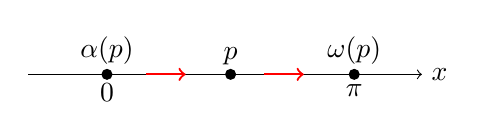
\begin{tikzpicture}
  \draw[->] (-1,0) -- (4,0) node[right] {$x$};
  \fill (0,0) circle (2pt) node[below] {$0$} node[above] {$\alpha(p)$};
  \fill (3.14,0) circle (2pt) node[below] {$\pi$} node[above] {$\omega(p)$};
  \fill (1.57,0) circle (2pt) node[above] {$p$};
  \draw[red,->,thick] (0.5,0) -- (1,0);
  \draw[red,->,thick] (2,0) -- (2.5,0);
\end{tikzpicture}

    \caption{Darstellung der Limesmengen aus Beispiel \ref{poinbendix:beispiel:1dlimesmengen}.}
    \label{poinbendix:fig:limesmenge}
\end{figure}
\end{beispiel}

\section{Der Satz von Poincaré-Bendixson} \label{poinbendix:section:poinbendix}

\begin{satz}[Poincaré-Bendixson]
\label{poinbendix:satz:poinbendix}
$\Phi_t(p) \in \Xi^r(\mathbb{S}^2)$ sei ein $r$-Fach differenzierbares, zweidimensionales dynamisches System mit Startpunkt $p \in \mathbb{S}^2$.
Dann gilt für das Omega-Limit Set $\omega(p)$ eine der folgenden Optionen:
\begin{enumerate}
\item $\omega(p)$ ist eine Nullstelle
\item $\omega(p)$ ist ein geschlossener Orbit
\item $\omega(p)$ ist ein geschlossener Orbit welcher Singularitäten verbindet
\end{enumerate}
\end{satz}

Dies gilt auf der Kugeloberfläche $\mathbb{S}^2$.\cite{poinbendix:melo}
Bis anhin haben wir aber mehrheitlich über planare Fälle gesprochen, weshalb der nächste Abschnitt darauf eingeht wieso wir hier die Kugeloberfläche nehmen.
In den darauffolgenden Abschnitten wird für dann jeden Fall jeweils ein Beispiel gezeigt.

\subsection{Kugeloberfläche und Ebene} \label{poinbendix:subsection:kugeloberflaeche}

Im Beispiel \ref{buch:koordinaten:diffmannig:beispiel:stereographisch} wird die stereographische Projektion eingeführt, welche ein planares Polarkoordinatensystem auf die Kugeloberfläche projiziert.
In Abbildung \ref{buch:koordinaten:diffmannig:fig:stereographisch} sieht man, dass dabei der Punkt auf dem Nordpol der Kugeloberfläche ins unendliche auf der Ebene abgebildet wird.
Somit ergibt sich für den Fall einer Nullstelle auf dem Nordpol eine divergierende Bahnkurve auf der Ebene.

Auch wenn die Formulierung auf der Kugeloberfläche etwas eleganter ist, gilt der Satz von Poincaré-Bendixson sowohl auf der Ebene $\mathbb{R}^2$ wie auch auf der Kugeloberfläche $\mathbb{S}^2$.
Allerdings gilt er nicht auf allen zweidimensionalen Abbildungen, so können zum Beispiel auf dem Torus Bahnkurven auftreten welche nicht wirklich periodisch sind, aber auch nicht auf eine Singularität fallen.\cite{poinbendix:wiki}


\subsection{Fall 1: $\omega(p)$ ist eine Nullstelle} \label{poinbendix:subsection:fall1}

Der erste Fall ist intuitiv am einfachsten zu verstehen.
Sobald auf einer Bahnkurve eine Nullstelle auftritt, bleibt die Kurve für alle Zeiten stehen.
Die eindimensionale Version von Fall 1  wurde bereits im Beispiel \ref{poinbendix:beispiel:1dlimesmengen} über die Limesmengen gezeigt.

\begin{beispiel} \label{poinbendix:beispiel:fall1}
Wir betrachten das folgende Differentialgleichungssystem:
\begin{align*}
    \dot{x} &= -x + y(1-x^2-y^2) \\
    \dot{y} &= -y - x(1-x^2-y^2).
\end{align*}
Nullstellen sind Punkte wo beide Ableitungen Null sind.
Zunächst substituieren wir den Klammerausdruck durch $a = (1-x^2-y^2)$ und setzen die Ableitung nach $x$ gleich Null
\begin{align*}
    -x + ya &= 0 \\
    ya &= x.
\end{align*}
Nun setzen wir dieses Resultat in die Ableitung nach $y$ und setzen es gleich Null
\begin{align*}
    -y - ya^2 &= 0 \\
    y(a^2+1) &= 0.
\end{align*}
Nach dieser Untersuchung sehen wir, dass es nur eine reelle Nullstelle $x=y=0$ geben kann, da $a^2 + 1$ im reellen nie Null werden kann.

Dieses Beispiel wurde gewählt da sehr schöne Bahnkurven entstehen.
Wie diese Bahnkurven aussehen können sieht man in Abbildung \ref{poinbendix:fig:fixed_point_omega_set}.
\end{beispiel}

Zu beachten gilt es, dass Satz von Poincaré-Bendixson nur eine Aussage zu möglichen Lösungen ab einem Startpunkt $p$ macht.
Dies würde unterschiedliche Fälle erlauben für ein einzelnes Differentialgleichungssystem.
Das obige Beispiel zeigt aber einen häufigen Fall, dass nämlich diverse Startpunkte $p$ dieselbe Nullstelle als Omega Limesmenge haben.

\begin{figure}
    \centering
    %% Creator: Matplotlib, PGF backend
%%
%% To include the figure in your LaTeX document, write
%%   \input{<filename>.pgf}
%%
%% Make sure the required packages are loaded in your preamble
%%   \usepackage{pgf}
%%
%% Also ensure that all the required font packages are loaded; for instance,
%% the lmodern package is sometimes necessary when using math font.
%%   \usepackage{lmodern}
%%
%% Figures using additional raster images can only be included by \input if
%% they are in the same directory as the main LaTeX file. For loading figures
%% from other directories you can use the `import` package
%%   \usepackage{import}
%%
%% and then include the figures with
%%   \import{<path to file>}{<filename>.pgf}
%%
%% Matplotlib used the following preamble
%%   \usepackage{bm}
%%   \usepackage{amsmath}
%%   \usepackage{xcolor}
%%   \usepackage{tgtermes}
%%   \makeatletter\@ifpackageloaded{underscore}{}{\usepackage[strings]{underscore}}\makeatother
%%
\begingroup%
\makeatletter%
\begin{pgfpicture}%
\pgfpathrectangle{\pgfpointorigin}{\pgfqpoint{4.500000in}{2.500000in}}%
\pgfusepath{use as bounding box, clip}%
\begin{pgfscope}%
\pgfsetbuttcap%
\pgfsetmiterjoin%
\definecolor{currentfill}{rgb}{1.000000,1.000000,1.000000}%
\pgfsetfillcolor{currentfill}%
\pgfsetlinewidth{0.000000pt}%
\definecolor{currentstroke}{rgb}{1.000000,1.000000,1.000000}%
\pgfsetstrokecolor{currentstroke}%
\pgfsetdash{}{0pt}%
\pgfpathmoveto{\pgfqpoint{0.000000in}{0.000000in}}%
\pgfpathlineto{\pgfqpoint{4.500000in}{0.000000in}}%
\pgfpathlineto{\pgfqpoint{4.500000in}{2.500000in}}%
\pgfpathlineto{\pgfqpoint{0.000000in}{2.500000in}}%
\pgfpathlineto{\pgfqpoint{0.000000in}{0.000000in}}%
\pgfpathclose%
\pgfusepath{fill}%
\end{pgfscope}%
\begin{pgfscope}%
\pgfsetbuttcap%
\pgfsetmiterjoin%
\definecolor{currentfill}{rgb}{1.000000,1.000000,1.000000}%
\pgfsetfillcolor{currentfill}%
\pgfsetlinewidth{0.000000pt}%
\definecolor{currentstroke}{rgb}{0.000000,0.000000,0.000000}%
\pgfsetstrokecolor{currentstroke}%
\pgfsetstrokeopacity{0.000000}%
\pgfsetdash{}{0pt}%
\pgfpathmoveto{\pgfqpoint{0.562500in}{0.275000in}}%
\pgfpathlineto{\pgfqpoint{4.050000in}{0.275000in}}%
\pgfpathlineto{\pgfqpoint{4.050000in}{2.200000in}}%
\pgfpathlineto{\pgfqpoint{0.562500in}{2.200000in}}%
\pgfpathlineto{\pgfqpoint{0.562500in}{0.275000in}}%
\pgfpathclose%
\pgfusepath{fill}%
\end{pgfscope}%
\begin{pgfscope}%
\pgfpathrectangle{\pgfqpoint{0.562500in}{0.275000in}}{\pgfqpoint{3.487500in}{1.925000in}}%
\pgfusepath{clip}%
\pgfsetrectcap%
\pgfsetroundjoin%
\pgfsetlinewidth{0.803000pt}%
\definecolor{currentstroke}{rgb}{0.690196,0.690196,0.690196}%
\pgfsetstrokecolor{currentstroke}%
\pgfsetdash{}{0pt}%
\pgfpathmoveto{\pgfqpoint{0.732791in}{0.275000in}}%
\pgfpathlineto{\pgfqpoint{0.732791in}{2.200000in}}%
\pgfusepath{stroke}%
\end{pgfscope}%
\begin{pgfscope}%
\pgfsetbuttcap%
\pgfsetroundjoin%
\definecolor{currentfill}{rgb}{0.000000,0.000000,0.000000}%
\pgfsetfillcolor{currentfill}%
\pgfsetlinewidth{0.803000pt}%
\definecolor{currentstroke}{rgb}{0.000000,0.000000,0.000000}%
\pgfsetstrokecolor{currentstroke}%
\pgfsetdash{}{0pt}%
\pgfsys@defobject{currentmarker}{\pgfqpoint{0.000000in}{-0.048611in}}{\pgfqpoint{0.000000in}{0.000000in}}{%
\pgfpathmoveto{\pgfqpoint{0.000000in}{0.000000in}}%
\pgfpathlineto{\pgfqpoint{0.000000in}{-0.048611in}}%
\pgfusepath{stroke,fill}%
}%
\begin{pgfscope}%
\pgfsys@transformshift{0.732791in}{0.275000in}%
\pgfsys@useobject{currentmarker}{}%
\end{pgfscope}%
\end{pgfscope}%
\begin{pgfscope}%
\definecolor{textcolor}{rgb}{0.000000,0.000000,0.000000}%
\pgfsetstrokecolor{textcolor}%
\pgfsetfillcolor{textcolor}%
\pgftext[x=0.732791in,y=0.177778in,,top]{\color{textcolor}\rmfamily\fontsize{10.000000}{12.000000}\selectfont \(\displaystyle {-1.0}\)}%
\end{pgfscope}%
\begin{pgfscope}%
\pgfpathrectangle{\pgfqpoint{0.562500in}{0.275000in}}{\pgfqpoint{3.487500in}{1.925000in}}%
\pgfusepath{clip}%
\pgfsetrectcap%
\pgfsetroundjoin%
\pgfsetlinewidth{0.803000pt}%
\definecolor{currentstroke}{rgb}{0.690196,0.690196,0.690196}%
\pgfsetstrokecolor{currentstroke}%
\pgfsetdash{}{0pt}%
\pgfpathmoveto{\pgfqpoint{1.522463in}{0.275000in}}%
\pgfpathlineto{\pgfqpoint{1.522463in}{2.200000in}}%
\pgfusepath{stroke}%
\end{pgfscope}%
\begin{pgfscope}%
\pgfsetbuttcap%
\pgfsetroundjoin%
\definecolor{currentfill}{rgb}{0.000000,0.000000,0.000000}%
\pgfsetfillcolor{currentfill}%
\pgfsetlinewidth{0.803000pt}%
\definecolor{currentstroke}{rgb}{0.000000,0.000000,0.000000}%
\pgfsetstrokecolor{currentstroke}%
\pgfsetdash{}{0pt}%
\pgfsys@defobject{currentmarker}{\pgfqpoint{0.000000in}{-0.048611in}}{\pgfqpoint{0.000000in}{0.000000in}}{%
\pgfpathmoveto{\pgfqpoint{0.000000in}{0.000000in}}%
\pgfpathlineto{\pgfqpoint{0.000000in}{-0.048611in}}%
\pgfusepath{stroke,fill}%
}%
\begin{pgfscope}%
\pgfsys@transformshift{1.522463in}{0.275000in}%
\pgfsys@useobject{currentmarker}{}%
\end{pgfscope}%
\end{pgfscope}%
\begin{pgfscope}%
\definecolor{textcolor}{rgb}{0.000000,0.000000,0.000000}%
\pgfsetstrokecolor{textcolor}%
\pgfsetfillcolor{textcolor}%
\pgftext[x=1.522463in,y=0.177778in,,top]{\color{textcolor}\rmfamily\fontsize{10.000000}{12.000000}\selectfont \(\displaystyle {-0.5}\)}%
\end{pgfscope}%
\begin{pgfscope}%
\pgfpathrectangle{\pgfqpoint{0.562500in}{0.275000in}}{\pgfqpoint{3.487500in}{1.925000in}}%
\pgfusepath{clip}%
\pgfsetrectcap%
\pgfsetroundjoin%
\pgfsetlinewidth{0.803000pt}%
\definecolor{currentstroke}{rgb}{0.690196,0.690196,0.690196}%
\pgfsetstrokecolor{currentstroke}%
\pgfsetdash{}{0pt}%
\pgfpathmoveto{\pgfqpoint{2.312134in}{0.275000in}}%
\pgfpathlineto{\pgfqpoint{2.312134in}{2.200000in}}%
\pgfusepath{stroke}%
\end{pgfscope}%
\begin{pgfscope}%
\pgfsetbuttcap%
\pgfsetroundjoin%
\definecolor{currentfill}{rgb}{0.000000,0.000000,0.000000}%
\pgfsetfillcolor{currentfill}%
\pgfsetlinewidth{0.803000pt}%
\definecolor{currentstroke}{rgb}{0.000000,0.000000,0.000000}%
\pgfsetstrokecolor{currentstroke}%
\pgfsetdash{}{0pt}%
\pgfsys@defobject{currentmarker}{\pgfqpoint{0.000000in}{-0.048611in}}{\pgfqpoint{0.000000in}{0.000000in}}{%
\pgfpathmoveto{\pgfqpoint{0.000000in}{0.000000in}}%
\pgfpathlineto{\pgfqpoint{0.000000in}{-0.048611in}}%
\pgfusepath{stroke,fill}%
}%
\begin{pgfscope}%
\pgfsys@transformshift{2.312134in}{0.275000in}%
\pgfsys@useobject{currentmarker}{}%
\end{pgfscope}%
\end{pgfscope}%
\begin{pgfscope}%
\definecolor{textcolor}{rgb}{0.000000,0.000000,0.000000}%
\pgfsetstrokecolor{textcolor}%
\pgfsetfillcolor{textcolor}%
\pgftext[x=2.312134in,y=0.177778in,,top]{\color{textcolor}\rmfamily\fontsize{10.000000}{12.000000}\selectfont \(\displaystyle {0.0}\)}%
\end{pgfscope}%
\begin{pgfscope}%
\pgfpathrectangle{\pgfqpoint{0.562500in}{0.275000in}}{\pgfqpoint{3.487500in}{1.925000in}}%
\pgfusepath{clip}%
\pgfsetrectcap%
\pgfsetroundjoin%
\pgfsetlinewidth{0.803000pt}%
\definecolor{currentstroke}{rgb}{0.690196,0.690196,0.690196}%
\pgfsetstrokecolor{currentstroke}%
\pgfsetdash{}{0pt}%
\pgfpathmoveto{\pgfqpoint{3.101806in}{0.275000in}}%
\pgfpathlineto{\pgfqpoint{3.101806in}{2.200000in}}%
\pgfusepath{stroke}%
\end{pgfscope}%
\begin{pgfscope}%
\pgfsetbuttcap%
\pgfsetroundjoin%
\definecolor{currentfill}{rgb}{0.000000,0.000000,0.000000}%
\pgfsetfillcolor{currentfill}%
\pgfsetlinewidth{0.803000pt}%
\definecolor{currentstroke}{rgb}{0.000000,0.000000,0.000000}%
\pgfsetstrokecolor{currentstroke}%
\pgfsetdash{}{0pt}%
\pgfsys@defobject{currentmarker}{\pgfqpoint{0.000000in}{-0.048611in}}{\pgfqpoint{0.000000in}{0.000000in}}{%
\pgfpathmoveto{\pgfqpoint{0.000000in}{0.000000in}}%
\pgfpathlineto{\pgfqpoint{0.000000in}{-0.048611in}}%
\pgfusepath{stroke,fill}%
}%
\begin{pgfscope}%
\pgfsys@transformshift{3.101806in}{0.275000in}%
\pgfsys@useobject{currentmarker}{}%
\end{pgfscope}%
\end{pgfscope}%
\begin{pgfscope}%
\definecolor{textcolor}{rgb}{0.000000,0.000000,0.000000}%
\pgfsetstrokecolor{textcolor}%
\pgfsetfillcolor{textcolor}%
\pgftext[x=3.101806in,y=0.177778in,,top]{\color{textcolor}\rmfamily\fontsize{10.000000}{12.000000}\selectfont \(\displaystyle {0.5}\)}%
\end{pgfscope}%
\begin{pgfscope}%
\pgfpathrectangle{\pgfqpoint{0.562500in}{0.275000in}}{\pgfqpoint{3.487500in}{1.925000in}}%
\pgfusepath{clip}%
\pgfsetrectcap%
\pgfsetroundjoin%
\pgfsetlinewidth{0.803000pt}%
\definecolor{currentstroke}{rgb}{0.690196,0.690196,0.690196}%
\pgfsetstrokecolor{currentstroke}%
\pgfsetdash{}{0pt}%
\pgfpathmoveto{\pgfqpoint{3.891477in}{0.275000in}}%
\pgfpathlineto{\pgfqpoint{3.891477in}{2.200000in}}%
\pgfusepath{stroke}%
\end{pgfscope}%
\begin{pgfscope}%
\pgfsetbuttcap%
\pgfsetroundjoin%
\definecolor{currentfill}{rgb}{0.000000,0.000000,0.000000}%
\pgfsetfillcolor{currentfill}%
\pgfsetlinewidth{0.803000pt}%
\definecolor{currentstroke}{rgb}{0.000000,0.000000,0.000000}%
\pgfsetstrokecolor{currentstroke}%
\pgfsetdash{}{0pt}%
\pgfsys@defobject{currentmarker}{\pgfqpoint{0.000000in}{-0.048611in}}{\pgfqpoint{0.000000in}{0.000000in}}{%
\pgfpathmoveto{\pgfqpoint{0.000000in}{0.000000in}}%
\pgfpathlineto{\pgfqpoint{0.000000in}{-0.048611in}}%
\pgfusepath{stroke,fill}%
}%
\begin{pgfscope}%
\pgfsys@transformshift{3.891477in}{0.275000in}%
\pgfsys@useobject{currentmarker}{}%
\end{pgfscope}%
\end{pgfscope}%
\begin{pgfscope}%
\definecolor{textcolor}{rgb}{0.000000,0.000000,0.000000}%
\pgfsetstrokecolor{textcolor}%
\pgfsetfillcolor{textcolor}%
\pgftext[x=3.891477in,y=0.177778in,,top]{\color{textcolor}\rmfamily\fontsize{10.000000}{12.000000}\selectfont \(\displaystyle {1.0}\)}%
\end{pgfscope}%
\begin{pgfscope}%
\pgfpathrectangle{\pgfqpoint{0.562500in}{0.275000in}}{\pgfqpoint{3.487500in}{1.925000in}}%
\pgfusepath{clip}%
\pgfsetrectcap%
\pgfsetroundjoin%
\pgfsetlinewidth{0.803000pt}%
\definecolor{currentstroke}{rgb}{0.690196,0.690196,0.690196}%
\pgfsetstrokecolor{currentstroke}%
\pgfsetdash{}{0pt}%
\pgfpathmoveto{\pgfqpoint{0.562500in}{0.362500in}}%
\pgfpathlineto{\pgfqpoint{4.050000in}{0.362500in}}%
\pgfusepath{stroke}%
\end{pgfscope}%
\begin{pgfscope}%
\pgfsetbuttcap%
\pgfsetroundjoin%
\definecolor{currentfill}{rgb}{0.000000,0.000000,0.000000}%
\pgfsetfillcolor{currentfill}%
\pgfsetlinewidth{0.803000pt}%
\definecolor{currentstroke}{rgb}{0.000000,0.000000,0.000000}%
\pgfsetstrokecolor{currentstroke}%
\pgfsetdash{}{0pt}%
\pgfsys@defobject{currentmarker}{\pgfqpoint{-0.048611in}{0.000000in}}{\pgfqpoint{-0.000000in}{0.000000in}}{%
\pgfpathmoveto{\pgfqpoint{-0.000000in}{0.000000in}}%
\pgfpathlineto{\pgfqpoint{-0.048611in}{0.000000in}}%
\pgfusepath{stroke,fill}%
}%
\begin{pgfscope}%
\pgfsys@transformshift{0.562500in}{0.362500in}%
\pgfsys@useobject{currentmarker}{}%
\end{pgfscope}%
\end{pgfscope}%
\begin{pgfscope}%
\definecolor{textcolor}{rgb}{0.000000,0.000000,0.000000}%
\pgfsetstrokecolor{textcolor}%
\pgfsetfillcolor{textcolor}%
\pgftext[x=0.287808in, y=0.315799in, left, base]{\color{textcolor}\rmfamily\fontsize{10.000000}{12.000000}\selectfont \(\displaystyle {-1}\)}%
\end{pgfscope}%
\begin{pgfscope}%
\pgfpathrectangle{\pgfqpoint{0.562500in}{0.275000in}}{\pgfqpoint{3.487500in}{1.925000in}}%
\pgfusepath{clip}%
\pgfsetrectcap%
\pgfsetroundjoin%
\pgfsetlinewidth{0.803000pt}%
\definecolor{currentstroke}{rgb}{0.690196,0.690196,0.690196}%
\pgfsetstrokecolor{currentstroke}%
\pgfsetdash{}{0pt}%
\pgfpathmoveto{\pgfqpoint{0.562500in}{0.943734in}}%
\pgfpathlineto{\pgfqpoint{4.050000in}{0.943734in}}%
\pgfusepath{stroke}%
\end{pgfscope}%
\begin{pgfscope}%
\pgfsetbuttcap%
\pgfsetroundjoin%
\definecolor{currentfill}{rgb}{0.000000,0.000000,0.000000}%
\pgfsetfillcolor{currentfill}%
\pgfsetlinewidth{0.803000pt}%
\definecolor{currentstroke}{rgb}{0.000000,0.000000,0.000000}%
\pgfsetstrokecolor{currentstroke}%
\pgfsetdash{}{0pt}%
\pgfsys@defobject{currentmarker}{\pgfqpoint{-0.048611in}{0.000000in}}{\pgfqpoint{-0.000000in}{0.000000in}}{%
\pgfpathmoveto{\pgfqpoint{-0.000000in}{0.000000in}}%
\pgfpathlineto{\pgfqpoint{-0.048611in}{0.000000in}}%
\pgfusepath{stroke,fill}%
}%
\begin{pgfscope}%
\pgfsys@transformshift{0.562500in}{0.943734in}%
\pgfsys@useobject{currentmarker}{}%
\end{pgfscope}%
\end{pgfscope}%
\begin{pgfscope}%
\definecolor{textcolor}{rgb}{0.000000,0.000000,0.000000}%
\pgfsetstrokecolor{textcolor}%
\pgfsetfillcolor{textcolor}%
\pgftext[x=0.395833in, y=0.897032in, left, base]{\color{textcolor}\rmfamily\fontsize{10.000000}{12.000000}\selectfont \(\displaystyle {0}\)}%
\end{pgfscope}%
\begin{pgfscope}%
\pgfpathrectangle{\pgfqpoint{0.562500in}{0.275000in}}{\pgfqpoint{3.487500in}{1.925000in}}%
\pgfusepath{clip}%
\pgfsetrectcap%
\pgfsetroundjoin%
\pgfsetlinewidth{0.803000pt}%
\definecolor{currentstroke}{rgb}{0.690196,0.690196,0.690196}%
\pgfsetstrokecolor{currentstroke}%
\pgfsetdash{}{0pt}%
\pgfpathmoveto{\pgfqpoint{0.562500in}{1.524967in}}%
\pgfpathlineto{\pgfqpoint{4.050000in}{1.524967in}}%
\pgfusepath{stroke}%
\end{pgfscope}%
\begin{pgfscope}%
\pgfsetbuttcap%
\pgfsetroundjoin%
\definecolor{currentfill}{rgb}{0.000000,0.000000,0.000000}%
\pgfsetfillcolor{currentfill}%
\pgfsetlinewidth{0.803000pt}%
\definecolor{currentstroke}{rgb}{0.000000,0.000000,0.000000}%
\pgfsetstrokecolor{currentstroke}%
\pgfsetdash{}{0pt}%
\pgfsys@defobject{currentmarker}{\pgfqpoint{-0.048611in}{0.000000in}}{\pgfqpoint{-0.000000in}{0.000000in}}{%
\pgfpathmoveto{\pgfqpoint{-0.000000in}{0.000000in}}%
\pgfpathlineto{\pgfqpoint{-0.048611in}{0.000000in}}%
\pgfusepath{stroke,fill}%
}%
\begin{pgfscope}%
\pgfsys@transformshift{0.562500in}{1.524967in}%
\pgfsys@useobject{currentmarker}{}%
\end{pgfscope}%
\end{pgfscope}%
\begin{pgfscope}%
\definecolor{textcolor}{rgb}{0.000000,0.000000,0.000000}%
\pgfsetstrokecolor{textcolor}%
\pgfsetfillcolor{textcolor}%
\pgftext[x=0.395833in, y=1.478266in, left, base]{\color{textcolor}\rmfamily\fontsize{10.000000}{12.000000}\selectfont \(\displaystyle {1}\)}%
\end{pgfscope}%
\begin{pgfscope}%
\pgfpathrectangle{\pgfqpoint{0.562500in}{0.275000in}}{\pgfqpoint{3.487500in}{1.925000in}}%
\pgfusepath{clip}%
\pgfsetrectcap%
\pgfsetroundjoin%
\pgfsetlinewidth{0.803000pt}%
\definecolor{currentstroke}{rgb}{0.690196,0.690196,0.690196}%
\pgfsetstrokecolor{currentstroke}%
\pgfsetdash{}{0pt}%
\pgfpathmoveto{\pgfqpoint{0.562500in}{2.106201in}}%
\pgfpathlineto{\pgfqpoint{4.050000in}{2.106201in}}%
\pgfusepath{stroke}%
\end{pgfscope}%
\begin{pgfscope}%
\pgfsetbuttcap%
\pgfsetroundjoin%
\definecolor{currentfill}{rgb}{0.000000,0.000000,0.000000}%
\pgfsetfillcolor{currentfill}%
\pgfsetlinewidth{0.803000pt}%
\definecolor{currentstroke}{rgb}{0.000000,0.000000,0.000000}%
\pgfsetstrokecolor{currentstroke}%
\pgfsetdash{}{0pt}%
\pgfsys@defobject{currentmarker}{\pgfqpoint{-0.048611in}{0.000000in}}{\pgfqpoint{-0.000000in}{0.000000in}}{%
\pgfpathmoveto{\pgfqpoint{-0.000000in}{0.000000in}}%
\pgfpathlineto{\pgfqpoint{-0.048611in}{0.000000in}}%
\pgfusepath{stroke,fill}%
}%
\begin{pgfscope}%
\pgfsys@transformshift{0.562500in}{2.106201in}%
\pgfsys@useobject{currentmarker}{}%
\end{pgfscope}%
\end{pgfscope}%
\begin{pgfscope}%
\definecolor{textcolor}{rgb}{0.000000,0.000000,0.000000}%
\pgfsetstrokecolor{textcolor}%
\pgfsetfillcolor{textcolor}%
\pgftext[x=0.395833in, y=2.059500in, left, base]{\color{textcolor}\rmfamily\fontsize{10.000000}{12.000000}\selectfont \(\displaystyle {2}\)}%
\end{pgfscope}%
\begin{pgfscope}%
\pgfpathrectangle{\pgfqpoint{0.562500in}{0.275000in}}{\pgfqpoint{3.487500in}{1.925000in}}%
\pgfusepath{clip}%
\pgfsetbuttcap%
\pgfsetroundjoin%
\definecolor{currentfill}{rgb}{0.121569,0.466667,0.705882}%
\pgfsetfillcolor{currentfill}%
\pgfsetlinewidth{1.003750pt}%
\definecolor{currentstroke}{rgb}{0.121569,0.466667,0.705882}%
\pgfsetstrokecolor{currentstroke}%
\pgfsetdash{}{0pt}%
\pgfsys@defobject{currentmarker}{\pgfqpoint{-0.020833in}{-0.020833in}}{\pgfqpoint{0.020833in}{0.020833in}}{%
\pgfpathmoveto{\pgfqpoint{0.000000in}{-0.020833in}}%
\pgfpathcurveto{\pgfqpoint{0.005525in}{-0.020833in}}{\pgfqpoint{0.010825in}{-0.018638in}}{\pgfqpoint{0.014731in}{-0.014731in}}%
\pgfpathcurveto{\pgfqpoint{0.018638in}{-0.010825in}}{\pgfqpoint{0.020833in}{-0.005525in}}{\pgfqpoint{0.020833in}{0.000000in}}%
\pgfpathcurveto{\pgfqpoint{0.020833in}{0.005525in}}{\pgfqpoint{0.018638in}{0.010825in}}{\pgfqpoint{0.014731in}{0.014731in}}%
\pgfpathcurveto{\pgfqpoint{0.010825in}{0.018638in}}{\pgfqpoint{0.005525in}{0.020833in}}{\pgfqpoint{0.000000in}{0.020833in}}%
\pgfpathcurveto{\pgfqpoint{-0.005525in}{0.020833in}}{\pgfqpoint{-0.010825in}{0.018638in}}{\pgfqpoint{-0.014731in}{0.014731in}}%
\pgfpathcurveto{\pgfqpoint{-0.018638in}{0.010825in}}{\pgfqpoint{-0.020833in}{0.005525in}}{\pgfqpoint{-0.020833in}{0.000000in}}%
\pgfpathcurveto{\pgfqpoint{-0.020833in}{-0.005525in}}{\pgfqpoint{-0.018638in}{-0.010825in}}{\pgfqpoint{-0.014731in}{-0.014731in}}%
\pgfpathcurveto{\pgfqpoint{-0.010825in}{-0.018638in}}{\pgfqpoint{-0.005525in}{-0.020833in}}{\pgfqpoint{0.000000in}{-0.020833in}}%
\pgfpathlineto{\pgfqpoint{0.000000in}{-0.020833in}}%
\pgfpathclose%
\pgfusepath{stroke,fill}%
}%
\begin{pgfscope}%
\pgfsys@transformshift{2.312134in}{0.943734in}%
\pgfsys@useobject{currentmarker}{}%
\end{pgfscope}%
\begin{pgfscope}%
\pgfsys@transformshift{2.312134in}{0.943734in}%
\pgfsys@useobject{currentmarker}{}%
\end{pgfscope}%
\begin{pgfscope}%
\pgfsys@transformshift{2.312134in}{0.943734in}%
\pgfsys@useobject{currentmarker}{}%
\end{pgfscope}%
\begin{pgfscope}%
\pgfsys@transformshift{2.312134in}{0.943734in}%
\pgfsys@useobject{currentmarker}{}%
\end{pgfscope}%
\begin{pgfscope}%
\pgfsys@transformshift{2.312134in}{0.943734in}%
\pgfsys@useobject{currentmarker}{}%
\end{pgfscope}%
\begin{pgfscope}%
\pgfsys@transformshift{2.312134in}{0.943734in}%
\pgfsys@useobject{currentmarker}{}%
\end{pgfscope}%
\begin{pgfscope}%
\pgfsys@transformshift{2.312134in}{0.943734in}%
\pgfsys@useobject{currentmarker}{}%
\end{pgfscope}%
\begin{pgfscope}%
\pgfsys@transformshift{2.312134in}{0.943734in}%
\pgfsys@useobject{currentmarker}{}%
\end{pgfscope}%
\begin{pgfscope}%
\pgfsys@transformshift{2.312134in}{0.943734in}%
\pgfsys@useobject{currentmarker}{}%
\end{pgfscope}%
\begin{pgfscope}%
\pgfsys@transformshift{2.312134in}{0.943734in}%
\pgfsys@useobject{currentmarker}{}%
\end{pgfscope}%
\begin{pgfscope}%
\pgfsys@transformshift{2.312134in}{0.943734in}%
\pgfsys@useobject{currentmarker}{}%
\end{pgfscope}%
\begin{pgfscope}%
\pgfsys@transformshift{2.312134in}{0.943734in}%
\pgfsys@useobject{currentmarker}{}%
\end{pgfscope}%
\begin{pgfscope}%
\pgfsys@transformshift{2.312134in}{0.943734in}%
\pgfsys@useobject{currentmarker}{}%
\end{pgfscope}%
\begin{pgfscope}%
\pgfsys@transformshift{2.312134in}{0.943734in}%
\pgfsys@useobject{currentmarker}{}%
\end{pgfscope}%
\begin{pgfscope}%
\pgfsys@transformshift{2.312134in}{0.943734in}%
\pgfsys@useobject{currentmarker}{}%
\end{pgfscope}%
\begin{pgfscope}%
\pgfsys@transformshift{2.312134in}{0.943734in}%
\pgfsys@useobject{currentmarker}{}%
\end{pgfscope}%
\begin{pgfscope}%
\pgfsys@transformshift{2.312134in}{0.943734in}%
\pgfsys@useobject{currentmarker}{}%
\end{pgfscope}%
\begin{pgfscope}%
\pgfsys@transformshift{2.312134in}{0.943734in}%
\pgfsys@useobject{currentmarker}{}%
\end{pgfscope}%
\begin{pgfscope}%
\pgfsys@transformshift{2.312134in}{0.943734in}%
\pgfsys@useobject{currentmarker}{}%
\end{pgfscope}%
\begin{pgfscope}%
\pgfsys@transformshift{2.312134in}{0.943734in}%
\pgfsys@useobject{currentmarker}{}%
\end{pgfscope}%
\begin{pgfscope}%
\pgfsys@transformshift{2.312134in}{0.943734in}%
\pgfsys@useobject{currentmarker}{}%
\end{pgfscope}%
\begin{pgfscope}%
\pgfsys@transformshift{2.312134in}{0.943734in}%
\pgfsys@useobject{currentmarker}{}%
\end{pgfscope}%
\begin{pgfscope}%
\pgfsys@transformshift{2.312134in}{0.943734in}%
\pgfsys@useobject{currentmarker}{}%
\end{pgfscope}%
\begin{pgfscope}%
\pgfsys@transformshift{2.312134in}{0.943734in}%
\pgfsys@useobject{currentmarker}{}%
\end{pgfscope}%
\begin{pgfscope}%
\pgfsys@transformshift{2.312134in}{0.943734in}%
\pgfsys@useobject{currentmarker}{}%
\end{pgfscope}%
\begin{pgfscope}%
\pgfsys@transformshift{2.312134in}{0.943734in}%
\pgfsys@useobject{currentmarker}{}%
\end{pgfscope}%
\begin{pgfscope}%
\pgfsys@transformshift{2.312134in}{0.943734in}%
\pgfsys@useobject{currentmarker}{}%
\end{pgfscope}%
\begin{pgfscope}%
\pgfsys@transformshift{2.312134in}{0.943734in}%
\pgfsys@useobject{currentmarker}{}%
\end{pgfscope}%
\begin{pgfscope}%
\pgfsys@transformshift{2.312134in}{0.943734in}%
\pgfsys@useobject{currentmarker}{}%
\end{pgfscope}%
\begin{pgfscope}%
\pgfsys@transformshift{2.312134in}{0.943734in}%
\pgfsys@useobject{currentmarker}{}%
\end{pgfscope}%
\begin{pgfscope}%
\pgfsys@transformshift{2.312134in}{0.943734in}%
\pgfsys@useobject{currentmarker}{}%
\end{pgfscope}%
\begin{pgfscope}%
\pgfsys@transformshift{2.312134in}{0.943734in}%
\pgfsys@useobject{currentmarker}{}%
\end{pgfscope}%
\begin{pgfscope}%
\pgfsys@transformshift{2.312134in}{0.943734in}%
\pgfsys@useobject{currentmarker}{}%
\end{pgfscope}%
\begin{pgfscope}%
\pgfsys@transformshift{2.312134in}{0.943734in}%
\pgfsys@useobject{currentmarker}{}%
\end{pgfscope}%
\begin{pgfscope}%
\pgfsys@transformshift{2.312134in}{0.943734in}%
\pgfsys@useobject{currentmarker}{}%
\end{pgfscope}%
\begin{pgfscope}%
\pgfsys@transformshift{2.312134in}{0.943734in}%
\pgfsys@useobject{currentmarker}{}%
\end{pgfscope}%
\begin{pgfscope}%
\pgfsys@transformshift{2.312134in}{0.943734in}%
\pgfsys@useobject{currentmarker}{}%
\end{pgfscope}%
\begin{pgfscope}%
\pgfsys@transformshift{2.312134in}{0.943734in}%
\pgfsys@useobject{currentmarker}{}%
\end{pgfscope}%
\begin{pgfscope}%
\pgfsys@transformshift{2.312134in}{0.943734in}%
\pgfsys@useobject{currentmarker}{}%
\end{pgfscope}%
\begin{pgfscope}%
\pgfsys@transformshift{2.312134in}{0.943734in}%
\pgfsys@useobject{currentmarker}{}%
\end{pgfscope}%
\begin{pgfscope}%
\pgfsys@transformshift{2.312134in}{0.943734in}%
\pgfsys@useobject{currentmarker}{}%
\end{pgfscope}%
\begin{pgfscope}%
\pgfsys@transformshift{2.312134in}{0.943734in}%
\pgfsys@useobject{currentmarker}{}%
\end{pgfscope}%
\begin{pgfscope}%
\pgfsys@transformshift{2.312134in}{0.943734in}%
\pgfsys@useobject{currentmarker}{}%
\end{pgfscope}%
\begin{pgfscope}%
\pgfsys@transformshift{2.312134in}{0.943734in}%
\pgfsys@useobject{currentmarker}{}%
\end{pgfscope}%
\begin{pgfscope}%
\pgfsys@transformshift{2.312134in}{0.943734in}%
\pgfsys@useobject{currentmarker}{}%
\end{pgfscope}%
\begin{pgfscope}%
\pgfsys@transformshift{2.312134in}{0.943734in}%
\pgfsys@useobject{currentmarker}{}%
\end{pgfscope}%
\begin{pgfscope}%
\pgfsys@transformshift{2.312134in}{0.943734in}%
\pgfsys@useobject{currentmarker}{}%
\end{pgfscope}%
\begin{pgfscope}%
\pgfsys@transformshift{2.312134in}{0.943734in}%
\pgfsys@useobject{currentmarker}{}%
\end{pgfscope}%
\begin{pgfscope}%
\pgfsys@transformshift{2.312134in}{0.943734in}%
\pgfsys@useobject{currentmarker}{}%
\end{pgfscope}%
\begin{pgfscope}%
\pgfsys@transformshift{2.312134in}{0.943734in}%
\pgfsys@useobject{currentmarker}{}%
\end{pgfscope}%
\begin{pgfscope}%
\pgfsys@transformshift{2.312134in}{0.943734in}%
\pgfsys@useobject{currentmarker}{}%
\end{pgfscope}%
\begin{pgfscope}%
\pgfsys@transformshift{2.312134in}{0.943734in}%
\pgfsys@useobject{currentmarker}{}%
\end{pgfscope}%
\begin{pgfscope}%
\pgfsys@transformshift{2.312134in}{0.943734in}%
\pgfsys@useobject{currentmarker}{}%
\end{pgfscope}%
\begin{pgfscope}%
\pgfsys@transformshift{2.312134in}{0.943734in}%
\pgfsys@useobject{currentmarker}{}%
\end{pgfscope}%
\begin{pgfscope}%
\pgfsys@transformshift{2.312134in}{0.943734in}%
\pgfsys@useobject{currentmarker}{}%
\end{pgfscope}%
\begin{pgfscope}%
\pgfsys@transformshift{2.312134in}{0.943734in}%
\pgfsys@useobject{currentmarker}{}%
\end{pgfscope}%
\begin{pgfscope}%
\pgfsys@transformshift{2.312134in}{0.943734in}%
\pgfsys@useobject{currentmarker}{}%
\end{pgfscope}%
\begin{pgfscope}%
\pgfsys@transformshift{2.312134in}{0.943734in}%
\pgfsys@useobject{currentmarker}{}%
\end{pgfscope}%
\begin{pgfscope}%
\pgfsys@transformshift{2.312134in}{0.943734in}%
\pgfsys@useobject{currentmarker}{}%
\end{pgfscope}%
\begin{pgfscope}%
\pgfsys@transformshift{2.312134in}{0.943734in}%
\pgfsys@useobject{currentmarker}{}%
\end{pgfscope}%
\begin{pgfscope}%
\pgfsys@transformshift{2.312134in}{0.943734in}%
\pgfsys@useobject{currentmarker}{}%
\end{pgfscope}%
\begin{pgfscope}%
\pgfsys@transformshift{2.312134in}{0.943734in}%
\pgfsys@useobject{currentmarker}{}%
\end{pgfscope}%
\begin{pgfscope}%
\pgfsys@transformshift{2.312134in}{0.943734in}%
\pgfsys@useobject{currentmarker}{}%
\end{pgfscope}%
\begin{pgfscope}%
\pgfsys@transformshift{2.312134in}{0.943734in}%
\pgfsys@useobject{currentmarker}{}%
\end{pgfscope}%
\begin{pgfscope}%
\pgfsys@transformshift{2.312134in}{0.943734in}%
\pgfsys@useobject{currentmarker}{}%
\end{pgfscope}%
\begin{pgfscope}%
\pgfsys@transformshift{2.312134in}{0.943734in}%
\pgfsys@useobject{currentmarker}{}%
\end{pgfscope}%
\begin{pgfscope}%
\pgfsys@transformshift{2.312134in}{0.943734in}%
\pgfsys@useobject{currentmarker}{}%
\end{pgfscope}%
\begin{pgfscope}%
\pgfsys@transformshift{2.312134in}{0.943734in}%
\pgfsys@useobject{currentmarker}{}%
\end{pgfscope}%
\begin{pgfscope}%
\pgfsys@transformshift{2.312134in}{0.943734in}%
\pgfsys@useobject{currentmarker}{}%
\end{pgfscope}%
\begin{pgfscope}%
\pgfsys@transformshift{2.312134in}{0.943734in}%
\pgfsys@useobject{currentmarker}{}%
\end{pgfscope}%
\begin{pgfscope}%
\pgfsys@transformshift{2.312134in}{0.943734in}%
\pgfsys@useobject{currentmarker}{}%
\end{pgfscope}%
\begin{pgfscope}%
\pgfsys@transformshift{2.312134in}{0.943734in}%
\pgfsys@useobject{currentmarker}{}%
\end{pgfscope}%
\begin{pgfscope}%
\pgfsys@transformshift{2.312134in}{0.943734in}%
\pgfsys@useobject{currentmarker}{}%
\end{pgfscope}%
\begin{pgfscope}%
\pgfsys@transformshift{2.312134in}{0.943734in}%
\pgfsys@useobject{currentmarker}{}%
\end{pgfscope}%
\begin{pgfscope}%
\pgfsys@transformshift{2.312134in}{0.943734in}%
\pgfsys@useobject{currentmarker}{}%
\end{pgfscope}%
\begin{pgfscope}%
\pgfsys@transformshift{2.312134in}{0.943734in}%
\pgfsys@useobject{currentmarker}{}%
\end{pgfscope}%
\begin{pgfscope}%
\pgfsys@transformshift{2.312134in}{0.943734in}%
\pgfsys@useobject{currentmarker}{}%
\end{pgfscope}%
\begin{pgfscope}%
\pgfsys@transformshift{2.312134in}{0.943734in}%
\pgfsys@useobject{currentmarker}{}%
\end{pgfscope}%
\begin{pgfscope}%
\pgfsys@transformshift{2.312134in}{0.943734in}%
\pgfsys@useobject{currentmarker}{}%
\end{pgfscope}%
\begin{pgfscope}%
\pgfsys@transformshift{2.312134in}{0.943734in}%
\pgfsys@useobject{currentmarker}{}%
\end{pgfscope}%
\begin{pgfscope}%
\pgfsys@transformshift{2.312134in}{0.943734in}%
\pgfsys@useobject{currentmarker}{}%
\end{pgfscope}%
\begin{pgfscope}%
\pgfsys@transformshift{2.312134in}{0.943734in}%
\pgfsys@useobject{currentmarker}{}%
\end{pgfscope}%
\begin{pgfscope}%
\pgfsys@transformshift{2.312134in}{0.943734in}%
\pgfsys@useobject{currentmarker}{}%
\end{pgfscope}%
\begin{pgfscope}%
\pgfsys@transformshift{2.312134in}{0.943734in}%
\pgfsys@useobject{currentmarker}{}%
\end{pgfscope}%
\begin{pgfscope}%
\pgfsys@transformshift{2.312134in}{0.943734in}%
\pgfsys@useobject{currentmarker}{}%
\end{pgfscope}%
\begin{pgfscope}%
\pgfsys@transformshift{2.312134in}{0.943734in}%
\pgfsys@useobject{currentmarker}{}%
\end{pgfscope}%
\begin{pgfscope}%
\pgfsys@transformshift{2.312134in}{0.943734in}%
\pgfsys@useobject{currentmarker}{}%
\end{pgfscope}%
\begin{pgfscope}%
\pgfsys@transformshift{2.312134in}{0.943734in}%
\pgfsys@useobject{currentmarker}{}%
\end{pgfscope}%
\begin{pgfscope}%
\pgfsys@transformshift{2.312134in}{0.943734in}%
\pgfsys@useobject{currentmarker}{}%
\end{pgfscope}%
\begin{pgfscope}%
\pgfsys@transformshift{2.312134in}{0.943734in}%
\pgfsys@useobject{currentmarker}{}%
\end{pgfscope}%
\begin{pgfscope}%
\pgfsys@transformshift{2.312134in}{0.943734in}%
\pgfsys@useobject{currentmarker}{}%
\end{pgfscope}%
\begin{pgfscope}%
\pgfsys@transformshift{2.312134in}{0.943734in}%
\pgfsys@useobject{currentmarker}{}%
\end{pgfscope}%
\begin{pgfscope}%
\pgfsys@transformshift{2.312134in}{0.943734in}%
\pgfsys@useobject{currentmarker}{}%
\end{pgfscope}%
\begin{pgfscope}%
\pgfsys@transformshift{2.312134in}{0.943734in}%
\pgfsys@useobject{currentmarker}{}%
\end{pgfscope}%
\begin{pgfscope}%
\pgfsys@transformshift{2.312134in}{0.943734in}%
\pgfsys@useobject{currentmarker}{}%
\end{pgfscope}%
\begin{pgfscope}%
\pgfsys@transformshift{2.312134in}{0.943734in}%
\pgfsys@useobject{currentmarker}{}%
\end{pgfscope}%
\begin{pgfscope}%
\pgfsys@transformshift{2.312134in}{0.943734in}%
\pgfsys@useobject{currentmarker}{}%
\end{pgfscope}%
\begin{pgfscope}%
\pgfsys@transformshift{2.312134in}{0.943734in}%
\pgfsys@useobject{currentmarker}{}%
\end{pgfscope}%
\begin{pgfscope}%
\pgfsys@transformshift{2.312134in}{0.943734in}%
\pgfsys@useobject{currentmarker}{}%
\end{pgfscope}%
\begin{pgfscope}%
\pgfsys@transformshift{2.312134in}{0.943734in}%
\pgfsys@useobject{currentmarker}{}%
\end{pgfscope}%
\begin{pgfscope}%
\pgfsys@transformshift{2.312134in}{0.943734in}%
\pgfsys@useobject{currentmarker}{}%
\end{pgfscope}%
\begin{pgfscope}%
\pgfsys@transformshift{2.312134in}{0.943734in}%
\pgfsys@useobject{currentmarker}{}%
\end{pgfscope}%
\begin{pgfscope}%
\pgfsys@transformshift{2.312134in}{0.943734in}%
\pgfsys@useobject{currentmarker}{}%
\end{pgfscope}%
\begin{pgfscope}%
\pgfsys@transformshift{2.312134in}{0.943734in}%
\pgfsys@useobject{currentmarker}{}%
\end{pgfscope}%
\begin{pgfscope}%
\pgfsys@transformshift{2.312134in}{0.943734in}%
\pgfsys@useobject{currentmarker}{}%
\end{pgfscope}%
\begin{pgfscope}%
\pgfsys@transformshift{2.312134in}{0.943734in}%
\pgfsys@useobject{currentmarker}{}%
\end{pgfscope}%
\begin{pgfscope}%
\pgfsys@transformshift{2.312134in}{0.943734in}%
\pgfsys@useobject{currentmarker}{}%
\end{pgfscope}%
\begin{pgfscope}%
\pgfsys@transformshift{2.312134in}{0.943734in}%
\pgfsys@useobject{currentmarker}{}%
\end{pgfscope}%
\begin{pgfscope}%
\pgfsys@transformshift{2.312134in}{0.943734in}%
\pgfsys@useobject{currentmarker}{}%
\end{pgfscope}%
\begin{pgfscope}%
\pgfsys@transformshift{2.312134in}{0.943734in}%
\pgfsys@useobject{currentmarker}{}%
\end{pgfscope}%
\begin{pgfscope}%
\pgfsys@transformshift{2.312134in}{0.943734in}%
\pgfsys@useobject{currentmarker}{}%
\end{pgfscope}%
\begin{pgfscope}%
\pgfsys@transformshift{2.312134in}{0.943734in}%
\pgfsys@useobject{currentmarker}{}%
\end{pgfscope}%
\begin{pgfscope}%
\pgfsys@transformshift{2.312134in}{0.943734in}%
\pgfsys@useobject{currentmarker}{}%
\end{pgfscope}%
\begin{pgfscope}%
\pgfsys@transformshift{2.312134in}{0.943734in}%
\pgfsys@useobject{currentmarker}{}%
\end{pgfscope}%
\begin{pgfscope}%
\pgfsys@transformshift{2.312134in}{0.943734in}%
\pgfsys@useobject{currentmarker}{}%
\end{pgfscope}%
\begin{pgfscope}%
\pgfsys@transformshift{2.312134in}{0.943734in}%
\pgfsys@useobject{currentmarker}{}%
\end{pgfscope}%
\begin{pgfscope}%
\pgfsys@transformshift{2.312134in}{0.943734in}%
\pgfsys@useobject{currentmarker}{}%
\end{pgfscope}%
\begin{pgfscope}%
\pgfsys@transformshift{2.312134in}{0.943734in}%
\pgfsys@useobject{currentmarker}{}%
\end{pgfscope}%
\begin{pgfscope}%
\pgfsys@transformshift{2.312134in}{0.943734in}%
\pgfsys@useobject{currentmarker}{}%
\end{pgfscope}%
\begin{pgfscope}%
\pgfsys@transformshift{2.312134in}{0.943734in}%
\pgfsys@useobject{currentmarker}{}%
\end{pgfscope}%
\begin{pgfscope}%
\pgfsys@transformshift{2.312134in}{0.943734in}%
\pgfsys@useobject{currentmarker}{}%
\end{pgfscope}%
\begin{pgfscope}%
\pgfsys@transformshift{2.312134in}{0.943734in}%
\pgfsys@useobject{currentmarker}{}%
\end{pgfscope}%
\begin{pgfscope}%
\pgfsys@transformshift{2.312134in}{0.943734in}%
\pgfsys@useobject{currentmarker}{}%
\end{pgfscope}%
\begin{pgfscope}%
\pgfsys@transformshift{2.312134in}{0.943734in}%
\pgfsys@useobject{currentmarker}{}%
\end{pgfscope}%
\begin{pgfscope}%
\pgfsys@transformshift{2.312134in}{0.943734in}%
\pgfsys@useobject{currentmarker}{}%
\end{pgfscope}%
\begin{pgfscope}%
\pgfsys@transformshift{2.312134in}{0.943734in}%
\pgfsys@useobject{currentmarker}{}%
\end{pgfscope}%
\begin{pgfscope}%
\pgfsys@transformshift{2.312134in}{0.943734in}%
\pgfsys@useobject{currentmarker}{}%
\end{pgfscope}%
\begin{pgfscope}%
\pgfsys@transformshift{2.312134in}{0.943734in}%
\pgfsys@useobject{currentmarker}{}%
\end{pgfscope}%
\begin{pgfscope}%
\pgfsys@transformshift{2.312134in}{0.943734in}%
\pgfsys@useobject{currentmarker}{}%
\end{pgfscope}%
\begin{pgfscope}%
\pgfsys@transformshift{2.312134in}{0.943734in}%
\pgfsys@useobject{currentmarker}{}%
\end{pgfscope}%
\begin{pgfscope}%
\pgfsys@transformshift{2.312134in}{0.943734in}%
\pgfsys@useobject{currentmarker}{}%
\end{pgfscope}%
\begin{pgfscope}%
\pgfsys@transformshift{2.312134in}{0.943734in}%
\pgfsys@useobject{currentmarker}{}%
\end{pgfscope}%
\begin{pgfscope}%
\pgfsys@transformshift{2.312134in}{0.943734in}%
\pgfsys@useobject{currentmarker}{}%
\end{pgfscope}%
\begin{pgfscope}%
\pgfsys@transformshift{2.312134in}{0.943734in}%
\pgfsys@useobject{currentmarker}{}%
\end{pgfscope}%
\begin{pgfscope}%
\pgfsys@transformshift{2.312134in}{0.943734in}%
\pgfsys@useobject{currentmarker}{}%
\end{pgfscope}%
\begin{pgfscope}%
\pgfsys@transformshift{2.312134in}{0.943734in}%
\pgfsys@useobject{currentmarker}{}%
\end{pgfscope}%
\begin{pgfscope}%
\pgfsys@transformshift{2.312134in}{0.943734in}%
\pgfsys@useobject{currentmarker}{}%
\end{pgfscope}%
\begin{pgfscope}%
\pgfsys@transformshift{2.312134in}{0.943734in}%
\pgfsys@useobject{currentmarker}{}%
\end{pgfscope}%
\begin{pgfscope}%
\pgfsys@transformshift{2.312134in}{0.943734in}%
\pgfsys@useobject{currentmarker}{}%
\end{pgfscope}%
\begin{pgfscope}%
\pgfsys@transformshift{2.312134in}{0.943734in}%
\pgfsys@useobject{currentmarker}{}%
\end{pgfscope}%
\begin{pgfscope}%
\pgfsys@transformshift{2.312134in}{0.943734in}%
\pgfsys@useobject{currentmarker}{}%
\end{pgfscope}%
\begin{pgfscope}%
\pgfsys@transformshift{2.312134in}{0.943734in}%
\pgfsys@useobject{currentmarker}{}%
\end{pgfscope}%
\begin{pgfscope}%
\pgfsys@transformshift{2.312134in}{0.943734in}%
\pgfsys@useobject{currentmarker}{}%
\end{pgfscope}%
\begin{pgfscope}%
\pgfsys@transformshift{2.312134in}{0.943734in}%
\pgfsys@useobject{currentmarker}{}%
\end{pgfscope}%
\begin{pgfscope}%
\pgfsys@transformshift{2.312134in}{0.943734in}%
\pgfsys@useobject{currentmarker}{}%
\end{pgfscope}%
\begin{pgfscope}%
\pgfsys@transformshift{2.312134in}{0.943734in}%
\pgfsys@useobject{currentmarker}{}%
\end{pgfscope}%
\begin{pgfscope}%
\pgfsys@transformshift{2.312134in}{0.943734in}%
\pgfsys@useobject{currentmarker}{}%
\end{pgfscope}%
\begin{pgfscope}%
\pgfsys@transformshift{2.312134in}{0.943734in}%
\pgfsys@useobject{currentmarker}{}%
\end{pgfscope}%
\begin{pgfscope}%
\pgfsys@transformshift{2.312134in}{0.943734in}%
\pgfsys@useobject{currentmarker}{}%
\end{pgfscope}%
\begin{pgfscope}%
\pgfsys@transformshift{2.312134in}{0.943734in}%
\pgfsys@useobject{currentmarker}{}%
\end{pgfscope}%
\begin{pgfscope}%
\pgfsys@transformshift{2.312134in}{0.943734in}%
\pgfsys@useobject{currentmarker}{}%
\end{pgfscope}%
\begin{pgfscope}%
\pgfsys@transformshift{2.312134in}{0.943734in}%
\pgfsys@useobject{currentmarker}{}%
\end{pgfscope}%
\begin{pgfscope}%
\pgfsys@transformshift{2.312134in}{0.943734in}%
\pgfsys@useobject{currentmarker}{}%
\end{pgfscope}%
\begin{pgfscope}%
\pgfsys@transformshift{2.312134in}{0.943734in}%
\pgfsys@useobject{currentmarker}{}%
\end{pgfscope}%
\begin{pgfscope}%
\pgfsys@transformshift{2.312134in}{0.943734in}%
\pgfsys@useobject{currentmarker}{}%
\end{pgfscope}%
\begin{pgfscope}%
\pgfsys@transformshift{2.312134in}{0.943734in}%
\pgfsys@useobject{currentmarker}{}%
\end{pgfscope}%
\begin{pgfscope}%
\pgfsys@transformshift{2.312134in}{0.943734in}%
\pgfsys@useobject{currentmarker}{}%
\end{pgfscope}%
\begin{pgfscope}%
\pgfsys@transformshift{2.312134in}{0.943734in}%
\pgfsys@useobject{currentmarker}{}%
\end{pgfscope}%
\begin{pgfscope}%
\pgfsys@transformshift{2.312134in}{0.943734in}%
\pgfsys@useobject{currentmarker}{}%
\end{pgfscope}%
\begin{pgfscope}%
\pgfsys@transformshift{2.312134in}{0.943734in}%
\pgfsys@useobject{currentmarker}{}%
\end{pgfscope}%
\begin{pgfscope}%
\pgfsys@transformshift{2.312134in}{0.943734in}%
\pgfsys@useobject{currentmarker}{}%
\end{pgfscope}%
\begin{pgfscope}%
\pgfsys@transformshift{2.312134in}{0.943734in}%
\pgfsys@useobject{currentmarker}{}%
\end{pgfscope}%
\begin{pgfscope}%
\pgfsys@transformshift{2.312134in}{0.943734in}%
\pgfsys@useobject{currentmarker}{}%
\end{pgfscope}%
\begin{pgfscope}%
\pgfsys@transformshift{2.312134in}{0.943734in}%
\pgfsys@useobject{currentmarker}{}%
\end{pgfscope}%
\begin{pgfscope}%
\pgfsys@transformshift{2.312134in}{0.943734in}%
\pgfsys@useobject{currentmarker}{}%
\end{pgfscope}%
\begin{pgfscope}%
\pgfsys@transformshift{2.312134in}{0.943734in}%
\pgfsys@useobject{currentmarker}{}%
\end{pgfscope}%
\begin{pgfscope}%
\pgfsys@transformshift{2.312134in}{0.943734in}%
\pgfsys@useobject{currentmarker}{}%
\end{pgfscope}%
\begin{pgfscope}%
\pgfsys@transformshift{2.312134in}{0.943734in}%
\pgfsys@useobject{currentmarker}{}%
\end{pgfscope}%
\begin{pgfscope}%
\pgfsys@transformshift{2.312134in}{0.943734in}%
\pgfsys@useobject{currentmarker}{}%
\end{pgfscope}%
\begin{pgfscope}%
\pgfsys@transformshift{2.312134in}{0.943734in}%
\pgfsys@useobject{currentmarker}{}%
\end{pgfscope}%
\begin{pgfscope}%
\pgfsys@transformshift{2.312134in}{0.943734in}%
\pgfsys@useobject{currentmarker}{}%
\end{pgfscope}%
\begin{pgfscope}%
\pgfsys@transformshift{2.312134in}{0.943734in}%
\pgfsys@useobject{currentmarker}{}%
\end{pgfscope}%
\begin{pgfscope}%
\pgfsys@transformshift{2.312134in}{0.943734in}%
\pgfsys@useobject{currentmarker}{}%
\end{pgfscope}%
\begin{pgfscope}%
\pgfsys@transformshift{2.312134in}{0.943734in}%
\pgfsys@useobject{currentmarker}{}%
\end{pgfscope}%
\begin{pgfscope}%
\pgfsys@transformshift{2.312134in}{0.943734in}%
\pgfsys@useobject{currentmarker}{}%
\end{pgfscope}%
\begin{pgfscope}%
\pgfsys@transformshift{2.312134in}{0.943734in}%
\pgfsys@useobject{currentmarker}{}%
\end{pgfscope}%
\begin{pgfscope}%
\pgfsys@transformshift{2.312134in}{0.943734in}%
\pgfsys@useobject{currentmarker}{}%
\end{pgfscope}%
\begin{pgfscope}%
\pgfsys@transformshift{2.312134in}{0.943734in}%
\pgfsys@useobject{currentmarker}{}%
\end{pgfscope}%
\begin{pgfscope}%
\pgfsys@transformshift{2.312134in}{0.943734in}%
\pgfsys@useobject{currentmarker}{}%
\end{pgfscope}%
\begin{pgfscope}%
\pgfsys@transformshift{2.312134in}{0.943734in}%
\pgfsys@useobject{currentmarker}{}%
\end{pgfscope}%
\begin{pgfscope}%
\pgfsys@transformshift{2.312134in}{0.943734in}%
\pgfsys@useobject{currentmarker}{}%
\end{pgfscope}%
\begin{pgfscope}%
\pgfsys@transformshift{2.312134in}{0.943734in}%
\pgfsys@useobject{currentmarker}{}%
\end{pgfscope}%
\begin{pgfscope}%
\pgfsys@transformshift{2.312134in}{0.943734in}%
\pgfsys@useobject{currentmarker}{}%
\end{pgfscope}%
\begin{pgfscope}%
\pgfsys@transformshift{2.312134in}{0.943734in}%
\pgfsys@useobject{currentmarker}{}%
\end{pgfscope}%
\begin{pgfscope}%
\pgfsys@transformshift{2.312134in}{0.943734in}%
\pgfsys@useobject{currentmarker}{}%
\end{pgfscope}%
\begin{pgfscope}%
\pgfsys@transformshift{2.312134in}{0.943734in}%
\pgfsys@useobject{currentmarker}{}%
\end{pgfscope}%
\begin{pgfscope}%
\pgfsys@transformshift{2.312134in}{0.943734in}%
\pgfsys@useobject{currentmarker}{}%
\end{pgfscope}%
\begin{pgfscope}%
\pgfsys@transformshift{2.312134in}{0.943734in}%
\pgfsys@useobject{currentmarker}{}%
\end{pgfscope}%
\begin{pgfscope}%
\pgfsys@transformshift{2.312134in}{0.943734in}%
\pgfsys@useobject{currentmarker}{}%
\end{pgfscope}%
\begin{pgfscope}%
\pgfsys@transformshift{2.312134in}{0.943734in}%
\pgfsys@useobject{currentmarker}{}%
\end{pgfscope}%
\begin{pgfscope}%
\pgfsys@transformshift{2.312134in}{0.943734in}%
\pgfsys@useobject{currentmarker}{}%
\end{pgfscope}%
\begin{pgfscope}%
\pgfsys@transformshift{2.312134in}{0.943734in}%
\pgfsys@useobject{currentmarker}{}%
\end{pgfscope}%
\begin{pgfscope}%
\pgfsys@transformshift{2.312134in}{0.943734in}%
\pgfsys@useobject{currentmarker}{}%
\end{pgfscope}%
\begin{pgfscope}%
\pgfsys@transformshift{2.312134in}{0.943734in}%
\pgfsys@useobject{currentmarker}{}%
\end{pgfscope}%
\begin{pgfscope}%
\pgfsys@transformshift{2.312134in}{0.943734in}%
\pgfsys@useobject{currentmarker}{}%
\end{pgfscope}%
\begin{pgfscope}%
\pgfsys@transformshift{2.312134in}{0.943734in}%
\pgfsys@useobject{currentmarker}{}%
\end{pgfscope}%
\begin{pgfscope}%
\pgfsys@transformshift{2.312134in}{0.943734in}%
\pgfsys@useobject{currentmarker}{}%
\end{pgfscope}%
\begin{pgfscope}%
\pgfsys@transformshift{2.312134in}{0.943734in}%
\pgfsys@useobject{currentmarker}{}%
\end{pgfscope}%
\begin{pgfscope}%
\pgfsys@transformshift{2.312134in}{0.943734in}%
\pgfsys@useobject{currentmarker}{}%
\end{pgfscope}%
\begin{pgfscope}%
\pgfsys@transformshift{2.312134in}{0.943734in}%
\pgfsys@useobject{currentmarker}{}%
\end{pgfscope}%
\begin{pgfscope}%
\pgfsys@transformshift{2.312134in}{0.943734in}%
\pgfsys@useobject{currentmarker}{}%
\end{pgfscope}%
\begin{pgfscope}%
\pgfsys@transformshift{2.312134in}{0.943734in}%
\pgfsys@useobject{currentmarker}{}%
\end{pgfscope}%
\begin{pgfscope}%
\pgfsys@transformshift{2.312134in}{0.943734in}%
\pgfsys@useobject{currentmarker}{}%
\end{pgfscope}%
\begin{pgfscope}%
\pgfsys@transformshift{2.312134in}{0.943734in}%
\pgfsys@useobject{currentmarker}{}%
\end{pgfscope}%
\begin{pgfscope}%
\pgfsys@transformshift{2.312134in}{0.943734in}%
\pgfsys@useobject{currentmarker}{}%
\end{pgfscope}%
\begin{pgfscope}%
\pgfsys@transformshift{2.312134in}{0.943734in}%
\pgfsys@useobject{currentmarker}{}%
\end{pgfscope}%
\begin{pgfscope}%
\pgfsys@transformshift{2.312134in}{0.943734in}%
\pgfsys@useobject{currentmarker}{}%
\end{pgfscope}%
\begin{pgfscope}%
\pgfsys@transformshift{2.312134in}{0.943734in}%
\pgfsys@useobject{currentmarker}{}%
\end{pgfscope}%
\begin{pgfscope}%
\pgfsys@transformshift{2.312134in}{0.943734in}%
\pgfsys@useobject{currentmarker}{}%
\end{pgfscope}%
\begin{pgfscope}%
\pgfsys@transformshift{2.312134in}{0.943734in}%
\pgfsys@useobject{currentmarker}{}%
\end{pgfscope}%
\begin{pgfscope}%
\pgfsys@transformshift{2.312134in}{0.943734in}%
\pgfsys@useobject{currentmarker}{}%
\end{pgfscope}%
\begin{pgfscope}%
\pgfsys@transformshift{2.312134in}{0.943734in}%
\pgfsys@useobject{currentmarker}{}%
\end{pgfscope}%
\begin{pgfscope}%
\pgfsys@transformshift{2.312134in}{0.943734in}%
\pgfsys@useobject{currentmarker}{}%
\end{pgfscope}%
\begin{pgfscope}%
\pgfsys@transformshift{2.312134in}{0.943734in}%
\pgfsys@useobject{currentmarker}{}%
\end{pgfscope}%
\begin{pgfscope}%
\pgfsys@transformshift{2.312134in}{0.943734in}%
\pgfsys@useobject{currentmarker}{}%
\end{pgfscope}%
\begin{pgfscope}%
\pgfsys@transformshift{2.312134in}{0.943734in}%
\pgfsys@useobject{currentmarker}{}%
\end{pgfscope}%
\begin{pgfscope}%
\pgfsys@transformshift{2.312134in}{0.943734in}%
\pgfsys@useobject{currentmarker}{}%
\end{pgfscope}%
\begin{pgfscope}%
\pgfsys@transformshift{2.312134in}{0.943734in}%
\pgfsys@useobject{currentmarker}{}%
\end{pgfscope}%
\begin{pgfscope}%
\pgfsys@transformshift{2.312134in}{0.943734in}%
\pgfsys@useobject{currentmarker}{}%
\end{pgfscope}%
\begin{pgfscope}%
\pgfsys@transformshift{2.312134in}{0.943734in}%
\pgfsys@useobject{currentmarker}{}%
\end{pgfscope}%
\begin{pgfscope}%
\pgfsys@transformshift{2.312134in}{0.943734in}%
\pgfsys@useobject{currentmarker}{}%
\end{pgfscope}%
\begin{pgfscope}%
\pgfsys@transformshift{2.312134in}{0.943734in}%
\pgfsys@useobject{currentmarker}{}%
\end{pgfscope}%
\begin{pgfscope}%
\pgfsys@transformshift{2.312134in}{0.943734in}%
\pgfsys@useobject{currentmarker}{}%
\end{pgfscope}%
\begin{pgfscope}%
\pgfsys@transformshift{2.312134in}{0.943734in}%
\pgfsys@useobject{currentmarker}{}%
\end{pgfscope}%
\begin{pgfscope}%
\pgfsys@transformshift{2.312134in}{0.943734in}%
\pgfsys@useobject{currentmarker}{}%
\end{pgfscope}%
\begin{pgfscope}%
\pgfsys@transformshift{2.312134in}{0.943734in}%
\pgfsys@useobject{currentmarker}{}%
\end{pgfscope}%
\begin{pgfscope}%
\pgfsys@transformshift{2.312134in}{0.943734in}%
\pgfsys@useobject{currentmarker}{}%
\end{pgfscope}%
\begin{pgfscope}%
\pgfsys@transformshift{2.312134in}{0.943734in}%
\pgfsys@useobject{currentmarker}{}%
\end{pgfscope}%
\begin{pgfscope}%
\pgfsys@transformshift{2.312134in}{0.943734in}%
\pgfsys@useobject{currentmarker}{}%
\end{pgfscope}%
\begin{pgfscope}%
\pgfsys@transformshift{2.312134in}{0.943734in}%
\pgfsys@useobject{currentmarker}{}%
\end{pgfscope}%
\begin{pgfscope}%
\pgfsys@transformshift{2.312134in}{0.943734in}%
\pgfsys@useobject{currentmarker}{}%
\end{pgfscope}%
\begin{pgfscope}%
\pgfsys@transformshift{2.312134in}{0.943734in}%
\pgfsys@useobject{currentmarker}{}%
\end{pgfscope}%
\begin{pgfscope}%
\pgfsys@transformshift{2.312134in}{0.943734in}%
\pgfsys@useobject{currentmarker}{}%
\end{pgfscope}%
\begin{pgfscope}%
\pgfsys@transformshift{2.312134in}{0.943734in}%
\pgfsys@useobject{currentmarker}{}%
\end{pgfscope}%
\begin{pgfscope}%
\pgfsys@transformshift{2.312134in}{0.943734in}%
\pgfsys@useobject{currentmarker}{}%
\end{pgfscope}%
\begin{pgfscope}%
\pgfsys@transformshift{2.312134in}{0.943734in}%
\pgfsys@useobject{currentmarker}{}%
\end{pgfscope}%
\begin{pgfscope}%
\pgfsys@transformshift{2.312134in}{0.943734in}%
\pgfsys@useobject{currentmarker}{}%
\end{pgfscope}%
\begin{pgfscope}%
\pgfsys@transformshift{2.312134in}{0.943734in}%
\pgfsys@useobject{currentmarker}{}%
\end{pgfscope}%
\begin{pgfscope}%
\pgfsys@transformshift{2.312134in}{0.943734in}%
\pgfsys@useobject{currentmarker}{}%
\end{pgfscope}%
\begin{pgfscope}%
\pgfsys@transformshift{2.312134in}{0.943734in}%
\pgfsys@useobject{currentmarker}{}%
\end{pgfscope}%
\begin{pgfscope}%
\pgfsys@transformshift{2.312134in}{0.943734in}%
\pgfsys@useobject{currentmarker}{}%
\end{pgfscope}%
\begin{pgfscope}%
\pgfsys@transformshift{2.312134in}{0.943734in}%
\pgfsys@useobject{currentmarker}{}%
\end{pgfscope}%
\begin{pgfscope}%
\pgfsys@transformshift{2.312134in}{0.943734in}%
\pgfsys@useobject{currentmarker}{}%
\end{pgfscope}%
\begin{pgfscope}%
\pgfsys@transformshift{2.312134in}{0.943734in}%
\pgfsys@useobject{currentmarker}{}%
\end{pgfscope}%
\begin{pgfscope}%
\pgfsys@transformshift{2.312134in}{0.943734in}%
\pgfsys@useobject{currentmarker}{}%
\end{pgfscope}%
\begin{pgfscope}%
\pgfsys@transformshift{2.312134in}{0.943734in}%
\pgfsys@useobject{currentmarker}{}%
\end{pgfscope}%
\begin{pgfscope}%
\pgfsys@transformshift{2.312134in}{0.943734in}%
\pgfsys@useobject{currentmarker}{}%
\end{pgfscope}%
\begin{pgfscope}%
\pgfsys@transformshift{2.312134in}{0.943734in}%
\pgfsys@useobject{currentmarker}{}%
\end{pgfscope}%
\begin{pgfscope}%
\pgfsys@transformshift{2.312134in}{0.943734in}%
\pgfsys@useobject{currentmarker}{}%
\end{pgfscope}%
\begin{pgfscope}%
\pgfsys@transformshift{2.312134in}{0.943734in}%
\pgfsys@useobject{currentmarker}{}%
\end{pgfscope}%
\begin{pgfscope}%
\pgfsys@transformshift{2.312134in}{0.943734in}%
\pgfsys@useobject{currentmarker}{}%
\end{pgfscope}%
\begin{pgfscope}%
\pgfsys@transformshift{2.312134in}{0.943734in}%
\pgfsys@useobject{currentmarker}{}%
\end{pgfscope}%
\begin{pgfscope}%
\pgfsys@transformshift{2.312134in}{0.943734in}%
\pgfsys@useobject{currentmarker}{}%
\end{pgfscope}%
\begin{pgfscope}%
\pgfsys@transformshift{2.312134in}{0.943734in}%
\pgfsys@useobject{currentmarker}{}%
\end{pgfscope}%
\begin{pgfscope}%
\pgfsys@transformshift{2.312134in}{0.943734in}%
\pgfsys@useobject{currentmarker}{}%
\end{pgfscope}%
\begin{pgfscope}%
\pgfsys@transformshift{2.312134in}{0.943734in}%
\pgfsys@useobject{currentmarker}{}%
\end{pgfscope}%
\begin{pgfscope}%
\pgfsys@transformshift{2.312134in}{0.943734in}%
\pgfsys@useobject{currentmarker}{}%
\end{pgfscope}%
\begin{pgfscope}%
\pgfsys@transformshift{2.312134in}{0.943734in}%
\pgfsys@useobject{currentmarker}{}%
\end{pgfscope}%
\begin{pgfscope}%
\pgfsys@transformshift{2.312134in}{0.943734in}%
\pgfsys@useobject{currentmarker}{}%
\end{pgfscope}%
\begin{pgfscope}%
\pgfsys@transformshift{2.312134in}{0.943734in}%
\pgfsys@useobject{currentmarker}{}%
\end{pgfscope}%
\begin{pgfscope}%
\pgfsys@transformshift{2.312134in}{0.943734in}%
\pgfsys@useobject{currentmarker}{}%
\end{pgfscope}%
\begin{pgfscope}%
\pgfsys@transformshift{2.312134in}{0.943734in}%
\pgfsys@useobject{currentmarker}{}%
\end{pgfscope}%
\begin{pgfscope}%
\pgfsys@transformshift{2.312134in}{0.943734in}%
\pgfsys@useobject{currentmarker}{}%
\end{pgfscope}%
\begin{pgfscope}%
\pgfsys@transformshift{2.312134in}{0.943734in}%
\pgfsys@useobject{currentmarker}{}%
\end{pgfscope}%
\begin{pgfscope}%
\pgfsys@transformshift{2.312134in}{0.943734in}%
\pgfsys@useobject{currentmarker}{}%
\end{pgfscope}%
\begin{pgfscope}%
\pgfsys@transformshift{2.312134in}{0.943734in}%
\pgfsys@useobject{currentmarker}{}%
\end{pgfscope}%
\begin{pgfscope}%
\pgfsys@transformshift{2.312134in}{0.943734in}%
\pgfsys@useobject{currentmarker}{}%
\end{pgfscope}%
\begin{pgfscope}%
\pgfsys@transformshift{2.312134in}{0.943734in}%
\pgfsys@useobject{currentmarker}{}%
\end{pgfscope}%
\begin{pgfscope}%
\pgfsys@transformshift{2.312134in}{0.943734in}%
\pgfsys@useobject{currentmarker}{}%
\end{pgfscope}%
\begin{pgfscope}%
\pgfsys@transformshift{2.312134in}{0.943734in}%
\pgfsys@useobject{currentmarker}{}%
\end{pgfscope}%
\begin{pgfscope}%
\pgfsys@transformshift{2.312134in}{0.943734in}%
\pgfsys@useobject{currentmarker}{}%
\end{pgfscope}%
\begin{pgfscope}%
\pgfsys@transformshift{2.312134in}{0.943734in}%
\pgfsys@useobject{currentmarker}{}%
\end{pgfscope}%
\begin{pgfscope}%
\pgfsys@transformshift{2.312134in}{0.943734in}%
\pgfsys@useobject{currentmarker}{}%
\end{pgfscope}%
\begin{pgfscope}%
\pgfsys@transformshift{2.312134in}{0.943734in}%
\pgfsys@useobject{currentmarker}{}%
\end{pgfscope}%
\begin{pgfscope}%
\pgfsys@transformshift{2.312134in}{0.943734in}%
\pgfsys@useobject{currentmarker}{}%
\end{pgfscope}%
\begin{pgfscope}%
\pgfsys@transformshift{2.312134in}{0.943734in}%
\pgfsys@useobject{currentmarker}{}%
\end{pgfscope}%
\begin{pgfscope}%
\pgfsys@transformshift{2.312134in}{0.943734in}%
\pgfsys@useobject{currentmarker}{}%
\end{pgfscope}%
\begin{pgfscope}%
\pgfsys@transformshift{2.312134in}{0.943734in}%
\pgfsys@useobject{currentmarker}{}%
\end{pgfscope}%
\begin{pgfscope}%
\pgfsys@transformshift{2.312134in}{0.943734in}%
\pgfsys@useobject{currentmarker}{}%
\end{pgfscope}%
\begin{pgfscope}%
\pgfsys@transformshift{2.312134in}{0.943734in}%
\pgfsys@useobject{currentmarker}{}%
\end{pgfscope}%
\begin{pgfscope}%
\pgfsys@transformshift{2.312134in}{0.943734in}%
\pgfsys@useobject{currentmarker}{}%
\end{pgfscope}%
\begin{pgfscope}%
\pgfsys@transformshift{2.312134in}{0.943734in}%
\pgfsys@useobject{currentmarker}{}%
\end{pgfscope}%
\begin{pgfscope}%
\pgfsys@transformshift{2.312134in}{0.943734in}%
\pgfsys@useobject{currentmarker}{}%
\end{pgfscope}%
\begin{pgfscope}%
\pgfsys@transformshift{2.312134in}{0.943734in}%
\pgfsys@useobject{currentmarker}{}%
\end{pgfscope}%
\begin{pgfscope}%
\pgfsys@transformshift{2.312134in}{0.943734in}%
\pgfsys@useobject{currentmarker}{}%
\end{pgfscope}%
\begin{pgfscope}%
\pgfsys@transformshift{2.312134in}{0.943734in}%
\pgfsys@useobject{currentmarker}{}%
\end{pgfscope}%
\begin{pgfscope}%
\pgfsys@transformshift{2.312134in}{0.943734in}%
\pgfsys@useobject{currentmarker}{}%
\end{pgfscope}%
\begin{pgfscope}%
\pgfsys@transformshift{2.312134in}{0.943734in}%
\pgfsys@useobject{currentmarker}{}%
\end{pgfscope}%
\begin{pgfscope}%
\pgfsys@transformshift{2.312134in}{0.943734in}%
\pgfsys@useobject{currentmarker}{}%
\end{pgfscope}%
\begin{pgfscope}%
\pgfsys@transformshift{2.312134in}{0.943734in}%
\pgfsys@useobject{currentmarker}{}%
\end{pgfscope}%
\begin{pgfscope}%
\pgfsys@transformshift{2.312134in}{0.943734in}%
\pgfsys@useobject{currentmarker}{}%
\end{pgfscope}%
\begin{pgfscope}%
\pgfsys@transformshift{2.312134in}{0.943734in}%
\pgfsys@useobject{currentmarker}{}%
\end{pgfscope}%
\begin{pgfscope}%
\pgfsys@transformshift{2.312134in}{0.943734in}%
\pgfsys@useobject{currentmarker}{}%
\end{pgfscope}%
\begin{pgfscope}%
\pgfsys@transformshift{2.312134in}{0.943734in}%
\pgfsys@useobject{currentmarker}{}%
\end{pgfscope}%
\begin{pgfscope}%
\pgfsys@transformshift{2.312134in}{0.943734in}%
\pgfsys@useobject{currentmarker}{}%
\end{pgfscope}%
\begin{pgfscope}%
\pgfsys@transformshift{2.312134in}{0.943734in}%
\pgfsys@useobject{currentmarker}{}%
\end{pgfscope}%
\begin{pgfscope}%
\pgfsys@transformshift{2.312134in}{0.943734in}%
\pgfsys@useobject{currentmarker}{}%
\end{pgfscope}%
\begin{pgfscope}%
\pgfsys@transformshift{2.312134in}{0.943734in}%
\pgfsys@useobject{currentmarker}{}%
\end{pgfscope}%
\begin{pgfscope}%
\pgfsys@transformshift{2.312134in}{0.943734in}%
\pgfsys@useobject{currentmarker}{}%
\end{pgfscope}%
\begin{pgfscope}%
\pgfsys@transformshift{2.312134in}{0.943734in}%
\pgfsys@useobject{currentmarker}{}%
\end{pgfscope}%
\begin{pgfscope}%
\pgfsys@transformshift{2.312134in}{0.943734in}%
\pgfsys@useobject{currentmarker}{}%
\end{pgfscope}%
\begin{pgfscope}%
\pgfsys@transformshift{2.312134in}{0.943734in}%
\pgfsys@useobject{currentmarker}{}%
\end{pgfscope}%
\begin{pgfscope}%
\pgfsys@transformshift{2.312134in}{0.943734in}%
\pgfsys@useobject{currentmarker}{}%
\end{pgfscope}%
\begin{pgfscope}%
\pgfsys@transformshift{2.312134in}{0.943734in}%
\pgfsys@useobject{currentmarker}{}%
\end{pgfscope}%
\begin{pgfscope}%
\pgfsys@transformshift{2.312134in}{0.943734in}%
\pgfsys@useobject{currentmarker}{}%
\end{pgfscope}%
\begin{pgfscope}%
\pgfsys@transformshift{2.312134in}{0.943734in}%
\pgfsys@useobject{currentmarker}{}%
\end{pgfscope}%
\begin{pgfscope}%
\pgfsys@transformshift{2.312134in}{0.943734in}%
\pgfsys@useobject{currentmarker}{}%
\end{pgfscope}%
\begin{pgfscope}%
\pgfsys@transformshift{2.312134in}{0.943734in}%
\pgfsys@useobject{currentmarker}{}%
\end{pgfscope}%
\begin{pgfscope}%
\pgfsys@transformshift{2.312134in}{0.943734in}%
\pgfsys@useobject{currentmarker}{}%
\end{pgfscope}%
\begin{pgfscope}%
\pgfsys@transformshift{2.312134in}{0.943734in}%
\pgfsys@useobject{currentmarker}{}%
\end{pgfscope}%
\begin{pgfscope}%
\pgfsys@transformshift{2.312134in}{0.943734in}%
\pgfsys@useobject{currentmarker}{}%
\end{pgfscope}%
\begin{pgfscope}%
\pgfsys@transformshift{2.312134in}{0.943734in}%
\pgfsys@useobject{currentmarker}{}%
\end{pgfscope}%
\begin{pgfscope}%
\pgfsys@transformshift{2.312134in}{0.943734in}%
\pgfsys@useobject{currentmarker}{}%
\end{pgfscope}%
\begin{pgfscope}%
\pgfsys@transformshift{2.312134in}{0.943734in}%
\pgfsys@useobject{currentmarker}{}%
\end{pgfscope}%
\begin{pgfscope}%
\pgfsys@transformshift{2.312134in}{0.943734in}%
\pgfsys@useobject{currentmarker}{}%
\end{pgfscope}%
\begin{pgfscope}%
\pgfsys@transformshift{2.312134in}{0.943734in}%
\pgfsys@useobject{currentmarker}{}%
\end{pgfscope}%
\begin{pgfscope}%
\pgfsys@transformshift{2.312134in}{0.943734in}%
\pgfsys@useobject{currentmarker}{}%
\end{pgfscope}%
\begin{pgfscope}%
\pgfsys@transformshift{2.312134in}{0.943734in}%
\pgfsys@useobject{currentmarker}{}%
\end{pgfscope}%
\begin{pgfscope}%
\pgfsys@transformshift{2.312134in}{0.943734in}%
\pgfsys@useobject{currentmarker}{}%
\end{pgfscope}%
\begin{pgfscope}%
\pgfsys@transformshift{2.312134in}{0.943734in}%
\pgfsys@useobject{currentmarker}{}%
\end{pgfscope}%
\begin{pgfscope}%
\pgfsys@transformshift{2.312134in}{0.943734in}%
\pgfsys@useobject{currentmarker}{}%
\end{pgfscope}%
\begin{pgfscope}%
\pgfsys@transformshift{2.312134in}{0.943734in}%
\pgfsys@useobject{currentmarker}{}%
\end{pgfscope}%
\begin{pgfscope}%
\pgfsys@transformshift{2.312134in}{0.943734in}%
\pgfsys@useobject{currentmarker}{}%
\end{pgfscope}%
\begin{pgfscope}%
\pgfsys@transformshift{2.312134in}{0.943734in}%
\pgfsys@useobject{currentmarker}{}%
\end{pgfscope}%
\begin{pgfscope}%
\pgfsys@transformshift{2.312134in}{0.943734in}%
\pgfsys@useobject{currentmarker}{}%
\end{pgfscope}%
\begin{pgfscope}%
\pgfsys@transformshift{2.312134in}{0.943734in}%
\pgfsys@useobject{currentmarker}{}%
\end{pgfscope}%
\begin{pgfscope}%
\pgfsys@transformshift{2.312134in}{0.943734in}%
\pgfsys@useobject{currentmarker}{}%
\end{pgfscope}%
\begin{pgfscope}%
\pgfsys@transformshift{2.312134in}{0.943734in}%
\pgfsys@useobject{currentmarker}{}%
\end{pgfscope}%
\begin{pgfscope}%
\pgfsys@transformshift{2.312134in}{0.943734in}%
\pgfsys@useobject{currentmarker}{}%
\end{pgfscope}%
\begin{pgfscope}%
\pgfsys@transformshift{2.312134in}{0.943734in}%
\pgfsys@useobject{currentmarker}{}%
\end{pgfscope}%
\begin{pgfscope}%
\pgfsys@transformshift{2.312134in}{0.943734in}%
\pgfsys@useobject{currentmarker}{}%
\end{pgfscope}%
\begin{pgfscope}%
\pgfsys@transformshift{2.312134in}{0.943734in}%
\pgfsys@useobject{currentmarker}{}%
\end{pgfscope}%
\begin{pgfscope}%
\pgfsys@transformshift{2.312134in}{0.943734in}%
\pgfsys@useobject{currentmarker}{}%
\end{pgfscope}%
\begin{pgfscope}%
\pgfsys@transformshift{2.312134in}{0.943734in}%
\pgfsys@useobject{currentmarker}{}%
\end{pgfscope}%
\begin{pgfscope}%
\pgfsys@transformshift{2.312134in}{0.943734in}%
\pgfsys@useobject{currentmarker}{}%
\end{pgfscope}%
\begin{pgfscope}%
\pgfsys@transformshift{2.312134in}{0.943734in}%
\pgfsys@useobject{currentmarker}{}%
\end{pgfscope}%
\begin{pgfscope}%
\pgfsys@transformshift{2.312134in}{0.943734in}%
\pgfsys@useobject{currentmarker}{}%
\end{pgfscope}%
\begin{pgfscope}%
\pgfsys@transformshift{2.312134in}{0.943734in}%
\pgfsys@useobject{currentmarker}{}%
\end{pgfscope}%
\begin{pgfscope}%
\pgfsys@transformshift{2.312134in}{0.943734in}%
\pgfsys@useobject{currentmarker}{}%
\end{pgfscope}%
\begin{pgfscope}%
\pgfsys@transformshift{2.312134in}{0.943734in}%
\pgfsys@useobject{currentmarker}{}%
\end{pgfscope}%
\begin{pgfscope}%
\pgfsys@transformshift{2.312134in}{0.943734in}%
\pgfsys@useobject{currentmarker}{}%
\end{pgfscope}%
\begin{pgfscope}%
\pgfsys@transformshift{2.312134in}{0.943734in}%
\pgfsys@useobject{currentmarker}{}%
\end{pgfscope}%
\begin{pgfscope}%
\pgfsys@transformshift{2.312134in}{0.943734in}%
\pgfsys@useobject{currentmarker}{}%
\end{pgfscope}%
\begin{pgfscope}%
\pgfsys@transformshift{2.312134in}{0.943734in}%
\pgfsys@useobject{currentmarker}{}%
\end{pgfscope}%
\begin{pgfscope}%
\pgfsys@transformshift{2.312134in}{0.943734in}%
\pgfsys@useobject{currentmarker}{}%
\end{pgfscope}%
\begin{pgfscope}%
\pgfsys@transformshift{2.312134in}{0.943734in}%
\pgfsys@useobject{currentmarker}{}%
\end{pgfscope}%
\begin{pgfscope}%
\pgfsys@transformshift{2.312134in}{0.943734in}%
\pgfsys@useobject{currentmarker}{}%
\end{pgfscope}%
\begin{pgfscope}%
\pgfsys@transformshift{2.312134in}{0.943734in}%
\pgfsys@useobject{currentmarker}{}%
\end{pgfscope}%
\begin{pgfscope}%
\pgfsys@transformshift{2.312134in}{0.943734in}%
\pgfsys@useobject{currentmarker}{}%
\end{pgfscope}%
\begin{pgfscope}%
\pgfsys@transformshift{2.312134in}{0.943734in}%
\pgfsys@useobject{currentmarker}{}%
\end{pgfscope}%
\begin{pgfscope}%
\pgfsys@transformshift{2.312134in}{0.943734in}%
\pgfsys@useobject{currentmarker}{}%
\end{pgfscope}%
\begin{pgfscope}%
\pgfsys@transformshift{2.312134in}{0.943734in}%
\pgfsys@useobject{currentmarker}{}%
\end{pgfscope}%
\begin{pgfscope}%
\pgfsys@transformshift{2.312134in}{0.943734in}%
\pgfsys@useobject{currentmarker}{}%
\end{pgfscope}%
\begin{pgfscope}%
\pgfsys@transformshift{2.312134in}{0.943734in}%
\pgfsys@useobject{currentmarker}{}%
\end{pgfscope}%
\begin{pgfscope}%
\pgfsys@transformshift{2.312134in}{0.943734in}%
\pgfsys@useobject{currentmarker}{}%
\end{pgfscope}%
\begin{pgfscope}%
\pgfsys@transformshift{2.312134in}{0.943734in}%
\pgfsys@useobject{currentmarker}{}%
\end{pgfscope}%
\begin{pgfscope}%
\pgfsys@transformshift{2.312134in}{0.943734in}%
\pgfsys@useobject{currentmarker}{}%
\end{pgfscope}%
\begin{pgfscope}%
\pgfsys@transformshift{2.312134in}{0.943734in}%
\pgfsys@useobject{currentmarker}{}%
\end{pgfscope}%
\begin{pgfscope}%
\pgfsys@transformshift{2.312134in}{0.943734in}%
\pgfsys@useobject{currentmarker}{}%
\end{pgfscope}%
\begin{pgfscope}%
\pgfsys@transformshift{2.312134in}{0.943734in}%
\pgfsys@useobject{currentmarker}{}%
\end{pgfscope}%
\begin{pgfscope}%
\pgfsys@transformshift{2.312134in}{0.943734in}%
\pgfsys@useobject{currentmarker}{}%
\end{pgfscope}%
\begin{pgfscope}%
\pgfsys@transformshift{2.312134in}{0.943734in}%
\pgfsys@useobject{currentmarker}{}%
\end{pgfscope}%
\begin{pgfscope}%
\pgfsys@transformshift{2.312134in}{0.943734in}%
\pgfsys@useobject{currentmarker}{}%
\end{pgfscope}%
\begin{pgfscope}%
\pgfsys@transformshift{2.312134in}{0.943734in}%
\pgfsys@useobject{currentmarker}{}%
\end{pgfscope}%
\begin{pgfscope}%
\pgfsys@transformshift{2.312134in}{0.943734in}%
\pgfsys@useobject{currentmarker}{}%
\end{pgfscope}%
\begin{pgfscope}%
\pgfsys@transformshift{2.312134in}{0.943734in}%
\pgfsys@useobject{currentmarker}{}%
\end{pgfscope}%
\begin{pgfscope}%
\pgfsys@transformshift{2.312134in}{0.943734in}%
\pgfsys@useobject{currentmarker}{}%
\end{pgfscope}%
\begin{pgfscope}%
\pgfsys@transformshift{2.312134in}{0.943734in}%
\pgfsys@useobject{currentmarker}{}%
\end{pgfscope}%
\begin{pgfscope}%
\pgfsys@transformshift{2.312134in}{0.943734in}%
\pgfsys@useobject{currentmarker}{}%
\end{pgfscope}%
\begin{pgfscope}%
\pgfsys@transformshift{2.312134in}{0.943734in}%
\pgfsys@useobject{currentmarker}{}%
\end{pgfscope}%
\begin{pgfscope}%
\pgfsys@transformshift{2.312134in}{0.943734in}%
\pgfsys@useobject{currentmarker}{}%
\end{pgfscope}%
\begin{pgfscope}%
\pgfsys@transformshift{2.312134in}{0.943734in}%
\pgfsys@useobject{currentmarker}{}%
\end{pgfscope}%
\begin{pgfscope}%
\pgfsys@transformshift{2.312134in}{0.943734in}%
\pgfsys@useobject{currentmarker}{}%
\end{pgfscope}%
\begin{pgfscope}%
\pgfsys@transformshift{2.312134in}{0.943734in}%
\pgfsys@useobject{currentmarker}{}%
\end{pgfscope}%
\begin{pgfscope}%
\pgfsys@transformshift{2.312134in}{0.943734in}%
\pgfsys@useobject{currentmarker}{}%
\end{pgfscope}%
\begin{pgfscope}%
\pgfsys@transformshift{2.312134in}{0.943734in}%
\pgfsys@useobject{currentmarker}{}%
\end{pgfscope}%
\begin{pgfscope}%
\pgfsys@transformshift{2.312134in}{0.943734in}%
\pgfsys@useobject{currentmarker}{}%
\end{pgfscope}%
\begin{pgfscope}%
\pgfsys@transformshift{2.312134in}{0.943734in}%
\pgfsys@useobject{currentmarker}{}%
\end{pgfscope}%
\begin{pgfscope}%
\pgfsys@transformshift{2.312134in}{0.943734in}%
\pgfsys@useobject{currentmarker}{}%
\end{pgfscope}%
\begin{pgfscope}%
\pgfsys@transformshift{2.312134in}{0.943734in}%
\pgfsys@useobject{currentmarker}{}%
\end{pgfscope}%
\begin{pgfscope}%
\pgfsys@transformshift{2.312134in}{0.943734in}%
\pgfsys@useobject{currentmarker}{}%
\end{pgfscope}%
\begin{pgfscope}%
\pgfsys@transformshift{2.312134in}{0.943734in}%
\pgfsys@useobject{currentmarker}{}%
\end{pgfscope}%
\begin{pgfscope}%
\pgfsys@transformshift{2.312134in}{0.943734in}%
\pgfsys@useobject{currentmarker}{}%
\end{pgfscope}%
\begin{pgfscope}%
\pgfsys@transformshift{2.312134in}{0.943734in}%
\pgfsys@useobject{currentmarker}{}%
\end{pgfscope}%
\begin{pgfscope}%
\pgfsys@transformshift{2.312134in}{0.943734in}%
\pgfsys@useobject{currentmarker}{}%
\end{pgfscope}%
\begin{pgfscope}%
\pgfsys@transformshift{2.312134in}{0.943734in}%
\pgfsys@useobject{currentmarker}{}%
\end{pgfscope}%
\begin{pgfscope}%
\pgfsys@transformshift{2.312134in}{0.943734in}%
\pgfsys@useobject{currentmarker}{}%
\end{pgfscope}%
\begin{pgfscope}%
\pgfsys@transformshift{2.312134in}{0.943734in}%
\pgfsys@useobject{currentmarker}{}%
\end{pgfscope}%
\begin{pgfscope}%
\pgfsys@transformshift{2.312134in}{0.943734in}%
\pgfsys@useobject{currentmarker}{}%
\end{pgfscope}%
\begin{pgfscope}%
\pgfsys@transformshift{2.312134in}{0.943734in}%
\pgfsys@useobject{currentmarker}{}%
\end{pgfscope}%
\begin{pgfscope}%
\pgfsys@transformshift{2.312134in}{0.943734in}%
\pgfsys@useobject{currentmarker}{}%
\end{pgfscope}%
\begin{pgfscope}%
\pgfsys@transformshift{2.312134in}{0.943734in}%
\pgfsys@useobject{currentmarker}{}%
\end{pgfscope}%
\begin{pgfscope}%
\pgfsys@transformshift{2.312134in}{0.943734in}%
\pgfsys@useobject{currentmarker}{}%
\end{pgfscope}%
\begin{pgfscope}%
\pgfsys@transformshift{2.312134in}{0.943734in}%
\pgfsys@useobject{currentmarker}{}%
\end{pgfscope}%
\begin{pgfscope}%
\pgfsys@transformshift{2.312134in}{0.943734in}%
\pgfsys@useobject{currentmarker}{}%
\end{pgfscope}%
\begin{pgfscope}%
\pgfsys@transformshift{2.312134in}{0.943734in}%
\pgfsys@useobject{currentmarker}{}%
\end{pgfscope}%
\begin{pgfscope}%
\pgfsys@transformshift{2.312134in}{0.943734in}%
\pgfsys@useobject{currentmarker}{}%
\end{pgfscope}%
\begin{pgfscope}%
\pgfsys@transformshift{2.312134in}{0.943734in}%
\pgfsys@useobject{currentmarker}{}%
\end{pgfscope}%
\begin{pgfscope}%
\pgfsys@transformshift{2.312134in}{0.943734in}%
\pgfsys@useobject{currentmarker}{}%
\end{pgfscope}%
\begin{pgfscope}%
\pgfsys@transformshift{2.312134in}{0.943734in}%
\pgfsys@useobject{currentmarker}{}%
\end{pgfscope}%
\begin{pgfscope}%
\pgfsys@transformshift{2.312134in}{0.943734in}%
\pgfsys@useobject{currentmarker}{}%
\end{pgfscope}%
\begin{pgfscope}%
\pgfsys@transformshift{2.312134in}{0.943734in}%
\pgfsys@useobject{currentmarker}{}%
\end{pgfscope}%
\begin{pgfscope}%
\pgfsys@transformshift{2.312134in}{0.943734in}%
\pgfsys@useobject{currentmarker}{}%
\end{pgfscope}%
\begin{pgfscope}%
\pgfsys@transformshift{2.312134in}{0.943734in}%
\pgfsys@useobject{currentmarker}{}%
\end{pgfscope}%
\begin{pgfscope}%
\pgfsys@transformshift{2.312134in}{0.943734in}%
\pgfsys@useobject{currentmarker}{}%
\end{pgfscope}%
\begin{pgfscope}%
\pgfsys@transformshift{2.312134in}{0.943734in}%
\pgfsys@useobject{currentmarker}{}%
\end{pgfscope}%
\begin{pgfscope}%
\pgfsys@transformshift{2.312134in}{0.943734in}%
\pgfsys@useobject{currentmarker}{}%
\end{pgfscope}%
\begin{pgfscope}%
\pgfsys@transformshift{2.312134in}{0.943734in}%
\pgfsys@useobject{currentmarker}{}%
\end{pgfscope}%
\begin{pgfscope}%
\pgfsys@transformshift{2.312134in}{0.943734in}%
\pgfsys@useobject{currentmarker}{}%
\end{pgfscope}%
\begin{pgfscope}%
\pgfsys@transformshift{2.312134in}{0.943734in}%
\pgfsys@useobject{currentmarker}{}%
\end{pgfscope}%
\begin{pgfscope}%
\pgfsys@transformshift{2.312134in}{0.943734in}%
\pgfsys@useobject{currentmarker}{}%
\end{pgfscope}%
\begin{pgfscope}%
\pgfsys@transformshift{2.312134in}{0.943734in}%
\pgfsys@useobject{currentmarker}{}%
\end{pgfscope}%
\begin{pgfscope}%
\pgfsys@transformshift{2.312134in}{0.943734in}%
\pgfsys@useobject{currentmarker}{}%
\end{pgfscope}%
\begin{pgfscope}%
\pgfsys@transformshift{2.312134in}{0.943734in}%
\pgfsys@useobject{currentmarker}{}%
\end{pgfscope}%
\begin{pgfscope}%
\pgfsys@transformshift{2.312134in}{0.943734in}%
\pgfsys@useobject{currentmarker}{}%
\end{pgfscope}%
\begin{pgfscope}%
\pgfsys@transformshift{2.312134in}{0.943734in}%
\pgfsys@useobject{currentmarker}{}%
\end{pgfscope}%
\begin{pgfscope}%
\pgfsys@transformshift{2.312134in}{0.943734in}%
\pgfsys@useobject{currentmarker}{}%
\end{pgfscope}%
\begin{pgfscope}%
\pgfsys@transformshift{2.312134in}{0.943734in}%
\pgfsys@useobject{currentmarker}{}%
\end{pgfscope}%
\begin{pgfscope}%
\pgfsys@transformshift{2.312134in}{0.943734in}%
\pgfsys@useobject{currentmarker}{}%
\end{pgfscope}%
\begin{pgfscope}%
\pgfsys@transformshift{2.312134in}{0.943734in}%
\pgfsys@useobject{currentmarker}{}%
\end{pgfscope}%
\begin{pgfscope}%
\pgfsys@transformshift{2.312134in}{0.943734in}%
\pgfsys@useobject{currentmarker}{}%
\end{pgfscope}%
\begin{pgfscope}%
\pgfsys@transformshift{2.312134in}{0.943734in}%
\pgfsys@useobject{currentmarker}{}%
\end{pgfscope}%
\begin{pgfscope}%
\pgfsys@transformshift{2.312134in}{0.943734in}%
\pgfsys@useobject{currentmarker}{}%
\end{pgfscope}%
\begin{pgfscope}%
\pgfsys@transformshift{2.312134in}{0.943734in}%
\pgfsys@useobject{currentmarker}{}%
\end{pgfscope}%
\begin{pgfscope}%
\pgfsys@transformshift{2.312134in}{0.943734in}%
\pgfsys@useobject{currentmarker}{}%
\end{pgfscope}%
\begin{pgfscope}%
\pgfsys@transformshift{2.312134in}{0.943734in}%
\pgfsys@useobject{currentmarker}{}%
\end{pgfscope}%
\begin{pgfscope}%
\pgfsys@transformshift{2.312134in}{0.943734in}%
\pgfsys@useobject{currentmarker}{}%
\end{pgfscope}%
\begin{pgfscope}%
\pgfsys@transformshift{2.312134in}{0.943734in}%
\pgfsys@useobject{currentmarker}{}%
\end{pgfscope}%
\begin{pgfscope}%
\pgfsys@transformshift{2.312134in}{0.943734in}%
\pgfsys@useobject{currentmarker}{}%
\end{pgfscope}%
\begin{pgfscope}%
\pgfsys@transformshift{2.312134in}{0.943734in}%
\pgfsys@useobject{currentmarker}{}%
\end{pgfscope}%
\begin{pgfscope}%
\pgfsys@transformshift{2.312134in}{0.943734in}%
\pgfsys@useobject{currentmarker}{}%
\end{pgfscope}%
\begin{pgfscope}%
\pgfsys@transformshift{2.312134in}{0.943734in}%
\pgfsys@useobject{currentmarker}{}%
\end{pgfscope}%
\begin{pgfscope}%
\pgfsys@transformshift{2.312134in}{0.943734in}%
\pgfsys@useobject{currentmarker}{}%
\end{pgfscope}%
\begin{pgfscope}%
\pgfsys@transformshift{2.312134in}{0.943734in}%
\pgfsys@useobject{currentmarker}{}%
\end{pgfscope}%
\begin{pgfscope}%
\pgfsys@transformshift{2.312134in}{0.943734in}%
\pgfsys@useobject{currentmarker}{}%
\end{pgfscope}%
\begin{pgfscope}%
\pgfsys@transformshift{2.312134in}{0.943734in}%
\pgfsys@useobject{currentmarker}{}%
\end{pgfscope}%
\begin{pgfscope}%
\pgfsys@transformshift{2.312134in}{0.943734in}%
\pgfsys@useobject{currentmarker}{}%
\end{pgfscope}%
\begin{pgfscope}%
\pgfsys@transformshift{2.312134in}{0.943734in}%
\pgfsys@useobject{currentmarker}{}%
\end{pgfscope}%
\begin{pgfscope}%
\pgfsys@transformshift{2.312134in}{0.943734in}%
\pgfsys@useobject{currentmarker}{}%
\end{pgfscope}%
\begin{pgfscope}%
\pgfsys@transformshift{2.312134in}{0.943734in}%
\pgfsys@useobject{currentmarker}{}%
\end{pgfscope}%
\begin{pgfscope}%
\pgfsys@transformshift{2.312134in}{0.943734in}%
\pgfsys@useobject{currentmarker}{}%
\end{pgfscope}%
\begin{pgfscope}%
\pgfsys@transformshift{2.312134in}{0.943734in}%
\pgfsys@useobject{currentmarker}{}%
\end{pgfscope}%
\begin{pgfscope}%
\pgfsys@transformshift{2.312134in}{0.943734in}%
\pgfsys@useobject{currentmarker}{}%
\end{pgfscope}%
\begin{pgfscope}%
\pgfsys@transformshift{2.312134in}{0.943734in}%
\pgfsys@useobject{currentmarker}{}%
\end{pgfscope}%
\begin{pgfscope}%
\pgfsys@transformshift{2.312134in}{0.943734in}%
\pgfsys@useobject{currentmarker}{}%
\end{pgfscope}%
\begin{pgfscope}%
\pgfsys@transformshift{2.312134in}{0.943734in}%
\pgfsys@useobject{currentmarker}{}%
\end{pgfscope}%
\begin{pgfscope}%
\pgfsys@transformshift{2.312134in}{0.943734in}%
\pgfsys@useobject{currentmarker}{}%
\end{pgfscope}%
\begin{pgfscope}%
\pgfsys@transformshift{2.312134in}{0.943734in}%
\pgfsys@useobject{currentmarker}{}%
\end{pgfscope}%
\begin{pgfscope}%
\pgfsys@transformshift{2.312134in}{0.943734in}%
\pgfsys@useobject{currentmarker}{}%
\end{pgfscope}%
\begin{pgfscope}%
\pgfsys@transformshift{2.312134in}{0.943734in}%
\pgfsys@useobject{currentmarker}{}%
\end{pgfscope}%
\begin{pgfscope}%
\pgfsys@transformshift{2.312134in}{0.943734in}%
\pgfsys@useobject{currentmarker}{}%
\end{pgfscope}%
\begin{pgfscope}%
\pgfsys@transformshift{2.312134in}{0.943734in}%
\pgfsys@useobject{currentmarker}{}%
\end{pgfscope}%
\begin{pgfscope}%
\pgfsys@transformshift{2.312134in}{0.943734in}%
\pgfsys@useobject{currentmarker}{}%
\end{pgfscope}%
\begin{pgfscope}%
\pgfsys@transformshift{2.312134in}{0.943734in}%
\pgfsys@useobject{currentmarker}{}%
\end{pgfscope}%
\begin{pgfscope}%
\pgfsys@transformshift{2.312134in}{0.943734in}%
\pgfsys@useobject{currentmarker}{}%
\end{pgfscope}%
\begin{pgfscope}%
\pgfsys@transformshift{2.312134in}{0.943734in}%
\pgfsys@useobject{currentmarker}{}%
\end{pgfscope}%
\begin{pgfscope}%
\pgfsys@transformshift{2.312134in}{0.943734in}%
\pgfsys@useobject{currentmarker}{}%
\end{pgfscope}%
\begin{pgfscope}%
\pgfsys@transformshift{2.312134in}{0.943734in}%
\pgfsys@useobject{currentmarker}{}%
\end{pgfscope}%
\begin{pgfscope}%
\pgfsys@transformshift{2.312134in}{0.943734in}%
\pgfsys@useobject{currentmarker}{}%
\end{pgfscope}%
\begin{pgfscope}%
\pgfsys@transformshift{2.312134in}{0.943734in}%
\pgfsys@useobject{currentmarker}{}%
\end{pgfscope}%
\begin{pgfscope}%
\pgfsys@transformshift{2.312134in}{0.943734in}%
\pgfsys@useobject{currentmarker}{}%
\end{pgfscope}%
\begin{pgfscope}%
\pgfsys@transformshift{2.312134in}{0.943734in}%
\pgfsys@useobject{currentmarker}{}%
\end{pgfscope}%
\begin{pgfscope}%
\pgfsys@transformshift{2.312134in}{0.943734in}%
\pgfsys@useobject{currentmarker}{}%
\end{pgfscope}%
\begin{pgfscope}%
\pgfsys@transformshift{2.312134in}{0.943734in}%
\pgfsys@useobject{currentmarker}{}%
\end{pgfscope}%
\begin{pgfscope}%
\pgfsys@transformshift{2.312134in}{0.943734in}%
\pgfsys@useobject{currentmarker}{}%
\end{pgfscope}%
\begin{pgfscope}%
\pgfsys@transformshift{2.312134in}{0.943734in}%
\pgfsys@useobject{currentmarker}{}%
\end{pgfscope}%
\begin{pgfscope}%
\pgfsys@transformshift{2.312134in}{0.943734in}%
\pgfsys@useobject{currentmarker}{}%
\end{pgfscope}%
\begin{pgfscope}%
\pgfsys@transformshift{2.312134in}{0.943734in}%
\pgfsys@useobject{currentmarker}{}%
\end{pgfscope}%
\begin{pgfscope}%
\pgfsys@transformshift{2.312134in}{0.943734in}%
\pgfsys@useobject{currentmarker}{}%
\end{pgfscope}%
\begin{pgfscope}%
\pgfsys@transformshift{2.312134in}{0.943734in}%
\pgfsys@useobject{currentmarker}{}%
\end{pgfscope}%
\begin{pgfscope}%
\pgfsys@transformshift{2.312134in}{0.943734in}%
\pgfsys@useobject{currentmarker}{}%
\end{pgfscope}%
\begin{pgfscope}%
\pgfsys@transformshift{2.312134in}{0.943734in}%
\pgfsys@useobject{currentmarker}{}%
\end{pgfscope}%
\begin{pgfscope}%
\pgfsys@transformshift{2.312134in}{0.943734in}%
\pgfsys@useobject{currentmarker}{}%
\end{pgfscope}%
\begin{pgfscope}%
\pgfsys@transformshift{2.312134in}{0.943734in}%
\pgfsys@useobject{currentmarker}{}%
\end{pgfscope}%
\begin{pgfscope}%
\pgfsys@transformshift{2.312134in}{0.943734in}%
\pgfsys@useobject{currentmarker}{}%
\end{pgfscope}%
\begin{pgfscope}%
\pgfsys@transformshift{2.312134in}{0.943734in}%
\pgfsys@useobject{currentmarker}{}%
\end{pgfscope}%
\begin{pgfscope}%
\pgfsys@transformshift{2.312134in}{0.943734in}%
\pgfsys@useobject{currentmarker}{}%
\end{pgfscope}%
\begin{pgfscope}%
\pgfsys@transformshift{2.312134in}{0.943734in}%
\pgfsys@useobject{currentmarker}{}%
\end{pgfscope}%
\begin{pgfscope}%
\pgfsys@transformshift{2.312134in}{0.943734in}%
\pgfsys@useobject{currentmarker}{}%
\end{pgfscope}%
\begin{pgfscope}%
\pgfsys@transformshift{2.312134in}{0.943734in}%
\pgfsys@useobject{currentmarker}{}%
\end{pgfscope}%
\begin{pgfscope}%
\pgfsys@transformshift{2.312134in}{0.943734in}%
\pgfsys@useobject{currentmarker}{}%
\end{pgfscope}%
\begin{pgfscope}%
\pgfsys@transformshift{2.312134in}{0.943734in}%
\pgfsys@useobject{currentmarker}{}%
\end{pgfscope}%
\begin{pgfscope}%
\pgfsys@transformshift{2.312134in}{0.943734in}%
\pgfsys@useobject{currentmarker}{}%
\end{pgfscope}%
\begin{pgfscope}%
\pgfsys@transformshift{2.312134in}{0.943734in}%
\pgfsys@useobject{currentmarker}{}%
\end{pgfscope}%
\begin{pgfscope}%
\pgfsys@transformshift{2.312134in}{0.943734in}%
\pgfsys@useobject{currentmarker}{}%
\end{pgfscope}%
\begin{pgfscope}%
\pgfsys@transformshift{2.312134in}{0.943734in}%
\pgfsys@useobject{currentmarker}{}%
\end{pgfscope}%
\begin{pgfscope}%
\pgfsys@transformshift{2.312134in}{0.943734in}%
\pgfsys@useobject{currentmarker}{}%
\end{pgfscope}%
\begin{pgfscope}%
\pgfsys@transformshift{2.312134in}{0.943734in}%
\pgfsys@useobject{currentmarker}{}%
\end{pgfscope}%
\begin{pgfscope}%
\pgfsys@transformshift{2.312134in}{0.943734in}%
\pgfsys@useobject{currentmarker}{}%
\end{pgfscope}%
\begin{pgfscope}%
\pgfsys@transformshift{2.312134in}{0.943734in}%
\pgfsys@useobject{currentmarker}{}%
\end{pgfscope}%
\begin{pgfscope}%
\pgfsys@transformshift{2.312134in}{0.943734in}%
\pgfsys@useobject{currentmarker}{}%
\end{pgfscope}%
\begin{pgfscope}%
\pgfsys@transformshift{2.312134in}{0.943734in}%
\pgfsys@useobject{currentmarker}{}%
\end{pgfscope}%
\begin{pgfscope}%
\pgfsys@transformshift{2.312134in}{0.943734in}%
\pgfsys@useobject{currentmarker}{}%
\end{pgfscope}%
\begin{pgfscope}%
\pgfsys@transformshift{2.312134in}{0.943734in}%
\pgfsys@useobject{currentmarker}{}%
\end{pgfscope}%
\begin{pgfscope}%
\pgfsys@transformshift{2.312134in}{0.943734in}%
\pgfsys@useobject{currentmarker}{}%
\end{pgfscope}%
\begin{pgfscope}%
\pgfsys@transformshift{2.312134in}{0.943734in}%
\pgfsys@useobject{currentmarker}{}%
\end{pgfscope}%
\begin{pgfscope}%
\pgfsys@transformshift{2.312134in}{0.943734in}%
\pgfsys@useobject{currentmarker}{}%
\end{pgfscope}%
\begin{pgfscope}%
\pgfsys@transformshift{2.312134in}{0.943734in}%
\pgfsys@useobject{currentmarker}{}%
\end{pgfscope}%
\begin{pgfscope}%
\pgfsys@transformshift{2.312134in}{0.943734in}%
\pgfsys@useobject{currentmarker}{}%
\end{pgfscope}%
\begin{pgfscope}%
\pgfsys@transformshift{2.312134in}{0.943734in}%
\pgfsys@useobject{currentmarker}{}%
\end{pgfscope}%
\begin{pgfscope}%
\pgfsys@transformshift{2.312134in}{0.943734in}%
\pgfsys@useobject{currentmarker}{}%
\end{pgfscope}%
\begin{pgfscope}%
\pgfsys@transformshift{2.312134in}{0.943734in}%
\pgfsys@useobject{currentmarker}{}%
\end{pgfscope}%
\begin{pgfscope}%
\pgfsys@transformshift{2.312134in}{0.943734in}%
\pgfsys@useobject{currentmarker}{}%
\end{pgfscope}%
\begin{pgfscope}%
\pgfsys@transformshift{2.312134in}{0.943734in}%
\pgfsys@useobject{currentmarker}{}%
\end{pgfscope}%
\begin{pgfscope}%
\pgfsys@transformshift{2.312134in}{0.943734in}%
\pgfsys@useobject{currentmarker}{}%
\end{pgfscope}%
\begin{pgfscope}%
\pgfsys@transformshift{2.312134in}{0.943734in}%
\pgfsys@useobject{currentmarker}{}%
\end{pgfscope}%
\begin{pgfscope}%
\pgfsys@transformshift{2.312134in}{0.943734in}%
\pgfsys@useobject{currentmarker}{}%
\end{pgfscope}%
\begin{pgfscope}%
\pgfsys@transformshift{2.312134in}{0.943734in}%
\pgfsys@useobject{currentmarker}{}%
\end{pgfscope}%
\begin{pgfscope}%
\pgfsys@transformshift{2.312134in}{0.943734in}%
\pgfsys@useobject{currentmarker}{}%
\end{pgfscope}%
\begin{pgfscope}%
\pgfsys@transformshift{2.312134in}{0.943734in}%
\pgfsys@useobject{currentmarker}{}%
\end{pgfscope}%
\begin{pgfscope}%
\pgfsys@transformshift{2.312134in}{0.943734in}%
\pgfsys@useobject{currentmarker}{}%
\end{pgfscope}%
\begin{pgfscope}%
\pgfsys@transformshift{2.312134in}{0.943734in}%
\pgfsys@useobject{currentmarker}{}%
\end{pgfscope}%
\begin{pgfscope}%
\pgfsys@transformshift{2.312134in}{0.943734in}%
\pgfsys@useobject{currentmarker}{}%
\end{pgfscope}%
\begin{pgfscope}%
\pgfsys@transformshift{2.312134in}{0.943734in}%
\pgfsys@useobject{currentmarker}{}%
\end{pgfscope}%
\begin{pgfscope}%
\pgfsys@transformshift{2.312134in}{0.943734in}%
\pgfsys@useobject{currentmarker}{}%
\end{pgfscope}%
\begin{pgfscope}%
\pgfsys@transformshift{2.312134in}{0.943734in}%
\pgfsys@useobject{currentmarker}{}%
\end{pgfscope}%
\begin{pgfscope}%
\pgfsys@transformshift{2.312134in}{0.943734in}%
\pgfsys@useobject{currentmarker}{}%
\end{pgfscope}%
\begin{pgfscope}%
\pgfsys@transformshift{2.312134in}{0.943734in}%
\pgfsys@useobject{currentmarker}{}%
\end{pgfscope}%
\begin{pgfscope}%
\pgfsys@transformshift{2.312134in}{0.943734in}%
\pgfsys@useobject{currentmarker}{}%
\end{pgfscope}%
\begin{pgfscope}%
\pgfsys@transformshift{2.312134in}{0.943734in}%
\pgfsys@useobject{currentmarker}{}%
\end{pgfscope}%
\begin{pgfscope}%
\pgfsys@transformshift{2.312134in}{0.943734in}%
\pgfsys@useobject{currentmarker}{}%
\end{pgfscope}%
\begin{pgfscope}%
\pgfsys@transformshift{2.312134in}{0.943734in}%
\pgfsys@useobject{currentmarker}{}%
\end{pgfscope}%
\begin{pgfscope}%
\pgfsys@transformshift{2.312134in}{0.943734in}%
\pgfsys@useobject{currentmarker}{}%
\end{pgfscope}%
\begin{pgfscope}%
\pgfsys@transformshift{2.312134in}{0.943734in}%
\pgfsys@useobject{currentmarker}{}%
\end{pgfscope}%
\begin{pgfscope}%
\pgfsys@transformshift{2.312134in}{0.943734in}%
\pgfsys@useobject{currentmarker}{}%
\end{pgfscope}%
\begin{pgfscope}%
\pgfsys@transformshift{2.312134in}{0.943734in}%
\pgfsys@useobject{currentmarker}{}%
\end{pgfscope}%
\begin{pgfscope}%
\pgfsys@transformshift{2.312134in}{0.943734in}%
\pgfsys@useobject{currentmarker}{}%
\end{pgfscope}%
\begin{pgfscope}%
\pgfsys@transformshift{2.312134in}{0.943734in}%
\pgfsys@useobject{currentmarker}{}%
\end{pgfscope}%
\begin{pgfscope}%
\pgfsys@transformshift{2.312134in}{0.943734in}%
\pgfsys@useobject{currentmarker}{}%
\end{pgfscope}%
\begin{pgfscope}%
\pgfsys@transformshift{2.312134in}{0.943734in}%
\pgfsys@useobject{currentmarker}{}%
\end{pgfscope}%
\begin{pgfscope}%
\pgfsys@transformshift{2.312134in}{0.943734in}%
\pgfsys@useobject{currentmarker}{}%
\end{pgfscope}%
\begin{pgfscope}%
\pgfsys@transformshift{2.312134in}{0.943734in}%
\pgfsys@useobject{currentmarker}{}%
\end{pgfscope}%
\begin{pgfscope}%
\pgfsys@transformshift{2.312134in}{0.943734in}%
\pgfsys@useobject{currentmarker}{}%
\end{pgfscope}%
\begin{pgfscope}%
\pgfsys@transformshift{2.312134in}{0.943734in}%
\pgfsys@useobject{currentmarker}{}%
\end{pgfscope}%
\begin{pgfscope}%
\pgfsys@transformshift{2.312134in}{0.943734in}%
\pgfsys@useobject{currentmarker}{}%
\end{pgfscope}%
\begin{pgfscope}%
\pgfsys@transformshift{2.312134in}{0.943734in}%
\pgfsys@useobject{currentmarker}{}%
\end{pgfscope}%
\begin{pgfscope}%
\pgfsys@transformshift{2.312134in}{0.943734in}%
\pgfsys@useobject{currentmarker}{}%
\end{pgfscope}%
\begin{pgfscope}%
\pgfsys@transformshift{2.312134in}{0.943734in}%
\pgfsys@useobject{currentmarker}{}%
\end{pgfscope}%
\begin{pgfscope}%
\pgfsys@transformshift{2.312134in}{0.943734in}%
\pgfsys@useobject{currentmarker}{}%
\end{pgfscope}%
\begin{pgfscope}%
\pgfsys@transformshift{2.312134in}{0.943734in}%
\pgfsys@useobject{currentmarker}{}%
\end{pgfscope}%
\begin{pgfscope}%
\pgfsys@transformshift{2.312134in}{0.943734in}%
\pgfsys@useobject{currentmarker}{}%
\end{pgfscope}%
\begin{pgfscope}%
\pgfsys@transformshift{2.312134in}{0.943734in}%
\pgfsys@useobject{currentmarker}{}%
\end{pgfscope}%
\begin{pgfscope}%
\pgfsys@transformshift{2.312134in}{0.943734in}%
\pgfsys@useobject{currentmarker}{}%
\end{pgfscope}%
\begin{pgfscope}%
\pgfsys@transformshift{2.312134in}{0.943734in}%
\pgfsys@useobject{currentmarker}{}%
\end{pgfscope}%
\begin{pgfscope}%
\pgfsys@transformshift{2.312134in}{0.943734in}%
\pgfsys@useobject{currentmarker}{}%
\end{pgfscope}%
\begin{pgfscope}%
\pgfsys@transformshift{2.312134in}{0.943734in}%
\pgfsys@useobject{currentmarker}{}%
\end{pgfscope}%
\begin{pgfscope}%
\pgfsys@transformshift{2.312134in}{0.943734in}%
\pgfsys@useobject{currentmarker}{}%
\end{pgfscope}%
\begin{pgfscope}%
\pgfsys@transformshift{2.312134in}{0.943734in}%
\pgfsys@useobject{currentmarker}{}%
\end{pgfscope}%
\begin{pgfscope}%
\pgfsys@transformshift{2.312134in}{0.943734in}%
\pgfsys@useobject{currentmarker}{}%
\end{pgfscope}%
\begin{pgfscope}%
\pgfsys@transformshift{2.312134in}{0.943734in}%
\pgfsys@useobject{currentmarker}{}%
\end{pgfscope}%
\begin{pgfscope}%
\pgfsys@transformshift{2.312134in}{0.943734in}%
\pgfsys@useobject{currentmarker}{}%
\end{pgfscope}%
\begin{pgfscope}%
\pgfsys@transformshift{2.312134in}{0.943734in}%
\pgfsys@useobject{currentmarker}{}%
\end{pgfscope}%
\begin{pgfscope}%
\pgfsys@transformshift{2.312134in}{0.943734in}%
\pgfsys@useobject{currentmarker}{}%
\end{pgfscope}%
\begin{pgfscope}%
\pgfsys@transformshift{2.312134in}{0.943734in}%
\pgfsys@useobject{currentmarker}{}%
\end{pgfscope}%
\begin{pgfscope}%
\pgfsys@transformshift{2.312134in}{0.943734in}%
\pgfsys@useobject{currentmarker}{}%
\end{pgfscope}%
\begin{pgfscope}%
\pgfsys@transformshift{2.312134in}{0.943734in}%
\pgfsys@useobject{currentmarker}{}%
\end{pgfscope}%
\begin{pgfscope}%
\pgfsys@transformshift{2.312134in}{0.943734in}%
\pgfsys@useobject{currentmarker}{}%
\end{pgfscope}%
\begin{pgfscope}%
\pgfsys@transformshift{2.312134in}{0.943734in}%
\pgfsys@useobject{currentmarker}{}%
\end{pgfscope}%
\begin{pgfscope}%
\pgfsys@transformshift{2.312134in}{0.943734in}%
\pgfsys@useobject{currentmarker}{}%
\end{pgfscope}%
\begin{pgfscope}%
\pgfsys@transformshift{2.312134in}{0.943734in}%
\pgfsys@useobject{currentmarker}{}%
\end{pgfscope}%
\begin{pgfscope}%
\pgfsys@transformshift{2.312134in}{0.943734in}%
\pgfsys@useobject{currentmarker}{}%
\end{pgfscope}%
\begin{pgfscope}%
\pgfsys@transformshift{2.312134in}{0.943734in}%
\pgfsys@useobject{currentmarker}{}%
\end{pgfscope}%
\begin{pgfscope}%
\pgfsys@transformshift{2.312134in}{0.943734in}%
\pgfsys@useobject{currentmarker}{}%
\end{pgfscope}%
\begin{pgfscope}%
\pgfsys@transformshift{2.312134in}{0.943734in}%
\pgfsys@useobject{currentmarker}{}%
\end{pgfscope}%
\begin{pgfscope}%
\pgfsys@transformshift{2.312134in}{0.943734in}%
\pgfsys@useobject{currentmarker}{}%
\end{pgfscope}%
\begin{pgfscope}%
\pgfsys@transformshift{2.312134in}{0.943734in}%
\pgfsys@useobject{currentmarker}{}%
\end{pgfscope}%
\begin{pgfscope}%
\pgfsys@transformshift{2.312134in}{0.943734in}%
\pgfsys@useobject{currentmarker}{}%
\end{pgfscope}%
\begin{pgfscope}%
\pgfsys@transformshift{2.312134in}{0.943734in}%
\pgfsys@useobject{currentmarker}{}%
\end{pgfscope}%
\begin{pgfscope}%
\pgfsys@transformshift{2.312134in}{0.943734in}%
\pgfsys@useobject{currentmarker}{}%
\end{pgfscope}%
\begin{pgfscope}%
\pgfsys@transformshift{2.312134in}{0.943734in}%
\pgfsys@useobject{currentmarker}{}%
\end{pgfscope}%
\begin{pgfscope}%
\pgfsys@transformshift{2.312134in}{0.943734in}%
\pgfsys@useobject{currentmarker}{}%
\end{pgfscope}%
\begin{pgfscope}%
\pgfsys@transformshift{2.312134in}{0.943734in}%
\pgfsys@useobject{currentmarker}{}%
\end{pgfscope}%
\begin{pgfscope}%
\pgfsys@transformshift{2.312134in}{0.943734in}%
\pgfsys@useobject{currentmarker}{}%
\end{pgfscope}%
\begin{pgfscope}%
\pgfsys@transformshift{2.312134in}{0.943734in}%
\pgfsys@useobject{currentmarker}{}%
\end{pgfscope}%
\begin{pgfscope}%
\pgfsys@transformshift{2.312134in}{0.943734in}%
\pgfsys@useobject{currentmarker}{}%
\end{pgfscope}%
\begin{pgfscope}%
\pgfsys@transformshift{2.312134in}{0.943734in}%
\pgfsys@useobject{currentmarker}{}%
\end{pgfscope}%
\begin{pgfscope}%
\pgfsys@transformshift{2.312134in}{0.943734in}%
\pgfsys@useobject{currentmarker}{}%
\end{pgfscope}%
\begin{pgfscope}%
\pgfsys@transformshift{2.312134in}{0.943734in}%
\pgfsys@useobject{currentmarker}{}%
\end{pgfscope}%
\begin{pgfscope}%
\pgfsys@transformshift{2.312134in}{0.943734in}%
\pgfsys@useobject{currentmarker}{}%
\end{pgfscope}%
\begin{pgfscope}%
\pgfsys@transformshift{2.312134in}{0.943734in}%
\pgfsys@useobject{currentmarker}{}%
\end{pgfscope}%
\begin{pgfscope}%
\pgfsys@transformshift{2.312134in}{0.943734in}%
\pgfsys@useobject{currentmarker}{}%
\end{pgfscope}%
\begin{pgfscope}%
\pgfsys@transformshift{2.312134in}{0.943734in}%
\pgfsys@useobject{currentmarker}{}%
\end{pgfscope}%
\begin{pgfscope}%
\pgfsys@transformshift{2.312134in}{0.943734in}%
\pgfsys@useobject{currentmarker}{}%
\end{pgfscope}%
\begin{pgfscope}%
\pgfsys@transformshift{2.312134in}{0.943734in}%
\pgfsys@useobject{currentmarker}{}%
\end{pgfscope}%
\begin{pgfscope}%
\pgfsys@transformshift{2.312134in}{0.943734in}%
\pgfsys@useobject{currentmarker}{}%
\end{pgfscope}%
\begin{pgfscope}%
\pgfsys@transformshift{2.312134in}{0.943734in}%
\pgfsys@useobject{currentmarker}{}%
\end{pgfscope}%
\begin{pgfscope}%
\pgfsys@transformshift{2.312134in}{0.943734in}%
\pgfsys@useobject{currentmarker}{}%
\end{pgfscope}%
\begin{pgfscope}%
\pgfsys@transformshift{2.312134in}{0.943734in}%
\pgfsys@useobject{currentmarker}{}%
\end{pgfscope}%
\begin{pgfscope}%
\pgfsys@transformshift{2.312134in}{0.943734in}%
\pgfsys@useobject{currentmarker}{}%
\end{pgfscope}%
\begin{pgfscope}%
\pgfsys@transformshift{2.312134in}{0.943734in}%
\pgfsys@useobject{currentmarker}{}%
\end{pgfscope}%
\begin{pgfscope}%
\pgfsys@transformshift{2.312134in}{0.943734in}%
\pgfsys@useobject{currentmarker}{}%
\end{pgfscope}%
\begin{pgfscope}%
\pgfsys@transformshift{2.312134in}{0.943734in}%
\pgfsys@useobject{currentmarker}{}%
\end{pgfscope}%
\begin{pgfscope}%
\pgfsys@transformshift{2.312134in}{0.943734in}%
\pgfsys@useobject{currentmarker}{}%
\end{pgfscope}%
\begin{pgfscope}%
\pgfsys@transformshift{2.312134in}{0.943734in}%
\pgfsys@useobject{currentmarker}{}%
\end{pgfscope}%
\begin{pgfscope}%
\pgfsys@transformshift{2.312134in}{0.943734in}%
\pgfsys@useobject{currentmarker}{}%
\end{pgfscope}%
\begin{pgfscope}%
\pgfsys@transformshift{2.312134in}{0.943734in}%
\pgfsys@useobject{currentmarker}{}%
\end{pgfscope}%
\begin{pgfscope}%
\pgfsys@transformshift{2.312134in}{0.943734in}%
\pgfsys@useobject{currentmarker}{}%
\end{pgfscope}%
\begin{pgfscope}%
\pgfsys@transformshift{2.312134in}{0.943734in}%
\pgfsys@useobject{currentmarker}{}%
\end{pgfscope}%
\begin{pgfscope}%
\pgfsys@transformshift{2.312134in}{0.943734in}%
\pgfsys@useobject{currentmarker}{}%
\end{pgfscope}%
\begin{pgfscope}%
\pgfsys@transformshift{2.312134in}{0.943734in}%
\pgfsys@useobject{currentmarker}{}%
\end{pgfscope}%
\begin{pgfscope}%
\pgfsys@transformshift{2.312134in}{0.943734in}%
\pgfsys@useobject{currentmarker}{}%
\end{pgfscope}%
\begin{pgfscope}%
\pgfsys@transformshift{2.312134in}{0.943734in}%
\pgfsys@useobject{currentmarker}{}%
\end{pgfscope}%
\begin{pgfscope}%
\pgfsys@transformshift{2.312134in}{0.943734in}%
\pgfsys@useobject{currentmarker}{}%
\end{pgfscope}%
\begin{pgfscope}%
\pgfsys@transformshift{2.312134in}{0.943734in}%
\pgfsys@useobject{currentmarker}{}%
\end{pgfscope}%
\begin{pgfscope}%
\pgfsys@transformshift{2.312134in}{0.943734in}%
\pgfsys@useobject{currentmarker}{}%
\end{pgfscope}%
\begin{pgfscope}%
\pgfsys@transformshift{2.312134in}{0.943734in}%
\pgfsys@useobject{currentmarker}{}%
\end{pgfscope}%
\begin{pgfscope}%
\pgfsys@transformshift{2.312134in}{0.943734in}%
\pgfsys@useobject{currentmarker}{}%
\end{pgfscope}%
\begin{pgfscope}%
\pgfsys@transformshift{2.312134in}{0.943734in}%
\pgfsys@useobject{currentmarker}{}%
\end{pgfscope}%
\begin{pgfscope}%
\pgfsys@transformshift{2.312134in}{0.943734in}%
\pgfsys@useobject{currentmarker}{}%
\end{pgfscope}%
\begin{pgfscope}%
\pgfsys@transformshift{2.312134in}{0.943734in}%
\pgfsys@useobject{currentmarker}{}%
\end{pgfscope}%
\begin{pgfscope}%
\pgfsys@transformshift{2.312134in}{0.943734in}%
\pgfsys@useobject{currentmarker}{}%
\end{pgfscope}%
\begin{pgfscope}%
\pgfsys@transformshift{2.312134in}{0.943734in}%
\pgfsys@useobject{currentmarker}{}%
\end{pgfscope}%
\begin{pgfscope}%
\pgfsys@transformshift{2.312134in}{0.943734in}%
\pgfsys@useobject{currentmarker}{}%
\end{pgfscope}%
\begin{pgfscope}%
\pgfsys@transformshift{2.312134in}{0.943734in}%
\pgfsys@useobject{currentmarker}{}%
\end{pgfscope}%
\begin{pgfscope}%
\pgfsys@transformshift{2.312134in}{0.943734in}%
\pgfsys@useobject{currentmarker}{}%
\end{pgfscope}%
\begin{pgfscope}%
\pgfsys@transformshift{2.312134in}{0.943734in}%
\pgfsys@useobject{currentmarker}{}%
\end{pgfscope}%
\begin{pgfscope}%
\pgfsys@transformshift{2.312134in}{0.943734in}%
\pgfsys@useobject{currentmarker}{}%
\end{pgfscope}%
\begin{pgfscope}%
\pgfsys@transformshift{2.312134in}{0.943734in}%
\pgfsys@useobject{currentmarker}{}%
\end{pgfscope}%
\begin{pgfscope}%
\pgfsys@transformshift{2.312134in}{0.943734in}%
\pgfsys@useobject{currentmarker}{}%
\end{pgfscope}%
\begin{pgfscope}%
\pgfsys@transformshift{2.312134in}{0.943734in}%
\pgfsys@useobject{currentmarker}{}%
\end{pgfscope}%
\begin{pgfscope}%
\pgfsys@transformshift{2.312134in}{0.943734in}%
\pgfsys@useobject{currentmarker}{}%
\end{pgfscope}%
\begin{pgfscope}%
\pgfsys@transformshift{2.312134in}{0.943734in}%
\pgfsys@useobject{currentmarker}{}%
\end{pgfscope}%
\begin{pgfscope}%
\pgfsys@transformshift{2.312134in}{0.943734in}%
\pgfsys@useobject{currentmarker}{}%
\end{pgfscope}%
\begin{pgfscope}%
\pgfsys@transformshift{2.312134in}{0.943734in}%
\pgfsys@useobject{currentmarker}{}%
\end{pgfscope}%
\begin{pgfscope}%
\pgfsys@transformshift{2.312134in}{0.943734in}%
\pgfsys@useobject{currentmarker}{}%
\end{pgfscope}%
\begin{pgfscope}%
\pgfsys@transformshift{2.312134in}{0.943734in}%
\pgfsys@useobject{currentmarker}{}%
\end{pgfscope}%
\begin{pgfscope}%
\pgfsys@transformshift{2.312134in}{0.943734in}%
\pgfsys@useobject{currentmarker}{}%
\end{pgfscope}%
\begin{pgfscope}%
\pgfsys@transformshift{2.312134in}{0.943734in}%
\pgfsys@useobject{currentmarker}{}%
\end{pgfscope}%
\begin{pgfscope}%
\pgfsys@transformshift{2.312134in}{0.943734in}%
\pgfsys@useobject{currentmarker}{}%
\end{pgfscope}%
\begin{pgfscope}%
\pgfsys@transformshift{2.312134in}{0.943734in}%
\pgfsys@useobject{currentmarker}{}%
\end{pgfscope}%
\begin{pgfscope}%
\pgfsys@transformshift{2.312134in}{0.943734in}%
\pgfsys@useobject{currentmarker}{}%
\end{pgfscope}%
\begin{pgfscope}%
\pgfsys@transformshift{2.312134in}{0.943734in}%
\pgfsys@useobject{currentmarker}{}%
\end{pgfscope}%
\begin{pgfscope}%
\pgfsys@transformshift{2.312134in}{0.943734in}%
\pgfsys@useobject{currentmarker}{}%
\end{pgfscope}%
\begin{pgfscope}%
\pgfsys@transformshift{2.312134in}{0.943734in}%
\pgfsys@useobject{currentmarker}{}%
\end{pgfscope}%
\begin{pgfscope}%
\pgfsys@transformshift{2.312134in}{0.943734in}%
\pgfsys@useobject{currentmarker}{}%
\end{pgfscope}%
\begin{pgfscope}%
\pgfsys@transformshift{2.312134in}{0.943734in}%
\pgfsys@useobject{currentmarker}{}%
\end{pgfscope}%
\begin{pgfscope}%
\pgfsys@transformshift{2.312134in}{0.943734in}%
\pgfsys@useobject{currentmarker}{}%
\end{pgfscope}%
\begin{pgfscope}%
\pgfsys@transformshift{2.312134in}{0.943734in}%
\pgfsys@useobject{currentmarker}{}%
\end{pgfscope}%
\begin{pgfscope}%
\pgfsys@transformshift{2.312134in}{0.943734in}%
\pgfsys@useobject{currentmarker}{}%
\end{pgfscope}%
\begin{pgfscope}%
\pgfsys@transformshift{2.312134in}{0.943734in}%
\pgfsys@useobject{currentmarker}{}%
\end{pgfscope}%
\begin{pgfscope}%
\pgfsys@transformshift{2.312134in}{0.943734in}%
\pgfsys@useobject{currentmarker}{}%
\end{pgfscope}%
\begin{pgfscope}%
\pgfsys@transformshift{2.312134in}{0.943734in}%
\pgfsys@useobject{currentmarker}{}%
\end{pgfscope}%
\begin{pgfscope}%
\pgfsys@transformshift{2.312134in}{0.943734in}%
\pgfsys@useobject{currentmarker}{}%
\end{pgfscope}%
\begin{pgfscope}%
\pgfsys@transformshift{2.312134in}{0.943734in}%
\pgfsys@useobject{currentmarker}{}%
\end{pgfscope}%
\begin{pgfscope}%
\pgfsys@transformshift{2.312134in}{0.943734in}%
\pgfsys@useobject{currentmarker}{}%
\end{pgfscope}%
\begin{pgfscope}%
\pgfsys@transformshift{2.312134in}{0.943734in}%
\pgfsys@useobject{currentmarker}{}%
\end{pgfscope}%
\begin{pgfscope}%
\pgfsys@transformshift{2.312134in}{0.943734in}%
\pgfsys@useobject{currentmarker}{}%
\end{pgfscope}%
\begin{pgfscope}%
\pgfsys@transformshift{2.312134in}{0.943734in}%
\pgfsys@useobject{currentmarker}{}%
\end{pgfscope}%
\begin{pgfscope}%
\pgfsys@transformshift{2.312134in}{0.943734in}%
\pgfsys@useobject{currentmarker}{}%
\end{pgfscope}%
\begin{pgfscope}%
\pgfsys@transformshift{2.312134in}{0.943734in}%
\pgfsys@useobject{currentmarker}{}%
\end{pgfscope}%
\begin{pgfscope}%
\pgfsys@transformshift{2.312134in}{0.943734in}%
\pgfsys@useobject{currentmarker}{}%
\end{pgfscope}%
\begin{pgfscope}%
\pgfsys@transformshift{2.312134in}{0.943734in}%
\pgfsys@useobject{currentmarker}{}%
\end{pgfscope}%
\begin{pgfscope}%
\pgfsys@transformshift{2.312134in}{0.943734in}%
\pgfsys@useobject{currentmarker}{}%
\end{pgfscope}%
\begin{pgfscope}%
\pgfsys@transformshift{2.312134in}{0.943734in}%
\pgfsys@useobject{currentmarker}{}%
\end{pgfscope}%
\begin{pgfscope}%
\pgfsys@transformshift{2.312134in}{0.943734in}%
\pgfsys@useobject{currentmarker}{}%
\end{pgfscope}%
\begin{pgfscope}%
\pgfsys@transformshift{2.312134in}{0.943734in}%
\pgfsys@useobject{currentmarker}{}%
\end{pgfscope}%
\begin{pgfscope}%
\pgfsys@transformshift{2.312134in}{0.943734in}%
\pgfsys@useobject{currentmarker}{}%
\end{pgfscope}%
\begin{pgfscope}%
\pgfsys@transformshift{2.312134in}{0.943734in}%
\pgfsys@useobject{currentmarker}{}%
\end{pgfscope}%
\begin{pgfscope}%
\pgfsys@transformshift{2.312134in}{0.943734in}%
\pgfsys@useobject{currentmarker}{}%
\end{pgfscope}%
\begin{pgfscope}%
\pgfsys@transformshift{2.312134in}{0.943734in}%
\pgfsys@useobject{currentmarker}{}%
\end{pgfscope}%
\begin{pgfscope}%
\pgfsys@transformshift{2.312134in}{0.943734in}%
\pgfsys@useobject{currentmarker}{}%
\end{pgfscope}%
\begin{pgfscope}%
\pgfsys@transformshift{2.312134in}{0.943734in}%
\pgfsys@useobject{currentmarker}{}%
\end{pgfscope}%
\begin{pgfscope}%
\pgfsys@transformshift{2.312134in}{0.943734in}%
\pgfsys@useobject{currentmarker}{}%
\end{pgfscope}%
\begin{pgfscope}%
\pgfsys@transformshift{2.312134in}{0.943734in}%
\pgfsys@useobject{currentmarker}{}%
\end{pgfscope}%
\begin{pgfscope}%
\pgfsys@transformshift{2.312134in}{0.943734in}%
\pgfsys@useobject{currentmarker}{}%
\end{pgfscope}%
\begin{pgfscope}%
\pgfsys@transformshift{2.312134in}{0.943734in}%
\pgfsys@useobject{currentmarker}{}%
\end{pgfscope}%
\begin{pgfscope}%
\pgfsys@transformshift{2.312134in}{0.943734in}%
\pgfsys@useobject{currentmarker}{}%
\end{pgfscope}%
\begin{pgfscope}%
\pgfsys@transformshift{2.312134in}{0.943734in}%
\pgfsys@useobject{currentmarker}{}%
\end{pgfscope}%
\begin{pgfscope}%
\pgfsys@transformshift{2.312134in}{0.943734in}%
\pgfsys@useobject{currentmarker}{}%
\end{pgfscope}%
\begin{pgfscope}%
\pgfsys@transformshift{2.312134in}{0.943734in}%
\pgfsys@useobject{currentmarker}{}%
\end{pgfscope}%
\begin{pgfscope}%
\pgfsys@transformshift{2.312134in}{0.943734in}%
\pgfsys@useobject{currentmarker}{}%
\end{pgfscope}%
\begin{pgfscope}%
\pgfsys@transformshift{2.312134in}{0.943734in}%
\pgfsys@useobject{currentmarker}{}%
\end{pgfscope}%
\begin{pgfscope}%
\pgfsys@transformshift{2.312134in}{0.943734in}%
\pgfsys@useobject{currentmarker}{}%
\end{pgfscope}%
\begin{pgfscope}%
\pgfsys@transformshift{2.312134in}{0.943734in}%
\pgfsys@useobject{currentmarker}{}%
\end{pgfscope}%
\begin{pgfscope}%
\pgfsys@transformshift{2.312134in}{0.943734in}%
\pgfsys@useobject{currentmarker}{}%
\end{pgfscope}%
\begin{pgfscope}%
\pgfsys@transformshift{2.312134in}{0.943734in}%
\pgfsys@useobject{currentmarker}{}%
\end{pgfscope}%
\begin{pgfscope}%
\pgfsys@transformshift{2.312134in}{0.943734in}%
\pgfsys@useobject{currentmarker}{}%
\end{pgfscope}%
\begin{pgfscope}%
\pgfsys@transformshift{2.312134in}{0.943734in}%
\pgfsys@useobject{currentmarker}{}%
\end{pgfscope}%
\begin{pgfscope}%
\pgfsys@transformshift{2.312134in}{0.943734in}%
\pgfsys@useobject{currentmarker}{}%
\end{pgfscope}%
\begin{pgfscope}%
\pgfsys@transformshift{2.312134in}{0.943734in}%
\pgfsys@useobject{currentmarker}{}%
\end{pgfscope}%
\begin{pgfscope}%
\pgfsys@transformshift{2.312134in}{0.943734in}%
\pgfsys@useobject{currentmarker}{}%
\end{pgfscope}%
\begin{pgfscope}%
\pgfsys@transformshift{2.312134in}{0.943734in}%
\pgfsys@useobject{currentmarker}{}%
\end{pgfscope}%
\begin{pgfscope}%
\pgfsys@transformshift{2.312134in}{0.943734in}%
\pgfsys@useobject{currentmarker}{}%
\end{pgfscope}%
\begin{pgfscope}%
\pgfsys@transformshift{2.312134in}{0.943734in}%
\pgfsys@useobject{currentmarker}{}%
\end{pgfscope}%
\begin{pgfscope}%
\pgfsys@transformshift{2.312134in}{0.943734in}%
\pgfsys@useobject{currentmarker}{}%
\end{pgfscope}%
\begin{pgfscope}%
\pgfsys@transformshift{2.312134in}{0.943734in}%
\pgfsys@useobject{currentmarker}{}%
\end{pgfscope}%
\begin{pgfscope}%
\pgfsys@transformshift{2.312134in}{0.943734in}%
\pgfsys@useobject{currentmarker}{}%
\end{pgfscope}%
\begin{pgfscope}%
\pgfsys@transformshift{2.312134in}{0.943734in}%
\pgfsys@useobject{currentmarker}{}%
\end{pgfscope}%
\begin{pgfscope}%
\pgfsys@transformshift{2.312134in}{0.943734in}%
\pgfsys@useobject{currentmarker}{}%
\end{pgfscope}%
\begin{pgfscope}%
\pgfsys@transformshift{2.312134in}{0.943734in}%
\pgfsys@useobject{currentmarker}{}%
\end{pgfscope}%
\begin{pgfscope}%
\pgfsys@transformshift{2.312134in}{0.943734in}%
\pgfsys@useobject{currentmarker}{}%
\end{pgfscope}%
\begin{pgfscope}%
\pgfsys@transformshift{2.312134in}{0.943734in}%
\pgfsys@useobject{currentmarker}{}%
\end{pgfscope}%
\begin{pgfscope}%
\pgfsys@transformshift{2.312134in}{0.943734in}%
\pgfsys@useobject{currentmarker}{}%
\end{pgfscope}%
\begin{pgfscope}%
\pgfsys@transformshift{2.312134in}{0.943734in}%
\pgfsys@useobject{currentmarker}{}%
\end{pgfscope}%
\begin{pgfscope}%
\pgfsys@transformshift{2.312134in}{0.943734in}%
\pgfsys@useobject{currentmarker}{}%
\end{pgfscope}%
\begin{pgfscope}%
\pgfsys@transformshift{2.312134in}{0.943734in}%
\pgfsys@useobject{currentmarker}{}%
\end{pgfscope}%
\begin{pgfscope}%
\pgfsys@transformshift{2.312134in}{0.943734in}%
\pgfsys@useobject{currentmarker}{}%
\end{pgfscope}%
\begin{pgfscope}%
\pgfsys@transformshift{2.312134in}{0.943734in}%
\pgfsys@useobject{currentmarker}{}%
\end{pgfscope}%
\begin{pgfscope}%
\pgfsys@transformshift{2.312134in}{0.943734in}%
\pgfsys@useobject{currentmarker}{}%
\end{pgfscope}%
\begin{pgfscope}%
\pgfsys@transformshift{2.312134in}{0.943734in}%
\pgfsys@useobject{currentmarker}{}%
\end{pgfscope}%
\begin{pgfscope}%
\pgfsys@transformshift{2.312134in}{0.943734in}%
\pgfsys@useobject{currentmarker}{}%
\end{pgfscope}%
\begin{pgfscope}%
\pgfsys@transformshift{2.312134in}{0.943734in}%
\pgfsys@useobject{currentmarker}{}%
\end{pgfscope}%
\begin{pgfscope}%
\pgfsys@transformshift{2.312134in}{0.943734in}%
\pgfsys@useobject{currentmarker}{}%
\end{pgfscope}%
\begin{pgfscope}%
\pgfsys@transformshift{2.312134in}{0.943734in}%
\pgfsys@useobject{currentmarker}{}%
\end{pgfscope}%
\begin{pgfscope}%
\pgfsys@transformshift{2.312134in}{0.943734in}%
\pgfsys@useobject{currentmarker}{}%
\end{pgfscope}%
\begin{pgfscope}%
\pgfsys@transformshift{2.312134in}{0.943734in}%
\pgfsys@useobject{currentmarker}{}%
\end{pgfscope}%
\begin{pgfscope}%
\pgfsys@transformshift{2.312134in}{0.943734in}%
\pgfsys@useobject{currentmarker}{}%
\end{pgfscope}%
\begin{pgfscope}%
\pgfsys@transformshift{2.312134in}{0.943734in}%
\pgfsys@useobject{currentmarker}{}%
\end{pgfscope}%
\begin{pgfscope}%
\pgfsys@transformshift{2.312134in}{0.943734in}%
\pgfsys@useobject{currentmarker}{}%
\end{pgfscope}%
\begin{pgfscope}%
\pgfsys@transformshift{2.312134in}{0.943734in}%
\pgfsys@useobject{currentmarker}{}%
\end{pgfscope}%
\begin{pgfscope}%
\pgfsys@transformshift{2.312134in}{0.943734in}%
\pgfsys@useobject{currentmarker}{}%
\end{pgfscope}%
\begin{pgfscope}%
\pgfsys@transformshift{2.312134in}{0.943734in}%
\pgfsys@useobject{currentmarker}{}%
\end{pgfscope}%
\begin{pgfscope}%
\pgfsys@transformshift{2.312134in}{0.943734in}%
\pgfsys@useobject{currentmarker}{}%
\end{pgfscope}%
\begin{pgfscope}%
\pgfsys@transformshift{2.312134in}{0.943734in}%
\pgfsys@useobject{currentmarker}{}%
\end{pgfscope}%
\begin{pgfscope}%
\pgfsys@transformshift{2.312134in}{0.943734in}%
\pgfsys@useobject{currentmarker}{}%
\end{pgfscope}%
\begin{pgfscope}%
\pgfsys@transformshift{2.312134in}{0.943734in}%
\pgfsys@useobject{currentmarker}{}%
\end{pgfscope}%
\begin{pgfscope}%
\pgfsys@transformshift{2.312134in}{0.943734in}%
\pgfsys@useobject{currentmarker}{}%
\end{pgfscope}%
\begin{pgfscope}%
\pgfsys@transformshift{2.312134in}{0.943734in}%
\pgfsys@useobject{currentmarker}{}%
\end{pgfscope}%
\begin{pgfscope}%
\pgfsys@transformshift{2.312134in}{0.943734in}%
\pgfsys@useobject{currentmarker}{}%
\end{pgfscope}%
\begin{pgfscope}%
\pgfsys@transformshift{2.312134in}{0.943734in}%
\pgfsys@useobject{currentmarker}{}%
\end{pgfscope}%
\begin{pgfscope}%
\pgfsys@transformshift{2.312134in}{0.943734in}%
\pgfsys@useobject{currentmarker}{}%
\end{pgfscope}%
\begin{pgfscope}%
\pgfsys@transformshift{2.312134in}{0.943734in}%
\pgfsys@useobject{currentmarker}{}%
\end{pgfscope}%
\begin{pgfscope}%
\pgfsys@transformshift{2.312134in}{0.943734in}%
\pgfsys@useobject{currentmarker}{}%
\end{pgfscope}%
\begin{pgfscope}%
\pgfsys@transformshift{2.312134in}{0.943734in}%
\pgfsys@useobject{currentmarker}{}%
\end{pgfscope}%
\begin{pgfscope}%
\pgfsys@transformshift{2.312134in}{0.943734in}%
\pgfsys@useobject{currentmarker}{}%
\end{pgfscope}%
\begin{pgfscope}%
\pgfsys@transformshift{2.312134in}{0.943734in}%
\pgfsys@useobject{currentmarker}{}%
\end{pgfscope}%
\begin{pgfscope}%
\pgfsys@transformshift{2.312134in}{0.943734in}%
\pgfsys@useobject{currentmarker}{}%
\end{pgfscope}%
\begin{pgfscope}%
\pgfsys@transformshift{2.312134in}{0.943734in}%
\pgfsys@useobject{currentmarker}{}%
\end{pgfscope}%
\begin{pgfscope}%
\pgfsys@transformshift{2.312134in}{0.943734in}%
\pgfsys@useobject{currentmarker}{}%
\end{pgfscope}%
\begin{pgfscope}%
\pgfsys@transformshift{2.312134in}{0.943734in}%
\pgfsys@useobject{currentmarker}{}%
\end{pgfscope}%
\begin{pgfscope}%
\pgfsys@transformshift{2.312134in}{0.943734in}%
\pgfsys@useobject{currentmarker}{}%
\end{pgfscope}%
\begin{pgfscope}%
\pgfsys@transformshift{2.312134in}{0.943734in}%
\pgfsys@useobject{currentmarker}{}%
\end{pgfscope}%
\begin{pgfscope}%
\pgfsys@transformshift{2.312134in}{0.943734in}%
\pgfsys@useobject{currentmarker}{}%
\end{pgfscope}%
\begin{pgfscope}%
\pgfsys@transformshift{2.312134in}{0.943734in}%
\pgfsys@useobject{currentmarker}{}%
\end{pgfscope}%
\begin{pgfscope}%
\pgfsys@transformshift{2.312134in}{0.943734in}%
\pgfsys@useobject{currentmarker}{}%
\end{pgfscope}%
\begin{pgfscope}%
\pgfsys@transformshift{2.312134in}{0.943734in}%
\pgfsys@useobject{currentmarker}{}%
\end{pgfscope}%
\begin{pgfscope}%
\pgfsys@transformshift{2.312134in}{0.943734in}%
\pgfsys@useobject{currentmarker}{}%
\end{pgfscope}%
\begin{pgfscope}%
\pgfsys@transformshift{2.312134in}{0.943734in}%
\pgfsys@useobject{currentmarker}{}%
\end{pgfscope}%
\begin{pgfscope}%
\pgfsys@transformshift{2.312134in}{0.943734in}%
\pgfsys@useobject{currentmarker}{}%
\end{pgfscope}%
\begin{pgfscope}%
\pgfsys@transformshift{2.312134in}{0.943734in}%
\pgfsys@useobject{currentmarker}{}%
\end{pgfscope}%
\begin{pgfscope}%
\pgfsys@transformshift{2.312134in}{0.943734in}%
\pgfsys@useobject{currentmarker}{}%
\end{pgfscope}%
\begin{pgfscope}%
\pgfsys@transformshift{2.312134in}{0.943734in}%
\pgfsys@useobject{currentmarker}{}%
\end{pgfscope}%
\begin{pgfscope}%
\pgfsys@transformshift{2.312134in}{0.943734in}%
\pgfsys@useobject{currentmarker}{}%
\end{pgfscope}%
\begin{pgfscope}%
\pgfsys@transformshift{2.312134in}{0.943734in}%
\pgfsys@useobject{currentmarker}{}%
\end{pgfscope}%
\begin{pgfscope}%
\pgfsys@transformshift{2.312134in}{0.943734in}%
\pgfsys@useobject{currentmarker}{}%
\end{pgfscope}%
\begin{pgfscope}%
\pgfsys@transformshift{2.312134in}{0.943734in}%
\pgfsys@useobject{currentmarker}{}%
\end{pgfscope}%
\begin{pgfscope}%
\pgfsys@transformshift{2.312134in}{0.943734in}%
\pgfsys@useobject{currentmarker}{}%
\end{pgfscope}%
\begin{pgfscope}%
\pgfsys@transformshift{2.312134in}{0.943734in}%
\pgfsys@useobject{currentmarker}{}%
\end{pgfscope}%
\begin{pgfscope}%
\pgfsys@transformshift{2.312134in}{0.943734in}%
\pgfsys@useobject{currentmarker}{}%
\end{pgfscope}%
\begin{pgfscope}%
\pgfsys@transformshift{2.312134in}{0.943734in}%
\pgfsys@useobject{currentmarker}{}%
\end{pgfscope}%
\begin{pgfscope}%
\pgfsys@transformshift{2.312134in}{0.943734in}%
\pgfsys@useobject{currentmarker}{}%
\end{pgfscope}%
\begin{pgfscope}%
\pgfsys@transformshift{2.312134in}{0.943734in}%
\pgfsys@useobject{currentmarker}{}%
\end{pgfscope}%
\begin{pgfscope}%
\pgfsys@transformshift{2.312134in}{0.943734in}%
\pgfsys@useobject{currentmarker}{}%
\end{pgfscope}%
\begin{pgfscope}%
\pgfsys@transformshift{2.312134in}{0.943734in}%
\pgfsys@useobject{currentmarker}{}%
\end{pgfscope}%
\begin{pgfscope}%
\pgfsys@transformshift{2.312134in}{0.943734in}%
\pgfsys@useobject{currentmarker}{}%
\end{pgfscope}%
\begin{pgfscope}%
\pgfsys@transformshift{2.312134in}{0.943734in}%
\pgfsys@useobject{currentmarker}{}%
\end{pgfscope}%
\begin{pgfscope}%
\pgfsys@transformshift{2.312134in}{0.943734in}%
\pgfsys@useobject{currentmarker}{}%
\end{pgfscope}%
\begin{pgfscope}%
\pgfsys@transformshift{2.312134in}{0.943734in}%
\pgfsys@useobject{currentmarker}{}%
\end{pgfscope}%
\begin{pgfscope}%
\pgfsys@transformshift{2.312134in}{0.943734in}%
\pgfsys@useobject{currentmarker}{}%
\end{pgfscope}%
\begin{pgfscope}%
\pgfsys@transformshift{2.312134in}{0.943734in}%
\pgfsys@useobject{currentmarker}{}%
\end{pgfscope}%
\begin{pgfscope}%
\pgfsys@transformshift{2.312134in}{0.943734in}%
\pgfsys@useobject{currentmarker}{}%
\end{pgfscope}%
\begin{pgfscope}%
\pgfsys@transformshift{2.312134in}{0.943734in}%
\pgfsys@useobject{currentmarker}{}%
\end{pgfscope}%
\begin{pgfscope}%
\pgfsys@transformshift{2.312134in}{0.943734in}%
\pgfsys@useobject{currentmarker}{}%
\end{pgfscope}%
\begin{pgfscope}%
\pgfsys@transformshift{2.312134in}{0.943734in}%
\pgfsys@useobject{currentmarker}{}%
\end{pgfscope}%
\begin{pgfscope}%
\pgfsys@transformshift{2.312134in}{0.943734in}%
\pgfsys@useobject{currentmarker}{}%
\end{pgfscope}%
\begin{pgfscope}%
\pgfsys@transformshift{2.312134in}{0.943734in}%
\pgfsys@useobject{currentmarker}{}%
\end{pgfscope}%
\begin{pgfscope}%
\pgfsys@transformshift{2.312134in}{0.943734in}%
\pgfsys@useobject{currentmarker}{}%
\end{pgfscope}%
\begin{pgfscope}%
\pgfsys@transformshift{2.312134in}{0.943734in}%
\pgfsys@useobject{currentmarker}{}%
\end{pgfscope}%
\begin{pgfscope}%
\pgfsys@transformshift{2.312134in}{0.943734in}%
\pgfsys@useobject{currentmarker}{}%
\end{pgfscope}%
\begin{pgfscope}%
\pgfsys@transformshift{2.312134in}{0.943734in}%
\pgfsys@useobject{currentmarker}{}%
\end{pgfscope}%
\begin{pgfscope}%
\pgfsys@transformshift{2.312134in}{0.943734in}%
\pgfsys@useobject{currentmarker}{}%
\end{pgfscope}%
\begin{pgfscope}%
\pgfsys@transformshift{2.312134in}{0.943734in}%
\pgfsys@useobject{currentmarker}{}%
\end{pgfscope}%
\begin{pgfscope}%
\pgfsys@transformshift{2.312134in}{0.943734in}%
\pgfsys@useobject{currentmarker}{}%
\end{pgfscope}%
\begin{pgfscope}%
\pgfsys@transformshift{2.312134in}{0.943734in}%
\pgfsys@useobject{currentmarker}{}%
\end{pgfscope}%
\begin{pgfscope}%
\pgfsys@transformshift{2.312134in}{0.943734in}%
\pgfsys@useobject{currentmarker}{}%
\end{pgfscope}%
\begin{pgfscope}%
\pgfsys@transformshift{2.312134in}{0.943734in}%
\pgfsys@useobject{currentmarker}{}%
\end{pgfscope}%
\begin{pgfscope}%
\pgfsys@transformshift{2.312134in}{0.943734in}%
\pgfsys@useobject{currentmarker}{}%
\end{pgfscope}%
\begin{pgfscope}%
\pgfsys@transformshift{2.312134in}{0.943734in}%
\pgfsys@useobject{currentmarker}{}%
\end{pgfscope}%
\begin{pgfscope}%
\pgfsys@transformshift{2.312134in}{0.943734in}%
\pgfsys@useobject{currentmarker}{}%
\end{pgfscope}%
\begin{pgfscope}%
\pgfsys@transformshift{2.312134in}{0.943734in}%
\pgfsys@useobject{currentmarker}{}%
\end{pgfscope}%
\begin{pgfscope}%
\pgfsys@transformshift{2.312134in}{0.943734in}%
\pgfsys@useobject{currentmarker}{}%
\end{pgfscope}%
\begin{pgfscope}%
\pgfsys@transformshift{2.312134in}{0.943734in}%
\pgfsys@useobject{currentmarker}{}%
\end{pgfscope}%
\begin{pgfscope}%
\pgfsys@transformshift{2.312134in}{0.943734in}%
\pgfsys@useobject{currentmarker}{}%
\end{pgfscope}%
\begin{pgfscope}%
\pgfsys@transformshift{2.312134in}{0.943734in}%
\pgfsys@useobject{currentmarker}{}%
\end{pgfscope}%
\begin{pgfscope}%
\pgfsys@transformshift{2.312134in}{0.943734in}%
\pgfsys@useobject{currentmarker}{}%
\end{pgfscope}%
\begin{pgfscope}%
\pgfsys@transformshift{2.312134in}{0.943734in}%
\pgfsys@useobject{currentmarker}{}%
\end{pgfscope}%
\begin{pgfscope}%
\pgfsys@transformshift{2.312134in}{0.943734in}%
\pgfsys@useobject{currentmarker}{}%
\end{pgfscope}%
\begin{pgfscope}%
\pgfsys@transformshift{2.312134in}{0.943734in}%
\pgfsys@useobject{currentmarker}{}%
\end{pgfscope}%
\begin{pgfscope}%
\pgfsys@transformshift{2.312134in}{0.943734in}%
\pgfsys@useobject{currentmarker}{}%
\end{pgfscope}%
\begin{pgfscope}%
\pgfsys@transformshift{2.312134in}{0.943734in}%
\pgfsys@useobject{currentmarker}{}%
\end{pgfscope}%
\begin{pgfscope}%
\pgfsys@transformshift{2.312134in}{0.943734in}%
\pgfsys@useobject{currentmarker}{}%
\end{pgfscope}%
\begin{pgfscope}%
\pgfsys@transformshift{2.312134in}{0.943734in}%
\pgfsys@useobject{currentmarker}{}%
\end{pgfscope}%
\begin{pgfscope}%
\pgfsys@transformshift{2.312134in}{0.943734in}%
\pgfsys@useobject{currentmarker}{}%
\end{pgfscope}%
\begin{pgfscope}%
\pgfsys@transformshift{2.312134in}{0.943734in}%
\pgfsys@useobject{currentmarker}{}%
\end{pgfscope}%
\begin{pgfscope}%
\pgfsys@transformshift{2.312134in}{0.943734in}%
\pgfsys@useobject{currentmarker}{}%
\end{pgfscope}%
\begin{pgfscope}%
\pgfsys@transformshift{2.312134in}{0.943734in}%
\pgfsys@useobject{currentmarker}{}%
\end{pgfscope}%
\begin{pgfscope}%
\pgfsys@transformshift{2.312134in}{0.943734in}%
\pgfsys@useobject{currentmarker}{}%
\end{pgfscope}%
\begin{pgfscope}%
\pgfsys@transformshift{2.312134in}{0.943734in}%
\pgfsys@useobject{currentmarker}{}%
\end{pgfscope}%
\begin{pgfscope}%
\pgfsys@transformshift{2.312134in}{0.943734in}%
\pgfsys@useobject{currentmarker}{}%
\end{pgfscope}%
\begin{pgfscope}%
\pgfsys@transformshift{2.312134in}{0.943734in}%
\pgfsys@useobject{currentmarker}{}%
\end{pgfscope}%
\begin{pgfscope}%
\pgfsys@transformshift{2.312134in}{0.943734in}%
\pgfsys@useobject{currentmarker}{}%
\end{pgfscope}%
\begin{pgfscope}%
\pgfsys@transformshift{2.312134in}{0.943734in}%
\pgfsys@useobject{currentmarker}{}%
\end{pgfscope}%
\begin{pgfscope}%
\pgfsys@transformshift{2.312134in}{0.943734in}%
\pgfsys@useobject{currentmarker}{}%
\end{pgfscope}%
\begin{pgfscope}%
\pgfsys@transformshift{2.312134in}{0.943734in}%
\pgfsys@useobject{currentmarker}{}%
\end{pgfscope}%
\begin{pgfscope}%
\pgfsys@transformshift{2.312134in}{0.943734in}%
\pgfsys@useobject{currentmarker}{}%
\end{pgfscope}%
\begin{pgfscope}%
\pgfsys@transformshift{2.312134in}{0.943734in}%
\pgfsys@useobject{currentmarker}{}%
\end{pgfscope}%
\begin{pgfscope}%
\pgfsys@transformshift{2.312134in}{0.943734in}%
\pgfsys@useobject{currentmarker}{}%
\end{pgfscope}%
\begin{pgfscope}%
\pgfsys@transformshift{2.312134in}{0.943734in}%
\pgfsys@useobject{currentmarker}{}%
\end{pgfscope}%
\begin{pgfscope}%
\pgfsys@transformshift{2.312134in}{0.943734in}%
\pgfsys@useobject{currentmarker}{}%
\end{pgfscope}%
\begin{pgfscope}%
\pgfsys@transformshift{2.312134in}{0.943734in}%
\pgfsys@useobject{currentmarker}{}%
\end{pgfscope}%
\begin{pgfscope}%
\pgfsys@transformshift{2.312134in}{0.943734in}%
\pgfsys@useobject{currentmarker}{}%
\end{pgfscope}%
\begin{pgfscope}%
\pgfsys@transformshift{2.312134in}{0.943734in}%
\pgfsys@useobject{currentmarker}{}%
\end{pgfscope}%
\begin{pgfscope}%
\pgfsys@transformshift{2.312134in}{0.943734in}%
\pgfsys@useobject{currentmarker}{}%
\end{pgfscope}%
\begin{pgfscope}%
\pgfsys@transformshift{2.312134in}{0.943734in}%
\pgfsys@useobject{currentmarker}{}%
\end{pgfscope}%
\begin{pgfscope}%
\pgfsys@transformshift{2.312134in}{0.943734in}%
\pgfsys@useobject{currentmarker}{}%
\end{pgfscope}%
\begin{pgfscope}%
\pgfsys@transformshift{2.312134in}{0.943734in}%
\pgfsys@useobject{currentmarker}{}%
\end{pgfscope}%
\begin{pgfscope}%
\pgfsys@transformshift{2.312134in}{0.943734in}%
\pgfsys@useobject{currentmarker}{}%
\end{pgfscope}%
\begin{pgfscope}%
\pgfsys@transformshift{2.312134in}{0.943734in}%
\pgfsys@useobject{currentmarker}{}%
\end{pgfscope}%
\begin{pgfscope}%
\pgfsys@transformshift{2.312134in}{0.943734in}%
\pgfsys@useobject{currentmarker}{}%
\end{pgfscope}%
\begin{pgfscope}%
\pgfsys@transformshift{2.312134in}{0.943734in}%
\pgfsys@useobject{currentmarker}{}%
\end{pgfscope}%
\begin{pgfscope}%
\pgfsys@transformshift{2.312134in}{0.943734in}%
\pgfsys@useobject{currentmarker}{}%
\end{pgfscope}%
\begin{pgfscope}%
\pgfsys@transformshift{2.312134in}{0.943734in}%
\pgfsys@useobject{currentmarker}{}%
\end{pgfscope}%
\begin{pgfscope}%
\pgfsys@transformshift{2.312134in}{0.943734in}%
\pgfsys@useobject{currentmarker}{}%
\end{pgfscope}%
\begin{pgfscope}%
\pgfsys@transformshift{2.312134in}{0.943734in}%
\pgfsys@useobject{currentmarker}{}%
\end{pgfscope}%
\begin{pgfscope}%
\pgfsys@transformshift{2.312134in}{0.943734in}%
\pgfsys@useobject{currentmarker}{}%
\end{pgfscope}%
\begin{pgfscope}%
\pgfsys@transformshift{2.312134in}{0.943734in}%
\pgfsys@useobject{currentmarker}{}%
\end{pgfscope}%
\begin{pgfscope}%
\pgfsys@transformshift{2.312134in}{0.943734in}%
\pgfsys@useobject{currentmarker}{}%
\end{pgfscope}%
\begin{pgfscope}%
\pgfsys@transformshift{2.312134in}{0.943734in}%
\pgfsys@useobject{currentmarker}{}%
\end{pgfscope}%
\begin{pgfscope}%
\pgfsys@transformshift{2.312134in}{0.943734in}%
\pgfsys@useobject{currentmarker}{}%
\end{pgfscope}%
\begin{pgfscope}%
\pgfsys@transformshift{2.312134in}{0.943734in}%
\pgfsys@useobject{currentmarker}{}%
\end{pgfscope}%
\begin{pgfscope}%
\pgfsys@transformshift{2.312134in}{0.943734in}%
\pgfsys@useobject{currentmarker}{}%
\end{pgfscope}%
\begin{pgfscope}%
\pgfsys@transformshift{2.312134in}{0.943734in}%
\pgfsys@useobject{currentmarker}{}%
\end{pgfscope}%
\begin{pgfscope}%
\pgfsys@transformshift{2.312134in}{0.943734in}%
\pgfsys@useobject{currentmarker}{}%
\end{pgfscope}%
\begin{pgfscope}%
\pgfsys@transformshift{2.312134in}{0.943734in}%
\pgfsys@useobject{currentmarker}{}%
\end{pgfscope}%
\begin{pgfscope}%
\pgfsys@transformshift{2.312134in}{0.943734in}%
\pgfsys@useobject{currentmarker}{}%
\end{pgfscope}%
\begin{pgfscope}%
\pgfsys@transformshift{2.312134in}{0.943734in}%
\pgfsys@useobject{currentmarker}{}%
\end{pgfscope}%
\begin{pgfscope}%
\pgfsys@transformshift{2.312134in}{0.943734in}%
\pgfsys@useobject{currentmarker}{}%
\end{pgfscope}%
\begin{pgfscope}%
\pgfsys@transformshift{2.312134in}{0.943734in}%
\pgfsys@useobject{currentmarker}{}%
\end{pgfscope}%
\begin{pgfscope}%
\pgfsys@transformshift{2.312134in}{0.943734in}%
\pgfsys@useobject{currentmarker}{}%
\end{pgfscope}%
\begin{pgfscope}%
\pgfsys@transformshift{2.312134in}{0.943734in}%
\pgfsys@useobject{currentmarker}{}%
\end{pgfscope}%
\begin{pgfscope}%
\pgfsys@transformshift{2.312134in}{0.943734in}%
\pgfsys@useobject{currentmarker}{}%
\end{pgfscope}%
\begin{pgfscope}%
\pgfsys@transformshift{2.312134in}{0.943734in}%
\pgfsys@useobject{currentmarker}{}%
\end{pgfscope}%
\begin{pgfscope}%
\pgfsys@transformshift{2.312134in}{0.943734in}%
\pgfsys@useobject{currentmarker}{}%
\end{pgfscope}%
\begin{pgfscope}%
\pgfsys@transformshift{2.312134in}{0.943734in}%
\pgfsys@useobject{currentmarker}{}%
\end{pgfscope}%
\begin{pgfscope}%
\pgfsys@transformshift{2.312134in}{0.943734in}%
\pgfsys@useobject{currentmarker}{}%
\end{pgfscope}%
\begin{pgfscope}%
\pgfsys@transformshift{2.312134in}{0.943734in}%
\pgfsys@useobject{currentmarker}{}%
\end{pgfscope}%
\begin{pgfscope}%
\pgfsys@transformshift{2.312134in}{0.943734in}%
\pgfsys@useobject{currentmarker}{}%
\end{pgfscope}%
\begin{pgfscope}%
\pgfsys@transformshift{2.312134in}{0.943734in}%
\pgfsys@useobject{currentmarker}{}%
\end{pgfscope}%
\begin{pgfscope}%
\pgfsys@transformshift{2.312134in}{0.943734in}%
\pgfsys@useobject{currentmarker}{}%
\end{pgfscope}%
\begin{pgfscope}%
\pgfsys@transformshift{2.312134in}{0.943734in}%
\pgfsys@useobject{currentmarker}{}%
\end{pgfscope}%
\begin{pgfscope}%
\pgfsys@transformshift{2.312134in}{0.943734in}%
\pgfsys@useobject{currentmarker}{}%
\end{pgfscope}%
\begin{pgfscope}%
\pgfsys@transformshift{2.312134in}{0.943734in}%
\pgfsys@useobject{currentmarker}{}%
\end{pgfscope}%
\begin{pgfscope}%
\pgfsys@transformshift{2.312134in}{0.943734in}%
\pgfsys@useobject{currentmarker}{}%
\end{pgfscope}%
\begin{pgfscope}%
\pgfsys@transformshift{2.312134in}{0.943734in}%
\pgfsys@useobject{currentmarker}{}%
\end{pgfscope}%
\begin{pgfscope}%
\pgfsys@transformshift{2.312134in}{0.943734in}%
\pgfsys@useobject{currentmarker}{}%
\end{pgfscope}%
\begin{pgfscope}%
\pgfsys@transformshift{2.312134in}{0.943734in}%
\pgfsys@useobject{currentmarker}{}%
\end{pgfscope}%
\begin{pgfscope}%
\pgfsys@transformshift{2.312134in}{0.943734in}%
\pgfsys@useobject{currentmarker}{}%
\end{pgfscope}%
\begin{pgfscope}%
\pgfsys@transformshift{2.312134in}{0.943734in}%
\pgfsys@useobject{currentmarker}{}%
\end{pgfscope}%
\begin{pgfscope}%
\pgfsys@transformshift{2.312134in}{0.943734in}%
\pgfsys@useobject{currentmarker}{}%
\end{pgfscope}%
\begin{pgfscope}%
\pgfsys@transformshift{2.312134in}{0.943734in}%
\pgfsys@useobject{currentmarker}{}%
\end{pgfscope}%
\begin{pgfscope}%
\pgfsys@transformshift{2.312134in}{0.943734in}%
\pgfsys@useobject{currentmarker}{}%
\end{pgfscope}%
\begin{pgfscope}%
\pgfsys@transformshift{2.312134in}{0.943734in}%
\pgfsys@useobject{currentmarker}{}%
\end{pgfscope}%
\begin{pgfscope}%
\pgfsys@transformshift{2.312134in}{0.943734in}%
\pgfsys@useobject{currentmarker}{}%
\end{pgfscope}%
\begin{pgfscope}%
\pgfsys@transformshift{2.312134in}{0.943734in}%
\pgfsys@useobject{currentmarker}{}%
\end{pgfscope}%
\begin{pgfscope}%
\pgfsys@transformshift{2.312134in}{0.943734in}%
\pgfsys@useobject{currentmarker}{}%
\end{pgfscope}%
\begin{pgfscope}%
\pgfsys@transformshift{2.312134in}{0.943734in}%
\pgfsys@useobject{currentmarker}{}%
\end{pgfscope}%
\begin{pgfscope}%
\pgfsys@transformshift{2.312134in}{0.943734in}%
\pgfsys@useobject{currentmarker}{}%
\end{pgfscope}%
\begin{pgfscope}%
\pgfsys@transformshift{2.312134in}{0.943734in}%
\pgfsys@useobject{currentmarker}{}%
\end{pgfscope}%
\begin{pgfscope}%
\pgfsys@transformshift{2.312134in}{0.943734in}%
\pgfsys@useobject{currentmarker}{}%
\end{pgfscope}%
\begin{pgfscope}%
\pgfsys@transformshift{2.312134in}{0.943734in}%
\pgfsys@useobject{currentmarker}{}%
\end{pgfscope}%
\begin{pgfscope}%
\pgfsys@transformshift{2.312134in}{0.943734in}%
\pgfsys@useobject{currentmarker}{}%
\end{pgfscope}%
\begin{pgfscope}%
\pgfsys@transformshift{2.312134in}{0.943734in}%
\pgfsys@useobject{currentmarker}{}%
\end{pgfscope}%
\begin{pgfscope}%
\pgfsys@transformshift{2.312134in}{0.943734in}%
\pgfsys@useobject{currentmarker}{}%
\end{pgfscope}%
\begin{pgfscope}%
\pgfsys@transformshift{2.312134in}{0.943734in}%
\pgfsys@useobject{currentmarker}{}%
\end{pgfscope}%
\begin{pgfscope}%
\pgfsys@transformshift{2.312134in}{0.943734in}%
\pgfsys@useobject{currentmarker}{}%
\end{pgfscope}%
\begin{pgfscope}%
\pgfsys@transformshift{2.312134in}{0.943734in}%
\pgfsys@useobject{currentmarker}{}%
\end{pgfscope}%
\begin{pgfscope}%
\pgfsys@transformshift{2.312134in}{0.943734in}%
\pgfsys@useobject{currentmarker}{}%
\end{pgfscope}%
\begin{pgfscope}%
\pgfsys@transformshift{2.312134in}{0.943734in}%
\pgfsys@useobject{currentmarker}{}%
\end{pgfscope}%
\begin{pgfscope}%
\pgfsys@transformshift{2.312134in}{0.943734in}%
\pgfsys@useobject{currentmarker}{}%
\end{pgfscope}%
\begin{pgfscope}%
\pgfsys@transformshift{2.312134in}{0.943734in}%
\pgfsys@useobject{currentmarker}{}%
\end{pgfscope}%
\begin{pgfscope}%
\pgfsys@transformshift{2.312134in}{0.943734in}%
\pgfsys@useobject{currentmarker}{}%
\end{pgfscope}%
\begin{pgfscope}%
\pgfsys@transformshift{2.312134in}{0.943734in}%
\pgfsys@useobject{currentmarker}{}%
\end{pgfscope}%
\begin{pgfscope}%
\pgfsys@transformshift{2.312134in}{0.943734in}%
\pgfsys@useobject{currentmarker}{}%
\end{pgfscope}%
\begin{pgfscope}%
\pgfsys@transformshift{2.312134in}{0.943734in}%
\pgfsys@useobject{currentmarker}{}%
\end{pgfscope}%
\begin{pgfscope}%
\pgfsys@transformshift{2.312134in}{0.943734in}%
\pgfsys@useobject{currentmarker}{}%
\end{pgfscope}%
\begin{pgfscope}%
\pgfsys@transformshift{2.312134in}{0.943734in}%
\pgfsys@useobject{currentmarker}{}%
\end{pgfscope}%
\begin{pgfscope}%
\pgfsys@transformshift{2.312134in}{0.943734in}%
\pgfsys@useobject{currentmarker}{}%
\end{pgfscope}%
\begin{pgfscope}%
\pgfsys@transformshift{2.312134in}{0.943734in}%
\pgfsys@useobject{currentmarker}{}%
\end{pgfscope}%
\begin{pgfscope}%
\pgfsys@transformshift{2.312134in}{0.943734in}%
\pgfsys@useobject{currentmarker}{}%
\end{pgfscope}%
\begin{pgfscope}%
\pgfsys@transformshift{2.312134in}{0.943734in}%
\pgfsys@useobject{currentmarker}{}%
\end{pgfscope}%
\begin{pgfscope}%
\pgfsys@transformshift{2.312134in}{0.943734in}%
\pgfsys@useobject{currentmarker}{}%
\end{pgfscope}%
\begin{pgfscope}%
\pgfsys@transformshift{2.312134in}{0.943734in}%
\pgfsys@useobject{currentmarker}{}%
\end{pgfscope}%
\begin{pgfscope}%
\pgfsys@transformshift{2.312134in}{0.943734in}%
\pgfsys@useobject{currentmarker}{}%
\end{pgfscope}%
\begin{pgfscope}%
\pgfsys@transformshift{2.312134in}{0.943734in}%
\pgfsys@useobject{currentmarker}{}%
\end{pgfscope}%
\begin{pgfscope}%
\pgfsys@transformshift{2.312134in}{0.943734in}%
\pgfsys@useobject{currentmarker}{}%
\end{pgfscope}%
\begin{pgfscope}%
\pgfsys@transformshift{2.312134in}{0.943734in}%
\pgfsys@useobject{currentmarker}{}%
\end{pgfscope}%
\begin{pgfscope}%
\pgfsys@transformshift{2.312134in}{0.943734in}%
\pgfsys@useobject{currentmarker}{}%
\end{pgfscope}%
\begin{pgfscope}%
\pgfsys@transformshift{2.312134in}{0.943734in}%
\pgfsys@useobject{currentmarker}{}%
\end{pgfscope}%
\begin{pgfscope}%
\pgfsys@transformshift{2.312134in}{0.943734in}%
\pgfsys@useobject{currentmarker}{}%
\end{pgfscope}%
\begin{pgfscope}%
\pgfsys@transformshift{2.312134in}{0.943734in}%
\pgfsys@useobject{currentmarker}{}%
\end{pgfscope}%
\begin{pgfscope}%
\pgfsys@transformshift{2.312134in}{0.943734in}%
\pgfsys@useobject{currentmarker}{}%
\end{pgfscope}%
\begin{pgfscope}%
\pgfsys@transformshift{2.312134in}{0.943734in}%
\pgfsys@useobject{currentmarker}{}%
\end{pgfscope}%
\begin{pgfscope}%
\pgfsys@transformshift{2.312134in}{0.943734in}%
\pgfsys@useobject{currentmarker}{}%
\end{pgfscope}%
\begin{pgfscope}%
\pgfsys@transformshift{2.312134in}{0.943734in}%
\pgfsys@useobject{currentmarker}{}%
\end{pgfscope}%
\begin{pgfscope}%
\pgfsys@transformshift{2.312134in}{0.943734in}%
\pgfsys@useobject{currentmarker}{}%
\end{pgfscope}%
\begin{pgfscope}%
\pgfsys@transformshift{2.312134in}{0.943734in}%
\pgfsys@useobject{currentmarker}{}%
\end{pgfscope}%
\begin{pgfscope}%
\pgfsys@transformshift{2.312134in}{0.943734in}%
\pgfsys@useobject{currentmarker}{}%
\end{pgfscope}%
\begin{pgfscope}%
\pgfsys@transformshift{2.312134in}{0.943734in}%
\pgfsys@useobject{currentmarker}{}%
\end{pgfscope}%
\begin{pgfscope}%
\pgfsys@transformshift{2.312134in}{0.943734in}%
\pgfsys@useobject{currentmarker}{}%
\end{pgfscope}%
\begin{pgfscope}%
\pgfsys@transformshift{2.312134in}{0.943734in}%
\pgfsys@useobject{currentmarker}{}%
\end{pgfscope}%
\begin{pgfscope}%
\pgfsys@transformshift{2.312134in}{0.943734in}%
\pgfsys@useobject{currentmarker}{}%
\end{pgfscope}%
\begin{pgfscope}%
\pgfsys@transformshift{2.312134in}{0.943734in}%
\pgfsys@useobject{currentmarker}{}%
\end{pgfscope}%
\begin{pgfscope}%
\pgfsys@transformshift{2.312134in}{0.943734in}%
\pgfsys@useobject{currentmarker}{}%
\end{pgfscope}%
\begin{pgfscope}%
\pgfsys@transformshift{2.312134in}{0.943734in}%
\pgfsys@useobject{currentmarker}{}%
\end{pgfscope}%
\begin{pgfscope}%
\pgfsys@transformshift{2.312134in}{0.943734in}%
\pgfsys@useobject{currentmarker}{}%
\end{pgfscope}%
\begin{pgfscope}%
\pgfsys@transformshift{2.312134in}{0.943734in}%
\pgfsys@useobject{currentmarker}{}%
\end{pgfscope}%
\begin{pgfscope}%
\pgfsys@transformshift{2.312134in}{0.943734in}%
\pgfsys@useobject{currentmarker}{}%
\end{pgfscope}%
\begin{pgfscope}%
\pgfsys@transformshift{2.312134in}{0.943734in}%
\pgfsys@useobject{currentmarker}{}%
\end{pgfscope}%
\begin{pgfscope}%
\pgfsys@transformshift{2.312134in}{0.943734in}%
\pgfsys@useobject{currentmarker}{}%
\end{pgfscope}%
\begin{pgfscope}%
\pgfsys@transformshift{2.312134in}{0.943734in}%
\pgfsys@useobject{currentmarker}{}%
\end{pgfscope}%
\begin{pgfscope}%
\pgfsys@transformshift{2.312134in}{0.943734in}%
\pgfsys@useobject{currentmarker}{}%
\end{pgfscope}%
\begin{pgfscope}%
\pgfsys@transformshift{2.312134in}{0.943734in}%
\pgfsys@useobject{currentmarker}{}%
\end{pgfscope}%
\begin{pgfscope}%
\pgfsys@transformshift{2.312134in}{0.943734in}%
\pgfsys@useobject{currentmarker}{}%
\end{pgfscope}%
\begin{pgfscope}%
\pgfsys@transformshift{2.312134in}{0.943734in}%
\pgfsys@useobject{currentmarker}{}%
\end{pgfscope}%
\begin{pgfscope}%
\pgfsys@transformshift{2.312134in}{0.943734in}%
\pgfsys@useobject{currentmarker}{}%
\end{pgfscope}%
\begin{pgfscope}%
\pgfsys@transformshift{2.312134in}{0.943734in}%
\pgfsys@useobject{currentmarker}{}%
\end{pgfscope}%
\begin{pgfscope}%
\pgfsys@transformshift{2.312134in}{0.943734in}%
\pgfsys@useobject{currentmarker}{}%
\end{pgfscope}%
\begin{pgfscope}%
\pgfsys@transformshift{2.312134in}{0.943734in}%
\pgfsys@useobject{currentmarker}{}%
\end{pgfscope}%
\begin{pgfscope}%
\pgfsys@transformshift{2.312134in}{0.943734in}%
\pgfsys@useobject{currentmarker}{}%
\end{pgfscope}%
\begin{pgfscope}%
\pgfsys@transformshift{2.312134in}{0.943734in}%
\pgfsys@useobject{currentmarker}{}%
\end{pgfscope}%
\begin{pgfscope}%
\pgfsys@transformshift{2.312134in}{0.943734in}%
\pgfsys@useobject{currentmarker}{}%
\end{pgfscope}%
\begin{pgfscope}%
\pgfsys@transformshift{2.312134in}{0.943734in}%
\pgfsys@useobject{currentmarker}{}%
\end{pgfscope}%
\begin{pgfscope}%
\pgfsys@transformshift{2.312134in}{0.943734in}%
\pgfsys@useobject{currentmarker}{}%
\end{pgfscope}%
\begin{pgfscope}%
\pgfsys@transformshift{2.312134in}{0.943734in}%
\pgfsys@useobject{currentmarker}{}%
\end{pgfscope}%
\begin{pgfscope}%
\pgfsys@transformshift{2.312134in}{0.943734in}%
\pgfsys@useobject{currentmarker}{}%
\end{pgfscope}%
\begin{pgfscope}%
\pgfsys@transformshift{2.312134in}{0.943734in}%
\pgfsys@useobject{currentmarker}{}%
\end{pgfscope}%
\begin{pgfscope}%
\pgfsys@transformshift{2.312134in}{0.943734in}%
\pgfsys@useobject{currentmarker}{}%
\end{pgfscope}%
\begin{pgfscope}%
\pgfsys@transformshift{2.312134in}{0.943734in}%
\pgfsys@useobject{currentmarker}{}%
\end{pgfscope}%
\begin{pgfscope}%
\pgfsys@transformshift{2.312134in}{0.943734in}%
\pgfsys@useobject{currentmarker}{}%
\end{pgfscope}%
\begin{pgfscope}%
\pgfsys@transformshift{2.312134in}{0.943734in}%
\pgfsys@useobject{currentmarker}{}%
\end{pgfscope}%
\begin{pgfscope}%
\pgfsys@transformshift{2.312134in}{0.943734in}%
\pgfsys@useobject{currentmarker}{}%
\end{pgfscope}%
\begin{pgfscope}%
\pgfsys@transformshift{2.312134in}{0.943734in}%
\pgfsys@useobject{currentmarker}{}%
\end{pgfscope}%
\begin{pgfscope}%
\pgfsys@transformshift{2.312134in}{0.943734in}%
\pgfsys@useobject{currentmarker}{}%
\end{pgfscope}%
\begin{pgfscope}%
\pgfsys@transformshift{2.312134in}{0.943734in}%
\pgfsys@useobject{currentmarker}{}%
\end{pgfscope}%
\begin{pgfscope}%
\pgfsys@transformshift{2.312134in}{0.943734in}%
\pgfsys@useobject{currentmarker}{}%
\end{pgfscope}%
\begin{pgfscope}%
\pgfsys@transformshift{2.312134in}{0.943734in}%
\pgfsys@useobject{currentmarker}{}%
\end{pgfscope}%
\begin{pgfscope}%
\pgfsys@transformshift{2.312134in}{0.943734in}%
\pgfsys@useobject{currentmarker}{}%
\end{pgfscope}%
\begin{pgfscope}%
\pgfsys@transformshift{2.312134in}{0.943734in}%
\pgfsys@useobject{currentmarker}{}%
\end{pgfscope}%
\begin{pgfscope}%
\pgfsys@transformshift{2.312134in}{0.943734in}%
\pgfsys@useobject{currentmarker}{}%
\end{pgfscope}%
\begin{pgfscope}%
\pgfsys@transformshift{2.312134in}{0.943734in}%
\pgfsys@useobject{currentmarker}{}%
\end{pgfscope}%
\begin{pgfscope}%
\pgfsys@transformshift{2.312134in}{0.943734in}%
\pgfsys@useobject{currentmarker}{}%
\end{pgfscope}%
\begin{pgfscope}%
\pgfsys@transformshift{2.312134in}{0.943734in}%
\pgfsys@useobject{currentmarker}{}%
\end{pgfscope}%
\begin{pgfscope}%
\pgfsys@transformshift{2.312134in}{0.943734in}%
\pgfsys@useobject{currentmarker}{}%
\end{pgfscope}%
\begin{pgfscope}%
\pgfsys@transformshift{2.312134in}{0.943734in}%
\pgfsys@useobject{currentmarker}{}%
\end{pgfscope}%
\begin{pgfscope}%
\pgfsys@transformshift{2.312134in}{0.943734in}%
\pgfsys@useobject{currentmarker}{}%
\end{pgfscope}%
\begin{pgfscope}%
\pgfsys@transformshift{2.312134in}{0.943734in}%
\pgfsys@useobject{currentmarker}{}%
\end{pgfscope}%
\begin{pgfscope}%
\pgfsys@transformshift{2.312134in}{0.943734in}%
\pgfsys@useobject{currentmarker}{}%
\end{pgfscope}%
\begin{pgfscope}%
\pgfsys@transformshift{2.312134in}{0.943734in}%
\pgfsys@useobject{currentmarker}{}%
\end{pgfscope}%
\begin{pgfscope}%
\pgfsys@transformshift{2.312134in}{0.943734in}%
\pgfsys@useobject{currentmarker}{}%
\end{pgfscope}%
\begin{pgfscope}%
\pgfsys@transformshift{2.312134in}{0.943734in}%
\pgfsys@useobject{currentmarker}{}%
\end{pgfscope}%
\begin{pgfscope}%
\pgfsys@transformshift{2.312134in}{0.943734in}%
\pgfsys@useobject{currentmarker}{}%
\end{pgfscope}%
\begin{pgfscope}%
\pgfsys@transformshift{2.312134in}{0.943734in}%
\pgfsys@useobject{currentmarker}{}%
\end{pgfscope}%
\begin{pgfscope}%
\pgfsys@transformshift{2.312134in}{0.943734in}%
\pgfsys@useobject{currentmarker}{}%
\end{pgfscope}%
\begin{pgfscope}%
\pgfsys@transformshift{2.312134in}{0.943734in}%
\pgfsys@useobject{currentmarker}{}%
\end{pgfscope}%
\begin{pgfscope}%
\pgfsys@transformshift{2.312134in}{0.943734in}%
\pgfsys@useobject{currentmarker}{}%
\end{pgfscope}%
\begin{pgfscope}%
\pgfsys@transformshift{2.312134in}{0.943734in}%
\pgfsys@useobject{currentmarker}{}%
\end{pgfscope}%
\begin{pgfscope}%
\pgfsys@transformshift{2.312134in}{0.943734in}%
\pgfsys@useobject{currentmarker}{}%
\end{pgfscope}%
\begin{pgfscope}%
\pgfsys@transformshift{2.312134in}{0.943734in}%
\pgfsys@useobject{currentmarker}{}%
\end{pgfscope}%
\begin{pgfscope}%
\pgfsys@transformshift{2.312134in}{0.943734in}%
\pgfsys@useobject{currentmarker}{}%
\end{pgfscope}%
\begin{pgfscope}%
\pgfsys@transformshift{2.312134in}{0.943734in}%
\pgfsys@useobject{currentmarker}{}%
\end{pgfscope}%
\begin{pgfscope}%
\pgfsys@transformshift{2.312134in}{0.943734in}%
\pgfsys@useobject{currentmarker}{}%
\end{pgfscope}%
\begin{pgfscope}%
\pgfsys@transformshift{2.312134in}{0.943734in}%
\pgfsys@useobject{currentmarker}{}%
\end{pgfscope}%
\begin{pgfscope}%
\pgfsys@transformshift{2.312134in}{0.943734in}%
\pgfsys@useobject{currentmarker}{}%
\end{pgfscope}%
\begin{pgfscope}%
\pgfsys@transformshift{2.312134in}{0.943734in}%
\pgfsys@useobject{currentmarker}{}%
\end{pgfscope}%
\begin{pgfscope}%
\pgfsys@transformshift{2.312134in}{0.943734in}%
\pgfsys@useobject{currentmarker}{}%
\end{pgfscope}%
\begin{pgfscope}%
\pgfsys@transformshift{2.312134in}{0.943734in}%
\pgfsys@useobject{currentmarker}{}%
\end{pgfscope}%
\begin{pgfscope}%
\pgfsys@transformshift{2.312134in}{0.943734in}%
\pgfsys@useobject{currentmarker}{}%
\end{pgfscope}%
\begin{pgfscope}%
\pgfsys@transformshift{2.312134in}{0.943734in}%
\pgfsys@useobject{currentmarker}{}%
\end{pgfscope}%
\begin{pgfscope}%
\pgfsys@transformshift{2.312134in}{0.943734in}%
\pgfsys@useobject{currentmarker}{}%
\end{pgfscope}%
\begin{pgfscope}%
\pgfsys@transformshift{2.312134in}{0.943734in}%
\pgfsys@useobject{currentmarker}{}%
\end{pgfscope}%
\begin{pgfscope}%
\pgfsys@transformshift{2.312134in}{0.943734in}%
\pgfsys@useobject{currentmarker}{}%
\end{pgfscope}%
\begin{pgfscope}%
\pgfsys@transformshift{2.312134in}{0.943734in}%
\pgfsys@useobject{currentmarker}{}%
\end{pgfscope}%
\begin{pgfscope}%
\pgfsys@transformshift{2.312134in}{0.943734in}%
\pgfsys@useobject{currentmarker}{}%
\end{pgfscope}%
\begin{pgfscope}%
\pgfsys@transformshift{2.312134in}{0.943734in}%
\pgfsys@useobject{currentmarker}{}%
\end{pgfscope}%
\begin{pgfscope}%
\pgfsys@transformshift{2.312134in}{0.943734in}%
\pgfsys@useobject{currentmarker}{}%
\end{pgfscope}%
\begin{pgfscope}%
\pgfsys@transformshift{2.312134in}{0.943734in}%
\pgfsys@useobject{currentmarker}{}%
\end{pgfscope}%
\begin{pgfscope}%
\pgfsys@transformshift{2.312134in}{0.943734in}%
\pgfsys@useobject{currentmarker}{}%
\end{pgfscope}%
\begin{pgfscope}%
\pgfsys@transformshift{2.312134in}{0.943734in}%
\pgfsys@useobject{currentmarker}{}%
\end{pgfscope}%
\begin{pgfscope}%
\pgfsys@transformshift{2.312134in}{0.943734in}%
\pgfsys@useobject{currentmarker}{}%
\end{pgfscope}%
\begin{pgfscope}%
\pgfsys@transformshift{2.312134in}{0.943734in}%
\pgfsys@useobject{currentmarker}{}%
\end{pgfscope}%
\begin{pgfscope}%
\pgfsys@transformshift{2.312134in}{0.943734in}%
\pgfsys@useobject{currentmarker}{}%
\end{pgfscope}%
\begin{pgfscope}%
\pgfsys@transformshift{2.312134in}{0.943734in}%
\pgfsys@useobject{currentmarker}{}%
\end{pgfscope}%
\begin{pgfscope}%
\pgfsys@transformshift{2.312134in}{0.943734in}%
\pgfsys@useobject{currentmarker}{}%
\end{pgfscope}%
\begin{pgfscope}%
\pgfsys@transformshift{2.312134in}{0.943734in}%
\pgfsys@useobject{currentmarker}{}%
\end{pgfscope}%
\begin{pgfscope}%
\pgfsys@transformshift{2.312134in}{0.943734in}%
\pgfsys@useobject{currentmarker}{}%
\end{pgfscope}%
\begin{pgfscope}%
\pgfsys@transformshift{2.312134in}{0.943734in}%
\pgfsys@useobject{currentmarker}{}%
\end{pgfscope}%
\begin{pgfscope}%
\pgfsys@transformshift{2.312134in}{0.943734in}%
\pgfsys@useobject{currentmarker}{}%
\end{pgfscope}%
\begin{pgfscope}%
\pgfsys@transformshift{2.312134in}{0.943734in}%
\pgfsys@useobject{currentmarker}{}%
\end{pgfscope}%
\begin{pgfscope}%
\pgfsys@transformshift{2.312134in}{0.943734in}%
\pgfsys@useobject{currentmarker}{}%
\end{pgfscope}%
\begin{pgfscope}%
\pgfsys@transformshift{2.312134in}{0.943734in}%
\pgfsys@useobject{currentmarker}{}%
\end{pgfscope}%
\end{pgfscope}%
\begin{pgfscope}%
\pgfpathrectangle{\pgfqpoint{0.562500in}{0.275000in}}{\pgfqpoint{3.487500in}{1.925000in}}%
\pgfusepath{clip}%
\pgfsetrectcap%
\pgfsetroundjoin%
\pgfsetlinewidth{1.505625pt}%
\definecolor{currentstroke}{rgb}{1.000000,0.498039,0.054902}%
\pgfsetstrokecolor{currentstroke}%
\pgfsetdash{}{0pt}%
\pgfpathmoveto{\pgfqpoint{2.312134in}{0.943734in}}%
\pgfpathlineto{\pgfqpoint{2.312134in}{0.943734in}}%
\pgfusepath{stroke}%
\end{pgfscope}%
\begin{pgfscope}%
\pgfpathrectangle{\pgfqpoint{0.562500in}{0.275000in}}{\pgfqpoint{3.487500in}{1.925000in}}%
\pgfusepath{clip}%
\pgfsetrectcap%
\pgfsetroundjoin%
\pgfsetlinewidth{1.505625pt}%
\definecolor{currentstroke}{rgb}{0.172549,0.627451,0.172549}%
\pgfsetstrokecolor{currentstroke}%
\pgfsetdash{}{0pt}%
\pgfpathmoveto{\pgfqpoint{3.891477in}{0.362500in}}%
\pgfpathlineto{\pgfqpoint{3.852525in}{0.462371in}}%
\pgfpathlineto{\pgfqpoint{3.761952in}{0.533896in}}%
\pgfpathlineto{\pgfqpoint{3.644763in}{0.583099in}}%
\pgfpathlineto{\pgfqpoint{3.516977in}{0.616087in}}%
\pgfpathlineto{\pgfqpoint{3.387283in}{0.639333in}}%
\pgfpathlineto{\pgfqpoint{3.259617in}{0.656646in}}%
\pgfpathlineto{\pgfqpoint{3.136438in}{0.669953in}}%
\pgfpathlineto{\pgfqpoint{2.808048in}{0.702394in}}%
\pgfpathlineto{\pgfqpoint{2.714816in}{0.713564in}}%
\pgfpathlineto{\pgfqpoint{2.630104in}{0.725426in}}%
\pgfpathlineto{\pgfqpoint{2.553950in}{0.738038in}}%
\pgfpathlineto{\pgfqpoint{2.486290in}{0.751356in}}%
\pgfpathlineto{\pgfqpoint{2.426956in}{0.765236in}}%
\pgfpathlineto{\pgfqpoint{2.375675in}{0.779443in}}%
\pgfpathlineto{\pgfqpoint{2.332026in}{0.793769in}}%
\pgfpathlineto{\pgfqpoint{2.295450in}{0.808028in}}%
\pgfpathlineto{\pgfqpoint{2.265386in}{0.822039in}}%
\pgfpathlineto{\pgfqpoint{2.241288in}{0.835639in}}%
\pgfpathlineto{\pgfqpoint{2.222620in}{0.848679in}}%
\pgfpathlineto{\pgfqpoint{2.208821in}{0.861035in}}%
\pgfpathlineto{\pgfqpoint{2.199259in}{0.872627in}}%
\pgfpathlineto{\pgfqpoint{2.193352in}{0.883399in}}%
\pgfpathlineto{\pgfqpoint{2.190568in}{0.893311in}}%
\pgfpathlineto{\pgfqpoint{2.190425in}{0.902339in}}%
\pgfpathlineto{\pgfqpoint{2.192489in}{0.910473in}}%
\pgfpathlineto{\pgfqpoint{2.196326in}{0.917728in}}%
\pgfpathlineto{\pgfqpoint{2.201541in}{0.924141in}}%
\pgfpathlineto{\pgfqpoint{2.214764in}{0.934617in}}%
\pgfpathlineto{\pgfqpoint{2.229969in}{0.942249in}}%
\pgfpathlineto{\pgfqpoint{2.245555in}{0.947450in}}%
\pgfpathlineto{\pgfqpoint{2.267239in}{0.951729in}}%
\pgfpathlineto{\pgfqpoint{2.285122in}{0.953006in}}%
\pgfpathlineto{\pgfqpoint{2.302044in}{0.952052in}}%
\pgfpathlineto{\pgfqpoint{2.313350in}{0.949240in}}%
\pgfpathlineto{\pgfqpoint{2.317133in}{0.946533in}}%
\pgfpathlineto{\pgfqpoint{2.317006in}{0.944687in}}%
\pgfpathlineto{\pgfqpoint{2.314493in}{0.943453in}}%
\pgfpathlineto{\pgfqpoint{2.311907in}{0.943643in}}%
\pgfpathlineto{\pgfqpoint{2.312135in}{0.943734in}}%
\pgfusepath{stroke}%
\end{pgfscope}%
\begin{pgfscope}%
\pgfpathrectangle{\pgfqpoint{0.562500in}{0.275000in}}{\pgfqpoint{3.487500in}{1.925000in}}%
\pgfusepath{clip}%
\pgfsetrectcap%
\pgfsetroundjoin%
\pgfsetlinewidth{1.505625pt}%
\definecolor{currentstroke}{rgb}{0.839216,0.152941,0.156863}%
\pgfsetstrokecolor{currentstroke}%
\pgfsetdash{}{0pt}%
\pgfpathmoveto{\pgfqpoint{3.891477in}{2.106201in}}%
\pgfpathlineto{\pgfqpoint{2.663098in}{2.112500in}}%
\pgfpathlineto{\pgfqpoint{1.850286in}{1.993740in}}%
\pgfpathlineto{\pgfqpoint{1.380991in}{1.842951in}}%
\pgfpathlineto{\pgfqpoint{1.151678in}{1.702442in}}%
\pgfpathlineto{\pgfqpoint{1.075929in}{1.586669in}}%
\pgfpathlineto{\pgfqpoint{1.090800in}{1.496720in}}%
\pgfpathlineto{\pgfqpoint{1.158731in}{1.428976in}}%
\pgfpathlineto{\pgfqpoint{1.255509in}{1.378783in}}%
\pgfpathlineto{\pgfqpoint{1.365520in}{1.340665in}}%
\pgfpathlineto{\pgfqpoint{1.480280in}{1.310630in}}%
\pgfpathlineto{\pgfqpoint{1.595185in}{1.286174in}}%
\pgfpathlineto{\pgfqpoint{2.000430in}{1.209557in}}%
\pgfpathlineto{\pgfqpoint{2.081617in}{1.191568in}}%
\pgfpathlineto{\pgfqpoint{2.154012in}{1.173503in}}%
\pgfpathlineto{\pgfqpoint{2.217599in}{1.155346in}}%
\pgfpathlineto{\pgfqpoint{2.272546in}{1.137189in}}%
\pgfpathlineto{\pgfqpoint{2.319199in}{1.119226in}}%
\pgfpathlineto{\pgfqpoint{2.358011in}{1.101632in}}%
\pgfpathlineto{\pgfqpoint{2.389605in}{1.084553in}}%
\pgfpathlineto{\pgfqpoint{2.414624in}{1.068132in}}%
\pgfpathlineto{\pgfqpoint{2.433688in}{1.052499in}}%
\pgfpathlineto{\pgfqpoint{2.447396in}{1.037771in}}%
\pgfpathlineto{\pgfqpoint{2.456342in}{1.024049in}}%
\pgfpathlineto{\pgfqpoint{2.461205in}{1.011383in}}%
\pgfpathlineto{\pgfqpoint{2.462628in}{0.999790in}}%
\pgfpathlineto{\pgfqpoint{2.461186in}{0.989275in}}%
\pgfpathlineto{\pgfqpoint{2.457395in}{0.979832in}}%
\pgfpathlineto{\pgfqpoint{2.451707in}{0.971445in}}%
\pgfpathlineto{\pgfqpoint{2.444537in}{0.964084in}}%
\pgfpathlineto{\pgfqpoint{2.436293in}{0.957689in}}%
\pgfpathlineto{\pgfqpoint{2.417896in}{0.947532in}}%
\pgfpathlineto{\pgfqpoint{2.398673in}{0.940456in}}%
\pgfpathlineto{\pgfqpoint{2.380126in}{0.935938in}}%
\pgfpathlineto{\pgfqpoint{2.355602in}{0.932739in}}%
\pgfpathlineto{\pgfqpoint{2.336355in}{0.932453in}}%
\pgfpathlineto{\pgfqpoint{2.319069in}{0.934443in}}%
\pgfpathlineto{\pgfqpoint{2.308478in}{0.938049in}}%
\pgfpathlineto{\pgfqpoint{2.305696in}{0.941102in}}%
\pgfpathlineto{\pgfqpoint{2.306629in}{0.943023in}}%
\pgfpathlineto{\pgfqpoint{2.310130in}{0.944200in}}%
\pgfpathlineto{\pgfqpoint{2.312414in}{0.943835in}}%
\pgfpathlineto{\pgfqpoint{2.312134in}{0.943734in}}%
\pgfusepath{stroke}%
\end{pgfscope}%
\begin{pgfscope}%
\pgfpathrectangle{\pgfqpoint{0.562500in}{0.275000in}}{\pgfqpoint{3.487500in}{1.925000in}}%
\pgfusepath{clip}%
\pgfsetrectcap%
\pgfsetroundjoin%
\pgfsetlinewidth{1.505625pt}%
\definecolor{currentstroke}{rgb}{0.580392,0.403922,0.741176}%
\pgfsetstrokecolor{currentstroke}%
\pgfsetdash{}{0pt}%
\pgfpathmoveto{\pgfqpoint{1.917299in}{2.106201in}}%
\pgfpathlineto{\pgfqpoint{1.209532in}{1.922923in}}%
\pgfpathlineto{\pgfqpoint{0.854164in}{1.738293in}}%
\pgfpathlineto{\pgfqpoint{0.721672in}{1.583888in}}%
\pgfpathlineto{\pgfqpoint{0.721023in}{1.466126in}}%
\pgfpathlineto{\pgfqpoint{0.791563in}{1.380657in}}%
\pgfpathlineto{\pgfqpoint{0.899796in}{1.321178in}}%
\pgfpathlineto{\pgfqpoint{1.024616in}{1.280808in}}%
\pgfpathlineto{\pgfqpoint{1.154807in}{1.252698in}}%
\pgfpathlineto{\pgfqpoint{1.284797in}{1.233036in}}%
\pgfpathlineto{\pgfqpoint{1.411661in}{1.218766in}}%
\pgfpathlineto{\pgfqpoint{1.851782in}{1.177168in}}%
\pgfpathlineto{\pgfqpoint{1.941478in}{1.166226in}}%
\pgfpathlineto{\pgfqpoint{2.022620in}{1.154465in}}%
\pgfpathlineto{\pgfqpoint{2.095203in}{1.141886in}}%
\pgfpathlineto{\pgfqpoint{2.159358in}{1.128644in}}%
\pgfpathlineto{\pgfqpoint{2.215310in}{1.114929in}}%
\pgfpathlineto{\pgfqpoint{2.263488in}{1.100930in}}%
\pgfpathlineto{\pgfqpoint{2.304373in}{1.086849in}}%
\pgfpathlineto{\pgfqpoint{2.338451in}{1.072875in}}%
\pgfpathlineto{\pgfqpoint{2.366209in}{1.059195in}}%
\pgfpathlineto{\pgfqpoint{2.388155in}{1.045979in}}%
\pgfpathlineto{\pgfqpoint{2.404925in}{1.033357in}}%
\pgfpathlineto{\pgfqpoint{2.417151in}{1.021425in}}%
\pgfpathlineto{\pgfqpoint{2.425411in}{1.010258in}}%
\pgfpathlineto{\pgfqpoint{2.430236in}{0.999913in}}%
\pgfpathlineto{\pgfqpoint{2.432106in}{0.990432in}}%
\pgfpathlineto{\pgfqpoint{2.431485in}{0.981835in}}%
\pgfpathlineto{\pgfqpoint{2.428846in}{0.974111in}}%
\pgfpathlineto{\pgfqpoint{2.424608in}{0.967229in}}%
\pgfpathlineto{\pgfqpoint{2.419135in}{0.961161in}}%
\pgfpathlineto{\pgfqpoint{2.405692in}{0.951317in}}%
\pgfpathlineto{\pgfqpoint{2.390544in}{0.944233in}}%
\pgfpathlineto{\pgfqpoint{2.375260in}{0.939444in}}%
\pgfpathlineto{\pgfqpoint{2.354250in}{0.935615in}}%
\pgfpathlineto{\pgfqpoint{2.337098in}{0.934595in}}%
\pgfpathlineto{\pgfqpoint{2.321064in}{0.935697in}}%
\pgfpathlineto{\pgfqpoint{2.310525in}{0.938502in}}%
\pgfpathlineto{\pgfqpoint{2.306998in}{0.941550in}}%
\pgfpathlineto{\pgfqpoint{2.307971in}{0.943331in}}%
\pgfpathlineto{\pgfqpoint{2.311545in}{0.944107in}}%
\pgfpathlineto{\pgfqpoint{2.312358in}{0.943818in}}%
\pgfpathlineto{\pgfqpoint{2.312134in}{0.943734in}}%
\pgfusepath{stroke}%
\end{pgfscope}%
\begin{pgfscope}%
\pgfpathrectangle{\pgfqpoint{0.562500in}{0.275000in}}{\pgfqpoint{3.487500in}{1.925000in}}%
\pgfusepath{clip}%
\pgfsetrectcap%
\pgfsetroundjoin%
\pgfsetlinewidth{1.505625pt}%
\definecolor{currentstroke}{rgb}{0.549020,0.337255,0.294118}%
\pgfsetstrokecolor{currentstroke}%
\pgfsetdash{}{0pt}%
\pgfpathmoveto{\pgfqpoint{1.127627in}{1.524967in}}%
\pgfpathlineto{\pgfqpoint{1.181776in}{1.452700in}}%
\pgfpathlineto{\pgfqpoint{1.268559in}{1.397830in}}%
\pgfpathlineto{\pgfqpoint{1.373825in}{1.356265in}}%
\pgfpathlineto{\pgfqpoint{1.487694in}{1.324410in}}%
\pgfpathlineto{\pgfqpoint{1.602599in}{1.298848in}}%
\pgfpathlineto{\pgfqpoint{2.005993in}{1.216938in}}%
\pgfpathlineto{\pgfqpoint{2.087403in}{1.197993in}}%
\pgfpathlineto{\pgfqpoint{2.159973in}{1.179057in}}%
\pgfpathlineto{\pgfqpoint{2.223655in}{1.160155in}}%
\pgfpathlineto{\pgfqpoint{2.278701in}{1.141371in}}%
\pgfpathlineto{\pgfqpoint{2.325501in}{1.122830in}}%
\pgfpathlineto{\pgfqpoint{2.364490in}{1.104677in}}%
\pgfpathlineto{\pgfqpoint{2.396154in}{1.087074in}}%
\pgfpathlineto{\pgfqpoint{2.421027in}{1.070200in}}%
\pgfpathlineto{\pgfqpoint{2.439775in}{1.054192in}}%
\pgfpathlineto{\pgfqpoint{2.453143in}{1.039134in}}%
\pgfpathlineto{\pgfqpoint{2.461819in}{1.025094in}}%
\pgfpathlineto{\pgfqpoint{2.466436in}{1.012127in}}%
\pgfpathlineto{\pgfqpoint{2.467571in}{1.000272in}}%
\pgfpathlineto{\pgfqpoint{2.465749in}{0.989553in}}%
\pgfpathlineto{\pgfqpoint{2.461524in}{0.979961in}}%
\pgfpathlineto{\pgfqpoint{2.455414in}{0.971448in}}%
\pgfpathlineto{\pgfqpoint{2.447868in}{0.963962in}}%
\pgfpathlineto{\pgfqpoint{2.439276in}{0.957452in}}%
\pgfpathlineto{\pgfqpoint{2.420219in}{0.947144in}}%
\pgfpathlineto{\pgfqpoint{2.400362in}{0.940025in}}%
\pgfpathlineto{\pgfqpoint{2.381280in}{0.935483in}}%
\pgfpathlineto{\pgfqpoint{2.356159in}{0.932328in}}%
\pgfpathlineto{\pgfqpoint{2.336493in}{0.932116in}}%
\pgfpathlineto{\pgfqpoint{2.318937in}{0.934225in}}%
\pgfpathlineto{\pgfqpoint{2.309571in}{0.937211in}}%
\pgfpathlineto{\pgfqpoint{2.305611in}{0.940539in}}%
\pgfpathlineto{\pgfqpoint{2.306139in}{0.942733in}}%
\pgfpathlineto{\pgfqpoint{2.309383in}{0.944133in}}%
\pgfpathlineto{\pgfqpoint{2.312422in}{0.943857in}}%
\pgfpathlineto{\pgfqpoint{2.312133in}{0.943734in}}%
\pgfusepath{stroke}%
\end{pgfscope}%
\begin{pgfscope}%
\pgfpathrectangle{\pgfqpoint{0.562500in}{0.275000in}}{\pgfqpoint{3.487500in}{1.925000in}}%
\pgfusepath{clip}%
\pgfsetrectcap%
\pgfsetroundjoin%
\pgfsetlinewidth{1.505625pt}%
\definecolor{currentstroke}{rgb}{0.890196,0.466667,0.760784}%
\pgfsetstrokecolor{currentstroke}%
\pgfsetdash{}{0pt}%
\pgfpathmoveto{\pgfqpoint{0.732791in}{0.362500in}}%
\pgfpathlineto{\pgfqpoint{1.004162in}{0.376835in}}%
\pgfpathlineto{\pgfqpoint{1.198512in}{0.410168in}}%
\pgfpathlineto{\pgfqpoint{1.332209in}{0.453296in}}%
\pgfpathlineto{\pgfqpoint{1.421844in}{0.500325in}}%
\pgfpathlineto{\pgfqpoint{1.485009in}{0.548055in}}%
\pgfpathlineto{\pgfqpoint{1.532052in}{0.595039in}}%
\pgfpathlineto{\pgfqpoint{1.568210in}{0.640372in}}%
\pgfpathlineto{\pgfqpoint{1.627436in}{0.723830in}}%
\pgfpathlineto{\pgfqpoint{1.656360in}{0.761226in}}%
\pgfpathlineto{\pgfqpoint{1.686710in}{0.795538in}}%
\pgfpathlineto{\pgfqpoint{1.718944in}{0.826714in}}%
\pgfpathlineto{\pgfqpoint{1.753214in}{0.854740in}}%
\pgfpathlineto{\pgfqpoint{1.789401in}{0.879640in}}%
\pgfpathlineto{\pgfqpoint{1.827117in}{0.901477in}}%
\pgfpathlineto{\pgfqpoint{1.865719in}{0.920349in}}%
\pgfpathlineto{\pgfqpoint{1.904645in}{0.936413in}}%
\pgfpathlineto{\pgfqpoint{1.943391in}{0.949874in}}%
\pgfpathlineto{\pgfqpoint{1.981463in}{0.960938in}}%
\pgfpathlineto{\pgfqpoint{2.018416in}{0.969807in}}%
\pgfpathlineto{\pgfqpoint{2.053849in}{0.976677in}}%
\pgfpathlineto{\pgfqpoint{2.087423in}{0.981755in}}%
\pgfpathlineto{\pgfqpoint{2.148190in}{0.987448in}}%
\pgfpathlineto{\pgfqpoint{2.199655in}{0.988525in}}%
\pgfpathlineto{\pgfqpoint{2.241470in}{0.986354in}}%
\pgfpathlineto{\pgfqpoint{2.274155in}{0.982136in}}%
\pgfpathlineto{\pgfqpoint{2.298637in}{0.976822in}}%
\pgfpathlineto{\pgfqpoint{2.315907in}{0.971091in}}%
\pgfpathlineto{\pgfqpoint{2.327235in}{0.965456in}}%
\pgfpathlineto{\pgfqpoint{2.333860in}{0.960256in}}%
\pgfpathlineto{\pgfqpoint{2.336862in}{0.955690in}}%
\pgfpathlineto{\pgfqpoint{2.337258in}{0.951844in}}%
\pgfpathlineto{\pgfqpoint{2.334738in}{0.947447in}}%
\pgfpathlineto{\pgfqpoint{2.328719in}{0.943852in}}%
\pgfpathlineto{\pgfqpoint{2.319739in}{0.941894in}}%
\pgfpathlineto{\pgfqpoint{2.312096in}{0.942502in}}%
\pgfpathlineto{\pgfqpoint{2.311058in}{0.943428in}}%
\pgfpathlineto{\pgfqpoint{2.311784in}{0.943812in}}%
\pgfpathlineto{\pgfqpoint{2.312182in}{0.943752in}}%
\pgfpathlineto{\pgfqpoint{2.312134in}{0.943734in}}%
\pgfusepath{stroke}%
\end{pgfscope}%
\begin{pgfscope}%
\pgfsetrectcap%
\pgfsetmiterjoin%
\pgfsetlinewidth{0.803000pt}%
\definecolor{currentstroke}{rgb}{0.000000,0.000000,0.000000}%
\pgfsetstrokecolor{currentstroke}%
\pgfsetdash{}{0pt}%
\pgfpathmoveto{\pgfqpoint{0.562500in}{0.275000in}}%
\pgfpathlineto{\pgfqpoint{0.562500in}{2.200000in}}%
\pgfusepath{stroke}%
\end{pgfscope}%
\begin{pgfscope}%
\pgfsetrectcap%
\pgfsetmiterjoin%
\pgfsetlinewidth{0.803000pt}%
\definecolor{currentstroke}{rgb}{0.000000,0.000000,0.000000}%
\pgfsetstrokecolor{currentstroke}%
\pgfsetdash{}{0pt}%
\pgfpathmoveto{\pgfqpoint{4.050000in}{0.275000in}}%
\pgfpathlineto{\pgfqpoint{4.050000in}{2.200000in}}%
\pgfusepath{stroke}%
\end{pgfscope}%
\begin{pgfscope}%
\pgfsetrectcap%
\pgfsetmiterjoin%
\pgfsetlinewidth{0.803000pt}%
\definecolor{currentstroke}{rgb}{0.000000,0.000000,0.000000}%
\pgfsetstrokecolor{currentstroke}%
\pgfsetdash{}{0pt}%
\pgfpathmoveto{\pgfqpoint{0.562500in}{0.275000in}}%
\pgfpathlineto{\pgfqpoint{4.050000in}{0.275000in}}%
\pgfusepath{stroke}%
\end{pgfscope}%
\begin{pgfscope}%
\pgfsetrectcap%
\pgfsetmiterjoin%
\pgfsetlinewidth{0.803000pt}%
\definecolor{currentstroke}{rgb}{0.000000,0.000000,0.000000}%
\pgfsetstrokecolor{currentstroke}%
\pgfsetdash{}{0pt}%
\pgfpathmoveto{\pgfqpoint{0.562500in}{2.200000in}}%
\pgfpathlineto{\pgfqpoint{4.050000in}{2.200000in}}%
\pgfusepath{stroke}%
\end{pgfscope}%
\end{pgfpicture}%
\makeatother%
\endgroup%

    \caption{Lösungen des Differentialgleichungssystems aus Beispiel \ref{poinbendix:beispiel:fall1}.
    Diverse Anfangspunkte haben die selbe Omega-Limesmenge auf der Nullstelle $(0,0)$.}
    \label{poinbendix:fig:fixed_point_omega_set}
\end{figure}

\subsection{Fall 2: $\omega(p)$ ist ein Geschlossener Orbit} \label{poinbendix:subsection:fall2}

Den zweiten Fall haben wir im Abschnitt zu den Nullklinen \ref{poinbendix:subsection:nullklinen} bereits angedeutet.
Bahnkurven werden dabei eingefangen und da sie sich nicht kreuzen können, bleiben sie auf alle Zeiten periodisch.

\begin{beispiel} \label{poinbendix:beispiel:fall2_1}
Das Gleichungssystem
\begin{align*}
    \dot{x} &= y \\
    \dot{y} &= x
\end{align*}
erzeugt dabei kreisrunde Orbitale um den Nullpunkt herum.
Der Nullpunkt ist also eine Nullstelle und stellt damit eine weitere Omega-Limesmenge dar.
Die ganze Situation ist in Abbildung \ref{poinbendix:fig:fall_2} zu sehen.
\end{beispiel}

\begin{figure}
\centering
    %% Creator: Matplotlib, PGF backend
%%
%% To include the figure in your LaTeX document, write
%%   \input{<filename>.pgf}
%%
%% Make sure the required packages are loaded in your preamble
%%   \usepackage{pgf}
%%
%% Also ensure that all the required font packages are loaded; for instance,
%% the lmodern package is sometimes necessary when using math font.
%%   \usepackage{lmodern}
%%
%% Figures using additional raster images can only be included by \input if
%% they are in the same directory as the main LaTeX file. For loading figures
%% from other directories you can use the `import` package
%%   \usepackage{import}
%%
%% and then include the figures with
%%   \import{<path to file>}{<filename>.pgf}
%%
%% Matplotlib used the following preamble
%%   \usepackage{bm}
%%   \usepackage{amsmath}
%%   \usepackage{xcolor}
%%   \usepackage{tgtermes}
%%   \makeatletter\@ifpackageloaded{underscore}{}{\usepackage[strings]{underscore}}\makeatother
%%
\begingroup%
\makeatletter%
\begin{pgfpicture}%
\pgfpathrectangle{\pgfpointorigin}{\pgfqpoint{4.000000in}{4.000000in}}%
\pgfusepath{use as bounding box, clip}%
\begin{pgfscope}%
\pgfsetbuttcap%
\pgfsetmiterjoin%
\definecolor{currentfill}{rgb}{1.000000,1.000000,1.000000}%
\pgfsetfillcolor{currentfill}%
\pgfsetlinewidth{0.000000pt}%
\definecolor{currentstroke}{rgb}{1.000000,1.000000,1.000000}%
\pgfsetstrokecolor{currentstroke}%
\pgfsetdash{}{0pt}%
\pgfpathmoveto{\pgfqpoint{0.000000in}{0.000000in}}%
\pgfpathlineto{\pgfqpoint{4.000000in}{0.000000in}}%
\pgfpathlineto{\pgfqpoint{4.000000in}{4.000000in}}%
\pgfpathlineto{\pgfqpoint{0.000000in}{4.000000in}}%
\pgfpathlineto{\pgfqpoint{0.000000in}{0.000000in}}%
\pgfpathclose%
\pgfusepath{fill}%
\end{pgfscope}%
\begin{pgfscope}%
\pgfsetbuttcap%
\pgfsetmiterjoin%
\definecolor{currentfill}{rgb}{1.000000,1.000000,1.000000}%
\pgfsetfillcolor{currentfill}%
\pgfsetlinewidth{0.000000pt}%
\definecolor{currentstroke}{rgb}{0.000000,0.000000,0.000000}%
\pgfsetstrokecolor{currentstroke}%
\pgfsetstrokeopacity{0.000000}%
\pgfsetdash{}{0pt}%
\pgfpathmoveto{\pgfqpoint{0.500000in}{0.440000in}}%
\pgfpathlineto{\pgfqpoint{3.600000in}{0.440000in}}%
\pgfpathlineto{\pgfqpoint{3.600000in}{3.520000in}}%
\pgfpathlineto{\pgfqpoint{0.500000in}{3.520000in}}%
\pgfpathlineto{\pgfqpoint{0.500000in}{0.440000in}}%
\pgfpathclose%
\pgfusepath{fill}%
\end{pgfscope}%
\begin{pgfscope}%
\pgfpathrectangle{\pgfqpoint{0.500000in}{0.440000in}}{\pgfqpoint{3.100000in}{3.080000in}}%
\pgfusepath{clip}%
\pgfsetbuttcap%
\pgfsetroundjoin%
\pgfsetlinewidth{0.250937pt}%
\definecolor{currentstroke}{rgb}{0.501961,0.501961,0.501961}%
\pgfsetstrokecolor{currentstroke}%
\pgfsetdash{{0.250000pt}{0.412500pt}}{0.000000pt}%
\pgfpathmoveto{\pgfqpoint{0.814940in}{0.440000in}}%
\pgfpathlineto{\pgfqpoint{0.814940in}{3.520000in}}%
\pgfusepath{stroke}%
\end{pgfscope}%
\begin{pgfscope}%
\pgfsetbuttcap%
\pgfsetroundjoin%
\definecolor{currentfill}{rgb}{0.000000,0.000000,0.000000}%
\pgfsetfillcolor{currentfill}%
\pgfsetlinewidth{0.501875pt}%
\definecolor{currentstroke}{rgb}{0.000000,0.000000,0.000000}%
\pgfsetstrokecolor{currentstroke}%
\pgfsetdash{}{0pt}%
\pgfsys@defobject{currentmarker}{\pgfqpoint{0.000000in}{-0.041667in}}{\pgfqpoint{0.000000in}{0.000000in}}{%
\pgfpathmoveto{\pgfqpoint{0.000000in}{0.000000in}}%
\pgfpathlineto{\pgfqpoint{0.000000in}{-0.041667in}}%
\pgfusepath{stroke,fill}%
}%
\begin{pgfscope}%
\pgfsys@transformshift{0.814940in}{0.440000in}%
\pgfsys@useobject{currentmarker}{}%
\end{pgfscope}%
\end{pgfscope}%
\begin{pgfscope}%
\definecolor{textcolor}{rgb}{0.000000,0.000000,0.000000}%
\pgfsetstrokecolor{textcolor}%
\pgfsetfillcolor{textcolor}%
\pgftext[x=0.814940in,y=0.349722in,,top]{\color{textcolor}\rmfamily\fontsize{10.000000}{12.000000}\selectfont \(\displaystyle {-2}\)}%
\end{pgfscope}%
\begin{pgfscope}%
\pgfpathrectangle{\pgfqpoint{0.500000in}{0.440000in}}{\pgfqpoint{3.100000in}{3.080000in}}%
\pgfusepath{clip}%
\pgfsetbuttcap%
\pgfsetroundjoin%
\pgfsetlinewidth{0.250937pt}%
\definecolor{currentstroke}{rgb}{0.501961,0.501961,0.501961}%
\pgfsetstrokecolor{currentstroke}%
\pgfsetdash{{0.250000pt}{0.412500pt}}{0.000000pt}%
\pgfpathmoveto{\pgfqpoint{1.432479in}{0.440000in}}%
\pgfpathlineto{\pgfqpoint{1.432479in}{3.520000in}}%
\pgfusepath{stroke}%
\end{pgfscope}%
\begin{pgfscope}%
\pgfsetbuttcap%
\pgfsetroundjoin%
\definecolor{currentfill}{rgb}{0.000000,0.000000,0.000000}%
\pgfsetfillcolor{currentfill}%
\pgfsetlinewidth{0.501875pt}%
\definecolor{currentstroke}{rgb}{0.000000,0.000000,0.000000}%
\pgfsetstrokecolor{currentstroke}%
\pgfsetdash{}{0pt}%
\pgfsys@defobject{currentmarker}{\pgfqpoint{0.000000in}{-0.041667in}}{\pgfqpoint{0.000000in}{0.000000in}}{%
\pgfpathmoveto{\pgfqpoint{0.000000in}{0.000000in}}%
\pgfpathlineto{\pgfqpoint{0.000000in}{-0.041667in}}%
\pgfusepath{stroke,fill}%
}%
\begin{pgfscope}%
\pgfsys@transformshift{1.432479in}{0.440000in}%
\pgfsys@useobject{currentmarker}{}%
\end{pgfscope}%
\end{pgfscope}%
\begin{pgfscope}%
\definecolor{textcolor}{rgb}{0.000000,0.000000,0.000000}%
\pgfsetstrokecolor{textcolor}%
\pgfsetfillcolor{textcolor}%
\pgftext[x=1.432479in,y=0.349722in,,top]{\color{textcolor}\rmfamily\fontsize{10.000000}{12.000000}\selectfont \(\displaystyle {-1}\)}%
\end{pgfscope}%
\begin{pgfscope}%
\pgfpathrectangle{\pgfqpoint{0.500000in}{0.440000in}}{\pgfqpoint{3.100000in}{3.080000in}}%
\pgfusepath{clip}%
\pgfsetbuttcap%
\pgfsetroundjoin%
\pgfsetlinewidth{0.250937pt}%
\definecolor{currentstroke}{rgb}{0.501961,0.501961,0.501961}%
\pgfsetstrokecolor{currentstroke}%
\pgfsetdash{{0.250000pt}{0.412500pt}}{0.000000pt}%
\pgfpathmoveto{\pgfqpoint{2.050019in}{0.440000in}}%
\pgfpathlineto{\pgfqpoint{2.050019in}{3.520000in}}%
\pgfusepath{stroke}%
\end{pgfscope}%
\begin{pgfscope}%
\pgfsetbuttcap%
\pgfsetroundjoin%
\definecolor{currentfill}{rgb}{0.000000,0.000000,0.000000}%
\pgfsetfillcolor{currentfill}%
\pgfsetlinewidth{0.501875pt}%
\definecolor{currentstroke}{rgb}{0.000000,0.000000,0.000000}%
\pgfsetstrokecolor{currentstroke}%
\pgfsetdash{}{0pt}%
\pgfsys@defobject{currentmarker}{\pgfqpoint{0.000000in}{-0.041667in}}{\pgfqpoint{0.000000in}{0.000000in}}{%
\pgfpathmoveto{\pgfqpoint{0.000000in}{0.000000in}}%
\pgfpathlineto{\pgfqpoint{0.000000in}{-0.041667in}}%
\pgfusepath{stroke,fill}%
}%
\begin{pgfscope}%
\pgfsys@transformshift{2.050019in}{0.440000in}%
\pgfsys@useobject{currentmarker}{}%
\end{pgfscope}%
\end{pgfscope}%
\begin{pgfscope}%
\definecolor{textcolor}{rgb}{0.000000,0.000000,0.000000}%
\pgfsetstrokecolor{textcolor}%
\pgfsetfillcolor{textcolor}%
\pgftext[x=2.050019in,y=0.349722in,,top]{\color{textcolor}\rmfamily\fontsize{10.000000}{12.000000}\selectfont \(\displaystyle {0}\)}%
\end{pgfscope}%
\begin{pgfscope}%
\pgfpathrectangle{\pgfqpoint{0.500000in}{0.440000in}}{\pgfqpoint{3.100000in}{3.080000in}}%
\pgfusepath{clip}%
\pgfsetbuttcap%
\pgfsetroundjoin%
\pgfsetlinewidth{0.250937pt}%
\definecolor{currentstroke}{rgb}{0.501961,0.501961,0.501961}%
\pgfsetstrokecolor{currentstroke}%
\pgfsetdash{{0.250000pt}{0.412500pt}}{0.000000pt}%
\pgfpathmoveto{\pgfqpoint{2.667558in}{0.440000in}}%
\pgfpathlineto{\pgfqpoint{2.667558in}{3.520000in}}%
\pgfusepath{stroke}%
\end{pgfscope}%
\begin{pgfscope}%
\pgfsetbuttcap%
\pgfsetroundjoin%
\definecolor{currentfill}{rgb}{0.000000,0.000000,0.000000}%
\pgfsetfillcolor{currentfill}%
\pgfsetlinewidth{0.501875pt}%
\definecolor{currentstroke}{rgb}{0.000000,0.000000,0.000000}%
\pgfsetstrokecolor{currentstroke}%
\pgfsetdash{}{0pt}%
\pgfsys@defobject{currentmarker}{\pgfqpoint{0.000000in}{-0.041667in}}{\pgfqpoint{0.000000in}{0.000000in}}{%
\pgfpathmoveto{\pgfqpoint{0.000000in}{0.000000in}}%
\pgfpathlineto{\pgfqpoint{0.000000in}{-0.041667in}}%
\pgfusepath{stroke,fill}%
}%
\begin{pgfscope}%
\pgfsys@transformshift{2.667558in}{0.440000in}%
\pgfsys@useobject{currentmarker}{}%
\end{pgfscope}%
\end{pgfscope}%
\begin{pgfscope}%
\definecolor{textcolor}{rgb}{0.000000,0.000000,0.000000}%
\pgfsetstrokecolor{textcolor}%
\pgfsetfillcolor{textcolor}%
\pgftext[x=2.667558in,y=0.349722in,,top]{\color{textcolor}\rmfamily\fontsize{10.000000}{12.000000}\selectfont \(\displaystyle {1}\)}%
\end{pgfscope}%
\begin{pgfscope}%
\pgfpathrectangle{\pgfqpoint{0.500000in}{0.440000in}}{\pgfqpoint{3.100000in}{3.080000in}}%
\pgfusepath{clip}%
\pgfsetbuttcap%
\pgfsetroundjoin%
\pgfsetlinewidth{0.250937pt}%
\definecolor{currentstroke}{rgb}{0.501961,0.501961,0.501961}%
\pgfsetstrokecolor{currentstroke}%
\pgfsetdash{{0.250000pt}{0.412500pt}}{0.000000pt}%
\pgfpathmoveto{\pgfqpoint{3.285097in}{0.440000in}}%
\pgfpathlineto{\pgfqpoint{3.285097in}{3.520000in}}%
\pgfusepath{stroke}%
\end{pgfscope}%
\begin{pgfscope}%
\pgfsetbuttcap%
\pgfsetroundjoin%
\definecolor{currentfill}{rgb}{0.000000,0.000000,0.000000}%
\pgfsetfillcolor{currentfill}%
\pgfsetlinewidth{0.501875pt}%
\definecolor{currentstroke}{rgb}{0.000000,0.000000,0.000000}%
\pgfsetstrokecolor{currentstroke}%
\pgfsetdash{}{0pt}%
\pgfsys@defobject{currentmarker}{\pgfqpoint{0.000000in}{-0.041667in}}{\pgfqpoint{0.000000in}{0.000000in}}{%
\pgfpathmoveto{\pgfqpoint{0.000000in}{0.000000in}}%
\pgfpathlineto{\pgfqpoint{0.000000in}{-0.041667in}}%
\pgfusepath{stroke,fill}%
}%
\begin{pgfscope}%
\pgfsys@transformshift{3.285097in}{0.440000in}%
\pgfsys@useobject{currentmarker}{}%
\end{pgfscope}%
\end{pgfscope}%
\begin{pgfscope}%
\definecolor{textcolor}{rgb}{0.000000,0.000000,0.000000}%
\pgfsetstrokecolor{textcolor}%
\pgfsetfillcolor{textcolor}%
\pgftext[x=3.285097in,y=0.349722in,,top]{\color{textcolor}\rmfamily\fontsize{10.000000}{12.000000}\selectfont \(\displaystyle {2}\)}%
\end{pgfscope}%
\begin{pgfscope}%
\pgfpathrectangle{\pgfqpoint{0.500000in}{0.440000in}}{\pgfqpoint{3.100000in}{3.080000in}}%
\pgfusepath{clip}%
\pgfsetbuttcap%
\pgfsetroundjoin%
\pgfsetlinewidth{0.250937pt}%
\definecolor{currentstroke}{rgb}{0.501961,0.501961,0.501961}%
\pgfsetstrokecolor{currentstroke}%
\pgfsetdash{{0.250000pt}{0.412500pt}}{0.000000pt}%
\pgfpathmoveto{\pgfqpoint{0.500000in}{0.752655in}}%
\pgfpathlineto{\pgfqpoint{3.600000in}{0.752655in}}%
\pgfusepath{stroke}%
\end{pgfscope}%
\begin{pgfscope}%
\pgfsetbuttcap%
\pgfsetroundjoin%
\definecolor{currentfill}{rgb}{0.000000,0.000000,0.000000}%
\pgfsetfillcolor{currentfill}%
\pgfsetlinewidth{0.501875pt}%
\definecolor{currentstroke}{rgb}{0.000000,0.000000,0.000000}%
\pgfsetstrokecolor{currentstroke}%
\pgfsetdash{}{0pt}%
\pgfsys@defobject{currentmarker}{\pgfqpoint{-0.041667in}{0.000000in}}{\pgfqpoint{-0.000000in}{0.000000in}}{%
\pgfpathmoveto{\pgfqpoint{-0.000000in}{0.000000in}}%
\pgfpathlineto{\pgfqpoint{-0.041667in}{0.000000in}}%
\pgfusepath{stroke,fill}%
}%
\begin{pgfscope}%
\pgfsys@transformshift{0.500000in}{0.752655in}%
\pgfsys@useobject{currentmarker}{}%
\end{pgfscope}%
\end{pgfscope}%
\begin{pgfscope}%
\definecolor{textcolor}{rgb}{0.000000,0.000000,0.000000}%
\pgfsetstrokecolor{textcolor}%
\pgfsetfillcolor{textcolor}%
\pgftext[x=0.232253in, y=0.705954in, left, base]{\color{textcolor}\rmfamily\fontsize{10.000000}{12.000000}\selectfont \(\displaystyle {-2}\)}%
\end{pgfscope}%
\begin{pgfscope}%
\pgfpathrectangle{\pgfqpoint{0.500000in}{0.440000in}}{\pgfqpoint{3.100000in}{3.080000in}}%
\pgfusepath{clip}%
\pgfsetbuttcap%
\pgfsetroundjoin%
\pgfsetlinewidth{0.250937pt}%
\definecolor{currentstroke}{rgb}{0.501961,0.501961,0.501961}%
\pgfsetstrokecolor{currentstroke}%
\pgfsetdash{{0.250000pt}{0.412500pt}}{0.000000pt}%
\pgfpathmoveto{\pgfqpoint{0.500000in}{1.366237in}}%
\pgfpathlineto{\pgfqpoint{3.600000in}{1.366237in}}%
\pgfusepath{stroke}%
\end{pgfscope}%
\begin{pgfscope}%
\pgfsetbuttcap%
\pgfsetroundjoin%
\definecolor{currentfill}{rgb}{0.000000,0.000000,0.000000}%
\pgfsetfillcolor{currentfill}%
\pgfsetlinewidth{0.501875pt}%
\definecolor{currentstroke}{rgb}{0.000000,0.000000,0.000000}%
\pgfsetstrokecolor{currentstroke}%
\pgfsetdash{}{0pt}%
\pgfsys@defobject{currentmarker}{\pgfqpoint{-0.041667in}{0.000000in}}{\pgfqpoint{-0.000000in}{0.000000in}}{%
\pgfpathmoveto{\pgfqpoint{-0.000000in}{0.000000in}}%
\pgfpathlineto{\pgfqpoint{-0.041667in}{0.000000in}}%
\pgfusepath{stroke,fill}%
}%
\begin{pgfscope}%
\pgfsys@transformshift{0.500000in}{1.366237in}%
\pgfsys@useobject{currentmarker}{}%
\end{pgfscope}%
\end{pgfscope}%
\begin{pgfscope}%
\definecolor{textcolor}{rgb}{0.000000,0.000000,0.000000}%
\pgfsetstrokecolor{textcolor}%
\pgfsetfillcolor{textcolor}%
\pgftext[x=0.232253in, y=1.319535in, left, base]{\color{textcolor}\rmfamily\fontsize{10.000000}{12.000000}\selectfont \(\displaystyle {-1}\)}%
\end{pgfscope}%
\begin{pgfscope}%
\pgfpathrectangle{\pgfqpoint{0.500000in}{0.440000in}}{\pgfqpoint{3.100000in}{3.080000in}}%
\pgfusepath{clip}%
\pgfsetbuttcap%
\pgfsetroundjoin%
\pgfsetlinewidth{0.250937pt}%
\definecolor{currentstroke}{rgb}{0.501961,0.501961,0.501961}%
\pgfsetstrokecolor{currentstroke}%
\pgfsetdash{{0.250000pt}{0.412500pt}}{0.000000pt}%
\pgfpathmoveto{\pgfqpoint{0.500000in}{1.979818in}}%
\pgfpathlineto{\pgfqpoint{3.600000in}{1.979818in}}%
\pgfusepath{stroke}%
\end{pgfscope}%
\begin{pgfscope}%
\pgfsetbuttcap%
\pgfsetroundjoin%
\definecolor{currentfill}{rgb}{0.000000,0.000000,0.000000}%
\pgfsetfillcolor{currentfill}%
\pgfsetlinewidth{0.501875pt}%
\definecolor{currentstroke}{rgb}{0.000000,0.000000,0.000000}%
\pgfsetstrokecolor{currentstroke}%
\pgfsetdash{}{0pt}%
\pgfsys@defobject{currentmarker}{\pgfqpoint{-0.041667in}{0.000000in}}{\pgfqpoint{-0.000000in}{0.000000in}}{%
\pgfpathmoveto{\pgfqpoint{-0.000000in}{0.000000in}}%
\pgfpathlineto{\pgfqpoint{-0.041667in}{0.000000in}}%
\pgfusepath{stroke,fill}%
}%
\begin{pgfscope}%
\pgfsys@transformshift{0.500000in}{1.979818in}%
\pgfsys@useobject{currentmarker}{}%
\end{pgfscope}%
\end{pgfscope}%
\begin{pgfscope}%
\definecolor{textcolor}{rgb}{0.000000,0.000000,0.000000}%
\pgfsetstrokecolor{textcolor}%
\pgfsetfillcolor{textcolor}%
\pgftext[x=0.340277in, y=1.933117in, left, base]{\color{textcolor}\rmfamily\fontsize{10.000000}{12.000000}\selectfont \(\displaystyle {0}\)}%
\end{pgfscope}%
\begin{pgfscope}%
\pgfpathrectangle{\pgfqpoint{0.500000in}{0.440000in}}{\pgfqpoint{3.100000in}{3.080000in}}%
\pgfusepath{clip}%
\pgfsetbuttcap%
\pgfsetroundjoin%
\pgfsetlinewidth{0.250937pt}%
\definecolor{currentstroke}{rgb}{0.501961,0.501961,0.501961}%
\pgfsetstrokecolor{currentstroke}%
\pgfsetdash{{0.250000pt}{0.412500pt}}{0.000000pt}%
\pgfpathmoveto{\pgfqpoint{0.500000in}{2.593400in}}%
\pgfpathlineto{\pgfqpoint{3.600000in}{2.593400in}}%
\pgfusepath{stroke}%
\end{pgfscope}%
\begin{pgfscope}%
\pgfsetbuttcap%
\pgfsetroundjoin%
\definecolor{currentfill}{rgb}{0.000000,0.000000,0.000000}%
\pgfsetfillcolor{currentfill}%
\pgfsetlinewidth{0.501875pt}%
\definecolor{currentstroke}{rgb}{0.000000,0.000000,0.000000}%
\pgfsetstrokecolor{currentstroke}%
\pgfsetdash{}{0pt}%
\pgfsys@defobject{currentmarker}{\pgfqpoint{-0.041667in}{0.000000in}}{\pgfqpoint{-0.000000in}{0.000000in}}{%
\pgfpathmoveto{\pgfqpoint{-0.000000in}{0.000000in}}%
\pgfpathlineto{\pgfqpoint{-0.041667in}{0.000000in}}%
\pgfusepath{stroke,fill}%
}%
\begin{pgfscope}%
\pgfsys@transformshift{0.500000in}{2.593400in}%
\pgfsys@useobject{currentmarker}{}%
\end{pgfscope}%
\end{pgfscope}%
\begin{pgfscope}%
\definecolor{textcolor}{rgb}{0.000000,0.000000,0.000000}%
\pgfsetstrokecolor{textcolor}%
\pgfsetfillcolor{textcolor}%
\pgftext[x=0.340277in, y=2.546698in, left, base]{\color{textcolor}\rmfamily\fontsize{10.000000}{12.000000}\selectfont \(\displaystyle {1}\)}%
\end{pgfscope}%
\begin{pgfscope}%
\pgfpathrectangle{\pgfqpoint{0.500000in}{0.440000in}}{\pgfqpoint{3.100000in}{3.080000in}}%
\pgfusepath{clip}%
\pgfsetbuttcap%
\pgfsetroundjoin%
\pgfsetlinewidth{0.250937pt}%
\definecolor{currentstroke}{rgb}{0.501961,0.501961,0.501961}%
\pgfsetstrokecolor{currentstroke}%
\pgfsetdash{{0.250000pt}{0.412500pt}}{0.000000pt}%
\pgfpathmoveto{\pgfqpoint{0.500000in}{3.206981in}}%
\pgfpathlineto{\pgfqpoint{3.600000in}{3.206981in}}%
\pgfusepath{stroke}%
\end{pgfscope}%
\begin{pgfscope}%
\pgfsetbuttcap%
\pgfsetroundjoin%
\definecolor{currentfill}{rgb}{0.000000,0.000000,0.000000}%
\pgfsetfillcolor{currentfill}%
\pgfsetlinewidth{0.501875pt}%
\definecolor{currentstroke}{rgb}{0.000000,0.000000,0.000000}%
\pgfsetstrokecolor{currentstroke}%
\pgfsetdash{}{0pt}%
\pgfsys@defobject{currentmarker}{\pgfqpoint{-0.041667in}{0.000000in}}{\pgfqpoint{-0.000000in}{0.000000in}}{%
\pgfpathmoveto{\pgfqpoint{-0.000000in}{0.000000in}}%
\pgfpathlineto{\pgfqpoint{-0.041667in}{0.000000in}}%
\pgfusepath{stroke,fill}%
}%
\begin{pgfscope}%
\pgfsys@transformshift{0.500000in}{3.206981in}%
\pgfsys@useobject{currentmarker}{}%
\end{pgfscope}%
\end{pgfscope}%
\begin{pgfscope}%
\definecolor{textcolor}{rgb}{0.000000,0.000000,0.000000}%
\pgfsetstrokecolor{textcolor}%
\pgfsetfillcolor{textcolor}%
\pgftext[x=0.340277in, y=3.160280in, left, base]{\color{textcolor}\rmfamily\fontsize{10.000000}{12.000000}\selectfont \(\displaystyle {2}\)}%
\end{pgfscope}%
\begin{pgfscope}%
\pgfpathrectangle{\pgfqpoint{0.500000in}{0.440000in}}{\pgfqpoint{3.100000in}{3.080000in}}%
\pgfusepath{clip}%
\pgfsetbuttcap%
\pgfsetroundjoin%
\definecolor{currentfill}{rgb}{0.121569,0.466667,0.705882}%
\pgfsetfillcolor{currentfill}%
\pgfsetlinewidth{1.003750pt}%
\definecolor{currentstroke}{rgb}{0.121569,0.466667,0.705882}%
\pgfsetstrokecolor{currentstroke}%
\pgfsetdash{}{0pt}%
\pgfsys@defobject{currentmarker}{\pgfqpoint{-0.020833in}{-0.020833in}}{\pgfqpoint{0.020833in}{0.020833in}}{%
\pgfpathmoveto{\pgfqpoint{0.000000in}{-0.020833in}}%
\pgfpathcurveto{\pgfqpoint{0.005525in}{-0.020833in}}{\pgfqpoint{0.010825in}{-0.018638in}}{\pgfqpoint{0.014731in}{-0.014731in}}%
\pgfpathcurveto{\pgfqpoint{0.018638in}{-0.010825in}}{\pgfqpoint{0.020833in}{-0.005525in}}{\pgfqpoint{0.020833in}{0.000000in}}%
\pgfpathcurveto{\pgfqpoint{0.020833in}{0.005525in}}{\pgfqpoint{0.018638in}{0.010825in}}{\pgfqpoint{0.014731in}{0.014731in}}%
\pgfpathcurveto{\pgfqpoint{0.010825in}{0.018638in}}{\pgfqpoint{0.005525in}{0.020833in}}{\pgfqpoint{0.000000in}{0.020833in}}%
\pgfpathcurveto{\pgfqpoint{-0.005525in}{0.020833in}}{\pgfqpoint{-0.010825in}{0.018638in}}{\pgfqpoint{-0.014731in}{0.014731in}}%
\pgfpathcurveto{\pgfqpoint{-0.018638in}{0.010825in}}{\pgfqpoint{-0.020833in}{0.005525in}}{\pgfqpoint{-0.020833in}{0.000000in}}%
\pgfpathcurveto{\pgfqpoint{-0.020833in}{-0.005525in}}{\pgfqpoint{-0.018638in}{-0.010825in}}{\pgfqpoint{-0.014731in}{-0.014731in}}%
\pgfpathcurveto{\pgfqpoint{-0.010825in}{-0.018638in}}{\pgfqpoint{-0.005525in}{-0.020833in}}{\pgfqpoint{0.000000in}{-0.020833in}}%
\pgfpathlineto{\pgfqpoint{0.000000in}{-0.020833in}}%
\pgfpathclose%
\pgfusepath{stroke,fill}%
}%
\begin{pgfscope}%
\pgfsys@transformshift{2.050019in}{1.979818in}%
\pgfsys@useobject{currentmarker}{}%
\end{pgfscope}%
\begin{pgfscope}%
\pgfsys@transformshift{2.050019in}{1.979818in}%
\pgfsys@useobject{currentmarker}{}%
\end{pgfscope}%
\begin{pgfscope}%
\pgfsys@transformshift{2.050019in}{1.979818in}%
\pgfsys@useobject{currentmarker}{}%
\end{pgfscope}%
\begin{pgfscope}%
\pgfsys@transformshift{2.050019in}{1.979818in}%
\pgfsys@useobject{currentmarker}{}%
\end{pgfscope}%
\begin{pgfscope}%
\pgfsys@transformshift{2.050019in}{1.979818in}%
\pgfsys@useobject{currentmarker}{}%
\end{pgfscope}%
\begin{pgfscope}%
\pgfsys@transformshift{2.050019in}{1.979818in}%
\pgfsys@useobject{currentmarker}{}%
\end{pgfscope}%
\begin{pgfscope}%
\pgfsys@transformshift{2.050019in}{1.979818in}%
\pgfsys@useobject{currentmarker}{}%
\end{pgfscope}%
\begin{pgfscope}%
\pgfsys@transformshift{2.050019in}{1.979818in}%
\pgfsys@useobject{currentmarker}{}%
\end{pgfscope}%
\begin{pgfscope}%
\pgfsys@transformshift{2.050019in}{1.979818in}%
\pgfsys@useobject{currentmarker}{}%
\end{pgfscope}%
\begin{pgfscope}%
\pgfsys@transformshift{2.050019in}{1.979818in}%
\pgfsys@useobject{currentmarker}{}%
\end{pgfscope}%
\begin{pgfscope}%
\pgfsys@transformshift{2.050019in}{1.979818in}%
\pgfsys@useobject{currentmarker}{}%
\end{pgfscope}%
\begin{pgfscope}%
\pgfsys@transformshift{2.050019in}{1.979818in}%
\pgfsys@useobject{currentmarker}{}%
\end{pgfscope}%
\begin{pgfscope}%
\pgfsys@transformshift{2.050019in}{1.979818in}%
\pgfsys@useobject{currentmarker}{}%
\end{pgfscope}%
\begin{pgfscope}%
\pgfsys@transformshift{2.050019in}{1.979818in}%
\pgfsys@useobject{currentmarker}{}%
\end{pgfscope}%
\begin{pgfscope}%
\pgfsys@transformshift{2.050019in}{1.979818in}%
\pgfsys@useobject{currentmarker}{}%
\end{pgfscope}%
\begin{pgfscope}%
\pgfsys@transformshift{2.050019in}{1.979818in}%
\pgfsys@useobject{currentmarker}{}%
\end{pgfscope}%
\begin{pgfscope}%
\pgfsys@transformshift{2.050019in}{1.979818in}%
\pgfsys@useobject{currentmarker}{}%
\end{pgfscope}%
\begin{pgfscope}%
\pgfsys@transformshift{2.050019in}{1.979818in}%
\pgfsys@useobject{currentmarker}{}%
\end{pgfscope}%
\begin{pgfscope}%
\pgfsys@transformshift{2.050019in}{1.979818in}%
\pgfsys@useobject{currentmarker}{}%
\end{pgfscope}%
\begin{pgfscope}%
\pgfsys@transformshift{2.050019in}{1.979818in}%
\pgfsys@useobject{currentmarker}{}%
\end{pgfscope}%
\begin{pgfscope}%
\pgfsys@transformshift{2.050019in}{1.979818in}%
\pgfsys@useobject{currentmarker}{}%
\end{pgfscope}%
\begin{pgfscope}%
\pgfsys@transformshift{2.050019in}{1.979818in}%
\pgfsys@useobject{currentmarker}{}%
\end{pgfscope}%
\begin{pgfscope}%
\pgfsys@transformshift{2.050019in}{1.979818in}%
\pgfsys@useobject{currentmarker}{}%
\end{pgfscope}%
\begin{pgfscope}%
\pgfsys@transformshift{2.050019in}{1.979818in}%
\pgfsys@useobject{currentmarker}{}%
\end{pgfscope}%
\begin{pgfscope}%
\pgfsys@transformshift{2.050019in}{1.979818in}%
\pgfsys@useobject{currentmarker}{}%
\end{pgfscope}%
\begin{pgfscope}%
\pgfsys@transformshift{2.050019in}{1.979818in}%
\pgfsys@useobject{currentmarker}{}%
\end{pgfscope}%
\begin{pgfscope}%
\pgfsys@transformshift{2.050019in}{1.979818in}%
\pgfsys@useobject{currentmarker}{}%
\end{pgfscope}%
\begin{pgfscope}%
\pgfsys@transformshift{2.050019in}{1.979818in}%
\pgfsys@useobject{currentmarker}{}%
\end{pgfscope}%
\begin{pgfscope}%
\pgfsys@transformshift{2.050019in}{1.979818in}%
\pgfsys@useobject{currentmarker}{}%
\end{pgfscope}%
\begin{pgfscope}%
\pgfsys@transformshift{2.050019in}{1.979818in}%
\pgfsys@useobject{currentmarker}{}%
\end{pgfscope}%
\begin{pgfscope}%
\pgfsys@transformshift{2.050019in}{1.979818in}%
\pgfsys@useobject{currentmarker}{}%
\end{pgfscope}%
\begin{pgfscope}%
\pgfsys@transformshift{2.050019in}{1.979818in}%
\pgfsys@useobject{currentmarker}{}%
\end{pgfscope}%
\begin{pgfscope}%
\pgfsys@transformshift{2.050019in}{1.979818in}%
\pgfsys@useobject{currentmarker}{}%
\end{pgfscope}%
\begin{pgfscope}%
\pgfsys@transformshift{2.050019in}{1.979818in}%
\pgfsys@useobject{currentmarker}{}%
\end{pgfscope}%
\begin{pgfscope}%
\pgfsys@transformshift{2.050019in}{1.979818in}%
\pgfsys@useobject{currentmarker}{}%
\end{pgfscope}%
\begin{pgfscope}%
\pgfsys@transformshift{2.050019in}{1.979818in}%
\pgfsys@useobject{currentmarker}{}%
\end{pgfscope}%
\begin{pgfscope}%
\pgfsys@transformshift{2.050019in}{1.979818in}%
\pgfsys@useobject{currentmarker}{}%
\end{pgfscope}%
\begin{pgfscope}%
\pgfsys@transformshift{2.050019in}{1.979818in}%
\pgfsys@useobject{currentmarker}{}%
\end{pgfscope}%
\begin{pgfscope}%
\pgfsys@transformshift{2.050019in}{1.979818in}%
\pgfsys@useobject{currentmarker}{}%
\end{pgfscope}%
\begin{pgfscope}%
\pgfsys@transformshift{2.050019in}{1.979818in}%
\pgfsys@useobject{currentmarker}{}%
\end{pgfscope}%
\begin{pgfscope}%
\pgfsys@transformshift{2.050019in}{1.979818in}%
\pgfsys@useobject{currentmarker}{}%
\end{pgfscope}%
\begin{pgfscope}%
\pgfsys@transformshift{2.050019in}{1.979818in}%
\pgfsys@useobject{currentmarker}{}%
\end{pgfscope}%
\begin{pgfscope}%
\pgfsys@transformshift{2.050019in}{1.979818in}%
\pgfsys@useobject{currentmarker}{}%
\end{pgfscope}%
\begin{pgfscope}%
\pgfsys@transformshift{2.050019in}{1.979818in}%
\pgfsys@useobject{currentmarker}{}%
\end{pgfscope}%
\begin{pgfscope}%
\pgfsys@transformshift{2.050019in}{1.979818in}%
\pgfsys@useobject{currentmarker}{}%
\end{pgfscope}%
\begin{pgfscope}%
\pgfsys@transformshift{2.050019in}{1.979818in}%
\pgfsys@useobject{currentmarker}{}%
\end{pgfscope}%
\begin{pgfscope}%
\pgfsys@transformshift{2.050019in}{1.979818in}%
\pgfsys@useobject{currentmarker}{}%
\end{pgfscope}%
\begin{pgfscope}%
\pgfsys@transformshift{2.050019in}{1.979818in}%
\pgfsys@useobject{currentmarker}{}%
\end{pgfscope}%
\begin{pgfscope}%
\pgfsys@transformshift{2.050019in}{1.979818in}%
\pgfsys@useobject{currentmarker}{}%
\end{pgfscope}%
\begin{pgfscope}%
\pgfsys@transformshift{2.050019in}{1.979818in}%
\pgfsys@useobject{currentmarker}{}%
\end{pgfscope}%
\begin{pgfscope}%
\pgfsys@transformshift{2.050019in}{1.979818in}%
\pgfsys@useobject{currentmarker}{}%
\end{pgfscope}%
\begin{pgfscope}%
\pgfsys@transformshift{2.050019in}{1.979818in}%
\pgfsys@useobject{currentmarker}{}%
\end{pgfscope}%
\begin{pgfscope}%
\pgfsys@transformshift{2.050019in}{1.979818in}%
\pgfsys@useobject{currentmarker}{}%
\end{pgfscope}%
\begin{pgfscope}%
\pgfsys@transformshift{2.050019in}{1.979818in}%
\pgfsys@useobject{currentmarker}{}%
\end{pgfscope}%
\begin{pgfscope}%
\pgfsys@transformshift{2.050019in}{1.979818in}%
\pgfsys@useobject{currentmarker}{}%
\end{pgfscope}%
\begin{pgfscope}%
\pgfsys@transformshift{2.050019in}{1.979818in}%
\pgfsys@useobject{currentmarker}{}%
\end{pgfscope}%
\begin{pgfscope}%
\pgfsys@transformshift{2.050019in}{1.979818in}%
\pgfsys@useobject{currentmarker}{}%
\end{pgfscope}%
\begin{pgfscope}%
\pgfsys@transformshift{2.050019in}{1.979818in}%
\pgfsys@useobject{currentmarker}{}%
\end{pgfscope}%
\begin{pgfscope}%
\pgfsys@transformshift{2.050019in}{1.979818in}%
\pgfsys@useobject{currentmarker}{}%
\end{pgfscope}%
\begin{pgfscope}%
\pgfsys@transformshift{2.050019in}{1.979818in}%
\pgfsys@useobject{currentmarker}{}%
\end{pgfscope}%
\begin{pgfscope}%
\pgfsys@transformshift{2.050019in}{1.979818in}%
\pgfsys@useobject{currentmarker}{}%
\end{pgfscope}%
\begin{pgfscope}%
\pgfsys@transformshift{2.050019in}{1.979818in}%
\pgfsys@useobject{currentmarker}{}%
\end{pgfscope}%
\begin{pgfscope}%
\pgfsys@transformshift{2.050019in}{1.979818in}%
\pgfsys@useobject{currentmarker}{}%
\end{pgfscope}%
\begin{pgfscope}%
\pgfsys@transformshift{2.050019in}{1.979818in}%
\pgfsys@useobject{currentmarker}{}%
\end{pgfscope}%
\begin{pgfscope}%
\pgfsys@transformshift{2.050019in}{1.979818in}%
\pgfsys@useobject{currentmarker}{}%
\end{pgfscope}%
\begin{pgfscope}%
\pgfsys@transformshift{2.050019in}{1.979818in}%
\pgfsys@useobject{currentmarker}{}%
\end{pgfscope}%
\begin{pgfscope}%
\pgfsys@transformshift{2.050019in}{1.979818in}%
\pgfsys@useobject{currentmarker}{}%
\end{pgfscope}%
\begin{pgfscope}%
\pgfsys@transformshift{2.050019in}{1.979818in}%
\pgfsys@useobject{currentmarker}{}%
\end{pgfscope}%
\begin{pgfscope}%
\pgfsys@transformshift{2.050019in}{1.979818in}%
\pgfsys@useobject{currentmarker}{}%
\end{pgfscope}%
\begin{pgfscope}%
\pgfsys@transformshift{2.050019in}{1.979818in}%
\pgfsys@useobject{currentmarker}{}%
\end{pgfscope}%
\begin{pgfscope}%
\pgfsys@transformshift{2.050019in}{1.979818in}%
\pgfsys@useobject{currentmarker}{}%
\end{pgfscope}%
\begin{pgfscope}%
\pgfsys@transformshift{2.050019in}{1.979818in}%
\pgfsys@useobject{currentmarker}{}%
\end{pgfscope}%
\begin{pgfscope}%
\pgfsys@transformshift{2.050019in}{1.979818in}%
\pgfsys@useobject{currentmarker}{}%
\end{pgfscope}%
\begin{pgfscope}%
\pgfsys@transformshift{2.050019in}{1.979818in}%
\pgfsys@useobject{currentmarker}{}%
\end{pgfscope}%
\begin{pgfscope}%
\pgfsys@transformshift{2.050019in}{1.979818in}%
\pgfsys@useobject{currentmarker}{}%
\end{pgfscope}%
\begin{pgfscope}%
\pgfsys@transformshift{2.050019in}{1.979818in}%
\pgfsys@useobject{currentmarker}{}%
\end{pgfscope}%
\begin{pgfscope}%
\pgfsys@transformshift{2.050019in}{1.979818in}%
\pgfsys@useobject{currentmarker}{}%
\end{pgfscope}%
\begin{pgfscope}%
\pgfsys@transformshift{2.050019in}{1.979818in}%
\pgfsys@useobject{currentmarker}{}%
\end{pgfscope}%
\begin{pgfscope}%
\pgfsys@transformshift{2.050019in}{1.979818in}%
\pgfsys@useobject{currentmarker}{}%
\end{pgfscope}%
\begin{pgfscope}%
\pgfsys@transformshift{2.050019in}{1.979818in}%
\pgfsys@useobject{currentmarker}{}%
\end{pgfscope}%
\begin{pgfscope}%
\pgfsys@transformshift{2.050019in}{1.979818in}%
\pgfsys@useobject{currentmarker}{}%
\end{pgfscope}%
\begin{pgfscope}%
\pgfsys@transformshift{2.050019in}{1.979818in}%
\pgfsys@useobject{currentmarker}{}%
\end{pgfscope}%
\begin{pgfscope}%
\pgfsys@transformshift{2.050019in}{1.979818in}%
\pgfsys@useobject{currentmarker}{}%
\end{pgfscope}%
\begin{pgfscope}%
\pgfsys@transformshift{2.050019in}{1.979818in}%
\pgfsys@useobject{currentmarker}{}%
\end{pgfscope}%
\begin{pgfscope}%
\pgfsys@transformshift{2.050019in}{1.979818in}%
\pgfsys@useobject{currentmarker}{}%
\end{pgfscope}%
\begin{pgfscope}%
\pgfsys@transformshift{2.050019in}{1.979818in}%
\pgfsys@useobject{currentmarker}{}%
\end{pgfscope}%
\begin{pgfscope}%
\pgfsys@transformshift{2.050019in}{1.979818in}%
\pgfsys@useobject{currentmarker}{}%
\end{pgfscope}%
\begin{pgfscope}%
\pgfsys@transformshift{2.050019in}{1.979818in}%
\pgfsys@useobject{currentmarker}{}%
\end{pgfscope}%
\begin{pgfscope}%
\pgfsys@transformshift{2.050019in}{1.979818in}%
\pgfsys@useobject{currentmarker}{}%
\end{pgfscope}%
\begin{pgfscope}%
\pgfsys@transformshift{2.050019in}{1.979818in}%
\pgfsys@useobject{currentmarker}{}%
\end{pgfscope}%
\begin{pgfscope}%
\pgfsys@transformshift{2.050019in}{1.979818in}%
\pgfsys@useobject{currentmarker}{}%
\end{pgfscope}%
\begin{pgfscope}%
\pgfsys@transformshift{2.050019in}{1.979818in}%
\pgfsys@useobject{currentmarker}{}%
\end{pgfscope}%
\begin{pgfscope}%
\pgfsys@transformshift{2.050019in}{1.979818in}%
\pgfsys@useobject{currentmarker}{}%
\end{pgfscope}%
\begin{pgfscope}%
\pgfsys@transformshift{2.050019in}{1.979818in}%
\pgfsys@useobject{currentmarker}{}%
\end{pgfscope}%
\begin{pgfscope}%
\pgfsys@transformshift{2.050019in}{1.979818in}%
\pgfsys@useobject{currentmarker}{}%
\end{pgfscope}%
\begin{pgfscope}%
\pgfsys@transformshift{2.050019in}{1.979818in}%
\pgfsys@useobject{currentmarker}{}%
\end{pgfscope}%
\begin{pgfscope}%
\pgfsys@transformshift{2.050019in}{1.979818in}%
\pgfsys@useobject{currentmarker}{}%
\end{pgfscope}%
\begin{pgfscope}%
\pgfsys@transformshift{2.050019in}{1.979818in}%
\pgfsys@useobject{currentmarker}{}%
\end{pgfscope}%
\begin{pgfscope}%
\pgfsys@transformshift{2.050019in}{1.979818in}%
\pgfsys@useobject{currentmarker}{}%
\end{pgfscope}%
\begin{pgfscope}%
\pgfsys@transformshift{2.050019in}{1.979818in}%
\pgfsys@useobject{currentmarker}{}%
\end{pgfscope}%
\begin{pgfscope}%
\pgfsys@transformshift{2.050019in}{1.979818in}%
\pgfsys@useobject{currentmarker}{}%
\end{pgfscope}%
\begin{pgfscope}%
\pgfsys@transformshift{2.050019in}{1.979818in}%
\pgfsys@useobject{currentmarker}{}%
\end{pgfscope}%
\begin{pgfscope}%
\pgfsys@transformshift{2.050019in}{1.979818in}%
\pgfsys@useobject{currentmarker}{}%
\end{pgfscope}%
\begin{pgfscope}%
\pgfsys@transformshift{2.050019in}{1.979818in}%
\pgfsys@useobject{currentmarker}{}%
\end{pgfscope}%
\begin{pgfscope}%
\pgfsys@transformshift{2.050019in}{1.979818in}%
\pgfsys@useobject{currentmarker}{}%
\end{pgfscope}%
\begin{pgfscope}%
\pgfsys@transformshift{2.050019in}{1.979818in}%
\pgfsys@useobject{currentmarker}{}%
\end{pgfscope}%
\begin{pgfscope}%
\pgfsys@transformshift{2.050019in}{1.979818in}%
\pgfsys@useobject{currentmarker}{}%
\end{pgfscope}%
\begin{pgfscope}%
\pgfsys@transformshift{2.050019in}{1.979818in}%
\pgfsys@useobject{currentmarker}{}%
\end{pgfscope}%
\begin{pgfscope}%
\pgfsys@transformshift{2.050019in}{1.979818in}%
\pgfsys@useobject{currentmarker}{}%
\end{pgfscope}%
\begin{pgfscope}%
\pgfsys@transformshift{2.050019in}{1.979818in}%
\pgfsys@useobject{currentmarker}{}%
\end{pgfscope}%
\begin{pgfscope}%
\pgfsys@transformshift{2.050019in}{1.979818in}%
\pgfsys@useobject{currentmarker}{}%
\end{pgfscope}%
\begin{pgfscope}%
\pgfsys@transformshift{2.050019in}{1.979818in}%
\pgfsys@useobject{currentmarker}{}%
\end{pgfscope}%
\begin{pgfscope}%
\pgfsys@transformshift{2.050019in}{1.979818in}%
\pgfsys@useobject{currentmarker}{}%
\end{pgfscope}%
\begin{pgfscope}%
\pgfsys@transformshift{2.050019in}{1.979818in}%
\pgfsys@useobject{currentmarker}{}%
\end{pgfscope}%
\begin{pgfscope}%
\pgfsys@transformshift{2.050019in}{1.979818in}%
\pgfsys@useobject{currentmarker}{}%
\end{pgfscope}%
\begin{pgfscope}%
\pgfsys@transformshift{2.050019in}{1.979818in}%
\pgfsys@useobject{currentmarker}{}%
\end{pgfscope}%
\begin{pgfscope}%
\pgfsys@transformshift{2.050019in}{1.979818in}%
\pgfsys@useobject{currentmarker}{}%
\end{pgfscope}%
\begin{pgfscope}%
\pgfsys@transformshift{2.050019in}{1.979818in}%
\pgfsys@useobject{currentmarker}{}%
\end{pgfscope}%
\begin{pgfscope}%
\pgfsys@transformshift{2.050019in}{1.979818in}%
\pgfsys@useobject{currentmarker}{}%
\end{pgfscope}%
\begin{pgfscope}%
\pgfsys@transformshift{2.050019in}{1.979818in}%
\pgfsys@useobject{currentmarker}{}%
\end{pgfscope}%
\begin{pgfscope}%
\pgfsys@transformshift{2.050019in}{1.979818in}%
\pgfsys@useobject{currentmarker}{}%
\end{pgfscope}%
\begin{pgfscope}%
\pgfsys@transformshift{2.050019in}{1.979818in}%
\pgfsys@useobject{currentmarker}{}%
\end{pgfscope}%
\begin{pgfscope}%
\pgfsys@transformshift{2.050019in}{1.979818in}%
\pgfsys@useobject{currentmarker}{}%
\end{pgfscope}%
\begin{pgfscope}%
\pgfsys@transformshift{2.050019in}{1.979818in}%
\pgfsys@useobject{currentmarker}{}%
\end{pgfscope}%
\begin{pgfscope}%
\pgfsys@transformshift{2.050019in}{1.979818in}%
\pgfsys@useobject{currentmarker}{}%
\end{pgfscope}%
\begin{pgfscope}%
\pgfsys@transformshift{2.050019in}{1.979818in}%
\pgfsys@useobject{currentmarker}{}%
\end{pgfscope}%
\begin{pgfscope}%
\pgfsys@transformshift{2.050019in}{1.979818in}%
\pgfsys@useobject{currentmarker}{}%
\end{pgfscope}%
\begin{pgfscope}%
\pgfsys@transformshift{2.050019in}{1.979818in}%
\pgfsys@useobject{currentmarker}{}%
\end{pgfscope}%
\begin{pgfscope}%
\pgfsys@transformshift{2.050019in}{1.979818in}%
\pgfsys@useobject{currentmarker}{}%
\end{pgfscope}%
\begin{pgfscope}%
\pgfsys@transformshift{2.050019in}{1.979818in}%
\pgfsys@useobject{currentmarker}{}%
\end{pgfscope}%
\begin{pgfscope}%
\pgfsys@transformshift{2.050019in}{1.979818in}%
\pgfsys@useobject{currentmarker}{}%
\end{pgfscope}%
\begin{pgfscope}%
\pgfsys@transformshift{2.050019in}{1.979818in}%
\pgfsys@useobject{currentmarker}{}%
\end{pgfscope}%
\begin{pgfscope}%
\pgfsys@transformshift{2.050019in}{1.979818in}%
\pgfsys@useobject{currentmarker}{}%
\end{pgfscope}%
\begin{pgfscope}%
\pgfsys@transformshift{2.050019in}{1.979818in}%
\pgfsys@useobject{currentmarker}{}%
\end{pgfscope}%
\begin{pgfscope}%
\pgfsys@transformshift{2.050019in}{1.979818in}%
\pgfsys@useobject{currentmarker}{}%
\end{pgfscope}%
\begin{pgfscope}%
\pgfsys@transformshift{2.050019in}{1.979818in}%
\pgfsys@useobject{currentmarker}{}%
\end{pgfscope}%
\begin{pgfscope}%
\pgfsys@transformshift{2.050019in}{1.979818in}%
\pgfsys@useobject{currentmarker}{}%
\end{pgfscope}%
\begin{pgfscope}%
\pgfsys@transformshift{2.050019in}{1.979818in}%
\pgfsys@useobject{currentmarker}{}%
\end{pgfscope}%
\begin{pgfscope}%
\pgfsys@transformshift{2.050019in}{1.979818in}%
\pgfsys@useobject{currentmarker}{}%
\end{pgfscope}%
\begin{pgfscope}%
\pgfsys@transformshift{2.050019in}{1.979818in}%
\pgfsys@useobject{currentmarker}{}%
\end{pgfscope}%
\begin{pgfscope}%
\pgfsys@transformshift{2.050019in}{1.979818in}%
\pgfsys@useobject{currentmarker}{}%
\end{pgfscope}%
\begin{pgfscope}%
\pgfsys@transformshift{2.050019in}{1.979818in}%
\pgfsys@useobject{currentmarker}{}%
\end{pgfscope}%
\begin{pgfscope}%
\pgfsys@transformshift{2.050019in}{1.979818in}%
\pgfsys@useobject{currentmarker}{}%
\end{pgfscope}%
\begin{pgfscope}%
\pgfsys@transformshift{2.050019in}{1.979818in}%
\pgfsys@useobject{currentmarker}{}%
\end{pgfscope}%
\begin{pgfscope}%
\pgfsys@transformshift{2.050019in}{1.979818in}%
\pgfsys@useobject{currentmarker}{}%
\end{pgfscope}%
\begin{pgfscope}%
\pgfsys@transformshift{2.050019in}{1.979818in}%
\pgfsys@useobject{currentmarker}{}%
\end{pgfscope}%
\begin{pgfscope}%
\pgfsys@transformshift{2.050019in}{1.979818in}%
\pgfsys@useobject{currentmarker}{}%
\end{pgfscope}%
\begin{pgfscope}%
\pgfsys@transformshift{2.050019in}{1.979818in}%
\pgfsys@useobject{currentmarker}{}%
\end{pgfscope}%
\begin{pgfscope}%
\pgfsys@transformshift{2.050019in}{1.979818in}%
\pgfsys@useobject{currentmarker}{}%
\end{pgfscope}%
\begin{pgfscope}%
\pgfsys@transformshift{2.050019in}{1.979818in}%
\pgfsys@useobject{currentmarker}{}%
\end{pgfscope}%
\begin{pgfscope}%
\pgfsys@transformshift{2.050019in}{1.979818in}%
\pgfsys@useobject{currentmarker}{}%
\end{pgfscope}%
\begin{pgfscope}%
\pgfsys@transformshift{2.050019in}{1.979818in}%
\pgfsys@useobject{currentmarker}{}%
\end{pgfscope}%
\begin{pgfscope}%
\pgfsys@transformshift{2.050019in}{1.979818in}%
\pgfsys@useobject{currentmarker}{}%
\end{pgfscope}%
\begin{pgfscope}%
\pgfsys@transformshift{2.050019in}{1.979818in}%
\pgfsys@useobject{currentmarker}{}%
\end{pgfscope}%
\begin{pgfscope}%
\pgfsys@transformshift{2.050019in}{1.979818in}%
\pgfsys@useobject{currentmarker}{}%
\end{pgfscope}%
\begin{pgfscope}%
\pgfsys@transformshift{2.050019in}{1.979818in}%
\pgfsys@useobject{currentmarker}{}%
\end{pgfscope}%
\begin{pgfscope}%
\pgfsys@transformshift{2.050019in}{1.979818in}%
\pgfsys@useobject{currentmarker}{}%
\end{pgfscope}%
\begin{pgfscope}%
\pgfsys@transformshift{2.050019in}{1.979818in}%
\pgfsys@useobject{currentmarker}{}%
\end{pgfscope}%
\begin{pgfscope}%
\pgfsys@transformshift{2.050019in}{1.979818in}%
\pgfsys@useobject{currentmarker}{}%
\end{pgfscope}%
\begin{pgfscope}%
\pgfsys@transformshift{2.050019in}{1.979818in}%
\pgfsys@useobject{currentmarker}{}%
\end{pgfscope}%
\begin{pgfscope}%
\pgfsys@transformshift{2.050019in}{1.979818in}%
\pgfsys@useobject{currentmarker}{}%
\end{pgfscope}%
\begin{pgfscope}%
\pgfsys@transformshift{2.050019in}{1.979818in}%
\pgfsys@useobject{currentmarker}{}%
\end{pgfscope}%
\begin{pgfscope}%
\pgfsys@transformshift{2.050019in}{1.979818in}%
\pgfsys@useobject{currentmarker}{}%
\end{pgfscope}%
\begin{pgfscope}%
\pgfsys@transformshift{2.050019in}{1.979818in}%
\pgfsys@useobject{currentmarker}{}%
\end{pgfscope}%
\begin{pgfscope}%
\pgfsys@transformshift{2.050019in}{1.979818in}%
\pgfsys@useobject{currentmarker}{}%
\end{pgfscope}%
\begin{pgfscope}%
\pgfsys@transformshift{2.050019in}{1.979818in}%
\pgfsys@useobject{currentmarker}{}%
\end{pgfscope}%
\begin{pgfscope}%
\pgfsys@transformshift{2.050019in}{1.979818in}%
\pgfsys@useobject{currentmarker}{}%
\end{pgfscope}%
\begin{pgfscope}%
\pgfsys@transformshift{2.050019in}{1.979818in}%
\pgfsys@useobject{currentmarker}{}%
\end{pgfscope}%
\begin{pgfscope}%
\pgfsys@transformshift{2.050019in}{1.979818in}%
\pgfsys@useobject{currentmarker}{}%
\end{pgfscope}%
\begin{pgfscope}%
\pgfsys@transformshift{2.050019in}{1.979818in}%
\pgfsys@useobject{currentmarker}{}%
\end{pgfscope}%
\begin{pgfscope}%
\pgfsys@transformshift{2.050019in}{1.979818in}%
\pgfsys@useobject{currentmarker}{}%
\end{pgfscope}%
\begin{pgfscope}%
\pgfsys@transformshift{2.050019in}{1.979818in}%
\pgfsys@useobject{currentmarker}{}%
\end{pgfscope}%
\begin{pgfscope}%
\pgfsys@transformshift{2.050019in}{1.979818in}%
\pgfsys@useobject{currentmarker}{}%
\end{pgfscope}%
\begin{pgfscope}%
\pgfsys@transformshift{2.050019in}{1.979818in}%
\pgfsys@useobject{currentmarker}{}%
\end{pgfscope}%
\begin{pgfscope}%
\pgfsys@transformshift{2.050019in}{1.979818in}%
\pgfsys@useobject{currentmarker}{}%
\end{pgfscope}%
\begin{pgfscope}%
\pgfsys@transformshift{2.050019in}{1.979818in}%
\pgfsys@useobject{currentmarker}{}%
\end{pgfscope}%
\begin{pgfscope}%
\pgfsys@transformshift{2.050019in}{1.979818in}%
\pgfsys@useobject{currentmarker}{}%
\end{pgfscope}%
\begin{pgfscope}%
\pgfsys@transformshift{2.050019in}{1.979818in}%
\pgfsys@useobject{currentmarker}{}%
\end{pgfscope}%
\begin{pgfscope}%
\pgfsys@transformshift{2.050019in}{1.979818in}%
\pgfsys@useobject{currentmarker}{}%
\end{pgfscope}%
\begin{pgfscope}%
\pgfsys@transformshift{2.050019in}{1.979818in}%
\pgfsys@useobject{currentmarker}{}%
\end{pgfscope}%
\begin{pgfscope}%
\pgfsys@transformshift{2.050019in}{1.979818in}%
\pgfsys@useobject{currentmarker}{}%
\end{pgfscope}%
\begin{pgfscope}%
\pgfsys@transformshift{2.050019in}{1.979818in}%
\pgfsys@useobject{currentmarker}{}%
\end{pgfscope}%
\begin{pgfscope}%
\pgfsys@transformshift{2.050019in}{1.979818in}%
\pgfsys@useobject{currentmarker}{}%
\end{pgfscope}%
\begin{pgfscope}%
\pgfsys@transformshift{2.050019in}{1.979818in}%
\pgfsys@useobject{currentmarker}{}%
\end{pgfscope}%
\begin{pgfscope}%
\pgfsys@transformshift{2.050019in}{1.979818in}%
\pgfsys@useobject{currentmarker}{}%
\end{pgfscope}%
\begin{pgfscope}%
\pgfsys@transformshift{2.050019in}{1.979818in}%
\pgfsys@useobject{currentmarker}{}%
\end{pgfscope}%
\begin{pgfscope}%
\pgfsys@transformshift{2.050019in}{1.979818in}%
\pgfsys@useobject{currentmarker}{}%
\end{pgfscope}%
\begin{pgfscope}%
\pgfsys@transformshift{2.050019in}{1.979818in}%
\pgfsys@useobject{currentmarker}{}%
\end{pgfscope}%
\begin{pgfscope}%
\pgfsys@transformshift{2.050019in}{1.979818in}%
\pgfsys@useobject{currentmarker}{}%
\end{pgfscope}%
\begin{pgfscope}%
\pgfsys@transformshift{2.050019in}{1.979818in}%
\pgfsys@useobject{currentmarker}{}%
\end{pgfscope}%
\begin{pgfscope}%
\pgfsys@transformshift{2.050019in}{1.979818in}%
\pgfsys@useobject{currentmarker}{}%
\end{pgfscope}%
\begin{pgfscope}%
\pgfsys@transformshift{2.050019in}{1.979818in}%
\pgfsys@useobject{currentmarker}{}%
\end{pgfscope}%
\begin{pgfscope}%
\pgfsys@transformshift{2.050019in}{1.979818in}%
\pgfsys@useobject{currentmarker}{}%
\end{pgfscope}%
\begin{pgfscope}%
\pgfsys@transformshift{2.050019in}{1.979818in}%
\pgfsys@useobject{currentmarker}{}%
\end{pgfscope}%
\begin{pgfscope}%
\pgfsys@transformshift{2.050019in}{1.979818in}%
\pgfsys@useobject{currentmarker}{}%
\end{pgfscope}%
\begin{pgfscope}%
\pgfsys@transformshift{2.050019in}{1.979818in}%
\pgfsys@useobject{currentmarker}{}%
\end{pgfscope}%
\begin{pgfscope}%
\pgfsys@transformshift{2.050019in}{1.979818in}%
\pgfsys@useobject{currentmarker}{}%
\end{pgfscope}%
\begin{pgfscope}%
\pgfsys@transformshift{2.050019in}{1.979818in}%
\pgfsys@useobject{currentmarker}{}%
\end{pgfscope}%
\begin{pgfscope}%
\pgfsys@transformshift{2.050019in}{1.979818in}%
\pgfsys@useobject{currentmarker}{}%
\end{pgfscope}%
\begin{pgfscope}%
\pgfsys@transformshift{2.050019in}{1.979818in}%
\pgfsys@useobject{currentmarker}{}%
\end{pgfscope}%
\begin{pgfscope}%
\pgfsys@transformshift{2.050019in}{1.979818in}%
\pgfsys@useobject{currentmarker}{}%
\end{pgfscope}%
\begin{pgfscope}%
\pgfsys@transformshift{2.050019in}{1.979818in}%
\pgfsys@useobject{currentmarker}{}%
\end{pgfscope}%
\begin{pgfscope}%
\pgfsys@transformshift{2.050019in}{1.979818in}%
\pgfsys@useobject{currentmarker}{}%
\end{pgfscope}%
\begin{pgfscope}%
\pgfsys@transformshift{2.050019in}{1.979818in}%
\pgfsys@useobject{currentmarker}{}%
\end{pgfscope}%
\begin{pgfscope}%
\pgfsys@transformshift{2.050019in}{1.979818in}%
\pgfsys@useobject{currentmarker}{}%
\end{pgfscope}%
\begin{pgfscope}%
\pgfsys@transformshift{2.050019in}{1.979818in}%
\pgfsys@useobject{currentmarker}{}%
\end{pgfscope}%
\begin{pgfscope}%
\pgfsys@transformshift{2.050019in}{1.979818in}%
\pgfsys@useobject{currentmarker}{}%
\end{pgfscope}%
\begin{pgfscope}%
\pgfsys@transformshift{2.050019in}{1.979818in}%
\pgfsys@useobject{currentmarker}{}%
\end{pgfscope}%
\begin{pgfscope}%
\pgfsys@transformshift{2.050019in}{1.979818in}%
\pgfsys@useobject{currentmarker}{}%
\end{pgfscope}%
\begin{pgfscope}%
\pgfsys@transformshift{2.050019in}{1.979818in}%
\pgfsys@useobject{currentmarker}{}%
\end{pgfscope}%
\begin{pgfscope}%
\pgfsys@transformshift{2.050019in}{1.979818in}%
\pgfsys@useobject{currentmarker}{}%
\end{pgfscope}%
\begin{pgfscope}%
\pgfsys@transformshift{2.050019in}{1.979818in}%
\pgfsys@useobject{currentmarker}{}%
\end{pgfscope}%
\begin{pgfscope}%
\pgfsys@transformshift{2.050019in}{1.979818in}%
\pgfsys@useobject{currentmarker}{}%
\end{pgfscope}%
\begin{pgfscope}%
\pgfsys@transformshift{2.050019in}{1.979818in}%
\pgfsys@useobject{currentmarker}{}%
\end{pgfscope}%
\begin{pgfscope}%
\pgfsys@transformshift{2.050019in}{1.979818in}%
\pgfsys@useobject{currentmarker}{}%
\end{pgfscope}%
\begin{pgfscope}%
\pgfsys@transformshift{2.050019in}{1.979818in}%
\pgfsys@useobject{currentmarker}{}%
\end{pgfscope}%
\begin{pgfscope}%
\pgfsys@transformshift{2.050019in}{1.979818in}%
\pgfsys@useobject{currentmarker}{}%
\end{pgfscope}%
\begin{pgfscope}%
\pgfsys@transformshift{2.050019in}{1.979818in}%
\pgfsys@useobject{currentmarker}{}%
\end{pgfscope}%
\begin{pgfscope}%
\pgfsys@transformshift{2.050019in}{1.979818in}%
\pgfsys@useobject{currentmarker}{}%
\end{pgfscope}%
\begin{pgfscope}%
\pgfsys@transformshift{2.050019in}{1.979818in}%
\pgfsys@useobject{currentmarker}{}%
\end{pgfscope}%
\begin{pgfscope}%
\pgfsys@transformshift{2.050019in}{1.979818in}%
\pgfsys@useobject{currentmarker}{}%
\end{pgfscope}%
\begin{pgfscope}%
\pgfsys@transformshift{2.050019in}{1.979818in}%
\pgfsys@useobject{currentmarker}{}%
\end{pgfscope}%
\begin{pgfscope}%
\pgfsys@transformshift{2.050019in}{1.979818in}%
\pgfsys@useobject{currentmarker}{}%
\end{pgfscope}%
\begin{pgfscope}%
\pgfsys@transformshift{2.050019in}{1.979818in}%
\pgfsys@useobject{currentmarker}{}%
\end{pgfscope}%
\begin{pgfscope}%
\pgfsys@transformshift{2.050019in}{1.979818in}%
\pgfsys@useobject{currentmarker}{}%
\end{pgfscope}%
\begin{pgfscope}%
\pgfsys@transformshift{2.050019in}{1.979818in}%
\pgfsys@useobject{currentmarker}{}%
\end{pgfscope}%
\begin{pgfscope}%
\pgfsys@transformshift{2.050019in}{1.979818in}%
\pgfsys@useobject{currentmarker}{}%
\end{pgfscope}%
\begin{pgfscope}%
\pgfsys@transformshift{2.050019in}{1.979818in}%
\pgfsys@useobject{currentmarker}{}%
\end{pgfscope}%
\begin{pgfscope}%
\pgfsys@transformshift{2.050019in}{1.979818in}%
\pgfsys@useobject{currentmarker}{}%
\end{pgfscope}%
\begin{pgfscope}%
\pgfsys@transformshift{2.050019in}{1.979818in}%
\pgfsys@useobject{currentmarker}{}%
\end{pgfscope}%
\begin{pgfscope}%
\pgfsys@transformshift{2.050019in}{1.979818in}%
\pgfsys@useobject{currentmarker}{}%
\end{pgfscope}%
\begin{pgfscope}%
\pgfsys@transformshift{2.050019in}{1.979818in}%
\pgfsys@useobject{currentmarker}{}%
\end{pgfscope}%
\begin{pgfscope}%
\pgfsys@transformshift{2.050019in}{1.979818in}%
\pgfsys@useobject{currentmarker}{}%
\end{pgfscope}%
\begin{pgfscope}%
\pgfsys@transformshift{2.050019in}{1.979818in}%
\pgfsys@useobject{currentmarker}{}%
\end{pgfscope}%
\begin{pgfscope}%
\pgfsys@transformshift{2.050019in}{1.979818in}%
\pgfsys@useobject{currentmarker}{}%
\end{pgfscope}%
\begin{pgfscope}%
\pgfsys@transformshift{2.050019in}{1.979818in}%
\pgfsys@useobject{currentmarker}{}%
\end{pgfscope}%
\begin{pgfscope}%
\pgfsys@transformshift{2.050019in}{1.979818in}%
\pgfsys@useobject{currentmarker}{}%
\end{pgfscope}%
\begin{pgfscope}%
\pgfsys@transformshift{2.050019in}{1.979818in}%
\pgfsys@useobject{currentmarker}{}%
\end{pgfscope}%
\begin{pgfscope}%
\pgfsys@transformshift{2.050019in}{1.979818in}%
\pgfsys@useobject{currentmarker}{}%
\end{pgfscope}%
\begin{pgfscope}%
\pgfsys@transformshift{2.050019in}{1.979818in}%
\pgfsys@useobject{currentmarker}{}%
\end{pgfscope}%
\begin{pgfscope}%
\pgfsys@transformshift{2.050019in}{1.979818in}%
\pgfsys@useobject{currentmarker}{}%
\end{pgfscope}%
\begin{pgfscope}%
\pgfsys@transformshift{2.050019in}{1.979818in}%
\pgfsys@useobject{currentmarker}{}%
\end{pgfscope}%
\begin{pgfscope}%
\pgfsys@transformshift{2.050019in}{1.979818in}%
\pgfsys@useobject{currentmarker}{}%
\end{pgfscope}%
\begin{pgfscope}%
\pgfsys@transformshift{2.050019in}{1.979818in}%
\pgfsys@useobject{currentmarker}{}%
\end{pgfscope}%
\begin{pgfscope}%
\pgfsys@transformshift{2.050019in}{1.979818in}%
\pgfsys@useobject{currentmarker}{}%
\end{pgfscope}%
\begin{pgfscope}%
\pgfsys@transformshift{2.050019in}{1.979818in}%
\pgfsys@useobject{currentmarker}{}%
\end{pgfscope}%
\begin{pgfscope}%
\pgfsys@transformshift{2.050019in}{1.979818in}%
\pgfsys@useobject{currentmarker}{}%
\end{pgfscope}%
\begin{pgfscope}%
\pgfsys@transformshift{2.050019in}{1.979818in}%
\pgfsys@useobject{currentmarker}{}%
\end{pgfscope}%
\begin{pgfscope}%
\pgfsys@transformshift{2.050019in}{1.979818in}%
\pgfsys@useobject{currentmarker}{}%
\end{pgfscope}%
\begin{pgfscope}%
\pgfsys@transformshift{2.050019in}{1.979818in}%
\pgfsys@useobject{currentmarker}{}%
\end{pgfscope}%
\begin{pgfscope}%
\pgfsys@transformshift{2.050019in}{1.979818in}%
\pgfsys@useobject{currentmarker}{}%
\end{pgfscope}%
\begin{pgfscope}%
\pgfsys@transformshift{2.050019in}{1.979818in}%
\pgfsys@useobject{currentmarker}{}%
\end{pgfscope}%
\begin{pgfscope}%
\pgfsys@transformshift{2.050019in}{1.979818in}%
\pgfsys@useobject{currentmarker}{}%
\end{pgfscope}%
\begin{pgfscope}%
\pgfsys@transformshift{2.050019in}{1.979818in}%
\pgfsys@useobject{currentmarker}{}%
\end{pgfscope}%
\begin{pgfscope}%
\pgfsys@transformshift{2.050019in}{1.979818in}%
\pgfsys@useobject{currentmarker}{}%
\end{pgfscope}%
\begin{pgfscope}%
\pgfsys@transformshift{2.050019in}{1.979818in}%
\pgfsys@useobject{currentmarker}{}%
\end{pgfscope}%
\begin{pgfscope}%
\pgfsys@transformshift{2.050019in}{1.979818in}%
\pgfsys@useobject{currentmarker}{}%
\end{pgfscope}%
\begin{pgfscope}%
\pgfsys@transformshift{2.050019in}{1.979818in}%
\pgfsys@useobject{currentmarker}{}%
\end{pgfscope}%
\begin{pgfscope}%
\pgfsys@transformshift{2.050019in}{1.979818in}%
\pgfsys@useobject{currentmarker}{}%
\end{pgfscope}%
\begin{pgfscope}%
\pgfsys@transformshift{2.050019in}{1.979818in}%
\pgfsys@useobject{currentmarker}{}%
\end{pgfscope}%
\begin{pgfscope}%
\pgfsys@transformshift{2.050019in}{1.979818in}%
\pgfsys@useobject{currentmarker}{}%
\end{pgfscope}%
\begin{pgfscope}%
\pgfsys@transformshift{2.050019in}{1.979818in}%
\pgfsys@useobject{currentmarker}{}%
\end{pgfscope}%
\begin{pgfscope}%
\pgfsys@transformshift{2.050019in}{1.979818in}%
\pgfsys@useobject{currentmarker}{}%
\end{pgfscope}%
\begin{pgfscope}%
\pgfsys@transformshift{2.050019in}{1.979818in}%
\pgfsys@useobject{currentmarker}{}%
\end{pgfscope}%
\begin{pgfscope}%
\pgfsys@transformshift{2.050019in}{1.979818in}%
\pgfsys@useobject{currentmarker}{}%
\end{pgfscope}%
\begin{pgfscope}%
\pgfsys@transformshift{2.050019in}{1.979818in}%
\pgfsys@useobject{currentmarker}{}%
\end{pgfscope}%
\begin{pgfscope}%
\pgfsys@transformshift{2.050019in}{1.979818in}%
\pgfsys@useobject{currentmarker}{}%
\end{pgfscope}%
\begin{pgfscope}%
\pgfsys@transformshift{2.050019in}{1.979818in}%
\pgfsys@useobject{currentmarker}{}%
\end{pgfscope}%
\begin{pgfscope}%
\pgfsys@transformshift{2.050019in}{1.979818in}%
\pgfsys@useobject{currentmarker}{}%
\end{pgfscope}%
\begin{pgfscope}%
\pgfsys@transformshift{2.050019in}{1.979818in}%
\pgfsys@useobject{currentmarker}{}%
\end{pgfscope}%
\begin{pgfscope}%
\pgfsys@transformshift{2.050019in}{1.979818in}%
\pgfsys@useobject{currentmarker}{}%
\end{pgfscope}%
\begin{pgfscope}%
\pgfsys@transformshift{2.050019in}{1.979818in}%
\pgfsys@useobject{currentmarker}{}%
\end{pgfscope}%
\begin{pgfscope}%
\pgfsys@transformshift{2.050019in}{1.979818in}%
\pgfsys@useobject{currentmarker}{}%
\end{pgfscope}%
\begin{pgfscope}%
\pgfsys@transformshift{2.050019in}{1.979818in}%
\pgfsys@useobject{currentmarker}{}%
\end{pgfscope}%
\begin{pgfscope}%
\pgfsys@transformshift{2.050019in}{1.979818in}%
\pgfsys@useobject{currentmarker}{}%
\end{pgfscope}%
\begin{pgfscope}%
\pgfsys@transformshift{2.050019in}{1.979818in}%
\pgfsys@useobject{currentmarker}{}%
\end{pgfscope}%
\begin{pgfscope}%
\pgfsys@transformshift{2.050019in}{1.979818in}%
\pgfsys@useobject{currentmarker}{}%
\end{pgfscope}%
\begin{pgfscope}%
\pgfsys@transformshift{2.050019in}{1.979818in}%
\pgfsys@useobject{currentmarker}{}%
\end{pgfscope}%
\begin{pgfscope}%
\pgfsys@transformshift{2.050019in}{1.979818in}%
\pgfsys@useobject{currentmarker}{}%
\end{pgfscope}%
\begin{pgfscope}%
\pgfsys@transformshift{2.050019in}{1.979818in}%
\pgfsys@useobject{currentmarker}{}%
\end{pgfscope}%
\begin{pgfscope}%
\pgfsys@transformshift{2.050019in}{1.979818in}%
\pgfsys@useobject{currentmarker}{}%
\end{pgfscope}%
\begin{pgfscope}%
\pgfsys@transformshift{2.050019in}{1.979818in}%
\pgfsys@useobject{currentmarker}{}%
\end{pgfscope}%
\begin{pgfscope}%
\pgfsys@transformshift{2.050019in}{1.979818in}%
\pgfsys@useobject{currentmarker}{}%
\end{pgfscope}%
\begin{pgfscope}%
\pgfsys@transformshift{2.050019in}{1.979818in}%
\pgfsys@useobject{currentmarker}{}%
\end{pgfscope}%
\begin{pgfscope}%
\pgfsys@transformshift{2.050019in}{1.979818in}%
\pgfsys@useobject{currentmarker}{}%
\end{pgfscope}%
\begin{pgfscope}%
\pgfsys@transformshift{2.050019in}{1.979818in}%
\pgfsys@useobject{currentmarker}{}%
\end{pgfscope}%
\begin{pgfscope}%
\pgfsys@transformshift{2.050019in}{1.979818in}%
\pgfsys@useobject{currentmarker}{}%
\end{pgfscope}%
\begin{pgfscope}%
\pgfsys@transformshift{2.050019in}{1.979818in}%
\pgfsys@useobject{currentmarker}{}%
\end{pgfscope}%
\begin{pgfscope}%
\pgfsys@transformshift{2.050019in}{1.979818in}%
\pgfsys@useobject{currentmarker}{}%
\end{pgfscope}%
\begin{pgfscope}%
\pgfsys@transformshift{2.050019in}{1.979818in}%
\pgfsys@useobject{currentmarker}{}%
\end{pgfscope}%
\begin{pgfscope}%
\pgfsys@transformshift{2.050019in}{1.979818in}%
\pgfsys@useobject{currentmarker}{}%
\end{pgfscope}%
\begin{pgfscope}%
\pgfsys@transformshift{2.050019in}{1.979818in}%
\pgfsys@useobject{currentmarker}{}%
\end{pgfscope}%
\begin{pgfscope}%
\pgfsys@transformshift{2.050019in}{1.979818in}%
\pgfsys@useobject{currentmarker}{}%
\end{pgfscope}%
\begin{pgfscope}%
\pgfsys@transformshift{2.050019in}{1.979818in}%
\pgfsys@useobject{currentmarker}{}%
\end{pgfscope}%
\begin{pgfscope}%
\pgfsys@transformshift{2.050019in}{1.979818in}%
\pgfsys@useobject{currentmarker}{}%
\end{pgfscope}%
\begin{pgfscope}%
\pgfsys@transformshift{2.050019in}{1.979818in}%
\pgfsys@useobject{currentmarker}{}%
\end{pgfscope}%
\begin{pgfscope}%
\pgfsys@transformshift{2.050019in}{1.979818in}%
\pgfsys@useobject{currentmarker}{}%
\end{pgfscope}%
\begin{pgfscope}%
\pgfsys@transformshift{2.050019in}{1.979818in}%
\pgfsys@useobject{currentmarker}{}%
\end{pgfscope}%
\begin{pgfscope}%
\pgfsys@transformshift{2.050019in}{1.979818in}%
\pgfsys@useobject{currentmarker}{}%
\end{pgfscope}%
\begin{pgfscope}%
\pgfsys@transformshift{2.050019in}{1.979818in}%
\pgfsys@useobject{currentmarker}{}%
\end{pgfscope}%
\begin{pgfscope}%
\pgfsys@transformshift{2.050019in}{1.979818in}%
\pgfsys@useobject{currentmarker}{}%
\end{pgfscope}%
\begin{pgfscope}%
\pgfsys@transformshift{2.050019in}{1.979818in}%
\pgfsys@useobject{currentmarker}{}%
\end{pgfscope}%
\begin{pgfscope}%
\pgfsys@transformshift{2.050019in}{1.979818in}%
\pgfsys@useobject{currentmarker}{}%
\end{pgfscope}%
\begin{pgfscope}%
\pgfsys@transformshift{2.050019in}{1.979818in}%
\pgfsys@useobject{currentmarker}{}%
\end{pgfscope}%
\begin{pgfscope}%
\pgfsys@transformshift{2.050019in}{1.979818in}%
\pgfsys@useobject{currentmarker}{}%
\end{pgfscope}%
\begin{pgfscope}%
\pgfsys@transformshift{2.050019in}{1.979818in}%
\pgfsys@useobject{currentmarker}{}%
\end{pgfscope}%
\begin{pgfscope}%
\pgfsys@transformshift{2.050019in}{1.979818in}%
\pgfsys@useobject{currentmarker}{}%
\end{pgfscope}%
\begin{pgfscope}%
\pgfsys@transformshift{2.050019in}{1.979818in}%
\pgfsys@useobject{currentmarker}{}%
\end{pgfscope}%
\begin{pgfscope}%
\pgfsys@transformshift{2.050019in}{1.979818in}%
\pgfsys@useobject{currentmarker}{}%
\end{pgfscope}%
\begin{pgfscope}%
\pgfsys@transformshift{2.050019in}{1.979818in}%
\pgfsys@useobject{currentmarker}{}%
\end{pgfscope}%
\begin{pgfscope}%
\pgfsys@transformshift{2.050019in}{1.979818in}%
\pgfsys@useobject{currentmarker}{}%
\end{pgfscope}%
\begin{pgfscope}%
\pgfsys@transformshift{2.050019in}{1.979818in}%
\pgfsys@useobject{currentmarker}{}%
\end{pgfscope}%
\begin{pgfscope}%
\pgfsys@transformshift{2.050019in}{1.979818in}%
\pgfsys@useobject{currentmarker}{}%
\end{pgfscope}%
\begin{pgfscope}%
\pgfsys@transformshift{2.050019in}{1.979818in}%
\pgfsys@useobject{currentmarker}{}%
\end{pgfscope}%
\begin{pgfscope}%
\pgfsys@transformshift{2.050019in}{1.979818in}%
\pgfsys@useobject{currentmarker}{}%
\end{pgfscope}%
\begin{pgfscope}%
\pgfsys@transformshift{2.050019in}{1.979818in}%
\pgfsys@useobject{currentmarker}{}%
\end{pgfscope}%
\begin{pgfscope}%
\pgfsys@transformshift{2.050019in}{1.979818in}%
\pgfsys@useobject{currentmarker}{}%
\end{pgfscope}%
\begin{pgfscope}%
\pgfsys@transformshift{2.050019in}{1.979818in}%
\pgfsys@useobject{currentmarker}{}%
\end{pgfscope}%
\begin{pgfscope}%
\pgfsys@transformshift{2.050019in}{1.979818in}%
\pgfsys@useobject{currentmarker}{}%
\end{pgfscope}%
\begin{pgfscope}%
\pgfsys@transformshift{2.050019in}{1.979818in}%
\pgfsys@useobject{currentmarker}{}%
\end{pgfscope}%
\begin{pgfscope}%
\pgfsys@transformshift{2.050019in}{1.979818in}%
\pgfsys@useobject{currentmarker}{}%
\end{pgfscope}%
\begin{pgfscope}%
\pgfsys@transformshift{2.050019in}{1.979818in}%
\pgfsys@useobject{currentmarker}{}%
\end{pgfscope}%
\begin{pgfscope}%
\pgfsys@transformshift{2.050019in}{1.979818in}%
\pgfsys@useobject{currentmarker}{}%
\end{pgfscope}%
\begin{pgfscope}%
\pgfsys@transformshift{2.050019in}{1.979818in}%
\pgfsys@useobject{currentmarker}{}%
\end{pgfscope}%
\begin{pgfscope}%
\pgfsys@transformshift{2.050019in}{1.979818in}%
\pgfsys@useobject{currentmarker}{}%
\end{pgfscope}%
\begin{pgfscope}%
\pgfsys@transformshift{2.050019in}{1.979818in}%
\pgfsys@useobject{currentmarker}{}%
\end{pgfscope}%
\begin{pgfscope}%
\pgfsys@transformshift{2.050019in}{1.979818in}%
\pgfsys@useobject{currentmarker}{}%
\end{pgfscope}%
\begin{pgfscope}%
\pgfsys@transformshift{2.050019in}{1.979818in}%
\pgfsys@useobject{currentmarker}{}%
\end{pgfscope}%
\begin{pgfscope}%
\pgfsys@transformshift{2.050019in}{1.979818in}%
\pgfsys@useobject{currentmarker}{}%
\end{pgfscope}%
\begin{pgfscope}%
\pgfsys@transformshift{2.050019in}{1.979818in}%
\pgfsys@useobject{currentmarker}{}%
\end{pgfscope}%
\begin{pgfscope}%
\pgfsys@transformshift{2.050019in}{1.979818in}%
\pgfsys@useobject{currentmarker}{}%
\end{pgfscope}%
\begin{pgfscope}%
\pgfsys@transformshift{2.050019in}{1.979818in}%
\pgfsys@useobject{currentmarker}{}%
\end{pgfscope}%
\begin{pgfscope}%
\pgfsys@transformshift{2.050019in}{1.979818in}%
\pgfsys@useobject{currentmarker}{}%
\end{pgfscope}%
\begin{pgfscope}%
\pgfsys@transformshift{2.050019in}{1.979818in}%
\pgfsys@useobject{currentmarker}{}%
\end{pgfscope}%
\begin{pgfscope}%
\pgfsys@transformshift{2.050019in}{1.979818in}%
\pgfsys@useobject{currentmarker}{}%
\end{pgfscope}%
\begin{pgfscope}%
\pgfsys@transformshift{2.050019in}{1.979818in}%
\pgfsys@useobject{currentmarker}{}%
\end{pgfscope}%
\begin{pgfscope}%
\pgfsys@transformshift{2.050019in}{1.979818in}%
\pgfsys@useobject{currentmarker}{}%
\end{pgfscope}%
\begin{pgfscope}%
\pgfsys@transformshift{2.050019in}{1.979818in}%
\pgfsys@useobject{currentmarker}{}%
\end{pgfscope}%
\begin{pgfscope}%
\pgfsys@transformshift{2.050019in}{1.979818in}%
\pgfsys@useobject{currentmarker}{}%
\end{pgfscope}%
\begin{pgfscope}%
\pgfsys@transformshift{2.050019in}{1.979818in}%
\pgfsys@useobject{currentmarker}{}%
\end{pgfscope}%
\begin{pgfscope}%
\pgfsys@transformshift{2.050019in}{1.979818in}%
\pgfsys@useobject{currentmarker}{}%
\end{pgfscope}%
\begin{pgfscope}%
\pgfsys@transformshift{2.050019in}{1.979818in}%
\pgfsys@useobject{currentmarker}{}%
\end{pgfscope}%
\begin{pgfscope}%
\pgfsys@transformshift{2.050019in}{1.979818in}%
\pgfsys@useobject{currentmarker}{}%
\end{pgfscope}%
\begin{pgfscope}%
\pgfsys@transformshift{2.050019in}{1.979818in}%
\pgfsys@useobject{currentmarker}{}%
\end{pgfscope}%
\begin{pgfscope}%
\pgfsys@transformshift{2.050019in}{1.979818in}%
\pgfsys@useobject{currentmarker}{}%
\end{pgfscope}%
\begin{pgfscope}%
\pgfsys@transformshift{2.050019in}{1.979818in}%
\pgfsys@useobject{currentmarker}{}%
\end{pgfscope}%
\begin{pgfscope}%
\pgfsys@transformshift{2.050019in}{1.979818in}%
\pgfsys@useobject{currentmarker}{}%
\end{pgfscope}%
\begin{pgfscope}%
\pgfsys@transformshift{2.050019in}{1.979818in}%
\pgfsys@useobject{currentmarker}{}%
\end{pgfscope}%
\begin{pgfscope}%
\pgfsys@transformshift{2.050019in}{1.979818in}%
\pgfsys@useobject{currentmarker}{}%
\end{pgfscope}%
\begin{pgfscope}%
\pgfsys@transformshift{2.050019in}{1.979818in}%
\pgfsys@useobject{currentmarker}{}%
\end{pgfscope}%
\begin{pgfscope}%
\pgfsys@transformshift{2.050019in}{1.979818in}%
\pgfsys@useobject{currentmarker}{}%
\end{pgfscope}%
\begin{pgfscope}%
\pgfsys@transformshift{2.050019in}{1.979818in}%
\pgfsys@useobject{currentmarker}{}%
\end{pgfscope}%
\begin{pgfscope}%
\pgfsys@transformshift{2.050019in}{1.979818in}%
\pgfsys@useobject{currentmarker}{}%
\end{pgfscope}%
\begin{pgfscope}%
\pgfsys@transformshift{2.050019in}{1.979818in}%
\pgfsys@useobject{currentmarker}{}%
\end{pgfscope}%
\begin{pgfscope}%
\pgfsys@transformshift{2.050019in}{1.979818in}%
\pgfsys@useobject{currentmarker}{}%
\end{pgfscope}%
\begin{pgfscope}%
\pgfsys@transformshift{2.050019in}{1.979818in}%
\pgfsys@useobject{currentmarker}{}%
\end{pgfscope}%
\begin{pgfscope}%
\pgfsys@transformshift{2.050019in}{1.979818in}%
\pgfsys@useobject{currentmarker}{}%
\end{pgfscope}%
\begin{pgfscope}%
\pgfsys@transformshift{2.050019in}{1.979818in}%
\pgfsys@useobject{currentmarker}{}%
\end{pgfscope}%
\begin{pgfscope}%
\pgfsys@transformshift{2.050019in}{1.979818in}%
\pgfsys@useobject{currentmarker}{}%
\end{pgfscope}%
\begin{pgfscope}%
\pgfsys@transformshift{2.050019in}{1.979818in}%
\pgfsys@useobject{currentmarker}{}%
\end{pgfscope}%
\begin{pgfscope}%
\pgfsys@transformshift{2.050019in}{1.979818in}%
\pgfsys@useobject{currentmarker}{}%
\end{pgfscope}%
\begin{pgfscope}%
\pgfsys@transformshift{2.050019in}{1.979818in}%
\pgfsys@useobject{currentmarker}{}%
\end{pgfscope}%
\begin{pgfscope}%
\pgfsys@transformshift{2.050019in}{1.979818in}%
\pgfsys@useobject{currentmarker}{}%
\end{pgfscope}%
\begin{pgfscope}%
\pgfsys@transformshift{2.050019in}{1.979818in}%
\pgfsys@useobject{currentmarker}{}%
\end{pgfscope}%
\begin{pgfscope}%
\pgfsys@transformshift{2.050019in}{1.979818in}%
\pgfsys@useobject{currentmarker}{}%
\end{pgfscope}%
\begin{pgfscope}%
\pgfsys@transformshift{2.050019in}{1.979818in}%
\pgfsys@useobject{currentmarker}{}%
\end{pgfscope}%
\begin{pgfscope}%
\pgfsys@transformshift{2.050019in}{1.979818in}%
\pgfsys@useobject{currentmarker}{}%
\end{pgfscope}%
\begin{pgfscope}%
\pgfsys@transformshift{2.050019in}{1.979818in}%
\pgfsys@useobject{currentmarker}{}%
\end{pgfscope}%
\begin{pgfscope}%
\pgfsys@transformshift{2.050019in}{1.979818in}%
\pgfsys@useobject{currentmarker}{}%
\end{pgfscope}%
\begin{pgfscope}%
\pgfsys@transformshift{2.050019in}{1.979818in}%
\pgfsys@useobject{currentmarker}{}%
\end{pgfscope}%
\begin{pgfscope}%
\pgfsys@transformshift{2.050019in}{1.979818in}%
\pgfsys@useobject{currentmarker}{}%
\end{pgfscope}%
\begin{pgfscope}%
\pgfsys@transformshift{2.050019in}{1.979818in}%
\pgfsys@useobject{currentmarker}{}%
\end{pgfscope}%
\begin{pgfscope}%
\pgfsys@transformshift{2.050019in}{1.979818in}%
\pgfsys@useobject{currentmarker}{}%
\end{pgfscope}%
\begin{pgfscope}%
\pgfsys@transformshift{2.050019in}{1.979818in}%
\pgfsys@useobject{currentmarker}{}%
\end{pgfscope}%
\begin{pgfscope}%
\pgfsys@transformshift{2.050019in}{1.979818in}%
\pgfsys@useobject{currentmarker}{}%
\end{pgfscope}%
\begin{pgfscope}%
\pgfsys@transformshift{2.050019in}{1.979818in}%
\pgfsys@useobject{currentmarker}{}%
\end{pgfscope}%
\begin{pgfscope}%
\pgfsys@transformshift{2.050019in}{1.979818in}%
\pgfsys@useobject{currentmarker}{}%
\end{pgfscope}%
\begin{pgfscope}%
\pgfsys@transformshift{2.050019in}{1.979818in}%
\pgfsys@useobject{currentmarker}{}%
\end{pgfscope}%
\begin{pgfscope}%
\pgfsys@transformshift{2.050019in}{1.979818in}%
\pgfsys@useobject{currentmarker}{}%
\end{pgfscope}%
\begin{pgfscope}%
\pgfsys@transformshift{2.050019in}{1.979818in}%
\pgfsys@useobject{currentmarker}{}%
\end{pgfscope}%
\begin{pgfscope}%
\pgfsys@transformshift{2.050019in}{1.979818in}%
\pgfsys@useobject{currentmarker}{}%
\end{pgfscope}%
\begin{pgfscope}%
\pgfsys@transformshift{2.050019in}{1.979818in}%
\pgfsys@useobject{currentmarker}{}%
\end{pgfscope}%
\begin{pgfscope}%
\pgfsys@transformshift{2.050019in}{1.979818in}%
\pgfsys@useobject{currentmarker}{}%
\end{pgfscope}%
\begin{pgfscope}%
\pgfsys@transformshift{2.050019in}{1.979818in}%
\pgfsys@useobject{currentmarker}{}%
\end{pgfscope}%
\begin{pgfscope}%
\pgfsys@transformshift{2.050019in}{1.979818in}%
\pgfsys@useobject{currentmarker}{}%
\end{pgfscope}%
\begin{pgfscope}%
\pgfsys@transformshift{2.050019in}{1.979818in}%
\pgfsys@useobject{currentmarker}{}%
\end{pgfscope}%
\begin{pgfscope}%
\pgfsys@transformshift{2.050019in}{1.979818in}%
\pgfsys@useobject{currentmarker}{}%
\end{pgfscope}%
\begin{pgfscope}%
\pgfsys@transformshift{2.050019in}{1.979818in}%
\pgfsys@useobject{currentmarker}{}%
\end{pgfscope}%
\begin{pgfscope}%
\pgfsys@transformshift{2.050019in}{1.979818in}%
\pgfsys@useobject{currentmarker}{}%
\end{pgfscope}%
\begin{pgfscope}%
\pgfsys@transformshift{2.050019in}{1.979818in}%
\pgfsys@useobject{currentmarker}{}%
\end{pgfscope}%
\begin{pgfscope}%
\pgfsys@transformshift{2.050019in}{1.979818in}%
\pgfsys@useobject{currentmarker}{}%
\end{pgfscope}%
\begin{pgfscope}%
\pgfsys@transformshift{2.050019in}{1.979818in}%
\pgfsys@useobject{currentmarker}{}%
\end{pgfscope}%
\begin{pgfscope}%
\pgfsys@transformshift{2.050019in}{1.979818in}%
\pgfsys@useobject{currentmarker}{}%
\end{pgfscope}%
\begin{pgfscope}%
\pgfsys@transformshift{2.050019in}{1.979818in}%
\pgfsys@useobject{currentmarker}{}%
\end{pgfscope}%
\begin{pgfscope}%
\pgfsys@transformshift{2.050019in}{1.979818in}%
\pgfsys@useobject{currentmarker}{}%
\end{pgfscope}%
\begin{pgfscope}%
\pgfsys@transformshift{2.050019in}{1.979818in}%
\pgfsys@useobject{currentmarker}{}%
\end{pgfscope}%
\begin{pgfscope}%
\pgfsys@transformshift{2.050019in}{1.979818in}%
\pgfsys@useobject{currentmarker}{}%
\end{pgfscope}%
\begin{pgfscope}%
\pgfsys@transformshift{2.050019in}{1.979818in}%
\pgfsys@useobject{currentmarker}{}%
\end{pgfscope}%
\begin{pgfscope}%
\pgfsys@transformshift{2.050019in}{1.979818in}%
\pgfsys@useobject{currentmarker}{}%
\end{pgfscope}%
\begin{pgfscope}%
\pgfsys@transformshift{2.050019in}{1.979818in}%
\pgfsys@useobject{currentmarker}{}%
\end{pgfscope}%
\begin{pgfscope}%
\pgfsys@transformshift{2.050019in}{1.979818in}%
\pgfsys@useobject{currentmarker}{}%
\end{pgfscope}%
\begin{pgfscope}%
\pgfsys@transformshift{2.050019in}{1.979818in}%
\pgfsys@useobject{currentmarker}{}%
\end{pgfscope}%
\begin{pgfscope}%
\pgfsys@transformshift{2.050019in}{1.979818in}%
\pgfsys@useobject{currentmarker}{}%
\end{pgfscope}%
\begin{pgfscope}%
\pgfsys@transformshift{2.050019in}{1.979818in}%
\pgfsys@useobject{currentmarker}{}%
\end{pgfscope}%
\begin{pgfscope}%
\pgfsys@transformshift{2.050019in}{1.979818in}%
\pgfsys@useobject{currentmarker}{}%
\end{pgfscope}%
\begin{pgfscope}%
\pgfsys@transformshift{2.050019in}{1.979818in}%
\pgfsys@useobject{currentmarker}{}%
\end{pgfscope}%
\begin{pgfscope}%
\pgfsys@transformshift{2.050019in}{1.979818in}%
\pgfsys@useobject{currentmarker}{}%
\end{pgfscope}%
\begin{pgfscope}%
\pgfsys@transformshift{2.050019in}{1.979818in}%
\pgfsys@useobject{currentmarker}{}%
\end{pgfscope}%
\begin{pgfscope}%
\pgfsys@transformshift{2.050019in}{1.979818in}%
\pgfsys@useobject{currentmarker}{}%
\end{pgfscope}%
\begin{pgfscope}%
\pgfsys@transformshift{2.050019in}{1.979818in}%
\pgfsys@useobject{currentmarker}{}%
\end{pgfscope}%
\begin{pgfscope}%
\pgfsys@transformshift{2.050019in}{1.979818in}%
\pgfsys@useobject{currentmarker}{}%
\end{pgfscope}%
\begin{pgfscope}%
\pgfsys@transformshift{2.050019in}{1.979818in}%
\pgfsys@useobject{currentmarker}{}%
\end{pgfscope}%
\begin{pgfscope}%
\pgfsys@transformshift{2.050019in}{1.979818in}%
\pgfsys@useobject{currentmarker}{}%
\end{pgfscope}%
\begin{pgfscope}%
\pgfsys@transformshift{2.050019in}{1.979818in}%
\pgfsys@useobject{currentmarker}{}%
\end{pgfscope}%
\begin{pgfscope}%
\pgfsys@transformshift{2.050019in}{1.979818in}%
\pgfsys@useobject{currentmarker}{}%
\end{pgfscope}%
\begin{pgfscope}%
\pgfsys@transformshift{2.050019in}{1.979818in}%
\pgfsys@useobject{currentmarker}{}%
\end{pgfscope}%
\begin{pgfscope}%
\pgfsys@transformshift{2.050019in}{1.979818in}%
\pgfsys@useobject{currentmarker}{}%
\end{pgfscope}%
\begin{pgfscope}%
\pgfsys@transformshift{2.050019in}{1.979818in}%
\pgfsys@useobject{currentmarker}{}%
\end{pgfscope}%
\begin{pgfscope}%
\pgfsys@transformshift{2.050019in}{1.979818in}%
\pgfsys@useobject{currentmarker}{}%
\end{pgfscope}%
\begin{pgfscope}%
\pgfsys@transformshift{2.050019in}{1.979818in}%
\pgfsys@useobject{currentmarker}{}%
\end{pgfscope}%
\begin{pgfscope}%
\pgfsys@transformshift{2.050019in}{1.979818in}%
\pgfsys@useobject{currentmarker}{}%
\end{pgfscope}%
\begin{pgfscope}%
\pgfsys@transformshift{2.050019in}{1.979818in}%
\pgfsys@useobject{currentmarker}{}%
\end{pgfscope}%
\begin{pgfscope}%
\pgfsys@transformshift{2.050019in}{1.979818in}%
\pgfsys@useobject{currentmarker}{}%
\end{pgfscope}%
\begin{pgfscope}%
\pgfsys@transformshift{2.050019in}{1.979818in}%
\pgfsys@useobject{currentmarker}{}%
\end{pgfscope}%
\begin{pgfscope}%
\pgfsys@transformshift{2.050019in}{1.979818in}%
\pgfsys@useobject{currentmarker}{}%
\end{pgfscope}%
\begin{pgfscope}%
\pgfsys@transformshift{2.050019in}{1.979818in}%
\pgfsys@useobject{currentmarker}{}%
\end{pgfscope}%
\begin{pgfscope}%
\pgfsys@transformshift{2.050019in}{1.979818in}%
\pgfsys@useobject{currentmarker}{}%
\end{pgfscope}%
\begin{pgfscope}%
\pgfsys@transformshift{2.050019in}{1.979818in}%
\pgfsys@useobject{currentmarker}{}%
\end{pgfscope}%
\begin{pgfscope}%
\pgfsys@transformshift{2.050019in}{1.979818in}%
\pgfsys@useobject{currentmarker}{}%
\end{pgfscope}%
\begin{pgfscope}%
\pgfsys@transformshift{2.050019in}{1.979818in}%
\pgfsys@useobject{currentmarker}{}%
\end{pgfscope}%
\begin{pgfscope}%
\pgfsys@transformshift{2.050019in}{1.979818in}%
\pgfsys@useobject{currentmarker}{}%
\end{pgfscope}%
\begin{pgfscope}%
\pgfsys@transformshift{2.050019in}{1.979818in}%
\pgfsys@useobject{currentmarker}{}%
\end{pgfscope}%
\begin{pgfscope}%
\pgfsys@transformshift{2.050019in}{1.979818in}%
\pgfsys@useobject{currentmarker}{}%
\end{pgfscope}%
\begin{pgfscope}%
\pgfsys@transformshift{2.050019in}{1.979818in}%
\pgfsys@useobject{currentmarker}{}%
\end{pgfscope}%
\begin{pgfscope}%
\pgfsys@transformshift{2.050019in}{1.979818in}%
\pgfsys@useobject{currentmarker}{}%
\end{pgfscope}%
\begin{pgfscope}%
\pgfsys@transformshift{2.050019in}{1.979818in}%
\pgfsys@useobject{currentmarker}{}%
\end{pgfscope}%
\begin{pgfscope}%
\pgfsys@transformshift{2.050019in}{1.979818in}%
\pgfsys@useobject{currentmarker}{}%
\end{pgfscope}%
\begin{pgfscope}%
\pgfsys@transformshift{2.050019in}{1.979818in}%
\pgfsys@useobject{currentmarker}{}%
\end{pgfscope}%
\begin{pgfscope}%
\pgfsys@transformshift{2.050019in}{1.979818in}%
\pgfsys@useobject{currentmarker}{}%
\end{pgfscope}%
\begin{pgfscope}%
\pgfsys@transformshift{2.050019in}{1.979818in}%
\pgfsys@useobject{currentmarker}{}%
\end{pgfscope}%
\begin{pgfscope}%
\pgfsys@transformshift{2.050019in}{1.979818in}%
\pgfsys@useobject{currentmarker}{}%
\end{pgfscope}%
\begin{pgfscope}%
\pgfsys@transformshift{2.050019in}{1.979818in}%
\pgfsys@useobject{currentmarker}{}%
\end{pgfscope}%
\begin{pgfscope}%
\pgfsys@transformshift{2.050019in}{1.979818in}%
\pgfsys@useobject{currentmarker}{}%
\end{pgfscope}%
\begin{pgfscope}%
\pgfsys@transformshift{2.050019in}{1.979818in}%
\pgfsys@useobject{currentmarker}{}%
\end{pgfscope}%
\begin{pgfscope}%
\pgfsys@transformshift{2.050019in}{1.979818in}%
\pgfsys@useobject{currentmarker}{}%
\end{pgfscope}%
\begin{pgfscope}%
\pgfsys@transformshift{2.050019in}{1.979818in}%
\pgfsys@useobject{currentmarker}{}%
\end{pgfscope}%
\begin{pgfscope}%
\pgfsys@transformshift{2.050019in}{1.979818in}%
\pgfsys@useobject{currentmarker}{}%
\end{pgfscope}%
\begin{pgfscope}%
\pgfsys@transformshift{2.050019in}{1.979818in}%
\pgfsys@useobject{currentmarker}{}%
\end{pgfscope}%
\begin{pgfscope}%
\pgfsys@transformshift{2.050019in}{1.979818in}%
\pgfsys@useobject{currentmarker}{}%
\end{pgfscope}%
\begin{pgfscope}%
\pgfsys@transformshift{2.050019in}{1.979818in}%
\pgfsys@useobject{currentmarker}{}%
\end{pgfscope}%
\begin{pgfscope}%
\pgfsys@transformshift{2.050019in}{1.979818in}%
\pgfsys@useobject{currentmarker}{}%
\end{pgfscope}%
\begin{pgfscope}%
\pgfsys@transformshift{2.050019in}{1.979818in}%
\pgfsys@useobject{currentmarker}{}%
\end{pgfscope}%
\begin{pgfscope}%
\pgfsys@transformshift{2.050019in}{1.979818in}%
\pgfsys@useobject{currentmarker}{}%
\end{pgfscope}%
\begin{pgfscope}%
\pgfsys@transformshift{2.050019in}{1.979818in}%
\pgfsys@useobject{currentmarker}{}%
\end{pgfscope}%
\begin{pgfscope}%
\pgfsys@transformshift{2.050019in}{1.979818in}%
\pgfsys@useobject{currentmarker}{}%
\end{pgfscope}%
\begin{pgfscope}%
\pgfsys@transformshift{2.050019in}{1.979818in}%
\pgfsys@useobject{currentmarker}{}%
\end{pgfscope}%
\begin{pgfscope}%
\pgfsys@transformshift{2.050019in}{1.979818in}%
\pgfsys@useobject{currentmarker}{}%
\end{pgfscope}%
\begin{pgfscope}%
\pgfsys@transformshift{2.050019in}{1.979818in}%
\pgfsys@useobject{currentmarker}{}%
\end{pgfscope}%
\begin{pgfscope}%
\pgfsys@transformshift{2.050019in}{1.979818in}%
\pgfsys@useobject{currentmarker}{}%
\end{pgfscope}%
\begin{pgfscope}%
\pgfsys@transformshift{2.050019in}{1.979818in}%
\pgfsys@useobject{currentmarker}{}%
\end{pgfscope}%
\begin{pgfscope}%
\pgfsys@transformshift{2.050019in}{1.979818in}%
\pgfsys@useobject{currentmarker}{}%
\end{pgfscope}%
\begin{pgfscope}%
\pgfsys@transformshift{2.050019in}{1.979818in}%
\pgfsys@useobject{currentmarker}{}%
\end{pgfscope}%
\begin{pgfscope}%
\pgfsys@transformshift{2.050019in}{1.979818in}%
\pgfsys@useobject{currentmarker}{}%
\end{pgfscope}%
\begin{pgfscope}%
\pgfsys@transformshift{2.050019in}{1.979818in}%
\pgfsys@useobject{currentmarker}{}%
\end{pgfscope}%
\begin{pgfscope}%
\pgfsys@transformshift{2.050019in}{1.979818in}%
\pgfsys@useobject{currentmarker}{}%
\end{pgfscope}%
\begin{pgfscope}%
\pgfsys@transformshift{2.050019in}{1.979818in}%
\pgfsys@useobject{currentmarker}{}%
\end{pgfscope}%
\begin{pgfscope}%
\pgfsys@transformshift{2.050019in}{1.979818in}%
\pgfsys@useobject{currentmarker}{}%
\end{pgfscope}%
\begin{pgfscope}%
\pgfsys@transformshift{2.050019in}{1.979818in}%
\pgfsys@useobject{currentmarker}{}%
\end{pgfscope}%
\begin{pgfscope}%
\pgfsys@transformshift{2.050019in}{1.979818in}%
\pgfsys@useobject{currentmarker}{}%
\end{pgfscope}%
\begin{pgfscope}%
\pgfsys@transformshift{2.050019in}{1.979818in}%
\pgfsys@useobject{currentmarker}{}%
\end{pgfscope}%
\begin{pgfscope}%
\pgfsys@transformshift{2.050019in}{1.979818in}%
\pgfsys@useobject{currentmarker}{}%
\end{pgfscope}%
\begin{pgfscope}%
\pgfsys@transformshift{2.050019in}{1.979818in}%
\pgfsys@useobject{currentmarker}{}%
\end{pgfscope}%
\begin{pgfscope}%
\pgfsys@transformshift{2.050019in}{1.979818in}%
\pgfsys@useobject{currentmarker}{}%
\end{pgfscope}%
\begin{pgfscope}%
\pgfsys@transformshift{2.050019in}{1.979818in}%
\pgfsys@useobject{currentmarker}{}%
\end{pgfscope}%
\begin{pgfscope}%
\pgfsys@transformshift{2.050019in}{1.979818in}%
\pgfsys@useobject{currentmarker}{}%
\end{pgfscope}%
\begin{pgfscope}%
\pgfsys@transformshift{2.050019in}{1.979818in}%
\pgfsys@useobject{currentmarker}{}%
\end{pgfscope}%
\begin{pgfscope}%
\pgfsys@transformshift{2.050019in}{1.979818in}%
\pgfsys@useobject{currentmarker}{}%
\end{pgfscope}%
\begin{pgfscope}%
\pgfsys@transformshift{2.050019in}{1.979818in}%
\pgfsys@useobject{currentmarker}{}%
\end{pgfscope}%
\begin{pgfscope}%
\pgfsys@transformshift{2.050019in}{1.979818in}%
\pgfsys@useobject{currentmarker}{}%
\end{pgfscope}%
\begin{pgfscope}%
\pgfsys@transformshift{2.050019in}{1.979818in}%
\pgfsys@useobject{currentmarker}{}%
\end{pgfscope}%
\begin{pgfscope}%
\pgfsys@transformshift{2.050019in}{1.979818in}%
\pgfsys@useobject{currentmarker}{}%
\end{pgfscope}%
\begin{pgfscope}%
\pgfsys@transformshift{2.050019in}{1.979818in}%
\pgfsys@useobject{currentmarker}{}%
\end{pgfscope}%
\begin{pgfscope}%
\pgfsys@transformshift{2.050019in}{1.979818in}%
\pgfsys@useobject{currentmarker}{}%
\end{pgfscope}%
\begin{pgfscope}%
\pgfsys@transformshift{2.050019in}{1.979818in}%
\pgfsys@useobject{currentmarker}{}%
\end{pgfscope}%
\begin{pgfscope}%
\pgfsys@transformshift{2.050019in}{1.979818in}%
\pgfsys@useobject{currentmarker}{}%
\end{pgfscope}%
\begin{pgfscope}%
\pgfsys@transformshift{2.050019in}{1.979818in}%
\pgfsys@useobject{currentmarker}{}%
\end{pgfscope}%
\begin{pgfscope}%
\pgfsys@transformshift{2.050019in}{1.979818in}%
\pgfsys@useobject{currentmarker}{}%
\end{pgfscope}%
\begin{pgfscope}%
\pgfsys@transformshift{2.050019in}{1.979818in}%
\pgfsys@useobject{currentmarker}{}%
\end{pgfscope}%
\begin{pgfscope}%
\pgfsys@transformshift{2.050019in}{1.979818in}%
\pgfsys@useobject{currentmarker}{}%
\end{pgfscope}%
\begin{pgfscope}%
\pgfsys@transformshift{2.050019in}{1.979818in}%
\pgfsys@useobject{currentmarker}{}%
\end{pgfscope}%
\begin{pgfscope}%
\pgfsys@transformshift{2.050019in}{1.979818in}%
\pgfsys@useobject{currentmarker}{}%
\end{pgfscope}%
\begin{pgfscope}%
\pgfsys@transformshift{2.050019in}{1.979818in}%
\pgfsys@useobject{currentmarker}{}%
\end{pgfscope}%
\begin{pgfscope}%
\pgfsys@transformshift{2.050019in}{1.979818in}%
\pgfsys@useobject{currentmarker}{}%
\end{pgfscope}%
\begin{pgfscope}%
\pgfsys@transformshift{2.050019in}{1.979818in}%
\pgfsys@useobject{currentmarker}{}%
\end{pgfscope}%
\begin{pgfscope}%
\pgfsys@transformshift{2.050019in}{1.979818in}%
\pgfsys@useobject{currentmarker}{}%
\end{pgfscope}%
\begin{pgfscope}%
\pgfsys@transformshift{2.050019in}{1.979818in}%
\pgfsys@useobject{currentmarker}{}%
\end{pgfscope}%
\begin{pgfscope}%
\pgfsys@transformshift{2.050019in}{1.979818in}%
\pgfsys@useobject{currentmarker}{}%
\end{pgfscope}%
\begin{pgfscope}%
\pgfsys@transformshift{2.050019in}{1.979818in}%
\pgfsys@useobject{currentmarker}{}%
\end{pgfscope}%
\begin{pgfscope}%
\pgfsys@transformshift{2.050019in}{1.979818in}%
\pgfsys@useobject{currentmarker}{}%
\end{pgfscope}%
\begin{pgfscope}%
\pgfsys@transformshift{2.050019in}{1.979818in}%
\pgfsys@useobject{currentmarker}{}%
\end{pgfscope}%
\begin{pgfscope}%
\pgfsys@transformshift{2.050019in}{1.979818in}%
\pgfsys@useobject{currentmarker}{}%
\end{pgfscope}%
\begin{pgfscope}%
\pgfsys@transformshift{2.050019in}{1.979818in}%
\pgfsys@useobject{currentmarker}{}%
\end{pgfscope}%
\begin{pgfscope}%
\pgfsys@transformshift{2.050019in}{1.979818in}%
\pgfsys@useobject{currentmarker}{}%
\end{pgfscope}%
\begin{pgfscope}%
\pgfsys@transformshift{2.050019in}{1.979818in}%
\pgfsys@useobject{currentmarker}{}%
\end{pgfscope}%
\begin{pgfscope}%
\pgfsys@transformshift{2.050019in}{1.979818in}%
\pgfsys@useobject{currentmarker}{}%
\end{pgfscope}%
\begin{pgfscope}%
\pgfsys@transformshift{2.050019in}{1.979818in}%
\pgfsys@useobject{currentmarker}{}%
\end{pgfscope}%
\begin{pgfscope}%
\pgfsys@transformshift{2.050019in}{1.979818in}%
\pgfsys@useobject{currentmarker}{}%
\end{pgfscope}%
\begin{pgfscope}%
\pgfsys@transformshift{2.050019in}{1.979818in}%
\pgfsys@useobject{currentmarker}{}%
\end{pgfscope}%
\begin{pgfscope}%
\pgfsys@transformshift{2.050019in}{1.979818in}%
\pgfsys@useobject{currentmarker}{}%
\end{pgfscope}%
\begin{pgfscope}%
\pgfsys@transformshift{2.050019in}{1.979818in}%
\pgfsys@useobject{currentmarker}{}%
\end{pgfscope}%
\begin{pgfscope}%
\pgfsys@transformshift{2.050019in}{1.979818in}%
\pgfsys@useobject{currentmarker}{}%
\end{pgfscope}%
\begin{pgfscope}%
\pgfsys@transformshift{2.050019in}{1.979818in}%
\pgfsys@useobject{currentmarker}{}%
\end{pgfscope}%
\begin{pgfscope}%
\pgfsys@transformshift{2.050019in}{1.979818in}%
\pgfsys@useobject{currentmarker}{}%
\end{pgfscope}%
\begin{pgfscope}%
\pgfsys@transformshift{2.050019in}{1.979818in}%
\pgfsys@useobject{currentmarker}{}%
\end{pgfscope}%
\begin{pgfscope}%
\pgfsys@transformshift{2.050019in}{1.979818in}%
\pgfsys@useobject{currentmarker}{}%
\end{pgfscope}%
\begin{pgfscope}%
\pgfsys@transformshift{2.050019in}{1.979818in}%
\pgfsys@useobject{currentmarker}{}%
\end{pgfscope}%
\begin{pgfscope}%
\pgfsys@transformshift{2.050019in}{1.979818in}%
\pgfsys@useobject{currentmarker}{}%
\end{pgfscope}%
\begin{pgfscope}%
\pgfsys@transformshift{2.050019in}{1.979818in}%
\pgfsys@useobject{currentmarker}{}%
\end{pgfscope}%
\begin{pgfscope}%
\pgfsys@transformshift{2.050019in}{1.979818in}%
\pgfsys@useobject{currentmarker}{}%
\end{pgfscope}%
\begin{pgfscope}%
\pgfsys@transformshift{2.050019in}{1.979818in}%
\pgfsys@useobject{currentmarker}{}%
\end{pgfscope}%
\begin{pgfscope}%
\pgfsys@transformshift{2.050019in}{1.979818in}%
\pgfsys@useobject{currentmarker}{}%
\end{pgfscope}%
\begin{pgfscope}%
\pgfsys@transformshift{2.050019in}{1.979818in}%
\pgfsys@useobject{currentmarker}{}%
\end{pgfscope}%
\begin{pgfscope}%
\pgfsys@transformshift{2.050019in}{1.979818in}%
\pgfsys@useobject{currentmarker}{}%
\end{pgfscope}%
\begin{pgfscope}%
\pgfsys@transformshift{2.050019in}{1.979818in}%
\pgfsys@useobject{currentmarker}{}%
\end{pgfscope}%
\begin{pgfscope}%
\pgfsys@transformshift{2.050019in}{1.979818in}%
\pgfsys@useobject{currentmarker}{}%
\end{pgfscope}%
\begin{pgfscope}%
\pgfsys@transformshift{2.050019in}{1.979818in}%
\pgfsys@useobject{currentmarker}{}%
\end{pgfscope}%
\begin{pgfscope}%
\pgfsys@transformshift{2.050019in}{1.979818in}%
\pgfsys@useobject{currentmarker}{}%
\end{pgfscope}%
\begin{pgfscope}%
\pgfsys@transformshift{2.050019in}{1.979818in}%
\pgfsys@useobject{currentmarker}{}%
\end{pgfscope}%
\begin{pgfscope}%
\pgfsys@transformshift{2.050019in}{1.979818in}%
\pgfsys@useobject{currentmarker}{}%
\end{pgfscope}%
\begin{pgfscope}%
\pgfsys@transformshift{2.050019in}{1.979818in}%
\pgfsys@useobject{currentmarker}{}%
\end{pgfscope}%
\begin{pgfscope}%
\pgfsys@transformshift{2.050019in}{1.979818in}%
\pgfsys@useobject{currentmarker}{}%
\end{pgfscope}%
\begin{pgfscope}%
\pgfsys@transformshift{2.050019in}{1.979818in}%
\pgfsys@useobject{currentmarker}{}%
\end{pgfscope}%
\begin{pgfscope}%
\pgfsys@transformshift{2.050019in}{1.979818in}%
\pgfsys@useobject{currentmarker}{}%
\end{pgfscope}%
\begin{pgfscope}%
\pgfsys@transformshift{2.050019in}{1.979818in}%
\pgfsys@useobject{currentmarker}{}%
\end{pgfscope}%
\begin{pgfscope}%
\pgfsys@transformshift{2.050019in}{1.979818in}%
\pgfsys@useobject{currentmarker}{}%
\end{pgfscope}%
\begin{pgfscope}%
\pgfsys@transformshift{2.050019in}{1.979818in}%
\pgfsys@useobject{currentmarker}{}%
\end{pgfscope}%
\begin{pgfscope}%
\pgfsys@transformshift{2.050019in}{1.979818in}%
\pgfsys@useobject{currentmarker}{}%
\end{pgfscope}%
\begin{pgfscope}%
\pgfsys@transformshift{2.050019in}{1.979818in}%
\pgfsys@useobject{currentmarker}{}%
\end{pgfscope}%
\begin{pgfscope}%
\pgfsys@transformshift{2.050019in}{1.979818in}%
\pgfsys@useobject{currentmarker}{}%
\end{pgfscope}%
\begin{pgfscope}%
\pgfsys@transformshift{2.050019in}{1.979818in}%
\pgfsys@useobject{currentmarker}{}%
\end{pgfscope}%
\begin{pgfscope}%
\pgfsys@transformshift{2.050019in}{1.979818in}%
\pgfsys@useobject{currentmarker}{}%
\end{pgfscope}%
\begin{pgfscope}%
\pgfsys@transformshift{2.050019in}{1.979818in}%
\pgfsys@useobject{currentmarker}{}%
\end{pgfscope}%
\begin{pgfscope}%
\pgfsys@transformshift{2.050019in}{1.979818in}%
\pgfsys@useobject{currentmarker}{}%
\end{pgfscope}%
\begin{pgfscope}%
\pgfsys@transformshift{2.050019in}{1.979818in}%
\pgfsys@useobject{currentmarker}{}%
\end{pgfscope}%
\begin{pgfscope}%
\pgfsys@transformshift{2.050019in}{1.979818in}%
\pgfsys@useobject{currentmarker}{}%
\end{pgfscope}%
\begin{pgfscope}%
\pgfsys@transformshift{2.050019in}{1.979818in}%
\pgfsys@useobject{currentmarker}{}%
\end{pgfscope}%
\begin{pgfscope}%
\pgfsys@transformshift{2.050019in}{1.979818in}%
\pgfsys@useobject{currentmarker}{}%
\end{pgfscope}%
\begin{pgfscope}%
\pgfsys@transformshift{2.050019in}{1.979818in}%
\pgfsys@useobject{currentmarker}{}%
\end{pgfscope}%
\begin{pgfscope}%
\pgfsys@transformshift{2.050019in}{1.979818in}%
\pgfsys@useobject{currentmarker}{}%
\end{pgfscope}%
\begin{pgfscope}%
\pgfsys@transformshift{2.050019in}{1.979818in}%
\pgfsys@useobject{currentmarker}{}%
\end{pgfscope}%
\begin{pgfscope}%
\pgfsys@transformshift{2.050019in}{1.979818in}%
\pgfsys@useobject{currentmarker}{}%
\end{pgfscope}%
\begin{pgfscope}%
\pgfsys@transformshift{2.050019in}{1.979818in}%
\pgfsys@useobject{currentmarker}{}%
\end{pgfscope}%
\begin{pgfscope}%
\pgfsys@transformshift{2.050019in}{1.979818in}%
\pgfsys@useobject{currentmarker}{}%
\end{pgfscope}%
\begin{pgfscope}%
\pgfsys@transformshift{2.050019in}{1.979818in}%
\pgfsys@useobject{currentmarker}{}%
\end{pgfscope}%
\begin{pgfscope}%
\pgfsys@transformshift{2.050019in}{1.979818in}%
\pgfsys@useobject{currentmarker}{}%
\end{pgfscope}%
\begin{pgfscope}%
\pgfsys@transformshift{2.050019in}{1.979818in}%
\pgfsys@useobject{currentmarker}{}%
\end{pgfscope}%
\begin{pgfscope}%
\pgfsys@transformshift{2.050019in}{1.979818in}%
\pgfsys@useobject{currentmarker}{}%
\end{pgfscope}%
\begin{pgfscope}%
\pgfsys@transformshift{2.050019in}{1.979818in}%
\pgfsys@useobject{currentmarker}{}%
\end{pgfscope}%
\begin{pgfscope}%
\pgfsys@transformshift{2.050019in}{1.979818in}%
\pgfsys@useobject{currentmarker}{}%
\end{pgfscope}%
\begin{pgfscope}%
\pgfsys@transformshift{2.050019in}{1.979818in}%
\pgfsys@useobject{currentmarker}{}%
\end{pgfscope}%
\begin{pgfscope}%
\pgfsys@transformshift{2.050019in}{1.979818in}%
\pgfsys@useobject{currentmarker}{}%
\end{pgfscope}%
\begin{pgfscope}%
\pgfsys@transformshift{2.050019in}{1.979818in}%
\pgfsys@useobject{currentmarker}{}%
\end{pgfscope}%
\begin{pgfscope}%
\pgfsys@transformshift{2.050019in}{1.979818in}%
\pgfsys@useobject{currentmarker}{}%
\end{pgfscope}%
\begin{pgfscope}%
\pgfsys@transformshift{2.050019in}{1.979818in}%
\pgfsys@useobject{currentmarker}{}%
\end{pgfscope}%
\begin{pgfscope}%
\pgfsys@transformshift{2.050019in}{1.979818in}%
\pgfsys@useobject{currentmarker}{}%
\end{pgfscope}%
\begin{pgfscope}%
\pgfsys@transformshift{2.050019in}{1.979818in}%
\pgfsys@useobject{currentmarker}{}%
\end{pgfscope}%
\begin{pgfscope}%
\pgfsys@transformshift{2.050019in}{1.979818in}%
\pgfsys@useobject{currentmarker}{}%
\end{pgfscope}%
\begin{pgfscope}%
\pgfsys@transformshift{2.050019in}{1.979818in}%
\pgfsys@useobject{currentmarker}{}%
\end{pgfscope}%
\begin{pgfscope}%
\pgfsys@transformshift{2.050019in}{1.979818in}%
\pgfsys@useobject{currentmarker}{}%
\end{pgfscope}%
\begin{pgfscope}%
\pgfsys@transformshift{2.050019in}{1.979818in}%
\pgfsys@useobject{currentmarker}{}%
\end{pgfscope}%
\begin{pgfscope}%
\pgfsys@transformshift{2.050019in}{1.979818in}%
\pgfsys@useobject{currentmarker}{}%
\end{pgfscope}%
\begin{pgfscope}%
\pgfsys@transformshift{2.050019in}{1.979818in}%
\pgfsys@useobject{currentmarker}{}%
\end{pgfscope}%
\begin{pgfscope}%
\pgfsys@transformshift{2.050019in}{1.979818in}%
\pgfsys@useobject{currentmarker}{}%
\end{pgfscope}%
\begin{pgfscope}%
\pgfsys@transformshift{2.050019in}{1.979818in}%
\pgfsys@useobject{currentmarker}{}%
\end{pgfscope}%
\begin{pgfscope}%
\pgfsys@transformshift{2.050019in}{1.979818in}%
\pgfsys@useobject{currentmarker}{}%
\end{pgfscope}%
\begin{pgfscope}%
\pgfsys@transformshift{2.050019in}{1.979818in}%
\pgfsys@useobject{currentmarker}{}%
\end{pgfscope}%
\begin{pgfscope}%
\pgfsys@transformshift{2.050019in}{1.979818in}%
\pgfsys@useobject{currentmarker}{}%
\end{pgfscope}%
\begin{pgfscope}%
\pgfsys@transformshift{2.050019in}{1.979818in}%
\pgfsys@useobject{currentmarker}{}%
\end{pgfscope}%
\begin{pgfscope}%
\pgfsys@transformshift{2.050019in}{1.979818in}%
\pgfsys@useobject{currentmarker}{}%
\end{pgfscope}%
\begin{pgfscope}%
\pgfsys@transformshift{2.050019in}{1.979818in}%
\pgfsys@useobject{currentmarker}{}%
\end{pgfscope}%
\begin{pgfscope}%
\pgfsys@transformshift{2.050019in}{1.979818in}%
\pgfsys@useobject{currentmarker}{}%
\end{pgfscope}%
\begin{pgfscope}%
\pgfsys@transformshift{2.050019in}{1.979818in}%
\pgfsys@useobject{currentmarker}{}%
\end{pgfscope}%
\begin{pgfscope}%
\pgfsys@transformshift{2.050019in}{1.979818in}%
\pgfsys@useobject{currentmarker}{}%
\end{pgfscope}%
\begin{pgfscope}%
\pgfsys@transformshift{2.050019in}{1.979818in}%
\pgfsys@useobject{currentmarker}{}%
\end{pgfscope}%
\begin{pgfscope}%
\pgfsys@transformshift{2.050019in}{1.979818in}%
\pgfsys@useobject{currentmarker}{}%
\end{pgfscope}%
\begin{pgfscope}%
\pgfsys@transformshift{2.050019in}{1.979818in}%
\pgfsys@useobject{currentmarker}{}%
\end{pgfscope}%
\begin{pgfscope}%
\pgfsys@transformshift{2.050019in}{1.979818in}%
\pgfsys@useobject{currentmarker}{}%
\end{pgfscope}%
\begin{pgfscope}%
\pgfsys@transformshift{2.050019in}{1.979818in}%
\pgfsys@useobject{currentmarker}{}%
\end{pgfscope}%
\begin{pgfscope}%
\pgfsys@transformshift{2.050019in}{1.979818in}%
\pgfsys@useobject{currentmarker}{}%
\end{pgfscope}%
\begin{pgfscope}%
\pgfsys@transformshift{2.050019in}{1.979818in}%
\pgfsys@useobject{currentmarker}{}%
\end{pgfscope}%
\begin{pgfscope}%
\pgfsys@transformshift{2.050019in}{1.979818in}%
\pgfsys@useobject{currentmarker}{}%
\end{pgfscope}%
\begin{pgfscope}%
\pgfsys@transformshift{2.050019in}{1.979818in}%
\pgfsys@useobject{currentmarker}{}%
\end{pgfscope}%
\begin{pgfscope}%
\pgfsys@transformshift{2.050019in}{1.979818in}%
\pgfsys@useobject{currentmarker}{}%
\end{pgfscope}%
\begin{pgfscope}%
\pgfsys@transformshift{2.050019in}{1.979818in}%
\pgfsys@useobject{currentmarker}{}%
\end{pgfscope}%
\begin{pgfscope}%
\pgfsys@transformshift{2.050019in}{1.979818in}%
\pgfsys@useobject{currentmarker}{}%
\end{pgfscope}%
\begin{pgfscope}%
\pgfsys@transformshift{2.050019in}{1.979818in}%
\pgfsys@useobject{currentmarker}{}%
\end{pgfscope}%
\begin{pgfscope}%
\pgfsys@transformshift{2.050019in}{1.979818in}%
\pgfsys@useobject{currentmarker}{}%
\end{pgfscope}%
\begin{pgfscope}%
\pgfsys@transformshift{2.050019in}{1.979818in}%
\pgfsys@useobject{currentmarker}{}%
\end{pgfscope}%
\begin{pgfscope}%
\pgfsys@transformshift{2.050019in}{1.979818in}%
\pgfsys@useobject{currentmarker}{}%
\end{pgfscope}%
\begin{pgfscope}%
\pgfsys@transformshift{2.050019in}{1.979818in}%
\pgfsys@useobject{currentmarker}{}%
\end{pgfscope}%
\begin{pgfscope}%
\pgfsys@transformshift{2.050019in}{1.979818in}%
\pgfsys@useobject{currentmarker}{}%
\end{pgfscope}%
\begin{pgfscope}%
\pgfsys@transformshift{2.050019in}{1.979818in}%
\pgfsys@useobject{currentmarker}{}%
\end{pgfscope}%
\begin{pgfscope}%
\pgfsys@transformshift{2.050019in}{1.979818in}%
\pgfsys@useobject{currentmarker}{}%
\end{pgfscope}%
\begin{pgfscope}%
\pgfsys@transformshift{2.050019in}{1.979818in}%
\pgfsys@useobject{currentmarker}{}%
\end{pgfscope}%
\begin{pgfscope}%
\pgfsys@transformshift{2.050019in}{1.979818in}%
\pgfsys@useobject{currentmarker}{}%
\end{pgfscope}%
\begin{pgfscope}%
\pgfsys@transformshift{2.050019in}{1.979818in}%
\pgfsys@useobject{currentmarker}{}%
\end{pgfscope}%
\begin{pgfscope}%
\pgfsys@transformshift{2.050019in}{1.979818in}%
\pgfsys@useobject{currentmarker}{}%
\end{pgfscope}%
\begin{pgfscope}%
\pgfsys@transformshift{2.050019in}{1.979818in}%
\pgfsys@useobject{currentmarker}{}%
\end{pgfscope}%
\begin{pgfscope}%
\pgfsys@transformshift{2.050019in}{1.979818in}%
\pgfsys@useobject{currentmarker}{}%
\end{pgfscope}%
\begin{pgfscope}%
\pgfsys@transformshift{2.050019in}{1.979818in}%
\pgfsys@useobject{currentmarker}{}%
\end{pgfscope}%
\begin{pgfscope}%
\pgfsys@transformshift{2.050019in}{1.979818in}%
\pgfsys@useobject{currentmarker}{}%
\end{pgfscope}%
\begin{pgfscope}%
\pgfsys@transformshift{2.050019in}{1.979818in}%
\pgfsys@useobject{currentmarker}{}%
\end{pgfscope}%
\begin{pgfscope}%
\pgfsys@transformshift{2.050019in}{1.979818in}%
\pgfsys@useobject{currentmarker}{}%
\end{pgfscope}%
\begin{pgfscope}%
\pgfsys@transformshift{2.050019in}{1.979818in}%
\pgfsys@useobject{currentmarker}{}%
\end{pgfscope}%
\begin{pgfscope}%
\pgfsys@transformshift{2.050019in}{1.979818in}%
\pgfsys@useobject{currentmarker}{}%
\end{pgfscope}%
\begin{pgfscope}%
\pgfsys@transformshift{2.050019in}{1.979818in}%
\pgfsys@useobject{currentmarker}{}%
\end{pgfscope}%
\begin{pgfscope}%
\pgfsys@transformshift{2.050019in}{1.979818in}%
\pgfsys@useobject{currentmarker}{}%
\end{pgfscope}%
\begin{pgfscope}%
\pgfsys@transformshift{2.050019in}{1.979818in}%
\pgfsys@useobject{currentmarker}{}%
\end{pgfscope}%
\begin{pgfscope}%
\pgfsys@transformshift{2.050019in}{1.979818in}%
\pgfsys@useobject{currentmarker}{}%
\end{pgfscope}%
\begin{pgfscope}%
\pgfsys@transformshift{2.050019in}{1.979818in}%
\pgfsys@useobject{currentmarker}{}%
\end{pgfscope}%
\begin{pgfscope}%
\pgfsys@transformshift{2.050019in}{1.979818in}%
\pgfsys@useobject{currentmarker}{}%
\end{pgfscope}%
\begin{pgfscope}%
\pgfsys@transformshift{2.050019in}{1.979818in}%
\pgfsys@useobject{currentmarker}{}%
\end{pgfscope}%
\begin{pgfscope}%
\pgfsys@transformshift{2.050019in}{1.979818in}%
\pgfsys@useobject{currentmarker}{}%
\end{pgfscope}%
\begin{pgfscope}%
\pgfsys@transformshift{2.050019in}{1.979818in}%
\pgfsys@useobject{currentmarker}{}%
\end{pgfscope}%
\begin{pgfscope}%
\pgfsys@transformshift{2.050019in}{1.979818in}%
\pgfsys@useobject{currentmarker}{}%
\end{pgfscope}%
\begin{pgfscope}%
\pgfsys@transformshift{2.050019in}{1.979818in}%
\pgfsys@useobject{currentmarker}{}%
\end{pgfscope}%
\begin{pgfscope}%
\pgfsys@transformshift{2.050019in}{1.979818in}%
\pgfsys@useobject{currentmarker}{}%
\end{pgfscope}%
\begin{pgfscope}%
\pgfsys@transformshift{2.050019in}{1.979818in}%
\pgfsys@useobject{currentmarker}{}%
\end{pgfscope}%
\begin{pgfscope}%
\pgfsys@transformshift{2.050019in}{1.979818in}%
\pgfsys@useobject{currentmarker}{}%
\end{pgfscope}%
\begin{pgfscope}%
\pgfsys@transformshift{2.050019in}{1.979818in}%
\pgfsys@useobject{currentmarker}{}%
\end{pgfscope}%
\begin{pgfscope}%
\pgfsys@transformshift{2.050019in}{1.979818in}%
\pgfsys@useobject{currentmarker}{}%
\end{pgfscope}%
\begin{pgfscope}%
\pgfsys@transformshift{2.050019in}{1.979818in}%
\pgfsys@useobject{currentmarker}{}%
\end{pgfscope}%
\begin{pgfscope}%
\pgfsys@transformshift{2.050019in}{1.979818in}%
\pgfsys@useobject{currentmarker}{}%
\end{pgfscope}%
\begin{pgfscope}%
\pgfsys@transformshift{2.050019in}{1.979818in}%
\pgfsys@useobject{currentmarker}{}%
\end{pgfscope}%
\begin{pgfscope}%
\pgfsys@transformshift{2.050019in}{1.979818in}%
\pgfsys@useobject{currentmarker}{}%
\end{pgfscope}%
\begin{pgfscope}%
\pgfsys@transformshift{2.050019in}{1.979818in}%
\pgfsys@useobject{currentmarker}{}%
\end{pgfscope}%
\begin{pgfscope}%
\pgfsys@transformshift{2.050019in}{1.979818in}%
\pgfsys@useobject{currentmarker}{}%
\end{pgfscope}%
\begin{pgfscope}%
\pgfsys@transformshift{2.050019in}{1.979818in}%
\pgfsys@useobject{currentmarker}{}%
\end{pgfscope}%
\begin{pgfscope}%
\pgfsys@transformshift{2.050019in}{1.979818in}%
\pgfsys@useobject{currentmarker}{}%
\end{pgfscope}%
\begin{pgfscope}%
\pgfsys@transformshift{2.050019in}{1.979818in}%
\pgfsys@useobject{currentmarker}{}%
\end{pgfscope}%
\begin{pgfscope}%
\pgfsys@transformshift{2.050019in}{1.979818in}%
\pgfsys@useobject{currentmarker}{}%
\end{pgfscope}%
\begin{pgfscope}%
\pgfsys@transformshift{2.050019in}{1.979818in}%
\pgfsys@useobject{currentmarker}{}%
\end{pgfscope}%
\begin{pgfscope}%
\pgfsys@transformshift{2.050019in}{1.979818in}%
\pgfsys@useobject{currentmarker}{}%
\end{pgfscope}%
\begin{pgfscope}%
\pgfsys@transformshift{2.050019in}{1.979818in}%
\pgfsys@useobject{currentmarker}{}%
\end{pgfscope}%
\begin{pgfscope}%
\pgfsys@transformshift{2.050019in}{1.979818in}%
\pgfsys@useobject{currentmarker}{}%
\end{pgfscope}%
\begin{pgfscope}%
\pgfsys@transformshift{2.050019in}{1.979818in}%
\pgfsys@useobject{currentmarker}{}%
\end{pgfscope}%
\begin{pgfscope}%
\pgfsys@transformshift{2.050019in}{1.979818in}%
\pgfsys@useobject{currentmarker}{}%
\end{pgfscope}%
\begin{pgfscope}%
\pgfsys@transformshift{2.050019in}{1.979818in}%
\pgfsys@useobject{currentmarker}{}%
\end{pgfscope}%
\begin{pgfscope}%
\pgfsys@transformshift{2.050019in}{1.979818in}%
\pgfsys@useobject{currentmarker}{}%
\end{pgfscope}%
\begin{pgfscope}%
\pgfsys@transformshift{2.050019in}{1.979818in}%
\pgfsys@useobject{currentmarker}{}%
\end{pgfscope}%
\begin{pgfscope}%
\pgfsys@transformshift{2.050019in}{1.979818in}%
\pgfsys@useobject{currentmarker}{}%
\end{pgfscope}%
\begin{pgfscope}%
\pgfsys@transformshift{2.050019in}{1.979818in}%
\pgfsys@useobject{currentmarker}{}%
\end{pgfscope}%
\begin{pgfscope}%
\pgfsys@transformshift{2.050019in}{1.979818in}%
\pgfsys@useobject{currentmarker}{}%
\end{pgfscope}%
\begin{pgfscope}%
\pgfsys@transformshift{2.050019in}{1.979818in}%
\pgfsys@useobject{currentmarker}{}%
\end{pgfscope}%
\begin{pgfscope}%
\pgfsys@transformshift{2.050019in}{1.979818in}%
\pgfsys@useobject{currentmarker}{}%
\end{pgfscope}%
\begin{pgfscope}%
\pgfsys@transformshift{2.050019in}{1.979818in}%
\pgfsys@useobject{currentmarker}{}%
\end{pgfscope}%
\begin{pgfscope}%
\pgfsys@transformshift{2.050019in}{1.979818in}%
\pgfsys@useobject{currentmarker}{}%
\end{pgfscope}%
\begin{pgfscope}%
\pgfsys@transformshift{2.050019in}{1.979818in}%
\pgfsys@useobject{currentmarker}{}%
\end{pgfscope}%
\begin{pgfscope}%
\pgfsys@transformshift{2.050019in}{1.979818in}%
\pgfsys@useobject{currentmarker}{}%
\end{pgfscope}%
\begin{pgfscope}%
\pgfsys@transformshift{2.050019in}{1.979818in}%
\pgfsys@useobject{currentmarker}{}%
\end{pgfscope}%
\begin{pgfscope}%
\pgfsys@transformshift{2.050019in}{1.979818in}%
\pgfsys@useobject{currentmarker}{}%
\end{pgfscope}%
\begin{pgfscope}%
\pgfsys@transformshift{2.050019in}{1.979818in}%
\pgfsys@useobject{currentmarker}{}%
\end{pgfscope}%
\begin{pgfscope}%
\pgfsys@transformshift{2.050019in}{1.979818in}%
\pgfsys@useobject{currentmarker}{}%
\end{pgfscope}%
\begin{pgfscope}%
\pgfsys@transformshift{2.050019in}{1.979818in}%
\pgfsys@useobject{currentmarker}{}%
\end{pgfscope}%
\begin{pgfscope}%
\pgfsys@transformshift{2.050019in}{1.979818in}%
\pgfsys@useobject{currentmarker}{}%
\end{pgfscope}%
\begin{pgfscope}%
\pgfsys@transformshift{2.050019in}{1.979818in}%
\pgfsys@useobject{currentmarker}{}%
\end{pgfscope}%
\begin{pgfscope}%
\pgfsys@transformshift{2.050019in}{1.979818in}%
\pgfsys@useobject{currentmarker}{}%
\end{pgfscope}%
\begin{pgfscope}%
\pgfsys@transformshift{2.050019in}{1.979818in}%
\pgfsys@useobject{currentmarker}{}%
\end{pgfscope}%
\begin{pgfscope}%
\pgfsys@transformshift{2.050019in}{1.979818in}%
\pgfsys@useobject{currentmarker}{}%
\end{pgfscope}%
\begin{pgfscope}%
\pgfsys@transformshift{2.050019in}{1.979818in}%
\pgfsys@useobject{currentmarker}{}%
\end{pgfscope}%
\begin{pgfscope}%
\pgfsys@transformshift{2.050019in}{1.979818in}%
\pgfsys@useobject{currentmarker}{}%
\end{pgfscope}%
\begin{pgfscope}%
\pgfsys@transformshift{2.050019in}{1.979818in}%
\pgfsys@useobject{currentmarker}{}%
\end{pgfscope}%
\begin{pgfscope}%
\pgfsys@transformshift{2.050019in}{1.979818in}%
\pgfsys@useobject{currentmarker}{}%
\end{pgfscope}%
\begin{pgfscope}%
\pgfsys@transformshift{2.050019in}{1.979818in}%
\pgfsys@useobject{currentmarker}{}%
\end{pgfscope}%
\begin{pgfscope}%
\pgfsys@transformshift{2.050019in}{1.979818in}%
\pgfsys@useobject{currentmarker}{}%
\end{pgfscope}%
\begin{pgfscope}%
\pgfsys@transformshift{2.050019in}{1.979818in}%
\pgfsys@useobject{currentmarker}{}%
\end{pgfscope}%
\begin{pgfscope}%
\pgfsys@transformshift{2.050019in}{1.979818in}%
\pgfsys@useobject{currentmarker}{}%
\end{pgfscope}%
\begin{pgfscope}%
\pgfsys@transformshift{2.050019in}{1.979818in}%
\pgfsys@useobject{currentmarker}{}%
\end{pgfscope}%
\begin{pgfscope}%
\pgfsys@transformshift{2.050019in}{1.979818in}%
\pgfsys@useobject{currentmarker}{}%
\end{pgfscope}%
\begin{pgfscope}%
\pgfsys@transformshift{2.050019in}{1.979818in}%
\pgfsys@useobject{currentmarker}{}%
\end{pgfscope}%
\begin{pgfscope}%
\pgfsys@transformshift{2.050019in}{1.979818in}%
\pgfsys@useobject{currentmarker}{}%
\end{pgfscope}%
\begin{pgfscope}%
\pgfsys@transformshift{2.050019in}{1.979818in}%
\pgfsys@useobject{currentmarker}{}%
\end{pgfscope}%
\begin{pgfscope}%
\pgfsys@transformshift{2.050019in}{1.979818in}%
\pgfsys@useobject{currentmarker}{}%
\end{pgfscope}%
\begin{pgfscope}%
\pgfsys@transformshift{2.050019in}{1.979818in}%
\pgfsys@useobject{currentmarker}{}%
\end{pgfscope}%
\begin{pgfscope}%
\pgfsys@transformshift{2.050019in}{1.979818in}%
\pgfsys@useobject{currentmarker}{}%
\end{pgfscope}%
\begin{pgfscope}%
\pgfsys@transformshift{2.050019in}{1.979818in}%
\pgfsys@useobject{currentmarker}{}%
\end{pgfscope}%
\begin{pgfscope}%
\pgfsys@transformshift{2.050019in}{1.979818in}%
\pgfsys@useobject{currentmarker}{}%
\end{pgfscope}%
\begin{pgfscope}%
\pgfsys@transformshift{2.050019in}{1.979818in}%
\pgfsys@useobject{currentmarker}{}%
\end{pgfscope}%
\begin{pgfscope}%
\pgfsys@transformshift{2.050019in}{1.979818in}%
\pgfsys@useobject{currentmarker}{}%
\end{pgfscope}%
\begin{pgfscope}%
\pgfsys@transformshift{2.050019in}{1.979818in}%
\pgfsys@useobject{currentmarker}{}%
\end{pgfscope}%
\begin{pgfscope}%
\pgfsys@transformshift{2.050019in}{1.979818in}%
\pgfsys@useobject{currentmarker}{}%
\end{pgfscope}%
\begin{pgfscope}%
\pgfsys@transformshift{2.050019in}{1.979818in}%
\pgfsys@useobject{currentmarker}{}%
\end{pgfscope}%
\begin{pgfscope}%
\pgfsys@transformshift{2.050019in}{1.979818in}%
\pgfsys@useobject{currentmarker}{}%
\end{pgfscope}%
\begin{pgfscope}%
\pgfsys@transformshift{2.050019in}{1.979818in}%
\pgfsys@useobject{currentmarker}{}%
\end{pgfscope}%
\begin{pgfscope}%
\pgfsys@transformshift{2.050019in}{1.979818in}%
\pgfsys@useobject{currentmarker}{}%
\end{pgfscope}%
\begin{pgfscope}%
\pgfsys@transformshift{2.050019in}{1.979818in}%
\pgfsys@useobject{currentmarker}{}%
\end{pgfscope}%
\begin{pgfscope}%
\pgfsys@transformshift{2.050019in}{1.979818in}%
\pgfsys@useobject{currentmarker}{}%
\end{pgfscope}%
\begin{pgfscope}%
\pgfsys@transformshift{2.050019in}{1.979818in}%
\pgfsys@useobject{currentmarker}{}%
\end{pgfscope}%
\begin{pgfscope}%
\pgfsys@transformshift{2.050019in}{1.979818in}%
\pgfsys@useobject{currentmarker}{}%
\end{pgfscope}%
\begin{pgfscope}%
\pgfsys@transformshift{2.050019in}{1.979818in}%
\pgfsys@useobject{currentmarker}{}%
\end{pgfscope}%
\begin{pgfscope}%
\pgfsys@transformshift{2.050019in}{1.979818in}%
\pgfsys@useobject{currentmarker}{}%
\end{pgfscope}%
\begin{pgfscope}%
\pgfsys@transformshift{2.050019in}{1.979818in}%
\pgfsys@useobject{currentmarker}{}%
\end{pgfscope}%
\begin{pgfscope}%
\pgfsys@transformshift{2.050019in}{1.979818in}%
\pgfsys@useobject{currentmarker}{}%
\end{pgfscope}%
\begin{pgfscope}%
\pgfsys@transformshift{2.050019in}{1.979818in}%
\pgfsys@useobject{currentmarker}{}%
\end{pgfscope}%
\begin{pgfscope}%
\pgfsys@transformshift{2.050019in}{1.979818in}%
\pgfsys@useobject{currentmarker}{}%
\end{pgfscope}%
\begin{pgfscope}%
\pgfsys@transformshift{2.050019in}{1.979818in}%
\pgfsys@useobject{currentmarker}{}%
\end{pgfscope}%
\begin{pgfscope}%
\pgfsys@transformshift{2.050019in}{1.979818in}%
\pgfsys@useobject{currentmarker}{}%
\end{pgfscope}%
\begin{pgfscope}%
\pgfsys@transformshift{2.050019in}{1.979818in}%
\pgfsys@useobject{currentmarker}{}%
\end{pgfscope}%
\begin{pgfscope}%
\pgfsys@transformshift{2.050019in}{1.979818in}%
\pgfsys@useobject{currentmarker}{}%
\end{pgfscope}%
\begin{pgfscope}%
\pgfsys@transformshift{2.050019in}{1.979818in}%
\pgfsys@useobject{currentmarker}{}%
\end{pgfscope}%
\begin{pgfscope}%
\pgfsys@transformshift{2.050019in}{1.979818in}%
\pgfsys@useobject{currentmarker}{}%
\end{pgfscope}%
\begin{pgfscope}%
\pgfsys@transformshift{2.050019in}{1.979818in}%
\pgfsys@useobject{currentmarker}{}%
\end{pgfscope}%
\begin{pgfscope}%
\pgfsys@transformshift{2.050019in}{1.979818in}%
\pgfsys@useobject{currentmarker}{}%
\end{pgfscope}%
\begin{pgfscope}%
\pgfsys@transformshift{2.050019in}{1.979818in}%
\pgfsys@useobject{currentmarker}{}%
\end{pgfscope}%
\begin{pgfscope}%
\pgfsys@transformshift{2.050019in}{1.979818in}%
\pgfsys@useobject{currentmarker}{}%
\end{pgfscope}%
\begin{pgfscope}%
\pgfsys@transformshift{2.050019in}{1.979818in}%
\pgfsys@useobject{currentmarker}{}%
\end{pgfscope}%
\begin{pgfscope}%
\pgfsys@transformshift{2.050019in}{1.979818in}%
\pgfsys@useobject{currentmarker}{}%
\end{pgfscope}%
\begin{pgfscope}%
\pgfsys@transformshift{2.050019in}{1.979818in}%
\pgfsys@useobject{currentmarker}{}%
\end{pgfscope}%
\begin{pgfscope}%
\pgfsys@transformshift{2.050019in}{1.979818in}%
\pgfsys@useobject{currentmarker}{}%
\end{pgfscope}%
\begin{pgfscope}%
\pgfsys@transformshift{2.050019in}{1.979818in}%
\pgfsys@useobject{currentmarker}{}%
\end{pgfscope}%
\begin{pgfscope}%
\pgfsys@transformshift{2.050019in}{1.979818in}%
\pgfsys@useobject{currentmarker}{}%
\end{pgfscope}%
\begin{pgfscope}%
\pgfsys@transformshift{2.050019in}{1.979818in}%
\pgfsys@useobject{currentmarker}{}%
\end{pgfscope}%
\begin{pgfscope}%
\pgfsys@transformshift{2.050019in}{1.979818in}%
\pgfsys@useobject{currentmarker}{}%
\end{pgfscope}%
\begin{pgfscope}%
\pgfsys@transformshift{2.050019in}{1.979818in}%
\pgfsys@useobject{currentmarker}{}%
\end{pgfscope}%
\begin{pgfscope}%
\pgfsys@transformshift{2.050019in}{1.979818in}%
\pgfsys@useobject{currentmarker}{}%
\end{pgfscope}%
\begin{pgfscope}%
\pgfsys@transformshift{2.050019in}{1.979818in}%
\pgfsys@useobject{currentmarker}{}%
\end{pgfscope}%
\begin{pgfscope}%
\pgfsys@transformshift{2.050019in}{1.979818in}%
\pgfsys@useobject{currentmarker}{}%
\end{pgfscope}%
\begin{pgfscope}%
\pgfsys@transformshift{2.050019in}{1.979818in}%
\pgfsys@useobject{currentmarker}{}%
\end{pgfscope}%
\begin{pgfscope}%
\pgfsys@transformshift{2.050019in}{1.979818in}%
\pgfsys@useobject{currentmarker}{}%
\end{pgfscope}%
\begin{pgfscope}%
\pgfsys@transformshift{2.050019in}{1.979818in}%
\pgfsys@useobject{currentmarker}{}%
\end{pgfscope}%
\begin{pgfscope}%
\pgfsys@transformshift{2.050019in}{1.979818in}%
\pgfsys@useobject{currentmarker}{}%
\end{pgfscope}%
\begin{pgfscope}%
\pgfsys@transformshift{2.050019in}{1.979818in}%
\pgfsys@useobject{currentmarker}{}%
\end{pgfscope}%
\begin{pgfscope}%
\pgfsys@transformshift{2.050019in}{1.979818in}%
\pgfsys@useobject{currentmarker}{}%
\end{pgfscope}%
\begin{pgfscope}%
\pgfsys@transformshift{2.050019in}{1.979818in}%
\pgfsys@useobject{currentmarker}{}%
\end{pgfscope}%
\begin{pgfscope}%
\pgfsys@transformshift{2.050019in}{1.979818in}%
\pgfsys@useobject{currentmarker}{}%
\end{pgfscope}%
\begin{pgfscope}%
\pgfsys@transformshift{2.050019in}{1.979818in}%
\pgfsys@useobject{currentmarker}{}%
\end{pgfscope}%
\begin{pgfscope}%
\pgfsys@transformshift{2.050019in}{1.979818in}%
\pgfsys@useobject{currentmarker}{}%
\end{pgfscope}%
\begin{pgfscope}%
\pgfsys@transformshift{2.050019in}{1.979818in}%
\pgfsys@useobject{currentmarker}{}%
\end{pgfscope}%
\begin{pgfscope}%
\pgfsys@transformshift{2.050019in}{1.979818in}%
\pgfsys@useobject{currentmarker}{}%
\end{pgfscope}%
\begin{pgfscope}%
\pgfsys@transformshift{2.050019in}{1.979818in}%
\pgfsys@useobject{currentmarker}{}%
\end{pgfscope}%
\begin{pgfscope}%
\pgfsys@transformshift{2.050019in}{1.979818in}%
\pgfsys@useobject{currentmarker}{}%
\end{pgfscope}%
\begin{pgfscope}%
\pgfsys@transformshift{2.050019in}{1.979818in}%
\pgfsys@useobject{currentmarker}{}%
\end{pgfscope}%
\begin{pgfscope}%
\pgfsys@transformshift{2.050019in}{1.979818in}%
\pgfsys@useobject{currentmarker}{}%
\end{pgfscope}%
\begin{pgfscope}%
\pgfsys@transformshift{2.050019in}{1.979818in}%
\pgfsys@useobject{currentmarker}{}%
\end{pgfscope}%
\begin{pgfscope}%
\pgfsys@transformshift{2.050019in}{1.979818in}%
\pgfsys@useobject{currentmarker}{}%
\end{pgfscope}%
\begin{pgfscope}%
\pgfsys@transformshift{2.050019in}{1.979818in}%
\pgfsys@useobject{currentmarker}{}%
\end{pgfscope}%
\begin{pgfscope}%
\pgfsys@transformshift{2.050019in}{1.979818in}%
\pgfsys@useobject{currentmarker}{}%
\end{pgfscope}%
\begin{pgfscope}%
\pgfsys@transformshift{2.050019in}{1.979818in}%
\pgfsys@useobject{currentmarker}{}%
\end{pgfscope}%
\begin{pgfscope}%
\pgfsys@transformshift{2.050019in}{1.979818in}%
\pgfsys@useobject{currentmarker}{}%
\end{pgfscope}%
\begin{pgfscope}%
\pgfsys@transformshift{2.050019in}{1.979818in}%
\pgfsys@useobject{currentmarker}{}%
\end{pgfscope}%
\begin{pgfscope}%
\pgfsys@transformshift{2.050019in}{1.979818in}%
\pgfsys@useobject{currentmarker}{}%
\end{pgfscope}%
\begin{pgfscope}%
\pgfsys@transformshift{2.050019in}{1.979818in}%
\pgfsys@useobject{currentmarker}{}%
\end{pgfscope}%
\begin{pgfscope}%
\pgfsys@transformshift{2.050019in}{1.979818in}%
\pgfsys@useobject{currentmarker}{}%
\end{pgfscope}%
\begin{pgfscope}%
\pgfsys@transformshift{2.050019in}{1.979818in}%
\pgfsys@useobject{currentmarker}{}%
\end{pgfscope}%
\begin{pgfscope}%
\pgfsys@transformshift{2.050019in}{1.979818in}%
\pgfsys@useobject{currentmarker}{}%
\end{pgfscope}%
\begin{pgfscope}%
\pgfsys@transformshift{2.050019in}{1.979818in}%
\pgfsys@useobject{currentmarker}{}%
\end{pgfscope}%
\begin{pgfscope}%
\pgfsys@transformshift{2.050019in}{1.979818in}%
\pgfsys@useobject{currentmarker}{}%
\end{pgfscope}%
\begin{pgfscope}%
\pgfsys@transformshift{2.050019in}{1.979818in}%
\pgfsys@useobject{currentmarker}{}%
\end{pgfscope}%
\begin{pgfscope}%
\pgfsys@transformshift{2.050019in}{1.979818in}%
\pgfsys@useobject{currentmarker}{}%
\end{pgfscope}%
\begin{pgfscope}%
\pgfsys@transformshift{2.050019in}{1.979818in}%
\pgfsys@useobject{currentmarker}{}%
\end{pgfscope}%
\begin{pgfscope}%
\pgfsys@transformshift{2.050019in}{1.979818in}%
\pgfsys@useobject{currentmarker}{}%
\end{pgfscope}%
\begin{pgfscope}%
\pgfsys@transformshift{2.050019in}{1.979818in}%
\pgfsys@useobject{currentmarker}{}%
\end{pgfscope}%
\begin{pgfscope}%
\pgfsys@transformshift{2.050019in}{1.979818in}%
\pgfsys@useobject{currentmarker}{}%
\end{pgfscope}%
\begin{pgfscope}%
\pgfsys@transformshift{2.050019in}{1.979818in}%
\pgfsys@useobject{currentmarker}{}%
\end{pgfscope}%
\begin{pgfscope}%
\pgfsys@transformshift{2.050019in}{1.979818in}%
\pgfsys@useobject{currentmarker}{}%
\end{pgfscope}%
\begin{pgfscope}%
\pgfsys@transformshift{2.050019in}{1.979818in}%
\pgfsys@useobject{currentmarker}{}%
\end{pgfscope}%
\begin{pgfscope}%
\pgfsys@transformshift{2.050019in}{1.979818in}%
\pgfsys@useobject{currentmarker}{}%
\end{pgfscope}%
\begin{pgfscope}%
\pgfsys@transformshift{2.050019in}{1.979818in}%
\pgfsys@useobject{currentmarker}{}%
\end{pgfscope}%
\begin{pgfscope}%
\pgfsys@transformshift{2.050019in}{1.979818in}%
\pgfsys@useobject{currentmarker}{}%
\end{pgfscope}%
\begin{pgfscope}%
\pgfsys@transformshift{2.050019in}{1.979818in}%
\pgfsys@useobject{currentmarker}{}%
\end{pgfscope}%
\begin{pgfscope}%
\pgfsys@transformshift{2.050019in}{1.979818in}%
\pgfsys@useobject{currentmarker}{}%
\end{pgfscope}%
\begin{pgfscope}%
\pgfsys@transformshift{2.050019in}{1.979818in}%
\pgfsys@useobject{currentmarker}{}%
\end{pgfscope}%
\begin{pgfscope}%
\pgfsys@transformshift{2.050019in}{1.979818in}%
\pgfsys@useobject{currentmarker}{}%
\end{pgfscope}%
\begin{pgfscope}%
\pgfsys@transformshift{2.050019in}{1.979818in}%
\pgfsys@useobject{currentmarker}{}%
\end{pgfscope}%
\begin{pgfscope}%
\pgfsys@transformshift{2.050019in}{1.979818in}%
\pgfsys@useobject{currentmarker}{}%
\end{pgfscope}%
\begin{pgfscope}%
\pgfsys@transformshift{2.050019in}{1.979818in}%
\pgfsys@useobject{currentmarker}{}%
\end{pgfscope}%
\begin{pgfscope}%
\pgfsys@transformshift{2.050019in}{1.979818in}%
\pgfsys@useobject{currentmarker}{}%
\end{pgfscope}%
\begin{pgfscope}%
\pgfsys@transformshift{2.050019in}{1.979818in}%
\pgfsys@useobject{currentmarker}{}%
\end{pgfscope}%
\begin{pgfscope}%
\pgfsys@transformshift{2.050019in}{1.979818in}%
\pgfsys@useobject{currentmarker}{}%
\end{pgfscope}%
\begin{pgfscope}%
\pgfsys@transformshift{2.050019in}{1.979818in}%
\pgfsys@useobject{currentmarker}{}%
\end{pgfscope}%
\begin{pgfscope}%
\pgfsys@transformshift{2.050019in}{1.979818in}%
\pgfsys@useobject{currentmarker}{}%
\end{pgfscope}%
\begin{pgfscope}%
\pgfsys@transformshift{2.050019in}{1.979818in}%
\pgfsys@useobject{currentmarker}{}%
\end{pgfscope}%
\begin{pgfscope}%
\pgfsys@transformshift{2.050019in}{1.979818in}%
\pgfsys@useobject{currentmarker}{}%
\end{pgfscope}%
\begin{pgfscope}%
\pgfsys@transformshift{2.050019in}{1.979818in}%
\pgfsys@useobject{currentmarker}{}%
\end{pgfscope}%
\begin{pgfscope}%
\pgfsys@transformshift{2.050019in}{1.979818in}%
\pgfsys@useobject{currentmarker}{}%
\end{pgfscope}%
\begin{pgfscope}%
\pgfsys@transformshift{2.050019in}{1.979818in}%
\pgfsys@useobject{currentmarker}{}%
\end{pgfscope}%
\begin{pgfscope}%
\pgfsys@transformshift{2.050019in}{1.979818in}%
\pgfsys@useobject{currentmarker}{}%
\end{pgfscope}%
\begin{pgfscope}%
\pgfsys@transformshift{2.050019in}{1.979818in}%
\pgfsys@useobject{currentmarker}{}%
\end{pgfscope}%
\begin{pgfscope}%
\pgfsys@transformshift{2.050019in}{1.979818in}%
\pgfsys@useobject{currentmarker}{}%
\end{pgfscope}%
\begin{pgfscope}%
\pgfsys@transformshift{2.050019in}{1.979818in}%
\pgfsys@useobject{currentmarker}{}%
\end{pgfscope}%
\begin{pgfscope}%
\pgfsys@transformshift{2.050019in}{1.979818in}%
\pgfsys@useobject{currentmarker}{}%
\end{pgfscope}%
\begin{pgfscope}%
\pgfsys@transformshift{2.050019in}{1.979818in}%
\pgfsys@useobject{currentmarker}{}%
\end{pgfscope}%
\begin{pgfscope}%
\pgfsys@transformshift{2.050019in}{1.979818in}%
\pgfsys@useobject{currentmarker}{}%
\end{pgfscope}%
\begin{pgfscope}%
\pgfsys@transformshift{2.050019in}{1.979818in}%
\pgfsys@useobject{currentmarker}{}%
\end{pgfscope}%
\begin{pgfscope}%
\pgfsys@transformshift{2.050019in}{1.979818in}%
\pgfsys@useobject{currentmarker}{}%
\end{pgfscope}%
\begin{pgfscope}%
\pgfsys@transformshift{2.050019in}{1.979818in}%
\pgfsys@useobject{currentmarker}{}%
\end{pgfscope}%
\begin{pgfscope}%
\pgfsys@transformshift{2.050019in}{1.979818in}%
\pgfsys@useobject{currentmarker}{}%
\end{pgfscope}%
\begin{pgfscope}%
\pgfsys@transformshift{2.050019in}{1.979818in}%
\pgfsys@useobject{currentmarker}{}%
\end{pgfscope}%
\begin{pgfscope}%
\pgfsys@transformshift{2.050019in}{1.979818in}%
\pgfsys@useobject{currentmarker}{}%
\end{pgfscope}%
\begin{pgfscope}%
\pgfsys@transformshift{2.050019in}{1.979818in}%
\pgfsys@useobject{currentmarker}{}%
\end{pgfscope}%
\begin{pgfscope}%
\pgfsys@transformshift{2.050019in}{1.979818in}%
\pgfsys@useobject{currentmarker}{}%
\end{pgfscope}%
\begin{pgfscope}%
\pgfsys@transformshift{2.050019in}{1.979818in}%
\pgfsys@useobject{currentmarker}{}%
\end{pgfscope}%
\begin{pgfscope}%
\pgfsys@transformshift{2.050019in}{1.979818in}%
\pgfsys@useobject{currentmarker}{}%
\end{pgfscope}%
\begin{pgfscope}%
\pgfsys@transformshift{2.050019in}{1.979818in}%
\pgfsys@useobject{currentmarker}{}%
\end{pgfscope}%
\begin{pgfscope}%
\pgfsys@transformshift{2.050019in}{1.979818in}%
\pgfsys@useobject{currentmarker}{}%
\end{pgfscope}%
\begin{pgfscope}%
\pgfsys@transformshift{2.050019in}{1.979818in}%
\pgfsys@useobject{currentmarker}{}%
\end{pgfscope}%
\begin{pgfscope}%
\pgfsys@transformshift{2.050019in}{1.979818in}%
\pgfsys@useobject{currentmarker}{}%
\end{pgfscope}%
\begin{pgfscope}%
\pgfsys@transformshift{2.050019in}{1.979818in}%
\pgfsys@useobject{currentmarker}{}%
\end{pgfscope}%
\begin{pgfscope}%
\pgfsys@transformshift{2.050019in}{1.979818in}%
\pgfsys@useobject{currentmarker}{}%
\end{pgfscope}%
\begin{pgfscope}%
\pgfsys@transformshift{2.050019in}{1.979818in}%
\pgfsys@useobject{currentmarker}{}%
\end{pgfscope}%
\begin{pgfscope}%
\pgfsys@transformshift{2.050019in}{1.979818in}%
\pgfsys@useobject{currentmarker}{}%
\end{pgfscope}%
\begin{pgfscope}%
\pgfsys@transformshift{2.050019in}{1.979818in}%
\pgfsys@useobject{currentmarker}{}%
\end{pgfscope}%
\begin{pgfscope}%
\pgfsys@transformshift{2.050019in}{1.979818in}%
\pgfsys@useobject{currentmarker}{}%
\end{pgfscope}%
\begin{pgfscope}%
\pgfsys@transformshift{2.050019in}{1.979818in}%
\pgfsys@useobject{currentmarker}{}%
\end{pgfscope}%
\begin{pgfscope}%
\pgfsys@transformshift{2.050019in}{1.979818in}%
\pgfsys@useobject{currentmarker}{}%
\end{pgfscope}%
\begin{pgfscope}%
\pgfsys@transformshift{2.050019in}{1.979818in}%
\pgfsys@useobject{currentmarker}{}%
\end{pgfscope}%
\begin{pgfscope}%
\pgfsys@transformshift{2.050019in}{1.979818in}%
\pgfsys@useobject{currentmarker}{}%
\end{pgfscope}%
\begin{pgfscope}%
\pgfsys@transformshift{2.050019in}{1.979818in}%
\pgfsys@useobject{currentmarker}{}%
\end{pgfscope}%
\begin{pgfscope}%
\pgfsys@transformshift{2.050019in}{1.979818in}%
\pgfsys@useobject{currentmarker}{}%
\end{pgfscope}%
\begin{pgfscope}%
\pgfsys@transformshift{2.050019in}{1.979818in}%
\pgfsys@useobject{currentmarker}{}%
\end{pgfscope}%
\begin{pgfscope}%
\pgfsys@transformshift{2.050019in}{1.979818in}%
\pgfsys@useobject{currentmarker}{}%
\end{pgfscope}%
\begin{pgfscope}%
\pgfsys@transformshift{2.050019in}{1.979818in}%
\pgfsys@useobject{currentmarker}{}%
\end{pgfscope}%
\begin{pgfscope}%
\pgfsys@transformshift{2.050019in}{1.979818in}%
\pgfsys@useobject{currentmarker}{}%
\end{pgfscope}%
\begin{pgfscope}%
\pgfsys@transformshift{2.050019in}{1.979818in}%
\pgfsys@useobject{currentmarker}{}%
\end{pgfscope}%
\begin{pgfscope}%
\pgfsys@transformshift{2.050019in}{1.979818in}%
\pgfsys@useobject{currentmarker}{}%
\end{pgfscope}%
\begin{pgfscope}%
\pgfsys@transformshift{2.050019in}{1.979818in}%
\pgfsys@useobject{currentmarker}{}%
\end{pgfscope}%
\begin{pgfscope}%
\pgfsys@transformshift{2.050019in}{1.979818in}%
\pgfsys@useobject{currentmarker}{}%
\end{pgfscope}%
\begin{pgfscope}%
\pgfsys@transformshift{2.050019in}{1.979818in}%
\pgfsys@useobject{currentmarker}{}%
\end{pgfscope}%
\begin{pgfscope}%
\pgfsys@transformshift{2.050019in}{1.979818in}%
\pgfsys@useobject{currentmarker}{}%
\end{pgfscope}%
\begin{pgfscope}%
\pgfsys@transformshift{2.050019in}{1.979818in}%
\pgfsys@useobject{currentmarker}{}%
\end{pgfscope}%
\begin{pgfscope}%
\pgfsys@transformshift{2.050019in}{1.979818in}%
\pgfsys@useobject{currentmarker}{}%
\end{pgfscope}%
\begin{pgfscope}%
\pgfsys@transformshift{2.050019in}{1.979818in}%
\pgfsys@useobject{currentmarker}{}%
\end{pgfscope}%
\begin{pgfscope}%
\pgfsys@transformshift{2.050019in}{1.979818in}%
\pgfsys@useobject{currentmarker}{}%
\end{pgfscope}%
\begin{pgfscope}%
\pgfsys@transformshift{2.050019in}{1.979818in}%
\pgfsys@useobject{currentmarker}{}%
\end{pgfscope}%
\begin{pgfscope}%
\pgfsys@transformshift{2.050019in}{1.979818in}%
\pgfsys@useobject{currentmarker}{}%
\end{pgfscope}%
\begin{pgfscope}%
\pgfsys@transformshift{2.050019in}{1.979818in}%
\pgfsys@useobject{currentmarker}{}%
\end{pgfscope}%
\begin{pgfscope}%
\pgfsys@transformshift{2.050019in}{1.979818in}%
\pgfsys@useobject{currentmarker}{}%
\end{pgfscope}%
\begin{pgfscope}%
\pgfsys@transformshift{2.050019in}{1.979818in}%
\pgfsys@useobject{currentmarker}{}%
\end{pgfscope}%
\begin{pgfscope}%
\pgfsys@transformshift{2.050019in}{1.979818in}%
\pgfsys@useobject{currentmarker}{}%
\end{pgfscope}%
\begin{pgfscope}%
\pgfsys@transformshift{2.050019in}{1.979818in}%
\pgfsys@useobject{currentmarker}{}%
\end{pgfscope}%
\begin{pgfscope}%
\pgfsys@transformshift{2.050019in}{1.979818in}%
\pgfsys@useobject{currentmarker}{}%
\end{pgfscope}%
\begin{pgfscope}%
\pgfsys@transformshift{2.050019in}{1.979818in}%
\pgfsys@useobject{currentmarker}{}%
\end{pgfscope}%
\begin{pgfscope}%
\pgfsys@transformshift{2.050019in}{1.979818in}%
\pgfsys@useobject{currentmarker}{}%
\end{pgfscope}%
\begin{pgfscope}%
\pgfsys@transformshift{2.050019in}{1.979818in}%
\pgfsys@useobject{currentmarker}{}%
\end{pgfscope}%
\begin{pgfscope}%
\pgfsys@transformshift{2.050019in}{1.979818in}%
\pgfsys@useobject{currentmarker}{}%
\end{pgfscope}%
\begin{pgfscope}%
\pgfsys@transformshift{2.050019in}{1.979818in}%
\pgfsys@useobject{currentmarker}{}%
\end{pgfscope}%
\begin{pgfscope}%
\pgfsys@transformshift{2.050019in}{1.979818in}%
\pgfsys@useobject{currentmarker}{}%
\end{pgfscope}%
\begin{pgfscope}%
\pgfsys@transformshift{2.050019in}{1.979818in}%
\pgfsys@useobject{currentmarker}{}%
\end{pgfscope}%
\begin{pgfscope}%
\pgfsys@transformshift{2.050019in}{1.979818in}%
\pgfsys@useobject{currentmarker}{}%
\end{pgfscope}%
\begin{pgfscope}%
\pgfsys@transformshift{2.050019in}{1.979818in}%
\pgfsys@useobject{currentmarker}{}%
\end{pgfscope}%
\begin{pgfscope}%
\pgfsys@transformshift{2.050019in}{1.979818in}%
\pgfsys@useobject{currentmarker}{}%
\end{pgfscope}%
\begin{pgfscope}%
\pgfsys@transformshift{2.050019in}{1.979818in}%
\pgfsys@useobject{currentmarker}{}%
\end{pgfscope}%
\begin{pgfscope}%
\pgfsys@transformshift{2.050019in}{1.979818in}%
\pgfsys@useobject{currentmarker}{}%
\end{pgfscope}%
\begin{pgfscope}%
\pgfsys@transformshift{2.050019in}{1.979818in}%
\pgfsys@useobject{currentmarker}{}%
\end{pgfscope}%
\begin{pgfscope}%
\pgfsys@transformshift{2.050019in}{1.979818in}%
\pgfsys@useobject{currentmarker}{}%
\end{pgfscope}%
\begin{pgfscope}%
\pgfsys@transformshift{2.050019in}{1.979818in}%
\pgfsys@useobject{currentmarker}{}%
\end{pgfscope}%
\begin{pgfscope}%
\pgfsys@transformshift{2.050019in}{1.979818in}%
\pgfsys@useobject{currentmarker}{}%
\end{pgfscope}%
\begin{pgfscope}%
\pgfsys@transformshift{2.050019in}{1.979818in}%
\pgfsys@useobject{currentmarker}{}%
\end{pgfscope}%
\begin{pgfscope}%
\pgfsys@transformshift{2.050019in}{1.979818in}%
\pgfsys@useobject{currentmarker}{}%
\end{pgfscope}%
\begin{pgfscope}%
\pgfsys@transformshift{2.050019in}{1.979818in}%
\pgfsys@useobject{currentmarker}{}%
\end{pgfscope}%
\begin{pgfscope}%
\pgfsys@transformshift{2.050019in}{1.979818in}%
\pgfsys@useobject{currentmarker}{}%
\end{pgfscope}%
\begin{pgfscope}%
\pgfsys@transformshift{2.050019in}{1.979818in}%
\pgfsys@useobject{currentmarker}{}%
\end{pgfscope}%
\begin{pgfscope}%
\pgfsys@transformshift{2.050019in}{1.979818in}%
\pgfsys@useobject{currentmarker}{}%
\end{pgfscope}%
\begin{pgfscope}%
\pgfsys@transformshift{2.050019in}{1.979818in}%
\pgfsys@useobject{currentmarker}{}%
\end{pgfscope}%
\begin{pgfscope}%
\pgfsys@transformshift{2.050019in}{1.979818in}%
\pgfsys@useobject{currentmarker}{}%
\end{pgfscope}%
\begin{pgfscope}%
\pgfsys@transformshift{2.050019in}{1.979818in}%
\pgfsys@useobject{currentmarker}{}%
\end{pgfscope}%
\begin{pgfscope}%
\pgfsys@transformshift{2.050019in}{1.979818in}%
\pgfsys@useobject{currentmarker}{}%
\end{pgfscope}%
\begin{pgfscope}%
\pgfsys@transformshift{2.050019in}{1.979818in}%
\pgfsys@useobject{currentmarker}{}%
\end{pgfscope}%
\begin{pgfscope}%
\pgfsys@transformshift{2.050019in}{1.979818in}%
\pgfsys@useobject{currentmarker}{}%
\end{pgfscope}%
\begin{pgfscope}%
\pgfsys@transformshift{2.050019in}{1.979818in}%
\pgfsys@useobject{currentmarker}{}%
\end{pgfscope}%
\begin{pgfscope}%
\pgfsys@transformshift{2.050019in}{1.979818in}%
\pgfsys@useobject{currentmarker}{}%
\end{pgfscope}%
\begin{pgfscope}%
\pgfsys@transformshift{2.050019in}{1.979818in}%
\pgfsys@useobject{currentmarker}{}%
\end{pgfscope}%
\begin{pgfscope}%
\pgfsys@transformshift{2.050019in}{1.979818in}%
\pgfsys@useobject{currentmarker}{}%
\end{pgfscope}%
\begin{pgfscope}%
\pgfsys@transformshift{2.050019in}{1.979818in}%
\pgfsys@useobject{currentmarker}{}%
\end{pgfscope}%
\begin{pgfscope}%
\pgfsys@transformshift{2.050019in}{1.979818in}%
\pgfsys@useobject{currentmarker}{}%
\end{pgfscope}%
\begin{pgfscope}%
\pgfsys@transformshift{2.050019in}{1.979818in}%
\pgfsys@useobject{currentmarker}{}%
\end{pgfscope}%
\begin{pgfscope}%
\pgfsys@transformshift{2.050019in}{1.979818in}%
\pgfsys@useobject{currentmarker}{}%
\end{pgfscope}%
\begin{pgfscope}%
\pgfsys@transformshift{2.050019in}{1.979818in}%
\pgfsys@useobject{currentmarker}{}%
\end{pgfscope}%
\begin{pgfscope}%
\pgfsys@transformshift{2.050019in}{1.979818in}%
\pgfsys@useobject{currentmarker}{}%
\end{pgfscope}%
\begin{pgfscope}%
\pgfsys@transformshift{2.050019in}{1.979818in}%
\pgfsys@useobject{currentmarker}{}%
\end{pgfscope}%
\begin{pgfscope}%
\pgfsys@transformshift{2.050019in}{1.979818in}%
\pgfsys@useobject{currentmarker}{}%
\end{pgfscope}%
\begin{pgfscope}%
\pgfsys@transformshift{2.050019in}{1.979818in}%
\pgfsys@useobject{currentmarker}{}%
\end{pgfscope}%
\begin{pgfscope}%
\pgfsys@transformshift{2.050019in}{1.979818in}%
\pgfsys@useobject{currentmarker}{}%
\end{pgfscope}%
\begin{pgfscope}%
\pgfsys@transformshift{2.050019in}{1.979818in}%
\pgfsys@useobject{currentmarker}{}%
\end{pgfscope}%
\begin{pgfscope}%
\pgfsys@transformshift{2.050019in}{1.979818in}%
\pgfsys@useobject{currentmarker}{}%
\end{pgfscope}%
\begin{pgfscope}%
\pgfsys@transformshift{2.050019in}{1.979818in}%
\pgfsys@useobject{currentmarker}{}%
\end{pgfscope}%
\begin{pgfscope}%
\pgfsys@transformshift{2.050019in}{1.979818in}%
\pgfsys@useobject{currentmarker}{}%
\end{pgfscope}%
\begin{pgfscope}%
\pgfsys@transformshift{2.050019in}{1.979818in}%
\pgfsys@useobject{currentmarker}{}%
\end{pgfscope}%
\begin{pgfscope}%
\pgfsys@transformshift{2.050019in}{1.979818in}%
\pgfsys@useobject{currentmarker}{}%
\end{pgfscope}%
\begin{pgfscope}%
\pgfsys@transformshift{2.050019in}{1.979818in}%
\pgfsys@useobject{currentmarker}{}%
\end{pgfscope}%
\begin{pgfscope}%
\pgfsys@transformshift{2.050019in}{1.979818in}%
\pgfsys@useobject{currentmarker}{}%
\end{pgfscope}%
\begin{pgfscope}%
\pgfsys@transformshift{2.050019in}{1.979818in}%
\pgfsys@useobject{currentmarker}{}%
\end{pgfscope}%
\begin{pgfscope}%
\pgfsys@transformshift{2.050019in}{1.979818in}%
\pgfsys@useobject{currentmarker}{}%
\end{pgfscope}%
\begin{pgfscope}%
\pgfsys@transformshift{2.050019in}{1.979818in}%
\pgfsys@useobject{currentmarker}{}%
\end{pgfscope}%
\begin{pgfscope}%
\pgfsys@transformshift{2.050019in}{1.979818in}%
\pgfsys@useobject{currentmarker}{}%
\end{pgfscope}%
\begin{pgfscope}%
\pgfsys@transformshift{2.050019in}{1.979818in}%
\pgfsys@useobject{currentmarker}{}%
\end{pgfscope}%
\begin{pgfscope}%
\pgfsys@transformshift{2.050019in}{1.979818in}%
\pgfsys@useobject{currentmarker}{}%
\end{pgfscope}%
\begin{pgfscope}%
\pgfsys@transformshift{2.050019in}{1.979818in}%
\pgfsys@useobject{currentmarker}{}%
\end{pgfscope}%
\begin{pgfscope}%
\pgfsys@transformshift{2.050019in}{1.979818in}%
\pgfsys@useobject{currentmarker}{}%
\end{pgfscope}%
\begin{pgfscope}%
\pgfsys@transformshift{2.050019in}{1.979818in}%
\pgfsys@useobject{currentmarker}{}%
\end{pgfscope}%
\begin{pgfscope}%
\pgfsys@transformshift{2.050019in}{1.979818in}%
\pgfsys@useobject{currentmarker}{}%
\end{pgfscope}%
\begin{pgfscope}%
\pgfsys@transformshift{2.050019in}{1.979818in}%
\pgfsys@useobject{currentmarker}{}%
\end{pgfscope}%
\begin{pgfscope}%
\pgfsys@transformshift{2.050019in}{1.979818in}%
\pgfsys@useobject{currentmarker}{}%
\end{pgfscope}%
\begin{pgfscope}%
\pgfsys@transformshift{2.050019in}{1.979818in}%
\pgfsys@useobject{currentmarker}{}%
\end{pgfscope}%
\begin{pgfscope}%
\pgfsys@transformshift{2.050019in}{1.979818in}%
\pgfsys@useobject{currentmarker}{}%
\end{pgfscope}%
\begin{pgfscope}%
\pgfsys@transformshift{2.050019in}{1.979818in}%
\pgfsys@useobject{currentmarker}{}%
\end{pgfscope}%
\begin{pgfscope}%
\pgfsys@transformshift{2.050019in}{1.979818in}%
\pgfsys@useobject{currentmarker}{}%
\end{pgfscope}%
\begin{pgfscope}%
\pgfsys@transformshift{2.050019in}{1.979818in}%
\pgfsys@useobject{currentmarker}{}%
\end{pgfscope}%
\begin{pgfscope}%
\pgfsys@transformshift{2.050019in}{1.979818in}%
\pgfsys@useobject{currentmarker}{}%
\end{pgfscope}%
\begin{pgfscope}%
\pgfsys@transformshift{2.050019in}{1.979818in}%
\pgfsys@useobject{currentmarker}{}%
\end{pgfscope}%
\begin{pgfscope}%
\pgfsys@transformshift{2.050019in}{1.979818in}%
\pgfsys@useobject{currentmarker}{}%
\end{pgfscope}%
\begin{pgfscope}%
\pgfsys@transformshift{2.050019in}{1.979818in}%
\pgfsys@useobject{currentmarker}{}%
\end{pgfscope}%
\begin{pgfscope}%
\pgfsys@transformshift{2.050019in}{1.979818in}%
\pgfsys@useobject{currentmarker}{}%
\end{pgfscope}%
\begin{pgfscope}%
\pgfsys@transformshift{2.050019in}{1.979818in}%
\pgfsys@useobject{currentmarker}{}%
\end{pgfscope}%
\begin{pgfscope}%
\pgfsys@transformshift{2.050019in}{1.979818in}%
\pgfsys@useobject{currentmarker}{}%
\end{pgfscope}%
\begin{pgfscope}%
\pgfsys@transformshift{2.050019in}{1.979818in}%
\pgfsys@useobject{currentmarker}{}%
\end{pgfscope}%
\begin{pgfscope}%
\pgfsys@transformshift{2.050019in}{1.979818in}%
\pgfsys@useobject{currentmarker}{}%
\end{pgfscope}%
\begin{pgfscope}%
\pgfsys@transformshift{2.050019in}{1.979818in}%
\pgfsys@useobject{currentmarker}{}%
\end{pgfscope}%
\begin{pgfscope}%
\pgfsys@transformshift{2.050019in}{1.979818in}%
\pgfsys@useobject{currentmarker}{}%
\end{pgfscope}%
\begin{pgfscope}%
\pgfsys@transformshift{2.050019in}{1.979818in}%
\pgfsys@useobject{currentmarker}{}%
\end{pgfscope}%
\begin{pgfscope}%
\pgfsys@transformshift{2.050019in}{1.979818in}%
\pgfsys@useobject{currentmarker}{}%
\end{pgfscope}%
\begin{pgfscope}%
\pgfsys@transformshift{2.050019in}{1.979818in}%
\pgfsys@useobject{currentmarker}{}%
\end{pgfscope}%
\begin{pgfscope}%
\pgfsys@transformshift{2.050019in}{1.979818in}%
\pgfsys@useobject{currentmarker}{}%
\end{pgfscope}%
\begin{pgfscope}%
\pgfsys@transformshift{2.050019in}{1.979818in}%
\pgfsys@useobject{currentmarker}{}%
\end{pgfscope}%
\begin{pgfscope}%
\pgfsys@transformshift{2.050019in}{1.979818in}%
\pgfsys@useobject{currentmarker}{}%
\end{pgfscope}%
\begin{pgfscope}%
\pgfsys@transformshift{2.050019in}{1.979818in}%
\pgfsys@useobject{currentmarker}{}%
\end{pgfscope}%
\begin{pgfscope}%
\pgfsys@transformshift{2.050019in}{1.979818in}%
\pgfsys@useobject{currentmarker}{}%
\end{pgfscope}%
\begin{pgfscope}%
\pgfsys@transformshift{2.050019in}{1.979818in}%
\pgfsys@useobject{currentmarker}{}%
\end{pgfscope}%
\begin{pgfscope}%
\pgfsys@transformshift{2.050019in}{1.979818in}%
\pgfsys@useobject{currentmarker}{}%
\end{pgfscope}%
\begin{pgfscope}%
\pgfsys@transformshift{2.050019in}{1.979818in}%
\pgfsys@useobject{currentmarker}{}%
\end{pgfscope}%
\begin{pgfscope}%
\pgfsys@transformshift{2.050019in}{1.979818in}%
\pgfsys@useobject{currentmarker}{}%
\end{pgfscope}%
\begin{pgfscope}%
\pgfsys@transformshift{2.050019in}{1.979818in}%
\pgfsys@useobject{currentmarker}{}%
\end{pgfscope}%
\begin{pgfscope}%
\pgfsys@transformshift{2.050019in}{1.979818in}%
\pgfsys@useobject{currentmarker}{}%
\end{pgfscope}%
\begin{pgfscope}%
\pgfsys@transformshift{2.050019in}{1.979818in}%
\pgfsys@useobject{currentmarker}{}%
\end{pgfscope}%
\begin{pgfscope}%
\pgfsys@transformshift{2.050019in}{1.979818in}%
\pgfsys@useobject{currentmarker}{}%
\end{pgfscope}%
\begin{pgfscope}%
\pgfsys@transformshift{2.050019in}{1.979818in}%
\pgfsys@useobject{currentmarker}{}%
\end{pgfscope}%
\begin{pgfscope}%
\pgfsys@transformshift{2.050019in}{1.979818in}%
\pgfsys@useobject{currentmarker}{}%
\end{pgfscope}%
\begin{pgfscope}%
\pgfsys@transformshift{2.050019in}{1.979818in}%
\pgfsys@useobject{currentmarker}{}%
\end{pgfscope}%
\begin{pgfscope}%
\pgfsys@transformshift{2.050019in}{1.979818in}%
\pgfsys@useobject{currentmarker}{}%
\end{pgfscope}%
\begin{pgfscope}%
\pgfsys@transformshift{2.050019in}{1.979818in}%
\pgfsys@useobject{currentmarker}{}%
\end{pgfscope}%
\begin{pgfscope}%
\pgfsys@transformshift{2.050019in}{1.979818in}%
\pgfsys@useobject{currentmarker}{}%
\end{pgfscope}%
\begin{pgfscope}%
\pgfsys@transformshift{2.050019in}{1.979818in}%
\pgfsys@useobject{currentmarker}{}%
\end{pgfscope}%
\begin{pgfscope}%
\pgfsys@transformshift{2.050019in}{1.979818in}%
\pgfsys@useobject{currentmarker}{}%
\end{pgfscope}%
\begin{pgfscope}%
\pgfsys@transformshift{2.050019in}{1.979818in}%
\pgfsys@useobject{currentmarker}{}%
\end{pgfscope}%
\begin{pgfscope}%
\pgfsys@transformshift{2.050019in}{1.979818in}%
\pgfsys@useobject{currentmarker}{}%
\end{pgfscope}%
\begin{pgfscope}%
\pgfsys@transformshift{2.050019in}{1.979818in}%
\pgfsys@useobject{currentmarker}{}%
\end{pgfscope}%
\begin{pgfscope}%
\pgfsys@transformshift{2.050019in}{1.979818in}%
\pgfsys@useobject{currentmarker}{}%
\end{pgfscope}%
\begin{pgfscope}%
\pgfsys@transformshift{2.050019in}{1.979818in}%
\pgfsys@useobject{currentmarker}{}%
\end{pgfscope}%
\begin{pgfscope}%
\pgfsys@transformshift{2.050019in}{1.979818in}%
\pgfsys@useobject{currentmarker}{}%
\end{pgfscope}%
\begin{pgfscope}%
\pgfsys@transformshift{2.050019in}{1.979818in}%
\pgfsys@useobject{currentmarker}{}%
\end{pgfscope}%
\begin{pgfscope}%
\pgfsys@transformshift{2.050019in}{1.979818in}%
\pgfsys@useobject{currentmarker}{}%
\end{pgfscope}%
\begin{pgfscope}%
\pgfsys@transformshift{2.050019in}{1.979818in}%
\pgfsys@useobject{currentmarker}{}%
\end{pgfscope}%
\begin{pgfscope}%
\pgfsys@transformshift{2.050019in}{1.979818in}%
\pgfsys@useobject{currentmarker}{}%
\end{pgfscope}%
\begin{pgfscope}%
\pgfsys@transformshift{2.050019in}{1.979818in}%
\pgfsys@useobject{currentmarker}{}%
\end{pgfscope}%
\begin{pgfscope}%
\pgfsys@transformshift{2.050019in}{1.979818in}%
\pgfsys@useobject{currentmarker}{}%
\end{pgfscope}%
\begin{pgfscope}%
\pgfsys@transformshift{2.050019in}{1.979818in}%
\pgfsys@useobject{currentmarker}{}%
\end{pgfscope}%
\begin{pgfscope}%
\pgfsys@transformshift{2.050019in}{1.979818in}%
\pgfsys@useobject{currentmarker}{}%
\end{pgfscope}%
\begin{pgfscope}%
\pgfsys@transformshift{2.050019in}{1.979818in}%
\pgfsys@useobject{currentmarker}{}%
\end{pgfscope}%
\begin{pgfscope}%
\pgfsys@transformshift{2.050019in}{1.979818in}%
\pgfsys@useobject{currentmarker}{}%
\end{pgfscope}%
\begin{pgfscope}%
\pgfsys@transformshift{2.050019in}{1.979818in}%
\pgfsys@useobject{currentmarker}{}%
\end{pgfscope}%
\begin{pgfscope}%
\pgfsys@transformshift{2.050019in}{1.979818in}%
\pgfsys@useobject{currentmarker}{}%
\end{pgfscope}%
\begin{pgfscope}%
\pgfsys@transformshift{2.050019in}{1.979818in}%
\pgfsys@useobject{currentmarker}{}%
\end{pgfscope}%
\begin{pgfscope}%
\pgfsys@transformshift{2.050019in}{1.979818in}%
\pgfsys@useobject{currentmarker}{}%
\end{pgfscope}%
\begin{pgfscope}%
\pgfsys@transformshift{2.050019in}{1.979818in}%
\pgfsys@useobject{currentmarker}{}%
\end{pgfscope}%
\begin{pgfscope}%
\pgfsys@transformshift{2.050019in}{1.979818in}%
\pgfsys@useobject{currentmarker}{}%
\end{pgfscope}%
\begin{pgfscope}%
\pgfsys@transformshift{2.050019in}{1.979818in}%
\pgfsys@useobject{currentmarker}{}%
\end{pgfscope}%
\begin{pgfscope}%
\pgfsys@transformshift{2.050019in}{1.979818in}%
\pgfsys@useobject{currentmarker}{}%
\end{pgfscope}%
\begin{pgfscope}%
\pgfsys@transformshift{2.050019in}{1.979818in}%
\pgfsys@useobject{currentmarker}{}%
\end{pgfscope}%
\begin{pgfscope}%
\pgfsys@transformshift{2.050019in}{1.979818in}%
\pgfsys@useobject{currentmarker}{}%
\end{pgfscope}%
\begin{pgfscope}%
\pgfsys@transformshift{2.050019in}{1.979818in}%
\pgfsys@useobject{currentmarker}{}%
\end{pgfscope}%
\begin{pgfscope}%
\pgfsys@transformshift{2.050019in}{1.979818in}%
\pgfsys@useobject{currentmarker}{}%
\end{pgfscope}%
\begin{pgfscope}%
\pgfsys@transformshift{2.050019in}{1.979818in}%
\pgfsys@useobject{currentmarker}{}%
\end{pgfscope}%
\begin{pgfscope}%
\pgfsys@transformshift{2.050019in}{1.979818in}%
\pgfsys@useobject{currentmarker}{}%
\end{pgfscope}%
\begin{pgfscope}%
\pgfsys@transformshift{2.050019in}{1.979818in}%
\pgfsys@useobject{currentmarker}{}%
\end{pgfscope}%
\begin{pgfscope}%
\pgfsys@transformshift{2.050019in}{1.979818in}%
\pgfsys@useobject{currentmarker}{}%
\end{pgfscope}%
\begin{pgfscope}%
\pgfsys@transformshift{2.050019in}{1.979818in}%
\pgfsys@useobject{currentmarker}{}%
\end{pgfscope}%
\begin{pgfscope}%
\pgfsys@transformshift{2.050019in}{1.979818in}%
\pgfsys@useobject{currentmarker}{}%
\end{pgfscope}%
\begin{pgfscope}%
\pgfsys@transformshift{2.050019in}{1.979818in}%
\pgfsys@useobject{currentmarker}{}%
\end{pgfscope}%
\begin{pgfscope}%
\pgfsys@transformshift{2.050019in}{1.979818in}%
\pgfsys@useobject{currentmarker}{}%
\end{pgfscope}%
\begin{pgfscope}%
\pgfsys@transformshift{2.050019in}{1.979818in}%
\pgfsys@useobject{currentmarker}{}%
\end{pgfscope}%
\begin{pgfscope}%
\pgfsys@transformshift{2.050019in}{1.979818in}%
\pgfsys@useobject{currentmarker}{}%
\end{pgfscope}%
\begin{pgfscope}%
\pgfsys@transformshift{2.050019in}{1.979818in}%
\pgfsys@useobject{currentmarker}{}%
\end{pgfscope}%
\begin{pgfscope}%
\pgfsys@transformshift{2.050019in}{1.979818in}%
\pgfsys@useobject{currentmarker}{}%
\end{pgfscope}%
\begin{pgfscope}%
\pgfsys@transformshift{2.050019in}{1.979818in}%
\pgfsys@useobject{currentmarker}{}%
\end{pgfscope}%
\begin{pgfscope}%
\pgfsys@transformshift{2.050019in}{1.979818in}%
\pgfsys@useobject{currentmarker}{}%
\end{pgfscope}%
\begin{pgfscope}%
\pgfsys@transformshift{2.050019in}{1.979818in}%
\pgfsys@useobject{currentmarker}{}%
\end{pgfscope}%
\begin{pgfscope}%
\pgfsys@transformshift{2.050019in}{1.979818in}%
\pgfsys@useobject{currentmarker}{}%
\end{pgfscope}%
\begin{pgfscope}%
\pgfsys@transformshift{2.050019in}{1.979818in}%
\pgfsys@useobject{currentmarker}{}%
\end{pgfscope}%
\begin{pgfscope}%
\pgfsys@transformshift{2.050019in}{1.979818in}%
\pgfsys@useobject{currentmarker}{}%
\end{pgfscope}%
\begin{pgfscope}%
\pgfsys@transformshift{2.050019in}{1.979818in}%
\pgfsys@useobject{currentmarker}{}%
\end{pgfscope}%
\begin{pgfscope}%
\pgfsys@transformshift{2.050019in}{1.979818in}%
\pgfsys@useobject{currentmarker}{}%
\end{pgfscope}%
\begin{pgfscope}%
\pgfsys@transformshift{2.050019in}{1.979818in}%
\pgfsys@useobject{currentmarker}{}%
\end{pgfscope}%
\begin{pgfscope}%
\pgfsys@transformshift{2.050019in}{1.979818in}%
\pgfsys@useobject{currentmarker}{}%
\end{pgfscope}%
\begin{pgfscope}%
\pgfsys@transformshift{2.050019in}{1.979818in}%
\pgfsys@useobject{currentmarker}{}%
\end{pgfscope}%
\begin{pgfscope}%
\pgfsys@transformshift{2.050019in}{1.979818in}%
\pgfsys@useobject{currentmarker}{}%
\end{pgfscope}%
\begin{pgfscope}%
\pgfsys@transformshift{2.050019in}{1.979818in}%
\pgfsys@useobject{currentmarker}{}%
\end{pgfscope}%
\begin{pgfscope}%
\pgfsys@transformshift{2.050019in}{1.979818in}%
\pgfsys@useobject{currentmarker}{}%
\end{pgfscope}%
\begin{pgfscope}%
\pgfsys@transformshift{2.050019in}{1.979818in}%
\pgfsys@useobject{currentmarker}{}%
\end{pgfscope}%
\begin{pgfscope}%
\pgfsys@transformshift{2.050019in}{1.979818in}%
\pgfsys@useobject{currentmarker}{}%
\end{pgfscope}%
\begin{pgfscope}%
\pgfsys@transformshift{2.050019in}{1.979818in}%
\pgfsys@useobject{currentmarker}{}%
\end{pgfscope}%
\end{pgfscope}%
\begin{pgfscope}%
\pgfpathrectangle{\pgfqpoint{0.500000in}{0.440000in}}{\pgfqpoint{3.100000in}{3.080000in}}%
\pgfusepath{clip}%
\pgfsetrectcap%
\pgfsetroundjoin%
\pgfsetlinewidth{0.501875pt}%
\definecolor{currentstroke}{rgb}{1.000000,0.498039,0.054902}%
\pgfsetstrokecolor{currentstroke}%
\pgfsetdash{}{0pt}%
\pgfpathmoveto{\pgfqpoint{2.050019in}{1.979818in}}%
\pgfpathlineto{\pgfqpoint{2.050019in}{1.979818in}}%
\pgfusepath{stroke}%
\end{pgfscope}%
\begin{pgfscope}%
\pgfpathrectangle{\pgfqpoint{0.500000in}{0.440000in}}{\pgfqpoint{3.100000in}{3.080000in}}%
\pgfusepath{clip}%
\pgfsetrectcap%
\pgfsetroundjoin%
\pgfsetlinewidth{0.501875pt}%
\definecolor{currentstroke}{rgb}{0.172549,0.627451,0.172549}%
\pgfsetstrokecolor{currentstroke}%
\pgfsetdash{}{0pt}%
\pgfpathmoveto{\pgfqpoint{2.667558in}{1.366237in}}%
\pgfpathlineto{\pgfqpoint{2.602754in}{1.307991in}}%
\pgfpathlineto{\pgfqpoint{2.532411in}{1.256423in}}%
\pgfpathlineto{\pgfqpoint{2.457244in}{1.212047in}}%
\pgfpathlineto{\pgfqpoint{2.378012in}{1.175363in}}%
\pgfpathlineto{\pgfqpoint{2.295501in}{1.146769in}}%
\pgfpathlineto{\pgfqpoint{2.210520in}{1.126566in}}%
\pgfpathlineto{\pgfqpoint{2.123905in}{1.114956in}}%
\pgfpathlineto{\pgfqpoint{2.036516in}{1.112042in}}%
\pgfpathlineto{\pgfqpoint{1.949237in}{1.117830in}}%
\pgfpathlineto{\pgfqpoint{1.862979in}{1.132225in}}%
\pgfpathlineto{\pgfqpoint{1.778640in}{1.155043in}}%
\pgfpathlineto{\pgfqpoint{1.696970in}{1.186067in}}%
\pgfpathlineto{\pgfqpoint{1.618824in}{1.225015in}}%
\pgfpathlineto{\pgfqpoint{1.545020in}{1.271525in}}%
\pgfpathlineto{\pgfqpoint{1.476308in}{1.325158in}}%
\pgfpathlineto{\pgfqpoint{1.413374in}{1.385394in}}%
\pgfpathlineto{\pgfqpoint{1.356835in}{1.451640in}}%
\pgfpathlineto{\pgfqpoint{1.307240in}{1.523222in}}%
\pgfpathlineto{\pgfqpoint{1.265074in}{1.599389in}}%
\pgfpathlineto{\pgfqpoint{1.230755in}{1.679312in}}%
\pgfpathlineto{\pgfqpoint{1.204592in}{1.762183in}}%
\pgfpathlineto{\pgfqpoint{1.186826in}{1.847250in}}%
\pgfpathlineto{\pgfqpoint{1.177690in}{1.933633in}}%
\pgfpathlineto{\pgfqpoint{1.177318in}{2.020461in}}%
\pgfpathlineto{\pgfqpoint{1.185738in}{2.106872in}}%
\pgfpathlineto{\pgfqpoint{1.202878in}{2.192019in}}%
\pgfpathlineto{\pgfqpoint{1.228562in}{2.275061in}}%
\pgfpathlineto{\pgfqpoint{1.262511in}{2.355172in}}%
\pgfpathlineto{\pgfqpoint{1.304344in}{2.431536in}}%
\pgfpathlineto{\pgfqpoint{1.353578in}{2.503347in}}%
\pgfpathlineto{\pgfqpoint{1.409715in}{2.569922in}}%
\pgfpathlineto{\pgfqpoint{1.472246in}{2.630635in}}%
\pgfpathlineto{\pgfqpoint{1.540552in}{2.684824in}}%
\pgfpathlineto{\pgfqpoint{1.613962in}{2.731920in}}%
\pgfpathlineto{\pgfqpoint{1.691760in}{2.771441in}}%
\pgfpathlineto{\pgfqpoint{1.773181in}{2.802997in}}%
\pgfpathlineto{\pgfqpoint{1.857413in}{2.826285in}}%
\pgfpathlineto{\pgfqpoint{1.943597in}{2.841094in}}%
\pgfpathlineto{\pgfqpoint{2.030825in}{2.847301in}}%
\pgfpathlineto{\pgfqpoint{2.118197in}{2.844879in}}%
\pgfpathlineto{\pgfqpoint{2.204930in}{2.833863in}}%
\pgfpathlineto{\pgfqpoint{2.290113in}{2.814320in}}%
\pgfpathlineto{\pgfqpoint{2.372868in}{2.786408in}}%
\pgfpathlineto{\pgfqpoint{2.452361in}{2.750377in}}%
\pgfpathlineto{\pgfqpoint{2.527806in}{2.706568in}}%
\pgfpathlineto{\pgfqpoint{2.598461in}{2.655413in}}%
\pgfpathlineto{\pgfqpoint{2.663633in}{2.597439in}}%
\pgfpathlineto{\pgfqpoint{2.722673in}{2.533263in}}%
\pgfpathlineto{\pgfqpoint{2.774979in}{2.463593in}}%
\pgfpathlineto{\pgfqpoint{2.820034in}{2.389173in}}%
\pgfpathlineto{\pgfqpoint{2.857451in}{2.310655in}}%
\pgfpathlineto{\pgfqpoint{2.886799in}{2.228837in}}%
\pgfpathlineto{\pgfqpoint{2.907742in}{2.144537in}}%
\pgfpathlineto{\pgfqpoint{2.920046in}{2.058589in}}%
\pgfpathlineto{\pgfqpoint{2.923580in}{1.971834in}}%
\pgfpathlineto{\pgfqpoint{2.918314in}{1.885129in}}%
\pgfpathlineto{\pgfqpoint{2.904322in}{1.799341in}}%
\pgfpathlineto{\pgfqpoint{2.881777in}{1.715348in}}%
\pgfpathlineto{\pgfqpoint{2.850958in}{1.634042in}}%
\pgfpathlineto{\pgfqpoint{2.812187in}{1.556203in}}%
\pgfpathlineto{\pgfqpoint{2.765811in}{1.482565in}}%
\pgfpathlineto{\pgfqpoint{2.712277in}{1.413915in}}%
\pgfpathlineto{\pgfqpoint{2.652101in}{1.350963in}}%
\pgfpathlineto{\pgfqpoint{2.585865in}{1.294347in}}%
\pgfpathlineto{\pgfqpoint{2.514219in}{1.244623in}}%
\pgfpathlineto{\pgfqpoint{2.437881in}{1.202277in}}%
\pgfpathlineto{\pgfqpoint{2.357635in}{1.167714in}}%
\pgfpathlineto{\pgfqpoint{2.274335in}{1.141266in}}%
\pgfpathlineto{\pgfqpoint{2.188850in}{1.123171in}}%
\pgfpathlineto{\pgfqpoint{2.101949in}{1.113578in}}%
\pgfpathlineto{\pgfqpoint{2.014532in}{1.112633in}}%
\pgfpathlineto{\pgfqpoint{1.927491in}{1.120390in}}%
\pgfpathlineto{\pgfqpoint{1.841695in}{1.136800in}}%
\pgfpathlineto{\pgfqpoint{1.757989in}{1.161717in}}%
\pgfpathlineto{\pgfqpoint{1.677197in}{1.194893in}}%
\pgfpathlineto{\pgfqpoint{1.600117in}{1.235979in}}%
\pgfpathlineto{\pgfqpoint{1.527526in}{1.284529in}}%
\pgfpathlineto{\pgfqpoint{1.460177in}{1.339993in}}%
\pgfpathlineto{\pgfqpoint{1.398749in}{1.401772in}}%
\pgfpathlineto{\pgfqpoint{1.343781in}{1.469323in}}%
\pgfpathlineto{\pgfqpoint{1.295874in}{1.541971in}}%
\pgfpathlineto{\pgfqpoint{1.255547in}{1.618998in}}%
\pgfpathlineto{\pgfqpoint{1.223221in}{1.699649in}}%
\pgfpathlineto{\pgfqpoint{1.199222in}{1.783133in}}%
\pgfpathlineto{\pgfqpoint{1.183781in}{1.868625in}}%
\pgfpathlineto{\pgfqpoint{1.177031in}{1.955263in}}%
\pgfpathlineto{\pgfqpoint{1.179011in}{2.042149in}}%
\pgfpathlineto{\pgfqpoint{1.189664in}{2.128355in}}%
\pgfpathlineto{\pgfqpoint{1.208863in}{2.213097in}}%
\pgfpathlineto{\pgfqpoint{1.236446in}{2.295530in}}%
\pgfpathlineto{\pgfqpoint{1.272170in}{2.374785in}}%
\pgfpathlineto{\pgfqpoint{1.315710in}{2.450054in}}%
\pgfpathlineto{\pgfqpoint{1.366653in}{2.520582in}}%
\pgfpathlineto{\pgfqpoint{1.424502in}{2.585676in}}%
\pgfpathlineto{\pgfqpoint{1.488673in}{2.644699in}}%
\pgfpathlineto{\pgfqpoint{1.558501in}{2.697071in}}%
\pgfpathlineto{\pgfqpoint{1.633230in}{2.742271in}}%
\pgfpathlineto{\pgfqpoint{1.712038in}{2.779845in}}%
\pgfpathlineto{\pgfqpoint{1.794220in}{2.809480in}}%
\pgfpathlineto{\pgfqpoint{1.878959in}{2.830845in}}%
\pgfpathlineto{\pgfqpoint{1.965396in}{2.843678in}}%
\pgfpathlineto{\pgfqpoint{2.052668in}{2.847817in}}%
\pgfpathlineto{\pgfqpoint{2.139919in}{2.843205in}}%
\pgfpathlineto{\pgfqpoint{2.226289in}{2.829886in}}%
\pgfpathlineto{\pgfqpoint{2.310923in}{2.808007in}}%
\pgfpathlineto{\pgfqpoint{2.392966in}{2.777818in}}%
\pgfpathlineto{\pgfqpoint{2.471566in}{2.739670in}}%
\pgfpathlineto{\pgfqpoint{2.545904in}{2.693998in}}%
\pgfpathlineto{\pgfqpoint{2.615324in}{2.641205in}}%
\pgfpathlineto{\pgfqpoint{2.679094in}{2.581806in}}%
\pgfpathlineto{\pgfqpoint{2.736541in}{2.516380in}}%
\pgfpathlineto{\pgfqpoint{2.787074in}{2.445564in}}%
\pgfpathlineto{\pgfqpoint{2.830189in}{2.370052in}}%
\pgfpathlineto{\pgfqpoint{2.865467in}{2.290593in}}%
\pgfpathlineto{\pgfqpoint{2.892573in}{2.207991in}}%
\pgfpathlineto{\pgfqpoint{2.911255in}{2.123110in}}%
\pgfpathlineto{\pgfqpoint{2.921351in}{2.036850in}}%
\pgfpathlineto{\pgfqpoint{2.922799in}{1.949996in}}%
\pgfpathlineto{\pgfqpoint{2.915548in}{1.863430in}}%
\pgfpathlineto{\pgfqpoint{2.899627in}{1.778048in}}%
\pgfpathlineto{\pgfqpoint{2.875160in}{1.694712in}}%
\pgfpathlineto{\pgfqpoint{2.842370in}{1.614247in}}%
\pgfpathlineto{\pgfqpoint{2.801576in}{1.537444in}}%
\pgfpathlineto{\pgfqpoint{2.753195in}{1.465060in}}%
\pgfpathlineto{\pgfqpoint{2.697742in}{1.397814in}}%
\pgfpathlineto{\pgfqpoint{2.635828in}{1.336391in}}%
\pgfpathlineto{\pgfqpoint{2.568147in}{1.281430in}}%
\pgfpathlineto{\pgfqpoint{2.495306in}{1.233401in}}%
\pgfpathlineto{\pgfqpoint{2.418017in}{1.192815in}}%
\pgfpathlineto{\pgfqpoint{2.337055in}{1.160126in}}%
\pgfpathlineto{\pgfqpoint{2.253219in}{1.135688in}}%
\pgfpathlineto{\pgfqpoint{2.167332in}{1.119756in}}%
\pgfpathlineto{\pgfqpoint{2.080237in}{1.112486in}}%
\pgfpathlineto{\pgfqpoint{1.992805in}{1.113933in}}%
\pgfpathlineto{\pgfqpoint{1.905926in}{1.124056in}}%
\pgfpathlineto{\pgfqpoint{1.820516in}{1.142712in}}%
\pgfpathlineto{\pgfqpoint{1.737439in}{1.169679in}}%
\pgfpathlineto{\pgfqpoint{1.657440in}{1.204715in}}%
\pgfpathlineto{\pgfqpoint{1.581372in}{1.247495in}}%
\pgfpathlineto{\pgfqpoint{1.510025in}{1.297617in}}%
\pgfpathlineto{\pgfqpoint{1.444122in}{1.354605in}}%
\pgfpathlineto{\pgfqpoint{1.384318in}{1.417903in}}%
\pgfpathlineto{\pgfqpoint{1.331196in}{1.486883in}}%
\pgfpathlineto{\pgfqpoint{1.285274in}{1.560840in}}%
\pgfpathlineto{\pgfqpoint{1.246998in}{1.638992in}}%
\pgfpathlineto{\pgfqpoint{1.216748in}{1.720484in}}%
\pgfpathlineto{\pgfqpoint{1.194773in}{1.804548in}}%
\pgfpathlineto{\pgfqpoint{1.181308in}{1.890378in}}%
\pgfpathlineto{\pgfqpoint{1.176541in}{1.977088in}}%
\pgfpathlineto{\pgfqpoint{1.180556in}{2.063808in}}%
\pgfpathlineto{\pgfqpoint{1.193336in}{2.149680in}}%
\pgfpathlineto{\pgfqpoint{1.214761in}{2.233860in}}%
\pgfpathlineto{\pgfqpoint{1.244607in}{2.315518in}}%
\pgfpathlineto{\pgfqpoint{1.282551in}{2.393839in}}%
\pgfpathlineto{\pgfqpoint{1.328165in}{2.468018in}}%
\pgfpathlineto{\pgfqpoint{1.380924in}{2.537271in}}%
\pgfpathlineto{\pgfqpoint{1.440333in}{2.600979in}}%
\pgfpathlineto{\pgfqpoint{1.505832in}{2.658500in}}%
\pgfpathlineto{\pgfqpoint{1.576770in}{2.709210in}}%
\pgfpathlineto{\pgfqpoint{1.652454in}{2.752578in}}%
\pgfpathlineto{\pgfqpoint{1.732143in}{2.788163in}}%
\pgfpathlineto{\pgfqpoint{1.815052in}{2.815616in}}%
\pgfpathlineto{\pgfqpoint{1.900352in}{2.834679in}}%
\pgfpathlineto{\pgfqpoint{1.987167in}{2.845183in}}%
\pgfpathlineto{\pgfqpoint{2.074576in}{2.847052in}}%
\pgfpathlineto{\pgfqpoint{2.161711in}{2.840302in}}%
\pgfpathlineto{\pgfqpoint{2.247771in}{2.824995in}}%
\pgfpathlineto{\pgfqpoint{2.331845in}{2.801241in}}%
\pgfpathlineto{\pgfqpoint{2.413069in}{2.769244in}}%
\pgfpathlineto{\pgfqpoint{2.490629in}{2.729295in}}%
\pgfpathlineto{\pgfqpoint{2.563758in}{2.681777in}}%
\pgfpathlineto{\pgfqpoint{2.631740in}{2.627164in}}%
\pgfpathlineto{\pgfqpoint{2.693905in}{2.566020in}}%
\pgfpathlineto{\pgfqpoint{2.749633in}{2.499000in}}%
\pgfpathlineto{\pgfqpoint{2.798355in}{2.426849in}}%
\pgfpathlineto{\pgfqpoint{2.839615in}{2.350295in}}%
\pgfpathlineto{\pgfqpoint{2.873032in}{2.270028in}}%
\pgfpathlineto{\pgfqpoint{2.898214in}{2.186868in}}%
\pgfpathlineto{\pgfqpoint{2.914871in}{2.101647in}}%
\pgfpathlineto{\pgfqpoint{2.922813in}{2.015204in}}%
\pgfpathlineto{\pgfqpoint{2.921957in}{1.928388in}}%
\pgfpathlineto{\pgfqpoint{2.912319in}{1.842056in}}%
\pgfpathlineto{\pgfqpoint{2.894019in}{1.757074in}}%
\pgfpathlineto{\pgfqpoint{2.867279in}{1.674318in}}%
\pgfpathlineto{\pgfqpoint{2.832423in}{1.594668in}}%
\pgfpathlineto{\pgfqpoint{2.789788in}{1.518855in}}%
\pgfpathlineto{\pgfqpoint{2.739767in}{1.447629in}}%
\pgfpathlineto{\pgfqpoint{2.682846in}{1.381748in}}%
\pgfpathlineto{\pgfqpoint{2.619574in}{1.321890in}}%
\pgfpathlineto{\pgfqpoint{2.550567in}{1.268656in}}%
\pgfpathlineto{\pgfqpoint{2.476504in}{1.222571in}}%
\pgfpathlineto{\pgfqpoint{2.398132in}{1.184079in}}%
\pgfpathlineto{\pgfqpoint{2.316260in}{1.153550in}}%
\pgfpathlineto{\pgfqpoint{2.231766in}{1.131272in}}%
\pgfpathlineto{\pgfqpoint{2.145484in}{1.117430in}}%
\pgfpathlineto{\pgfqpoint{2.058220in}{1.112159in}}%
\pgfpathlineto{\pgfqpoint{1.970886in}{1.115564in}}%
\pgfpathlineto{\pgfqpoint{1.884366in}{1.127651in}}%
\pgfpathlineto{\pgfqpoint{1.799520in}{1.148325in}}%
\pgfpathlineto{\pgfqpoint{1.717185in}{1.177392in}}%
\pgfpathlineto{\pgfqpoint{1.638168in}{1.214559in}}%
\pgfpathlineto{\pgfqpoint{1.563256in}{1.259432in}}%
\pgfpathlineto{\pgfqpoint{1.493206in}{1.311520in}}%
\pgfpathlineto{\pgfqpoint{1.428753in}{1.370228in}}%
\pgfpathlineto{\pgfqpoint{1.370504in}{1.434967in}}%
\pgfpathlineto{\pgfqpoint{1.319007in}{1.505152in}}%
\pgfpathlineto{\pgfqpoint{1.274832in}{1.580077in}}%
\pgfpathlineto{\pgfqpoint{1.238454in}{1.659002in}}%
\pgfpathlineto{\pgfqpoint{1.210252in}{1.741155in}}%
\pgfpathlineto{\pgfqpoint{1.190506in}{1.825729in}}%
\pgfpathlineto{\pgfqpoint{1.179401in}{1.911884in}}%
\pgfpathlineto{\pgfqpoint{1.177026in}{1.998746in}}%
\pgfpathlineto{\pgfqpoint{1.183371in}{2.085408in}}%
\pgfpathlineto{\pgfqpoint{1.198334in}{2.170958in}}%
\pgfpathlineto{\pgfqpoint{1.221764in}{2.254639in}}%
\pgfpathlineto{\pgfqpoint{1.253457in}{2.335580in}}%
\pgfpathlineto{\pgfqpoint{1.293130in}{2.412937in}}%
\pgfpathlineto{\pgfqpoint{1.340414in}{2.485924in}}%
\pgfpathlineto{\pgfqpoint{1.394858in}{2.553812in}}%
\pgfpathlineto{\pgfqpoint{1.455924in}{2.615936in}}%
\pgfpathlineto{\pgfqpoint{1.522994in}{2.671688in}}%
\pgfpathlineto{\pgfqpoint{1.595364in}{2.720520in}}%
\pgfpathlineto{\pgfqpoint{1.672245in}{2.761946in}}%
\pgfpathlineto{\pgfqpoint{1.752821in}{2.795564in}}%
\pgfpathlineto{\pgfqpoint{1.836382in}{2.821088in}}%
\pgfpathlineto{\pgfqpoint{1.922073in}{2.838210in}}%
\pgfpathlineto{\pgfqpoint{2.009029in}{2.846716in}}%
\pgfpathlineto{\pgfqpoint{2.096386in}{2.846491in}}%
\pgfpathlineto{\pgfqpoint{2.183287in}{2.837527in}}%
\pgfpathlineto{\pgfqpoint{2.268876in}{2.819913in}}%
\pgfpathlineto{\pgfqpoint{2.352302in}{2.793846in}}%
\pgfpathlineto{\pgfqpoint{2.432717in}{2.759620in}}%
\pgfpathlineto{\pgfqpoint{2.509277in}{2.717637in}}%
\pgfpathlineto{\pgfqpoint{2.581219in}{2.668345in}}%
\pgfpathlineto{\pgfqpoint{2.647891in}{2.612179in}}%
\pgfpathlineto{\pgfqpoint{2.708576in}{2.549694in}}%
\pgfpathlineto{\pgfqpoint{2.762635in}{2.481501in}}%
\pgfpathlineto{\pgfqpoint{2.809519in}{2.408263in}}%
\pgfpathlineto{\pgfqpoint{2.848761in}{2.330699in}}%
\pgfpathlineto{\pgfqpoint{2.879982in}{2.249582in}}%
\pgfpathlineto{\pgfqpoint{2.902890in}{2.165740in}}%
\pgfpathlineto{\pgfqpoint{2.917277in}{2.080053in}}%
\pgfpathlineto{\pgfqpoint{2.923029in}{1.993415in}}%
\pgfpathlineto{\pgfqpoint{2.920113in}{1.906604in}}%
\pgfpathlineto{\pgfqpoint{2.908514in}{1.820524in}}%
\pgfpathlineto{\pgfqpoint{2.888306in}{1.736061in}}%
\pgfpathlineto{\pgfqpoint{2.859660in}{1.654065in}}%
\pgfpathlineto{\pgfqpoint{2.822843in}{1.575345in}}%
\pgfpathlineto{\pgfqpoint{2.778218in}{1.500676in}}%
\pgfpathlineto{\pgfqpoint{2.726245in}{1.430792in}}%
\pgfpathlineto{\pgfqpoint{2.667479in}{1.366392in}}%
\pgfpathlineto{\pgfqpoint{2.602574in}{1.308134in}}%
\pgfpathlineto{\pgfqpoint{2.532234in}{1.256609in}}%
\pgfpathlineto{\pgfqpoint{2.457076in}{1.212256in}}%
\pgfpathlineto{\pgfqpoint{2.377855in}{1.175571in}}%
\pgfpathlineto{\pgfqpoint{2.295362in}{1.146963in}}%
\pgfpathlineto{\pgfqpoint{2.210410in}{1.126743in}}%
\pgfpathlineto{\pgfqpoint{2.123832in}{1.115119in}}%
\pgfpathlineto{\pgfqpoint{2.036481in}{1.112202in}}%
\pgfpathlineto{\pgfqpoint{1.949233in}{1.118002in}}%
\pgfpathlineto{\pgfqpoint{1.862981in}{1.132429in}}%
\pgfpathlineto{\pgfqpoint{1.778642in}{1.155293in}}%
\pgfpathlineto{\pgfqpoint{1.697029in}{1.186344in}}%
\pgfpathlineto{\pgfqpoint{1.618906in}{1.225307in}}%
\pgfpathlineto{\pgfqpoint{1.545107in}{1.271813in}}%
\pgfpathlineto{\pgfqpoint{1.476397in}{1.325423in}}%
\pgfpathlineto{\pgfqpoint{1.413468in}{1.385621in}}%
\pgfpathlineto{\pgfqpoint{1.356942in}{1.451821in}}%
\pgfpathlineto{\pgfqpoint{1.307371in}{1.523359in}}%
\pgfpathlineto{\pgfqpoint{1.265234in}{1.599500in}}%
\pgfpathlineto{\pgfqpoint{1.230943in}{1.679434in}}%
\pgfpathlineto{\pgfqpoint{1.204827in}{1.762296in}}%
\pgfpathlineto{\pgfqpoint{1.187097in}{1.847343in}}%
\pgfpathlineto{\pgfqpoint{1.177970in}{1.933718in}}%
\pgfpathlineto{\pgfqpoint{1.177585in}{2.020536in}}%
\pgfpathlineto{\pgfqpoint{1.185978in}{2.106930in}}%
\pgfpathlineto{\pgfqpoint{1.203086in}{2.192047in}}%
\pgfpathlineto{\pgfqpoint{1.228741in}{2.275051in}}%
\pgfpathlineto{\pgfqpoint{1.262674in}{2.355122in}}%
\pgfpathlineto{\pgfqpoint{1.304514in}{2.431454in}}%
\pgfpathlineto{\pgfqpoint{1.353787in}{2.503260in}}%
\pgfpathlineto{\pgfqpoint{1.409940in}{2.569793in}}%
\pgfpathlineto{\pgfqpoint{1.472472in}{2.630472in}}%
\pgfpathlineto{\pgfqpoint{1.540772in}{2.684654in}}%
\pgfpathlineto{\pgfqpoint{1.614165in}{2.731757in}}%
\pgfpathlineto{\pgfqpoint{1.691932in}{2.771288in}}%
\pgfpathlineto{\pgfqpoint{1.773313in}{2.802848in}}%
\pgfpathlineto{\pgfqpoint{1.857503in}{2.826131in}}%
\pgfpathlineto{\pgfqpoint{1.943656in}{2.840922in}}%
\pgfpathlineto{\pgfqpoint{2.030881in}{2.847098in}}%
\pgfpathlineto{\pgfqpoint{2.118248in}{2.844628in}}%
\pgfpathlineto{\pgfqpoint{2.204935in}{2.833570in}}%
\pgfpathlineto{\pgfqpoint{2.290104in}{2.814010in}}%
\pgfpathlineto{\pgfqpoint{2.372856in}{2.786106in}}%
\pgfpathlineto{\pgfqpoint{2.452345in}{2.750103in}}%
\pgfpathlineto{\pgfqpoint{2.527777in}{2.706335in}}%
\pgfpathlineto{\pgfqpoint{2.598408in}{2.655228in}}%
\pgfpathlineto{\pgfqpoint{2.663545in}{2.597294in}}%
\pgfpathlineto{\pgfqpoint{2.722549in}{2.533136in}}%
\pgfpathlineto{\pgfqpoint{2.774827in}{2.463446in}}%
\pgfpathlineto{\pgfqpoint{2.819845in}{2.389001in}}%
\pgfpathlineto{\pgfqpoint{2.857213in}{2.310498in}}%
\pgfpathlineto{\pgfqpoint{2.886546in}{2.228685in}}%
\pgfpathlineto{\pgfqpoint{2.907498in}{2.144394in}}%
\pgfpathlineto{\pgfqpoint{2.919826in}{2.058466in}}%
\pgfpathlineto{\pgfqpoint{2.923386in}{1.971745in}}%
\pgfpathlineto{\pgfqpoint{2.918142in}{1.885084in}}%
\pgfpathlineto{\pgfqpoint{2.904157in}{1.799340in}}%
\pgfpathlineto{\pgfqpoint{2.881598in}{1.715378in}}%
\pgfpathlineto{\pgfqpoint{2.850735in}{1.634069in}}%
\pgfpathlineto{\pgfqpoint{2.811931in}{1.556270in}}%
\pgfpathlineto{\pgfqpoint{2.765540in}{1.482674in}}%
\pgfpathlineto{\pgfqpoint{2.712002in}{1.414041in}}%
\pgfpathlineto{\pgfqpoint{2.651837in}{1.351094in}}%
\pgfpathlineto{\pgfqpoint{2.585629in}{1.294480in}}%
\pgfpathlineto{\pgfqpoint{2.514023in}{1.244762in}}%
\pgfpathlineto{\pgfqpoint{2.437731in}{1.202428in}}%
\pgfpathlineto{\pgfqpoint{2.357523in}{1.167886in}}%
\pgfpathlineto{\pgfqpoint{2.274236in}{1.141463in}}%
\pgfpathlineto{\pgfqpoint{2.188761in}{1.123405in}}%
\pgfpathlineto{\pgfqpoint{2.101888in}{1.113847in}}%
\pgfpathlineto{\pgfqpoint{2.014484in}{1.112913in}}%
\pgfpathlineto{\pgfqpoint{1.927453in}{1.120662in}}%
\pgfpathlineto{\pgfqpoint{1.841671in}{1.137050in}}%
\pgfpathlineto{\pgfqpoint{1.757989in}{1.161936in}}%
\pgfpathlineto{\pgfqpoint{1.677228in}{1.195081in}}%
\pgfpathlineto{\pgfqpoint{1.600185in}{1.236145in}}%
\pgfpathlineto{\pgfqpoint{1.527627in}{1.284689in}}%
\pgfpathlineto{\pgfqpoint{1.460295in}{1.340175in}}%
\pgfpathlineto{\pgfqpoint{1.398896in}{1.401974in}}%
\pgfpathlineto{\pgfqpoint{1.343966in}{1.469518in}}%
\pgfpathlineto{\pgfqpoint{1.296072in}{1.542160in}}%
\pgfpathlineto{\pgfqpoint{1.255742in}{1.619173in}}%
\pgfpathlineto{\pgfqpoint{1.223406in}{1.699799in}}%
\pgfpathlineto{\pgfqpoint{1.199398in}{1.783248in}}%
\pgfpathlineto{\pgfqpoint{1.183954in}{1.868700in}}%
\pgfpathlineto{\pgfqpoint{1.177212in}{1.955302in}}%
\pgfpathlineto{\pgfqpoint{1.179213in}{2.042168in}}%
\pgfpathlineto{\pgfqpoint{1.189901in}{2.128383in}}%
\pgfpathlineto{\pgfqpoint{1.209134in}{2.213074in}}%
\pgfpathlineto{\pgfqpoint{1.236734in}{2.295480in}}%
\pgfpathlineto{\pgfqpoint{1.272459in}{2.374725in}}%
\pgfpathlineto{\pgfqpoint{1.315982in}{2.449988in}}%
\pgfpathlineto{\pgfqpoint{1.366893in}{2.520509in}}%
\pgfpathlineto{\pgfqpoint{1.424701in}{2.585587in}}%
\pgfpathlineto{\pgfqpoint{1.488832in}{2.644586in}}%
\pgfpathlineto{\pgfqpoint{1.558629in}{2.696930in}}%
\pgfpathlineto{\pgfqpoint{1.633353in}{2.742102in}}%
\pgfpathlineto{\pgfqpoint{1.712183in}{2.779651in}}%
\pgfpathlineto{\pgfqpoint{1.794339in}{2.809240in}}%
\pgfpathlineto{\pgfqpoint{1.879067in}{2.830586in}}%
\pgfpathlineto{\pgfqpoint{1.965493in}{2.843421in}}%
\pgfpathlineto{\pgfqpoint{2.052749in}{2.847576in}}%
\pgfpathlineto{\pgfqpoint{2.139973in}{2.842987in}}%
\pgfpathlineto{\pgfqpoint{2.226308in}{2.829692in}}%
\pgfpathlineto{\pgfqpoint{2.310902in}{2.807829in}}%
\pgfpathlineto{\pgfqpoint{2.392911in}{2.777641in}}%
\pgfpathlineto{\pgfqpoint{2.471494in}{2.739472in}}%
\pgfpathlineto{\pgfqpoint{2.545817in}{2.693768in}}%
\pgfpathlineto{\pgfqpoint{2.615195in}{2.640975in}}%
\pgfpathlineto{\pgfqpoint{2.678950in}{2.581578in}}%
\pgfpathlineto{\pgfqpoint{2.736394in}{2.516165in}}%
\pgfpathlineto{\pgfqpoint{2.786931in}{2.445375in}}%
\pgfpathlineto{\pgfqpoint{2.830046in}{2.369897in}}%
\pgfpathlineto{\pgfqpoint{2.865317in}{2.290475in}}%
\pgfpathlineto{\pgfqpoint{2.892406in}{2.207905in}}%
\pgfpathlineto{\pgfqpoint{2.911062in}{2.123035in}}%
\pgfpathlineto{\pgfqpoint{2.921122in}{2.036765in}}%
\pgfpathlineto{\pgfqpoint{2.922522in}{1.949955in}}%
\pgfpathlineto{\pgfqpoint{2.915250in}{1.863407in}}%
\pgfpathlineto{\pgfqpoint{2.899331in}{1.778031in}}%
\pgfpathlineto{\pgfqpoint{2.874886in}{1.694702in}}%
\pgfpathlineto{\pgfqpoint{2.842131in}{1.614252in}}%
\pgfpathlineto{\pgfqpoint{2.801378in}{1.537475in}}%
\pgfpathlineto{\pgfqpoint{2.753034in}{1.465125in}}%
\pgfpathlineto{\pgfqpoint{2.697600in}{1.397916in}}%
\pgfpathlineto{\pgfqpoint{2.635675in}{1.336521in}}%
\pgfpathlineto{\pgfqpoint{2.567952in}{1.281576in}}%
\pgfpathlineto{\pgfqpoint{2.495123in}{1.233603in}}%
\pgfpathlineto{\pgfqpoint{2.417839in}{1.193040in}}%
\pgfpathlineto{\pgfqpoint{2.336887in}{1.160349in}}%
\pgfpathlineto{\pgfqpoint{2.253070in}{1.135896in}}%
\pgfpathlineto{\pgfqpoint{2.167214in}{1.119945in}}%
\pgfpathlineto{\pgfqpoint{2.080162in}{1.112659in}}%
\pgfpathlineto{\pgfqpoint{1.992773in}{1.114102in}}%
\pgfpathlineto{\pgfqpoint{1.905927in}{1.124237in}}%
\pgfpathlineto{\pgfqpoint{1.820522in}{1.142926in}}%
\pgfpathlineto{\pgfqpoint{1.737467in}{1.169934in}}%
\pgfpathlineto{\pgfqpoint{1.657515in}{1.204992in}}%
\pgfpathlineto{\pgfqpoint{1.581465in}{1.247782in}}%
\pgfpathlineto{\pgfqpoint{1.510124in}{1.297897in}}%
\pgfpathlineto{\pgfqpoint{1.444224in}{1.354859in}}%
\pgfpathlineto{\pgfqpoint{1.384426in}{1.418118in}}%
\pgfpathlineto{\pgfqpoint{1.331320in}{1.487053in}}%
\pgfpathlineto{\pgfqpoint{1.285421in}{1.560969in}}%
\pgfpathlineto{\pgfqpoint{1.247173in}{1.639100in}}%
\pgfpathlineto{\pgfqpoint{1.216948in}{1.720607in}}%
\pgfpathlineto{\pgfqpoint{1.195022in}{1.804644in}}%
\pgfpathlineto{\pgfqpoint{1.181582in}{1.890457in}}%
\pgfpathlineto{\pgfqpoint{1.176816in}{1.977158in}}%
\pgfpathlineto{\pgfqpoint{1.180815in}{2.063865in}}%
\pgfpathlineto{\pgfqpoint{1.193569in}{2.149717in}}%
\pgfpathlineto{\pgfqpoint{1.214963in}{2.233867in}}%
\pgfpathlineto{\pgfqpoint{1.244785in}{2.315488in}}%
\pgfpathlineto{\pgfqpoint{1.282717in}{2.393771in}}%
\pgfpathlineto{\pgfqpoint{1.328343in}{2.467924in}}%
\pgfpathlineto{\pgfqpoint{1.381141in}{2.537174in}}%
\pgfpathlineto{\pgfqpoint{1.440550in}{2.600831in}}%
\pgfpathlineto{\pgfqpoint{1.506046in}{2.658327in}}%
\pgfpathlineto{\pgfqpoint{1.576975in}{2.709034in}}%
\pgfpathlineto{\pgfqpoint{1.652638in}{2.752408in}}%
\pgfpathlineto{\pgfqpoint{1.732295in}{2.788001in}}%
\pgfpathlineto{\pgfqpoint{1.815165in}{2.815457in}}%
\pgfpathlineto{\pgfqpoint{1.900425in}{2.834513in}}%
\pgfpathlineto{\pgfqpoint{1.987214in}{2.844998in}}%
\pgfpathlineto{\pgfqpoint{2.074627in}{2.846835in}}%
\pgfpathlineto{\pgfqpoint{2.161735in}{2.840042in}}%
\pgfpathlineto{\pgfqpoint{2.247759in}{2.824704in}}%
\pgfpathlineto{\pgfqpoint{2.331821in}{2.800941in}}%
\pgfpathlineto{\pgfqpoint{2.413040in}{2.768956in}}%
\pgfpathlineto{\pgfqpoint{2.490594in}{2.729036in}}%
\pgfpathlineto{\pgfqpoint{2.563708in}{2.681558in}}%
\pgfpathlineto{\pgfqpoint{2.631664in}{2.626988in}}%
\pgfpathlineto{\pgfqpoint{2.693796in}{2.565879in}}%
\pgfpathlineto{\pgfqpoint{2.749492in}{2.498871in}}%
\pgfpathlineto{\pgfqpoint{2.798192in}{2.426694in}}%
\pgfpathlineto{\pgfqpoint{2.839405in}{2.350140in}}%
\pgfpathlineto{\pgfqpoint{2.872787in}{2.269885in}}%
\pgfpathlineto{\pgfqpoint{2.897962in}{2.186734in}}%
\pgfpathlineto{\pgfqpoint{2.914630in}{2.101525in}}%
\pgfpathlineto{\pgfqpoint{2.922594in}{2.015105in}}%
\pgfpathlineto{\pgfqpoint{2.921762in}{1.928324in}}%
\pgfpathlineto{\pgfqpoint{2.912142in}{1.842033in}}%
\pgfpathlineto{\pgfqpoint{2.893846in}{1.757092in}}%
\pgfpathlineto{\pgfqpoint{2.867089in}{1.674361in}}%
\pgfpathlineto{\pgfqpoint{2.832189in}{1.594706in}}%
\pgfpathlineto{\pgfqpoint{2.789538in}{1.518945in}}%
\pgfpathlineto{\pgfqpoint{2.739509in}{1.447751in}}%
\pgfpathlineto{\pgfqpoint{2.682590in}{1.381883in}}%
\pgfpathlineto{\pgfqpoint{2.619333in}{1.322030in}}%
\pgfpathlineto{\pgfqpoint{2.550355in}{1.268800in}}%
\pgfpathlineto{\pgfqpoint{2.476332in}{1.222722in}}%
\pgfpathlineto{\pgfqpoint{2.398000in}{1.184244in}}%
\pgfpathlineto{\pgfqpoint{2.316160in}{1.153735in}}%
\pgfpathlineto{\pgfqpoint{2.231670in}{1.131480in}}%
\pgfpathlineto{\pgfqpoint{2.145414in}{1.117677in}}%
\pgfpathlineto{\pgfqpoint{2.058173in}{1.112430in}}%
\pgfpathlineto{\pgfqpoint{1.970851in}{1.115839in}}%
\pgfpathlineto{\pgfqpoint{1.884342in}{1.127914in}}%
\pgfpathlineto{\pgfqpoint{1.799514in}{1.148564in}}%
\pgfpathlineto{\pgfqpoint{1.717203in}{1.177603in}}%
\pgfpathlineto{\pgfqpoint{1.638219in}{1.214742in}}%
\pgfpathlineto{\pgfqpoint{1.563341in}{1.259597in}}%
\pgfpathlineto{\pgfqpoint{1.493320in}{1.311684in}}%
\pgfpathlineto{\pgfqpoint{1.428878in}{1.370419in}}%
\pgfpathlineto{\pgfqpoint{1.370671in}{1.435160in}}%
\pgfpathlineto{\pgfqpoint{1.319202in}{1.505338in}}%
\pgfpathlineto{\pgfqpoint{1.275034in}{1.580253in}}%
\pgfpathlineto{\pgfqpoint{1.238652in}{1.659161in}}%
\pgfpathlineto{\pgfqpoint{1.210441in}{1.741286in}}%
\pgfpathlineto{\pgfqpoint{1.190688in}{1.825824in}}%
\pgfpathlineto{\pgfqpoint{1.179582in}{1.911941in}}%
\pgfpathlineto{\pgfqpoint{1.177217in}{1.998771in}}%
\pgfpathlineto{\pgfqpoint{1.183584in}{2.085420in}}%
\pgfpathlineto{\pgfqpoint{1.198580in}{2.170963in}}%
\pgfpathlineto{\pgfqpoint{1.222034in}{2.254598in}}%
\pgfpathlineto{\pgfqpoint{1.253738in}{2.335518in}}%
\pgfpathlineto{\pgfqpoint{1.293406in}{2.412866in}}%
\pgfpathlineto{\pgfqpoint{1.340670in}{2.485845in}}%
\pgfpathlineto{\pgfqpoint{1.395081in}{2.553723in}}%
\pgfpathlineto{\pgfqpoint{1.456109in}{2.615830in}}%
\pgfpathlineto{\pgfqpoint{1.523142in}{2.671558in}}%
\pgfpathlineto{\pgfqpoint{1.595487in}{2.720363in}}%
\pgfpathlineto{\pgfqpoint{1.672371in}{2.761765in}}%
\pgfpathlineto{\pgfqpoint{1.752948in}{2.795350in}}%
\pgfpathlineto{\pgfqpoint{1.836487in}{2.820840in}}%
\pgfpathlineto{\pgfqpoint{1.922166in}{2.837952in}}%
\pgfpathlineto{\pgfqpoint{2.009109in}{2.846464in}}%
\pgfpathlineto{\pgfqpoint{2.096447in}{2.846256in}}%
\pgfpathlineto{\pgfqpoint{2.183320in}{2.837313in}}%
\pgfpathlineto{\pgfqpoint{2.268874in}{2.819720in}}%
\pgfpathlineto{\pgfqpoint{2.352263in}{2.793664in}}%
\pgfpathlineto{\pgfqpoint{2.432648in}{2.759436in}}%
\pgfpathlineto{\pgfqpoint{2.509197in}{2.717428in}}%
\pgfpathlineto{\pgfqpoint{2.581108in}{2.668121in}}%
\pgfpathlineto{\pgfqpoint{2.647749in}{2.611957in}}%
\pgfpathlineto{\pgfqpoint{2.708422in}{2.549480in}}%
\pgfpathlineto{\pgfqpoint{2.762481in}{2.481303in}}%
\pgfpathlineto{\pgfqpoint{2.809366in}{2.408091in}}%
\pgfpathlineto{\pgfqpoint{2.848606in}{2.330562in}}%
\pgfpathlineto{\pgfqpoint{2.879819in}{2.249481in}}%
\pgfpathlineto{\pgfqpoint{2.902709in}{2.165666in}}%
\pgfpathlineto{\pgfqpoint{2.917070in}{2.079985in}}%
\pgfpathlineto{\pgfqpoint{2.922785in}{1.993355in}}%
\pgfpathlineto{\pgfqpoint{2.919834in}{1.906580in}}%
\pgfpathlineto{\pgfqpoint{2.908222in}{1.820515in}}%
\pgfpathlineto{\pgfqpoint{2.888021in}{1.736060in}}%
\pgfpathlineto{\pgfqpoint{2.859399in}{1.654074in}}%
\pgfpathlineto{\pgfqpoint{2.822616in}{1.575371in}}%
\pgfpathlineto{\pgfqpoint{2.778028in}{1.500729in}}%
\pgfpathlineto{\pgfqpoint{2.726086in}{1.430878in}}%
\pgfpathlineto{\pgfqpoint{2.667335in}{1.366511in}}%
\pgfpathlineto{\pgfqpoint{2.602414in}{1.308277in}}%
\pgfpathlineto{\pgfqpoint{2.532053in}{1.256780in}}%
\pgfpathlineto{\pgfqpoint{2.456908in}{1.212469in}}%
\pgfpathlineto{\pgfqpoint{2.377694in}{1.175799in}}%
\pgfpathlineto{\pgfqpoint{2.295214in}{1.147187in}}%
\pgfpathlineto{\pgfqpoint{2.210284in}{1.126952in}}%
\pgfpathlineto{\pgfqpoint{2.123739in}{1.115311in}}%
\pgfpathlineto{\pgfqpoint{2.036429in}{1.112382in}}%
\pgfpathlineto{\pgfqpoint{1.949220in}{1.118180in}}%
\pgfpathlineto{\pgfqpoint{1.862996in}{1.132621in}}%
\pgfpathlineto{\pgfqpoint{1.778655in}{1.155519in}}%
\pgfpathlineto{\pgfqpoint{1.697082in}{1.186598in}}%
\pgfpathlineto{\pgfqpoint{1.618995in}{1.225575in}}%
\pgfpathlineto{\pgfqpoint{1.545212in}{1.272084in}}%
\pgfpathlineto{\pgfqpoint{1.476509in}{1.325682in}}%
\pgfpathlineto{\pgfqpoint{1.413585in}{1.385854in}}%
\pgfpathlineto{\pgfqpoint{1.357068in}{1.452015in}}%
\pgfpathlineto{\pgfqpoint{1.307513in}{1.523512in}}%
\pgfpathlineto{\pgfqpoint{1.265399in}{1.599618in}}%
\pgfpathlineto{\pgfqpoint{1.231132in}{1.679538in}}%
\pgfpathlineto{\pgfqpoint{1.205045in}{1.762404in}}%
\pgfpathlineto{\pgfqpoint{1.187353in}{1.847422in}}%
\pgfpathlineto{\pgfqpoint{1.178241in}{1.933782in}}%
\pgfpathlineto{\pgfqpoint{1.177851in}{2.020589in}}%
\pgfpathlineto{\pgfqpoint{1.186228in}{2.106967in}}%
\pgfpathlineto{\pgfqpoint{1.203311in}{2.192062in}}%
\pgfpathlineto{\pgfqpoint{1.228940in}{2.275035in}}%
\pgfpathlineto{\pgfqpoint{1.262853in}{2.355070in}}%
\pgfpathlineto{\pgfqpoint{1.304686in}{2.431369in}}%
\pgfpathlineto{\pgfqpoint{1.353974in}{2.503155in}}%
\pgfpathlineto{\pgfqpoint{1.410151in}{2.569671in}}%
\pgfpathlineto{\pgfqpoint{1.472678in}{2.630309in}}%
\pgfpathlineto{\pgfqpoint{1.540971in}{2.684475in}}%
\pgfpathlineto{\pgfqpoint{1.614351in}{2.731576in}}%
\pgfpathlineto{\pgfqpoint{1.692095in}{2.771111in}}%
\pgfpathlineto{\pgfqpoint{1.773443in}{2.802677in}}%
\pgfpathlineto{\pgfqpoint{1.857595in}{2.825960in}}%
\pgfpathlineto{\pgfqpoint{1.943713in}{2.840742in}}%
\pgfpathlineto{\pgfqpoint{2.030917in}{2.846899in}}%
\pgfpathlineto{\pgfqpoint{2.118291in}{2.844400in}}%
\pgfpathlineto{\pgfqpoint{2.204935in}{2.833306in}}%
\pgfpathlineto{\pgfqpoint{2.290076in}{2.813726in}}%
\pgfpathlineto{\pgfqpoint{2.372817in}{2.785820in}}%
\pgfpathlineto{\pgfqpoint{2.452299in}{2.749832in}}%
\pgfpathlineto{\pgfqpoint{2.527720in}{2.706094in}}%
\pgfpathlineto{\pgfqpoint{2.598334in}{2.655024in}}%
\pgfpathlineto{\pgfqpoint{2.663446in}{2.597128in}}%
\pgfpathlineto{\pgfqpoint{2.722419in}{2.532999in}}%
\pgfpathlineto{\pgfqpoint{2.774670in}{2.463315in}}%
\pgfpathlineto{\pgfqpoint{2.819669in}{2.388844in}}%
\pgfpathlineto{\pgfqpoint{2.856989in}{2.310360in}}%
\pgfpathlineto{\pgfqpoint{2.886299in}{2.228559in}}%
\pgfpathlineto{\pgfqpoint{2.907249in}{2.144279in}}%
\pgfpathlineto{\pgfqpoint{2.919589in}{2.058367in}}%
\pgfpathlineto{\pgfqpoint{2.923168in}{1.971672in}}%
\pgfpathlineto{\pgfqpoint{2.917944in}{1.885046in}}%
\pgfpathlineto{\pgfqpoint{2.903972in}{1.799341in}}%
\pgfpathlineto{\pgfqpoint{2.881414in}{1.715414in}}%
\pgfpathlineto{\pgfqpoint{2.850533in}{1.634124in}}%
\pgfpathlineto{\pgfqpoint{2.811696in}{1.556331in}}%
\pgfpathlineto{\pgfqpoint{2.765300in}{1.482781in}}%
\pgfpathlineto{\pgfqpoint{2.711761in}{1.414169in}}%
\pgfpathlineto{\pgfqpoint{2.651606in}{1.351230in}}%
\pgfpathlineto{\pgfqpoint{2.585419in}{1.294618in}}%
\pgfpathlineto{\pgfqpoint{2.513845in}{1.244905in}}%
\pgfpathlineto{\pgfqpoint{2.437589in}{1.202581in}}%
\pgfpathlineto{\pgfqpoint{2.357414in}{1.168055in}}%
\pgfpathlineto{\pgfqpoint{2.274145in}{1.141654in}}%
\pgfpathlineto{\pgfqpoint{2.188665in}{1.123623in}}%
\pgfpathlineto{\pgfqpoint{2.101829in}{1.114107in}}%
\pgfpathlineto{\pgfqpoint{2.014443in}{1.113192in}}%
\pgfpathlineto{\pgfqpoint{1.927422in}{1.120939in}}%
\pgfpathlineto{\pgfqpoint{1.841652in}{1.137310in}}%
\pgfpathlineto{\pgfqpoint{1.757988in}{1.162169in}}%
\pgfpathlineto{\pgfqpoint{1.677255in}{1.195283in}}%
\pgfpathlineto{\pgfqpoint{1.600246in}{1.236319in}}%
\pgfpathlineto{\pgfqpoint{1.527722in}{1.284848in}}%
\pgfpathlineto{\pgfqpoint{1.460416in}{1.340341in}}%
\pgfpathlineto{\pgfqpoint{1.399028in}{1.402173in}}%
\pgfpathlineto{\pgfqpoint{1.344148in}{1.469708in}}%
\pgfpathlineto{\pgfqpoint{1.296275in}{1.542343in}}%
\pgfpathlineto{\pgfqpoint{1.255948in}{1.619345in}}%
\pgfpathlineto{\pgfqpoint{1.223604in}{1.699951in}}%
\pgfpathlineto{\pgfqpoint{1.199585in}{1.783370in}}%
\pgfpathlineto{\pgfqpoint{1.184133in}{1.868784in}}%
\pgfpathlineto{\pgfqpoint{1.177392in}{1.955346in}}%
\pgfpathlineto{\pgfqpoint{1.179406in}{2.042183in}}%
\pgfpathlineto{\pgfqpoint{1.190121in}{2.128394in}}%
\pgfpathlineto{\pgfqpoint{1.209388in}{2.213061in}}%
\pgfpathlineto{\pgfqpoint{1.237011in}{2.295427in}}%
\pgfpathlineto{\pgfqpoint{1.272743in}{2.374656in}}%
\pgfpathlineto{\pgfqpoint{1.316257in}{2.449912in}}%
\pgfpathlineto{\pgfqpoint{1.367143in}{2.520426in}}%
\pgfpathlineto{\pgfqpoint{1.424915in}{2.585493in}}%
\pgfpathlineto{\pgfqpoint{1.489005in}{2.644473in}}%
\pgfpathlineto{\pgfqpoint{1.558766in}{2.696792in}}%
\pgfpathlineto{\pgfqpoint{1.633471in}{2.741937in}}%
\pgfpathlineto{\pgfqpoint{1.712315in}{2.779463in}}%
\pgfpathlineto{\pgfqpoint{1.794455in}{2.809010in}}%
\pgfpathlineto{\pgfqpoint{1.879165in}{2.830330in}}%
\pgfpathlineto{\pgfqpoint{1.965580in}{2.843160in}}%
\pgfpathlineto{\pgfqpoint{2.052822in}{2.847326in}}%
\pgfpathlineto{\pgfqpoint{2.140025in}{2.842758in}}%
\pgfpathlineto{\pgfqpoint{2.226329in}{2.829486in}}%
\pgfpathlineto{\pgfqpoint{2.310887in}{2.807643in}}%
\pgfpathlineto{\pgfqpoint{2.392859in}{2.777464in}}%
\pgfpathlineto{\pgfqpoint{2.471415in}{2.739286in}}%
\pgfpathlineto{\pgfqpoint{2.545736in}{2.693550in}}%
\pgfpathlineto{\pgfqpoint{2.615069in}{2.640752in}}%
\pgfpathlineto{\pgfqpoint{2.678798in}{2.581358in}}%
\pgfpathlineto{\pgfqpoint{2.736236in}{2.515955in}}%
\pgfpathlineto{\pgfqpoint{2.786774in}{2.445183in}}%
\pgfpathlineto{\pgfqpoint{2.829893in}{2.369735in}}%
\pgfpathlineto{\pgfqpoint{2.865161in}{2.290350in}}%
\pgfpathlineto{\pgfqpoint{2.892239in}{2.207815in}}%
\pgfpathlineto{\pgfqpoint{2.910875in}{2.122969in}}%
\pgfpathlineto{\pgfqpoint{2.920907in}{2.036696in}}%
\pgfpathlineto{\pgfqpoint{2.922265in}{1.949912in}}%
\pgfpathlineto{\pgfqpoint{2.914963in}{1.863394in}}%
\pgfpathlineto{\pgfqpoint{2.899036in}{1.778030in}}%
\pgfpathlineto{\pgfqpoint{2.874603in}{1.694707in}}%
\pgfpathlineto{\pgfqpoint{2.841876in}{1.614267in}}%
\pgfpathlineto{\pgfqpoint{2.801160in}{1.537509in}}%
\pgfpathlineto{\pgfqpoint{2.752854in}{1.465188in}}%
\pgfpathlineto{\pgfqpoint{2.697450in}{1.398013in}}%
\pgfpathlineto{\pgfqpoint{2.635534in}{1.336650in}}%
\pgfpathlineto{\pgfqpoint{2.567784in}{1.281723in}}%
\pgfpathlineto{\pgfqpoint{2.494950in}{1.233793in}}%
\pgfpathlineto{\pgfqpoint{2.417676in}{1.193264in}}%
\pgfpathlineto{\pgfqpoint{2.336731in}{1.160582in}}%
\pgfpathlineto{\pgfqpoint{2.252929in}{1.136120in}}%
\pgfpathlineto{\pgfqpoint{2.167098in}{1.120151in}}%
\pgfpathlineto{\pgfqpoint{2.080081in}{1.112848in}}%
\pgfpathlineto{\pgfqpoint{1.992734in}{1.114279in}}%
\pgfpathlineto{\pgfqpoint{1.905927in}{1.124415in}}%
\pgfpathlineto{\pgfqpoint{1.820544in}{1.143123in}}%
\pgfpathlineto{\pgfqpoint{1.737483in}{1.170170in}}%
\pgfpathlineto{\pgfqpoint{1.657584in}{1.205250in}}%
\pgfpathlineto{\pgfqpoint{1.581566in}{1.248052in}}%
\pgfpathlineto{\pgfqpoint{1.510237in}{1.298166in}}%
\pgfpathlineto{\pgfqpoint{1.444342in}{1.355112in}}%
\pgfpathlineto{\pgfqpoint{1.384550in}{1.418341in}}%
\pgfpathlineto{\pgfqpoint{1.331454in}{1.487236in}}%
\pgfpathlineto{\pgfqpoint{1.285572in}{1.561110in}}%
\pgfpathlineto{\pgfqpoint{1.247347in}{1.639210in}}%
\pgfpathlineto{\pgfqpoint{1.217146in}{1.720711in}}%
\pgfpathlineto{\pgfqpoint{1.195256in}{1.804737in}}%
\pgfpathlineto{\pgfqpoint{1.181846in}{1.890526in}}%
\pgfpathlineto{\pgfqpoint{1.177089in}{1.977214in}}%
\pgfpathlineto{\pgfqpoint{1.181080in}{2.063910in}}%
\pgfpathlineto{\pgfqpoint{1.193813in}{2.149744in}}%
\pgfpathlineto{\pgfqpoint{1.215181in}{2.233869in}}%
\pgfpathlineto{\pgfqpoint{1.244976in}{2.315458in}}%
\pgfpathlineto{\pgfqpoint{1.282891in}{2.393705in}}%
\pgfpathlineto{\pgfqpoint{1.328514in}{2.467828in}}%
\pgfpathlineto{\pgfqpoint{1.381335in}{2.537064in}}%
\pgfpathlineto{\pgfqpoint{1.440757in}{2.600689in}}%
\pgfpathlineto{\pgfqpoint{1.506247in}{2.658153in}}%
\pgfpathlineto{\pgfqpoint{1.577168in}{2.708848in}}%
\pgfpathlineto{\pgfqpoint{1.652815in}{2.752224in}}%
\pgfpathlineto{\pgfqpoint{1.732446in}{2.787824in}}%
\pgfpathlineto{\pgfqpoint{1.815281in}{2.815285in}}%
\pgfpathlineto{\pgfqpoint{1.900503in}{2.834339in}}%
\pgfpathlineto{\pgfqpoint{1.987259in}{2.844813in}}%
\pgfpathlineto{\pgfqpoint{2.074657in}{2.846629in}}%
\pgfpathlineto{\pgfqpoint{2.161767in}{2.839802in}}%
\pgfpathlineto{\pgfqpoint{2.247744in}{2.824433in}}%
\pgfpathlineto{\pgfqpoint{2.331783in}{2.800656in}}%
\pgfpathlineto{\pgfqpoint{2.412993in}{2.768673in}}%
\pgfpathlineto{\pgfqpoint{2.490540in}{2.728773in}}%
\pgfpathlineto{\pgfqpoint{2.563642in}{2.681327in}}%
\pgfpathlineto{\pgfqpoint{2.631579in}{2.626796in}}%
\pgfpathlineto{\pgfqpoint{2.693685in}{2.565724in}}%
\pgfpathlineto{\pgfqpoint{2.749351in}{2.498740in}}%
\pgfpathlineto{\pgfqpoint{2.798025in}{2.426562in}}%
\pgfpathlineto{\pgfqpoint{2.839211in}{2.349990in}}%
\pgfpathlineto{\pgfqpoint{2.872551in}{2.269757in}}%
\pgfpathlineto{\pgfqpoint{2.897709in}{2.186617in}}%
\pgfpathlineto{\pgfqpoint{2.914380in}{2.101420in}}%
\pgfpathlineto{\pgfqpoint{2.922360in}{2.015019in}}%
\pgfpathlineto{\pgfqpoint{2.921548in}{1.928265in}}%
\pgfpathlineto{\pgfqpoint{2.911947in}{1.842010in}}%
\pgfpathlineto{\pgfqpoint{2.893663in}{1.757108in}}%
\pgfpathlineto{\pgfqpoint{2.866903in}{1.674409in}}%
\pgfpathlineto{\pgfqpoint{2.831980in}{1.594767in}}%
\pgfpathlineto{\pgfqpoint{2.789304in}{1.519026in}}%
\pgfpathlineto{\pgfqpoint{2.739273in}{1.447868in}}%
\pgfpathlineto{\pgfqpoint{2.682358in}{1.382013in}}%
\pgfpathlineto{\pgfqpoint{2.619117in}{1.322162in}}%
\pgfpathlineto{\pgfqpoint{2.550165in}{1.268932in}}%
\pgfpathlineto{\pgfqpoint{2.476175in}{1.222858in}}%
\pgfpathlineto{\pgfqpoint{2.397879in}{1.184392in}}%
\pgfpathlineto{\pgfqpoint{2.316065in}{1.153902in}}%
\pgfpathlineto{\pgfqpoint{2.231579in}{1.131675in}}%
\pgfpathlineto{\pgfqpoint{2.145326in}{1.117912in}}%
\pgfpathlineto{\pgfqpoint{2.058120in}{1.112707in}}%
\pgfpathlineto{\pgfqpoint{1.970811in}{1.116132in}}%
\pgfpathlineto{\pgfqpoint{1.884309in}{1.128199in}}%
\pgfpathlineto{\pgfqpoint{1.799491in}{1.148825in}}%
\pgfpathlineto{\pgfqpoint{1.717200in}{1.177828in}}%
\pgfpathlineto{\pgfqpoint{1.638246in}{1.214930in}}%
\pgfpathlineto{\pgfqpoint{1.563406in}{1.259756in}}%
\pgfpathlineto{\pgfqpoint{1.493421in}{1.311832in}}%
\pgfpathlineto{\pgfqpoint{1.429001in}{1.370589in}}%
\pgfpathlineto{\pgfqpoint{1.370819in}{1.435360in}}%
\pgfpathlineto{\pgfqpoint{1.319398in}{1.505530in}}%
\pgfpathlineto{\pgfqpoint{1.275246in}{1.580441in}}%
\pgfpathlineto{\pgfqpoint{1.238860in}{1.659337in}}%
\pgfpathlineto{\pgfqpoint{1.210634in}{1.741440in}}%
\pgfpathlineto{\pgfqpoint{1.190865in}{1.825943in}}%
\pgfpathlineto{\pgfqpoint{1.179750in}{1.912016in}}%
\pgfpathlineto{\pgfqpoint{1.177388in}{1.998805in}}%
\pgfpathlineto{\pgfqpoint{1.183775in}{2.085429in}}%
\pgfpathlineto{\pgfqpoint{1.198811in}{2.170983in}}%
\pgfpathlineto{\pgfqpoint{1.222302in}{2.254571in}}%
\pgfpathlineto{\pgfqpoint{1.254029in}{2.335457in}}%
\pgfpathlineto{\pgfqpoint{1.293702in}{2.412792in}}%
\pgfpathlineto{\pgfqpoint{1.340952in}{2.485768in}}%
\pgfpathlineto{\pgfqpoint{1.395332in}{2.553642in}}%
\pgfpathlineto{\pgfqpoint{1.456317in}{2.615737in}}%
\pgfpathlineto{\pgfqpoint{1.523304in}{2.671445in}}%
\pgfpathlineto{\pgfqpoint{1.595613in}{2.720223in}}%
\pgfpathlineto{\pgfqpoint{1.672486in}{2.761595in}}%
\pgfpathlineto{\pgfqpoint{1.753086in}{2.795153in}}%
\pgfpathlineto{\pgfqpoint{1.836597in}{2.820593in}}%
\pgfpathlineto{\pgfqpoint{1.922263in}{2.837683in}}%
\pgfpathlineto{\pgfqpoint{2.009197in}{2.846197in}}%
\pgfpathlineto{\pgfqpoint{2.096522in}{2.846007in}}%
\pgfpathlineto{\pgfqpoint{2.183371in}{2.837091in}}%
\pgfpathlineto{\pgfqpoint{2.268890in}{2.819526in}}%
\pgfpathlineto{\pgfqpoint{2.352239in}{2.793491in}}%
\pgfpathlineto{\pgfqpoint{2.432587in}{2.759268in}}%
\pgfpathlineto{\pgfqpoint{2.509115in}{2.717241in}}%
\pgfpathlineto{\pgfqpoint{2.581018in}{2.667895in}}%
\pgfpathlineto{\pgfqpoint{2.647609in}{2.611730in}}%
\pgfpathlineto{\pgfqpoint{2.708264in}{2.549254in}}%
\pgfpathlineto{\pgfqpoint{2.762322in}{2.481088in}}%
\pgfpathlineto{\pgfqpoint{2.809213in}{2.407901in}}%
\pgfpathlineto{\pgfqpoint{2.848459in}{2.330406in}}%
\pgfpathlineto{\pgfqpoint{2.879669in}{2.249365in}}%
\pgfpathlineto{\pgfqpoint{2.902546in}{2.165586in}}%
\pgfpathlineto{\pgfqpoint{2.916883in}{2.079924in}}%
\pgfpathlineto{\pgfqpoint{2.922561in}{1.993278in}}%
\pgfpathlineto{\pgfqpoint{2.919560in}{1.906548in}}%
\pgfpathlineto{\pgfqpoint{2.907919in}{1.820508in}}%
\pgfpathlineto{\pgfqpoint{2.887715in}{1.736060in}}%
\pgfpathlineto{\pgfqpoint{2.859111in}{1.654077in}}%
\pgfpathlineto{\pgfqpoint{2.822364in}{1.575384in}}%
\pgfpathlineto{\pgfqpoint{2.777820in}{1.500762in}}%
\pgfpathlineto{\pgfqpoint{2.725921in}{1.430943in}}%
\pgfpathlineto{\pgfqpoint{2.667198in}{1.366613in}}%
\pgfpathlineto{\pgfqpoint{2.602276in}{1.308411in}}%
\pgfpathlineto{\pgfqpoint{2.531870in}{1.256929in}}%
\pgfpathlineto{\pgfqpoint{2.456735in}{1.212677in}}%
\pgfpathlineto{\pgfqpoint{2.377529in}{1.176036in}}%
\pgfpathlineto{\pgfqpoint{2.295055in}{1.147426in}}%
\pgfpathlineto{\pgfqpoint{2.210141in}{1.127175in}}%
\pgfpathlineto{\pgfqpoint{2.123624in}{1.115511in}}%
\pgfpathlineto{\pgfqpoint{2.036354in}{1.112561in}}%
\pgfpathlineto{\pgfqpoint{1.949190in}{1.118347in}}%
\pgfpathlineto{\pgfqpoint{1.863005in}{1.132793in}}%
\pgfpathlineto{\pgfqpoint{1.778680in}{1.155719in}}%
\pgfpathlineto{\pgfqpoint{1.697107in}{1.186845in}}%
\pgfpathlineto{\pgfqpoint{1.619078in}{1.225843in}}%
\pgfpathlineto{\pgfqpoint{1.545322in}{1.272363in}}%
\pgfpathlineto{\pgfqpoint{1.476626in}{1.325957in}}%
\pgfpathlineto{\pgfqpoint{1.413705in}{1.386109in}}%
\pgfpathlineto{\pgfqpoint{1.357193in}{1.452235in}}%
\pgfpathlineto{\pgfqpoint{1.307648in}{1.523687in}}%
\pgfpathlineto{\pgfqpoint{1.265553in}{1.599750in}}%
\pgfpathlineto{\pgfqpoint{1.231311in}{1.679642in}}%
\pgfpathlineto{\pgfqpoint{1.205250in}{1.762516in}}%
\pgfpathlineto{\pgfqpoint{1.187603in}{1.847505in}}%
\pgfpathlineto{\pgfqpoint{1.178517in}{1.933846in}}%
\pgfpathlineto{\pgfqpoint{1.178130in}{2.020643in}}%
\pgfpathlineto{\pgfqpoint{1.186492in}{2.107010in}}%
\pgfpathlineto{\pgfqpoint{1.203548in}{2.192086in}}%
\pgfpathlineto{\pgfqpoint{1.229146in}{2.275032in}}%
\pgfpathlineto{\pgfqpoint{1.263032in}{2.355032in}}%
\pgfpathlineto{\pgfqpoint{1.304849in}{2.431294in}}%
\pgfpathlineto{\pgfqpoint{1.354143in}{2.503052in}}%
\pgfpathlineto{\pgfqpoint{1.410358in}{2.569562in}}%
\pgfpathlineto{\pgfqpoint{1.472884in}{2.630151in}}%
\pgfpathlineto{\pgfqpoint{1.541174in}{2.684290in}}%
\pgfpathlineto{\pgfqpoint{1.614545in}{2.731386in}}%
\pgfpathlineto{\pgfqpoint{1.692270in}{2.770928in}}%
\pgfpathlineto{\pgfqpoint{1.773588in}{2.802503in}}%
\pgfpathlineto{\pgfqpoint{1.857701in}{2.825792in}}%
\pgfpathlineto{\pgfqpoint{1.943779in}{2.840572in}}%
\pgfpathlineto{\pgfqpoint{2.030953in}{2.846714in}}%
\pgfpathlineto{\pgfqpoint{2.118321in}{2.844187in}}%
\pgfpathlineto{\pgfqpoint{2.204950in}{2.833053in}}%
\pgfpathlineto{\pgfqpoint{2.290049in}{2.813444in}}%
\pgfpathlineto{\pgfqpoint{2.372773in}{2.785526in}}%
\pgfpathlineto{\pgfqpoint{2.452249in}{2.749546in}}%
\pgfpathlineto{\pgfqpoint{2.527665in}{2.705833in}}%
\pgfpathlineto{\pgfqpoint{2.598266in}{2.654801in}}%
\pgfpathlineto{\pgfqpoint{2.663358in}{2.596947in}}%
\pgfpathlineto{\pgfqpoint{2.722302in}{2.532855in}}%
\pgfpathlineto{\pgfqpoint{2.774522in}{2.463191in}}%
\pgfpathlineto{\pgfqpoint{2.819497in}{2.388706in}}%
\pgfpathlineto{\pgfqpoint{2.856776in}{2.310219in}}%
\pgfpathlineto{\pgfqpoint{2.886049in}{2.228435in}}%
\pgfpathlineto{\pgfqpoint{2.906990in}{2.144165in}}%
\pgfpathlineto{\pgfqpoint{2.919339in}{2.058264in}}%
\pgfpathlineto{\pgfqpoint{2.922939in}{1.971590in}}%
\pgfpathlineto{\pgfqpoint{2.917739in}{1.884994in}}%
\pgfpathlineto{\pgfqpoint{2.903787in}{1.799329in}}%
\pgfpathlineto{\pgfqpoint{2.881238in}{1.715442in}}%
\pgfpathlineto{\pgfqpoint{2.850348in}{1.634181in}}%
\pgfpathlineto{\pgfqpoint{2.811475in}{1.556389in}}%
\pgfpathlineto{\pgfqpoint{2.765063in}{1.482879in}}%
\pgfpathlineto{\pgfqpoint{2.711522in}{1.414296in}}%
\pgfpathlineto{\pgfqpoint{2.651373in}{1.351365in}}%
\pgfpathlineto{\pgfqpoint{2.585205in}{1.294751in}}%
\pgfpathlineto{\pgfqpoint{2.513661in}{1.245036in}}%
\pgfpathlineto{\pgfqpoint{2.437442in}{1.202715in}}%
\pgfpathlineto{\pgfqpoint{2.357304in}{1.168202in}}%
\pgfpathlineto{\pgfqpoint{2.274057in}{1.141824in}}%
\pgfpathlineto{\pgfqpoint{2.188571in}{1.123825in}}%
\pgfpathlineto{\pgfqpoint{2.101755in}{1.114359in}}%
\pgfpathlineto{\pgfqpoint{2.014398in}{1.113483in}}%
\pgfpathlineto{\pgfqpoint{1.927386in}{1.121240in}}%
\pgfpathlineto{\pgfqpoint{1.841620in}{1.137598in}}%
\pgfpathlineto{\pgfqpoint{1.757967in}{1.162426in}}%
\pgfpathlineto{\pgfqpoint{1.677255in}{1.195499in}}%
\pgfpathlineto{\pgfqpoint{1.600279in}{1.236495in}}%
\pgfpathlineto{\pgfqpoint{1.527796in}{1.284995in}}%
\pgfpathlineto{\pgfqpoint{1.460525in}{1.340484in}}%
\pgfpathlineto{\pgfqpoint{1.399153in}{1.402353in}}%
\pgfpathlineto{\pgfqpoint{1.344316in}{1.469906in}}%
\pgfpathlineto{\pgfqpoint{1.296485in}{1.542535in}}%
\pgfpathlineto{\pgfqpoint{1.256167in}{1.619533in}}%
\pgfpathlineto{\pgfqpoint{1.223812in}{1.700126in}}%
\pgfpathlineto{\pgfqpoint{1.199775in}{1.783519in}}%
\pgfpathlineto{\pgfqpoint{1.184304in}{1.868894in}}%
\pgfpathlineto{\pgfqpoint{1.177554in}{1.955410in}}%
\pgfpathlineto{\pgfqpoint{1.179574in}{2.042207in}}%
\pgfpathlineto{\pgfqpoint{1.190316in}{2.128399in}}%
\pgfpathlineto{\pgfqpoint{1.209631in}{2.213078in}}%
\pgfpathlineto{\pgfqpoint{1.237289in}{2.295385in}}%
\pgfpathlineto{\pgfqpoint{1.273042in}{2.374584in}}%
\pgfpathlineto{\pgfqpoint{1.316558in}{2.449832in}}%
\pgfpathlineto{\pgfqpoint{1.367426in}{2.520345in}}%
\pgfpathlineto{\pgfqpoint{1.425162in}{2.585408in}}%
\pgfpathlineto{\pgfqpoint{1.489204in}{2.644377in}}%
\pgfpathlineto{\pgfqpoint{1.558918in}{2.696673in}}%
\pgfpathlineto{\pgfqpoint{1.633589in}{2.741789in}}%
\pgfpathlineto{\pgfqpoint{1.712432in}{2.779286in}}%
\pgfpathlineto{\pgfqpoint{1.794583in}{2.808794in}}%
\pgfpathlineto{\pgfqpoint{1.879267in}{2.830068in}}%
\pgfpathlineto{\pgfqpoint{1.965672in}{2.842883in}}%
\pgfpathlineto{\pgfqpoint{2.052907in}{2.847057in}}%
\pgfpathlineto{\pgfqpoint{2.140094in}{2.842512in}}%
\pgfpathlineto{\pgfqpoint{2.226372in}{2.829271in}}%
\pgfpathlineto{\pgfqpoint{2.310893in}{2.807458in}}%
\pgfpathlineto{\pgfqpoint{2.392823in}{2.777299in}}%
\pgfpathlineto{\pgfqpoint{2.471344in}{2.739122in}}%
\pgfpathlineto{\pgfqpoint{2.545651in}{2.693355in}}%
\pgfpathlineto{\pgfqpoint{2.614958in}{2.640526in}}%
\pgfpathlineto{\pgfqpoint{2.678645in}{2.581130in}}%
\pgfpathlineto{\pgfqpoint{2.736070in}{2.515730in}}%
\pgfpathlineto{\pgfqpoint{2.786612in}{2.444973in}}%
\pgfpathlineto{\pgfqpoint{2.829740in}{2.369552in}}%
\pgfpathlineto{\pgfqpoint{2.865015in}{2.290204in}}%
\pgfpathlineto{\pgfqpoint{2.892090in}{2.207712in}}%
\pgfpathlineto{\pgfqpoint{2.910711in}{2.122901in}}%
\pgfpathlineto{\pgfqpoint{2.920714in}{2.036639in}}%
\pgfpathlineto{\pgfqpoint{2.922028in}{1.949842in}}%
\pgfpathlineto{\pgfqpoint{2.914675in}{1.863375in}}%
\pgfpathlineto{\pgfqpoint{2.898724in}{1.778031in}}%
\pgfpathlineto{\pgfqpoint{2.874293in}{1.694712in}}%
\pgfpathlineto{\pgfqpoint{2.841590in}{1.614275in}}%
\pgfpathlineto{\pgfqpoint{2.800915in}{1.537527in}}%
\pgfpathlineto{\pgfqpoint{2.752657in}{1.465228in}}%
\pgfpathlineto{\pgfqpoint{2.697296in}{1.398086in}}%
\pgfpathlineto{\pgfqpoint{2.635404in}{1.336761in}}%
\pgfpathlineto{\pgfqpoint{2.567643in}{1.281865in}}%
\pgfpathlineto{\pgfqpoint{2.494765in}{1.233958in}}%
\pgfpathlineto{\pgfqpoint{2.417510in}{1.193488in}}%
\pgfpathlineto{\pgfqpoint{2.336570in}{1.160829in}}%
\pgfpathlineto{\pgfqpoint{2.252775in}{1.136363in}}%
\pgfpathlineto{\pgfqpoint{2.166961in}{1.120374in}}%
\pgfpathlineto{\pgfqpoint{2.079976in}{1.113044in}}%
\pgfpathlineto{\pgfqpoint{1.992671in}{1.114452in}}%
\pgfpathlineto{\pgfqpoint{1.905911in}{1.124578in}}%
\pgfpathlineto{\pgfqpoint{1.820564in}{1.143295in}}%
\pgfpathlineto{\pgfqpoint{1.737509in}{1.170379in}}%
\pgfpathlineto{\pgfqpoint{1.657630in}{1.205502in}}%
\pgfpathlineto{\pgfqpoint{1.581663in}{1.248322in}}%
\pgfpathlineto{\pgfqpoint{1.510356in}{1.298445in}}%
\pgfpathlineto{\pgfqpoint{1.444467in}{1.355385in}}%
\pgfpathlineto{\pgfqpoint{1.384676in}{1.418590in}}%
\pgfpathlineto{\pgfqpoint{1.331585in}{1.487446in}}%
\pgfpathlineto{\pgfqpoint{1.285714in}{1.561274in}}%
\pgfpathlineto{\pgfqpoint{1.247509in}{1.639332in}}%
\pgfpathlineto{\pgfqpoint{1.217334in}{1.720812in}}%
\pgfpathlineto{\pgfqpoint{1.195474in}{1.804843in}}%
\pgfpathlineto{\pgfqpoint{1.182109in}{1.890597in}}%
\pgfpathlineto{\pgfqpoint{1.177371in}{1.977270in}}%
\pgfpathlineto{\pgfqpoint{1.181358in}{2.063957in}}%
\pgfpathlineto{\pgfqpoint{1.194071in}{2.149779in}}%
\pgfpathlineto{\pgfqpoint{1.215410in}{2.233884in}}%
\pgfpathlineto{\pgfqpoint{1.245173in}{2.315443in}}%
\pgfpathlineto{\pgfqpoint{1.283061in}{2.393653in}}%
\pgfpathlineto{\pgfqpoint{1.328673in}{2.467740in}}%
\pgfpathlineto{\pgfqpoint{1.381509in}{2.536953in}}%
\pgfpathlineto{\pgfqpoint{1.440967in}{2.600566in}}%
\pgfpathlineto{\pgfqpoint{1.506450in}{2.657980in}}%
\pgfpathlineto{\pgfqpoint{1.577367in}{2.708656in}}%
\pgfpathlineto{\pgfqpoint{1.653002in}{2.752032in}}%
\pgfpathlineto{\pgfqpoint{1.732611in}{2.787640in}}%
\pgfpathlineto{\pgfqpoint{1.815413in}{2.815112in}}%
\pgfpathlineto{\pgfqpoint{1.900595in}{2.834171in}}%
\pgfpathlineto{\pgfqpoint{1.987312in}{2.844640in}}%
\pgfpathlineto{\pgfqpoint{2.074683in}{2.846438in}}%
\pgfpathlineto{\pgfqpoint{2.161798in}{2.839579in}}%
\pgfpathlineto{\pgfqpoint{2.247739in}{2.824170in}}%
\pgfpathlineto{\pgfqpoint{2.331744in}{2.800369in}}%
\pgfpathlineto{\pgfqpoint{2.412941in}{2.768380in}}%
\pgfpathlineto{\pgfqpoint{2.490483in}{2.728492in}}%
\pgfpathlineto{\pgfqpoint{2.563579in}{2.681075in}}%
\pgfpathlineto{\pgfqpoint{2.631503in}{2.626584in}}%
\pgfpathlineto{\pgfqpoint{2.693586in}{2.565555in}}%
\pgfpathlineto{\pgfqpoint{2.749222in}{2.498606in}}%
\pgfpathlineto{\pgfqpoint{2.797866in}{2.426441in}}%
\pgfpathlineto{\pgfqpoint{2.839031in}{2.349843in}}%
\pgfpathlineto{\pgfqpoint{2.872321in}{2.269628in}}%
\pgfpathlineto{\pgfqpoint{2.897452in}{2.186501in}}%
\pgfpathlineto{\pgfqpoint{2.914119in}{2.101313in}}%
\pgfpathlineto{\pgfqpoint{2.922113in}{2.014925in}}%
\pgfpathlineto{\pgfqpoint{2.921324in}{1.928195in}}%
\pgfpathlineto{\pgfqpoint{2.911748in}{1.841974in}}%
\pgfpathlineto{\pgfqpoint{2.893483in}{1.757111in}}%
\pgfpathlineto{\pgfqpoint{2.866728in}{1.674451in}}%
\pgfpathlineto{\pgfqpoint{2.831790in}{1.594832in}}%
\pgfpathlineto{\pgfqpoint{2.789073in}{1.519091in}}%
\pgfpathlineto{\pgfqpoint{2.739036in}{1.447983in}}%
\pgfpathlineto{\pgfqpoint{2.682122in}{1.382150in}}%
\pgfpathlineto{\pgfqpoint{2.618890in}{1.322302in}}%
\pgfpathlineto{\pgfqpoint{2.549960in}{1.269069in}}%
\pgfpathlineto{\pgfqpoint{2.476004in}{1.222993in}}%
\pgfpathlineto{\pgfqpoint{2.397746in}{1.184532in}}%
\pgfpathlineto{\pgfqpoint{2.315967in}{1.154057in}}%
\pgfpathlineto{\pgfqpoint{2.231499in}{1.131854in}}%
\pgfpathlineto{\pgfqpoint{2.145231in}{1.118124in}}%
\pgfpathlineto{\pgfqpoint{2.058062in}{1.112973in}}%
\pgfpathlineto{\pgfqpoint{1.970777in}{1.116429in}}%
\pgfpathlineto{\pgfqpoint{1.884281in}{1.128500in}}%
\pgfpathlineto{\pgfqpoint{1.799468in}{1.149108in}}%
\pgfpathlineto{\pgfqpoint{1.717190in}{1.178077in}}%
\pgfpathlineto{\pgfqpoint{1.638260in}{1.215137in}}%
\pgfpathlineto{\pgfqpoint{1.563454in}{1.259923in}}%
\pgfpathlineto{\pgfqpoint{1.493508in}{1.311974in}}%
\pgfpathlineto{\pgfqpoint{1.429120in}{1.370734in}}%
\pgfpathlineto{\pgfqpoint{1.370951in}{1.435552in}}%
\pgfpathlineto{\pgfqpoint{1.319586in}{1.505721in}}%
\pgfpathlineto{\pgfqpoint{1.275466in}{1.580627in}}%
\pgfpathlineto{\pgfqpoint{1.239083in}{1.659517in}}%
\pgfpathlineto{\pgfqpoint{1.210844in}{1.741604in}}%
\pgfpathlineto{\pgfqpoint{1.191055in}{1.826078in}}%
\pgfpathlineto{\pgfqpoint{1.179922in}{1.912110in}}%
\pgfpathlineto{\pgfqpoint{1.177551in}{1.998854in}}%
\pgfpathlineto{\pgfqpoint{1.183947in}{2.085440in}}%
\pgfpathlineto{\pgfqpoint{1.199014in}{2.170981in}}%
\pgfpathlineto{\pgfqpoint{1.222554in}{2.254570in}}%
\pgfpathlineto{\pgfqpoint{1.254310in}{2.335398in}}%
\pgfpathlineto{\pgfqpoint{1.293999in}{2.412709in}}%
\pgfpathlineto{\pgfqpoint{1.341246in}{2.485679in}}%
\pgfpathlineto{\pgfqpoint{1.395604in}{2.553551in}}%
\pgfpathlineto{\pgfqpoint{1.456551in}{2.615642in}}%
\pgfpathlineto{\pgfqpoint{1.523491in}{2.671336in}}%
\pgfpathlineto{\pgfqpoint{1.595754in}{2.720091in}}%
\pgfpathlineto{\pgfqpoint{1.672598in}{2.761435in}}%
\pgfpathlineto{\pgfqpoint{1.753207in}{2.794965in}}%
\pgfpathlineto{\pgfqpoint{1.836709in}{2.820359in}}%
\pgfpathlineto{\pgfqpoint{1.922354in}{2.837414in}}%
\pgfpathlineto{\pgfqpoint{2.009279in}{2.845919in}}%
\pgfpathlineto{\pgfqpoint{2.096594in}{2.845742in}}%
\pgfpathlineto{\pgfqpoint{2.183425in}{2.836852in}}%
\pgfpathlineto{\pgfqpoint{2.268916in}{2.819318in}}%
\pgfpathlineto{\pgfqpoint{2.352227in}{2.793312in}}%
\pgfpathlineto{\pgfqpoint{2.432534in}{2.759106in}}%
\pgfpathlineto{\pgfqpoint{2.509031in}{2.717073in}}%
\pgfpathlineto{\pgfqpoint{2.580928in}{2.667688in}}%
\pgfpathlineto{\pgfqpoint{2.647477in}{2.611508in}}%
\pgfpathlineto{\pgfqpoint{2.708098in}{2.549033in}}%
\pgfpathlineto{\pgfqpoint{2.762149in}{2.480873in}}%
\pgfpathlineto{\pgfqpoint{2.809046in}{2.407702in}}%
\pgfpathlineto{\pgfqpoint{2.848301in}{2.330237in}}%
\pgfpathlineto{\pgfqpoint{2.879517in}{2.249236in}}%
\pgfpathlineto{\pgfqpoint{2.902390in}{2.165499in}}%
\pgfpathlineto{\pgfqpoint{2.916709in}{2.079867in}}%
\pgfpathlineto{\pgfqpoint{2.922357in}{1.993226in}}%
\pgfpathlineto{\pgfqpoint{2.919308in}{1.906500in}}%
\pgfpathlineto{\pgfqpoint{2.907583in}{1.820553in}}%
\pgfpathlineto{\pgfqpoint{2.887271in}{1.736201in}}%
\pgfpathlineto{\pgfqpoint{2.887271in}{1.736201in}}%
\pgfusepath{stroke}%
\end{pgfscope}%
\begin{pgfscope}%
\pgfpathrectangle{\pgfqpoint{0.500000in}{0.440000in}}{\pgfqpoint{3.100000in}{3.080000in}}%
\pgfusepath{clip}%
\pgfsetrectcap%
\pgfsetroundjoin%
\pgfsetlinewidth{0.501875pt}%
\definecolor{currentstroke}{rgb}{0.839216,0.152941,0.156863}%
\pgfsetstrokecolor{currentstroke}%
\pgfsetdash{}{0pt}%
\pgfpathmoveto{\pgfqpoint{2.667558in}{3.206981in}}%
\pgfpathlineto{\pgfqpoint{2.787892in}{3.139521in}}%
\pgfpathlineto{\pgfqpoint{2.900910in}{3.060464in}}%
\pgfpathlineto{\pgfqpoint{3.005457in}{2.970611in}}%
\pgfpathlineto{\pgfqpoint{3.100417in}{2.870850in}}%
\pgfpathlineto{\pgfqpoint{3.184807in}{2.762154in}}%
\pgfpathlineto{\pgfqpoint{3.257776in}{2.645587in}}%
\pgfpathlineto{\pgfqpoint{3.318607in}{2.522298in}}%
\pgfpathlineto{\pgfqpoint{3.366716in}{2.393527in}}%
\pgfpathlineto{\pgfqpoint{3.401653in}{2.260601in}}%
\pgfpathlineto{\pgfqpoint{3.423100in}{2.124933in}}%
\pgfpathlineto{\pgfqpoint{3.430912in}{1.987805in}}%
\pgfpathlineto{\pgfqpoint{3.424981in}{1.850564in}}%
\pgfpathlineto{\pgfqpoint{3.405290in}{1.714639in}}%
\pgfpathlineto{\pgfqpoint{3.371979in}{1.581409in}}%
\pgfpathlineto{\pgfqpoint{3.325339in}{1.452197in}}%
\pgfpathlineto{\pgfqpoint{3.265821in}{1.328276in}}%
\pgfpathlineto{\pgfqpoint{3.194026in}{1.210862in}}%
\pgfpathlineto{\pgfqpoint{3.110713in}{1.101122in}}%
\pgfpathlineto{\pgfqpoint{3.016794in}{1.000167in}}%
\pgfpathlineto{\pgfqpoint{2.913332in}{0.909054in}}%
\pgfpathlineto{\pgfqpoint{2.801308in}{0.828594in}}%
\pgfpathlineto{\pgfqpoint{2.681774in}{0.759592in}}%
\pgfpathlineto{\pgfqpoint{2.555936in}{0.702821in}}%
\pgfpathlineto{\pgfqpoint{2.425036in}{0.658898in}}%
\pgfpathlineto{\pgfqpoint{2.290358in}{0.628283in}}%
\pgfpathlineto{\pgfqpoint{2.153226in}{0.611283in}}%
\pgfpathlineto{\pgfqpoint{2.015003in}{0.608044in}}%
\pgfpathlineto{\pgfqpoint{1.877092in}{0.618559in}}%
\pgfpathlineto{\pgfqpoint{1.740934in}{0.642664in}}%
\pgfpathlineto{\pgfqpoint{1.607951in}{0.680050in}}%
\pgfpathlineto{\pgfqpoint{1.479316in}{0.730370in}}%
\pgfpathlineto{\pgfqpoint{1.356379in}{0.793164in}}%
\pgfpathlineto{\pgfqpoint{1.240428in}{0.867847in}}%
\pgfpathlineto{\pgfqpoint{1.132640in}{0.953713in}}%
\pgfpathlineto{\pgfqpoint{1.034090in}{1.049930in}}%
\pgfpathlineto{\pgfqpoint{0.945745in}{1.155549in}}%
\pgfpathlineto{\pgfqpoint{0.868463in}{1.269495in}}%
\pgfpathlineto{\pgfqpoint{0.802999in}{1.390574in}}%
\pgfpathlineto{\pgfqpoint{0.749999in}{1.517468in}}%
\pgfpathlineto{\pgfqpoint{0.709940in}{1.648897in}}%
\pgfpathlineto{\pgfqpoint{0.683192in}{1.783667in}}%
\pgfpathlineto{\pgfqpoint{0.670111in}{1.920383in}}%
\pgfpathlineto{\pgfqpoint{0.670892in}{2.057666in}}%
\pgfpathlineto{\pgfqpoint{0.685569in}{2.194154in}}%
\pgfpathlineto{\pgfqpoint{0.714012in}{2.328505in}}%
\pgfpathlineto{\pgfqpoint{0.755930in}{2.459398in}}%
\pgfpathlineto{\pgfqpoint{0.810869in}{2.585528in}}%
\pgfpathlineto{\pgfqpoint{0.878213in}{2.705611in}}%
\pgfpathlineto{\pgfqpoint{0.957185in}{2.818379in}}%
\pgfpathlineto{\pgfqpoint{1.046989in}{2.922763in}}%
\pgfpathlineto{\pgfqpoint{1.146811in}{3.017778in}}%
\pgfpathlineto{\pgfqpoint{1.255658in}{3.102390in}}%
\pgfpathlineto{\pgfqpoint{1.372464in}{3.175707in}}%
\pgfpathlineto{\pgfqpoint{1.496088in}{3.236979in}}%
\pgfpathlineto{\pgfqpoint{1.625316in}{3.285601in}}%
\pgfpathlineto{\pgfqpoint{1.758858in}{3.321108in}}%
\pgfpathlineto{\pgfqpoint{1.895352in}{3.343178in}}%
\pgfpathlineto{\pgfqpoint{2.033361in}{3.351633in}}%
\pgfpathlineto{\pgfqpoint{2.171461in}{3.346442in}}%
\pgfpathlineto{\pgfqpoint{2.308413in}{3.327673in}}%
\pgfpathlineto{\pgfqpoint{2.442782in}{3.295448in}}%
\pgfpathlineto{\pgfqpoint{2.573180in}{3.250030in}}%
\pgfpathlineto{\pgfqpoint{2.698292in}{3.191825in}}%
\pgfpathlineto{\pgfqpoint{2.816881in}{3.121386in}}%
\pgfpathlineto{\pgfqpoint{2.927782in}{3.039409in}}%
\pgfpathlineto{\pgfqpoint{3.029906in}{2.946736in}}%
\pgfpathlineto{\pgfqpoint{3.122236in}{2.844352in}}%
\pgfpathlineto{\pgfqpoint{3.203833in}{2.733389in}}%
\pgfpathlineto{\pgfqpoint{3.273894in}{2.615027in}}%
\pgfpathlineto{\pgfqpoint{3.331812in}{2.490305in}}%
\pgfpathlineto{\pgfqpoint{3.376922in}{2.360491in}}%
\pgfpathlineto{\pgfqpoint{3.408704in}{2.226885in}}%
\pgfpathlineto{\pgfqpoint{3.426802in}{2.090806in}}%
\pgfpathlineto{\pgfqpoint{3.431021in}{1.953589in}}%
\pgfpathlineto{\pgfqpoint{3.421328in}{1.816588in}}%
\pgfpathlineto{\pgfqpoint{3.397851in}{1.681172in}}%
\pgfpathlineto{\pgfqpoint{3.360881in}{1.548727in}}%
\pgfpathlineto{\pgfqpoint{3.310871in}{1.420658in}}%
\pgfpathlineto{\pgfqpoint{3.248343in}{1.298199in}}%
\pgfpathlineto{\pgfqpoint{3.173858in}{1.182499in}}%
\pgfpathlineto{\pgfqpoint{3.088135in}{1.074797in}}%
\pgfpathlineto{\pgfqpoint{2.992000in}{0.976208in}}%
\pgfpathlineto{\pgfqpoint{2.886385in}{0.887727in}}%
\pgfpathlineto{\pgfqpoint{2.772327in}{0.810229in}}%
\pgfpathlineto{\pgfqpoint{2.650967in}{0.744466in}}%
\pgfpathlineto{\pgfqpoint{2.523554in}{0.691070in}}%
\pgfpathlineto{\pgfqpoint{2.391442in}{0.650551in}}%
\pgfpathlineto{\pgfqpoint{2.256002in}{0.623270in}}%
\pgfpathlineto{\pgfqpoint{2.118458in}{0.609455in}}%
\pgfpathlineto{\pgfqpoint{1.980236in}{0.609322in}}%
\pgfpathlineto{\pgfqpoint{1.842745in}{0.622942in}}%
\pgfpathlineto{\pgfqpoint{1.707359in}{0.650225in}}%
\pgfpathlineto{\pgfqpoint{1.575411in}{0.690926in}}%
\pgfpathlineto{\pgfqpoint{1.448198in}{0.744638in}}%
\pgfpathlineto{\pgfqpoint{1.326979in}{0.810799in}}%
\pgfpathlineto{\pgfqpoint{1.212975in}{0.888687in}}%
\pgfpathlineto{\pgfqpoint{1.107370in}{0.977423in}}%
\pgfpathlineto{\pgfqpoint{1.011224in}{1.076052in}}%
\pgfpathlineto{\pgfqpoint{0.925381in}{1.183706in}}%
\pgfpathlineto{\pgfqpoint{0.850785in}{1.299311in}}%
\pgfpathlineto{\pgfqpoint{0.788242in}{1.421720in}}%
\pgfpathlineto{\pgfqpoint{0.738407in}{1.549735in}}%
\pgfpathlineto{\pgfqpoint{0.701783in}{1.682101in}}%
\pgfpathlineto{\pgfqpoint{0.678719in}{1.817509in}}%
\pgfpathlineto{\pgfqpoint{0.669415in}{1.954592in}}%
\pgfpathlineto{\pgfqpoint{0.673916in}{2.091931in}}%
\pgfpathlineto{\pgfqpoint{0.692117in}{2.228059in}}%
\pgfpathlineto{\pgfqpoint{0.723807in}{2.361740in}}%
\pgfpathlineto{\pgfqpoint{0.768716in}{2.491638in}}%
\pgfpathlineto{\pgfqpoint{0.826448in}{2.616385in}}%
\pgfpathlineto{\pgfqpoint{0.896475in}{2.734707in}}%
\pgfpathlineto{\pgfqpoint{0.978131in}{2.845420in}}%
\pgfpathlineto{\pgfqpoint{1.070620in}{2.947435in}}%
\pgfpathlineto{\pgfqpoint{1.173010in}{3.039752in}}%
\pgfpathlineto{\pgfqpoint{1.284234in}{3.121467in}}%
\pgfpathlineto{\pgfqpoint{1.403093in}{3.191767in}}%
\pgfpathlineto{\pgfqpoint{1.528281in}{3.249947in}}%
\pgfpathlineto{\pgfqpoint{1.658679in}{3.295524in}}%
\pgfpathlineto{\pgfqpoint{1.792991in}{3.327985in}}%
\pgfpathlineto{\pgfqpoint{1.929850in}{3.346927in}}%
\pgfpathlineto{\pgfqpoint{2.067896in}{3.352110in}}%
\pgfpathlineto{\pgfqpoint{2.205768in}{3.343457in}}%
\pgfpathlineto{\pgfqpoint{2.342113in}{3.321053in}}%
\pgfpathlineto{\pgfqpoint{2.475579in}{3.285142in}}%
\pgfpathlineto{\pgfqpoint{2.604817in}{3.236135in}}%
\pgfpathlineto{\pgfqpoint{2.728483in}{3.174600in}}%
\pgfpathlineto{\pgfqpoint{2.845293in}{3.101235in}}%
\pgfpathlineto{\pgfqpoint{2.954218in}{3.016689in}}%
\pgfpathlineto{\pgfqpoint{3.054104in}{2.921784in}}%
\pgfpathlineto{\pgfqpoint{3.143895in}{2.817449in}}%
\pgfpathlineto{\pgfqpoint{3.222672in}{2.704701in}}%
\pgfpathlineto{\pgfqpoint{3.289646in}{2.584641in}}%
\pgfpathlineto{\pgfqpoint{3.344168in}{2.458463in}}%
\pgfpathlineto{\pgfqpoint{3.385719in}{2.327445in}}%
\pgfpathlineto{\pgfqpoint{3.413917in}{2.192952in}}%
\pgfpathlineto{\pgfqpoint{3.428519in}{2.056417in}}%
\pgfpathlineto{\pgfqpoint{3.429440in}{1.919076in}}%
\pgfpathlineto{\pgfqpoint{3.416611in}{1.782325in}}%
\pgfpathlineto{\pgfqpoint{3.390092in}{1.647583in}}%
\pgfpathlineto{\pgfqpoint{3.350093in}{1.516207in}}%
\pgfpathlineto{\pgfqpoint{3.296981in}{1.389500in}}%
\pgfpathlineto{\pgfqpoint{3.231272in}{1.268708in}}%
\pgfpathlineto{\pgfqpoint{3.153638in}{1.155019in}}%
\pgfpathlineto{\pgfqpoint{3.064904in}{1.049565in}}%
\pgfpathlineto{\pgfqpoint{2.966048in}{0.953419in}}%
\pgfpathlineto{\pgfqpoint{2.858176in}{0.867577in}}%
\pgfpathlineto{\pgfqpoint{2.742255in}{0.792775in}}%
\pgfpathlineto{\pgfqpoint{2.619419in}{0.729811in}}%
\pgfpathlineto{\pgfqpoint{2.490901in}{0.679389in}}%
\pgfpathlineto{\pgfqpoint{2.357969in}{0.642057in}}%
\pgfpathlineto{\pgfqpoint{2.221927in}{0.618207in}}%
\pgfpathlineto{\pgfqpoint{2.084112in}{0.608069in}}%
\pgfpathlineto{\pgfqpoint{1.945901in}{0.611720in}}%
\pgfpathlineto{\pgfqpoint{1.808702in}{0.629079in}}%
\pgfpathlineto{\pgfqpoint{1.673961in}{0.659904in}}%
\pgfpathlineto{\pgfqpoint{1.543039in}{0.703834in}}%
\pgfpathlineto{\pgfqpoint{1.417112in}{0.760474in}}%
\pgfpathlineto{\pgfqpoint{1.297522in}{0.829296in}}%
\pgfpathlineto{\pgfqpoint{1.185513in}{0.909654in}}%
\pgfpathlineto{\pgfqpoint{1.082219in}{1.000780in}}%
\pgfpathlineto{\pgfqpoint{0.988666in}{1.101789in}}%
\pgfpathlineto{\pgfqpoint{0.905767in}{1.211675in}}%
\pgfpathlineto{\pgfqpoint{0.834329in}{1.329316in}}%
\pgfpathlineto{\pgfqpoint{0.775046in}{1.453469in}}%
\pgfpathlineto{\pgfqpoint{0.728503in}{1.582778in}}%
\pgfpathlineto{\pgfqpoint{0.695083in}{1.716029in}}%
\pgfpathlineto{\pgfqpoint{0.675148in}{1.851937in}}%
\pgfpathlineto{\pgfqpoint{0.668979in}{1.989101in}}%
\pgfpathlineto{\pgfqpoint{0.676696in}{2.126144in}}%
\pgfpathlineto{\pgfqpoint{0.698258in}{2.261711in}}%
\pgfpathlineto{\pgfqpoint{0.733460in}{2.394470in}}%
\pgfpathlineto{\pgfqpoint{0.781938in}{2.523111in}}%
\pgfpathlineto{\pgfqpoint{0.843165in}{2.646348in}}%
\pgfpathlineto{\pgfqpoint{0.916451in}{2.762917in}}%
\pgfpathlineto{\pgfqpoint{1.000954in}{2.871586in}}%
\pgfpathlineto{\pgfqpoint{1.095886in}{2.971388in}}%
\pgfpathlineto{\pgfqpoint{1.200348in}{3.061310in}}%
\pgfpathlineto{\pgfqpoint{1.313302in}{3.140379in}}%
\pgfpathlineto{\pgfqpoint{1.433644in}{3.207766in}}%
\pgfpathlineto{\pgfqpoint{1.560197in}{3.262785in}}%
\pgfpathlineto{\pgfqpoint{1.691713in}{3.304898in}}%
\pgfpathlineto{\pgfqpoint{1.826877in}{3.333707in}}%
\pgfpathlineto{\pgfqpoint{1.964301in}{3.348962in}}%
\pgfpathlineto{\pgfqpoint{2.102527in}{3.350556in}}%
\pgfpathlineto{\pgfqpoint{2.240183in}{3.338529in}}%
\pgfpathlineto{\pgfqpoint{2.376004in}{3.312987in}}%
\pgfpathlineto{\pgfqpoint{2.508552in}{3.274123in}}%
\pgfpathlineto{\pgfqpoint{2.636464in}{3.222268in}}%
\pgfpathlineto{\pgfqpoint{2.758458in}{3.157898in}}%
\pgfpathlineto{\pgfqpoint{2.873328in}{3.081631in}}%
\pgfpathlineto{\pgfqpoint{2.979947in}{2.994227in}}%
\pgfpathlineto{\pgfqpoint{3.077267in}{2.896588in}}%
\pgfpathlineto{\pgfqpoint{3.164318in}{2.789761in}}%
\pgfpathlineto{\pgfqpoint{3.240210in}{2.674932in}}%
\pgfpathlineto{\pgfqpoint{3.304238in}{2.553256in}}%
\pgfpathlineto{\pgfqpoint{3.355806in}{2.425832in}}%
\pgfpathlineto{\pgfqpoint{3.394309in}{2.293963in}}%
\pgfpathlineto{\pgfqpoint{3.419298in}{2.158967in}}%
\pgfpathlineto{\pgfqpoint{3.430491in}{2.022175in}}%
\pgfpathlineto{\pgfqpoint{3.427767in}{1.884928in}}%
\pgfpathlineto{\pgfqpoint{3.411167in}{1.748583in}}%
\pgfpathlineto{\pgfqpoint{3.380892in}{1.614508in}}%
\pgfpathlineto{\pgfqpoint{3.337311in}{1.484085in}}%
\pgfpathlineto{\pgfqpoint{3.280946in}{1.358700in}}%
\pgfpathlineto{\pgfqpoint{3.212342in}{1.239501in}}%
\pgfpathlineto{\pgfqpoint{3.132134in}{1.127672in}}%
\pgfpathlineto{\pgfqpoint{3.041099in}{1.024401in}}%
\pgfpathlineto{\pgfqpoint{2.940119in}{0.930751in}}%
\pgfpathlineto{\pgfqpoint{2.830175in}{0.847663in}}%
\pgfpathlineto{\pgfqpoint{2.712353in}{0.775954in}}%
\pgfpathlineto{\pgfqpoint{2.587838in}{0.716317in}}%
\pgfpathlineto{\pgfqpoint{2.457919in}{0.669322in}}%
\pgfpathlineto{\pgfqpoint{2.323986in}{0.635414in}}%
\pgfpathlineto{\pgfqpoint{2.187351in}{0.614868in}}%
\pgfpathlineto{\pgfqpoint{2.049302in}{0.607890in}}%
\pgfpathlineto{\pgfqpoint{1.911279in}{0.614633in}}%
\pgfpathlineto{\pgfqpoint{1.774681in}{0.635092in}}%
\pgfpathlineto{\pgfqpoint{1.640865in}{0.669102in}}%
\pgfpathlineto{\pgfqpoint{1.511148in}{0.716344in}}%
\pgfpathlineto{\pgfqpoint{1.386805in}{0.776340in}}%
\pgfpathlineto{\pgfqpoint{1.269072in}{0.848454in}}%
\pgfpathlineto{\pgfqpoint{1.159141in}{0.931895in}}%
\pgfpathlineto{\pgfqpoint{1.058167in}{1.025711in}}%
\pgfpathlineto{\pgfqpoint{0.967091in}{1.128972in}}%
\pgfpathlineto{\pgfqpoint{0.886778in}{1.240737in}}%
\pgfpathlineto{\pgfqpoint{0.818118in}{1.359882in}}%
\pgfpathlineto{\pgfqpoint{0.761851in}{1.485231in}}%
\pgfpathlineto{\pgfqpoint{0.718560in}{1.615557in}}%
\pgfpathlineto{\pgfqpoint{0.688677in}{1.749580in}}%
\pgfpathlineto{\pgfqpoint{0.672480in}{1.885969in}}%
\pgfpathlineto{\pgfqpoint{0.670095in}{2.023339in}}%
\pgfpathlineto{\pgfqpoint{0.681492in}{2.160254in}}%
\pgfpathlineto{\pgfqpoint{0.706495in}{2.295278in}}%
\pgfpathlineto{\pgfqpoint{0.744855in}{2.427215in}}%
\pgfpathlineto{\pgfqpoint{0.796239in}{2.554692in}}%
\pgfpathlineto{\pgfqpoint{0.860185in}{2.676376in}}%
\pgfpathlineto{\pgfqpoint{0.936096in}{2.791030in}}%
\pgfpathlineto{\pgfqpoint{1.023247in}{2.897515in}}%
\pgfpathlineto{\pgfqpoint{1.120778in}{2.994783in}}%
\pgfpathlineto{\pgfqpoint{1.227698in}{3.081885in}}%
\pgfpathlineto{\pgfqpoint{1.342885in}{3.157965in}}%
\pgfpathlineto{\pgfqpoint{1.465084in}{3.222264in}}%
\pgfpathlineto{\pgfqpoint{1.593005in}{3.274165in}}%
\pgfpathlineto{\pgfqpoint{1.725519in}{3.313221in}}%
\pgfpathlineto{\pgfqpoint{1.861267in}{3.338959in}}%
\pgfpathlineto{\pgfqpoint{1.998879in}{3.351051in}}%
\pgfpathlineto{\pgfqpoint{2.136990in}{3.349333in}}%
\pgfpathlineto{\pgfqpoint{2.274242in}{3.333802in}}%
\pgfpathlineto{\pgfqpoint{2.409286in}{3.304619in}}%
\pgfpathlineto{\pgfqpoint{2.540776in}{3.262105in}}%
\pgfpathlineto{\pgfqpoint{2.667376in}{3.206743in}}%
\pgfpathlineto{\pgfqpoint{2.787755in}{3.139179in}}%
\pgfpathlineto{\pgfqpoint{2.900721in}{3.060129in}}%
\pgfpathlineto{\pgfqpoint{3.005248in}{2.970294in}}%
\pgfpathlineto{\pgfqpoint{3.100206in}{2.870560in}}%
\pgfpathlineto{\pgfqpoint{3.184598in}{2.761902in}}%
\pgfpathlineto{\pgfqpoint{3.257565in}{2.645379in}}%
\pgfpathlineto{\pgfqpoint{3.318384in}{2.522135in}}%
\pgfpathlineto{\pgfqpoint{3.366466in}{2.393399in}}%
\pgfpathlineto{\pgfqpoint{3.401362in}{2.260484in}}%
\pgfpathlineto{\pgfqpoint{3.422757in}{2.124788in}}%
\pgfpathlineto{\pgfqpoint{3.430488in}{1.987721in}}%
\pgfpathlineto{\pgfqpoint{3.424512in}{1.850515in}}%
\pgfpathlineto{\pgfqpoint{3.404816in}{1.714602in}}%
\pgfpathlineto{\pgfqpoint{3.371533in}{1.581380in}}%
\pgfpathlineto{\pgfqpoint{3.324947in}{1.452189in}}%
\pgfpathlineto{\pgfqpoint{3.265494in}{1.328305in}}%
\pgfpathlineto{\pgfqpoint{3.193760in}{1.210945in}}%
\pgfpathlineto{\pgfqpoint{3.110486in}{1.101264in}}%
\pgfpathlineto{\pgfqpoint{3.016560in}{1.000359in}}%
\pgfpathlineto{\pgfqpoint{2.913028in}{0.909264in}}%
\pgfpathlineto{\pgfqpoint{2.801008in}{0.828894in}}%
\pgfpathlineto{\pgfqpoint{2.681483in}{0.759939in}}%
\pgfpathlineto{\pgfqpoint{2.555655in}{0.703172in}}%
\pgfpathlineto{\pgfqpoint{2.424781in}{0.659228in}}%
\pgfpathlineto{\pgfqpoint{2.290151in}{0.628583in}}%
\pgfpathlineto{\pgfqpoint{2.153084in}{0.611556in}}%
\pgfpathlineto{\pgfqpoint{2.014932in}{0.608306in}}%
\pgfpathlineto{\pgfqpoint{1.877079in}{0.618835in}}%
\pgfpathlineto{\pgfqpoint{1.740939in}{0.642987in}}%
\pgfpathlineto{\pgfqpoint{1.607960in}{0.680446in}}%
\pgfpathlineto{\pgfqpoint{1.479414in}{0.730809in}}%
\pgfpathlineto{\pgfqpoint{1.356515in}{0.793626in}}%
\pgfpathlineto{\pgfqpoint{1.240574in}{0.868304in}}%
\pgfpathlineto{\pgfqpoint{1.132789in}{0.954134in}}%
\pgfpathlineto{\pgfqpoint{1.034248in}{1.050292in}}%
\pgfpathlineto{\pgfqpoint{0.945924in}{1.155837in}}%
\pgfpathlineto{\pgfqpoint{0.868678in}{1.269714in}}%
\pgfpathlineto{\pgfqpoint{0.803259in}{1.390749in}}%
\pgfpathlineto{\pgfqpoint{0.750302in}{1.517656in}}%
\pgfpathlineto{\pgfqpoint{0.710316in}{1.649067in}}%
\pgfpathlineto{\pgfqpoint{0.683621in}{1.783805in}}%
\pgfpathlineto{\pgfqpoint{0.670551in}{1.920507in}}%
\pgfpathlineto{\pgfqpoint{0.671312in}{2.057773in}}%
\pgfpathlineto{\pgfqpoint{0.685948in}{2.194233in}}%
\pgfpathlineto{\pgfqpoint{0.714342in}{2.328539in}}%
\pgfpathlineto{\pgfqpoint{0.756216in}{2.459373in}}%
\pgfpathlineto{\pgfqpoint{0.811130in}{2.585441in}}%
\pgfpathlineto{\pgfqpoint{0.878484in}{2.705475in}}%
\pgfpathlineto{\pgfqpoint{0.957516in}{2.818235in}}%
\pgfpathlineto{\pgfqpoint{1.047339in}{2.922551in}}%
\pgfpathlineto{\pgfqpoint{1.147160in}{3.017516in}}%
\pgfpathlineto{\pgfqpoint{1.255997in}{3.102117in}}%
\pgfpathlineto{\pgfqpoint{1.372775in}{3.175442in}}%
\pgfpathlineto{\pgfqpoint{1.496351in}{3.236729in}}%
\pgfpathlineto{\pgfqpoint{1.625516in}{3.285358in}}%
\pgfpathlineto{\pgfqpoint{1.758993in}{3.320857in}}%
\pgfpathlineto{\pgfqpoint{1.895439in}{3.342900in}}%
\pgfpathlineto{\pgfqpoint{2.033442in}{3.351307in}}%
\pgfpathlineto{\pgfqpoint{2.171529in}{3.346045in}}%
\pgfpathlineto{\pgfqpoint{2.308413in}{3.327215in}}%
\pgfpathlineto{\pgfqpoint{2.442758in}{3.294966in}}%
\pgfpathlineto{\pgfqpoint{2.573148in}{3.249559in}}%
\pgfpathlineto{\pgfqpoint{2.698253in}{3.191397in}}%
\pgfpathlineto{\pgfqpoint{2.816821in}{3.121022in}}%
\pgfpathlineto{\pgfqpoint{2.927684in}{3.039117in}}%
\pgfpathlineto{\pgfqpoint{3.029756in}{2.946505in}}%
\pgfpathlineto{\pgfqpoint{3.122031in}{2.844151in}}%
\pgfpathlineto{\pgfqpoint{3.203587in}{2.733157in}}%
\pgfpathlineto{\pgfqpoint{3.273589in}{2.614764in}}%
\pgfpathlineto{\pgfqpoint{3.331435in}{2.490066in}}%
\pgfpathlineto{\pgfqpoint{3.376523in}{2.360262in}}%
\pgfpathlineto{\pgfqpoint{3.408319in}{2.226671in}}%
\pgfpathlineto{\pgfqpoint{3.426451in}{2.090625in}}%
\pgfpathlineto{\pgfqpoint{3.430709in}{1.953461in}}%
\pgfpathlineto{\pgfqpoint{3.421048in}{1.816527in}}%
\pgfpathlineto{\pgfqpoint{3.397583in}{1.681179in}}%
\pgfpathlineto{\pgfqpoint{3.360593in}{1.548783in}}%
\pgfpathlineto{\pgfqpoint{3.310518in}{1.420711in}}%
\pgfpathlineto{\pgfqpoint{3.247945in}{1.298314in}}%
\pgfpathlineto{\pgfqpoint{3.173439in}{1.182678in}}%
\pgfpathlineto{\pgfqpoint{3.087712in}{1.075002in}}%
\pgfpathlineto{\pgfqpoint{2.991595in}{0.976422in}}%
\pgfpathlineto{\pgfqpoint{2.886023in}{0.887946in}}%
\pgfpathlineto{\pgfqpoint{2.772027in}{0.810458in}}%
\pgfpathlineto{\pgfqpoint{2.650737in}{0.744716in}}%
\pgfpathlineto{\pgfqpoint{2.523382in}{0.691350in}}%
\pgfpathlineto{\pgfqpoint{2.391290in}{0.650868in}}%
\pgfpathlineto{\pgfqpoint{2.255872in}{0.623644in}}%
\pgfpathlineto{\pgfqpoint{2.118370in}{0.609878in}}%
\pgfpathlineto{\pgfqpoint{1.980169in}{0.609760in}}%
\pgfpathlineto{\pgfqpoint{1.842696in}{0.623366in}}%
\pgfpathlineto{\pgfqpoint{1.707333in}{0.650616in}}%
\pgfpathlineto{\pgfqpoint{1.575422in}{0.691271in}}%
\pgfpathlineto{\pgfqpoint{1.448259in}{0.744938in}}%
\pgfpathlineto{\pgfqpoint{1.327096in}{0.811064in}}%
\pgfpathlineto{\pgfqpoint{1.213142in}{0.888944in}}%
\pgfpathlineto{\pgfqpoint{1.107563in}{0.977712in}}%
\pgfpathlineto{\pgfqpoint{1.011464in}{1.076364in}}%
\pgfpathlineto{\pgfqpoint{0.925678in}{1.184008in}}%
\pgfpathlineto{\pgfqpoint{0.851101in}{1.299599in}}%
\pgfpathlineto{\pgfqpoint{0.788554in}{1.421985in}}%
\pgfpathlineto{\pgfqpoint{0.738706in}{1.549961in}}%
\pgfpathlineto{\pgfqpoint{0.702069in}{1.682273in}}%
\pgfpathlineto{\pgfqpoint{0.679001in}{1.817619in}}%
\pgfpathlineto{\pgfqpoint{0.669708in}{1.954647in}}%
\pgfpathlineto{\pgfqpoint{0.674240in}{2.091955in}}%
\pgfpathlineto{\pgfqpoint{0.692493in}{2.228093in}}%
\pgfpathlineto{\pgfqpoint{0.724230in}{2.361695in}}%
\pgfpathlineto{\pgfqpoint{0.769164in}{2.491552in}}%
\pgfpathlineto{\pgfqpoint{0.826895in}{2.616282in}}%
\pgfpathlineto{\pgfqpoint{0.896894in}{2.734594in}}%
\pgfpathlineto{\pgfqpoint{0.978503in}{2.845293in}}%
\pgfpathlineto{\pgfqpoint{1.070930in}{2.947282in}}%
\pgfpathlineto{\pgfqpoint{1.173258in}{3.039563in}}%
\pgfpathlineto{\pgfqpoint{1.284436in}{3.121235in}}%
\pgfpathlineto{\pgfqpoint{1.403287in}{3.191493in}}%
\pgfpathlineto{\pgfqpoint{1.528500in}{3.249633in}}%
\pgfpathlineto{\pgfqpoint{1.658859in}{3.295143in}}%
\pgfpathlineto{\pgfqpoint{1.793150in}{3.327577in}}%
\pgfpathlineto{\pgfqpoint{1.929992in}{3.346523in}}%
\pgfpathlineto{\pgfqpoint{2.068010in}{3.351731in}}%
\pgfpathlineto{\pgfqpoint{2.205841in}{3.343112in}}%
\pgfpathlineto{\pgfqpoint{2.342131in}{3.320742in}}%
\pgfpathlineto{\pgfqpoint{2.475537in}{3.284855in}}%
\pgfpathlineto{\pgfqpoint{2.604722in}{3.235849in}}%
\pgfpathlineto{\pgfqpoint{2.728362in}{3.174284in}}%
\pgfpathlineto{\pgfqpoint{2.845145in}{3.100877in}}%
\pgfpathlineto{\pgfqpoint{2.954007in}{3.016331in}}%
\pgfpathlineto{\pgfqpoint{3.053869in}{2.921434in}}%
\pgfpathlineto{\pgfqpoint{3.143657in}{2.817121in}}%
\pgfpathlineto{\pgfqpoint{3.222436in}{2.704411in}}%
\pgfpathlineto{\pgfqpoint{3.289410in}{2.584405in}}%
\pgfpathlineto{\pgfqpoint{3.343920in}{2.458284in}}%
\pgfpathlineto{\pgfqpoint{3.385446in}{2.327314in}}%
\pgfpathlineto{\pgfqpoint{3.413605in}{2.192841in}}%
\pgfpathlineto{\pgfqpoint{3.428154in}{2.056294in}}%
\pgfpathlineto{\pgfqpoint{3.429006in}{1.919020in}}%
\pgfpathlineto{\pgfqpoint{3.416147in}{1.782299in}}%
\pgfpathlineto{\pgfqpoint{3.389632in}{1.647568in}}%
\pgfpathlineto{\pgfqpoint{3.349667in}{1.516205in}}%
\pgfpathlineto{\pgfqpoint{3.296607in}{1.389523in}}%
\pgfpathlineto{\pgfqpoint{3.230959in}{1.268771in}}%
\pgfpathlineto{\pgfqpoint{3.153380in}{1.155135in}}%
\pgfpathlineto{\pgfqpoint{3.064676in}{1.049736in}}%
\pgfpathlineto{\pgfqpoint{2.965805in}{0.953632in}}%
\pgfpathlineto{\pgfqpoint{2.857876in}{0.867817in}}%
\pgfpathlineto{\pgfqpoint{2.741976in}{0.793098in}}%
\pgfpathlineto{\pgfqpoint{2.619151in}{0.730166in}}%
\pgfpathlineto{\pgfqpoint{2.490649in}{0.679743in}}%
\pgfpathlineto{\pgfqpoint{2.357749in}{0.642390in}}%
\pgfpathlineto{\pgfqpoint{2.221756in}{0.618511in}}%
\pgfpathlineto{\pgfqpoint{2.084005in}{0.608351in}}%
\pgfpathlineto{\pgfqpoint{1.945860in}{0.611996in}}%
\pgfpathlineto{\pgfqpoint{1.808711in}{0.629372in}}%
\pgfpathlineto{\pgfqpoint{1.673979in}{0.660247in}}%
\pgfpathlineto{\pgfqpoint{1.543095in}{0.704233in}}%
\pgfpathlineto{\pgfqpoint{1.417238in}{0.760903in}}%
\pgfpathlineto{\pgfqpoint{1.297677in}{0.829737in}}%
\pgfpathlineto{\pgfqpoint{1.185678in}{0.910081in}}%
\pgfpathlineto{\pgfqpoint{1.082391in}{1.001168in}}%
\pgfpathlineto{\pgfqpoint{0.988850in}{1.102118in}}%
\pgfpathlineto{\pgfqpoint{0.905975in}{1.211937in}}%
\pgfpathlineto{\pgfqpoint{0.834572in}{1.329517in}}%
\pgfpathlineto{\pgfqpoint{0.775331in}{1.453638in}}%
\pgfpathlineto{\pgfqpoint{0.728826in}{1.582966in}}%
\pgfpathlineto{\pgfqpoint{0.695477in}{1.716171in}}%
\pgfpathlineto{\pgfqpoint{0.675576in}{1.852052in}}%
\pgfpathlineto{\pgfqpoint{0.669408in}{1.989200in}}%
\pgfpathlineto{\pgfqpoint{0.677102in}{2.126222in}}%
\pgfpathlineto{\pgfqpoint{0.698624in}{2.261755in}}%
\pgfpathlineto{\pgfqpoint{0.733783in}{2.394467in}}%
\pgfpathlineto{\pgfqpoint{0.782224in}{2.523051in}}%
\pgfpathlineto{\pgfqpoint{0.843434in}{2.646231in}}%
\pgfpathlineto{\pgfqpoint{0.916735in}{2.762761in}}%
\pgfpathlineto{\pgfqpoint{1.001294in}{2.871422in}}%
\pgfpathlineto{\pgfqpoint{1.096221in}{2.971146in}}%
\pgfpathlineto{\pgfqpoint{1.200675in}{3.061033in}}%
\pgfpathlineto{\pgfqpoint{1.313613in}{3.140096in}}%
\pgfpathlineto{\pgfqpoint{1.433922in}{3.207491in}}%
\pgfpathlineto{\pgfqpoint{1.560425in}{3.262520in}}%
\pgfpathlineto{\pgfqpoint{1.691881in}{3.304636in}}%
\pgfpathlineto{\pgfqpoint{1.826985in}{3.333434in}}%
\pgfpathlineto{\pgfqpoint{1.964369in}{3.348661in}}%
\pgfpathlineto{\pgfqpoint{2.102597in}{3.350209in}}%
\pgfpathlineto{\pgfqpoint{2.240209in}{3.338119in}}%
\pgfpathlineto{\pgfqpoint{2.375977in}{3.312535in}}%
\pgfpathlineto{\pgfqpoint{2.508503in}{3.273660in}}%
\pgfpathlineto{\pgfqpoint{2.636406in}{3.221824in}}%
\pgfpathlineto{\pgfqpoint{2.758387in}{3.157498in}}%
\pgfpathlineto{\pgfqpoint{2.873232in}{3.081291in}}%
\pgfpathlineto{\pgfqpoint{2.979812in}{2.993951in}}%
\pgfpathlineto{\pgfqpoint{3.077083in}{2.896364in}}%
\pgfpathlineto{\pgfqpoint{3.164085in}{2.789556in}}%
\pgfpathlineto{\pgfqpoint{3.239945in}{2.674691in}}%
\pgfpathlineto{\pgfqpoint{3.303902in}{2.553022in}}%
\pgfpathlineto{\pgfqpoint{3.355420in}{2.425618in}}%
\pgfpathlineto{\pgfqpoint{3.393912in}{2.293764in}}%
\pgfpathlineto{\pgfqpoint{3.418918in}{2.158790in}}%
\pgfpathlineto{\pgfqpoint{3.430143in}{2.022034in}}%
\pgfpathlineto{\pgfqpoint{3.427452in}{1.884841in}}%
\pgfpathlineto{\pgfqpoint{3.410877in}{1.748560in}}%
\pgfpathlineto{\pgfqpoint{3.380609in}{1.614546in}}%
\pgfpathlineto{\pgfqpoint{3.337003in}{1.484161in}}%
\pgfpathlineto{\pgfqpoint{3.280578in}{1.358771in}}%
\pgfpathlineto{\pgfqpoint{3.211955in}{1.239651in}}%
\pgfpathlineto{\pgfqpoint{3.131738in}{1.127869in}}%
\pgfpathlineto{\pgfqpoint{3.040710in}{1.024617in}}%
\pgfpathlineto{\pgfqpoint{2.939756in}{0.930975in}}%
\pgfpathlineto{\pgfqpoint{2.829858in}{0.847894in}}%
\pgfpathlineto{\pgfqpoint{2.712095in}{0.776198in}}%
\pgfpathlineto{\pgfqpoint{2.587640in}{0.716584in}}%
\pgfpathlineto{\pgfqpoint{2.457765in}{0.669620in}}%
\pgfpathlineto{\pgfqpoint{2.323837in}{0.635747in}}%
\pgfpathlineto{\pgfqpoint{2.187247in}{0.615260in}}%
\pgfpathlineto{\pgfqpoint{2.049233in}{0.608318in}}%
\pgfpathlineto{\pgfqpoint{1.911230in}{0.615067in}}%
\pgfpathlineto{\pgfqpoint{1.774651in}{0.635506in}}%
\pgfpathlineto{\pgfqpoint{1.640862in}{0.669480in}}%
\pgfpathlineto{\pgfqpoint{1.511185in}{0.716677in}}%
\pgfpathlineto{\pgfqpoint{1.386893in}{0.776630in}}%
\pgfpathlineto{\pgfqpoint{1.269213in}{0.848716in}}%
\pgfpathlineto{\pgfqpoint{1.159327in}{0.932156in}}%
\pgfpathlineto{\pgfqpoint{1.058369in}{1.026014in}}%
\pgfpathlineto{\pgfqpoint{0.967360in}{1.129271in}}%
\pgfpathlineto{\pgfqpoint{0.887089in}{1.241024in}}%
\pgfpathlineto{\pgfqpoint{0.818440in}{1.360152in}}%
\pgfpathlineto{\pgfqpoint{0.762167in}{1.485473in}}%
\pgfpathlineto{\pgfqpoint{0.718862in}{1.615756in}}%
\pgfpathlineto{\pgfqpoint{0.688969in}{1.749723in}}%
\pgfpathlineto{\pgfqpoint{0.672772in}{1.886052in}}%
\pgfpathlineto{\pgfqpoint{0.670401in}{2.023373in}}%
\pgfpathlineto{\pgfqpoint{0.681832in}{2.160268in}}%
\pgfpathlineto{\pgfqpoint{0.706885in}{2.295277in}}%
\pgfpathlineto{\pgfqpoint{0.745280in}{2.427145in}}%
\pgfpathlineto{\pgfqpoint{0.796679in}{2.554588in}}%
\pgfpathlineto{\pgfqpoint{0.860615in}{2.676257in}}%
\pgfpathlineto{\pgfqpoint{0.936494in}{2.790899in}}%
\pgfpathlineto{\pgfqpoint{1.023594in}{2.897366in}}%
\pgfpathlineto{\pgfqpoint{1.121065in}{2.994607in}}%
\pgfpathlineto{\pgfqpoint{1.227928in}{3.081672in}}%
\pgfpathlineto{\pgfqpoint{1.343078in}{3.157711in}}%
\pgfpathlineto{\pgfqpoint{1.465281in}{3.221973in}}%
\pgfpathlineto{\pgfqpoint{1.593198in}{3.273821in}}%
\pgfpathlineto{\pgfqpoint{1.725679in}{3.312829in}}%
\pgfpathlineto{\pgfqpoint{1.861408in}{3.338551in}}%
\pgfpathlineto{\pgfqpoint{1.998998in}{3.350653in}}%
\pgfpathlineto{\pgfqpoint{2.137077in}{3.348962in}}%
\pgfpathlineto{\pgfqpoint{2.274285in}{3.333464in}}%
\pgfpathlineto{\pgfqpoint{2.409273in}{3.304312in}}%
\pgfpathlineto{\pgfqpoint{2.540706in}{3.261816in}}%
\pgfpathlineto{\pgfqpoint{2.667260in}{3.206450in}}%
\pgfpathlineto{\pgfqpoint{2.787623in}{3.138848in}}%
\pgfpathlineto{\pgfqpoint{2.900539in}{3.059779in}}%
\pgfpathlineto{\pgfqpoint{3.005019in}{2.969948in}}%
\pgfpathlineto{\pgfqpoint{3.099960in}{2.870226in}}%
\pgfpathlineto{\pgfqpoint{3.184350in}{2.761595in}}%
\pgfpathlineto{\pgfqpoint{3.257319in}{2.645115in}}%
\pgfpathlineto{\pgfqpoint{3.318133in}{2.521925in}}%
\pgfpathlineto{\pgfqpoint{3.366201in}{2.393244in}}%
\pgfpathlineto{\pgfqpoint{3.401070in}{2.260371in}}%
\pgfpathlineto{\pgfqpoint{3.422427in}{2.124685in}}%
\pgfpathlineto{\pgfqpoint{3.430100in}{1.987635in}}%
\pgfpathlineto{\pgfqpoint{3.424072in}{1.850484in}}%
\pgfpathlineto{\pgfqpoint{3.404358in}{1.714595in}}%
\pgfpathlineto{\pgfqpoint{3.371088in}{1.581387in}}%
\pgfpathlineto{\pgfqpoint{3.324539in}{1.452212in}}%
\pgfpathlineto{\pgfqpoint{3.265138in}{1.328356in}}%
\pgfpathlineto{\pgfqpoint{3.193462in}{1.211038in}}%
\pgfpathlineto{\pgfqpoint{3.110235in}{1.101409in}}%
\pgfpathlineto{\pgfqpoint{3.016331in}{1.000555in}}%
\pgfpathlineto{\pgfqpoint{2.912775in}{0.909494in}}%
\pgfpathlineto{\pgfqpoint{2.800729in}{0.829171in}}%
\pgfpathlineto{\pgfqpoint{2.681224in}{0.760279in}}%
\pgfpathlineto{\pgfqpoint{2.555409in}{0.703533in}}%
\pgfpathlineto{\pgfqpoint{2.424556in}{0.659583in}}%
\pgfpathlineto{\pgfqpoint{2.289961in}{0.628916in}}%
\pgfpathlineto{\pgfqpoint{2.152946in}{0.611863in}}%
\pgfpathlineto{\pgfqpoint{2.014857in}{0.608595in}}%
\pgfpathlineto{\pgfqpoint{1.877065in}{0.619122in}}%
\pgfpathlineto{\pgfqpoint{1.740968in}{0.643295in}}%
\pgfpathlineto{\pgfqpoint{1.607987in}{0.680806in}}%
\pgfpathlineto{\pgfqpoint{1.479507in}{0.731208in}}%
\pgfpathlineto{\pgfqpoint{1.356662in}{0.794045in}}%
\pgfpathlineto{\pgfqpoint{1.240745in}{0.868725in}}%
\pgfpathlineto{\pgfqpoint{1.132972in}{0.954535in}}%
\pgfpathlineto{\pgfqpoint{1.034440in}{1.050651in}}%
\pgfpathlineto{\pgfqpoint{0.946132in}{1.156138in}}%
\pgfpathlineto{\pgfqpoint{0.868911in}{1.269951in}}%
\pgfpathlineto{\pgfqpoint{0.803526in}{1.390934in}}%
\pgfpathlineto{\pgfqpoint{0.750607in}{1.517819in}}%
\pgfpathlineto{\pgfqpoint{0.710666in}{1.649230in}}%
\pgfpathlineto{\pgfqpoint{0.684026in}{1.783923in}}%
\pgfpathlineto{\pgfqpoint{0.670977in}{1.920601in}}%
\pgfpathlineto{\pgfqpoint{0.671731in}{2.057848in}}%
\pgfpathlineto{\pgfqpoint{0.686340in}{2.194282in}}%
\pgfpathlineto{\pgfqpoint{0.714697in}{2.328552in}}%
\pgfpathlineto{\pgfqpoint{0.756531in}{2.459338in}}%
\pgfpathlineto{\pgfqpoint{0.811415in}{2.585351in}}%
\pgfpathlineto{\pgfqpoint{0.878758in}{2.705334in}}%
\pgfpathlineto{\pgfqpoint{0.957812in}{2.818064in}}%
\pgfpathlineto{\pgfqpoint{1.047669in}{2.922349in}}%
\pgfpathlineto{\pgfqpoint{1.147479in}{3.017253in}}%
\pgfpathlineto{\pgfqpoint{1.256305in}{3.101829in}}%
\pgfpathlineto{\pgfqpoint{1.373060in}{3.175152in}}%
\pgfpathlineto{\pgfqpoint{1.496599in}{3.236445in}}%
\pgfpathlineto{\pgfqpoint{1.625713in}{3.285081in}}%
\pgfpathlineto{\pgfqpoint{1.759132in}{3.320579in}}%
\pgfpathlineto{\pgfqpoint{1.895523in}{3.342608in}}%
\pgfpathlineto{\pgfqpoint{2.033494in}{3.350987in}}%
\pgfpathlineto{\pgfqpoint{2.171590in}{3.345680in}}%
\pgfpathlineto{\pgfqpoint{2.308404in}{3.326799in}}%
\pgfpathlineto{\pgfqpoint{2.442707in}{3.294522in}}%
\pgfpathlineto{\pgfqpoint{2.573080in}{3.249114in}}%
\pgfpathlineto{\pgfqpoint{2.698172in}{3.190977in}}%
\pgfpathlineto{\pgfqpoint{2.816723in}{3.120647in}}%
\pgfpathlineto{\pgfqpoint{2.927558in}{3.038799in}}%
\pgfpathlineto{\pgfqpoint{3.029589in}{2.946245in}}%
\pgfpathlineto{\pgfqpoint{3.121818in}{2.843934in}}%
\pgfpathlineto{\pgfqpoint{3.203332in}{2.732951in}}%
\pgfpathlineto{\pgfqpoint{3.273304in}{2.614519in}}%
\pgfpathlineto{\pgfqpoint{3.331077in}{2.489855in}}%
\pgfpathlineto{\pgfqpoint{3.376132in}{2.360071in}}%
\pgfpathlineto{\pgfqpoint{3.407926in}{2.226499in}}%
\pgfpathlineto{\pgfqpoint{3.426076in}{2.090480in}}%
\pgfpathlineto{\pgfqpoint{3.430364in}{1.953357in}}%
\pgfpathlineto{\pgfqpoint{3.420732in}{1.816476in}}%
\pgfpathlineto{\pgfqpoint{3.397287in}{1.681189in}}%
\pgfpathlineto{\pgfqpoint{3.360297in}{1.548846in}}%
\pgfpathlineto{\pgfqpoint{3.310195in}{1.420804in}}%
\pgfpathlineto{\pgfqpoint{3.247576in}{1.298421in}}%
\pgfpathlineto{\pgfqpoint{3.173065in}{1.182852in}}%
\pgfpathlineto{\pgfqpoint{3.087340in}{1.075207in}}%
\pgfpathlineto{\pgfqpoint{2.991241in}{0.976638in}}%
\pgfpathlineto{\pgfqpoint{2.885704in}{0.888166in}}%
\pgfpathlineto{\pgfqpoint{2.771757in}{0.810685in}}%
\pgfpathlineto{\pgfqpoint{2.650523in}{0.744959in}}%
\pgfpathlineto{\pgfqpoint{2.523217in}{0.691620in}}%
\pgfpathlineto{\pgfqpoint{2.391149in}{0.651173in}}%
\pgfpathlineto{\pgfqpoint{2.255724in}{0.623994in}}%
\pgfpathlineto{\pgfqpoint{2.118282in}{0.610292in}}%
\pgfpathlineto{\pgfqpoint{1.980108in}{0.610203in}}%
\pgfpathlineto{\pgfqpoint{1.842650in}{0.623806in}}%
\pgfpathlineto{\pgfqpoint{1.707306in}{0.651027in}}%
\pgfpathlineto{\pgfqpoint{1.575424in}{0.691637in}}%
\pgfpathlineto{\pgfqpoint{1.448305in}{0.745253in}}%
\pgfpathlineto{\pgfqpoint{1.327196in}{0.811335in}}%
\pgfpathlineto{\pgfqpoint{1.213297in}{0.889192in}}%
\pgfpathlineto{\pgfqpoint{1.107758in}{0.977974in}}%
\pgfpathlineto{\pgfqpoint{1.011678in}{1.076678in}}%
\pgfpathlineto{\pgfqpoint{0.925970in}{1.184305in}}%
\pgfpathlineto{\pgfqpoint{0.851425in}{1.299886in}}%
\pgfpathlineto{\pgfqpoint{0.788881in}{1.422255in}}%
\pgfpathlineto{\pgfqpoint{0.739019in}{1.550198in}}%
\pgfpathlineto{\pgfqpoint{0.702364in}{1.682461in}}%
\pgfpathlineto{\pgfqpoint{0.679284in}{1.817746in}}%
\pgfpathlineto{\pgfqpoint{0.669993in}{1.954712in}}%
\pgfpathlineto{\pgfqpoint{0.674546in}{2.091975in}}%
\pgfpathlineto{\pgfqpoint{0.692844in}{2.228108in}}%
\pgfpathlineto{\pgfqpoint{0.724635in}{2.361667in}}%
\pgfpathlineto{\pgfqpoint{0.769603in}{2.491464in}}%
\pgfpathlineto{\pgfqpoint{0.827344in}{2.616168in}}%
\pgfpathlineto{\pgfqpoint{0.897328in}{2.734469in}}%
\pgfpathlineto{\pgfqpoint{0.978896in}{2.845158in}}%
\pgfpathlineto{\pgfqpoint{1.071265in}{2.947130in}}%
\pgfpathlineto{\pgfqpoint{1.173528in}{3.039381in}}%
\pgfpathlineto{\pgfqpoint{1.284649in}{3.121013in}}%
\pgfpathlineto{\pgfqpoint{1.403471in}{3.191228in}}%
\pgfpathlineto{\pgfqpoint{1.528709in}{3.249333in}}%
\pgfpathlineto{\pgfqpoint{1.659037in}{3.294775in}}%
\pgfpathlineto{\pgfqpoint{1.793302in}{3.327169in}}%
\pgfpathlineto{\pgfqpoint{1.930126in}{3.346109in}}%
\pgfpathlineto{\pgfqpoint{2.068122in}{3.351335in}}%
\pgfpathlineto{\pgfqpoint{2.205919in}{3.342750in}}%
\pgfpathlineto{\pgfqpoint{2.342160in}{3.320418in}}%
\pgfpathlineto{\pgfqpoint{2.475507in}{3.284562in}}%
\pgfpathlineto{\pgfqpoint{2.604634in}{3.235570in}}%
\pgfpathlineto{\pgfqpoint{2.728234in}{3.173990in}}%
\pgfpathlineto{\pgfqpoint{2.845013in}{3.100530in}}%
\pgfpathlineto{\pgfqpoint{2.953801in}{3.015980in}}%
\pgfpathlineto{\pgfqpoint{3.053626in}{2.921087in}}%
\pgfpathlineto{\pgfqpoint{3.143405in}{2.816790in}}%
\pgfpathlineto{\pgfqpoint{3.222187in}{2.704112in}}%
\pgfpathlineto{\pgfqpoint{3.289166in}{2.584154in}}%
\pgfpathlineto{\pgfqpoint{3.343672in}{2.458091in}}%
\pgfpathlineto{\pgfqpoint{3.385180in}{2.327177in}}%
\pgfpathlineto{\pgfqpoint{3.413308in}{2.192740in}}%
\pgfpathlineto{\pgfqpoint{3.427811in}{2.056186in}}%
\pgfpathlineto{\pgfqpoint{3.428595in}{1.918958in}}%
\pgfpathlineto{\pgfqpoint{3.415690in}{1.782282in}}%
\pgfpathlineto{\pgfqpoint{3.389165in}{1.647569in}}%
\pgfpathlineto{\pgfqpoint{3.349220in}{1.516216in}}%
\pgfpathlineto{\pgfqpoint{3.296206in}{1.389551in}}%
\pgfpathlineto{\pgfqpoint{3.230618in}{1.268830in}}%
\pgfpathlineto{\pgfqpoint{3.153100in}{1.155239in}}%
\pgfpathlineto{\pgfqpoint{3.064442in}{1.049894in}}%
\pgfpathlineto{\pgfqpoint{2.965583in}{0.953840in}}%
\pgfpathlineto{\pgfqpoint{2.857608in}{0.868053in}}%
\pgfpathlineto{\pgfqpoint{2.741705in}{0.793404in}}%
\pgfpathlineto{\pgfqpoint{2.618896in}{0.730525in}}%
\pgfpathlineto{\pgfqpoint{2.490407in}{0.680113in}}%
\pgfpathlineto{\pgfqpoint{2.357529in}{0.642745in}}%
\pgfpathlineto{\pgfqpoint{2.221576in}{0.618838in}}%
\pgfpathlineto{\pgfqpoint{2.083883in}{0.608650in}}%
\pgfpathlineto{\pgfqpoint{1.945804in}{0.612276in}}%
\pgfpathlineto{\pgfqpoint{1.808716in}{0.629654in}}%
\pgfpathlineto{\pgfqpoint{1.674017in}{0.660560in}}%
\pgfpathlineto{\pgfqpoint{1.543125in}{0.704609in}}%
\pgfpathlineto{\pgfqpoint{1.417354in}{0.761311in}}%
\pgfpathlineto{\pgfqpoint{1.297841in}{0.830163in}}%
\pgfpathlineto{\pgfqpoint{1.185861in}{0.910505in}}%
\pgfpathlineto{\pgfqpoint{1.082581in}{1.001566in}}%
\pgfpathlineto{\pgfqpoint{0.989049in}{1.102467in}}%
\pgfpathlineto{\pgfqpoint{0.906191in}{1.212222in}}%
\pgfpathlineto{\pgfqpoint{0.834815in}{1.329736in}}%
\pgfpathlineto{\pgfqpoint{0.775609in}{1.453809in}}%
\pgfpathlineto{\pgfqpoint{0.729143in}{1.583129in}}%
\pgfpathlineto{\pgfqpoint{0.695852in}{1.716312in}}%
\pgfpathlineto{\pgfqpoint{0.675997in}{1.852157in}}%
\pgfpathlineto{\pgfqpoint{0.669841in}{1.989284in}}%
\pgfpathlineto{\pgfqpoint{0.677519in}{2.126288in}}%
\pgfpathlineto{\pgfqpoint{0.699008in}{2.261794in}}%
\pgfpathlineto{\pgfqpoint{0.734124in}{2.394465in}}%
\pgfpathlineto{\pgfqpoint{0.782525in}{2.522998in}}%
\pgfpathlineto{\pgfqpoint{0.843706in}{2.646122in}}%
\pgfpathlineto{\pgfqpoint{0.917006in}{2.762605in}}%
\pgfpathlineto{\pgfqpoint{1.001602in}{2.871246in}}%
\pgfpathlineto{\pgfqpoint{1.096545in}{2.970916in}}%
\pgfpathlineto{\pgfqpoint{1.200991in}{3.060753in}}%
\pgfpathlineto{\pgfqpoint{1.313916in}{3.139800in}}%
\pgfpathlineto{\pgfqpoint{1.434198in}{3.207198in}}%
\pgfpathlineto{\pgfqpoint{1.560659in}{3.262238in}}%
\pgfpathlineto{\pgfqpoint{1.692059in}{3.304361in}}%
\pgfpathlineto{\pgfqpoint{1.827103in}{3.333157in}}%
\pgfpathlineto{\pgfqpoint{1.964435in}{3.348366in}}%
\pgfpathlineto{\pgfqpoint{2.102642in}{3.349880in}}%
\pgfpathlineto{\pgfqpoint{2.240252in}{3.337736in}}%
\pgfpathlineto{\pgfqpoint{2.375946in}{3.312105in}}%
\pgfpathlineto{\pgfqpoint{2.508440in}{3.273209in}}%
\pgfpathlineto{\pgfqpoint{2.636328in}{3.221379in}}%
\pgfpathlineto{\pgfqpoint{2.758298in}{3.157085in}}%
\pgfpathlineto{\pgfqpoint{2.873124in}{3.080930in}}%
\pgfpathlineto{\pgfqpoint{2.979673in}{2.993651in}}%
\pgfpathlineto{\pgfqpoint{3.076902in}{2.896122in}}%
\pgfpathlineto{\pgfqpoint{3.163858in}{2.789351in}}%
\pgfpathlineto{\pgfqpoint{3.239677in}{2.674482in}}%
\pgfpathlineto{\pgfqpoint{3.303588in}{2.552790in}}%
\pgfpathlineto{\pgfqpoint{3.355043in}{2.425420in}}%
\pgfpathlineto{\pgfqpoint{3.393511in}{2.293583in}}%
\pgfpathlineto{\pgfqpoint{3.418524in}{2.158628in}}%
\pgfpathlineto{\pgfqpoint{3.429773in}{2.021902in}}%
\pgfpathlineto{\pgfqpoint{3.427116in}{1.884754in}}%
\pgfpathlineto{\pgfqpoint{3.410571in}{1.748530in}}%
\pgfpathlineto{\pgfqpoint{3.380320in}{1.614577in}}%
\pgfpathlineto{\pgfqpoint{3.336708in}{1.484242in}}%
\pgfpathlineto{\pgfqpoint{3.280243in}{1.358870in}}%
\pgfpathlineto{\pgfqpoint{3.211585in}{1.239788in}}%
\pgfpathlineto{\pgfqpoint{3.131366in}{1.128059in}}%
\pgfpathlineto{\pgfqpoint{3.040346in}{1.024826in}}%
\pgfpathlineto{\pgfqpoint{2.939417in}{0.931187in}}%
\pgfpathlineto{\pgfqpoint{2.829561in}{0.848106in}}%
\pgfpathlineto{\pgfqpoint{2.711852in}{0.776416in}}%
\pgfpathlineto{\pgfqpoint{2.587453in}{0.716820in}}%
\pgfpathlineto{\pgfqpoint{2.457619in}{0.669888in}}%
\pgfpathlineto{\pgfqpoint{2.323696in}{0.636059in}}%
\pgfpathlineto{\pgfqpoint{2.187115in}{0.615637in}}%
\pgfpathlineto{\pgfqpoint{2.049154in}{0.608759in}}%
\pgfpathlineto{\pgfqpoint{1.911171in}{0.615530in}}%
\pgfpathlineto{\pgfqpoint{1.774602in}{0.635955in}}%
\pgfpathlineto{\pgfqpoint{1.640831in}{0.669889in}}%
\pgfpathlineto{\pgfqpoint{1.511186in}{0.717030in}}%
\pgfpathlineto{\pgfqpoint{1.386942in}{0.776924in}}%
\pgfpathlineto{\pgfqpoint{1.269322in}{0.848964in}}%
\pgfpathlineto{\pgfqpoint{1.159492in}{0.932389in}}%
\pgfpathlineto{\pgfqpoint{1.058567in}{1.026284in}}%
\pgfpathlineto{\pgfqpoint{0.967603in}{1.129585in}}%
\pgfpathlineto{\pgfqpoint{0.887404in}{1.241326in}}%
\pgfpathlineto{\pgfqpoint{0.818778in}{1.360446in}}%
\pgfpathlineto{\pgfqpoint{0.762496in}{1.485748in}}%
\pgfpathlineto{\pgfqpoint{0.719169in}{1.615993in}}%
\pgfpathlineto{\pgfqpoint{0.689250in}{1.749904in}}%
\pgfpathlineto{\pgfqpoint{0.673039in}{1.886166in}}%
\pgfpathlineto{\pgfqpoint{0.670673in}{2.023422in}}%
\pgfpathlineto{\pgfqpoint{0.682136in}{2.160279in}}%
\pgfpathlineto{\pgfqpoint{0.707252in}{2.295305in}}%
\pgfpathlineto{\pgfqpoint{0.745705in}{2.427095in}}%
\pgfpathlineto{\pgfqpoint{0.797138in}{2.554485in}}%
\pgfpathlineto{\pgfqpoint{0.861081in}{2.676136in}}%
\pgfpathlineto{\pgfqpoint{0.936937in}{2.790773in}}%
\pgfpathlineto{\pgfqpoint{1.023987in}{2.897233in}}%
\pgfpathlineto{\pgfqpoint{1.121390in}{2.994456in}}%
\pgfpathlineto{\pgfqpoint{1.228181in}{3.081488in}}%
\pgfpathlineto{\pgfqpoint{1.343275in}{3.157483in}}%
\pgfpathlineto{\pgfqpoint{1.465462in}{3.221700in}}%
\pgfpathlineto{\pgfqpoint{1.593413in}{3.273504in}}%
\pgfpathlineto{\pgfqpoint{1.725848in}{3.312434in}}%
\pgfpathlineto{\pgfqpoint{1.861556in}{3.338125in}}%
\pgfpathlineto{\pgfqpoint{1.999133in}{3.350231in}}%
\pgfpathlineto{\pgfqpoint{2.137189in}{3.348569in}}%
\pgfpathlineto{\pgfqpoint{2.274359in}{3.333115in}}%
\pgfpathlineto{\pgfqpoint{2.409292in}{3.304006in}}%
\pgfpathlineto{\pgfqpoint{2.540662in}{3.261543in}}%
\pgfpathlineto{\pgfqpoint{2.667157in}{3.206184in}}%
\pgfpathlineto{\pgfqpoint{2.787489in}{3.138550in}}%
\pgfpathlineto{\pgfqpoint{2.900388in}{3.059423in}}%
\pgfpathlineto{\pgfqpoint{3.004791in}{2.969591in}}%
\pgfpathlineto{\pgfqpoint{3.099705in}{2.869873in}}%
\pgfpathlineto{\pgfqpoint{3.184095in}{2.761261in}}%
\pgfpathlineto{\pgfqpoint{3.257074in}{2.644819in}}%
\pgfpathlineto{\pgfqpoint{3.317897in}{2.521685in}}%
\pgfpathlineto{\pgfqpoint{3.365961in}{2.393067in}}%
\pgfpathlineto{\pgfqpoint{3.400809in}{2.260251in}}%
\pgfpathlineto{\pgfqpoint{3.422126in}{2.124591in}}%
\pgfpathlineto{\pgfqpoint{3.429742in}{1.987518in}}%
\pgfpathlineto{\pgfqpoint{3.423636in}{1.850440in}}%
\pgfpathlineto{\pgfqpoint{3.403880in}{1.714589in}}%
\pgfpathlineto{\pgfqpoint{3.370606in}{1.581391in}}%
\pgfpathlineto{\pgfqpoint{3.324088in}{1.452222in}}%
\pgfpathlineto{\pgfqpoint{3.264744in}{1.328383in}}%
\pgfpathlineto{\pgfqpoint{3.193137in}{1.211098in}}%
\pgfpathlineto{\pgfqpoint{3.109976in}{1.101518in}}%
\pgfpathlineto{\pgfqpoint{3.016116in}{1.000722in}}%
\pgfpathlineto{\pgfqpoint{2.912556in}{0.909711in}}%
\pgfpathlineto{\pgfqpoint{2.800441in}{0.829413in}}%
\pgfpathlineto{\pgfqpoint{2.680956in}{0.760614in}}%
\pgfpathlineto{\pgfqpoint{2.555153in}{0.703912in}}%
\pgfpathlineto{\pgfqpoint{2.424311in}{0.659962in}}%
\pgfpathlineto{\pgfqpoint{2.289741in}{0.629270in}}%
\pgfpathlineto{\pgfqpoint{2.152771in}{0.612181in}}%
\pgfpathlineto{\pgfqpoint{2.014746in}{0.608879in}}%
\pgfpathlineto{\pgfqpoint{1.877026in}{0.619387in}}%
\pgfpathlineto{\pgfqpoint{1.740989in}{0.643569in}}%
\pgfpathlineto{\pgfqpoint{1.608029in}{0.681126in}}%
\pgfpathlineto{\pgfqpoint{1.479557in}{0.731599in}}%
\pgfpathlineto{\pgfqpoint{1.356801in}{0.794466in}}%
\pgfpathlineto{\pgfqpoint{1.240923in}{0.869163in}}%
\pgfpathlineto{\pgfqpoint{1.133162in}{0.954966in}}%
\pgfpathlineto{\pgfqpoint{1.034635in}{1.051049in}}%
\pgfpathlineto{\pgfqpoint{0.946333in}{1.156479in}}%
\pgfpathlineto{\pgfqpoint{0.869130in}{1.270222in}}%
\pgfpathlineto{\pgfqpoint{0.803775in}{1.391137in}}%
\pgfpathlineto{\pgfqpoint{0.750895in}{1.517981in}}%
\pgfpathlineto{\pgfqpoint{0.710994in}{1.649404in}}%
\pgfpathlineto{\pgfqpoint{0.684426in}{1.784048in}}%
\pgfpathlineto{\pgfqpoint{0.671414in}{1.920697in}}%
\pgfpathlineto{\pgfqpoint{0.672170in}{2.057928in}}%
\pgfpathlineto{\pgfqpoint{0.686755in}{2.194344in}}%
\pgfpathlineto{\pgfqpoint{0.715070in}{2.328584in}}%
\pgfpathlineto{\pgfqpoint{0.756856in}{2.459325in}}%
\pgfpathlineto{\pgfqpoint{0.811697in}{2.585282in}}%
\pgfpathlineto{\pgfqpoint{0.879017in}{2.705209in}}%
\pgfpathlineto{\pgfqpoint{0.958081in}{2.817896in}}%
\pgfpathlineto{\pgfqpoint{1.047997in}{2.922172in}}%
\pgfpathlineto{\pgfqpoint{1.147803in}{3.016997in}}%
\pgfpathlineto{\pgfqpoint{1.256621in}{3.101534in}}%
\pgfpathlineto{\pgfqpoint{1.373362in}{3.174851in}}%
\pgfpathlineto{\pgfqpoint{1.496870in}{3.236154in}}%
\pgfpathlineto{\pgfqpoint{1.625935in}{3.284804in}}%
\pgfpathlineto{\pgfqpoint{1.759292in}{3.320311in}}%
\pgfpathlineto{\pgfqpoint{1.895621in}{3.342336in}}%
\pgfpathlineto{\pgfqpoint{2.033546in}{3.350691in}}%
\pgfpathlineto{\pgfqpoint{2.171636in}{3.345340in}}%
\pgfpathlineto{\pgfqpoint{2.308419in}{3.326396in}}%
\pgfpathlineto{\pgfqpoint{2.442659in}{3.294075in}}%
\pgfpathlineto{\pgfqpoint{2.573005in}{3.248652in}}%
\pgfpathlineto{\pgfqpoint{2.698088in}{3.190529in}}%
\pgfpathlineto{\pgfqpoint{2.816629in}{3.120240in}}%
\pgfpathlineto{\pgfqpoint{2.927445in}{3.038451in}}%
\pgfpathlineto{\pgfqpoint{3.029443in}{2.945964in}}%
\pgfpathlineto{\pgfqpoint{3.121627in}{2.843710in}}%
\pgfpathlineto{\pgfqpoint{3.203092in}{2.732756in}}%
\pgfpathlineto{\pgfqpoint{3.273027in}{2.614300in}}%
\pgfpathlineto{\pgfqpoint{3.330734in}{2.489638in}}%
\pgfpathlineto{\pgfqpoint{3.375735in}{2.359880in}}%
\pgfpathlineto{\pgfqpoint{3.407515in}{2.226323in}}%
\pgfpathlineto{\pgfqpoint{3.425682in}{2.090323in}}%
\pgfpathlineto{\pgfqpoint{3.430002in}{1.953234in}}%
\pgfpathlineto{\pgfqpoint{3.420408in}{1.816404in}}%
\pgfpathlineto{\pgfqpoint{3.396994in}{1.681178in}}%
\pgfpathlineto{\pgfqpoint{3.360018in}{1.548897in}}%
\pgfpathlineto{\pgfqpoint{3.309900in}{1.420899in}}%
\pgfpathlineto{\pgfqpoint{3.247223in}{1.298516in}}%
\pgfpathlineto{\pgfqpoint{3.172692in}{1.183014in}}%
\pgfpathlineto{\pgfqpoint{3.086965in}{1.075413in}}%
\pgfpathlineto{\pgfqpoint{2.990878in}{0.976854in}}%
\pgfpathlineto{\pgfqpoint{2.885372in}{0.888380in}}%
\pgfpathlineto{\pgfqpoint{2.771473in}{0.810896in}}%
\pgfpathlineto{\pgfqpoint{2.650297in}{0.745176in}}%
\pgfpathlineto{\pgfqpoint{2.523048in}{0.691859in}}%
\pgfpathlineto{\pgfqpoint{2.391015in}{0.651449in}}%
\pgfpathlineto{\pgfqpoint{2.255577in}{0.624317in}}%
\pgfpathlineto{\pgfqpoint{2.118172in}{0.610696in}}%
\pgfpathlineto{\pgfqpoint{1.980043in}{0.610663in}}%
\pgfpathlineto{\pgfqpoint{1.842599in}{0.624280in}}%
\pgfpathlineto{\pgfqpoint{1.707262in}{0.651478in}}%
\pgfpathlineto{\pgfqpoint{1.575398in}{0.692039in}}%
\pgfpathlineto{\pgfqpoint{1.448314in}{0.745591in}}%
\pgfpathlineto{\pgfqpoint{1.327258in}{0.811611in}}%
\pgfpathlineto{\pgfqpoint{1.213421in}{0.889424in}}%
\pgfpathlineto{\pgfqpoint{1.107937in}{0.978202in}}%
\pgfpathlineto{\pgfqpoint{1.011880in}{1.076966in}}%
\pgfpathlineto{\pgfqpoint{0.926245in}{1.184613in}}%
\pgfpathlineto{\pgfqpoint{0.851761in}{1.300186in}}%
\pgfpathlineto{\pgfqpoint{0.789229in}{1.422546in}}%
\pgfpathlineto{\pgfqpoint{0.739350in}{1.550467in}}%
\pgfpathlineto{\pgfqpoint{0.702665in}{1.682688in}}%
\pgfpathlineto{\pgfqpoint{0.679558in}{1.817911in}}%
\pgfpathlineto{\pgfqpoint{0.670253in}{1.954806in}}%
\pgfpathlineto{\pgfqpoint{0.674816in}{2.092006in}}%
\pgfpathlineto{\pgfqpoint{0.693156in}{2.228111in}}%
\pgfpathlineto{\pgfqpoint{0.725022in}{2.361686in}}%
\pgfpathlineto{\pgfqpoint{0.770042in}{2.491389in}}%
\pgfpathlineto{\pgfqpoint{0.827814in}{2.616049in}}%
\pgfpathlineto{\pgfqpoint{0.897798in}{2.734338in}}%
\pgfpathlineto{\pgfqpoint{0.979336in}{2.845025in}}%
\pgfpathlineto{\pgfqpoint{1.071648in}{2.946989in}}%
\pgfpathlineto{\pgfqpoint{1.173836in}{3.039221in}}%
\pgfpathlineto{\pgfqpoint{1.284884in}{3.120818in}}%
\pgfpathlineto{\pgfqpoint{1.403655in}{3.190988in}}%
\pgfpathlineto{\pgfqpoint{1.528894in}{3.249047in}}%
\pgfpathlineto{\pgfqpoint{1.659232in}{3.294426in}}%
\pgfpathlineto{\pgfqpoint{1.793458in}{3.326753in}}%
\pgfpathlineto{\pgfqpoint{1.930266in}{3.345672in}}%
\pgfpathlineto{\pgfqpoint{2.068248in}{3.350912in}}%
\pgfpathlineto{\pgfqpoint{2.206020in}{3.342365in}}%
\pgfpathlineto{\pgfqpoint{2.342219in}{3.320081in}}%
\pgfpathlineto{\pgfqpoint{2.475507in}{3.284271in}}%
\pgfpathlineto{\pgfqpoint{2.604569in}{3.235309in}}%
\pgfpathlineto{\pgfqpoint{2.728115in}{3.173727in}}%
\pgfpathlineto{\pgfqpoint{2.844875in}{3.100217in}}%
\pgfpathlineto{\pgfqpoint{2.953617in}{3.015625in}}%
\pgfpathlineto{\pgfqpoint{3.053378in}{2.920731in}}%
\pgfpathlineto{\pgfqpoint{3.143139in}{2.816440in}}%
\pgfpathlineto{\pgfqpoint{3.221928in}{2.703786in}}%
\pgfpathlineto{\pgfqpoint{3.288921in}{2.583871in}}%
\pgfpathlineto{\pgfqpoint{3.343436in}{2.457869in}}%
\pgfpathlineto{\pgfqpoint{3.384939in}{2.327021in}}%
\pgfpathlineto{\pgfqpoint{3.413041in}{2.192637in}}%
\pgfpathlineto{\pgfqpoint{3.427499in}{2.056099in}}%
\pgfpathlineto{\pgfqpoint{3.428214in}{1.918856in}}%
\pgfpathlineto{\pgfqpoint{3.415235in}{1.782261in}}%
\pgfpathlineto{\pgfqpoint{3.388675in}{1.647577in}}%
\pgfpathlineto{\pgfqpoint{3.348736in}{1.516231in}}%
\pgfpathlineto{\pgfqpoint{3.295761in}{1.389571in}}%
\pgfpathlineto{\pgfqpoint{3.230236in}{1.268867in}}%
\pgfpathlineto{\pgfqpoint{3.152791in}{1.155312in}}%
\pgfpathlineto{\pgfqpoint{3.064200in}{1.050019in}}%
\pgfpathlineto{\pgfqpoint{2.965378in}{0.954024in}}%
\pgfpathlineto{\pgfqpoint{2.857384in}{0.868283in}}%
\pgfpathlineto{\pgfqpoint{2.741420in}{0.793675in}}%
\pgfpathlineto{\pgfqpoint{2.618639in}{0.730884in}}%
\pgfpathlineto{\pgfqpoint{2.490159in}{0.680504in}}%
\pgfpathlineto{\pgfqpoint{2.357293in}{0.643128in}}%
\pgfpathlineto{\pgfqpoint{2.221370in}{0.619190in}}%
\pgfpathlineto{\pgfqpoint{2.083727in}{0.608961in}}%
\pgfpathlineto{\pgfqpoint{1.945715in}{0.612552in}}%
\pgfpathlineto{\pgfqpoint{1.808700in}{0.629915in}}%
\pgfpathlineto{\pgfqpoint{1.674056in}{0.660836in}}%
\pgfpathlineto{\pgfqpoint{1.543171in}{0.704944in}}%
\pgfpathlineto{\pgfqpoint{1.417438in}{0.761708in}}%
\pgfpathlineto{\pgfqpoint{1.298001in}{0.830587in}}%
\pgfpathlineto{\pgfqpoint{1.186054in}{0.910940in}}%
\pgfpathlineto{\pgfqpoint{1.082784in}{1.001989in}}%
\pgfpathlineto{\pgfqpoint{0.989254in}{1.102851in}}%
\pgfpathlineto{\pgfqpoint{0.906404in}{1.212544in}}%
\pgfpathlineto{\pgfqpoint{0.835047in}{1.329987in}}%
\pgfpathlineto{\pgfqpoint{0.775873in}{1.453996in}}%
\pgfpathlineto{\pgfqpoint{0.729445in}{1.583285in}}%
\pgfpathlineto{\pgfqpoint{0.696205in}{1.716471in}}%
\pgfpathlineto{\pgfqpoint{0.676415in}{1.852263in}}%
\pgfpathlineto{\pgfqpoint{0.670285in}{1.989367in}}%
\pgfpathlineto{\pgfqpoint{0.677956in}{2.126356in}}%
\pgfpathlineto{\pgfqpoint{0.699414in}{2.261842in}}%
\pgfpathlineto{\pgfqpoint{0.734484in}{2.394479in}}%
\pgfpathlineto{\pgfqpoint{0.782835in}{2.522964in}}%
\pgfpathlineto{\pgfqpoint{0.843976in}{2.646031in}}%
\pgfpathlineto{\pgfqpoint{0.917260in}{2.762459in}}%
\pgfpathlineto{\pgfqpoint{1.001881in}{2.871066in}}%
\pgfpathlineto{\pgfqpoint{1.096873in}{2.970710in}}%
\pgfpathlineto{\pgfqpoint{1.201308in}{3.060474in}}%
\pgfpathlineto{\pgfqpoint{1.314224in}{3.139494in}}%
\pgfpathlineto{\pgfqpoint{1.434487in}{3.206892in}}%
\pgfpathlineto{\pgfqpoint{1.560911in}{3.261946in}}%
\pgfpathlineto{\pgfqpoint{1.692259in}{3.304084in}}%
\pgfpathlineto{\pgfqpoint{1.827240in}{3.332887in}}%
\pgfpathlineto{\pgfqpoint{1.964511in}{3.348088in}}%
\pgfpathlineto{\pgfqpoint{2.102679in}{3.349573in}}%
\pgfpathlineto{\pgfqpoint{2.240298in}{3.337378in}}%
\pgfpathlineto{\pgfqpoint{2.375929in}{3.311689in}}%
\pgfpathlineto{\pgfqpoint{2.508371in}{3.272757in}}%
\pgfpathlineto{\pgfqpoint{2.636240in}{3.220920in}}%
\pgfpathlineto{\pgfqpoint{2.758201in}{3.156648in}}%
\pgfpathlineto{\pgfqpoint{2.873016in}{3.080539in}}%
\pgfpathlineto{\pgfqpoint{2.979543in}{2.993323in}}%
\pgfpathlineto{\pgfqpoint{3.076737in}{2.895860in}}%
\pgfpathlineto{\pgfqpoint{3.163646in}{2.789142in}}%
\pgfpathlineto{\pgfqpoint{3.239419in}{2.674291in}}%
\pgfpathlineto{\pgfqpoint{3.303298in}{2.552559in}}%
\pgfpathlineto{\pgfqpoint{3.354674in}{2.425221in}}%
\pgfpathlineto{\pgfqpoint{3.393103in}{2.293406in}}%
\pgfpathlineto{\pgfqpoint{3.418112in}{2.158466in}}%
\pgfpathlineto{\pgfqpoint{3.429384in}{2.021764in}}%
\pgfpathlineto{\pgfqpoint{3.426763in}{1.884653in}}%
\pgfpathlineto{\pgfqpoint{3.410256in}{1.748483in}}%
\pgfpathlineto{\pgfqpoint{3.380033in}{1.614592in}}%
\pgfpathlineto{\pgfqpoint{3.336429in}{1.484315in}}%
\pgfpathlineto{\pgfqpoint{3.279938in}{1.358978in}}%
\pgfpathlineto{\pgfqpoint{3.211220in}{1.239899in}}%
\pgfpathlineto{\pgfqpoint{3.130996in}{1.128247in}}%
\pgfpathlineto{\pgfqpoint{3.039978in}{1.025047in}}%
\pgfpathlineto{\pgfqpoint{2.939066in}{0.931413in}}%
\pgfpathlineto{\pgfqpoint{2.829247in}{0.848327in}}%
\pgfpathlineto{\pgfqpoint{2.711589in}{0.776636in}}%
\pgfpathlineto{\pgfqpoint{2.587250in}{0.717049in}}%
\pgfpathlineto{\pgfqpoint{2.457470in}{0.670141in}}%
\pgfpathlineto{\pgfqpoint{2.323573in}{0.636350in}}%
\pgfpathlineto{\pgfqpoint{2.186969in}{0.615979in}}%
\pgfpathlineto{\pgfqpoint{2.049073in}{0.609182in}}%
\pgfpathlineto{\pgfqpoint{1.911124in}{0.615997in}}%
\pgfpathlineto{\pgfqpoint{1.774567in}{0.636426in}}%
\pgfpathlineto{\pgfqpoint{1.640804in}{0.670330in}}%
\pgfpathlineto{\pgfqpoint{1.511180in}{0.717418in}}%
\pgfpathlineto{\pgfqpoint{1.386974in}{0.777248in}}%
\pgfpathlineto{\pgfqpoint{1.269408in}{0.849227in}}%
\pgfpathlineto{\pgfqpoint{1.159639in}{0.932615in}}%
\pgfpathlineto{\pgfqpoint{1.058764in}{1.026516in}}%
\pgfpathlineto{\pgfqpoint{0.967817in}{1.129889in}}%
\pgfpathlineto{\pgfqpoint{0.887708in}{1.241620in}}%
\pgfpathlineto{\pgfqpoint{0.819129in}{1.360733in}}%
\pgfpathlineto{\pgfqpoint{0.762850in}{1.486024in}}%
\pgfpathlineto{\pgfqpoint{0.719501in}{1.616242in}}%
\pgfpathlineto{\pgfqpoint{0.689552in}{1.750107in}}%
\pgfpathlineto{\pgfqpoint{0.673314in}{1.886303in}}%
\pgfpathlineto{\pgfqpoint{0.670938in}{2.023489in}}%
\pgfpathlineto{\pgfqpoint{0.682415in}{2.160289in}}%
\pgfpathlineto{\pgfqpoint{0.707580in}{2.295298in}}%
\pgfpathlineto{\pgfqpoint{0.746104in}{2.427080in}}%
\pgfpathlineto{\pgfqpoint{0.797579in}{2.554384in}}%
\pgfpathlineto{\pgfqpoint{0.861544in}{2.675999in}}%
\pgfpathlineto{\pgfqpoint{0.937393in}{2.790626in}}%
\pgfpathlineto{\pgfqpoint{1.024407in}{2.897083in}}%
\pgfpathlineto{\pgfqpoint{1.121750in}{2.994297in}}%
\pgfpathlineto{\pgfqpoint{1.228467in}{3.081307in}}%
\pgfpathlineto{\pgfqpoint{1.343492in}{3.157266in}}%
\pgfpathlineto{\pgfqpoint{1.465637in}{3.221439in}}%
\pgfpathlineto{\pgfqpoint{1.593603in}{3.273201in}}%
\pgfpathlineto{\pgfqpoint{1.726005in}{3.312038in}}%
\pgfpathlineto{\pgfqpoint{1.861618in}{3.337542in}}%
\pgfpathlineto{\pgfqpoint{1.999118in}{3.349452in}}%
\pgfpathlineto{\pgfqpoint{1.999118in}{3.349452in}}%
\pgfusepath{stroke}%
\end{pgfscope}%
\begin{pgfscope}%
\pgfpathrectangle{\pgfqpoint{0.500000in}{0.440000in}}{\pgfqpoint{3.100000in}{3.080000in}}%
\pgfusepath{clip}%
\pgfsetrectcap%
\pgfsetroundjoin%
\pgfsetlinewidth{0.501875pt}%
\definecolor{currentstroke}{rgb}{0.580392,0.403922,0.741176}%
\pgfsetstrokecolor{currentstroke}%
\pgfsetdash{}{0pt}%
\pgfpathmoveto{\pgfqpoint{1.895634in}{3.206981in}}%
\pgfpathlineto{\pgfqpoint{2.019834in}{3.216169in}}%
\pgfpathlineto{\pgfqpoint{2.144356in}{3.212993in}}%
\pgfpathlineto{\pgfqpoint{2.267929in}{3.197475in}}%
\pgfpathlineto{\pgfqpoint{2.389304in}{3.169755in}}%
\pgfpathlineto{\pgfqpoint{2.507271in}{3.130101in}}%
\pgfpathlineto{\pgfqpoint{2.620661in}{3.078915in}}%
\pgfpathlineto{\pgfqpoint{2.728346in}{3.016726in}}%
\pgfpathlineto{\pgfqpoint{2.829268in}{2.944182in}}%
\pgfpathlineto{\pgfqpoint{2.922464in}{2.862005in}}%
\pgfpathlineto{\pgfqpoint{3.006931in}{2.771012in}}%
\pgfpathlineto{\pgfqpoint{3.081776in}{2.672098in}}%
\pgfpathlineto{\pgfqpoint{3.146236in}{2.566229in}}%
\pgfpathlineto{\pgfqpoint{3.199667in}{2.454446in}}%
\pgfpathlineto{\pgfqpoint{3.241554in}{2.337859in}}%
\pgfpathlineto{\pgfqpoint{3.271505in}{2.217654in}}%
\pgfpathlineto{\pgfqpoint{3.289251in}{2.095089in}}%
\pgfpathlineto{\pgfqpoint{3.294661in}{1.971431in}}%
\pgfpathlineto{\pgfqpoint{3.287710in}{1.847802in}}%
\pgfpathlineto{\pgfqpoint{3.268406in}{1.725492in}}%
\pgfpathlineto{\pgfqpoint{3.236884in}{1.605761in}}%
\pgfpathlineto{\pgfqpoint{3.193414in}{1.489813in}}%
\pgfpathlineto{\pgfqpoint{3.138403in}{1.378795in}}%
\pgfpathlineto{\pgfqpoint{3.072397in}{1.273796in}}%
\pgfpathlineto{\pgfqpoint{2.996073in}{1.175850in}}%
\pgfpathlineto{\pgfqpoint{2.910248in}{1.085936in}}%
\pgfpathlineto{\pgfqpoint{2.815874in}{1.004973in}}%
\pgfpathlineto{\pgfqpoint{2.713970in}{0.933773in}}%
\pgfpathlineto{\pgfqpoint{2.605428in}{0.872950in}}%
\pgfpathlineto{\pgfqpoint{2.491343in}{0.823185in}}%
\pgfpathlineto{\pgfqpoint{2.372855in}{0.785037in}}%
\pgfpathlineto{\pgfqpoint{2.251131in}{0.758922in}}%
\pgfpathlineto{\pgfqpoint{2.127365in}{0.745111in}}%
\pgfpathlineto{\pgfqpoint{2.002778in}{0.743734in}}%
\pgfpathlineto{\pgfqpoint{1.878617in}{0.754776in}}%
\pgfpathlineto{\pgfqpoint{1.756155in}{0.778080in}}%
\pgfpathlineto{\pgfqpoint{1.636695in}{0.813347in}}%
\pgfpathlineto{\pgfqpoint{1.521379in}{0.860196in}}%
\pgfpathlineto{\pgfqpoint{1.411297in}{0.918210in}}%
\pgfpathlineto{\pgfqpoint{1.307622in}{0.986840in}}%
\pgfpathlineto{\pgfqpoint{1.211428in}{1.065432in}}%
\pgfpathlineto{\pgfqpoint{1.123684in}{1.153230in}}%
\pgfpathlineto{\pgfqpoint{1.045258in}{1.249376in}}%
\pgfpathlineto{\pgfqpoint{0.976913in}{1.352908in}}%
\pgfpathlineto{\pgfqpoint{0.919312in}{1.462759in}}%
\pgfpathlineto{\pgfqpoint{0.873012in}{1.577761in}}%
\pgfpathlineto{\pgfqpoint{0.838456in}{1.696681in}}%
\pgfpathlineto{\pgfqpoint{0.815919in}{1.818453in}}%
\pgfpathlineto{\pgfqpoint{0.805690in}{1.941841in}}%
\pgfpathlineto{\pgfqpoint{0.807939in}{2.065583in}}%
\pgfpathlineto{\pgfqpoint{0.822688in}{2.188442in}}%
\pgfpathlineto{\pgfqpoint{0.849817in}{2.309206in}}%
\pgfpathlineto{\pgfqpoint{0.889060in}{2.426689in}}%
\pgfpathlineto{\pgfqpoint{0.940003in}{2.539729in}}%
\pgfpathlineto{\pgfqpoint{1.002092in}{2.647189in}}%
\pgfpathlineto{\pgfqpoint{1.074623in}{2.747959in}}%
\pgfpathlineto{\pgfqpoint{1.156788in}{2.840996in}}%
\pgfpathlineto{\pgfqpoint{1.247860in}{2.925492in}}%
\pgfpathlineto{\pgfqpoint{1.346943in}{3.000541in}}%
\pgfpathlineto{\pgfqpoint{1.453057in}{3.065335in}}%
\pgfpathlineto{\pgfqpoint{1.565164in}{3.119198in}}%
\pgfpathlineto{\pgfqpoint{1.682166in}{3.161587in}}%
\pgfpathlineto{\pgfqpoint{1.802906in}{3.192090in}}%
\pgfpathlineto{\pgfqpoint{1.926170in}{3.210430in}}%
\pgfpathlineto{\pgfqpoint{2.050683in}{3.216459in}}%
\pgfpathlineto{\pgfqpoint{2.175114in}{3.210164in}}%
\pgfpathlineto{\pgfqpoint{2.298306in}{3.191651in}}%
\pgfpathlineto{\pgfqpoint{2.419056in}{3.161067in}}%
\pgfpathlineto{\pgfqpoint{2.536092in}{3.118666in}}%
\pgfpathlineto{\pgfqpoint{2.648216in}{3.064823in}}%
\pgfpathlineto{\pgfqpoint{2.754309in}{3.000044in}}%
\pgfpathlineto{\pgfqpoint{2.853324in}{2.924957in}}%
\pgfpathlineto{\pgfqpoint{2.944292in}{2.840316in}}%
\pgfpathlineto{\pgfqpoint{3.026318in}{2.747003in}}%
\pgfpathlineto{\pgfqpoint{3.098581in}{2.646024in}}%
\pgfpathlineto{\pgfqpoint{3.160344in}{2.538503in}}%
\pgfpathlineto{\pgfqpoint{3.211077in}{2.425433in}}%
\pgfpathlineto{\pgfqpoint{3.250250in}{2.307903in}}%
\pgfpathlineto{\pgfqpoint{3.277396in}{2.187109in}}%
\pgfpathlineto{\pgfqpoint{3.292194in}{2.064255in}}%
\pgfpathlineto{\pgfqpoint{3.294471in}{1.940548in}}%
\pgfpathlineto{\pgfqpoint{3.284202in}{1.817203in}}%
\pgfpathlineto{\pgfqpoint{3.261506in}{1.695444in}}%
\pgfpathlineto{\pgfqpoint{3.226650in}{1.576497in}}%
\pgfpathlineto{\pgfqpoint{3.180048in}{1.461598in}}%
\pgfpathlineto{\pgfqpoint{3.122244in}{1.351955in}}%
\pgfpathlineto{\pgfqpoint{3.053758in}{1.248542in}}%
\pgfpathlineto{\pgfqpoint{2.975244in}{1.152433in}}%
\pgfpathlineto{\pgfqpoint{2.887468in}{1.064642in}}%
\pgfpathlineto{\pgfqpoint{2.791282in}{0.986065in}}%
\pgfpathlineto{\pgfqpoint{2.687627in}{0.917488in}}%
\pgfpathlineto{\pgfqpoint{2.577530in}{0.859581in}}%
\pgfpathlineto{\pgfqpoint{2.462109in}{0.812899in}}%
\pgfpathlineto{\pgfqpoint{2.342567in}{0.777884in}}%
\pgfpathlineto{\pgfqpoint{2.220176in}{0.754856in}}%
\pgfpathlineto{\pgfqpoint{2.096054in}{0.743985in}}%
\pgfpathlineto{\pgfqpoint{1.971460in}{0.745429in}}%
\pgfpathlineto{\pgfqpoint{1.847679in}{0.759241in}}%
\pgfpathlineto{\pgfqpoint{1.725956in}{0.785331in}}%
\pgfpathlineto{\pgfqpoint{1.607495in}{0.823470in}}%
\pgfpathlineto{\pgfqpoint{1.493462in}{0.873285in}}%
\pgfpathlineto{\pgfqpoint{1.384978in}{0.934265in}}%
\pgfpathlineto{\pgfqpoint{1.283128in}{1.005757in}}%
\pgfpathlineto{\pgfqpoint{1.188954in}{1.086967in}}%
\pgfpathlineto{\pgfqpoint{1.103438in}{1.176980in}}%
\pgfpathlineto{\pgfqpoint{1.027318in}{1.274987in}}%
\pgfpathlineto{\pgfqpoint{0.961399in}{1.380034in}}%
\pgfpathlineto{\pgfqpoint{0.906405in}{1.491071in}}%
\pgfpathlineto{\pgfqpoint{0.862923in}{1.607007in}}%
\pgfpathlineto{\pgfqpoint{0.831402in}{1.726705in}}%
\pgfpathlineto{\pgfqpoint{0.812148in}{1.848987in}}%
\pgfpathlineto{\pgfqpoint{0.805330in}{1.972631in}}%
\pgfpathlineto{\pgfqpoint{0.810976in}{2.096370in}}%
\pgfpathlineto{\pgfqpoint{0.828978in}{2.218896in}}%
\pgfpathlineto{\pgfqpoint{0.859106in}{2.338990in}}%
\pgfpathlineto{\pgfqpoint{0.901092in}{2.455557in}}%
\pgfpathlineto{\pgfqpoint{0.954559in}{2.567356in}}%
\pgfpathlineto{\pgfqpoint{1.019014in}{2.673230in}}%
\pgfpathlineto{\pgfqpoint{1.093850in}{2.772111in}}%
\pgfpathlineto{\pgfqpoint{1.178342in}{2.863019in}}%
\pgfpathlineto{\pgfqpoint{1.271647in}{2.945065in}}%
\pgfpathlineto{\pgfqpoint{1.372809in}{3.017448in}}%
\pgfpathlineto{\pgfqpoint{1.480754in}{3.079455in}}%
\pgfpathlineto{\pgfqpoint{1.594292in}{3.130465in}}%
\pgfpathlineto{\pgfqpoint{1.712335in}{3.170038in}}%
\pgfpathlineto{\pgfqpoint{1.833772in}{3.197773in}}%
\pgfpathlineto{\pgfqpoint{1.957354in}{3.213316in}}%
\pgfpathlineto{\pgfqpoint{2.081841in}{3.216457in}}%
\pgfpathlineto{\pgfqpoint{2.206003in}{3.207135in}}%
\pgfpathlineto{\pgfqpoint{2.328622in}{3.185432in}}%
\pgfpathlineto{\pgfqpoint{2.448487in}{3.151577in}}%
\pgfpathlineto{\pgfqpoint{2.564398in}{3.105944in}}%
\pgfpathlineto{\pgfqpoint{2.675164in}{3.049055in}}%
\pgfpathlineto{\pgfqpoint{2.779612in}{2.981570in}}%
\pgfpathlineto{\pgfqpoint{2.876799in}{2.904128in}}%
\pgfpathlineto{\pgfqpoint{2.965749in}{2.817454in}}%
\pgfpathlineto{\pgfqpoint{3.045509in}{2.722404in}}%
\pgfpathlineto{\pgfqpoint{3.115247in}{2.619906in}}%
\pgfpathlineto{\pgfqpoint{3.174259in}{2.510961in}}%
\pgfpathlineto{\pgfqpoint{3.221966in}{2.396642in}}%
\pgfpathlineto{\pgfqpoint{3.257912in}{2.278098in}}%
\pgfpathlineto{\pgfqpoint{3.281770in}{2.156548in}}%
\pgfpathlineto{\pgfqpoint{3.293335in}{2.033285in}}%
\pgfpathlineto{\pgfqpoint{3.292545in}{1.909515in}}%
\pgfpathlineto{\pgfqpoint{3.279399in}{1.786399in}}%
\pgfpathlineto{\pgfqpoint{3.253961in}{1.665233in}}%
\pgfpathlineto{\pgfqpoint{3.216435in}{1.547255in}}%
\pgfpathlineto{\pgfqpoint{3.167154in}{1.433643in}}%
\pgfpathlineto{\pgfqpoint{3.106593in}{1.325518in}}%
\pgfpathlineto{\pgfqpoint{3.035355in}{1.223940in}}%
\pgfpathlineto{\pgfqpoint{2.954185in}{1.129914in}}%
\pgfpathlineto{\pgfqpoint{2.863957in}{1.044382in}}%
\pgfpathlineto{\pgfqpoint{2.765684in}{0.968229in}}%
\pgfpathlineto{\pgfqpoint{2.660346in}{0.902164in}}%
\pgfpathlineto{\pgfqpoint{2.548899in}{0.846806in}}%
\pgfpathlineto{\pgfqpoint{2.432477in}{0.802791in}}%
\pgfpathlineto{\pgfqpoint{2.312237in}{0.770610in}}%
\pgfpathlineto{\pgfqpoint{2.189361in}{0.750613in}}%
\pgfpathlineto{\pgfqpoint{2.065056in}{0.743003in}}%
\pgfpathlineto{\pgfqpoint{1.940552in}{0.747843in}}%
\pgfpathlineto{\pgfqpoint{1.817102in}{0.765049in}}%
\pgfpathlineto{\pgfqpoint{1.695986in}{0.794395in}}%
\pgfpathlineto{\pgfqpoint{1.578490in}{0.835518in}}%
\pgfpathlineto{\pgfqpoint{1.465668in}{0.888022in}}%
\pgfpathlineto{\pgfqpoint{1.358664in}{0.951422in}}%
\pgfpathlineto{\pgfqpoint{1.258610in}{1.025115in}}%
\pgfpathlineto{\pgfqpoint{1.166531in}{1.108396in}}%
\pgfpathlineto{\pgfqpoint{1.083351in}{1.200460in}}%
\pgfpathlineto{\pgfqpoint{1.009886in}{1.300399in}}%
\pgfpathlineto{\pgfqpoint{0.946850in}{1.407204in}}%
\pgfpathlineto{\pgfqpoint{0.894852in}{1.519767in}}%
\pgfpathlineto{\pgfqpoint{0.854395in}{1.636877in}}%
\pgfpathlineto{\pgfqpoint{0.825839in}{1.757342in}}%
\pgfpathlineto{\pgfqpoint{0.809439in}{1.880068in}}%
\pgfpathlineto{\pgfqpoint{0.805438in}{2.003779in}}%
\pgfpathlineto{\pgfqpoint{0.813936in}{2.127222in}}%
\pgfpathlineto{\pgfqpoint{0.834885in}{2.249169in}}%
\pgfpathlineto{\pgfqpoint{0.868097in}{2.368419in}}%
\pgfpathlineto{\pgfqpoint{0.913236in}{2.483801in}}%
\pgfpathlineto{\pgfqpoint{0.969822in}{2.594169in}}%
\pgfpathlineto{\pgfqpoint{1.037231in}{2.698404in}}%
\pgfpathlineto{\pgfqpoint{1.114693in}{2.795414in}}%
\pgfpathlineto{\pgfqpoint{1.201406in}{2.884258in}}%
\pgfpathlineto{\pgfqpoint{1.296597in}{2.964124in}}%
\pgfpathlineto{\pgfqpoint{1.399313in}{3.034133in}}%
\pgfpathlineto{\pgfqpoint{1.508543in}{3.093539in}}%
\pgfpathlineto{\pgfqpoint{1.623218in}{3.141726in}}%
\pgfpathlineto{\pgfqpoint{1.742214in}{3.178216in}}%
\pgfpathlineto{\pgfqpoint{1.864347in}{3.202660in}}%
\pgfpathlineto{\pgfqpoint{1.988379in}{3.214845in}}%
\pgfpathlineto{\pgfqpoint{2.113014in}{3.214691in}}%
\pgfpathlineto{\pgfqpoint{2.236938in}{3.202249in}}%
\pgfpathlineto{\pgfqpoint{2.359049in}{3.177662in}}%
\pgfpathlineto{\pgfqpoint{2.478084in}{3.141126in}}%
\pgfpathlineto{\pgfqpoint{2.592802in}{3.092956in}}%
\pgfpathlineto{\pgfqpoint{2.702038in}{3.033591in}}%
\pgfpathlineto{\pgfqpoint{2.804707in}{2.963593in}}%
\pgfpathlineto{\pgfqpoint{2.899800in}{2.883651in}}%
\pgfpathlineto{\pgfqpoint{2.986384in}{2.794578in}}%
\pgfpathlineto{\pgfqpoint{3.063607in}{2.697310in}}%
\pgfpathlineto{\pgfqpoint{3.130691in}{2.592908in}}%
\pgfpathlineto{\pgfqpoint{3.186971in}{2.482503in}}%
\pgfpathlineto{\pgfqpoint{3.231971in}{2.367065in}}%
\pgfpathlineto{\pgfqpoint{3.265174in}{2.247762in}}%
\pgfpathlineto{\pgfqpoint{3.286180in}{2.125798in}}%
\pgfpathlineto{\pgfqpoint{3.294741in}{2.002382in}}%
\pgfpathlineto{\pgfqpoint{3.290751in}{1.878726in}}%
\pgfpathlineto{\pgfqpoint{3.274254in}{1.756046in}}%
\pgfpathlineto{\pgfqpoint{3.245440in}{1.635564in}}%
\pgfpathlineto{\pgfqpoint{3.204644in}{1.518505in}}%
\pgfpathlineto{\pgfqpoint{3.152352in}{1.406097in}}%
\pgfpathlineto{\pgfqpoint{3.089134in}{1.299474in}}%
\pgfpathlineto{\pgfqpoint{3.015545in}{1.199596in}}%
\pgfpathlineto{\pgfqpoint{2.932305in}{1.107534in}}%
\pgfpathlineto{\pgfqpoint{2.840226in}{1.024247in}}%
\pgfpathlineto{\pgfqpoint{2.740202in}{0.950582in}}%
\pgfpathlineto{\pgfqpoint{2.633215in}{0.887269in}}%
\pgfpathlineto{\pgfqpoint{2.520333in}{0.834922in}}%
\pgfpathlineto{\pgfqpoint{2.402710in}{0.794041in}}%
\pgfpathlineto{\pgfqpoint{2.281583in}{0.765007in}}%
\pgfpathlineto{\pgfqpoint{2.158208in}{0.748068in}}%
\pgfpathlineto{\pgfqpoint{2.033703in}{0.743358in}}%
\pgfpathlineto{\pgfqpoint{1.909365in}{0.750992in}}%
\pgfpathlineto{\pgfqpoint{1.786467in}{0.770954in}}%
\pgfpathlineto{\pgfqpoint{1.666239in}{0.803087in}}%
\pgfpathlineto{\pgfqpoint{1.549866in}{0.847097in}}%
\pgfpathlineto{\pgfqpoint{1.438493in}{0.902546in}}%
\pgfpathlineto{\pgfqpoint{1.333219in}{0.968858in}}%
\pgfpathlineto{\pgfqpoint{1.235100in}{1.045316in}}%
\pgfpathlineto{\pgfqpoint{1.145151in}{1.131065in}}%
\pgfpathlineto{\pgfqpoint{1.064276in}{1.225176in}}%
\pgfpathlineto{\pgfqpoint{0.993178in}{1.326827in}}%
\pgfpathlineto{\pgfqpoint{0.932644in}{1.434997in}}%
\pgfpathlineto{\pgfqpoint{0.883337in}{1.548610in}}%
\pgfpathlineto{\pgfqpoint{0.845780in}{1.666552in}}%
\pgfpathlineto{\pgfqpoint{0.820356in}{1.787667in}}%
\pgfpathlineto{\pgfqpoint{0.807306in}{1.910756in}}%
\pgfpathlineto{\pgfqpoint{0.806731in}{2.034585in}}%
\pgfpathlineto{\pgfqpoint{0.818595in}{2.157874in}}%
\pgfpathlineto{\pgfqpoint{0.842717in}{2.279308in}}%
\pgfpathlineto{\pgfqpoint{0.878832in}{2.397762in}}%
\pgfpathlineto{\pgfqpoint{0.926621in}{2.512079in}}%
\pgfpathlineto{\pgfqpoint{0.985648in}{2.621048in}}%
\pgfpathlineto{\pgfqpoint{1.055363in}{2.723550in}}%
\pgfpathlineto{\pgfqpoint{1.135101in}{2.818555in}}%
\pgfpathlineto{\pgfqpoint{1.224082in}{2.905126in}}%
\pgfpathlineto{\pgfqpoint{1.321415in}{2.982418in}}%
\pgfpathlineto{\pgfqpoint{1.426091in}{3.049677in}}%
\pgfpathlineto{\pgfqpoint{1.536989in}{3.106240in}}%
\pgfpathlineto{\pgfqpoint{1.652899in}{3.151549in}}%
\pgfpathlineto{\pgfqpoint{1.772780in}{3.185231in}}%
\pgfpathlineto{\pgfqpoint{1.895437in}{3.206897in}}%
\pgfpathlineto{\pgfqpoint{2.019617in}{3.216262in}}%
\pgfpathlineto{\pgfqpoint{2.144081in}{3.213184in}}%
\pgfpathlineto{\pgfqpoint{2.267604in}{3.197669in}}%
\pgfpathlineto{\pgfqpoint{2.388971in}{3.169868in}}%
\pgfpathlineto{\pgfqpoint{2.506981in}{3.130077in}}%
\pgfpathlineto{\pgfqpoint{2.620446in}{3.078740in}}%
\pgfpathlineto{\pgfqpoint{2.728189in}{3.016445in}}%
\pgfpathlineto{\pgfqpoint{2.829089in}{2.943895in}}%
\pgfpathlineto{\pgfqpoint{2.922261in}{2.861735in}}%
\pgfpathlineto{\pgfqpoint{3.006720in}{2.770766in}}%
\pgfpathlineto{\pgfqpoint{3.081565in}{2.671884in}}%
\pgfpathlineto{\pgfqpoint{3.146023in}{2.566052in}}%
\pgfpathlineto{\pgfqpoint{3.199447in}{2.454306in}}%
\pgfpathlineto{\pgfqpoint{3.241317in}{2.337753in}}%
\pgfpathlineto{\pgfqpoint{3.271241in}{2.217570in}}%
\pgfpathlineto{\pgfqpoint{3.288951in}{2.095002in}}%
\pgfpathlineto{\pgfqpoint{3.294310in}{1.971360in}}%
\pgfpathlineto{\pgfqpoint{3.287315in}{1.847780in}}%
\pgfpathlineto{\pgfqpoint{3.267996in}{1.725492in}}%
\pgfpathlineto{\pgfqpoint{3.236485in}{1.605773in}}%
\pgfpathlineto{\pgfqpoint{3.193048in}{1.489840in}}%
\pgfpathlineto{\pgfqpoint{3.138085in}{1.378846in}}%
\pgfpathlineto{\pgfqpoint{3.072130in}{1.273884in}}%
\pgfpathlineto{\pgfqpoint{2.995849in}{1.175984in}}%
\pgfpathlineto{\pgfqpoint{2.910043in}{1.086115in}}%
\pgfpathlineto{\pgfqpoint{2.815648in}{1.005183in}}%
\pgfpathlineto{\pgfqpoint{2.713721in}{0.934027in}}%
\pgfpathlineto{\pgfqpoint{2.605198in}{0.873259in}}%
\pgfpathlineto{\pgfqpoint{2.491126in}{0.823513in}}%
\pgfpathlineto{\pgfqpoint{2.372656in}{0.785359in}}%
\pgfpathlineto{\pgfqpoint{2.250964in}{0.759224in}}%
\pgfpathlineto{\pgfqpoint{2.127245in}{0.745391in}}%
\pgfpathlineto{\pgfqpoint{2.002714in}{0.743996in}}%
\pgfpathlineto{\pgfqpoint{1.878608in}{0.755036in}}%
\pgfpathlineto{\pgfqpoint{1.756185in}{0.778358in}}%
\pgfpathlineto{\pgfqpoint{1.636723in}{0.813670in}}%
\pgfpathlineto{\pgfqpoint{1.521467in}{0.860554in}}%
\pgfpathlineto{\pgfqpoint{1.411434in}{0.918586in}}%
\pgfpathlineto{\pgfqpoint{1.307782in}{0.987217in}}%
\pgfpathlineto{\pgfqpoint{1.211597in}{1.065790in}}%
\pgfpathlineto{\pgfqpoint{1.123862in}{1.153551in}}%
\pgfpathlineto{\pgfqpoint{1.045450in}{1.249645in}}%
\pgfpathlineto{\pgfqpoint{0.977127in}{1.353120in}}%
\pgfpathlineto{\pgfqpoint{0.919556in}{1.462923in}}%
\pgfpathlineto{\pgfqpoint{0.873290in}{1.577906in}}%
\pgfpathlineto{\pgfqpoint{0.838774in}{1.696822in}}%
\pgfpathlineto{\pgfqpoint{0.816285in}{1.818555in}}%
\pgfpathlineto{\pgfqpoint{0.806074in}{1.941921in}}%
\pgfpathlineto{\pgfqpoint{0.808316in}{2.065645in}}%
\pgfpathlineto{\pgfqpoint{0.823042in}{2.188481in}}%
\pgfpathlineto{\pgfqpoint{0.850137in}{2.309212in}}%
\pgfpathlineto{\pgfqpoint{0.889344in}{2.426652in}}%
\pgfpathlineto{\pgfqpoint{0.940260in}{2.539643in}}%
\pgfpathlineto{\pgfqpoint{1.002339in}{2.647059in}}%
\pgfpathlineto{\pgfqpoint{1.074890in}{2.747801in}}%
\pgfpathlineto{\pgfqpoint{1.157082in}{2.840809in}}%
\pgfpathlineto{\pgfqpoint{1.248144in}{2.925251in}}%
\pgfpathlineto{\pgfqpoint{1.347216in}{3.000279in}}%
\pgfpathlineto{\pgfqpoint{1.453310in}{3.065070in}}%
\pgfpathlineto{\pgfqpoint{1.565383in}{3.118940in}}%
\pgfpathlineto{\pgfqpoint{1.682339in}{3.161334in}}%
\pgfpathlineto{\pgfqpoint{1.803027in}{3.191837in}}%
\pgfpathlineto{\pgfqpoint{1.926243in}{3.210165in}}%
\pgfpathlineto{\pgfqpoint{2.050726in}{3.216169in}}%
\pgfpathlineto{\pgfqpoint{2.175164in}{3.209834in}}%
\pgfpathlineto{\pgfqpoint{2.298294in}{3.191276in}}%
\pgfpathlineto{\pgfqpoint{2.419006in}{3.160669in}}%
\pgfpathlineto{\pgfqpoint{2.536024in}{3.118267in}}%
\pgfpathlineto{\pgfqpoint{2.648137in}{3.064447in}}%
\pgfpathlineto{\pgfqpoint{2.754214in}{2.999708in}}%
\pgfpathlineto{\pgfqpoint{2.853205in}{2.924672in}}%
\pgfpathlineto{\pgfqpoint{2.944137in}{2.840083in}}%
\pgfpathlineto{\pgfqpoint{3.026122in}{2.746808in}}%
\pgfpathlineto{\pgfqpoint{3.098347in}{2.645839in}}%
\pgfpathlineto{\pgfqpoint{3.160083in}{2.538287in}}%
\pgfpathlineto{\pgfqpoint{3.210753in}{2.425248in}}%
\pgfpathlineto{\pgfqpoint{3.249897in}{2.307737in}}%
\pgfpathlineto{\pgfqpoint{3.277041in}{2.186960in}}%
\pgfpathlineto{\pgfqpoint{3.291855in}{2.064130in}}%
\pgfpathlineto{\pgfqpoint{3.294158in}{1.940459in}}%
\pgfpathlineto{\pgfqpoint{3.283915in}{1.817163in}}%
\pgfpathlineto{\pgfqpoint{3.261237in}{1.695457in}}%
\pgfpathlineto{\pgfqpoint{3.226383in}{1.576559in}}%
\pgfpathlineto{\pgfqpoint{3.179757in}{1.461686in}}%
\pgfpathlineto{\pgfqpoint{3.121913in}{1.352057in}}%
\pgfpathlineto{\pgfqpoint{3.053424in}{1.248702in}}%
\pgfpathlineto{\pgfqpoint{2.974916in}{1.152617in}}%
\pgfpathlineto{\pgfqpoint{2.887158in}{1.064832in}}%
\pgfpathlineto{\pgfqpoint{2.791005in}{0.986257in}}%
\pgfpathlineto{\pgfqpoint{2.687395in}{0.917686in}}%
\pgfpathlineto{\pgfqpoint{2.577347in}{0.859793in}}%
\pgfpathlineto{\pgfqpoint{2.461967in}{0.813136in}}%
\pgfpathlineto{\pgfqpoint{2.342441in}{0.778156in}}%
\pgfpathlineto{\pgfqpoint{2.220039in}{0.755174in}}%
\pgfpathlineto{\pgfqpoint{2.095974in}{0.744366in}}%
\pgfpathlineto{\pgfqpoint{1.971403in}{0.745837in}}%
\pgfpathlineto{\pgfqpoint{1.847634in}{0.759645in}}%
\pgfpathlineto{\pgfqpoint{1.725925in}{0.785707in}}%
\pgfpathlineto{\pgfqpoint{1.607491in}{0.823801in}}%
\pgfpathlineto{\pgfqpoint{1.493497in}{0.873566in}}%
\pgfpathlineto{\pgfqpoint{1.385064in}{0.934503in}}%
\pgfpathlineto{\pgfqpoint{1.283266in}{1.005974in}}%
\pgfpathlineto{\pgfqpoint{1.189128in}{1.087200in}}%
\pgfpathlineto{\pgfqpoint{1.103632in}{1.177266in}}%
\pgfpathlineto{\pgfqpoint{1.027586in}{1.275259in}}%
\pgfpathlineto{\pgfqpoint{0.961696in}{1.380298in}}%
\pgfpathlineto{\pgfqpoint{0.906702in}{1.491321in}}%
\pgfpathlineto{\pgfqpoint{0.863204in}{1.607227in}}%
\pgfpathlineto{\pgfqpoint{0.831663in}{1.726880in}}%
\pgfpathlineto{\pgfqpoint{0.812395in}{1.849104in}}%
\pgfpathlineto{\pgfqpoint{0.805578in}{1.972690in}}%
\pgfpathlineto{\pgfqpoint{0.811246in}{2.096388in}}%
\pgfpathlineto{\pgfqpoint{0.829293in}{2.218913in}}%
\pgfpathlineto{\pgfqpoint{0.859476in}{2.338965in}}%
\pgfpathlineto{\pgfqpoint{0.901496in}{2.455476in}}%
\pgfpathlineto{\pgfqpoint{0.954974in}{2.567252in}}%
\pgfpathlineto{\pgfqpoint{1.019415in}{2.673119in}}%
\pgfpathlineto{\pgfqpoint{1.094212in}{2.771993in}}%
\pgfpathlineto{\pgfqpoint{1.178648in}{2.862886in}}%
\pgfpathlineto{\pgfqpoint{1.271891in}{2.944906in}}%
\pgfpathlineto{\pgfqpoint{1.372999in}{3.017251in}}%
\pgfpathlineto{\pgfqpoint{1.480918in}{3.079218in}}%
\pgfpathlineto{\pgfqpoint{1.594484in}{3.130195in}}%
\pgfpathlineto{\pgfqpoint{1.712496in}{3.169700in}}%
\pgfpathlineto{\pgfqpoint{1.833911in}{3.197398in}}%
\pgfpathlineto{\pgfqpoint{1.957478in}{3.212936in}}%
\pgfpathlineto{\pgfqpoint{2.081947in}{3.216098in}}%
\pgfpathlineto{\pgfqpoint{2.206078in}{3.206810in}}%
\pgfpathlineto{\pgfqpoint{2.328652in}{3.185145in}}%
\pgfpathlineto{\pgfqpoint{2.448462in}{3.151320in}}%
\pgfpathlineto{\pgfqpoint{2.564319in}{3.105700in}}%
\pgfpathlineto{\pgfqpoint{2.675049in}{3.048794in}}%
\pgfpathlineto{\pgfqpoint{2.779495in}{2.981254in}}%
\pgfpathlineto{\pgfqpoint{2.876610in}{2.903808in}}%
\pgfpathlineto{\pgfqpoint{2.965527in}{2.817136in}}%
\pgfpathlineto{\pgfqpoint{3.045280in}{2.722100in}}%
\pgfpathlineto{\pgfqpoint{3.115025in}{2.619631in}}%
\pgfpathlineto{\pgfqpoint{3.174043in}{2.510732in}}%
\pgfpathlineto{\pgfqpoint{3.221748in}{2.396468in}}%
\pgfpathlineto{\pgfqpoint{3.257680in}{2.277976in}}%
\pgfpathlineto{\pgfqpoint{3.281507in}{2.156458in}}%
\pgfpathlineto{\pgfqpoint{3.293027in}{2.033185in}}%
\pgfpathlineto{\pgfqpoint{3.292170in}{1.909459in}}%
\pgfpathlineto{\pgfqpoint{3.278979in}{1.786385in}}%
\pgfpathlineto{\pgfqpoint{3.253531in}{1.665234in}}%
\pgfpathlineto{\pgfqpoint{3.216024in}{1.547262in}}%
\pgfpathlineto{\pgfqpoint{3.166788in}{1.433663in}}%
\pgfpathlineto{\pgfqpoint{3.106284in}{1.325565in}}%
\pgfpathlineto{\pgfqpoint{3.035107in}{1.224029in}}%
\pgfpathlineto{\pgfqpoint{2.953980in}{1.130052in}}%
\pgfpathlineto{\pgfqpoint{2.863761in}{1.044568in}}%
\pgfpathlineto{\pgfqpoint{2.765441in}{0.968441in}}%
\pgfpathlineto{\pgfqpoint{2.660099in}{0.902444in}}%
\pgfpathlineto{\pgfqpoint{2.548666in}{0.847136in}}%
\pgfpathlineto{\pgfqpoint{2.432253in}{0.803130in}}%
\pgfpathlineto{\pgfqpoint{2.312033in}{0.770933in}}%
\pgfpathlineto{\pgfqpoint{2.189194in}{0.750906in}}%
\pgfpathlineto{\pgfqpoint{2.064942in}{0.743267in}}%
\pgfpathlineto{\pgfqpoint{1.940500in}{0.748088in}}%
\pgfpathlineto{\pgfqpoint{1.817107in}{0.765296in}}%
\pgfpathlineto{\pgfqpoint{1.696021in}{0.794673in}}%
\pgfpathlineto{\pgfqpoint{1.578516in}{0.835859in}}%
\pgfpathlineto{\pgfqpoint{1.465775in}{0.888394in}}%
\pgfpathlineto{\pgfqpoint{1.358815in}{0.951812in}}%
\pgfpathlineto{\pgfqpoint{1.258776in}{1.025504in}}%
\pgfpathlineto{\pgfqpoint{1.166703in}{1.108761in}}%
\pgfpathlineto{\pgfqpoint{1.083529in}{1.200779in}}%
\pgfpathlineto{\pgfqpoint{1.010078in}{1.300658in}}%
\pgfpathlineto{\pgfqpoint{0.947066in}{1.407402in}}%
\pgfpathlineto{\pgfqpoint{0.895101in}{1.519921in}}%
\pgfpathlineto{\pgfqpoint{0.854681in}{1.637026in}}%
\pgfpathlineto{\pgfqpoint{0.826181in}{1.757469in}}%
\pgfpathlineto{\pgfqpoint{0.809824in}{1.880162in}}%
\pgfpathlineto{\pgfqpoint{0.805833in}{2.003856in}}%
\pgfpathlineto{\pgfqpoint{0.814315in}{2.127284in}}%
\pgfpathlineto{\pgfqpoint{0.835232in}{2.249206in}}%
\pgfpathlineto{\pgfqpoint{0.868402in}{2.368420in}}%
\pgfpathlineto{\pgfqpoint{0.913502in}{2.483755in}}%
\pgfpathlineto{\pgfqpoint{0.970062in}{2.594070in}}%
\pgfpathlineto{\pgfqpoint{1.037471in}{2.698262in}}%
\pgfpathlineto{\pgfqpoint{1.114973in}{2.795256in}}%
\pgfpathlineto{\pgfqpoint{1.201700in}{2.884047in}}%
\pgfpathlineto{\pgfqpoint{1.296884in}{2.963868in}}%
\pgfpathlineto{\pgfqpoint{1.399590in}{3.033864in}}%
\pgfpathlineto{\pgfqpoint{1.508796in}{3.093275in}}%
\pgfpathlineto{\pgfqpoint{1.623431in}{3.141474in}}%
\pgfpathlineto{\pgfqpoint{1.742375in}{3.177973in}}%
\pgfpathlineto{\pgfqpoint{1.864451in}{3.202415in}}%
\pgfpathlineto{\pgfqpoint{1.988437in}{3.214584in}}%
\pgfpathlineto{\pgfqpoint{2.113054in}{3.214395in}}%
\pgfpathlineto{\pgfqpoint{2.236977in}{3.201901in}}%
\pgfpathlineto{\pgfqpoint{2.359019in}{3.177270in}}%
\pgfpathlineto{\pgfqpoint{2.478025in}{3.140713in}}%
\pgfpathlineto{\pgfqpoint{2.592731in}{3.092549in}}%
\pgfpathlineto{\pgfqpoint{2.701959in}{3.033214in}}%
\pgfpathlineto{\pgfqpoint{2.804612in}{2.963265in}}%
\pgfpathlineto{\pgfqpoint{2.899677in}{2.883382in}}%
\pgfpathlineto{\pgfqpoint{2.986223in}{2.794363in}}%
\pgfpathlineto{\pgfqpoint{3.063402in}{2.697129in}}%
\pgfpathlineto{\pgfqpoint{3.130450in}{2.592720in}}%
\pgfpathlineto{\pgfqpoint{3.186684in}{2.482295in}}%
\pgfpathlineto{\pgfqpoint{3.231626in}{2.366886in}}%
\pgfpathlineto{\pgfqpoint{3.264808in}{2.247598in}}%
\pgfpathlineto{\pgfqpoint{3.285822in}{2.125650in}}%
\pgfpathlineto{\pgfqpoint{3.294407in}{2.002261in}}%
\pgfpathlineto{\pgfqpoint{3.290450in}{1.878645in}}%
\pgfpathlineto{\pgfqpoint{3.273982in}{1.756019in}}%
\pgfpathlineto{\pgfqpoint{3.245184in}{1.635594in}}%
\pgfpathlineto{\pgfqpoint{3.204383in}{1.518579in}}%
\pgfpathlineto{\pgfqpoint{3.152051in}{1.406185in}}%
\pgfpathlineto{\pgfqpoint{3.088798in}{1.299599in}}%
\pgfpathlineto{\pgfqpoint{3.015206in}{1.199771in}}%
\pgfpathlineto{\pgfqpoint{2.931974in}{1.107724in}}%
\pgfpathlineto{\pgfqpoint{2.839917in}{1.024438in}}%
\pgfpathlineto{\pgfqpoint{2.739932in}{0.950771in}}%
\pgfpathlineto{\pgfqpoint{2.632996in}{0.887462in}}%
\pgfpathlineto{\pgfqpoint{2.520166in}{0.835132in}}%
\pgfpathlineto{\pgfqpoint{2.402580in}{0.794280in}}%
\pgfpathlineto{\pgfqpoint{2.281456in}{0.765286in}}%
\pgfpathlineto{\pgfqpoint{2.158089in}{0.748411in}}%
\pgfpathlineto{\pgfqpoint{2.033634in}{0.743761in}}%
\pgfpathlineto{\pgfqpoint{1.909313in}{0.751416in}}%
\pgfpathlineto{\pgfqpoint{1.786423in}{0.771365in}}%
\pgfpathlineto{\pgfqpoint{1.666208in}{0.803460in}}%
\pgfpathlineto{\pgfqpoint{1.549864in}{0.847416in}}%
\pgfpathlineto{\pgfqpoint{1.438534in}{0.902808in}}%
\pgfpathlineto{\pgfqpoint{1.333315in}{0.969077in}}%
\pgfpathlineto{\pgfqpoint{1.235249in}{1.045521in}}%
\pgfpathlineto{\pgfqpoint{1.145330in}{1.131306in}}%
\pgfpathlineto{\pgfqpoint{1.064497in}{1.225461in}}%
\pgfpathlineto{\pgfqpoint{0.993467in}{1.327100in}}%
\pgfpathlineto{\pgfqpoint{0.932953in}{1.435264in}}%
\pgfpathlineto{\pgfqpoint{0.883637in}{1.548862in}}%
\pgfpathlineto{\pgfqpoint{0.846057in}{1.666770in}}%
\pgfpathlineto{\pgfqpoint{0.820607in}{1.787832in}}%
\pgfpathlineto{\pgfqpoint{0.807542in}{1.910859in}}%
\pgfpathlineto{\pgfqpoint{0.806972in}{2.034628in}}%
\pgfpathlineto{\pgfqpoint{0.818865in}{2.157882in}}%
\pgfpathlineto{\pgfqpoint{0.843048in}{2.279333in}}%
\pgfpathlineto{\pgfqpoint{0.879218in}{2.397715in}}%
\pgfpathlineto{\pgfqpoint{0.927040in}{2.511983in}}%
\pgfpathlineto{\pgfqpoint{0.986074in}{2.620936in}}%
\pgfpathlineto{\pgfqpoint{1.055768in}{2.723434in}}%
\pgfpathlineto{\pgfqpoint{1.135459in}{2.818434in}}%
\pgfpathlineto{\pgfqpoint{1.224377in}{2.904990in}}%
\pgfpathlineto{\pgfqpoint{1.321643in}{2.982254in}}%
\pgfpathlineto{\pgfqpoint{1.426267in}{3.049473in}}%
\pgfpathlineto{\pgfqpoint{1.537152in}{3.105994in}}%
\pgfpathlineto{\pgfqpoint{1.653092in}{3.151260in}}%
\pgfpathlineto{\pgfqpoint{1.772931in}{3.184870in}}%
\pgfpathlineto{\pgfqpoint{1.895570in}{3.206508in}}%
\pgfpathlineto{\pgfqpoint{2.019738in}{3.215877in}}%
\pgfpathlineto{\pgfqpoint{2.144183in}{3.212828in}}%
\pgfpathlineto{\pgfqpoint{2.267671in}{3.197354in}}%
\pgfpathlineto{\pgfqpoint{2.388989in}{3.169595in}}%
\pgfpathlineto{\pgfqpoint{2.506941in}{3.129836in}}%
\pgfpathlineto{\pgfqpoint{2.620352in}{3.078505in}}%
\pgfpathlineto{\pgfqpoint{2.728068in}{3.016178in}}%
\pgfpathlineto{\pgfqpoint{2.828950in}{2.943572in}}%
\pgfpathlineto{\pgfqpoint{2.922052in}{2.861412in}}%
\pgfpathlineto{\pgfqpoint{3.006486in}{2.770447in}}%
\pgfpathlineto{\pgfqpoint{3.081333in}{2.671580in}}%
\pgfpathlineto{\pgfqpoint{3.145802in}{2.565783in}}%
\pgfpathlineto{\pgfqpoint{3.199235in}{2.454089in}}%
\pgfpathlineto{\pgfqpoint{3.241103in}{2.337595in}}%
\pgfpathlineto{\pgfqpoint{3.271008in}{2.217464in}}%
\pgfpathlineto{\pgfqpoint{3.288682in}{2.094920in}}%
\pgfpathlineto{\pgfqpoint{3.293986in}{1.971255in}}%
\pgfpathlineto{\pgfqpoint{3.286918in}{1.847743in}}%
\pgfpathlineto{\pgfqpoint{3.267559in}{1.725489in}}%
\pgfpathlineto{\pgfqpoint{3.236045in}{1.605780in}}%
\pgfpathlineto{\pgfqpoint{3.192636in}{1.489850in}}%
\pgfpathlineto{\pgfqpoint{3.137726in}{1.378870in}}%
\pgfpathlineto{\pgfqpoint{3.071836in}{1.273937in}}%
\pgfpathlineto{\pgfqpoint{2.995617in}{1.176082in}}%
\pgfpathlineto{\pgfqpoint{2.909853in}{1.086265in}}%
\pgfpathlineto{\pgfqpoint{2.815454in}{1.005379in}}%
\pgfpathlineto{\pgfqpoint{2.713462in}{0.934247in}}%
\pgfpathlineto{\pgfqpoint{2.604958in}{0.873565in}}%
\pgfpathlineto{\pgfqpoint{2.490895in}{0.823859in}}%
\pgfpathlineto{\pgfqpoint{2.372435in}{0.785706in}}%
\pgfpathlineto{\pgfqpoint{2.250765in}{0.759546in}}%
\pgfpathlineto{\pgfqpoint{2.127087in}{0.745677in}}%
\pgfpathlineto{\pgfqpoint{2.002614in}{0.744250in}}%
\pgfpathlineto{\pgfqpoint{1.878574in}{0.755271in}}%
\pgfpathlineto{\pgfqpoint{1.756206in}{0.778601in}}%
\pgfpathlineto{\pgfqpoint{1.636764in}{0.813956in}}%
\pgfpathlineto{\pgfqpoint{1.521512in}{0.860907in}}%
\pgfpathlineto{\pgfqpoint{1.411562in}{0.918966in}}%
\pgfpathlineto{\pgfqpoint{1.307946in}{0.987612in}}%
\pgfpathlineto{\pgfqpoint{1.211773in}{1.066181in}}%
\pgfpathlineto{\pgfqpoint{1.124041in}{1.153912in}}%
\pgfpathlineto{\pgfqpoint{1.045634in}{1.249954in}}%
\pgfpathlineto{\pgfqpoint{0.977327in}{1.353364in}}%
\pgfpathlineto{\pgfqpoint{0.919782in}{1.463106in}}%
\pgfpathlineto{\pgfqpoint{0.873550in}{1.578051in}}%
\pgfpathlineto{\pgfqpoint{0.839072in}{1.696978in}}%
\pgfpathlineto{\pgfqpoint{0.816649in}{1.818664in}}%
\pgfpathlineto{\pgfqpoint{0.806471in}{1.942005in}}%
\pgfpathlineto{\pgfqpoint{0.808715in}{2.065715in}}%
\pgfpathlineto{\pgfqpoint{0.823417in}{2.188535in}}%
\pgfpathlineto{\pgfqpoint{0.850473in}{2.309240in}}%
\pgfpathlineto{\pgfqpoint{0.889634in}{2.426639in}}%
\pgfpathlineto{\pgfqpoint{0.940511in}{2.539580in}}%
\pgfpathlineto{\pgfqpoint{1.002569in}{2.646943in}}%
\pgfpathlineto{\pgfqpoint{1.075131in}{2.747648in}}%
\pgfpathlineto{\pgfqpoint{1.157378in}{2.840646in}}%
\pgfpathlineto{\pgfqpoint{1.248435in}{2.925016in}}%
\pgfpathlineto{\pgfqpoint{1.347501in}{3.000009in}}%
\pgfpathlineto{\pgfqpoint{1.453581in}{3.064795in}}%
\pgfpathlineto{\pgfqpoint{1.565626in}{3.118675in}}%
\pgfpathlineto{\pgfqpoint{1.682537in}{3.161085in}}%
\pgfpathlineto{\pgfqpoint{1.803170in}{3.191596in}}%
\pgfpathlineto{\pgfqpoint{1.926328in}{3.209920in}}%
\pgfpathlineto{\pgfqpoint{2.050770in}{3.215902in}}%
\pgfpathlineto{\pgfqpoint{2.175203in}{3.209527in}}%
\pgfpathlineto{\pgfqpoint{2.298303in}{3.190912in}}%
\pgfpathlineto{\pgfqpoint{2.418958in}{3.160265in}}%
\pgfpathlineto{\pgfqpoint{2.535954in}{3.117850in}}%
\pgfpathlineto{\pgfqpoint{2.648058in}{3.064042in}}%
\pgfpathlineto{\pgfqpoint{2.754127in}{2.999340in}}%
\pgfpathlineto{\pgfqpoint{2.853100in}{2.924358in}}%
\pgfpathlineto{\pgfqpoint{2.944003in}{2.839830in}}%
\pgfpathlineto{\pgfqpoint{3.025947in}{2.746609in}}%
\pgfpathlineto{\pgfqpoint{3.098129in}{2.645665in}}%
\pgfpathlineto{\pgfqpoint{3.159831in}{2.538089in}}%
\pgfpathlineto{\pgfqpoint{3.210440in}{2.425056in}}%
\pgfpathlineto{\pgfqpoint{3.249536in}{2.307568in}}%
\pgfpathlineto{\pgfqpoint{3.276668in}{2.186804in}}%
\pgfpathlineto{\pgfqpoint{3.291498in}{2.063991in}}%
\pgfpathlineto{\pgfqpoint{3.293832in}{1.940351in}}%
\pgfpathlineto{\pgfqpoint{3.283624in}{1.817101in}}%
\pgfpathlineto{\pgfqpoint{3.260975in}{1.695451in}}%
\pgfpathlineto{\pgfqpoint{3.226133in}{1.576608in}}%
\pgfpathlineto{\pgfqpoint{3.179492in}{1.461774in}}%
\pgfpathlineto{\pgfqpoint{3.121595in}{1.352145in}}%
\pgfpathlineto{\pgfqpoint{3.053089in}{1.248852in}}%
\pgfpathlineto{\pgfqpoint{2.974578in}{1.152807in}}%
\pgfpathlineto{\pgfqpoint{2.886832in}{1.065031in}}%
\pgfpathlineto{\pgfqpoint{2.790707in}{0.986453in}}%
\pgfpathlineto{\pgfqpoint{2.687140in}{0.917878in}}%
\pgfpathlineto{\pgfqpoint{2.577147in}{0.859990in}}%
\pgfpathlineto{\pgfqpoint{2.461818in}{0.813352in}}%
\pgfpathlineto{\pgfqpoint{2.342323in}{0.778405in}}%
\pgfpathlineto{\pgfqpoint{2.219910in}{0.755467in}}%
\pgfpathlineto{\pgfqpoint{2.095879in}{0.744731in}}%
\pgfpathlineto{\pgfqpoint{1.971349in}{0.746254in}}%
\pgfpathlineto{\pgfqpoint{1.847592in}{0.760074in}}%
\pgfpathlineto{\pgfqpoint{1.725890in}{0.786116in}}%
\pgfpathlineto{\pgfqpoint{1.607471in}{0.824164in}}%
\pgfpathlineto{\pgfqpoint{1.493508in}{0.873872in}}%
\pgfpathlineto{\pgfqpoint{1.385122in}{0.934751in}}%
\pgfpathlineto{\pgfqpoint{1.283379in}{1.006182in}}%
\pgfpathlineto{\pgfqpoint{1.189292in}{1.087404in}}%
\pgfpathlineto{\pgfqpoint{1.103817in}{1.177523in}}%
\pgfpathlineto{\pgfqpoint{1.027838in}{1.275535in}}%
\pgfpathlineto{\pgfqpoint{0.962003in}{1.380565in}}%
\pgfpathlineto{\pgfqpoint{0.907020in}{1.491581in}}%
\pgfpathlineto{\pgfqpoint{0.863506in}{1.607468in}}%
\pgfpathlineto{\pgfqpoint{0.831937in}{1.727082in}}%
\pgfpathlineto{\pgfqpoint{0.812644in}{1.849251in}}%
\pgfpathlineto{\pgfqpoint{0.805812in}{1.972771in}}%
\pgfpathlineto{\pgfqpoint{0.811489in}{2.096412in}}%
\pgfpathlineto{\pgfqpoint{0.829573in}{2.218912in}}%
\pgfpathlineto{\pgfqpoint{0.859824in}{2.338979in}}%
\pgfpathlineto{\pgfqpoint{0.901890in}{2.455404in}}%
\pgfpathlineto{\pgfqpoint{0.955395in}{2.567140in}}%
\pgfpathlineto{\pgfqpoint{1.019837in}{2.672995in}}%
\pgfpathlineto{\pgfqpoint{1.094608in}{2.771866in}}%
\pgfpathlineto{\pgfqpoint{1.178992in}{2.862754in}}%
\pgfpathlineto{\pgfqpoint{1.272169in}{2.944757in}}%
\pgfpathlineto{\pgfqpoint{1.373210in}{3.017072in}}%
\pgfpathlineto{\pgfqpoint{1.481083in}{3.078999in}}%
\pgfpathlineto{\pgfqpoint{1.594648in}{3.129935in}}%
\pgfpathlineto{\pgfqpoint{1.712667in}{3.169383in}}%
\pgfpathlineto{\pgfqpoint{1.834046in}{3.197021in}}%
\pgfpathlineto{\pgfqpoint{1.957599in}{3.212541in}}%
\pgfpathlineto{\pgfqpoint{2.082055in}{3.215716in}}%
\pgfpathlineto{\pgfqpoint{2.206164in}{3.206462in}}%
\pgfpathlineto{\pgfqpoint{2.328700in}{3.184840in}}%
\pgfpathlineto{\pgfqpoint{2.448457in}{3.151058in}}%
\pgfpathlineto{\pgfqpoint{2.564256in}{3.105465in}}%
\pgfpathlineto{\pgfqpoint{2.674938in}{3.048557in}}%
\pgfpathlineto{\pgfqpoint{2.779366in}{2.980974in}}%
\pgfpathlineto{\pgfqpoint{2.876439in}{2.903490in}}%
\pgfpathlineto{\pgfqpoint{2.965299in}{2.816819in}}%
\pgfpathlineto{\pgfqpoint{3.045036in}{2.721788in}}%
\pgfpathlineto{\pgfqpoint{3.114787in}{2.619341in}}%
\pgfpathlineto{\pgfqpoint{3.173818in}{2.510480in}}%
\pgfpathlineto{\pgfqpoint{3.221532in}{2.396271in}}%
\pgfpathlineto{\pgfqpoint{3.257460in}{2.277839in}}%
\pgfpathlineto{\pgfqpoint{3.281265in}{2.156370in}}%
\pgfpathlineto{\pgfqpoint{3.292745in}{2.033111in}}%
\pgfpathlineto{\pgfqpoint{3.291826in}{1.909372in}}%
\pgfpathlineto{\pgfqpoint{3.278570in}{1.786371in}}%
\pgfpathlineto{\pgfqpoint{3.253091in}{1.665247in}}%
\pgfpathlineto{\pgfqpoint{3.215588in}{1.547282in}}%
\pgfpathlineto{\pgfqpoint{3.166387in}{1.433688in}}%
\pgfpathlineto{\pgfqpoint{3.105939in}{1.325604in}}%
\pgfpathlineto{\pgfqpoint{3.034828in}{1.224100in}}%
\pgfpathlineto{\pgfqpoint{2.953761in}{1.130170in}}%
\pgfpathlineto{\pgfqpoint{2.863577in}{1.044736in}}%
\pgfpathlineto{\pgfqpoint{2.765241in}{0.968651in}}%
\pgfpathlineto{\pgfqpoint{2.659847in}{0.902692in}}%
\pgfpathlineto{\pgfqpoint{2.548440in}{0.847463in}}%
\pgfpathlineto{\pgfqpoint{2.432036in}{0.803486in}}%
\pgfpathlineto{\pgfqpoint{2.311827in}{0.771281in}}%
\pgfpathlineto{\pgfqpoint{2.189014in}{0.751226in}}%
\pgfpathlineto{\pgfqpoint{2.064807in}{0.743551in}}%
\pgfpathlineto{\pgfqpoint{1.940424in}{0.748339in}}%
\pgfpathlineto{\pgfqpoint{1.817096in}{0.765532in}}%
\pgfpathlineto{\pgfqpoint{1.696060in}{0.794922in}}%
\pgfpathlineto{\pgfqpoint{1.578564in}{0.836159in}}%
\pgfpathlineto{\pgfqpoint{1.465856in}{0.888749in}}%
\pgfpathlineto{\pgfqpoint{1.358964in}{0.952189in}}%
\pgfpathlineto{\pgfqpoint{1.258955in}{1.025891in}}%
\pgfpathlineto{\pgfqpoint{1.166891in}{1.109137in}}%
\pgfpathlineto{\pgfqpoint{1.083720in}{1.201120in}}%
\pgfpathlineto{\pgfqpoint{1.010276in}{1.300945in}}%
\pgfpathlineto{\pgfqpoint{0.947281in}{1.407626in}}%
\pgfpathlineto{\pgfqpoint{0.895344in}{1.520087in}}%
\pgfpathlineto{\pgfqpoint{0.854957in}{1.637165in}}%
\pgfpathlineto{\pgfqpoint{0.826503in}{1.757605in}}%
\pgfpathlineto{\pgfqpoint{0.810202in}{1.880252in}}%
\pgfpathlineto{\pgfqpoint{0.806233in}{2.003925in}}%
\pgfpathlineto{\pgfqpoint{0.814707in}{2.127338in}}%
\pgfpathlineto{\pgfqpoint{0.835596in}{2.249242in}}%
\pgfpathlineto{\pgfqpoint{0.868725in}{2.368426in}}%
\pgfpathlineto{\pgfqpoint{0.913781in}{2.483718in}}%
\pgfpathlineto{\pgfqpoint{0.970306in}{2.593983in}}%
\pgfpathlineto{\pgfqpoint{1.037701in}{2.698126in}}%
\pgfpathlineto{\pgfqpoint{1.115224in}{2.795090in}}%
\pgfpathlineto{\pgfqpoint{1.201992in}{2.883855in}}%
\pgfpathlineto{\pgfqpoint{1.297165in}{2.963612in}}%
\pgfpathlineto{\pgfqpoint{1.399861in}{3.033584in}}%
\pgfpathlineto{\pgfqpoint{1.509049in}{3.092996in}}%
\pgfpathlineto{\pgfqpoint{1.623653in}{3.141207in}}%
\pgfpathlineto{\pgfqpoint{1.742549in}{3.177719in}}%
\pgfpathlineto{\pgfqpoint{1.864569in}{3.202168in}}%
\pgfpathlineto{\pgfqpoint{1.988500in}{3.214329in}}%
\pgfpathlineto{\pgfqpoint{2.113083in}{3.214116in}}%
\pgfpathlineto{\pgfqpoint{2.237013in}{3.201577in}}%
\pgfpathlineto{\pgfqpoint{2.358998in}{3.176896in}}%
\pgfpathlineto{\pgfqpoint{2.477957in}{3.140310in}}%
\pgfpathlineto{\pgfqpoint{2.592645in}{3.092140in}}%
\pgfpathlineto{\pgfqpoint{2.701865in}{3.032825in}}%
\pgfpathlineto{\pgfqpoint{2.804508in}{2.962917in}}%
\pgfpathlineto{\pgfqpoint{2.899553in}{2.883089in}}%
\pgfpathlineto{\pgfqpoint{2.986067in}{2.794128in}}%
\pgfpathlineto{\pgfqpoint{3.063206in}{2.696941in}}%
\pgfpathlineto{\pgfqpoint{3.130213in}{2.592548in}}%
\pgfpathlineto{\pgfqpoint{3.186418in}{2.482090in}}%
\pgfpathlineto{\pgfqpoint{3.231291in}{2.366714in}}%
\pgfpathlineto{\pgfqpoint{3.264440in}{2.247445in}}%
\pgfpathlineto{\pgfqpoint{3.285452in}{2.125512in}}%
\pgfpathlineto{\pgfqpoint{3.294057in}{2.002144in}}%
\pgfpathlineto{\pgfqpoint{3.290131in}{1.878563in}}%
\pgfpathlineto{\pgfqpoint{3.273696in}{1.755984in}}%
\pgfpathlineto{\pgfqpoint{3.244923in}{1.635613in}}%
\pgfpathlineto{\pgfqpoint{3.204128in}{1.518651in}}%
\pgfpathlineto{\pgfqpoint{3.151775in}{1.406287in}}%
\pgfpathlineto{\pgfqpoint{3.088472in}{1.299707in}}%
\pgfpathlineto{\pgfqpoint{3.014877in}{1.199946in}}%
\pgfpathlineto{\pgfqpoint{2.931648in}{1.107928in}}%
\pgfpathlineto{\pgfqpoint{2.839607in}{1.024646in}}%
\pgfpathlineto{\pgfqpoint{2.739655in}{0.950976in}}%
\pgfpathlineto{\pgfqpoint{2.632765in}{0.887666in}}%
\pgfpathlineto{\pgfqpoint{2.519988in}{0.835344in}}%
\pgfpathlineto{\pgfqpoint{2.402450in}{0.794513in}}%
\pgfpathlineto{\pgfqpoint{2.281350in}{0.765553in}}%
\pgfpathlineto{\pgfqpoint{2.157965in}{0.748722in}}%
\pgfpathlineto{\pgfqpoint{2.033567in}{0.744141in}}%
\pgfpathlineto{\pgfqpoint{1.909278in}{0.751833in}}%
\pgfpathlineto{\pgfqpoint{1.786399in}{0.771786in}}%
\pgfpathlineto{\pgfqpoint{1.666193in}{0.803855in}}%
\pgfpathlineto{\pgfqpoint{1.549868in}{0.847764in}}%
\pgfpathlineto{\pgfqpoint{1.438573in}{0.903100in}}%
\pgfpathlineto{\pgfqpoint{1.333400in}{0.969315in}}%
\pgfpathlineto{\pgfqpoint{1.235387in}{1.045727in}}%
\pgfpathlineto{\pgfqpoint{1.145512in}{1.131516in}}%
\pgfpathlineto{\pgfqpoint{1.064697in}{1.225730in}}%
\pgfpathlineto{\pgfqpoint{0.993745in}{1.327360in}}%
\pgfpathlineto{\pgfqpoint{0.933271in}{1.435514in}}%
\pgfpathlineto{\pgfqpoint{0.883959in}{1.549101in}}%
\pgfpathlineto{\pgfqpoint{0.846360in}{1.666985in}}%
\pgfpathlineto{\pgfqpoint{0.820884in}{1.788006in}}%
\pgfpathlineto{\pgfqpoint{0.807796in}{1.910976in}}%
\pgfpathlineto{\pgfqpoint{0.807215in}{2.034683in}}%
\pgfpathlineto{\pgfqpoint{0.819121in}{2.157886in}}%
\pgfpathlineto{\pgfqpoint{0.843344in}{2.279321in}}%
\pgfpathlineto{\pgfqpoint{0.879575in}{2.397694in}}%
\pgfpathlineto{\pgfqpoint{0.927431in}{2.511886in}}%
\pgfpathlineto{\pgfqpoint{0.986483in}{2.620807in}}%
\pgfpathlineto{\pgfqpoint{1.056170in}{2.723294in}}%
\pgfpathlineto{\pgfqpoint{1.135830in}{2.818290in}}%
\pgfpathlineto{\pgfqpoint{1.224696in}{2.904837in}}%
\pgfpathlineto{\pgfqpoint{1.321898in}{2.982081in}}%
\pgfpathlineto{\pgfqpoint{1.426461in}{3.049270in}}%
\pgfpathlineto{\pgfqpoint{1.537308in}{3.105753in}}%
\pgfpathlineto{\pgfqpoint{1.653259in}{3.150982in}}%
\pgfpathlineto{\pgfqpoint{1.773075in}{3.184530in}}%
\pgfpathlineto{\pgfqpoint{1.895685in}{3.206125in}}%
\pgfpathlineto{\pgfqpoint{2.019839in}{3.215487in}}%
\pgfpathlineto{\pgfqpoint{2.144268in}{3.212456in}}%
\pgfpathlineto{\pgfqpoint{2.267729in}{3.197017in}}%
\pgfpathlineto{\pgfqpoint{2.389006in}{3.169299in}}%
\pgfpathlineto{\pgfqpoint{2.506906in}{3.129577in}}%
\pgfpathlineto{\pgfqpoint{2.620263in}{3.078267in}}%
\pgfpathlineto{\pgfqpoint{2.727937in}{3.015932in}}%
\pgfpathlineto{\pgfqpoint{2.828812in}{2.943276in}}%
\pgfpathlineto{\pgfqpoint{2.921850in}{2.861106in}}%
\pgfpathlineto{\pgfqpoint{3.006243in}{2.770144in}}%
\pgfpathlineto{\pgfqpoint{3.081080in}{2.671289in}}%
\pgfpathlineto{\pgfqpoint{3.145556in}{2.565518in}}%
\pgfpathlineto{\pgfqpoint{3.199000in}{2.453866in}}%
\pgfpathlineto{\pgfqpoint{3.240874in}{2.337426in}}%
\pgfpathlineto{\pgfqpoint{3.270771in}{2.217351in}}%
\pgfpathlineto{\pgfqpoint{3.288421in}{2.094849in}}%
\pgfpathlineto{\pgfqpoint{3.293685in}{1.971190in}}%
\pgfpathlineto{\pgfqpoint{3.286558in}{1.847695in}}%
\pgfpathlineto{\pgfqpoint{3.267150in}{1.725500in}}%
\pgfpathlineto{\pgfqpoint{3.235616in}{1.605813in}}%
\pgfpathlineto{\pgfqpoint{3.192219in}{1.489891in}}%
\pgfpathlineto{\pgfqpoint{3.137346in}{1.378919in}}%
\pgfpathlineto{\pgfqpoint{3.071511in}{1.274006in}}%
\pgfpathlineto{\pgfqpoint{2.995354in}{1.176183in}}%
\pgfpathlineto{\pgfqpoint{2.909643in}{1.086411in}}%
\pgfpathlineto{\pgfqpoint{2.815269in}{1.005572in}}%
\pgfpathlineto{\pgfqpoint{2.713254in}{0.934476in}}%
\pgfpathlineto{\pgfqpoint{2.604731in}{0.873847in}}%
\pgfpathlineto{\pgfqpoint{2.490690in}{0.824199in}}%
\pgfpathlineto{\pgfqpoint{2.372241in}{0.786063in}}%
\pgfpathlineto{\pgfqpoint{2.250588in}{0.759892in}}%
\pgfpathlineto{\pgfqpoint{2.126940in}{0.745994in}}%
\pgfpathlineto{\pgfqpoint{2.002513in}{0.744534in}}%
\pgfpathlineto{\pgfqpoint{1.878532in}{0.755528in}}%
\pgfpathlineto{\pgfqpoint{1.756223in}{0.778848in}}%
\pgfpathlineto{\pgfqpoint{1.636822in}{0.814220in}}%
\pgfpathlineto{\pgfqpoint{1.521571in}{0.861224in}}%
\pgfpathlineto{\pgfqpoint{1.411677in}{0.919316in}}%
\pgfpathlineto{\pgfqpoint{1.308115in}{0.987975in}}%
\pgfpathlineto{\pgfqpoint{1.211966in}{1.066545in}}%
\pgfpathlineto{\pgfqpoint{1.124243in}{1.154258in}}%
\pgfpathlineto{\pgfqpoint{1.045841in}{1.250262in}}%
\pgfpathlineto{\pgfqpoint{0.977544in}{1.353619in}}%
\pgfpathlineto{\pgfqpoint{0.920017in}{1.463303in}}%
\pgfpathlineto{\pgfqpoint{0.873812in}{1.578200in}}%
\pgfpathlineto{\pgfqpoint{0.839366in}{1.697110in}}%
\pgfpathlineto{\pgfqpoint{0.816992in}{1.818770in}}%
\pgfpathlineto{\pgfqpoint{0.806854in}{1.942074in}}%
\pgfpathlineto{\pgfqpoint{0.809107in}{2.065765in}}%
\pgfpathlineto{\pgfqpoint{0.823797in}{2.188569in}}%
\pgfpathlineto{\pgfqpoint{0.850823in}{2.309250in}}%
\pgfpathlineto{\pgfqpoint{0.889946in}{2.426616in}}%
\pgfpathlineto{\pgfqpoint{0.940783in}{2.539514in}}%
\pgfpathlineto{\pgfqpoint{1.002812in}{2.646829in}}%
\pgfpathlineto{\pgfqpoint{1.075367in}{2.747491in}}%
\pgfpathlineto{\pgfqpoint{1.157641in}{2.840467in}}%
\pgfpathlineto{\pgfqpoint{1.248711in}{2.924792in}}%
\pgfpathlineto{\pgfqpoint{1.347765in}{2.999739in}}%
\pgfpathlineto{\pgfqpoint{1.453832in}{3.064510in}}%
\pgfpathlineto{\pgfqpoint{1.565854in}{3.118393in}}%
\pgfpathlineto{\pgfqpoint{1.682730in}{3.160813in}}%
\pgfpathlineto{\pgfqpoint{1.803314in}{3.191334in}}%
\pgfpathlineto{\pgfqpoint{1.926418in}{3.209661in}}%
\pgfpathlineto{\pgfqpoint{2.050811in}{3.215633in}}%
\pgfpathlineto{\pgfqpoint{2.175219in}{3.209231in}}%
\pgfpathlineto{\pgfqpoint{2.298322in}{3.190573in}}%
\pgfpathlineto{\pgfqpoint{2.418908in}{3.159890in}}%
\pgfpathlineto{\pgfqpoint{2.535868in}{3.117457in}}%
\pgfpathlineto{\pgfqpoint{2.647956in}{3.063653in}}%
\pgfpathlineto{\pgfqpoint{2.754014in}{2.998975in}}%
\pgfpathlineto{\pgfqpoint{2.852973in}{2.924035in}}%
\pgfpathlineto{\pgfqpoint{2.943853in}{2.839560in}}%
\pgfpathlineto{\pgfqpoint{3.025765in}{2.746390in}}%
\pgfpathlineto{\pgfqpoint{3.097909in}{2.645485in}}%
\pgfpathlineto{\pgfqpoint{3.159575in}{2.537917in}}%
\pgfpathlineto{\pgfqpoint{3.210146in}{2.424871in}}%
\pgfpathlineto{\pgfqpoint{3.249189in}{2.307417in}}%
\pgfpathlineto{\pgfqpoint{3.276301in}{2.186672in}}%
\pgfpathlineto{\pgfqpoint{3.291135in}{2.063877in}}%
\pgfpathlineto{\pgfqpoint{3.293490in}{1.940263in}}%
\pgfpathlineto{\pgfqpoint{3.283311in}{1.817050in}}%
\pgfpathlineto{\pgfqpoint{3.260690in}{1.695447in}}%
\pgfpathlineto{\pgfqpoint{3.225868in}{1.576656in}}%
\pgfpathlineto{\pgfqpoint{3.179228in}{1.461867in}}%
\pgfpathlineto{\pgfqpoint{3.121305in}{1.352261in}}%
\pgfpathlineto{\pgfqpoint{3.052770in}{1.248997in}}%
\pgfpathlineto{\pgfqpoint{2.974262in}{1.153002in}}%
\pgfpathlineto{\pgfqpoint{2.886524in}{1.065247in}}%
\pgfpathlineto{\pgfqpoint{2.790420in}{0.986673in}}%
\pgfpathlineto{\pgfqpoint{2.686889in}{0.918097in}}%
\pgfpathlineto{\pgfqpoint{2.576942in}{0.860212in}}%
\pgfpathlineto{\pgfqpoint{2.461664in}{0.813585in}}%
\pgfpathlineto{\pgfqpoint{2.342211in}{0.778659in}}%
\pgfpathlineto{\pgfqpoint{2.219816in}{0.755754in}}%
\pgfpathlineto{\pgfqpoint{2.095781in}{0.745063in}}%
\pgfpathlineto{\pgfqpoint{1.971310in}{0.746640in}}%
\pgfpathlineto{\pgfqpoint{1.847579in}{0.760483in}}%
\pgfpathlineto{\pgfqpoint{1.725890in}{0.786519in}}%
\pgfpathlineto{\pgfqpoint{1.607484in}{0.824539in}}%
\pgfpathlineto{\pgfqpoint{1.493545in}{0.874201in}}%
\pgfpathlineto{\pgfqpoint{1.385195in}{0.935030in}}%
\pgfpathlineto{\pgfqpoint{1.283497in}{1.006415in}}%
\pgfpathlineto{\pgfqpoint{1.189457in}{1.087612in}}%
\pgfpathlineto{\pgfqpoint{1.104019in}{1.177742in}}%
\pgfpathlineto{\pgfqpoint{1.028068in}{1.275794in}}%
\pgfpathlineto{\pgfqpoint{0.962300in}{1.380803in}}%
\pgfpathlineto{\pgfqpoint{0.907343in}{1.491807in}}%
\pgfpathlineto{\pgfqpoint{0.863829in}{1.607678in}}%
\pgfpathlineto{\pgfqpoint{0.832242in}{1.727263in}}%
\pgfpathlineto{\pgfqpoint{0.812926in}{1.849389in}}%
\pgfpathlineto{\pgfqpoint{0.806077in}{1.972854in}}%
\pgfpathlineto{\pgfqpoint{0.811748in}{2.096439in}}%
\pgfpathlineto{\pgfqpoint{0.829847in}{2.218895in}}%
\pgfpathlineto{\pgfqpoint{0.860138in}{2.338954in}}%
\pgfpathlineto{\pgfqpoint{0.902247in}{2.455341in}}%
\pgfpathlineto{\pgfqpoint{0.955774in}{2.567019in}}%
\pgfpathlineto{\pgfqpoint{1.020223in}{2.672848in}}%
\pgfpathlineto{\pgfqpoint{1.094980in}{2.771708in}}%
\pgfpathlineto{\pgfqpoint{1.179330in}{2.862588in}}%
\pgfpathlineto{\pgfqpoint{1.272456in}{2.944578in}}%
\pgfpathlineto{\pgfqpoint{1.373440in}{3.016872in}}%
\pgfpathlineto{\pgfqpoint{1.481261in}{3.078769in}}%
\pgfpathlineto{\pgfqpoint{1.594798in}{3.129672in}}%
\pgfpathlineto{\pgfqpoint{1.712829in}{3.169086in}}%
\pgfpathlineto{\pgfqpoint{1.834163in}{3.196668in}}%
\pgfpathlineto{\pgfqpoint{1.957692in}{3.212162in}}%
\pgfpathlineto{\pgfqpoint{2.082131in}{3.215337in}}%
\pgfpathlineto{\pgfqpoint{2.206219in}{3.206103in}}%
\pgfpathlineto{\pgfqpoint{2.328724in}{3.184514in}}%
\pgfpathlineto{\pgfqpoint{2.448440in}{3.150768in}}%
\pgfpathlineto{\pgfqpoint{2.564189in}{3.105205in}}%
\pgfpathlineto{\pgfqpoint{2.674822in}{3.048312in}}%
\pgfpathlineto{\pgfqpoint{2.779217in}{2.980716in}}%
\pgfpathlineto{\pgfqpoint{2.876277in}{2.903191in}}%
\pgfpathlineto{\pgfqpoint{2.965073in}{2.816529in}}%
\pgfpathlineto{\pgfqpoint{3.044781in}{2.721506in}}%
\pgfpathlineto{\pgfqpoint{3.114525in}{2.619076in}}%
\pgfpathlineto{\pgfqpoint{3.173562in}{2.510246in}}%
\pgfpathlineto{\pgfqpoint{3.221283in}{2.396080in}}%
\pgfpathlineto{\pgfqpoint{3.257211in}{2.277700in}}%
\pgfpathlineto{\pgfqpoint{3.281006in}{2.156281in}}%
\pgfpathlineto{\pgfqpoint{3.292463in}{2.033058in}}%
\pgfpathlineto{\pgfqpoint{3.291507in}{1.909318in}}%
\pgfpathlineto{\pgfqpoint{3.278200in}{1.786362in}}%
\pgfpathlineto{\pgfqpoint{3.252690in}{1.665282in}}%
\pgfpathlineto{\pgfqpoint{3.215181in}{1.547336in}}%
\pgfpathlineto{\pgfqpoint{3.165997in}{1.433753in}}%
\pgfpathlineto{\pgfqpoint{3.105587in}{1.325684in}}%
\pgfpathlineto{\pgfqpoint{3.034526in}{1.224203in}}%
\pgfpathlineto{\pgfqpoint{2.953513in}{1.130306in}}%
\pgfpathlineto{\pgfqpoint{2.863373in}{1.044914in}}%
\pgfpathlineto{\pgfqpoint{2.765054in}{0.968869in}}%
\pgfpathlineto{\pgfqpoint{2.659631in}{0.902937in}}%
\pgfpathlineto{\pgfqpoint{2.548239in}{0.847769in}}%
\pgfpathlineto{\pgfqpoint{2.431856in}{0.803830in}}%
\pgfpathlineto{\pgfqpoint{2.311662in}{0.771634in}}%
\pgfpathlineto{\pgfqpoint{2.188871in}{0.751566in}}%
\pgfpathlineto{\pgfqpoint{2.064698in}{0.743865in}}%
\pgfpathlineto{\pgfqpoint{1.940362in}{0.748627in}}%
\pgfpathlineto{\pgfqpoint{1.817089in}{0.765799in}}%
\pgfpathlineto{\pgfqpoint{1.696105in}{0.795184in}}%
\pgfpathlineto{\pgfqpoint{1.578642in}{0.836440in}}%
\pgfpathlineto{\pgfqpoint{1.465934in}{0.889077in}}%
\pgfpathlineto{\pgfqpoint{1.359109in}{0.952526in}}%
\pgfpathlineto{\pgfqpoint{1.259137in}{1.026230in}}%
\pgfpathlineto{\pgfqpoint{1.167088in}{1.109465in}}%
\pgfpathlineto{\pgfqpoint{1.083922in}{1.201422in}}%
\pgfpathlineto{\pgfqpoint{1.010485in}{1.301206in}}%
\pgfpathlineto{\pgfqpoint{0.947502in}{1.407837in}}%
\pgfpathlineto{\pgfqpoint{0.895586in}{1.520250in}}%
\pgfpathlineto{\pgfqpoint{0.855228in}{1.637295in}}%
\pgfpathlineto{\pgfqpoint{0.826807in}{1.757739in}}%
\pgfpathlineto{\pgfqpoint{0.810563in}{1.880340in}}%
\pgfpathlineto{\pgfqpoint{0.806625in}{2.003983in}}%
\pgfpathlineto{\pgfqpoint{0.815103in}{2.127380in}}%
\pgfpathlineto{\pgfqpoint{0.835972in}{2.249267in}}%
\pgfpathlineto{\pgfqpoint{0.869066in}{2.368426in}}%
\pgfpathlineto{\pgfqpoint{0.914079in}{2.483682in}}%
\pgfpathlineto{\pgfqpoint{0.970565in}{2.593901in}}%
\pgfpathlineto{\pgfqpoint{1.037934in}{2.697996in}}%
\pgfpathlineto{\pgfqpoint{1.115459in}{2.794920in}}%
\pgfpathlineto{\pgfqpoint{1.202269in}{2.883672in}}%
\pgfpathlineto{\pgfqpoint{1.297434in}{2.963365in}}%
\pgfpathlineto{\pgfqpoint{1.400120in}{3.033301in}}%
\pgfpathlineto{\pgfqpoint{1.509294in}{3.092704in}}%
\pgfpathlineto{\pgfqpoint{1.623871in}{3.140924in}}%
\pgfpathlineto{\pgfqpoint{1.742726in}{3.177449in}}%
\pgfpathlineto{\pgfqpoint{1.864695in}{3.201909in}}%
\pgfpathlineto{\pgfqpoint{1.988571in}{3.214071in}}%
\pgfpathlineto{\pgfqpoint{2.113109in}{3.213843in}}%
\pgfpathlineto{\pgfqpoint{2.237023in}{3.201272in}}%
\pgfpathlineto{\pgfqpoint{2.358989in}{3.176544in}}%
\pgfpathlineto{\pgfqpoint{2.477887in}{3.139927in}}%
\pgfpathlineto{\pgfqpoint{2.592547in}{3.091745in}}%
\pgfpathlineto{\pgfqpoint{2.701753in}{3.032438in}}%
\pgfpathlineto{\pgfqpoint{2.804386in}{2.962561in}}%
\pgfpathlineto{\pgfqpoint{2.899416in}{2.882779in}}%
\pgfpathlineto{\pgfqpoint{2.985906in}{2.793874in}}%
\pgfpathlineto{\pgfqpoint{3.063011in}{2.696738in}}%
\pgfpathlineto{\pgfqpoint{3.129979in}{2.592378in}}%
\pgfpathlineto{\pgfqpoint{3.186151in}{2.481913in}}%
\pgfpathlineto{\pgfqpoint{3.230973in}{2.366546in}}%
\pgfpathlineto{\pgfqpoint{3.264079in}{2.247306in}}%
\pgfpathlineto{\pgfqpoint{3.285080in}{2.125390in}}%
\pgfpathlineto{\pgfqpoint{3.293696in}{2.002041in}}%
\pgfpathlineto{\pgfqpoint{3.289795in}{1.878488in}}%
\pgfpathlineto{\pgfqpoint{3.273392in}{1.755950in}}%
\pgfpathlineto{\pgfqpoint{3.244648in}{1.635629in}}%
\pgfpathlineto{\pgfqpoint{3.203870in}{1.518718in}}%
\pgfpathlineto{\pgfqpoint{3.151510in}{1.406395in}}%
\pgfpathlineto{\pgfqpoint{3.088170in}{1.299826in}}%
\pgfpathlineto{\pgfqpoint{3.014561in}{1.200116in}}%
\pgfpathlineto{\pgfqpoint{2.931335in}{1.108138in}}%
\pgfpathlineto{\pgfqpoint{2.839306in}{1.024871in}}%
\pgfpathlineto{\pgfqpoint{2.739379in}{0.951200in}}%
\pgfpathlineto{\pgfqpoint{2.632529in}{0.887888in}}%
\pgfpathlineto{\pgfqpoint{2.519802in}{0.835569in}}%
\pgfpathlineto{\pgfqpoint{2.402314in}{0.794750in}}%
\pgfpathlineto{\pgfqpoint{2.281252in}{0.765815in}}%
\pgfpathlineto{\pgfqpoint{2.157874in}{0.749020in}}%
\pgfpathlineto{\pgfqpoint{2.033496in}{0.744493in}}%
\pgfpathlineto{\pgfqpoint{1.909257in}{0.752230in}}%
\pgfpathlineto{\pgfqpoint{1.786398in}{0.772198in}}%
\pgfpathlineto{\pgfqpoint{1.666204in}{0.804255in}}%
\pgfpathlineto{\pgfqpoint{1.549893in}{0.848129in}}%
\pgfpathlineto{\pgfqpoint{1.438623in}{0.903417in}}%
\pgfpathlineto{\pgfqpoint{1.333488in}{0.969580in}}%
\pgfpathlineto{\pgfqpoint{1.235522in}{1.045948in}}%
\pgfpathlineto{\pgfqpoint{1.145693in}{1.131718in}}%
\pgfpathlineto{\pgfqpoint{1.064908in}{1.225956in}}%
\pgfpathlineto{\pgfqpoint{0.994003in}{1.327606in}}%
\pgfpathlineto{\pgfqpoint{0.933585in}{1.435743in}}%
\pgfpathlineto{\pgfqpoint{0.884290in}{1.549318in}}%
\pgfpathlineto{\pgfqpoint{0.846684in}{1.667183in}}%
\pgfpathlineto{\pgfqpoint{0.821187in}{1.788172in}}%
\pgfpathlineto{\pgfqpoint{0.808074in}{1.911095in}}%
\pgfpathlineto{\pgfqpoint{0.807477in}{2.034745in}}%
\pgfpathlineto{\pgfqpoint{0.819380in}{2.157893in}}%
\pgfpathlineto{\pgfqpoint{0.843623in}{2.279290in}}%
\pgfpathlineto{\pgfqpoint{0.879903in}{2.397667in}}%
\pgfpathlineto{\pgfqpoint{0.927802in}{2.511777in}}%
\pgfpathlineto{\pgfqpoint{0.986919in}{2.620556in}}%
\pgfpathlineto{\pgfqpoint{1.056679in}{2.722911in}}%
\pgfpathlineto{\pgfqpoint{1.136389in}{2.817814in}}%
\pgfpathlineto{\pgfqpoint{1.225254in}{2.904325in}}%
\pgfpathlineto{\pgfqpoint{1.322374in}{2.981585in}}%
\pgfpathlineto{\pgfqpoint{1.322374in}{2.981585in}}%
\pgfusepath{stroke}%
\end{pgfscope}%
\begin{pgfscope}%
\pgfpathrectangle{\pgfqpoint{0.500000in}{0.440000in}}{\pgfqpoint{3.100000in}{3.080000in}}%
\pgfusepath{clip}%
\pgfsetrectcap%
\pgfsetroundjoin%
\pgfsetlinewidth{0.501875pt}%
\definecolor{currentstroke}{rgb}{0.549020,0.337255,0.294118}%
\pgfsetstrokecolor{currentstroke}%
\pgfsetdash{}{0pt}%
\pgfpathmoveto{\pgfqpoint{1.586864in}{2.593400in}}%
\pgfpathlineto{\pgfqpoint{1.650895in}{2.636316in}}%
\pgfpathlineto{\pgfqpoint{1.718933in}{2.672700in}}%
\pgfpathlineto{\pgfqpoint{1.790287in}{2.702186in}}%
\pgfpathlineto{\pgfqpoint{1.864230in}{2.724436in}}%
\pgfpathlineto{\pgfqpoint{1.940025in}{2.739200in}}%
\pgfpathlineto{\pgfqpoint{2.016926in}{2.746318in}}%
\pgfpathlineto{\pgfqpoint{2.094175in}{2.745718in}}%
\pgfpathlineto{\pgfqpoint{2.171005in}{2.737417in}}%
\pgfpathlineto{\pgfqpoint{2.246641in}{2.721523in}}%
\pgfpathlineto{\pgfqpoint{2.320295in}{2.698230in}}%
\pgfpathlineto{\pgfqpoint{2.391223in}{2.667802in}}%
\pgfpathlineto{\pgfqpoint{2.458777in}{2.630514in}}%
\pgfpathlineto{\pgfqpoint{2.522239in}{2.586723in}}%
\pgfpathlineto{\pgfqpoint{2.580947in}{2.536849in}}%
\pgfpathlineto{\pgfqpoint{2.634306in}{2.481373in}}%
\pgfpathlineto{\pgfqpoint{2.681787in}{2.420838in}}%
\pgfpathlineto{\pgfqpoint{2.722928in}{2.355847in}}%
\pgfpathlineto{\pgfqpoint{2.757329in}{2.287066in}}%
\pgfpathlineto{\pgfqpoint{2.784661in}{2.215219in}}%
\pgfpathlineto{\pgfqpoint{2.804664in}{2.141073in}}%
\pgfpathlineto{\pgfqpoint{2.817181in}{2.065299in}}%
\pgfpathlineto{\pgfqpoint{2.822048in}{1.988668in}}%
\pgfpathlineto{\pgfqpoint{2.819174in}{1.911965in}}%
\pgfpathlineto{\pgfqpoint{2.808560in}{1.835957in}}%
\pgfpathlineto{\pgfqpoint{2.790295in}{1.761395in}}%
\pgfpathlineto{\pgfqpoint{2.764557in}{1.689011in}}%
\pgfpathlineto{\pgfqpoint{2.731615in}{1.619520in}}%
\pgfpathlineto{\pgfqpoint{2.691829in}{1.553620in}}%
\pgfpathlineto{\pgfqpoint{2.645646in}{1.491991in}}%
\pgfpathlineto{\pgfqpoint{2.593582in}{1.435272in}}%
\pgfpathlineto{\pgfqpoint{2.536099in}{1.383955in}}%
\pgfpathlineto{\pgfqpoint{2.473762in}{1.338588in}}%
\pgfpathlineto{\pgfqpoint{2.407188in}{1.299663in}}%
\pgfpathlineto{\pgfqpoint{2.337030in}{1.267586in}}%
\pgfpathlineto{\pgfqpoint{2.263974in}{1.242682in}}%
\pgfpathlineto{\pgfqpoint{2.188742in}{1.225194in}}%
\pgfpathlineto{\pgfqpoint{2.112090in}{1.215279in}}%
\pgfpathlineto{\pgfqpoint{2.034809in}{1.213014in}}%
\pgfpathlineto{\pgfqpoint{1.957724in}{1.218391in}}%
\pgfpathlineto{\pgfqpoint{1.881560in}{1.231330in}}%
\pgfpathlineto{\pgfqpoint{1.807053in}{1.251724in}}%
\pgfpathlineto{\pgfqpoint{1.734988in}{1.279399in}}%
\pgfpathlineto{\pgfqpoint{1.666106in}{1.314109in}}%
\pgfpathlineto{\pgfqpoint{1.601094in}{1.355528in}}%
\pgfpathlineto{\pgfqpoint{1.540596in}{1.403255in}}%
\pgfpathlineto{\pgfqpoint{1.485203in}{1.456810in}}%
\pgfpathlineto{\pgfqpoint{1.435459in}{1.515638in}}%
\pgfpathlineto{\pgfqpoint{1.391860in}{1.579106in}}%
\pgfpathlineto{\pgfqpoint{1.354850in}{1.646510in}}%
\pgfpathlineto{\pgfqpoint{1.324747in}{1.717221in}}%
\pgfpathlineto{\pgfqpoint{1.301863in}{1.790561in}}%
\pgfpathlineto{\pgfqpoint{1.286475in}{1.865784in}}%
\pgfpathlineto{\pgfqpoint{1.278766in}{1.942138in}}%
\pgfpathlineto{\pgfqpoint{1.278832in}{2.018872in}}%
\pgfpathlineto{\pgfqpoint{1.286673in}{2.095232in}}%
\pgfpathlineto{\pgfqpoint{1.302203in}{2.170463in}}%
\pgfpathlineto{\pgfqpoint{1.325241in}{2.243807in}}%
\pgfpathlineto{\pgfqpoint{1.355516in}{2.314504in}}%
\pgfpathlineto{\pgfqpoint{1.392675in}{2.381808in}}%
\pgfpathlineto{\pgfqpoint{1.436381in}{2.445122in}}%
\pgfpathlineto{\pgfqpoint{1.486216in}{2.503790in}}%
\pgfpathlineto{\pgfqpoint{1.541693in}{2.557194in}}%
\pgfpathlineto{\pgfqpoint{1.602274in}{2.604784in}}%
\pgfpathlineto{\pgfqpoint{1.667366in}{2.646084in}}%
\pgfpathlineto{\pgfqpoint{1.736326in}{2.680690in}}%
\pgfpathlineto{\pgfqpoint{1.808454in}{2.708271in}}%
\pgfpathlineto{\pgfqpoint{1.883002in}{2.728567in}}%
\pgfpathlineto{\pgfqpoint{1.959174in}{2.741394in}}%
\pgfpathlineto{\pgfqpoint{2.036266in}{2.746662in}}%
\pgfpathlineto{\pgfqpoint{2.113508in}{2.744292in}}%
\pgfpathlineto{\pgfqpoint{2.190100in}{2.734267in}}%
\pgfpathlineto{\pgfqpoint{2.265267in}{2.716655in}}%
\pgfpathlineto{\pgfqpoint{2.338266in}{2.691613in}}%
\pgfpathlineto{\pgfqpoint{2.408378in}{2.659382in}}%
\pgfpathlineto{\pgfqpoint{2.474913in}{2.620291in}}%
\pgfpathlineto{\pgfqpoint{2.537209in}{2.574757in}}%
\pgfpathlineto{\pgfqpoint{2.594631in}{2.523282in}}%
\pgfpathlineto{\pgfqpoint{2.646580in}{2.466448in}}%
\pgfpathlineto{\pgfqpoint{2.692601in}{2.404775in}}%
\pgfpathlineto{\pgfqpoint{2.732220in}{2.338857in}}%
\pgfpathlineto{\pgfqpoint{2.764995in}{2.269355in}}%
\pgfpathlineto{\pgfqpoint{2.790575in}{2.196953in}}%
\pgfpathlineto{\pgfqpoint{2.808693in}{2.122362in}}%
\pgfpathlineto{\pgfqpoint{2.819172in}{2.046314in}}%
\pgfpathlineto{\pgfqpoint{2.821919in}{1.969568in}}%
\pgfpathlineto{\pgfqpoint{2.816933in}{1.892907in}}%
\pgfpathlineto{\pgfqpoint{2.804295in}{1.817136in}}%
\pgfpathlineto{\pgfqpoint{2.784166in}{1.743030in}}%
\pgfpathlineto{\pgfqpoint{2.756729in}{1.671250in}}%
\pgfpathlineto{\pgfqpoint{2.722234in}{1.602556in}}%
\pgfpathlineto{\pgfqpoint{2.680999in}{1.537665in}}%
\pgfpathlineto{\pgfqpoint{2.633415in}{1.477233in}}%
\pgfpathlineto{\pgfqpoint{2.579942in}{1.421860in}}%
\pgfpathlineto{\pgfqpoint{2.521111in}{1.372088in}}%
\pgfpathlineto{\pgfqpoint{2.457523in}{1.328403in}}%
\pgfpathlineto{\pgfqpoint{2.389848in}{1.291232in}}%
\pgfpathlineto{\pgfqpoint{2.318829in}{1.260946in}}%
\pgfpathlineto{\pgfqpoint{2.245161in}{1.237809in}}%
\pgfpathlineto{\pgfqpoint{2.169528in}{1.222048in}}%
\pgfpathlineto{\pgfqpoint{2.092710in}{1.213869in}}%
\pgfpathlineto{\pgfqpoint{2.015479in}{1.213387in}}%
\pgfpathlineto{\pgfqpoint{1.938601in}{1.220629in}}%
\pgfpathlineto{\pgfqpoint{1.862830in}{1.235530in}}%
\pgfpathlineto{\pgfqpoint{1.788912in}{1.257937in}}%
\pgfpathlineto{\pgfqpoint{1.717587in}{1.287602in}}%
\pgfpathlineto{\pgfqpoint{1.649584in}{1.324192in}}%
\pgfpathlineto{\pgfqpoint{1.585623in}{1.367282in}}%
\pgfpathlineto{\pgfqpoint{1.526293in}{1.416452in}}%
\pgfpathlineto{\pgfqpoint{1.472173in}{1.471250in}}%
\pgfpathlineto{\pgfqpoint{1.423850in}{1.531130in}}%
\pgfpathlineto{\pgfqpoint{1.381828in}{1.595509in}}%
\pgfpathlineto{\pgfqpoint{1.346536in}{1.663757in}}%
\pgfpathlineto{\pgfqpoint{1.318321in}{1.735203in}}%
\pgfpathlineto{\pgfqpoint{1.297451in}{1.809132in}}%
\pgfpathlineto{\pgfqpoint{1.284117in}{1.884786in}}%
\pgfpathlineto{\pgfqpoint{1.278428in}{1.961365in}}%
\pgfpathlineto{\pgfqpoint{1.280411in}{2.038097in}}%
\pgfpathlineto{\pgfqpoint{1.290043in}{2.114282in}}%
\pgfpathlineto{\pgfqpoint{1.307268in}{2.189117in}}%
\pgfpathlineto{\pgfqpoint{1.331946in}{2.261833in}}%
\pgfpathlineto{\pgfqpoint{1.363857in}{2.331702in}}%
\pgfpathlineto{\pgfqpoint{1.402695in}{2.398032in}}%
\pgfpathlineto{\pgfqpoint{1.448076in}{2.460174in}}%
\pgfpathlineto{\pgfqpoint{1.499529in}{2.517514in}}%
\pgfpathlineto{\pgfqpoint{1.556504in}{2.569480in}}%
\pgfpathlineto{\pgfqpoint{1.618366in}{2.615540in}}%
\pgfpathlineto{\pgfqpoint{1.684476in}{2.655251in}}%
\pgfpathlineto{\pgfqpoint{1.754247in}{2.688257in}}%
\pgfpathlineto{\pgfqpoint{1.826967in}{2.714177in}}%
\pgfpathlineto{\pgfqpoint{1.901912in}{2.732717in}}%
\pgfpathlineto{\pgfqpoint{1.978341in}{2.743672in}}%
\pgfpathlineto{\pgfqpoint{2.055507in}{2.746928in}}%
\pgfpathlineto{\pgfqpoint{2.132646in}{2.742460in}}%
\pgfpathlineto{\pgfqpoint{2.208985in}{2.730330in}}%
\pgfpathlineto{\pgfqpoint{2.283738in}{2.710693in}}%
\pgfpathlineto{\pgfqpoint{2.356108in}{2.683792in}}%
\pgfpathlineto{\pgfqpoint{2.425427in}{2.649895in}}%
\pgfpathlineto{\pgfqpoint{2.491016in}{2.609311in}}%
\pgfpathlineto{\pgfqpoint{2.552176in}{2.562429in}}%
\pgfpathlineto{\pgfqpoint{2.608278in}{2.509701in}}%
\pgfpathlineto{\pgfqpoint{2.658757in}{2.451637in}}%
\pgfpathlineto{\pgfqpoint{2.703116in}{2.388806in}}%
\pgfpathlineto{\pgfqpoint{2.740924in}{2.321842in}}%
\pgfpathlineto{\pgfqpoint{2.771818in}{2.251436in}}%
\pgfpathlineto{\pgfqpoint{2.795500in}{2.178339in}}%
\pgfpathlineto{\pgfqpoint{2.811760in}{2.103305in}}%
\pgfpathlineto{\pgfqpoint{2.820457in}{2.027012in}}%
\pgfpathlineto{\pgfqpoint{2.821458in}{1.950252in}}%
\pgfpathlineto{\pgfqpoint{2.814715in}{1.873807in}}%
\pgfpathlineto{\pgfqpoint{2.800270in}{1.798438in}}%
\pgfpathlineto{\pgfqpoint{2.778253in}{1.724886in}}%
\pgfpathlineto{\pgfqpoint{2.748886in}{1.653876in}}%
\pgfpathlineto{\pgfqpoint{2.712479in}{1.586111in}}%
\pgfpathlineto{\pgfqpoint{2.669430in}{1.522275in}}%
\pgfpathlineto{\pgfqpoint{2.620228in}{1.463033in}}%
\pgfpathlineto{\pgfqpoint{2.565393in}{1.408973in}}%
\pgfpathlineto{\pgfqpoint{2.505410in}{1.360576in}}%
\pgfpathlineto{\pgfqpoint{2.440879in}{1.318376in}}%
\pgfpathlineto{\pgfqpoint{2.372437in}{1.282826in}}%
\pgfpathlineto{\pgfqpoint{2.300756in}{1.254296in}}%
\pgfpathlineto{\pgfqpoint{2.226536in}{1.233073in}}%
\pgfpathlineto{\pgfqpoint{2.150515in}{1.219358in}}%
\pgfpathlineto{\pgfqpoint{2.073461in}{1.213270in}}%
\pgfpathlineto{\pgfqpoint{1.996175in}{1.214845in}}%
\pgfpathlineto{\pgfqpoint{1.919479in}{1.224033in}}%
\pgfpathlineto{\pgfqpoint{1.844060in}{1.240729in}}%
\pgfpathlineto{\pgfqpoint{1.770686in}{1.264795in}}%
\pgfpathlineto{\pgfqpoint{1.700126in}{1.296020in}}%
\pgfpathlineto{\pgfqpoint{1.633098in}{1.334119in}}%
\pgfpathlineto{\pgfqpoint{1.570272in}{1.378730in}}%
\pgfpathlineto{\pgfqpoint{1.512265in}{1.429416in}}%
\pgfpathlineto{\pgfqpoint{1.459644in}{1.485666in}}%
\pgfpathlineto{\pgfqpoint{1.412927in}{1.546889in}}%
\pgfpathlineto{\pgfqpoint{1.372582in}{1.612424in}}%
\pgfpathlineto{\pgfqpoint{1.339011in}{1.681553in}}%
\pgfpathlineto{\pgfqpoint{1.312493in}{1.753665in}}%
\pgfpathlineto{\pgfqpoint{1.293332in}{1.828036in}}%
\pgfpathlineto{\pgfqpoint{1.281762in}{1.903913in}}%
\pgfpathlineto{\pgfqpoint{1.277926in}{1.980542in}}%
\pgfpathlineto{\pgfqpoint{1.281874in}{2.057169in}}%
\pgfpathlineto{\pgfqpoint{1.293568in}{2.133042in}}%
\pgfpathlineto{\pgfqpoint{1.312876in}{2.207406in}}%
\pgfpathlineto{\pgfqpoint{1.339577in}{2.279509in}}%
\pgfpathlineto{\pgfqpoint{1.373356in}{2.348597in}}%
\pgfpathlineto{\pgfqpoint{1.413839in}{2.413962in}}%
\pgfpathlineto{\pgfqpoint{1.460667in}{2.475022in}}%
\pgfpathlineto{\pgfqpoint{1.513385in}{2.531128in}}%
\pgfpathlineto{\pgfqpoint{1.571476in}{2.581689in}}%
\pgfpathlineto{\pgfqpoint{1.634377in}{2.626190in}}%
\pgfpathlineto{\pgfqpoint{1.701470in}{2.664187in}}%
\pgfpathlineto{\pgfqpoint{1.772089in}{2.695311in}}%
\pgfpathlineto{\pgfqpoint{1.845514in}{2.719268in}}%
\pgfpathlineto{\pgfqpoint{1.920978in}{2.735834in}}%
\pgfpathlineto{\pgfqpoint{1.997684in}{2.744867in}}%
\pgfpathlineto{\pgfqpoint{2.074941in}{2.746307in}}%
\pgfpathlineto{\pgfqpoint{2.151952in}{2.740102in}}%
\pgfpathlineto{\pgfqpoint{2.227924in}{2.726275in}}%
\pgfpathlineto{\pgfqpoint{2.302094in}{2.704937in}}%
\pgfpathlineto{\pgfqpoint{2.373727in}{2.676282in}}%
\pgfpathlineto{\pgfqpoint{2.442120in}{2.640593in}}%
\pgfpathlineto{\pgfqpoint{2.506599in}{2.598235in}}%
\pgfpathlineto{\pgfqpoint{2.566520in}{2.549664in}}%
\pgfpathlineto{\pgfqpoint{2.621270in}{2.495417in}}%
\pgfpathlineto{\pgfqpoint{2.670285in}{2.436094in}}%
\pgfpathlineto{\pgfqpoint{2.713148in}{2.372220in}}%
\pgfpathlineto{\pgfqpoint{2.749391in}{2.304428in}}%
\pgfpathlineto{\pgfqpoint{2.778612in}{2.233394in}}%
\pgfpathlineto{\pgfqpoint{2.800497in}{2.159819in}}%
\pgfpathlineto{\pgfqpoint{2.814820in}{2.084424in}}%
\pgfpathlineto{\pgfqpoint{2.821443in}{2.007951in}}%
\pgfpathlineto{\pgfqpoint{2.820315in}{1.931166in}}%
\pgfpathlineto{\pgfqpoint{2.811475in}{1.854855in}}%
\pgfpathlineto{\pgfqpoint{2.795048in}{1.779829in}}%
\pgfpathlineto{\pgfqpoint{2.771223in}{1.706819in}}%
\pgfpathlineto{\pgfqpoint{2.740213in}{1.636501in}}%
\pgfpathlineto{\pgfqpoint{2.702302in}{1.569627in}}%
\pgfpathlineto{\pgfqpoint{2.657848in}{1.506887in}}%
\pgfpathlineto{\pgfqpoint{2.607274in}{1.448915in}}%
\pgfpathlineto{\pgfqpoint{2.551073in}{1.396284in}}%
\pgfpathlineto{\pgfqpoint{2.489805in}{1.349508in}}%
\pgfpathlineto{\pgfqpoint{2.424099in}{1.309044in}}%
\pgfpathlineto{\pgfqpoint{2.354655in}{1.275285in}}%
\pgfpathlineto{\pgfqpoint{2.282232in}{1.248567in}}%
\pgfpathlineto{\pgfqpoint{2.207495in}{1.229107in}}%
\pgfpathlineto{\pgfqpoint{2.131176in}{1.217123in}}%
\pgfpathlineto{\pgfqpoint{2.054059in}{1.212780in}}%
\pgfpathlineto{\pgfqpoint{1.976917in}{1.216152in}}%
\pgfpathlineto{\pgfqpoint{1.900510in}{1.227224in}}%
\pgfpathlineto{\pgfqpoint{1.825589in}{1.245890in}}%
\pgfpathlineto{\pgfqpoint{1.752895in}{1.271953in}}%
\pgfpathlineto{\pgfqpoint{1.683156in}{1.305129in}}%
\pgfpathlineto{\pgfqpoint{1.617090in}{1.345041in}}%
\pgfpathlineto{\pgfqpoint{1.555394in}{1.391232in}}%
\pgfpathlineto{\pgfqpoint{1.498610in}{1.443282in}}%
\pgfpathlineto{\pgfqpoint{1.447326in}{1.500691in}}%
\pgfpathlineto{\pgfqpoint{1.402093in}{1.562890in}}%
\pgfpathlineto{\pgfqpoint{1.363384in}{1.629273in}}%
\pgfpathlineto{\pgfqpoint{1.331589in}{1.699189in}}%
\pgfpathlineto{\pgfqpoint{1.307019in}{1.771949in}}%
\pgfpathlineto{\pgfqpoint{1.289906in}{1.846823in}}%
\pgfpathlineto{\pgfqpoint{1.280398in}{1.923038in}}%
\pgfpathlineto{\pgfqpoint{1.278568in}{1.999782in}}%
\pgfpathlineto{\pgfqpoint{1.284400in}{2.076318in}}%
\pgfpathlineto{\pgfqpoint{1.297852in}{2.151918in}}%
\pgfpathlineto{\pgfqpoint{1.318825in}{2.225786in}}%
\pgfpathlineto{\pgfqpoint{1.347141in}{2.297167in}}%
\pgfpathlineto{\pgfqpoint{1.382540in}{2.365345in}}%
\pgfpathlineto{\pgfqpoint{1.424682in}{2.429650in}}%
\pgfpathlineto{\pgfqpoint{1.473143in}{2.489449in}}%
\pgfpathlineto{\pgfqpoint{1.527421in}{2.544155in}}%
\pgfpathlineto{\pgfqpoint{1.586930in}{2.593219in}}%
\pgfpathlineto{\pgfqpoint{1.651003in}{2.636135in}}%
\pgfpathlineto{\pgfqpoint{1.719023in}{2.672519in}}%
\pgfpathlineto{\pgfqpoint{1.790356in}{2.702014in}}%
\pgfpathlineto{\pgfqpoint{1.864277in}{2.724278in}}%
\pgfpathlineto{\pgfqpoint{1.940050in}{2.739055in}}%
\pgfpathlineto{\pgfqpoint{2.016928in}{2.746181in}}%
\pgfpathlineto{\pgfqpoint{2.094157in}{2.745582in}}%
\pgfpathlineto{\pgfqpoint{2.170972in}{2.737274in}}%
\pgfpathlineto{\pgfqpoint{2.246601in}{2.721361in}}%
\pgfpathlineto{\pgfqpoint{2.320260in}{2.698039in}}%
\pgfpathlineto{\pgfqpoint{2.391168in}{2.667589in}}%
\pgfpathlineto{\pgfqpoint{2.458691in}{2.630294in}}%
\pgfpathlineto{\pgfqpoint{2.522139in}{2.586505in}}%
\pgfpathlineto{\pgfqpoint{2.580843in}{2.536643in}}%
\pgfpathlineto{\pgfqpoint{2.634199in}{2.481190in}}%
\pgfpathlineto{\pgfqpoint{2.681674in}{2.420686in}}%
\pgfpathlineto{\pgfqpoint{2.722802in}{2.355727in}}%
\pgfpathlineto{\pgfqpoint{2.757185in}{2.286970in}}%
\pgfpathlineto{\pgfqpoint{2.784494in}{2.215130in}}%
\pgfpathlineto{\pgfqpoint{2.804468in}{2.140979in}}%
\pgfpathlineto{\pgfqpoint{2.816947in}{2.065233in}}%
\pgfpathlineto{\pgfqpoint{2.821799in}{1.988615in}}%
\pgfpathlineto{\pgfqpoint{2.818930in}{1.911920in}}%
\pgfpathlineto{\pgfqpoint{2.808334in}{1.835923in}}%
\pgfpathlineto{\pgfqpoint{2.790095in}{1.761381in}}%
\pgfpathlineto{\pgfqpoint{2.764385in}{1.689024in}}%
\pgfpathlineto{\pgfqpoint{2.731465in}{1.619566in}}%
\pgfpathlineto{\pgfqpoint{2.691686in}{1.553697in}}%
\pgfpathlineto{\pgfqpoint{2.645487in}{1.492087in}}%
\pgfpathlineto{\pgfqpoint{2.593395in}{1.435384in}}%
\pgfpathlineto{\pgfqpoint{2.535917in}{1.384107in}}%
\pgfpathlineto{\pgfqpoint{2.473584in}{1.338755in}}%
\pgfpathlineto{\pgfqpoint{2.407021in}{1.299829in}}%
\pgfpathlineto{\pgfqpoint{2.336884in}{1.267744in}}%
\pgfpathlineto{\pgfqpoint{2.263858in}{1.242832in}}%
\pgfpathlineto{\pgfqpoint{2.188662in}{1.225341in}}%
\pgfpathlineto{\pgfqpoint{2.112044in}{1.215432in}}%
\pgfpathlineto{\pgfqpoint{2.034783in}{1.213184in}}%
\pgfpathlineto{\pgfqpoint{1.957689in}{1.218592in}}%
\pgfpathlineto{\pgfqpoint{1.881565in}{1.231566in}}%
\pgfpathlineto{\pgfqpoint{1.807084in}{1.251980in}}%
\pgfpathlineto{\pgfqpoint{1.735029in}{1.279660in}}%
\pgfpathlineto{\pgfqpoint{1.666151in}{1.314357in}}%
\pgfpathlineto{\pgfqpoint{1.601146in}{1.355748in}}%
\pgfpathlineto{\pgfqpoint{1.540661in}{1.403438in}}%
\pgfpathlineto{\pgfqpoint{1.485289in}{1.456955in}}%
\pgfpathlineto{\pgfqpoint{1.435573in}{1.515755in}}%
\pgfpathlineto{\pgfqpoint{1.392000in}{1.579216in}}%
\pgfpathlineto{\pgfqpoint{1.355009in}{1.646646in}}%
\pgfpathlineto{\pgfqpoint{1.324952in}{1.717338in}}%
\pgfpathlineto{\pgfqpoint{1.302090in}{1.790668in}}%
\pgfpathlineto{\pgfqpoint{1.286703in}{1.865883in}}%
\pgfpathlineto{\pgfqpoint{1.278981in}{1.942224in}}%
\pgfpathlineto{\pgfqpoint{1.279026in}{2.018936in}}%
\pgfpathlineto{\pgfqpoint{1.286846in}{2.095265in}}%
\pgfpathlineto{\pgfqpoint{1.302361in}{2.170460in}}%
\pgfpathlineto{\pgfqpoint{1.325396in}{2.243770in}}%
\pgfpathlineto{\pgfqpoint{1.355689in}{2.314450in}}%
\pgfpathlineto{\pgfqpoint{1.392883in}{2.381752in}}%
\pgfpathlineto{\pgfqpoint{1.436592in}{2.445022in}}%
\pgfpathlineto{\pgfqpoint{1.486427in}{2.503674in}}%
\pgfpathlineto{\pgfqpoint{1.541895in}{2.557075in}}%
\pgfpathlineto{\pgfqpoint{1.602455in}{2.604668in}}%
\pgfpathlineto{\pgfqpoint{1.667517in}{2.645968in}}%
\pgfpathlineto{\pgfqpoint{1.736442in}{2.680569in}}%
\pgfpathlineto{\pgfqpoint{1.808542in}{2.708134in}}%
\pgfpathlineto{\pgfqpoint{1.883078in}{2.728407in}}%
\pgfpathlineto{\pgfqpoint{1.959264in}{2.741203in}}%
\pgfpathlineto{\pgfqpoint{2.036319in}{2.746422in}}%
\pgfpathlineto{\pgfqpoint{2.113544in}{2.744028in}}%
\pgfpathlineto{\pgfqpoint{2.190131in}{2.734002in}}%
\pgfpathlineto{\pgfqpoint{2.265294in}{2.716409in}}%
\pgfpathlineto{\pgfqpoint{2.338280in}{2.691398in}}%
\pgfpathlineto{\pgfqpoint{2.408368in}{2.659205in}}%
\pgfpathlineto{\pgfqpoint{2.474871in}{2.620148in}}%
\pgfpathlineto{\pgfqpoint{2.537132in}{2.574633in}}%
\pgfpathlineto{\pgfqpoint{2.594527in}{2.523149in}}%
\pgfpathlineto{\pgfqpoint{2.646466in}{2.466270in}}%
\pgfpathlineto{\pgfqpoint{2.692433in}{2.404602in}}%
\pgfpathlineto{\pgfqpoint{2.732027in}{2.338687in}}%
\pgfpathlineto{\pgfqpoint{2.764803in}{2.269191in}}%
\pgfpathlineto{\pgfqpoint{2.790396in}{2.196805in}}%
\pgfpathlineto{\pgfqpoint{2.808533in}{2.122241in}}%
\pgfpathlineto{\pgfqpoint{2.819025in}{2.046231in}}%
\pgfpathlineto{\pgfqpoint{2.821777in}{1.969526in}}%
\pgfpathlineto{\pgfqpoint{2.816778in}{1.892895in}}%
\pgfpathlineto{\pgfqpoint{2.804109in}{1.817129in}}%
\pgfpathlineto{\pgfqpoint{2.783937in}{1.743035in}}%
\pgfpathlineto{\pgfqpoint{2.756474in}{1.671300in}}%
\pgfpathlineto{\pgfqpoint{2.721966in}{1.602624in}}%
\pgfpathlineto{\pgfqpoint{2.680736in}{1.537736in}}%
\pgfpathlineto{\pgfqpoint{2.633175in}{1.477305in}}%
\pgfpathlineto{\pgfqpoint{2.579739in}{1.421937in}}%
\pgfpathlineto{\pgfqpoint{2.520951in}{1.372180in}}%
\pgfpathlineto{\pgfqpoint{2.457402in}{1.328517in}}%
\pgfpathlineto{\pgfqpoint{2.389749in}{1.291373in}}%
\pgfpathlineto{\pgfqpoint{2.318713in}{1.261111in}}%
\pgfpathlineto{\pgfqpoint{2.245059in}{1.238020in}}%
\pgfpathlineto{\pgfqpoint{2.169442in}{1.222288in}}%
\pgfpathlineto{\pgfqpoint{2.092630in}{1.214113in}}%
\pgfpathlineto{\pgfqpoint{2.015409in}{1.213618in}}%
\pgfpathlineto{\pgfqpoint{1.938547in}{1.220836in}}%
\pgfpathlineto{\pgfqpoint{1.862803in}{1.235709in}}%
\pgfpathlineto{\pgfqpoint{1.788921in}{1.258090in}}%
\pgfpathlineto{\pgfqpoint{1.717632in}{1.287744in}}%
\pgfpathlineto{\pgfqpoint{1.649655in}{1.324344in}}%
\pgfpathlineto{\pgfqpoint{1.585695in}{1.367473in}}%
\pgfpathlineto{\pgfqpoint{1.526409in}{1.416653in}}%
\pgfpathlineto{\pgfqpoint{1.472316in}{1.471451in}}%
\pgfpathlineto{\pgfqpoint{1.423997in}{1.531326in}}%
\pgfpathlineto{\pgfqpoint{1.381968in}{1.595688in}}%
\pgfpathlineto{\pgfqpoint{1.346668in}{1.663908in}}%
\pgfpathlineto{\pgfqpoint{1.318449in}{1.735317in}}%
\pgfpathlineto{\pgfqpoint{1.297586in}{1.809209in}}%
\pgfpathlineto{\pgfqpoint{1.284270in}{1.884839in}}%
\pgfpathlineto{\pgfqpoint{1.278612in}{1.961421in}}%
\pgfpathlineto{\pgfqpoint{1.280641in}{2.038138in}}%
\pgfpathlineto{\pgfqpoint{1.290309in}{2.114289in}}%
\pgfpathlineto{\pgfqpoint{1.307546in}{2.189114in}}%
\pgfpathlineto{\pgfqpoint{1.332215in}{2.261829in}}%
\pgfpathlineto{\pgfqpoint{1.364098in}{2.331693in}}%
\pgfpathlineto{\pgfqpoint{1.402897in}{2.398011in}}%
\pgfpathlineto{\pgfqpoint{1.448235in}{2.460128in}}%
\pgfpathlineto{\pgfqpoint{1.499654in}{2.517437in}}%
\pgfpathlineto{\pgfqpoint{1.556617in}{2.569371in}}%
\pgfpathlineto{\pgfqpoint{1.618506in}{2.615409in}}%
\pgfpathlineto{\pgfqpoint{1.684631in}{2.655080in}}%
\pgfpathlineto{\pgfqpoint{1.754392in}{2.688046in}}%
\pgfpathlineto{\pgfqpoint{1.827108in}{2.713957in}}%
\pgfpathlineto{\pgfqpoint{1.902044in}{2.732507in}}%
\pgfpathlineto{\pgfqpoint{1.978454in}{2.743484in}}%
\pgfpathlineto{\pgfqpoint{2.055587in}{2.746764in}}%
\pgfpathlineto{\pgfqpoint{2.132686in}{2.742312in}}%
\pgfpathlineto{\pgfqpoint{2.208985in}{2.730186in}}%
\pgfpathlineto{\pgfqpoint{2.283713in}{2.710533in}}%
\pgfpathlineto{\pgfqpoint{2.356092in}{2.683588in}}%
\pgfpathlineto{\pgfqpoint{2.425365in}{2.649665in}}%
\pgfpathlineto{\pgfqpoint{2.490919in}{2.609067in}}%
\pgfpathlineto{\pgfqpoint{2.552068in}{2.562182in}}%
\pgfpathlineto{\pgfqpoint{2.608167in}{2.509466in}}%
\pgfpathlineto{\pgfqpoint{2.658644in}{2.451428in}}%
\pgfpathlineto{\pgfqpoint{2.702997in}{2.388636in}}%
\pgfpathlineto{\pgfqpoint{2.740792in}{2.321713in}}%
\pgfpathlineto{\pgfqpoint{2.771666in}{2.251338in}}%
\pgfpathlineto{\pgfqpoint{2.795325in}{2.178249in}}%
\pgfpathlineto{\pgfqpoint{2.811548in}{2.103226in}}%
\pgfpathlineto{\pgfqpoint{2.820215in}{2.026956in}}%
\pgfpathlineto{\pgfqpoint{2.821207in}{1.950206in}}%
\pgfpathlineto{\pgfqpoint{2.814473in}{1.873769in}}%
\pgfpathlineto{\pgfqpoint{2.800050in}{1.798412in}}%
\pgfpathlineto{\pgfqpoint{2.778062in}{1.724882in}}%
\pgfpathlineto{\pgfqpoint{2.748723in}{1.653901in}}%
\pgfpathlineto{\pgfqpoint{2.712334in}{1.586169in}}%
\pgfpathlineto{\pgfqpoint{2.669287in}{1.522362in}}%
\pgfpathlineto{\pgfqpoint{2.620061in}{1.463134in}}%
\pgfpathlineto{\pgfqpoint{2.565210in}{1.409103in}}%
\pgfpathlineto{\pgfqpoint{2.505231in}{1.360739in}}%
\pgfpathlineto{\pgfqpoint{2.440706in}{1.318548in}}%
\pgfpathlineto{\pgfqpoint{2.372278in}{1.282994in}}%
\pgfpathlineto{\pgfqpoint{2.300620in}{1.254455in}}%
\pgfpathlineto{\pgfqpoint{2.226433in}{1.233223in}}%
\pgfpathlineto{\pgfqpoint{2.150448in}{1.219507in}}%
\pgfpathlineto{\pgfqpoint{2.073426in}{1.213427in}}%
\pgfpathlineto{\pgfqpoint{1.996154in}{1.215023in}}%
\pgfpathlineto{\pgfqpoint{1.919451in}{1.224245in}}%
\pgfpathlineto{\pgfqpoint{1.844080in}{1.240972in}}%
\pgfpathlineto{\pgfqpoint{1.770727in}{1.265053in}}%
\pgfpathlineto{\pgfqpoint{1.700174in}{1.296278in}}%
\pgfpathlineto{\pgfqpoint{1.633151in}{1.334359in}}%
\pgfpathlineto{\pgfqpoint{1.570332in}{1.378940in}}%
\pgfpathlineto{\pgfqpoint{1.512339in}{1.429589in}}%
\pgfpathlineto{\pgfqpoint{1.459741in}{1.485802in}}%
\pgfpathlineto{\pgfqpoint{1.413052in}{1.547000in}}%
\pgfpathlineto{\pgfqpoint{1.372731in}{1.612535in}}%
\pgfpathlineto{\pgfqpoint{1.339186in}{1.681682in}}%
\pgfpathlineto{\pgfqpoint{1.312709in}{1.753773in}}%
\pgfpathlineto{\pgfqpoint{1.293564in}{1.828135in}}%
\pgfpathlineto{\pgfqpoint{1.281990in}{1.904004in}}%
\pgfpathlineto{\pgfqpoint{1.278137in}{1.980618in}}%
\pgfpathlineto{\pgfqpoint{1.282064in}{2.057221in}}%
\pgfpathlineto{\pgfqpoint{1.293736in}{2.133061in}}%
\pgfpathlineto{\pgfqpoint{1.313031in}{2.207389in}}%
\pgfpathlineto{\pgfqpoint{1.339733in}{2.279462in}}%
\pgfpathlineto{\pgfqpoint{1.373536in}{2.348538in}}%
\pgfpathlineto{\pgfqpoint{1.414046in}{2.413885in}}%
\pgfpathlineto{\pgfqpoint{1.460877in}{2.474910in}}%
\pgfpathlineto{\pgfqpoint{1.513591in}{2.531004in}}%
\pgfpathlineto{\pgfqpoint{1.571670in}{2.581566in}}%
\pgfpathlineto{\pgfqpoint{1.634547in}{2.626070in}}%
\pgfpathlineto{\pgfqpoint{1.701609in}{2.664067in}}%
\pgfpathlineto{\pgfqpoint{1.772193in}{2.695184in}}%
\pgfpathlineto{\pgfqpoint{1.845592in}{2.719123in}}%
\pgfpathlineto{\pgfqpoint{1.921049in}{2.735664in}}%
\pgfpathlineto{\pgfqpoint{1.997762in}{2.744661in}}%
\pgfpathlineto{\pgfqpoint{2.074980in}{2.746058in}}%
\pgfpathlineto{\pgfqpoint{2.151978in}{2.739835in}}%
\pgfpathlineto{\pgfqpoint{2.227946in}{2.726013in}}%
\pgfpathlineto{\pgfqpoint{2.302110in}{2.704697in}}%
\pgfpathlineto{\pgfqpoint{2.373729in}{2.676076in}}%
\pgfpathlineto{\pgfqpoint{2.442097in}{2.640424in}}%
\pgfpathlineto{\pgfqpoint{2.506544in}{2.598099in}}%
\pgfpathlineto{\pgfqpoint{2.566431in}{2.549541in}}%
\pgfpathlineto{\pgfqpoint{2.621157in}{2.495278in}}%
\pgfpathlineto{\pgfqpoint{2.670154in}{2.435919in}}%
\pgfpathlineto{\pgfqpoint{2.712967in}{2.372054in}}%
\pgfpathlineto{\pgfqpoint{2.749192in}{2.304265in}}%
\pgfpathlineto{\pgfqpoint{2.778417in}{2.233239in}}%
\pgfpathlineto{\pgfqpoint{2.800318in}{2.159683in}}%
\pgfpathlineto{\pgfqpoint{2.814659in}{2.084317in}}%
\pgfpathlineto{\pgfqpoint{2.821295in}{2.007883in}}%
\pgfpathlineto{\pgfqpoint{2.820170in}{1.931138in}}%
\pgfpathlineto{\pgfqpoint{2.811315in}{1.854854in}}%
\pgfpathlineto{\pgfqpoint{2.794853in}{1.779824in}}%
\pgfpathlineto{\pgfqpoint{2.770990in}{1.706844in}}%
\pgfpathlineto{\pgfqpoint{2.739957in}{1.636565in}}%
\pgfpathlineto{\pgfqpoint{2.702039in}{1.569704in}}%
\pgfpathlineto{\pgfqpoint{2.657594in}{1.506967in}}%
\pgfpathlineto{\pgfqpoint{2.607045in}{1.448996in}}%
\pgfpathlineto{\pgfqpoint{2.550882in}{1.396372in}}%
\pgfpathlineto{\pgfqpoint{2.489656in}{1.349612in}}%
\pgfpathlineto{\pgfqpoint{2.423987in}{1.309170in}}%
\pgfpathlineto{\pgfqpoint{2.354558in}{1.275437in}}%
\pgfpathlineto{\pgfqpoint{2.282116in}{1.248744in}}%
\pgfpathlineto{\pgfqpoint{2.207406in}{1.229330in}}%
\pgfpathlineto{\pgfqpoint{2.131100in}{1.217367in}}%
\pgfpathlineto{\pgfqpoint{2.053990in}{1.213023in}}%
\pgfpathlineto{\pgfqpoint{1.976858in}{1.216379in}}%
\pgfpathlineto{\pgfqpoint{1.900471in}{1.227425in}}%
\pgfpathlineto{\pgfqpoint{1.825579in}{1.246063in}}%
\pgfpathlineto{\pgfqpoint{1.752920in}{1.272104in}}%
\pgfpathlineto{\pgfqpoint{1.683215in}{1.305272in}}%
\pgfpathlineto{\pgfqpoint{1.617170in}{1.345199in}}%
\pgfpathlineto{\pgfqpoint{1.555478in}{1.391429in}}%
\pgfpathlineto{\pgfqpoint{1.498742in}{1.443478in}}%
\pgfpathlineto{\pgfqpoint{1.447477in}{1.500885in}}%
\pgfpathlineto{\pgfqpoint{1.402245in}{1.563076in}}%
\pgfpathlineto{\pgfqpoint{1.363528in}{1.629439in}}%
\pgfpathlineto{\pgfqpoint{1.331725in}{1.699325in}}%
\pgfpathlineto{\pgfqpoint{1.307154in}{1.772049in}}%
\pgfpathlineto{\pgfqpoint{1.290049in}{1.846888in}}%
\pgfpathlineto{\pgfqpoint{1.280561in}{1.923082in}}%
\pgfpathlineto{\pgfqpoint{1.278762in}{1.999836in}}%
\pgfpathlineto{\pgfqpoint{1.284639in}{2.076340in}}%
\pgfpathlineto{\pgfqpoint{1.298119in}{2.151912in}}%
\pgfpathlineto{\pgfqpoint{1.319098in}{2.225772in}}%
\pgfpathlineto{\pgfqpoint{1.347401in}{2.297150in}}%
\pgfpathlineto{\pgfqpoint{1.382771in}{2.365323in}}%
\pgfpathlineto{\pgfqpoint{1.424873in}{2.429613in}}%
\pgfpathlineto{\pgfqpoint{1.473294in}{2.489388in}}%
\pgfpathlineto{\pgfqpoint{1.527542in}{2.544063in}}%
\pgfpathlineto{\pgfqpoint{1.587044in}{2.593097in}}%
\pgfpathlineto{\pgfqpoint{1.651151in}{2.635996in}}%
\pgfpathlineto{\pgfqpoint{1.719166in}{2.672331in}}%
\pgfpathlineto{\pgfqpoint{1.790490in}{2.701797in}}%
\pgfpathlineto{\pgfqpoint{1.864406in}{2.724056in}}%
\pgfpathlineto{\pgfqpoint{1.940167in}{2.738846in}}%
\pgfpathlineto{\pgfqpoint{2.017023in}{2.745994in}}%
\pgfpathlineto{\pgfqpoint{2.094218in}{2.745418in}}%
\pgfpathlineto{\pgfqpoint{2.170994in}{2.737124in}}%
\pgfpathlineto{\pgfqpoint{2.246587in}{2.721213in}}%
\pgfpathlineto{\pgfqpoint{2.320226in}{2.697871in}}%
\pgfpathlineto{\pgfqpoint{2.391140in}{2.667378in}}%
\pgfpathlineto{\pgfqpoint{2.458611in}{2.630068in}}%
\pgfpathlineto{\pgfqpoint{2.522032in}{2.586269in}}%
\pgfpathlineto{\pgfqpoint{2.580725in}{2.536408in}}%
\pgfpathlineto{\pgfqpoint{2.634079in}{2.480970in}}%
\pgfpathlineto{\pgfqpoint{2.681551in}{2.420494in}}%
\pgfpathlineto{\pgfqpoint{2.722671in}{2.355572in}}%
\pgfpathlineto{\pgfqpoint{2.757041in}{2.286853in}}%
\pgfpathlineto{\pgfqpoint{2.784330in}{2.215040in}}%
\pgfpathlineto{\pgfqpoint{2.804283in}{2.140889in}}%
\pgfpathlineto{\pgfqpoint{2.816725in}{2.065170in}}%
\pgfpathlineto{\pgfqpoint{2.821556in}{1.988570in}}%
\pgfpathlineto{\pgfqpoint{2.818684in}{1.911884in}}%
\pgfpathlineto{\pgfqpoint{2.808100in}{1.835898in}}%
\pgfpathlineto{\pgfqpoint{2.789883in}{1.761371in}}%
\pgfpathlineto{\pgfqpoint{2.764200in}{1.689037in}}%
\pgfpathlineto{\pgfqpoint{2.731305in}{1.619609in}}%
\pgfpathlineto{\pgfqpoint{2.691541in}{1.553771in}}%
\pgfpathlineto{\pgfqpoint{2.645340in}{1.492185in}}%
\pgfpathlineto{\pgfqpoint{2.593219in}{1.435490in}}%
\pgfpathlineto{\pgfqpoint{2.535743in}{1.384254in}}%
\pgfpathlineto{\pgfqpoint{2.473416in}{1.338926in}}%
\pgfpathlineto{\pgfqpoint{2.406861in}{1.300004in}}%
\pgfpathlineto{\pgfqpoint{2.336739in}{1.267914in}}%
\pgfpathlineto{\pgfqpoint{2.263739in}{1.242994in}}%
\pgfpathlineto{\pgfqpoint{2.188576in}{1.225496in}}%
\pgfpathlineto{\pgfqpoint{2.111993in}{1.215588in}}%
\pgfpathlineto{\pgfqpoint{2.034759in}{1.213351in}}%
\pgfpathlineto{\pgfqpoint{1.957674in}{1.218780in}}%
\pgfpathlineto{\pgfqpoint{1.881561in}{1.231786in}}%
\pgfpathlineto{\pgfqpoint{1.807119in}{1.252223in}}%
\pgfpathlineto{\pgfqpoint{1.735081in}{1.279911in}}%
\pgfpathlineto{\pgfqpoint{1.666210in}{1.314602in}}%
\pgfpathlineto{\pgfqpoint{1.601210in}{1.355974in}}%
\pgfpathlineto{\pgfqpoint{1.540735in}{1.403634in}}%
\pgfpathlineto{\pgfqpoint{1.485380in}{1.457115in}}%
\pgfpathlineto{\pgfqpoint{1.435686in}{1.515882in}}%
\pgfpathlineto{\pgfqpoint{1.392138in}{1.579324in}}%
\pgfpathlineto{\pgfqpoint{1.355169in}{1.646760in}}%
\pgfpathlineto{\pgfqpoint{1.325144in}{1.717451in}}%
\pgfpathlineto{\pgfqpoint{1.302312in}{1.790764in}}%
\pgfpathlineto{\pgfqpoint{1.286933in}{1.865969in}}%
\pgfpathlineto{\pgfqpoint{1.279205in}{1.942300in}}%
\pgfpathlineto{\pgfqpoint{1.279233in}{2.018994in}}%
\pgfpathlineto{\pgfqpoint{1.287033in}{2.095297in}}%
\pgfpathlineto{\pgfqpoint{1.302529in}{2.170460in}}%
\pgfpathlineto{\pgfqpoint{1.325555in}{2.243737in}}%
\pgfpathlineto{\pgfqpoint{1.355852in}{2.314390in}}%
\pgfpathlineto{\pgfqpoint{1.393073in}{2.381687in}}%
\pgfpathlineto{\pgfqpoint{1.436794in}{2.444925in}}%
\pgfpathlineto{\pgfqpoint{1.486628in}{2.503551in}}%
\pgfpathlineto{\pgfqpoint{1.542090in}{2.556944in}}%
\pgfpathlineto{\pgfqpoint{1.602634in}{2.604537in}}%
\pgfpathlineto{\pgfqpoint{1.667671in}{2.645839in}}%
\pgfpathlineto{\pgfqpoint{1.736565in}{2.680437in}}%
\pgfpathlineto{\pgfqpoint{1.808632in}{2.707994in}}%
\pgfpathlineto{\pgfqpoint{1.883146in}{2.728250in}}%
\pgfpathlineto{\pgfqpoint{1.959331in}{2.741021in}}%
\pgfpathlineto{\pgfqpoint{2.036373in}{2.746203in}}%
\pgfpathlineto{\pgfqpoint{2.113569in}{2.743778in}}%
\pgfpathlineto{\pgfqpoint{2.190144in}{2.733741in}}%
\pgfpathlineto{\pgfqpoint{2.265301in}{2.716157in}}%
\pgfpathlineto{\pgfqpoint{2.338278in}{2.691170in}}%
\pgfpathlineto{\pgfqpoint{2.408350in}{2.659009in}}%
\pgfpathlineto{\pgfqpoint{2.474827in}{2.619986in}}%
\pgfpathlineto{\pgfqpoint{2.537057in}{2.574498in}}%
\pgfpathlineto{\pgfqpoint{2.594422in}{2.523023in}}%
\pgfpathlineto{\pgfqpoint{2.646342in}{2.466124in}}%
\pgfpathlineto{\pgfqpoint{2.692279in}{2.404440in}}%
\pgfpathlineto{\pgfqpoint{2.731837in}{2.338534in}}%
\pgfpathlineto{\pgfqpoint{2.764601in}{2.269043in}}%
\pgfpathlineto{\pgfqpoint{2.790201in}{2.196668in}}%
\pgfpathlineto{\pgfqpoint{2.808351in}{2.122125in}}%
\pgfpathlineto{\pgfqpoint{2.818860in}{2.046146in}}%
\pgfpathlineto{\pgfqpoint{2.821622in}{1.969478in}}%
\pgfpathlineto{\pgfqpoint{2.816623in}{1.892883in}}%
\pgfpathlineto{\pgfqpoint{2.803938in}{1.817139in}}%
\pgfpathlineto{\pgfqpoint{2.783731in}{1.743038in}}%
\pgfpathlineto{\pgfqpoint{2.756242in}{1.671347in}}%
\pgfpathlineto{\pgfqpoint{2.721719in}{1.602701in}}%
\pgfpathlineto{\pgfqpoint{2.680487in}{1.537825in}}%
\pgfpathlineto{\pgfqpoint{2.632939in}{1.477397in}}%
\pgfpathlineto{\pgfqpoint{2.579529in}{1.422034in}}%
\pgfpathlineto{\pgfqpoint{2.520778in}{1.372285in}}%
\pgfpathlineto{\pgfqpoint{2.457268in}{1.328638in}}%
\pgfpathlineto{\pgfqpoint{2.389644in}{1.291515in}}%
\pgfpathlineto{\pgfqpoint{2.318618in}{1.261276in}}%
\pgfpathlineto{\pgfqpoint{2.244961in}{1.238213in}}%
\pgfpathlineto{\pgfqpoint{2.169368in}{1.222516in}}%
\pgfpathlineto{\pgfqpoint{2.092568in}{1.214354in}}%
\pgfpathlineto{\pgfqpoint{2.015356in}{1.213854in}}%
\pgfpathlineto{\pgfqpoint{1.938508in}{1.221054in}}%
\pgfpathlineto{\pgfqpoint{1.862785in}{1.235904in}}%
\pgfpathlineto{\pgfqpoint{1.788932in}{1.258261in}}%
\pgfpathlineto{\pgfqpoint{1.717677in}{1.287897in}}%
\pgfpathlineto{\pgfqpoint{1.649729in}{1.324493in}}%
\pgfpathlineto{\pgfqpoint{1.585785in}{1.367640in}}%
\pgfpathlineto{\pgfqpoint{1.526518in}{1.416842in}}%
\pgfpathlineto{\pgfqpoint{1.472461in}{1.471637in}}%
\pgfpathlineto{\pgfqpoint{1.424155in}{1.531507in}}%
\pgfpathlineto{\pgfqpoint{1.382126in}{1.595857in}}%
\pgfpathlineto{\pgfqpoint{1.346819in}{1.664055in}}%
\pgfpathlineto{\pgfqpoint{1.318596in}{1.735434in}}%
\pgfpathlineto{\pgfqpoint{1.297733in}{1.809291in}}%
\pgfpathlineto{\pgfqpoint{1.284427in}{1.884890in}}%
\pgfpathlineto{\pgfqpoint{1.278788in}{1.961457in}}%
\pgfpathlineto{\pgfqpoint{1.280847in}{2.038183in}}%
\pgfpathlineto{\pgfqpoint{1.290550in}{2.114290in}}%
\pgfpathlineto{\pgfqpoint{1.307806in}{2.189093in}}%
\pgfpathlineto{\pgfqpoint{1.332475in}{2.261800in}}%
\pgfpathlineto{\pgfqpoint{1.364342in}{2.331660in}}%
\pgfpathlineto{\pgfqpoint{1.403112in}{2.397969in}}%
\pgfpathlineto{\pgfqpoint{1.448414in}{2.460070in}}%
\pgfpathlineto{\pgfqpoint{1.499798in}{2.517354in}}%
\pgfpathlineto{\pgfqpoint{1.556736in}{2.569260in}}%
\pgfpathlineto{\pgfqpoint{1.618624in}{2.615273in}}%
\pgfpathlineto{\pgfqpoint{1.684777in}{2.654926in}}%
\pgfpathlineto{\pgfqpoint{1.754519in}{2.687847in}}%
\pgfpathlineto{\pgfqpoint{1.827226in}{2.713738in}}%
\pgfpathlineto{\pgfqpoint{1.902153in}{2.732289in}}%
\pgfpathlineto{\pgfqpoint{1.978548in}{2.743279in}}%
\pgfpathlineto{\pgfqpoint{2.055658in}{2.746577in}}%
\pgfpathlineto{\pgfqpoint{2.132724in}{2.742144in}}%
\pgfpathlineto{\pgfqpoint{2.208986in}{2.730029in}}%
\pgfpathlineto{\pgfqpoint{2.283683in}{2.710374in}}%
\pgfpathlineto{\pgfqpoint{2.356048in}{2.683409in}}%
\pgfpathlineto{\pgfqpoint{2.425312in}{2.649454in}}%
\pgfpathlineto{\pgfqpoint{2.490824in}{2.608849in}}%
\pgfpathlineto{\pgfqpoint{2.551953in}{2.561962in}}%
\pgfpathlineto{\pgfqpoint{2.608045in}{2.509254in}}%
\pgfpathlineto{\pgfqpoint{2.658520in}{2.451235in}}%
\pgfpathlineto{\pgfqpoint{2.702869in}{2.388472in}}%
\pgfpathlineto{\pgfqpoint{2.740655in}{2.321583in}}%
\pgfpathlineto{\pgfqpoint{2.771514in}{2.251239in}}%
\pgfpathlineto{\pgfqpoint{2.795153in}{2.178167in}}%
\pgfpathlineto{\pgfqpoint{2.811351in}{2.103143in}}%
\pgfpathlineto{\pgfqpoint{2.819983in}{2.026904in}}%
\pgfpathlineto{\pgfqpoint{2.820961in}{1.950170in}}%
\pgfpathlineto{\pgfqpoint{2.814230in}{1.873742in}}%
\pgfpathlineto{\pgfqpoint{2.799822in}{1.798396in}}%
\pgfpathlineto{\pgfqpoint{2.777858in}{1.724884in}}%
\pgfpathlineto{\pgfqpoint{2.748545in}{1.653928in}}%
\pgfpathlineto{\pgfqpoint{2.712180in}{1.586225in}}%
\pgfpathlineto{\pgfqpoint{2.669145in}{1.522448in}}%
\pgfpathlineto{\pgfqpoint{2.619910in}{1.463240in}}%
\pgfpathlineto{\pgfqpoint{2.565033in}{1.409222in}}%
\pgfpathlineto{\pgfqpoint{2.505063in}{1.360898in}}%
\pgfpathlineto{\pgfqpoint{2.440544in}{1.318725in}}%
\pgfpathlineto{\pgfqpoint{2.372126in}{1.283172in}}%
\pgfpathlineto{\pgfqpoint{2.300487in}{1.254626in}}%
\pgfpathlineto{\pgfqpoint{2.226328in}{1.233386in}}%
\pgfpathlineto{\pgfqpoint{2.150377in}{1.219664in}}%
\pgfpathlineto{\pgfqpoint{2.073388in}{1.213587in}}%
\pgfpathlineto{\pgfqpoint{1.996140in}{1.215195in}}%
\pgfpathlineto{\pgfqpoint{1.919439in}{1.224441in}}%
\pgfpathlineto{\pgfqpoint{1.844095in}{1.241197in}}%
\pgfpathlineto{\pgfqpoint{1.770774in}{1.265296in}}%
\pgfpathlineto{\pgfqpoint{1.700235in}{1.296525in}}%
\pgfpathlineto{\pgfqpoint{1.633218in}{1.334597in}}%
\pgfpathlineto{\pgfqpoint{1.570405in}{1.379156in}}%
\pgfpathlineto{\pgfqpoint{1.512424in}{1.429773in}}%
\pgfpathlineto{\pgfqpoint{1.459843in}{1.485951in}}%
\pgfpathlineto{\pgfqpoint{1.413176in}{1.547119in}}%
\pgfpathlineto{\pgfqpoint{1.372880in}{1.612640in}}%
\pgfpathlineto{\pgfqpoint{1.339353in}{1.681801in}}%
\pgfpathlineto{\pgfqpoint{1.312915in}{1.753874in}}%
\pgfpathlineto{\pgfqpoint{1.293791in}{1.828222in}}%
\pgfpathlineto{\pgfqpoint{1.282220in}{1.904080in}}%
\pgfpathlineto{\pgfqpoint{1.278357in}{1.980682in}}%
\pgfpathlineto{\pgfqpoint{1.282266in}{2.057265in}}%
\pgfpathlineto{\pgfqpoint{1.293918in}{2.133078in}}%
\pgfpathlineto{\pgfqpoint{1.313197in}{2.207374in}}%
\pgfpathlineto{\pgfqpoint{1.339892in}{2.279415in}}%
\pgfpathlineto{\pgfqpoint{1.373705in}{2.348470in}}%
\pgfpathlineto{\pgfqpoint{1.414243in}{2.413814in}}%
\pgfpathlineto{\pgfqpoint{1.461075in}{2.474798in}}%
\pgfpathlineto{\pgfqpoint{1.513787in}{2.530873in}}%
\pgfpathlineto{\pgfqpoint{1.571857in}{2.581429in}}%
\pgfpathlineto{\pgfqpoint{1.634716in}{2.625934in}}%
\pgfpathlineto{\pgfqpoint{1.701750in}{2.663932in}}%
\pgfpathlineto{\pgfqpoint{1.772302in}{2.695046in}}%
\pgfpathlineto{\pgfqpoint{1.845671in}{2.718975in}}%
\pgfpathlineto{\pgfqpoint{1.921109in}{2.735498in}}%
\pgfpathlineto{\pgfqpoint{1.997826in}{2.744470in}}%
\pgfpathlineto{\pgfqpoint{2.075017in}{2.745829in}}%
\pgfpathlineto{\pgfqpoint{2.151991in}{2.739582in}}%
\pgfpathlineto{\pgfqpoint{2.227950in}{2.725756in}}%
\pgfpathlineto{\pgfqpoint{2.302107in}{2.704452in}}%
\pgfpathlineto{\pgfqpoint{2.373715in}{2.675856in}}%
\pgfpathlineto{\pgfqpoint{2.442065in}{2.640237in}}%
\pgfpathlineto{\pgfqpoint{2.506486in}{2.597944in}}%
\pgfpathlineto{\pgfqpoint{2.566342in}{2.549410in}}%
\pgfpathlineto{\pgfqpoint{2.621041in}{2.495151in}}%
\pgfpathlineto{\pgfqpoint{2.670024in}{2.435765in}}%
\pgfpathlineto{\pgfqpoint{2.712796in}{2.371902in}}%
\pgfpathlineto{\pgfqpoint{2.748994in}{2.304121in}}%
\pgfpathlineto{\pgfqpoint{2.778213in}{2.233102in}}%
\pgfpathlineto{\pgfqpoint{2.800122in}{2.159559in}}%
\pgfpathlineto{\pgfqpoint{2.814478in}{2.084217in}}%
\pgfpathlineto{\pgfqpoint{2.821129in}{2.007815in}}%
\pgfpathlineto{\pgfqpoint{2.820012in}{1.931106in}}%
\pgfpathlineto{\pgfqpoint{2.811154in}{1.854855in}}%
\pgfpathlineto{\pgfqpoint{2.794674in}{1.779842in}}%
\pgfpathlineto{\pgfqpoint{2.770777in}{1.706859in}}%
\pgfpathlineto{\pgfqpoint{2.739726in}{1.636628in}}%
\pgfpathlineto{\pgfqpoint{2.701798in}{1.569791in}}%
\pgfpathlineto{\pgfqpoint{2.657355in}{1.507064in}}%
\pgfpathlineto{\pgfqpoint{2.606822in}{1.449098in}}%
\pgfpathlineto{\pgfqpoint{2.550686in}{1.396479in}}%
\pgfpathlineto{\pgfqpoint{2.489497in}{1.349729in}}%
\pgfpathlineto{\pgfqpoint{2.423864in}{1.309303in}}%
\pgfpathlineto{\pgfqpoint{2.354461in}{1.275591in}}%
\pgfpathlineto{\pgfqpoint{2.282022in}{1.248918in}}%
\pgfpathlineto{\pgfqpoint{2.207323in}{1.229537in}}%
\pgfpathlineto{\pgfqpoint{2.131038in}{1.217599in}}%
\pgfpathlineto{\pgfqpoint{2.053939in}{1.213262in}}%
\pgfpathlineto{\pgfqpoint{1.976818in}{1.216609in}}%
\pgfpathlineto{\pgfqpoint{1.900446in}{1.227637in}}%
\pgfpathlineto{\pgfqpoint{1.825577in}{1.246251in}}%
\pgfpathlineto{\pgfqpoint{1.752947in}{1.272271in}}%
\pgfpathlineto{\pgfqpoint{1.683274in}{1.305424in}}%
\pgfpathlineto{\pgfqpoint{1.617256in}{1.345351in}}%
\pgfpathlineto{\pgfqpoint{1.555574in}{1.391602in}}%
\pgfpathlineto{\pgfqpoint{1.498869in}{1.443660in}}%
\pgfpathlineto{\pgfqpoint{1.447631in}{1.501063in}}%
\pgfpathlineto{\pgfqpoint{1.402408in}{1.563246in}}%
\pgfpathlineto{\pgfqpoint{1.363689in}{1.629595in}}%
\pgfpathlineto{\pgfqpoint{1.331881in}{1.699457in}}%
\pgfpathlineto{\pgfqpoint{1.307307in}{1.772150in}}%
\pgfpathlineto{\pgfqpoint{1.290203in}{1.846955in}}%
\pgfpathlineto{\pgfqpoint{1.280727in}{1.923122in}}%
\pgfpathlineto{\pgfqpoint{1.278948in}{1.999865in}}%
\pgfpathlineto{\pgfqpoint{1.284855in}{2.076366in}}%
\pgfpathlineto{\pgfqpoint{1.298361in}{2.151899in}}%
\pgfpathlineto{\pgfqpoint{1.319353in}{2.225741in}}%
\pgfpathlineto{\pgfqpoint{1.347651in}{2.297111in}}%
\pgfpathlineto{\pgfqpoint{1.383003in}{2.365277in}}%
\pgfpathlineto{\pgfqpoint{1.425076in}{2.429556in}}%
\pgfpathlineto{\pgfqpoint{1.473463in}{2.489314in}}%
\pgfpathlineto{\pgfqpoint{1.527678in}{2.543965in}}%
\pgfpathlineto{\pgfqpoint{1.587160in}{2.592972in}}%
\pgfpathlineto{\pgfqpoint{1.651272in}{2.635849in}}%
\pgfpathlineto{\pgfqpoint{1.719299in}{2.672158in}}%
\pgfpathlineto{\pgfqpoint{1.790606in}{2.701589in}}%
\pgfpathlineto{\pgfqpoint{1.864512in}{2.723836in}}%
\pgfpathlineto{\pgfqpoint{1.940262in}{2.738630in}}%
\pgfpathlineto{\pgfqpoint{2.017101in}{2.745791in}}%
\pgfpathlineto{\pgfqpoint{2.094271in}{2.745233in}}%
\pgfpathlineto{\pgfqpoint{2.171014in}{2.736955in}}%
\pgfpathlineto{\pgfqpoint{2.246572in}{2.721052in}}%
\pgfpathlineto{\pgfqpoint{2.320184in}{2.697706in}}%
\pgfpathlineto{\pgfqpoint{2.391089in}{2.667190in}}%
\pgfpathlineto{\pgfqpoint{2.458537in}{2.629860in}}%
\pgfpathlineto{\pgfqpoint{2.521928in}{2.586059in}}%
\pgfpathlineto{\pgfqpoint{2.580609in}{2.536203in}}%
\pgfpathlineto{\pgfqpoint{2.633960in}{2.480778in}}%
\pgfpathlineto{\pgfqpoint{2.681431in}{2.420324in}}%
\pgfpathlineto{\pgfqpoint{2.722547in}{2.355433in}}%
\pgfpathlineto{\pgfqpoint{2.756905in}{2.286745in}}%
\pgfpathlineto{\pgfqpoint{2.784177in}{2.214955in}}%
\pgfpathlineto{\pgfqpoint{2.804107in}{2.140808in}}%
\pgfpathlineto{\pgfqpoint{2.816513in}{2.065098in}}%
\pgfpathlineto{\pgfqpoint{2.821311in}{1.988524in}}%
\pgfpathlineto{\pgfqpoint{2.818428in}{1.911850in}}%
\pgfpathlineto{\pgfqpoint{2.807852in}{1.835871in}}%
\pgfpathlineto{\pgfqpoint{2.789657in}{1.761354in}}%
\pgfpathlineto{\pgfqpoint{2.764003in}{1.689039in}}%
\pgfpathlineto{\pgfqpoint{2.731139in}{1.619638in}}%
\pgfpathlineto{\pgfqpoint{2.691399in}{1.553832in}}%
\pgfpathlineto{\pgfqpoint{2.645204in}{1.492277in}}%
\pgfpathlineto{\pgfqpoint{2.593063in}{1.435598in}}%
\pgfpathlineto{\pgfqpoint{2.535567in}{1.384389in}}%
\pgfpathlineto{\pgfqpoint{2.473246in}{1.339097in}}%
\pgfpathlineto{\pgfqpoint{2.406696in}{1.300188in}}%
\pgfpathlineto{\pgfqpoint{2.336586in}{1.268094in}}%
\pgfpathlineto{\pgfqpoint{2.263608in}{1.243162in}}%
\pgfpathlineto{\pgfqpoint{2.188476in}{1.225653in}}%
\pgfpathlineto{\pgfqpoint{2.111929in}{1.215739in}}%
\pgfpathlineto{\pgfqpoint{2.034731in}{1.213506in}}%
\pgfpathlineto{\pgfqpoint{1.957665in}{1.218953in}}%
\pgfpathlineto{\pgfqpoint{1.881543in}{1.231992in}}%
\pgfpathlineto{\pgfqpoint{1.807146in}{1.252459in}}%
\pgfpathlineto{\pgfqpoint{1.735136in}{1.280164in}}%
\pgfpathlineto{\pgfqpoint{1.666274in}{1.314858in}}%
\pgfpathlineto{\pgfqpoint{1.601279in}{1.356216in}}%
\pgfpathlineto{\pgfqpoint{1.540808in}{1.403848in}}%
\pgfpathlineto{\pgfqpoint{1.485465in}{1.457293in}}%
\pgfpathlineto{\pgfqpoint{1.435790in}{1.516021in}}%
\pgfpathlineto{\pgfqpoint{1.392267in}{1.579434in}}%
\pgfpathlineto{\pgfqpoint{1.355322in}{1.646863in}}%
\pgfpathlineto{\pgfqpoint{1.325322in}{1.717572in}}%
\pgfpathlineto{\pgfqpoint{1.302532in}{1.790860in}}%
\pgfpathlineto{\pgfqpoint{1.287170in}{1.866054in}}%
\pgfpathlineto{\pgfqpoint{1.279439in}{1.942376in}}%
\pgfpathlineto{\pgfqpoint{1.279451in}{2.019057in}}%
\pgfpathlineto{\pgfqpoint{1.287228in}{2.095338in}}%
\pgfpathlineto{\pgfqpoint{1.302701in}{2.170470in}}%
\pgfpathlineto{\pgfqpoint{1.325711in}{2.243713in}}%
\pgfpathlineto{\pgfqpoint{1.356005in}{2.314335in}}%
\pgfpathlineto{\pgfqpoint{1.393244in}{2.381615in}}%
\pgfpathlineto{\pgfqpoint{1.436995in}{2.444842in}}%
\pgfpathlineto{\pgfqpoint{1.486829in}{2.503428in}}%
\pgfpathlineto{\pgfqpoint{1.542288in}{2.556806in}}%
\pgfpathlineto{\pgfqpoint{1.602821in}{2.604399in}}%
\pgfpathlineto{\pgfqpoint{1.667837in}{2.645706in}}%
\pgfpathlineto{\pgfqpoint{1.736700in}{2.680307in}}%
\pgfpathlineto{\pgfqpoint{1.808732in}{2.707860in}}%
\pgfpathlineto{\pgfqpoint{1.883215in}{2.728103in}}%
\pgfpathlineto{\pgfqpoint{1.959386in}{2.740852in}}%
\pgfpathlineto{\pgfqpoint{2.036441in}{2.746003in}}%
\pgfpathlineto{\pgfqpoint{2.113595in}{2.743536in}}%
\pgfpathlineto{\pgfqpoint{2.190151in}{2.733478in}}%
\pgfpathlineto{\pgfqpoint{2.265302in}{2.715893in}}%
\pgfpathlineto{\pgfqpoint{2.338275in}{2.690924in}}%
\pgfpathlineto{\pgfqpoint{2.408336in}{2.658793in}}%
\pgfpathlineto{\pgfqpoint{2.474794in}{2.619808in}}%
\pgfpathlineto{\pgfqpoint{2.536995in}{2.574354in}}%
\pgfpathlineto{\pgfqpoint{2.594328in}{2.522901in}}%
\pgfpathlineto{\pgfqpoint{2.646221in}{2.465998in}}%
\pgfpathlineto{\pgfqpoint{2.692144in}{2.404277in}}%
\pgfpathlineto{\pgfqpoint{2.731651in}{2.338384in}}%
\pgfpathlineto{\pgfqpoint{2.764393in}{2.268899in}}%
\pgfpathlineto{\pgfqpoint{2.789992in}{2.196531in}}%
\pgfpathlineto{\pgfqpoint{2.808156in}{2.122003in}}%
\pgfpathlineto{\pgfqpoint{2.818684in}{2.046050in}}%
\pgfpathlineto{\pgfqpoint{2.821463in}{1.969417in}}%
\pgfpathlineto{\pgfqpoint{2.816472in}{1.892861in}}%
\pgfpathlineto{\pgfqpoint{2.803781in}{1.817148in}}%
\pgfpathlineto{\pgfqpoint{2.783547in}{1.743057in}}%
\pgfpathlineto{\pgfqpoint{2.756021in}{1.671376in}}%
\pgfpathlineto{\pgfqpoint{2.721481in}{1.602775in}}%
\pgfpathlineto{\pgfqpoint{2.680241in}{1.537919in}}%
\pgfpathlineto{\pgfqpoint{2.632697in}{1.477499in}}%
\pgfpathlineto{\pgfqpoint{2.579307in}{1.422138in}}%
\pgfpathlineto{\pgfqpoint{2.520588in}{1.372394in}}%
\pgfpathlineto{\pgfqpoint{2.457116in}{1.328758in}}%
\pgfpathlineto{\pgfqpoint{2.389530in}{1.291652in}}%
\pgfpathlineto{\pgfqpoint{2.318526in}{1.261435in}}%
\pgfpathlineto{\pgfqpoint{2.244860in}{1.238395in}}%
\pgfpathlineto{\pgfqpoint{2.169295in}{1.222737in}}%
\pgfpathlineto{\pgfqpoint{2.092511in}{1.214595in}}%
\pgfpathlineto{\pgfqpoint{2.015308in}{1.214096in}}%
\pgfpathlineto{\pgfqpoint{1.938470in}{1.221283in}}%
\pgfpathlineto{\pgfqpoint{1.862765in}{1.236109in}}%
\pgfpathlineto{\pgfqpoint{1.788937in}{1.258441in}}%
\pgfpathlineto{\pgfqpoint{1.717713in}{1.288055in}}%
\pgfpathlineto{\pgfqpoint{1.649798in}{1.324638in}}%
\pgfpathlineto{\pgfqpoint{1.585877in}{1.367792in}}%
\pgfpathlineto{\pgfqpoint{1.526615in}{1.417026in}}%
\pgfpathlineto{\pgfqpoint{1.472602in}{1.471818in}}%
\pgfpathlineto{\pgfqpoint{1.424317in}{1.531684in}}%
\pgfpathlineto{\pgfqpoint{1.382292in}{1.596026in}}%
\pgfpathlineto{\pgfqpoint{1.346981in}{1.664206in}}%
\pgfpathlineto{\pgfqpoint{1.318750in}{1.735558in}}%
\pgfpathlineto{\pgfqpoint{1.297883in}{1.809382in}}%
\pgfpathlineto{\pgfqpoint{1.284580in}{1.884947in}}%
\pgfpathlineto{\pgfqpoint{1.278956in}{1.961488in}}%
\pgfpathlineto{\pgfqpoint{1.281039in}{2.038212in}}%
\pgfpathlineto{\pgfqpoint{1.290777in}{2.114300in}}%
\pgfpathlineto{\pgfqpoint{1.308057in}{2.189070in}}%
\pgfpathlineto{\pgfqpoint{1.332734in}{2.261763in}}%
\pgfpathlineto{\pgfqpoint{1.364593in}{2.331618in}}%
\pgfpathlineto{\pgfqpoint{1.403340in}{2.397920in}}%
\pgfpathlineto{\pgfqpoint{1.448609in}{2.460010in}}%
\pgfpathlineto{\pgfqpoint{1.499956in}{2.517275in}}%
\pgfpathlineto{\pgfqpoint{1.556863in}{2.569155in}}%
\pgfpathlineto{\pgfqpoint{1.618735in}{2.615141in}}%
\pgfpathlineto{\pgfqpoint{1.684904in}{2.654774in}}%
\pgfpathlineto{\pgfqpoint{1.754644in}{2.687658in}}%
\pgfpathlineto{\pgfqpoint{1.827337in}{2.713520in}}%
\pgfpathlineto{\pgfqpoint{1.902256in}{2.732063in}}%
\pgfpathlineto{\pgfqpoint{1.978640in}{2.743062in}}%
\pgfpathlineto{\pgfqpoint{2.055729in}{2.746378in}}%
\pgfpathlineto{\pgfqpoint{2.132767in}{2.741965in}}%
\pgfpathlineto{\pgfqpoint{2.208995in}{2.729867in}}%
\pgfpathlineto{\pgfqpoint{2.283657in}{2.710218in}}%
\pgfpathlineto{\pgfqpoint{2.355998in}{2.683243in}}%
\pgfpathlineto{\pgfqpoint{2.425262in}{2.649257in}}%
\pgfpathlineto{\pgfqpoint{2.490736in}{2.608641in}}%
\pgfpathlineto{\pgfqpoint{2.551842in}{2.561753in}}%
\pgfpathlineto{\pgfqpoint{2.607928in}{2.509051in}}%
\pgfpathlineto{\pgfqpoint{2.658403in}{2.451049in}}%
\pgfpathlineto{\pgfqpoint{2.702753in}{2.388313in}}%
\pgfpathlineto{\pgfqpoint{2.740534in}{2.321456in}}%
\pgfpathlineto{\pgfqpoint{2.771380in}{2.251143in}}%
\pgfpathlineto{\pgfqpoint{2.794998in}{2.178089in}}%
\pgfpathlineto{\pgfqpoint{2.811170in}{2.103057in}}%
\pgfpathlineto{\pgfqpoint{2.819756in}{2.026841in}}%
\pgfpathlineto{\pgfqpoint{2.820703in}{1.950129in}}%
\pgfpathlineto{\pgfqpoint{2.813965in}{1.873708in}}%
\pgfpathlineto{\pgfqpoint{2.799570in}{1.798367in}}%
\pgfpathlineto{\pgfqpoint{2.777634in}{1.724865in}}%
\pgfpathlineto{\pgfqpoint{2.748357in}{1.653930in}}%
\pgfpathlineto{\pgfqpoint{2.712026in}{1.586257in}}%
\pgfpathlineto{\pgfqpoint{2.669014in}{1.522515in}}%
\pgfpathlineto{\pgfqpoint{2.619779in}{1.463337in}}%
\pgfpathlineto{\pgfqpoint{2.564866in}{1.409330in}}%
\pgfpathlineto{\pgfqpoint{2.504887in}{1.361049in}}%
\pgfpathlineto{\pgfqpoint{2.440372in}{1.318908in}}%
\pgfpathlineto{\pgfqpoint{2.371959in}{1.283361in}}%
\pgfpathlineto{\pgfqpoint{2.300332in}{1.254806in}}%
\pgfpathlineto{\pgfqpoint{2.226198in}{1.233550in}}%
\pgfpathlineto{\pgfqpoint{2.150282in}{1.219813in}}%
\pgfpathlineto{\pgfqpoint{2.073333in}{1.213730in}}%
\pgfpathlineto{\pgfqpoint{1.996120in}{1.215345in}}%
\pgfpathlineto{\pgfqpoint{1.919432in}{1.224616in}}%
\pgfpathlineto{\pgfqpoint{1.844081in}{1.241414in}}%
\pgfpathlineto{\pgfqpoint{1.770813in}{1.265543in}}%
\pgfpathlineto{\pgfqpoint{1.700297in}{1.296788in}}%
\pgfpathlineto{\pgfqpoint{1.633286in}{1.334860in}}%
\pgfpathlineto{\pgfqpoint{1.570474in}{1.379401in}}%
\pgfpathlineto{\pgfqpoint{1.512497in}{1.429985in}}%
\pgfpathlineto{\pgfqpoint{1.459929in}{1.486121in}}%
\pgfpathlineto{\pgfqpoint{1.413283in}{1.547249in}}%
\pgfpathlineto{\pgfqpoint{1.373013in}{1.612742in}}%
\pgfpathlineto{\pgfqpoint{1.339512in}{1.681907in}}%
\pgfpathlineto{\pgfqpoint{1.313110in}{1.753986in}}%
\pgfpathlineto{\pgfqpoint{1.294024in}{1.828313in}}%
\pgfpathlineto{\pgfqpoint{1.282465in}{1.904164in}}%
\pgfpathlineto{\pgfqpoint{1.278594in}{1.980757in}}%
\pgfpathlineto{\pgfqpoint{1.282481in}{2.057326in}}%
\pgfpathlineto{\pgfqpoint{1.294106in}{2.133114in}}%
\pgfpathlineto{\pgfqpoint{1.313359in}{2.207377in}}%
\pgfpathlineto{\pgfqpoint{1.340039in}{2.279382in}}%
\pgfpathlineto{\pgfqpoint{1.373854in}{2.348407in}}%
\pgfpathlineto{\pgfqpoint{1.414422in}{2.413742in}}%
\pgfpathlineto{\pgfqpoint{1.461277in}{2.474699in}}%
\pgfpathlineto{\pgfqpoint{1.513990in}{2.530739in}}%
\pgfpathlineto{\pgfqpoint{1.572057in}{2.581286in}}%
\pgfpathlineto{\pgfqpoint{1.634902in}{2.625795in}}%
\pgfpathlineto{\pgfqpoint{1.701912in}{2.663801in}}%
\pgfpathlineto{\pgfqpoint{1.772430in}{2.694919in}}%
\pgfpathlineto{\pgfqpoint{1.845761in}{2.718844in}}%
\pgfpathlineto{\pgfqpoint{1.921170in}{2.735352in}}%
\pgfpathlineto{\pgfqpoint{1.997881in}{2.744297in}}%
\pgfpathlineto{\pgfqpoint{2.075077in}{2.745616in}}%
\pgfpathlineto{\pgfqpoint{2.152008in}{2.739327in}}%
\pgfpathlineto{\pgfqpoint{2.227952in}{2.725482in}}%
\pgfpathlineto{\pgfqpoint{2.302106in}{2.704182in}}%
\pgfpathlineto{\pgfqpoint{2.373711in}{2.675610in}}%
\pgfpathlineto{\pgfqpoint{2.442050in}{2.640026in}}%
\pgfpathlineto{\pgfqpoint{2.506449in}{2.597775in}}%
\pgfpathlineto{\pgfqpoint{2.566275in}{2.549277in}}%
\pgfpathlineto{\pgfqpoint{2.620940in}{2.495037in}}%
\pgfpathlineto{\pgfqpoint{2.669898in}{2.435637in}}%
\pgfpathlineto{\pgfqpoint{2.712645in}{2.371739in}}%
\pgfpathlineto{\pgfqpoint{2.748793in}{2.303973in}}%
\pgfpathlineto{\pgfqpoint{2.777995in}{2.232958in}}%
\pgfpathlineto{\pgfqpoint{2.799910in}{2.159422in}}%
\pgfpathlineto{\pgfqpoint{2.814285in}{2.084097in}}%
\pgfpathlineto{\pgfqpoint{2.820958in}{2.007724in}}%
\pgfpathlineto{\pgfqpoint{2.819860in}{1.931053in}}%
\pgfpathlineto{\pgfqpoint{2.811010in}{1.854843in}}%
\pgfpathlineto{\pgfqpoint{2.794518in}{1.779859in}}%
\pgfpathlineto{\pgfqpoint{2.770585in}{1.706877in}}%
\pgfpathlineto{\pgfqpoint{2.739499in}{1.636672in}}%
\pgfpathlineto{\pgfqpoint{2.701554in}{1.569877in}}%
\pgfpathlineto{\pgfqpoint{2.657104in}{1.507166in}}%
\pgfpathlineto{\pgfqpoint{2.606579in}{1.449204in}}%
\pgfpathlineto{\pgfqpoint{2.550467in}{1.396587in}}%
\pgfpathlineto{\pgfqpoint{2.489313in}{1.349841in}}%
\pgfpathlineto{\pgfqpoint{2.423721in}{1.309426in}}%
\pgfpathlineto{\pgfqpoint{2.354354in}{1.275733in}}%
\pgfpathlineto{\pgfqpoint{2.281931in}{1.249084in}}%
\pgfpathlineto{\pgfqpoint{2.207229in}{1.229731in}}%
\pgfpathlineto{\pgfqpoint{2.130973in}{1.217832in}}%
\pgfpathlineto{\pgfqpoint{2.053887in}{1.213509in}}%
\pgfpathlineto{\pgfqpoint{1.976773in}{1.216853in}}%
\pgfpathlineto{\pgfqpoint{1.900412in}{1.227862in}}%
\pgfpathlineto{\pgfqpoint{1.825563in}{1.246450in}}%
\pgfpathlineto{\pgfqpoint{1.752961in}{1.272442in}}%
\pgfpathlineto{\pgfqpoint{1.683321in}{1.305573in}}%
\pgfpathlineto{\pgfqpoint{1.617334in}{1.345492in}}%
\pgfpathlineto{\pgfqpoint{1.555672in}{1.391759in}}%
\pgfpathlineto{\pgfqpoint{1.498981in}{1.443846in}}%
\pgfpathlineto{\pgfqpoint{1.447785in}{1.501243in}}%
\pgfpathlineto{\pgfqpoint{1.402578in}{1.563423in}}%
\pgfpathlineto{\pgfqpoint{1.363858in}{1.629760in}}%
\pgfpathlineto{\pgfqpoint{1.332042in}{1.699603in}}%
\pgfpathlineto{\pgfqpoint{1.307458in}{1.772265in}}%
\pgfpathlineto{\pgfqpoint{1.290351in}{1.847035in}}%
\pgfpathlineto{\pgfqpoint{1.280880in}{1.923168in}}%
\pgfpathlineto{\pgfqpoint{1.279119in}{1.999890in}}%
\pgfpathlineto{\pgfqpoint{1.285056in}{2.076398in}}%
\pgfpathlineto{\pgfqpoint{1.298608in}{2.151880in}}%
\pgfpathlineto{\pgfqpoint{1.319675in}{2.225629in}}%
\pgfpathlineto{\pgfqpoint{1.348054in}{2.296916in}}%
\pgfpathlineto{\pgfqpoint{1.348054in}{2.296916in}}%
\pgfusepath{stroke}%
\end{pgfscope}%
\begin{pgfscope}%
\pgfpathrectangle{\pgfqpoint{0.500000in}{0.440000in}}{\pgfqpoint{3.100000in}{3.080000in}}%
\pgfusepath{clip}%
\pgfsetrectcap%
\pgfsetroundjoin%
\pgfsetlinewidth{0.501875pt}%
\definecolor{currentstroke}{rgb}{0.890196,0.466667,0.760784}%
\pgfsetstrokecolor{currentstroke}%
\pgfsetdash{}{0pt}%
\pgfpathmoveto{\pgfqpoint{1.432479in}{1.366237in}}%
\pgfpathlineto{\pgfqpoint{1.373858in}{1.430625in}}%
\pgfpathlineto{\pgfqpoint{1.321957in}{1.500517in}}%
\pgfpathlineto{\pgfqpoint{1.277295in}{1.575203in}}%
\pgfpathlineto{\pgfqpoint{1.240374in}{1.653927in}}%
\pgfpathlineto{\pgfqpoint{1.211596in}{1.735909in}}%
\pgfpathlineto{\pgfqpoint{1.191262in}{1.820345in}}%
\pgfpathlineto{\pgfqpoint{1.179578in}{1.906405in}}%
\pgfpathlineto{\pgfqpoint{1.176645in}{1.993234in}}%
\pgfpathlineto{\pgfqpoint{1.182471in}{2.079954in}}%
\pgfpathlineto{\pgfqpoint{1.196959in}{2.165659in}}%
\pgfpathlineto{\pgfqpoint{1.219924in}{2.249458in}}%
\pgfpathlineto{\pgfqpoint{1.251147in}{2.330605in}}%
\pgfpathlineto{\pgfqpoint{1.290347in}{2.408250in}}%
\pgfpathlineto{\pgfqpoint{1.337157in}{2.481581in}}%
\pgfpathlineto{\pgfqpoint{1.391135in}{2.549851in}}%
\pgfpathlineto{\pgfqpoint{1.451761in}{2.612382in}}%
\pgfpathlineto{\pgfqpoint{1.518434in}{2.668560in}}%
\pgfpathlineto{\pgfqpoint{1.590477in}{2.717836in}}%
\pgfpathlineto{\pgfqpoint{1.667135in}{2.759732in}}%
\pgfpathlineto{\pgfqpoint{1.747574in}{2.793831in}}%
\pgfpathlineto{\pgfqpoint{1.830979in}{2.819827in}}%
\pgfpathlineto{\pgfqpoint{1.916595in}{2.837479in}}%
\pgfpathlineto{\pgfqpoint{2.003536in}{2.846556in}}%
\pgfpathlineto{\pgfqpoint{2.090924in}{2.846926in}}%
\pgfpathlineto{\pgfqpoint{2.177893in}{2.838560in}}%
\pgfpathlineto{\pgfqpoint{2.263588in}{2.821530in}}%
\pgfpathlineto{\pgfqpoint{2.347166in}{2.796010in}}%
\pgfpathlineto{\pgfqpoint{2.427794in}{2.762279in}}%
\pgfpathlineto{\pgfqpoint{2.504650in}{2.720714in}}%
\pgfpathlineto{\pgfqpoint{2.576925in}{2.671795in}}%
\pgfpathlineto{\pgfqpoint{2.643929in}{2.616019in}}%
\pgfpathlineto{\pgfqpoint{2.705034in}{2.553888in}}%
\pgfpathlineto{\pgfqpoint{2.759572in}{2.486020in}}%
\pgfpathlineto{\pgfqpoint{2.806972in}{2.413080in}}%
\pgfpathlineto{\pgfqpoint{2.846748in}{2.335781in}}%
\pgfpathlineto{\pgfqpoint{2.878507in}{2.254882in}}%
\pgfpathlineto{\pgfqpoint{2.901946in}{2.171189in}}%
\pgfpathlineto{\pgfqpoint{2.916850in}{2.085558in}}%
\pgfpathlineto{\pgfqpoint{2.923098in}{1.998889in}}%
\pgfpathlineto{\pgfqpoint{2.920660in}{1.912076in}}%
\pgfpathlineto{\pgfqpoint{2.909572in}{1.825900in}}%
\pgfpathlineto{\pgfqpoint{2.889904in}{1.741262in}}%
\pgfpathlineto{\pgfqpoint{2.861812in}{1.659038in}}%
\pgfpathlineto{\pgfqpoint{2.825548in}{1.580054in}}%
\pgfpathlineto{\pgfqpoint{2.781456in}{1.505093in}}%
\pgfpathlineto{\pgfqpoint{2.729972in}{1.434890in}}%
\pgfpathlineto{\pgfqpoint{2.671624in}{1.370136in}}%
\pgfpathlineto{\pgfqpoint{2.607033in}{1.311475in}}%
\pgfpathlineto{\pgfqpoint{2.536915in}{1.259505in}}%
\pgfpathlineto{\pgfqpoint{2.462015in}{1.214738in}}%
\pgfpathlineto{\pgfqpoint{2.382990in}{1.177561in}}%
\pgfpathlineto{\pgfqpoint{2.300644in}{1.148401in}}%
\pgfpathlineto{\pgfqpoint{2.215801in}{1.127592in}}%
\pgfpathlineto{\pgfqpoint{2.129298in}{1.115367in}}%
\pgfpathlineto{\pgfqpoint{2.041983in}{1.111855in}}%
\pgfpathlineto{\pgfqpoint{1.954719in}{1.117087in}}%
\pgfpathlineto{\pgfqpoint{1.868377in}{1.130990in}}%
\pgfpathlineto{\pgfqpoint{1.783843in}{1.153390in}}%
\pgfpathlineto{\pgfqpoint{1.702012in}{1.184012in}}%
\pgfpathlineto{\pgfqpoint{1.623671in}{1.222535in}}%
\pgfpathlineto{\pgfqpoint{1.549558in}{1.268614in}}%
\pgfpathlineto{\pgfqpoint{1.480465in}{1.321804in}}%
\pgfpathlineto{\pgfqpoint{1.417108in}{1.381595in}}%
\pgfpathlineto{\pgfqpoint{1.360126in}{1.447406in}}%
\pgfpathlineto{\pgfqpoint{1.310082in}{1.518593in}}%
\pgfpathlineto{\pgfqpoint{1.267462in}{1.594442in}}%
\pgfpathlineto{\pgfqpoint{1.232676in}{1.674173in}}%
\pgfpathlineto{\pgfqpoint{1.206057in}{1.756940in}}%
\pgfpathlineto{\pgfqpoint{1.187846in}{1.841877in}}%
\pgfpathlineto{\pgfqpoint{1.178191in}{1.928221in}}%
\pgfpathlineto{\pgfqpoint{1.177240in}{2.015077in}}%
\pgfpathlineto{\pgfqpoint{1.185047in}{2.101561in}}%
\pgfpathlineto{\pgfqpoint{1.201563in}{2.186807in}}%
\pgfpathlineto{\pgfqpoint{1.226641in}{2.269976in}}%
\pgfpathlineto{\pgfqpoint{1.260030in}{2.350250in}}%
\pgfpathlineto{\pgfqpoint{1.301382in}{2.426836in}}%
\pgfpathlineto{\pgfqpoint{1.350245in}{2.498962in}}%
\pgfpathlineto{\pgfqpoint{1.406067in}{2.565879in}}%
\pgfpathlineto{\pgfqpoint{1.468244in}{2.626913in}}%
\pgfpathlineto{\pgfqpoint{1.536230in}{2.681530in}}%
\pgfpathlineto{\pgfqpoint{1.609347in}{2.729129in}}%
\pgfpathlineto{\pgfqpoint{1.686871in}{2.769198in}}%
\pgfpathlineto{\pgfqpoint{1.768042in}{2.801317in}}%
\pgfpathlineto{\pgfqpoint{1.852065in}{2.825162in}}%
\pgfpathlineto{\pgfqpoint{1.938109in}{2.840504in}}%
\pgfpathlineto{\pgfqpoint{2.025305in}{2.847211in}}%
\pgfpathlineto{\pgfqpoint{2.112752in}{2.845243in}}%
\pgfpathlineto{\pgfqpoint{2.199514in}{2.834658in}}%
\pgfpathlineto{\pgfqpoint{2.284802in}{2.815582in}}%
\pgfpathlineto{\pgfqpoint{2.367767in}{2.788177in}}%
\pgfpathlineto{\pgfqpoint{2.447534in}{2.752681in}}%
\pgfpathlineto{\pgfqpoint{2.523287in}{2.709421in}}%
\pgfpathlineto{\pgfqpoint{2.594271in}{2.658804in}}%
\pgfpathlineto{\pgfqpoint{2.659785in}{2.601326in}}%
\pgfpathlineto{\pgfqpoint{2.719188in}{2.537566in}}%
\pgfpathlineto{\pgfqpoint{2.771898in}{2.468186in}}%
\pgfpathlineto{\pgfqpoint{2.817390in}{2.393936in}}%
\pgfpathlineto{\pgfqpoint{2.855206in}{2.315632in}}%
\pgfpathlineto{\pgfqpoint{2.885033in}{2.233978in}}%
\pgfpathlineto{\pgfqpoint{2.906536in}{2.149781in}}%
\pgfpathlineto{\pgfqpoint{2.919451in}{2.063899in}}%
\pgfpathlineto{\pgfqpoint{2.923617in}{1.977185in}}%
\pgfpathlineto{\pgfqpoint{2.918975in}{1.890494in}}%
\pgfpathlineto{\pgfqpoint{2.905570in}{1.804678in}}%
\pgfpathlineto{\pgfqpoint{2.883550in}{1.720586in}}%
\pgfpathlineto{\pgfqpoint{2.853166in}{1.639068in}}%
\pgfpathlineto{\pgfqpoint{2.814772in}{1.560973in}}%
\pgfpathlineto{\pgfqpoint{2.768805in}{1.487111in}}%
\pgfpathlineto{\pgfqpoint{2.715672in}{1.418136in}}%
\pgfpathlineto{\pgfqpoint{2.655890in}{1.354774in}}%
\pgfpathlineto{\pgfqpoint{2.590041in}{1.297696in}}%
\pgfpathlineto{\pgfqpoint{2.518769in}{1.247487in}}%
\pgfpathlineto{\pgfqpoint{2.442770in}{1.204648in}}%
\pgfpathlineto{\pgfqpoint{2.362798in}{1.169596in}}%
\pgfpathlineto{\pgfqpoint{2.279664in}{1.142664in}}%
\pgfpathlineto{\pgfqpoint{2.194235in}{1.124102in}}%
\pgfpathlineto{\pgfqpoint{2.107419in}{1.114071in}}%
\pgfpathlineto{\pgfqpoint{2.020005in}{1.112632in}}%
\pgfpathlineto{\pgfqpoint{1.932880in}{1.119836in}}%
\pgfpathlineto{\pgfqpoint{1.846948in}{1.135655in}}%
\pgfpathlineto{\pgfqpoint{1.763073in}{1.159965in}}%
\pgfpathlineto{\pgfqpoint{1.682089in}{1.192545in}}%
\pgfpathlineto{\pgfqpoint{1.604791in}{1.233078in}}%
\pgfpathlineto{\pgfqpoint{1.531940in}{1.281148in}}%
\pgfpathlineto{\pgfqpoint{1.464260in}{1.336246in}}%
\pgfpathlineto{\pgfqpoint{1.402442in}{1.397763in}}%
\pgfpathlineto{\pgfqpoint{1.347126in}{1.465011in}}%
\pgfpathlineto{\pgfqpoint{1.298787in}{1.537385in}}%
\pgfpathlineto{\pgfqpoint{1.257940in}{1.614179in}}%
\pgfpathlineto{\pgfqpoint{1.225039in}{1.694622in}}%
\pgfpathlineto{\pgfqpoint{1.200444in}{1.777920in}}%
\pgfpathlineto{\pgfqpoint{1.184409in}{1.863257in}}%
\pgfpathlineto{\pgfqpoint{1.177092in}{1.949793in}}%
\pgfpathlineto{\pgfqpoint{1.178549in}{2.036666in}}%
\pgfpathlineto{\pgfqpoint{1.188737in}{2.122988in}}%
\pgfpathlineto{\pgfqpoint{1.207513in}{2.207850in}}%
\pgfpathlineto{\pgfqpoint{1.234654in}{2.290395in}}%
\pgfpathlineto{\pgfqpoint{1.269916in}{2.369881in}}%
\pgfpathlineto{\pgfqpoint{1.312972in}{2.445462in}}%
\pgfpathlineto{\pgfqpoint{1.363418in}{2.516351in}}%
\pgfpathlineto{\pgfqpoint{1.420772in}{2.581831in}}%
\pgfpathlineto{\pgfqpoint{1.484479in}{2.641253in}}%
\pgfpathlineto{\pgfqpoint{1.553904in}{2.694034in}}%
\pgfpathlineto{\pgfqpoint{1.628338in}{2.739662in}}%
\pgfpathlineto{\pgfqpoint{1.706994in}{2.777692in}}%
\pgfpathlineto{\pgfqpoint{1.789012in}{2.807749in}}%
\pgfpathlineto{\pgfqpoint{1.873618in}{2.829583in}}%
\pgfpathlineto{\pgfqpoint{1.960002in}{2.842961in}}%
\pgfpathlineto{\pgfqpoint{2.047271in}{2.847697in}}%
\pgfpathlineto{\pgfqpoint{2.134550in}{2.843708in}}%
\pgfpathlineto{\pgfqpoint{2.220976in}{2.831010in}}%
\pgfpathlineto{\pgfqpoint{2.305699in}{2.809723in}}%
\pgfpathlineto{\pgfqpoint{2.387885in}{2.780068in}}%
\pgfpathlineto{\pgfqpoint{2.466710in}{2.742367in}}%
\pgfpathlineto{\pgfqpoint{2.541367in}{2.697045in}}%
\pgfpathlineto{\pgfqpoint{2.611068in}{2.644624in}}%
\pgfpathlineto{\pgfqpoint{2.675187in}{2.585596in}}%
\pgfpathlineto{\pgfqpoint{2.733078in}{2.520517in}}%
\pgfpathlineto{\pgfqpoint{2.784115in}{2.450034in}}%
\pgfpathlineto{\pgfqpoint{2.827763in}{2.374835in}}%
\pgfpathlineto{\pgfqpoint{2.863578in}{2.295657in}}%
\pgfpathlineto{\pgfqpoint{2.891208in}{2.213279in}}%
\pgfpathlineto{\pgfqpoint{2.910394in}{2.128526in}}%
\pgfpathlineto{\pgfqpoint{2.920966in}{2.042267in}}%
\pgfpathlineto{\pgfqpoint{2.922846in}{1.955418in}}%
\pgfpathlineto{\pgfqpoint{2.916053in}{1.868841in}}%
\pgfpathlineto{\pgfqpoint{2.900647in}{1.783333in}}%
\pgfpathlineto{\pgfqpoint{2.876741in}{1.699798in}}%
\pgfpathlineto{\pgfqpoint{2.844537in}{1.619095in}}%
\pgfpathlineto{\pgfqpoint{2.804330in}{1.542032in}}%
\pgfpathlineto{\pgfqpoint{2.756506in}{1.469371in}}%
\pgfpathlineto{\pgfqpoint{2.701540in}{1.401825in}}%
\pgfpathlineto{\pgfqpoint{2.640002in}{1.340059in}}%
\pgfpathlineto{\pgfqpoint{2.572549in}{1.284688in}}%
\pgfpathlineto{\pgfqpoint{2.499933in}{1.236278in}}%
\pgfpathlineto{\pgfqpoint{2.422885in}{1.195283in}}%
\pgfpathlineto{\pgfqpoint{2.342100in}{1.162080in}}%
\pgfpathlineto{\pgfqpoint{2.258405in}{1.137059in}}%
\pgfpathlineto{\pgfqpoint{2.172634in}{1.120509in}}%
\pgfpathlineto{\pgfqpoint{2.085633in}{1.112617in}}%
\pgfpathlineto{\pgfqpoint{1.998257in}{1.113468in}}%
\pgfpathlineto{\pgfqpoint{1.911368in}{1.123044in}}%
\pgfpathlineto{\pgfqpoint{1.825838in}{1.141227in}}%
\pgfpathlineto{\pgfqpoint{1.742548in}{1.167795in}}%
\pgfpathlineto{\pgfqpoint{1.662385in}{1.202429in}}%
\pgfpathlineto{\pgfqpoint{1.586082in}{1.244790in}}%
\pgfpathlineto{\pgfqpoint{1.514397in}{1.294490in}}%
\pgfpathlineto{\pgfqpoint{1.448091in}{1.351047in}}%
\pgfpathlineto{\pgfqpoint{1.387847in}{1.413913in}}%
\pgfpathlineto{\pgfqpoint{1.334270in}{1.482478in}}%
\pgfpathlineto{\pgfqpoint{1.287887in}{1.556066in}}%
\pgfpathlineto{\pgfqpoint{1.249147in}{1.633936in}}%
\pgfpathlineto{\pgfqpoint{1.218420in}{1.715283in}}%
\pgfpathlineto{\pgfqpoint{1.195999in}{1.799236in}}%
\pgfpathlineto{\pgfqpoint{1.182068in}{1.884965in}}%
\pgfpathlineto{\pgfqpoint{1.176763in}{1.971669in}}%
\pgfpathlineto{\pgfqpoint{1.180190in}{2.058444in}}%
\pgfpathlineto{\pgfqpoint{1.192355in}{2.144409in}}%
\pgfpathlineto{\pgfqpoint{1.213162in}{2.228711in}}%
\pgfpathlineto{\pgfqpoint{1.242416in}{2.310519in}}%
\pgfpathlineto{\pgfqpoint{1.279823in}{2.389029in}}%
\pgfpathlineto{\pgfqpoint{1.324986in}{2.463461in}}%
\pgfpathlineto{\pgfqpoint{1.377409in}{2.533062in}}%
\pgfpathlineto{\pgfqpoint{1.436496in}{2.597102in}}%
\pgfpathlineto{\pgfqpoint{1.501654in}{2.654977in}}%
\pgfpathlineto{\pgfqpoint{1.572291in}{2.706145in}}%
\pgfpathlineto{\pgfqpoint{1.647699in}{2.750036in}}%
\pgfpathlineto{\pgfqpoint{1.727134in}{2.786181in}}%
\pgfpathlineto{\pgfqpoint{1.809816in}{2.814203in}}%
\pgfpathlineto{\pgfqpoint{1.894936in}{2.833822in}}%
\pgfpathlineto{\pgfqpoint{1.981646in}{2.844856in}}%
\pgfpathlineto{\pgfqpoint{2.069069in}{2.847216in}}%
\pgfpathlineto{\pgfqpoint{2.156290in}{2.840911in}}%
\pgfpathlineto{\pgfqpoint{2.242392in}{2.826044in}}%
\pgfpathlineto{\pgfqpoint{2.326612in}{2.802765in}}%
\pgfpathlineto{\pgfqpoint{2.408076in}{2.771275in}}%
\pgfpathlineto{\pgfqpoint{2.485932in}{2.731856in}}%
\pgfpathlineto{\pgfqpoint{2.559389in}{2.684875in}}%
\pgfpathlineto{\pgfqpoint{2.627715in}{2.630780in}}%
\pgfpathlineto{\pgfqpoint{2.690240in}{2.570105in}}%
\pgfpathlineto{\pgfqpoint{2.746351in}{2.503465in}}%
\pgfpathlineto{\pgfqpoint{2.795499in}{2.431559in}}%
\pgfpathlineto{\pgfqpoint{2.837192in}{2.355170in}}%
\pgfpathlineto{\pgfqpoint{2.871026in}{2.275111in}}%
\pgfpathlineto{\pgfqpoint{2.896715in}{2.192086in}}%
\pgfpathlineto{\pgfqpoint{2.913948in}{2.106944in}}%
\pgfpathlineto{\pgfqpoint{2.922508in}{2.020545in}}%
\pgfpathlineto{\pgfqpoint{2.922283in}{1.933748in}}%
\pgfpathlineto{\pgfqpoint{2.913260in}{1.847404in}}%
\pgfpathlineto{\pgfqpoint{2.895533in}{1.762363in}}%
\pgfpathlineto{\pgfqpoint{2.869297in}{1.679472in}}%
\pgfpathlineto{\pgfqpoint{2.834851in}{1.599572in}}%
\pgfpathlineto{\pgfqpoint{2.792597in}{1.523503in}}%
\pgfpathlineto{\pgfqpoint{2.742987in}{1.452023in}}%
\pgfpathlineto{\pgfqpoint{2.686459in}{1.385778in}}%
\pgfpathlineto{\pgfqpoint{2.623571in}{1.325482in}}%
\pgfpathlineto{\pgfqpoint{2.554937in}{1.271769in}}%
\pgfpathlineto{\pgfqpoint{2.481227in}{1.225186in}}%
\pgfpathlineto{\pgfqpoint{2.403163in}{1.186195in}}%
\pgfpathlineto{\pgfqpoint{2.321523in}{1.155174in}}%
\pgfpathlineto{\pgfqpoint{2.237140in}{1.132413in}}%
\pgfpathlineto{\pgfqpoint{2.150900in}{1.118119in}}%
\pgfpathlineto{\pgfqpoint{2.063703in}{1.112403in}}%
\pgfpathlineto{\pgfqpoint{1.976332in}{1.115301in}}%
\pgfpathlineto{\pgfqpoint{1.889697in}{1.126825in}}%
\pgfpathlineto{\pgfqpoint{1.804690in}{1.146904in}}%
\pgfpathlineto{\pgfqpoint{1.722164in}{1.175366in}}%
\pgfpathlineto{\pgfqpoint{1.642937in}{1.211947in}}%
\pgfpathlineto{\pgfqpoint{1.567786in}{1.256286in}}%
\pgfpathlineto{\pgfqpoint{1.497451in}{1.307926in}}%
\pgfpathlineto{\pgfqpoint{1.432635in}{1.366315in}}%
\pgfpathlineto{\pgfqpoint{1.374002in}{1.430805in}}%
\pgfpathlineto{\pgfqpoint{1.322144in}{1.500694in}}%
\pgfpathlineto{\pgfqpoint{1.277506in}{1.575370in}}%
\pgfpathlineto{\pgfqpoint{1.240584in}{1.654083in}}%
\pgfpathlineto{\pgfqpoint{1.211792in}{1.736047in}}%
\pgfpathlineto{\pgfqpoint{1.191441in}{1.820455in}}%
\pgfpathlineto{\pgfqpoint{1.179742in}{1.906478in}}%
\pgfpathlineto{\pgfqpoint{1.176806in}{1.993269in}}%
\pgfpathlineto{\pgfqpoint{1.182643in}{2.079958in}}%
\pgfpathlineto{\pgfqpoint{1.197163in}{2.165657in}}%
\pgfpathlineto{\pgfqpoint{1.220175in}{2.249455in}}%
\pgfpathlineto{\pgfqpoint{1.251427in}{2.330546in}}%
\pgfpathlineto{\pgfqpoint{1.290641in}{2.408168in}}%
\pgfpathlineto{\pgfqpoint{1.337447in}{2.481494in}}%
\pgfpathlineto{\pgfqpoint{1.391402in}{2.549763in}}%
\pgfpathlineto{\pgfqpoint{1.451989in}{2.612289in}}%
\pgfpathlineto{\pgfqpoint{1.518615in}{2.668453in}}%
\pgfpathlineto{\pgfqpoint{1.590615in}{2.717706in}}%
\pgfpathlineto{\pgfqpoint{1.667247in}{2.759573in}}%
\pgfpathlineto{\pgfqpoint{1.747697in}{2.793645in}}%
\pgfpathlineto{\pgfqpoint{1.831094in}{2.819593in}}%
\pgfpathlineto{\pgfqpoint{1.916689in}{2.837209in}}%
\pgfpathlineto{\pgfqpoint{2.003621in}{2.846278in}}%
\pgfpathlineto{\pgfqpoint{2.091000in}{2.846661in}}%
\pgfpathlineto{\pgfqpoint{2.177951in}{2.838321in}}%
\pgfpathlineto{\pgfqpoint{2.263617in}{2.821323in}}%
\pgfpathlineto{\pgfqpoint{2.347157in}{2.795833in}}%
\pgfpathlineto{\pgfqpoint{2.427744in}{2.762117in}}%
\pgfpathlineto{\pgfqpoint{2.504568in}{2.720545in}}%
\pgfpathlineto{\pgfqpoint{2.576838in}{2.671587in}}%
\pgfpathlineto{\pgfqpoint{2.643799in}{2.615794in}}%
\pgfpathlineto{\pgfqpoint{2.704870in}{2.553663in}}%
\pgfpathlineto{\pgfqpoint{2.759402in}{2.485801in}}%
\pgfpathlineto{\pgfqpoint{2.806808in}{2.412879in}}%
\pgfpathlineto{\pgfqpoint{2.846594in}{2.335610in}}%
\pgfpathlineto{\pgfqpoint{2.878358in}{2.254751in}}%
\pgfpathlineto{\pgfqpoint{2.901791in}{2.171100in}}%
\pgfpathlineto{\pgfqpoint{2.916678in}{2.085500in}}%
\pgfpathlineto{\pgfqpoint{2.922893in}{1.998833in}}%
\pgfpathlineto{\pgfqpoint{2.920407in}{1.912027in}}%
\pgfpathlineto{\pgfqpoint{2.909278in}{1.825894in}}%
\pgfpathlineto{\pgfqpoint{2.889592in}{1.741272in}}%
\pgfpathlineto{\pgfqpoint{2.861507in}{1.659050in}}%
\pgfpathlineto{\pgfqpoint{2.825272in}{1.580071in}}%
\pgfpathlineto{\pgfqpoint{2.781222in}{1.505122in}}%
\pgfpathlineto{\pgfqpoint{2.729786in}{1.434944in}}%
\pgfpathlineto{\pgfqpoint{2.671478in}{1.370224in}}%
\pgfpathlineto{\pgfqpoint{2.606906in}{1.311599in}}%
\pgfpathlineto{\pgfqpoint{2.536766in}{1.259655in}}%
\pgfpathlineto{\pgfqpoint{2.461841in}{1.214925in}}%
\pgfpathlineto{\pgfqpoint{2.382832in}{1.177798in}}%
\pgfpathlineto{\pgfqpoint{2.300491in}{1.148652in}}%
\pgfpathlineto{\pgfqpoint{2.215657in}{1.127834in}}%
\pgfpathlineto{\pgfqpoint{2.129174in}{1.115586in}}%
\pgfpathlineto{\pgfqpoint{2.041894in}{1.112048in}}%
\pgfpathlineto{\pgfqpoint{1.954674in}{1.117259in}}%
\pgfpathlineto{\pgfqpoint{1.868377in}{1.131154in}}%
\pgfpathlineto{\pgfqpoint{1.783873in}{1.153569in}}%
\pgfpathlineto{\pgfqpoint{1.702039in}{1.184234in}}%
\pgfpathlineto{\pgfqpoint{1.623739in}{1.222789in}}%
\pgfpathlineto{\pgfqpoint{1.549668in}{1.268883in}}%
\pgfpathlineto{\pgfqpoint{1.480592in}{1.322078in}}%
\pgfpathlineto{\pgfqpoint{1.417240in}{1.381857in}}%
\pgfpathlineto{\pgfqpoint{1.360259in}{1.447641in}}%
\pgfpathlineto{\pgfqpoint{1.310221in}{1.518787in}}%
\pgfpathlineto{\pgfqpoint{1.267615in}{1.594591in}}%
\pgfpathlineto{\pgfqpoint{1.232849in}{1.674285in}}%
\pgfpathlineto{\pgfqpoint{1.206255in}{1.757038in}}%
\pgfpathlineto{\pgfqpoint{1.188081in}{1.841965in}}%
\pgfpathlineto{\pgfqpoint{1.178462in}{1.928281in}}%
\pgfpathlineto{\pgfqpoint{1.177522in}{2.015125in}}%
\pgfpathlineto{\pgfqpoint{1.185320in}{2.101598in}}%
\pgfpathlineto{\pgfqpoint{1.201814in}{2.186830in}}%
\pgfpathlineto{\pgfqpoint{1.226861in}{2.269976in}}%
\pgfpathlineto{\pgfqpoint{1.260220in}{2.350219in}}%
\pgfpathlineto{\pgfqpoint{1.301549in}{2.426769in}}%
\pgfpathlineto{\pgfqpoint{1.350406in}{2.498862in}}%
\pgfpathlineto{\pgfqpoint{1.406250in}{2.565762in}}%
\pgfpathlineto{\pgfqpoint{1.468447in}{2.626768in}}%
\pgfpathlineto{\pgfqpoint{1.536427in}{2.681345in}}%
\pgfpathlineto{\pgfqpoint{1.609538in}{2.728932in}}%
\pgfpathlineto{\pgfqpoint{1.687047in}{2.769004in}}%
\pgfpathlineto{\pgfqpoint{1.768193in}{2.801133in}}%
\pgfpathlineto{\pgfqpoint{1.852181in}{2.824987in}}%
\pgfpathlineto{\pgfqpoint{1.938184in}{2.840332in}}%
\pgfpathlineto{\pgfqpoint{2.025344in}{2.847031in}}%
\pgfpathlineto{\pgfqpoint{2.112771in}{2.845043in}}%
\pgfpathlineto{\pgfqpoint{2.199542in}{2.834423in}}%
\pgfpathlineto{\pgfqpoint{2.284779in}{2.815314in}}%
\pgfpathlineto{\pgfqpoint{2.367717in}{2.787890in}}%
\pgfpathlineto{\pgfqpoint{2.447473in}{2.752394in}}%
\pgfpathlineto{\pgfqpoint{2.523222in}{2.709151in}}%
\pgfpathlineto{\pgfqpoint{2.594197in}{2.658566in}}%
\pgfpathlineto{\pgfqpoint{2.659696in}{2.601128in}}%
\pgfpathlineto{\pgfqpoint{2.719075in}{2.537408in}}%
\pgfpathlineto{\pgfqpoint{2.771756in}{2.468059in}}%
\pgfpathlineto{\pgfqpoint{2.817220in}{2.393813in}}%
\pgfpathlineto{\pgfqpoint{2.855011in}{2.315488in}}%
\pgfpathlineto{\pgfqpoint{2.884791in}{2.233859in}}%
\pgfpathlineto{\pgfqpoint{2.906275in}{2.149675in}}%
\pgfpathlineto{\pgfqpoint{2.919192in}{2.063803in}}%
\pgfpathlineto{\pgfqpoint{2.923375in}{1.977106in}}%
\pgfpathlineto{\pgfqpoint{2.918756in}{1.890441in}}%
\pgfpathlineto{\pgfqpoint{2.905375in}{1.804659in}}%
\pgfpathlineto{\pgfqpoint{2.883371in}{1.720607in}}%
\pgfpathlineto{\pgfqpoint{2.852988in}{1.639124in}}%
\pgfpathlineto{\pgfqpoint{2.814573in}{1.561045in}}%
\pgfpathlineto{\pgfqpoint{2.768574in}{1.487197in}}%
\pgfpathlineto{\pgfqpoint{2.715440in}{1.418264in}}%
\pgfpathlineto{\pgfqpoint{2.655661in}{1.354918in}}%
\pgfpathlineto{\pgfqpoint{2.589826in}{1.297842in}}%
\pgfpathlineto{\pgfqpoint{2.518578in}{1.247629in}}%
\pgfpathlineto{\pgfqpoint{2.442614in}{1.204790in}}%
\pgfpathlineto{\pgfqpoint{2.362680in}{1.169745in}}%
\pgfpathlineto{\pgfqpoint{2.279577in}{1.142830in}}%
\pgfpathlineto{\pgfqpoint{2.194160in}{1.124294in}}%
\pgfpathlineto{\pgfqpoint{2.107333in}{1.114298in}}%
\pgfpathlineto{\pgfqpoint{2.019963in}{1.112907in}}%
\pgfpathlineto{\pgfqpoint{1.932857in}{1.120132in}}%
\pgfpathlineto{\pgfqpoint{1.846931in}{1.135950in}}%
\pgfpathlineto{\pgfqpoint{1.763063in}{1.160238in}}%
\pgfpathlineto{\pgfqpoint{1.682094in}{1.192783in}}%
\pgfpathlineto{\pgfqpoint{1.604822in}{1.233275in}}%
\pgfpathlineto{\pgfqpoint{1.532005in}{1.281309in}}%
\pgfpathlineto{\pgfqpoint{1.464363in}{1.336387in}}%
\pgfpathlineto{\pgfqpoint{1.402572in}{1.397915in}}%
\pgfpathlineto{\pgfqpoint{1.347273in}{1.465205in}}%
\pgfpathlineto{\pgfqpoint{1.298990in}{1.537567in}}%
\pgfpathlineto{\pgfqpoint{1.258165in}{1.614355in}}%
\pgfpathlineto{\pgfqpoint{1.225264in}{1.694789in}}%
\pgfpathlineto{\pgfqpoint{1.200653in}{1.778068in}}%
\pgfpathlineto{\pgfqpoint{1.184599in}{1.863374in}}%
\pgfpathlineto{\pgfqpoint{1.177266in}{1.949868in}}%
\pgfpathlineto{\pgfqpoint{1.178718in}{2.036697in}}%
\pgfpathlineto{\pgfqpoint{1.188919in}{2.122986in}}%
\pgfpathlineto{\pgfqpoint{1.207729in}{2.207844in}}%
\pgfpathlineto{\pgfqpoint{1.234910in}{2.290367in}}%
\pgfpathlineto{\pgfqpoint{1.270195in}{2.369807in}}%
\pgfpathlineto{\pgfqpoint{1.313261in}{2.445369in}}%
\pgfpathlineto{\pgfqpoint{1.363699in}{2.516253in}}%
\pgfpathlineto{\pgfqpoint{1.421028in}{2.581730in}}%
\pgfpathlineto{\pgfqpoint{1.484696in}{2.641145in}}%
\pgfpathlineto{\pgfqpoint{1.554075in}{2.693911in}}%
\pgfpathlineto{\pgfqpoint{1.628468in}{2.739516in}}%
\pgfpathlineto{\pgfqpoint{1.707103in}{2.777518in}}%
\pgfpathlineto{\pgfqpoint{1.789136in}{2.807550in}}%
\pgfpathlineto{\pgfqpoint{1.873715in}{2.829335in}}%
\pgfpathlineto{\pgfqpoint{1.960081in}{2.842689in}}%
\pgfpathlineto{\pgfqpoint{2.047341in}{2.847424in}}%
\pgfpathlineto{\pgfqpoint{2.134608in}{2.843451in}}%
\pgfpathlineto{\pgfqpoint{2.221013in}{2.830779in}}%
\pgfpathlineto{\pgfqpoint{2.305706in}{2.809522in}}%
\pgfpathlineto{\pgfqpoint{2.387854in}{2.779891in}}%
\pgfpathlineto{\pgfqpoint{2.466642in}{2.742202in}}%
\pgfpathlineto{\pgfqpoint{2.541273in}{2.696869in}}%
\pgfpathlineto{\pgfqpoint{2.610969in}{2.644409in}}%
\pgfpathlineto{\pgfqpoint{2.675037in}{2.585380in}}%
\pgfpathlineto{\pgfqpoint{2.732905in}{2.520304in}}%
\pgfpathlineto{\pgfqpoint{2.783938in}{2.449830in}}%
\pgfpathlineto{\pgfqpoint{2.827592in}{2.374652in}}%
\pgfpathlineto{\pgfqpoint{2.863415in}{2.295506in}}%
\pgfpathlineto{\pgfqpoint{2.891048in}{2.213167in}}%
\pgfpathlineto{\pgfqpoint{2.910227in}{2.128453in}}%
\pgfpathlineto{\pgfqpoint{2.920779in}{2.042220in}}%
\pgfpathlineto{\pgfqpoint{2.922629in}{1.955368in}}%
\pgfpathlineto{\pgfqpoint{2.915791in}{1.868818in}}%
\pgfpathlineto{\pgfqpoint{2.900354in}{1.783345in}}%
\pgfpathlineto{\pgfqpoint{2.876439in}{1.699822in}}%
\pgfpathlineto{\pgfqpoint{2.844247in}{1.619123in}}%
\pgfpathlineto{\pgfqpoint{2.804069in}{1.542067in}}%
\pgfpathlineto{\pgfqpoint{2.756286in}{1.469421in}}%
\pgfpathlineto{\pgfqpoint{2.701364in}{1.401901in}}%
\pgfpathlineto{\pgfqpoint{2.639860in}{1.340167in}}%
\pgfpathlineto{\pgfqpoint{2.572420in}{1.284828in}}%
\pgfpathlineto{\pgfqpoint{2.499777in}{1.236440in}}%
\pgfpathlineto{\pgfqpoint{2.422729in}{1.195491in}}%
\pgfpathlineto{\pgfqpoint{2.341957in}{1.162323in}}%
\pgfpathlineto{\pgfqpoint{2.258269in}{1.137310in}}%
\pgfpathlineto{\pgfqpoint{2.172511in}{1.120749in}}%
\pgfpathlineto{\pgfqpoint{2.085534in}{1.112835in}}%
\pgfpathlineto{\pgfqpoint{1.998192in}{1.113662in}}%
\pgfpathlineto{\pgfqpoint{1.911345in}{1.123221in}}%
\pgfpathlineto{\pgfqpoint{1.825856in}{1.141400in}}%
\pgfpathlineto{\pgfqpoint{1.742591in}{1.167985in}}%
\pgfpathlineto{\pgfqpoint{1.662423in}{1.202660in}}%
\pgfpathlineto{\pgfqpoint{1.586172in}{1.245039in}}%
\pgfpathlineto{\pgfqpoint{1.514520in}{1.294747in}}%
\pgfpathlineto{\pgfqpoint{1.448227in}{1.351302in}}%
\pgfpathlineto{\pgfqpoint{1.387987in}{1.414152in}}%
\pgfpathlineto{\pgfqpoint{1.334414in}{1.482688in}}%
\pgfpathlineto{\pgfqpoint{1.288039in}{1.556237in}}%
\pgfpathlineto{\pgfqpoint{1.249313in}{1.634067in}}%
\pgfpathlineto{\pgfqpoint{1.218607in}{1.715383in}}%
\pgfpathlineto{\pgfqpoint{1.196209in}{1.799331in}}%
\pgfpathlineto{\pgfqpoint{1.182316in}{1.885034in}}%
\pgfpathlineto{\pgfqpoint{1.177036in}{1.971716in}}%
\pgfpathlineto{\pgfqpoint{1.180467in}{2.058479in}}%
\pgfpathlineto{\pgfqpoint{1.192619in}{2.144433in}}%
\pgfpathlineto{\pgfqpoint{1.213403in}{2.228718in}}%
\pgfpathlineto{\pgfqpoint{1.242629in}{2.310501in}}%
\pgfpathlineto{\pgfqpoint{1.280008in}{2.388979in}}%
\pgfpathlineto{\pgfqpoint{1.325152in}{2.463377in}}%
\pgfpathlineto{\pgfqpoint{1.377575in}{2.532949in}}%
\pgfpathlineto{\pgfqpoint{1.436689in}{2.596978in}}%
\pgfpathlineto{\pgfqpoint{1.501847in}{2.654812in}}%
\pgfpathlineto{\pgfqpoint{1.572478in}{2.705951in}}%
\pgfpathlineto{\pgfqpoint{1.647876in}{2.749836in}}%
\pgfpathlineto{\pgfqpoint{1.727293in}{2.785985in}}%
\pgfpathlineto{\pgfqpoint{1.809948in}{2.814015in}}%
\pgfpathlineto{\pgfqpoint{1.895032in}{2.833642in}}%
\pgfpathlineto{\pgfqpoint{1.981704in}{2.844676in}}%
\pgfpathlineto{\pgfqpoint{2.069094in}{2.847026in}}%
\pgfpathlineto{\pgfqpoint{2.156301in}{2.840700in}}%
\pgfpathlineto{\pgfqpoint{2.242397in}{2.825799in}}%
\pgfpathlineto{\pgfqpoint{2.326571in}{2.802496in}}%
\pgfpathlineto{\pgfqpoint{2.408014in}{2.770996in}}%
\pgfpathlineto{\pgfqpoint{2.485860in}{2.731582in}}%
\pgfpathlineto{\pgfqpoint{2.559310in}{2.684621in}}%
\pgfpathlineto{\pgfqpoint{2.627626in}{2.630558in}}%
\pgfpathlineto{\pgfqpoint{2.690133in}{2.569922in}}%
\pgfpathlineto{\pgfqpoint{2.746221in}{2.503318in}}%
\pgfpathlineto{\pgfqpoint{2.795341in}{2.431437in}}%
\pgfpathlineto{\pgfqpoint{2.837010in}{2.355046in}}%
\pgfpathlineto{\pgfqpoint{2.870811in}{2.274985in}}%
\pgfpathlineto{\pgfqpoint{2.896466in}{2.191981in}}%
\pgfpathlineto{\pgfqpoint{2.913688in}{2.106851in}}%
\pgfpathlineto{\pgfqpoint{2.922255in}{2.020466in}}%
\pgfpathlineto{\pgfqpoint{2.922046in}{1.933687in}}%
\pgfpathlineto{\pgfqpoint{2.913045in}{1.847371in}}%
\pgfpathlineto{\pgfqpoint{2.895338in}{1.762366in}}%
\pgfpathlineto{\pgfqpoint{2.869114in}{1.679511in}}%
\pgfpathlineto{\pgfqpoint{2.834666in}{1.599642in}}%
\pgfpathlineto{\pgfqpoint{2.792387in}{1.523583in}}%
\pgfpathlineto{\pgfqpoint{2.742762in}{1.452133in}}%
\pgfpathlineto{\pgfqpoint{2.686236in}{1.385919in}}%
\pgfpathlineto{\pgfqpoint{2.623355in}{1.325634in}}%
\pgfpathlineto{\pgfqpoint{2.554738in}{1.271922in}}%
\pgfpathlineto{\pgfqpoint{2.481055in}{1.225338in}}%
\pgfpathlineto{\pgfqpoint{2.403025in}{1.186349in}}%
\pgfpathlineto{\pgfqpoint{2.321421in}{1.155337in}}%
\pgfpathlineto{\pgfqpoint{2.237065in}{1.132593in}}%
\pgfpathlineto{\pgfqpoint{2.150832in}{1.118324in}}%
\pgfpathlineto{\pgfqpoint{2.063643in}{1.112646in}}%
\pgfpathlineto{\pgfqpoint{1.976308in}{1.115578in}}%
\pgfpathlineto{\pgfqpoint{1.889688in}{1.127115in}}%
\pgfpathlineto{\pgfqpoint{1.804689in}{1.147186in}}%
\pgfpathlineto{\pgfqpoint{1.722173in}{1.175625in}}%
\pgfpathlineto{\pgfqpoint{1.642963in}{1.212173in}}%
\pgfpathlineto{\pgfqpoint{1.567839in}{1.256474in}}%
\pgfpathlineto{\pgfqpoint{1.497538in}{1.308084in}}%
\pgfpathlineto{\pgfqpoint{1.432756in}{1.366458in}}%
\pgfpathlineto{\pgfqpoint{1.374146in}{1.430964in}}%
\pgfpathlineto{\pgfqpoint{1.322316in}{1.500873in}}%
\pgfpathlineto{\pgfqpoint{1.277720in}{1.575537in}}%
\pgfpathlineto{\pgfqpoint{1.240813in}{1.654243in}}%
\pgfpathlineto{\pgfqpoint{1.212017in}{1.736195in}}%
\pgfpathlineto{\pgfqpoint{1.191651in}{1.820580in}}%
\pgfpathlineto{\pgfqpoint{1.179935in}{1.906571in}}%
\pgfpathlineto{\pgfqpoint{1.176987in}{1.993321in}}%
\pgfpathlineto{\pgfqpoint{1.182823in}{2.079971in}}%
\pgfpathlineto{\pgfqpoint{1.197357in}{2.165643in}}%
\pgfpathlineto{\pgfqpoint{1.220403in}{2.249442in}}%
\pgfpathlineto{\pgfqpoint{1.251682in}{2.330493in}}%
\pgfpathlineto{\pgfqpoint{1.290911in}{2.408079in}}%
\pgfpathlineto{\pgfqpoint{1.337720in}{2.481389in}}%
\pgfpathlineto{\pgfqpoint{1.391663in}{2.549653in}}%
\pgfpathlineto{\pgfqpoint{1.452223in}{2.612173in}}%
\pgfpathlineto{\pgfqpoint{1.518812in}{2.668327in}}%
\pgfpathlineto{\pgfqpoint{1.590769in}{2.717565in}}%
\pgfpathlineto{\pgfqpoint{1.667367in}{2.759409in}}%
\pgfpathlineto{\pgfqpoint{1.747802in}{2.793456in}}%
\pgfpathlineto{\pgfqpoint{1.831203in}{2.819376in}}%
\pgfpathlineto{\pgfqpoint{1.916769in}{2.836955in}}%
\pgfpathlineto{\pgfqpoint{2.003685in}{2.846009in}}%
\pgfpathlineto{\pgfqpoint{2.091053in}{2.846396in}}%
\pgfpathlineto{\pgfqpoint{2.177988in}{2.838073in}}%
\pgfpathlineto{\pgfqpoint{2.263631in}{2.821099in}}%
\pgfpathlineto{\pgfqpoint{2.347140in}{2.795635in}}%
\pgfpathlineto{\pgfqpoint{2.427691in}{2.761939in}}%
\pgfpathlineto{\pgfqpoint{2.504483in}{2.720374in}}%
\pgfpathlineto{\pgfqpoint{2.576732in}{2.671402in}}%
\pgfpathlineto{\pgfqpoint{2.643676in}{2.615585in}}%
\pgfpathlineto{\pgfqpoint{2.704706in}{2.553459in}}%
\pgfpathlineto{\pgfqpoint{2.759221in}{2.485603in}}%
\pgfpathlineto{\pgfqpoint{2.806625in}{2.412694in}}%
\pgfpathlineto{\pgfqpoint{2.846416in}{2.335448in}}%
\pgfpathlineto{\pgfqpoint{2.878185in}{2.254622in}}%
\pgfpathlineto{\pgfqpoint{2.901618in}{2.171008in}}%
\pgfpathlineto{\pgfqpoint{2.916496in}{2.085443in}}%
\pgfpathlineto{\pgfqpoint{2.922693in}{1.998797in}}%
\pgfpathlineto{\pgfqpoint{2.920177in}{1.911984in}}%
\pgfpathlineto{\pgfqpoint{2.909012in}{1.825895in}}%
\pgfpathlineto{\pgfqpoint{2.889306in}{1.741299in}}%
\pgfpathlineto{\pgfqpoint{2.861220in}{1.659089in}}%
\pgfpathlineto{\pgfqpoint{2.825000in}{1.580116in}}%
\pgfpathlineto{\pgfqpoint{2.780980in}{1.505178in}}%
\pgfpathlineto{\pgfqpoint{2.729580in}{1.435017in}}%
\pgfpathlineto{\pgfqpoint{2.671311in}{1.370322in}}%
\pgfpathlineto{\pgfqpoint{2.606768in}{1.311727in}}%
\pgfpathlineto{\pgfqpoint{2.536634in}{1.259812in}}%
\pgfpathlineto{\pgfqpoint{2.461683in}{1.215100in}}%
\pgfpathlineto{\pgfqpoint{2.382693in}{1.178020in}}%
\pgfpathlineto{\pgfqpoint{2.300364in}{1.148898in}}%
\pgfpathlineto{\pgfqpoint{2.215541in}{1.128082in}}%
\pgfpathlineto{\pgfqpoint{2.129075in}{1.115821in}}%
\pgfpathlineto{\pgfqpoint{2.041821in}{1.112265in}}%
\pgfpathlineto{\pgfqpoint{1.954635in}{1.117456in}}%
\pgfpathlineto{\pgfqpoint{1.868378in}{1.131338in}}%
\pgfpathlineto{\pgfqpoint{1.783910in}{1.153752in}}%
\pgfpathlineto{\pgfqpoint{1.702095in}{1.184434in}}%
\pgfpathlineto{\pgfqpoint{1.623800in}{1.223022in}}%
\pgfpathlineto{\pgfqpoint{1.549776in}{1.269121in}}%
\pgfpathlineto{\pgfqpoint{1.480721in}{1.322317in}}%
\pgfpathlineto{\pgfqpoint{1.417376in}{1.382086in}}%
\pgfpathlineto{\pgfqpoint{1.360399in}{1.447849in}}%
\pgfpathlineto{\pgfqpoint{1.310365in}{1.518965in}}%
\pgfpathlineto{\pgfqpoint{1.267768in}{1.594732in}}%
\pgfpathlineto{\pgfqpoint{1.233019in}{1.674393in}}%
\pgfpathlineto{\pgfqpoint{1.206448in}{1.757129in}}%
\pgfpathlineto{\pgfqpoint{1.188301in}{1.842061in}}%
\pgfpathlineto{\pgfqpoint{1.178723in}{1.928340in}}%
\pgfpathlineto{\pgfqpoint{1.177803in}{2.015165in}}%
\pgfpathlineto{\pgfqpoint{1.185600in}{2.101629in}}%
\pgfpathlineto{\pgfqpoint{1.202076in}{2.186849in}}%
\pgfpathlineto{\pgfqpoint{1.227096in}{2.269977in}}%
\pgfpathlineto{\pgfqpoint{1.260423in}{2.350193in}}%
\pgfpathlineto{\pgfqpoint{1.301724in}{2.426709in}}%
\pgfpathlineto{\pgfqpoint{1.350565in}{2.498767in}}%
\pgfpathlineto{\pgfqpoint{1.406417in}{2.565642in}}%
\pgfpathlineto{\pgfqpoint{1.468648in}{2.626637in}}%
\pgfpathlineto{\pgfqpoint{1.536618in}{2.681165in}}%
\pgfpathlineto{\pgfqpoint{1.609722in}{2.728731in}}%
\pgfpathlineto{\pgfqpoint{1.687220in}{2.768800in}}%
\pgfpathlineto{\pgfqpoint{1.768346in}{2.800936in}}%
\pgfpathlineto{\pgfqpoint{1.852303in}{2.824801in}}%
\pgfpathlineto{\pgfqpoint{1.938268in}{2.840154in}}%
\pgfpathlineto{\pgfqpoint{2.025389in}{2.846852in}}%
\pgfpathlineto{\pgfqpoint{2.112786in}{2.844851in}}%
\pgfpathlineto{\pgfqpoint{2.199553in}{2.834204in}}%
\pgfpathlineto{\pgfqpoint{2.284766in}{2.815061in}}%
\pgfpathlineto{\pgfqpoint{2.367664in}{2.787615in}}%
\pgfpathlineto{\pgfqpoint{2.447403in}{2.752112in}}%
\pgfpathlineto{\pgfqpoint{2.523145in}{2.708878in}}%
\pgfpathlineto{\pgfqpoint{2.594114in}{2.658317in}}%
\pgfpathlineto{\pgfqpoint{2.659601in}{2.600916in}}%
\pgfpathlineto{\pgfqpoint{2.718961in}{2.537236in}}%
\pgfpathlineto{\pgfqpoint{2.771617in}{2.467922in}}%
\pgfpathlineto{\pgfqpoint{2.817054in}{2.393696in}}%
\pgfpathlineto{\pgfqpoint{2.854822in}{2.315358in}}%
\pgfpathlineto{\pgfqpoint{2.884559in}{2.233744in}}%
\pgfpathlineto{\pgfqpoint{2.906017in}{2.149577in}}%
\pgfpathlineto{\pgfqpoint{2.918929in}{2.063716in}}%
\pgfpathlineto{\pgfqpoint{2.923123in}{1.977033in}}%
\pgfpathlineto{\pgfqpoint{2.918525in}{1.890389in}}%
\pgfpathlineto{\pgfqpoint{2.905167in}{1.804638in}}%
\pgfpathlineto{\pgfqpoint{2.883183in}{1.720622in}}%
\pgfpathlineto{\pgfqpoint{2.852810in}{1.639175in}}%
\pgfpathlineto{\pgfqpoint{2.814386in}{1.561122in}}%
\pgfpathlineto{\pgfqpoint{2.768354in}{1.487278in}}%
\pgfpathlineto{\pgfqpoint{2.715216in}{1.418390in}}%
\pgfpathlineto{\pgfqpoint{2.655439in}{1.355068in}}%
\pgfpathlineto{\pgfqpoint{2.589614in}{1.297998in}}%
\pgfpathlineto{\pgfqpoint{2.518386in}{1.247785in}}%
\pgfpathlineto{\pgfqpoint{2.442451in}{1.204943in}}%
\pgfpathlineto{\pgfqpoint{2.362554in}{1.169900in}}%
\pgfpathlineto{\pgfqpoint{2.279487in}{1.142996in}}%
\pgfpathlineto{\pgfqpoint{2.194093in}{1.124479in}}%
\pgfpathlineto{\pgfqpoint{2.107264in}{1.114511in}}%
\pgfpathlineto{\pgfqpoint{2.019920in}{1.113162in}}%
\pgfpathlineto{\pgfqpoint{1.932844in}{1.120418in}}%
\pgfpathlineto{\pgfqpoint{1.846929in}{1.136243in}}%
\pgfpathlineto{\pgfqpoint{1.763069in}{1.160519in}}%
\pgfpathlineto{\pgfqpoint{1.682110in}{1.193036in}}%
\pgfpathlineto{\pgfqpoint{1.604857in}{1.233491in}}%
\pgfpathlineto{\pgfqpoint{1.532069in}{1.281487in}}%
\pgfpathlineto{\pgfqpoint{1.464460in}{1.336536in}}%
\pgfpathlineto{\pgfqpoint{1.402702in}{1.398056in}}%
\pgfpathlineto{\pgfqpoint{1.347421in}{1.465372in}}%
\pgfpathlineto{\pgfqpoint{1.299181in}{1.537739in}}%
\pgfpathlineto{\pgfqpoint{1.258391in}{1.614517in}}%
\pgfpathlineto{\pgfqpoint{1.225498in}{1.694943in}}%
\pgfpathlineto{\pgfqpoint{1.200878in}{1.778208in}}%
\pgfpathlineto{\pgfqpoint{1.184807in}{1.863489in}}%
\pgfpathlineto{\pgfqpoint{1.177456in}{1.949949in}}%
\pgfpathlineto{\pgfqpoint{1.178897in}{2.036736in}}%
\pgfpathlineto{\pgfqpoint{1.189098in}{2.122986in}}%
\pgfpathlineto{\pgfqpoint{1.207927in}{2.207822in}}%
\pgfpathlineto{\pgfqpoint{1.235148in}{2.290351in}}%
\pgfpathlineto{\pgfqpoint{1.270454in}{2.369737in}}%
\pgfpathlineto{\pgfqpoint{1.313532in}{2.445269in}}%
\pgfpathlineto{\pgfqpoint{1.363969in}{2.516141in}}%
\pgfpathlineto{\pgfqpoint{1.421283in}{2.581613in}}%
\pgfpathlineto{\pgfqpoint{1.484920in}{2.641022in}}%
\pgfpathlineto{\pgfqpoint{1.554259in}{2.693778in}}%
\pgfpathlineto{\pgfqpoint{1.628610in}{2.739366in}}%
\pgfpathlineto{\pgfqpoint{1.707214in}{2.777346in}}%
\pgfpathlineto{\pgfqpoint{1.789241in}{2.807353in}}%
\pgfpathlineto{\pgfqpoint{1.873808in}{2.829103in}}%
\pgfpathlineto{\pgfqpoint{1.960151in}{2.842426in}}%
\pgfpathlineto{\pgfqpoint{2.047398in}{2.847153in}}%
\pgfpathlineto{\pgfqpoint{2.134653in}{2.843188in}}%
\pgfpathlineto{\pgfqpoint{2.221041in}{2.830537in}}%
\pgfpathlineto{\pgfqpoint{2.305709in}{2.809306in}}%
\pgfpathlineto{\pgfqpoint{2.387824in}{2.779701in}}%
\pgfpathlineto{\pgfqpoint{2.466576in}{2.742030in}}%
\pgfpathlineto{\pgfqpoint{2.541176in}{2.696699in}}%
\pgfpathlineto{\pgfqpoint{2.610859in}{2.644216in}}%
\pgfpathlineto{\pgfqpoint{2.674895in}{2.585175in}}%
\pgfpathlineto{\pgfqpoint{2.732729in}{2.520104in}}%
\pgfpathlineto{\pgfqpoint{2.783752in}{2.449638in}}%
\pgfpathlineto{\pgfqpoint{2.827407in}{2.374476in}}%
\pgfpathlineto{\pgfqpoint{2.863237in}{2.295356in}}%
\pgfpathlineto{\pgfqpoint{2.890874in}{2.213052in}}%
\pgfpathlineto{\pgfqpoint{2.910051in}{2.128375in}}%
\pgfpathlineto{\pgfqpoint{2.920593in}{2.042175in}}%
\pgfpathlineto{\pgfqpoint{2.922421in}{1.955338in}}%
\pgfpathlineto{\pgfqpoint{2.915550in}{1.868786in}}%
\pgfpathlineto{\pgfqpoint{2.900082in}{1.783361in}}%
\pgfpathlineto{\pgfqpoint{2.876152in}{1.699860in}}%
\pgfpathlineto{\pgfqpoint{2.843963in}{1.619170in}}%
\pgfpathlineto{\pgfqpoint{2.803805in}{1.542121in}}%
\pgfpathlineto{\pgfqpoint{2.756053in}{1.469487in}}%
\pgfpathlineto{\pgfqpoint{2.701170in}{1.401985in}}%
\pgfpathlineto{\pgfqpoint{2.639704in}{1.340277in}}%
\pgfpathlineto{\pgfqpoint{2.572288in}{1.284968in}}%
\pgfpathlineto{\pgfqpoint{2.499645in}{1.236606in}}%
\pgfpathlineto{\pgfqpoint{2.422579in}{1.195683in}}%
\pgfpathlineto{\pgfqpoint{2.341828in}{1.162558in}}%
\pgfpathlineto{\pgfqpoint{2.258151in}{1.137560in}}%
\pgfpathlineto{\pgfqpoint{2.172405in}{1.120996in}}%
\pgfpathlineto{\pgfqpoint{2.085446in}{1.113068in}}%
\pgfpathlineto{\pgfqpoint{1.998133in}{1.113874in}}%
\pgfpathlineto{\pgfqpoint{1.911322in}{1.123414in}}%
\pgfpathlineto{\pgfqpoint{1.825872in}{1.141581in}}%
\pgfpathlineto{\pgfqpoint{1.742640in}{1.168170in}}%
\pgfpathlineto{\pgfqpoint{1.662484in}{1.202869in}}%
\pgfpathlineto{\pgfqpoint{1.586254in}{1.245271in}}%
\pgfpathlineto{\pgfqpoint{1.514637in}{1.294982in}}%
\pgfpathlineto{\pgfqpoint{1.448358in}{1.351532in}}%
\pgfpathlineto{\pgfqpoint{1.388120in}{1.414368in}}%
\pgfpathlineto{\pgfqpoint{1.334547in}{1.482878in}}%
\pgfpathlineto{\pgfqpoint{1.288176in}{1.556393in}}%
\pgfpathlineto{\pgfqpoint{1.249462in}{1.634188in}}%
\pgfpathlineto{\pgfqpoint{1.218775in}{1.715477in}}%
\pgfpathlineto{\pgfqpoint{1.196404in}{1.799421in}}%
\pgfpathlineto{\pgfqpoint{1.182553in}{1.885122in}}%
\pgfpathlineto{\pgfqpoint{1.177315in}{1.971769in}}%
\pgfpathlineto{\pgfqpoint{1.180761in}{2.058519in}}%
\pgfpathlineto{\pgfqpoint{1.192906in}{2.144466in}}%
\pgfpathlineto{\pgfqpoint{1.213665in}{2.228741in}}%
\pgfpathlineto{\pgfqpoint{1.242855in}{2.310504in}}%
\pgfpathlineto{\pgfqpoint{1.280197in}{2.388952in}}%
\pgfpathlineto{\pgfqpoint{1.325312in}{2.463312in}}%
\pgfpathlineto{\pgfqpoint{1.377724in}{2.532849in}}%
\pgfpathlineto{\pgfqpoint{1.436860in}{2.596856in}}%
\pgfpathlineto{\pgfqpoint{1.502049in}{2.654664in}}%
\pgfpathlineto{\pgfqpoint{1.572672in}{2.705756in}}%
\pgfpathlineto{\pgfqpoint{1.648065in}{2.749625in}}%
\pgfpathlineto{\pgfqpoint{1.727471in}{2.785779in}}%
\pgfpathlineto{\pgfqpoint{1.810103in}{2.813823in}}%
\pgfpathlineto{\pgfqpoint{1.895151in}{2.833465in}}%
\pgfpathlineto{\pgfqpoint{1.981780in}{2.844509in}}%
\pgfpathlineto{\pgfqpoint{2.069129in}{2.846856in}}%
\pgfpathlineto{\pgfqpoint{2.156311in}{2.840510in}}%
\pgfpathlineto{\pgfqpoint{2.242417in}{2.825571in}}%
\pgfpathlineto{\pgfqpoint{2.326544in}{2.802230in}}%
\pgfpathlineto{\pgfqpoint{2.407951in}{2.770706in}}%
\pgfpathlineto{\pgfqpoint{2.485786in}{2.731288in}}%
\pgfpathlineto{\pgfqpoint{2.559233in}{2.684340in}}%
\pgfpathlineto{\pgfqpoint{2.627544in}{2.630309in}}%
\pgfpathlineto{\pgfqpoint{2.690040in}{2.569715in}}%
\pgfpathlineto{\pgfqpoint{2.746107in}{2.503157in}}%
\pgfpathlineto{\pgfqpoint{2.795199in}{2.431311in}}%
\pgfpathlineto{\pgfqpoint{2.836839in}{2.354931in}}%
\pgfpathlineto{\pgfqpoint{2.870613in}{2.274847in}}%
\pgfpathlineto{\pgfqpoint{2.896217in}{2.191872in}}%
\pgfpathlineto{\pgfqpoint{2.913418in}{2.106755in}}%
\pgfpathlineto{\pgfqpoint{2.921986in}{2.020378in}}%
\pgfpathlineto{\pgfqpoint{2.921795in}{1.933613in}}%
\pgfpathlineto{\pgfqpoint{2.912822in}{1.847321in}}%
\pgfpathlineto{\pgfqpoint{2.895143in}{1.762349in}}%
\pgfpathlineto{\pgfqpoint{2.868940in}{1.679535in}}%
\pgfpathlineto{\pgfqpoint{2.834497in}{1.599702in}}%
\pgfpathlineto{\pgfqpoint{2.792199in}{1.523664in}}%
\pgfpathlineto{\pgfqpoint{2.742534in}{1.452222in}}%
\pgfpathlineto{\pgfqpoint{2.686007in}{1.386058in}}%
\pgfpathlineto{\pgfqpoint{2.623128in}{1.325792in}}%
\pgfpathlineto{\pgfqpoint{2.554523in}{1.272080in}}%
\pgfpathlineto{\pgfqpoint{2.480863in}{1.225489in}}%
\pgfpathlineto{\pgfqpoint{2.402868in}{1.186496in}}%
\pgfpathlineto{\pgfqpoint{2.321304in}{1.155485in}}%
\pgfpathlineto{\pgfqpoint{2.236985in}{1.132755in}}%
\pgfpathlineto{\pgfqpoint{2.150770in}{1.118510in}}%
\pgfpathlineto{\pgfqpoint{2.063566in}{1.112868in}}%
\pgfpathlineto{\pgfqpoint{1.976276in}{1.115850in}}%
\pgfpathlineto{\pgfqpoint{1.889681in}{1.127416in}}%
\pgfpathlineto{\pgfqpoint{1.804688in}{1.147491in}}%
\pgfpathlineto{\pgfqpoint{1.722176in}{1.175911in}}%
\pgfpathlineto{\pgfqpoint{1.642976in}{1.212423in}}%
\pgfpathlineto{\pgfqpoint{1.567873in}{1.256681in}}%
\pgfpathlineto{\pgfqpoint{1.497603in}{1.308248in}}%
\pgfpathlineto{\pgfqpoint{1.432858in}{1.366594in}}%
\pgfpathlineto{\pgfqpoint{1.374280in}{1.431101in}}%
\pgfpathlineto{\pgfqpoint{1.322467in}{1.501055in}}%
\pgfpathlineto{\pgfqpoint{1.277930in}{1.575708in}}%
\pgfpathlineto{\pgfqpoint{1.241052in}{1.654407in}}%
\pgfpathlineto{\pgfqpoint{1.212257in}{1.736352in}}%
\pgfpathlineto{\pgfqpoint{1.191876in}{1.820722in}}%
\pgfpathlineto{\pgfqpoint{1.180137in}{1.906685in}}%
\pgfpathlineto{\pgfqpoint{1.177167in}{1.993396in}}%
\pgfpathlineto{\pgfqpoint{1.182991in}{2.080000in}}%
\pgfpathlineto{\pgfqpoint{1.197530in}{2.165633in}}%
\pgfpathlineto{\pgfqpoint{1.220604in}{2.249418in}}%
\pgfpathlineto{\pgfqpoint{1.251931in}{2.330468in}}%
\pgfpathlineto{\pgfqpoint{1.291180in}{2.407997in}}%
\pgfpathlineto{\pgfqpoint{1.338001in}{2.481280in}}%
\pgfpathlineto{\pgfqpoint{1.391940in}{2.549535in}}%
\pgfpathlineto{\pgfqpoint{1.452480in}{2.612054in}}%
\pgfpathlineto{\pgfqpoint{1.519033in}{2.668204in}}%
\pgfpathlineto{\pgfqpoint{1.590946in}{2.717431in}}%
\pgfpathlineto{\pgfqpoint{1.667499in}{2.759256in}}%
\pgfpathlineto{\pgfqpoint{1.747907in}{2.793279in}}%
\pgfpathlineto{\pgfqpoint{1.831315in}{2.819173in}}%
\pgfpathlineto{\pgfqpoint{1.916852in}{2.836706in}}%
\pgfpathlineto{\pgfqpoint{2.003750in}{2.845735in}}%
\pgfpathlineto{\pgfqpoint{2.091107in}{2.846119in}}%
\pgfpathlineto{\pgfqpoint{2.178032in}{2.837811in}}%
\pgfpathlineto{\pgfqpoint{2.263656in}{2.820863in}}%
\pgfpathlineto{\pgfqpoint{2.347137in}{2.795429in}}%
\pgfpathlineto{\pgfqpoint{2.427653in}{2.761761in}}%
\pgfpathlineto{\pgfqpoint{2.504407in}{2.720212in}}%
\pgfpathlineto{\pgfqpoint{2.576628in}{2.671234in}}%
\pgfpathlineto{\pgfqpoint{2.643566in}{2.615379in}}%
\pgfpathlineto{\pgfqpoint{2.704547in}{2.553254in}}%
\pgfpathlineto{\pgfqpoint{2.759035in}{2.485402in}}%
\pgfpathlineto{\pgfqpoint{2.806435in}{2.412501in}}%
\pgfpathlineto{\pgfqpoint{2.846232in}{2.335274in}}%
\pgfpathlineto{\pgfqpoint{2.878011in}{2.254478in}}%
\pgfpathlineto{\pgfqpoint{2.901450in}{2.170903in}}%
\pgfpathlineto{\pgfqpoint{2.916325in}{2.085377in}}%
\pgfpathlineto{\pgfqpoint{2.922507in}{1.998761in}}%
\pgfpathlineto{\pgfqpoint{2.919963in}{1.911953in}}%
\pgfpathlineto{\pgfqpoint{2.908758in}{1.825880in}}%
\pgfpathlineto{\pgfqpoint{2.889022in}{1.741326in}}%
\pgfpathlineto{\pgfqpoint{2.860924in}{1.659133in}}%
\pgfpathlineto{\pgfqpoint{2.824712in}{1.580166in}}%
\pgfpathlineto{\pgfqpoint{2.780717in}{1.505233in}}%
\pgfpathlineto{\pgfqpoint{2.729355in}{1.435084in}}%
\pgfpathlineto{\pgfqpoint{2.671129in}{1.370410in}}%
\pgfpathlineto{\pgfqpoint{2.606623in}{1.311844in}}%
\pgfpathlineto{\pgfqpoint{2.536510in}{1.259959in}}%
\pgfpathlineto{\pgfqpoint{2.461544in}{1.215272in}}%
\pgfpathlineto{\pgfqpoint{2.382551in}{1.178231in}}%
\pgfpathlineto{\pgfqpoint{2.300240in}{1.149146in}}%
\pgfpathlineto{\pgfqpoint{2.215425in}{1.128339in}}%
\pgfpathlineto{\pgfqpoint{2.128971in}{1.116070in}}%
\pgfpathlineto{\pgfqpoint{2.041738in}{1.112493in}}%
\pgfpathlineto{\pgfqpoint{1.954583in}{1.117660in}}%
\pgfpathlineto{\pgfqpoint{1.868365in}{1.131521in}}%
\pgfpathlineto{\pgfqpoint{1.783937in}{1.153926in}}%
\pgfpathlineto{\pgfqpoint{1.702152in}{1.184618in}}%
\pgfpathlineto{\pgfqpoint{1.623859in}{1.223242in}}%
\pgfpathlineto{\pgfqpoint{1.549874in}{1.269357in}}%
\pgfpathlineto{\pgfqpoint{1.480849in}{1.322554in}}%
\pgfpathlineto{\pgfqpoint{1.417512in}{1.382318in}}%
\pgfpathlineto{\pgfqpoint{1.360533in}{1.448062in}}%
\pgfpathlineto{\pgfqpoint{1.310497in}{1.519147in}}%
\pgfpathlineto{\pgfqpoint{1.267903in}{1.594878in}}%
\pgfpathlineto{\pgfqpoint{1.233168in}{1.674503in}}%
\pgfpathlineto{\pgfqpoint{1.206620in}{1.757215in}}%
\pgfpathlineto{\pgfqpoint{1.188504in}{1.842154in}}%
\pgfpathlineto{\pgfqpoint{1.178977in}{1.928414in}}%
\pgfpathlineto{\pgfqpoint{1.178095in}{2.015210in}}%
\pgfpathlineto{\pgfqpoint{1.185903in}{2.101665in}}%
\pgfpathlineto{\pgfqpoint{1.202366in}{2.186881in}}%
\pgfpathlineto{\pgfqpoint{1.227354in}{2.269998in}}%
\pgfpathlineto{\pgfqpoint{1.260641in}{2.350192in}}%
\pgfpathlineto{\pgfqpoint{1.301901in}{2.426675in}}%
\pgfpathlineto{\pgfqpoint{1.350713in}{2.498694in}}%
\pgfpathlineto{\pgfqpoint{1.406561in}{2.565533in}}%
\pgfpathlineto{\pgfqpoint{1.468829in}{2.626512in}}%
\pgfpathlineto{\pgfqpoint{1.536817in}{2.680998in}}%
\pgfpathlineto{\pgfqpoint{1.609916in}{2.728522in}}%
\pgfpathlineto{\pgfqpoint{1.687410in}{2.768582in}}%
\pgfpathlineto{\pgfqpoint{1.768523in}{2.800729in}}%
\pgfpathlineto{\pgfqpoint{1.852453in}{2.824613in}}%
\pgfpathlineto{\pgfqpoint{1.938379in}{2.839984in}}%
\pgfpathlineto{\pgfqpoint{2.025454in}{2.846692in}}%
\pgfpathlineto{\pgfqpoint{2.112810in}{2.844685in}}%
\pgfpathlineto{\pgfqpoint{2.199558in}{2.834011in}}%
\pgfpathlineto{\pgfqpoint{2.284783in}{2.814820in}}%
\pgfpathlineto{\pgfqpoint{2.367621in}{2.787339in}}%
\pgfpathlineto{\pgfqpoint{2.447331in}{2.751815in}}%
\pgfpathlineto{\pgfqpoint{2.523064in}{2.708578in}}%
\pgfpathlineto{\pgfqpoint{2.594032in}{2.658036in}}%
\pgfpathlineto{\pgfqpoint{2.659515in}{2.600670in}}%
\pgfpathlineto{\pgfqpoint{2.718864in}{2.537038in}}%
\pgfpathlineto{\pgfqpoint{2.771498in}{2.467772in}}%
\pgfpathlineto{\pgfqpoint{2.816905in}{2.393579in}}%
\pgfpathlineto{\pgfqpoint{2.854644in}{2.315241in}}%
\pgfpathlineto{\pgfqpoint{2.884342in}{2.233617in}}%
\pgfpathlineto{\pgfqpoint{2.905754in}{2.149475in}}%
\pgfpathlineto{\pgfqpoint{2.918651in}{2.063624in}}%
\pgfpathlineto{\pgfqpoint{2.922852in}{1.976949in}}%
\pgfpathlineto{\pgfqpoint{2.918278in}{1.890320in}}%
\pgfpathlineto{\pgfqpoint{2.904952in}{1.804595in}}%
\pgfpathlineto{\pgfqpoint{2.882998in}{1.720616in}}%
\pgfpathlineto{\pgfqpoint{2.852644in}{1.639211in}}%
\pgfpathlineto{\pgfqpoint{2.814220in}{1.561193in}}%
\pgfpathlineto{\pgfqpoint{2.768158in}{1.487363in}}%
\pgfpathlineto{\pgfqpoint{2.714988in}{1.418499in}}%
\pgfpathlineto{\pgfqpoint{2.655210in}{1.355221in}}%
\pgfpathlineto{\pgfqpoint{2.589387in}{1.298163in}}%
\pgfpathlineto{\pgfqpoint{2.518174in}{1.247945in}}%
\pgfpathlineto{\pgfqpoint{2.442266in}{1.205094in}}%
\pgfpathlineto{\pgfqpoint{2.362407in}{1.170045in}}%
\pgfpathlineto{\pgfqpoint{2.279383in}{1.143144in}}%
\pgfpathlineto{\pgfqpoint{2.194024in}{1.124642in}}%
\pgfpathlineto{\pgfqpoint{2.107206in}{1.114704in}}%
\pgfpathlineto{\pgfqpoint{2.019849in}{1.113398in}}%
\pgfpathlineto{\pgfqpoint{1.932825in}{1.120703in}}%
\pgfpathlineto{\pgfqpoint{1.846930in}{1.136552in}}%
\pgfpathlineto{\pgfqpoint{1.763074in}{1.160826in}}%
\pgfpathlineto{\pgfqpoint{1.682118in}{1.193320in}}%
\pgfpathlineto{\pgfqpoint{1.604875in}{1.233735in}}%
\pgfpathlineto{\pgfqpoint{1.532109in}{1.281684in}}%
\pgfpathlineto{\pgfqpoint{1.464534in}{1.336689in}}%
\pgfpathlineto{\pgfqpoint{1.402814in}{1.398184in}}%
\pgfpathlineto{\pgfqpoint{1.347563in}{1.465511in}}%
\pgfpathlineto{\pgfqpoint{1.299347in}{1.537922in}}%
\pgfpathlineto{\pgfqpoint{1.258617in}{1.614682in}}%
\pgfpathlineto{\pgfqpoint{1.225747in}{1.695103in}}%
\pgfpathlineto{\pgfqpoint{1.201123in}{1.778361in}}%
\pgfpathlineto{\pgfqpoint{1.185031in}{1.863625in}}%
\pgfpathlineto{\pgfqpoint{1.177653in}{1.950053in}}%
\pgfpathlineto{\pgfqpoint{1.179071in}{2.036798in}}%
\pgfpathlineto{\pgfqpoint{1.189262in}{2.123002in}}%
\pgfpathlineto{\pgfqpoint{1.208100in}{2.207802in}}%
\pgfpathlineto{\pgfqpoint{1.235358in}{2.290325in}}%
\pgfpathlineto{\pgfqpoint{1.270708in}{2.369692in}}%
\pgfpathlineto{\pgfqpoint{1.313804in}{2.445172in}}%
\pgfpathlineto{\pgfqpoint{1.364251in}{2.516022in}}%
\pgfpathlineto{\pgfqpoint{1.421557in}{2.581489in}}%
\pgfpathlineto{\pgfqpoint{1.485170in}{2.640896in}}%
\pgfpathlineto{\pgfqpoint{1.554471in}{2.693648in}}%
\pgfpathlineto{\pgfqpoint{1.628775in}{2.739224in}}%
\pgfpathlineto{\pgfqpoint{1.707336in}{2.777184in}}%
\pgfpathlineto{\pgfqpoint{1.789342in}{2.807167in}}%
\pgfpathlineto{\pgfqpoint{1.873916in}{2.828886in}}%
\pgfpathlineto{\pgfqpoint{1.960222in}{2.842165in}}%
\pgfpathlineto{\pgfqpoint{2.047454in}{2.846873in}}%
\pgfpathlineto{\pgfqpoint{2.134700in}{2.842911in}}%
\pgfpathlineto{\pgfqpoint{2.221076in}{2.830280in}}%
\pgfpathlineto{\pgfqpoint{2.305723in}{2.809078in}}%
\pgfpathlineto{\pgfqpoint{2.387808in}{2.779505in}}%
\pgfpathlineto{\pgfqpoint{2.466524in}{2.741860in}}%
\pgfpathlineto{\pgfqpoint{2.541088in}{2.696540in}}%
\pgfpathlineto{\pgfqpoint{2.610747in}{2.644043in}}%
\pgfpathlineto{\pgfqpoint{2.674771in}{2.584966in}}%
\pgfpathlineto{\pgfqpoint{2.732555in}{2.519903in}}%
\pgfpathlineto{\pgfqpoint{2.783558in}{2.449441in}}%
\pgfpathlineto{\pgfqpoint{2.827213in}{2.374290in}}%
\pgfpathlineto{\pgfqpoint{2.863052in}{2.295191in}}%
\pgfpathlineto{\pgfqpoint{2.890700in}{2.212920in}}%
\pgfpathlineto{\pgfqpoint{2.909883in}{2.128284in}}%
\pgfpathlineto{\pgfqpoint{2.920420in}{2.042123in}}%
\pgfpathlineto{\pgfqpoint{2.922229in}{1.955312in}}%
\pgfpathlineto{\pgfqpoint{2.915325in}{1.868755in}}%
\pgfpathlineto{\pgfqpoint{2.899817in}{1.783365in}}%
\pgfpathlineto{\pgfqpoint{2.875862in}{1.699899in}}%
\pgfpathlineto{\pgfqpoint{2.843667in}{1.619222in}}%
\pgfpathlineto{\pgfqpoint{2.803522in}{1.542177in}}%
\pgfpathlineto{\pgfqpoint{2.755799in}{1.469549in}}%
\pgfpathlineto{\pgfqpoint{2.700957in}{1.402061in}}%
\pgfpathlineto{\pgfqpoint{2.639534in}{1.340376in}}%
\pgfpathlineto{\pgfqpoint{2.572154in}{1.285096in}}%
\pgfpathlineto{\pgfqpoint{2.499523in}{1.236764in}}%
\pgfpathlineto{\pgfqpoint{2.422431in}{1.195862in}}%
\pgfpathlineto{\pgfqpoint{2.341698in}{1.162786in}}%
\pgfpathlineto{\pgfqpoint{2.258035in}{1.137817in}}%
\pgfpathlineto{\pgfqpoint{2.172297in}{1.121256in}}%
\pgfpathlineto{\pgfqpoint{2.085352in}{1.113313in}}%
\pgfpathlineto{\pgfqpoint{1.998062in}{1.114097in}}%
\pgfpathlineto{\pgfqpoint{1.911286in}{1.123612in}}%
\pgfpathlineto{\pgfqpoint{1.825875in}{1.141760in}}%
\pgfpathlineto{\pgfqpoint{1.742682in}{1.168343in}}%
\pgfpathlineto{\pgfqpoint{1.662549in}{1.203058in}}%
\pgfpathlineto{\pgfqpoint{1.586320in}{1.245501in}}%
\pgfpathlineto{\pgfqpoint{1.514753in}{1.295216in}}%
\pgfpathlineto{\pgfqpoint{1.448495in}{1.351766in}}%
\pgfpathlineto{\pgfqpoint{1.388261in}{1.414593in}}%
\pgfpathlineto{\pgfqpoint{1.334685in}{1.483081in}}%
\pgfpathlineto{\pgfqpoint{1.288312in}{1.556564in}}%
\pgfpathlineto{\pgfqpoint{1.249602in}{1.634320in}}%
\pgfpathlineto{\pgfqpoint{1.218931in}{1.715575in}}%
\pgfpathlineto{\pgfqpoint{1.196585in}{1.799501in}}%
\pgfpathlineto{\pgfqpoint{1.182767in}{1.885216in}}%
\pgfpathlineto{\pgfqpoint{1.177582in}{1.971826in}}%
\pgfpathlineto{\pgfqpoint{1.181060in}{2.058552in}}%
\pgfpathlineto{\pgfqpoint{1.193209in}{2.144493in}}%
\pgfpathlineto{\pgfqpoint{1.213950in}{2.228763in}}%
\pgfpathlineto{\pgfqpoint{1.243106in}{2.310514in}}%
\pgfpathlineto{\pgfqpoint{1.280405in}{2.388938in}}%
\pgfpathlineto{\pgfqpoint{1.325480in}{2.463265in}}%
\pgfpathlineto{\pgfqpoint{1.377867in}{2.532762in}}%
\pgfpathlineto{\pgfqpoint{1.437006in}{2.596737in}}%
\pgfpathlineto{\pgfqpoint{1.502242in}{2.654534in}}%
\pgfpathlineto{\pgfqpoint{1.572863in}{2.705570in}}%
\pgfpathlineto{\pgfqpoint{1.648252in}{2.749406in}}%
\pgfpathlineto{\pgfqpoint{1.727652in}{2.785556in}}%
\pgfpathlineto{\pgfqpoint{1.810268in}{2.813615in}}%
\pgfpathlineto{\pgfqpoint{1.895287in}{2.833277in}}%
\pgfpathlineto{\pgfqpoint{1.981874in}{2.844338in}}%
\pgfpathlineto{\pgfqpoint{2.069177in}{2.846694in}}%
\pgfpathlineto{\pgfqpoint{2.156322in}{2.840339in}}%
\pgfpathlineto{\pgfqpoint{2.242415in}{2.825369in}}%
\pgfpathlineto{\pgfqpoint{2.326543in}{2.801980in}}%
\pgfpathlineto{\pgfqpoint{2.407892in}{2.770428in}}%
\pgfpathlineto{\pgfqpoint{2.485702in}{2.730993in}}%
\pgfpathlineto{\pgfqpoint{2.559143in}{2.684048in}}%
\pgfpathlineto{\pgfqpoint{2.627453in}{2.630038in}}%
\pgfpathlineto{\pgfqpoint{2.689944in}{2.569482in}}%
\pgfpathlineto{\pgfqpoint{2.745997in}{2.502972in}}%
\pgfpathlineto{\pgfqpoint{2.795067in}{2.431172in}}%
\pgfpathlineto{\pgfqpoint{2.836677in}{2.354820in}}%
\pgfpathlineto{\pgfqpoint{2.870424in}{2.274728in}}%
\pgfpathlineto{\pgfqpoint{2.895982in}{2.191761in}}%
\pgfpathlineto{\pgfqpoint{2.913146in}{2.106665in}}%
\pgfpathlineto{\pgfqpoint{2.921707in}{2.020297in}}%
\pgfpathlineto{\pgfqpoint{2.921529in}{1.933541in}}%
\pgfpathlineto{\pgfqpoint{2.912581in}{1.847267in}}%
\pgfpathlineto{\pgfqpoint{2.894934in}{1.762323in}}%
\pgfpathlineto{\pgfqpoint{2.868760in}{1.679547in}}%
\pgfpathlineto{\pgfqpoint{2.834333in}{1.599754in}}%
\pgfpathlineto{\pgfqpoint{2.792029in}{1.523747in}}%
\pgfpathlineto{\pgfqpoint{2.742326in}{1.452311in}}%
\pgfpathlineto{\pgfqpoint{2.685784in}{1.386189in}}%
\pgfpathlineto{\pgfqpoint{2.622905in}{1.325956in}}%
\pgfpathlineto{\pgfqpoint{2.554305in}{1.272252in}}%
\pgfpathlineto{\pgfqpoint{2.480663in}{1.225655in}}%
\pgfpathlineto{\pgfqpoint{2.402698in}{1.186652in}}%
\pgfpathlineto{\pgfqpoint{2.321174in}{1.155636in}}%
\pgfpathlineto{\pgfqpoint{2.236897in}{1.132910in}}%
\pgfpathlineto{\pgfqpoint{2.150713in}{1.118683in}}%
\pgfpathlineto{\pgfqpoint{2.063513in}{1.113071in}}%
\pgfpathlineto{\pgfqpoint{1.976228in}{1.116100in}}%
\pgfpathlineto{\pgfqpoint{1.889727in}{1.127750in}}%
\pgfpathlineto{\pgfqpoint{1.804830in}{1.147932in}}%
\pgfpathlineto{\pgfqpoint{1.804830in}{1.147932in}}%
\pgfusepath{stroke}%
\end{pgfscope}%
\begin{pgfscope}%
\pgfsetrectcap%
\pgfsetmiterjoin%
\pgfsetlinewidth{0.803000pt}%
\definecolor{currentstroke}{rgb}{0.000000,0.000000,0.000000}%
\pgfsetstrokecolor{currentstroke}%
\pgfsetdash{}{0pt}%
\pgfpathmoveto{\pgfqpoint{0.500000in}{0.440000in}}%
\pgfpathlineto{\pgfqpoint{0.500000in}{3.520000in}}%
\pgfusepath{stroke}%
\end{pgfscope}%
\begin{pgfscope}%
\pgfsetrectcap%
\pgfsetmiterjoin%
\pgfsetlinewidth{0.803000pt}%
\definecolor{currentstroke}{rgb}{0.000000,0.000000,0.000000}%
\pgfsetstrokecolor{currentstroke}%
\pgfsetdash{}{0pt}%
\pgfpathmoveto{\pgfqpoint{0.500000in}{0.440000in}}%
\pgfpathlineto{\pgfqpoint{3.600000in}{0.440000in}}%
\pgfusepath{stroke}%
\end{pgfscope}%
\begin{pgfscope}%
\pgfsetroundcap%
\pgfsetroundjoin%
\pgfsetlinewidth{0.501875pt}%
\definecolor{currentstroke}{rgb}{0.000000,0.000000,0.000000}%
\pgfsetstrokecolor{currentstroke}%
\pgfsetdash{}{0pt}%
\pgfpathmoveto{\pgfqpoint{3.654236in}{0.440000in}}%
\pgfpathquadraticcurveto{\pgfqpoint{3.631000in}{0.440000in}}{\pgfqpoint{3.600000in}{0.440000in}}%
\pgfusepath{stroke}%
\end{pgfscope}%
\begin{pgfscope}%
\pgfsetroundcap%
\pgfsetroundjoin%
\pgfsetlinewidth{0.501875pt}%
\definecolor{currentstroke}{rgb}{0.000000,0.000000,0.000000}%
\pgfsetstrokecolor{currentstroke}%
\pgfsetdash{}{0pt}%
\pgfpathmoveto{\pgfqpoint{3.598680in}{0.467778in}}%
\pgfpathlineto{\pgfqpoint{3.654236in}{0.440000in}}%
\pgfpathlineto{\pgfqpoint{3.598680in}{0.412222in}}%
\pgfusepath{stroke}%
\end{pgfscope}%
\begin{pgfscope}%
\pgfsetroundcap%
\pgfsetroundjoin%
\pgfsetlinewidth{0.501875pt}%
\definecolor{currentstroke}{rgb}{0.000000,0.000000,0.000000}%
\pgfsetstrokecolor{currentstroke}%
\pgfsetdash{}{0pt}%
\pgfpathmoveto{\pgfqpoint{0.500000in}{3.573836in}}%
\pgfpathquadraticcurveto{\pgfqpoint{0.500000in}{3.550800in}}{\pgfqpoint{0.500000in}{3.520000in}}%
\pgfusepath{stroke}%
\end{pgfscope}%
\begin{pgfscope}%
\pgfsetroundcap%
\pgfsetroundjoin%
\pgfsetlinewidth{0.501875pt}%
\definecolor{currentstroke}{rgb}{0.000000,0.000000,0.000000}%
\pgfsetstrokecolor{currentstroke}%
\pgfsetdash{}{0pt}%
\pgfpathmoveto{\pgfqpoint{0.472222in}{3.518280in}}%
\pgfpathlineto{\pgfqpoint{0.500000in}{3.573836in}}%
\pgfpathlineto{\pgfqpoint{0.527778in}{3.518280in}}%
\pgfusepath{stroke}%
\end{pgfscope}%
\end{pgfpicture}%
\makeatother%
\endgroup%

    \caption{Lösungen des Differentialgleichungssystems von Beispiel \ref{poinbendix:beispiel:fall2_1}.
    Anfangspunkte mit unterschiedlichem Radius haben unterschiedliche Orbitale als Omega Limesmengen.}
\label{poinbendix:fig:fall_2}
\end{figure}

Es gibt aber auch die Möglichkeit, dass verschiedene Bahnkurven auf den selben Orbit konvergieren, wie im folgenden Beispiel gezeigt wird.

\begin{beispiel} \label{poinbendix:beispiel:fall2_2}
Das polare Gleichungssystem
\begin{align*}
    \dot{r}       &= r(b-r^2) \\
    \dot{\varphi} &= -1
\end{align*}
kann als Illustration der Hopf-Bifurkation verwendet werden.
Schaut man sich die Ableitung des Radius $r$ genauer an, erkennt man, dass diese bei $b = r^2$ verschwindet.
Dies ist also eine Nullkline.
Da die Ableitung zum Winkel $\varphi$ konstant ist, entsteht daher ein stabiler Zyklus mit Radius $\sqrt{b} \forall b > 0$.
Dies sieht man in Abbildung \ref{poinbendix:fig:fall_2_2}.

Sobald allerdings $b < 0$ ist, ist die Ableitung zum Radius immer negativ, d.h. alle Startpunkte konvergieren gegen den Nullpunkt.
Diese wäre ein weiteres Beispiel für den Fall 1.
\end{beispiel}

\begin{figure}
\centering
    %% Creator: Matplotlib, PGF backend
%%
%% To include the figure in your LaTeX document, write
%%   \input{<filename>.pgf}
%%
%% Make sure the required packages are loaded in your preamble
%%   \usepackage{pgf}
%%
%% Also ensure that all the required font packages are loaded; for instance,
%% the lmodern package is sometimes necessary when using math font.
%%   \usepackage{lmodern}
%%
%% Figures using additional raster images can only be included by \input if
%% they are in the same directory as the main LaTeX file. For loading figures
%% from other directories you can use the `import` package
%%   \usepackage{import}
%%
%% and then include the figures with
%%   \import{<path to file>}{<filename>.pgf}
%%
%% Matplotlib used the following preamble
%%   \usepackage{bm}
%%   \usepackage{amsmath}
%%   \usepackage{xcolor}
%%   \usepackage{tgtermes}
%%   \makeatletter\@ifpackageloaded{underscore}{}{\usepackage[strings]{underscore}}\makeatother
%%
\begingroup%
\makeatletter%
\begin{pgfpicture}%
\pgfpathrectangle{\pgfpointorigin}{\pgfqpoint{6.400000in}{4.800000in}}%
\pgfusepath{use as bounding box, clip}%
\begin{pgfscope}%
\pgfsetbuttcap%
\pgfsetmiterjoin%
\definecolor{currentfill}{rgb}{1.000000,1.000000,1.000000}%
\pgfsetfillcolor{currentfill}%
\pgfsetlinewidth{0.000000pt}%
\definecolor{currentstroke}{rgb}{1.000000,1.000000,1.000000}%
\pgfsetstrokecolor{currentstroke}%
\pgfsetdash{}{0pt}%
\pgfpathmoveto{\pgfqpoint{0.000000in}{0.000000in}}%
\pgfpathlineto{\pgfqpoint{6.400000in}{0.000000in}}%
\pgfpathlineto{\pgfqpoint{6.400000in}{4.800000in}}%
\pgfpathlineto{\pgfqpoint{0.000000in}{4.800000in}}%
\pgfpathlineto{\pgfqpoint{0.000000in}{0.000000in}}%
\pgfpathclose%
\pgfusepath{fill}%
\end{pgfscope}%
\begin{pgfscope}%
\pgfsetbuttcap%
\pgfsetmiterjoin%
\definecolor{currentfill}{rgb}{1.000000,1.000000,1.000000}%
\pgfsetfillcolor{currentfill}%
\pgfsetlinewidth{0.000000pt}%
\definecolor{currentstroke}{rgb}{0.000000,0.000000,0.000000}%
\pgfsetstrokecolor{currentstroke}%
\pgfsetstrokeopacity{0.000000}%
\pgfsetdash{}{0pt}%
\pgfpathmoveto{\pgfqpoint{5.128000in}{2.376000in}}%
\pgfpathcurveto{\pgfqpoint{5.128000in}{2.618677in}}{\pgfqpoint{5.080198in}{2.858995in}}{\pgfqpoint{4.987329in}{3.083199in}}%
\pgfpathcurveto{\pgfqpoint{4.894461in}{3.307403in}}{\pgfqpoint{4.758332in}{3.511135in}}{\pgfqpoint{4.586733in}{3.682733in}}%
\pgfpathcurveto{\pgfqpoint{4.415135in}{3.854332in}}{\pgfqpoint{4.211403in}{3.990461in}}{\pgfqpoint{3.987199in}{4.083329in}}%
\pgfpathcurveto{\pgfqpoint{3.762995in}{4.176198in}}{\pgfqpoint{3.522677in}{4.224000in}}{\pgfqpoint{3.280000in}{4.224000in}}%
\pgfpathcurveto{\pgfqpoint{3.037323in}{4.224000in}}{\pgfqpoint{2.797005in}{4.176198in}}{\pgfqpoint{2.572801in}{4.083329in}}%
\pgfpathcurveto{\pgfqpoint{2.348597in}{3.990461in}}{\pgfqpoint{2.144865in}{3.854332in}}{\pgfqpoint{1.973267in}{3.682733in}}%
\pgfpathcurveto{\pgfqpoint{1.801668in}{3.511135in}}{\pgfqpoint{1.665539in}{3.307403in}}{\pgfqpoint{1.572671in}{3.083199in}}%
\pgfpathcurveto{\pgfqpoint{1.479802in}{2.858995in}}{\pgfqpoint{1.432000in}{2.618677in}}{\pgfqpoint{1.432000in}{2.376000in}}%
\pgfpathcurveto{\pgfqpoint{1.432000in}{2.133323in}}{\pgfqpoint{1.479802in}{1.893005in}}{\pgfqpoint{1.572671in}{1.668801in}}%
\pgfpathcurveto{\pgfqpoint{1.665539in}{1.444597in}}{\pgfqpoint{1.801668in}{1.240865in}}{\pgfqpoint{1.973267in}{1.069267in}}%
\pgfpathcurveto{\pgfqpoint{2.144865in}{0.897668in}}{\pgfqpoint{2.348597in}{0.761539in}}{\pgfqpoint{2.572801in}{0.668671in}}%
\pgfpathcurveto{\pgfqpoint{2.797005in}{0.575802in}}{\pgfqpoint{3.037323in}{0.528000in}}{\pgfqpoint{3.280000in}{0.528000in}}%
\pgfpathcurveto{\pgfqpoint{3.522677in}{0.528000in}}{\pgfqpoint{3.762995in}{0.575802in}}{\pgfqpoint{3.987199in}{0.668671in}}%
\pgfpathcurveto{\pgfqpoint{4.211403in}{0.761539in}}{\pgfqpoint{4.415135in}{0.897668in}}{\pgfqpoint{4.586733in}{1.069267in}}%
\pgfpathcurveto{\pgfqpoint{4.758332in}{1.240865in}}{\pgfqpoint{4.894461in}{1.444597in}}{\pgfqpoint{4.987329in}{1.668801in}}%
\pgfpathcurveto{\pgfqpoint{5.080198in}{1.893005in}}{\pgfqpoint{5.128000in}{2.133323in}}{\pgfqpoint{5.128000in}{2.376000in}}%
\pgfpathmoveto{\pgfqpoint{3.280000in}{2.376000in}}%
\pgfpathcurveto{\pgfqpoint{3.280000in}{2.376000in}}{\pgfqpoint{3.280000in}{2.376000in}}{\pgfqpoint{3.280000in}{2.376000in}}%
\pgfpathcurveto{\pgfqpoint{3.280000in}{2.376000in}}{\pgfqpoint{3.280000in}{2.376000in}}{\pgfqpoint{3.280000in}{2.376000in}}%
\pgfpathcurveto{\pgfqpoint{3.280000in}{2.376000in}}{\pgfqpoint{3.280000in}{2.376000in}}{\pgfqpoint{3.280000in}{2.376000in}}%
\pgfpathcurveto{\pgfqpoint{3.280000in}{2.376000in}}{\pgfqpoint{3.280000in}{2.376000in}}{\pgfqpoint{3.280000in}{2.376000in}}%
\pgfpathcurveto{\pgfqpoint{3.280000in}{2.376000in}}{\pgfqpoint{3.280000in}{2.376000in}}{\pgfqpoint{3.280000in}{2.376000in}}%
\pgfpathcurveto{\pgfqpoint{3.280000in}{2.376000in}}{\pgfqpoint{3.280000in}{2.376000in}}{\pgfqpoint{3.280000in}{2.376000in}}%
\pgfpathcurveto{\pgfqpoint{3.280000in}{2.376000in}}{\pgfqpoint{3.280000in}{2.376000in}}{\pgfqpoint{3.280000in}{2.376000in}}%
\pgfpathcurveto{\pgfqpoint{3.280000in}{2.376000in}}{\pgfqpoint{3.280000in}{2.376000in}}{\pgfqpoint{3.280000in}{2.376000in}}%
\pgfpathcurveto{\pgfqpoint{3.280000in}{2.376000in}}{\pgfqpoint{3.280000in}{2.376000in}}{\pgfqpoint{3.280000in}{2.376000in}}%
\pgfpathcurveto{\pgfqpoint{3.280000in}{2.376000in}}{\pgfqpoint{3.280000in}{2.376000in}}{\pgfqpoint{3.280000in}{2.376000in}}%
\pgfpathcurveto{\pgfqpoint{3.280000in}{2.376000in}}{\pgfqpoint{3.280000in}{2.376000in}}{\pgfqpoint{3.280000in}{2.376000in}}%
\pgfpathcurveto{\pgfqpoint{3.280000in}{2.376000in}}{\pgfqpoint{3.280000in}{2.376000in}}{\pgfqpoint{3.280000in}{2.376000in}}%
\pgfpathcurveto{\pgfqpoint{3.280000in}{2.376000in}}{\pgfqpoint{3.280000in}{2.376000in}}{\pgfqpoint{3.280000in}{2.376000in}}%
\pgfpathcurveto{\pgfqpoint{3.280000in}{2.376000in}}{\pgfqpoint{3.280000in}{2.376000in}}{\pgfqpoint{3.280000in}{2.376000in}}%
\pgfpathcurveto{\pgfqpoint{3.280000in}{2.376000in}}{\pgfqpoint{3.280000in}{2.376000in}}{\pgfqpoint{3.280000in}{2.376000in}}%
\pgfpathcurveto{\pgfqpoint{3.280000in}{2.376000in}}{\pgfqpoint{3.280000in}{2.376000in}}{\pgfqpoint{3.280000in}{2.376000in}}%
\pgfpathlineto{\pgfqpoint{3.280000in}{2.376000in}}%
\pgfpathclose%
\pgfusepath{fill}%
\end{pgfscope}%
\begin{pgfscope}%
\pgfpathmoveto{\pgfqpoint{5.128000in}{2.376000in}}%
\pgfpathcurveto{\pgfqpoint{5.128000in}{2.618677in}}{\pgfqpoint{5.080198in}{2.858995in}}{\pgfqpoint{4.987329in}{3.083199in}}%
\pgfpathcurveto{\pgfqpoint{4.894461in}{3.307403in}}{\pgfqpoint{4.758332in}{3.511135in}}{\pgfqpoint{4.586733in}{3.682733in}}%
\pgfpathcurveto{\pgfqpoint{4.415135in}{3.854332in}}{\pgfqpoint{4.211403in}{3.990461in}}{\pgfqpoint{3.987199in}{4.083329in}}%
\pgfpathcurveto{\pgfqpoint{3.762995in}{4.176198in}}{\pgfqpoint{3.522677in}{4.224000in}}{\pgfqpoint{3.280000in}{4.224000in}}%
\pgfpathcurveto{\pgfqpoint{3.037323in}{4.224000in}}{\pgfqpoint{2.797005in}{4.176198in}}{\pgfqpoint{2.572801in}{4.083329in}}%
\pgfpathcurveto{\pgfqpoint{2.348597in}{3.990461in}}{\pgfqpoint{2.144865in}{3.854332in}}{\pgfqpoint{1.973267in}{3.682733in}}%
\pgfpathcurveto{\pgfqpoint{1.801668in}{3.511135in}}{\pgfqpoint{1.665539in}{3.307403in}}{\pgfqpoint{1.572671in}{3.083199in}}%
\pgfpathcurveto{\pgfqpoint{1.479802in}{2.858995in}}{\pgfqpoint{1.432000in}{2.618677in}}{\pgfqpoint{1.432000in}{2.376000in}}%
\pgfpathcurveto{\pgfqpoint{1.432000in}{2.133323in}}{\pgfqpoint{1.479802in}{1.893005in}}{\pgfqpoint{1.572671in}{1.668801in}}%
\pgfpathcurveto{\pgfqpoint{1.665539in}{1.444597in}}{\pgfqpoint{1.801668in}{1.240865in}}{\pgfqpoint{1.973267in}{1.069267in}}%
\pgfpathcurveto{\pgfqpoint{2.144865in}{0.897668in}}{\pgfqpoint{2.348597in}{0.761539in}}{\pgfqpoint{2.572801in}{0.668671in}}%
\pgfpathcurveto{\pgfqpoint{2.797005in}{0.575802in}}{\pgfqpoint{3.037323in}{0.528000in}}{\pgfqpoint{3.280000in}{0.528000in}}%
\pgfpathcurveto{\pgfqpoint{3.522677in}{0.528000in}}{\pgfqpoint{3.762995in}{0.575802in}}{\pgfqpoint{3.987199in}{0.668671in}}%
\pgfpathcurveto{\pgfqpoint{4.211403in}{0.761539in}}{\pgfqpoint{4.415135in}{0.897668in}}{\pgfqpoint{4.586733in}{1.069267in}}%
\pgfpathcurveto{\pgfqpoint{4.758332in}{1.240865in}}{\pgfqpoint{4.894461in}{1.444597in}}{\pgfqpoint{4.987329in}{1.668801in}}%
\pgfpathcurveto{\pgfqpoint{5.080198in}{1.893005in}}{\pgfqpoint{5.128000in}{2.133323in}}{\pgfqpoint{5.128000in}{2.376000in}}%
\pgfpathmoveto{\pgfqpoint{3.280000in}{2.376000in}}%
\pgfpathcurveto{\pgfqpoint{3.280000in}{2.376000in}}{\pgfqpoint{3.280000in}{2.376000in}}{\pgfqpoint{3.280000in}{2.376000in}}%
\pgfpathcurveto{\pgfqpoint{3.280000in}{2.376000in}}{\pgfqpoint{3.280000in}{2.376000in}}{\pgfqpoint{3.280000in}{2.376000in}}%
\pgfpathcurveto{\pgfqpoint{3.280000in}{2.376000in}}{\pgfqpoint{3.280000in}{2.376000in}}{\pgfqpoint{3.280000in}{2.376000in}}%
\pgfpathcurveto{\pgfqpoint{3.280000in}{2.376000in}}{\pgfqpoint{3.280000in}{2.376000in}}{\pgfqpoint{3.280000in}{2.376000in}}%
\pgfpathcurveto{\pgfqpoint{3.280000in}{2.376000in}}{\pgfqpoint{3.280000in}{2.376000in}}{\pgfqpoint{3.280000in}{2.376000in}}%
\pgfpathcurveto{\pgfqpoint{3.280000in}{2.376000in}}{\pgfqpoint{3.280000in}{2.376000in}}{\pgfqpoint{3.280000in}{2.376000in}}%
\pgfpathcurveto{\pgfqpoint{3.280000in}{2.376000in}}{\pgfqpoint{3.280000in}{2.376000in}}{\pgfqpoint{3.280000in}{2.376000in}}%
\pgfpathcurveto{\pgfqpoint{3.280000in}{2.376000in}}{\pgfqpoint{3.280000in}{2.376000in}}{\pgfqpoint{3.280000in}{2.376000in}}%
\pgfpathcurveto{\pgfqpoint{3.280000in}{2.376000in}}{\pgfqpoint{3.280000in}{2.376000in}}{\pgfqpoint{3.280000in}{2.376000in}}%
\pgfpathcurveto{\pgfqpoint{3.280000in}{2.376000in}}{\pgfqpoint{3.280000in}{2.376000in}}{\pgfqpoint{3.280000in}{2.376000in}}%
\pgfpathcurveto{\pgfqpoint{3.280000in}{2.376000in}}{\pgfqpoint{3.280000in}{2.376000in}}{\pgfqpoint{3.280000in}{2.376000in}}%
\pgfpathcurveto{\pgfqpoint{3.280000in}{2.376000in}}{\pgfqpoint{3.280000in}{2.376000in}}{\pgfqpoint{3.280000in}{2.376000in}}%
\pgfpathcurveto{\pgfqpoint{3.280000in}{2.376000in}}{\pgfqpoint{3.280000in}{2.376000in}}{\pgfqpoint{3.280000in}{2.376000in}}%
\pgfpathcurveto{\pgfqpoint{3.280000in}{2.376000in}}{\pgfqpoint{3.280000in}{2.376000in}}{\pgfqpoint{3.280000in}{2.376000in}}%
\pgfpathcurveto{\pgfqpoint{3.280000in}{2.376000in}}{\pgfqpoint{3.280000in}{2.376000in}}{\pgfqpoint{3.280000in}{2.376000in}}%
\pgfpathcurveto{\pgfqpoint{3.280000in}{2.376000in}}{\pgfqpoint{3.280000in}{2.376000in}}{\pgfqpoint{3.280000in}{2.376000in}}%
\pgfpathlineto{\pgfqpoint{3.280000in}{2.376000in}}%
\pgfpathclose%
\pgfusepath{clip}%
\pgfsetrectcap%
\pgfsetroundjoin%
\pgfsetlinewidth{0.803000pt}%
\definecolor{currentstroke}{rgb}{0.690196,0.690196,0.690196}%
\pgfsetstrokecolor{currentstroke}%
\pgfsetdash{}{0pt}%
\pgfpathmoveto{\pgfqpoint{3.280000in}{2.376000in}}%
\pgfpathlineto{\pgfqpoint{5.128000in}{2.376000in}}%
\pgfusepath{stroke}%
\end{pgfscope}%
\begin{pgfscope}%
\definecolor{textcolor}{rgb}{0.000000,0.000000,0.000000}%
\pgfsetstrokecolor{textcolor}%
\pgfsetfillcolor{textcolor}%
\pgftext[x=5.322444in,y=2.376000in,,]{\color{textcolor}\rmfamily\fontsize{10.000000}{12.000000}\selectfont 0°}%
\end{pgfscope}%
\begin{pgfscope}%
\pgfpathmoveto{\pgfqpoint{5.128000in}{2.376000in}}%
\pgfpathcurveto{\pgfqpoint{5.128000in}{2.618677in}}{\pgfqpoint{5.080198in}{2.858995in}}{\pgfqpoint{4.987329in}{3.083199in}}%
\pgfpathcurveto{\pgfqpoint{4.894461in}{3.307403in}}{\pgfqpoint{4.758332in}{3.511135in}}{\pgfqpoint{4.586733in}{3.682733in}}%
\pgfpathcurveto{\pgfqpoint{4.415135in}{3.854332in}}{\pgfqpoint{4.211403in}{3.990461in}}{\pgfqpoint{3.987199in}{4.083329in}}%
\pgfpathcurveto{\pgfqpoint{3.762995in}{4.176198in}}{\pgfqpoint{3.522677in}{4.224000in}}{\pgfqpoint{3.280000in}{4.224000in}}%
\pgfpathcurveto{\pgfqpoint{3.037323in}{4.224000in}}{\pgfqpoint{2.797005in}{4.176198in}}{\pgfqpoint{2.572801in}{4.083329in}}%
\pgfpathcurveto{\pgfqpoint{2.348597in}{3.990461in}}{\pgfqpoint{2.144865in}{3.854332in}}{\pgfqpoint{1.973267in}{3.682733in}}%
\pgfpathcurveto{\pgfqpoint{1.801668in}{3.511135in}}{\pgfqpoint{1.665539in}{3.307403in}}{\pgfqpoint{1.572671in}{3.083199in}}%
\pgfpathcurveto{\pgfqpoint{1.479802in}{2.858995in}}{\pgfqpoint{1.432000in}{2.618677in}}{\pgfqpoint{1.432000in}{2.376000in}}%
\pgfpathcurveto{\pgfqpoint{1.432000in}{2.133323in}}{\pgfqpoint{1.479802in}{1.893005in}}{\pgfqpoint{1.572671in}{1.668801in}}%
\pgfpathcurveto{\pgfqpoint{1.665539in}{1.444597in}}{\pgfqpoint{1.801668in}{1.240865in}}{\pgfqpoint{1.973267in}{1.069267in}}%
\pgfpathcurveto{\pgfqpoint{2.144865in}{0.897668in}}{\pgfqpoint{2.348597in}{0.761539in}}{\pgfqpoint{2.572801in}{0.668671in}}%
\pgfpathcurveto{\pgfqpoint{2.797005in}{0.575802in}}{\pgfqpoint{3.037323in}{0.528000in}}{\pgfqpoint{3.280000in}{0.528000in}}%
\pgfpathcurveto{\pgfqpoint{3.522677in}{0.528000in}}{\pgfqpoint{3.762995in}{0.575802in}}{\pgfqpoint{3.987199in}{0.668671in}}%
\pgfpathcurveto{\pgfqpoint{4.211403in}{0.761539in}}{\pgfqpoint{4.415135in}{0.897668in}}{\pgfqpoint{4.586733in}{1.069267in}}%
\pgfpathcurveto{\pgfqpoint{4.758332in}{1.240865in}}{\pgfqpoint{4.894461in}{1.444597in}}{\pgfqpoint{4.987329in}{1.668801in}}%
\pgfpathcurveto{\pgfqpoint{5.080198in}{1.893005in}}{\pgfqpoint{5.128000in}{2.133323in}}{\pgfqpoint{5.128000in}{2.376000in}}%
\pgfpathmoveto{\pgfqpoint{3.280000in}{2.376000in}}%
\pgfpathcurveto{\pgfqpoint{3.280000in}{2.376000in}}{\pgfqpoint{3.280000in}{2.376000in}}{\pgfqpoint{3.280000in}{2.376000in}}%
\pgfpathcurveto{\pgfqpoint{3.280000in}{2.376000in}}{\pgfqpoint{3.280000in}{2.376000in}}{\pgfqpoint{3.280000in}{2.376000in}}%
\pgfpathcurveto{\pgfqpoint{3.280000in}{2.376000in}}{\pgfqpoint{3.280000in}{2.376000in}}{\pgfqpoint{3.280000in}{2.376000in}}%
\pgfpathcurveto{\pgfqpoint{3.280000in}{2.376000in}}{\pgfqpoint{3.280000in}{2.376000in}}{\pgfqpoint{3.280000in}{2.376000in}}%
\pgfpathcurveto{\pgfqpoint{3.280000in}{2.376000in}}{\pgfqpoint{3.280000in}{2.376000in}}{\pgfqpoint{3.280000in}{2.376000in}}%
\pgfpathcurveto{\pgfqpoint{3.280000in}{2.376000in}}{\pgfqpoint{3.280000in}{2.376000in}}{\pgfqpoint{3.280000in}{2.376000in}}%
\pgfpathcurveto{\pgfqpoint{3.280000in}{2.376000in}}{\pgfqpoint{3.280000in}{2.376000in}}{\pgfqpoint{3.280000in}{2.376000in}}%
\pgfpathcurveto{\pgfqpoint{3.280000in}{2.376000in}}{\pgfqpoint{3.280000in}{2.376000in}}{\pgfqpoint{3.280000in}{2.376000in}}%
\pgfpathcurveto{\pgfqpoint{3.280000in}{2.376000in}}{\pgfqpoint{3.280000in}{2.376000in}}{\pgfqpoint{3.280000in}{2.376000in}}%
\pgfpathcurveto{\pgfqpoint{3.280000in}{2.376000in}}{\pgfqpoint{3.280000in}{2.376000in}}{\pgfqpoint{3.280000in}{2.376000in}}%
\pgfpathcurveto{\pgfqpoint{3.280000in}{2.376000in}}{\pgfqpoint{3.280000in}{2.376000in}}{\pgfqpoint{3.280000in}{2.376000in}}%
\pgfpathcurveto{\pgfqpoint{3.280000in}{2.376000in}}{\pgfqpoint{3.280000in}{2.376000in}}{\pgfqpoint{3.280000in}{2.376000in}}%
\pgfpathcurveto{\pgfqpoint{3.280000in}{2.376000in}}{\pgfqpoint{3.280000in}{2.376000in}}{\pgfqpoint{3.280000in}{2.376000in}}%
\pgfpathcurveto{\pgfqpoint{3.280000in}{2.376000in}}{\pgfqpoint{3.280000in}{2.376000in}}{\pgfqpoint{3.280000in}{2.376000in}}%
\pgfpathcurveto{\pgfqpoint{3.280000in}{2.376000in}}{\pgfqpoint{3.280000in}{2.376000in}}{\pgfqpoint{3.280000in}{2.376000in}}%
\pgfpathcurveto{\pgfqpoint{3.280000in}{2.376000in}}{\pgfqpoint{3.280000in}{2.376000in}}{\pgfqpoint{3.280000in}{2.376000in}}%
\pgfpathlineto{\pgfqpoint{3.280000in}{2.376000in}}%
\pgfpathclose%
\pgfusepath{clip}%
\pgfsetrectcap%
\pgfsetroundjoin%
\pgfsetlinewidth{0.803000pt}%
\definecolor{currentstroke}{rgb}{0.690196,0.690196,0.690196}%
\pgfsetstrokecolor{currentstroke}%
\pgfsetdash{}{0pt}%
\pgfpathmoveto{\pgfqpoint{3.280000in}{2.376000in}}%
\pgfpathlineto{\pgfqpoint{4.586733in}{3.682733in}}%
\pgfusepath{stroke}%
\end{pgfscope}%
\begin{pgfscope}%
\definecolor{textcolor}{rgb}{0.000000,0.000000,0.000000}%
\pgfsetstrokecolor{textcolor}%
\pgfsetfillcolor{textcolor}%
\pgftext[x=4.724226in,y=3.820226in,,]{\color{textcolor}\rmfamily\fontsize{10.000000}{12.000000}\selectfont 45°}%
\end{pgfscope}%
\begin{pgfscope}%
\pgfpathmoveto{\pgfqpoint{5.128000in}{2.376000in}}%
\pgfpathcurveto{\pgfqpoint{5.128000in}{2.618677in}}{\pgfqpoint{5.080198in}{2.858995in}}{\pgfqpoint{4.987329in}{3.083199in}}%
\pgfpathcurveto{\pgfqpoint{4.894461in}{3.307403in}}{\pgfqpoint{4.758332in}{3.511135in}}{\pgfqpoint{4.586733in}{3.682733in}}%
\pgfpathcurveto{\pgfqpoint{4.415135in}{3.854332in}}{\pgfqpoint{4.211403in}{3.990461in}}{\pgfqpoint{3.987199in}{4.083329in}}%
\pgfpathcurveto{\pgfqpoint{3.762995in}{4.176198in}}{\pgfqpoint{3.522677in}{4.224000in}}{\pgfqpoint{3.280000in}{4.224000in}}%
\pgfpathcurveto{\pgfqpoint{3.037323in}{4.224000in}}{\pgfqpoint{2.797005in}{4.176198in}}{\pgfqpoint{2.572801in}{4.083329in}}%
\pgfpathcurveto{\pgfqpoint{2.348597in}{3.990461in}}{\pgfqpoint{2.144865in}{3.854332in}}{\pgfqpoint{1.973267in}{3.682733in}}%
\pgfpathcurveto{\pgfqpoint{1.801668in}{3.511135in}}{\pgfqpoint{1.665539in}{3.307403in}}{\pgfqpoint{1.572671in}{3.083199in}}%
\pgfpathcurveto{\pgfqpoint{1.479802in}{2.858995in}}{\pgfqpoint{1.432000in}{2.618677in}}{\pgfqpoint{1.432000in}{2.376000in}}%
\pgfpathcurveto{\pgfqpoint{1.432000in}{2.133323in}}{\pgfqpoint{1.479802in}{1.893005in}}{\pgfqpoint{1.572671in}{1.668801in}}%
\pgfpathcurveto{\pgfqpoint{1.665539in}{1.444597in}}{\pgfqpoint{1.801668in}{1.240865in}}{\pgfqpoint{1.973267in}{1.069267in}}%
\pgfpathcurveto{\pgfqpoint{2.144865in}{0.897668in}}{\pgfqpoint{2.348597in}{0.761539in}}{\pgfqpoint{2.572801in}{0.668671in}}%
\pgfpathcurveto{\pgfqpoint{2.797005in}{0.575802in}}{\pgfqpoint{3.037323in}{0.528000in}}{\pgfqpoint{3.280000in}{0.528000in}}%
\pgfpathcurveto{\pgfqpoint{3.522677in}{0.528000in}}{\pgfqpoint{3.762995in}{0.575802in}}{\pgfqpoint{3.987199in}{0.668671in}}%
\pgfpathcurveto{\pgfqpoint{4.211403in}{0.761539in}}{\pgfqpoint{4.415135in}{0.897668in}}{\pgfqpoint{4.586733in}{1.069267in}}%
\pgfpathcurveto{\pgfqpoint{4.758332in}{1.240865in}}{\pgfqpoint{4.894461in}{1.444597in}}{\pgfqpoint{4.987329in}{1.668801in}}%
\pgfpathcurveto{\pgfqpoint{5.080198in}{1.893005in}}{\pgfqpoint{5.128000in}{2.133323in}}{\pgfqpoint{5.128000in}{2.376000in}}%
\pgfpathmoveto{\pgfqpoint{3.280000in}{2.376000in}}%
\pgfpathcurveto{\pgfqpoint{3.280000in}{2.376000in}}{\pgfqpoint{3.280000in}{2.376000in}}{\pgfqpoint{3.280000in}{2.376000in}}%
\pgfpathcurveto{\pgfqpoint{3.280000in}{2.376000in}}{\pgfqpoint{3.280000in}{2.376000in}}{\pgfqpoint{3.280000in}{2.376000in}}%
\pgfpathcurveto{\pgfqpoint{3.280000in}{2.376000in}}{\pgfqpoint{3.280000in}{2.376000in}}{\pgfqpoint{3.280000in}{2.376000in}}%
\pgfpathcurveto{\pgfqpoint{3.280000in}{2.376000in}}{\pgfqpoint{3.280000in}{2.376000in}}{\pgfqpoint{3.280000in}{2.376000in}}%
\pgfpathcurveto{\pgfqpoint{3.280000in}{2.376000in}}{\pgfqpoint{3.280000in}{2.376000in}}{\pgfqpoint{3.280000in}{2.376000in}}%
\pgfpathcurveto{\pgfqpoint{3.280000in}{2.376000in}}{\pgfqpoint{3.280000in}{2.376000in}}{\pgfqpoint{3.280000in}{2.376000in}}%
\pgfpathcurveto{\pgfqpoint{3.280000in}{2.376000in}}{\pgfqpoint{3.280000in}{2.376000in}}{\pgfqpoint{3.280000in}{2.376000in}}%
\pgfpathcurveto{\pgfqpoint{3.280000in}{2.376000in}}{\pgfqpoint{3.280000in}{2.376000in}}{\pgfqpoint{3.280000in}{2.376000in}}%
\pgfpathcurveto{\pgfqpoint{3.280000in}{2.376000in}}{\pgfqpoint{3.280000in}{2.376000in}}{\pgfqpoint{3.280000in}{2.376000in}}%
\pgfpathcurveto{\pgfqpoint{3.280000in}{2.376000in}}{\pgfqpoint{3.280000in}{2.376000in}}{\pgfqpoint{3.280000in}{2.376000in}}%
\pgfpathcurveto{\pgfqpoint{3.280000in}{2.376000in}}{\pgfqpoint{3.280000in}{2.376000in}}{\pgfqpoint{3.280000in}{2.376000in}}%
\pgfpathcurveto{\pgfqpoint{3.280000in}{2.376000in}}{\pgfqpoint{3.280000in}{2.376000in}}{\pgfqpoint{3.280000in}{2.376000in}}%
\pgfpathcurveto{\pgfqpoint{3.280000in}{2.376000in}}{\pgfqpoint{3.280000in}{2.376000in}}{\pgfqpoint{3.280000in}{2.376000in}}%
\pgfpathcurveto{\pgfqpoint{3.280000in}{2.376000in}}{\pgfqpoint{3.280000in}{2.376000in}}{\pgfqpoint{3.280000in}{2.376000in}}%
\pgfpathcurveto{\pgfqpoint{3.280000in}{2.376000in}}{\pgfqpoint{3.280000in}{2.376000in}}{\pgfqpoint{3.280000in}{2.376000in}}%
\pgfpathcurveto{\pgfqpoint{3.280000in}{2.376000in}}{\pgfqpoint{3.280000in}{2.376000in}}{\pgfqpoint{3.280000in}{2.376000in}}%
\pgfpathlineto{\pgfqpoint{3.280000in}{2.376000in}}%
\pgfpathclose%
\pgfusepath{clip}%
\pgfsetrectcap%
\pgfsetroundjoin%
\pgfsetlinewidth{0.803000pt}%
\definecolor{currentstroke}{rgb}{0.690196,0.690196,0.690196}%
\pgfsetstrokecolor{currentstroke}%
\pgfsetdash{}{0pt}%
\pgfpathmoveto{\pgfqpoint{3.280000in}{2.376000in}}%
\pgfpathlineto{\pgfqpoint{3.280000in}{4.224000in}}%
\pgfusepath{stroke}%
\end{pgfscope}%
\begin{pgfscope}%
\definecolor{textcolor}{rgb}{0.000000,0.000000,0.000000}%
\pgfsetstrokecolor{textcolor}%
\pgfsetfillcolor{textcolor}%
\pgftext[x=3.280000in,y=4.418444in,,]{\color{textcolor}\rmfamily\fontsize{10.000000}{12.000000}\selectfont 90°}%
\end{pgfscope}%
\begin{pgfscope}%
\pgfpathmoveto{\pgfqpoint{5.128000in}{2.376000in}}%
\pgfpathcurveto{\pgfqpoint{5.128000in}{2.618677in}}{\pgfqpoint{5.080198in}{2.858995in}}{\pgfqpoint{4.987329in}{3.083199in}}%
\pgfpathcurveto{\pgfqpoint{4.894461in}{3.307403in}}{\pgfqpoint{4.758332in}{3.511135in}}{\pgfqpoint{4.586733in}{3.682733in}}%
\pgfpathcurveto{\pgfqpoint{4.415135in}{3.854332in}}{\pgfqpoint{4.211403in}{3.990461in}}{\pgfqpoint{3.987199in}{4.083329in}}%
\pgfpathcurveto{\pgfqpoint{3.762995in}{4.176198in}}{\pgfqpoint{3.522677in}{4.224000in}}{\pgfqpoint{3.280000in}{4.224000in}}%
\pgfpathcurveto{\pgfqpoint{3.037323in}{4.224000in}}{\pgfqpoint{2.797005in}{4.176198in}}{\pgfqpoint{2.572801in}{4.083329in}}%
\pgfpathcurveto{\pgfqpoint{2.348597in}{3.990461in}}{\pgfqpoint{2.144865in}{3.854332in}}{\pgfqpoint{1.973267in}{3.682733in}}%
\pgfpathcurveto{\pgfqpoint{1.801668in}{3.511135in}}{\pgfqpoint{1.665539in}{3.307403in}}{\pgfqpoint{1.572671in}{3.083199in}}%
\pgfpathcurveto{\pgfqpoint{1.479802in}{2.858995in}}{\pgfqpoint{1.432000in}{2.618677in}}{\pgfqpoint{1.432000in}{2.376000in}}%
\pgfpathcurveto{\pgfqpoint{1.432000in}{2.133323in}}{\pgfqpoint{1.479802in}{1.893005in}}{\pgfqpoint{1.572671in}{1.668801in}}%
\pgfpathcurveto{\pgfqpoint{1.665539in}{1.444597in}}{\pgfqpoint{1.801668in}{1.240865in}}{\pgfqpoint{1.973267in}{1.069267in}}%
\pgfpathcurveto{\pgfqpoint{2.144865in}{0.897668in}}{\pgfqpoint{2.348597in}{0.761539in}}{\pgfqpoint{2.572801in}{0.668671in}}%
\pgfpathcurveto{\pgfqpoint{2.797005in}{0.575802in}}{\pgfqpoint{3.037323in}{0.528000in}}{\pgfqpoint{3.280000in}{0.528000in}}%
\pgfpathcurveto{\pgfqpoint{3.522677in}{0.528000in}}{\pgfqpoint{3.762995in}{0.575802in}}{\pgfqpoint{3.987199in}{0.668671in}}%
\pgfpathcurveto{\pgfqpoint{4.211403in}{0.761539in}}{\pgfqpoint{4.415135in}{0.897668in}}{\pgfqpoint{4.586733in}{1.069267in}}%
\pgfpathcurveto{\pgfqpoint{4.758332in}{1.240865in}}{\pgfqpoint{4.894461in}{1.444597in}}{\pgfqpoint{4.987329in}{1.668801in}}%
\pgfpathcurveto{\pgfqpoint{5.080198in}{1.893005in}}{\pgfqpoint{5.128000in}{2.133323in}}{\pgfqpoint{5.128000in}{2.376000in}}%
\pgfpathmoveto{\pgfqpoint{3.280000in}{2.376000in}}%
\pgfpathcurveto{\pgfqpoint{3.280000in}{2.376000in}}{\pgfqpoint{3.280000in}{2.376000in}}{\pgfqpoint{3.280000in}{2.376000in}}%
\pgfpathcurveto{\pgfqpoint{3.280000in}{2.376000in}}{\pgfqpoint{3.280000in}{2.376000in}}{\pgfqpoint{3.280000in}{2.376000in}}%
\pgfpathcurveto{\pgfqpoint{3.280000in}{2.376000in}}{\pgfqpoint{3.280000in}{2.376000in}}{\pgfqpoint{3.280000in}{2.376000in}}%
\pgfpathcurveto{\pgfqpoint{3.280000in}{2.376000in}}{\pgfqpoint{3.280000in}{2.376000in}}{\pgfqpoint{3.280000in}{2.376000in}}%
\pgfpathcurveto{\pgfqpoint{3.280000in}{2.376000in}}{\pgfqpoint{3.280000in}{2.376000in}}{\pgfqpoint{3.280000in}{2.376000in}}%
\pgfpathcurveto{\pgfqpoint{3.280000in}{2.376000in}}{\pgfqpoint{3.280000in}{2.376000in}}{\pgfqpoint{3.280000in}{2.376000in}}%
\pgfpathcurveto{\pgfqpoint{3.280000in}{2.376000in}}{\pgfqpoint{3.280000in}{2.376000in}}{\pgfqpoint{3.280000in}{2.376000in}}%
\pgfpathcurveto{\pgfqpoint{3.280000in}{2.376000in}}{\pgfqpoint{3.280000in}{2.376000in}}{\pgfqpoint{3.280000in}{2.376000in}}%
\pgfpathcurveto{\pgfqpoint{3.280000in}{2.376000in}}{\pgfqpoint{3.280000in}{2.376000in}}{\pgfqpoint{3.280000in}{2.376000in}}%
\pgfpathcurveto{\pgfqpoint{3.280000in}{2.376000in}}{\pgfqpoint{3.280000in}{2.376000in}}{\pgfqpoint{3.280000in}{2.376000in}}%
\pgfpathcurveto{\pgfqpoint{3.280000in}{2.376000in}}{\pgfqpoint{3.280000in}{2.376000in}}{\pgfqpoint{3.280000in}{2.376000in}}%
\pgfpathcurveto{\pgfqpoint{3.280000in}{2.376000in}}{\pgfqpoint{3.280000in}{2.376000in}}{\pgfqpoint{3.280000in}{2.376000in}}%
\pgfpathcurveto{\pgfqpoint{3.280000in}{2.376000in}}{\pgfqpoint{3.280000in}{2.376000in}}{\pgfqpoint{3.280000in}{2.376000in}}%
\pgfpathcurveto{\pgfqpoint{3.280000in}{2.376000in}}{\pgfqpoint{3.280000in}{2.376000in}}{\pgfqpoint{3.280000in}{2.376000in}}%
\pgfpathcurveto{\pgfqpoint{3.280000in}{2.376000in}}{\pgfqpoint{3.280000in}{2.376000in}}{\pgfqpoint{3.280000in}{2.376000in}}%
\pgfpathcurveto{\pgfqpoint{3.280000in}{2.376000in}}{\pgfqpoint{3.280000in}{2.376000in}}{\pgfqpoint{3.280000in}{2.376000in}}%
\pgfpathlineto{\pgfqpoint{3.280000in}{2.376000in}}%
\pgfpathclose%
\pgfusepath{clip}%
\pgfsetrectcap%
\pgfsetroundjoin%
\pgfsetlinewidth{0.803000pt}%
\definecolor{currentstroke}{rgb}{0.690196,0.690196,0.690196}%
\pgfsetstrokecolor{currentstroke}%
\pgfsetdash{}{0pt}%
\pgfpathmoveto{\pgfqpoint{3.280000in}{2.376000in}}%
\pgfpathlineto{\pgfqpoint{1.973267in}{3.682733in}}%
\pgfusepath{stroke}%
\end{pgfscope}%
\begin{pgfscope}%
\definecolor{textcolor}{rgb}{0.000000,0.000000,0.000000}%
\pgfsetstrokecolor{textcolor}%
\pgfsetfillcolor{textcolor}%
\pgftext[x=1.835774in,y=3.820226in,,]{\color{textcolor}\rmfamily\fontsize{10.000000}{12.000000}\selectfont 135°}%
\end{pgfscope}%
\begin{pgfscope}%
\pgfpathmoveto{\pgfqpoint{5.128000in}{2.376000in}}%
\pgfpathcurveto{\pgfqpoint{5.128000in}{2.618677in}}{\pgfqpoint{5.080198in}{2.858995in}}{\pgfqpoint{4.987329in}{3.083199in}}%
\pgfpathcurveto{\pgfqpoint{4.894461in}{3.307403in}}{\pgfqpoint{4.758332in}{3.511135in}}{\pgfqpoint{4.586733in}{3.682733in}}%
\pgfpathcurveto{\pgfqpoint{4.415135in}{3.854332in}}{\pgfqpoint{4.211403in}{3.990461in}}{\pgfqpoint{3.987199in}{4.083329in}}%
\pgfpathcurveto{\pgfqpoint{3.762995in}{4.176198in}}{\pgfqpoint{3.522677in}{4.224000in}}{\pgfqpoint{3.280000in}{4.224000in}}%
\pgfpathcurveto{\pgfqpoint{3.037323in}{4.224000in}}{\pgfqpoint{2.797005in}{4.176198in}}{\pgfqpoint{2.572801in}{4.083329in}}%
\pgfpathcurveto{\pgfqpoint{2.348597in}{3.990461in}}{\pgfqpoint{2.144865in}{3.854332in}}{\pgfqpoint{1.973267in}{3.682733in}}%
\pgfpathcurveto{\pgfqpoint{1.801668in}{3.511135in}}{\pgfqpoint{1.665539in}{3.307403in}}{\pgfqpoint{1.572671in}{3.083199in}}%
\pgfpathcurveto{\pgfqpoint{1.479802in}{2.858995in}}{\pgfqpoint{1.432000in}{2.618677in}}{\pgfqpoint{1.432000in}{2.376000in}}%
\pgfpathcurveto{\pgfqpoint{1.432000in}{2.133323in}}{\pgfqpoint{1.479802in}{1.893005in}}{\pgfqpoint{1.572671in}{1.668801in}}%
\pgfpathcurveto{\pgfqpoint{1.665539in}{1.444597in}}{\pgfqpoint{1.801668in}{1.240865in}}{\pgfqpoint{1.973267in}{1.069267in}}%
\pgfpathcurveto{\pgfqpoint{2.144865in}{0.897668in}}{\pgfqpoint{2.348597in}{0.761539in}}{\pgfqpoint{2.572801in}{0.668671in}}%
\pgfpathcurveto{\pgfqpoint{2.797005in}{0.575802in}}{\pgfqpoint{3.037323in}{0.528000in}}{\pgfqpoint{3.280000in}{0.528000in}}%
\pgfpathcurveto{\pgfqpoint{3.522677in}{0.528000in}}{\pgfqpoint{3.762995in}{0.575802in}}{\pgfqpoint{3.987199in}{0.668671in}}%
\pgfpathcurveto{\pgfqpoint{4.211403in}{0.761539in}}{\pgfqpoint{4.415135in}{0.897668in}}{\pgfqpoint{4.586733in}{1.069267in}}%
\pgfpathcurveto{\pgfqpoint{4.758332in}{1.240865in}}{\pgfqpoint{4.894461in}{1.444597in}}{\pgfqpoint{4.987329in}{1.668801in}}%
\pgfpathcurveto{\pgfqpoint{5.080198in}{1.893005in}}{\pgfqpoint{5.128000in}{2.133323in}}{\pgfqpoint{5.128000in}{2.376000in}}%
\pgfpathmoveto{\pgfqpoint{3.280000in}{2.376000in}}%
\pgfpathcurveto{\pgfqpoint{3.280000in}{2.376000in}}{\pgfqpoint{3.280000in}{2.376000in}}{\pgfqpoint{3.280000in}{2.376000in}}%
\pgfpathcurveto{\pgfqpoint{3.280000in}{2.376000in}}{\pgfqpoint{3.280000in}{2.376000in}}{\pgfqpoint{3.280000in}{2.376000in}}%
\pgfpathcurveto{\pgfqpoint{3.280000in}{2.376000in}}{\pgfqpoint{3.280000in}{2.376000in}}{\pgfqpoint{3.280000in}{2.376000in}}%
\pgfpathcurveto{\pgfqpoint{3.280000in}{2.376000in}}{\pgfqpoint{3.280000in}{2.376000in}}{\pgfqpoint{3.280000in}{2.376000in}}%
\pgfpathcurveto{\pgfqpoint{3.280000in}{2.376000in}}{\pgfqpoint{3.280000in}{2.376000in}}{\pgfqpoint{3.280000in}{2.376000in}}%
\pgfpathcurveto{\pgfqpoint{3.280000in}{2.376000in}}{\pgfqpoint{3.280000in}{2.376000in}}{\pgfqpoint{3.280000in}{2.376000in}}%
\pgfpathcurveto{\pgfqpoint{3.280000in}{2.376000in}}{\pgfqpoint{3.280000in}{2.376000in}}{\pgfqpoint{3.280000in}{2.376000in}}%
\pgfpathcurveto{\pgfqpoint{3.280000in}{2.376000in}}{\pgfqpoint{3.280000in}{2.376000in}}{\pgfqpoint{3.280000in}{2.376000in}}%
\pgfpathcurveto{\pgfqpoint{3.280000in}{2.376000in}}{\pgfqpoint{3.280000in}{2.376000in}}{\pgfqpoint{3.280000in}{2.376000in}}%
\pgfpathcurveto{\pgfqpoint{3.280000in}{2.376000in}}{\pgfqpoint{3.280000in}{2.376000in}}{\pgfqpoint{3.280000in}{2.376000in}}%
\pgfpathcurveto{\pgfqpoint{3.280000in}{2.376000in}}{\pgfqpoint{3.280000in}{2.376000in}}{\pgfqpoint{3.280000in}{2.376000in}}%
\pgfpathcurveto{\pgfqpoint{3.280000in}{2.376000in}}{\pgfqpoint{3.280000in}{2.376000in}}{\pgfqpoint{3.280000in}{2.376000in}}%
\pgfpathcurveto{\pgfqpoint{3.280000in}{2.376000in}}{\pgfqpoint{3.280000in}{2.376000in}}{\pgfqpoint{3.280000in}{2.376000in}}%
\pgfpathcurveto{\pgfqpoint{3.280000in}{2.376000in}}{\pgfqpoint{3.280000in}{2.376000in}}{\pgfqpoint{3.280000in}{2.376000in}}%
\pgfpathcurveto{\pgfqpoint{3.280000in}{2.376000in}}{\pgfqpoint{3.280000in}{2.376000in}}{\pgfqpoint{3.280000in}{2.376000in}}%
\pgfpathcurveto{\pgfqpoint{3.280000in}{2.376000in}}{\pgfqpoint{3.280000in}{2.376000in}}{\pgfqpoint{3.280000in}{2.376000in}}%
\pgfpathlineto{\pgfqpoint{3.280000in}{2.376000in}}%
\pgfpathclose%
\pgfusepath{clip}%
\pgfsetrectcap%
\pgfsetroundjoin%
\pgfsetlinewidth{0.803000pt}%
\definecolor{currentstroke}{rgb}{0.690196,0.690196,0.690196}%
\pgfsetstrokecolor{currentstroke}%
\pgfsetdash{}{0pt}%
\pgfpathmoveto{\pgfqpoint{3.280000in}{2.376000in}}%
\pgfpathlineto{\pgfqpoint{1.432000in}{2.376000in}}%
\pgfusepath{stroke}%
\end{pgfscope}%
\begin{pgfscope}%
\definecolor{textcolor}{rgb}{0.000000,0.000000,0.000000}%
\pgfsetstrokecolor{textcolor}%
\pgfsetfillcolor{textcolor}%
\pgftext[x=1.237556in,y=2.376000in,,]{\color{textcolor}\rmfamily\fontsize{10.000000}{12.000000}\selectfont 180°}%
\end{pgfscope}%
\begin{pgfscope}%
\pgfpathmoveto{\pgfqpoint{5.128000in}{2.376000in}}%
\pgfpathcurveto{\pgfqpoint{5.128000in}{2.618677in}}{\pgfqpoint{5.080198in}{2.858995in}}{\pgfqpoint{4.987329in}{3.083199in}}%
\pgfpathcurveto{\pgfqpoint{4.894461in}{3.307403in}}{\pgfqpoint{4.758332in}{3.511135in}}{\pgfqpoint{4.586733in}{3.682733in}}%
\pgfpathcurveto{\pgfqpoint{4.415135in}{3.854332in}}{\pgfqpoint{4.211403in}{3.990461in}}{\pgfqpoint{3.987199in}{4.083329in}}%
\pgfpathcurveto{\pgfqpoint{3.762995in}{4.176198in}}{\pgfqpoint{3.522677in}{4.224000in}}{\pgfqpoint{3.280000in}{4.224000in}}%
\pgfpathcurveto{\pgfqpoint{3.037323in}{4.224000in}}{\pgfqpoint{2.797005in}{4.176198in}}{\pgfqpoint{2.572801in}{4.083329in}}%
\pgfpathcurveto{\pgfqpoint{2.348597in}{3.990461in}}{\pgfqpoint{2.144865in}{3.854332in}}{\pgfqpoint{1.973267in}{3.682733in}}%
\pgfpathcurveto{\pgfqpoint{1.801668in}{3.511135in}}{\pgfqpoint{1.665539in}{3.307403in}}{\pgfqpoint{1.572671in}{3.083199in}}%
\pgfpathcurveto{\pgfqpoint{1.479802in}{2.858995in}}{\pgfqpoint{1.432000in}{2.618677in}}{\pgfqpoint{1.432000in}{2.376000in}}%
\pgfpathcurveto{\pgfqpoint{1.432000in}{2.133323in}}{\pgfqpoint{1.479802in}{1.893005in}}{\pgfqpoint{1.572671in}{1.668801in}}%
\pgfpathcurveto{\pgfqpoint{1.665539in}{1.444597in}}{\pgfqpoint{1.801668in}{1.240865in}}{\pgfqpoint{1.973267in}{1.069267in}}%
\pgfpathcurveto{\pgfqpoint{2.144865in}{0.897668in}}{\pgfqpoint{2.348597in}{0.761539in}}{\pgfqpoint{2.572801in}{0.668671in}}%
\pgfpathcurveto{\pgfqpoint{2.797005in}{0.575802in}}{\pgfqpoint{3.037323in}{0.528000in}}{\pgfqpoint{3.280000in}{0.528000in}}%
\pgfpathcurveto{\pgfqpoint{3.522677in}{0.528000in}}{\pgfqpoint{3.762995in}{0.575802in}}{\pgfqpoint{3.987199in}{0.668671in}}%
\pgfpathcurveto{\pgfqpoint{4.211403in}{0.761539in}}{\pgfqpoint{4.415135in}{0.897668in}}{\pgfqpoint{4.586733in}{1.069267in}}%
\pgfpathcurveto{\pgfqpoint{4.758332in}{1.240865in}}{\pgfqpoint{4.894461in}{1.444597in}}{\pgfqpoint{4.987329in}{1.668801in}}%
\pgfpathcurveto{\pgfqpoint{5.080198in}{1.893005in}}{\pgfqpoint{5.128000in}{2.133323in}}{\pgfqpoint{5.128000in}{2.376000in}}%
\pgfpathmoveto{\pgfqpoint{3.280000in}{2.376000in}}%
\pgfpathcurveto{\pgfqpoint{3.280000in}{2.376000in}}{\pgfqpoint{3.280000in}{2.376000in}}{\pgfqpoint{3.280000in}{2.376000in}}%
\pgfpathcurveto{\pgfqpoint{3.280000in}{2.376000in}}{\pgfqpoint{3.280000in}{2.376000in}}{\pgfqpoint{3.280000in}{2.376000in}}%
\pgfpathcurveto{\pgfqpoint{3.280000in}{2.376000in}}{\pgfqpoint{3.280000in}{2.376000in}}{\pgfqpoint{3.280000in}{2.376000in}}%
\pgfpathcurveto{\pgfqpoint{3.280000in}{2.376000in}}{\pgfqpoint{3.280000in}{2.376000in}}{\pgfqpoint{3.280000in}{2.376000in}}%
\pgfpathcurveto{\pgfqpoint{3.280000in}{2.376000in}}{\pgfqpoint{3.280000in}{2.376000in}}{\pgfqpoint{3.280000in}{2.376000in}}%
\pgfpathcurveto{\pgfqpoint{3.280000in}{2.376000in}}{\pgfqpoint{3.280000in}{2.376000in}}{\pgfqpoint{3.280000in}{2.376000in}}%
\pgfpathcurveto{\pgfqpoint{3.280000in}{2.376000in}}{\pgfqpoint{3.280000in}{2.376000in}}{\pgfqpoint{3.280000in}{2.376000in}}%
\pgfpathcurveto{\pgfqpoint{3.280000in}{2.376000in}}{\pgfqpoint{3.280000in}{2.376000in}}{\pgfqpoint{3.280000in}{2.376000in}}%
\pgfpathcurveto{\pgfqpoint{3.280000in}{2.376000in}}{\pgfqpoint{3.280000in}{2.376000in}}{\pgfqpoint{3.280000in}{2.376000in}}%
\pgfpathcurveto{\pgfqpoint{3.280000in}{2.376000in}}{\pgfqpoint{3.280000in}{2.376000in}}{\pgfqpoint{3.280000in}{2.376000in}}%
\pgfpathcurveto{\pgfqpoint{3.280000in}{2.376000in}}{\pgfqpoint{3.280000in}{2.376000in}}{\pgfqpoint{3.280000in}{2.376000in}}%
\pgfpathcurveto{\pgfqpoint{3.280000in}{2.376000in}}{\pgfqpoint{3.280000in}{2.376000in}}{\pgfqpoint{3.280000in}{2.376000in}}%
\pgfpathcurveto{\pgfqpoint{3.280000in}{2.376000in}}{\pgfqpoint{3.280000in}{2.376000in}}{\pgfqpoint{3.280000in}{2.376000in}}%
\pgfpathcurveto{\pgfqpoint{3.280000in}{2.376000in}}{\pgfqpoint{3.280000in}{2.376000in}}{\pgfqpoint{3.280000in}{2.376000in}}%
\pgfpathcurveto{\pgfqpoint{3.280000in}{2.376000in}}{\pgfqpoint{3.280000in}{2.376000in}}{\pgfqpoint{3.280000in}{2.376000in}}%
\pgfpathcurveto{\pgfqpoint{3.280000in}{2.376000in}}{\pgfqpoint{3.280000in}{2.376000in}}{\pgfqpoint{3.280000in}{2.376000in}}%
\pgfpathlineto{\pgfqpoint{3.280000in}{2.376000in}}%
\pgfpathclose%
\pgfusepath{clip}%
\pgfsetrectcap%
\pgfsetroundjoin%
\pgfsetlinewidth{0.803000pt}%
\definecolor{currentstroke}{rgb}{0.690196,0.690196,0.690196}%
\pgfsetstrokecolor{currentstroke}%
\pgfsetdash{}{0pt}%
\pgfpathmoveto{\pgfqpoint{3.280000in}{2.376000in}}%
\pgfpathlineto{\pgfqpoint{1.973267in}{1.069267in}}%
\pgfusepath{stroke}%
\end{pgfscope}%
\begin{pgfscope}%
\definecolor{textcolor}{rgb}{0.000000,0.000000,0.000000}%
\pgfsetstrokecolor{textcolor}%
\pgfsetfillcolor{textcolor}%
\pgftext[x=1.835774in,y=0.931774in,,]{\color{textcolor}\rmfamily\fontsize{10.000000}{12.000000}\selectfont 225°}%
\end{pgfscope}%
\begin{pgfscope}%
\pgfpathmoveto{\pgfqpoint{5.128000in}{2.376000in}}%
\pgfpathcurveto{\pgfqpoint{5.128000in}{2.618677in}}{\pgfqpoint{5.080198in}{2.858995in}}{\pgfqpoint{4.987329in}{3.083199in}}%
\pgfpathcurveto{\pgfqpoint{4.894461in}{3.307403in}}{\pgfqpoint{4.758332in}{3.511135in}}{\pgfqpoint{4.586733in}{3.682733in}}%
\pgfpathcurveto{\pgfqpoint{4.415135in}{3.854332in}}{\pgfqpoint{4.211403in}{3.990461in}}{\pgfqpoint{3.987199in}{4.083329in}}%
\pgfpathcurveto{\pgfqpoint{3.762995in}{4.176198in}}{\pgfqpoint{3.522677in}{4.224000in}}{\pgfqpoint{3.280000in}{4.224000in}}%
\pgfpathcurveto{\pgfqpoint{3.037323in}{4.224000in}}{\pgfqpoint{2.797005in}{4.176198in}}{\pgfqpoint{2.572801in}{4.083329in}}%
\pgfpathcurveto{\pgfqpoint{2.348597in}{3.990461in}}{\pgfqpoint{2.144865in}{3.854332in}}{\pgfqpoint{1.973267in}{3.682733in}}%
\pgfpathcurveto{\pgfqpoint{1.801668in}{3.511135in}}{\pgfqpoint{1.665539in}{3.307403in}}{\pgfqpoint{1.572671in}{3.083199in}}%
\pgfpathcurveto{\pgfqpoint{1.479802in}{2.858995in}}{\pgfqpoint{1.432000in}{2.618677in}}{\pgfqpoint{1.432000in}{2.376000in}}%
\pgfpathcurveto{\pgfqpoint{1.432000in}{2.133323in}}{\pgfqpoint{1.479802in}{1.893005in}}{\pgfqpoint{1.572671in}{1.668801in}}%
\pgfpathcurveto{\pgfqpoint{1.665539in}{1.444597in}}{\pgfqpoint{1.801668in}{1.240865in}}{\pgfqpoint{1.973267in}{1.069267in}}%
\pgfpathcurveto{\pgfqpoint{2.144865in}{0.897668in}}{\pgfqpoint{2.348597in}{0.761539in}}{\pgfqpoint{2.572801in}{0.668671in}}%
\pgfpathcurveto{\pgfqpoint{2.797005in}{0.575802in}}{\pgfqpoint{3.037323in}{0.528000in}}{\pgfqpoint{3.280000in}{0.528000in}}%
\pgfpathcurveto{\pgfqpoint{3.522677in}{0.528000in}}{\pgfqpoint{3.762995in}{0.575802in}}{\pgfqpoint{3.987199in}{0.668671in}}%
\pgfpathcurveto{\pgfqpoint{4.211403in}{0.761539in}}{\pgfqpoint{4.415135in}{0.897668in}}{\pgfqpoint{4.586733in}{1.069267in}}%
\pgfpathcurveto{\pgfqpoint{4.758332in}{1.240865in}}{\pgfqpoint{4.894461in}{1.444597in}}{\pgfqpoint{4.987329in}{1.668801in}}%
\pgfpathcurveto{\pgfqpoint{5.080198in}{1.893005in}}{\pgfqpoint{5.128000in}{2.133323in}}{\pgfqpoint{5.128000in}{2.376000in}}%
\pgfpathmoveto{\pgfqpoint{3.280000in}{2.376000in}}%
\pgfpathcurveto{\pgfqpoint{3.280000in}{2.376000in}}{\pgfqpoint{3.280000in}{2.376000in}}{\pgfqpoint{3.280000in}{2.376000in}}%
\pgfpathcurveto{\pgfqpoint{3.280000in}{2.376000in}}{\pgfqpoint{3.280000in}{2.376000in}}{\pgfqpoint{3.280000in}{2.376000in}}%
\pgfpathcurveto{\pgfqpoint{3.280000in}{2.376000in}}{\pgfqpoint{3.280000in}{2.376000in}}{\pgfqpoint{3.280000in}{2.376000in}}%
\pgfpathcurveto{\pgfqpoint{3.280000in}{2.376000in}}{\pgfqpoint{3.280000in}{2.376000in}}{\pgfqpoint{3.280000in}{2.376000in}}%
\pgfpathcurveto{\pgfqpoint{3.280000in}{2.376000in}}{\pgfqpoint{3.280000in}{2.376000in}}{\pgfqpoint{3.280000in}{2.376000in}}%
\pgfpathcurveto{\pgfqpoint{3.280000in}{2.376000in}}{\pgfqpoint{3.280000in}{2.376000in}}{\pgfqpoint{3.280000in}{2.376000in}}%
\pgfpathcurveto{\pgfqpoint{3.280000in}{2.376000in}}{\pgfqpoint{3.280000in}{2.376000in}}{\pgfqpoint{3.280000in}{2.376000in}}%
\pgfpathcurveto{\pgfqpoint{3.280000in}{2.376000in}}{\pgfqpoint{3.280000in}{2.376000in}}{\pgfqpoint{3.280000in}{2.376000in}}%
\pgfpathcurveto{\pgfqpoint{3.280000in}{2.376000in}}{\pgfqpoint{3.280000in}{2.376000in}}{\pgfqpoint{3.280000in}{2.376000in}}%
\pgfpathcurveto{\pgfqpoint{3.280000in}{2.376000in}}{\pgfqpoint{3.280000in}{2.376000in}}{\pgfqpoint{3.280000in}{2.376000in}}%
\pgfpathcurveto{\pgfqpoint{3.280000in}{2.376000in}}{\pgfqpoint{3.280000in}{2.376000in}}{\pgfqpoint{3.280000in}{2.376000in}}%
\pgfpathcurveto{\pgfqpoint{3.280000in}{2.376000in}}{\pgfqpoint{3.280000in}{2.376000in}}{\pgfqpoint{3.280000in}{2.376000in}}%
\pgfpathcurveto{\pgfqpoint{3.280000in}{2.376000in}}{\pgfqpoint{3.280000in}{2.376000in}}{\pgfqpoint{3.280000in}{2.376000in}}%
\pgfpathcurveto{\pgfqpoint{3.280000in}{2.376000in}}{\pgfqpoint{3.280000in}{2.376000in}}{\pgfqpoint{3.280000in}{2.376000in}}%
\pgfpathcurveto{\pgfqpoint{3.280000in}{2.376000in}}{\pgfqpoint{3.280000in}{2.376000in}}{\pgfqpoint{3.280000in}{2.376000in}}%
\pgfpathcurveto{\pgfqpoint{3.280000in}{2.376000in}}{\pgfqpoint{3.280000in}{2.376000in}}{\pgfqpoint{3.280000in}{2.376000in}}%
\pgfpathlineto{\pgfqpoint{3.280000in}{2.376000in}}%
\pgfpathclose%
\pgfusepath{clip}%
\pgfsetrectcap%
\pgfsetroundjoin%
\pgfsetlinewidth{0.803000pt}%
\definecolor{currentstroke}{rgb}{0.690196,0.690196,0.690196}%
\pgfsetstrokecolor{currentstroke}%
\pgfsetdash{}{0pt}%
\pgfpathmoveto{\pgfqpoint{3.280000in}{2.376000in}}%
\pgfpathlineto{\pgfqpoint{3.280000in}{0.528000in}}%
\pgfusepath{stroke}%
\end{pgfscope}%
\begin{pgfscope}%
\definecolor{textcolor}{rgb}{0.000000,0.000000,0.000000}%
\pgfsetstrokecolor{textcolor}%
\pgfsetfillcolor{textcolor}%
\pgftext[x=3.280000in,y=0.333556in,,]{\color{textcolor}\rmfamily\fontsize{10.000000}{12.000000}\selectfont 270°}%
\end{pgfscope}%
\begin{pgfscope}%
\pgfpathmoveto{\pgfqpoint{5.128000in}{2.376000in}}%
\pgfpathcurveto{\pgfqpoint{5.128000in}{2.618677in}}{\pgfqpoint{5.080198in}{2.858995in}}{\pgfqpoint{4.987329in}{3.083199in}}%
\pgfpathcurveto{\pgfqpoint{4.894461in}{3.307403in}}{\pgfqpoint{4.758332in}{3.511135in}}{\pgfqpoint{4.586733in}{3.682733in}}%
\pgfpathcurveto{\pgfqpoint{4.415135in}{3.854332in}}{\pgfqpoint{4.211403in}{3.990461in}}{\pgfqpoint{3.987199in}{4.083329in}}%
\pgfpathcurveto{\pgfqpoint{3.762995in}{4.176198in}}{\pgfqpoint{3.522677in}{4.224000in}}{\pgfqpoint{3.280000in}{4.224000in}}%
\pgfpathcurveto{\pgfqpoint{3.037323in}{4.224000in}}{\pgfqpoint{2.797005in}{4.176198in}}{\pgfqpoint{2.572801in}{4.083329in}}%
\pgfpathcurveto{\pgfqpoint{2.348597in}{3.990461in}}{\pgfqpoint{2.144865in}{3.854332in}}{\pgfqpoint{1.973267in}{3.682733in}}%
\pgfpathcurveto{\pgfqpoint{1.801668in}{3.511135in}}{\pgfqpoint{1.665539in}{3.307403in}}{\pgfqpoint{1.572671in}{3.083199in}}%
\pgfpathcurveto{\pgfqpoint{1.479802in}{2.858995in}}{\pgfqpoint{1.432000in}{2.618677in}}{\pgfqpoint{1.432000in}{2.376000in}}%
\pgfpathcurveto{\pgfqpoint{1.432000in}{2.133323in}}{\pgfqpoint{1.479802in}{1.893005in}}{\pgfqpoint{1.572671in}{1.668801in}}%
\pgfpathcurveto{\pgfqpoint{1.665539in}{1.444597in}}{\pgfqpoint{1.801668in}{1.240865in}}{\pgfqpoint{1.973267in}{1.069267in}}%
\pgfpathcurveto{\pgfqpoint{2.144865in}{0.897668in}}{\pgfqpoint{2.348597in}{0.761539in}}{\pgfqpoint{2.572801in}{0.668671in}}%
\pgfpathcurveto{\pgfqpoint{2.797005in}{0.575802in}}{\pgfqpoint{3.037323in}{0.528000in}}{\pgfqpoint{3.280000in}{0.528000in}}%
\pgfpathcurveto{\pgfqpoint{3.522677in}{0.528000in}}{\pgfqpoint{3.762995in}{0.575802in}}{\pgfqpoint{3.987199in}{0.668671in}}%
\pgfpathcurveto{\pgfqpoint{4.211403in}{0.761539in}}{\pgfqpoint{4.415135in}{0.897668in}}{\pgfqpoint{4.586733in}{1.069267in}}%
\pgfpathcurveto{\pgfqpoint{4.758332in}{1.240865in}}{\pgfqpoint{4.894461in}{1.444597in}}{\pgfqpoint{4.987329in}{1.668801in}}%
\pgfpathcurveto{\pgfqpoint{5.080198in}{1.893005in}}{\pgfqpoint{5.128000in}{2.133323in}}{\pgfqpoint{5.128000in}{2.376000in}}%
\pgfpathmoveto{\pgfqpoint{3.280000in}{2.376000in}}%
\pgfpathcurveto{\pgfqpoint{3.280000in}{2.376000in}}{\pgfqpoint{3.280000in}{2.376000in}}{\pgfqpoint{3.280000in}{2.376000in}}%
\pgfpathcurveto{\pgfqpoint{3.280000in}{2.376000in}}{\pgfqpoint{3.280000in}{2.376000in}}{\pgfqpoint{3.280000in}{2.376000in}}%
\pgfpathcurveto{\pgfqpoint{3.280000in}{2.376000in}}{\pgfqpoint{3.280000in}{2.376000in}}{\pgfqpoint{3.280000in}{2.376000in}}%
\pgfpathcurveto{\pgfqpoint{3.280000in}{2.376000in}}{\pgfqpoint{3.280000in}{2.376000in}}{\pgfqpoint{3.280000in}{2.376000in}}%
\pgfpathcurveto{\pgfqpoint{3.280000in}{2.376000in}}{\pgfqpoint{3.280000in}{2.376000in}}{\pgfqpoint{3.280000in}{2.376000in}}%
\pgfpathcurveto{\pgfqpoint{3.280000in}{2.376000in}}{\pgfqpoint{3.280000in}{2.376000in}}{\pgfqpoint{3.280000in}{2.376000in}}%
\pgfpathcurveto{\pgfqpoint{3.280000in}{2.376000in}}{\pgfqpoint{3.280000in}{2.376000in}}{\pgfqpoint{3.280000in}{2.376000in}}%
\pgfpathcurveto{\pgfqpoint{3.280000in}{2.376000in}}{\pgfqpoint{3.280000in}{2.376000in}}{\pgfqpoint{3.280000in}{2.376000in}}%
\pgfpathcurveto{\pgfqpoint{3.280000in}{2.376000in}}{\pgfqpoint{3.280000in}{2.376000in}}{\pgfqpoint{3.280000in}{2.376000in}}%
\pgfpathcurveto{\pgfqpoint{3.280000in}{2.376000in}}{\pgfqpoint{3.280000in}{2.376000in}}{\pgfqpoint{3.280000in}{2.376000in}}%
\pgfpathcurveto{\pgfqpoint{3.280000in}{2.376000in}}{\pgfqpoint{3.280000in}{2.376000in}}{\pgfqpoint{3.280000in}{2.376000in}}%
\pgfpathcurveto{\pgfqpoint{3.280000in}{2.376000in}}{\pgfqpoint{3.280000in}{2.376000in}}{\pgfqpoint{3.280000in}{2.376000in}}%
\pgfpathcurveto{\pgfqpoint{3.280000in}{2.376000in}}{\pgfqpoint{3.280000in}{2.376000in}}{\pgfqpoint{3.280000in}{2.376000in}}%
\pgfpathcurveto{\pgfqpoint{3.280000in}{2.376000in}}{\pgfqpoint{3.280000in}{2.376000in}}{\pgfqpoint{3.280000in}{2.376000in}}%
\pgfpathcurveto{\pgfqpoint{3.280000in}{2.376000in}}{\pgfqpoint{3.280000in}{2.376000in}}{\pgfqpoint{3.280000in}{2.376000in}}%
\pgfpathcurveto{\pgfqpoint{3.280000in}{2.376000in}}{\pgfqpoint{3.280000in}{2.376000in}}{\pgfqpoint{3.280000in}{2.376000in}}%
\pgfpathlineto{\pgfqpoint{3.280000in}{2.376000in}}%
\pgfpathclose%
\pgfusepath{clip}%
\pgfsetrectcap%
\pgfsetroundjoin%
\pgfsetlinewidth{0.803000pt}%
\definecolor{currentstroke}{rgb}{0.690196,0.690196,0.690196}%
\pgfsetstrokecolor{currentstroke}%
\pgfsetdash{}{0pt}%
\pgfpathmoveto{\pgfqpoint{3.280000in}{2.376000in}}%
\pgfpathlineto{\pgfqpoint{4.586733in}{1.069267in}}%
\pgfusepath{stroke}%
\end{pgfscope}%
\begin{pgfscope}%
\definecolor{textcolor}{rgb}{0.000000,0.000000,0.000000}%
\pgfsetstrokecolor{textcolor}%
\pgfsetfillcolor{textcolor}%
\pgftext[x=4.724226in,y=0.931774in,,]{\color{textcolor}\rmfamily\fontsize{10.000000}{12.000000}\selectfont 315°}%
\end{pgfscope}%
\begin{pgfscope}%
\pgfpathmoveto{\pgfqpoint{5.128000in}{2.376000in}}%
\pgfpathcurveto{\pgfqpoint{5.128000in}{2.618677in}}{\pgfqpoint{5.080198in}{2.858995in}}{\pgfqpoint{4.987329in}{3.083199in}}%
\pgfpathcurveto{\pgfqpoint{4.894461in}{3.307403in}}{\pgfqpoint{4.758332in}{3.511135in}}{\pgfqpoint{4.586733in}{3.682733in}}%
\pgfpathcurveto{\pgfqpoint{4.415135in}{3.854332in}}{\pgfqpoint{4.211403in}{3.990461in}}{\pgfqpoint{3.987199in}{4.083329in}}%
\pgfpathcurveto{\pgfqpoint{3.762995in}{4.176198in}}{\pgfqpoint{3.522677in}{4.224000in}}{\pgfqpoint{3.280000in}{4.224000in}}%
\pgfpathcurveto{\pgfqpoint{3.037323in}{4.224000in}}{\pgfqpoint{2.797005in}{4.176198in}}{\pgfqpoint{2.572801in}{4.083329in}}%
\pgfpathcurveto{\pgfqpoint{2.348597in}{3.990461in}}{\pgfqpoint{2.144865in}{3.854332in}}{\pgfqpoint{1.973267in}{3.682733in}}%
\pgfpathcurveto{\pgfqpoint{1.801668in}{3.511135in}}{\pgfqpoint{1.665539in}{3.307403in}}{\pgfqpoint{1.572671in}{3.083199in}}%
\pgfpathcurveto{\pgfqpoint{1.479802in}{2.858995in}}{\pgfqpoint{1.432000in}{2.618677in}}{\pgfqpoint{1.432000in}{2.376000in}}%
\pgfpathcurveto{\pgfqpoint{1.432000in}{2.133323in}}{\pgfqpoint{1.479802in}{1.893005in}}{\pgfqpoint{1.572671in}{1.668801in}}%
\pgfpathcurveto{\pgfqpoint{1.665539in}{1.444597in}}{\pgfqpoint{1.801668in}{1.240865in}}{\pgfqpoint{1.973267in}{1.069267in}}%
\pgfpathcurveto{\pgfqpoint{2.144865in}{0.897668in}}{\pgfqpoint{2.348597in}{0.761539in}}{\pgfqpoint{2.572801in}{0.668671in}}%
\pgfpathcurveto{\pgfqpoint{2.797005in}{0.575802in}}{\pgfqpoint{3.037323in}{0.528000in}}{\pgfqpoint{3.280000in}{0.528000in}}%
\pgfpathcurveto{\pgfqpoint{3.522677in}{0.528000in}}{\pgfqpoint{3.762995in}{0.575802in}}{\pgfqpoint{3.987199in}{0.668671in}}%
\pgfpathcurveto{\pgfqpoint{4.211403in}{0.761539in}}{\pgfqpoint{4.415135in}{0.897668in}}{\pgfqpoint{4.586733in}{1.069267in}}%
\pgfpathcurveto{\pgfqpoint{4.758332in}{1.240865in}}{\pgfqpoint{4.894461in}{1.444597in}}{\pgfqpoint{4.987329in}{1.668801in}}%
\pgfpathcurveto{\pgfqpoint{5.080198in}{1.893005in}}{\pgfqpoint{5.128000in}{2.133323in}}{\pgfqpoint{5.128000in}{2.376000in}}%
\pgfpathmoveto{\pgfqpoint{3.280000in}{2.376000in}}%
\pgfpathcurveto{\pgfqpoint{3.280000in}{2.376000in}}{\pgfqpoint{3.280000in}{2.376000in}}{\pgfqpoint{3.280000in}{2.376000in}}%
\pgfpathcurveto{\pgfqpoint{3.280000in}{2.376000in}}{\pgfqpoint{3.280000in}{2.376000in}}{\pgfqpoint{3.280000in}{2.376000in}}%
\pgfpathcurveto{\pgfqpoint{3.280000in}{2.376000in}}{\pgfqpoint{3.280000in}{2.376000in}}{\pgfqpoint{3.280000in}{2.376000in}}%
\pgfpathcurveto{\pgfqpoint{3.280000in}{2.376000in}}{\pgfqpoint{3.280000in}{2.376000in}}{\pgfqpoint{3.280000in}{2.376000in}}%
\pgfpathcurveto{\pgfqpoint{3.280000in}{2.376000in}}{\pgfqpoint{3.280000in}{2.376000in}}{\pgfqpoint{3.280000in}{2.376000in}}%
\pgfpathcurveto{\pgfqpoint{3.280000in}{2.376000in}}{\pgfqpoint{3.280000in}{2.376000in}}{\pgfqpoint{3.280000in}{2.376000in}}%
\pgfpathcurveto{\pgfqpoint{3.280000in}{2.376000in}}{\pgfqpoint{3.280000in}{2.376000in}}{\pgfqpoint{3.280000in}{2.376000in}}%
\pgfpathcurveto{\pgfqpoint{3.280000in}{2.376000in}}{\pgfqpoint{3.280000in}{2.376000in}}{\pgfqpoint{3.280000in}{2.376000in}}%
\pgfpathcurveto{\pgfqpoint{3.280000in}{2.376000in}}{\pgfqpoint{3.280000in}{2.376000in}}{\pgfqpoint{3.280000in}{2.376000in}}%
\pgfpathcurveto{\pgfqpoint{3.280000in}{2.376000in}}{\pgfqpoint{3.280000in}{2.376000in}}{\pgfqpoint{3.280000in}{2.376000in}}%
\pgfpathcurveto{\pgfqpoint{3.280000in}{2.376000in}}{\pgfqpoint{3.280000in}{2.376000in}}{\pgfqpoint{3.280000in}{2.376000in}}%
\pgfpathcurveto{\pgfqpoint{3.280000in}{2.376000in}}{\pgfqpoint{3.280000in}{2.376000in}}{\pgfqpoint{3.280000in}{2.376000in}}%
\pgfpathcurveto{\pgfqpoint{3.280000in}{2.376000in}}{\pgfqpoint{3.280000in}{2.376000in}}{\pgfqpoint{3.280000in}{2.376000in}}%
\pgfpathcurveto{\pgfqpoint{3.280000in}{2.376000in}}{\pgfqpoint{3.280000in}{2.376000in}}{\pgfqpoint{3.280000in}{2.376000in}}%
\pgfpathcurveto{\pgfqpoint{3.280000in}{2.376000in}}{\pgfqpoint{3.280000in}{2.376000in}}{\pgfqpoint{3.280000in}{2.376000in}}%
\pgfpathcurveto{\pgfqpoint{3.280000in}{2.376000in}}{\pgfqpoint{3.280000in}{2.376000in}}{\pgfqpoint{3.280000in}{2.376000in}}%
\pgfpathlineto{\pgfqpoint{3.280000in}{2.376000in}}%
\pgfpathclose%
\pgfusepath{clip}%
\pgfsetrectcap%
\pgfsetroundjoin%
\pgfsetlinewidth{0.803000pt}%
\definecolor{currentstroke}{rgb}{0.690196,0.690196,0.690196}%
\pgfsetstrokecolor{currentstroke}%
\pgfsetdash{}{0pt}%
\pgfpathmoveto{\pgfqpoint{3.588000in}{2.376000in}}%
\pgfpathcurveto{\pgfqpoint{3.588000in}{2.416446in}}{\pgfqpoint{3.580033in}{2.456499in}}{\pgfqpoint{3.564555in}{2.493866in}}%
\pgfpathcurveto{\pgfqpoint{3.549077in}{2.531234in}}{\pgfqpoint{3.526389in}{2.565189in}}{\pgfqpoint{3.497789in}{2.593789in}}%
\pgfpathcurveto{\pgfqpoint{3.469189in}{2.622389in}}{\pgfqpoint{3.435234in}{2.645077in}}{\pgfqpoint{3.397866in}{2.660555in}}%
\pgfpathcurveto{\pgfqpoint{3.360499in}{2.676033in}}{\pgfqpoint{3.320446in}{2.684000in}}{\pgfqpoint{3.280000in}{2.684000in}}%
\pgfpathcurveto{\pgfqpoint{3.239554in}{2.684000in}}{\pgfqpoint{3.199501in}{2.676033in}}{\pgfqpoint{3.162134in}{2.660555in}}%
\pgfpathcurveto{\pgfqpoint{3.124766in}{2.645077in}}{\pgfqpoint{3.090811in}{2.622389in}}{\pgfqpoint{3.062211in}{2.593789in}}%
\pgfpathcurveto{\pgfqpoint{3.033611in}{2.565189in}}{\pgfqpoint{3.010923in}{2.531234in}}{\pgfqpoint{2.995445in}{2.493866in}}%
\pgfpathcurveto{\pgfqpoint{2.979967in}{2.456499in}}{\pgfqpoint{2.972000in}{2.416446in}}{\pgfqpoint{2.972000in}{2.376000in}}%
\pgfpathcurveto{\pgfqpoint{2.972000in}{2.335554in}}{\pgfqpoint{2.979967in}{2.295501in}}{\pgfqpoint{2.995445in}{2.258134in}}%
\pgfpathcurveto{\pgfqpoint{3.010923in}{2.220766in}}{\pgfqpoint{3.033611in}{2.186811in}}{\pgfqpoint{3.062211in}{2.158211in}}%
\pgfpathcurveto{\pgfqpoint{3.090811in}{2.129611in}}{\pgfqpoint{3.124766in}{2.106923in}}{\pgfqpoint{3.162134in}{2.091445in}}%
\pgfpathcurveto{\pgfqpoint{3.199501in}{2.075967in}}{\pgfqpoint{3.239554in}{2.068000in}}{\pgfqpoint{3.280000in}{2.068000in}}%
\pgfpathcurveto{\pgfqpoint{3.320446in}{2.068000in}}{\pgfqpoint{3.360499in}{2.075967in}}{\pgfqpoint{3.397866in}{2.091445in}}%
\pgfpathcurveto{\pgfqpoint{3.435234in}{2.106923in}}{\pgfqpoint{3.469189in}{2.129611in}}{\pgfqpoint{3.497789in}{2.158211in}}%
\pgfpathcurveto{\pgfqpoint{3.526389in}{2.186811in}}{\pgfqpoint{3.549077in}{2.220766in}}{\pgfqpoint{3.564555in}{2.258134in}}%
\pgfpathcurveto{\pgfqpoint{3.580033in}{2.295501in}}{\pgfqpoint{3.588000in}{2.335554in}}{\pgfqpoint{3.588000in}{2.376000in}}%
\pgfusepath{stroke}%
\end{pgfscope}%
\begin{pgfscope}%
\definecolor{textcolor}{rgb}{0.000000,0.000000,0.000000}%
\pgfsetstrokecolor{textcolor}%
\pgfsetfillcolor{textcolor}%
\pgftext[x=3.564555in,y=2.493866in,left,bottom]{\color{textcolor}\rmfamily\fontsize{10.000000}{12.000000}\selectfont \(\displaystyle {0.5}\)}%
\end{pgfscope}%
\begin{pgfscope}%
\pgfpathmoveto{\pgfqpoint{5.128000in}{2.376000in}}%
\pgfpathcurveto{\pgfqpoint{5.128000in}{2.618677in}}{\pgfqpoint{5.080198in}{2.858995in}}{\pgfqpoint{4.987329in}{3.083199in}}%
\pgfpathcurveto{\pgfqpoint{4.894461in}{3.307403in}}{\pgfqpoint{4.758332in}{3.511135in}}{\pgfqpoint{4.586733in}{3.682733in}}%
\pgfpathcurveto{\pgfqpoint{4.415135in}{3.854332in}}{\pgfqpoint{4.211403in}{3.990461in}}{\pgfqpoint{3.987199in}{4.083329in}}%
\pgfpathcurveto{\pgfqpoint{3.762995in}{4.176198in}}{\pgfqpoint{3.522677in}{4.224000in}}{\pgfqpoint{3.280000in}{4.224000in}}%
\pgfpathcurveto{\pgfqpoint{3.037323in}{4.224000in}}{\pgfqpoint{2.797005in}{4.176198in}}{\pgfqpoint{2.572801in}{4.083329in}}%
\pgfpathcurveto{\pgfqpoint{2.348597in}{3.990461in}}{\pgfqpoint{2.144865in}{3.854332in}}{\pgfqpoint{1.973267in}{3.682733in}}%
\pgfpathcurveto{\pgfqpoint{1.801668in}{3.511135in}}{\pgfqpoint{1.665539in}{3.307403in}}{\pgfqpoint{1.572671in}{3.083199in}}%
\pgfpathcurveto{\pgfqpoint{1.479802in}{2.858995in}}{\pgfqpoint{1.432000in}{2.618677in}}{\pgfqpoint{1.432000in}{2.376000in}}%
\pgfpathcurveto{\pgfqpoint{1.432000in}{2.133323in}}{\pgfqpoint{1.479802in}{1.893005in}}{\pgfqpoint{1.572671in}{1.668801in}}%
\pgfpathcurveto{\pgfqpoint{1.665539in}{1.444597in}}{\pgfqpoint{1.801668in}{1.240865in}}{\pgfqpoint{1.973267in}{1.069267in}}%
\pgfpathcurveto{\pgfqpoint{2.144865in}{0.897668in}}{\pgfqpoint{2.348597in}{0.761539in}}{\pgfqpoint{2.572801in}{0.668671in}}%
\pgfpathcurveto{\pgfqpoint{2.797005in}{0.575802in}}{\pgfqpoint{3.037323in}{0.528000in}}{\pgfqpoint{3.280000in}{0.528000in}}%
\pgfpathcurveto{\pgfqpoint{3.522677in}{0.528000in}}{\pgfqpoint{3.762995in}{0.575802in}}{\pgfqpoint{3.987199in}{0.668671in}}%
\pgfpathcurveto{\pgfqpoint{4.211403in}{0.761539in}}{\pgfqpoint{4.415135in}{0.897668in}}{\pgfqpoint{4.586733in}{1.069267in}}%
\pgfpathcurveto{\pgfqpoint{4.758332in}{1.240865in}}{\pgfqpoint{4.894461in}{1.444597in}}{\pgfqpoint{4.987329in}{1.668801in}}%
\pgfpathcurveto{\pgfqpoint{5.080198in}{1.893005in}}{\pgfqpoint{5.128000in}{2.133323in}}{\pgfqpoint{5.128000in}{2.376000in}}%
\pgfpathmoveto{\pgfqpoint{3.280000in}{2.376000in}}%
\pgfpathcurveto{\pgfqpoint{3.280000in}{2.376000in}}{\pgfqpoint{3.280000in}{2.376000in}}{\pgfqpoint{3.280000in}{2.376000in}}%
\pgfpathcurveto{\pgfqpoint{3.280000in}{2.376000in}}{\pgfqpoint{3.280000in}{2.376000in}}{\pgfqpoint{3.280000in}{2.376000in}}%
\pgfpathcurveto{\pgfqpoint{3.280000in}{2.376000in}}{\pgfqpoint{3.280000in}{2.376000in}}{\pgfqpoint{3.280000in}{2.376000in}}%
\pgfpathcurveto{\pgfqpoint{3.280000in}{2.376000in}}{\pgfqpoint{3.280000in}{2.376000in}}{\pgfqpoint{3.280000in}{2.376000in}}%
\pgfpathcurveto{\pgfqpoint{3.280000in}{2.376000in}}{\pgfqpoint{3.280000in}{2.376000in}}{\pgfqpoint{3.280000in}{2.376000in}}%
\pgfpathcurveto{\pgfqpoint{3.280000in}{2.376000in}}{\pgfqpoint{3.280000in}{2.376000in}}{\pgfqpoint{3.280000in}{2.376000in}}%
\pgfpathcurveto{\pgfqpoint{3.280000in}{2.376000in}}{\pgfqpoint{3.280000in}{2.376000in}}{\pgfqpoint{3.280000in}{2.376000in}}%
\pgfpathcurveto{\pgfqpoint{3.280000in}{2.376000in}}{\pgfqpoint{3.280000in}{2.376000in}}{\pgfqpoint{3.280000in}{2.376000in}}%
\pgfpathcurveto{\pgfqpoint{3.280000in}{2.376000in}}{\pgfqpoint{3.280000in}{2.376000in}}{\pgfqpoint{3.280000in}{2.376000in}}%
\pgfpathcurveto{\pgfqpoint{3.280000in}{2.376000in}}{\pgfqpoint{3.280000in}{2.376000in}}{\pgfqpoint{3.280000in}{2.376000in}}%
\pgfpathcurveto{\pgfqpoint{3.280000in}{2.376000in}}{\pgfqpoint{3.280000in}{2.376000in}}{\pgfqpoint{3.280000in}{2.376000in}}%
\pgfpathcurveto{\pgfqpoint{3.280000in}{2.376000in}}{\pgfqpoint{3.280000in}{2.376000in}}{\pgfqpoint{3.280000in}{2.376000in}}%
\pgfpathcurveto{\pgfqpoint{3.280000in}{2.376000in}}{\pgfqpoint{3.280000in}{2.376000in}}{\pgfqpoint{3.280000in}{2.376000in}}%
\pgfpathcurveto{\pgfqpoint{3.280000in}{2.376000in}}{\pgfqpoint{3.280000in}{2.376000in}}{\pgfqpoint{3.280000in}{2.376000in}}%
\pgfpathcurveto{\pgfqpoint{3.280000in}{2.376000in}}{\pgfqpoint{3.280000in}{2.376000in}}{\pgfqpoint{3.280000in}{2.376000in}}%
\pgfpathcurveto{\pgfqpoint{3.280000in}{2.376000in}}{\pgfqpoint{3.280000in}{2.376000in}}{\pgfqpoint{3.280000in}{2.376000in}}%
\pgfpathlineto{\pgfqpoint{3.280000in}{2.376000in}}%
\pgfpathclose%
\pgfusepath{clip}%
\pgfsetrectcap%
\pgfsetroundjoin%
\pgfsetlinewidth{0.803000pt}%
\definecolor{currentstroke}{rgb}{0.690196,0.690196,0.690196}%
\pgfsetstrokecolor{currentstroke}%
\pgfsetdash{}{0pt}%
\pgfpathmoveto{\pgfqpoint{3.896000in}{2.376000in}}%
\pgfpathcurveto{\pgfqpoint{3.896000in}{2.456892in}}{\pgfqpoint{3.880066in}{2.536998in}}{\pgfqpoint{3.849110in}{2.611733in}}%
\pgfpathcurveto{\pgfqpoint{3.818154in}{2.686468in}}{\pgfqpoint{3.772777in}{2.754378in}}{\pgfqpoint{3.715578in}{2.811578in}}%
\pgfpathcurveto{\pgfqpoint{3.658378in}{2.868777in}}{\pgfqpoint{3.590468in}{2.914154in}}{\pgfqpoint{3.515733in}{2.945110in}}%
\pgfpathcurveto{\pgfqpoint{3.440998in}{2.976066in}}{\pgfqpoint{3.360892in}{2.992000in}}{\pgfqpoint{3.280000in}{2.992000in}}%
\pgfpathcurveto{\pgfqpoint{3.199108in}{2.992000in}}{\pgfqpoint{3.119002in}{2.976066in}}{\pgfqpoint{3.044267in}{2.945110in}}%
\pgfpathcurveto{\pgfqpoint{2.969532in}{2.914154in}}{\pgfqpoint{2.901622in}{2.868777in}}{\pgfqpoint{2.844422in}{2.811578in}}%
\pgfpathcurveto{\pgfqpoint{2.787223in}{2.754378in}}{\pgfqpoint{2.741846in}{2.686468in}}{\pgfqpoint{2.710890in}{2.611733in}}%
\pgfpathcurveto{\pgfqpoint{2.679934in}{2.536998in}}{\pgfqpoint{2.664000in}{2.456892in}}{\pgfqpoint{2.664000in}{2.376000in}}%
\pgfpathcurveto{\pgfqpoint{2.664000in}{2.295108in}}{\pgfqpoint{2.679934in}{2.215002in}}{\pgfqpoint{2.710890in}{2.140267in}}%
\pgfpathcurveto{\pgfqpoint{2.741846in}{2.065532in}}{\pgfqpoint{2.787223in}{1.997622in}}{\pgfqpoint{2.844422in}{1.940422in}}%
\pgfpathcurveto{\pgfqpoint{2.901622in}{1.883223in}}{\pgfqpoint{2.969532in}{1.837846in}}{\pgfqpoint{3.044267in}{1.806890in}}%
\pgfpathcurveto{\pgfqpoint{3.119002in}{1.775934in}}{\pgfqpoint{3.199108in}{1.760000in}}{\pgfqpoint{3.280000in}{1.760000in}}%
\pgfpathcurveto{\pgfqpoint{3.360892in}{1.760000in}}{\pgfqpoint{3.440998in}{1.775934in}}{\pgfqpoint{3.515733in}{1.806890in}}%
\pgfpathcurveto{\pgfqpoint{3.590468in}{1.837846in}}{\pgfqpoint{3.658378in}{1.883223in}}{\pgfqpoint{3.715578in}{1.940422in}}%
\pgfpathcurveto{\pgfqpoint{3.772777in}{1.997622in}}{\pgfqpoint{3.818154in}{2.065532in}}{\pgfqpoint{3.849110in}{2.140267in}}%
\pgfpathcurveto{\pgfqpoint{3.880066in}{2.215002in}}{\pgfqpoint{3.896000in}{2.295108in}}{\pgfqpoint{3.896000in}{2.376000in}}%
\pgfusepath{stroke}%
\end{pgfscope}%
\begin{pgfscope}%
\definecolor{textcolor}{rgb}{0.000000,0.000000,0.000000}%
\pgfsetstrokecolor{textcolor}%
\pgfsetfillcolor{textcolor}%
\pgftext[x=3.849110in,y=2.611733in,left,bottom]{\color{textcolor}\rmfamily\fontsize{10.000000}{12.000000}\selectfont \(\displaystyle {1.0}\)}%
\end{pgfscope}%
\begin{pgfscope}%
\pgfpathmoveto{\pgfqpoint{5.128000in}{2.376000in}}%
\pgfpathcurveto{\pgfqpoint{5.128000in}{2.618677in}}{\pgfqpoint{5.080198in}{2.858995in}}{\pgfqpoint{4.987329in}{3.083199in}}%
\pgfpathcurveto{\pgfqpoint{4.894461in}{3.307403in}}{\pgfqpoint{4.758332in}{3.511135in}}{\pgfqpoint{4.586733in}{3.682733in}}%
\pgfpathcurveto{\pgfqpoint{4.415135in}{3.854332in}}{\pgfqpoint{4.211403in}{3.990461in}}{\pgfqpoint{3.987199in}{4.083329in}}%
\pgfpathcurveto{\pgfqpoint{3.762995in}{4.176198in}}{\pgfqpoint{3.522677in}{4.224000in}}{\pgfqpoint{3.280000in}{4.224000in}}%
\pgfpathcurveto{\pgfqpoint{3.037323in}{4.224000in}}{\pgfqpoint{2.797005in}{4.176198in}}{\pgfqpoint{2.572801in}{4.083329in}}%
\pgfpathcurveto{\pgfqpoint{2.348597in}{3.990461in}}{\pgfqpoint{2.144865in}{3.854332in}}{\pgfqpoint{1.973267in}{3.682733in}}%
\pgfpathcurveto{\pgfqpoint{1.801668in}{3.511135in}}{\pgfqpoint{1.665539in}{3.307403in}}{\pgfqpoint{1.572671in}{3.083199in}}%
\pgfpathcurveto{\pgfqpoint{1.479802in}{2.858995in}}{\pgfqpoint{1.432000in}{2.618677in}}{\pgfqpoint{1.432000in}{2.376000in}}%
\pgfpathcurveto{\pgfqpoint{1.432000in}{2.133323in}}{\pgfqpoint{1.479802in}{1.893005in}}{\pgfqpoint{1.572671in}{1.668801in}}%
\pgfpathcurveto{\pgfqpoint{1.665539in}{1.444597in}}{\pgfqpoint{1.801668in}{1.240865in}}{\pgfqpoint{1.973267in}{1.069267in}}%
\pgfpathcurveto{\pgfqpoint{2.144865in}{0.897668in}}{\pgfqpoint{2.348597in}{0.761539in}}{\pgfqpoint{2.572801in}{0.668671in}}%
\pgfpathcurveto{\pgfqpoint{2.797005in}{0.575802in}}{\pgfqpoint{3.037323in}{0.528000in}}{\pgfqpoint{3.280000in}{0.528000in}}%
\pgfpathcurveto{\pgfqpoint{3.522677in}{0.528000in}}{\pgfqpoint{3.762995in}{0.575802in}}{\pgfqpoint{3.987199in}{0.668671in}}%
\pgfpathcurveto{\pgfqpoint{4.211403in}{0.761539in}}{\pgfqpoint{4.415135in}{0.897668in}}{\pgfqpoint{4.586733in}{1.069267in}}%
\pgfpathcurveto{\pgfqpoint{4.758332in}{1.240865in}}{\pgfqpoint{4.894461in}{1.444597in}}{\pgfqpoint{4.987329in}{1.668801in}}%
\pgfpathcurveto{\pgfqpoint{5.080198in}{1.893005in}}{\pgfqpoint{5.128000in}{2.133323in}}{\pgfqpoint{5.128000in}{2.376000in}}%
\pgfpathmoveto{\pgfqpoint{3.280000in}{2.376000in}}%
\pgfpathcurveto{\pgfqpoint{3.280000in}{2.376000in}}{\pgfqpoint{3.280000in}{2.376000in}}{\pgfqpoint{3.280000in}{2.376000in}}%
\pgfpathcurveto{\pgfqpoint{3.280000in}{2.376000in}}{\pgfqpoint{3.280000in}{2.376000in}}{\pgfqpoint{3.280000in}{2.376000in}}%
\pgfpathcurveto{\pgfqpoint{3.280000in}{2.376000in}}{\pgfqpoint{3.280000in}{2.376000in}}{\pgfqpoint{3.280000in}{2.376000in}}%
\pgfpathcurveto{\pgfqpoint{3.280000in}{2.376000in}}{\pgfqpoint{3.280000in}{2.376000in}}{\pgfqpoint{3.280000in}{2.376000in}}%
\pgfpathcurveto{\pgfqpoint{3.280000in}{2.376000in}}{\pgfqpoint{3.280000in}{2.376000in}}{\pgfqpoint{3.280000in}{2.376000in}}%
\pgfpathcurveto{\pgfqpoint{3.280000in}{2.376000in}}{\pgfqpoint{3.280000in}{2.376000in}}{\pgfqpoint{3.280000in}{2.376000in}}%
\pgfpathcurveto{\pgfqpoint{3.280000in}{2.376000in}}{\pgfqpoint{3.280000in}{2.376000in}}{\pgfqpoint{3.280000in}{2.376000in}}%
\pgfpathcurveto{\pgfqpoint{3.280000in}{2.376000in}}{\pgfqpoint{3.280000in}{2.376000in}}{\pgfqpoint{3.280000in}{2.376000in}}%
\pgfpathcurveto{\pgfqpoint{3.280000in}{2.376000in}}{\pgfqpoint{3.280000in}{2.376000in}}{\pgfqpoint{3.280000in}{2.376000in}}%
\pgfpathcurveto{\pgfqpoint{3.280000in}{2.376000in}}{\pgfqpoint{3.280000in}{2.376000in}}{\pgfqpoint{3.280000in}{2.376000in}}%
\pgfpathcurveto{\pgfqpoint{3.280000in}{2.376000in}}{\pgfqpoint{3.280000in}{2.376000in}}{\pgfqpoint{3.280000in}{2.376000in}}%
\pgfpathcurveto{\pgfqpoint{3.280000in}{2.376000in}}{\pgfqpoint{3.280000in}{2.376000in}}{\pgfqpoint{3.280000in}{2.376000in}}%
\pgfpathcurveto{\pgfqpoint{3.280000in}{2.376000in}}{\pgfqpoint{3.280000in}{2.376000in}}{\pgfqpoint{3.280000in}{2.376000in}}%
\pgfpathcurveto{\pgfqpoint{3.280000in}{2.376000in}}{\pgfqpoint{3.280000in}{2.376000in}}{\pgfqpoint{3.280000in}{2.376000in}}%
\pgfpathcurveto{\pgfqpoint{3.280000in}{2.376000in}}{\pgfqpoint{3.280000in}{2.376000in}}{\pgfqpoint{3.280000in}{2.376000in}}%
\pgfpathcurveto{\pgfqpoint{3.280000in}{2.376000in}}{\pgfqpoint{3.280000in}{2.376000in}}{\pgfqpoint{3.280000in}{2.376000in}}%
\pgfpathlineto{\pgfqpoint{3.280000in}{2.376000in}}%
\pgfpathclose%
\pgfusepath{clip}%
\pgfsetrectcap%
\pgfsetroundjoin%
\pgfsetlinewidth{0.803000pt}%
\definecolor{currentstroke}{rgb}{0.690196,0.690196,0.690196}%
\pgfsetstrokecolor{currentstroke}%
\pgfsetdash{}{0pt}%
\pgfpathmoveto{\pgfqpoint{4.512000in}{2.376000in}}%
\pgfpathcurveto{\pgfqpoint{4.512000in}{2.537785in}}{\pgfqpoint{4.480132in}{2.697996in}}{\pgfqpoint{4.418220in}{2.847466in}}%
\pgfpathcurveto{\pgfqpoint{4.356307in}{2.996936in}}{\pgfqpoint{4.265555in}{3.132756in}}{\pgfqpoint{4.151156in}{3.247156in}}%
\pgfpathcurveto{\pgfqpoint{4.036756in}{3.361555in}}{\pgfqpoint{3.900936in}{3.452307in}}{\pgfqpoint{3.751466in}{3.514220in}}%
\pgfpathcurveto{\pgfqpoint{3.601996in}{3.576132in}}{\pgfqpoint{3.441785in}{3.608000in}}{\pgfqpoint{3.280000in}{3.608000in}}%
\pgfpathcurveto{\pgfqpoint{3.118215in}{3.608000in}}{\pgfqpoint{2.958004in}{3.576132in}}{\pgfqpoint{2.808534in}{3.514220in}}%
\pgfpathcurveto{\pgfqpoint{2.659064in}{3.452307in}}{\pgfqpoint{2.523244in}{3.361555in}}{\pgfqpoint{2.408844in}{3.247156in}}%
\pgfpathcurveto{\pgfqpoint{2.294445in}{3.132756in}}{\pgfqpoint{2.203693in}{2.996936in}}{\pgfqpoint{2.141780in}{2.847466in}}%
\pgfpathcurveto{\pgfqpoint{2.079868in}{2.697996in}}{\pgfqpoint{2.048000in}{2.537785in}}{\pgfqpoint{2.048000in}{2.376000in}}%
\pgfpathcurveto{\pgfqpoint{2.048000in}{2.214215in}}{\pgfqpoint{2.079868in}{2.054004in}}{\pgfqpoint{2.141780in}{1.904534in}}%
\pgfpathcurveto{\pgfqpoint{2.203693in}{1.755064in}}{\pgfqpoint{2.294445in}{1.619244in}}{\pgfqpoint{2.408844in}{1.504844in}}%
\pgfpathcurveto{\pgfqpoint{2.523244in}{1.390445in}}{\pgfqpoint{2.659064in}{1.299693in}}{\pgfqpoint{2.808534in}{1.237780in}}%
\pgfpathcurveto{\pgfqpoint{2.958004in}{1.175868in}}{\pgfqpoint{3.118215in}{1.144000in}}{\pgfqpoint{3.280000in}{1.144000in}}%
\pgfpathcurveto{\pgfqpoint{3.441785in}{1.144000in}}{\pgfqpoint{3.601996in}{1.175868in}}{\pgfqpoint{3.751466in}{1.237780in}}%
\pgfpathcurveto{\pgfqpoint{3.900936in}{1.299693in}}{\pgfqpoint{4.036756in}{1.390445in}}{\pgfqpoint{4.151156in}{1.504844in}}%
\pgfpathcurveto{\pgfqpoint{4.265555in}{1.619244in}}{\pgfqpoint{4.356307in}{1.755064in}}{\pgfqpoint{4.418220in}{1.904534in}}%
\pgfpathcurveto{\pgfqpoint{4.480132in}{2.054004in}}{\pgfqpoint{4.512000in}{2.214215in}}{\pgfqpoint{4.512000in}{2.376000in}}%
\pgfusepath{stroke}%
\end{pgfscope}%
\begin{pgfscope}%
\definecolor{textcolor}{rgb}{0.000000,0.000000,0.000000}%
\pgfsetstrokecolor{textcolor}%
\pgfsetfillcolor{textcolor}%
\pgftext[x=4.418220in,y=2.847466in,left,bottom]{\color{textcolor}\rmfamily\fontsize{10.000000}{12.000000}\selectfont \(\displaystyle {2.0}\)}%
\end{pgfscope}%
\begin{pgfscope}%
\pgfpathmoveto{\pgfqpoint{5.128000in}{2.376000in}}%
\pgfpathcurveto{\pgfqpoint{5.128000in}{2.618677in}}{\pgfqpoint{5.080198in}{2.858995in}}{\pgfqpoint{4.987329in}{3.083199in}}%
\pgfpathcurveto{\pgfqpoint{4.894461in}{3.307403in}}{\pgfqpoint{4.758332in}{3.511135in}}{\pgfqpoint{4.586733in}{3.682733in}}%
\pgfpathcurveto{\pgfqpoint{4.415135in}{3.854332in}}{\pgfqpoint{4.211403in}{3.990461in}}{\pgfqpoint{3.987199in}{4.083329in}}%
\pgfpathcurveto{\pgfqpoint{3.762995in}{4.176198in}}{\pgfqpoint{3.522677in}{4.224000in}}{\pgfqpoint{3.280000in}{4.224000in}}%
\pgfpathcurveto{\pgfqpoint{3.037323in}{4.224000in}}{\pgfqpoint{2.797005in}{4.176198in}}{\pgfqpoint{2.572801in}{4.083329in}}%
\pgfpathcurveto{\pgfqpoint{2.348597in}{3.990461in}}{\pgfqpoint{2.144865in}{3.854332in}}{\pgfqpoint{1.973267in}{3.682733in}}%
\pgfpathcurveto{\pgfqpoint{1.801668in}{3.511135in}}{\pgfqpoint{1.665539in}{3.307403in}}{\pgfqpoint{1.572671in}{3.083199in}}%
\pgfpathcurveto{\pgfqpoint{1.479802in}{2.858995in}}{\pgfqpoint{1.432000in}{2.618677in}}{\pgfqpoint{1.432000in}{2.376000in}}%
\pgfpathcurveto{\pgfqpoint{1.432000in}{2.133323in}}{\pgfqpoint{1.479802in}{1.893005in}}{\pgfqpoint{1.572671in}{1.668801in}}%
\pgfpathcurveto{\pgfqpoint{1.665539in}{1.444597in}}{\pgfqpoint{1.801668in}{1.240865in}}{\pgfqpoint{1.973267in}{1.069267in}}%
\pgfpathcurveto{\pgfqpoint{2.144865in}{0.897668in}}{\pgfqpoint{2.348597in}{0.761539in}}{\pgfqpoint{2.572801in}{0.668671in}}%
\pgfpathcurveto{\pgfqpoint{2.797005in}{0.575802in}}{\pgfqpoint{3.037323in}{0.528000in}}{\pgfqpoint{3.280000in}{0.528000in}}%
\pgfpathcurveto{\pgfqpoint{3.522677in}{0.528000in}}{\pgfqpoint{3.762995in}{0.575802in}}{\pgfqpoint{3.987199in}{0.668671in}}%
\pgfpathcurveto{\pgfqpoint{4.211403in}{0.761539in}}{\pgfqpoint{4.415135in}{0.897668in}}{\pgfqpoint{4.586733in}{1.069267in}}%
\pgfpathcurveto{\pgfqpoint{4.758332in}{1.240865in}}{\pgfqpoint{4.894461in}{1.444597in}}{\pgfqpoint{4.987329in}{1.668801in}}%
\pgfpathcurveto{\pgfqpoint{5.080198in}{1.893005in}}{\pgfqpoint{5.128000in}{2.133323in}}{\pgfqpoint{5.128000in}{2.376000in}}%
\pgfpathmoveto{\pgfqpoint{3.280000in}{2.376000in}}%
\pgfpathcurveto{\pgfqpoint{3.280000in}{2.376000in}}{\pgfqpoint{3.280000in}{2.376000in}}{\pgfqpoint{3.280000in}{2.376000in}}%
\pgfpathcurveto{\pgfqpoint{3.280000in}{2.376000in}}{\pgfqpoint{3.280000in}{2.376000in}}{\pgfqpoint{3.280000in}{2.376000in}}%
\pgfpathcurveto{\pgfqpoint{3.280000in}{2.376000in}}{\pgfqpoint{3.280000in}{2.376000in}}{\pgfqpoint{3.280000in}{2.376000in}}%
\pgfpathcurveto{\pgfqpoint{3.280000in}{2.376000in}}{\pgfqpoint{3.280000in}{2.376000in}}{\pgfqpoint{3.280000in}{2.376000in}}%
\pgfpathcurveto{\pgfqpoint{3.280000in}{2.376000in}}{\pgfqpoint{3.280000in}{2.376000in}}{\pgfqpoint{3.280000in}{2.376000in}}%
\pgfpathcurveto{\pgfqpoint{3.280000in}{2.376000in}}{\pgfqpoint{3.280000in}{2.376000in}}{\pgfqpoint{3.280000in}{2.376000in}}%
\pgfpathcurveto{\pgfqpoint{3.280000in}{2.376000in}}{\pgfqpoint{3.280000in}{2.376000in}}{\pgfqpoint{3.280000in}{2.376000in}}%
\pgfpathcurveto{\pgfqpoint{3.280000in}{2.376000in}}{\pgfqpoint{3.280000in}{2.376000in}}{\pgfqpoint{3.280000in}{2.376000in}}%
\pgfpathcurveto{\pgfqpoint{3.280000in}{2.376000in}}{\pgfqpoint{3.280000in}{2.376000in}}{\pgfqpoint{3.280000in}{2.376000in}}%
\pgfpathcurveto{\pgfqpoint{3.280000in}{2.376000in}}{\pgfqpoint{3.280000in}{2.376000in}}{\pgfqpoint{3.280000in}{2.376000in}}%
\pgfpathcurveto{\pgfqpoint{3.280000in}{2.376000in}}{\pgfqpoint{3.280000in}{2.376000in}}{\pgfqpoint{3.280000in}{2.376000in}}%
\pgfpathcurveto{\pgfqpoint{3.280000in}{2.376000in}}{\pgfqpoint{3.280000in}{2.376000in}}{\pgfqpoint{3.280000in}{2.376000in}}%
\pgfpathcurveto{\pgfqpoint{3.280000in}{2.376000in}}{\pgfqpoint{3.280000in}{2.376000in}}{\pgfqpoint{3.280000in}{2.376000in}}%
\pgfpathcurveto{\pgfqpoint{3.280000in}{2.376000in}}{\pgfqpoint{3.280000in}{2.376000in}}{\pgfqpoint{3.280000in}{2.376000in}}%
\pgfpathcurveto{\pgfqpoint{3.280000in}{2.376000in}}{\pgfqpoint{3.280000in}{2.376000in}}{\pgfqpoint{3.280000in}{2.376000in}}%
\pgfpathcurveto{\pgfqpoint{3.280000in}{2.376000in}}{\pgfqpoint{3.280000in}{2.376000in}}{\pgfqpoint{3.280000in}{2.376000in}}%
\pgfpathlineto{\pgfqpoint{3.280000in}{2.376000in}}%
\pgfpathclose%
\pgfusepath{clip}%
\pgfsetrectcap%
\pgfsetroundjoin%
\pgfsetlinewidth{0.803000pt}%
\definecolor{currentstroke}{rgb}{0.690196,0.690196,0.690196}%
\pgfsetstrokecolor{currentstroke}%
\pgfsetdash{}{0pt}%
\pgfpathmoveto{\pgfqpoint{5.128000in}{2.376000in}}%
\pgfpathcurveto{\pgfqpoint{5.128000in}{2.618677in}}{\pgfqpoint{5.080198in}{2.858995in}}{\pgfqpoint{4.987329in}{3.083199in}}%
\pgfpathcurveto{\pgfqpoint{4.894461in}{3.307403in}}{\pgfqpoint{4.758332in}{3.511135in}}{\pgfqpoint{4.586733in}{3.682733in}}%
\pgfpathcurveto{\pgfqpoint{4.415135in}{3.854332in}}{\pgfqpoint{4.211403in}{3.990461in}}{\pgfqpoint{3.987199in}{4.083329in}}%
\pgfpathcurveto{\pgfqpoint{3.762995in}{4.176198in}}{\pgfqpoint{3.522677in}{4.224000in}}{\pgfqpoint{3.280000in}{4.224000in}}%
\pgfpathcurveto{\pgfqpoint{3.037323in}{4.224000in}}{\pgfqpoint{2.797005in}{4.176198in}}{\pgfqpoint{2.572801in}{4.083329in}}%
\pgfpathcurveto{\pgfqpoint{2.348597in}{3.990461in}}{\pgfqpoint{2.144865in}{3.854332in}}{\pgfqpoint{1.973267in}{3.682733in}}%
\pgfpathcurveto{\pgfqpoint{1.801668in}{3.511135in}}{\pgfqpoint{1.665539in}{3.307403in}}{\pgfqpoint{1.572671in}{3.083199in}}%
\pgfpathcurveto{\pgfqpoint{1.479802in}{2.858995in}}{\pgfqpoint{1.432000in}{2.618677in}}{\pgfqpoint{1.432000in}{2.376000in}}%
\pgfpathcurveto{\pgfqpoint{1.432000in}{2.133323in}}{\pgfqpoint{1.479802in}{1.893005in}}{\pgfqpoint{1.572671in}{1.668801in}}%
\pgfpathcurveto{\pgfqpoint{1.665539in}{1.444597in}}{\pgfqpoint{1.801668in}{1.240865in}}{\pgfqpoint{1.973267in}{1.069267in}}%
\pgfpathcurveto{\pgfqpoint{2.144865in}{0.897668in}}{\pgfqpoint{2.348597in}{0.761539in}}{\pgfqpoint{2.572801in}{0.668671in}}%
\pgfpathcurveto{\pgfqpoint{2.797005in}{0.575802in}}{\pgfqpoint{3.037323in}{0.528000in}}{\pgfqpoint{3.280000in}{0.528000in}}%
\pgfpathcurveto{\pgfqpoint{3.522677in}{0.528000in}}{\pgfqpoint{3.762995in}{0.575802in}}{\pgfqpoint{3.987199in}{0.668671in}}%
\pgfpathcurveto{\pgfqpoint{4.211403in}{0.761539in}}{\pgfqpoint{4.415135in}{0.897668in}}{\pgfqpoint{4.586733in}{1.069267in}}%
\pgfpathcurveto{\pgfqpoint{4.758332in}{1.240865in}}{\pgfqpoint{4.894461in}{1.444597in}}{\pgfqpoint{4.987329in}{1.668801in}}%
\pgfpathcurveto{\pgfqpoint{5.080198in}{1.893005in}}{\pgfqpoint{5.128000in}{2.133323in}}{\pgfqpoint{5.128000in}{2.376000in}}%
\pgfusepath{stroke}%
\end{pgfscope}%
\begin{pgfscope}%
\definecolor{textcolor}{rgb}{0.000000,0.000000,0.000000}%
\pgfsetstrokecolor{textcolor}%
\pgfsetfillcolor{textcolor}%
\pgftext[x=4.987329in,y=3.083199in,left,bottom]{\color{textcolor}\rmfamily\fontsize{10.000000}{12.000000}\selectfont \(\displaystyle {3.0}\)}%
\end{pgfscope}%
\begin{pgfscope}%
\pgfpathmoveto{\pgfqpoint{5.128000in}{2.376000in}}%
\pgfpathcurveto{\pgfqpoint{5.128000in}{2.618677in}}{\pgfqpoint{5.080198in}{2.858995in}}{\pgfqpoint{4.987329in}{3.083199in}}%
\pgfpathcurveto{\pgfqpoint{4.894461in}{3.307403in}}{\pgfqpoint{4.758332in}{3.511135in}}{\pgfqpoint{4.586733in}{3.682733in}}%
\pgfpathcurveto{\pgfqpoint{4.415135in}{3.854332in}}{\pgfqpoint{4.211403in}{3.990461in}}{\pgfqpoint{3.987199in}{4.083329in}}%
\pgfpathcurveto{\pgfqpoint{3.762995in}{4.176198in}}{\pgfqpoint{3.522677in}{4.224000in}}{\pgfqpoint{3.280000in}{4.224000in}}%
\pgfpathcurveto{\pgfqpoint{3.037323in}{4.224000in}}{\pgfqpoint{2.797005in}{4.176198in}}{\pgfqpoint{2.572801in}{4.083329in}}%
\pgfpathcurveto{\pgfqpoint{2.348597in}{3.990461in}}{\pgfqpoint{2.144865in}{3.854332in}}{\pgfqpoint{1.973267in}{3.682733in}}%
\pgfpathcurveto{\pgfqpoint{1.801668in}{3.511135in}}{\pgfqpoint{1.665539in}{3.307403in}}{\pgfqpoint{1.572671in}{3.083199in}}%
\pgfpathcurveto{\pgfqpoint{1.479802in}{2.858995in}}{\pgfqpoint{1.432000in}{2.618677in}}{\pgfqpoint{1.432000in}{2.376000in}}%
\pgfpathcurveto{\pgfqpoint{1.432000in}{2.133323in}}{\pgfqpoint{1.479802in}{1.893005in}}{\pgfqpoint{1.572671in}{1.668801in}}%
\pgfpathcurveto{\pgfqpoint{1.665539in}{1.444597in}}{\pgfqpoint{1.801668in}{1.240865in}}{\pgfqpoint{1.973267in}{1.069267in}}%
\pgfpathcurveto{\pgfqpoint{2.144865in}{0.897668in}}{\pgfqpoint{2.348597in}{0.761539in}}{\pgfqpoint{2.572801in}{0.668671in}}%
\pgfpathcurveto{\pgfqpoint{2.797005in}{0.575802in}}{\pgfqpoint{3.037323in}{0.528000in}}{\pgfqpoint{3.280000in}{0.528000in}}%
\pgfpathcurveto{\pgfqpoint{3.522677in}{0.528000in}}{\pgfqpoint{3.762995in}{0.575802in}}{\pgfqpoint{3.987199in}{0.668671in}}%
\pgfpathcurveto{\pgfqpoint{4.211403in}{0.761539in}}{\pgfqpoint{4.415135in}{0.897668in}}{\pgfqpoint{4.586733in}{1.069267in}}%
\pgfpathcurveto{\pgfqpoint{4.758332in}{1.240865in}}{\pgfqpoint{4.894461in}{1.444597in}}{\pgfqpoint{4.987329in}{1.668801in}}%
\pgfpathcurveto{\pgfqpoint{5.080198in}{1.893005in}}{\pgfqpoint{5.128000in}{2.133323in}}{\pgfqpoint{5.128000in}{2.376000in}}%
\pgfpathmoveto{\pgfqpoint{3.280000in}{2.376000in}}%
\pgfpathcurveto{\pgfqpoint{3.280000in}{2.376000in}}{\pgfqpoint{3.280000in}{2.376000in}}{\pgfqpoint{3.280000in}{2.376000in}}%
\pgfpathcurveto{\pgfqpoint{3.280000in}{2.376000in}}{\pgfqpoint{3.280000in}{2.376000in}}{\pgfqpoint{3.280000in}{2.376000in}}%
\pgfpathcurveto{\pgfqpoint{3.280000in}{2.376000in}}{\pgfqpoint{3.280000in}{2.376000in}}{\pgfqpoint{3.280000in}{2.376000in}}%
\pgfpathcurveto{\pgfqpoint{3.280000in}{2.376000in}}{\pgfqpoint{3.280000in}{2.376000in}}{\pgfqpoint{3.280000in}{2.376000in}}%
\pgfpathcurveto{\pgfqpoint{3.280000in}{2.376000in}}{\pgfqpoint{3.280000in}{2.376000in}}{\pgfqpoint{3.280000in}{2.376000in}}%
\pgfpathcurveto{\pgfqpoint{3.280000in}{2.376000in}}{\pgfqpoint{3.280000in}{2.376000in}}{\pgfqpoint{3.280000in}{2.376000in}}%
\pgfpathcurveto{\pgfqpoint{3.280000in}{2.376000in}}{\pgfqpoint{3.280000in}{2.376000in}}{\pgfqpoint{3.280000in}{2.376000in}}%
\pgfpathcurveto{\pgfqpoint{3.280000in}{2.376000in}}{\pgfqpoint{3.280000in}{2.376000in}}{\pgfqpoint{3.280000in}{2.376000in}}%
\pgfpathcurveto{\pgfqpoint{3.280000in}{2.376000in}}{\pgfqpoint{3.280000in}{2.376000in}}{\pgfqpoint{3.280000in}{2.376000in}}%
\pgfpathcurveto{\pgfqpoint{3.280000in}{2.376000in}}{\pgfqpoint{3.280000in}{2.376000in}}{\pgfqpoint{3.280000in}{2.376000in}}%
\pgfpathcurveto{\pgfqpoint{3.280000in}{2.376000in}}{\pgfqpoint{3.280000in}{2.376000in}}{\pgfqpoint{3.280000in}{2.376000in}}%
\pgfpathcurveto{\pgfqpoint{3.280000in}{2.376000in}}{\pgfqpoint{3.280000in}{2.376000in}}{\pgfqpoint{3.280000in}{2.376000in}}%
\pgfpathcurveto{\pgfqpoint{3.280000in}{2.376000in}}{\pgfqpoint{3.280000in}{2.376000in}}{\pgfqpoint{3.280000in}{2.376000in}}%
\pgfpathcurveto{\pgfqpoint{3.280000in}{2.376000in}}{\pgfqpoint{3.280000in}{2.376000in}}{\pgfqpoint{3.280000in}{2.376000in}}%
\pgfpathcurveto{\pgfqpoint{3.280000in}{2.376000in}}{\pgfqpoint{3.280000in}{2.376000in}}{\pgfqpoint{3.280000in}{2.376000in}}%
\pgfpathcurveto{\pgfqpoint{3.280000in}{2.376000in}}{\pgfqpoint{3.280000in}{2.376000in}}{\pgfqpoint{3.280000in}{2.376000in}}%
\pgfpathlineto{\pgfqpoint{3.280000in}{2.376000in}}%
\pgfpathclose%
\pgfusepath{clip}%
\pgfsetrectcap%
\pgfsetroundjoin%
\pgfsetlinewidth{0.501875pt}%
\definecolor{currentstroke}{rgb}{0.121569,0.466667,0.705882}%
\pgfsetstrokecolor{currentstroke}%
\pgfsetdash{}{0pt}%
\pgfpathmoveto{\pgfqpoint{4.512000in}{2.376000in}}%
\pgfpathlineto{\pgfqpoint{4.267165in}{2.276853in}}%
\pgfpathlineto{\pgfqpoint{4.136391in}{2.202223in}}%
\pgfpathlineto{\pgfqpoint{4.047651in}{2.138285in}}%
\pgfpathlineto{\pgfqpoint{3.976990in}{2.080988in}}%
\pgfpathlineto{\pgfqpoint{3.915714in}{2.028294in}}%
\pgfpathlineto{\pgfqpoint{3.857942in}{1.980099in}}%
\pgfpathlineto{\pgfqpoint{3.801775in}{1.935890in}}%
\pgfpathlineto{\pgfqpoint{3.745825in}{1.895600in}}%
\pgfpathlineto{\pgfqpoint{3.688967in}{1.859682in}}%
\pgfpathlineto{\pgfqpoint{3.630751in}{1.828533in}}%
\pgfpathlineto{\pgfqpoint{3.571261in}{1.802180in}}%
\pgfpathlineto{\pgfqpoint{3.510578in}{1.780802in}}%
\pgfpathlineto{\pgfqpoint{3.448860in}{1.764664in}}%
\pgfpathlineto{\pgfqpoint{3.386367in}{1.754097in}}%
\pgfpathlineto{\pgfqpoint{3.323491in}{1.749380in}}%
\pgfpathlineto{\pgfqpoint{3.260725in}{1.750485in}}%
\pgfpathlineto{\pgfqpoint{3.198555in}{1.757388in}}%
\pgfpathlineto{\pgfqpoint{3.137477in}{1.770047in}}%
\pgfpathlineto{\pgfqpoint{3.078004in}{1.788393in}}%
\pgfpathlineto{\pgfqpoint{3.020664in}{1.812325in}}%
\pgfpathlineto{\pgfqpoint{2.966004in}{1.841696in}}%
\pgfpathlineto{\pgfqpoint{2.914581in}{1.876295in}}%
\pgfpathlineto{\pgfqpoint{2.866870in}{1.915757in}}%
\pgfpathlineto{\pgfqpoint{2.823312in}{1.959681in}}%
\pgfpathlineto{\pgfqpoint{2.784313in}{2.007640in}}%
\pgfpathlineto{\pgfqpoint{2.750241in}{2.059174in}}%
\pgfpathlineto{\pgfqpoint{2.721428in}{2.113792in}}%
\pgfpathlineto{\pgfqpoint{2.698160in}{2.170974in}}%
\pgfpathlineto{\pgfqpoint{2.680683in}{2.230169in}}%
\pgfpathlineto{\pgfqpoint{2.669195in}{2.290803in}}%
\pgfpathlineto{\pgfqpoint{2.663842in}{2.352273in}}%
\pgfpathlineto{\pgfqpoint{2.664679in}{2.413958in}}%
\pgfpathlineto{\pgfqpoint{2.671669in}{2.475240in}}%
\pgfpathlineto{\pgfqpoint{2.684731in}{2.535509in}}%
\pgfpathlineto{\pgfqpoint{2.703729in}{2.594168in}}%
\pgfpathlineto{\pgfqpoint{2.728469in}{2.650638in}}%
\pgfpathlineto{\pgfqpoint{2.758705in}{2.704361in}}%
\pgfpathlineto{\pgfqpoint{2.794138in}{2.754805in}}%
\pgfpathlineto{\pgfqpoint{2.834419in}{2.801468in}}%
\pgfpathlineto{\pgfqpoint{2.879153in}{2.843883in}}%
\pgfpathlineto{\pgfqpoint{2.927902in}{2.881621in}}%
\pgfpathlineto{\pgfqpoint{2.980182in}{2.914294in}}%
\pgfpathlineto{\pgfqpoint{3.035475in}{2.941564in}}%
\pgfpathlineto{\pgfqpoint{3.093226in}{2.963142in}}%
\pgfpathlineto{\pgfqpoint{3.152845in}{2.978823in}}%
\pgfpathlineto{\pgfqpoint{3.213729in}{2.988461in}}%
\pgfpathlineto{\pgfqpoint{3.275267in}{2.991966in}}%
\pgfpathlineto{\pgfqpoint{3.336842in}{2.989311in}}%
\pgfpathlineto{\pgfqpoint{3.397840in}{2.980526in}}%
\pgfpathlineto{\pgfqpoint{3.457657in}{2.965704in}}%
\pgfpathlineto{\pgfqpoint{3.515696in}{2.944994in}}%
\pgfpathlineto{\pgfqpoint{3.571383in}{2.918602in}}%
\pgfpathlineto{\pgfqpoint{3.624163in}{2.886789in}}%
\pgfpathlineto{\pgfqpoint{3.673510in}{2.849869in}}%
\pgfpathlineto{\pgfqpoint{3.718931in}{2.808207in}}%
\pgfpathlineto{\pgfqpoint{3.759968in}{2.762214in}}%
\pgfpathlineto{\pgfqpoint{3.796205in}{2.712345in}}%
\pgfpathlineto{\pgfqpoint{3.827273in}{2.659096in}}%
\pgfpathlineto{\pgfqpoint{3.852850in}{2.602998in}}%
\pgfpathlineto{\pgfqpoint{3.872668in}{2.544616in}}%
\pgfpathlineto{\pgfqpoint{3.886511in}{2.484537in}}%
\pgfpathlineto{\pgfqpoint{3.894226in}{2.423376in}}%
\pgfpathlineto{\pgfqpoint{3.895754in}{2.361761in}}%
\pgfpathlineto{\pgfqpoint{3.891101in}{2.300316in}}%
\pgfpathlineto{\pgfqpoint{3.880335in}{2.239658in}}%
\pgfpathlineto{\pgfqpoint{3.863579in}{2.180390in}}%
\pgfpathlineto{\pgfqpoint{3.841013in}{2.123094in}}%
\pgfpathlineto{\pgfqpoint{3.812871in}{2.068331in}}%
\pgfpathlineto{\pgfqpoint{3.779434in}{2.016636in}}%
\pgfpathlineto{\pgfqpoint{3.741036in}{1.968513in}}%
\pgfpathlineto{\pgfqpoint{3.698051in}{1.924432in}}%
\pgfpathlineto{\pgfqpoint{3.650898in}{1.884827in}}%
\pgfpathlineto{\pgfqpoint{3.600036in}{1.850091in}}%
\pgfpathlineto{\pgfqpoint{3.545959in}{1.820573in}}%
\pgfpathlineto{\pgfqpoint{3.489193in}{1.796578in}}%
\pgfpathlineto{\pgfqpoint{3.430297in}{1.778357in}}%
\pgfpathlineto{\pgfqpoint{3.369853in}{1.766112in}}%
\pgfpathlineto{\pgfqpoint{3.308464in}{1.759986in}}%
\pgfpathlineto{\pgfqpoint{3.246753in}{1.760067in}}%
\pgfpathlineto{\pgfqpoint{3.185353in}{1.766380in}}%
\pgfpathlineto{\pgfqpoint{3.124904in}{1.778885in}}%
\pgfpathlineto{\pgfqpoint{3.066048in}{1.797479in}}%
\pgfpathlineto{\pgfqpoint{3.009391in}{1.821930in}}%
\pgfpathlineto{\pgfqpoint{2.955490in}{1.851931in}}%
\pgfpathlineto{\pgfqpoint{2.904871in}{1.887151in}}%
\pgfpathlineto{\pgfqpoint{2.858023in}{1.927220in}}%
\pgfpathlineto{\pgfqpoint{2.815394in}{1.971729in}}%
\pgfpathlineto{\pgfqpoint{2.777391in}{2.020232in}}%
\pgfpathlineto{\pgfqpoint{2.744378in}{2.072254in}}%
\pgfpathlineto{\pgfqpoint{2.716676in}{2.127288in}}%
\pgfpathlineto{\pgfqpoint{2.694559in}{2.184801in}}%
\pgfpathlineto{\pgfqpoint{2.678255in}{2.244235in}}%
\pgfpathlineto{\pgfqpoint{2.667942in}{2.305011in}}%
\pgfpathlineto{\pgfqpoint{2.663745in}{2.366528in}}%
\pgfpathlineto{\pgfqpoint{2.665737in}{2.428172in}}%
\pgfpathlineto{\pgfqpoint{2.673931in}{2.489314in}}%
\pgfpathlineto{\pgfqpoint{2.688281in}{2.549315in}}%
\pgfpathlineto{\pgfqpoint{2.708658in}{2.607542in}}%
\pgfpathlineto{\pgfqpoint{2.734778in}{2.663414in}}%
\pgfpathlineto{\pgfqpoint{2.766350in}{2.716382in}}%
\pgfpathlineto{\pgfqpoint{2.803040in}{2.765924in}}%
\pgfpathlineto{\pgfqpoint{2.844472in}{2.811558in}}%
\pgfpathlineto{\pgfqpoint{2.890228in}{2.852840in}}%
\pgfpathlineto{\pgfqpoint{2.939853in}{2.889371in}}%
\pgfpathlineto{\pgfqpoint{2.992859in}{2.920794in}}%
\pgfpathlineto{\pgfqpoint{3.048724in}{2.946798in}}%
\pgfpathlineto{\pgfqpoint{3.106903in}{2.967124in}}%
\pgfpathlineto{\pgfqpoint{3.166824in}{2.981560in}}%
\pgfpathlineto{\pgfqpoint{3.227896in}{2.989949in}}%
\pgfpathlineto{\pgfqpoint{3.289513in}{2.992192in}}%
\pgfpathlineto{\pgfqpoint{3.351053in}{2.988242in}}%
\pgfpathlineto{\pgfqpoint{3.411889in}{2.978116in}}%
\pgfpathlineto{\pgfqpoint{3.471390in}{2.961892in}}%
\pgfpathlineto{\pgfqpoint{3.528944in}{2.939747in}}%
\pgfpathlineto{\pgfqpoint{3.583977in}{2.911946in}}%
\pgfpathlineto{\pgfqpoint{3.635944in}{2.878785in}}%
\pgfpathlineto{\pgfqpoint{3.684332in}{2.840612in}}%
\pgfpathlineto{\pgfqpoint{3.728670in}{2.797816in}}%
\pgfpathlineto{\pgfqpoint{3.768526in}{2.750829in}}%
\pgfpathlineto{\pgfqpoint{3.803514in}{2.700117in}}%
\pgfpathlineto{\pgfqpoint{3.833290in}{2.646182in}}%
\pgfpathlineto{\pgfqpoint{3.857562in}{2.589553in}}%
\pgfpathlineto{\pgfqpoint{3.876088in}{2.530786in}}%
\pgfpathlineto{\pgfqpoint{3.888675in}{2.470458in}}%
\pgfpathlineto{\pgfqpoint{3.895190in}{2.409165in}}%
\pgfpathlineto{\pgfqpoint{3.895550in}{2.347515in}}%
\pgfpathlineto{\pgfqpoint{3.889736in}{2.286127in}}%
\pgfpathlineto{\pgfqpoint{3.877786in}{2.225624in}}%
\pgfpathlineto{\pgfqpoint{3.859797in}{2.166627in}}%
\pgfpathlineto{\pgfqpoint{3.835933in}{2.109752in}}%
\pgfpathlineto{\pgfqpoint{3.806444in}{2.055589in}}%
\pgfpathlineto{\pgfqpoint{3.771666in}{2.004677in}}%
\pgfpathlineto{\pgfqpoint{3.731973in}{1.957517in}}%
\pgfpathlineto{\pgfqpoint{3.687783in}{1.914567in}}%
\pgfpathlineto{\pgfqpoint{3.639548in}{1.876238in}}%
\pgfpathlineto{\pgfqpoint{3.587755in}{1.842896in}}%
\pgfpathlineto{\pgfqpoint{3.532918in}{1.814859in}}%
\pgfpathlineto{\pgfqpoint{3.475574in}{1.792396in}}%
\pgfpathlineto{\pgfqpoint{3.416285in}{1.775724in}}%
\pgfpathlineto{\pgfqpoint{3.355628in}{1.765010in}}%
\pgfpathlineto{\pgfqpoint{3.294195in}{1.760366in}}%
\pgfpathlineto{\pgfqpoint{3.232588in}{1.761852in}}%
\pgfpathlineto{\pgfqpoint{3.171417in}{1.769470in}}%
\pgfpathlineto{\pgfqpoint{3.111293in}{1.783166in}}%
\pgfpathlineto{\pgfqpoint{3.052829in}{1.802829in}}%
\pgfpathlineto{\pgfqpoint{2.996628in}{1.828284in}}%
\pgfpathlineto{\pgfqpoint{2.943283in}{1.859301in}}%
\pgfpathlineto{\pgfqpoint{2.893370in}{1.895583in}}%
\pgfpathlineto{\pgfqpoint{2.847416in}{1.936746in}}%
\pgfpathlineto{\pgfqpoint{2.805857in}{1.982317in}}%
\pgfpathlineto{\pgfqpoint{2.769090in}{2.031806in}}%
\pgfpathlineto{\pgfqpoint{2.737455in}{2.084695in}}%
\pgfpathlineto{\pgfqpoint{2.711242in}{2.140447in}}%
\pgfpathlineto{\pgfqpoint{2.690686in}{2.198505in}}%
\pgfpathlineto{\pgfqpoint{2.675973in}{2.258300in}}%
\pgfpathlineto{\pgfqpoint{2.667238in}{2.319251in}}%
\pgfpathlineto{\pgfqpoint{2.664563in}{2.380771in}}%
\pgfpathlineto{\pgfqpoint{2.667981in}{2.442265in}}%
\pgfpathlineto{\pgfqpoint{2.677470in}{2.503136in}}%
\pgfpathlineto{\pgfqpoint{2.692959in}{2.562786in}}%
\pgfpathlineto{\pgfqpoint{2.714319in}{2.620621in}}%
\pgfpathlineto{\pgfqpoint{2.741369in}{2.676054in}}%
\pgfpathlineto{\pgfqpoint{2.773868in}{2.728506in}}%
\pgfpathlineto{\pgfqpoint{2.811519in}{2.777414in}}%
\pgfpathlineto{\pgfqpoint{2.853963in}{2.822238in}}%
\pgfpathlineto{\pgfqpoint{2.900776in}{2.862468in}}%
\pgfpathlineto{\pgfqpoint{2.951409in}{2.897739in}}%
\pgfpathlineto{\pgfqpoint{3.005304in}{2.927741in}}%
\pgfpathlineto{\pgfqpoint{3.061903in}{2.952203in}}%
\pgfpathlineto{\pgfqpoint{3.120631in}{2.970910in}}%
\pgfpathlineto{\pgfqpoint{3.180905in}{2.983701in}}%
\pgfpathlineto{\pgfqpoint{3.242136in}{2.990467in}}%
\pgfpathlineto{\pgfqpoint{3.303731in}{2.991151in}}%
\pgfpathlineto{\pgfqpoint{3.365092in}{2.985748in}}%
\pgfpathlineto{\pgfqpoint{3.425628in}{2.974304in}}%
\pgfpathlineto{\pgfqpoint{3.484745in}{2.956916in}}%
\pgfpathlineto{\pgfqpoint{3.541861in}{2.933735in}}%
\pgfpathlineto{\pgfqpoint{3.596399in}{2.904963in}}%
\pgfpathlineto{\pgfqpoint{3.647797in}{2.870859in}}%
\pgfpathlineto{\pgfqpoint{3.695510in}{2.831738in}}%
\pgfpathlineto{\pgfqpoint{3.739014in}{2.787970in}}%
\pgfpathlineto{\pgfqpoint{3.777815in}{2.739985in}}%
\pgfpathlineto{\pgfqpoint{3.811551in}{2.688329in}}%
\pgfpathlineto{\pgfqpoint{3.839933in}{2.633568in}}%
\pgfpathlineto{\pgfqpoint{3.862700in}{2.576265in}}%
\pgfpathlineto{\pgfqpoint{3.879644in}{2.516996in}}%
\pgfpathlineto{\pgfqpoint{3.890616in}{2.456350in}}%
\pgfpathlineto{\pgfqpoint{3.895519in}{2.394925in}}%
\pgfpathlineto{\pgfqpoint{3.894309in}{2.333321in}}%
\pgfpathlineto{\pgfqpoint{3.887001in}{2.272140in}}%
\pgfpathlineto{\pgfqpoint{3.873658in}{2.211979in}}%
\pgfpathlineto{\pgfqpoint{3.854403in}{2.153433in}}%
\pgfpathlineto{\pgfqpoint{3.829408in}{2.097083in}}%
\pgfpathlineto{\pgfqpoint{3.798904in}{2.043499in}}%
\pgfpathlineto{\pgfqpoint{3.763175in}{1.993232in}}%
\pgfpathlineto{\pgfqpoint{3.722559in}{1.946810in}}%
\pgfpathlineto{\pgfqpoint{3.677450in}{1.904736in}}%
\pgfpathlineto{\pgfqpoint{3.628311in}{1.867457in}}%
\pgfpathlineto{\pgfqpoint{3.575686in}{1.835307in}}%
\pgfpathlineto{\pgfqpoint{3.520120in}{1.808589in}}%
\pgfpathlineto{\pgfqpoint{3.462177in}{1.787555in}}%
\pgfpathlineto{\pgfqpoint{3.402439in}{1.772398in}}%
\pgfpathlineto{\pgfqpoint{3.341499in}{1.763259in}}%
\pgfpathlineto{\pgfqpoint{3.279958in}{1.760218in}}%
\pgfpathlineto{\pgfqpoint{3.218421in}{1.763303in}}%
\pgfpathlineto{\pgfqpoint{3.157493in}{1.772485in}}%
\pgfpathlineto{\pgfqpoint{3.097773in}{1.787677in}}%
\pgfpathlineto{\pgfqpoint{3.039852in}{1.808739in}}%
\pgfpathlineto{\pgfqpoint{2.984310in}{1.835474in}}%
\pgfpathlineto{\pgfqpoint{2.931706in}{1.867630in}}%
\pgfpathlineto{\pgfqpoint{2.882580in}{1.904902in}}%
\pgfpathlineto{\pgfqpoint{2.837444in}{1.946930in}}%
\pgfpathlineto{\pgfqpoint{2.796778in}{1.993301in}}%
\pgfpathlineto{\pgfqpoint{2.761017in}{2.043548in}}%
\pgfpathlineto{\pgfqpoint{2.730500in}{2.097130in}}%
\pgfpathlineto{\pgfqpoint{2.705512in}{2.153490in}}%
\pgfpathlineto{\pgfqpoint{2.686285in}{2.212051in}}%
\pgfpathlineto{\pgfqpoint{2.672994in}{2.272224in}}%
\pgfpathlineto{\pgfqpoint{2.665756in}{2.333410in}}%
\pgfpathlineto{\pgfqpoint{2.664633in}{2.395005in}}%
\pgfpathlineto{\pgfqpoint{2.669629in}{2.456403in}}%
\pgfpathlineto{\pgfqpoint{2.680693in}{2.517003in}}%
\pgfpathlineto{\pgfqpoint{2.697719in}{2.576210in}}%
\pgfpathlineto{\pgfqpoint{2.720545in}{2.633441in}}%
\pgfpathlineto{\pgfqpoint{2.748956in}{2.688128in}}%
\pgfpathlineto{\pgfqpoint{2.782685in}{2.739724in}}%
\pgfpathlineto{\pgfqpoint{2.821409in}{2.787703in}}%
\pgfpathlineto{\pgfqpoint{2.864756in}{2.831571in}}%
\pgfpathlineto{\pgfqpoint{2.912304in}{2.870864in}}%
\pgfpathlineto{\pgfqpoint{2.963582in}{2.905158in}}%
\pgfpathlineto{\pgfqpoint{3.018072in}{2.934074in}}%
\pgfpathlineto{\pgfqpoint{3.075201in}{2.957321in}}%
\pgfpathlineto{\pgfqpoint{3.134363in}{2.974699in}}%
\pgfpathlineto{\pgfqpoint{3.194949in}{2.986062in}}%
\pgfpathlineto{\pgfqpoint{3.256347in}{2.991323in}}%
\pgfpathlineto{\pgfqpoint{3.317947in}{2.990453in}}%
\pgfpathlineto{\pgfqpoint{3.379143in}{2.983478in}}%
\pgfpathlineto{\pgfqpoint{3.439340in}{2.970477in}}%
\pgfpathlineto{\pgfqpoint{3.497952in}{2.951583in}}%
\pgfpathlineto{\pgfqpoint{3.554411in}{2.926980in}}%
\pgfpathlineto{\pgfqpoint{3.608163in}{2.896903in}}%
\pgfpathlineto{\pgfqpoint{3.658681in}{2.861636in}}%
\pgfpathlineto{\pgfqpoint{3.705459in}{2.821511in}}%
\pgfpathlineto{\pgfqpoint{3.748020in}{2.776908in}}%
\pgfpathlineto{\pgfqpoint{3.785920in}{2.728256in}}%
\pgfpathlineto{\pgfqpoint{3.818752in}{2.676025in}}%
\pgfpathlineto{\pgfqpoint{3.846150in}{2.620733in}}%
\pgfpathlineto{\pgfqpoint{3.867796in}{2.562938in}}%
\pgfpathlineto{\pgfqpoint{3.883425in}{2.503238in}}%
\pgfpathlineto{\pgfqpoint{3.892919in}{2.442278in}}%
\pgfpathlineto{\pgfqpoint{3.896238in}{2.380693in}}%
\pgfpathlineto{\pgfqpoint{3.893384in}{2.319110in}}%
\pgfpathlineto{\pgfqpoint{3.884417in}{2.258138in}}%
\pgfpathlineto{\pgfqpoint{3.869451in}{2.198376in}}%
\pgfpathlineto{\pgfqpoint{3.848649in}{2.140401in}}%
\pgfpathlineto{\pgfqpoint{3.822222in}{2.084773in}}%
\pgfpathlineto{\pgfqpoint{3.790432in}{2.032027in}}%
\pgfpathlineto{\pgfqpoint{3.753581in}{1.982674in}}%
\pgfpathlineto{\pgfqpoint{3.712019in}{1.937200in}}%
\pgfpathlineto{\pgfqpoint{3.666139in}{1.896058in}}%
\pgfpathlineto{\pgfqpoint{3.616375in}{1.859672in}}%
\pgfpathlineto{\pgfqpoint{3.563203in}{1.828428in}}%
\pgfpathlineto{\pgfqpoint{3.507143in}{1.802671in}}%
\pgfpathlineto{\pgfqpoint{3.448751in}{1.782703in}}%
\pgfpathlineto{\pgfqpoint{3.388622in}{1.768776in}}%
\pgfpathlineto{\pgfqpoint{3.327388in}{1.761079in}}%
\pgfpathlineto{\pgfqpoint{3.265704in}{1.759620in}}%
\pgfpathlineto{\pgfqpoint{3.204206in}{1.764352in}}%
\pgfpathlineto{\pgfqpoint{3.143508in}{1.775194in}}%
\pgfpathlineto{\pgfqpoint{3.084209in}{1.792015in}}%
\pgfpathlineto{\pgfqpoint{3.026887in}{1.814630in}}%
\pgfpathlineto{\pgfqpoint{2.972095in}{1.842806in}}%
\pgfpathlineto{\pgfqpoint{2.920365in}{1.876261in}}%
\pgfpathlineto{\pgfqpoint{2.872197in}{1.914670in}}%
\pgfpathlineto{\pgfqpoint{2.828063in}{1.957665in}}%
\pgfpathlineto{\pgfqpoint{2.788405in}{2.004836in}}%
\pgfpathlineto{\pgfqpoint{2.753625in}{2.055729in}}%
\pgfpathlineto{\pgfqpoint{2.724089in}{2.109856in}}%
\pgfpathlineto{\pgfqpoint{2.700120in}{2.166686in}}%
\pgfpathlineto{\pgfqpoint{2.681995in}{2.225655in}}%
\pgfpathlineto{\pgfqpoint{2.669938in}{2.286164in}}%
\pgfpathlineto{\pgfqpoint{2.664110in}{2.347584in}}%
\pgfpathlineto{\pgfqpoint{2.664504in}{2.409266in}}%
\pgfpathlineto{\pgfqpoint{2.671071in}{2.470583in}}%
\pgfpathlineto{\pgfqpoint{2.683722in}{2.530922in}}%
\pgfpathlineto{\pgfqpoint{2.702313in}{2.589688in}}%
\pgfpathlineto{\pgfqpoint{2.726648in}{2.646305in}}%
\pgfpathlineto{\pgfqpoint{2.756477in}{2.700221in}}%
\pgfpathlineto{\pgfqpoint{2.791506in}{2.750910in}}%
\pgfpathlineto{\pgfqpoint{2.831391in}{2.797874in}}%
\pgfpathlineto{\pgfqpoint{2.875745in}{2.840652in}}%
\pgfpathlineto{\pgfqpoint{2.924139in}{2.878814in}}%
\pgfpathlineto{\pgfqpoint{2.976104in}{2.911973in}}%
\pgfpathlineto{\pgfqpoint{3.031132in}{2.939781in}}%
\pgfpathlineto{\pgfqpoint{3.088682in}{2.961940in}}%
\pgfpathlineto{\pgfqpoint{3.148179in}{2.978197in}}%
\pgfpathlineto{\pgfqpoint{3.209018in}{2.988359in}}%
\pgfpathlineto{\pgfqpoint{3.270570in}{2.992300in}}%
\pgfpathlineto{\pgfqpoint{3.332195in}{2.990033in}}%
\pgfpathlineto{\pgfqpoint{3.393271in}{2.981608in}}%
\pgfpathlineto{\pgfqpoint{3.453186in}{2.967129in}}%
\pgfpathlineto{\pgfqpoint{3.511350in}{2.946758in}}%
\pgfpathlineto{\pgfqpoint{3.567190in}{2.920706in}}%
\pgfpathlineto{\pgfqpoint{3.620160in}{2.889240in}}%
\pgfpathlineto{\pgfqpoint{3.669743in}{2.852673in}}%
\pgfpathlineto{\pgfqpoint{3.715452in}{2.811363in}}%
\pgfpathlineto{\pgfqpoint{3.756836in}{2.765714in}}%
\pgfpathlineto{\pgfqpoint{3.793481in}{2.716169in}}%
\pgfpathlineto{\pgfqpoint{3.825017in}{2.663211in}}%
\pgfpathlineto{\pgfqpoint{3.851115in}{2.607359in}}%
\pgfpathlineto{\pgfqpoint{3.871499in}{2.549163in}}%
\pgfpathlineto{\pgfqpoint{3.885939in}{2.489204in}}%
\pgfpathlineto{\pgfqpoint{3.894265in}{2.428088in}}%
\pgfpathlineto{\pgfqpoint{3.896363in}{2.366443in}}%
\pgfpathlineto{\pgfqpoint{3.892212in}{2.304908in}}%
\pgfpathlineto{\pgfqpoint{3.881898in}{2.244116in}}%
\pgfpathlineto{\pgfqpoint{3.865551in}{2.184677in}}%
\pgfpathlineto{\pgfqpoint{3.843359in}{2.127181in}}%
\pgfpathlineto{\pgfqpoint{3.815560in}{2.072193in}}%
\pgfpathlineto{\pgfqpoint{3.782440in}{2.020249in}}%
\pgfpathlineto{\pgfqpoint{3.744335in}{1.971853in}}%
\pgfpathlineto{\pgfqpoint{3.701622in}{1.927475in}}%
\pgfpathlineto{\pgfqpoint{3.654719in}{1.887548in}}%
\pgfpathlineto{\pgfqpoint{3.604080in}{1.852465in}}%
\pgfpathlineto{\pgfqpoint{3.550199in}{1.822578in}}%
\pgfpathlineto{\pgfqpoint{3.493599in}{1.798192in}}%
\pgfpathlineto{\pgfqpoint{3.434832in}{1.779566in}}%
\pgfpathlineto{\pgfqpoint{3.374481in}{1.766906in}}%
\pgfpathlineto{\pgfqpoint{3.313147in}{1.760364in}}%
\pgfpathlineto{\pgfqpoint{3.251454in}{1.760037in}}%
\pgfpathlineto{\pgfqpoint{3.190040in}{1.765960in}}%
\pgfpathlineto{\pgfqpoint{3.129551in}{1.778100in}}%
\pgfpathlineto{\pgfqpoint{3.070614in}{1.796291in}}%
\pgfpathlineto{\pgfqpoint{3.013819in}{1.820303in}}%
\pgfpathlineto{\pgfqpoint{2.959728in}{1.849865in}}%
\pgfpathlineto{\pgfqpoint{2.908868in}{1.884656in}}%
\pgfpathlineto{\pgfqpoint{2.861727in}{1.924315in}}%
\pgfpathlineto{\pgfqpoint{2.818757in}{1.968441in}}%
\pgfpathlineto{\pgfqpoint{2.780368in}{2.016597in}}%
\pgfpathlineto{\pgfqpoint{2.746929in}{2.068312in}}%
\pgfpathlineto{\pgfqpoint{2.718767in}{2.123086in}}%
\pgfpathlineto{\pgfqpoint{2.696161in}{2.180391in}}%
\pgfpathlineto{\pgfqpoint{2.679348in}{2.239672in}}%
\pgfpathlineto{\pgfqpoint{2.668510in}{2.300352in}}%
\pgfpathlineto{\pgfqpoint{2.663781in}{2.361834in}}%
\pgfpathlineto{\pgfqpoint{2.665240in}{2.423502in}}%
\pgfpathlineto{\pgfqpoint{2.672907in}{2.484727in}}%
\pgfpathlineto{\pgfqpoint{2.686742in}{2.544871in}}%
\pgfpathlineto{\pgfqpoint{2.706640in}{2.603291in}}%
\pgfpathlineto{\pgfqpoint{2.732382in}{2.659369in}}%
\pgfpathlineto{\pgfqpoint{2.763625in}{2.712556in}}%
\pgfpathlineto{\pgfqpoint{2.800021in}{2.762331in}}%
\pgfpathlineto{\pgfqpoint{2.841181in}{2.808214in}}%
\pgfpathlineto{\pgfqpoint{2.886681in}{2.849770in}}%
\pgfpathlineto{\pgfqpoint{2.936062in}{2.886605in}}%
\pgfpathlineto{\pgfqpoint{2.988837in}{2.918370in}}%
\pgfpathlineto{\pgfqpoint{3.044490in}{2.944762in}}%
\pgfpathlineto{\pgfqpoint{3.102485in}{2.965524in}}%
\pgfpathlineto{\pgfqpoint{3.162261in}{2.980446in}}%
\pgfpathlineto{\pgfqpoint{3.223237in}{2.989368in}}%
\pgfpathlineto{\pgfqpoint{3.284819in}{2.992180in}}%
\pgfpathlineto{\pgfqpoint{3.346395in}{2.988827in}}%
\pgfpathlineto{\pgfqpoint{3.407343in}{2.979308in}}%
\pgfpathlineto{\pgfqpoint{3.467034in}{2.963683in}}%
\pgfpathlineto{\pgfqpoint{3.524837in}{2.942074in}}%
\pgfpathlineto{\pgfqpoint{3.580126in}{2.914675in}}%
\pgfpathlineto{\pgfqpoint{3.632354in}{2.881841in}}%
\pgfpathlineto{\pgfqpoint{3.681015in}{2.843950in}}%
\pgfpathlineto{\pgfqpoint{3.725638in}{2.801405in}}%
\pgfpathlineto{\pgfqpoint{3.765794in}{2.754645in}}%
\pgfpathlineto{\pgfqpoint{3.801101in}{2.704139in}}%
\pgfpathlineto{\pgfqpoint{3.831224in}{2.650391in}}%
\pgfpathlineto{\pgfqpoint{3.855873in}{2.593928in}}%
\pgfpathlineto{\pgfqpoint{3.874808in}{2.535299in}}%
\pgfpathlineto{\pgfqpoint{3.887840in}{2.475075in}}%
\pgfpathlineto{\pgfqpoint{3.894828in}{2.413844in}}%
\pgfpathlineto{\pgfqpoint{3.895687in}{2.352207in}}%
\pgfpathlineto{\pgfqpoint{3.890387in}{2.290776in}}%
\pgfpathlineto{\pgfqpoint{3.878953in}{2.230171in}}%
\pgfpathlineto{\pgfqpoint{3.861471in}{2.171014in}}%
\pgfpathlineto{\pgfqpoint{3.838088in}{2.113927in}}%
\pgfpathlineto{\pgfqpoint{3.809024in}{2.059515in}}%
\pgfpathlineto{\pgfqpoint{3.774637in}{2.008316in}}%
\pgfpathlineto{\pgfqpoint{3.735304in}{1.960828in}}%
\pgfpathlineto{\pgfqpoint{3.691438in}{1.917515in}}%
\pgfpathlineto{\pgfqpoint{3.643487in}{1.878795in}}%
\pgfpathlineto{\pgfqpoint{3.591934in}{1.845039in}}%
\pgfpathlineto{\pgfqpoint{3.537290in}{1.816571in}}%
\pgfpathlineto{\pgfqpoint{3.480094in}{1.793667in}}%
\pgfpathlineto{\pgfqpoint{3.420907in}{1.776551in}}%
\pgfpathlineto{\pgfqpoint{3.360307in}{1.765395in}}%
\pgfpathlineto{\pgfqpoint{3.298888in}{1.760317in}}%
\pgfpathlineto{\pgfqpoint{3.237258in}{1.761382in}}%
\pgfpathlineto{\pgfqpoint{3.176028in}{1.768596in}}%
\pgfpathlineto{\pgfqpoint{3.115816in}{1.781909in}}%
\pgfpathlineto{\pgfqpoint{3.057237in}{1.801209in}}%
\pgfpathlineto{\pgfqpoint{3.000901in}{1.826327in}}%
\pgfpathlineto{\pgfqpoint{2.947404in}{1.857026in}}%
\pgfpathlineto{\pgfqpoint{2.897282in}{1.892957in}}%
\pgfpathlineto{\pgfqpoint{2.851027in}{1.933725in}}%
\pgfpathlineto{\pgfqpoint{2.809088in}{1.978902in}}%
\pgfpathlineto{\pgfqpoint{2.771871in}{2.028024in}}%
\pgfpathlineto{\pgfqpoint{2.739732in}{2.080594in}}%
\pgfpathlineto{\pgfqpoint{2.712977in}{2.136090in}}%
\pgfpathlineto{\pgfqpoint{2.691863in}{2.193962in}}%
\pgfpathlineto{\pgfqpoint{2.676594in}{2.253643in}}%
\pgfpathlineto{\pgfqpoint{2.667322in}{2.314550in}}%
\pgfpathlineto{\pgfqpoint{2.664145in}{2.376084in}}%
\pgfpathlineto{\pgfqpoint{2.667104in}{2.437641in}}%
\pgfpathlineto{\pgfqpoint{2.676185in}{2.498611in}}%
\pgfpathlineto{\pgfqpoint{2.691315in}{2.558383in}}%
\pgfpathlineto{\pgfqpoint{2.712366in}{2.616351in}}%
\pgfpathlineto{\pgfqpoint{2.739147in}{2.671917in}}%
\pgfpathlineto{\pgfqpoint{2.771408in}{2.724497in}}%
\pgfpathlineto{\pgfqpoint{2.808837in}{2.773530in}}%
\pgfpathlineto{\pgfqpoint{2.851022in}{2.818521in}}%
\pgfpathlineto{\pgfqpoint{2.897500in}{2.859038in}}%
\pgfpathlineto{\pgfqpoint{2.947784in}{2.894692in}}%
\pgfpathlineto{\pgfqpoint{3.001356in}{2.925148in}}%
\pgfpathlineto{\pgfqpoint{3.057677in}{2.950120in}}%
\pgfpathlineto{\pgfqpoint{3.116188in}{2.969378in}}%
\pgfpathlineto{\pgfqpoint{3.176312in}{2.982741in}}%
\pgfpathlineto{\pgfqpoint{3.237463in}{2.990084in}}%
\pgfpathlineto{\pgfqpoint{3.299046in}{2.991334in}}%
\pgfpathlineto{\pgfqpoint{3.360459in}{2.986473in}}%
\pgfpathlineto{\pgfqpoint{3.421100in}{2.975536in}}%
\pgfpathlineto{\pgfqpoint{3.480369in}{2.958615in}}%
\pgfpathlineto{\pgfqpoint{3.537671in}{2.935856in}}%
\pgfpathlineto{\pgfqpoint{3.592424in}{2.907463in}}%
\pgfpathlineto{\pgfqpoint{3.644056in}{2.873698in}}%
\pgfpathlineto{\pgfqpoint{3.692019in}{2.834880in}}%
\pgfpathlineto{\pgfqpoint{3.735788in}{2.791385in}}%
\pgfpathlineto{\pgfqpoint{3.774897in}{2.743669in}}%
\pgfpathlineto{\pgfqpoint{3.808991in}{2.692269in}}%
\pgfpathlineto{\pgfqpoint{3.837752in}{2.637730in}}%
\pgfpathlineto{\pgfqpoint{3.860920in}{2.580613in}}%
\pgfpathlineto{\pgfqpoint{3.878289in}{2.521494in}}%
\pgfpathlineto{\pgfqpoint{3.889707in}{2.460960in}}%
\pgfpathlineto{\pgfqpoint{3.895076in}{2.399602in}}%
\pgfpathlineto{\pgfqpoint{3.894351in}{2.338017in}}%
\pgfpathlineto{\pgfqpoint{3.887540in}{2.276804in}}%
\pgfpathlineto{\pgfqpoint{3.874703in}{2.216556in}}%
\pgfpathlineto{\pgfqpoint{3.855954in}{2.157862in}}%
\pgfpathlineto{\pgfqpoint{3.831457in}{2.101305in}}%
\pgfpathlineto{\pgfqpoint{3.801434in}{2.047453in}}%
\pgfpathlineto{\pgfqpoint{3.766158in}{1.996858in}}%
\pgfpathlineto{\pgfqpoint{3.725959in}{1.950055in}}%
\pgfpathlineto{\pgfqpoint{3.681221in}{1.907551in}}%
\pgfpathlineto{\pgfqpoint{3.632384in}{1.869823in}}%
\pgfpathlineto{\pgfqpoint{3.579960in}{1.837278in}}%
\pgfpathlineto{\pgfqpoint{3.524543in}{1.810183in}}%
\pgfpathlineto{\pgfqpoint{3.466711in}{1.788779in}}%
\pgfpathlineto{\pgfqpoint{3.407053in}{1.773254in}}%
\pgfpathlineto{\pgfqpoint{3.346165in}{1.763737in}}%
\pgfpathlineto{\pgfqpoint{3.284647in}{1.760306in}}%
\pgfpathlineto{\pgfqpoint{3.223101in}{1.762982in}}%
\pgfpathlineto{\pgfqpoint{3.162125in}{1.771734in}}%
\pgfpathlineto{\pgfqpoint{3.102311in}{1.786478in}}%
\pgfpathlineto{\pgfqpoint{3.044242in}{1.807078in}}%
\pgfpathlineto{\pgfqpoint{2.988493in}{1.833345in}}%
\pgfpathlineto{\pgfqpoint{2.935619in}{1.865039in}}%
\pgfpathlineto{\pgfqpoint{2.886160in}{1.901866in}}%
\pgfpathlineto{\pgfqpoint{2.840632in}{1.943481in}}%
\pgfpathlineto{\pgfqpoint{2.799524in}{1.989485in}}%
\pgfpathlineto{\pgfqpoint{2.763290in}{2.039427in}}%
\pgfpathlineto{\pgfqpoint{2.732338in}{2.092798in}}%
\pgfpathlineto{\pgfqpoint{2.706928in}{2.149004in}}%
\pgfpathlineto{\pgfqpoint{2.687280in}{2.207457in}}%
\pgfpathlineto{\pgfqpoint{2.673568in}{2.267562in}}%
\pgfpathlineto{\pgfqpoint{2.665909in}{2.328718in}}%
\pgfpathlineto{\pgfqpoint{2.664363in}{2.390321in}}%
\pgfpathlineto{\pgfqpoint{2.668934in}{2.451764in}}%
\pgfpathlineto{\pgfqpoint{2.679573in}{2.512449in}}%
\pgfpathlineto{\pgfqpoint{2.696176in}{2.571781in}}%
\pgfpathlineto{\pgfqpoint{2.718585in}{2.629180in}}%
\pgfpathlineto{\pgfqpoint{2.746590in}{2.684077in}}%
\pgfpathlineto{\pgfqpoint{2.779930in}{2.735925in}}%
\pgfpathlineto{\pgfqpoint{2.818289in}{2.784197in}}%
\pgfpathlineto{\pgfqpoint{2.861301in}{2.828392in}}%
\pgfpathlineto{\pgfqpoint{2.908552in}{2.868041in}}%
\pgfpathlineto{\pgfqpoint{2.959574in}{2.902712in}}%
\pgfpathlineto{\pgfqpoint{3.013850in}{2.932021in}}%
\pgfpathlineto{\pgfqpoint{3.070792in}{2.955710in}}%
\pgfpathlineto{\pgfqpoint{3.129808in}{2.973569in}}%
\pgfpathlineto{\pgfqpoint{3.190298in}{2.985442in}}%
\pgfpathlineto{\pgfqpoint{3.251656in}{2.991228in}}%
\pgfpathlineto{\pgfqpoint{3.313275in}{2.990884in}}%
\pgfpathlineto{\pgfqpoint{3.374546in}{2.984424in}}%
\pgfpathlineto{\pgfqpoint{3.434871in}{2.971917in}}%
\pgfpathlineto{\pgfqpoint{3.493659in}{2.953487in}}%
\pgfpathlineto{\pgfqpoint{3.550331in}{2.929310in}}%
\pgfpathlineto{\pgfqpoint{3.604329in}{2.899617in}}%
\pgfpathlineto{\pgfqpoint{3.655114in}{2.864691in}}%
\pgfpathlineto{\pgfqpoint{3.702171in}{2.824863in}}%
\pgfpathlineto{\pgfqpoint{3.745017in}{2.780517in}}%
\pgfpathlineto{\pgfqpoint{3.783201in}{2.732083in}}%
\pgfpathlineto{\pgfqpoint{3.816313in}{2.680041in}}%
\pgfpathlineto{\pgfqpoint{3.843984in}{2.624911in}}%
\pgfpathlineto{\pgfqpoint{3.865927in}{2.567269in}}%
\pgfpathlineto{\pgfqpoint{3.881961in}{2.507726in}}%
\pgfpathlineto{\pgfqpoint{3.891952in}{2.446892in}}%
\pgfpathlineto{\pgfqpoint{3.895819in}{2.385381in}}%
\pgfpathlineto{\pgfqpoint{3.893546in}{2.323804in}}%
\pgfpathlineto{\pgfqpoint{3.885167in}{2.262769in}}%
\pgfpathlineto{\pgfqpoint{3.870777in}{2.202873in}}%
\pgfpathlineto{\pgfqpoint{3.850519in}{2.144701in}}%
\pgfpathlineto{\pgfqpoint{3.824593in}{2.088822in}}%
\pgfpathlineto{\pgfqpoint{3.793248in}{2.035784in}}%
\pgfpathlineto{\pgfqpoint{3.756783in}{1.986112in}}%
\pgfpathlineto{\pgfqpoint{3.715547in}{1.940305in}}%
\pgfpathlineto{\pgfqpoint{3.669934in}{1.898828in}}%
\pgfpathlineto{\pgfqpoint{3.620387in}{1.862113in}}%
\pgfpathlineto{\pgfqpoint{3.567390in}{1.830553in}}%
\pgfpathlineto{\pgfqpoint{3.511471in}{1.804496in}}%
\pgfpathlineto{\pgfqpoint{3.453196in}{1.784242in}}%
\pgfpathlineto{\pgfqpoint{3.393170in}{1.770016in}}%
\pgfpathlineto{\pgfqpoint{3.332031in}{1.761913in}}%
\pgfpathlineto{\pgfqpoint{3.270406in}{1.759981in}}%
\pgfpathlineto{\pgfqpoint{3.208915in}{1.764212in}}%
\pgfpathlineto{\pgfqpoint{3.148168in}{1.774538in}}%
\pgfpathlineto{\pgfqpoint{3.088760in}{1.790840in}}%
\pgfpathlineto{\pgfqpoint{3.031270in}{1.812945in}}%
\pgfpathlineto{\pgfqpoint{2.976254in}{1.840632in}}%
\pgfpathlineto{\pgfqpoint{2.924246in}{1.873628in}}%
\pgfpathlineto{\pgfqpoint{2.875756in}{1.911617in}}%
\pgfpathlineto{\pgfqpoint{2.831262in}{1.954235in}}%
\pgfpathlineto{\pgfqpoint{2.791211in}{2.001076in}}%
\pgfpathlineto{\pgfqpoint{2.756015in}{2.051690in}}%
\pgfpathlineto{\pgfqpoint{2.726047in}{2.105588in}}%
\pgfpathlineto{\pgfqpoint{2.701634in}{2.162240in}}%
\pgfpathlineto{\pgfqpoint{2.683058in}{2.221079in}}%
\pgfpathlineto{\pgfqpoint{2.670550in}{2.281507in}}%
\pgfpathlineto{\pgfqpoint{2.664272in}{2.342890in}}%
\pgfpathlineto{\pgfqpoint{2.664231in}{2.404579in}}%
\pgfpathlineto{\pgfqpoint{2.670378in}{2.465941in}}%
\pgfpathlineto{\pgfqpoint{2.682620in}{2.526361in}}%
\pgfpathlineto{\pgfqpoint{2.700809in}{2.585244in}}%
\pgfpathlineto{\pgfqpoint{2.724746in}{2.642016in}}%
\pgfpathlineto{\pgfqpoint{2.754183in}{2.696127in}}%
\pgfpathlineto{\pgfqpoint{2.788826in}{2.747056in}}%
\pgfpathlineto{\pgfqpoint{2.828337in}{2.794310in}}%
\pgfpathlineto{\pgfqpoint{2.872336in}{2.837426in}}%
\pgfpathlineto{\pgfqpoint{2.920400in}{2.875978in}}%
\pgfpathlineto{\pgfqpoint{2.972070in}{2.909574in}}%
\pgfpathlineto{\pgfqpoint{3.026848in}{2.937864in}}%
\pgfpathlineto{\pgfqpoint{3.084201in}{2.960540in}}%
\pgfpathlineto{\pgfqpoint{3.143559in}{2.977342in}}%
\pgfpathlineto{\pgfqpoint{3.204324in}{2.988062in}}%
\pgfpathlineto{\pgfqpoint{3.265868in}{2.992546in}}%
\pgfpathlineto{\pgfqpoint{3.327542in}{2.990733in}}%
\pgfpathlineto{\pgfqpoint{3.388704in}{2.982724in}}%
\pgfpathlineto{\pgfqpoint{3.448738in}{2.968637in}}%
\pgfpathlineto{\pgfqpoint{3.507050in}{2.948638in}}%
\pgfpathlineto{\pgfqpoint{3.563069in}{2.922946in}}%
\pgfpathlineto{\pgfqpoint{3.616250in}{2.891830in}}%
\pgfpathlineto{\pgfqpoint{3.666081in}{2.855601in}}%
\pgfpathlineto{\pgfqpoint{3.712076in}{2.814619in}}%
\pgfpathlineto{\pgfqpoint{3.753789in}{2.769280in}}%
\pgfpathlineto{\pgfqpoint{3.790806in}{2.720023in}}%
\pgfpathlineto{\pgfqpoint{3.822756in}{2.667323in}}%
\pgfpathlineto{\pgfqpoint{3.849307in}{2.611690in}}%
\pgfpathlineto{\pgfqpoint{3.870174in}{2.553667in}}%
\pgfpathlineto{\pgfqpoint{3.885122in}{2.493828in}}%
\pgfpathlineto{\pgfqpoint{3.893965in}{2.432776in}}%
\pgfpathlineto{\pgfqpoint{3.896577in}{2.371136in}}%
\pgfpathlineto{\pgfqpoint{3.892904in}{2.309555in}}%
\pgfpathlineto{\pgfqpoint{3.883050in}{2.248669in}}%
\pgfpathlineto{\pgfqpoint{3.867150in}{2.189091in}}%
\pgfpathlineto{\pgfqpoint{3.845388in}{2.131414in}}%
\pgfpathlineto{\pgfqpoint{3.817997in}{2.076203in}}%
\pgfpathlineto{\pgfqpoint{3.785262in}{2.023997in}}%
\pgfpathlineto{\pgfqpoint{3.747514in}{1.975304in}}%
\pgfpathlineto{\pgfqpoint{3.705124in}{1.930596in}}%
\pgfpathlineto{\pgfqpoint{3.658510in}{1.890311in}}%
\pgfpathlineto{\pgfqpoint{3.608122in}{1.854847in}}%
\pgfpathlineto{\pgfqpoint{3.554452in}{1.824560in}}%
\pgfpathlineto{\pgfqpoint{3.498021in}{1.799761in}}%
\pgfpathlineto{\pgfqpoint{3.439383in}{1.780715in}}%
\pgfpathlineto{\pgfqpoint{3.379118in}{1.767634in}}%
\pgfpathlineto{\pgfqpoint{3.317832in}{1.760676in}}%
\pgfpathlineto{\pgfqpoint{3.256150in}{1.759945in}}%
\pgfpathlineto{\pgfqpoint{3.194715in}{1.765476in}}%
\pgfpathlineto{\pgfqpoint{3.134160in}{1.777180in}}%
\pgfpathlineto{\pgfqpoint{3.075099in}{1.794895in}}%
\pgfpathlineto{\pgfqpoint{3.018119in}{1.818420in}}%
\pgfpathlineto{\pgfqpoint{2.963780in}{1.847501in}}%
\pgfpathlineto{\pgfqpoint{2.912614in}{1.881835in}}%
\pgfpathlineto{\pgfqpoint{2.865117in}{1.921075in}}%
\pgfpathlineto{\pgfqpoint{2.821751in}{1.964830in}}%
\pgfpathlineto{\pgfqpoint{2.782939in}{2.012670in}}%
\pgfpathlineto{\pgfqpoint{2.749061in}{2.064128in}}%
\pgfpathlineto{\pgfqpoint{2.720457in}{2.118703in}}%
\pgfpathlineto{\pgfqpoint{2.697417in}{2.175864in}}%
\pgfpathlineto{\pgfqpoint{2.680184in}{2.235050in}}%
\pgfpathlineto{\pgfqpoint{2.668949in}{2.295677in}}%
\pgfpathlineto{\pgfqpoint{2.663849in}{2.357139in}}%
\pgfpathlineto{\pgfqpoint{2.664962in}{2.418814in}}%
\pgfpathlineto{\pgfqpoint{2.672307in}{2.480064in}}%
\pgfpathlineto{\pgfqpoint{2.685833in}{2.540248in}}%
\pgfpathlineto{\pgfqpoint{2.705359in}{2.598750in}}%
\pgfpathlineto{\pgfqpoint{2.730649in}{2.654982in}}%
\pgfpathlineto{\pgfqpoint{2.761424in}{2.708391in}}%
\pgfpathlineto{\pgfqpoint{2.797357in}{2.758454in}}%
\pgfpathlineto{\pgfqpoint{2.838080in}{2.804688in}}%
\pgfpathlineto{\pgfqpoint{2.883181in}{2.846646in}}%
\pgfpathlineto{\pgfqpoint{2.932214in}{2.883925in}}%
\pgfpathlineto{\pgfqpoint{2.984700in}{2.916163in}}%
\pgfpathlineto{\pgfqpoint{3.040127in}{2.943043in}}%
\pgfpathlineto{\pgfqpoint{3.097957in}{2.964296in}}%
\pgfpathlineto{\pgfqpoint{3.157626in}{2.979701in}}%
\pgfpathlineto{\pgfqpoint{3.218551in}{2.989089in}}%
\pgfpathlineto{\pgfqpoint{3.280126in}{2.992345in}}%
\pgfpathlineto{\pgfqpoint{3.341735in}{2.989409in}}%
\pgfpathlineto{\pgfqpoint{3.402749in}{2.980281in}}%
\pgfpathlineto{\pgfqpoint{3.462532in}{2.965023in}}%
\pgfpathlineto{\pgfqpoint{3.520450in}{2.943760in}}%
\pgfpathlineto{\pgfqpoint{3.575907in}{2.916747in}}%
\pgfpathlineto{\pgfqpoint{3.628353in}{2.884308in}}%
\pgfpathlineto{\pgfqpoint{3.677277in}{2.846798in}}%
\pgfpathlineto{\pgfqpoint{3.722205in}{2.804613in}}%
\pgfpathlineto{\pgfqpoint{3.762709in}{2.758186in}}%
\pgfpathlineto{\pgfqpoint{3.798404in}{2.707981in}}%
\pgfpathlineto{\pgfqpoint{3.828949in}{2.654496in}}%
\pgfpathlineto{\pgfqpoint{3.854051in}{2.598251in}}%
\pgfpathlineto{\pgfqpoint{3.873465in}{2.539793in}}%
\pgfpathlineto{\pgfqpoint{3.886994in}{2.479689in}}%
\pgfpathlineto{\pgfqpoint{3.894493in}{2.418523in}}%
\pgfpathlineto{\pgfqpoint{3.895867in}{2.356896in}}%
\pgfpathlineto{\pgfqpoint{3.891080in}{2.295419in}}%
\pgfpathlineto{\pgfqpoint{3.880148in}{2.234713in}}%
\pgfpathlineto{\pgfqpoint{3.863150in}{2.175403in}}%
\pgfpathlineto{\pgfqpoint{3.840226in}{2.118112in}}%
\pgfpathlineto{\pgfqpoint{3.811579in}{2.063459in}}%
\pgfpathlineto{\pgfqpoint{3.777548in}{2.012002in}}%
\pgfpathlineto{\pgfqpoint{3.738533in}{1.964236in}}%
\pgfpathlineto{\pgfqpoint{3.694952in}{1.920625in}}%
\pgfpathlineto{\pgfqpoint{3.647260in}{1.881582in}}%
\pgfpathlineto{\pgfqpoint{3.595939in}{1.847479in}}%
\pgfpathlineto{\pgfqpoint{3.541501in}{1.818636in}}%
\pgfpathlineto{\pgfqpoint{3.484482in}{1.795327in}}%
\pgfpathlineto{\pgfqpoint{3.425436in}{1.777775in}}%
\pgfpathlineto{\pgfqpoint{3.364937in}{1.766153in}}%
\pgfpathlineto{\pgfqpoint{3.303573in}{1.760585in}}%
\pgfpathlineto{\pgfqpoint{3.241944in}{1.761140in}}%
\pgfpathlineto{\pgfqpoint{3.180659in}{1.767833in}}%
\pgfpathlineto{\pgfqpoint{3.120332in}{1.780625in}}%
\pgfpathlineto{\pgfqpoint{3.061578in}{1.799415in}}%
\pgfpathlineto{\pgfqpoint{3.005010in}{1.824046in}}%
\pgfpathlineto{\pgfqpoint{2.951233in}{1.854297in}}%
\pgfpathlineto{\pgfqpoint{2.900822in}{1.889863in}}%
\pgfpathlineto{\pgfqpoint{2.854256in}{1.930312in}}%
\pgfpathlineto{\pgfqpoint{2.811986in}{1.975207in}}%
\pgfpathlineto{\pgfqpoint{2.774416in}{2.024081in}}%
\pgfpathlineto{\pgfqpoint{2.741904in}{2.076436in}}%
\pgfpathlineto{\pgfqpoint{2.714755in}{2.131750in}}%
\pgfpathlineto{\pgfqpoint{2.693227in}{2.189476in}}%
\pgfpathlineto{\pgfqpoint{2.677525in}{2.249048in}}%
\pgfpathlineto{\pgfqpoint{2.667804in}{2.309885in}}%
\pgfpathlineto{\pgfqpoint{2.664164in}{2.371394in}}%
\pgfpathlineto{\pgfqpoint{2.666652in}{2.432971in}}%
\pgfpathlineto{\pgfqpoint{2.675262in}{2.494010in}}%
\pgfpathlineto{\pgfqpoint{2.689927in}{2.553899in}}%
\pgfpathlineto{\pgfqpoint{2.710527in}{2.612031in}}%
\pgfpathlineto{\pgfqpoint{2.736881in}{2.667804in}}%
\pgfpathlineto{\pgfqpoint{2.768747in}{2.720628in}}%
\pgfpathlineto{\pgfqpoint{2.805815in}{2.769937in}}%
\pgfpathlineto{\pgfqpoint{2.847656in}{2.815250in}}%
\pgfpathlineto{\pgfqpoint{2.893816in}{2.856132in}}%
\pgfpathlineto{\pgfqpoint{2.943815in}{2.892190in}}%
\pgfpathlineto{\pgfqpoint{2.997145in}{2.923081in}}%
\pgfpathlineto{\pgfqpoint{3.053270in}{2.948514in}}%
\pgfpathlineto{\pgfqpoint{3.111635in}{2.968247in}}%
\pgfpathlineto{\pgfqpoint{3.171665in}{2.982094in}}%
\pgfpathlineto{\pgfqpoint{3.232774in}{2.989919in}}%
\pgfpathlineto{\pgfqpoint{3.294363in}{2.991643in}}%
\pgfpathlineto{\pgfqpoint{3.355828in}{2.987241in}}%
\pgfpathlineto{\pgfqpoint{3.416563in}{2.976741in}}%
\pgfpathlineto{\pgfqpoint{3.475962in}{2.960230in}}%
\pgfpathlineto{\pgfqpoint{3.533424in}{2.937854in}}%
\pgfpathlineto{\pgfqpoint{3.588359in}{2.909813in}}%
\pgfpathlineto{\pgfqpoint{3.640193in}{2.876370in}}%
\pgfpathlineto{\pgfqpoint{3.688369in}{2.837843in}}%
\pgfpathlineto{\pgfqpoint{3.732390in}{2.794640in}}%
\pgfpathlineto{\pgfqpoint{3.771838in}{2.747242in}}%
\pgfpathlineto{\pgfqpoint{3.806336in}{2.696148in}}%
\pgfpathlineto{\pgfqpoint{3.835556in}{2.641881in}}%
\pgfpathlineto{\pgfqpoint{3.859225in}{2.584988in}}%
\pgfpathlineto{\pgfqpoint{3.877124in}{2.526037in}}%
\pgfpathlineto{\pgfqpoint{3.889084in}{2.465607in}}%
\pgfpathlineto{\pgfqpoint{3.894995in}{2.404291in}}%
\pgfpathlineto{\pgfqpoint{3.894798in}{2.342688in}}%
\pgfpathlineto{\pgfqpoint{3.888490in}{2.281401in}}%
\pgfpathlineto{\pgfqpoint{3.876121in}{2.221032in}}%
\pgfpathlineto{\pgfqpoint{3.857801in}{2.162180in}}%
\pgfpathlineto{\pgfqpoint{3.833691in}{2.105435in}}%
\pgfpathlineto{\pgfqpoint{3.804013in}{2.051376in}}%
\pgfpathlineto{\pgfqpoint{3.769044in}{2.000563in}}%
\pgfpathlineto{\pgfqpoint{3.729116in}{1.953533in}}%
\pgfpathlineto{\pgfqpoint{3.684621in}{1.910800in}}%
\pgfpathlineto{\pgfqpoint{3.636028in}{1.872804in}}%
\pgfpathlineto{\pgfqpoint{3.583874in}{1.839896in}}%
\pgfpathlineto{\pgfqpoint{3.528704in}{1.812382in}}%
\pgfpathlineto{\pgfqpoint{3.471080in}{1.790516in}}%
\pgfpathlineto{\pgfqpoint{3.411584in}{1.774494in}}%
\pgfpathlineto{\pgfqpoint{3.350803in}{1.764457in}}%
\pgfpathlineto{\pgfqpoint{3.289334in}{1.760495in}}%
\pgfpathlineto{\pgfqpoint{3.227778in}{1.762638in}}%
\pgfpathlineto{\pgfqpoint{3.166733in}{1.770868in}}%
\pgfpathlineto{\pgfqpoint{3.106796in}{1.785109in}}%
\pgfpathlineto{\pgfqpoint{3.048555in}{1.805233in}}%
\pgfpathlineto{\pgfqpoint{2.992590in}{1.831057in}}%
\pgfpathlineto{\pgfqpoint{2.939464in}{1.862344in}}%
\pgfpathlineto{\pgfqpoint{2.889722in}{1.898805in}}%
\pgfpathlineto{\pgfqpoint{2.843886in}{1.940094in}}%
\pgfpathlineto{\pgfqpoint{2.802451in}{1.985812in}}%
\pgfpathlineto{\pgfqpoint{2.765877in}{2.035507in}}%
\pgfpathlineto{\pgfqpoint{2.734552in}{2.088656in}}%
\pgfpathlineto{\pgfqpoint{2.708742in}{2.144674in}}%
\pgfpathlineto{\pgfqpoint{2.688678in}{2.202976in}}%
\pgfpathlineto{\pgfqpoint{2.674535in}{2.262970in}}%
\pgfpathlineto{\pgfqpoint{2.666430in}{2.324055in}}%
\pgfpathlineto{\pgfqpoint{2.664425in}{2.385629in}}%
\pgfpathlineto{\pgfqpoint{2.668527in}{2.447090in}}%
\pgfpathlineto{\pgfqpoint{2.678692in}{2.507841in}}%
\pgfpathlineto{\pgfqpoint{2.694820in}{2.567290in}}%
\pgfpathlineto{\pgfqpoint{2.716760in}{2.624858in}}%
\pgfpathlineto{\pgfqpoint{2.744309in}{2.679978in}}%
\pgfpathlineto{\pgfqpoint{2.777213in}{2.732099in}}%
\pgfpathlineto{\pgfqpoint{2.815165in}{2.780693in}}%
\pgfpathlineto{\pgfqpoint{2.857807in}{2.825254in}}%
\pgfpathlineto{\pgfqpoint{2.904731in}{2.865308in}}%
\pgfpathlineto{\pgfqpoint{2.955475in}{2.900412in}}%
\pgfpathlineto{\pgfqpoint{3.009531in}{2.930165in}}%
\pgfpathlineto{\pgfqpoint{3.066319in}{2.954273in}}%
\pgfpathlineto{\pgfqpoint{3.125224in}{2.972550in}}%
\pgfpathlineto{\pgfqpoint{3.185644in}{2.984841in}}%
\pgfpathlineto{\pgfqpoint{3.246969in}{2.991048in}}%
\pgfpathlineto{\pgfqpoint{3.308591in}{2.991129in}}%
\pgfpathlineto{\pgfqpoint{3.369906in}{2.985099in}}%
\pgfpathlineto{\pgfqpoint{3.430315in}{2.973026in}}%
\pgfpathlineto{\pgfqpoint{3.489231in}{2.955032in}}%
\pgfpathlineto{\pgfqpoint{3.546079in}{2.931289in}}%
\pgfpathlineto{\pgfqpoint{3.600301in}{2.902022in}}%
\pgfpathlineto{\pgfqpoint{3.651359in}{2.867505in}}%
\pgfpathlineto{\pgfqpoint{3.698738in}{2.828063in}}%
\pgfpathlineto{\pgfqpoint{3.741949in}{2.784070in}}%
\pgfpathlineto{\pgfqpoint{3.780536in}{2.735950in}}%
\pgfpathlineto{\pgfqpoint{3.814080in}{2.684173in}}%
\pgfpathlineto{\pgfqpoint{3.842200in}{2.629257in}}%
\pgfpathlineto{\pgfqpoint{3.864585in}{2.571770in}}%
\pgfpathlineto{\pgfqpoint{3.881067in}{2.512336in}}%
\pgfpathlineto{\pgfqpoint{3.891512in}{2.451566in}}%
\pgfpathlineto{\pgfqpoint{3.895838in}{2.390073in}}%
\pgfpathlineto{\pgfqpoint{3.894024in}{2.328471in}}%
\pgfpathlineto{\pgfqpoint{3.886101in}{2.267365in}}%
\pgfpathlineto{\pgfqpoint{3.872159in}{2.207355in}}%
\pgfpathlineto{\pgfqpoint{3.852337in}{2.149024in}}%
\pgfpathlineto{\pgfqpoint{3.826831in}{2.092944in}}%
\pgfpathlineto{\pgfqpoint{3.795883in}{2.039664in}}%
\pgfpathlineto{\pgfqpoint{3.759790in}{1.989714in}}%
\pgfpathlineto{\pgfqpoint{3.718893in}{1.943594in}}%
\pgfpathlineto{\pgfqpoint{3.673586in}{1.901777in}}%
\pgfpathlineto{\pgfqpoint{3.624305in}{1.864700in}}%
\pgfpathlineto{\pgfqpoint{3.571534in}{1.832763in}}%
\pgfpathlineto{\pgfqpoint{3.515798in}{1.806321in}}%
\pgfpathlineto{\pgfqpoint{3.457667in}{1.785678in}}%
\pgfpathlineto{\pgfqpoint{3.397759in}{1.771012in}}%
\pgfpathlineto{\pgfqpoint{3.336697in}{1.762431in}}%
\pgfpathlineto{\pgfqpoint{3.275098in}{1.759997in}}%
\pgfpathlineto{\pgfqpoint{3.213579in}{1.763713in}}%
\pgfpathlineto{\pgfqpoint{3.152747in}{1.773525in}}%
\pgfpathlineto{\pgfqpoint{3.093199in}{1.789325in}}%
\pgfpathlineto{\pgfqpoint{3.035515in}{1.810952in}}%
\pgfpathlineto{\pgfqpoint{2.980260in}{1.838191in}}%
\pgfpathlineto{\pgfqpoint{2.927975in}{1.870779in}}%
\pgfpathlineto{\pgfqpoint{2.879177in}{1.908403in}}%
\pgfpathlineto{\pgfqpoint{2.834353in}{1.950701in}}%
\pgfpathlineto{\pgfqpoint{2.793958in}{1.997268in}}%
\pgfpathlineto{\pgfqpoint{2.758412in}{2.047653in}}%
\pgfpathlineto{\pgfqpoint{2.728093in}{2.101362in}}%
\pgfpathlineto{\pgfqpoint{2.703335in}{2.157862in}}%
\pgfpathlineto{\pgfqpoint{2.684422in}{2.216582in}}%
\pgfpathlineto{\pgfqpoint{2.671573in}{2.276914in}}%
\pgfpathlineto{\pgfqpoint{2.664869in}{2.338222in}}%
\pgfpathlineto{\pgfqpoint{2.664344in}{2.399876in}}%
\pgfpathlineto{\pgfqpoint{2.669979in}{2.461258in}}%
\pgfpathlineto{\pgfqpoint{2.681695in}{2.521757in}}%
\pgfpathlineto{\pgfqpoint{2.699361in}{2.580781in}}%
\pgfpathlineto{\pgfqpoint{2.722791in}{2.637753in}}%
\pgfpathlineto{\pgfqpoint{2.751751in}{2.692119in}}%
\pgfpathlineto{\pgfqpoint{2.785956in}{2.743349in}}%
\pgfpathlineto{\pgfqpoint{2.825075in}{2.790940in}}%
\pgfpathlineto{\pgfqpoint{2.868731in}{2.834422in}}%
\pgfpathlineto{\pgfqpoint{2.916506in}{2.873357in}}%
\pgfpathlineto{\pgfqpoint{2.967938in}{2.907345in}}%
\pgfpathlineto{\pgfqpoint{3.022527in}{2.936028in}}%
\pgfpathlineto{\pgfqpoint{3.079733in}{2.959093in}}%
\pgfpathlineto{\pgfqpoint{3.138986in}{2.976275in}}%
\pgfpathlineto{\pgfqpoint{3.199679in}{2.987363in}}%
\pgfpathlineto{\pgfqpoint{3.261179in}{2.992219in}}%
\pgfpathlineto{\pgfqpoint{3.322843in}{2.990847in}}%
\pgfpathlineto{\pgfqpoint{3.384039in}{2.983300in}}%
\pgfpathlineto{\pgfqpoint{3.444158in}{2.969683in}}%
\pgfpathlineto{\pgfqpoint{3.502606in}{2.950153in}}%
\pgfpathlineto{\pgfqpoint{3.558812in}{2.924922in}}%
\pgfpathlineto{\pgfqpoint{3.612231in}{2.894249in}}%
\pgfpathlineto{\pgfqpoint{3.662347in}{2.858439in}}%
\pgfpathlineto{\pgfqpoint{3.708672in}{2.817844in}}%
\pgfpathlineto{\pgfqpoint{3.750754in}{2.772855in}}%
\pgfpathlineto{\pgfqpoint{3.788173in}{2.723905in}}%
\pgfpathlineto{\pgfqpoint{3.820552in}{2.671465in}}%
\pgfpathlineto{\pgfqpoint{3.847552in}{2.616043in}}%
\pgfpathlineto{\pgfqpoint{3.868882in}{2.558180in}}%
\pgfpathlineto{\pgfqpoint{3.884297in}{2.498451in}}%
\pgfpathlineto{\pgfqpoint{3.893607in}{2.437459in}}%
\pgfpathlineto{\pgfqpoint{3.896679in}{2.375832in}}%
\pgfpathlineto{\pgfqpoint{3.893455in}{2.314218in}}%
\pgfpathlineto{\pgfqpoint{3.884036in}{2.253259in}}%
\pgfpathlineto{\pgfqpoint{3.868558in}{2.193568in}}%
\pgfpathlineto{\pgfqpoint{3.847204in}{2.135740in}}%
\pgfpathlineto{\pgfqpoint{3.820210in}{2.080339in}}%
\pgfpathlineto{\pgfqpoint{3.787858in}{2.027904in}}%
\pgfpathlineto{\pgfqpoint{3.750475in}{1.978941in}}%
\pgfpathlineto{\pgfqpoint{3.708431in}{1.933922in}}%
\pgfpathlineto{\pgfqpoint{3.662137in}{1.893285in}}%
\pgfpathlineto{\pgfqpoint{3.612038in}{1.857429in}}%
\pgfpathlineto{\pgfqpoint{3.558620in}{1.826714in}}%
\pgfpathlineto{\pgfqpoint{3.502397in}{1.801455in}}%
\pgfpathlineto{\pgfqpoint{3.443918in}{1.781923in}}%
\pgfpathlineto{\pgfqpoint{3.383760in}{1.768338in}}%
\pgfpathlineto{\pgfqpoint{3.322525in}{1.760870in}}%
\pgfpathlineto{\pgfqpoint{3.260838in}{1.759631in}}%
\pgfpathlineto{\pgfqpoint{3.199344in}{1.764672in}}%
\pgfpathlineto{\pgfqpoint{3.138689in}{1.775933in}}%
\pgfpathlineto{\pgfqpoint{3.079487in}{1.793225in}}%
\pgfpathlineto{\pgfqpoint{3.022329in}{1.816347in}}%
\pgfpathlineto{\pgfqpoint{2.967777in}{1.845044in}}%
\pgfpathlineto{\pgfqpoint{2.916362in}{1.879015in}}%
\pgfpathlineto{\pgfqpoint{2.868580in}{1.917913in}}%
\pgfpathlineto{\pgfqpoint{2.824893in}{1.961349in}}%
\pgfpathlineto{\pgfqpoint{2.785726in}{2.008899in}}%
\pgfpathlineto{\pgfqpoint{2.751460in}{2.060098in}}%
\pgfpathlineto{\pgfqpoint{2.722437in}{2.114451in}}%
\pgfpathlineto{\pgfqpoint{2.698953in}{2.171431in}}%
\pgfpathlineto{\pgfqpoint{2.681257in}{2.230482in}}%
\pgfpathlineto{\pgfqpoint{2.669546in}{2.291021in}}%
\pgfpathlineto{\pgfqpoint{2.663965in}{2.352446in}}%
\pgfpathlineto{\pgfqpoint{2.664603in}{2.414131in}}%
\pgfpathlineto{\pgfqpoint{2.671487in}{2.475440in}}%
\pgfpathlineto{\pgfqpoint{2.684570in}{2.535726in}}%
\pgfpathlineto{\pgfqpoint{2.703655in}{2.594376in}}%
\pgfpathlineto{\pgfqpoint{2.728513in}{2.650804in}}%
\pgfpathlineto{\pgfqpoint{2.758873in}{2.704454in}}%
\pgfpathlineto{\pgfqpoint{2.794414in}{2.754802in}}%
\pgfpathlineto{\pgfqpoint{2.834775in}{2.801360in}}%
\pgfpathlineto{\pgfqpoint{2.879550in}{2.843678in}}%
\pgfpathlineto{\pgfqpoint{2.928297in}{2.881347in}}%
\pgfpathlineto{\pgfqpoint{2.980539in}{2.913999in}}%
\pgfpathlineto{\pgfqpoint{3.035768in}{2.941310in}}%
\pgfpathlineto{\pgfqpoint{3.093446in}{2.963004in}}%
\pgfpathlineto{\pgfqpoint{3.153010in}{2.978855in}}%
\pgfpathlineto{\pgfqpoint{3.213874in}{2.988686in}}%
\pgfpathlineto{\pgfqpoint{3.275432in}{2.992376in}}%
\pgfpathlineto{\pgfqpoint{3.337061in}{2.989859in}}%
\pgfpathlineto{\pgfqpoint{3.398130in}{2.981133in}}%
\pgfpathlineto{\pgfqpoint{3.457998in}{2.966253in}}%
\pgfpathlineto{\pgfqpoint{3.516043in}{2.945391in}}%
\pgfpathlineto{\pgfqpoint{3.571687in}{2.918812in}}%
\pgfpathlineto{\pgfqpoint{3.624378in}{2.886808in}}%
\pgfpathlineto{\pgfqpoint{3.673603in}{2.849718in}}%
\pgfpathlineto{\pgfqpoint{3.718883in}{2.807924in}}%
\pgfpathlineto{\pgfqpoint{3.759783in}{2.761849in}}%
\pgfpathlineto{\pgfqpoint{3.795907in}{2.711951in}}%
\pgfpathlineto{\pgfqpoint{3.826908in}{2.658718in}}%
\pgfpathlineto{\pgfqpoint{3.852479in}{2.602671in}}%
\pgfpathlineto{\pgfqpoint{3.872366in}{2.544355in}}%
\pgfpathlineto{\pgfqpoint{3.886363in}{2.484340in}}%
\pgfpathlineto{\pgfqpoint{3.894316in}{2.423215in}}%
\pgfpathlineto{\pgfqpoint{3.896125in}{2.361584in}}%
\pgfpathlineto{\pgfqpoint{3.891749in}{2.300066in}}%
\pgfpathlineto{\pgfqpoint{3.881203in}{2.239289in}}%
\pgfpathlineto{\pgfqpoint{3.864565in}{2.179882in}}%
\pgfpathlineto{\pgfqpoint{3.841977in}{2.122475in}}%
\pgfpathlineto{\pgfqpoint{3.813703in}{2.067656in}}%
\pgfpathlineto{\pgfqpoint{3.780076in}{2.015967in}}%
\pgfpathlineto{\pgfqpoint{3.741459in}{1.967915in}}%
\pgfpathlineto{\pgfqpoint{3.698256in}{1.923963in}}%
\pgfpathlineto{\pgfqpoint{3.650910in}{1.884533in}}%
\pgfpathlineto{\pgfqpoint{3.599894in}{1.850002in}}%
\pgfpathlineto{\pgfqpoint{3.545712in}{1.820700in}}%
\pgfpathlineto{\pgfqpoint{3.488896in}{1.796908in}}%
\pgfpathlineto{\pgfqpoint{3.429997in}{1.778862in}}%
\pgfpathlineto{\pgfqpoint{3.369590in}{1.766743in}}%
\pgfpathlineto{\pgfqpoint{3.308264in}{1.760682in}}%
\pgfpathlineto{\pgfqpoint{3.246622in}{1.760758in}}%
\pgfpathlineto{\pgfqpoint{3.185278in}{1.766991in}}%
\pgfpathlineto{\pgfqpoint{3.124850in}{1.779345in}}%
\pgfpathlineto{\pgfqpoint{3.065960in}{1.797726in}}%
\pgfpathlineto{\pgfqpoint{3.009226in}{1.821975in}}%
\pgfpathlineto{\pgfqpoint{2.955255in}{1.851872in}}%
\pgfpathlineto{\pgfqpoint{2.904599in}{1.887073in}}%
\pgfpathlineto{\pgfqpoint{2.857748in}{1.927173in}}%
\pgfpathlineto{\pgfqpoint{2.815154in}{1.971743in}}%
\pgfpathlineto{\pgfqpoint{2.777226in}{2.020321in}}%
\pgfpathlineto{\pgfqpoint{2.744320in}{2.072415in}}%
\pgfpathlineto{\pgfqpoint{2.716748in}{2.127504in}}%
\pgfpathlineto{\pgfqpoint{2.694770in}{2.185047in}}%
\pgfpathlineto{\pgfqpoint{2.678596in}{2.244482in}}%
\pgfpathlineto{\pgfqpoint{2.668386in}{2.305231in}}%
\pgfpathlineto{\pgfqpoint{2.664248in}{2.366704in}}%
\pgfpathlineto{\pgfqpoint{2.666235in}{2.428299in}}%
\pgfpathlineto{\pgfqpoint{2.674348in}{2.489407in}}%
\pgfpathlineto{\pgfqpoint{2.688529in}{2.549418in}}%
\pgfpathlineto{\pgfqpoint{2.708665in}{2.607720in}}%
\pgfpathlineto{\pgfqpoint{2.734580in}{2.663709in}}%
\pgfpathlineto{\pgfqpoint{2.766041in}{2.716788in}}%
\pgfpathlineto{\pgfqpoint{2.802745in}{2.766382in}}%
\pgfpathlineto{\pgfqpoint{2.844264in}{2.812003in}}%
\pgfpathlineto{\pgfqpoint{2.890136in}{2.853218in}}%
\pgfpathlineto{\pgfqpoint{2.939881in}{2.889633in}}%
\pgfpathlineto{\pgfqpoint{2.992990in}{2.920905in}}%
\pgfpathlineto{\pgfqpoint{3.048928in}{2.946741in}}%
\pgfpathlineto{\pgfqpoint{3.107143in}{2.966901in}}%
\pgfpathlineto{\pgfqpoint{3.167063in}{2.981194in}}%
\pgfpathlineto{\pgfqpoint{3.228104in}{2.989485in}}%
\pgfpathlineto{\pgfqpoint{3.289673in}{2.991687in}}%
\pgfpathlineto{\pgfqpoint{3.351167in}{2.987770in}}%
\pgfpathlineto{\pgfqpoint{3.411982in}{2.977757in}}%
\pgfpathlineto{\pgfqpoint{3.471513in}{2.961727in}}%
\pgfpathlineto{\pgfqpoint{3.529158in}{2.939816in}}%
\pgfpathlineto{\pgfqpoint{3.584324in}{2.912216in}}%
\pgfpathlineto{\pgfqpoint{3.636430in}{2.879181in}}%
\pgfpathlineto{\pgfqpoint{3.684913in}{2.841023in}}%
\pgfpathlineto{\pgfqpoint{3.729261in}{2.798141in}}%
\pgfpathlineto{\pgfqpoint{3.769065in}{2.751030in}}%
\pgfpathlineto{\pgfqpoint{3.803944in}{2.700186in}}%
\pgfpathlineto{\pgfqpoint{3.833569in}{2.646131in}}%
\pgfpathlineto{\pgfqpoint{3.857665in}{2.589411in}}%
\pgfpathlineto{\pgfqpoint{3.876007in}{2.530591in}}%
\pgfpathlineto{\pgfqpoint{3.888425in}{2.470249in}}%
\pgfpathlineto{\pgfqpoint{3.894803in}{2.408976in}}%
\pgfpathlineto{\pgfqpoint{3.895077in}{2.347369in}}%
\pgfpathlineto{\pgfqpoint{3.889238in}{2.286031in}}%
\pgfpathlineto{\pgfqpoint{3.877331in}{2.225565in}}%
\pgfpathlineto{\pgfqpoint{3.859459in}{2.166570in}}%
\pgfpathlineto{\pgfqpoint{3.835777in}{2.109640in}}%
\pgfpathlineto{\pgfqpoint{3.806501in}{2.055358in}}%
\pgfpathlineto{\pgfqpoint{3.771902in}{2.004288in}}%
\pgfpathlineto{\pgfqpoint{3.732309in}{1.956977in}}%
\pgfpathlineto{\pgfqpoint{3.688114in}{1.913938in}}%
\pgfpathlineto{\pgfqpoint{3.639811in}{1.875586in}}%
\pgfpathlineto{\pgfqpoint{3.587919in}{1.842277in}}%
\pgfpathlineto{\pgfqpoint{3.532973in}{1.814328in}}%
\pgfpathlineto{\pgfqpoint{3.475531in}{1.791996in}}%
\pgfpathlineto{\pgfqpoint{3.416167in}{1.775488in}}%
\pgfpathlineto{\pgfqpoint{3.355466in}{1.764954in}}%
\pgfpathlineto{\pgfqpoint{3.294024in}{1.760491in}}%
\pgfpathlineto{\pgfqpoint{3.232442in}{1.762140in}}%
\pgfpathlineto{\pgfqpoint{3.171321in}{1.769889in}}%
\pgfpathlineto{\pgfqpoint{3.111262in}{1.783670in}}%
\pgfpathlineto{\pgfqpoint{3.052859in}{1.803360in}}%
\pgfpathlineto{\pgfqpoint{2.996696in}{1.828782in}}%
\pgfpathlineto{\pgfqpoint{2.943343in}{1.859701in}}%
\pgfpathlineto{\pgfqpoint{2.893352in}{1.895828in}}%
\pgfpathlineto{\pgfqpoint{2.847252in}{1.936819in}}%
\pgfpathlineto{\pgfqpoint{2.805542in}{1.982274in}}%
\pgfpathlineto{\pgfqpoint{2.768666in}{2.031723in}}%
\pgfpathlineto{\pgfqpoint{2.736961in}{2.084620in}}%
\pgfpathlineto{\pgfqpoint{2.710720in}{2.140412in}}%
\pgfpathlineto{\pgfqpoint{2.690185in}{2.198529in}}%
\pgfpathlineto{\pgfqpoint{2.675541in}{2.258387in}}%
\pgfpathlineto{\pgfqpoint{2.666916in}{2.319390in}}%
\pgfpathlineto{\pgfqpoint{2.664384in}{2.380941in}}%
\pgfpathlineto{\pgfqpoint{2.667964in}{2.442436in}}%
\pgfpathlineto{\pgfqpoint{2.677621in}{2.503275in}}%
\pgfpathlineto{\pgfqpoint{2.693265in}{2.562865in}}%
\pgfpathlineto{\pgfqpoint{2.714751in}{2.620617in}}%
\pgfpathlineto{\pgfqpoint{2.741884in}{2.675959in}}%
\pgfpathlineto{\pgfqpoint{2.774410in}{2.728333in}}%
\pgfpathlineto{\pgfqpoint{2.812025in}{2.777202in}}%
\pgfpathlineto{\pgfqpoint{2.854370in}{2.822055in}}%
\pgfpathlineto{\pgfqpoint{2.901035in}{2.862410in}}%
\pgfpathlineto{\pgfqpoint{2.951555in}{2.897822in}}%
\pgfpathlineto{\pgfqpoint{3.005402in}{2.927921in}}%
\pgfpathlineto{\pgfqpoint{3.061985in}{2.952459in}}%
\pgfpathlineto{\pgfqpoint{3.120724in}{2.971210in}}%
\pgfpathlineto{\pgfqpoint{3.181025in}{2.984008in}}%
\pgfpathlineto{\pgfqpoint{3.242288in}{2.990741in}}%
\pgfpathlineto{\pgfqpoint{3.303906in}{2.991354in}}%
\pgfpathlineto{\pgfqpoint{3.365276in}{2.985850in}}%
\pgfpathlineto{\pgfqpoint{3.425796in}{2.974285in}}%
\pgfpathlineto{\pgfqpoint{3.484872in}{2.956769in}}%
\pgfpathlineto{\pgfqpoint{3.541922in}{2.933469in}}%
\pgfpathlineto{\pgfqpoint{3.596380in}{2.904603in}}%
\pgfpathlineto{\pgfqpoint{3.647698in}{2.870444in}}%
\pgfpathlineto{\pgfqpoint{3.695353in}{2.831316in}}%
\pgfpathlineto{\pgfqpoint{3.738848in}{2.787595in}}%
\pgfpathlineto{\pgfqpoint{3.777722in}{2.739709in}}%
\pgfpathlineto{\pgfqpoint{3.811548in}{2.688133in}}%
\pgfpathlineto{\pgfqpoint{3.811548in}{2.688133in}}%
\pgfusepath{stroke}%
\end{pgfscope}%
\begin{pgfscope}%
\pgfpathmoveto{\pgfqpoint{5.128000in}{2.376000in}}%
\pgfpathcurveto{\pgfqpoint{5.128000in}{2.618677in}}{\pgfqpoint{5.080198in}{2.858995in}}{\pgfqpoint{4.987329in}{3.083199in}}%
\pgfpathcurveto{\pgfqpoint{4.894461in}{3.307403in}}{\pgfqpoint{4.758332in}{3.511135in}}{\pgfqpoint{4.586733in}{3.682733in}}%
\pgfpathcurveto{\pgfqpoint{4.415135in}{3.854332in}}{\pgfqpoint{4.211403in}{3.990461in}}{\pgfqpoint{3.987199in}{4.083329in}}%
\pgfpathcurveto{\pgfqpoint{3.762995in}{4.176198in}}{\pgfqpoint{3.522677in}{4.224000in}}{\pgfqpoint{3.280000in}{4.224000in}}%
\pgfpathcurveto{\pgfqpoint{3.037323in}{4.224000in}}{\pgfqpoint{2.797005in}{4.176198in}}{\pgfqpoint{2.572801in}{4.083329in}}%
\pgfpathcurveto{\pgfqpoint{2.348597in}{3.990461in}}{\pgfqpoint{2.144865in}{3.854332in}}{\pgfqpoint{1.973267in}{3.682733in}}%
\pgfpathcurveto{\pgfqpoint{1.801668in}{3.511135in}}{\pgfqpoint{1.665539in}{3.307403in}}{\pgfqpoint{1.572671in}{3.083199in}}%
\pgfpathcurveto{\pgfqpoint{1.479802in}{2.858995in}}{\pgfqpoint{1.432000in}{2.618677in}}{\pgfqpoint{1.432000in}{2.376000in}}%
\pgfpathcurveto{\pgfqpoint{1.432000in}{2.133323in}}{\pgfqpoint{1.479802in}{1.893005in}}{\pgfqpoint{1.572671in}{1.668801in}}%
\pgfpathcurveto{\pgfqpoint{1.665539in}{1.444597in}}{\pgfqpoint{1.801668in}{1.240865in}}{\pgfqpoint{1.973267in}{1.069267in}}%
\pgfpathcurveto{\pgfqpoint{2.144865in}{0.897668in}}{\pgfqpoint{2.348597in}{0.761539in}}{\pgfqpoint{2.572801in}{0.668671in}}%
\pgfpathcurveto{\pgfqpoint{2.797005in}{0.575802in}}{\pgfqpoint{3.037323in}{0.528000in}}{\pgfqpoint{3.280000in}{0.528000in}}%
\pgfpathcurveto{\pgfqpoint{3.522677in}{0.528000in}}{\pgfqpoint{3.762995in}{0.575802in}}{\pgfqpoint{3.987199in}{0.668671in}}%
\pgfpathcurveto{\pgfqpoint{4.211403in}{0.761539in}}{\pgfqpoint{4.415135in}{0.897668in}}{\pgfqpoint{4.586733in}{1.069267in}}%
\pgfpathcurveto{\pgfqpoint{4.758332in}{1.240865in}}{\pgfqpoint{4.894461in}{1.444597in}}{\pgfqpoint{4.987329in}{1.668801in}}%
\pgfpathcurveto{\pgfqpoint{5.080198in}{1.893005in}}{\pgfqpoint{5.128000in}{2.133323in}}{\pgfqpoint{5.128000in}{2.376000in}}%
\pgfpathmoveto{\pgfqpoint{3.280000in}{2.376000in}}%
\pgfpathcurveto{\pgfqpoint{3.280000in}{2.376000in}}{\pgfqpoint{3.280000in}{2.376000in}}{\pgfqpoint{3.280000in}{2.376000in}}%
\pgfpathcurveto{\pgfqpoint{3.280000in}{2.376000in}}{\pgfqpoint{3.280000in}{2.376000in}}{\pgfqpoint{3.280000in}{2.376000in}}%
\pgfpathcurveto{\pgfqpoint{3.280000in}{2.376000in}}{\pgfqpoint{3.280000in}{2.376000in}}{\pgfqpoint{3.280000in}{2.376000in}}%
\pgfpathcurveto{\pgfqpoint{3.280000in}{2.376000in}}{\pgfqpoint{3.280000in}{2.376000in}}{\pgfqpoint{3.280000in}{2.376000in}}%
\pgfpathcurveto{\pgfqpoint{3.280000in}{2.376000in}}{\pgfqpoint{3.280000in}{2.376000in}}{\pgfqpoint{3.280000in}{2.376000in}}%
\pgfpathcurveto{\pgfqpoint{3.280000in}{2.376000in}}{\pgfqpoint{3.280000in}{2.376000in}}{\pgfqpoint{3.280000in}{2.376000in}}%
\pgfpathcurveto{\pgfqpoint{3.280000in}{2.376000in}}{\pgfqpoint{3.280000in}{2.376000in}}{\pgfqpoint{3.280000in}{2.376000in}}%
\pgfpathcurveto{\pgfqpoint{3.280000in}{2.376000in}}{\pgfqpoint{3.280000in}{2.376000in}}{\pgfqpoint{3.280000in}{2.376000in}}%
\pgfpathcurveto{\pgfqpoint{3.280000in}{2.376000in}}{\pgfqpoint{3.280000in}{2.376000in}}{\pgfqpoint{3.280000in}{2.376000in}}%
\pgfpathcurveto{\pgfqpoint{3.280000in}{2.376000in}}{\pgfqpoint{3.280000in}{2.376000in}}{\pgfqpoint{3.280000in}{2.376000in}}%
\pgfpathcurveto{\pgfqpoint{3.280000in}{2.376000in}}{\pgfqpoint{3.280000in}{2.376000in}}{\pgfqpoint{3.280000in}{2.376000in}}%
\pgfpathcurveto{\pgfqpoint{3.280000in}{2.376000in}}{\pgfqpoint{3.280000in}{2.376000in}}{\pgfqpoint{3.280000in}{2.376000in}}%
\pgfpathcurveto{\pgfqpoint{3.280000in}{2.376000in}}{\pgfqpoint{3.280000in}{2.376000in}}{\pgfqpoint{3.280000in}{2.376000in}}%
\pgfpathcurveto{\pgfqpoint{3.280000in}{2.376000in}}{\pgfqpoint{3.280000in}{2.376000in}}{\pgfqpoint{3.280000in}{2.376000in}}%
\pgfpathcurveto{\pgfqpoint{3.280000in}{2.376000in}}{\pgfqpoint{3.280000in}{2.376000in}}{\pgfqpoint{3.280000in}{2.376000in}}%
\pgfpathcurveto{\pgfqpoint{3.280000in}{2.376000in}}{\pgfqpoint{3.280000in}{2.376000in}}{\pgfqpoint{3.280000in}{2.376000in}}%
\pgfpathlineto{\pgfqpoint{3.280000in}{2.376000in}}%
\pgfpathclose%
\pgfusepath{clip}%
\pgfsetrectcap%
\pgfsetroundjoin%
\pgfsetlinewidth{0.501875pt}%
\definecolor{currentstroke}{rgb}{1.000000,0.498039,0.054902}%
\pgfsetstrokecolor{currentstroke}%
\pgfsetdash{}{0pt}%
\pgfpathmoveto{\pgfqpoint{1.432000in}{2.376000in}}%
\pgfpathlineto{\pgfqpoint{2.104230in}{2.494089in}}%
\pgfpathlineto{\pgfqpoint{2.329373in}{2.568900in}}%
\pgfpathlineto{\pgfqpoint{2.457183in}{2.630798in}}%
\pgfpathlineto{\pgfqpoint{2.547391in}{2.686088in}}%
\pgfpathlineto{\pgfqpoint{2.620806in}{2.736548in}}%
\pgfpathlineto{\pgfqpoint{2.685497in}{2.783246in}}%
\pgfpathlineto{\pgfqpoint{2.746783in}{2.825762in}}%
\pgfpathlineto{\pgfqpoint{2.806377in}{2.864443in}}%
\pgfpathlineto{\pgfqpoint{2.865586in}{2.899195in}}%
\pgfpathlineto{\pgfqpoint{2.925409in}{2.929461in}}%
\pgfpathlineto{\pgfqpoint{2.986198in}{2.954826in}}%
\pgfpathlineto{\pgfqpoint{3.047847in}{2.975264in}}%
\pgfpathlineto{\pgfqpoint{3.110237in}{2.990606in}}%
\pgfpathlineto{\pgfqpoint{3.173171in}{3.000610in}}%
\pgfpathlineto{\pgfqpoint{3.236345in}{3.004979in}}%
\pgfpathlineto{\pgfqpoint{3.299336in}{3.003477in}}%
\pgfpathlineto{\pgfqpoint{3.361651in}{2.996175in}}%
\pgfpathlineto{\pgfqpoint{3.422804in}{2.983150in}}%
\pgfpathlineto{\pgfqpoint{3.482301in}{2.964495in}}%
\pgfpathlineto{\pgfqpoint{3.539639in}{2.940332in}}%
\pgfpathlineto{\pgfqpoint{3.594300in}{2.910821in}}%
\pgfpathlineto{\pgfqpoint{3.645755in}{2.876164in}}%
\pgfpathlineto{\pgfqpoint{3.693473in}{2.836626in}}%
\pgfpathlineto{\pgfqpoint{3.737008in}{2.792611in}}%
\pgfpathlineto{\pgfqpoint{3.775965in}{2.744567in}}%
\pgfpathlineto{\pgfqpoint{3.809980in}{2.692959in}}%
\pgfpathlineto{\pgfqpoint{3.838733in}{2.638283in}}%
\pgfpathlineto{\pgfqpoint{3.861946in}{2.581064in}}%
\pgfpathlineto{\pgfqpoint{3.879384in}{2.521847in}}%
\pgfpathlineto{\pgfqpoint{3.890861in}{2.461205in}}%
\pgfpathlineto{\pgfqpoint{3.896239in}{2.399730in}}%
\pgfpathlineto{\pgfqpoint{3.895434in}{2.338035in}}%
\pgfpathlineto{\pgfqpoint{3.888442in}{2.276742in}}%
\pgfpathlineto{\pgfqpoint{3.875367in}{2.216465in}}%
\pgfpathlineto{\pgfqpoint{3.856348in}{2.157803in}}%
\pgfpathlineto{\pgfqpoint{3.831583in}{2.101336in}}%
\pgfpathlineto{\pgfqpoint{3.801322in}{2.047623in}}%
\pgfpathlineto{\pgfqpoint{3.765867in}{1.997192in}}%
\pgfpathlineto{\pgfqpoint{3.725569in}{1.950544in}}%
\pgfpathlineto{\pgfqpoint{3.680825in}{1.908142in}}%
\pgfpathlineto{\pgfqpoint{3.632076in}{1.870412in}}%
\pgfpathlineto{\pgfqpoint{3.579802in}{1.837735in}}%
\pgfpathlineto{\pgfqpoint{3.524520in}{1.810446in}}%
\pgfpathlineto{\pgfqpoint{3.466782in}{1.788833in}}%
\pgfpathlineto{\pgfqpoint{3.407165in}{1.773126in}}%
\pgfpathlineto{\pgfqpoint{3.346277in}{1.763477in}}%
\pgfpathlineto{\pgfqpoint{3.284734in}{1.759971in}}%
\pgfpathlineto{\pgfqpoint{3.223153in}{1.762634in}}%
\pgfpathlineto{\pgfqpoint{3.162152in}{1.771433in}}%
\pgfpathlineto{\pgfqpoint{3.102336in}{1.786273in}}%
\pgfpathlineto{\pgfqpoint{3.044302in}{1.807003in}}%
\pgfpathlineto{\pgfqpoint{2.988625in}{1.833414in}}%
\pgfpathlineto{\pgfqpoint{2.935858in}{1.865243in}}%
\pgfpathlineto{\pgfqpoint{2.886525in}{1.902173in}}%
\pgfpathlineto{\pgfqpoint{2.841118in}{1.943841in}}%
\pgfpathlineto{\pgfqpoint{2.800090in}{1.989833in}}%
\pgfpathlineto{\pgfqpoint{2.763856in}{2.039695in}}%
\pgfpathlineto{\pgfqpoint{2.732782in}{2.092933in}}%
\pgfpathlineto{\pgfqpoint{2.707187in}{2.149016in}}%
\pgfpathlineto{\pgfqpoint{2.687336in}{2.207385in}}%
\pgfpathlineto{\pgfqpoint{2.673439in}{2.267454in}}%
\pgfpathlineto{\pgfqpoint{2.665649in}{2.328614in}}%
\pgfpathlineto{\pgfqpoint{2.664066in}{2.390244in}}%
\pgfpathlineto{\pgfqpoint{2.668696in}{2.451709in}}%
\pgfpathlineto{\pgfqpoint{2.679468in}{2.512386in}}%
\pgfpathlineto{\pgfqpoint{2.696252in}{2.571667in}}%
\pgfpathlineto{\pgfqpoint{2.718862in}{2.628963in}}%
\pgfpathlineto{\pgfqpoint{2.747057in}{2.683711in}}%
\pgfpathlineto{\pgfqpoint{2.780548in}{2.735377in}}%
\pgfpathlineto{\pgfqpoint{2.818999in}{2.783457in}}%
\pgfpathlineto{\pgfqpoint{2.862026in}{2.827485in}}%
\pgfpathlineto{\pgfqpoint{2.909209in}{2.867032in}}%
\pgfpathlineto{\pgfqpoint{2.960086in}{2.901709in}}%
\pgfpathlineto{\pgfqpoint{3.014162in}{2.931174in}}%
\pgfpathlineto{\pgfqpoint{3.070912in}{2.955130in}}%
\pgfpathlineto{\pgfqpoint{3.129782in}{2.973329in}}%
\pgfpathlineto{\pgfqpoint{3.190193in}{2.985577in}}%
\pgfpathlineto{\pgfqpoint{3.251549in}{2.991733in}}%
\pgfpathlineto{\pgfqpoint{3.313235in}{2.991714in}}%
\pgfpathlineto{\pgfqpoint{3.374628in}{2.985496in}}%
\pgfpathlineto{\pgfqpoint{3.435097in}{2.973118in}}%
\pgfpathlineto{\pgfqpoint{3.494010in}{2.954679in}}%
\pgfpathlineto{\pgfqpoint{3.550743in}{2.930345in}}%
\pgfpathlineto{\pgfqpoint{3.604694in}{2.900365in}}%
\pgfpathlineto{\pgfqpoint{3.655338in}{2.865121in}}%
\pgfpathlineto{\pgfqpoint{3.702186in}{2.825002in}}%
\pgfpathlineto{\pgfqpoint{3.744788in}{2.780429in}}%
\pgfpathlineto{\pgfqpoint{3.782741in}{2.731861in}}%
\pgfpathlineto{\pgfqpoint{3.815686in}{2.679782in}}%
\pgfpathlineto{\pgfqpoint{3.843310in}{2.624705in}}%
\pgfpathlineto{\pgfqpoint{3.865348in}{2.567169in}}%
\pgfpathlineto{\pgfqpoint{3.881584in}{2.507729in}}%
\pgfpathlineto{\pgfqpoint{3.891849in}{2.446965in}}%
\pgfpathlineto{\pgfqpoint{3.896028in}{2.385468in}}%
\pgfpathlineto{\pgfqpoint{3.894057in}{2.323845in}}%
\pgfpathlineto{\pgfqpoint{3.885927in}{2.262713in}}%
\pgfpathlineto{\pgfqpoint{3.871688in}{2.202694in}}%
\pgfpathlineto{\pgfqpoint{3.851450in}{2.144415in}}%
\pgfpathlineto{\pgfqpoint{3.825388in}{2.088498in}}%
\pgfpathlineto{\pgfqpoint{3.793818in}{2.035507in}}%
\pgfpathlineto{\pgfqpoint{3.757109in}{1.985955in}}%
\pgfpathlineto{\pgfqpoint{3.715644in}{1.940326in}}%
\pgfpathlineto{\pgfqpoint{3.669850in}{1.899063in}}%
\pgfpathlineto{\pgfqpoint{3.620188in}{1.862566in}}%
\pgfpathlineto{\pgfqpoint{3.567151in}{1.831188in}}%
\pgfpathlineto{\pgfqpoint{3.511264in}{1.805232in}}%
\pgfpathlineto{\pgfqpoint{3.453075in}{1.784953in}}%
\pgfpathlineto{\pgfqpoint{3.393154in}{1.770556in}}%
\pgfpathlineto{\pgfqpoint{3.332092in}{1.762191in}}%
\pgfpathlineto{\pgfqpoint{3.270489in}{1.759952in}}%
\pgfpathlineto{\pgfqpoint{3.208961in}{1.763879in}}%
\pgfpathlineto{\pgfqpoint{3.148126in}{1.773953in}}%
\pgfpathlineto{\pgfqpoint{3.088605in}{1.790094in}}%
\pgfpathlineto{\pgfqpoint{3.031015in}{1.812162in}}%
\pgfpathlineto{\pgfqpoint{2.975955in}{1.839936in}}%
\pgfpathlineto{\pgfqpoint{2.923970in}{1.873093in}}%
\pgfpathlineto{\pgfqpoint{2.875573in}{1.911279in}}%
\pgfpathlineto{\pgfqpoint{2.831240in}{1.954099in}}%
\pgfpathlineto{\pgfqpoint{2.791401in}{2.001116in}}%
\pgfpathlineto{\pgfqpoint{2.756443in}{2.051856in}}%
\pgfpathlineto{\pgfqpoint{2.726705in}{2.105816in}}%
\pgfpathlineto{\pgfqpoint{2.702477in}{2.162462in}}%
\pgfpathlineto{\pgfqpoint{2.683995in}{2.221236in}}%
\pgfpathlineto{\pgfqpoint{2.671446in}{2.281561in}}%
\pgfpathlineto{\pgfqpoint{2.664959in}{2.342843in}}%
\pgfpathlineto{\pgfqpoint{2.664610in}{2.404477in}}%
\pgfpathlineto{\pgfqpoint{2.670415in}{2.465850in}}%
\pgfpathlineto{\pgfqpoint{2.682333in}{2.526346in}}%
\pgfpathlineto{\pgfqpoint{2.700263in}{2.585352in}}%
\pgfpathlineto{\pgfqpoint{2.724043in}{2.642259in}}%
\pgfpathlineto{\pgfqpoint{2.753452in}{2.696474in}}%
\pgfpathlineto{\pgfqpoint{2.788192in}{2.747430in}}%
\pgfpathlineto{\pgfqpoint{2.827879in}{2.794620in}}%
\pgfpathlineto{\pgfqpoint{2.872086in}{2.837582in}}%
\pgfpathlineto{\pgfqpoint{2.920351in}{2.875903in}}%
\pgfpathlineto{\pgfqpoint{2.972180in}{2.909216in}}%
\pgfpathlineto{\pgfqpoint{3.027053in}{2.937206in}}%
\pgfpathlineto{\pgfqpoint{3.084423in}{2.959610in}}%
\pgfpathlineto{\pgfqpoint{3.143728in}{2.976216in}}%
\pgfpathlineto{\pgfqpoint{3.204388in}{2.986865in}}%
\pgfpathlineto{\pgfqpoint{3.265810in}{2.991449in}}%
\pgfpathlineto{\pgfqpoint{3.327395in}{2.989918in}}%
\pgfpathlineto{\pgfqpoint{3.388538in}{2.982275in}}%
\pgfpathlineto{\pgfqpoint{3.448634in}{2.968580in}}%
\pgfpathlineto{\pgfqpoint{3.507082in}{2.948947in}}%
\pgfpathlineto{\pgfqpoint{3.563288in}{2.923552in}}%
\pgfpathlineto{\pgfqpoint{3.616670in}{2.892627in}}%
\pgfpathlineto{\pgfqpoint{3.666664in}{2.856460in}}%
\pgfpathlineto{\pgfqpoint{3.712731in}{2.815403in}}%
\pgfpathlineto{\pgfqpoint{3.754370in}{2.769871in}}%
\pgfpathlineto{\pgfqpoint{3.791180in}{2.720376in}}%
\pgfpathlineto{\pgfqpoint{3.822821in}{2.667453in}}%
\pgfpathlineto{\pgfqpoint{3.849004in}{2.611655in}}%
\pgfpathlineto{\pgfqpoint{3.869498in}{2.553551in}}%
\pgfpathlineto{\pgfqpoint{3.884125in}{2.493719in}}%
\pgfpathlineto{\pgfqpoint{3.892760in}{2.432748in}}%
\pgfpathlineto{\pgfqpoint{3.895332in}{2.371230in}}%
\pgfpathlineto{\pgfqpoint{3.891818in}{2.309757in}}%
\pgfpathlineto{\pgfqpoint{3.882251in}{2.248923in}}%
\pgfpathlineto{\pgfqpoint{3.866712in}{2.189319in}}%
\pgfpathlineto{\pgfqpoint{3.845335in}{2.131528in}}%
\pgfpathlineto{\pgfqpoint{3.818309in}{2.076126in}}%
\pgfpathlineto{\pgfqpoint{3.785872in}{2.023675in}}%
\pgfpathlineto{\pgfqpoint{3.748321in}{1.974722in}}%
\pgfpathlineto{\pgfqpoint{3.706007in}{1.929794in}}%
\pgfpathlineto{\pgfqpoint{3.659335in}{1.889388in}}%
\pgfpathlineto{\pgfqpoint{3.608772in}{1.853974in}}%
\pgfpathlineto{\pgfqpoint{3.554865in}{1.823918in}}%
\pgfpathlineto{\pgfqpoint{3.498230in}{1.799448in}}%
\pgfpathlineto{\pgfqpoint{3.439454in}{1.780774in}}%
\pgfpathlineto{\pgfqpoint{3.379135in}{1.768050in}}%
\pgfpathlineto{\pgfqpoint{3.317873in}{1.761376in}}%
\pgfpathlineto{\pgfqpoint{3.256267in}{1.760796in}}%
\pgfpathlineto{\pgfqpoint{3.194915in}{1.766304in}}%
\pgfpathlineto{\pgfqpoint{3.134408in}{1.777843in}}%
\pgfpathlineto{\pgfqpoint{3.075332in}{1.795303in}}%
\pgfpathlineto{\pgfqpoint{3.018262in}{1.818527in}}%
\pgfpathlineto{\pgfqpoint{2.963761in}{1.847304in}}%
\pgfpathlineto{\pgfqpoint{2.912377in}{1.881375in}}%
\pgfpathlineto{\pgfqpoint{2.864640in}{1.920426in}}%
\pgfpathlineto{\pgfqpoint{2.821056in}{1.964093in}}%
\pgfpathlineto{\pgfqpoint{2.782106in}{2.011957in}}%
\pgfpathlineto{\pgfqpoint{2.748237in}{2.063546in}}%
\pgfpathlineto{\pgfqpoint{2.719813in}{2.118315in}}%
\pgfpathlineto{\pgfqpoint{2.697040in}{2.175646in}}%
\pgfpathlineto{\pgfqpoint{2.680119in}{2.234949in}}%
\pgfpathlineto{\pgfqpoint{2.669194in}{2.295625in}}%
\pgfpathlineto{\pgfqpoint{2.664356in}{2.357071in}}%
\pgfpathlineto{\pgfqpoint{2.665638in}{2.418682in}}%
\pgfpathlineto{\pgfqpoint{2.673020in}{2.479857in}}%
\pgfpathlineto{\pgfqpoint{2.686427in}{2.539997in}}%
\pgfpathlineto{\pgfqpoint{2.705731in}{2.598515in}}%
\pgfpathlineto{\pgfqpoint{2.730753in}{2.654835in}}%
\pgfpathlineto{\pgfqpoint{2.761258in}{2.708397in}}%
\pgfpathlineto{\pgfqpoint{2.796961in}{2.758661in}}%
\pgfpathlineto{\pgfqpoint{2.837526in}{2.805108in}}%
\pgfpathlineto{\pgfqpoint{2.882561in}{2.847250in}}%
\pgfpathlineto{\pgfqpoint{2.931629in}{2.884631in}}%
\pgfpathlineto{\pgfqpoint{2.984236in}{2.916837in}}%
\pgfpathlineto{\pgfqpoint{3.039810in}{2.943577in}}%
\pgfpathlineto{\pgfqpoint{3.097771in}{2.964612in}}%
\pgfpathlineto{\pgfqpoint{3.157531in}{2.979750in}}%
\pgfpathlineto{\pgfqpoint{3.218490in}{2.988855in}}%
\pgfpathlineto{\pgfqpoint{3.280042in}{2.991850in}}%
\pgfpathlineto{\pgfqpoint{3.341581in}{2.988713in}}%
\pgfpathlineto{\pgfqpoint{3.402500in}{2.979481in}}%
\pgfpathlineto{\pgfqpoint{3.462203in}{2.964244in}}%
\pgfpathlineto{\pgfqpoint{3.520100in}{2.943148in}}%
\pgfpathlineto{\pgfqpoint{3.575619in}{2.916396in}}%
\pgfpathlineto{\pgfqpoint{3.628205in}{2.884240in}}%
\pgfpathlineto{\pgfqpoint{3.677327in}{2.846988in}}%
\pgfpathlineto{\pgfqpoint{3.722482in}{2.804999in}}%
\pgfpathlineto{\pgfqpoint{3.763199in}{2.758680in}}%
\pgfpathlineto{\pgfqpoint{3.799043in}{2.708490in}}%
\pgfpathlineto{\pgfqpoint{3.829623in}{2.654932in}}%
\pgfpathlineto{\pgfqpoint{3.854645in}{2.598571in}}%
\pgfpathlineto{\pgfqpoint{3.873883in}{2.539996in}}%
\pgfpathlineto{\pgfqpoint{3.887163in}{2.479803in}}%
\pgfpathlineto{\pgfqpoint{3.894372in}{2.418599in}}%
\pgfpathlineto{\pgfqpoint{3.895452in}{2.356993in}}%
\pgfpathlineto{\pgfqpoint{3.890404in}{2.295593in}}%
\pgfpathlineto{\pgfqpoint{3.879285in}{2.235002in}}%
\pgfpathlineto{\pgfqpoint{3.862209in}{2.175815in}}%
\pgfpathlineto{\pgfqpoint{3.839340in}{2.118612in}}%
\pgfpathlineto{\pgfqpoint{3.810899in}{2.063956in}}%
\pgfpathlineto{\pgfqpoint{3.777159in}{2.012390in}}%
\pgfpathlineto{\pgfqpoint{3.738442in}{1.964431in}}%
\pgfpathlineto{\pgfqpoint{3.695119in}{1.920566in}}%
\pgfpathlineto{\pgfqpoint{3.647612in}{1.881249in}}%
\pgfpathlineto{\pgfqpoint{3.596386in}{1.846896in}}%
\pgfpathlineto{\pgfqpoint{3.541949in}{1.817879in}}%
\pgfpathlineto{\pgfqpoint{3.484854in}{1.794524in}}%
\pgfpathlineto{\pgfqpoint{3.425691in}{1.777081in}}%
\pgfpathlineto{\pgfqpoint{3.365086in}{1.765692in}}%
\pgfpathlineto{\pgfqpoint{3.303662in}{1.760438in}}%
\pgfpathlineto{\pgfqpoint{3.242041in}{1.761345in}}%
\pgfpathlineto{\pgfqpoint{3.180833in}{1.768380in}}%
\pgfpathlineto{\pgfqpoint{3.120641in}{1.781453in}}%
\pgfpathlineto{\pgfqpoint{3.062050in}{1.800423in}}%
\pgfpathlineto{\pgfqpoint{3.005628in}{1.825098in}}%
\pgfpathlineto{\pgfqpoint{2.951924in}{1.855236in}}%
\pgfpathlineto{\pgfqpoint{2.901460in}{1.890546in}}%
\pgfpathlineto{\pgfqpoint{2.854734in}{1.930691in}}%
\pgfpathlineto{\pgfqpoint{2.812212in}{1.975290in}}%
\pgfpathlineto{\pgfqpoint{2.774328in}{2.023917in}}%
\pgfpathlineto{\pgfqpoint{2.741477in}{2.076103in}}%
\pgfpathlineto{\pgfqpoint{2.714016in}{2.131339in}}%
\pgfpathlineto{\pgfqpoint{2.692253in}{2.189078in}}%
\pgfpathlineto{\pgfqpoint{2.676449in}{2.248735in}}%
\pgfpathlineto{\pgfqpoint{2.666808in}{2.309693in}}%
\pgfpathlineto{\pgfqpoint{2.663430in}{2.371304in}}%
\pgfpathlineto{\pgfqpoint{2.666277in}{2.432922in}}%
\pgfpathlineto{\pgfqpoint{2.675280in}{2.493921in}}%
\pgfpathlineto{\pgfqpoint{2.690313in}{2.553695in}}%
\pgfpathlineto{\pgfqpoint{2.711203in}{2.611660in}}%
\pgfpathlineto{\pgfqpoint{2.737723in}{2.667257in}}%
\pgfpathlineto{\pgfqpoint{2.769603in}{2.719950in}}%
\pgfpathlineto{\pgfqpoint{2.806528in}{2.769235in}}%
\pgfpathlineto{\pgfqpoint{2.848142in}{2.814636in}}%
\pgfpathlineto{\pgfqpoint{2.894049in}{2.855708in}}%
\pgfpathlineto{\pgfqpoint{2.943811in}{2.892043in}}%
\pgfpathlineto{\pgfqpoint{2.996955in}{2.923266in}}%
\pgfpathlineto{\pgfqpoint{3.052970in}{2.949045in}}%
\pgfpathlineto{\pgfqpoint{3.111308in}{2.969090in}}%
\pgfpathlineto{\pgfqpoint{3.171389in}{2.983160in}}%
\pgfpathlineto{\pgfqpoint{3.232601in}{2.991065in}}%
\pgfpathlineto{\pgfqpoint{3.294303in}{2.992674in}}%
\pgfpathlineto{\pgfqpoint{3.355835in}{2.987977in}}%
\pgfpathlineto{\pgfqpoint{3.416564in}{2.977123in}}%
\pgfpathlineto{\pgfqpoint{3.475881in}{2.960255in}}%
\pgfpathlineto{\pgfqpoint{3.533204in}{2.937572in}}%
\pgfpathlineto{\pgfqpoint{3.587975in}{2.909316in}}%
\pgfpathlineto{\pgfqpoint{3.639665in}{2.875781in}}%
\pgfpathlineto{\pgfqpoint{3.687777in}{2.837300in}}%
\pgfpathlineto{\pgfqpoint{3.731846in}{2.794251in}}%
\pgfpathlineto{\pgfqpoint{3.771442in}{2.747048in}}%
\pgfpathlineto{\pgfqpoint{3.806171in}{2.696146in}}%
\pgfpathlineto{\pgfqpoint{3.835680in}{2.642033in}}%
\pgfpathlineto{\pgfqpoint{3.859657in}{2.585234in}}%
\pgfpathlineto{\pgfqpoint{3.877838in}{2.526303in}}%
\pgfpathlineto{\pgfqpoint{3.890005in}{2.465827in}}%
\pgfpathlineto{\pgfqpoint{3.895996in}{2.404421in}}%
\pgfpathlineto{\pgfqpoint{3.895706in}{2.342723in}}%
\pgfpathlineto{\pgfqpoint{3.889160in}{2.281382in}}%
\pgfpathlineto{\pgfqpoint{3.876500in}{2.221020in}}%
\pgfpathlineto{\pgfqpoint{3.857875in}{2.162242in}}%
\pgfpathlineto{\pgfqpoint{3.833492in}{2.105626in}}%
\pgfpathlineto{\pgfqpoint{3.803606in}{2.051727in}}%
\pgfpathlineto{\pgfqpoint{3.768522in}{2.001069in}}%
\pgfpathlineto{\pgfqpoint{3.728588in}{1.954146in}}%
\pgfpathlineto{\pgfqpoint{3.684197in}{1.911415in}}%
\pgfpathlineto{\pgfqpoint{3.635782in}{1.873298in}}%
\pgfpathlineto{\pgfqpoint{3.583813in}{1.840175in}}%
\pgfpathlineto{\pgfqpoint{3.528795in}{1.812384in}}%
\pgfpathlineto{\pgfqpoint{3.471266in}{1.790217in}}%
\pgfpathlineto{\pgfqpoint{3.411796in}{1.773915in}}%
\pgfpathlineto{\pgfqpoint{3.350979in}{1.763669in}}%
\pgfpathlineto{\pgfqpoint{3.289432in}{1.759611in}}%
\pgfpathlineto{\pgfqpoint{3.227792in}{1.761813in}}%
\pgfpathlineto{\pgfqpoint{3.166697in}{1.770217in}}%
\pgfpathlineto{\pgfqpoint{3.106764in}{1.784700in}}%
\pgfpathlineto{\pgfqpoint{3.048591in}{1.805096in}}%
\pgfpathlineto{\pgfqpoint{2.992752in}{1.831185in}}%
\pgfpathlineto{\pgfqpoint{2.939797in}{1.862695in}}%
\pgfpathlineto{\pgfqpoint{2.890241in}{1.899308in}}%
\pgfpathlineto{\pgfqpoint{2.844569in}{1.940658in}}%
\pgfpathlineto{\pgfqpoint{2.803228in}{1.986338in}}%
\pgfpathlineto{\pgfqpoint{2.766624in}{2.035901in}}%
\pgfpathlineto{\pgfqpoint{2.735125in}{2.088863in}}%
\pgfpathlineto{\pgfqpoint{2.709049in}{2.144707in}}%
\pgfpathlineto{\pgfqpoint{2.688667in}{2.202885in}}%
\pgfpathlineto{\pgfqpoint{2.674201in}{2.262822in}}%
\pgfpathlineto{\pgfqpoint{2.665817in}{2.323919in}}%
\pgfpathlineto{\pgfqpoint{2.663623in}{2.385558in}}%
\pgfpathlineto{\pgfqpoint{2.667668in}{2.447106in}}%
\pgfpathlineto{\pgfqpoint{2.677927in}{2.507923in}}%
\pgfpathlineto{\pgfqpoint{2.694255in}{2.567387in}}%
\pgfpathlineto{\pgfqpoint{2.716458in}{2.624900in}}%
\pgfpathlineto{\pgfqpoint{2.744288in}{2.679893in}}%
\pgfpathlineto{\pgfqpoint{2.777452in}{2.731827in}}%
\pgfpathlineto{\pgfqpoint{2.815607in}{2.780197in}}%
\pgfpathlineto{\pgfqpoint{2.858369in}{2.824534in}}%
\pgfpathlineto{\pgfqpoint{2.905314in}{2.864409in}}%
\pgfpathlineto{\pgfqpoint{2.955981in}{2.899435in}}%
\pgfpathlineto{\pgfqpoint{3.009876in}{2.929267in}}%
\pgfpathlineto{\pgfqpoint{3.066476in}{2.953606in}}%
\pgfpathlineto{\pgfqpoint{3.125228in}{2.972203in}}%
\pgfpathlineto{\pgfqpoint{3.185556in}{2.984859in}}%
\pgfpathlineto{\pgfqpoint{3.246864in}{2.991426in}}%
\pgfpathlineto{\pgfqpoint{3.308539in}{2.991817in}}%
\pgfpathlineto{\pgfqpoint{3.369954in}{2.985998in}}%
\pgfpathlineto{\pgfqpoint{3.430474in}{2.974000in}}%
\pgfpathlineto{\pgfqpoint{3.489461in}{2.955915in}}%
\pgfpathlineto{\pgfqpoint{3.546298in}{2.931941in}}%
\pgfpathlineto{\pgfqpoint{3.600419in}{2.902376in}}%
\pgfpathlineto{\pgfqpoint{3.651288in}{2.867551in}}%
\pgfpathlineto{\pgfqpoint{3.698415in}{2.827838in}}%
\pgfpathlineto{\pgfqpoint{3.741347in}{2.783650in}}%
\pgfpathlineto{\pgfqpoint{3.779677in}{2.735435in}}%
\pgfpathlineto{\pgfqpoint{3.813041in}{2.683671in}}%
\pgfpathlineto{\pgfqpoint{3.841122in}{2.628863in}}%
\pgfpathlineto{\pgfqpoint{3.863647in}{2.571544in}}%
\pgfpathlineto{\pgfqpoint{3.880392in}{2.512269in}}%
\pgfpathlineto{\pgfqpoint{3.891183in}{2.451610in}}%
\pgfpathlineto{\pgfqpoint{3.895896in}{2.390159in}}%
\pgfpathlineto{\pgfqpoint{3.894461in}{2.328521in}}%
\pgfpathlineto{\pgfqpoint{3.886863in}{2.267314in}}%
\pgfpathlineto{\pgfqpoint{3.873145in}{2.207161in}}%
\pgfpathlineto{\pgfqpoint{3.853411in}{2.148689in}}%
\pgfpathlineto{\pgfqpoint{3.827827in}{2.092523in}}%
\pgfpathlineto{\pgfqpoint{3.796639in}{2.039272in}}%
\pgfpathlineto{\pgfqpoint{3.760239in}{1.989460in}}%
\pgfpathlineto{\pgfqpoint{3.719042in}{1.943566in}}%
\pgfpathlineto{\pgfqpoint{3.673485in}{1.902030in}}%
\pgfpathlineto{\pgfqpoint{3.624041in}{1.865242in}}%
\pgfpathlineto{\pgfqpoint{3.571208in}{1.833547in}}%
\pgfpathlineto{\pgfqpoint{3.515508in}{1.807241in}}%
\pgfpathlineto{\pgfqpoint{3.457486in}{1.786570in}}%
\pgfpathlineto{\pgfqpoint{3.397704in}{1.771735in}}%
\pgfpathlineto{\pgfqpoint{3.336739in}{1.762884in}}%
\pgfpathlineto{\pgfqpoint{3.275183in}{1.760115in}}%
\pgfpathlineto{\pgfqpoint{3.213638in}{1.763477in}}%
\pgfpathlineto{\pgfqpoint{3.152714in}{1.772960in}}%
\pgfpathlineto{\pgfqpoint{3.093024in}{1.788501in}}%
\pgfpathlineto{\pgfqpoint{3.035186in}{1.809979in}}%
\pgfpathlineto{\pgfqpoint{2.979810in}{1.837210in}}%
\pgfpathlineto{\pgfqpoint{2.927499in}{1.869949in}}%
\pgfpathlineto{\pgfqpoint{2.878799in}{1.907833in}}%
\pgfpathlineto{\pgfqpoint{2.834161in}{1.950402in}}%
\pgfpathlineto{\pgfqpoint{2.794013in}{1.997205in}}%
\pgfpathlineto{\pgfqpoint{2.758739in}{2.047760in}}%
\pgfpathlineto{\pgfqpoint{2.728670in}{2.101556in}}%
\pgfpathlineto{\pgfqpoint{2.704089in}{2.158058in}}%
\pgfpathlineto{\pgfqpoint{2.685228in}{2.216711in}}%
\pgfpathlineto{\pgfqpoint{2.672269in}{2.276943in}}%
\pgfpathlineto{\pgfqpoint{2.665342in}{2.338167in}}%
\pgfpathlineto{\pgfqpoint{2.664522in}{2.399785in}}%
\pgfpathlineto{\pgfqpoint{2.669835in}{2.461193in}}%
\pgfpathlineto{\pgfqpoint{2.681246in}{2.521780in}}%
\pgfpathlineto{\pgfqpoint{2.698667in}{2.580937in}}%
\pgfpathlineto{\pgfqpoint{2.721951in}{2.638055in}}%
\pgfpathlineto{\pgfqpoint{2.750890in}{2.692536in}}%
\pgfpathlineto{\pgfqpoint{2.785214in}{2.743795in}}%
\pgfpathlineto{\pgfqpoint{2.824541in}{2.791313in}}%
\pgfpathlineto{\pgfqpoint{2.868423in}{2.834639in}}%
\pgfpathlineto{\pgfqpoint{2.916405in}{2.873353in}}%
\pgfpathlineto{\pgfqpoint{2.967994in}{2.907083in}}%
\pgfpathlineto{\pgfqpoint{3.022673in}{2.935509in}}%
\pgfpathlineto{\pgfqpoint{3.079896in}{2.958361in}}%
\pgfpathlineto{\pgfqpoint{3.139100in}{2.975419in}}%
\pgfpathlineto{\pgfqpoint{3.199705in}{2.986518in}}%
\pgfpathlineto{\pgfqpoint{3.261116in}{2.991548in}}%
\pgfpathlineto{\pgfqpoint{3.322731in}{2.990450in}}%
\pgfpathlineto{\pgfqpoint{3.383941in}{2.983224in}}%
\pgfpathlineto{\pgfqpoint{3.444138in}{2.969926in}}%
\pgfpathlineto{\pgfqpoint{3.502715in}{2.950668in}}%
\pgfpathlineto{\pgfqpoint{3.559074in}{2.925624in}}%
\pgfpathlineto{\pgfqpoint{3.612628in}{2.895024in}}%
\pgfpathlineto{\pgfqpoint{3.662809in}{2.859158in}}%
\pgfpathlineto{\pgfqpoint{3.709101in}{2.818407in}}%
\pgfpathlineto{\pgfqpoint{3.751059in}{2.773222in}}%
\pgfpathlineto{\pgfqpoint{3.788276in}{2.724077in}}%
\pgfpathlineto{\pgfqpoint{3.820397in}{2.671476in}}%
\pgfpathlineto{\pgfqpoint{3.847116in}{2.615949in}}%
\pgfpathlineto{\pgfqpoint{3.868181in}{2.558051in}}%
\pgfpathlineto{\pgfqpoint{3.883392in}{2.498354in}}%
\pgfpathlineto{\pgfqpoint{3.892605in}{2.437443in}}%
\pgfpathlineto{\pgfqpoint{3.895729in}{2.375916in}}%
\pgfpathlineto{\pgfqpoint{3.892728in}{2.314376in}}%
\pgfpathlineto{\pgfqpoint{3.883622in}{2.253428in}}%
\pgfpathlineto{\pgfqpoint{3.868489in}{2.193677in}}%
\pgfpathlineto{\pgfqpoint{3.847462in}{2.135722in}}%
\pgfpathlineto{\pgfqpoint{3.820732in}{2.080149in}}%
\pgfpathlineto{\pgfqpoint{3.788548in}{2.027533in}}%
\pgfpathlineto{\pgfqpoint{3.751215in}{1.978426in}}%
\pgfpathlineto{\pgfqpoint{3.709098in}{1.933355in}}%
\pgfpathlineto{\pgfqpoint{3.662637in}{1.892788in}}%
\pgfpathlineto{\pgfqpoint{3.612343in}{1.857109in}}%
\pgfpathlineto{\pgfqpoint{3.558744in}{1.826655in}}%
\pgfpathlineto{\pgfqpoint{3.502389in}{1.801710in}}%
\pgfpathlineto{\pgfqpoint{3.443846in}{1.782501in}}%
\pgfpathlineto{\pgfqpoint{3.383698in}{1.769202in}}%
\pgfpathlineto{\pgfqpoint{3.322536in}{1.761933in}}%
\pgfpathlineto{\pgfqpoint{3.260957in}{1.760757in}}%
\pgfpathlineto{\pgfqpoint{3.199562in}{1.765686in}}%
\pgfpathlineto{\pgfqpoint{3.138950in}{1.776676in}}%
\pgfpathlineto{\pgfqpoint{3.079715in}{1.793629in}}%
\pgfpathlineto{\pgfqpoint{3.022443in}{1.816393in}}%
\pgfpathlineto{\pgfqpoint{2.967708in}{1.844761in}}%
\pgfpathlineto{\pgfqpoint{2.916068in}{1.878472in}}%
\pgfpathlineto{\pgfqpoint{2.868061in}{1.917209in}}%
\pgfpathlineto{\pgfqpoint{2.824197in}{1.960601in}}%
\pgfpathlineto{\pgfqpoint{2.784957in}{2.008223in}}%
\pgfpathlineto{\pgfqpoint{2.750778in}{2.059593in}}%
\pgfpathlineto{\pgfqpoint{2.721976in}{2.114142in}}%
\pgfpathlineto{\pgfqpoint{2.698805in}{2.171290in}}%
\pgfpathlineto{\pgfqpoint{2.681467in}{2.230446in}}%
\pgfpathlineto{\pgfqpoint{2.670109in}{2.291015in}}%
\pgfpathlineto{\pgfqpoint{2.664819in}{2.352394in}}%
\pgfpathlineto{\pgfqpoint{2.665635in}{2.413983in}}%
\pgfpathlineto{\pgfqpoint{2.672537in}{2.475184in}}%
\pgfpathlineto{\pgfqpoint{2.685455in}{2.535402in}}%
\pgfpathlineto{\pgfqpoint{2.704268in}{2.594054in}}%
\pgfpathlineto{\pgfqpoint{2.728802in}{2.650566in}}%
\pgfpathlineto{\pgfqpoint{2.758832in}{2.704380in}}%
\pgfpathlineto{\pgfqpoint{2.794081in}{2.754955in}}%
\pgfpathlineto{\pgfqpoint{2.834222in}{2.801772in}}%
\pgfpathlineto{\pgfqpoint{2.878875in}{2.844337in}}%
\pgfpathlineto{\pgfqpoint{2.927609in}{2.882187in}}%
\pgfpathlineto{\pgfqpoint{2.979943in}{2.914896in}}%
\pgfpathlineto{\pgfqpoint{3.035342in}{2.942083in}}%
\pgfpathlineto{\pgfqpoint{3.093195in}{2.963518in}}%
\pgfpathlineto{\pgfqpoint{3.152886in}{2.979036in}}%
\pgfpathlineto{\pgfqpoint{3.213808in}{2.988512in}}%
\pgfpathlineto{\pgfqpoint{3.275351in}{2.991877in}}%
\pgfpathlineto{\pgfqpoint{3.336908in}{2.989119in}}%
\pgfpathlineto{\pgfqpoint{3.397878in}{2.980279in}}%
\pgfpathlineto{\pgfqpoint{3.457668in}{2.965451in}}%
\pgfpathlineto{\pgfqpoint{3.515699in}{2.944780in}}%
\pgfpathlineto{\pgfqpoint{3.571404in}{2.918464in}}%
\pgfpathlineto{\pgfqpoint{3.624237in}{2.886748in}}%
\pgfpathlineto{\pgfqpoint{3.673668in}{2.849928in}}%
\pgfpathlineto{\pgfqpoint{3.719196in}{2.808350in}}%
\pgfpathlineto{\pgfqpoint{3.760345in}{2.762409in}}%
\pgfpathlineto{\pgfqpoint{3.796671in}{2.712548in}}%
\pgfpathlineto{\pgfqpoint{3.827771in}{2.659259in}}%
\pgfpathlineto{\pgfqpoint{3.853282in}{2.603079in}}%
\pgfpathlineto{\pgfqpoint{3.872962in}{2.544612in}}%
\pgfpathlineto{\pgfqpoint{3.886674in}{2.484481in}}%
\pgfpathlineto{\pgfqpoint{3.894305in}{2.423298in}}%
\pgfpathlineto{\pgfqpoint{3.895802in}{2.361675in}}%
\pgfpathlineto{\pgfqpoint{3.891167in}{2.300223in}}%
\pgfpathlineto{\pgfqpoint{3.880459in}{2.239544in}}%
\pgfpathlineto{\pgfqpoint{3.863788in}{2.180231in}}%
\pgfpathlineto{\pgfqpoint{3.841321in}{2.122863in}}%
\pgfpathlineto{\pgfqpoint{3.813274in}{2.068001in}}%
\pgfpathlineto{\pgfqpoint{3.779913in}{2.016188in}}%
\pgfpathlineto{\pgfqpoint{3.741556in}{1.967941in}}%
\pgfpathlineto{\pgfqpoint{3.698569in}{1.923749in}}%
\pgfpathlineto{\pgfqpoint{3.651364in}{1.884070in}}%
\pgfpathlineto{\pgfqpoint{3.600402in}{1.849328in}}%
\pgfpathlineto{\pgfqpoint{3.546187in}{1.819902in}}%
\pgfpathlineto{\pgfqpoint{3.489266in}{1.796129in}}%
\pgfpathlineto{\pgfqpoint{3.430241in}{1.778236in}}%
\pgfpathlineto{\pgfqpoint{3.369731in}{1.766358in}}%
\pgfpathlineto{\pgfqpoint{3.308352in}{1.760591in}}%
\pgfpathlineto{\pgfqpoint{3.246718in}{1.760973in}}%
\pgfpathlineto{\pgfqpoint{3.185439in}{1.767484in}}%
\pgfpathlineto{\pgfqpoint{3.125120in}{1.780049in}}%
\pgfpathlineto{\pgfqpoint{3.066350in}{1.798537in}}%
\pgfpathlineto{\pgfqpoint{3.009705in}{1.822765in}}%
\pgfpathlineto{\pgfqpoint{2.955742in}{1.852497in}}%
\pgfpathlineto{\pgfqpoint{2.904991in}{1.887446in}}%
\pgfpathlineto{\pgfqpoint{2.857961in}{1.927277in}}%
\pgfpathlineto{\pgfqpoint{2.815126in}{1.971607in}}%
\pgfpathlineto{\pgfqpoint{2.776927in}{2.020007in}}%
\pgfpathlineto{\pgfqpoint{2.743767in}{2.072005in}}%
\pgfpathlineto{\pgfqpoint{2.716005in}{2.127084in}}%
\pgfpathlineto{\pgfqpoint{2.693952in}{2.184691in}}%
\pgfpathlineto{\pgfqpoint{2.677855in}{2.244234in}}%
\pgfpathlineto{\pgfqpoint{2.667840in}{2.305083in}}%
\pgfpathlineto{\pgfqpoint{2.663975in}{2.366616in}}%
\pgfpathlineto{\pgfqpoint{2.666277in}{2.428211in}}%
\pgfpathlineto{\pgfqpoint{2.674702in}{2.489255in}}%
\pgfpathlineto{\pgfqpoint{2.689151in}{2.549148in}}%
\pgfpathlineto{\pgfqpoint{2.709470in}{2.607303in}}%
\pgfpathlineto{\pgfqpoint{2.735455in}{2.663152in}}%
\pgfpathlineto{\pgfqpoint{2.766850in}{2.716151in}}%
\pgfpathlineto{\pgfqpoint{2.803349in}{2.765779in}}%
\pgfpathlineto{\pgfqpoint{2.844602in}{2.811546in}}%
\pgfpathlineto{\pgfqpoint{2.890212in}{2.852994in}}%
\pgfpathlineto{\pgfqpoint{2.939738in}{2.889698in}}%
\pgfpathlineto{\pgfqpoint{2.992698in}{2.921278in}}%
\pgfpathlineto{\pgfqpoint{3.048574in}{2.947394in}}%
\pgfpathlineto{\pgfqpoint{3.106806in}{2.967753in}}%
\pgfpathlineto{\pgfqpoint{3.166805in}{2.982118in}}%
\pgfpathlineto{\pgfqpoint{3.227950in}{2.990309in}}%
\pgfpathlineto{\pgfqpoint{3.289598in}{2.992277in}}%
\pgfpathlineto{\pgfqpoint{3.351114in}{2.988044in}}%
\pgfpathlineto{\pgfqpoint{3.411880in}{2.977684in}}%
\pgfpathlineto{\pgfqpoint{3.471294in}{2.961325in}}%
\pgfpathlineto{\pgfqpoint{3.528773in}{2.939151in}}%
\pgfpathlineto{\pgfqpoint{3.583759in}{2.911391in}}%
\pgfpathlineto{\pgfqpoint{3.635721in}{2.878326in}}%
\pgfpathlineto{\pgfqpoint{3.684156in}{2.840282in}}%
\pgfpathlineto{\pgfqpoint{3.728590in}{2.797626in}}%
\pgfpathlineto{\pgfqpoint{3.768586in}{2.750768in}}%
\pgfpathlineto{\pgfqpoint{3.803742in}{2.700159in}}%
\pgfpathlineto{\pgfqpoint{3.833697in}{2.646287in}}%
\pgfpathlineto{\pgfqpoint{3.858132in}{2.589674in}}%
\pgfpathlineto{\pgfqpoint{3.876775in}{2.530877in}}%
\pgfpathlineto{\pgfqpoint{3.889406in}{2.470486in}}%
\pgfpathlineto{\pgfqpoint{3.895858in}{2.409117in}}%
\pgfpathlineto{\pgfqpoint{3.896023in}{2.347409in}}%
\pgfpathlineto{\pgfqpoint{3.889917in}{2.286016in}}%
\pgfpathlineto{\pgfqpoint{3.877671in}{2.225566in}}%
\pgfpathlineto{\pgfqpoint{3.859443in}{2.166665in}}%
\pgfpathlineto{\pgfqpoint{3.835444in}{2.109893in}}%
\pgfpathlineto{\pgfqpoint{3.805931in}{2.055803in}}%
\pgfpathlineto{\pgfqpoint{3.771211in}{2.004915in}}%
\pgfpathlineto{\pgfqpoint{3.731631in}{1.957720in}}%
\pgfpathlineto{\pgfqpoint{3.687578in}{1.914671in}}%
\pgfpathlineto{\pgfqpoint{3.639480in}{1.876189in}}%
\pgfpathlineto{\pgfqpoint{3.587799in}{1.842652in}}%
\pgfpathlineto{\pgfqpoint{3.533032in}{1.814402in}}%
\pgfpathlineto{\pgfqpoint{3.475708in}{1.791733in}}%
\pgfpathlineto{\pgfqpoint{3.416387in}{1.774895in}}%
\pgfpathlineto{\pgfqpoint{3.355657in}{1.764089in}}%
\pgfpathlineto{\pgfqpoint{3.294131in}{1.759459in}}%
\pgfpathlineto{\pgfqpoint{3.232445in}{1.761095in}}%
\pgfpathlineto{\pgfqpoint{3.171250in}{1.769018in}}%
\pgfpathlineto{\pgfqpoint{3.111184in}{1.783090in}}%
\pgfpathlineto{\pgfqpoint{3.052850in}{1.803109in}}%
\pgfpathlineto{\pgfqpoint{2.996825in}{1.828847in}}%
\pgfpathlineto{\pgfqpoint{2.943656in}{1.860026in}}%
\pgfpathlineto{\pgfqpoint{2.893858in}{1.896322in}}%
\pgfpathlineto{\pgfqpoint{2.847911in}{1.937368in}}%
\pgfpathlineto{\pgfqpoint{2.806259in}{1.982759in}}%
\pgfpathlineto{\pgfqpoint{2.769305in}{2.032052in}}%
\pgfpathlineto{\pgfqpoint{2.737414in}{2.084768in}}%
\pgfpathlineto{\pgfqpoint{2.710906in}{2.140399in}}%
\pgfpathlineto{\pgfqpoint{2.690056in}{2.198403in}}%
\pgfpathlineto{\pgfqpoint{2.675092in}{2.258214in}}%
\pgfpathlineto{\pgfqpoint{2.666187in}{2.319239in}}%
\pgfpathlineto{\pgfqpoint{2.663464in}{2.380864in}}%
\pgfpathlineto{\pgfqpoint{2.666985in}{2.442457in}}%
\pgfpathlineto{\pgfqpoint{2.676752in}{2.503373in}}%
\pgfpathlineto{\pgfqpoint{2.692632in}{2.562978in}}%
\pgfpathlineto{\pgfqpoint{2.714405in}{2.620676in}}%
\pgfpathlineto{\pgfqpoint{2.741829in}{2.675894in}}%
\pgfpathlineto{\pgfqpoint{2.774611in}{2.728091in}}%
\pgfpathlineto{\pgfqpoint{2.812413in}{2.776759in}}%
\pgfpathlineto{\pgfqpoint{2.854854in}{2.821426in}}%
\pgfpathlineto{\pgfqpoint{2.901512in}{2.861661in}}%
\pgfpathlineto{\pgfqpoint{2.951930in}{2.897070in}}%
\pgfpathlineto{\pgfqpoint{3.005615in}{2.927305in}}%
\pgfpathlineto{\pgfqpoint{3.062045in}{2.952063in}}%
\pgfpathlineto{\pgfqpoint{3.120670in}{2.971089in}}%
\pgfpathlineto{\pgfqpoint{3.180913in}{2.984177in}}%
\pgfpathlineto{\pgfqpoint{3.242177in}{2.991176in}}%
\pgfpathlineto{\pgfqpoint{3.303847in}{2.991990in}}%
\pgfpathlineto{\pgfqpoint{3.365293in}{2.986581in}}%
\pgfpathlineto{\pgfqpoint{3.425877in}{2.974975in}}%
\pgfpathlineto{\pgfqpoint{3.484967in}{2.957292in}}%
\pgfpathlineto{\pgfqpoint{3.541970in}{2.933768in}}%
\pgfpathlineto{\pgfqpoint{3.596319in}{2.904665in}}%
\pgfpathlineto{\pgfqpoint{3.647480in}{2.870292in}}%
\pgfpathlineto{\pgfqpoint{3.694956in}{2.831005in}}%
\pgfpathlineto{\pgfqpoint{3.738286in}{2.787203in}}%
\pgfpathlineto{\pgfqpoint{3.777051in}{2.739322in}}%
\pgfpathlineto{\pgfqpoint{3.810874in}{2.687834in}}%
\pgfpathlineto{\pgfqpoint{3.839424in}{2.633242in}}%
\pgfpathlineto{\pgfqpoint{3.862417in}{2.576079in}}%
\pgfpathlineto{\pgfqpoint{3.879618in}{2.516903in}}%
\pgfpathlineto{\pgfqpoint{3.890843in}{2.456295in}}%
\pgfpathlineto{\pgfqpoint{3.895963in}{2.394855in}}%
\pgfpathlineto{\pgfqpoint{3.894904in}{2.333196in}}%
\pgfpathlineto{\pgfqpoint{3.887651in}{2.271943in}}%
\pgfpathlineto{\pgfqpoint{3.874251in}{2.211728in}}%
\pgfpathlineto{\pgfqpoint{3.854812in}{2.153184in}}%
\pgfpathlineto{\pgfqpoint{3.829551in}{2.096916in}}%
\pgfpathlineto{\pgfqpoint{3.798771in}{2.043484in}}%
\pgfpathlineto{\pgfqpoint{3.762809in}{1.993414in}}%
\pgfpathlineto{\pgfqpoint{3.722042in}{1.947194in}}%
\pgfpathlineto{\pgfqpoint{3.676892in}{1.905268in}}%
\pgfpathlineto{\pgfqpoint{3.627811in}{1.868038in}}%
\pgfpathlineto{\pgfqpoint{3.575287in}{1.835862in}}%
\pgfpathlineto{\pgfqpoint{3.519834in}{1.809048in}}%
\pgfpathlineto{\pgfqpoint{3.461995in}{1.787860in}}%
\pgfpathlineto{\pgfqpoint{3.402331in}{1.772509in}}%
\pgfpathlineto{\pgfqpoint{3.341425in}{1.763156in}}%
\pgfpathlineto{\pgfqpoint{3.279874in}{1.759910in}}%
\pgfpathlineto{\pgfqpoint{3.218288in}{1.762822in}}%
\pgfpathlineto{\pgfqpoint{3.157286in}{1.771888in}}%
\pgfpathlineto{\pgfqpoint{3.097489in}{1.787045in}}%
\pgfpathlineto{\pgfqpoint{3.039520in}{1.808168in}}%
\pgfpathlineto{\pgfqpoint{2.983993in}{1.835070in}}%
\pgfpathlineto{\pgfqpoint{2.931497in}{1.867474in}}%
\pgfpathlineto{\pgfqpoint{2.882544in}{1.904990in}}%
\pgfpathlineto{\pgfqpoint{2.837610in}{1.947208in}}%
\pgfpathlineto{\pgfqpoint{2.797125in}{1.993683in}}%
\pgfpathlineto{\pgfqpoint{2.761475in}{2.043941in}}%
\pgfpathlineto{\pgfqpoint{2.730993in}{2.097475in}}%
\pgfpathlineto{\pgfqpoint{2.705967in}{2.153756in}}%
\pgfpathlineto{\pgfqpoint{2.686634in}{2.212234in}}%
\pgfpathlineto{\pgfqpoint{2.673182in}{2.272341in}}%
\pgfpathlineto{\pgfqpoint{2.665747in}{2.333493in}}%
\pgfpathlineto{\pgfqpoint{2.664412in}{2.395095in}}%
\pgfpathlineto{\pgfqpoint{2.669208in}{2.456543in}}%
\pgfpathlineto{\pgfqpoint{2.680111in}{2.517226in}}%
\pgfpathlineto{\pgfqpoint{2.697039in}{2.576532in}}%
\pgfpathlineto{\pgfqpoint{2.719851in}{2.633853in}}%
\pgfpathlineto{\pgfqpoint{2.748348in}{2.688584in}}%
\pgfpathlineto{\pgfqpoint{2.782266in}{2.740134in}}%
\pgfpathlineto{\pgfqpoint{2.821256in}{2.787953in}}%
\pgfpathlineto{\pgfqpoint{2.864850in}{2.831592in}}%
\pgfpathlineto{\pgfqpoint{2.912580in}{2.870633in}}%
\pgfpathlineto{\pgfqpoint{2.963950in}{2.904707in}}%
\pgfpathlineto{\pgfqpoint{3.018436in}{2.933497in}}%
\pgfpathlineto{\pgfqpoint{3.075497in}{2.956735in}}%
\pgfpathlineto{\pgfqpoint{3.134569in}{2.974205in}}%
\pgfpathlineto{\pgfqpoint{3.195078in}{2.985744in}}%
\pgfpathlineto{\pgfqpoint{3.256434in}{2.991238in}}%
\pgfpathlineto{\pgfqpoint{3.318042in}{2.990627in}}%
\pgfpathlineto{\pgfqpoint{3.379298in}{2.983905in}}%
\pgfpathlineto{\pgfqpoint{3.439599in}{2.971118in}}%
\pgfpathlineto{\pgfqpoint{3.498341in}{2.952370in}}%
\pgfpathlineto{\pgfqpoint{3.554924in}{2.927822in}}%
\pgfpathlineto{\pgfqpoint{3.608759in}{2.897691in}}%
\pgfpathlineto{\pgfqpoint{3.659272in}{2.862257in}}%
\pgfpathlineto{\pgfqpoint{3.705908in}{2.821860in}}%
\pgfpathlineto{\pgfqpoint{3.748212in}{2.776962in}}%
\pgfpathlineto{\pgfqpoint{3.785789in}{2.728062in}}%
\pgfpathlineto{\pgfqpoint{3.818285in}{2.675668in}}%
\pgfpathlineto{\pgfqpoint{3.845393in}{2.620314in}}%
\pgfpathlineto{\pgfqpoint{3.866862in}{2.562553in}}%
\pgfpathlineto{\pgfqpoint{3.882494in}{2.502957in}}%
\pgfpathlineto{\pgfqpoint{3.892142in}{2.442109in}}%
\pgfpathlineto{\pgfqpoint{3.895715in}{2.380605in}}%
\pgfpathlineto{\pgfqpoint{3.893172in}{2.319045in}}%
\pgfpathlineto{\pgfqpoint{3.884529in}{2.258031in}}%
\pgfpathlineto{\pgfqpoint{3.869857in}{2.198166in}}%
\pgfpathlineto{\pgfqpoint{3.849283in}{2.140048in}}%
\pgfpathlineto{\pgfqpoint{3.822988in}{2.084266in}}%
\pgfpathlineto{\pgfqpoint{3.791214in}{2.031399in}}%
\pgfpathlineto{\pgfqpoint{3.754257in}{1.982003in}}%
\pgfpathlineto{\pgfqpoint{3.712475in}{1.936617in}}%
\pgfpathlineto{\pgfqpoint{3.666321in}{1.895698in}}%
\pgfpathlineto{\pgfqpoint{3.616304in}{1.859626in}}%
\pgfpathlineto{\pgfqpoint{3.562945in}{1.828744in}}%
\pgfpathlineto{\pgfqpoint{3.506787in}{1.803342in}}%
\pgfpathlineto{\pgfqpoint{3.448392in}{1.783657in}}%
\pgfpathlineto{\pgfqpoint{3.388341in}{1.769870in}}%
\pgfpathlineto{\pgfqpoint{3.327224in}{1.762110in}}%
\pgfpathlineto{\pgfqpoint{3.265639in}{1.760448in}}%
\pgfpathlineto{\pgfqpoint{3.204190in}{1.764904in}}%
\pgfpathlineto{\pgfqpoint{3.143478in}{1.775440in}}%
\pgfpathlineto{\pgfqpoint{3.084104in}{1.791965in}}%
\pgfpathlineto{\pgfqpoint{3.026659in}{1.814330in}}%
\pgfpathlineto{\pgfqpoint{2.971724in}{1.842331in}}%
\pgfpathlineto{\pgfqpoint{2.919863in}{1.875707in}}%
\pgfpathlineto{\pgfqpoint{2.871618in}{1.914143in}}%
\pgfpathlineto{\pgfqpoint{2.827507in}{1.957265in}}%
\pgfpathlineto{\pgfqpoint{2.788003in}{2.004638in}}%
\pgfpathlineto{\pgfqpoint{2.753478in}{2.055738in}}%
\pgfpathlineto{\pgfqpoint{2.724254in}{2.110028in}}%
\pgfpathlineto{\pgfqpoint{2.700605in}{2.166950in}}%
\pgfpathlineto{\pgfqpoint{2.682748in}{2.225931in}}%
\pgfpathlineto{\pgfqpoint{2.670843in}{2.286383in}}%
\pgfpathlineto{\pgfqpoint{2.664998in}{2.347709in}}%
\pgfpathlineto{\pgfqpoint{2.665262in}{2.409309in}}%
\pgfpathlineto{\pgfqpoint{2.671632in}{2.470580in}}%
\pgfpathlineto{\pgfqpoint{2.684049in}{2.530924in}}%
\pgfpathlineto{\pgfqpoint{2.702399in}{2.589746in}}%
\pgfpathlineto{\pgfqpoint{2.726514in}{2.646464in}}%
\pgfpathlineto{\pgfqpoint{2.756172in}{2.700509in}}%
\pgfpathlineto{\pgfqpoint{2.791096in}{2.751330in}}%
\pgfpathlineto{\pgfqpoint{2.830953in}{2.798401in}}%
\pgfpathlineto{\pgfqpoint{2.875360in}{2.841222in}}%
\pgfpathlineto{\pgfqpoint{2.923878in}{2.879328in}}%
\pgfpathlineto{\pgfqpoint{2.976014in}{2.912302in}}%
\pgfpathlineto{\pgfqpoint{3.031195in}{2.939847in}}%
\pgfpathlineto{\pgfqpoint{3.088845in}{2.961713in}}%
\pgfpathlineto{\pgfqpoint{3.148373in}{2.977707in}}%
\pgfpathlineto{\pgfqpoint{3.209180in}{2.987691in}}%
\pgfpathlineto{\pgfqpoint{3.270665in}{2.991586in}}%
\pgfpathlineto{\pgfqpoint{3.332223in}{2.989366in}}%
\pgfpathlineto{\pgfqpoint{3.393254in}{2.981060in}}%
\pgfpathlineto{\pgfqpoint{3.453163in}{2.966752in}}%
\pgfpathlineto{\pgfqpoint{3.511367in}{2.946576in}}%
\pgfpathlineto{\pgfqpoint{3.567294in}{2.920723in}}%
\pgfpathlineto{\pgfqpoint{3.620388in}{2.889431in}}%
\pgfpathlineto{\pgfqpoint{3.670115in}{2.852995in}}%
\pgfpathlineto{\pgfqpoint{3.715964in}{2.811756in}}%
\pgfpathlineto{\pgfqpoint{3.757455in}{2.766111in}}%
\pgfpathlineto{\pgfqpoint{3.794138in}{2.716503in}}%
\pgfpathlineto{\pgfqpoint{3.825604in}{2.663426in}}%
\pgfpathlineto{\pgfqpoint{3.851497in}{2.607423in}}%
\pgfpathlineto{\pgfqpoint{3.871594in}{2.549103in}}%
\pgfpathlineto{\pgfqpoint{3.885733in}{2.489080in}}%
\pgfpathlineto{\pgfqpoint{3.893802in}{2.427965in}}%
\pgfpathlineto{\pgfqpoint{3.895747in}{2.366368in}}%
\pgfpathlineto{\pgfqpoint{3.891567in}{2.304899in}}%
\pgfpathlineto{\pgfqpoint{3.881319in}{2.244157in}}%
\pgfpathlineto{\pgfqpoint{3.865110in}{2.184733in}}%
\pgfpathlineto{\pgfqpoint{3.843101in}{2.127203in}}%
\pgfpathlineto{\pgfqpoint{3.815502in}{2.072130in}}%
\pgfpathlineto{\pgfqpoint{3.782572in}{2.020053in}}%
\pgfpathlineto{\pgfqpoint{3.744623in}{1.971492in}}%
\pgfpathlineto{\pgfqpoint{3.702011in}{1.926939in}}%
\pgfpathlineto{\pgfqpoint{3.655142in}{1.886859in}}%
\pgfpathlineto{\pgfqpoint{3.604469in}{1.851678in}}%
\pgfpathlineto{\pgfqpoint{3.550491in}{1.821788in}}%
\pgfpathlineto{\pgfqpoint{3.493752in}{1.797534in}}%
\pgfpathlineto{\pgfqpoint{3.434842in}{1.779193in}}%
\pgfpathlineto{\pgfqpoint{3.374399in}{1.766884in}}%
\pgfpathlineto{\pgfqpoint{3.313045in}{1.760694in}}%
\pgfpathlineto{\pgfqpoint{3.251399in}{1.760658in}}%
\pgfpathlineto{\pgfqpoint{3.190072in}{1.766753in}}%
\pgfpathlineto{\pgfqpoint{3.129667in}{1.778902in}}%
\pgfpathlineto{\pgfqpoint{3.070771in}{1.796974in}}%
\pgfpathlineto{\pgfqpoint{3.013958in}{1.820788in}}%
\pgfpathlineto{\pgfqpoint{2.959780in}{1.850112in}}%
\pgfpathlineto{\pgfqpoint{2.908768in}{1.884664in}}%
\pgfpathlineto{\pgfqpoint{2.861428in}{1.924116in}}%
\pgfpathlineto{\pgfqpoint{2.818237in}{1.968094in}}%
\pgfpathlineto{\pgfqpoint{2.779640in}{2.016177in}}%
\pgfpathlineto{\pgfqpoint{2.746045in}{2.067899in}}%
\pgfpathlineto{\pgfqpoint{2.717820in}{2.122752in}}%
\pgfpathlineto{\pgfqpoint{2.695289in}{2.180187in}}%
\pgfpathlineto{\pgfqpoint{2.678721in}{2.239616in}}%
\pgfpathlineto{\pgfqpoint{2.668248in}{2.300405in}}%
\pgfpathlineto{\pgfqpoint{2.663925in}{2.361921in}}%
\pgfpathlineto{\pgfqpoint{2.665771in}{2.423545in}}%
\pgfpathlineto{\pgfqpoint{2.673745in}{2.484662in}}%
\pgfpathlineto{\pgfqpoint{2.687752in}{2.544671in}}%
\pgfpathlineto{\pgfqpoint{2.707641in}{2.602985in}}%
\pgfpathlineto{\pgfqpoint{2.733211in}{2.659035in}}%
\pgfpathlineto{\pgfqpoint{2.764211in}{2.712274in}}%
\pgfpathlineto{\pgfqpoint{2.800340in}{2.762182in}}%
\pgfpathlineto{\pgfqpoint{2.841252in}{2.808263in}}%
\pgfpathlineto{\pgfqpoint{2.886554in}{2.850055in}}%
\pgfpathlineto{\pgfqpoint{2.935809in}{2.887130in}}%
\pgfpathlineto{\pgfqpoint{2.988540in}{2.919101in}}%
\pgfpathlineto{\pgfqpoint{3.044227in}{2.945619in}}%
\pgfpathlineto{\pgfqpoint{3.102313in}{2.966388in}}%
\pgfpathlineto{\pgfqpoint{3.162208in}{2.981159in}}%
\pgfpathlineto{\pgfqpoint{3.223284in}{2.989781in}}%
\pgfpathlineto{\pgfqpoint{3.284903in}{2.992224in}}%
\pgfpathlineto{\pgfqpoint{3.346443in}{2.988489in}}%
\pgfpathlineto{\pgfqpoint{3.407287in}{2.978636in}}%
\pgfpathlineto{\pgfqpoint{3.466835in}{2.962781in}}%
\pgfpathlineto{\pgfqpoint{3.524504in}{2.941093in}}%
\pgfpathlineto{\pgfqpoint{3.579731in}{2.913793in}}%
\pgfpathlineto{\pgfqpoint{3.631978in}{2.881153in}}%
\pgfpathlineto{\pgfqpoint{3.680732in}{2.843491in}}%
\pgfpathlineto{\pgfqpoint{3.725513in}{2.801171in}}%
\pgfpathlineto{\pgfqpoint{3.765875in}{2.754601in}}%
\pgfpathlineto{\pgfqpoint{3.801406in}{2.704232in}}%
\pgfpathlineto{\pgfqpoint{3.831738in}{2.650553in}}%
\pgfpathlineto{\pgfqpoint{3.856545in}{2.594092in}}%
\pgfpathlineto{\pgfqpoint{3.875552in}{2.535411in}}%
\pgfpathlineto{\pgfqpoint{3.888534in}{2.475103in}}%
\pgfpathlineto{\pgfqpoint{3.895325in}{2.413790in}}%
\pgfpathlineto{\pgfqpoint{3.895883in}{2.352115in}}%
\pgfpathlineto{\pgfqpoint{3.890249in}{2.290711in}}%
\pgfpathlineto{\pgfqpoint{3.878504in}{2.230194in}}%
\pgfpathlineto{\pgfqpoint{3.860791in}{2.171165in}}%
\pgfpathlineto{\pgfqpoint{3.837300in}{2.114204in}}%
\pgfpathlineto{\pgfqpoint{3.808277in}{2.059864in}}%
\pgfpathlineto{\pgfqpoint{3.774013in}{2.008675in}}%
\pgfpathlineto{\pgfqpoint{3.734846in}{1.961133in}}%
\pgfpathlineto{\pgfqpoint{3.691156in}{1.917704in}}%
\pgfpathlineto{\pgfqpoint{3.643367in}{1.878817in}}%
\pgfpathlineto{\pgfqpoint{3.591939in}{1.844864in}}%
\pgfpathlineto{\pgfqpoint{3.537372in}{1.816192in}}%
\pgfpathlineto{\pgfqpoint{3.480198in}{1.793107in}}%
\pgfpathlineto{\pgfqpoint{3.420982in}{1.775864in}}%
\pgfpathlineto{\pgfqpoint{3.360318in}{1.764665in}}%
\pgfpathlineto{\pgfqpoint{3.298824in}{1.759659in}}%
\pgfpathlineto{\pgfqpoint{3.237142in}{1.760933in}}%
\pgfpathlineto{\pgfqpoint{3.175917in}{1.768445in}}%
\pgfpathlineto{\pgfqpoint{3.115773in}{1.782066in}}%
\pgfpathlineto{\pgfqpoint{3.057310in}{1.801630in}}%
\pgfpathlineto{\pgfqpoint{3.001106in}{1.826916in}}%
\pgfpathlineto{\pgfqpoint{2.947707in}{1.857655in}}%
\pgfpathlineto{\pgfqpoint{2.897630in}{1.893532in}}%
\pgfpathlineto{\pgfqpoint{2.851359in}{1.934188in}}%
\pgfpathlineto{\pgfqpoint{2.809339in}{1.979224in}}%
\pgfpathlineto{\pgfqpoint{2.771983in}{2.028202in}}%
\pgfpathlineto{\pgfqpoint{2.739660in}{2.080651in}}%
\pgfpathlineto{\pgfqpoint{2.712697in}{2.136063in}}%
\pgfpathlineto{\pgfqpoint{2.691376in}{2.193900in}}%
\pgfpathlineto{\pgfqpoint{2.675932in}{2.253595in}}%
\pgfpathlineto{\pgfqpoint{2.666547in}{2.314556in}}%
\pgfpathlineto{\pgfqpoint{2.663349in}{2.376168in}}%
\pgfpathlineto{\pgfqpoint{2.666406in}{2.437796in}}%
\pgfpathlineto{\pgfqpoint{2.675726in}{2.498790in}}%
\pgfpathlineto{\pgfqpoint{2.691177in}{2.558514in}}%
\pgfpathlineto{\pgfqpoint{2.712542in}{2.616368in}}%
\pgfpathlineto{\pgfqpoint{2.739577in}{2.671777in}}%
\pgfpathlineto{\pgfqpoint{2.771988in}{2.724201in}}%
\pgfpathlineto{\pgfqpoint{2.809437in}{2.773133in}}%
\pgfpathlineto{\pgfqpoint{2.851545in}{2.818102in}}%
\pgfpathlineto{\pgfqpoint{2.897894in}{2.858676in}}%
\pgfpathlineto{\pgfqpoint{2.948031in}{2.894463in}}%
\pgfpathlineto{\pgfqpoint{3.001469in}{2.925112in}}%
\pgfpathlineto{\pgfqpoint{3.057691in}{2.950318in}}%
\pgfpathlineto{\pgfqpoint{3.116152in}{2.969820in}}%
\pgfpathlineto{\pgfqpoint{3.176283in}{2.983408in}}%
\pgfpathlineto{\pgfqpoint{3.237489in}{2.990920in}}%
\pgfpathlineto{\pgfqpoint{3.299158in}{2.992252in}}%
\pgfpathlineto{\pgfqpoint{3.360660in}{2.987356in}}%
\pgfpathlineto{\pgfqpoint{3.421353in}{2.976245in}}%
\pgfpathlineto{\pgfqpoint{3.480593in}{2.959008in}}%
\pgfpathlineto{\pgfqpoint{3.537781in}{2.935892in}}%
\pgfpathlineto{\pgfqpoint{3.592348in}{2.907169in}}%
\pgfpathlineto{\pgfqpoint{3.643761in}{2.873152in}}%
\pgfpathlineto{\pgfqpoint{3.691520in}{2.834198in}}%
\pgfpathlineto{\pgfqpoint{3.735164in}{2.790703in}}%
\pgfpathlineto{\pgfqpoint{3.774276in}{2.743103in}}%
\pgfpathlineto{\pgfqpoint{3.808478in}{2.691864in}}%
\pgfpathlineto{\pgfqpoint{3.837436in}{2.637489in}}%
\pgfpathlineto{\pgfqpoint{3.860863in}{2.580504in}}%
\pgfpathlineto{\pgfqpoint{3.878521in}{2.521464in}}%
\pgfpathlineto{\pgfqpoint{3.890221in}{2.460946in}}%
\pgfpathlineto{\pgfqpoint{3.895825in}{2.399546in}}%
\pgfpathlineto{\pgfqpoint{3.895252in}{2.337878in}}%
\pgfpathlineto{\pgfqpoint{3.888478in}{2.276565in}}%
\pgfpathlineto{\pgfqpoint{3.875539in}{2.216245in}}%
\pgfpathlineto{\pgfqpoint{3.856535in}{2.157552in}}%
\pgfpathlineto{\pgfqpoint{3.831694in}{2.101093in}}%
\pgfpathlineto{\pgfqpoint{3.801322in}{2.047424in}}%
\pgfpathlineto{\pgfqpoint{3.765746in}{1.997073in}}%
\pgfpathlineto{\pgfqpoint{3.725339in}{1.950532in}}%
\pgfpathlineto{\pgfqpoint{3.680514in}{1.908247in}}%
\pgfpathlineto{\pgfqpoint{3.631721in}{1.870628in}}%
\pgfpathlineto{\pgfqpoint{3.579443in}{1.838035in}}%
\pgfpathlineto{\pgfqpoint{3.524191in}{1.810785in}}%
\pgfpathlineto{\pgfqpoint{3.466506in}{1.789147in}}%
\pgfpathlineto{\pgfqpoint{3.406949in}{1.773340in}}%
\pgfpathlineto{\pgfqpoint{3.346102in}{1.763531in}}%
\pgfpathlineto{\pgfqpoint{3.284567in}{1.759835in}}%
\pgfpathlineto{\pgfqpoint{3.222954in}{1.762309in}}%
\pgfpathlineto{\pgfqpoint{3.161887in}{1.770955in}}%
\pgfpathlineto{\pgfqpoint{3.101992in}{1.785714in}}%
\pgfpathlineto{\pgfqpoint{3.043897in}{1.806464in}}%
\pgfpathlineto{\pgfqpoint{2.988214in}{1.833003in}}%
\pgfpathlineto{\pgfqpoint{2.935495in}{1.865005in}}%
\pgfpathlineto{\pgfqpoint{2.886260in}{1.902117in}}%
\pgfpathlineto{\pgfqpoint{2.840988in}{1.943949in}}%
\pgfpathlineto{\pgfqpoint{2.800116in}{1.990069in}}%
\pgfpathlineto{\pgfqpoint{2.764036in}{2.040013in}}%
\pgfpathlineto{\pgfqpoint{2.733093in}{2.093282in}}%
\pgfpathlineto{\pgfqpoint{2.707585in}{2.149355in}}%
\pgfpathlineto{\pgfqpoint{2.687761in}{2.207681in}}%
\pgfpathlineto{\pgfqpoint{2.673817in}{2.267692in}}%
\pgfpathlineto{\pgfqpoint{2.665901in}{2.328802in}}%
\pgfpathlineto{\pgfqpoint{2.664104in}{2.390411in}}%
\pgfpathlineto{\pgfqpoint{2.668463in}{2.451907in}}%
\pgfpathlineto{\pgfqpoint{2.678956in}{2.512675in}}%
\pgfpathlineto{\pgfqpoint{2.695503in}{2.572095in}}%
\pgfpathlineto{\pgfqpoint{2.717966in}{2.629551in}}%
\pgfpathlineto{\pgfqpoint{2.746140in}{2.684435in}}%
\pgfpathlineto{\pgfqpoint{2.779736in}{2.736168in}}%
\pgfpathlineto{\pgfqpoint{2.818358in}{2.784248in}}%
\pgfpathlineto{\pgfqpoint{2.861588in}{2.828205in}}%
\pgfpathlineto{\pgfqpoint{2.908977in}{2.867618in}}%
\pgfpathlineto{\pgfqpoint{2.960038in}{2.902110in}}%
\pgfpathlineto{\pgfqpoint{3.014261in}{2.931356in}}%
\pgfpathlineto{\pgfqpoint{3.071109in}{2.955079in}}%
\pgfpathlineto{\pgfqpoint{3.130024in}{2.973053in}}%
\pgfpathlineto{\pgfqpoint{3.190433in}{2.985104in}}%
\pgfpathlineto{\pgfqpoint{3.251746in}{2.991108in}}%
\pgfpathlineto{\pgfqpoint{3.313365in}{2.990996in}}%
\pgfpathlineto{\pgfqpoint{3.374683in}{2.984755in}}%
\pgfpathlineto{\pgfqpoint{3.435090in}{2.972426in}}%
\pgfpathlineto{\pgfqpoint{3.493978in}{2.954106in}}%
\pgfpathlineto{\pgfqpoint{3.550740in}{2.929955in}}%
\pgfpathlineto{\pgfqpoint{3.604783in}{2.900190in}}%
\pgfpathlineto{\pgfqpoint{3.655525in}{2.865089in}}%
\pgfpathlineto{\pgfqpoint{3.702429in}{2.825015in}}%
\pgfpathlineto{\pgfqpoint{3.745049in}{2.780434in}}%
\pgfpathlineto{\pgfqpoint{3.782979in}{2.731823in}}%
\pgfpathlineto{\pgfqpoint{3.815858in}{2.679686in}}%
\pgfpathlineto{\pgfqpoint{3.843381in}{2.624553in}}%
\pgfpathlineto{\pgfqpoint{3.865292in}{2.566973in}}%
\pgfpathlineto{\pgfqpoint{3.881387in}{2.507515in}}%
\pgfpathlineto{\pgfqpoint{3.891517in}{2.446758in}}%
\pgfpathlineto{\pgfqpoint{3.895583in}{2.385293in}}%
\pgfpathlineto{\pgfqpoint{3.893539in}{2.323721in}}%
\pgfpathlineto{\pgfqpoint{3.885394in}{2.262641in}}%
\pgfpathlineto{\pgfqpoint{3.871212in}{2.202658in}}%
\pgfpathlineto{\pgfqpoint{3.851110in}{2.144371in}}%
\pgfpathlineto{\pgfqpoint{3.825265in}{2.088373in}}%
\pgfpathlineto{\pgfqpoint{3.793909in}{2.035245in}}%
\pgfpathlineto{\pgfqpoint{3.757336in}{1.985552in}}%
\pgfpathlineto{\pgfqpoint{3.715896in}{1.939837in}}%
\pgfpathlineto{\pgfqpoint{3.670032in}{1.898575in}}%
\pgfpathlineto{\pgfqpoint{3.620268in}{1.862142in}}%
\pgfpathlineto{\pgfqpoint{3.567123in}{1.830880in}}%
\pgfpathlineto{\pgfqpoint{3.511144in}{1.805081in}}%
\pgfpathlineto{\pgfqpoint{3.452892in}{1.784979in}}%
\pgfpathlineto{\pgfqpoint{3.392946in}{1.770758in}}%
\pgfpathlineto{\pgfqpoint{3.331893in}{1.762547in}}%
\pgfpathlineto{\pgfqpoint{3.270329in}{1.760422in}}%
\pgfpathlineto{\pgfqpoint{3.208853in}{1.764404in}}%
\pgfpathlineto{\pgfqpoint{3.148066in}{1.774463in}}%
\pgfpathlineto{\pgfqpoint{3.088565in}{1.790512in}}%
\pgfpathlineto{\pgfqpoint{3.030942in}{1.812411in}}%
\pgfpathlineto{\pgfqpoint{2.975778in}{1.839964in}}%
\pgfpathlineto{\pgfqpoint{2.923642in}{1.872920in}}%
\pgfpathlineto{\pgfqpoint{2.875082in}{1.910970in}}%
\pgfpathlineto{\pgfqpoint{2.830622in}{1.953749in}}%
\pgfpathlineto{\pgfqpoint{2.790752in}{2.000830in}}%
\pgfpathlineto{\pgfqpoint{2.755843in}{2.051683in}}%
\pgfpathlineto{\pgfqpoint{2.726216in}{2.105764in}}%
\pgfpathlineto{\pgfqpoint{2.702144in}{2.162518in}}%
\pgfpathlineto{\pgfqpoint{2.683848in}{2.221371in}}%
\pgfpathlineto{\pgfqpoint{2.671493in}{2.281738in}}%
\pgfpathlineto{\pgfqpoint{2.665186in}{2.343023in}}%
\pgfpathlineto{\pgfqpoint{2.664985in}{2.404628in}}%
\pgfpathlineto{\pgfqpoint{2.670889in}{2.465950in}}%
\pgfpathlineto{\pgfqpoint{2.682846in}{2.526391in}}%
\pgfpathlineto{\pgfqpoint{2.700746in}{2.585356in}}%
\pgfpathlineto{\pgfqpoint{2.724429in}{2.642261in}}%
\pgfpathlineto{\pgfqpoint{2.753678in}{2.696533in}}%
\pgfpathlineto{\pgfqpoint{2.788220in}{2.747620in}}%
\pgfpathlineto{\pgfqpoint{2.827731in}{2.794986in}}%
\pgfpathlineto{\pgfqpoint{2.871828in}{2.838127in}}%
\pgfpathlineto{\pgfqpoint{2.920079in}{2.876568in}}%
\pgfpathlineto{\pgfqpoint{2.971969in}{2.909918in}}%
\pgfpathlineto{\pgfqpoint{3.026933in}{2.937882in}}%
\pgfpathlineto{\pgfqpoint{3.084403in}{2.960201in}}%
\pgfpathlineto{\pgfqpoint{3.143797in}{2.976673in}}%
\pgfpathlineto{\pgfqpoint{3.204521in}{2.987153in}}%
\pgfpathlineto{\pgfqpoint{3.265975in}{2.991552in}}%
\pgfpathlineto{\pgfqpoint{3.327556in}{2.989833in}}%
\pgfpathlineto{\pgfqpoint{3.388663in}{2.982019in}}%
\pgfpathlineto{\pgfqpoint{3.448696in}{2.968184in}}%
\pgfpathlineto{\pgfqpoint{3.507069in}{2.948458in}}%
\pgfpathlineto{\pgfqpoint{3.563203in}{2.923022in}}%
\pgfpathlineto{\pgfqpoint{3.616537in}{2.892115in}}%
\pgfpathlineto{\pgfqpoint{3.666530in}{2.856025in}}%
\pgfpathlineto{\pgfqpoint{3.712664in}{2.815096in}}%
\pgfpathlineto{\pgfqpoint{3.754453in}{2.769722in}}%
\pgfpathlineto{\pgfqpoint{3.791442in}{2.720350in}}%
\pgfpathlineto{\pgfqpoint{3.823220in}{2.667477in}}%
\pgfpathlineto{\pgfqpoint{3.849495in}{2.611677in}}%
\pgfpathlineto{\pgfqpoint{3.870034in}{2.553537in}}%
\pgfpathlineto{\pgfqpoint{3.884656in}{2.493652in}}%
\pgfpathlineto{\pgfqpoint{3.893236in}{2.432624in}}%
\pgfpathlineto{\pgfqpoint{3.895706in}{2.371059in}}%
\pgfpathlineto{\pgfqpoint{3.892056in}{2.309562in}}%
\pgfpathlineto{\pgfqpoint{3.882329in}{2.248735in}}%
\pgfpathlineto{\pgfqpoint{3.866622in}{2.189171in}}%
\pgfpathlineto{\pgfqpoint{3.845086in}{2.131453in}}%
\pgfpathlineto{\pgfqpoint{3.817925in}{2.076147in}}%
\pgfpathlineto{\pgfqpoint{3.785393in}{2.023804in}}%
\pgfpathlineto{\pgfqpoint{3.747798in}{1.974950in}}%
\pgfpathlineto{\pgfqpoint{3.705496in}{1.930085in}}%
\pgfpathlineto{\pgfqpoint{3.658895in}{1.889680in}}%
\pgfpathlineto{\pgfqpoint{3.608450in}{1.854169in}}%
\pgfpathlineto{\pgfqpoint{3.554664in}{1.823946in}}%
\pgfpathlineto{\pgfqpoint{3.498087in}{1.799350in}}%
\pgfpathlineto{\pgfqpoint{3.439336in}{1.780566in}}%
\pgfpathlineto{\pgfqpoint{3.379014in}{1.767750in}}%
\pgfpathlineto{\pgfqpoint{3.317727in}{1.761016in}}%
\pgfpathlineto{\pgfqpoint{3.256085in}{1.760419in}}%
\pgfpathlineto{\pgfqpoint{3.194697in}{1.765955in}}%
\pgfpathlineto{\pgfqpoint{3.134168in}{1.777565in}}%
\pgfpathlineto{\pgfqpoint{3.075094in}{1.795134in}}%
\pgfpathlineto{\pgfqpoint{3.018060in}{1.818492in}}%
\pgfpathlineto{\pgfqpoint{2.963629in}{1.847412in}}%
\pgfpathlineto{\pgfqpoint{2.912347in}{1.881617in}}%
\pgfpathlineto{\pgfqpoint{2.864733in}{1.920778in}}%
\pgfpathlineto{\pgfqpoint{2.821273in}{1.964514in}}%
\pgfpathlineto{\pgfqpoint{2.782421in}{2.012396in}}%
\pgfpathlineto{\pgfqpoint{2.748591in}{2.063950in}}%
\pgfpathlineto{\pgfqpoint{2.748591in}{2.063950in}}%
\pgfusepath{stroke}%
\end{pgfscope}%
\begin{pgfscope}%
\pgfpathmoveto{\pgfqpoint{5.128000in}{2.376000in}}%
\pgfpathcurveto{\pgfqpoint{5.128000in}{2.618677in}}{\pgfqpoint{5.080198in}{2.858995in}}{\pgfqpoint{4.987329in}{3.083199in}}%
\pgfpathcurveto{\pgfqpoint{4.894461in}{3.307403in}}{\pgfqpoint{4.758332in}{3.511135in}}{\pgfqpoint{4.586733in}{3.682733in}}%
\pgfpathcurveto{\pgfqpoint{4.415135in}{3.854332in}}{\pgfqpoint{4.211403in}{3.990461in}}{\pgfqpoint{3.987199in}{4.083329in}}%
\pgfpathcurveto{\pgfqpoint{3.762995in}{4.176198in}}{\pgfqpoint{3.522677in}{4.224000in}}{\pgfqpoint{3.280000in}{4.224000in}}%
\pgfpathcurveto{\pgfqpoint{3.037323in}{4.224000in}}{\pgfqpoint{2.797005in}{4.176198in}}{\pgfqpoint{2.572801in}{4.083329in}}%
\pgfpathcurveto{\pgfqpoint{2.348597in}{3.990461in}}{\pgfqpoint{2.144865in}{3.854332in}}{\pgfqpoint{1.973267in}{3.682733in}}%
\pgfpathcurveto{\pgfqpoint{1.801668in}{3.511135in}}{\pgfqpoint{1.665539in}{3.307403in}}{\pgfqpoint{1.572671in}{3.083199in}}%
\pgfpathcurveto{\pgfqpoint{1.479802in}{2.858995in}}{\pgfqpoint{1.432000in}{2.618677in}}{\pgfqpoint{1.432000in}{2.376000in}}%
\pgfpathcurveto{\pgfqpoint{1.432000in}{2.133323in}}{\pgfqpoint{1.479802in}{1.893005in}}{\pgfqpoint{1.572671in}{1.668801in}}%
\pgfpathcurveto{\pgfqpoint{1.665539in}{1.444597in}}{\pgfqpoint{1.801668in}{1.240865in}}{\pgfqpoint{1.973267in}{1.069267in}}%
\pgfpathcurveto{\pgfqpoint{2.144865in}{0.897668in}}{\pgfqpoint{2.348597in}{0.761539in}}{\pgfqpoint{2.572801in}{0.668671in}}%
\pgfpathcurveto{\pgfqpoint{2.797005in}{0.575802in}}{\pgfqpoint{3.037323in}{0.528000in}}{\pgfqpoint{3.280000in}{0.528000in}}%
\pgfpathcurveto{\pgfqpoint{3.522677in}{0.528000in}}{\pgfqpoint{3.762995in}{0.575802in}}{\pgfqpoint{3.987199in}{0.668671in}}%
\pgfpathcurveto{\pgfqpoint{4.211403in}{0.761539in}}{\pgfqpoint{4.415135in}{0.897668in}}{\pgfqpoint{4.586733in}{1.069267in}}%
\pgfpathcurveto{\pgfqpoint{4.758332in}{1.240865in}}{\pgfqpoint{4.894461in}{1.444597in}}{\pgfqpoint{4.987329in}{1.668801in}}%
\pgfpathcurveto{\pgfqpoint{5.080198in}{1.893005in}}{\pgfqpoint{5.128000in}{2.133323in}}{\pgfqpoint{5.128000in}{2.376000in}}%
\pgfpathmoveto{\pgfqpoint{3.280000in}{2.376000in}}%
\pgfpathcurveto{\pgfqpoint{3.280000in}{2.376000in}}{\pgfqpoint{3.280000in}{2.376000in}}{\pgfqpoint{3.280000in}{2.376000in}}%
\pgfpathcurveto{\pgfqpoint{3.280000in}{2.376000in}}{\pgfqpoint{3.280000in}{2.376000in}}{\pgfqpoint{3.280000in}{2.376000in}}%
\pgfpathcurveto{\pgfqpoint{3.280000in}{2.376000in}}{\pgfqpoint{3.280000in}{2.376000in}}{\pgfqpoint{3.280000in}{2.376000in}}%
\pgfpathcurveto{\pgfqpoint{3.280000in}{2.376000in}}{\pgfqpoint{3.280000in}{2.376000in}}{\pgfqpoint{3.280000in}{2.376000in}}%
\pgfpathcurveto{\pgfqpoint{3.280000in}{2.376000in}}{\pgfqpoint{3.280000in}{2.376000in}}{\pgfqpoint{3.280000in}{2.376000in}}%
\pgfpathcurveto{\pgfqpoint{3.280000in}{2.376000in}}{\pgfqpoint{3.280000in}{2.376000in}}{\pgfqpoint{3.280000in}{2.376000in}}%
\pgfpathcurveto{\pgfqpoint{3.280000in}{2.376000in}}{\pgfqpoint{3.280000in}{2.376000in}}{\pgfqpoint{3.280000in}{2.376000in}}%
\pgfpathcurveto{\pgfqpoint{3.280000in}{2.376000in}}{\pgfqpoint{3.280000in}{2.376000in}}{\pgfqpoint{3.280000in}{2.376000in}}%
\pgfpathcurveto{\pgfqpoint{3.280000in}{2.376000in}}{\pgfqpoint{3.280000in}{2.376000in}}{\pgfqpoint{3.280000in}{2.376000in}}%
\pgfpathcurveto{\pgfqpoint{3.280000in}{2.376000in}}{\pgfqpoint{3.280000in}{2.376000in}}{\pgfqpoint{3.280000in}{2.376000in}}%
\pgfpathcurveto{\pgfqpoint{3.280000in}{2.376000in}}{\pgfqpoint{3.280000in}{2.376000in}}{\pgfqpoint{3.280000in}{2.376000in}}%
\pgfpathcurveto{\pgfqpoint{3.280000in}{2.376000in}}{\pgfqpoint{3.280000in}{2.376000in}}{\pgfqpoint{3.280000in}{2.376000in}}%
\pgfpathcurveto{\pgfqpoint{3.280000in}{2.376000in}}{\pgfqpoint{3.280000in}{2.376000in}}{\pgfqpoint{3.280000in}{2.376000in}}%
\pgfpathcurveto{\pgfqpoint{3.280000in}{2.376000in}}{\pgfqpoint{3.280000in}{2.376000in}}{\pgfqpoint{3.280000in}{2.376000in}}%
\pgfpathcurveto{\pgfqpoint{3.280000in}{2.376000in}}{\pgfqpoint{3.280000in}{2.376000in}}{\pgfqpoint{3.280000in}{2.376000in}}%
\pgfpathcurveto{\pgfqpoint{3.280000in}{2.376000in}}{\pgfqpoint{3.280000in}{2.376000in}}{\pgfqpoint{3.280000in}{2.376000in}}%
\pgfpathlineto{\pgfqpoint{3.280000in}{2.376000in}}%
\pgfpathclose%
\pgfusepath{clip}%
\pgfsetrectcap%
\pgfsetroundjoin%
\pgfsetlinewidth{0.501875pt}%
\definecolor{currentstroke}{rgb}{0.172549,0.627451,0.172549}%
\pgfsetstrokecolor{currentstroke}%
\pgfsetdash{}{0pt}%
\pgfpathmoveto{\pgfqpoint{5.128000in}{2.376000in}}%
\pgfpathlineto{\pgfqpoint{4.457828in}{2.257704in}}%
\pgfpathlineto{\pgfqpoint{4.231013in}{2.183022in}}%
\pgfpathlineto{\pgfqpoint{4.103591in}{2.120962in}}%
\pgfpathlineto{\pgfqpoint{4.012926in}{2.065778in}}%
\pgfpathlineto{\pgfqpoint{3.874355in}{1.968855in}}%
\pgfpathlineto{\pgfqpoint{3.813412in}{1.926074in}}%
\pgfpathlineto{\pgfqpoint{3.753902in}{1.887270in}}%
\pgfpathlineto{\pgfqpoint{3.694388in}{1.852838in}}%
\pgfpathlineto{\pgfqpoint{3.634481in}{1.822711in}}%
\pgfpathlineto{\pgfqpoint{3.573836in}{1.797108in}}%
\pgfpathlineto{\pgfqpoint{3.512265in}{1.776447in}}%
\pgfpathlineto{\pgfqpoint{3.449814in}{1.761209in}}%
\pgfpathlineto{\pgfqpoint{3.386818in}{1.751458in}}%
\pgfpathlineto{\pgfqpoint{3.323639in}{1.747247in}}%
\pgfpathlineto{\pgfqpoint{3.260668in}{1.748655in}}%
\pgfpathlineto{\pgfqpoint{3.198341in}{1.755762in}}%
\pgfpathlineto{\pgfqpoint{3.137146in}{1.768637in}}%
\pgfpathlineto{\pgfqpoint{3.077631in}{1.787308in}}%
\pgfpathlineto{\pgfqpoint{3.020331in}{1.811601in}}%
\pgfpathlineto{\pgfqpoint{2.965745in}{1.841255in}}%
\pgfpathlineto{\pgfqpoint{2.914360in}{1.875994in}}%
\pgfpathlineto{\pgfqpoint{2.866644in}{1.915504in}}%
\pgfpathlineto{\pgfqpoint{2.823044in}{1.959436in}}%
\pgfpathlineto{\pgfqpoint{2.783987in}{2.007398in}}%
\pgfpathlineto{\pgfqpoint{2.749878in}{2.058957in}}%
\pgfpathlineto{\pgfqpoint{2.721092in}{2.113634in}}%
\pgfpathlineto{\pgfqpoint{2.697929in}{2.170892in}}%
\pgfpathlineto{\pgfqpoint{2.680583in}{2.230145in}}%
\pgfpathlineto{\pgfqpoint{2.669211in}{2.290805in}}%
\pgfpathlineto{\pgfqpoint{2.663916in}{2.352275in}}%
\pgfpathlineto{\pgfqpoint{2.664746in}{2.413954in}}%
\pgfpathlineto{\pgfqpoint{2.671693in}{2.475236in}}%
\pgfpathlineto{\pgfqpoint{2.684692in}{2.535519in}}%
\pgfpathlineto{\pgfqpoint{2.703626in}{2.594207in}}%
\pgfpathlineto{\pgfqpoint{2.728317in}{2.650714in}}%
\pgfpathlineto{\pgfqpoint{2.758536in}{2.704467in}}%
\pgfpathlineto{\pgfqpoint{2.793997in}{2.754914in}}%
\pgfpathlineto{\pgfqpoint{2.834337in}{2.801546in}}%
\pgfpathlineto{\pgfqpoint{2.879134in}{2.843905in}}%
\pgfpathlineto{\pgfqpoint{2.927934in}{2.881574in}}%
\pgfpathlineto{\pgfqpoint{2.980245in}{2.914181in}}%
\pgfpathlineto{\pgfqpoint{3.035543in}{2.941407in}}%
\pgfpathlineto{\pgfqpoint{3.093276in}{2.962984in}}%
\pgfpathlineto{\pgfqpoint{3.152872in}{2.978699in}}%
\pgfpathlineto{\pgfqpoint{3.213737in}{2.988395in}}%
\pgfpathlineto{\pgfqpoint{3.275267in}{2.991974in}}%
\pgfpathlineto{\pgfqpoint{3.336849in}{2.989397in}}%
\pgfpathlineto{\pgfqpoint{3.397871in}{2.980683in}}%
\pgfpathlineto{\pgfqpoint{3.457719in}{2.965912in}}%
\pgfpathlineto{\pgfqpoint{3.515792in}{2.945225in}}%
\pgfpathlineto{\pgfqpoint{3.571501in}{2.918820in}}%
\pgfpathlineto{\pgfqpoint{3.624276in}{2.886956in}}%
\pgfpathlineto{\pgfqpoint{3.673581in}{2.849954in}}%
\pgfpathlineto{\pgfqpoint{3.718924in}{2.808200in}}%
\pgfpathlineto{\pgfqpoint{3.759858in}{2.762125in}}%
\pgfpathlineto{\pgfqpoint{3.795979in}{2.712197in}}%
\pgfpathlineto{\pgfqpoint{3.826934in}{2.658921in}}%
\pgfpathlineto{\pgfqpoint{3.852423in}{2.602829in}}%
\pgfpathlineto{\pgfqpoint{3.872197in}{2.544482in}}%
\pgfpathlineto{\pgfqpoint{3.886064in}{2.484457in}}%
\pgfpathlineto{\pgfqpoint{3.893887in}{2.423350in}}%
\pgfpathlineto{\pgfqpoint{3.895590in}{2.361764in}}%
\pgfpathlineto{\pgfqpoint{3.891152in}{2.300310in}}%
\pgfpathlineto{\pgfqpoint{3.880612in}{2.239596in}}%
\pgfpathlineto{\pgfqpoint{3.864068in}{2.180226in}}%
\pgfpathlineto{\pgfqpoint{3.841677in}{2.122794in}}%
\pgfpathlineto{\pgfqpoint{3.813652in}{2.067879in}}%
\pgfpathlineto{\pgfqpoint{3.780265in}{2.016038in}}%
\pgfpathlineto{\pgfqpoint{3.741842in}{1.967800in}}%
\pgfpathlineto{\pgfqpoint{3.698760in}{1.923666in}}%
\pgfpathlineto{\pgfqpoint{3.651449in}{1.884097in}}%
\pgfpathlineto{\pgfqpoint{3.600390in}{1.849509in}}%
\pgfpathlineto{\pgfqpoint{3.546120in}{1.820236in}}%
\pgfpathlineto{\pgfqpoint{3.489201in}{1.796555in}}%
\pgfpathlineto{\pgfqpoint{3.430215in}{1.778684in}}%
\pgfpathlineto{\pgfqpoint{3.369753in}{1.766784in}}%
\pgfpathlineto{\pgfqpoint{3.308419in}{1.760958in}}%
\pgfpathlineto{\pgfqpoint{3.246817in}{1.761254in}}%
\pgfpathlineto{\pgfqpoint{3.185552in}{1.767662in}}%
\pgfpathlineto{\pgfqpoint{3.125224in}{1.780118in}}%
\pgfpathlineto{\pgfqpoint{3.066426in}{1.798501in}}%
\pgfpathlineto{\pgfqpoint{3.009736in}{1.822638in}}%
\pgfpathlineto{\pgfqpoint{2.955718in}{1.852299in}}%
\pgfpathlineto{\pgfqpoint{2.904912in}{1.887205in}}%
\pgfpathlineto{\pgfqpoint{2.857836in}{1.927021in}}%
\pgfpathlineto{\pgfqpoint{2.814975in}{1.971365in}}%
\pgfpathlineto{\pgfqpoint{2.776784in}{2.019803in}}%
\pgfpathlineto{\pgfqpoint{2.743674in}{2.071855in}}%
\pgfpathlineto{\pgfqpoint{2.716014in}{2.126996in}}%
\pgfpathlineto{\pgfqpoint{2.694085in}{2.184646in}}%
\pgfpathlineto{\pgfqpoint{2.678070in}{2.244195in}}%
\pgfpathlineto{\pgfqpoint{2.668101in}{2.305029in}}%
\pgfpathlineto{\pgfqpoint{2.664252in}{2.366536in}}%
\pgfpathlineto{\pgfqpoint{2.666540in}{2.428104in}}%
\pgfpathlineto{\pgfqpoint{2.674923in}{2.489129in}}%
\pgfpathlineto{\pgfqpoint{2.689310in}{2.549014in}}%
\pgfpathlineto{\pgfqpoint{2.709553in}{2.607179in}}%
\pgfpathlineto{\pgfqpoint{2.735455in}{2.663057in}}%
\pgfpathlineto{\pgfqpoint{2.766770in}{2.716103in}}%
\pgfpathlineto{\pgfqpoint{2.803200in}{2.765793in}}%
\pgfpathlineto{\pgfqpoint{2.844401in}{2.811628in}}%
\pgfpathlineto{\pgfqpoint{2.889982in}{2.853142in}}%
\pgfpathlineto{\pgfqpoint{2.939503in}{2.889900in}}%
\pgfpathlineto{\pgfqpoint{2.992484in}{2.921505in}}%
\pgfpathlineto{\pgfqpoint{3.048397in}{2.947605in}}%
\pgfpathlineto{\pgfqpoint{3.106677in}{2.967893in}}%
\pgfpathlineto{\pgfqpoint{3.166718in}{2.982127in}}%
\pgfpathlineto{\pgfqpoint{3.227874in}{2.990217in}}%
\pgfpathlineto{\pgfqpoint{3.289512in}{2.992128in}}%
\pgfpathlineto{\pgfqpoint{3.351010in}{2.987874in}}%
\pgfpathlineto{\pgfqpoint{3.411760in}{2.977525in}}%
\pgfpathlineto{\pgfqpoint{3.471166in}{2.961206in}}%
\pgfpathlineto{\pgfqpoint{3.528654in}{2.939090in}}%
\pgfpathlineto{\pgfqpoint{3.583668in}{2.911401in}}%
\pgfpathlineto{\pgfqpoint{3.635677in}{2.878409in}}%
\pgfpathlineto{\pgfqpoint{3.684175in}{2.840431in}}%
\pgfpathlineto{\pgfqpoint{3.728682in}{2.797827in}}%
\pgfpathlineto{\pgfqpoint{3.768752in}{2.751002in}}%
\pgfpathlineto{\pgfqpoint{3.803972in}{2.700400in}}%
\pgfpathlineto{\pgfqpoint{3.833965in}{2.646511in}}%
\pgfpathlineto{\pgfqpoint{3.858399in}{2.589862in}}%
\pgfpathlineto{\pgfqpoint{3.876986in}{2.531019in}}%
\pgfpathlineto{\pgfqpoint{3.889491in}{2.470585in}}%
\pgfpathlineto{\pgfqpoint{3.895753in}{2.409195in}}%
\pgfpathlineto{\pgfqpoint{3.895794in}{2.347504in}}%
\pgfpathlineto{\pgfqpoint{3.889656in}{2.286139in}}%
\pgfpathlineto{\pgfqpoint{3.877432in}{2.225713in}}%
\pgfpathlineto{\pgfqpoint{3.859265in}{2.166819in}}%
\pgfpathlineto{\pgfqpoint{3.835351in}{2.110031in}}%
\pgfpathlineto{\pgfqpoint{3.805935in}{2.055899in}}%
\pgfpathlineto{\pgfqpoint{3.771308in}{2.004947in}}%
\pgfpathlineto{\pgfqpoint{3.731807in}{1.957671in}}%
\pgfpathlineto{\pgfqpoint{3.687811in}{1.914535in}}%
\pgfpathlineto{\pgfqpoint{3.639741in}{1.875970in}}%
\pgfpathlineto{\pgfqpoint{3.588058in}{1.842371in}}%
\pgfpathlineto{\pgfqpoint{3.533264in}{1.814092in}}%
\pgfpathlineto{\pgfqpoint{3.475893in}{1.791444in}}%
\pgfpathlineto{\pgfqpoint{3.416520in}{1.774689in}}%
\pgfpathlineto{\pgfqpoint{3.355748in}{1.764039in}}%
\pgfpathlineto{\pgfqpoint{3.294212in}{1.759634in}}%
\pgfpathlineto{\pgfqpoint{3.232557in}{1.761451in}}%
\pgfpathlineto{\pgfqpoint{3.171410in}{1.769433in}}%
\pgfpathlineto{\pgfqpoint{3.111381in}{1.783474in}}%
\pgfpathlineto{\pgfqpoint{3.053062in}{1.803417in}}%
\pgfpathlineto{\pgfqpoint{2.997024in}{1.829051in}}%
\pgfpathlineto{\pgfqpoint{2.943813in}{1.860114in}}%
\pgfpathlineto{\pgfqpoint{2.893948in}{1.896300in}}%
\pgfpathlineto{\pgfqpoint{2.847915in}{1.937253in}}%
\pgfpathlineto{\pgfqpoint{2.806170in}{1.982577in}}%
\pgfpathlineto{\pgfqpoint{2.769130in}{2.031832in}}%
\pgfpathlineto{\pgfqpoint{2.737172in}{2.084543in}}%
\pgfpathlineto{\pgfqpoint{2.710631in}{2.140194in}}%
\pgfpathlineto{\pgfqpoint{2.689795in}{2.198236in}}%
\pgfpathlineto{\pgfqpoint{2.674902in}{2.258091in}}%
\pgfpathlineto{\pgfqpoint{2.666133in}{2.319149in}}%
\pgfpathlineto{\pgfqpoint{2.663606in}{2.380779in}}%
\pgfpathlineto{\pgfqpoint{2.667297in}{2.442339in}}%
\pgfpathlineto{\pgfqpoint{2.677136in}{2.503206in}}%
\pgfpathlineto{\pgfqpoint{2.693002in}{2.562772in}}%
\pgfpathlineto{\pgfqpoint{2.714720in}{2.620448in}}%
\pgfpathlineto{\pgfqpoint{2.742061in}{2.675668in}}%
\pgfpathlineto{\pgfqpoint{2.774747in}{2.727894in}}%
\pgfpathlineto{\pgfqpoint{2.812452in}{2.776615in}}%
\pgfpathlineto{\pgfqpoint{2.854807in}{2.821355in}}%
\pgfpathlineto{\pgfqpoint{2.901397in}{2.861672in}}%
\pgfpathlineto{\pgfqpoint{2.951770in}{2.897166in}}%
\pgfpathlineto{\pgfqpoint{3.005436in}{2.927476in}}%
\pgfpathlineto{\pgfqpoint{3.061870in}{2.952288in}}%
\pgfpathlineto{\pgfqpoint{3.120517in}{2.971334in}}%
\pgfpathlineto{\pgfqpoint{3.180791in}{2.984401in}}%
\pgfpathlineto{\pgfqpoint{3.242083in}{2.991330in}}%
\pgfpathlineto{\pgfqpoint{3.303764in}{2.992020in}}%
\pgfpathlineto{\pgfqpoint{3.365191in}{2.986455in}}%
\pgfpathlineto{\pgfqpoint{3.425734in}{2.974741in}}%
\pgfpathlineto{\pgfqpoint{3.484783in}{2.957024in}}%
\pgfpathlineto{\pgfqpoint{3.541754in}{2.933506in}}%
\pgfpathlineto{\pgfqpoint{3.596086in}{2.904439in}}%
\pgfpathlineto{\pgfqpoint{3.647252in}{2.870125in}}%
\pgfpathlineto{\pgfqpoint{3.694754in}{2.830908in}}%
\pgfpathlineto{\pgfqpoint{3.738132in}{2.787179in}}%
\pgfpathlineto{\pgfqpoint{3.776964in}{2.739363in}}%
\pgfpathlineto{\pgfqpoint{3.810868in}{2.687928in}}%
\pgfpathlineto{\pgfqpoint{3.839502in}{2.633370in}}%
\pgfpathlineto{\pgfqpoint{3.862575in}{2.576222in}}%
\pgfpathlineto{\pgfqpoint{3.879842in}{2.517042in}}%
\pgfpathlineto{\pgfqpoint{3.891107in}{2.456415in}}%
\pgfpathlineto{\pgfqpoint{3.896232in}{2.394947in}}%
\pgfpathlineto{\pgfqpoint{3.895136in}{2.333264in}}%
\pgfpathlineto{\pgfqpoint{3.887797in}{2.272003in}}%
\pgfpathlineto{\pgfqpoint{3.874264in}{2.211812in}}%
\pgfpathlineto{\pgfqpoint{3.854722in}{2.153309in}}%
\pgfpathlineto{\pgfqpoint{3.829413in}{2.097080in}}%
\pgfpathlineto{\pgfqpoint{3.798620in}{2.043681in}}%
\pgfpathlineto{\pgfqpoint{3.762672in}{1.993629in}}%
\pgfpathlineto{\pgfqpoint{3.721943in}{1.947407in}}%
\pgfpathlineto{\pgfqpoint{3.676842in}{1.905457in}}%
\pgfpathlineto{\pgfqpoint{3.627815in}{1.868181in}}%
\pgfpathlineto{\pgfqpoint{3.575341in}{1.835938in}}%
\pgfpathlineto{\pgfqpoint{3.519928in}{1.809042in}}%
\pgfpathlineto{\pgfqpoint{3.462112in}{1.787765in}}%
\pgfpathlineto{\pgfqpoint{3.402453in}{1.772328in}}%
\pgfpathlineto{\pgfqpoint{3.341535in}{1.762902in}}%
\pgfpathlineto{\pgfqpoint{3.279958in}{1.759606in}}%
\pgfpathlineto{\pgfqpoint{3.218341in}{1.762504in}}%
\pgfpathlineto{\pgfqpoint{3.157314in}{1.771602in}}%
\pgfpathlineto{\pgfqpoint{3.097514in}{1.786842in}}%
\pgfpathlineto{\pgfqpoint{3.039584in}{1.808104in}}%
\pgfpathlineto{\pgfqpoint{2.984122in}{1.835129in}}%
\pgfpathlineto{\pgfqpoint{2.931672in}{1.867580in}}%
\pgfpathlineto{\pgfqpoint{2.882746in}{1.905099in}}%
\pgfpathlineto{\pgfqpoint{2.837815in}{1.947290in}}%
\pgfpathlineto{\pgfqpoint{2.797308in}{1.993721in}}%
\pgfpathlineto{\pgfqpoint{2.761607in}{2.043926in}}%
\pgfpathlineto{\pgfqpoint{2.731053in}{2.097411in}}%
\pgfpathlineto{\pgfqpoint{2.705938in}{2.153655in}}%
\pgfpathlineto{\pgfqpoint{2.686509in}{2.212113in}}%
\pgfpathlineto{\pgfqpoint{2.672965in}{2.272219in}}%
\pgfpathlineto{\pgfqpoint{2.665452in}{2.333389in}}%
\pgfpathlineto{\pgfqpoint{2.664067in}{2.395022in}}%
\pgfpathlineto{\pgfqpoint{2.668851in}{2.456505in}}%
\pgfpathlineto{\pgfqpoint{2.679789in}{2.517215in}}%
\pgfpathlineto{\pgfqpoint{2.696804in}{2.576524in}}%
\pgfpathlineto{\pgfqpoint{2.719760in}{2.633802in}}%
\pgfpathlineto{\pgfqpoint{2.748436in}{2.688434in}}%
\pgfpathlineto{\pgfqpoint{2.782462in}{2.739887in}}%
\pgfpathlineto{\pgfqpoint{2.821458in}{2.787659in}}%
\pgfpathlineto{\pgfqpoint{2.865013in}{2.831289in}}%
\pgfpathlineto{\pgfqpoint{2.912679in}{2.870359in}}%
\pgfpathlineto{\pgfqpoint{2.963977in}{2.904498in}}%
\pgfpathlineto{\pgfqpoint{3.018399in}{2.933379in}}%
\pgfpathlineto{\pgfqpoint{3.075410in}{2.956727in}}%
\pgfpathlineto{\pgfqpoint{3.134457in}{2.974312in}}%
\pgfpathlineto{\pgfqpoint{3.194963in}{2.985958in}}%
\pgfpathlineto{\pgfqpoint{3.256339in}{2.991538in}}%
\pgfpathlineto{\pgfqpoint{3.317979in}{2.990981in}}%
\pgfpathlineto{\pgfqpoint{3.379273in}{2.984269in}}%
\pgfpathlineto{\pgfqpoint{3.439599in}{2.971442in}}%
\pgfpathlineto{\pgfqpoint{3.498338in}{2.952602in}}%
\pgfpathlineto{\pgfqpoint{3.554873in}{2.927908in}}%
\pgfpathlineto{\pgfqpoint{3.608600in}{2.897596in}}%
\pgfpathlineto{\pgfqpoint{3.658991in}{2.862034in}}%
\pgfpathlineto{\pgfqpoint{3.705556in}{2.821613in}}%
\pgfpathlineto{\pgfqpoint{3.747842in}{2.776756in}}%
\pgfpathlineto{\pgfqpoint{3.785442in}{2.727923in}}%
\pgfpathlineto{\pgfqpoint{3.817995in}{2.675603in}}%
\pgfpathlineto{\pgfqpoint{3.845192in}{2.620318in}}%
\pgfpathlineto{\pgfqpoint{3.866769in}{2.562611in}}%
\pgfpathlineto{\pgfqpoint{3.882516in}{2.503047in}}%
\pgfpathlineto{\pgfqpoint{3.892274in}{2.442208in}}%
\pgfpathlineto{\pgfqpoint{3.895939in}{2.380691in}}%
\pgfpathlineto{\pgfqpoint{3.893461in}{2.319102in}}%
\pgfpathlineto{\pgfqpoint{3.884846in}{2.258055in}}%
\pgfpathlineto{\pgfqpoint{3.870158in}{2.198163in}}%
\pgfpathlineto{\pgfqpoint{3.849521in}{2.140040in}}%
\pgfpathlineto{\pgfqpoint{3.823120in}{2.084291in}}%
\pgfpathlineto{\pgfqpoint{3.791202in}{2.031508in}}%
\pgfpathlineto{\pgfqpoint{3.754121in}{1.982226in}}%
\pgfpathlineto{\pgfqpoint{3.712291in}{1.936924in}}%
\pgfpathlineto{\pgfqpoint{3.666153in}{1.896041in}}%
\pgfpathlineto{\pgfqpoint{3.616180in}{1.859972in}}%
\pgfpathlineto{\pgfqpoint{3.562877in}{1.829059in}}%
\pgfpathlineto{\pgfqpoint{3.506776in}{1.803597in}}%
\pgfpathlineto{\pgfqpoint{3.448431in}{1.783829in}}%
\pgfpathlineto{\pgfqpoint{3.388413in}{1.769945in}}%
\pgfpathlineto{\pgfqpoint{3.327310in}{1.762082in}}%
\pgfpathlineto{\pgfqpoint{3.265720in}{1.760324in}}%
\pgfpathlineto{\pgfqpoint{3.204249in}{1.764698in}}%
\pgfpathlineto{\pgfqpoint{3.143505in}{1.775178in}}%
\pgfpathlineto{\pgfqpoint{3.084096in}{1.791677in}}%
\pgfpathlineto{\pgfqpoint{3.026626in}{1.814052in}}%
\pgfpathlineto{\pgfqpoint{2.971688in}{1.842101in}}%
\pgfpathlineto{\pgfqpoint{2.919861in}{1.875561in}}%
\pgfpathlineto{\pgfqpoint{2.871700in}{1.914109in}}%
\pgfpathlineto{\pgfqpoint{2.827691in}{1.957321in}}%
\pgfpathlineto{\pgfqpoint{2.788255in}{2.004722in}}%
\pgfpathlineto{\pgfqpoint{2.753767in}{2.055816in}}%
\pgfpathlineto{\pgfqpoint{2.724553in}{2.110078in}}%
\pgfpathlineto{\pgfqpoint{2.700885in}{2.166962in}}%
\pgfpathlineto{\pgfqpoint{2.682981in}{2.225903in}}%
\pgfpathlineto{\pgfqpoint{2.671007in}{2.286322in}}%
\pgfpathlineto{\pgfqpoint{2.665076in}{2.347628in}}%
\pgfpathlineto{\pgfqpoint{2.665247in}{2.409226in}}%
\pgfpathlineto{\pgfqpoint{2.671525in}{2.470512in}}%
\pgfpathlineto{\pgfqpoint{2.683860in}{2.530886in}}%
\pgfpathlineto{\pgfqpoint{2.702148in}{2.589749in}}%
\pgfpathlineto{\pgfqpoint{2.726227in}{2.646511in}}%
\pgfpathlineto{\pgfqpoint{2.755880in}{2.700591in}}%
\pgfpathlineto{\pgfqpoint{2.790833in}{2.751426in}}%
\pgfpathlineto{\pgfqpoint{2.830754in}{2.798473in}}%
\pgfpathlineto{\pgfqpoint{2.875253in}{2.841217in}}%
\pgfpathlineto{\pgfqpoint{2.923858in}{2.879211in}}%
\pgfpathlineto{\pgfqpoint{2.976025in}{2.912112in}}%
\pgfpathlineto{\pgfqpoint{3.031206in}{2.939615in}}%
\pgfpathlineto{\pgfqpoint{3.088836in}{2.961470in}}%
\pgfpathlineto{\pgfqpoint{3.148335in}{2.977484in}}%
\pgfpathlineto{\pgfqpoint{3.209116in}{2.987517in}}%
\pgfpathlineto{\pgfqpoint{3.270582in}{2.991482in}}%
\pgfpathlineto{\pgfqpoint{3.332137in}{2.989347in}}%
\pgfpathlineto{\pgfqpoint{3.393182in}{2.981132in}}%
\pgfpathlineto{\pgfqpoint{3.453122in}{2.966911in}}%
\pgfpathlineto{\pgfqpoint{3.511371in}{2.946810in}}%
\pgfpathlineto{\pgfqpoint{3.567349in}{2.921008in}}%
\pgfpathlineto{\pgfqpoint{3.620492in}{2.889741in}}%
\pgfpathlineto{\pgfqpoint{3.670251in}{2.853294in}}%
\pgfpathlineto{\pgfqpoint{3.716102in}{2.812012in}}%
\pgfpathlineto{\pgfqpoint{3.757544in}{2.766293in}}%
\pgfpathlineto{\pgfqpoint{3.794112in}{2.716587in}}%
\pgfpathlineto{\pgfqpoint{3.825431in}{2.663430in}}%
\pgfpathlineto{\pgfqpoint{3.851242in}{2.607410in}}%
\pgfpathlineto{\pgfqpoint{3.871313in}{2.549109in}}%
\pgfpathlineto{\pgfqpoint{3.885469in}{2.489117in}}%
\pgfpathlineto{\pgfqpoint{3.893592in}{2.428031in}}%
\pgfpathlineto{\pgfqpoint{3.895618in}{2.366454in}}%
\pgfpathlineto{\pgfqpoint{3.891537in}{2.304987in}}%
\pgfpathlineto{\pgfqpoint{3.881393in}{2.244226in}}%
\pgfpathlineto{\pgfqpoint{3.865282in}{2.184765in}}%
\pgfpathlineto{\pgfqpoint{3.843354in}{2.127183in}}%
\pgfpathlineto{\pgfqpoint{3.815810in}{2.072051in}}%
\pgfpathlineto{\pgfqpoint{3.782903in}{2.019921in}}%
\pgfpathlineto{\pgfqpoint{3.744941in}{1.971326in}}%
\pgfpathlineto{\pgfqpoint{3.702281in}{1.926775in}}%
\pgfpathlineto{\pgfqpoint{3.655334in}{1.886746in}}%
\pgfpathlineto{\pgfqpoint{3.604564in}{1.851685in}}%
\pgfpathlineto{\pgfqpoint{3.550491in}{1.821980in}}%
\pgfpathlineto{\pgfqpoint{3.493716in}{1.797875in}}%
\pgfpathlineto{\pgfqpoint{3.434828in}{1.779581in}}%
\pgfpathlineto{\pgfqpoint{3.374426in}{1.767259in}}%
\pgfpathlineto{\pgfqpoint{3.313112in}{1.761011in}}%
\pgfpathlineto{\pgfqpoint{3.251493in}{1.760883in}}%
\pgfpathlineto{\pgfqpoint{3.190174in}{1.766866in}}%
\pgfpathlineto{\pgfqpoint{3.129752in}{1.778896in}}%
\pgfpathlineto{\pgfqpoint{3.070818in}{1.796857in}}%
\pgfpathlineto{\pgfqpoint{3.013950in}{1.820578in}}%
\pgfpathlineto{\pgfqpoint{2.959711in}{1.849836in}}%
\pgfpathlineto{\pgfqpoint{2.908642in}{1.884357in}}%
\pgfpathlineto{\pgfqpoint{2.861264in}{1.923815in}}%
\pgfpathlineto{\pgfqpoint{2.818068in}{1.967833in}}%
\pgfpathlineto{\pgfqpoint{2.779514in}{2.015983in}}%
\pgfpathlineto{\pgfqpoint{2.746025in}{2.067790in}}%
\pgfpathlineto{\pgfqpoint{2.717973in}{2.122729in}}%
\pgfpathlineto{\pgfqpoint{2.695607in}{2.180205in}}%
\pgfpathlineto{\pgfqpoint{2.679117in}{2.239620in}}%
\pgfpathlineto{\pgfqpoint{2.668648in}{2.300370in}}%
\pgfpathlineto{\pgfqpoint{2.664285in}{2.361846in}}%
\pgfpathlineto{\pgfqpoint{2.666055in}{2.423439in}}%
\pgfpathlineto{\pgfqpoint{2.673930in}{2.484544in}}%
\pgfpathlineto{\pgfqpoint{2.687827in}{2.544562in}}%
\pgfpathlineto{\pgfqpoint{2.707608in}{2.602907in}}%
\pgfpathlineto{\pgfqpoint{2.733082in}{2.659007in}}%
\pgfpathlineto{\pgfqpoint{2.764008in}{2.712306in}}%
\pgfpathlineto{\pgfqpoint{2.800092in}{2.762274in}}%
\pgfpathlineto{\pgfqpoint{2.840989in}{2.808404in}}%
\pgfpathlineto{\pgfqpoint{2.886306in}{2.850222in}}%
\pgfpathlineto{\pgfqpoint{2.935602in}{2.887287in}}%
\pgfpathlineto{\pgfqpoint{2.988392in}{2.919198in}}%
\pgfpathlineto{\pgfqpoint{3.044144in}{2.945599in}}%
\pgfpathlineto{\pgfqpoint{3.102279in}{2.966208in}}%
\pgfpathlineto{\pgfqpoint{3.162179in}{2.980864in}}%
\pgfpathlineto{\pgfqpoint{3.223230in}{2.989446in}}%
\pgfpathlineto{\pgfqpoint{3.284817in}{2.991890in}}%
\pgfpathlineto{\pgfqpoint{3.346326in}{2.988193in}}%
\pgfpathlineto{\pgfqpoint{3.407152in}{2.978406in}}%
\pgfpathlineto{\pgfqpoint{3.466700in}{2.962634in}}%
\pgfpathlineto{\pgfqpoint{3.524389in}{2.941038in}}%
\pgfpathlineto{\pgfqpoint{3.579655in}{2.913829in}}%
\pgfpathlineto{\pgfqpoint{3.631956in}{2.881269in}}%
\pgfpathlineto{\pgfqpoint{3.680774in}{2.843669in}}%
\pgfpathlineto{\pgfqpoint{3.725620in}{2.801389in}}%
\pgfpathlineto{\pgfqpoint{3.766036in}{2.754833in}}%
\pgfpathlineto{\pgfqpoint{3.801600in}{2.704453in}}%
\pgfpathlineto{\pgfqpoint{3.831930in}{2.650743in}}%
\pgfpathlineto{\pgfqpoint{3.856691in}{2.594237in}}%
\pgfpathlineto{\pgfqpoint{3.875595in}{2.535509in}}%
\pgfpathlineto{\pgfqpoint{3.888431in}{2.475171in}}%
\pgfpathlineto{\pgfqpoint{3.895123in}{2.413862in}}%
\pgfpathlineto{\pgfqpoint{3.895637in}{2.352209in}}%
\pgfpathlineto{\pgfqpoint{3.889994in}{2.290831in}}%
\pgfpathlineto{\pgfqpoint{3.878276in}{2.230336in}}%
\pgfpathlineto{\pgfqpoint{3.860613in}{2.171317in}}%
\pgfpathlineto{\pgfqpoint{3.837192in}{2.114347in}}%
\pgfpathlineto{\pgfqpoint{3.808247in}{2.059980in}}%
\pgfpathlineto{\pgfqpoint{3.774061in}{2.008743in}}%
\pgfpathlineto{\pgfqpoint{3.734964in}{1.961139in}}%
\pgfpathlineto{\pgfqpoint{3.691328in}{1.917638in}}%
\pgfpathlineto{\pgfqpoint{3.643572in}{1.878679in}}%
\pgfpathlineto{\pgfqpoint{3.592154in}{1.844664in}}%
\pgfpathlineto{\pgfqpoint{3.537575in}{1.815953in}}%
\pgfpathlineto{\pgfqpoint{3.480370in}{1.792864in}}%
\pgfpathlineto{\pgfqpoint{3.421115in}{1.775665in}}%
\pgfpathlineto{\pgfqpoint{3.360415in}{1.764571in}}%
\pgfpathlineto{\pgfqpoint{3.298907in}{1.759722in}}%
\pgfpathlineto{\pgfqpoint{3.237238in}{1.761102in}}%
\pgfpathlineto{\pgfqpoint{3.176038in}{1.768656in}}%
\pgfpathlineto{\pgfqpoint{3.115918in}{1.782276in}}%
\pgfpathlineto{\pgfqpoint{3.057468in}{1.801805in}}%
\pgfpathlineto{\pgfqpoint{3.001259in}{1.827032in}}%
\pgfpathlineto{\pgfqpoint{2.947834in}{1.857697in}}%
\pgfpathlineto{\pgfqpoint{2.897710in}{1.893497in}}%
\pgfpathlineto{\pgfqpoint{2.851372in}{1.934081in}}%
\pgfpathlineto{\pgfqpoint{2.809276in}{1.979060in}}%
\pgfpathlineto{\pgfqpoint{2.771839in}{2.028002in}}%
\pgfpathlineto{\pgfqpoint{2.739443in}{2.080437in}}%
\pgfpathlineto{\pgfqpoint{2.712429in}{2.135858in}}%
\pgfpathlineto{\pgfqpoint{2.691090in}{2.193723in}}%
\pgfpathlineto{\pgfqpoint{2.675675in}{2.253457in}}%
\pgfpathlineto{\pgfqpoint{2.666377in}{2.314455in}}%
\pgfpathlineto{\pgfqpoint{2.663335in}{2.376084in}}%
\pgfpathlineto{\pgfqpoint{2.666576in}{2.437694in}}%
\pgfpathlineto{\pgfqpoint{2.675992in}{2.498650in}}%
\pgfpathlineto{\pgfqpoint{2.691454in}{2.558340in}}%
\pgfpathlineto{\pgfqpoint{2.712784in}{2.616174in}}%
\pgfpathlineto{\pgfqpoint{2.739752in}{2.671586in}}%
\pgfpathlineto{\pgfqpoint{2.772077in}{2.724039in}}%
\pgfpathlineto{\pgfqpoint{2.809436in}{2.773024in}}%
\pgfpathlineto{\pgfqpoint{2.851462in}{2.818068in}}%
\pgfpathlineto{\pgfqpoint{2.897745in}{2.858730in}}%
\pgfpathlineto{\pgfqpoint{2.947839in}{2.894607in}}%
\pgfpathlineto{\pgfqpoint{3.001260in}{2.925337in}}%
\pgfpathlineto{\pgfqpoint{3.057491in}{2.950601in}}%
\pgfpathlineto{\pgfqpoint{3.115981in}{2.970125in}}%
\pgfpathlineto{\pgfqpoint{3.176150in}{2.983687in}}%
\pgfpathlineto{\pgfqpoint{3.237392in}{2.991117in}}%
\pgfpathlineto{\pgfqpoint{3.299075in}{2.992300in}}%
\pgfpathlineto{\pgfqpoint{3.360555in}{2.987203in}}%
\pgfpathlineto{\pgfqpoint{3.421196in}{2.975945in}}%
\pgfpathlineto{\pgfqpoint{3.480389in}{2.958673in}}%
\pgfpathlineto{\pgfqpoint{3.537547in}{2.935585in}}%
\pgfpathlineto{\pgfqpoint{3.592109in}{2.906928in}}%
\pgfpathlineto{\pgfqpoint{3.643545in}{2.872999in}}%
\pgfpathlineto{\pgfqpoint{3.691354in}{2.834139in}}%
\pgfpathlineto{\pgfqpoint{3.735073in}{2.790733in}}%
\pgfpathlineto{\pgfqpoint{3.774273in}{2.743205in}}%
\pgfpathlineto{\pgfqpoint{3.808569in}{2.692017in}}%
\pgfpathlineto{\pgfqpoint{3.837615in}{2.637666in}}%
\pgfpathlineto{\pgfqpoint{3.861111in}{2.580680in}}%
\pgfpathlineto{\pgfqpoint{3.878806in}{2.521620in}}%
\pgfpathlineto{\pgfqpoint{3.890501in}{2.461070in}}%
\pgfpathlineto{\pgfqpoint{3.896049in}{2.399639in}}%
\pgfpathlineto{\pgfqpoint{3.895363in}{2.337955in}}%
\pgfpathlineto{\pgfqpoint{3.888418in}{2.276660in}}%
\pgfpathlineto{\pgfqpoint{3.875318in}{2.216391in}}%
\pgfpathlineto{\pgfqpoint{3.856241in}{2.157753in}}%
\pgfpathlineto{\pgfqpoint{3.831404in}{2.101331in}}%
\pgfpathlineto{\pgfqpoint{3.801073in}{2.047680in}}%
\pgfpathlineto{\pgfqpoint{3.765565in}{1.997321in}}%
\pgfpathlineto{\pgfqpoint{3.725237in}{1.950745in}}%
\pgfpathlineto{\pgfqpoint{3.680493in}{1.908401in}}%
\pgfpathlineto{\pgfqpoint{3.631771in}{1.870703in}}%
\pgfpathlineto{\pgfqpoint{3.579546in}{1.838021in}}%
\pgfpathlineto{\pgfqpoint{3.524328in}{1.810681in}}%
\pgfpathlineto{\pgfqpoint{3.466653in}{1.788962in}}%
\pgfpathlineto{\pgfqpoint{3.407086in}{1.773094in}}%
\pgfpathlineto{\pgfqpoint{3.346217in}{1.763255in}}%
\pgfpathlineto{\pgfqpoint{3.284653in}{1.759568in}}%
\pgfpathlineto{\pgfqpoint{3.223019in}{1.762099in}}%
\pgfpathlineto{\pgfqpoint{3.161953in}{1.770851in}}%
\pgfpathlineto{\pgfqpoint{3.102094in}{1.785761in}}%
\pgfpathlineto{\pgfqpoint{3.044058in}{1.806632in}}%
\pgfpathlineto{\pgfqpoint{2.988422in}{1.833213in}}%
\pgfpathlineto{\pgfqpoint{2.935736in}{1.865212in}}%
\pgfpathlineto{\pgfqpoint{2.886514in}{1.902292in}}%
\pgfpathlineto{\pgfqpoint{2.841231in}{1.944070in}}%
\pgfpathlineto{\pgfqpoint{2.800323in}{1.990128in}}%
\pgfpathlineto{\pgfqpoint{2.764184in}{2.040009in}}%
\pgfpathlineto{\pgfqpoint{2.733163in}{2.093224in}}%
\pgfpathlineto{\pgfqpoint{2.707567in}{2.149257in}}%
\pgfpathlineto{\pgfqpoint{2.687653in}{2.207563in}}%
\pgfpathlineto{\pgfqpoint{2.673627in}{2.267573in}}%
\pgfpathlineto{\pgfqpoint{2.665647in}{2.328698in}}%
\pgfpathlineto{\pgfqpoint{2.663814in}{2.390333in}}%
\pgfpathlineto{\pgfqpoint{2.668173in}{2.451859in}}%
\pgfpathlineto{\pgfqpoint{2.678711in}{2.512645in}}%
\pgfpathlineto{\pgfqpoint{2.695351in}{2.572058in}}%
\pgfpathlineto{\pgfqpoint{2.717951in}{2.629465in}}%
\pgfpathlineto{\pgfqpoint{2.746236in}{2.684282in}}%
\pgfpathlineto{\pgfqpoint{2.779871in}{2.735967in}}%
\pgfpathlineto{\pgfqpoint{2.818494in}{2.784016in}}%
\pgfpathlineto{\pgfqpoint{2.861697in}{2.827964in}}%
\pgfpathlineto{\pgfqpoint{2.909040in}{2.867394in}}%
\pgfpathlineto{\pgfqpoint{2.960050in}{2.901929in}}%
\pgfpathlineto{\pgfqpoint{3.014224in}{2.931240in}}%
\pgfpathlineto{\pgfqpoint{3.071032in}{2.955046in}}%
\pgfpathlineto{\pgfqpoint{3.129923in}{2.973112in}}%
\pgfpathlineto{\pgfqpoint{3.190326in}{2.985254in}}%
\pgfpathlineto{\pgfqpoint{3.251651in}{2.991339in}}%
\pgfpathlineto{\pgfqpoint{3.313297in}{2.991288in}}%
\pgfpathlineto{\pgfqpoint{3.374648in}{2.985076in}}%
\pgfpathlineto{\pgfqpoint{3.435084in}{2.972735in}}%
\pgfpathlineto{\pgfqpoint{3.493982in}{2.954360in}}%
\pgfpathlineto{\pgfqpoint{3.550720in}{2.930105in}}%
\pgfpathlineto{\pgfqpoint{3.604685in}{2.900192in}}%
\pgfpathlineto{\pgfqpoint{3.655339in}{2.864985in}}%
\pgfpathlineto{\pgfqpoint{3.702192in}{2.824885in}}%
\pgfpathlineto{\pgfqpoint{3.744790in}{2.780320in}}%
\pgfpathlineto{\pgfqpoint{3.782728in}{2.731749in}}%
\pgfpathlineto{\pgfqpoint{3.815647in}{2.679663in}}%
\pgfpathlineto{\pgfqpoint{3.843237in}{2.624581in}}%
\pgfpathlineto{\pgfqpoint{3.865235in}{2.567043in}}%
\pgfpathlineto{\pgfqpoint{3.881431in}{2.507610in}}%
\pgfpathlineto{\pgfqpoint{3.891661in}{2.446859in}}%
\pgfpathlineto{\pgfqpoint{3.895817in}{2.385381in}}%
\pgfpathlineto{\pgfqpoint{3.893842in}{2.323779in}}%
\pgfpathlineto{\pgfqpoint{3.885735in}{2.262663in}}%
\pgfpathlineto{\pgfqpoint{3.871551in}{2.202646in}}%
\pgfpathlineto{\pgfqpoint{3.851402in}{2.144344in}}%
\pgfpathlineto{\pgfqpoint{3.825462in}{2.088364in}}%
\pgfpathlineto{\pgfqpoint{3.793966in}{2.035308in}}%
\pgfpathlineto{\pgfqpoint{3.757243in}{1.985736in}}%
\pgfpathlineto{\pgfqpoint{3.715733in}{1.940119in}}%
\pgfpathlineto{\pgfqpoint{3.669878in}{1.898896in}}%
\pgfpathlineto{\pgfqpoint{3.620155in}{1.862463in}}%
\pgfpathlineto{\pgfqpoint{3.567068in}{1.831164in}}%
\pgfpathlineto{\pgfqpoint{3.511148in}{1.805295in}}%
\pgfpathlineto{\pgfqpoint{3.452945in}{1.785098in}}%
\pgfpathlineto{\pgfqpoint{3.393029in}{1.770769in}}%
\pgfpathlineto{\pgfqpoint{3.331986in}{1.762447in}}%
\pgfpathlineto{\pgfqpoint{3.270410in}{1.760221in}}%
\pgfpathlineto{\pgfqpoint{3.208905in}{1.764123in}}%
\pgfpathlineto{\pgfqpoint{3.148080in}{1.774134in}}%
\pgfpathlineto{\pgfqpoint{3.088543in}{1.790174in}}%
\pgfpathlineto{\pgfqpoint{3.030900in}{1.812108in}}%
\pgfpathlineto{\pgfqpoint{2.975748in}{1.839741in}}%
\pgfpathlineto{\pgfqpoint{2.923673in}{1.872819in}}%
\pgfpathlineto{\pgfqpoint{2.875234in}{1.911017in}}%
\pgfpathlineto{\pgfqpoint{2.830900in}{1.953894in}}%
\pgfpathlineto{\pgfqpoint{2.791095in}{2.000987in}}%
\pgfpathlineto{\pgfqpoint{2.756203in}{2.051806in}}%
\pgfpathlineto{\pgfqpoint{2.726552in}{2.105835in}}%
\pgfpathlineto{\pgfqpoint{2.702423in}{2.162531in}}%
\pgfpathlineto{\pgfqpoint{2.684042in}{2.221335in}}%
\pgfpathlineto{\pgfqpoint{2.671583in}{2.281667in}}%
\pgfpathlineto{\pgfqpoint{2.665166in}{2.342938in}}%
\pgfpathlineto{\pgfqpoint{2.664860in}{2.404550in}}%
\pgfpathlineto{\pgfqpoint{2.670675in}{2.465897in}}%
\pgfpathlineto{\pgfqpoint{2.682567in}{2.526374in}}%
\pgfpathlineto{\pgfqpoint{2.700438in}{2.585378in}}%
\pgfpathlineto{\pgfqpoint{2.724128in}{2.642312in}}%
\pgfpathlineto{\pgfqpoint{2.753424in}{2.696589in}}%
\pgfpathlineto{\pgfqpoint{2.788052in}{2.747642in}}%
\pgfpathlineto{\pgfqpoint{2.827678in}{2.794920in}}%
\pgfpathlineto{\pgfqpoint{2.871888in}{2.837933in}}%
\pgfpathlineto{\pgfqpoint{2.920185in}{2.876277in}}%
\pgfpathlineto{\pgfqpoint{2.972064in}{2.909585in}}%
\pgfpathlineto{\pgfqpoint{3.026993in}{2.937544in}}%
\pgfpathlineto{\pgfqpoint{3.084417in}{2.959893in}}%
\pgfpathlineto{\pgfqpoint{3.143767in}{2.976425in}}%
\pgfpathlineto{\pgfqpoint{3.204457in}{2.986988in}}%
\pgfpathlineto{\pgfqpoint{3.265893in}{2.991483in}}%
\pgfpathlineto{\pgfqpoint{3.327475in}{2.989866in}}%
\pgfpathlineto{\pgfqpoint{3.388600in}{2.982148in}}%
\pgfpathlineto{\pgfqpoint{3.448668in}{2.968393in}}%
\pgfpathlineto{\pgfqpoint{3.507083in}{2.948722in}}%
\pgfpathlineto{\pgfqpoint{3.563258in}{2.923313in}}%
\pgfpathlineto{\pgfqpoint{3.616621in}{2.892398in}}%
\pgfpathlineto{\pgfqpoint{3.666616in}{2.856266in}}%
\pgfpathlineto{\pgfqpoint{3.712711in}{2.815263in}}%
\pgfpathlineto{\pgfqpoint{3.754406in}{2.769792in}}%
\pgfpathlineto{\pgfqpoint{3.791269in}{2.720335in}}%
\pgfpathlineto{\pgfqpoint{3.822967in}{2.667436in}}%
\pgfpathlineto{\pgfqpoint{3.849202in}{2.611646in}}%
\pgfpathlineto{\pgfqpoint{3.869737in}{2.553535in}}%
\pgfpathlineto{\pgfqpoint{3.884387in}{2.493685in}}%
\pgfpathlineto{\pgfqpoint{3.893023in}{2.432688in}}%
\pgfpathlineto{\pgfqpoint{3.895571in}{2.371144in}}%
\pgfpathlineto{\pgfqpoint{3.892012in}{2.309651in}}%
\pgfpathlineto{\pgfqpoint{3.882379in}{2.248810in}}%
\pgfpathlineto{\pgfqpoint{3.866761in}{2.189215in}}%
\pgfpathlineto{\pgfqpoint{3.845299in}{2.131452in}}%
\pgfpathlineto{\pgfqpoint{3.818189in}{2.076096in}}%
\pgfpathlineto{\pgfqpoint{3.785681in}{2.023706in}}%
\pgfpathlineto{\pgfqpoint{3.748077in}{1.974821in}}%
\pgfpathlineto{\pgfqpoint{3.705736in}{1.929955in}}%
\pgfpathlineto{\pgfqpoint{3.659068in}{1.889594in}}%
\pgfpathlineto{\pgfqpoint{3.608537in}{1.854189in}}%
\pgfpathlineto{\pgfqpoint{3.554680in}{1.824103in}}%
\pgfpathlineto{\pgfqpoint{3.498086in}{1.799591in}}%
\pgfpathlineto{\pgfqpoint{3.439341in}{1.780873in}}%
\pgfpathlineto{\pgfqpoint{3.379041in}{1.768109in}}%
\pgfpathlineto{\pgfqpoint{3.317787in}{1.761405in}}%
\pgfpathlineto{\pgfqpoint{3.256184in}{1.760810in}}%
\pgfpathlineto{\pgfqpoint{3.194832in}{1.766319in}}%
\pgfpathlineto{\pgfqpoint{3.134329in}{1.777874in}}%
\pgfpathlineto{\pgfqpoint{3.075264in}{1.795362in}}%
\pgfpathlineto{\pgfqpoint{3.018213in}{1.818621in}}%
\pgfpathlineto{\pgfqpoint{2.963741in}{1.847434in}}%
\pgfpathlineto{\pgfqpoint{2.912391in}{1.881535in}}%
\pgfpathlineto{\pgfqpoint{2.864687in}{1.920603in}}%
\pgfpathlineto{\pgfqpoint{2.821126in}{1.964269in}}%
\pgfpathlineto{\pgfqpoint{2.782175in}{2.012112in}}%
\pgfpathlineto{\pgfqpoint{2.748264in}{2.063660in}}%
\pgfpathlineto{\pgfqpoint{2.719783in}{2.118393in}}%
\pgfpathlineto{\pgfqpoint{2.696995in}{2.175719in}}%
\pgfpathlineto{\pgfqpoint{2.680080in}{2.235026in}}%
\pgfpathlineto{\pgfqpoint{2.669182in}{2.295708in}}%
\pgfpathlineto{\pgfqpoint{2.664384in}{2.357156in}}%
\pgfpathlineto{\pgfqpoint{2.665716in}{2.418761in}}%
\pgfpathlineto{\pgfqpoint{2.673149in}{2.479920in}}%
\pgfpathlineto{\pgfqpoint{2.686602in}{2.540036in}}%
\pgfpathlineto{\pgfqpoint{2.705942in}{2.598524in}}%
\pgfpathlineto{\pgfqpoint{2.730984in}{2.654812in}}%
\pgfpathlineto{\pgfqpoint{2.761490in}{2.708349in}}%
\pgfpathlineto{\pgfqpoint{2.797173in}{2.758600in}}%
\pgfpathlineto{\pgfqpoint{2.837698in}{2.805058in}}%
\pgfpathlineto{\pgfqpoint{2.882677in}{2.847243in}}%
\pgfpathlineto{\pgfqpoint{2.931678in}{2.884708in}}%
\pgfpathlineto{\pgfqpoint{2.984219in}{2.917043in}}%
\pgfpathlineto{\pgfqpoint{3.039773in}{2.943881in}}%
\pgfpathlineto{\pgfqpoint{3.097761in}{2.964928in}}%
\pgfpathlineto{\pgfqpoint{3.157559in}{2.980033in}}%
\pgfpathlineto{\pgfqpoint{3.218552in}{2.989072in}}%
\pgfpathlineto{\pgfqpoint{3.280126in}{2.991979in}}%
\pgfpathlineto{\pgfqpoint{3.341668in}{2.988746in}}%
\pgfpathlineto{\pgfqpoint{3.402573in}{2.979419in}}%
\pgfpathlineto{\pgfqpoint{3.462246in}{2.964100in}}%
\pgfpathlineto{\pgfqpoint{3.520104in}{2.942943in}}%
\pgfpathlineto{\pgfqpoint{3.575583in}{2.916155in}}%
\pgfpathlineto{\pgfqpoint{3.628137in}{2.883992in}}%
\pgfpathlineto{\pgfqpoint{3.677244in}{2.846760in}}%
\pgfpathlineto{\pgfqpoint{3.722412in}{2.804814in}}%
\pgfpathlineto{\pgfqpoint{3.763177in}{2.758556in}}%
\pgfpathlineto{\pgfqpoint{3.799111in}{2.708434in}}%
\pgfpathlineto{\pgfqpoint{3.829825in}{2.654940in}}%
\pgfpathlineto{\pgfqpoint{3.854976in}{2.598609in}}%
\pgfpathlineto{\pgfqpoint{3.874271in}{2.540016in}}%
\pgfpathlineto{\pgfqpoint{3.887549in}{2.479784in}}%
\pgfpathlineto{\pgfqpoint{3.894716in}{2.418539in}}%
\pgfpathlineto{\pgfqpoint{3.895726in}{2.356900in}}%
\pgfpathlineto{\pgfqpoint{3.890590in}{2.295484in}}%
\pgfpathlineto{\pgfqpoint{3.879376in}{2.234895in}}%
\pgfpathlineto{\pgfqpoint{3.862206in}{2.175727in}}%
\pgfpathlineto{\pgfqpoint{3.839255in}{2.118559in}}%
\pgfpathlineto{\pgfqpoint{3.810751in}{2.063946in}}%
\pgfpathlineto{\pgfqpoint{3.776968in}{2.012426in}}%
\pgfpathlineto{\pgfqpoint{3.738232in}{1.964506in}}%
\pgfpathlineto{\pgfqpoint{3.694914in}{1.920667in}}%
\pgfpathlineto{\pgfqpoint{3.647430in}{1.881353in}}%
\pgfpathlineto{\pgfqpoint{3.596241in}{1.846974in}}%
\pgfpathlineto{\pgfqpoint{3.541848in}{1.817898in}}%
\pgfpathlineto{\pgfqpoint{3.484791in}{1.794447in}}%
\pgfpathlineto{\pgfqpoint{3.425650in}{1.776893in}}%
\pgfpathlineto{\pgfqpoint{3.365036in}{1.765440in}}%
\pgfpathlineto{\pgfqpoint{3.303589in}{1.760153in}}%
\pgfpathlineto{\pgfqpoint{3.241938in}{1.761052in}}%
\pgfpathlineto{\pgfqpoint{3.180703in}{1.768101in}}%
\pgfpathlineto{\pgfqpoint{3.120489in}{1.781210in}}%
\pgfpathlineto{\pgfqpoint{3.061887in}{1.800231in}}%
\pgfpathlineto{\pgfqpoint{3.005470in}{1.824969in}}%
\pgfpathlineto{\pgfqpoint{2.951786in}{1.855173in}}%
\pgfpathlineto{\pgfqpoint{2.901357in}{1.890549in}}%
\pgfpathlineto{\pgfqpoint{2.854678in}{1.930754in}}%
\pgfpathlineto{\pgfqpoint{2.812213in}{1.975401in}}%
\pgfpathlineto{\pgfqpoint{2.774388in}{2.024061in}}%
\pgfpathlineto{\pgfqpoint{2.741594in}{2.076264in}}%
\pgfpathlineto{\pgfqpoint{2.714178in}{2.131501in}}%
\pgfpathlineto{\pgfqpoint{2.692440in}{2.189226in}}%
\pgfpathlineto{\pgfqpoint{2.676633in}{2.248860in}}%
\pgfpathlineto{\pgfqpoint{2.666954in}{2.309793in}}%
\pgfpathlineto{\pgfqpoint{2.663523in}{2.371389in}}%
\pgfpathlineto{\pgfqpoint{2.666317in}{2.433003in}}%
\pgfpathlineto{\pgfqpoint{2.675271in}{2.494008in}}%
\pgfpathlineto{\pgfqpoint{2.690266in}{2.553797in}}%
\pgfpathlineto{\pgfqpoint{2.711133in}{2.611780in}}%
\pgfpathlineto{\pgfqpoint{2.737647in}{2.667392in}}%
\pgfpathlineto{\pgfqpoint{2.769539in}{2.720094in}}%
\pgfpathlineto{\pgfqpoint{2.806490in}{2.769375in}}%
\pgfpathlineto{\pgfqpoint{2.848141in}{2.814757in}}%
\pgfpathlineto{\pgfqpoint{2.894088in}{2.855794in}}%
\pgfpathlineto{\pgfqpoint{2.943889in}{2.892078in}}%
\pgfpathlineto{\pgfqpoint{2.997064in}{2.923239in}}%
\pgfpathlineto{\pgfqpoint{3.053097in}{2.948952in}}%
\pgfpathlineto{\pgfqpoint{3.111439in}{2.968936in}}%
\pgfpathlineto{\pgfqpoint{3.171510in}{2.982961in}}%
\pgfpathlineto{\pgfqpoint{3.232702in}{2.990851in}}%
\pgfpathlineto{\pgfqpoint{3.294382in}{2.992485in}}%
\pgfpathlineto{\pgfqpoint{3.355902in}{2.987832in}}%
\pgfpathlineto{\pgfqpoint{3.416624in}{2.977010in}}%
\pgfpathlineto{\pgfqpoint{3.475939in}{2.960165in}}%
\pgfpathlineto{\pgfqpoint{3.533260in}{2.937491in}}%
\pgfpathlineto{\pgfqpoint{3.588025in}{2.909236in}}%
\pgfpathlineto{\pgfqpoint{3.639704in}{2.875692in}}%
\pgfpathlineto{\pgfqpoint{3.687798in}{2.837197in}}%
\pgfpathlineto{\pgfqpoint{3.731842in}{2.794133in}}%
\pgfpathlineto{\pgfqpoint{3.771407in}{2.746917in}}%
\pgfpathlineto{\pgfqpoint{3.806103in}{2.696007in}}%
\pgfpathlineto{\pgfqpoint{3.835583in}{2.641894in}}%
\pgfpathlineto{\pgfqpoint{3.859539in}{2.585102in}}%
\pgfpathlineto{\pgfqpoint{3.877716in}{2.526185in}}%
\pgfpathlineto{\pgfqpoint{3.889904in}{2.465727in}}%
\pgfpathlineto{\pgfqpoint{3.895949in}{2.404335in}}%
\pgfpathlineto{\pgfqpoint{3.895753in}{2.342636in}}%
\pgfpathlineto{\pgfqpoint{3.889281in}{2.281278in}}%
\pgfpathlineto{\pgfqpoint{3.876621in}{2.220902in}}%
\pgfpathlineto{\pgfqpoint{3.857969in}{2.162118in}}%
\pgfpathlineto{\pgfqpoint{3.833538in}{2.105510in}}%
\pgfpathlineto{\pgfqpoint{3.803596in}{2.051635in}}%
\pgfpathlineto{\pgfqpoint{3.768454in}{2.001015in}}%
\pgfpathlineto{\pgfqpoint{3.728471in}{1.954140in}}%
\pgfpathlineto{\pgfqpoint{3.684044in}{1.911463in}}%
\pgfpathlineto{\pgfqpoint{3.635608in}{1.873397in}}%
\pgfpathlineto{\pgfqpoint{3.583636in}{1.840316in}}%
\pgfpathlineto{\pgfqpoint{3.528630in}{1.812550in}}%
\pgfpathlineto{\pgfqpoint{3.471124in}{1.790382in}}%
\pgfpathlineto{\pgfqpoint{3.411681in}{1.774049in}}%
\pgfpathlineto{\pgfqpoint{3.350886in}{1.763736in}}%
\pgfpathlineto{\pgfqpoint{3.289348in}{1.759574in}}%
\pgfpathlineto{\pgfqpoint{3.227693in}{1.761637in}}%
\pgfpathlineto{\pgfqpoint{3.166559in}{1.769940in}}%
\pgfpathlineto{\pgfqpoint{3.106592in}{1.784414in}}%
\pgfpathlineto{\pgfqpoint{3.048400in}{1.804848in}}%
\pgfpathlineto{\pgfqpoint{2.992562in}{1.831003in}}%
\pgfpathlineto{\pgfqpoint{2.939628in}{1.862592in}}%
\pgfpathlineto{\pgfqpoint{2.890114in}{1.899285in}}%
\pgfpathlineto{\pgfqpoint{2.844499in}{1.940707in}}%
\pgfpathlineto{\pgfqpoint{2.803224in}{1.986444in}}%
\pgfpathlineto{\pgfqpoint{2.766688in}{2.036044in}}%
\pgfpathlineto{\pgfqpoint{2.735247in}{2.089023in}}%
\pgfpathlineto{\pgfqpoint{2.709213in}{2.144865in}}%
\pgfpathlineto{\pgfqpoint{2.688850in}{2.203026in}}%
\pgfpathlineto{\pgfqpoint{2.674373in}{2.262940in}}%
\pgfpathlineto{\pgfqpoint{2.665944in}{2.324014in}}%
\pgfpathlineto{\pgfqpoint{2.663671in}{2.385641in}}%
\pgfpathlineto{\pgfqpoint{2.667606in}{2.447198in}}%
\pgfpathlineto{\pgfqpoint{2.677738in}{2.508050in}}%
\pgfpathlineto{\pgfqpoint{2.693996in}{2.567560in}}%
\pgfpathlineto{\pgfqpoint{2.716193in}{2.625108in}}%
\pgfpathlineto{\pgfqpoint{2.744052in}{2.680124in}}%
\pgfpathlineto{\pgfqpoint{2.777265in}{2.732063in}}%
\pgfpathlineto{\pgfqpoint{2.815481in}{2.780418in}}%
\pgfpathlineto{\pgfqpoint{2.858308in}{2.824721in}}%
\pgfpathlineto{\pgfqpoint{2.905314in}{2.864547in}}%
\pgfpathlineto{\pgfqpoint{2.956032in}{2.899512in}}%
\pgfpathlineto{\pgfqpoint{3.009965in}{2.929278in}}%
\pgfpathlineto{\pgfqpoint{3.066586in}{2.953552in}}%
\pgfpathlineto{\pgfqpoint{3.125343in}{2.972091in}}%
\pgfpathlineto{\pgfqpoint{3.185665in}{2.984703in}}%
\pgfpathlineto{\pgfqpoint{3.246958in}{2.991248in}}%
\pgfpathlineto{\pgfqpoint{3.308615in}{2.991638in}}%
\pgfpathlineto{\pgfqpoint{3.370016in}{2.985846in}}%
\pgfpathlineto{\pgfqpoint{3.430535in}{2.973901in}}%
\pgfpathlineto{\pgfqpoint{3.489543in}{2.955895in}}%
\pgfpathlineto{\pgfqpoint{3.546413in}{2.931986in}}%
\pgfpathlineto{\pgfqpoint{3.600564in}{2.902453in}}%
\pgfpathlineto{\pgfqpoint{3.651463in}{2.867643in}}%
\pgfpathlineto{\pgfqpoint{3.698613in}{2.827929in}}%
\pgfpathlineto{\pgfqpoint{3.741559in}{2.783726in}}%
\pgfpathlineto{\pgfqpoint{3.779888in}{2.735484in}}%
\pgfpathlineto{\pgfqpoint{3.813237in}{2.683687in}}%
\pgfpathlineto{\pgfqpoint{3.841285in}{2.628845in}}%
\pgfpathlineto{\pgfqpoint{3.863764in}{2.571495in}}%
\pgfpathlineto{\pgfqpoint{3.880450in}{2.512196in}}%
\pgfpathlineto{\pgfqpoint{3.891176in}{2.451524in}}%
\pgfpathlineto{\pgfqpoint{3.895821in}{2.390073in}}%
\pgfpathlineto{\pgfqpoint{3.894324in}{2.328448in}}%
\pgfpathlineto{\pgfqpoint{3.886676in}{2.267262in}}%
\pgfpathlineto{\pgfqpoint{3.872927in}{2.207136in}}%
\pgfpathlineto{\pgfqpoint{3.853187in}{2.148687in}}%
\pgfpathlineto{\pgfqpoint{3.827628in}{2.092531in}}%
\pgfpathlineto{\pgfqpoint{3.796486in}{2.039271in}}%
\pgfpathlineto{\pgfqpoint{3.760126in}{1.989443in}}%
\pgfpathlineto{\pgfqpoint{3.718959in}{1.943530in}}%
\pgfpathlineto{\pgfqpoint{3.673423in}{1.901973in}}%
\pgfpathlineto{\pgfqpoint{3.623988in}{1.865170in}}%
\pgfpathlineto{\pgfqpoint{3.571155in}{1.833469in}}%
\pgfpathlineto{\pgfqpoint{3.515448in}{1.807167in}}%
\pgfpathlineto{\pgfqpoint{3.457415in}{1.786514in}}%
\pgfpathlineto{\pgfqpoint{3.397624in}{1.771709in}}%
\pgfpathlineto{\pgfqpoint{3.336654in}{1.762897in}}%
\pgfpathlineto{\pgfqpoint{3.275100in}{1.760174in}}%
\pgfpathlineto{\pgfqpoint{3.213565in}{1.763581in}}%
\pgfpathlineto{\pgfqpoint{3.152658in}{1.773103in}}%
\pgfpathlineto{\pgfqpoint{3.092990in}{1.788669in}}%
\pgfpathlineto{\pgfqpoint{3.035169in}{1.810151in}}%
\pgfpathlineto{\pgfqpoint{2.979798in}{1.837361in}}%
\pgfpathlineto{\pgfqpoint{2.927467in}{1.870049in}}%
\pgfpathlineto{\pgfqpoint{2.878742in}{1.907895in}}%
\pgfpathlineto{\pgfqpoint{2.834093in}{1.950453in}}%
\pgfpathlineto{\pgfqpoint{2.793947in}{1.997260in}}%
\pgfpathlineto{\pgfqpoint{2.758687in}{2.047826in}}%
\pgfpathlineto{\pgfqpoint{2.728644in}{2.101636in}}%
\pgfpathlineto{\pgfqpoint{2.704098in}{2.158151in}}%
\pgfpathlineto{\pgfqpoint{2.685278in}{2.216811in}}%
\pgfpathlineto{\pgfqpoint{2.672363in}{2.277043in}}%
\pgfpathlineto{\pgfqpoint{2.665475in}{2.338259in}}%
\pgfpathlineto{\pgfqpoint{2.664687in}{2.399863in}}%
\pgfpathlineto{\pgfqpoint{2.670017in}{2.461252in}}%
\pgfpathlineto{\pgfqpoint{2.681428in}{2.521823in}}%
\pgfpathlineto{\pgfqpoint{2.698827in}{2.580970in}}%
\pgfpathlineto{\pgfqpoint{2.722065in}{2.638094in}}%
\pgfpathlineto{\pgfqpoint{2.750935in}{2.692607in}}%
\pgfpathlineto{\pgfqpoint{2.785170in}{2.743933in}}%
\pgfpathlineto{\pgfqpoint{2.824444in}{2.791515in}}%
\pgfpathlineto{\pgfqpoint{2.868340in}{2.834858in}}%
\pgfpathlineto{\pgfqpoint{2.916356in}{2.873562in}}%
\pgfpathlineto{\pgfqpoint{2.967989in}{2.907259in}}%
\pgfpathlineto{\pgfqpoint{3.022709in}{2.935631in}}%
\pgfpathlineto{\pgfqpoint{3.079967in}{2.958414in}}%
\pgfpathlineto{\pgfqpoint{3.139191in}{2.975398in}}%
\pgfpathlineto{\pgfqpoint{3.199802in}{2.986426in}}%
\pgfpathlineto{\pgfqpoint{3.261205in}{2.991394in}}%
\pgfpathlineto{\pgfqpoint{3.322801in}{2.990253in}}%
\pgfpathlineto{\pgfqpoint{3.383989in}{2.983005in}}%
\pgfpathlineto{\pgfqpoint{3.444166in}{2.969712in}}%
\pgfpathlineto{\pgfqpoint{3.502735in}{2.950487in}}%
\pgfpathlineto{\pgfqpoint{3.559106in}{2.925501in}}%
\pgfpathlineto{\pgfqpoint{3.612700in}{2.894981in}}%
\pgfpathlineto{\pgfqpoint{3.662959in}{2.859212in}}%
\pgfpathlineto{\pgfqpoint{3.709343in}{2.818535in}}%
\pgfpathlineto{\pgfqpoint{3.751348in}{2.773356in}}%
\pgfpathlineto{\pgfqpoint{3.788574in}{2.724179in}}%
\pgfpathlineto{\pgfqpoint{3.820675in}{2.671532in}}%
\pgfpathlineto{\pgfqpoint{3.847348in}{2.615956in}}%
\pgfpathlineto{\pgfqpoint{3.868348in}{2.558015in}}%
\pgfpathlineto{\pgfqpoint{3.883483in}{2.498286in}}%
\pgfpathlineto{\pgfqpoint{3.892615in}{2.437360in}}%
\pgfpathlineto{\pgfqpoint{3.895662in}{2.375832in}}%
\pgfpathlineto{\pgfqpoint{3.892596in}{2.314305in}}%
\pgfpathlineto{\pgfqpoint{3.883443in}{2.253379in}}%
\pgfpathlineto{\pgfqpoint{3.868285in}{2.193653in}}%
\pgfpathlineto{\pgfqpoint{3.847257in}{2.135717in}}%
\pgfpathlineto{\pgfqpoint{3.820550in}{2.080153in}}%
\pgfpathlineto{\pgfqpoint{3.788411in}{2.027525in}}%
\pgfpathlineto{\pgfqpoint{3.751141in}{1.978379in}}%
\pgfpathlineto{\pgfqpoint{3.709097in}{1.933236in}}%
\pgfpathlineto{\pgfqpoint{3.662690in}{1.892586in}}%
\pgfpathlineto{\pgfqpoint{3.612401in}{1.856862in}}%
\pgfpathlineto{\pgfqpoint{3.558786in}{1.826386in}}%
\pgfpathlineto{\pgfqpoint{3.502403in}{1.801440in}}%
\pgfpathlineto{\pgfqpoint{3.443828in}{1.782251in}}%
\pgfpathlineto{\pgfqpoint{3.383649in}{1.768991in}}%
\pgfpathlineto{\pgfqpoint{3.322463in}{1.761774in}}%
\pgfpathlineto{\pgfqpoint{3.260870in}{1.760660in}}%
\pgfpathlineto{\pgfqpoint{3.199474in}{1.765655in}}%
\pgfpathlineto{\pgfqpoint{3.138872in}{1.776710in}}%
\pgfpathlineto{\pgfqpoint{3.079658in}{1.793721in}}%
\pgfpathlineto{\pgfqpoint{3.022415in}{1.816532in}}%
\pgfpathlineto{\pgfqpoint{2.967711in}{1.844932in}}%
\pgfpathlineto{\pgfqpoint{2.916100in}{1.878657in}}%
\pgfpathlineto{\pgfqpoint{2.868110in}{1.917390in}}%
\pgfpathlineto{\pgfqpoint{2.824247in}{1.960760in}}%
\pgfpathlineto{\pgfqpoint{2.784981in}{2.008346in}}%
\pgfpathlineto{\pgfqpoint{2.750750in}{2.059674in}}%
\pgfpathlineto{\pgfqpoint{2.721910in}{2.114204in}}%
\pgfpathlineto{\pgfqpoint{2.698705in}{2.171344in}}%
\pgfpathlineto{\pgfqpoint{2.681343in}{2.230503in}}%
\pgfpathlineto{\pgfqpoint{2.669972in}{2.291081in}}%
\pgfpathlineto{\pgfqpoint{2.664684in}{2.352473in}}%
\pgfpathlineto{\pgfqpoint{2.665515in}{2.414075in}}%
\pgfpathlineto{\pgfqpoint{2.672447in}{2.475283in}}%
\pgfpathlineto{\pgfqpoint{2.685406in}{2.535502in}}%
\pgfpathlineto{\pgfqpoint{2.704267in}{2.594144in}}%
\pgfpathlineto{\pgfqpoint{2.728852in}{2.650635in}}%
\pgfpathlineto{\pgfqpoint{2.758929in}{2.704418in}}%
\pgfpathlineto{\pgfqpoint{2.794217in}{2.754955in}}%
\pgfpathlineto{\pgfqpoint{2.834385in}{2.801732in}}%
\pgfpathlineto{\pgfqpoint{2.879049in}{2.844263in}}%
\pgfpathlineto{\pgfqpoint{2.927777in}{2.882094in}}%
\pgfpathlineto{\pgfqpoint{2.980088in}{2.914809in}}%
\pgfpathlineto{\pgfqpoint{3.035455in}{2.942034in}}%
\pgfpathlineto{\pgfqpoint{3.093290in}{2.963497in}}%
\pgfpathlineto{\pgfqpoint{3.152972in}{2.979036in}}%
\pgfpathlineto{\pgfqpoint{3.213892in}{2.988523in}}%
\pgfpathlineto{\pgfqpoint{3.275435in}{2.991889in}}%
\pgfpathlineto{\pgfqpoint{3.336993in}{2.989121in}}%
\pgfpathlineto{\pgfqpoint{3.397960in}{2.980261in}}%
\pgfpathlineto{\pgfqpoint{3.457742in}{2.965406in}}%
\pgfpathlineto{\pgfqpoint{3.515758in}{2.944705in}}%
\pgfpathlineto{\pgfqpoint{3.571443in}{2.918358in}}%
\pgfpathlineto{\pgfqpoint{3.624249in}{2.886616in}}%
\pgfpathlineto{\pgfqpoint{3.673653in}{2.849778in}}%
\pgfpathlineto{\pgfqpoint{3.719157in}{2.808194in}}%
\pgfpathlineto{\pgfqpoint{3.760293in}{2.762260in}}%
\pgfpathlineto{\pgfqpoint{3.796625in}{2.712418in}}%
\pgfpathlineto{\pgfqpoint{3.827759in}{2.659158in}}%
\pgfpathlineto{\pgfqpoint{3.853341in}{2.603012in}}%
\pgfpathlineto{\pgfqpoint{3.873072in}{2.544556in}}%
\pgfpathlineto{\pgfqpoint{3.886791in}{2.484417in}}%
\pgfpathlineto{\pgfqpoint{3.894407in}{2.423222in}}%
\pgfpathlineto{\pgfqpoint{3.895870in}{2.361590in}}%
\pgfpathlineto{\pgfqpoint{3.891188in}{2.300136in}}%
\pgfpathlineto{\pgfqpoint{3.880426in}{2.239465in}}%
\pgfpathlineto{\pgfqpoint{3.863703in}{2.180171in}}%
\pgfpathlineto{\pgfqpoint{3.841189in}{2.122830in}}%
\pgfpathlineto{\pgfqpoint{3.813107in}{2.068001in}}%
\pgfpathlineto{\pgfqpoint{3.779725in}{2.016220in}}%
\pgfpathlineto{\pgfqpoint{3.741364in}{1.967998in}}%
\pgfpathlineto{\pgfqpoint{3.698389in}{1.923819in}}%
\pgfpathlineto{\pgfqpoint{3.651212in}{1.884132in}}%
\pgfpathlineto{\pgfqpoint{3.600288in}{1.849354in}}%
\pgfpathlineto{\pgfqpoint{3.546114in}{1.819859in}}%
\pgfpathlineto{\pgfqpoint{3.489231in}{1.795978in}}%
\pgfpathlineto{\pgfqpoint{3.430216in}{1.777992in}}%
\pgfpathlineto{\pgfqpoint{3.369685in}{1.766097in}}%
\pgfpathlineto{\pgfqpoint{3.308279in}{1.760351in}}%
\pgfpathlineto{\pgfqpoint{3.246623in}{1.760781in}}%
\pgfpathlineto{\pgfqpoint{3.185335in}{1.767359in}}%
\pgfpathlineto{\pgfqpoint{3.125020in}{1.780000in}}%
\pgfpathlineto{\pgfqpoint{3.066270in}{1.798563in}}%
\pgfpathlineto{\pgfqpoint{3.009657in}{1.822858in}}%
\pgfpathlineto{\pgfqpoint{2.955733in}{1.852642in}}%
\pgfpathlineto{\pgfqpoint{2.905024in}{1.887626in}}%
\pgfpathlineto{\pgfqpoint{2.858029in}{1.927471in}}%
\pgfpathlineto{\pgfqpoint{2.815215in}{1.971796in}}%
\pgfpathlineto{\pgfqpoint{2.777018in}{2.020174in}}%
\pgfpathlineto{\pgfqpoint{2.743832in}{2.072138in}}%
\pgfpathlineto{\pgfqpoint{2.716012in}{2.127179in}}%
\pgfpathlineto{\pgfqpoint{2.693865in}{2.184751in}}%
\pgfpathlineto{\pgfqpoint{2.677651in}{2.244275in}}%
\pgfpathlineto{\pgfqpoint{2.667571in}{2.305137in}}%
\pgfpathlineto{\pgfqpoint{2.663696in}{2.366696in}}%
\pgfpathlineto{\pgfqpoint{2.666019in}{2.428317in}}%
\pgfpathlineto{\pgfqpoint{2.674489in}{2.489381in}}%
\pgfpathlineto{\pgfqpoint{2.688998in}{2.549280in}}%
\pgfpathlineto{\pgfqpoint{2.709387in}{2.607427in}}%
\pgfpathlineto{\pgfqpoint{2.735441in}{2.663255in}}%
\pgfpathlineto{\pgfqpoint{2.766899in}{2.716219in}}%
\pgfpathlineto{\pgfqpoint{2.803450in}{2.765805in}}%
\pgfpathlineto{\pgfqpoint{2.844740in}{2.811527in}}%
\pgfpathlineto{\pgfqpoint{2.890369in}{2.852933in}}%
\pgfpathlineto{\pgfqpoint{2.939899in}{2.889606in}}%
\pgfpathlineto{\pgfqpoint{2.992850in}{2.921170in}}%
\pgfpathlineto{\pgfqpoint{3.048705in}{2.947292in}}%
\pgfpathlineto{\pgfqpoint{3.106914in}{2.967685in}}%
\pgfpathlineto{\pgfqpoint{3.166892in}{2.982113in}}%
\pgfpathlineto{\pgfqpoint{3.228027in}{2.990394in}}%
\pgfpathlineto{\pgfqpoint{3.289684in}{2.992416in}}%
\pgfpathlineto{\pgfqpoint{3.351218in}{2.988208in}}%
\pgfpathlineto{\pgfqpoint{3.412004in}{2.977854in}}%
\pgfpathlineto{\pgfqpoint{3.471433in}{2.961483in}}%
\pgfpathlineto{\pgfqpoint{3.528922in}{2.939281in}}%
\pgfpathlineto{\pgfqpoint{3.583908in}{2.911483in}}%
\pgfpathlineto{\pgfqpoint{3.635857in}{2.878373in}}%
\pgfpathlineto{\pgfqpoint{3.684266in}{2.840281in}}%
\pgfpathlineto{\pgfqpoint{3.728665in}{2.797581in}}%
\pgfpathlineto{\pgfqpoint{3.768616in}{2.750686in}}%
\pgfpathlineto{\pgfqpoint{3.803724in}{2.700049in}}%
\pgfpathlineto{\pgfqpoint{3.833630in}{2.646161in}}%
\pgfpathlineto{\pgfqpoint{3.858024in}{2.589544in}}%
\pgfpathlineto{\pgfqpoint{3.876640in}{2.530755in}}%
\pgfpathlineto{\pgfqpoint{3.889263in}{2.470379in}}%
\pgfpathlineto{\pgfqpoint{3.895734in}{2.409026in}}%
\pgfpathlineto{\pgfqpoint{3.895950in}{2.347329in}}%
\pgfpathlineto{\pgfqpoint{3.889889in}{2.285935in}}%
\pgfpathlineto{\pgfqpoint{3.877673in}{2.225479in}}%
\pgfpathlineto{\pgfqpoint{3.859464in}{2.166568in}}%
\pgfpathlineto{\pgfqpoint{3.835471in}{2.109787in}}%
\pgfpathlineto{\pgfqpoint{3.805954in}{2.055691in}}%
\pgfpathlineto{\pgfqpoint{3.771218in}{2.004805in}}%
\pgfpathlineto{\pgfqpoint{3.731615in}{1.957620in}}%
\pgfpathlineto{\pgfqpoint{3.687536in}{1.914593in}}%
\pgfpathlineto{\pgfqpoint{3.639411in}{1.876141in}}%
\pgfpathlineto{\pgfqpoint{3.587707in}{1.842643in}}%
\pgfpathlineto{\pgfqpoint{3.532925in}{1.814436in}}%
\pgfpathlineto{\pgfqpoint{3.475594in}{1.791809in}}%
\pgfpathlineto{\pgfqpoint{3.416276in}{1.775007in}}%
\pgfpathlineto{\pgfqpoint{3.355556in}{1.764221in}}%
\pgfpathlineto{\pgfqpoint{3.294044in}{1.759590in}}%
\pgfpathlineto{\pgfqpoint{3.232368in}{1.761196in}}%
\pgfpathlineto{\pgfqpoint{3.171172in}{1.769057in}}%
\pgfpathlineto{\pgfqpoint{3.111100in}{1.783099in}}%
\pgfpathlineto{\pgfqpoint{3.052759in}{1.803108in}}%
\pgfpathlineto{\pgfqpoint{2.996732in}{1.828851in}}%
\pgfpathlineto{\pgfqpoint{2.943568in}{1.860046in}}%
\pgfpathlineto{\pgfqpoint{2.893784in}{1.896365in}}%
\pgfpathlineto{\pgfqpoint{2.847861in}{1.937437in}}%
\pgfpathlineto{\pgfqpoint{2.806239in}{1.982852in}}%
\pgfpathlineto{\pgfqpoint{2.769322in}{2.032164in}}%
\pgfpathlineto{\pgfqpoint{2.737469in}{2.084893in}}%
\pgfpathlineto{\pgfqpoint{2.710996in}{2.140527in}}%
\pgfpathlineto{\pgfqpoint{2.690172in}{2.198525in}}%
\pgfpathlineto{\pgfqpoint{2.675220in}{2.258324in}}%
\pgfpathlineto{\pgfqpoint{2.666308in}{2.319334in}}%
\pgfpathlineto{\pgfqpoint{2.663552in}{2.380947in}}%
\pgfpathlineto{\pgfqpoint{2.667012in}{2.442539in}}%
\pgfpathlineto{\pgfqpoint{2.676686in}{2.503473in}}%
\pgfpathlineto{\pgfqpoint{2.692510in}{2.563105in}}%
\pgfpathlineto{\pgfqpoint{2.714285in}{2.620819in}}%
\pgfpathlineto{\pgfqpoint{2.741736in}{2.676042in}}%
\pgfpathlineto{\pgfqpoint{2.774561in}{2.728228in}}%
\pgfpathlineto{\pgfqpoint{2.812412in}{2.776870in}}%
\pgfpathlineto{\pgfqpoint{2.854901in}{2.821499in}}%
\pgfpathlineto{\pgfqpoint{2.901601in}{2.861684in}}%
\pgfpathlineto{\pgfqpoint{2.952048in}{2.897040in}}%
\pgfpathlineto{\pgfqpoint{3.005749in}{2.927224in}}%
\pgfpathlineto{\pgfqpoint{3.062182in}{2.951939in}}%
\pgfpathlineto{\pgfqpoint{3.120797in}{2.970936in}}%
\pgfpathlineto{\pgfqpoint{3.181024in}{2.984017in}}%
\pgfpathlineto{\pgfqpoint{3.242270in}{2.991033in}}%
\pgfpathlineto{\pgfqpoint{3.303927in}{2.991893in}}%
\pgfpathlineto{\pgfqpoint{3.365375in}{2.986560in}}%
\pgfpathlineto{\pgfqpoint{3.425984in}{2.975056in}}%
\pgfpathlineto{\pgfqpoint{3.485118in}{2.957469in}}%
\pgfpathlineto{\pgfqpoint{3.542159in}{2.933973in}}%
\pgfpathlineto{\pgfqpoint{3.596560in}{2.904904in}}%
\pgfpathlineto{\pgfqpoint{3.647786in}{2.870563in}}%
\pgfpathlineto{\pgfqpoint{3.695328in}{2.831289in}}%
\pgfpathlineto{\pgfqpoint{3.738712in}{2.787473in}}%
\pgfpathlineto{\pgfqpoint{3.777505in}{2.739550in}}%
\pgfpathlineto{\pgfqpoint{3.811317in}{2.687997in}}%
\pgfpathlineto{\pgfqpoint{3.811317in}{2.687997in}}%
\pgfusepath{stroke}%
\end{pgfscope}%
\begin{pgfscope}%
\pgfpathmoveto{\pgfqpoint{5.128000in}{2.376000in}}%
\pgfpathcurveto{\pgfqpoint{5.128000in}{2.618677in}}{\pgfqpoint{5.080198in}{2.858995in}}{\pgfqpoint{4.987329in}{3.083199in}}%
\pgfpathcurveto{\pgfqpoint{4.894461in}{3.307403in}}{\pgfqpoint{4.758332in}{3.511135in}}{\pgfqpoint{4.586733in}{3.682733in}}%
\pgfpathcurveto{\pgfqpoint{4.415135in}{3.854332in}}{\pgfqpoint{4.211403in}{3.990461in}}{\pgfqpoint{3.987199in}{4.083329in}}%
\pgfpathcurveto{\pgfqpoint{3.762995in}{4.176198in}}{\pgfqpoint{3.522677in}{4.224000in}}{\pgfqpoint{3.280000in}{4.224000in}}%
\pgfpathcurveto{\pgfqpoint{3.037323in}{4.224000in}}{\pgfqpoint{2.797005in}{4.176198in}}{\pgfqpoint{2.572801in}{4.083329in}}%
\pgfpathcurveto{\pgfqpoint{2.348597in}{3.990461in}}{\pgfqpoint{2.144865in}{3.854332in}}{\pgfqpoint{1.973267in}{3.682733in}}%
\pgfpathcurveto{\pgfqpoint{1.801668in}{3.511135in}}{\pgfqpoint{1.665539in}{3.307403in}}{\pgfqpoint{1.572671in}{3.083199in}}%
\pgfpathcurveto{\pgfqpoint{1.479802in}{2.858995in}}{\pgfqpoint{1.432000in}{2.618677in}}{\pgfqpoint{1.432000in}{2.376000in}}%
\pgfpathcurveto{\pgfqpoint{1.432000in}{2.133323in}}{\pgfqpoint{1.479802in}{1.893005in}}{\pgfqpoint{1.572671in}{1.668801in}}%
\pgfpathcurveto{\pgfqpoint{1.665539in}{1.444597in}}{\pgfqpoint{1.801668in}{1.240865in}}{\pgfqpoint{1.973267in}{1.069267in}}%
\pgfpathcurveto{\pgfqpoint{2.144865in}{0.897668in}}{\pgfqpoint{2.348597in}{0.761539in}}{\pgfqpoint{2.572801in}{0.668671in}}%
\pgfpathcurveto{\pgfqpoint{2.797005in}{0.575802in}}{\pgfqpoint{3.037323in}{0.528000in}}{\pgfqpoint{3.280000in}{0.528000in}}%
\pgfpathcurveto{\pgfqpoint{3.522677in}{0.528000in}}{\pgfqpoint{3.762995in}{0.575802in}}{\pgfqpoint{3.987199in}{0.668671in}}%
\pgfpathcurveto{\pgfqpoint{4.211403in}{0.761539in}}{\pgfqpoint{4.415135in}{0.897668in}}{\pgfqpoint{4.586733in}{1.069267in}}%
\pgfpathcurveto{\pgfqpoint{4.758332in}{1.240865in}}{\pgfqpoint{4.894461in}{1.444597in}}{\pgfqpoint{4.987329in}{1.668801in}}%
\pgfpathcurveto{\pgfqpoint{5.080198in}{1.893005in}}{\pgfqpoint{5.128000in}{2.133323in}}{\pgfqpoint{5.128000in}{2.376000in}}%
\pgfpathmoveto{\pgfqpoint{3.280000in}{2.376000in}}%
\pgfpathcurveto{\pgfqpoint{3.280000in}{2.376000in}}{\pgfqpoint{3.280000in}{2.376000in}}{\pgfqpoint{3.280000in}{2.376000in}}%
\pgfpathcurveto{\pgfqpoint{3.280000in}{2.376000in}}{\pgfqpoint{3.280000in}{2.376000in}}{\pgfqpoint{3.280000in}{2.376000in}}%
\pgfpathcurveto{\pgfqpoint{3.280000in}{2.376000in}}{\pgfqpoint{3.280000in}{2.376000in}}{\pgfqpoint{3.280000in}{2.376000in}}%
\pgfpathcurveto{\pgfqpoint{3.280000in}{2.376000in}}{\pgfqpoint{3.280000in}{2.376000in}}{\pgfqpoint{3.280000in}{2.376000in}}%
\pgfpathcurveto{\pgfqpoint{3.280000in}{2.376000in}}{\pgfqpoint{3.280000in}{2.376000in}}{\pgfqpoint{3.280000in}{2.376000in}}%
\pgfpathcurveto{\pgfqpoint{3.280000in}{2.376000in}}{\pgfqpoint{3.280000in}{2.376000in}}{\pgfqpoint{3.280000in}{2.376000in}}%
\pgfpathcurveto{\pgfqpoint{3.280000in}{2.376000in}}{\pgfqpoint{3.280000in}{2.376000in}}{\pgfqpoint{3.280000in}{2.376000in}}%
\pgfpathcurveto{\pgfqpoint{3.280000in}{2.376000in}}{\pgfqpoint{3.280000in}{2.376000in}}{\pgfqpoint{3.280000in}{2.376000in}}%
\pgfpathcurveto{\pgfqpoint{3.280000in}{2.376000in}}{\pgfqpoint{3.280000in}{2.376000in}}{\pgfqpoint{3.280000in}{2.376000in}}%
\pgfpathcurveto{\pgfqpoint{3.280000in}{2.376000in}}{\pgfqpoint{3.280000in}{2.376000in}}{\pgfqpoint{3.280000in}{2.376000in}}%
\pgfpathcurveto{\pgfqpoint{3.280000in}{2.376000in}}{\pgfqpoint{3.280000in}{2.376000in}}{\pgfqpoint{3.280000in}{2.376000in}}%
\pgfpathcurveto{\pgfqpoint{3.280000in}{2.376000in}}{\pgfqpoint{3.280000in}{2.376000in}}{\pgfqpoint{3.280000in}{2.376000in}}%
\pgfpathcurveto{\pgfqpoint{3.280000in}{2.376000in}}{\pgfqpoint{3.280000in}{2.376000in}}{\pgfqpoint{3.280000in}{2.376000in}}%
\pgfpathcurveto{\pgfqpoint{3.280000in}{2.376000in}}{\pgfqpoint{3.280000in}{2.376000in}}{\pgfqpoint{3.280000in}{2.376000in}}%
\pgfpathcurveto{\pgfqpoint{3.280000in}{2.376000in}}{\pgfqpoint{3.280000in}{2.376000in}}{\pgfqpoint{3.280000in}{2.376000in}}%
\pgfpathcurveto{\pgfqpoint{3.280000in}{2.376000in}}{\pgfqpoint{3.280000in}{2.376000in}}{\pgfqpoint{3.280000in}{2.376000in}}%
\pgfpathlineto{\pgfqpoint{3.280000in}{2.376000in}}%
\pgfpathclose%
\pgfusepath{clip}%
\pgfsetrectcap%
\pgfsetroundjoin%
\pgfsetlinewidth{0.501875pt}%
\definecolor{currentstroke}{rgb}{0.839216,0.152941,0.156863}%
\pgfsetstrokecolor{currentstroke}%
\pgfsetdash{}{0pt}%
\pgfpathmoveto{\pgfqpoint{3.497789in}{2.593789in}}%
\pgfpathlineto{\pgfqpoint{3.536556in}{2.585725in}}%
\pgfpathlineto{\pgfqpoint{3.575992in}{2.572131in}}%
\pgfpathlineto{\pgfqpoint{3.615086in}{2.552626in}}%
\pgfpathlineto{\pgfqpoint{3.652705in}{2.527027in}}%
\pgfpathlineto{\pgfqpoint{3.687695in}{2.495399in}}%
\pgfpathlineto{\pgfqpoint{3.718938in}{2.458051in}}%
\pgfpathlineto{\pgfqpoint{3.745392in}{2.415512in}}%
\pgfpathlineto{\pgfqpoint{3.766141in}{2.368512in}}%
\pgfpathlineto{\pgfqpoint{3.780424in}{2.317941in}}%
\pgfpathlineto{\pgfqpoint{3.787664in}{2.264818in}}%
\pgfpathlineto{\pgfqpoint{3.787486in}{2.210241in}}%
\pgfpathlineto{\pgfqpoint{3.779799in}{2.155315in}}%
\pgfpathlineto{\pgfqpoint{3.764728in}{2.101094in}}%
\pgfpathlineto{\pgfqpoint{3.742524in}{2.048583in}}%
\pgfpathlineto{\pgfqpoint{3.713581in}{1.998699in}}%
\pgfpathlineto{\pgfqpoint{3.678407in}{1.952258in}}%
\pgfpathlineto{\pgfqpoint{3.637605in}{1.909955in}}%
\pgfpathlineto{\pgfqpoint{3.591822in}{1.872384in}}%
\pgfpathlineto{\pgfqpoint{3.541734in}{1.840056in}}%
\pgfpathlineto{\pgfqpoint{3.488049in}{1.813382in}}%
\pgfpathlineto{\pgfqpoint{3.431494in}{1.792669in}}%
\pgfpathlineto{\pgfqpoint{3.372802in}{1.778133in}}%
\pgfpathlineto{\pgfqpoint{3.312697in}{1.769868in}}%
\pgfpathlineto{\pgfqpoint{3.251883in}{1.767934in}}%
\pgfpathlineto{\pgfqpoint{3.191051in}{1.772389in}}%
\pgfpathlineto{\pgfqpoint{3.130899in}{1.783197in}}%
\pgfpathlineto{\pgfqpoint{3.072105in}{1.800236in}}%
\pgfpathlineto{\pgfqpoint{3.015323in}{1.823298in}}%
\pgfpathlineto{\pgfqpoint{2.961160in}{1.852096in}}%
\pgfpathlineto{\pgfqpoint{2.910171in}{1.886277in}}%
\pgfpathlineto{\pgfqpoint{2.862847in}{1.925432in}}%
\pgfpathlineto{\pgfqpoint{2.819639in}{1.969136in}}%
\pgfpathlineto{\pgfqpoint{2.781026in}{2.016993in}}%
\pgfpathlineto{\pgfqpoint{2.747416in}{2.068521in}}%
\pgfpathlineto{\pgfqpoint{2.719161in}{2.123195in}}%
\pgfpathlineto{\pgfqpoint{2.696553in}{2.180456in}}%
\pgfpathlineto{\pgfqpoint{2.679821in}{2.239715in}}%
\pgfpathlineto{\pgfqpoint{2.669131in}{2.300366in}}%
\pgfpathlineto{\pgfqpoint{2.664581in}{2.361789in}}%
\pgfpathlineto{\pgfqpoint{2.666203in}{2.423364in}}%
\pgfpathlineto{\pgfqpoint{2.673962in}{2.484474in}}%
\pgfpathlineto{\pgfqpoint{2.687771in}{2.544513in}}%
\pgfpathlineto{\pgfqpoint{2.707510in}{2.602878in}}%
\pgfpathlineto{\pgfqpoint{2.732988in}{2.658984in}}%
\pgfpathlineto{\pgfqpoint{2.763958in}{2.712264in}}%
\pgfpathlineto{\pgfqpoint{2.800111in}{2.762177in}}%
\pgfpathlineto{\pgfqpoint{2.841086in}{2.808220in}}%
\pgfpathlineto{\pgfqpoint{2.886470in}{2.849926in}}%
\pgfpathlineto{\pgfqpoint{2.935805in}{2.886874in}}%
\pgfpathlineto{\pgfqpoint{2.988591in}{2.918694in}}%
\pgfpathlineto{\pgfqpoint{3.044295in}{2.945071in}}%
\pgfpathlineto{\pgfqpoint{3.102353in}{2.965743in}}%
\pgfpathlineto{\pgfqpoint{3.162184in}{2.980514in}}%
\pgfpathlineto{\pgfqpoint{3.223186in}{2.989244in}}%
\pgfpathlineto{\pgfqpoint{3.284754in}{2.991858in}}%
\pgfpathlineto{\pgfqpoint{3.346278in}{2.988336in}}%
\pgfpathlineto{\pgfqpoint{3.407150in}{2.978702in}}%
\pgfpathlineto{\pgfqpoint{3.466763in}{2.963040in}}%
\pgfpathlineto{\pgfqpoint{3.524519in}{2.941497in}}%
\pgfpathlineto{\pgfqpoint{3.579835in}{2.914281in}}%
\pgfpathlineto{\pgfqpoint{3.632152in}{2.881660in}}%
\pgfpathlineto{\pgfqpoint{3.680939in}{2.843959in}}%
\pgfpathlineto{\pgfqpoint{3.725703in}{2.801555in}}%
\pgfpathlineto{\pgfqpoint{3.765988in}{2.754876in}}%
\pgfpathlineto{\pgfqpoint{3.801388in}{2.704395in}}%
\pgfpathlineto{\pgfqpoint{3.831548in}{2.650623in}}%
\pgfpathlineto{\pgfqpoint{3.856166in}{2.594106in}}%
\pgfpathlineto{\pgfqpoint{3.874999in}{2.535415in}}%
\pgfpathlineto{\pgfqpoint{3.887867in}{2.475143in}}%
\pgfpathlineto{\pgfqpoint{3.894648in}{2.413896in}}%
\pgfpathlineto{\pgfqpoint{3.895287in}{2.352285in}}%
\pgfpathlineto{\pgfqpoint{3.889788in}{2.290923in}}%
\pgfpathlineto{\pgfqpoint{3.878219in}{2.230415in}}%
\pgfpathlineto{\pgfqpoint{3.860708in}{2.171350in}}%
\pgfpathlineto{\pgfqpoint{3.837424in}{2.114308in}}%
\pgfpathlineto{\pgfqpoint{3.808575in}{2.059857in}}%
\pgfpathlineto{\pgfqpoint{3.774430in}{2.008548in}}%
\pgfpathlineto{\pgfqpoint{3.735316in}{1.960903in}}%
\pgfpathlineto{\pgfqpoint{3.691617in}{1.917411in}}%
\pgfpathlineto{\pgfqpoint{3.643766in}{1.878520in}}%
\pgfpathlineto{\pgfqpoint{3.592247in}{1.844631in}}%
\pgfpathlineto{\pgfqpoint{3.537580in}{1.816092in}}%
\pgfpathlineto{\pgfqpoint{3.480324in}{1.793194in}}%
\pgfpathlineto{\pgfqpoint{3.421062in}{1.776167in}}%
\pgfpathlineto{\pgfqpoint{3.360399in}{1.765178in}}%
\pgfpathlineto{\pgfqpoint{3.298951in}{1.760326in}}%
\pgfpathlineto{\pgfqpoint{3.237339in}{1.761648in}}%
\pgfpathlineto{\pgfqpoint{3.176180in}{1.769113in}}%
\pgfpathlineto{\pgfqpoint{3.116080in}{1.782626in}}%
\pgfpathlineto{\pgfqpoint{3.057624in}{1.802034in}}%
\pgfpathlineto{\pgfqpoint{3.001376in}{1.827123in}}%
\pgfpathlineto{\pgfqpoint{2.947870in}{1.857637in}}%
\pgfpathlineto{\pgfqpoint{2.897639in}{1.893306in}}%
\pgfpathlineto{\pgfqpoint{2.851196in}{1.933809in}}%
\pgfpathlineto{\pgfqpoint{2.809020in}{1.978762in}}%
\pgfpathlineto{\pgfqpoint{2.771554in}{2.027730in}}%
\pgfpathlineto{\pgfqpoint{2.739192in}{2.080228in}}%
\pgfpathlineto{\pgfqpoint{2.712277in}{2.135725in}}%
\pgfpathlineto{\pgfqpoint{2.691092in}{2.193657in}}%
\pgfpathlineto{\pgfqpoint{2.675857in}{2.253430in}}%
\pgfpathlineto{\pgfqpoint{2.666726in}{2.314426in}}%
\pgfpathlineto{\pgfqpoint{2.663784in}{2.376021in}}%
\pgfpathlineto{\pgfqpoint{2.667049in}{2.437583in}}%
\pgfpathlineto{\pgfqpoint{2.676467in}{2.498489in}}%
\pgfpathlineto{\pgfqpoint{2.691921in}{2.558130in}}%
\pgfpathlineto{\pgfqpoint{2.713229in}{2.615917in}}%
\pgfpathlineto{\pgfqpoint{2.740152in}{2.671295in}}%
\pgfpathlineto{\pgfqpoint{2.772397in}{2.723743in}}%
\pgfpathlineto{\pgfqpoint{2.809626in}{2.772782in}}%
\pgfpathlineto{\pgfqpoint{2.851503in}{2.817935in}}%
\pgfpathlineto{\pgfqpoint{2.897666in}{2.858728in}}%
\pgfpathlineto{\pgfqpoint{2.947687in}{2.894727in}}%
\pgfpathlineto{\pgfqpoint{3.001086in}{2.925541in}}%
\pgfpathlineto{\pgfqpoint{3.057333in}{2.950834in}}%
\pgfpathlineto{\pgfqpoint{3.115861in}{2.970325in}}%
\pgfpathlineto{\pgfqpoint{3.176067in}{2.983800in}}%
\pgfpathlineto{\pgfqpoint{3.237329in}{2.991113in}}%
\pgfpathlineto{\pgfqpoint{3.299009in}{2.992192in}}%
\pgfpathlineto{\pgfqpoint{3.360469in}{2.987034in}}%
\pgfpathlineto{\pgfqpoint{3.421076in}{2.975710in}}%
\pgfpathlineto{\pgfqpoint{3.480215in}{2.958361in}}%
\pgfpathlineto{\pgfqpoint{3.537298in}{2.935194in}}%
\pgfpathlineto{\pgfqpoint{3.591770in}{2.906475in}}%
\pgfpathlineto{\pgfqpoint{3.643120in}{2.872525in}}%
\pgfpathlineto{\pgfqpoint{3.690884in}{2.833710in}}%
\pgfpathlineto{\pgfqpoint{3.734648in}{2.790432in}}%
\pgfpathlineto{\pgfqpoint{3.773959in}{2.743050in}}%
\pgfpathlineto{\pgfqpoint{3.808377in}{2.691976in}}%
\pgfpathlineto{\pgfqpoint{3.837527in}{2.637694in}}%
\pgfpathlineto{\pgfqpoint{3.861087in}{2.580739in}}%
\pgfpathlineto{\pgfqpoint{3.878794in}{2.521682in}}%
\pgfpathlineto{\pgfqpoint{3.890449in}{2.461127in}}%
\pgfpathlineto{\pgfqpoint{3.895923in}{2.399697in}}%
\pgfpathlineto{\pgfqpoint{3.895159in}{2.338031in}}%
\pgfpathlineto{\pgfqpoint{3.888170in}{2.276765in}}%
\pgfpathlineto{\pgfqpoint{3.875045in}{2.216529in}}%
\pgfpathlineto{\pgfqpoint{3.855939in}{2.157935in}}%
\pgfpathlineto{\pgfqpoint{3.831075in}{2.101566in}}%
\pgfpathlineto{\pgfqpoint{3.800733in}{2.047968in}}%
\pgfpathlineto{\pgfqpoint{3.765249in}{1.997647in}}%
\pgfpathlineto{\pgfqpoint{3.725002in}{1.951056in}}%
\pgfpathlineto{\pgfqpoint{3.680389in}{1.908619in}}%
\pgfpathlineto{\pgfqpoint{3.631772in}{1.870812in}}%
\pgfpathlineto{\pgfqpoint{3.579609in}{1.838039in}}%
\pgfpathlineto{\pgfqpoint{3.524410in}{1.810648in}}%
\pgfpathlineto{\pgfqpoint{3.466728in}{1.788933in}}%
\pgfpathlineto{\pgfqpoint{3.407144in}{1.773126in}}%
\pgfpathlineto{\pgfqpoint{3.346265in}{1.763398in}}%
\pgfpathlineto{\pgfqpoint{3.284714in}{1.759849in}}%
\pgfpathlineto{\pgfqpoint{3.223121in}{1.762514in}}%
\pgfpathlineto{\pgfqpoint{3.162115in}{1.771357in}}%
\pgfpathlineto{\pgfqpoint{3.102315in}{1.786274in}}%
\pgfpathlineto{\pgfqpoint{3.044319in}{1.807098in}}%
\pgfpathlineto{\pgfqpoint{2.988701in}{1.833599in}}%
\pgfpathlineto{\pgfqpoint{2.935998in}{1.865489in}}%
\pgfpathlineto{\pgfqpoint{2.886711in}{1.902430in}}%
\pgfpathlineto{\pgfqpoint{2.841301in}{1.944051in}}%
\pgfpathlineto{\pgfqpoint{2.800246in}{1.989985in}}%
\pgfpathlineto{\pgfqpoint{2.763972in}{2.039796in}}%
\pgfpathlineto{\pgfqpoint{2.732856in}{2.092994in}}%
\pgfpathlineto{\pgfqpoint{2.707223in}{2.149053in}}%
\pgfpathlineto{\pgfqpoint{2.687343in}{2.207409in}}%
\pgfpathlineto{\pgfqpoint{2.673426in}{2.267473in}}%
\pgfpathlineto{\pgfqpoint{2.665615in}{2.328633in}}%
\pgfpathlineto{\pgfqpoint{2.663991in}{2.390266in}}%
\pgfpathlineto{\pgfqpoint{2.668565in}{2.451746in}}%
\pgfpathlineto{\pgfqpoint{2.679284in}{2.512450in}}%
\pgfpathlineto{\pgfqpoint{2.696028in}{2.571764in}}%
\pgfpathlineto{\pgfqpoint{2.718614in}{2.629097in}}%
\pgfpathlineto{\pgfqpoint{2.746800in}{2.683884in}}%
\pgfpathlineto{\pgfqpoint{2.780288in}{2.735590in}}%
\pgfpathlineto{\pgfqpoint{2.818730in}{2.783722in}}%
\pgfpathlineto{\pgfqpoint{2.861739in}{2.827827in}}%
\pgfpathlineto{\pgfqpoint{2.908914in}{2.867456in}}%
\pgfpathlineto{\pgfqpoint{2.959812in}{2.902200in}}%
\pgfpathlineto{\pgfqpoint{3.013937in}{2.931692in}}%
\pgfpathlineto{\pgfqpoint{3.070757in}{2.955621in}}%
\pgfpathlineto{\pgfqpoint{3.129703in}{2.973728in}}%
\pgfpathlineto{\pgfqpoint{3.190179in}{2.985818in}}%
\pgfpathlineto{\pgfqpoint{3.251569in}{2.991762in}}%
\pgfpathlineto{\pgfqpoint{3.313245in}{2.991495in}}%
\pgfpathlineto{\pgfqpoint{3.374575in}{2.985021in}}%
\pgfpathlineto{\pgfqpoint{3.434935in}{2.972413in}}%
\pgfpathlineto{\pgfqpoint{3.493711in}{2.953809in}}%
\pgfpathlineto{\pgfqpoint{3.550312in}{2.929413in}}%
\pgfpathlineto{\pgfqpoint{3.604174in}{2.899486in}}%
\pgfpathlineto{\pgfqpoint{3.654770in}{2.864347in}}%
\pgfpathlineto{\pgfqpoint{3.701616in}{2.824365in}}%
\pgfpathlineto{\pgfqpoint{3.744271in}{2.779952in}}%
\pgfpathlineto{\pgfqpoint{3.782347in}{2.731556in}}%
\pgfpathlineto{\pgfqpoint{3.815492in}{2.679648in}}%
\pgfpathlineto{\pgfqpoint{3.843353in}{2.624702in}}%
\pgfpathlineto{\pgfqpoint{3.865618in}{2.567235in}}%
\pgfpathlineto{\pgfqpoint{3.882031in}{2.507806in}}%
\pgfpathlineto{\pgfqpoint{3.892394in}{2.447007in}}%
\pgfpathlineto{\pgfqpoint{3.896577in}{2.385456in}}%
\pgfpathlineto{\pgfqpoint{3.894520in}{2.323785in}}%
\pgfpathlineto{\pgfqpoint{3.886233in}{2.262634in}}%
\pgfpathlineto{\pgfqpoint{3.871800in}{2.202639in}}%
\pgfpathlineto{\pgfqpoint{3.851375in}{2.144422in}}%
\pgfpathlineto{\pgfqpoint{3.825183in}{2.088582in}}%
\pgfpathlineto{\pgfqpoint{3.793511in}{2.035685in}}%
\pgfpathlineto{\pgfqpoint{3.756705in}{1.986258in}}%
\pgfpathlineto{\pgfqpoint{3.715164in}{1.940777in}}%
\pgfpathlineto{\pgfqpoint{3.669329in}{1.899668in}}%
\pgfpathlineto{\pgfqpoint{3.619678in}{1.863298in}}%
\pgfpathlineto{\pgfqpoint{3.566714in}{1.831972in}}%
\pgfpathlineto{\pgfqpoint{3.510955in}{1.805937in}}%
\pgfpathlineto{\pgfqpoint{3.452901in}{1.785473in}}%
\pgfpathlineto{\pgfqpoint{3.393077in}{1.770859in}}%
\pgfpathlineto{\pgfqpoint{3.332063in}{1.762286in}}%
\pgfpathlineto{\pgfqpoint{3.270467in}{1.759884in}}%
\pgfpathlineto{\pgfqpoint{3.208920in}{1.763710in}}%
\pgfpathlineto{\pgfqpoint{3.148060in}{1.773748in}}%
\pgfpathlineto{\pgfqpoint{3.088522in}{1.789907in}}%
\pgfpathlineto{\pgfqpoint{3.030931in}{1.812022in}}%
\pgfpathlineto{\pgfqpoint{2.975886in}{1.839857in}}%
\pgfpathlineto{\pgfqpoint{2.923954in}{1.873106in}}%
\pgfpathlineto{\pgfqpoint{2.875656in}{1.911406in}}%
\pgfpathlineto{\pgfqpoint{2.831463in}{1.954337in}}%
\pgfpathlineto{\pgfqpoint{2.791787in}{2.001438in}}%
\pgfpathlineto{\pgfqpoint{2.756979in}{2.052213in}}%
\pgfpathlineto{\pgfqpoint{2.727323in}{2.106141in}}%
\pgfpathlineto{\pgfqpoint{2.703039in}{2.162692in}}%
\pgfpathlineto{\pgfqpoint{2.684416in}{2.221367in}}%
\pgfpathlineto{\pgfqpoint{2.671731in}{2.281626in}}%
\pgfpathlineto{\pgfqpoint{2.665139in}{2.342874in}}%
\pgfpathlineto{\pgfqpoint{2.664731in}{2.404493in}}%
\pgfpathlineto{\pgfqpoint{2.670530in}{2.465855in}}%
\pgfpathlineto{\pgfqpoint{2.682487in}{2.526329in}}%
\pgfpathlineto{\pgfqpoint{2.700484in}{2.585294in}}%
\pgfpathlineto{\pgfqpoint{2.724336in}{2.642142in}}%
\pgfpathlineto{\pgfqpoint{2.753788in}{2.696294in}}%
\pgfpathlineto{\pgfqpoint{2.788527in}{2.747203in}}%
\pgfpathlineto{\pgfqpoint{2.828184in}{2.794366in}}%
\pgfpathlineto{\pgfqpoint{2.872340in}{2.837326in}}%
\pgfpathlineto{\pgfqpoint{2.920535in}{2.875682in}}%
\pgfpathlineto{\pgfqpoint{2.972277in}{2.909090in}}%
\pgfpathlineto{\pgfqpoint{3.027057in}{2.937247in}}%
\pgfpathlineto{\pgfqpoint{3.084375in}{2.959820in}}%
\pgfpathlineto{\pgfqpoint{3.143672in}{2.976560in}}%
\pgfpathlineto{\pgfqpoint{3.204357in}{2.987283in}}%
\pgfpathlineto{\pgfqpoint{3.265821in}{2.991870in}}%
\pgfpathlineto{\pgfqpoint{3.327442in}{2.990264in}}%
\pgfpathlineto{\pgfqpoint{3.388595in}{2.982478in}}%
\pgfpathlineto{\pgfqpoint{3.448658in}{2.968587in}}%
\pgfpathlineto{\pgfqpoint{3.507020in}{2.948734in}}%
\pgfpathlineto{\pgfqpoint{3.563091in}{2.923127in}}%
\pgfpathlineto{\pgfqpoint{3.616307in}{2.892032in}}%
\pgfpathlineto{\pgfqpoint{3.666138in}{2.855774in}}%
\pgfpathlineto{\pgfqpoint{3.712094in}{2.814727in}}%
\pgfpathlineto{\pgfqpoint{3.753731in}{2.769313in}}%
\pgfpathlineto{\pgfqpoint{3.790652in}{2.719995in}}%
\pgfpathlineto{\pgfqpoint{3.822513in}{2.667264in}}%
\pgfpathlineto{\pgfqpoint{3.848985in}{2.611624in}}%
\pgfpathlineto{\pgfqpoint{3.869784in}{2.553615in}}%
\pgfpathlineto{\pgfqpoint{3.884686in}{2.493807in}}%
\pgfpathlineto{\pgfqpoint{3.893528in}{2.432798in}}%
\pgfpathlineto{\pgfqpoint{3.896209in}{2.371202in}}%
\pgfpathlineto{\pgfqpoint{3.892693in}{2.309641in}}%
\pgfpathlineto{\pgfqpoint{3.883010in}{2.248742in}}%
\pgfpathlineto{\pgfqpoint{3.867257in}{2.189123in}}%
\pgfpathlineto{\pgfqpoint{3.845595in}{2.131393in}}%
\pgfpathlineto{\pgfqpoint{3.818249in}{2.076135in}}%
\pgfpathlineto{\pgfqpoint{3.785502in}{2.023907in}}%
\pgfpathlineto{\pgfqpoint{3.747696in}{1.975231in}}%
\pgfpathlineto{\pgfqpoint{3.705221in}{1.930587in}}%
\pgfpathlineto{\pgfqpoint{3.658513in}{1.890409in}}%
\pgfpathlineto{\pgfqpoint{3.608049in}{1.855082in}}%
\pgfpathlineto{\pgfqpoint{3.554335in}{1.824936in}}%
\pgfpathlineto{\pgfqpoint{3.497907in}{1.800242in}}%
\pgfpathlineto{\pgfqpoint{3.439311in}{1.781227in}}%
\pgfpathlineto{\pgfqpoint{3.379106in}{1.768100in}}%
\pgfpathlineto{\pgfqpoint{3.317874in}{1.761028in}}%
\pgfpathlineto{\pgfqpoint{3.256220in}{1.760113in}}%
\pgfpathlineto{\pgfqpoint{3.194766in}{1.765391in}}%
\pgfpathlineto{\pgfqpoint{3.134140in}{1.776830in}}%
\pgfpathlineto{\pgfqpoint{3.074966in}{1.794329in}}%
\pgfpathlineto{\pgfqpoint{3.017858in}{1.817718in}}%
\pgfpathlineto{\pgfqpoint{2.963408in}{1.846756in}}%
\pgfpathlineto{\pgfqpoint{2.912178in}{1.881143in}}%
\pgfpathlineto{\pgfqpoint{2.864692in}{1.920515in}}%
\pgfpathlineto{\pgfqpoint{2.821428in}{1.964455in}}%
\pgfpathlineto{\pgfqpoint{2.782813in}{2.012500in}}%
\pgfpathlineto{\pgfqpoint{2.749219in}{2.064148in}}%
\pgfpathlineto{\pgfqpoint{2.720954in}{2.118863in}}%
\pgfpathlineto{\pgfqpoint{2.698263in}{2.176088in}}%
\pgfpathlineto{\pgfqpoint{2.681331in}{2.235255in}}%
\pgfpathlineto{\pgfqpoint{2.670275in}{2.295788in}}%
\pgfpathlineto{\pgfqpoint{2.665162in}{2.357117in}}%
\pgfpathlineto{\pgfqpoint{2.666138in}{2.418669in}}%
\pgfpathlineto{\pgfqpoint{2.673256in}{2.479838in}}%
\pgfpathlineto{\pgfqpoint{2.686473in}{2.540006in}}%
\pgfpathlineto{\pgfqpoint{2.705677in}{2.598559in}}%
\pgfpathlineto{\pgfqpoint{2.730687in}{2.654892in}}%
\pgfpathlineto{\pgfqpoint{2.761255in}{2.708424in}}%
\pgfpathlineto{\pgfqpoint{2.797070in}{2.758601in}}%
\pgfpathlineto{\pgfqpoint{2.837759in}{2.804911in}}%
\pgfpathlineto{\pgfqpoint{2.882897in}{2.846885in}}%
\pgfpathlineto{\pgfqpoint{2.932013in}{2.884107in}}%
\pgfpathlineto{\pgfqpoint{2.984596in}{2.916222in}}%
\pgfpathlineto{\pgfqpoint{3.040105in}{2.942933in}}%
\pgfpathlineto{\pgfqpoint{3.097980in}{2.964008in}}%
\pgfpathlineto{\pgfqpoint{3.157647in}{2.979282in}}%
\pgfpathlineto{\pgfqpoint{3.218538in}{2.988584in}}%
\pgfpathlineto{\pgfqpoint{3.280063in}{2.991761in}}%
\pgfpathlineto{\pgfqpoint{3.341607in}{2.988769in}}%
\pgfpathlineto{\pgfqpoint{3.402551in}{2.979626in}}%
\pgfpathlineto{\pgfqpoint{3.462278in}{2.964417in}}%
\pgfpathlineto{\pgfqpoint{3.520183in}{2.943290in}}%
\pgfpathlineto{\pgfqpoint{3.575676in}{2.916458in}}%
\pgfpathlineto{\pgfqpoint{3.628198in}{2.884192in}}%
\pgfpathlineto{\pgfqpoint{3.677216in}{2.846824in}}%
\pgfpathlineto{\pgfqpoint{3.722241in}{2.804736in}}%
\pgfpathlineto{\pgfqpoint{3.762826in}{2.758358in}}%
\pgfpathlineto{\pgfqpoint{3.798572in}{2.708164in}}%
\pgfpathlineto{\pgfqpoint{3.829137in}{2.654662in}}%
\pgfpathlineto{\pgfqpoint{3.854233in}{2.598389in}}%
\pgfpathlineto{\pgfqpoint{3.873623in}{2.539902in}}%
\pgfpathlineto{\pgfqpoint{3.887099in}{2.479771in}}%
\pgfpathlineto{\pgfqpoint{3.894510in}{2.418587in}}%
\pgfpathlineto{\pgfqpoint{3.895770in}{2.356962in}}%
\pgfpathlineto{\pgfqpoint{3.890856in}{2.295512in}}%
\pgfpathlineto{\pgfqpoint{3.879808in}{2.234858in}}%
\pgfpathlineto{\pgfqpoint{3.862732in}{2.175613in}}%
\pgfpathlineto{\pgfqpoint{3.839797in}{2.118378in}}%
\pgfpathlineto{\pgfqpoint{3.811235in}{2.063735in}}%
\pgfpathlineto{\pgfqpoint{3.777336in}{2.012235in}}%
\pgfpathlineto{\pgfqpoint{3.738446in}{1.964399in}}%
\pgfpathlineto{\pgfqpoint{3.694963in}{1.920706in}}%
\pgfpathlineto{\pgfqpoint{3.647332in}{1.881591in}}%
\pgfpathlineto{\pgfqpoint{3.596037in}{1.847439in}}%
\pgfpathlineto{\pgfqpoint{3.541598in}{1.818579in}}%
\pgfpathlineto{\pgfqpoint{3.484563in}{1.795286in}}%
\pgfpathlineto{\pgfqpoint{3.425501in}{1.777774in}}%
\pgfpathlineto{\pgfqpoint{3.364994in}{1.766199in}}%
\pgfpathlineto{\pgfqpoint{3.303632in}{1.760672in}}%
\pgfpathlineto{\pgfqpoint{3.242015in}{1.761273in}}%
\pgfpathlineto{\pgfqpoint{3.180753in}{1.768019in}}%
\pgfpathlineto{\pgfqpoint{3.120460in}{1.780860in}}%
\pgfpathlineto{\pgfqpoint{3.061748in}{1.799685in}}%
\pgfpathlineto{\pgfqpoint{3.005214in}{1.824313in}}%
\pgfpathlineto{\pgfqpoint{2.951437in}{1.854502in}}%
\pgfpathlineto{\pgfqpoint{2.900968in}{1.889948in}}%
\pgfpathlineto{\pgfqpoint{2.854322in}{1.930290in}}%
\pgfpathlineto{\pgfqpoint{2.811974in}{1.975114in}}%
\pgfpathlineto{\pgfqpoint{2.774350in}{2.023958in}}%
\pgfpathlineto{\pgfqpoint{2.741822in}{2.076319in}}%
\pgfpathlineto{\pgfqpoint{2.714707in}{2.131661in}}%
\pgfpathlineto{\pgfqpoint{2.693260in}{2.189420in}}%
\pgfpathlineto{\pgfqpoint{2.677675in}{2.249015in}}%
\pgfpathlineto{\pgfqpoint{2.668082in}{2.309852in}}%
\pgfpathlineto{\pgfqpoint{2.664548in}{2.371334in}}%
\pgfpathlineto{\pgfqpoint{2.667082in}{2.432868in}}%
\pgfpathlineto{\pgfqpoint{2.675674in}{2.493866in}}%
\pgfpathlineto{\pgfqpoint{2.690283in}{2.553726in}}%
\pgfpathlineto{\pgfqpoint{2.710799in}{2.611850in}}%
\pgfpathlineto{\pgfqpoint{2.737044in}{2.667645in}}%
\pgfpathlineto{\pgfqpoint{2.768776in}{2.720533in}}%
\pgfpathlineto{\pgfqpoint{2.805684in}{2.769963in}}%
\pgfpathlineto{\pgfqpoint{2.847399in}{2.815421in}}%
\pgfpathlineto{\pgfqpoint{2.893494in}{2.856431in}}%
\pgfpathlineto{\pgfqpoint{2.943492in}{2.892572in}}%
\pgfpathlineto{\pgfqpoint{2.996871in}{2.923475in}}%
\pgfpathlineto{\pgfqpoint{3.053075in}{2.948835in}}%
\pgfpathlineto{\pgfqpoint{3.111522in}{2.968412in}}%
\pgfpathlineto{\pgfqpoint{3.171612in}{2.982034in}}%
\pgfpathlineto{\pgfqpoint{3.232736in}{2.989594in}}%
\pgfpathlineto{\pgfqpoint{3.294286in}{2.991055in}}%
\pgfpathlineto{\pgfqpoint{3.355666in}{2.986446in}}%
\pgfpathlineto{\pgfqpoint{3.416297in}{2.975854in}}%
\pgfpathlineto{\pgfqpoint{3.475616in}{2.959400in}}%
\pgfpathlineto{\pgfqpoint{3.533042in}{2.937162in}}%
\pgfpathlineto{\pgfqpoint{3.587994in}{2.909308in}}%
\pgfpathlineto{\pgfqpoint{3.639904in}{2.876077in}}%
\pgfpathlineto{\pgfqpoint{3.688228in}{2.837778in}}%
\pgfpathlineto{\pgfqpoint{3.732451in}{2.794782in}}%
\pgfpathlineto{\pgfqpoint{3.772104in}{2.747522in}}%
\pgfpathlineto{\pgfqpoint{3.806766in}{2.696483in}}%
\pgfpathlineto{\pgfqpoint{3.836075in}{2.642200in}}%
\pgfpathlineto{\pgfqpoint{3.859736in}{2.585240in}}%
\pgfpathlineto{\pgfqpoint{3.877519in}{2.526201in}}%
\pgfpathlineto{\pgfqpoint{3.889268in}{2.465697in}}%
\pgfpathlineto{\pgfqpoint{3.894898in}{2.404349in}}%
\pgfpathlineto{\pgfqpoint{3.894396in}{2.342773in}}%
\pgfpathlineto{\pgfqpoint{3.887817in}{2.281569in}}%
\pgfpathlineto{\pgfqpoint{3.875280in}{2.221316in}}%
\pgfpathlineto{\pgfqpoint{3.856954in}{2.162561in}}%
\pgfpathlineto{\pgfqpoint{3.832926in}{2.105880in}}%
\pgfpathlineto{\pgfqpoint{3.803359in}{2.051856in}}%
\pgfpathlineto{\pgfqpoint{3.768519in}{2.001045in}}%
\pgfpathlineto{\pgfqpoint{3.728738in}{1.953976in}}%
\pgfpathlineto{\pgfqpoint{3.684406in}{1.911143in}}%
\pgfpathlineto{\pgfqpoint{3.635971in}{1.872995in}}%
\pgfpathlineto{\pgfqpoint{3.583928in}{1.839930in}}%
\pgfpathlineto{\pgfqpoint{3.528814in}{1.812287in}}%
\pgfpathlineto{\pgfqpoint{3.471203in}{1.790344in}}%
\pgfpathlineto{\pgfqpoint{3.411688in}{1.774311in}}%
\pgfpathlineto{\pgfqpoint{3.350881in}{1.764327in}}%
\pgfpathlineto{\pgfqpoint{3.289398in}{1.760465in}}%
\pgfpathlineto{\pgfqpoint{3.227849in}{1.762728in}}%
\pgfpathlineto{\pgfqpoint{3.166832in}{1.771053in}}%
\pgfpathlineto{\pgfqpoint{3.106924in}{1.785323in}}%
\pgfpathlineto{\pgfqpoint{3.048715in}{1.805459in}}%
\pgfpathlineto{\pgfqpoint{2.992794in}{1.831308in}}%
\pgfpathlineto{\pgfqpoint{2.939728in}{1.862629in}}%
\pgfpathlineto{\pgfqpoint{2.890060in}{1.899119in}}%
\pgfpathlineto{\pgfqpoint{2.844299in}{1.940418in}}%
\pgfpathlineto{\pgfqpoint{2.802917in}{1.986112in}}%
\pgfpathlineto{\pgfqpoint{2.766338in}{2.035736in}}%
\pgfpathlineto{\pgfqpoint{2.734932in}{2.088786in}}%
\pgfpathlineto{\pgfqpoint{2.709017in}{2.144717in}}%
\pgfpathlineto{\pgfqpoint{2.688845in}{2.202959in}}%
\pgfpathlineto{\pgfqpoint{2.674609in}{2.262920in}}%
\pgfpathlineto{\pgfqpoint{2.666434in}{2.323992in}}%
\pgfpathlineto{\pgfqpoint{2.664382in}{2.385567in}}%
\pgfpathlineto{\pgfqpoint{2.668448in}{2.447036in}}%
\pgfpathlineto{\pgfqpoint{2.678570in}{2.507803in}}%
\pgfpathlineto{\pgfqpoint{2.694668in}{2.567274in}}%
\pgfpathlineto{\pgfqpoint{2.716615in}{2.624853in}}%
\pgfpathlineto{\pgfqpoint{2.744208in}{2.679963in}}%
\pgfpathlineto{\pgfqpoint{2.777184in}{2.732042in}}%
\pgfpathlineto{\pgfqpoint{2.815222in}{2.780560in}}%
\pgfpathlineto{\pgfqpoint{2.857942in}{2.825019in}}%
\pgfpathlineto{\pgfqpoint{2.904915in}{2.864963in}}%
\pgfpathlineto{\pgfqpoint{2.955665in}{2.899986in}}%
\pgfpathlineto{\pgfqpoint{3.009674in}{2.929730in}}%
\pgfpathlineto{\pgfqpoint{3.066390in}{2.953899in}}%
\pgfpathlineto{\pgfqpoint{3.125236in}{2.972254in}}%
\pgfpathlineto{\pgfqpoint{3.185614in}{2.984623in}}%
\pgfpathlineto{\pgfqpoint{3.246914in}{2.990894in}}%
\pgfpathlineto{\pgfqpoint{3.308523in}{2.991023in}}%
\pgfpathlineto{\pgfqpoint{3.369832in}{2.985028in}}%
\pgfpathlineto{\pgfqpoint{3.430241in}{2.972992in}}%
\pgfpathlineto{\pgfqpoint{3.489171in}{2.955051in}}%
\pgfpathlineto{\pgfqpoint{3.546048in}{2.931369in}}%
\pgfpathlineto{\pgfqpoint{3.600304in}{2.902148in}}%
\pgfpathlineto{\pgfqpoint{3.651389in}{2.867649in}}%
\pgfpathlineto{\pgfqpoint{3.698776in}{2.828197in}}%
\pgfpathlineto{\pgfqpoint{3.741973in}{2.784176in}}%
\pgfpathlineto{\pgfqpoint{3.780527in}{2.736021in}}%
\pgfpathlineto{\pgfqpoint{3.814036in}{2.684221in}}%
\pgfpathlineto{\pgfqpoint{3.842149in}{2.629303in}}%
\pgfpathlineto{\pgfqpoint{3.864578in}{2.571834in}}%
\pgfpathlineto{\pgfqpoint{3.881096in}{2.512407in}}%
\pgfpathlineto{\pgfqpoint{3.891544in}{2.451633in}}%
\pgfpathlineto{\pgfqpoint{3.895831in}{2.390136in}}%
\pgfpathlineto{\pgfqpoint{3.893935in}{2.328541in}}%
\pgfpathlineto{\pgfqpoint{3.885900in}{2.267465in}}%
\pgfpathlineto{\pgfqpoint{3.871835in}{2.207512in}}%
\pgfpathlineto{\pgfqpoint{3.851911in}{2.149261in}}%
\pgfpathlineto{\pgfqpoint{3.826355in}{2.093261in}}%
\pgfpathlineto{\pgfqpoint{3.795442in}{2.040027in}}%
\pgfpathlineto{\pgfqpoint{3.759424in}{1.990089in}}%
\pgfpathlineto{\pgfqpoint{3.718598in}{1.943974in}}%
\pgfpathlineto{\pgfqpoint{3.673349in}{1.902161in}}%
\pgfpathlineto{\pgfqpoint{3.624119in}{1.865089in}}%
\pgfpathlineto{\pgfqpoint{3.571398in}{1.833149in}}%
\pgfpathlineto{\pgfqpoint{3.515718in}{1.806680in}}%
\pgfpathlineto{\pgfqpoint{3.457649in}{1.785957in}}%
\pgfpathlineto{\pgfqpoint{3.397788in}{1.771193in}}%
\pgfpathlineto{\pgfqpoint{3.336750in}{1.762534in}}%
\pgfpathlineto{\pgfqpoint{3.275162in}{1.760055in}}%
\pgfpathlineto{\pgfqpoint{3.213648in}{1.763762in}}%
\pgfpathlineto{\pgfqpoint{3.152826in}{1.773595in}}%
\pgfpathlineto{\pgfqpoint{3.093297in}{1.789427in}}%
\pgfpathlineto{\pgfqpoint{3.035635in}{1.811069in}}%
\pgfpathlineto{\pgfqpoint{2.980382in}{1.838280in}}%
\pgfpathlineto{\pgfqpoint{2.928086in}{1.870828in}}%
\pgfpathlineto{\pgfqpoint{2.879289in}{1.908436in}}%
\pgfpathlineto{\pgfqpoint{2.834489in}{1.950744in}}%
\pgfpathlineto{\pgfqpoint{2.794145in}{1.997335in}}%
\pgfpathlineto{\pgfqpoint{2.758675in}{2.047744in}}%
\pgfpathlineto{\pgfqpoint{2.728442in}{2.101466in}}%
\pgfpathlineto{\pgfqpoint{2.703757in}{2.157955in}}%
\pgfpathlineto{\pgfqpoint{2.684872in}{2.216637in}}%
\pgfpathlineto{\pgfqpoint{2.671973in}{2.276916in}}%
\pgfpathlineto{\pgfqpoint{2.665185in}{2.338178in}}%
\pgfpathlineto{\pgfqpoint{2.664565in}{2.399805in}}%
\pgfpathlineto{\pgfqpoint{2.670106in}{2.461176in}}%
\pgfpathlineto{\pgfqpoint{2.681735in}{2.521683in}}%
\pgfpathlineto{\pgfqpoint{2.699318in}{2.580730in}}%
\pgfpathlineto{\pgfqpoint{2.722662in}{2.637744in}}%
\pgfpathlineto{\pgfqpoint{2.751545in}{2.692169in}}%
\pgfpathlineto{\pgfqpoint{2.785708in}{2.743454in}}%
\pgfpathlineto{\pgfqpoint{2.824826in}{2.791081in}}%
\pgfpathlineto{\pgfqpoint{2.868520in}{2.834563in}}%
\pgfpathlineto{\pgfqpoint{2.916357in}{2.873454in}}%
\pgfpathlineto{\pgfqpoint{2.967861in}{2.907352in}}%
\pgfpathlineto{\pgfqpoint{3.022512in}{2.935909in}}%
\pgfpathlineto{\pgfqpoint{3.079756in}{2.958832in}}%
\pgfpathlineto{\pgfqpoint{3.139012in}{2.975888in}}%
\pgfpathlineto{\pgfqpoint{3.199675in}{2.986906in}}%
\pgfpathlineto{\pgfqpoint{3.261130in}{2.991781in}}%
\pgfpathlineto{\pgfqpoint{3.322753in}{2.990473in}}%
\pgfpathlineto{\pgfqpoint{3.383926in}{2.983009in}}%
\pgfpathlineto{\pgfqpoint{3.444036in}{2.969478in}}%
\pgfpathlineto{\pgfqpoint{3.502491in}{2.950032in}}%
\pgfpathlineto{\pgfqpoint{3.558720in}{2.924882in}}%
\pgfpathlineto{\pgfqpoint{3.612184in}{2.894293in}}%
\pgfpathlineto{\pgfqpoint{3.662376in}{2.858578in}}%
\pgfpathlineto{\pgfqpoint{3.708804in}{2.818070in}}%
\pgfpathlineto{\pgfqpoint{3.750990in}{2.773136in}}%
\pgfpathlineto{\pgfqpoint{3.788492in}{2.724199in}}%
\pgfpathlineto{\pgfqpoint{3.820910in}{2.671732in}}%
\pgfpathlineto{\pgfqpoint{3.847897in}{2.616257in}}%
\pgfpathlineto{\pgfqpoint{3.869159in}{2.558332in}}%
\pgfpathlineto{\pgfqpoint{3.884467in}{2.498550in}}%
\pgfpathlineto{\pgfqpoint{3.893658in}{2.437528in}}%
\pgfpathlineto{\pgfqpoint{3.896635in}{2.375895in}}%
\pgfpathlineto{\pgfqpoint{3.893376in}{2.314289in}}%
\pgfpathlineto{\pgfqpoint{3.883926in}{2.253345in}}%
\pgfpathlineto{\pgfqpoint{3.868401in}{2.193683in}}%
\pgfpathlineto{\pgfqpoint{3.846981in}{2.135902in}}%
\pgfpathlineto{\pgfqpoint{3.819910in}{2.080575in}}%
\pgfpathlineto{\pgfqpoint{3.787487in}{2.028235in}}%
\pgfpathlineto{\pgfqpoint{3.750061in}{1.979372in}}%
\pgfpathlineto{\pgfqpoint{3.708025in}{1.934432in}}%
\pgfpathlineto{\pgfqpoint{3.661806in}{1.893804in}}%
\pgfpathlineto{\pgfqpoint{3.611817in}{1.857892in}}%
\pgfpathlineto{\pgfqpoint{3.558480in}{1.827129in}}%
\pgfpathlineto{\pgfqpoint{3.502312in}{1.801849in}}%
\pgfpathlineto{\pgfqpoint{3.443872in}{1.782329in}}%
\pgfpathlineto{\pgfqpoint{3.383747in}{1.768788in}}%
\pgfpathlineto{\pgfqpoint{3.322553in}{1.761375in}}%
\pgfpathlineto{\pgfqpoint{3.260918in}{1.760172in}}%
\pgfpathlineto{\pgfqpoint{3.199476in}{1.765191in}}%
\pgfpathlineto{\pgfqpoint{3.138857in}{1.776372in}}%
\pgfpathlineto{\pgfqpoint{3.079678in}{1.793587in}}%
\pgfpathlineto{\pgfqpoint{3.022534in}{1.816641in}}%
\pgfpathlineto{\pgfqpoint{2.967987in}{1.845277in}}%
\pgfpathlineto{\pgfqpoint{2.916564in}{1.879184in}}%
\pgfpathlineto{\pgfqpoint{2.868744in}{1.918001in}}%
\pgfpathlineto{\pgfqpoint{2.824975in}{1.961338in}}%
\pgfpathlineto{\pgfqpoint{2.785734in}{2.008827in}}%
\pgfpathlineto{\pgfqpoint{2.751431in}{2.060008in}}%
\pgfpathlineto{\pgfqpoint{2.722419in}{2.114373in}}%
\pgfpathlineto{\pgfqpoint{2.698999in}{2.171380in}}%
\pgfpathlineto{\pgfqpoint{2.681413in}{2.230455in}}%
\pgfpathlineto{\pgfqpoint{2.669844in}{2.290999in}}%
\pgfpathlineto{\pgfqpoint{2.664409in}{2.352400in}}%
\pgfpathlineto{\pgfqpoint{2.665159in}{2.414034in}}%
\pgfpathlineto{\pgfqpoint{2.672084in}{2.475279in}}%
\pgfpathlineto{\pgfqpoint{2.685103in}{2.535518in}}%
\pgfpathlineto{\pgfqpoint{2.704076in}{2.594149in}}%
\pgfpathlineto{\pgfqpoint{2.728800in}{2.650591in}}%
\pgfpathlineto{\pgfqpoint{2.759015in}{2.704289in}}%
\pgfpathlineto{\pgfqpoint{2.794410in}{2.754725in}}%
\pgfpathlineto{\pgfqpoint{2.834645in}{2.801397in}}%
\pgfpathlineto{\pgfqpoint{2.879335in}{2.843832in}}%
\pgfpathlineto{\pgfqpoint{2.928047in}{2.881596in}}%
\pgfpathlineto{\pgfqpoint{2.980298in}{2.914303in}}%
\pgfpathlineto{\pgfqpoint{3.035567in}{2.941615in}}%
\pgfpathlineto{\pgfqpoint{3.093302in}{2.963250in}}%
\pgfpathlineto{\pgfqpoint{3.152918in}{2.978986in}}%
\pgfpathlineto{\pgfqpoint{3.213813in}{2.988661in}}%
\pgfpathlineto{\pgfqpoint{3.275370in}{2.992175in}}%
\pgfpathlineto{\pgfqpoint{3.336964in}{2.989498in}}%
\pgfpathlineto{\pgfqpoint{3.397973in}{2.980660in}}%
\pgfpathlineto{\pgfqpoint{3.457783in}{2.965758in}}%
\pgfpathlineto{\pgfqpoint{3.515793in}{2.944952in}}%
\pgfpathlineto{\pgfqpoint{3.571427in}{2.918461in}}%
\pgfpathlineto{\pgfqpoint{3.624137in}{2.886562in}}%
\pgfpathlineto{\pgfqpoint{3.673409in}{2.849583in}}%
\pgfpathlineto{\pgfqpoint{3.718769in}{2.807900in}}%
\pgfpathlineto{\pgfqpoint{3.759784in}{2.761931in}}%
\pgfpathlineto{\pgfqpoint{3.796038in}{2.712111in}}%
\pgfpathlineto{\pgfqpoint{3.827156in}{2.658917in}}%
\pgfpathlineto{\pgfqpoint{3.852808in}{2.602869in}}%
\pgfpathlineto{\pgfqpoint{3.872723in}{2.544522in}}%
\pgfpathlineto{\pgfqpoint{3.886684in}{2.484462in}}%
\pgfpathlineto{\pgfqpoint{3.894541in}{2.423295in}}%
\pgfpathlineto{\pgfqpoint{3.896207in}{2.361645in}}%
\pgfpathlineto{\pgfqpoint{3.891663in}{2.300141in}}%
\pgfpathlineto{\pgfqpoint{3.880956in}{2.239410in}}%
\pgfpathlineto{\pgfqpoint{3.864202in}{2.180070in}}%
\pgfpathlineto{\pgfqpoint{3.841579in}{2.122723in}}%
\pgfpathlineto{\pgfqpoint{3.813330in}{2.067945in}}%
\pgfpathlineto{\pgfqpoint{3.779753in}{2.016278in}}%
\pgfpathlineto{\pgfqpoint{3.741200in}{1.968227in}}%
\pgfpathlineto{\pgfqpoint{3.698071in}{1.924255in}}%
\pgfpathlineto{\pgfqpoint{3.650806in}{1.884774in}}%
\pgfpathlineto{\pgfqpoint{3.599881in}{1.850144in}}%
\pgfpathlineto{\pgfqpoint{3.545786in}{1.820690in}}%
\pgfpathlineto{\pgfqpoint{3.489026in}{1.796732in}}%
\pgfpathlineto{\pgfqpoint{3.430143in}{1.778538in}}%
\pgfpathlineto{\pgfqpoint{3.369715in}{1.766322in}}%
\pgfpathlineto{\pgfqpoint{3.308347in}{1.760233in}}%
\pgfpathlineto{\pgfqpoint{3.246663in}{1.760354in}}%
\pgfpathlineto{\pgfqpoint{3.185296in}{1.766700in}}%
\pgfpathlineto{\pgfqpoint{3.124880in}{1.779212in}}%
\pgfpathlineto{\pgfqpoint{3.066041in}{1.797762in}}%
\pgfpathlineto{\pgfqpoint{3.009384in}{1.822156in}}%
\pgfpathlineto{\pgfqpoint{2.955490in}{1.852131in}}%
\pgfpathlineto{\pgfqpoint{2.904901in}{1.887363in}}%
\pgfpathlineto{\pgfqpoint{2.858119in}{1.927476in}}%
\pgfpathlineto{\pgfqpoint{2.815595in}{1.972043in}}%
\pgfpathlineto{\pgfqpoint{2.777725in}{2.020597in}}%
\pgfpathlineto{\pgfqpoint{2.744847in}{2.072641in}}%
\pgfpathlineto{\pgfqpoint{2.717241in}{2.127652in}}%
\pgfpathlineto{\pgfqpoint{2.695126in}{2.185097in}}%
\pgfpathlineto{\pgfqpoint{2.678754in}{2.244452in}}%
\pgfpathlineto{\pgfqpoint{2.668347in}{2.305163in}}%
\pgfpathlineto{\pgfqpoint{2.664053in}{2.366638in}}%
\pgfpathlineto{\pgfqpoint{2.665955in}{2.428259in}}%
\pgfpathlineto{\pgfqpoint{2.674063in}{2.489396in}}%
\pgfpathlineto{\pgfqpoint{2.688315in}{2.549415in}}%
\pgfpathlineto{\pgfqpoint{2.708575in}{2.607689in}}%
\pgfpathlineto{\pgfqpoint{2.734635in}{2.663608in}}%
\pgfpathlineto{\pgfqpoint{2.766220in}{2.716594in}}%
\pgfpathlineto{\pgfqpoint{2.802988in}{2.766102in}}%
\pgfpathlineto{\pgfqpoint{2.844543in}{2.811635in}}%
\pgfpathlineto{\pgfqpoint{2.890436in}{2.852752in}}%
\pgfpathlineto{\pgfqpoint{2.940180in}{2.889068in}}%
\pgfpathlineto{\pgfqpoint{2.993257in}{2.920263in}}%
\pgfpathlineto{\pgfqpoint{3.049127in}{2.946082in}}%
\pgfpathlineto{\pgfqpoint{3.107243in}{2.966336in}}%
\pgfpathlineto{\pgfqpoint{3.167066in}{2.980832in}}%
\pgfpathlineto{\pgfqpoint{3.228056in}{2.989315in}}%
\pgfpathlineto{\pgfqpoint{3.289610in}{2.991662in}}%
\pgfpathlineto{\pgfqpoint{3.351110in}{2.987821in}}%
\pgfpathlineto{\pgfqpoint{3.411929in}{2.977808in}}%
\pgfpathlineto{\pgfqpoint{3.471441in}{2.961709in}}%
\pgfpathlineto{\pgfqpoint{3.529030in}{2.939681in}}%
\pgfpathlineto{\pgfqpoint{3.584102in}{2.911952in}}%
\pgfpathlineto{\pgfqpoint{3.636091in}{2.878811in}}%
\pgfpathlineto{\pgfqpoint{3.684470in}{2.840610in}}%
\pgfpathlineto{\pgfqpoint{3.728758in}{2.797754in}}%
\pgfpathlineto{\pgfqpoint{3.768526in}{2.750696in}}%
\pgfpathlineto{\pgfqpoint{3.803402in}{2.699924in}}%
\pgfpathlineto{\pgfqpoint{3.833076in}{2.645960in}}%
\pgfpathlineto{\pgfqpoint{3.857301in}{2.589344in}}%
\pgfpathlineto{\pgfqpoint{3.875841in}{2.530613in}}%
\pgfpathlineto{\pgfqpoint{3.888442in}{2.470316in}}%
\pgfpathlineto{\pgfqpoint{3.894956in}{2.409047in}}%
\pgfpathlineto{\pgfqpoint{3.895301in}{2.347422in}}%
\pgfpathlineto{\pgfqpoint{3.889458in}{2.286062in}}%
\pgfpathlineto{\pgfqpoint{3.877479in}{2.225593in}}%
\pgfpathlineto{\pgfqpoint{3.859480in}{2.166630in}}%
\pgfpathlineto{\pgfqpoint{3.835643in}{2.109775in}}%
\pgfpathlineto{\pgfqpoint{3.806215in}{2.055606in}}%
\pgfpathlineto{\pgfqpoint{3.771501in}{2.004670in}}%
\pgfpathlineto{\pgfqpoint{3.731862in}{1.957477in}}%
\pgfpathlineto{\pgfqpoint{3.687710in}{1.914491in}}%
\pgfpathlineto{\pgfqpoint{3.639498in}{1.876128in}}%
\pgfpathlineto{\pgfqpoint{3.587718in}{1.842750in}}%
\pgfpathlineto{\pgfqpoint{3.532891in}{1.814663in}}%
\pgfpathlineto{\pgfqpoint{3.475552in}{1.792132in}}%
\pgfpathlineto{\pgfqpoint{3.416248in}{1.775414in}}%
\pgfpathlineto{\pgfqpoint{3.355561in}{1.764695in}}%
\pgfpathlineto{\pgfqpoint{3.294096in}{1.760097in}}%
\pgfpathlineto{\pgfqpoint{3.232469in}{1.761682in}}%
\pgfpathlineto{\pgfqpoint{3.171305in}{1.769443in}}%
\pgfpathlineto{\pgfqpoint{3.111225in}{1.783310in}}%
\pgfpathlineto{\pgfqpoint{3.052841in}{1.803143in}}%
\pgfpathlineto{\pgfqpoint{2.996746in}{1.828742in}}%
\pgfpathlineto{\pgfqpoint{2.943511in}{1.859844in}}%
\pgfpathlineto{\pgfqpoint{2.893673in}{1.896126in}}%
\pgfpathlineto{\pgfqpoint{2.847728in}{1.937213in}}%
\pgfpathlineto{\pgfqpoint{2.806132in}{1.982682in}}%
\pgfpathlineto{\pgfqpoint{2.769288in}{2.032066in}}%
\pgfpathlineto{\pgfqpoint{2.737548in}{2.084864in}}%
\pgfpathlineto{\pgfqpoint{2.711204in}{2.140545in}}%
\pgfpathlineto{\pgfqpoint{2.690492in}{2.198556in}}%
\pgfpathlineto{\pgfqpoint{2.675605in}{2.258335in}}%
\pgfpathlineto{\pgfqpoint{2.666716in}{2.319308in}}%
\pgfpathlineto{\pgfqpoint{2.663943in}{2.380881in}}%
\pgfpathlineto{\pgfqpoint{2.667341in}{2.442440in}}%
\pgfpathlineto{\pgfqpoint{2.676899in}{2.503364in}}%
\pgfpathlineto{\pgfqpoint{2.692537in}{2.563030in}}%
\pgfpathlineto{\pgfqpoint{2.714110in}{2.620826in}}%
\pgfpathlineto{\pgfqpoint{2.741401in}{2.676156in}}%
\pgfpathlineto{\pgfqpoint{2.774134in}{2.728449in}}%
\pgfpathlineto{\pgfqpoint{2.811968in}{2.777168in}}%
\pgfpathlineto{\pgfqpoint{2.854508in}{2.821819in}}%
\pgfpathlineto{\pgfqpoint{2.901310in}{2.861954in}}%
\pgfpathlineto{\pgfqpoint{2.951886in}{2.897179in}}%
\pgfpathlineto{\pgfqpoint{3.005711in}{2.927159in}}%
\pgfpathlineto{\pgfqpoint{3.062236in}{2.951617in}}%
\pgfpathlineto{\pgfqpoint{3.120891in}{2.970343in}}%
\pgfpathlineto{\pgfqpoint{3.181095in}{2.983188in}}%
\pgfpathlineto{\pgfqpoint{3.242266in}{2.990066in}}%
\pgfpathlineto{\pgfqpoint{3.303827in}{2.990917in}}%
\pgfpathlineto{\pgfqpoint{3.365184in}{2.985645in}}%
\pgfpathlineto{\pgfqpoint{3.425727in}{2.974268in}}%
\pgfpathlineto{\pgfqpoint{3.484842in}{2.956876in}}%
\pgfpathlineto{\pgfqpoint{3.541925in}{2.933624in}}%
\pgfpathlineto{\pgfqpoint{3.596387in}{2.904738in}}%
\pgfpathlineto{\pgfqpoint{3.647666in}{2.870506in}}%
\pgfpathlineto{\pgfqpoint{3.695233in}{2.831278in}}%
\pgfpathlineto{\pgfqpoint{3.738603in}{2.787459in}}%
\pgfpathlineto{\pgfqpoint{3.777338in}{2.739507in}}%
\pgfpathlineto{\pgfqpoint{3.811058in}{2.687918in}}%
\pgfpathlineto{\pgfqpoint{3.839439in}{2.633226in}}%
\pgfpathlineto{\pgfqpoint{3.862223in}{2.575990in}}%
\pgfpathlineto{\pgfqpoint{3.879212in}{2.516786in}}%
\pgfpathlineto{\pgfqpoint{3.890278in}{2.456200in}}%
\pgfpathlineto{\pgfqpoint{3.895328in}{2.394814in}}%
\pgfpathlineto{\pgfqpoint{3.894241in}{2.333221in}}%
\pgfpathlineto{\pgfqpoint{3.887006in}{2.272032in}}%
\pgfpathlineto{\pgfqpoint{3.873679in}{2.211865in}}%
\pgfpathlineto{\pgfqpoint{3.854384in}{2.153327in}}%
\pgfpathlineto{\pgfqpoint{3.829308in}{2.097016in}}%
\pgfpathlineto{\pgfqpoint{3.798700in}{2.043505in}}%
\pgfpathlineto{\pgfqpoint{3.762871in}{1.993338in}}%
\pgfpathlineto{\pgfqpoint{3.722187in}{1.947024in}}%
\pgfpathlineto{\pgfqpoint{3.677064in}{1.905030in}}%
\pgfpathlineto{\pgfqpoint{3.627966in}{1.867774in}}%
\pgfpathlineto{\pgfqpoint{3.575395in}{1.835620in}}%
\pgfpathlineto{\pgfqpoint{3.519884in}{1.808876in}}%
\pgfpathlineto{\pgfqpoint{3.461994in}{1.787791in}}%
\pgfpathlineto{\pgfqpoint{3.402301in}{1.772553in}}%
\pgfpathlineto{\pgfqpoint{3.341390in}{1.763296in}}%
\pgfpathlineto{\pgfqpoint{3.279853in}{1.760139in}}%
\pgfpathlineto{\pgfqpoint{3.218298in}{1.763133in}}%
\pgfpathlineto{\pgfqpoint{3.157341in}{1.772265in}}%
\pgfpathlineto{\pgfqpoint{3.097595in}{1.787458in}}%
\pgfpathlineto{\pgfqpoint{3.039666in}{1.808568in}}%
\pgfpathlineto{\pgfqpoint{2.984144in}{1.835389in}}%
\pgfpathlineto{\pgfqpoint{2.931594in}{1.867653in}}%
\pgfpathlineto{\pgfqpoint{2.882553in}{1.905033in}}%
\pgfpathlineto{\pgfqpoint{2.837518in}{1.947148in}}%
\pgfpathlineto{\pgfqpoint{2.796942in}{1.993565in}}%
\pgfpathlineto{\pgfqpoint{2.761231in}{2.043810in}}%
\pgfpathlineto{\pgfqpoint{2.730736in}{2.097368in}}%
\pgfpathlineto{\pgfqpoint{2.705750in}{2.153695in}}%
\pgfpathlineto{\pgfqpoint{2.686508in}{2.212221in}}%
\pgfpathlineto{\pgfqpoint{2.673181in}{2.272362in}}%
\pgfpathlineto{\pgfqpoint{2.665879in}{2.333524in}}%
\pgfpathlineto{\pgfqpoint{2.664650in}{2.395109in}}%
\pgfpathlineto{\pgfqpoint{2.669502in}{2.456525in}}%
\pgfpathlineto{\pgfqpoint{2.680420in}{2.517175in}}%
\pgfpathlineto{\pgfqpoint{2.697332in}{2.576454in}}%
\pgfpathlineto{\pgfqpoint{2.720098in}{2.633762in}}%
\pgfpathlineto{\pgfqpoint{2.748512in}{2.688512in}}%
\pgfpathlineto{\pgfqpoint{2.782302in}{2.740134in}}%
\pgfpathlineto{\pgfqpoint{2.821133in}{2.788092in}}%
\pgfpathlineto{\pgfqpoint{2.864612in}{2.831884in}}%
\pgfpathlineto{\pgfqpoint{2.912291in}{2.871058in}}%
\pgfpathlineto{\pgfqpoint{2.963673in}{2.905210in}}%
\pgfpathlineto{\pgfqpoint{3.018225in}{2.933997in}}%
\pgfpathlineto{\pgfqpoint{3.075377in}{2.957138in}}%
\pgfpathlineto{\pgfqpoint{3.134540in}{2.974416in}}%
\pgfpathlineto{\pgfqpoint{3.195107in}{2.985684in}}%
\pgfpathlineto{\pgfqpoint{3.256470in}{2.990860in}}%
\pgfpathlineto{\pgfqpoint{3.318020in}{2.989931in}}%
\pgfpathlineto{\pgfqpoint{3.379163in}{2.982945in}}%
\pgfpathlineto{\pgfqpoint{3.439324in}{2.970013in}}%
\pgfpathlineto{\pgfqpoint{3.497948in}{2.951276in}}%
\pgfpathlineto{\pgfqpoint{3.554443in}{2.926809in}}%
\pgfpathlineto{\pgfqpoint{3.608229in}{2.896811in}}%
\pgfpathlineto{\pgfqpoint{3.658754in}{2.861558in}}%
\pgfpathlineto{\pgfqpoint{3.705490in}{2.821392in}}%
\pgfpathlineto{\pgfqpoint{3.747951in}{2.776712in}}%
\pgfpathlineto{\pgfqpoint{3.785695in}{2.727971in}}%
\pgfpathlineto{\pgfqpoint{3.818330in}{2.675670in}}%
\pgfpathlineto{\pgfqpoint{3.845527in}{2.620349in}}%
\pgfpathlineto{\pgfqpoint{3.867017in}{2.562580in}}%
\pgfpathlineto{\pgfqpoint{3.882598in}{2.502957in}}%
\pgfpathlineto{\pgfqpoint{3.892138in}{2.442088in}}%
\pgfpathlineto{\pgfqpoint{3.895570in}{2.380583in}}%
\pgfpathlineto{\pgfqpoint{3.892896in}{2.319049in}}%
\pgfpathlineto{\pgfqpoint{3.884180in}{2.258077in}}%
\pgfpathlineto{\pgfqpoint{3.869464in}{2.198262in}}%
\pgfpathlineto{\pgfqpoint{3.848845in}{2.140206in}}%
\pgfpathlineto{\pgfqpoint{3.822518in}{2.084495in}}%
\pgfpathlineto{\pgfqpoint{3.790738in}{2.031694in}}%
\pgfpathlineto{\pgfqpoint{3.753818in}{1.982341in}}%
\pgfpathlineto{\pgfqpoint{3.712130in}{1.936938in}}%
\pgfpathlineto{\pgfqpoint{3.666094in}{1.895946in}}%
\pgfpathlineto{\pgfqpoint{3.616178in}{1.859781in}}%
\pgfpathlineto{\pgfqpoint{3.562890in}{1.828805in}}%
\pgfpathlineto{\pgfqpoint{3.506771in}{1.803325in}}%
\pgfpathlineto{\pgfqpoint{3.448390in}{1.783587in}}%
\pgfpathlineto{\pgfqpoint{3.388336in}{1.769778in}}%
\pgfpathlineto{\pgfqpoint{3.327210in}{1.762021in}}%
\pgfpathlineto{\pgfqpoint{3.265617in}{1.760374in}}%
\pgfpathlineto{\pgfqpoint{3.204161in}{1.764845in}}%
\pgfpathlineto{\pgfqpoint{3.143451in}{1.775414in}}%
\pgfpathlineto{\pgfqpoint{3.084090in}{1.791989in}}%
\pgfpathlineto{\pgfqpoint{3.026676in}{1.814417in}}%
\pgfpathlineto{\pgfqpoint{2.971788in}{1.842483in}}%
\pgfpathlineto{\pgfqpoint{2.919984in}{1.875911in}}%
\pgfpathlineto{\pgfqpoint{2.871791in}{1.914369in}}%
\pgfpathlineto{\pgfqpoint{2.827698in}{1.957470in}}%
\pgfpathlineto{\pgfqpoint{2.788154in}{2.004778in}}%
\pgfpathlineto{\pgfqpoint{2.753558in}{2.055812in}}%
\pgfpathlineto{\pgfqpoint{2.724257in}{2.110053in}}%
\pgfpathlineto{\pgfqpoint{2.700542in}{2.166950in}}%
\pgfpathlineto{\pgfqpoint{2.682643in}{2.225926in}}%
\pgfpathlineto{\pgfqpoint{2.670730in}{2.286387in}}%
\pgfpathlineto{\pgfqpoint{2.664908in}{2.347726in}}%
\pgfpathlineto{\pgfqpoint{2.665220in}{2.409332in}}%
\pgfpathlineto{\pgfqpoint{2.671648in}{2.470599in}}%
\pgfpathlineto{\pgfqpoint{2.684111in}{2.530929in}}%
\pgfpathlineto{\pgfqpoint{2.702490in}{2.589735in}}%
\pgfpathlineto{\pgfqpoint{2.726632in}{2.646430in}}%
\pgfpathlineto{\pgfqpoint{2.756317in}{2.700444in}}%
\pgfpathlineto{\pgfqpoint{2.791264in}{2.751228in}}%
\pgfpathlineto{\pgfqpoint{2.831133in}{2.798260in}}%
\pgfpathlineto{\pgfqpoint{2.875531in}{2.841057in}}%
\pgfpathlineto{\pgfqpoint{2.924011in}{2.879177in}}%
\pgfpathlineto{\pgfqpoint{2.976080in}{2.912227in}}%
\pgfpathlineto{\pgfqpoint{3.031208in}{2.939870in}}%
\pgfpathlineto{\pgfqpoint{3.088830in}{2.961827in}}%
\pgfpathlineto{\pgfqpoint{3.148355in}{2.977883in}}%
\pgfpathlineto{\pgfqpoint{3.209179in}{2.987885in}}%
\pgfpathlineto{\pgfqpoint{3.270683in}{2.991748in}}%
\pgfpathlineto{\pgfqpoint{3.332251in}{2.989451in}}%
\pgfpathlineto{\pgfqpoint{3.393271in}{2.981039in}}%
\pgfpathlineto{\pgfqpoint{3.453147in}{2.966620in}}%
\pgfpathlineto{\pgfqpoint{3.511302in}{2.946360in}}%
\pgfpathlineto{\pgfqpoint{3.567187in}{2.920475in}}%
\pgfpathlineto{\pgfqpoint{3.620253in}{2.889191in}}%
\pgfpathlineto{\pgfqpoint{3.669965in}{2.852778in}}%
\pgfpathlineto{\pgfqpoint{3.715807in}{2.811569in}}%
\pgfpathlineto{\pgfqpoint{3.757300in}{2.765958in}}%
\pgfpathlineto{\pgfqpoint{3.794005in}{2.716390in}}%
\pgfpathlineto{\pgfqpoint{3.825533in}{2.663364in}}%
\pgfpathlineto{\pgfqpoint{3.851547in}{2.607421in}}%
\pgfpathlineto{\pgfqpoint{3.871777in}{2.549135in}}%
\pgfpathlineto{\pgfqpoint{3.886014in}{2.489111in}}%
\pgfpathlineto{\pgfqpoint{3.894121in}{2.427971in}}%
\pgfpathlineto{\pgfqpoint{3.896028in}{2.366343in}}%
\pgfpathlineto{\pgfqpoint{3.891739in}{2.304858in}}%
\pgfpathlineto{\pgfqpoint{3.881323in}{2.244134in}}%
\pgfpathlineto{\pgfqpoint{3.864917in}{2.184774in}}%
\pgfpathlineto{\pgfqpoint{3.842719in}{2.127349in}}%
\pgfpathlineto{\pgfqpoint{3.814981in}{2.072401in}}%
\pgfpathlineto{\pgfqpoint{3.782008in}{2.020427in}}%
\pgfpathlineto{\pgfqpoint{3.744109in}{1.971912in}}%
\pgfpathlineto{\pgfqpoint{3.701580in}{1.927367in}}%
\pgfpathlineto{\pgfqpoint{3.654805in}{1.887263in}}%
\pgfpathlineto{\pgfqpoint{3.604225in}{1.852033in}}%
\pgfpathlineto{\pgfqpoint{3.550334in}{1.822062in}}%
\pgfpathlineto{\pgfqpoint{3.493676in}{1.797680in}}%
\pgfpathlineto{\pgfqpoint{3.434830in}{1.779156in}}%
\pgfpathlineto{\pgfqpoint{3.374408in}{1.766688in}}%
\pgfpathlineto{\pgfqpoint{3.313039in}{1.760406in}}%
\pgfpathlineto{\pgfqpoint{3.251364in}{1.760365in}}%
\pgfpathlineto{\pgfqpoint{3.190020in}{1.766544in}}%
\pgfpathlineto{\pgfqpoint{3.129633in}{1.778853in}}%
\pgfpathlineto{\pgfqpoint{3.070806in}{1.797131in}}%
\pgfpathlineto{\pgfqpoint{3.014111in}{1.821156in}}%
\pgfpathlineto{\pgfqpoint{2.960081in}{1.850646in}}%
\pgfpathlineto{\pgfqpoint{2.909202in}{1.885272in}}%
\pgfpathlineto{\pgfqpoint{2.861920in}{1.924678in}}%
\pgfpathlineto{\pgfqpoint{2.818749in}{1.968575in}}%
\pgfpathlineto{\pgfqpoint{2.780158in}{2.016575in}}%
\pgfpathlineto{\pgfqpoint{2.746557in}{2.068218in}}%
\pgfpathlineto{\pgfqpoint{2.718307in}{2.122995in}}%
\pgfpathlineto{\pgfqpoint{2.695716in}{2.180353in}}%
\pgfpathlineto{\pgfqpoint{2.679026in}{2.239707in}}%
\pgfpathlineto{\pgfqpoint{2.668413in}{2.300446in}}%
\pgfpathlineto{\pgfqpoint{2.663985in}{2.361944in}}%
\pgfpathlineto{\pgfqpoint{2.665777in}{2.423565in}}%
\pgfpathlineto{\pgfqpoint{2.673754in}{2.484682in}}%
\pgfpathlineto{\pgfqpoint{2.687811in}{2.544676in}}%
\pgfpathlineto{\pgfqpoint{2.707779in}{2.602952in}}%
\pgfpathlineto{\pgfqpoint{2.733425in}{2.658948in}}%
\pgfpathlineto{\pgfqpoint{2.764463in}{2.712135in}}%
\pgfpathlineto{\pgfqpoint{2.800569in}{2.762024in}}%
\pgfpathlineto{\pgfqpoint{2.841454in}{2.808093in}}%
\pgfpathlineto{\pgfqpoint{2.886742in}{2.849861in}}%
\pgfpathlineto{\pgfqpoint{2.935993in}{2.886895in}}%
\pgfpathlineto{\pgfqpoint{2.988720in}{2.918809in}}%
\pgfpathlineto{\pgfqpoint{3.044393in}{2.945271in}}%
\pgfpathlineto{\pgfqpoint{3.102450in}{2.966005in}}%
\pgfpathlineto{\pgfqpoint{3.162300in}{2.980796in}}%
\pgfpathlineto{\pgfqpoint{3.223331in}{2.989495in}}%
\pgfpathlineto{\pgfqpoint{3.284923in}{2.992020in}}%
\pgfpathlineto{\pgfqpoint{3.346449in}{2.988355in}}%
\pgfpathlineto{\pgfqpoint{3.407290in}{2.978550in}}%
\pgfpathlineto{\pgfqpoint{3.466839in}{2.962722in}}%
\pgfpathlineto{\pgfqpoint{3.524508in}{2.941049in}}%
\pgfpathlineto{\pgfqpoint{3.579740in}{2.913765in}}%
\pgfpathlineto{\pgfqpoint{3.632007in}{2.881158in}}%
\pgfpathlineto{\pgfqpoint{3.680787in}{2.843522in}}%
\pgfpathlineto{\pgfqpoint{3.725580in}{2.801206in}}%
\pgfpathlineto{\pgfqpoint{3.765930in}{2.754617in}}%
\pgfpathlineto{\pgfqpoint{3.801417in}{2.704214in}}%
\pgfpathlineto{\pgfqpoint{3.831676in}{2.650499in}}%
\pgfpathlineto{\pgfqpoint{3.856391in}{2.594011in}}%
\pgfpathlineto{\pgfqpoint{3.875307in}{2.535324in}}%
\pgfpathlineto{\pgfqpoint{3.888229in}{2.475032in}}%
\pgfpathlineto{\pgfqpoint{3.895027in}{2.413751in}}%
\pgfpathlineto{\pgfqpoint{3.895639in}{2.352103in}}%
\pgfpathlineto{\pgfqpoint{3.890066in}{2.290715in}}%
\pgfpathlineto{\pgfqpoint{3.878377in}{2.230203in}}%
\pgfpathlineto{\pgfqpoint{3.860704in}{2.171174in}}%
\pgfpathlineto{\pgfqpoint{3.837240in}{2.114209in}}%
\pgfpathlineto{\pgfqpoint{3.808237in}{2.059864in}}%
\pgfpathlineto{\pgfqpoint{3.773998in}{2.008659in}}%
\pgfpathlineto{\pgfqpoint{3.734873in}{1.961080in}}%
\pgfpathlineto{\pgfqpoint{3.691225in}{1.917596in}}%
\pgfpathlineto{\pgfqpoint{3.643458in}{1.878657in}}%
\pgfpathlineto{\pgfqpoint{3.592028in}{1.844671in}}%
\pgfpathlineto{\pgfqpoint{3.537437in}{1.816001in}}%
\pgfpathlineto{\pgfqpoint{3.480229in}{1.792953in}}%
\pgfpathlineto{\pgfqpoint{3.420980in}{1.775778in}}%
\pgfpathlineto{\pgfqpoint{3.360297in}{1.764661in}}%
\pgfpathlineto{\pgfqpoint{3.298801in}{1.759722in}}%
\pgfpathlineto{\pgfqpoint{3.237126in}{1.761010in}}%
\pgfpathlineto{\pgfqpoint{3.175906in}{1.768507in}}%
\pgfpathlineto{\pgfqpoint{3.115767in}{1.782123in}}%
\pgfpathlineto{\pgfqpoint{3.057317in}{1.801705in}}%
\pgfpathlineto{\pgfqpoint{3.001143in}{1.827034in}}%
\pgfpathlineto{\pgfqpoint{2.947795in}{1.857831in}}%
\pgfpathlineto{\pgfqpoint{2.897790in}{1.893766in}}%
\pgfpathlineto{\pgfqpoint{2.851594in}{1.934460in}}%
\pgfpathlineto{\pgfqpoint{2.809628in}{1.979494in}}%
\pgfpathlineto{\pgfqpoint{2.772264in}{2.028420in}}%
\pgfpathlineto{\pgfqpoint{2.739913in}{2.080813in}}%
\pgfpathlineto{\pgfqpoint{2.712939in}{2.136188in}}%
\pgfpathlineto{\pgfqpoint{2.691635in}{2.194002in}}%
\pgfpathlineto{\pgfqpoint{2.676240in}{2.253679in}}%
\pgfpathlineto{\pgfqpoint{2.666926in}{2.314615in}}%
\pgfpathlineto{\pgfqpoint{2.663798in}{2.376189in}}%
\pgfpathlineto{\pgfqpoint{2.666894in}{2.437768in}}%
\pgfpathlineto{\pgfqpoint{2.676181in}{2.498719in}}%
\pgfpathlineto{\pgfqpoint{2.691555in}{2.558419in}}%
\pgfpathlineto{\pgfqpoint{2.712847in}{2.616262in}}%
\pgfpathlineto{\pgfqpoint{2.739822in}{2.671667in}}%
\pgfpathlineto{\pgfqpoint{2.772188in}{2.724090in}}%
\pgfpathlineto{\pgfqpoint{2.809597in}{2.773026in}}%
\pgfpathlineto{\pgfqpoint{2.851657in}{2.818017in}}%
\pgfpathlineto{\pgfqpoint{2.897938in}{2.858655in}}%
\pgfpathlineto{\pgfqpoint{2.948025in}{2.894510in}}%
\pgfpathlineto{\pgfqpoint{3.001450in}{2.925195in}}%
\pgfpathlineto{\pgfqpoint{3.057687in}{2.950387in}}%
\pgfpathlineto{\pgfqpoint{3.116174in}{2.969820in}}%
\pgfpathlineto{\pgfqpoint{3.176325in}{2.983289in}}%
\pgfpathlineto{\pgfqpoint{3.237529in}{2.990649in}}%
\pgfpathlineto{\pgfqpoint{3.299166in}{2.991824in}}%
\pgfpathlineto{\pgfqpoint{3.360608in}{2.986801in}}%
\pgfpathlineto{\pgfqpoint{3.421231in}{2.975637in}}%
\pgfpathlineto{\pgfqpoint{3.480424in}{2.958451in}}%
\pgfpathlineto{\pgfqpoint{3.537591in}{2.935429in}}%
\pgfpathlineto{\pgfqpoint{3.592164in}{2.906815in}}%
\pgfpathlineto{\pgfqpoint{3.643609in}{2.872909in}}%
\pgfpathlineto{\pgfqpoint{3.691428in}{2.834064in}}%
\pgfpathlineto{\pgfqpoint{3.735167in}{2.790677in}}%
\pgfpathlineto{\pgfqpoint{3.774391in}{2.743162in}}%
\pgfpathlineto{\pgfqpoint{3.808694in}{2.691969in}}%
\pgfpathlineto{\pgfqpoint{3.837720in}{2.637599in}}%
\pgfpathlineto{\pgfqpoint{3.861164in}{2.580588in}}%
\pgfpathlineto{\pgfqpoint{3.878778in}{2.521505in}}%
\pgfpathlineto{\pgfqpoint{3.890376in}{2.460947in}}%
\pgfpathlineto{\pgfqpoint{3.895833in}{2.399526in}}%
\pgfpathlineto{\pgfqpoint{3.895092in}{2.337866in}}%
\pgfpathlineto{\pgfqpoint{3.888160in}{2.276596in}}%
\pgfpathlineto{\pgfqpoint{3.875112in}{2.216337in}}%
\pgfpathlineto{\pgfqpoint{3.856086in}{2.157700in}}%
\pgfpathlineto{\pgfqpoint{3.831284in}{2.101274in}}%
\pgfpathlineto{\pgfqpoint{3.800970in}{2.047621in}}%
\pgfpathlineto{\pgfqpoint{3.765458in}{1.997271in}}%
\pgfpathlineto{\pgfqpoint{3.725118in}{1.950713in}}%
\pgfpathlineto{\pgfqpoint{3.680362in}{1.908393in}}%
\pgfpathlineto{\pgfqpoint{3.631641in}{1.870705in}}%
\pgfpathlineto{\pgfqpoint{3.579438in}{1.838000in}}%
\pgfpathlineto{\pgfqpoint{3.524243in}{1.810611in}}%
\pgfpathlineto{\pgfqpoint{3.466582in}{1.788839in}}%
\pgfpathlineto{\pgfqpoint{3.407013in}{1.772930in}}%
\pgfpathlineto{\pgfqpoint{3.346131in}{1.763072in}}%
\pgfpathlineto{\pgfqpoint{3.284549in}{1.759386in}}%
\pgfpathlineto{\pgfqpoint{3.222898in}{1.761928in}}%
\pgfpathlineto{\pgfqpoint{3.161812in}{1.770681in}}%
\pgfpathlineto{\pgfqpoint{3.101924in}{1.785561in}}%
\pgfpathlineto{\pgfqpoint{3.043853in}{1.806412in}}%
\pgfpathlineto{\pgfqpoint{2.988194in}{1.833011in}}%
\pgfpathlineto{\pgfqpoint{2.935516in}{1.865074in}}%
\pgfpathlineto{\pgfqpoint{2.886347in}{1.902255in}}%
\pgfpathlineto{\pgfqpoint{2.841170in}{1.944158in}}%
\pgfpathlineto{\pgfqpoint{2.800419in}{1.990339in}}%
\pgfpathlineto{\pgfqpoint{2.764469in}{2.040320in}}%
\pgfpathlineto{\pgfqpoint{2.733640in}{2.093589in}}%
\pgfpathlineto{\pgfqpoint{2.708191in}{2.149617in}}%
\pgfpathlineto{\pgfqpoint{2.688319in}{2.207861in}}%
\pgfpathlineto{\pgfqpoint{2.674275in}{2.267795in}}%
\pgfpathlineto{\pgfqpoint{2.666275in}{2.328852in}}%
\pgfpathlineto{\pgfqpoint{2.664428in}{2.390424in}}%
\pgfpathlineto{\pgfqpoint{2.668778in}{2.451889in}}%
\pgfpathlineto{\pgfqpoint{2.679296in}{2.512619in}}%
\pgfpathlineto{\pgfqpoint{2.695887in}{2.571989in}}%
\pgfpathlineto{\pgfqpoint{2.718383in}{2.629386in}}%
\pgfpathlineto{\pgfqpoint{2.746551in}{2.684221in}}%
\pgfpathlineto{\pgfqpoint{2.780094in}{2.735936in}}%
\pgfpathlineto{\pgfqpoint{2.818657in}{2.784011in}}%
\pgfpathlineto{\pgfqpoint{2.861831in}{2.827974in}}%
\pgfpathlineto{\pgfqpoint{2.909165in}{2.867403in}}%
\pgfpathlineto{\pgfqpoint{2.960170in}{2.901934in}}%
\pgfpathlineto{\pgfqpoint{3.014329in}{2.931263in}}%
\pgfpathlineto{\pgfqpoint{3.071121in}{2.955106in}}%
\pgfpathlineto{\pgfqpoint{3.130022in}{2.973148in}}%
\pgfpathlineto{\pgfqpoint{3.190439in}{2.985202in}}%
\pgfpathlineto{\pgfqpoint{3.251765in}{2.991148in}}%
\pgfpathlineto{\pgfqpoint{3.313382in}{2.990927in}}%
\pgfpathlineto{\pgfqpoint{3.374671in}{2.984541in}}%
\pgfpathlineto{\pgfqpoint{3.435017in}{2.972058in}}%
\pgfpathlineto{\pgfqpoint{3.435017in}{2.972058in}}%
\pgfusepath{stroke}%
\end{pgfscope}%
\begin{pgfscope}%
\pgfpathmoveto{\pgfqpoint{5.128000in}{2.376000in}}%
\pgfpathcurveto{\pgfqpoint{5.128000in}{2.618677in}}{\pgfqpoint{5.080198in}{2.858995in}}{\pgfqpoint{4.987329in}{3.083199in}}%
\pgfpathcurveto{\pgfqpoint{4.894461in}{3.307403in}}{\pgfqpoint{4.758332in}{3.511135in}}{\pgfqpoint{4.586733in}{3.682733in}}%
\pgfpathcurveto{\pgfqpoint{4.415135in}{3.854332in}}{\pgfqpoint{4.211403in}{3.990461in}}{\pgfqpoint{3.987199in}{4.083329in}}%
\pgfpathcurveto{\pgfqpoint{3.762995in}{4.176198in}}{\pgfqpoint{3.522677in}{4.224000in}}{\pgfqpoint{3.280000in}{4.224000in}}%
\pgfpathcurveto{\pgfqpoint{3.037323in}{4.224000in}}{\pgfqpoint{2.797005in}{4.176198in}}{\pgfqpoint{2.572801in}{4.083329in}}%
\pgfpathcurveto{\pgfqpoint{2.348597in}{3.990461in}}{\pgfqpoint{2.144865in}{3.854332in}}{\pgfqpoint{1.973267in}{3.682733in}}%
\pgfpathcurveto{\pgfqpoint{1.801668in}{3.511135in}}{\pgfqpoint{1.665539in}{3.307403in}}{\pgfqpoint{1.572671in}{3.083199in}}%
\pgfpathcurveto{\pgfqpoint{1.479802in}{2.858995in}}{\pgfqpoint{1.432000in}{2.618677in}}{\pgfqpoint{1.432000in}{2.376000in}}%
\pgfpathcurveto{\pgfqpoint{1.432000in}{2.133323in}}{\pgfqpoint{1.479802in}{1.893005in}}{\pgfqpoint{1.572671in}{1.668801in}}%
\pgfpathcurveto{\pgfqpoint{1.665539in}{1.444597in}}{\pgfqpoint{1.801668in}{1.240865in}}{\pgfqpoint{1.973267in}{1.069267in}}%
\pgfpathcurveto{\pgfqpoint{2.144865in}{0.897668in}}{\pgfqpoint{2.348597in}{0.761539in}}{\pgfqpoint{2.572801in}{0.668671in}}%
\pgfpathcurveto{\pgfqpoint{2.797005in}{0.575802in}}{\pgfqpoint{3.037323in}{0.528000in}}{\pgfqpoint{3.280000in}{0.528000in}}%
\pgfpathcurveto{\pgfqpoint{3.522677in}{0.528000in}}{\pgfqpoint{3.762995in}{0.575802in}}{\pgfqpoint{3.987199in}{0.668671in}}%
\pgfpathcurveto{\pgfqpoint{4.211403in}{0.761539in}}{\pgfqpoint{4.415135in}{0.897668in}}{\pgfqpoint{4.586733in}{1.069267in}}%
\pgfpathcurveto{\pgfqpoint{4.758332in}{1.240865in}}{\pgfqpoint{4.894461in}{1.444597in}}{\pgfqpoint{4.987329in}{1.668801in}}%
\pgfpathcurveto{\pgfqpoint{5.080198in}{1.893005in}}{\pgfqpoint{5.128000in}{2.133323in}}{\pgfqpoint{5.128000in}{2.376000in}}%
\pgfpathmoveto{\pgfqpoint{3.280000in}{2.376000in}}%
\pgfpathcurveto{\pgfqpoint{3.280000in}{2.376000in}}{\pgfqpoint{3.280000in}{2.376000in}}{\pgfqpoint{3.280000in}{2.376000in}}%
\pgfpathcurveto{\pgfqpoint{3.280000in}{2.376000in}}{\pgfqpoint{3.280000in}{2.376000in}}{\pgfqpoint{3.280000in}{2.376000in}}%
\pgfpathcurveto{\pgfqpoint{3.280000in}{2.376000in}}{\pgfqpoint{3.280000in}{2.376000in}}{\pgfqpoint{3.280000in}{2.376000in}}%
\pgfpathcurveto{\pgfqpoint{3.280000in}{2.376000in}}{\pgfqpoint{3.280000in}{2.376000in}}{\pgfqpoint{3.280000in}{2.376000in}}%
\pgfpathcurveto{\pgfqpoint{3.280000in}{2.376000in}}{\pgfqpoint{3.280000in}{2.376000in}}{\pgfqpoint{3.280000in}{2.376000in}}%
\pgfpathcurveto{\pgfqpoint{3.280000in}{2.376000in}}{\pgfqpoint{3.280000in}{2.376000in}}{\pgfqpoint{3.280000in}{2.376000in}}%
\pgfpathcurveto{\pgfqpoint{3.280000in}{2.376000in}}{\pgfqpoint{3.280000in}{2.376000in}}{\pgfqpoint{3.280000in}{2.376000in}}%
\pgfpathcurveto{\pgfqpoint{3.280000in}{2.376000in}}{\pgfqpoint{3.280000in}{2.376000in}}{\pgfqpoint{3.280000in}{2.376000in}}%
\pgfpathcurveto{\pgfqpoint{3.280000in}{2.376000in}}{\pgfqpoint{3.280000in}{2.376000in}}{\pgfqpoint{3.280000in}{2.376000in}}%
\pgfpathcurveto{\pgfqpoint{3.280000in}{2.376000in}}{\pgfqpoint{3.280000in}{2.376000in}}{\pgfqpoint{3.280000in}{2.376000in}}%
\pgfpathcurveto{\pgfqpoint{3.280000in}{2.376000in}}{\pgfqpoint{3.280000in}{2.376000in}}{\pgfqpoint{3.280000in}{2.376000in}}%
\pgfpathcurveto{\pgfqpoint{3.280000in}{2.376000in}}{\pgfqpoint{3.280000in}{2.376000in}}{\pgfqpoint{3.280000in}{2.376000in}}%
\pgfpathcurveto{\pgfqpoint{3.280000in}{2.376000in}}{\pgfqpoint{3.280000in}{2.376000in}}{\pgfqpoint{3.280000in}{2.376000in}}%
\pgfpathcurveto{\pgfqpoint{3.280000in}{2.376000in}}{\pgfqpoint{3.280000in}{2.376000in}}{\pgfqpoint{3.280000in}{2.376000in}}%
\pgfpathcurveto{\pgfqpoint{3.280000in}{2.376000in}}{\pgfqpoint{3.280000in}{2.376000in}}{\pgfqpoint{3.280000in}{2.376000in}}%
\pgfpathcurveto{\pgfqpoint{3.280000in}{2.376000in}}{\pgfqpoint{3.280000in}{2.376000in}}{\pgfqpoint{3.280000in}{2.376000in}}%
\pgfpathlineto{\pgfqpoint{3.280000in}{2.376000in}}%
\pgfpathclose%
\pgfusepath{clip}%
\pgfsetrectcap%
\pgfsetroundjoin%
\pgfsetlinewidth{0.501875pt}%
\definecolor{currentstroke}{rgb}{0.580392,0.403922,0.741176}%
\pgfsetstrokecolor{currentstroke}%
\pgfsetdash{}{0pt}%
\pgfpathmoveto{\pgfqpoint{2.994468in}{3.254776in}}%
\pgfpathlineto{\pgfqpoint{3.102813in}{3.191064in}}%
\pgfpathlineto{\pgfqpoint{3.191623in}{3.148156in}}%
\pgfpathlineto{\pgfqpoint{3.341349in}{3.085596in}}%
\pgfpathlineto{\pgfqpoint{3.408091in}{3.055425in}}%
\pgfpathlineto{\pgfqpoint{3.470958in}{3.024322in}}%
\pgfpathlineto{\pgfqpoint{3.530254in}{2.990848in}}%
\pgfpathlineto{\pgfqpoint{3.585958in}{2.954282in}}%
\pgfpathlineto{\pgfqpoint{3.638058in}{2.914558in}}%
\pgfpathlineto{\pgfqpoint{3.686392in}{2.871576in}}%
\pgfpathlineto{\pgfqpoint{3.730654in}{2.825265in}}%
\pgfpathlineto{\pgfqpoint{3.770402in}{2.775624in}}%
\pgfpathlineto{\pgfqpoint{3.805250in}{2.722877in}}%
\pgfpathlineto{\pgfqpoint{3.835010in}{2.667456in}}%
\pgfpathlineto{\pgfqpoint{3.859460in}{2.609768in}}%
\pgfpathlineto{\pgfqpoint{3.878383in}{2.550243in}}%
\pgfpathlineto{\pgfqpoint{3.891576in}{2.489345in}}%
\pgfpathlineto{\pgfqpoint{3.898849in}{2.427579in}}%
\pgfpathlineto{\pgfqpoint{3.900040in}{2.365492in}}%
\pgfpathlineto{\pgfqpoint{3.895111in}{2.303673in}}%
\pgfpathlineto{\pgfqpoint{3.884160in}{2.242707in}}%
\pgfpathlineto{\pgfqpoint{3.867307in}{2.183166in}}%
\pgfpathlineto{\pgfqpoint{3.844715in}{2.125609in}}%
\pgfpathlineto{\pgfqpoint{3.816597in}{2.070581in}}%
\pgfpathlineto{\pgfqpoint{3.783210in}{2.018614in}}%
\pgfpathlineto{\pgfqpoint{3.744859in}{1.970219in}}%
\pgfpathlineto{\pgfqpoint{3.701895in}{1.925886in}}%
\pgfpathlineto{\pgfqpoint{3.654722in}{1.886083in}}%
\pgfpathlineto{\pgfqpoint{3.603806in}{1.851220in}}%
\pgfpathlineto{\pgfqpoint{3.549679in}{1.821618in}}%
\pgfpathlineto{\pgfqpoint{3.492884in}{1.797562in}}%
\pgfpathlineto{\pgfqpoint{3.433988in}{1.779282in}}%
\pgfpathlineto{\pgfqpoint{3.373574in}{1.766954in}}%
\pgfpathlineto{\pgfqpoint{3.312240in}{1.760697in}}%
\pgfpathlineto{\pgfqpoint{3.250590in}{1.760574in}}%
\pgfpathlineto{\pgfqpoint{3.189236in}{1.766591in}}%
\pgfpathlineto{\pgfqpoint{3.128785in}{1.778695in}}%
\pgfpathlineto{\pgfqpoint{3.069844in}{1.796776in}}%
\pgfpathlineto{\pgfqpoint{3.013007in}{1.820664in}}%
\pgfpathlineto{\pgfqpoint{2.958852in}{1.850134in}}%
\pgfpathlineto{\pgfqpoint{2.907932in}{1.884891in}}%
\pgfpathlineto{\pgfqpoint{2.860750in}{1.924567in}}%
\pgfpathlineto{\pgfqpoint{2.817775in}{1.968758in}}%
\pgfpathlineto{\pgfqpoint{2.779431in}{2.017017in}}%
\pgfpathlineto{\pgfqpoint{2.746097in}{2.068857in}}%
\pgfpathlineto{\pgfqpoint{2.718101in}{2.123760in}}%
\pgfpathlineto{\pgfqpoint{2.695719in}{2.181179in}}%
\pgfpathlineto{\pgfqpoint{2.679173in}{2.240543in}}%
\pgfpathlineto{\pgfqpoint{2.668626in}{2.301261in}}%
\pgfpathlineto{\pgfqpoint{2.664187in}{2.362731in}}%
\pgfpathlineto{\pgfqpoint{2.665902in}{2.424341in}}%
\pgfpathlineto{\pgfqpoint{2.673760in}{2.485476in}}%
\pgfpathlineto{\pgfqpoint{2.687689in}{2.545525in}}%
\pgfpathlineto{\pgfqpoint{2.707556in}{2.603883in}}%
\pgfpathlineto{\pgfqpoint{2.733171in}{2.659961in}}%
\pgfpathlineto{\pgfqpoint{2.764283in}{2.713187in}}%
\pgfpathlineto{\pgfqpoint{2.800588in}{2.763014in}}%
\pgfpathlineto{\pgfqpoint{2.841721in}{2.808929in}}%
\pgfpathlineto{\pgfqpoint{2.887249in}{2.850476in}}%
\pgfpathlineto{\pgfqpoint{2.936699in}{2.887248in}}%
\pgfpathlineto{\pgfqpoint{2.989566in}{2.918888in}}%
\pgfpathlineto{\pgfqpoint{3.045313in}{2.945095in}}%
\pgfpathlineto{\pgfqpoint{3.103384in}{2.965617in}}%
\pgfpathlineto{\pgfqpoint{3.163200in}{2.980262in}}%
\pgfpathlineto{\pgfqpoint{3.224173in}{2.988891in}}%
\pgfpathlineto{\pgfqpoint{3.285700in}{2.991422in}}%
\pgfpathlineto{\pgfqpoint{3.347179in}{2.987830in}}%
\pgfpathlineto{\pgfqpoint{3.408005in}{2.978147in}}%
\pgfpathlineto{\pgfqpoint{3.467578in}{2.962465in}}%
\pgfpathlineto{\pgfqpoint{3.525308in}{2.940927in}}%
\pgfpathlineto{\pgfqpoint{3.580620in}{2.913737in}}%
\pgfpathlineto{\pgfqpoint{3.632958in}{2.881153in}}%
\pgfpathlineto{\pgfqpoint{3.681787in}{2.843486in}}%
\pgfpathlineto{\pgfqpoint{3.726606in}{2.801101in}}%
\pgfpathlineto{\pgfqpoint{3.766944in}{2.754414in}}%
\pgfpathlineto{\pgfqpoint{3.802371in}{2.703888in}}%
\pgfpathlineto{\pgfqpoint{3.832501in}{2.650034in}}%
\pgfpathlineto{\pgfqpoint{3.857006in}{2.593406in}}%
\pgfpathlineto{\pgfqpoint{3.875675in}{2.534611in}}%
\pgfpathlineto{\pgfqpoint{3.888357in}{2.474259in}}%
\pgfpathlineto{\pgfqpoint{3.894949in}{2.412962in}}%
\pgfpathlineto{\pgfqpoint{3.895410in}{2.351329in}}%
\pgfpathlineto{\pgfqpoint{3.889750in}{2.289969in}}%
\pgfpathlineto{\pgfqpoint{3.878037in}{2.229481in}}%
\pgfpathlineto{\pgfqpoint{3.860391in}{2.170454in}}%
\pgfpathlineto{\pgfqpoint{3.836984in}{2.113465in}}%
\pgfpathlineto{\pgfqpoint{3.808039in}{2.059070in}}%
\pgfpathlineto{\pgfqpoint{3.773829in}{2.007809in}}%
\pgfpathlineto{\pgfqpoint{3.734679in}{1.960196in}}%
\pgfpathlineto{\pgfqpoint{3.690960in}{1.916719in}}%
\pgfpathlineto{\pgfqpoint{3.643091in}{1.877831in}}%
\pgfpathlineto{\pgfqpoint{3.591541in}{1.843953in}}%
\pgfpathlineto{\pgfqpoint{3.536821in}{1.815464in}}%
\pgfpathlineto{\pgfqpoint{3.479491in}{1.792687in}}%
\pgfpathlineto{\pgfqpoint{3.420169in}{1.775805in}}%
\pgfpathlineto{\pgfqpoint{3.359469in}{1.764952in}}%
\pgfpathlineto{\pgfqpoint{3.298003in}{1.760215in}}%
\pgfpathlineto{\pgfqpoint{3.236384in}{1.761623in}}%
\pgfpathlineto{\pgfqpoint{3.175222in}{1.769149in}}%
\pgfpathlineto{\pgfqpoint{3.115117in}{1.782710in}}%
\pgfpathlineto{\pgfqpoint{3.056656in}{1.802166in}}%
\pgfpathlineto{\pgfqpoint{3.000415in}{1.827329in}}%
\pgfpathlineto{\pgfqpoint{2.946944in}{1.857954in}}%
\pgfpathlineto{\pgfqpoint{2.896777in}{1.893749in}}%
\pgfpathlineto{\pgfqpoint{2.850414in}{1.934369in}}%
\pgfpathlineto{\pgfqpoint{2.808331in}{1.979425in}}%
\pgfpathlineto{\pgfqpoint{2.770963in}{2.028479in}}%
\pgfpathlineto{\pgfqpoint{2.738710in}{2.081048in}}%
\pgfpathlineto{\pgfqpoint{2.711925in}{2.136610in}}%
\pgfpathlineto{\pgfqpoint{2.690910in}{2.194597in}}%
\pgfpathlineto{\pgfqpoint{2.675848in}{2.254399in}}%
\pgfpathlineto{\pgfqpoint{2.666860in}{2.315396in}}%
\pgfpathlineto{\pgfqpoint{2.664014in}{2.376972in}}%
\pgfpathlineto{\pgfqpoint{2.667320in}{2.438512in}}%
\pgfpathlineto{\pgfqpoint{2.676731in}{2.499406in}}%
\pgfpathlineto{\pgfqpoint{2.692143in}{2.559056in}}%
\pgfpathlineto{\pgfqpoint{2.713398in}{2.616878in}}%
\pgfpathlineto{\pgfqpoint{2.740286in}{2.672305in}}%
\pgfpathlineto{\pgfqpoint{2.772545in}{2.724794in}}%
\pgfpathlineto{\pgfqpoint{2.809864in}{2.773825in}}%
\pgfpathlineto{\pgfqpoint{2.851883in}{2.818908in}}%
\pgfpathlineto{\pgfqpoint{2.898198in}{2.859588in}}%
\pgfpathlineto{\pgfqpoint{2.948357in}{2.895445in}}%
\pgfpathlineto{\pgfqpoint{3.001870in}{2.926099in}}%
\pgfpathlineto{\pgfqpoint{3.058205in}{2.951218in}}%
\pgfpathlineto{\pgfqpoint{3.116794in}{2.970519in}}%
\pgfpathlineto{\pgfqpoint{3.177036in}{2.983776in}}%
\pgfpathlineto{\pgfqpoint{3.238298in}{2.990881in}}%
\pgfpathlineto{\pgfqpoint{3.299948in}{2.991798in}}%
\pgfpathlineto{\pgfqpoint{3.361364in}{2.986546in}}%
\pgfpathlineto{\pgfqpoint{3.421933in}{2.975201in}}%
\pgfpathlineto{\pgfqpoint{3.481060in}{2.957896in}}%
\pgfpathlineto{\pgfqpoint{3.538168in}{2.934812in}}%
\pgfpathlineto{\pgfqpoint{3.592702in}{2.906186in}}%
\pgfpathlineto{\pgfqpoint{3.644132in}{2.872299in}}%
\pgfpathlineto{\pgfqpoint{3.691955in}{2.833481in}}%
\pgfpathlineto{\pgfqpoint{3.735702in}{2.790106in}}%
\pgfpathlineto{\pgfqpoint{3.774935in}{2.742591in}}%
\pgfpathlineto{\pgfqpoint{3.809255in}{2.691393in}}%
\pgfpathlineto{\pgfqpoint{3.838304in}{2.637008in}}%
\pgfpathlineto{\pgfqpoint{3.861767in}{2.579969in}}%
\pgfpathlineto{\pgfqpoint{3.879379in}{2.520845in}}%
\pgfpathlineto{\pgfqpoint{3.890928in}{2.460232in}}%
\pgfpathlineto{\pgfqpoint{3.896258in}{2.398758in}}%
\pgfpathlineto{\pgfqpoint{3.895301in}{2.337068in}}%
\pgfpathlineto{\pgfqpoint{3.888132in}{2.275807in}}%
\pgfpathlineto{\pgfqpoint{3.874862in}{2.215593in}}%
\pgfpathlineto{\pgfqpoint{3.855656in}{2.157026in}}%
\pgfpathlineto{\pgfqpoint{3.830730in}{2.100676in}}%
\pgfpathlineto{\pgfqpoint{3.800345in}{2.047090in}}%
\pgfpathlineto{\pgfqpoint{3.764813in}{1.996782in}}%
\pgfpathlineto{\pgfqpoint{3.724483in}{1.950238in}}%
\pgfpathlineto{\pgfqpoint{3.679748in}{1.907907in}}%
\pgfpathlineto{\pgfqpoint{3.631038in}{1.870203in}}%
\pgfpathlineto{\pgfqpoint{3.578819in}{1.837503in}}%
\pgfpathlineto{\pgfqpoint{3.523593in}{1.810143in}}%
\pgfpathlineto{\pgfqpoint{3.465895in}{1.788414in}}%
\pgfpathlineto{\pgfqpoint{3.406290in}{1.772561in}}%
\pgfpathlineto{\pgfqpoint{3.345374in}{1.762778in}}%
\pgfpathlineto{\pgfqpoint{3.283767in}{1.759206in}}%
\pgfpathlineto{\pgfqpoint{3.222110in}{1.761925in}}%
\pgfpathlineto{\pgfqpoint{3.161062in}{1.770928in}}%
\pgfpathlineto{\pgfqpoint{3.101250in}{1.786037in}}%
\pgfpathlineto{\pgfqpoint{3.043271in}{1.807055in}}%
\pgfpathlineto{\pgfqpoint{2.987699in}{1.833743in}}%
\pgfpathlineto{\pgfqpoint{2.935071in}{1.865813in}}%
\pgfpathlineto{\pgfqpoint{2.885895in}{1.902935in}}%
\pgfpathlineto{\pgfqpoint{2.840643in}{1.944736in}}%
\pgfpathlineto{\pgfqpoint{2.799750in}{1.990806in}}%
\pgfpathlineto{\pgfqpoint{2.763613in}{2.040696in}}%
\pgfpathlineto{\pgfqpoint{2.732589in}{2.093927in}}%
\pgfpathlineto{\pgfqpoint{2.706993in}{2.149985in}}%
\pgfpathlineto{\pgfqpoint{2.687094in}{2.208327in}}%
\pgfpathlineto{\pgfqpoint{2.673113in}{2.268383in}}%
\pgfpathlineto{\pgfqpoint{2.665221in}{2.329557in}}%
\pgfpathlineto{\pgfqpoint{2.663534in}{2.391229in}}%
\pgfpathlineto{\pgfqpoint{2.668109in}{2.452762in}}%
\pgfpathlineto{\pgfqpoint{2.678936in}{2.513505in}}%
\pgfpathlineto{\pgfqpoint{2.695838in}{2.572831in}}%
\pgfpathlineto{\pgfqpoint{2.718593in}{2.630150in}}%
\pgfpathlineto{\pgfqpoint{2.746950in}{2.684895in}}%
\pgfpathlineto{\pgfqpoint{2.780607in}{2.736532in}}%
\pgfpathlineto{\pgfqpoint{2.819219in}{2.784559in}}%
\pgfpathlineto{\pgfqpoint{2.862399in}{2.828513in}}%
\pgfpathlineto{\pgfqpoint{2.909719in}{2.867967in}}%
\pgfpathlineto{\pgfqpoint{2.960719in}{2.902538in}}%
\pgfpathlineto{\pgfqpoint{3.014900in}{2.931882in}}%
\pgfpathlineto{\pgfqpoint{3.071738in}{2.955703in}}%
\pgfpathlineto{\pgfqpoint{3.130678in}{2.973752in}}%
\pgfpathlineto{\pgfqpoint{3.191139in}{2.985831in}}%
\pgfpathlineto{\pgfqpoint{3.252520in}{2.991793in}}%
\pgfpathlineto{\pgfqpoint{3.314201in}{2.991550in}}%
\pgfpathlineto{\pgfqpoint{3.375546in}{2.985071in}}%
\pgfpathlineto{\pgfqpoint{3.435915in}{2.972398in}}%
\pgfpathlineto{\pgfqpoint{3.494688in}{2.953709in}}%
\pgfpathlineto{\pgfqpoint{3.551281in}{2.929231in}}%
\pgfpathlineto{\pgfqpoint{3.605133in}{2.899229in}}%
\pgfpathlineto{\pgfqpoint{3.655717in}{2.864018in}}%
\pgfpathlineto{\pgfqpoint{3.702539in}{2.823959in}}%
\pgfpathlineto{\pgfqpoint{3.745147in}{2.779454in}}%
\pgfpathlineto{\pgfqpoint{3.783125in}{2.730942in}}%
\pgfpathlineto{\pgfqpoint{3.816103in}{2.678901in}}%
\pgfpathlineto{\pgfqpoint{3.843753in}{2.623839in}}%
\pgfpathlineto{\pgfqpoint{3.865798in}{2.566293in}}%
\pgfpathlineto{\pgfqpoint{3.882008in}{2.506827in}}%
\pgfpathlineto{\pgfqpoint{3.892207in}{2.446028in}}%
\pgfpathlineto{\pgfqpoint{3.896272in}{2.384499in}}%
\pgfpathlineto{\pgfqpoint{3.894140in}{2.322862in}}%
\pgfpathlineto{\pgfqpoint{3.885804in}{2.261746in}}%
\pgfpathlineto{\pgfqpoint{3.871322in}{2.201787in}}%
\pgfpathlineto{\pgfqpoint{3.850848in}{2.143609in}}%
\pgfpathlineto{\pgfqpoint{3.824638in}{2.087795in}}%
\pgfpathlineto{\pgfqpoint{3.792979in}{2.034897in}}%
\pgfpathlineto{\pgfqpoint{3.756209in}{1.985435in}}%
\pgfpathlineto{\pgfqpoint{3.714707in}{1.939890in}}%
\pgfpathlineto{\pgfqpoint{3.668893in}{1.898700in}}%
\pgfpathlineto{\pgfqpoint{3.619223in}{1.862264in}}%
\pgfpathlineto{\pgfqpoint{3.566187in}{1.830934in}}%
\pgfpathlineto{\pgfqpoint{3.510303in}{1.805016in}}%
\pgfpathlineto{\pgfqpoint{3.452116in}{1.784769in}}%
\pgfpathlineto{\pgfqpoint{3.392195in}{1.770399in}}%
\pgfpathlineto{\pgfqpoint{3.331127in}{1.762063in}}%
\pgfpathlineto{\pgfqpoint{3.269516in}{1.759859in}}%
\pgfpathlineto{\pgfqpoint{3.207977in}{1.763833in}}%
\pgfpathlineto{\pgfqpoint{3.147134in}{1.773971in}}%
\pgfpathlineto{\pgfqpoint{3.087615in}{1.790195in}}%
\pgfpathlineto{\pgfqpoint{3.030044in}{1.812370in}}%
\pgfpathlineto{\pgfqpoint{2.975029in}{1.840275in}}%
\pgfpathlineto{\pgfqpoint{2.923119in}{1.873574in}}%
\pgfpathlineto{\pgfqpoint{2.874824in}{1.911899in}}%
\pgfpathlineto{\pgfqpoint{2.830611in}{1.954842in}}%
\pgfpathlineto{\pgfqpoint{2.790903in}{2.001958in}}%
\pgfpathlineto{\pgfqpoint{2.756077in}{2.052772in}}%
\pgfpathlineto{\pgfqpoint{2.726464in}{2.106779in}}%
\pgfpathlineto{\pgfqpoint{2.702344in}{2.163448in}}%
\pgfpathlineto{\pgfqpoint{2.683950in}{2.222228in}}%
\pgfpathlineto{\pgfqpoint{2.671466in}{2.282547in}}%
\pgfpathlineto{\pgfqpoint{2.665021in}{2.343819in}}%
\pgfpathlineto{\pgfqpoint{2.664696in}{2.405446in}}%
\pgfpathlineto{\pgfqpoint{2.670513in}{2.466819in}}%
\pgfpathlineto{\pgfqpoint{2.682439in}{2.527323in}}%
\pgfpathlineto{\pgfqpoint{2.700385in}{2.586342in}}%
\pgfpathlineto{\pgfqpoint{2.724199in}{2.643264in}}%
\pgfpathlineto{\pgfqpoint{2.753668in}{2.697482in}}%
\pgfpathlineto{\pgfqpoint{2.788513in}{2.748407in}}%
\pgfpathlineto{\pgfqpoint{2.828325in}{2.795532in}}%
\pgfpathlineto{\pgfqpoint{2.872653in}{2.838409in}}%
\pgfpathlineto{\pgfqpoint{2.921027in}{2.876627in}}%
\pgfpathlineto{\pgfqpoint{2.972949in}{2.909828in}}%
\pgfpathlineto{\pgfqpoint{3.027894in}{2.937704in}}%
\pgfpathlineto{\pgfqpoint{3.085319in}{2.959996in}}%
\pgfpathlineto{\pgfqpoint{3.144661in}{2.976496in}}%
\pgfpathlineto{\pgfqpoint{3.205344in}{2.987048in}}%
\pgfpathlineto{\pgfqpoint{3.266779in}{2.991545in}}%
\pgfpathlineto{\pgfqpoint{3.328370in}{2.989934in}}%
\pgfpathlineto{\pgfqpoint{3.389514in}{2.982214in}}%
\pgfpathlineto{\pgfqpoint{3.449605in}{2.968439in}}%
\pgfpathlineto{\pgfqpoint{3.508038in}{2.948719in}}%
\pgfpathlineto{\pgfqpoint{3.564212in}{2.923222in}}%
\pgfpathlineto{\pgfqpoint{3.617536in}{2.892173in}}%
\pgfpathlineto{\pgfqpoint{3.667432in}{2.855862in}}%
\pgfpathlineto{\pgfqpoint{3.713356in}{2.814651in}}%
\pgfpathlineto{\pgfqpoint{3.754880in}{2.769031in}}%
\pgfpathlineto{\pgfqpoint{3.791614in}{2.719496in}}%
\pgfpathlineto{\pgfqpoint{3.823212in}{2.666560in}}%
\pgfpathlineto{\pgfqpoint{3.849381in}{2.610759in}}%
\pgfpathlineto{\pgfqpoint{3.869878in}{2.552650in}}%
\pgfpathlineto{\pgfqpoint{3.884514in}{2.492806in}}%
\pgfpathlineto{\pgfqpoint{3.893153in}{2.431809in}}%
\pgfpathlineto{\pgfqpoint{3.895710in}{2.370255in}}%
\pgfpathlineto{\pgfqpoint{3.892154in}{2.308743in}}%
\pgfpathlineto{\pgfqpoint{3.882507in}{2.247876in}}%
\pgfpathlineto{\pgfqpoint{3.866848in}{2.188255in}}%
\pgfpathlineto{\pgfqpoint{3.845309in}{2.130480in}}%
\pgfpathlineto{\pgfqpoint{3.818080in}{2.075140in}}%
\pgfpathlineto{\pgfqpoint{3.785408in}{2.022813in}}%
\pgfpathlineto{\pgfqpoint{3.747601in}{1.974059in}}%
\pgfpathlineto{\pgfqpoint{3.705030in}{1.929408in}}%
\pgfpathlineto{\pgfqpoint{3.658182in}{1.889286in}}%
\pgfpathlineto{\pgfqpoint{3.607563in}{1.854068in}}%
\pgfpathlineto{\pgfqpoint{3.553694in}{1.824089in}}%
\pgfpathlineto{\pgfqpoint{3.497122in}{1.799630in}}%
\pgfpathlineto{\pgfqpoint{3.438410in}{1.780917in}}%
\pgfpathlineto{\pgfqpoint{3.378139in}{1.768125in}}%
\pgfpathlineto{\pgfqpoint{3.316900in}{1.761374in}}%
\pgfpathlineto{\pgfqpoint{3.255293in}{1.760729in}}%
\pgfpathlineto{\pgfqpoint{3.193919in}{1.766201in}}%
\pgfpathlineto{\pgfqpoint{3.133384in}{1.777744in}}%
\pgfpathlineto{\pgfqpoint{3.074286in}{1.795261in}}%
\pgfpathlineto{\pgfqpoint{3.017219in}{1.818593in}}%
\pgfpathlineto{\pgfqpoint{2.962762in}{1.847529in}}%
\pgfpathlineto{\pgfqpoint{2.911480in}{1.881799in}}%
\pgfpathlineto{\pgfqpoint{2.863915in}{1.921076in}}%
\pgfpathlineto{\pgfqpoint{2.820582in}{1.964975in}}%
\pgfpathlineto{\pgfqpoint{2.781909in}{2.013017in}}%
\pgfpathlineto{\pgfqpoint{2.748256in}{2.064685in}}%
\pgfpathlineto{\pgfqpoint{2.719944in}{2.119445in}}%
\pgfpathlineto{\pgfqpoint{2.697238in}{2.176741in}}%
\pgfpathlineto{\pgfqpoint{2.680347in}{2.236000in}}%
\pgfpathlineto{\pgfqpoint{2.669428in}{2.296635in}}%
\pgfpathlineto{\pgfqpoint{2.664579in}{2.358050in}}%
\pgfpathlineto{\pgfqpoint{2.665845in}{2.419642in}}%
\pgfpathlineto{\pgfqpoint{2.673218in}{2.480809in}}%
\pgfpathlineto{\pgfqpoint{2.686630in}{2.540949in}}%
\pgfpathlineto{\pgfqpoint{2.705961in}{2.599469in}}%
\pgfpathlineto{\pgfqpoint{2.731033in}{2.655783in}}%
\pgfpathlineto{\pgfqpoint{2.761616in}{2.709323in}}%
\pgfpathlineto{\pgfqpoint{2.797420in}{2.759538in}}%
\pgfpathlineto{\pgfqpoint{2.838104in}{2.805902in}}%
\pgfpathlineto{\pgfqpoint{2.883271in}{2.847918in}}%
\pgfpathlineto{\pgfqpoint{2.932466in}{2.885130in}}%
\pgfpathlineto{\pgfqpoint{2.985154in}{2.917184in}}%
\pgfpathlineto{\pgfqpoint{3.040778in}{2.943784in}}%
\pgfpathlineto{\pgfqpoint{3.098766in}{2.964686in}}%
\pgfpathlineto{\pgfqpoint{3.158532in}{2.979701in}}%
\pgfpathlineto{\pgfqpoint{3.219481in}{2.988700in}}%
\pgfpathlineto{\pgfqpoint{3.281013in}{2.991606in}}%
\pgfpathlineto{\pgfqpoint{3.342525in}{2.988399in}}%
\pgfpathlineto{\pgfqpoint{3.403417in}{2.979113in}}%
\pgfpathlineto{\pgfqpoint{3.463093in}{2.963837in}}%
\pgfpathlineto{\pgfqpoint{3.520970in}{2.942712in}}%
\pgfpathlineto{\pgfqpoint{3.576474in}{2.915934in}}%
\pgfpathlineto{\pgfqpoint{3.629049in}{2.883752in}}%
\pgfpathlineto{\pgfqpoint{3.678161in}{2.846468in}}%
\pgfpathlineto{\pgfqpoint{3.723300in}{2.804437in}}%
\pgfpathlineto{\pgfqpoint{3.763986in}{2.758063in}}%
\pgfpathlineto{\pgfqpoint{3.799776in}{2.707804in}}%
\pgfpathlineto{\pgfqpoint{3.830265in}{2.654167in}}%
\pgfpathlineto{\pgfqpoint{3.855159in}{2.597727in}}%
\pgfpathlineto{\pgfqpoint{3.874249in}{2.539088in}}%
\pgfpathlineto{\pgfqpoint{3.887373in}{2.478853in}}%
\pgfpathlineto{\pgfqpoint{3.894426in}{2.417629in}}%
\pgfpathlineto{\pgfqpoint{3.895360in}{2.356024in}}%
\pgfpathlineto{\pgfqpoint{3.890182in}{2.294643in}}%
\pgfpathlineto{\pgfqpoint{3.878955in}{2.234083in}}%
\pgfpathlineto{\pgfqpoint{3.861791in}{2.174932in}}%
\pgfpathlineto{\pgfqpoint{3.838856in}{2.117766in}}%
\pgfpathlineto{\pgfqpoint{3.810366in}{2.063143in}}%
\pgfpathlineto{\pgfqpoint{3.776588in}{2.011604in}}%
\pgfpathlineto{\pgfqpoint{3.737839in}{1.963666in}}%
\pgfpathlineto{\pgfqpoint{3.694483in}{1.919821in}}%
\pgfpathlineto{\pgfqpoint{3.646935in}{1.880530in}}%
\pgfpathlineto{\pgfqpoint{3.595657in}{1.846219in}}%
\pgfpathlineto{\pgfqpoint{3.541159in}{1.817274in}}%
\pgfpathlineto{\pgfqpoint{3.483994in}{1.794035in}}%
\pgfpathlineto{\pgfqpoint{3.424776in}{1.776727in}}%
\pgfpathlineto{\pgfqpoint{3.364136in}{1.765459in}}%
\pgfpathlineto{\pgfqpoint{3.302694in}{1.760315in}}%
\pgfpathlineto{\pgfqpoint{3.241065in}{1.761318in}}%
\pgfpathlineto{\pgfqpoint{3.179858in}{1.768436in}}%
\pgfpathlineto{\pgfqpoint{3.119670in}{1.781583in}}%
\pgfpathlineto{\pgfqpoint{3.061086in}{1.800622in}}%
\pgfpathlineto{\pgfqpoint{3.004675in}{1.825362in}}%
\pgfpathlineto{\pgfqpoint{2.950984in}{1.855567in}}%
\pgfpathlineto{\pgfqpoint{2.900543in}{1.890949in}}%
\pgfpathlineto{\pgfqpoint{2.853852in}{1.931174in}}%
\pgfpathlineto{\pgfqpoint{2.811385in}{1.975862in}}%
\pgfpathlineto{\pgfqpoint{2.773585in}{2.024585in}}%
\pgfpathlineto{\pgfqpoint{2.740857in}{2.076871in}}%
\pgfpathlineto{\pgfqpoint{2.713566in}{2.132205in}}%
\pgfpathlineto{\pgfqpoint{2.692032in}{2.190028in}}%
\pgfpathlineto{\pgfqpoint{2.676505in}{2.249741in}}%
\pgfpathlineto{\pgfqpoint{2.667077in}{2.310700in}}%
\pgfpathlineto{\pgfqpoint{2.663803in}{2.372279in}}%
\pgfpathlineto{\pgfqpoint{2.666690in}{2.433860in}}%
\pgfpathlineto{\pgfqpoint{2.675689in}{2.494831in}}%
\pgfpathlineto{\pgfqpoint{2.690694in}{2.554595in}}%
\pgfpathlineto{\pgfqpoint{2.711547in}{2.612569in}}%
\pgfpathlineto{\pgfqpoint{2.738040in}{2.668189in}}%
\pgfpathlineto{\pgfqpoint{2.769915in}{2.720911in}}%
\pgfpathlineto{\pgfqpoint{2.806865in}{2.770218in}}%
\pgfpathlineto{\pgfqpoint{2.848537in}{2.815620in}}%
\pgfpathlineto{\pgfqpoint{2.894532in}{2.856659in}}%
\pgfpathlineto{\pgfqpoint{2.944407in}{2.892910in}}%
\pgfpathlineto{\pgfqpoint{2.997676in}{2.923988in}}%
\pgfpathlineto{\pgfqpoint{3.053815in}{2.949553in}}%
\pgfpathlineto{\pgfqpoint{3.112257in}{2.969308in}}%
\pgfpathlineto{\pgfqpoint{3.172402in}{2.983020in}}%
\pgfpathlineto{\pgfqpoint{3.233613in}{2.990595in}}%
\pgfpathlineto{\pgfqpoint{3.295259in}{2.991996in}}%
\pgfpathlineto{\pgfqpoint{3.356722in}{2.987233in}}%
\pgfpathlineto{\pgfqpoint{3.417390in}{2.976373in}}%
\pgfpathlineto{\pgfqpoint{3.476666in}{2.959540in}}%
\pgfpathlineto{\pgfqpoint{3.533970in}{2.936908in}}%
\pgfpathlineto{\pgfqpoint{3.588744in}{2.908705in}}%
\pgfpathlineto{\pgfqpoint{3.640451in}{2.875210in}}%
\pgfpathlineto{\pgfqpoint{3.688583in}{2.836745in}}%
\pgfpathlineto{\pgfqpoint{3.732664in}{2.793683in}}%
\pgfpathlineto{\pgfqpoint{3.772248in}{2.746439in}}%
\pgfpathlineto{\pgfqpoint{3.806930in}{2.695470in}}%
\pgfpathlineto{\pgfqpoint{3.836346in}{2.641274in}}%
\pgfpathlineto{\pgfqpoint{3.860175in}{2.584386in}}%
\pgfpathlineto{\pgfqpoint{3.878148in}{2.525378in}}%
\pgfpathlineto{\pgfqpoint{3.890048in}{2.464850in}}%
\pgfpathlineto{\pgfqpoint{3.895755in}{2.403436in}}%
\pgfpathlineto{\pgfqpoint{3.895264in}{2.341773in}}%
\pgfpathlineto{\pgfqpoint{3.888605in}{2.280484in}}%
\pgfpathlineto{\pgfqpoint{3.875868in}{2.220181in}}%
\pgfpathlineto{\pgfqpoint{3.857196in}{2.161457in}}%
\pgfpathlineto{\pgfqpoint{3.832788in}{2.104889in}}%
\pgfpathlineto{\pgfqpoint{3.802890in}{2.051028in}}%
\pgfpathlineto{\pgfqpoint{3.767801in}{2.000398in}}%
\pgfpathlineto{\pgfqpoint{3.727863in}{1.953494in}}%
\pgfpathlineto{\pgfqpoint{3.683462in}{1.910780in}}%
\pgfpathlineto{\pgfqpoint{3.635028in}{1.872681in}}%
\pgfpathlineto{\pgfqpoint{3.583030in}{1.839585in}}%
\pgfpathlineto{\pgfqpoint{3.527973in}{1.811837in}}%
\pgfpathlineto{\pgfqpoint{3.470401in}{1.789735in}}%
\pgfpathlineto{\pgfqpoint{3.410885in}{1.773528in}}%
\pgfpathlineto{\pgfqpoint{3.350029in}{1.763411in}}%
\pgfpathlineto{\pgfqpoint{3.288460in}{1.759521in}}%
\pgfpathlineto{\pgfqpoint{3.226823in}{1.761894in}}%
\pgfpathlineto{\pgfqpoint{3.165752in}{1.770452in}}%
\pgfpathlineto{\pgfqpoint{3.105861in}{1.785077in}}%
\pgfpathlineto{\pgfqpoint{3.047746in}{1.805599in}}%
\pgfpathlineto{\pgfqpoint{2.991975in}{1.831793in}}%
\pgfpathlineto{\pgfqpoint{2.939090in}{1.863387in}}%
\pgfpathlineto{\pgfqpoint{2.889603in}{1.900061in}}%
\pgfpathlineto{\pgfqpoint{2.843993in}{1.941455in}}%
\pgfpathlineto{\pgfqpoint{2.802704in}{1.987165in}}%
\pgfpathlineto{\pgfqpoint{2.766144in}{2.036748in}}%
\pgfpathlineto{\pgfqpoint{2.734678in}{2.089726in}}%
\pgfpathlineto{\pgfqpoint{2.708630in}{2.145587in}}%
\pgfpathlineto{\pgfqpoint{2.688277in}{2.203784in}}%
\pgfpathlineto{\pgfqpoint{2.673848in}{2.263745in}}%
\pgfpathlineto{\pgfqpoint{2.665518in}{2.324870in}}%
\pgfpathlineto{\pgfqpoint{2.663405in}{2.386534in}}%
\pgfpathlineto{\pgfqpoint{2.667568in}{2.448097in}}%
\pgfpathlineto{\pgfqpoint{2.677975in}{2.508908in}}%
\pgfpathlineto{\pgfqpoint{2.694450in}{2.568346in}}%
\pgfpathlineto{\pgfqpoint{2.716789in}{2.625816in}}%
\pgfpathlineto{\pgfqpoint{2.744743in}{2.680752in}}%
\pgfpathlineto{\pgfqpoint{2.778012in}{2.732621in}}%
\pgfpathlineto{\pgfqpoint{2.816254in}{2.780921in}}%
\pgfpathlineto{\pgfqpoint{2.859085in}{2.825190in}}%
\pgfpathlineto{\pgfqpoint{2.906084in}{2.865001in}}%
\pgfpathlineto{\pgfqpoint{2.956794in}{2.899968in}}%
\pgfpathlineto{\pgfqpoint{3.010724in}{2.929745in}}%
\pgfpathlineto{\pgfqpoint{3.067354in}{2.954033in}}%
\pgfpathlineto{\pgfqpoint{3.126135in}{2.972575in}}%
\pgfpathlineto{\pgfqpoint{3.186492in}{2.985167in}}%
\pgfpathlineto{\pgfqpoint{3.247826in}{2.991653in}}%
\pgfpathlineto{\pgfqpoint{3.309519in}{2.991937in}}%
\pgfpathlineto{\pgfqpoint{3.370934in}{2.985977in}}%
\pgfpathlineto{\pgfqpoint{3.431425in}{2.973796in}}%
\pgfpathlineto{\pgfqpoint{3.490355in}{2.955527in}}%
\pgfpathlineto{\pgfqpoint{3.547134in}{2.931435in}}%
\pgfpathlineto{\pgfqpoint{3.601200in}{2.901791in}}%
\pgfpathlineto{\pgfqpoint{3.652027in}{2.866915in}}%
\pgfpathlineto{\pgfqpoint{3.699122in}{2.827171in}}%
\pgfpathlineto{\pgfqpoint{3.742034in}{2.782961in}}%
\pgfpathlineto{\pgfqpoint{3.780351in}{2.734724in}}%
\pgfpathlineto{\pgfqpoint{3.813703in}{2.682931in}}%
\pgfpathlineto{\pgfqpoint{3.841765in}{2.628087in}}%
\pgfpathlineto{\pgfqpoint{3.864255in}{2.570723in}}%
\pgfpathlineto{\pgfqpoint{3.880940in}{2.511396in}}%
\pgfpathlineto{\pgfqpoint{3.891639in}{2.450686in}}%
\pgfpathlineto{\pgfqpoint{3.896220in}{2.389193in}}%
\pgfpathlineto{\pgfqpoint{3.894608in}{2.327534in}}%
\pgfpathlineto{\pgfqpoint{3.886786in}{2.266340in}}%
\pgfpathlineto{\pgfqpoint{3.872799in}{2.206248in}}%
\pgfpathlineto{\pgfqpoint{3.852768in}{2.147897in}}%
\pgfpathlineto{\pgfqpoint{3.826966in}{2.091873in}}%
\pgfpathlineto{\pgfqpoint{3.795690in}{2.038730in}}%
\pgfpathlineto{\pgfqpoint{3.759275in}{1.988988in}}%
\pgfpathlineto{\pgfqpoint{3.718100in}{1.943130in}}%
\pgfpathlineto{\pgfqpoint{3.672582in}{1.901597in}}%
\pgfpathlineto{\pgfqpoint{3.623175in}{1.864789in}}%
\pgfpathlineto{\pgfqpoint{3.570366in}{1.833062in}}%
\pgfpathlineto{\pgfqpoint{3.514670in}{1.806725in}}%
\pgfpathlineto{\pgfqpoint{3.456631in}{1.786040in}}%
\pgfpathlineto{\pgfqpoint{3.396814in}{1.771219in}}%
\pgfpathlineto{\pgfqpoint{3.335806in}{1.762424in}}%
\pgfpathlineto{\pgfqpoint{3.274208in}{1.759762in}}%
\pgfpathlineto{\pgfqpoint{3.212639in}{1.763283in}}%
\pgfpathlineto{\pgfqpoint{3.151724in}{1.772980in}}%
\pgfpathlineto{\pgfqpoint{3.092094in}{1.788784in}}%
\pgfpathlineto{\pgfqpoint{3.034379in}{1.810563in}}%
\pgfpathlineto{\pgfqpoint{2.979168in}{1.838056in}}%
\pgfpathlineto{\pgfqpoint{2.927005in}{1.870940in}}%
\pgfpathlineto{\pgfqpoint{2.878403in}{1.908864in}}%
\pgfpathlineto{\pgfqpoint{2.833834in}{1.951433in}}%
\pgfpathlineto{\pgfqpoint{2.793728in}{1.998214in}}%
\pgfpathlineto{\pgfqpoint{2.758469in}{2.048738in}}%
\pgfpathlineto{\pgfqpoint{2.728399in}{2.102506in}}%
\pgfpathlineto{\pgfqpoint{2.703809in}{2.158991in}}%
\pgfpathlineto{\pgfqpoint{2.684941in}{2.217640in}}%
\pgfpathlineto{\pgfqpoint{2.671988in}{2.277881in}}%
\pgfpathlineto{\pgfqpoint{2.665088in}{2.339125in}}%
\pgfpathlineto{\pgfqpoint{2.664327in}{2.400766in}}%
\pgfpathlineto{\pgfqpoint{2.669733in}{2.462189in}}%
\pgfpathlineto{\pgfqpoint{2.681275in}{2.522774in}}%
\pgfpathlineto{\pgfqpoint{2.698865in}{2.581899in}}%
\pgfpathlineto{\pgfqpoint{2.722349in}{2.638943in}}%
\pgfpathlineto{\pgfqpoint{2.751501in}{2.693304in}}%
\pgfpathlineto{\pgfqpoint{2.785976in}{2.744441in}}%
\pgfpathlineto{\pgfqpoint{2.825393in}{2.791851in}}%
\pgfpathlineto{\pgfqpoint{2.869337in}{2.835076in}}%
\pgfpathlineto{\pgfqpoint{2.917355in}{2.873699in}}%
\pgfpathlineto{\pgfqpoint{2.968963in}{2.907353in}}%
\pgfpathlineto{\pgfqpoint{3.023647in}{2.935716in}}%
\pgfpathlineto{\pgfqpoint{3.080869in}{2.958518in}}%
\pgfpathlineto{\pgfqpoint{3.140070in}{2.975537in}}%
\pgfpathlineto{\pgfqpoint{3.200673in}{2.986604in}}%
\pgfpathlineto{\pgfqpoint{3.262086in}{2.991603in}}%
\pgfpathlineto{\pgfqpoint{3.323706in}{2.990470in}}%
\pgfpathlineto{\pgfqpoint{3.384923in}{2.983199in}}%
\pgfpathlineto{\pgfqpoint{3.445124in}{2.969841in}}%
\pgfpathlineto{\pgfqpoint{3.503694in}{2.950503in}}%
\pgfpathlineto{\pgfqpoint{3.560028in}{2.925354in}}%
\pgfpathlineto{\pgfqpoint{3.613528in}{2.894625in}}%
\pgfpathlineto{\pgfqpoint{3.663620in}{2.858615in}}%
\pgfpathlineto{\pgfqpoint{3.709813in}{2.817744in}}%
\pgfpathlineto{\pgfqpoint{3.751660in}{2.772458in}}%
\pgfpathlineto{\pgfqpoint{3.788763in}{2.723232in}}%
\pgfpathlineto{\pgfqpoint{3.820770in}{2.670572in}}%
\pgfpathlineto{\pgfqpoint{3.847383in}{2.615008in}}%
\pgfpathlineto{\pgfqpoint{3.868353in}{2.557088in}}%
\pgfpathlineto{\pgfqpoint{3.883484in}{2.497381in}}%
\pgfpathlineto{\pgfqpoint{3.892629in}{2.436469in}}%
\pgfpathlineto{\pgfqpoint{3.895698in}{2.374945in}}%
\pgfpathlineto{\pgfqpoint{3.892650in}{2.313407in}}%
\pgfpathlineto{\pgfqpoint{3.883502in}{2.252461in}}%
\pgfpathlineto{\pgfqpoint{3.868322in}{2.192711in}}%
\pgfpathlineto{\pgfqpoint{3.847239in}{2.134760in}}%
\pgfpathlineto{\pgfqpoint{3.820437in}{2.079202in}}%
\pgfpathlineto{\pgfqpoint{3.788160in}{2.026619in}}%
\pgfpathlineto{\pgfqpoint{3.750711in}{1.977578in}}%
\pgfpathlineto{\pgfqpoint{3.708462in}{1.932614in}}%
\pgfpathlineto{\pgfqpoint{3.661898in}{1.892154in}}%
\pgfpathlineto{\pgfqpoint{3.611527in}{1.856580in}}%
\pgfpathlineto{\pgfqpoint{3.557872in}{1.826224in}}%
\pgfpathlineto{\pgfqpoint{3.501479in}{1.801367in}}%
\pgfpathlineto{\pgfqpoint{3.442911in}{1.782236in}}%
\pgfpathlineto{\pgfqpoint{3.382746in}{1.769005in}}%
\pgfpathlineto{\pgfqpoint{3.321572in}{1.761796in}}%
\pgfpathlineto{\pgfqpoint{3.259983in}{1.760676in}}%
\pgfpathlineto{\pgfqpoint{3.198579in}{1.765662in}}%
\pgfpathlineto{\pgfqpoint{3.137961in}{1.776714in}}%
\pgfpathlineto{\pgfqpoint{3.078726in}{1.793741in}}%
\pgfpathlineto{\pgfqpoint{3.021465in}{1.816594in}}%
\pgfpathlineto{\pgfqpoint{2.966762in}{1.845071in}}%
\pgfpathlineto{\pgfqpoint{2.915184in}{1.878910in}}%
\pgfpathlineto{\pgfqpoint{2.867280in}{1.917796in}}%
\pgfpathlineto{\pgfqpoint{2.823576in}{1.961351in}}%
\pgfpathlineto{\pgfqpoint{2.784535in}{2.009121in}}%
\pgfpathlineto{\pgfqpoint{2.750504in}{2.060562in}}%
\pgfpathlineto{\pgfqpoint{2.721800in}{2.115134in}}%
\pgfpathlineto{\pgfqpoint{2.698689in}{2.172280in}}%
\pgfpathlineto{\pgfqpoint{2.681380in}{2.231425in}}%
\pgfpathlineto{\pgfqpoint{2.670029in}{2.291985in}}%
\pgfpathlineto{\pgfqpoint{2.664737in}{2.353363in}}%
\pgfpathlineto{\pgfqpoint{2.665550in}{2.414962in}}%
\pgfpathlineto{\pgfqpoint{2.672462in}{2.476180in}}%
\pgfpathlineto{\pgfqpoint{2.685412in}{2.536419in}}%
\pgfpathlineto{\pgfqpoint{2.704286in}{2.595086in}}%
\pgfpathlineto{\pgfqpoint{2.728913in}{2.651597in}}%
\pgfpathlineto{\pgfqpoint{2.759069in}{2.705380in}}%
\pgfpathlineto{\pgfqpoint{2.794476in}{2.755881in}}%
\pgfpathlineto{\pgfqpoint{2.834798in}{2.802567in}}%
\pgfpathlineto{\pgfqpoint{2.879644in}{2.844934in}}%
\pgfpathlineto{\pgfqpoint{2.928565in}{2.882518in}}%
\pgfpathlineto{\pgfqpoint{2.981014in}{2.914971in}}%
\pgfpathlineto{\pgfqpoint{3.036438in}{2.941999in}}%
\pgfpathlineto{\pgfqpoint{3.094268in}{2.963350in}}%
\pgfpathlineto{\pgfqpoint{3.153922in}{2.978833in}}%
\pgfpathlineto{\pgfqpoint{3.214808in}{2.988309in}}%
\pgfpathlineto{\pgfqpoint{3.276324in}{2.991696in}}%
\pgfpathlineto{\pgfqpoint{3.337870in}{2.988968in}}%
\pgfpathlineto{\pgfqpoint{3.398842in}{2.980151in}}%
\pgfpathlineto{\pgfqpoint{3.458646in}{2.965328in}}%
\pgfpathlineto{\pgfqpoint{3.516691in}{2.944636in}}%
\pgfpathlineto{\pgfqpoint{3.572401in}{2.918265in}}%
\pgfpathlineto{\pgfqpoint{3.625216in}{2.886461in}}%
\pgfpathlineto{\pgfqpoint{3.674594in}{2.849520in}}%
\pgfpathlineto{\pgfqpoint{3.720021in}{2.807797in}}%
\pgfpathlineto{\pgfqpoint{3.761009in}{2.761696in}}%
\pgfpathlineto{\pgfqpoint{3.797110in}{2.711673in}}%
\pgfpathlineto{\pgfqpoint{3.827954in}{2.658259in}}%
\pgfpathlineto{\pgfqpoint{3.853272in}{2.602030in}}%
\pgfpathlineto{\pgfqpoint{3.872832in}{2.543565in}}%
\pgfpathlineto{\pgfqpoint{3.886460in}{2.483456in}}%
\pgfpathlineto{\pgfqpoint{3.894038in}{2.422303in}}%
\pgfpathlineto{\pgfqpoint{3.895505in}{2.360711in}}%
\pgfpathlineto{\pgfqpoint{3.890856in}{2.299283in}}%
\pgfpathlineto{\pgfqpoint{3.880141in}{2.238620in}}%
\pgfpathlineto{\pgfqpoint{3.863463in}{2.179315in}}%
\pgfpathlineto{\pgfqpoint{3.840980in}{2.121951in}}%
\pgfpathlineto{\pgfqpoint{3.812902in}{2.067093in}}%
\pgfpathlineto{\pgfqpoint{3.779494in}{2.015292in}}%
\pgfpathlineto{\pgfqpoint{3.741070in}{1.967073in}}%
\pgfpathlineto{\pgfqpoint{3.697997in}{1.922935in}}%
\pgfpathlineto{\pgfqpoint{3.650693in}{1.883345in}}%
\pgfpathlineto{\pgfqpoint{3.599624in}{1.848735in}}%
\pgfpathlineto{\pgfqpoint{3.545305in}{1.819492in}}%
\pgfpathlineto{\pgfqpoint{3.488315in}{1.795899in}}%
\pgfpathlineto{\pgfqpoint{3.429259in}{1.778153in}}%
\pgfpathlineto{\pgfqpoint{3.368742in}{1.766406in}}%
\pgfpathlineto{\pgfqpoint{3.307372in}{1.760753in}}%
\pgfpathlineto{\pgfqpoint{3.245759in}{1.761230in}}%
\pgfpathlineto{\pgfqpoint{3.184508in}{1.767817in}}%
\pgfpathlineto{\pgfqpoint{3.124218in}{1.780441in}}%
\pgfpathlineto{\pgfqpoint{3.065476in}{1.798974in}}%
\pgfpathlineto{\pgfqpoint{3.008855in}{1.823238in}}%
\pgfpathlineto{\pgfqpoint{2.954911in}{1.853001in}}%
\pgfpathlineto{\pgfqpoint{2.904179in}{1.887983in}}%
\pgfpathlineto{\pgfqpoint{2.857168in}{1.927852in}}%
\pgfpathlineto{\pgfqpoint{2.814360in}{1.972230in}}%
\pgfpathlineto{\pgfqpoint{2.776205in}{2.020687in}}%
\pgfpathlineto{\pgfqpoint{2.743113in}{2.072752in}}%
\pgfpathlineto{\pgfqpoint{2.715455in}{2.127905in}}%
\pgfpathlineto{\pgfqpoint{2.693552in}{2.185584in}}%
\pgfpathlineto{\pgfqpoint{2.677610in}{2.245176in}}%
\pgfpathlineto{\pgfqpoint{2.667739in}{2.306051in}}%
\pgfpathlineto{\pgfqpoint{2.664008in}{2.367588in}}%
\pgfpathlineto{\pgfqpoint{2.666429in}{2.429173in}}%
\pgfpathlineto{\pgfqpoint{2.674955in}{2.490196in}}%
\pgfpathlineto{\pgfqpoint{2.689489in}{2.550061in}}%
\pgfpathlineto{\pgfqpoint{2.709878in}{2.608185in}}%
\pgfpathlineto{\pgfqpoint{2.735920in}{2.664005in}}%
\pgfpathlineto{\pgfqpoint{2.767363in}{2.716976in}}%
\pgfpathlineto{\pgfqpoint{2.803907in}{2.766578in}}%
\pgfpathlineto{\pgfqpoint{2.845205in}{2.812318in}}%
\pgfpathlineto{\pgfqpoint{2.890864in}{2.853732in}}%
\pgfpathlineto{\pgfqpoint{2.940446in}{2.890390in}}%
\pgfpathlineto{\pgfqpoint{2.993469in}{2.921902in}}%
\pgfpathlineto{\pgfqpoint{3.049411in}{2.947917in}}%
\pgfpathlineto{\pgfqpoint{3.107709in}{2.968133in}}%
\pgfpathlineto{\pgfqpoint{3.167760in}{2.982302in}}%
\pgfpathlineto{\pgfqpoint{3.228925in}{2.990319in}}%
\pgfpathlineto{\pgfqpoint{3.290569in}{2.992157in}}%
\pgfpathlineto{\pgfqpoint{3.352068in}{2.987827in}}%
\pgfpathlineto{\pgfqpoint{3.412812in}{2.977395in}}%
\pgfpathlineto{\pgfqpoint{3.472205in}{2.960986in}}%
\pgfpathlineto{\pgfqpoint{3.529667in}{2.938772in}}%
\pgfpathlineto{\pgfqpoint{3.584643in}{2.910979in}}%
\pgfpathlineto{\pgfqpoint{3.636596in}{2.877880in}}%
\pgfpathlineto{\pgfqpoint{3.685019in}{2.839794in}}%
\pgfpathlineto{\pgfqpoint{3.729435in}{2.797087in}}%
\pgfpathlineto{\pgfqpoint{3.769396in}{2.750165in}}%
\pgfpathlineto{\pgfqpoint{3.804493in}{2.699481in}}%
\pgfpathlineto{\pgfqpoint{3.834354in}{2.645525in}}%
\pgfpathlineto{\pgfqpoint{3.858652in}{2.588829in}}%
\pgfpathlineto{\pgfqpoint{3.877106in}{2.529958in}}%
\pgfpathlineto{\pgfqpoint{3.889488in}{2.469515in}}%
\pgfpathlineto{\pgfqpoint{3.895657in}{2.408132in}}%
\pgfpathlineto{\pgfqpoint{3.895620in}{2.346455in}}%
\pgfpathlineto{\pgfqpoint{3.889410in}{2.285108in}}%
\pgfpathlineto{\pgfqpoint{3.877113in}{2.224704in}}%
\pgfpathlineto{\pgfqpoint{3.858872in}{2.165838in}}%
\pgfpathlineto{\pgfqpoint{3.834881in}{2.109086in}}%
\pgfpathlineto{\pgfqpoint{3.805385in}{2.054998in}}%
\pgfpathlineto{\pgfqpoint{3.770676in}{2.004102in}}%
\pgfpathlineto{\pgfqpoint{3.731093in}{1.956894in}}%
\pgfpathlineto{\pgfqpoint{3.687017in}{1.913839in}}%
\pgfpathlineto{\pgfqpoint{3.638873in}{1.875369in}}%
\pgfpathlineto{\pgfqpoint{3.587126in}{1.841873in}}%
\pgfpathlineto{\pgfqpoint{3.532279in}{1.813705in}}%
\pgfpathlineto{\pgfqpoint{3.474871in}{1.791169in}}%
\pgfpathlineto{\pgfqpoint{3.415475in}{1.774521in}}%
\pgfpathlineto{\pgfqpoint{3.354692in}{1.763966in}}%
\pgfpathlineto{\pgfqpoint{3.293154in}{1.759645in}}%
\pgfpathlineto{\pgfqpoint{3.231505in}{1.761558in}}%
\pgfpathlineto{\pgfqpoint{3.170374in}{1.769641in}}%
\pgfpathlineto{\pgfqpoint{3.110373in}{1.783789in}}%
\pgfpathlineto{\pgfqpoint{3.052094in}{1.803840in}}%
\pgfpathlineto{\pgfqpoint{2.996109in}{1.829579in}}%
\pgfpathlineto{\pgfqpoint{2.942964in}{1.860744in}}%
\pgfpathlineto{\pgfqpoint{2.893174in}{1.897021in}}%
\pgfpathlineto{\pgfqpoint{2.847225in}{1.938056in}}%
\pgfpathlineto{\pgfqpoint{2.805569in}{1.983450in}}%
\pgfpathlineto{\pgfqpoint{2.768620in}{2.032762in}}%
\pgfpathlineto{\pgfqpoint{2.736751in}{2.085516in}}%
\pgfpathlineto{\pgfqpoint{2.710294in}{2.141197in}}%
\pgfpathlineto{\pgfqpoint{2.689532in}{2.199260in}}%
\pgfpathlineto{\pgfqpoint{2.674699in}{2.259128in}}%
\pgfpathlineto{\pgfqpoint{2.665976in}{2.320196in}}%
\pgfpathlineto{\pgfqpoint{2.663485in}{2.381836in}}%
\pgfpathlineto{\pgfqpoint{2.667265in}{2.443405in}}%
\pgfpathlineto{\pgfqpoint{2.677220in}{2.504268in}}%
\pgfpathlineto{\pgfqpoint{2.693218in}{2.563811in}}%
\pgfpathlineto{\pgfqpoint{2.715075in}{2.621445in}}%
\pgfpathlineto{\pgfqpoint{2.742553in}{2.676602in}}%
\pgfpathlineto{\pgfqpoint{2.775369in}{2.728747in}}%
\pgfpathlineto{\pgfqpoint{2.813190in}{2.777373in}}%
\pgfpathlineto{\pgfqpoint{2.855641in}{2.822008in}}%
\pgfpathlineto{\pgfqpoint{2.902309in}{2.862218in}}%
\pgfpathlineto{\pgfqpoint{2.952740in}{2.897607in}}%
\pgfpathlineto{\pgfqpoint{3.006445in}{2.927819in}}%
\pgfpathlineto{\pgfqpoint{3.062902in}{2.952544in}}%
\pgfpathlineto{\pgfqpoint{3.121561in}{2.971521in}}%
\pgfpathlineto{\pgfqpoint{3.181840in}{2.984536in}}%
\pgfpathlineto{\pgfqpoint{3.243136in}{2.991431in}}%
\pgfpathlineto{\pgfqpoint{3.304825in}{2.992105in}}%
\pgfpathlineto{\pgfqpoint{3.366267in}{2.986517in}}%
\pgfpathlineto{\pgfqpoint{3.426816in}{2.974717in}}%
\pgfpathlineto{\pgfqpoint{3.485855in}{2.956887in}}%
\pgfpathlineto{\pgfqpoint{3.542795in}{2.933240in}}%
\pgfpathlineto{\pgfqpoint{3.597075in}{2.904036in}}%
\pgfpathlineto{\pgfqpoint{3.648166in}{2.869586in}}%
\pgfpathlineto{\pgfqpoint{3.695575in}{2.830242in}}%
\pgfpathlineto{\pgfqpoint{3.738844in}{2.786399in}}%
\pgfpathlineto{\pgfqpoint{3.777557in}{2.738489in}}%
\pgfpathlineto{\pgfqpoint{3.811335in}{2.686978in}}%
\pgfpathlineto{\pgfqpoint{3.839847in}{2.632367in}}%
\pgfpathlineto{\pgfqpoint{3.862803in}{2.575184in}}%
\pgfpathlineto{\pgfqpoint{3.879963in}{2.515986in}}%
\pgfpathlineto{\pgfqpoint{3.891137in}{2.455353in}}%
\pgfpathlineto{\pgfqpoint{3.896187in}{2.393889in}}%
\pgfpathlineto{\pgfqpoint{3.895033in}{2.332211in}}%
\pgfpathlineto{\pgfqpoint{3.887652in}{2.270956in}}%
\pgfpathlineto{\pgfqpoint{3.874085in}{2.210765in}}%
\pgfpathlineto{\pgfqpoint{3.854469in}{2.152274in}}%
\pgfpathlineto{\pgfqpoint{3.829074in}{2.096068in}}%
\pgfpathlineto{\pgfqpoint{3.798187in}{2.042704in}}%
\pgfpathlineto{\pgfqpoint{3.762142in}{1.992702in}}%
\pgfpathlineto{\pgfqpoint{3.721314in}{1.946546in}}%
\pgfpathlineto{\pgfqpoint{3.676118in}{1.904679in}}%
\pgfpathlineto{\pgfqpoint{3.627002in}{1.867500in}}%
\pgfpathlineto{\pgfqpoint{3.574450in}{1.835367in}}%
\pgfpathlineto{\pgfqpoint{3.518971in}{1.808595in}}%
\pgfpathlineto{\pgfqpoint{3.461105in}{1.787448in}}%
\pgfpathlineto{\pgfqpoint{3.401413in}{1.772146in}}%
\pgfpathlineto{\pgfqpoint{3.340478in}{1.762855in}}%
\pgfpathlineto{\pgfqpoint{3.278902in}{1.759690in}}%
\pgfpathlineto{\pgfqpoint{3.217300in}{1.762711in}}%
\pgfpathlineto{\pgfqpoint{3.156300in}{1.771919in}}%
\pgfpathlineto{\pgfqpoint{3.096535in}{1.787255in}}%
\pgfpathlineto{\pgfqpoint{3.038643in}{1.808594in}}%
\pgfpathlineto{\pgfqpoint{2.983223in}{1.835688in}}%
\pgfpathlineto{\pgfqpoint{2.930816in}{1.868200in}}%
\pgfpathlineto{\pgfqpoint{2.881938in}{1.905779in}}%
\pgfpathlineto{\pgfqpoint{2.837061in}{1.948029in}}%
\pgfpathlineto{\pgfqpoint{2.796616in}{1.994519in}}%
\pgfpathlineto{\pgfqpoint{2.760988in}{2.044783in}}%
\pgfpathlineto{\pgfqpoint{2.730519in}{2.098324in}}%
\pgfpathlineto{\pgfqpoint{2.705503in}{2.154618in}}%
\pgfpathlineto{\pgfqpoint{2.686186in}{2.213118in}}%
\pgfpathlineto{\pgfqpoint{2.672764in}{2.273256in}}%
\pgfpathlineto{\pgfqpoint{2.665383in}{2.334442in}}%
\pgfpathlineto{\pgfqpoint{2.664133in}{2.396077in}}%
\pgfpathlineto{\pgfqpoint{2.669052in}{2.457544in}}%
\pgfpathlineto{\pgfqpoint{2.680118in}{2.518224in}}%
\pgfpathlineto{\pgfqpoint{2.697249in}{2.577489in}}%
\pgfpathlineto{\pgfqpoint{2.720302in}{2.634716in}}%
\pgfpathlineto{\pgfqpoint{2.749055in}{2.689296in}}%
\pgfpathlineto{\pgfqpoint{2.783149in}{2.740693in}}%
\pgfpathlineto{\pgfqpoint{2.822210in}{2.788404in}}%
\pgfpathlineto{\pgfqpoint{2.865825in}{2.831965in}}%
\pgfpathlineto{\pgfqpoint{2.913549in}{2.870958in}}%
\pgfpathlineto{\pgfqpoint{2.964899in}{2.905012in}}%
\pgfpathlineto{\pgfqpoint{3.019367in}{2.933801in}}%
\pgfpathlineto{\pgfqpoint{3.076416in}{2.957048in}}%
\pgfpathlineto{\pgfqpoint{3.135491in}{2.974527in}}%
\pgfpathlineto{\pgfqpoint{3.196014in}{2.986062in}}%
\pgfpathlineto{\pgfqpoint{3.257395in}{2.991530in}}%
\pgfpathlineto{\pgfqpoint{3.319030in}{2.990862in}}%
\pgfpathlineto{\pgfqpoint{3.380306in}{2.984045in}}%
\pgfpathlineto{\pgfqpoint{3.440607in}{2.971123in}}%
\pgfpathlineto{\pgfqpoint{3.499316in}{2.952199in}}%
\pgfpathlineto{\pgfqpoint{3.555819in}{2.927438in}}%
\pgfpathlineto{\pgfqpoint{3.609515in}{2.897066in}}%
\pgfpathlineto{\pgfqpoint{3.659854in}{2.861422in}}%
\pgfpathlineto{\pgfqpoint{3.706349in}{2.820914in}}%
\pgfpathlineto{\pgfqpoint{3.748549in}{2.775972in}}%
\pgfpathlineto{\pgfqpoint{3.786049in}{2.727059in}}%
\pgfpathlineto{\pgfqpoint{3.818490in}{2.674671in}}%
\pgfpathlineto{\pgfqpoint{3.845566in}{2.619330in}}%
\pgfpathlineto{\pgfqpoint{3.867019in}{2.561583in}}%
\pgfpathlineto{\pgfqpoint{3.882642in}{2.501995in}}%
\pgfpathlineto{\pgfqpoint{3.892282in}{2.441147in}}%
\pgfpathlineto{\pgfqpoint{3.895836in}{2.379635in}}%
\pgfpathlineto{\pgfqpoint{3.893258in}{2.318061in}}%
\pgfpathlineto{\pgfqpoint{3.884558in}{2.257035in}}%
\pgfpathlineto{\pgfqpoint{3.869801in}{2.197167in}}%
\pgfpathlineto{\pgfqpoint{3.849110in}{2.139066in}}%
\pgfpathlineto{\pgfqpoint{3.822669in}{2.083333in}}%
\pgfpathlineto{\pgfqpoint{3.790723in}{2.030556in}}%
\pgfpathlineto{\pgfqpoint{3.753579in}{1.981303in}}%
\pgfpathlineto{\pgfqpoint{3.711660in}{1.936059in}}%
\pgfpathlineto{\pgfqpoint{3.665425in}{1.895261in}}%
\pgfpathlineto{\pgfqpoint{3.615359in}{1.859297in}}%
\pgfpathlineto{\pgfqpoint{3.561973in}{1.828508in}}%
\pgfpathlineto{\pgfqpoint{3.505805in}{1.803184in}}%
\pgfpathlineto{\pgfqpoint{3.447410in}{1.783559in}}%
\pgfpathlineto{\pgfqpoint{3.387364in}{1.769820in}}%
\pgfpathlineto{\pgfqpoint{3.326251in}{1.762097in}}%
\pgfpathlineto{\pgfqpoint{3.264668in}{1.760468in}}%
\pgfpathlineto{\pgfqpoint{3.203217in}{1.764958in}}%
\pgfpathlineto{\pgfqpoint{3.142503in}{1.775535in}}%
\pgfpathlineto{\pgfqpoint{3.083128in}{1.792113in}}%
\pgfpathlineto{\pgfqpoint{3.025691in}{1.814549in}}%
\pgfpathlineto{\pgfqpoint{2.970780in}{1.842641in}}%
\pgfpathlineto{\pgfqpoint{2.918970in}{1.876132in}}%
\pgfpathlineto{\pgfqpoint{2.870814in}{1.914702in}}%
\pgfpathlineto{\pgfqpoint{2.826837in}{1.957971in}}%
\pgfpathlineto{\pgfqpoint{2.787462in}{2.005447in}}%
\pgfpathlineto{\pgfqpoint{2.753057in}{2.056620in}}%
\pgfpathlineto{\pgfqpoint{2.723945in}{2.110958in}}%
\pgfpathlineto{\pgfqpoint{2.700396in}{2.167908in}}%
\pgfpathlineto{\pgfqpoint{2.682625in}{2.226902in}}%
\pgfpathlineto{\pgfqpoint{2.670792in}{2.287357in}}%
\pgfpathlineto{\pgfqpoint{2.665006in}{2.348682in}}%
\pgfpathlineto{\pgfqpoint{2.665320in}{2.410278in}}%
\pgfpathlineto{\pgfqpoint{2.671735in}{2.471547in}}%
\pgfpathlineto{\pgfqpoint{2.684197in}{2.531889in}}%
\pgfpathlineto{\pgfqpoint{2.702598in}{2.590709in}}%
\pgfpathlineto{\pgfqpoint{2.726777in}{2.647418in}}%
\pgfpathlineto{\pgfqpoint{2.756513in}{2.701442in}}%
\pgfpathlineto{\pgfqpoint{2.791533in}{2.752221in}}%
\pgfpathlineto{\pgfqpoint{2.831505in}{2.799218in}}%
\pgfpathlineto{\pgfqpoint{2.876044in}{2.841919in}}%
\pgfpathlineto{\pgfqpoint{2.924694in}{2.879858in}}%
\pgfpathlineto{\pgfqpoint{2.976910in}{2.912693in}}%
\pgfpathlineto{\pgfqpoint{3.032137in}{2.940121in}}%
\pgfpathlineto{\pgfqpoint{3.089809in}{2.961891in}}%
\pgfpathlineto{\pgfqpoint{3.149345in}{2.977810in}}%
\pgfpathlineto{\pgfqpoint{3.210153in}{2.987737in}}%
\pgfpathlineto{\pgfqpoint{3.271636in}{2.991587in}}%
\pgfpathlineto{\pgfqpoint{3.333194in}{2.989330in}}%
\pgfpathlineto{\pgfqpoint{3.394228in}{2.980988in}}%
\pgfpathlineto{\pgfqpoint{3.454142in}{2.966638in}}%
\pgfpathlineto{\pgfqpoint{3.512348in}{2.946409in}}%
\pgfpathlineto{\pgfqpoint{3.568268in}{2.920486in}}%
\pgfpathlineto{\pgfqpoint{3.621339in}{2.889106in}}%
\pgfpathlineto{\pgfqpoint{3.671016in}{2.852560in}}%
\pgfpathlineto{\pgfqpoint{3.716778in}{2.811194in}}%
\pgfpathlineto{\pgfqpoint{3.758132in}{2.765408in}}%
\pgfpathlineto{\pgfqpoint{3.794617in}{2.715654in}}%
\pgfpathlineto{\pgfqpoint{3.825859in}{2.662461in}}%
\pgfpathlineto{\pgfqpoint{3.851592in}{2.606412in}}%
\pgfpathlineto{\pgfqpoint{3.871583in}{2.548088in}}%
\pgfpathlineto{\pgfqpoint{3.885655in}{2.488077in}}%
\pgfpathlineto{\pgfqpoint{3.893689in}{2.426980in}}%
\pgfpathlineto{\pgfqpoint{3.895618in}{2.365399in}}%
\pgfpathlineto{\pgfqpoint{3.891435in}{2.303936in}}%
\pgfpathlineto{\pgfqpoint{3.881184in}{2.243192in}}%
\pgfpathlineto{\pgfqpoint{3.864962in}{2.183759in}}%
\pgfpathlineto{\pgfqpoint{3.842923in}{2.126220in}}%
\pgfpathlineto{\pgfqpoint{3.815270in}{2.071144in}}%
\pgfpathlineto{\pgfqpoint{3.782261in}{2.019082in}}%
\pgfpathlineto{\pgfqpoint{3.744206in}{1.970565in}}%
\pgfpathlineto{\pgfqpoint{3.701466in}{1.926098in}}%
\pgfpathlineto{\pgfqpoint{3.654455in}{1.886155in}}%
\pgfpathlineto{\pgfqpoint{3.603637in}{1.851175in}}%
\pgfpathlineto{\pgfqpoint{3.549527in}{1.821546in}}%
\pgfpathlineto{\pgfqpoint{3.492717in}{1.797529in}}%
\pgfpathlineto{\pgfqpoint{3.433802in}{1.779332in}}%
\pgfpathlineto{\pgfqpoint{3.373380in}{1.767114in}}%
\pgfpathlineto{\pgfqpoint{3.312057in}{1.760975in}}%
\pgfpathlineto{\pgfqpoint{3.250440in}{1.760961in}}%
\pgfpathlineto{\pgfqpoint{3.189135in}{1.767058in}}%
\pgfpathlineto{\pgfqpoint{3.128741in}{1.779202in}}%
\pgfpathlineto{\pgfqpoint{3.069846in}{1.797272in}}%
\pgfpathlineto{\pgfqpoint{3.013028in}{1.821095in}}%
\pgfpathlineto{\pgfqpoint{2.958847in}{1.850447in}}%
\pgfpathlineto{\pgfqpoint{2.907842in}{1.885051in}}%
\pgfpathlineto{\pgfqpoint{2.860531in}{1.924579in}}%
\pgfpathlineto{\pgfqpoint{2.817401in}{1.968653in}}%
\pgfpathlineto{\pgfqpoint{2.778908in}{2.016848in}}%
\pgfpathlineto{\pgfqpoint{2.745469in}{2.068690in}}%
\pgfpathlineto{\pgfqpoint{2.717460in}{2.123657in}}%
\pgfpathlineto{\pgfqpoint{2.695177in}{2.181176in}}%
\pgfpathlineto{\pgfqpoint{2.678792in}{2.240630in}}%
\pgfpathlineto{\pgfqpoint{2.668445in}{2.301409in}}%
\pgfpathlineto{\pgfqpoint{2.664214in}{2.362900in}}%
\pgfpathlineto{\pgfqpoint{2.666123in}{2.424492in}}%
\pgfpathlineto{\pgfqpoint{2.674137in}{2.485579in}}%
\pgfpathlineto{\pgfqpoint{2.688167in}{2.545562in}}%
\pgfpathlineto{\pgfqpoint{2.708073in}{2.603858in}}%
\pgfpathlineto{\pgfqpoint{2.733659in}{2.659897in}}%
\pgfpathlineto{\pgfqpoint{2.764680in}{2.713128in}}%
\pgfpathlineto{\pgfqpoint{2.800842in}{2.763025in}}%
\pgfpathlineto{\pgfqpoint{2.841801in}{2.809086in}}%
\pgfpathlineto{\pgfqpoint{2.887164in}{2.850842in}}%
\pgfpathlineto{\pgfqpoint{2.936495in}{2.887853in}}%
\pgfpathlineto{\pgfqpoint{2.989309in}{2.919724in}}%
\pgfpathlineto{\pgfqpoint{3.045081in}{2.946099in}}%
\pgfpathlineto{\pgfqpoint{3.103243in}{2.966672in}}%
\pgfpathlineto{\pgfqpoint{3.163182in}{2.981241in}}%
\pgfpathlineto{\pgfqpoint{3.224266in}{2.989712in}}%
\pgfpathlineto{\pgfqpoint{3.285874in}{2.992028in}}%
\pgfpathlineto{\pgfqpoint{3.347388in}{2.988190in}}%
\pgfpathlineto{\pgfqpoint{3.408200in}{2.978256in}}%
\pgfpathlineto{\pgfqpoint{3.467714in}{2.962340in}}%
\pgfpathlineto{\pgfqpoint{3.525352in}{2.940606in}}%
\pgfpathlineto{\pgfqpoint{3.580552in}{2.913271in}}%
\pgfpathlineto{\pgfqpoint{3.632776in}{2.880600in}}%
\pgfpathlineto{\pgfqpoint{3.681510in}{2.842906in}}%
\pgfpathlineto{\pgfqpoint{3.726270in}{2.800550in}}%
\pgfpathlineto{\pgfqpoint{3.766603in}{2.753936in}}%
\pgfpathlineto{\pgfqpoint{3.802090in}{2.703514in}}%
\pgfpathlineto{\pgfqpoint{3.832355in}{2.649774in}}%
\pgfpathlineto{\pgfqpoint{3.857063in}{2.593248in}}%
\pgfpathlineto{\pgfqpoint{3.875928in}{2.534504in}}%
\pgfpathlineto{\pgfqpoint{3.888717in}{2.474147in}}%
\pgfpathlineto{\pgfqpoint{3.895326in}{2.412816in}}%
\pgfpathlineto{\pgfqpoint{3.895741in}{2.351148in}}%
\pgfpathlineto{\pgfqpoint{3.889988in}{2.289765in}}%
\pgfpathlineto{\pgfqpoint{3.878150in}{2.229280in}}%
\pgfpathlineto{\pgfqpoint{3.860364in}{2.170286in}}%
\pgfpathlineto{\pgfqpoint{3.836818in}{2.113357in}}%
\pgfpathlineto{\pgfqpoint{3.807752in}{2.059047in}}%
\pgfpathlineto{\pgfqpoint{3.773451in}{2.007882in}}%
\pgfpathlineto{\pgfqpoint{3.734248in}{1.960363in}}%
\pgfpathlineto{\pgfqpoint{3.690520in}{1.916958in}}%
\pgfpathlineto{\pgfqpoint{3.642686in}{1.878102in}}%
\pgfpathlineto{\pgfqpoint{3.591207in}{1.844192in}}%
\pgfpathlineto{\pgfqpoint{3.536580in}{1.815586in}}%
\pgfpathlineto{\pgfqpoint{3.479345in}{1.792597in}}%
\pgfpathlineto{\pgfqpoint{3.420070in}{1.775490in}}%
\pgfpathlineto{\pgfqpoint{3.359361in}{1.764476in}}%
\pgfpathlineto{\pgfqpoint{3.297850in}{1.759703in}}%
\pgfpathlineto{\pgfqpoint{3.236184in}{1.761166in}}%
\pgfpathlineto{\pgfqpoint{3.174992in}{1.768805in}}%
\pgfpathlineto{\pgfqpoint{3.114888in}{1.782514in}}%
\pgfpathlineto{\pgfqpoint{3.056464in}{1.802134in}}%
\pgfpathlineto{\pgfqpoint{3.000291in}{1.827455in}}%
\pgfpathlineto{\pgfqpoint{2.946914in}{1.858217in}}%
\pgfpathlineto{\pgfqpoint{2.896851in}{1.894112in}}%
\pgfpathlineto{\pgfqpoint{2.850589in}{1.934789in}}%
\pgfpathlineto{\pgfqpoint{2.808581in}{1.979855in}}%
\pgfpathlineto{\pgfqpoint{2.771245in}{2.028875in}}%
\pgfpathlineto{\pgfqpoint{2.738960in}{2.081376in}}%
\pgfpathlineto{\pgfqpoint{2.712063in}{2.136850in}}%
\pgfpathlineto{\pgfqpoint{2.690843in}{2.194753in}}%
\pgfpathlineto{\pgfqpoint{2.675545in}{2.254509in}}%
\pgfpathlineto{\pgfqpoint{2.666355in}{2.315515in}}%
\pgfpathlineto{\pgfqpoint{2.663407in}{2.377141in}}%
\pgfpathlineto{\pgfqpoint{2.666736in}{2.438740in}}%
\pgfpathlineto{\pgfqpoint{2.676238in}{2.499678in}}%
\pgfpathlineto{\pgfqpoint{2.691789in}{2.559342in}}%
\pgfpathlineto{\pgfqpoint{2.713208in}{2.617141in}}%
\pgfpathlineto{\pgfqpoint{2.740265in}{2.672509in}}%
\pgfpathlineto{\pgfqpoint{2.772678in}{2.724906in}}%
\pgfpathlineto{\pgfqpoint{2.810123in}{2.773826in}}%
\pgfpathlineto{\pgfqpoint{2.852229in}{2.818793in}}%
\pgfpathlineto{\pgfqpoint{2.898586in}{2.859367in}}%
\pgfpathlineto{\pgfqpoint{2.948745in}{2.895149in}}%
\pgfpathlineto{\pgfqpoint{3.002221in}{2.925777in}}%
\pgfpathlineto{\pgfqpoint{3.058494in}{2.950935in}}%
\pgfpathlineto{\pgfqpoint{3.117014in}{2.970355in}}%
\pgfpathlineto{\pgfqpoint{3.177200in}{2.983816in}}%
\pgfpathlineto{\pgfqpoint{3.238448in}{2.991153in}}%
\pgfpathlineto{\pgfqpoint{3.300132in}{2.992258in}}%
\pgfpathlineto{\pgfqpoint{3.361605in}{2.987087in}}%
\pgfpathlineto{\pgfqpoint{3.422231in}{2.975732in}}%
\pgfpathlineto{\pgfqpoint{3.481397in}{2.958357in}}%
\pgfpathlineto{\pgfqpoint{3.538515in}{2.935162in}}%
\pgfpathlineto{\pgfqpoint{3.593022in}{2.906398in}}%
\pgfpathlineto{\pgfqpoint{3.644389in}{2.872365in}}%
\pgfpathlineto{\pgfqpoint{3.692117in}{2.833409in}}%
\pgfpathlineto{\pgfqpoint{3.735744in}{2.789918in}}%
\pgfpathlineto{\pgfqpoint{3.774847in}{2.742316in}}%
\pgfpathlineto{\pgfqpoint{3.809041in}{2.691069in}}%
\pgfpathlineto{\pgfqpoint{3.837984in}{2.636673in}}%
\pgfpathlineto{\pgfqpoint{3.861381in}{2.579656in}}%
\pgfpathlineto{\pgfqpoint{3.878984in}{2.520576in}}%
\pgfpathlineto{\pgfqpoint{3.890597in}{2.460017in}}%
\pgfpathlineto{\pgfqpoint{3.896075in}{2.398583in}}%
\pgfpathlineto{\pgfqpoint{3.895334in}{2.336898in}}%
\pgfpathlineto{\pgfqpoint{3.888347in}{2.275601in}}%
\pgfpathlineto{\pgfqpoint{3.875167in}{2.215337in}}%
\pgfpathlineto{\pgfqpoint{3.855986in}{2.156720in}}%
\pgfpathlineto{\pgfqpoint{3.831032in}{2.100337in}}%
\pgfpathlineto{\pgfqpoint{3.800581in}{2.046742in}}%
\pgfpathlineto{\pgfqpoint{3.764954in}{1.996458in}}%
\pgfpathlineto{\pgfqpoint{3.724517in}{1.949973in}}%
\pgfpathlineto{\pgfqpoint{3.679676in}{1.907733in}}%
\pgfpathlineto{\pgfqpoint{3.630872in}{1.870147in}}%
\pgfpathlineto{\pgfqpoint{3.578583in}{1.837581in}}%
\pgfpathlineto{\pgfqpoint{3.523318in}{1.810356in}}%
\pgfpathlineto{\pgfqpoint{3.465613in}{1.788746in}}%
\pgfpathlineto{\pgfqpoint{3.406031in}{1.772978in}}%
\pgfpathlineto{\pgfqpoint{3.345157in}{1.763227in}}%
\pgfpathlineto{\pgfqpoint{3.283596in}{1.759613in}}%
\pgfpathlineto{\pgfqpoint{3.221967in}{1.762201in}}%
\pgfpathlineto{\pgfqpoint{3.160904in}{1.770996in}}%
\pgfpathlineto{\pgfqpoint{3.101045in}{1.785941in}}%
\pgfpathlineto{\pgfqpoint{3.043022in}{1.806892in}}%
\pgfpathlineto{\pgfqpoint{2.987416in}{1.833572in}}%
\pgfpathlineto{\pgfqpoint{2.934778in}{1.865680in}}%
\pgfpathlineto{\pgfqpoint{2.885622in}{1.902870in}}%
\pgfpathlineto{\pgfqpoint{2.840422in}{1.944755in}}%
\pgfpathlineto{\pgfqpoint{2.799613in}{1.990911in}}%
\pgfpathlineto{\pgfqpoint{2.763586in}{2.040879in}}%
\pgfpathlineto{\pgfqpoint{2.732686in}{2.094166in}}%
\pgfpathlineto{\pgfqpoint{2.707215in}{2.150253in}}%
\pgfpathlineto{\pgfqpoint{2.687426in}{2.208596in}}%
\pgfpathlineto{\pgfqpoint{2.673522in}{2.268626in}}%
\pgfpathlineto{\pgfqpoint{2.665655in}{2.329758in}}%
\pgfpathlineto{\pgfqpoint{2.663924in}{2.391387in}}%
\pgfpathlineto{\pgfqpoint{2.668373in}{2.452899in}}%
\pgfpathlineto{\pgfqpoint{2.678986in}{2.513666in}}%
\pgfpathlineto{\pgfqpoint{2.695687in}{2.573060in}}%
\pgfpathlineto{\pgfqpoint{2.718337in}{2.630451in}}%
\pgfpathlineto{\pgfqpoint{2.746672in}{2.685251in}}%
\pgfpathlineto{\pgfqpoint{2.780320in}{2.736946in}}%
\pgfpathlineto{\pgfqpoint{2.818947in}{2.785024in}}%
\pgfpathlineto{\pgfqpoint{2.818947in}{2.785024in}}%
\pgfusepath{stroke}%
\end{pgfscope}%
\begin{pgfscope}%
\pgfsetrectcap%
\pgfsetmiterjoin%
\pgfsetlinewidth{0.803000pt}%
\definecolor{currentstroke}{rgb}{0.000000,0.000000,0.000000}%
\pgfsetstrokecolor{currentstroke}%
\pgfsetdash{}{0pt}%
\pgfpathmoveto{\pgfqpoint{5.128000in}{2.376000in}}%
\pgfpathcurveto{\pgfqpoint{5.128000in}{2.618677in}}{\pgfqpoint{5.080198in}{2.858995in}}{\pgfqpoint{4.987329in}{3.083199in}}%
\pgfpathcurveto{\pgfqpoint{4.894461in}{3.307403in}}{\pgfqpoint{4.758332in}{3.511135in}}{\pgfqpoint{4.586733in}{3.682733in}}%
\pgfpathcurveto{\pgfqpoint{4.415135in}{3.854332in}}{\pgfqpoint{4.211403in}{3.990461in}}{\pgfqpoint{3.987199in}{4.083329in}}%
\pgfpathcurveto{\pgfqpoint{3.762995in}{4.176198in}}{\pgfqpoint{3.522677in}{4.224000in}}{\pgfqpoint{3.280000in}{4.224000in}}%
\pgfpathcurveto{\pgfqpoint{3.037323in}{4.224000in}}{\pgfqpoint{2.797005in}{4.176198in}}{\pgfqpoint{2.572801in}{4.083329in}}%
\pgfpathcurveto{\pgfqpoint{2.348597in}{3.990461in}}{\pgfqpoint{2.144865in}{3.854332in}}{\pgfqpoint{1.973267in}{3.682733in}}%
\pgfpathcurveto{\pgfqpoint{1.801668in}{3.511135in}}{\pgfqpoint{1.665539in}{3.307403in}}{\pgfqpoint{1.572671in}{3.083199in}}%
\pgfpathcurveto{\pgfqpoint{1.479802in}{2.858995in}}{\pgfqpoint{1.432000in}{2.618677in}}{\pgfqpoint{1.432000in}{2.376000in}}%
\pgfpathcurveto{\pgfqpoint{1.432000in}{2.133323in}}{\pgfqpoint{1.479802in}{1.893005in}}{\pgfqpoint{1.572671in}{1.668801in}}%
\pgfpathcurveto{\pgfqpoint{1.665539in}{1.444597in}}{\pgfqpoint{1.801668in}{1.240865in}}{\pgfqpoint{1.973267in}{1.069267in}}%
\pgfpathcurveto{\pgfqpoint{2.144865in}{0.897668in}}{\pgfqpoint{2.348597in}{0.761539in}}{\pgfqpoint{2.572801in}{0.668671in}}%
\pgfpathcurveto{\pgfqpoint{2.797005in}{0.575802in}}{\pgfqpoint{3.037323in}{0.528000in}}{\pgfqpoint{3.280000in}{0.528000in}}%
\pgfpathcurveto{\pgfqpoint{3.522677in}{0.528000in}}{\pgfqpoint{3.762995in}{0.575802in}}{\pgfqpoint{3.987199in}{0.668671in}}%
\pgfpathcurveto{\pgfqpoint{4.211403in}{0.761539in}}{\pgfqpoint{4.415135in}{0.897668in}}{\pgfqpoint{4.586733in}{1.069267in}}%
\pgfpathcurveto{\pgfqpoint{4.758332in}{1.240865in}}{\pgfqpoint{4.894461in}{1.444597in}}{\pgfqpoint{4.987329in}{1.668801in}}%
\pgfpathcurveto{\pgfqpoint{5.080198in}{1.893005in}}{\pgfqpoint{5.128000in}{2.133323in}}{\pgfqpoint{5.128000in}{2.376000in}}%
\pgfusepath{stroke}%
\end{pgfscope}%
\end{pgfpicture}%
\makeatother%
\endgroup%

    \caption{Lösungen des Differentialgleichungssystems aus Beispiel \ref{poinbendix:beispiel:fall2_2}.
    Anfangspunkte in unterschiedlicher Distanz zum Nullpunkt $(0,0)$ haben den selben periodischen Orbit als Omega-Limesmenge.}
\label{poinbendix:fig:fall_2_2}
\end{figure}

\subsection{Fall 3: $\omega(p)$ ist ein Geschlossener Orbit welcher Singularitäten verbindet} \label{poinbendix:subsection:fall3}
%TODO Beschreibung und Beispiel
\begin{align*}
    \dot{r}       &= r(1-r^2) \\
    \dot{\varphi} &= -1 + ar(2-r) \sin 3\varphi
\end{align*}
\begin{figure}
\centering
    %% Creator: Matplotlib, PGF backend
%%
%% To include the figure in your LaTeX document, write
%%   \input{<filename>.pgf}
%%
%% Make sure the required packages are loaded in your preamble
%%   \usepackage{pgf}
%%
%% Also ensure that all the required font packages are loaded; for instance,
%% the lmodern package is sometimes necessary when using math font.
%%   \usepackage{lmodern}
%%
%% Figures using additional raster images can only be included by \input if
%% they are in the same directory as the main LaTeX file. For loading figures
%% from other directories you can use the `import` package
%%   \usepackage{import}
%%
%% and then include the figures with
%%   \import{<path to file>}{<filename>.pgf}
%%
%% Matplotlib used the following preamble
%%   
%%   \usepackage{fontspec}
%%   \setmainfont{DejaVuSerif.ttf}[Path=\detokenize{/home/raphi/Documents/SeminarFelder/buch/papers/poinbendix/python/.venv/lib/python3.11/site-packages/matplotlib/mpl-data/fonts/ttf/}]
%%   \setsansfont{DejaVuSans.ttf}[Path=\detokenize{/home/raphi/Documents/SeminarFelder/buch/papers/poinbendix/python/.venv/lib/python3.11/site-packages/matplotlib/mpl-data/fonts/ttf/}]
%%   \setmonofont{DejaVuSansMono.ttf}[Path=\detokenize{/home/raphi/Documents/SeminarFelder/buch/papers/poinbendix/python/.venv/lib/python3.11/site-packages/matplotlib/mpl-data/fonts/ttf/}]
%%   \makeatletter\@ifpackageloaded{underscore}{}{\usepackage[strings]{underscore}}\makeatother
%%
\begingroup%
\makeatletter%
\begin{pgfpicture}%
\pgfpathrectangle{\pgfpointorigin}{\pgfqpoint{4.000000in}{4.000000in}}%
\pgfusepath{use as bounding box, clip}%
\begin{pgfscope}%
\pgfsetbuttcap%
\pgfsetmiterjoin%
\definecolor{currentfill}{rgb}{1.000000,1.000000,1.000000}%
\pgfsetfillcolor{currentfill}%
\pgfsetlinewidth{0.000000pt}%
\definecolor{currentstroke}{rgb}{1.000000,1.000000,1.000000}%
\pgfsetstrokecolor{currentstroke}%
\pgfsetdash{}{0pt}%
\pgfpathmoveto{\pgfqpoint{0.000000in}{0.000000in}}%
\pgfpathlineto{\pgfqpoint{4.000000in}{0.000000in}}%
\pgfpathlineto{\pgfqpoint{4.000000in}{4.000000in}}%
\pgfpathlineto{\pgfqpoint{0.000000in}{4.000000in}}%
\pgfpathlineto{\pgfqpoint{0.000000in}{0.000000in}}%
\pgfpathclose%
\pgfusepath{fill}%
\end{pgfscope}%
\begin{pgfscope}%
\pgfsetbuttcap%
\pgfsetmiterjoin%
\definecolor{currentfill}{rgb}{1.000000,1.000000,1.000000}%
\pgfsetfillcolor{currentfill}%
\pgfsetlinewidth{0.000000pt}%
\definecolor{currentstroke}{rgb}{0.000000,0.000000,0.000000}%
\pgfsetstrokecolor{currentstroke}%
\pgfsetstrokeopacity{0.000000}%
\pgfsetdash{}{0pt}%
\pgfpathmoveto{\pgfqpoint{3.590000in}{1.980000in}}%
\pgfpathcurveto{\pgfqpoint{3.590000in}{2.182231in}}{\pgfqpoint{3.550165in}{2.382495in}}{\pgfqpoint{3.472774in}{2.569332in}}%
\pgfpathcurveto{\pgfqpoint{3.395384in}{2.756170in}}{\pgfqpoint{3.281943in}{2.925946in}}{\pgfqpoint{3.138944in}{3.068944in}}%
\pgfpathcurveto{\pgfqpoint{2.995946in}{3.211943in}}{\pgfqpoint{2.826170in}{3.325384in}}{\pgfqpoint{2.639332in}{3.402774in}}%
\pgfpathcurveto{\pgfqpoint{2.452495in}{3.480165in}}{\pgfqpoint{2.252231in}{3.520000in}}{\pgfqpoint{2.050000in}{3.520000in}}%
\pgfpathcurveto{\pgfqpoint{1.847769in}{3.520000in}}{\pgfqpoint{1.647505in}{3.480165in}}{\pgfqpoint{1.460668in}{3.402774in}}%
\pgfpathcurveto{\pgfqpoint{1.273830in}{3.325384in}}{\pgfqpoint{1.104054in}{3.211943in}}{\pgfqpoint{0.961056in}{3.068944in}}%
\pgfpathcurveto{\pgfqpoint{0.818057in}{2.925946in}}{\pgfqpoint{0.704616in}{2.756170in}}{\pgfqpoint{0.627226in}{2.569332in}}%
\pgfpathcurveto{\pgfqpoint{0.549835in}{2.382495in}}{\pgfqpoint{0.510000in}{2.182231in}}{\pgfqpoint{0.510000in}{1.980000in}}%
\pgfpathcurveto{\pgfqpoint{0.510000in}{1.777769in}}{\pgfqpoint{0.549835in}{1.577505in}}{\pgfqpoint{0.627226in}{1.390668in}}%
\pgfpathcurveto{\pgfqpoint{0.704616in}{1.203830in}}{\pgfqpoint{0.818057in}{1.034054in}}{\pgfqpoint{0.961056in}{0.891056in}}%
\pgfpathcurveto{\pgfqpoint{1.104054in}{0.748057in}}{\pgfqpoint{1.273830in}{0.634616in}}{\pgfqpoint{1.460668in}{0.557226in}}%
\pgfpathcurveto{\pgfqpoint{1.647505in}{0.479835in}}{\pgfqpoint{1.847769in}{0.440000in}}{\pgfqpoint{2.050000in}{0.440000in}}%
\pgfpathcurveto{\pgfqpoint{2.252231in}{0.440000in}}{\pgfqpoint{2.452495in}{0.479835in}}{\pgfqpoint{2.639332in}{0.557226in}}%
\pgfpathcurveto{\pgfqpoint{2.826170in}{0.634616in}}{\pgfqpoint{2.995946in}{0.748057in}}{\pgfqpoint{3.138944in}{0.891056in}}%
\pgfpathcurveto{\pgfqpoint{3.281943in}{1.034054in}}{\pgfqpoint{3.395384in}{1.203830in}}{\pgfqpoint{3.472774in}{1.390668in}}%
\pgfpathcurveto{\pgfqpoint{3.550165in}{1.577505in}}{\pgfqpoint{3.590000in}{1.777769in}}{\pgfqpoint{3.590000in}{1.980000in}}%
\pgfpathmoveto{\pgfqpoint{2.050000in}{1.980000in}}%
\pgfpathcurveto{\pgfqpoint{2.050000in}{1.980000in}}{\pgfqpoint{2.050000in}{1.980000in}}{\pgfqpoint{2.050000in}{1.980000in}}%
\pgfpathcurveto{\pgfqpoint{2.050000in}{1.980000in}}{\pgfqpoint{2.050000in}{1.980000in}}{\pgfqpoint{2.050000in}{1.980000in}}%
\pgfpathcurveto{\pgfqpoint{2.050000in}{1.980000in}}{\pgfqpoint{2.050000in}{1.980000in}}{\pgfqpoint{2.050000in}{1.980000in}}%
\pgfpathcurveto{\pgfqpoint{2.050000in}{1.980000in}}{\pgfqpoint{2.050000in}{1.980000in}}{\pgfqpoint{2.050000in}{1.980000in}}%
\pgfpathcurveto{\pgfqpoint{2.050000in}{1.980000in}}{\pgfqpoint{2.050000in}{1.980000in}}{\pgfqpoint{2.050000in}{1.980000in}}%
\pgfpathcurveto{\pgfqpoint{2.050000in}{1.980000in}}{\pgfqpoint{2.050000in}{1.980000in}}{\pgfqpoint{2.050000in}{1.980000in}}%
\pgfpathcurveto{\pgfqpoint{2.050000in}{1.980000in}}{\pgfqpoint{2.050000in}{1.980000in}}{\pgfqpoint{2.050000in}{1.980000in}}%
\pgfpathcurveto{\pgfqpoint{2.050000in}{1.980000in}}{\pgfqpoint{2.050000in}{1.980000in}}{\pgfqpoint{2.050000in}{1.980000in}}%
\pgfpathcurveto{\pgfqpoint{2.050000in}{1.980000in}}{\pgfqpoint{2.050000in}{1.980000in}}{\pgfqpoint{2.050000in}{1.980000in}}%
\pgfpathcurveto{\pgfqpoint{2.050000in}{1.980000in}}{\pgfqpoint{2.050000in}{1.980000in}}{\pgfqpoint{2.050000in}{1.980000in}}%
\pgfpathcurveto{\pgfqpoint{2.050000in}{1.980000in}}{\pgfqpoint{2.050000in}{1.980000in}}{\pgfqpoint{2.050000in}{1.980000in}}%
\pgfpathcurveto{\pgfqpoint{2.050000in}{1.980000in}}{\pgfqpoint{2.050000in}{1.980000in}}{\pgfqpoint{2.050000in}{1.980000in}}%
\pgfpathcurveto{\pgfqpoint{2.050000in}{1.980000in}}{\pgfqpoint{2.050000in}{1.980000in}}{\pgfqpoint{2.050000in}{1.980000in}}%
\pgfpathcurveto{\pgfqpoint{2.050000in}{1.980000in}}{\pgfqpoint{2.050000in}{1.980000in}}{\pgfqpoint{2.050000in}{1.980000in}}%
\pgfpathcurveto{\pgfqpoint{2.050000in}{1.980000in}}{\pgfqpoint{2.050000in}{1.980000in}}{\pgfqpoint{2.050000in}{1.980000in}}%
\pgfpathcurveto{\pgfqpoint{2.050000in}{1.980000in}}{\pgfqpoint{2.050000in}{1.980000in}}{\pgfqpoint{2.050000in}{1.980000in}}%
\pgfpathlineto{\pgfqpoint{2.050000in}{1.980000in}}%
\pgfpathclose%
\pgfusepath{fill}%
\end{pgfscope}%
\begin{pgfscope}%
\pgfpathmoveto{\pgfqpoint{3.590000in}{1.980000in}}%
\pgfpathcurveto{\pgfqpoint{3.590000in}{2.182231in}}{\pgfqpoint{3.550165in}{2.382495in}}{\pgfqpoint{3.472774in}{2.569332in}}%
\pgfpathcurveto{\pgfqpoint{3.395384in}{2.756170in}}{\pgfqpoint{3.281943in}{2.925946in}}{\pgfqpoint{3.138944in}{3.068944in}}%
\pgfpathcurveto{\pgfqpoint{2.995946in}{3.211943in}}{\pgfqpoint{2.826170in}{3.325384in}}{\pgfqpoint{2.639332in}{3.402774in}}%
\pgfpathcurveto{\pgfqpoint{2.452495in}{3.480165in}}{\pgfqpoint{2.252231in}{3.520000in}}{\pgfqpoint{2.050000in}{3.520000in}}%
\pgfpathcurveto{\pgfqpoint{1.847769in}{3.520000in}}{\pgfqpoint{1.647505in}{3.480165in}}{\pgfqpoint{1.460668in}{3.402774in}}%
\pgfpathcurveto{\pgfqpoint{1.273830in}{3.325384in}}{\pgfqpoint{1.104054in}{3.211943in}}{\pgfqpoint{0.961056in}{3.068944in}}%
\pgfpathcurveto{\pgfqpoint{0.818057in}{2.925946in}}{\pgfqpoint{0.704616in}{2.756170in}}{\pgfqpoint{0.627226in}{2.569332in}}%
\pgfpathcurveto{\pgfqpoint{0.549835in}{2.382495in}}{\pgfqpoint{0.510000in}{2.182231in}}{\pgfqpoint{0.510000in}{1.980000in}}%
\pgfpathcurveto{\pgfqpoint{0.510000in}{1.777769in}}{\pgfqpoint{0.549835in}{1.577505in}}{\pgfqpoint{0.627226in}{1.390668in}}%
\pgfpathcurveto{\pgfqpoint{0.704616in}{1.203830in}}{\pgfqpoint{0.818057in}{1.034054in}}{\pgfqpoint{0.961056in}{0.891056in}}%
\pgfpathcurveto{\pgfqpoint{1.104054in}{0.748057in}}{\pgfqpoint{1.273830in}{0.634616in}}{\pgfqpoint{1.460668in}{0.557226in}}%
\pgfpathcurveto{\pgfqpoint{1.647505in}{0.479835in}}{\pgfqpoint{1.847769in}{0.440000in}}{\pgfqpoint{2.050000in}{0.440000in}}%
\pgfpathcurveto{\pgfqpoint{2.252231in}{0.440000in}}{\pgfqpoint{2.452495in}{0.479835in}}{\pgfqpoint{2.639332in}{0.557226in}}%
\pgfpathcurveto{\pgfqpoint{2.826170in}{0.634616in}}{\pgfqpoint{2.995946in}{0.748057in}}{\pgfqpoint{3.138944in}{0.891056in}}%
\pgfpathcurveto{\pgfqpoint{3.281943in}{1.034054in}}{\pgfqpoint{3.395384in}{1.203830in}}{\pgfqpoint{3.472774in}{1.390668in}}%
\pgfpathcurveto{\pgfqpoint{3.550165in}{1.577505in}}{\pgfqpoint{3.590000in}{1.777769in}}{\pgfqpoint{3.590000in}{1.980000in}}%
\pgfpathmoveto{\pgfqpoint{2.050000in}{1.980000in}}%
\pgfpathcurveto{\pgfqpoint{2.050000in}{1.980000in}}{\pgfqpoint{2.050000in}{1.980000in}}{\pgfqpoint{2.050000in}{1.980000in}}%
\pgfpathcurveto{\pgfqpoint{2.050000in}{1.980000in}}{\pgfqpoint{2.050000in}{1.980000in}}{\pgfqpoint{2.050000in}{1.980000in}}%
\pgfpathcurveto{\pgfqpoint{2.050000in}{1.980000in}}{\pgfqpoint{2.050000in}{1.980000in}}{\pgfqpoint{2.050000in}{1.980000in}}%
\pgfpathcurveto{\pgfqpoint{2.050000in}{1.980000in}}{\pgfqpoint{2.050000in}{1.980000in}}{\pgfqpoint{2.050000in}{1.980000in}}%
\pgfpathcurveto{\pgfqpoint{2.050000in}{1.980000in}}{\pgfqpoint{2.050000in}{1.980000in}}{\pgfqpoint{2.050000in}{1.980000in}}%
\pgfpathcurveto{\pgfqpoint{2.050000in}{1.980000in}}{\pgfqpoint{2.050000in}{1.980000in}}{\pgfqpoint{2.050000in}{1.980000in}}%
\pgfpathcurveto{\pgfqpoint{2.050000in}{1.980000in}}{\pgfqpoint{2.050000in}{1.980000in}}{\pgfqpoint{2.050000in}{1.980000in}}%
\pgfpathcurveto{\pgfqpoint{2.050000in}{1.980000in}}{\pgfqpoint{2.050000in}{1.980000in}}{\pgfqpoint{2.050000in}{1.980000in}}%
\pgfpathcurveto{\pgfqpoint{2.050000in}{1.980000in}}{\pgfqpoint{2.050000in}{1.980000in}}{\pgfqpoint{2.050000in}{1.980000in}}%
\pgfpathcurveto{\pgfqpoint{2.050000in}{1.980000in}}{\pgfqpoint{2.050000in}{1.980000in}}{\pgfqpoint{2.050000in}{1.980000in}}%
\pgfpathcurveto{\pgfqpoint{2.050000in}{1.980000in}}{\pgfqpoint{2.050000in}{1.980000in}}{\pgfqpoint{2.050000in}{1.980000in}}%
\pgfpathcurveto{\pgfqpoint{2.050000in}{1.980000in}}{\pgfqpoint{2.050000in}{1.980000in}}{\pgfqpoint{2.050000in}{1.980000in}}%
\pgfpathcurveto{\pgfqpoint{2.050000in}{1.980000in}}{\pgfqpoint{2.050000in}{1.980000in}}{\pgfqpoint{2.050000in}{1.980000in}}%
\pgfpathcurveto{\pgfqpoint{2.050000in}{1.980000in}}{\pgfqpoint{2.050000in}{1.980000in}}{\pgfqpoint{2.050000in}{1.980000in}}%
\pgfpathcurveto{\pgfqpoint{2.050000in}{1.980000in}}{\pgfqpoint{2.050000in}{1.980000in}}{\pgfqpoint{2.050000in}{1.980000in}}%
\pgfpathcurveto{\pgfqpoint{2.050000in}{1.980000in}}{\pgfqpoint{2.050000in}{1.980000in}}{\pgfqpoint{2.050000in}{1.980000in}}%
\pgfpathlineto{\pgfqpoint{2.050000in}{1.980000in}}%
\pgfpathclose%
\pgfusepath{clip}%
\pgfsetrectcap%
\pgfsetroundjoin%
\pgfsetlinewidth{0.803000pt}%
\definecolor{currentstroke}{rgb}{0.690196,0.690196,0.690196}%
\pgfsetstrokecolor{currentstroke}%
\pgfsetdash{}{0pt}%
\pgfpathmoveto{\pgfqpoint{2.050000in}{1.980000in}}%
\pgfpathlineto{\pgfqpoint{3.590000in}{1.980000in}}%
\pgfusepath{stroke}%
\end{pgfscope}%
\begin{pgfscope}%
\definecolor{textcolor}{rgb}{0.000000,0.000000,0.000000}%
\pgfsetstrokecolor{textcolor}%
\pgfsetfillcolor{textcolor}%
\pgftext[x=3.784444in,y=1.980000in,,]{\color{textcolor}\sffamily\fontsize{10.000000}{12.000000}\selectfont 0°}%
\end{pgfscope}%
\begin{pgfscope}%
\pgfpathmoveto{\pgfqpoint{3.590000in}{1.980000in}}%
\pgfpathcurveto{\pgfqpoint{3.590000in}{2.182231in}}{\pgfqpoint{3.550165in}{2.382495in}}{\pgfqpoint{3.472774in}{2.569332in}}%
\pgfpathcurveto{\pgfqpoint{3.395384in}{2.756170in}}{\pgfqpoint{3.281943in}{2.925946in}}{\pgfqpoint{3.138944in}{3.068944in}}%
\pgfpathcurveto{\pgfqpoint{2.995946in}{3.211943in}}{\pgfqpoint{2.826170in}{3.325384in}}{\pgfqpoint{2.639332in}{3.402774in}}%
\pgfpathcurveto{\pgfqpoint{2.452495in}{3.480165in}}{\pgfqpoint{2.252231in}{3.520000in}}{\pgfqpoint{2.050000in}{3.520000in}}%
\pgfpathcurveto{\pgfqpoint{1.847769in}{3.520000in}}{\pgfqpoint{1.647505in}{3.480165in}}{\pgfqpoint{1.460668in}{3.402774in}}%
\pgfpathcurveto{\pgfqpoint{1.273830in}{3.325384in}}{\pgfqpoint{1.104054in}{3.211943in}}{\pgfqpoint{0.961056in}{3.068944in}}%
\pgfpathcurveto{\pgfqpoint{0.818057in}{2.925946in}}{\pgfqpoint{0.704616in}{2.756170in}}{\pgfqpoint{0.627226in}{2.569332in}}%
\pgfpathcurveto{\pgfqpoint{0.549835in}{2.382495in}}{\pgfqpoint{0.510000in}{2.182231in}}{\pgfqpoint{0.510000in}{1.980000in}}%
\pgfpathcurveto{\pgfqpoint{0.510000in}{1.777769in}}{\pgfqpoint{0.549835in}{1.577505in}}{\pgfqpoint{0.627226in}{1.390668in}}%
\pgfpathcurveto{\pgfqpoint{0.704616in}{1.203830in}}{\pgfqpoint{0.818057in}{1.034054in}}{\pgfqpoint{0.961056in}{0.891056in}}%
\pgfpathcurveto{\pgfqpoint{1.104054in}{0.748057in}}{\pgfqpoint{1.273830in}{0.634616in}}{\pgfqpoint{1.460668in}{0.557226in}}%
\pgfpathcurveto{\pgfqpoint{1.647505in}{0.479835in}}{\pgfqpoint{1.847769in}{0.440000in}}{\pgfqpoint{2.050000in}{0.440000in}}%
\pgfpathcurveto{\pgfqpoint{2.252231in}{0.440000in}}{\pgfqpoint{2.452495in}{0.479835in}}{\pgfqpoint{2.639332in}{0.557226in}}%
\pgfpathcurveto{\pgfqpoint{2.826170in}{0.634616in}}{\pgfqpoint{2.995946in}{0.748057in}}{\pgfqpoint{3.138944in}{0.891056in}}%
\pgfpathcurveto{\pgfqpoint{3.281943in}{1.034054in}}{\pgfqpoint{3.395384in}{1.203830in}}{\pgfqpoint{3.472774in}{1.390668in}}%
\pgfpathcurveto{\pgfqpoint{3.550165in}{1.577505in}}{\pgfqpoint{3.590000in}{1.777769in}}{\pgfqpoint{3.590000in}{1.980000in}}%
\pgfpathmoveto{\pgfqpoint{2.050000in}{1.980000in}}%
\pgfpathcurveto{\pgfqpoint{2.050000in}{1.980000in}}{\pgfqpoint{2.050000in}{1.980000in}}{\pgfqpoint{2.050000in}{1.980000in}}%
\pgfpathcurveto{\pgfqpoint{2.050000in}{1.980000in}}{\pgfqpoint{2.050000in}{1.980000in}}{\pgfqpoint{2.050000in}{1.980000in}}%
\pgfpathcurveto{\pgfqpoint{2.050000in}{1.980000in}}{\pgfqpoint{2.050000in}{1.980000in}}{\pgfqpoint{2.050000in}{1.980000in}}%
\pgfpathcurveto{\pgfqpoint{2.050000in}{1.980000in}}{\pgfqpoint{2.050000in}{1.980000in}}{\pgfqpoint{2.050000in}{1.980000in}}%
\pgfpathcurveto{\pgfqpoint{2.050000in}{1.980000in}}{\pgfqpoint{2.050000in}{1.980000in}}{\pgfqpoint{2.050000in}{1.980000in}}%
\pgfpathcurveto{\pgfqpoint{2.050000in}{1.980000in}}{\pgfqpoint{2.050000in}{1.980000in}}{\pgfqpoint{2.050000in}{1.980000in}}%
\pgfpathcurveto{\pgfqpoint{2.050000in}{1.980000in}}{\pgfqpoint{2.050000in}{1.980000in}}{\pgfqpoint{2.050000in}{1.980000in}}%
\pgfpathcurveto{\pgfqpoint{2.050000in}{1.980000in}}{\pgfqpoint{2.050000in}{1.980000in}}{\pgfqpoint{2.050000in}{1.980000in}}%
\pgfpathcurveto{\pgfqpoint{2.050000in}{1.980000in}}{\pgfqpoint{2.050000in}{1.980000in}}{\pgfqpoint{2.050000in}{1.980000in}}%
\pgfpathcurveto{\pgfqpoint{2.050000in}{1.980000in}}{\pgfqpoint{2.050000in}{1.980000in}}{\pgfqpoint{2.050000in}{1.980000in}}%
\pgfpathcurveto{\pgfqpoint{2.050000in}{1.980000in}}{\pgfqpoint{2.050000in}{1.980000in}}{\pgfqpoint{2.050000in}{1.980000in}}%
\pgfpathcurveto{\pgfqpoint{2.050000in}{1.980000in}}{\pgfqpoint{2.050000in}{1.980000in}}{\pgfqpoint{2.050000in}{1.980000in}}%
\pgfpathcurveto{\pgfqpoint{2.050000in}{1.980000in}}{\pgfqpoint{2.050000in}{1.980000in}}{\pgfqpoint{2.050000in}{1.980000in}}%
\pgfpathcurveto{\pgfqpoint{2.050000in}{1.980000in}}{\pgfqpoint{2.050000in}{1.980000in}}{\pgfqpoint{2.050000in}{1.980000in}}%
\pgfpathcurveto{\pgfqpoint{2.050000in}{1.980000in}}{\pgfqpoint{2.050000in}{1.980000in}}{\pgfqpoint{2.050000in}{1.980000in}}%
\pgfpathcurveto{\pgfqpoint{2.050000in}{1.980000in}}{\pgfqpoint{2.050000in}{1.980000in}}{\pgfqpoint{2.050000in}{1.980000in}}%
\pgfpathlineto{\pgfqpoint{2.050000in}{1.980000in}}%
\pgfpathclose%
\pgfusepath{clip}%
\pgfsetrectcap%
\pgfsetroundjoin%
\pgfsetlinewidth{0.803000pt}%
\definecolor{currentstroke}{rgb}{0.690196,0.690196,0.690196}%
\pgfsetstrokecolor{currentstroke}%
\pgfsetdash{}{0pt}%
\pgfpathmoveto{\pgfqpoint{2.050000in}{1.980000in}}%
\pgfpathlineto{\pgfqpoint{3.138944in}{3.068944in}}%
\pgfusepath{stroke}%
\end{pgfscope}%
\begin{pgfscope}%
\definecolor{textcolor}{rgb}{0.000000,0.000000,0.000000}%
\pgfsetstrokecolor{textcolor}%
\pgfsetfillcolor{textcolor}%
\pgftext[x=3.276437in,y=3.206437in,,]{\color{textcolor}\sffamily\fontsize{10.000000}{12.000000}\selectfont 45°}%
\end{pgfscope}%
\begin{pgfscope}%
\pgfpathmoveto{\pgfqpoint{3.590000in}{1.980000in}}%
\pgfpathcurveto{\pgfqpoint{3.590000in}{2.182231in}}{\pgfqpoint{3.550165in}{2.382495in}}{\pgfqpoint{3.472774in}{2.569332in}}%
\pgfpathcurveto{\pgfqpoint{3.395384in}{2.756170in}}{\pgfqpoint{3.281943in}{2.925946in}}{\pgfqpoint{3.138944in}{3.068944in}}%
\pgfpathcurveto{\pgfqpoint{2.995946in}{3.211943in}}{\pgfqpoint{2.826170in}{3.325384in}}{\pgfqpoint{2.639332in}{3.402774in}}%
\pgfpathcurveto{\pgfqpoint{2.452495in}{3.480165in}}{\pgfqpoint{2.252231in}{3.520000in}}{\pgfqpoint{2.050000in}{3.520000in}}%
\pgfpathcurveto{\pgfqpoint{1.847769in}{3.520000in}}{\pgfqpoint{1.647505in}{3.480165in}}{\pgfqpoint{1.460668in}{3.402774in}}%
\pgfpathcurveto{\pgfqpoint{1.273830in}{3.325384in}}{\pgfqpoint{1.104054in}{3.211943in}}{\pgfqpoint{0.961056in}{3.068944in}}%
\pgfpathcurveto{\pgfqpoint{0.818057in}{2.925946in}}{\pgfqpoint{0.704616in}{2.756170in}}{\pgfqpoint{0.627226in}{2.569332in}}%
\pgfpathcurveto{\pgfqpoint{0.549835in}{2.382495in}}{\pgfqpoint{0.510000in}{2.182231in}}{\pgfqpoint{0.510000in}{1.980000in}}%
\pgfpathcurveto{\pgfqpoint{0.510000in}{1.777769in}}{\pgfqpoint{0.549835in}{1.577505in}}{\pgfqpoint{0.627226in}{1.390668in}}%
\pgfpathcurveto{\pgfqpoint{0.704616in}{1.203830in}}{\pgfqpoint{0.818057in}{1.034054in}}{\pgfqpoint{0.961056in}{0.891056in}}%
\pgfpathcurveto{\pgfqpoint{1.104054in}{0.748057in}}{\pgfqpoint{1.273830in}{0.634616in}}{\pgfqpoint{1.460668in}{0.557226in}}%
\pgfpathcurveto{\pgfqpoint{1.647505in}{0.479835in}}{\pgfqpoint{1.847769in}{0.440000in}}{\pgfqpoint{2.050000in}{0.440000in}}%
\pgfpathcurveto{\pgfqpoint{2.252231in}{0.440000in}}{\pgfqpoint{2.452495in}{0.479835in}}{\pgfqpoint{2.639332in}{0.557226in}}%
\pgfpathcurveto{\pgfqpoint{2.826170in}{0.634616in}}{\pgfqpoint{2.995946in}{0.748057in}}{\pgfqpoint{3.138944in}{0.891056in}}%
\pgfpathcurveto{\pgfqpoint{3.281943in}{1.034054in}}{\pgfqpoint{3.395384in}{1.203830in}}{\pgfqpoint{3.472774in}{1.390668in}}%
\pgfpathcurveto{\pgfqpoint{3.550165in}{1.577505in}}{\pgfqpoint{3.590000in}{1.777769in}}{\pgfqpoint{3.590000in}{1.980000in}}%
\pgfpathmoveto{\pgfqpoint{2.050000in}{1.980000in}}%
\pgfpathcurveto{\pgfqpoint{2.050000in}{1.980000in}}{\pgfqpoint{2.050000in}{1.980000in}}{\pgfqpoint{2.050000in}{1.980000in}}%
\pgfpathcurveto{\pgfqpoint{2.050000in}{1.980000in}}{\pgfqpoint{2.050000in}{1.980000in}}{\pgfqpoint{2.050000in}{1.980000in}}%
\pgfpathcurveto{\pgfqpoint{2.050000in}{1.980000in}}{\pgfqpoint{2.050000in}{1.980000in}}{\pgfqpoint{2.050000in}{1.980000in}}%
\pgfpathcurveto{\pgfqpoint{2.050000in}{1.980000in}}{\pgfqpoint{2.050000in}{1.980000in}}{\pgfqpoint{2.050000in}{1.980000in}}%
\pgfpathcurveto{\pgfqpoint{2.050000in}{1.980000in}}{\pgfqpoint{2.050000in}{1.980000in}}{\pgfqpoint{2.050000in}{1.980000in}}%
\pgfpathcurveto{\pgfqpoint{2.050000in}{1.980000in}}{\pgfqpoint{2.050000in}{1.980000in}}{\pgfqpoint{2.050000in}{1.980000in}}%
\pgfpathcurveto{\pgfqpoint{2.050000in}{1.980000in}}{\pgfqpoint{2.050000in}{1.980000in}}{\pgfqpoint{2.050000in}{1.980000in}}%
\pgfpathcurveto{\pgfqpoint{2.050000in}{1.980000in}}{\pgfqpoint{2.050000in}{1.980000in}}{\pgfqpoint{2.050000in}{1.980000in}}%
\pgfpathcurveto{\pgfqpoint{2.050000in}{1.980000in}}{\pgfqpoint{2.050000in}{1.980000in}}{\pgfqpoint{2.050000in}{1.980000in}}%
\pgfpathcurveto{\pgfqpoint{2.050000in}{1.980000in}}{\pgfqpoint{2.050000in}{1.980000in}}{\pgfqpoint{2.050000in}{1.980000in}}%
\pgfpathcurveto{\pgfqpoint{2.050000in}{1.980000in}}{\pgfqpoint{2.050000in}{1.980000in}}{\pgfqpoint{2.050000in}{1.980000in}}%
\pgfpathcurveto{\pgfqpoint{2.050000in}{1.980000in}}{\pgfqpoint{2.050000in}{1.980000in}}{\pgfqpoint{2.050000in}{1.980000in}}%
\pgfpathcurveto{\pgfqpoint{2.050000in}{1.980000in}}{\pgfqpoint{2.050000in}{1.980000in}}{\pgfqpoint{2.050000in}{1.980000in}}%
\pgfpathcurveto{\pgfqpoint{2.050000in}{1.980000in}}{\pgfqpoint{2.050000in}{1.980000in}}{\pgfqpoint{2.050000in}{1.980000in}}%
\pgfpathcurveto{\pgfqpoint{2.050000in}{1.980000in}}{\pgfqpoint{2.050000in}{1.980000in}}{\pgfqpoint{2.050000in}{1.980000in}}%
\pgfpathcurveto{\pgfqpoint{2.050000in}{1.980000in}}{\pgfqpoint{2.050000in}{1.980000in}}{\pgfqpoint{2.050000in}{1.980000in}}%
\pgfpathlineto{\pgfqpoint{2.050000in}{1.980000in}}%
\pgfpathclose%
\pgfusepath{clip}%
\pgfsetrectcap%
\pgfsetroundjoin%
\pgfsetlinewidth{0.803000pt}%
\definecolor{currentstroke}{rgb}{0.690196,0.690196,0.690196}%
\pgfsetstrokecolor{currentstroke}%
\pgfsetdash{}{0pt}%
\pgfpathmoveto{\pgfqpoint{2.050000in}{1.980000in}}%
\pgfpathlineto{\pgfqpoint{2.050000in}{3.520000in}}%
\pgfusepath{stroke}%
\end{pgfscope}%
\begin{pgfscope}%
\definecolor{textcolor}{rgb}{0.000000,0.000000,0.000000}%
\pgfsetstrokecolor{textcolor}%
\pgfsetfillcolor{textcolor}%
\pgftext[x=2.050000in,y=3.714444in,,]{\color{textcolor}\sffamily\fontsize{10.000000}{12.000000}\selectfont 90°}%
\end{pgfscope}%
\begin{pgfscope}%
\pgfpathmoveto{\pgfqpoint{3.590000in}{1.980000in}}%
\pgfpathcurveto{\pgfqpoint{3.590000in}{2.182231in}}{\pgfqpoint{3.550165in}{2.382495in}}{\pgfqpoint{3.472774in}{2.569332in}}%
\pgfpathcurveto{\pgfqpoint{3.395384in}{2.756170in}}{\pgfqpoint{3.281943in}{2.925946in}}{\pgfqpoint{3.138944in}{3.068944in}}%
\pgfpathcurveto{\pgfqpoint{2.995946in}{3.211943in}}{\pgfqpoint{2.826170in}{3.325384in}}{\pgfqpoint{2.639332in}{3.402774in}}%
\pgfpathcurveto{\pgfqpoint{2.452495in}{3.480165in}}{\pgfqpoint{2.252231in}{3.520000in}}{\pgfqpoint{2.050000in}{3.520000in}}%
\pgfpathcurveto{\pgfqpoint{1.847769in}{3.520000in}}{\pgfqpoint{1.647505in}{3.480165in}}{\pgfqpoint{1.460668in}{3.402774in}}%
\pgfpathcurveto{\pgfqpoint{1.273830in}{3.325384in}}{\pgfqpoint{1.104054in}{3.211943in}}{\pgfqpoint{0.961056in}{3.068944in}}%
\pgfpathcurveto{\pgfqpoint{0.818057in}{2.925946in}}{\pgfqpoint{0.704616in}{2.756170in}}{\pgfqpoint{0.627226in}{2.569332in}}%
\pgfpathcurveto{\pgfqpoint{0.549835in}{2.382495in}}{\pgfqpoint{0.510000in}{2.182231in}}{\pgfqpoint{0.510000in}{1.980000in}}%
\pgfpathcurveto{\pgfqpoint{0.510000in}{1.777769in}}{\pgfqpoint{0.549835in}{1.577505in}}{\pgfqpoint{0.627226in}{1.390668in}}%
\pgfpathcurveto{\pgfqpoint{0.704616in}{1.203830in}}{\pgfqpoint{0.818057in}{1.034054in}}{\pgfqpoint{0.961056in}{0.891056in}}%
\pgfpathcurveto{\pgfqpoint{1.104054in}{0.748057in}}{\pgfqpoint{1.273830in}{0.634616in}}{\pgfqpoint{1.460668in}{0.557226in}}%
\pgfpathcurveto{\pgfqpoint{1.647505in}{0.479835in}}{\pgfqpoint{1.847769in}{0.440000in}}{\pgfqpoint{2.050000in}{0.440000in}}%
\pgfpathcurveto{\pgfqpoint{2.252231in}{0.440000in}}{\pgfqpoint{2.452495in}{0.479835in}}{\pgfqpoint{2.639332in}{0.557226in}}%
\pgfpathcurveto{\pgfqpoint{2.826170in}{0.634616in}}{\pgfqpoint{2.995946in}{0.748057in}}{\pgfqpoint{3.138944in}{0.891056in}}%
\pgfpathcurveto{\pgfqpoint{3.281943in}{1.034054in}}{\pgfqpoint{3.395384in}{1.203830in}}{\pgfqpoint{3.472774in}{1.390668in}}%
\pgfpathcurveto{\pgfqpoint{3.550165in}{1.577505in}}{\pgfqpoint{3.590000in}{1.777769in}}{\pgfqpoint{3.590000in}{1.980000in}}%
\pgfpathmoveto{\pgfqpoint{2.050000in}{1.980000in}}%
\pgfpathcurveto{\pgfqpoint{2.050000in}{1.980000in}}{\pgfqpoint{2.050000in}{1.980000in}}{\pgfqpoint{2.050000in}{1.980000in}}%
\pgfpathcurveto{\pgfqpoint{2.050000in}{1.980000in}}{\pgfqpoint{2.050000in}{1.980000in}}{\pgfqpoint{2.050000in}{1.980000in}}%
\pgfpathcurveto{\pgfqpoint{2.050000in}{1.980000in}}{\pgfqpoint{2.050000in}{1.980000in}}{\pgfqpoint{2.050000in}{1.980000in}}%
\pgfpathcurveto{\pgfqpoint{2.050000in}{1.980000in}}{\pgfqpoint{2.050000in}{1.980000in}}{\pgfqpoint{2.050000in}{1.980000in}}%
\pgfpathcurveto{\pgfqpoint{2.050000in}{1.980000in}}{\pgfqpoint{2.050000in}{1.980000in}}{\pgfqpoint{2.050000in}{1.980000in}}%
\pgfpathcurveto{\pgfqpoint{2.050000in}{1.980000in}}{\pgfqpoint{2.050000in}{1.980000in}}{\pgfqpoint{2.050000in}{1.980000in}}%
\pgfpathcurveto{\pgfqpoint{2.050000in}{1.980000in}}{\pgfqpoint{2.050000in}{1.980000in}}{\pgfqpoint{2.050000in}{1.980000in}}%
\pgfpathcurveto{\pgfqpoint{2.050000in}{1.980000in}}{\pgfqpoint{2.050000in}{1.980000in}}{\pgfqpoint{2.050000in}{1.980000in}}%
\pgfpathcurveto{\pgfqpoint{2.050000in}{1.980000in}}{\pgfqpoint{2.050000in}{1.980000in}}{\pgfqpoint{2.050000in}{1.980000in}}%
\pgfpathcurveto{\pgfqpoint{2.050000in}{1.980000in}}{\pgfqpoint{2.050000in}{1.980000in}}{\pgfqpoint{2.050000in}{1.980000in}}%
\pgfpathcurveto{\pgfqpoint{2.050000in}{1.980000in}}{\pgfqpoint{2.050000in}{1.980000in}}{\pgfqpoint{2.050000in}{1.980000in}}%
\pgfpathcurveto{\pgfqpoint{2.050000in}{1.980000in}}{\pgfqpoint{2.050000in}{1.980000in}}{\pgfqpoint{2.050000in}{1.980000in}}%
\pgfpathcurveto{\pgfqpoint{2.050000in}{1.980000in}}{\pgfqpoint{2.050000in}{1.980000in}}{\pgfqpoint{2.050000in}{1.980000in}}%
\pgfpathcurveto{\pgfqpoint{2.050000in}{1.980000in}}{\pgfqpoint{2.050000in}{1.980000in}}{\pgfqpoint{2.050000in}{1.980000in}}%
\pgfpathcurveto{\pgfqpoint{2.050000in}{1.980000in}}{\pgfqpoint{2.050000in}{1.980000in}}{\pgfqpoint{2.050000in}{1.980000in}}%
\pgfpathcurveto{\pgfqpoint{2.050000in}{1.980000in}}{\pgfqpoint{2.050000in}{1.980000in}}{\pgfqpoint{2.050000in}{1.980000in}}%
\pgfpathlineto{\pgfqpoint{2.050000in}{1.980000in}}%
\pgfpathclose%
\pgfusepath{clip}%
\pgfsetrectcap%
\pgfsetroundjoin%
\pgfsetlinewidth{0.803000pt}%
\definecolor{currentstroke}{rgb}{0.690196,0.690196,0.690196}%
\pgfsetstrokecolor{currentstroke}%
\pgfsetdash{}{0pt}%
\pgfpathmoveto{\pgfqpoint{2.050000in}{1.980000in}}%
\pgfpathlineto{\pgfqpoint{0.961056in}{3.068944in}}%
\pgfusepath{stroke}%
\end{pgfscope}%
\begin{pgfscope}%
\definecolor{textcolor}{rgb}{0.000000,0.000000,0.000000}%
\pgfsetstrokecolor{textcolor}%
\pgfsetfillcolor{textcolor}%
\pgftext[x=0.823563in,y=3.206437in,,]{\color{textcolor}\sffamily\fontsize{10.000000}{12.000000}\selectfont 135°}%
\end{pgfscope}%
\begin{pgfscope}%
\pgfpathmoveto{\pgfqpoint{3.590000in}{1.980000in}}%
\pgfpathcurveto{\pgfqpoint{3.590000in}{2.182231in}}{\pgfqpoint{3.550165in}{2.382495in}}{\pgfqpoint{3.472774in}{2.569332in}}%
\pgfpathcurveto{\pgfqpoint{3.395384in}{2.756170in}}{\pgfqpoint{3.281943in}{2.925946in}}{\pgfqpoint{3.138944in}{3.068944in}}%
\pgfpathcurveto{\pgfqpoint{2.995946in}{3.211943in}}{\pgfqpoint{2.826170in}{3.325384in}}{\pgfqpoint{2.639332in}{3.402774in}}%
\pgfpathcurveto{\pgfqpoint{2.452495in}{3.480165in}}{\pgfqpoint{2.252231in}{3.520000in}}{\pgfqpoint{2.050000in}{3.520000in}}%
\pgfpathcurveto{\pgfqpoint{1.847769in}{3.520000in}}{\pgfqpoint{1.647505in}{3.480165in}}{\pgfqpoint{1.460668in}{3.402774in}}%
\pgfpathcurveto{\pgfqpoint{1.273830in}{3.325384in}}{\pgfqpoint{1.104054in}{3.211943in}}{\pgfqpoint{0.961056in}{3.068944in}}%
\pgfpathcurveto{\pgfqpoint{0.818057in}{2.925946in}}{\pgfqpoint{0.704616in}{2.756170in}}{\pgfqpoint{0.627226in}{2.569332in}}%
\pgfpathcurveto{\pgfqpoint{0.549835in}{2.382495in}}{\pgfqpoint{0.510000in}{2.182231in}}{\pgfqpoint{0.510000in}{1.980000in}}%
\pgfpathcurveto{\pgfqpoint{0.510000in}{1.777769in}}{\pgfqpoint{0.549835in}{1.577505in}}{\pgfqpoint{0.627226in}{1.390668in}}%
\pgfpathcurveto{\pgfqpoint{0.704616in}{1.203830in}}{\pgfqpoint{0.818057in}{1.034054in}}{\pgfqpoint{0.961056in}{0.891056in}}%
\pgfpathcurveto{\pgfqpoint{1.104054in}{0.748057in}}{\pgfqpoint{1.273830in}{0.634616in}}{\pgfqpoint{1.460668in}{0.557226in}}%
\pgfpathcurveto{\pgfqpoint{1.647505in}{0.479835in}}{\pgfqpoint{1.847769in}{0.440000in}}{\pgfqpoint{2.050000in}{0.440000in}}%
\pgfpathcurveto{\pgfqpoint{2.252231in}{0.440000in}}{\pgfqpoint{2.452495in}{0.479835in}}{\pgfqpoint{2.639332in}{0.557226in}}%
\pgfpathcurveto{\pgfqpoint{2.826170in}{0.634616in}}{\pgfqpoint{2.995946in}{0.748057in}}{\pgfqpoint{3.138944in}{0.891056in}}%
\pgfpathcurveto{\pgfqpoint{3.281943in}{1.034054in}}{\pgfqpoint{3.395384in}{1.203830in}}{\pgfqpoint{3.472774in}{1.390668in}}%
\pgfpathcurveto{\pgfqpoint{3.550165in}{1.577505in}}{\pgfqpoint{3.590000in}{1.777769in}}{\pgfqpoint{3.590000in}{1.980000in}}%
\pgfpathmoveto{\pgfqpoint{2.050000in}{1.980000in}}%
\pgfpathcurveto{\pgfqpoint{2.050000in}{1.980000in}}{\pgfqpoint{2.050000in}{1.980000in}}{\pgfqpoint{2.050000in}{1.980000in}}%
\pgfpathcurveto{\pgfqpoint{2.050000in}{1.980000in}}{\pgfqpoint{2.050000in}{1.980000in}}{\pgfqpoint{2.050000in}{1.980000in}}%
\pgfpathcurveto{\pgfqpoint{2.050000in}{1.980000in}}{\pgfqpoint{2.050000in}{1.980000in}}{\pgfqpoint{2.050000in}{1.980000in}}%
\pgfpathcurveto{\pgfqpoint{2.050000in}{1.980000in}}{\pgfqpoint{2.050000in}{1.980000in}}{\pgfqpoint{2.050000in}{1.980000in}}%
\pgfpathcurveto{\pgfqpoint{2.050000in}{1.980000in}}{\pgfqpoint{2.050000in}{1.980000in}}{\pgfqpoint{2.050000in}{1.980000in}}%
\pgfpathcurveto{\pgfqpoint{2.050000in}{1.980000in}}{\pgfqpoint{2.050000in}{1.980000in}}{\pgfqpoint{2.050000in}{1.980000in}}%
\pgfpathcurveto{\pgfqpoint{2.050000in}{1.980000in}}{\pgfqpoint{2.050000in}{1.980000in}}{\pgfqpoint{2.050000in}{1.980000in}}%
\pgfpathcurveto{\pgfqpoint{2.050000in}{1.980000in}}{\pgfqpoint{2.050000in}{1.980000in}}{\pgfqpoint{2.050000in}{1.980000in}}%
\pgfpathcurveto{\pgfqpoint{2.050000in}{1.980000in}}{\pgfqpoint{2.050000in}{1.980000in}}{\pgfqpoint{2.050000in}{1.980000in}}%
\pgfpathcurveto{\pgfqpoint{2.050000in}{1.980000in}}{\pgfqpoint{2.050000in}{1.980000in}}{\pgfqpoint{2.050000in}{1.980000in}}%
\pgfpathcurveto{\pgfqpoint{2.050000in}{1.980000in}}{\pgfqpoint{2.050000in}{1.980000in}}{\pgfqpoint{2.050000in}{1.980000in}}%
\pgfpathcurveto{\pgfqpoint{2.050000in}{1.980000in}}{\pgfqpoint{2.050000in}{1.980000in}}{\pgfqpoint{2.050000in}{1.980000in}}%
\pgfpathcurveto{\pgfqpoint{2.050000in}{1.980000in}}{\pgfqpoint{2.050000in}{1.980000in}}{\pgfqpoint{2.050000in}{1.980000in}}%
\pgfpathcurveto{\pgfqpoint{2.050000in}{1.980000in}}{\pgfqpoint{2.050000in}{1.980000in}}{\pgfqpoint{2.050000in}{1.980000in}}%
\pgfpathcurveto{\pgfqpoint{2.050000in}{1.980000in}}{\pgfqpoint{2.050000in}{1.980000in}}{\pgfqpoint{2.050000in}{1.980000in}}%
\pgfpathcurveto{\pgfqpoint{2.050000in}{1.980000in}}{\pgfqpoint{2.050000in}{1.980000in}}{\pgfqpoint{2.050000in}{1.980000in}}%
\pgfpathlineto{\pgfqpoint{2.050000in}{1.980000in}}%
\pgfpathclose%
\pgfusepath{clip}%
\pgfsetrectcap%
\pgfsetroundjoin%
\pgfsetlinewidth{0.803000pt}%
\definecolor{currentstroke}{rgb}{0.690196,0.690196,0.690196}%
\pgfsetstrokecolor{currentstroke}%
\pgfsetdash{}{0pt}%
\pgfpathmoveto{\pgfqpoint{2.050000in}{1.980000in}}%
\pgfpathlineto{\pgfqpoint{0.510000in}{1.980000in}}%
\pgfusepath{stroke}%
\end{pgfscope}%
\begin{pgfscope}%
\definecolor{textcolor}{rgb}{0.000000,0.000000,0.000000}%
\pgfsetstrokecolor{textcolor}%
\pgfsetfillcolor{textcolor}%
\pgftext[x=0.315556in,y=1.980000in,,]{\color{textcolor}\sffamily\fontsize{10.000000}{12.000000}\selectfont 180°}%
\end{pgfscope}%
\begin{pgfscope}%
\pgfpathmoveto{\pgfqpoint{3.590000in}{1.980000in}}%
\pgfpathcurveto{\pgfqpoint{3.590000in}{2.182231in}}{\pgfqpoint{3.550165in}{2.382495in}}{\pgfqpoint{3.472774in}{2.569332in}}%
\pgfpathcurveto{\pgfqpoint{3.395384in}{2.756170in}}{\pgfqpoint{3.281943in}{2.925946in}}{\pgfqpoint{3.138944in}{3.068944in}}%
\pgfpathcurveto{\pgfqpoint{2.995946in}{3.211943in}}{\pgfqpoint{2.826170in}{3.325384in}}{\pgfqpoint{2.639332in}{3.402774in}}%
\pgfpathcurveto{\pgfqpoint{2.452495in}{3.480165in}}{\pgfqpoint{2.252231in}{3.520000in}}{\pgfqpoint{2.050000in}{3.520000in}}%
\pgfpathcurveto{\pgfqpoint{1.847769in}{3.520000in}}{\pgfqpoint{1.647505in}{3.480165in}}{\pgfqpoint{1.460668in}{3.402774in}}%
\pgfpathcurveto{\pgfqpoint{1.273830in}{3.325384in}}{\pgfqpoint{1.104054in}{3.211943in}}{\pgfqpoint{0.961056in}{3.068944in}}%
\pgfpathcurveto{\pgfqpoint{0.818057in}{2.925946in}}{\pgfqpoint{0.704616in}{2.756170in}}{\pgfqpoint{0.627226in}{2.569332in}}%
\pgfpathcurveto{\pgfqpoint{0.549835in}{2.382495in}}{\pgfqpoint{0.510000in}{2.182231in}}{\pgfqpoint{0.510000in}{1.980000in}}%
\pgfpathcurveto{\pgfqpoint{0.510000in}{1.777769in}}{\pgfqpoint{0.549835in}{1.577505in}}{\pgfqpoint{0.627226in}{1.390668in}}%
\pgfpathcurveto{\pgfqpoint{0.704616in}{1.203830in}}{\pgfqpoint{0.818057in}{1.034054in}}{\pgfqpoint{0.961056in}{0.891056in}}%
\pgfpathcurveto{\pgfqpoint{1.104054in}{0.748057in}}{\pgfqpoint{1.273830in}{0.634616in}}{\pgfqpoint{1.460668in}{0.557226in}}%
\pgfpathcurveto{\pgfqpoint{1.647505in}{0.479835in}}{\pgfqpoint{1.847769in}{0.440000in}}{\pgfqpoint{2.050000in}{0.440000in}}%
\pgfpathcurveto{\pgfqpoint{2.252231in}{0.440000in}}{\pgfqpoint{2.452495in}{0.479835in}}{\pgfqpoint{2.639332in}{0.557226in}}%
\pgfpathcurveto{\pgfqpoint{2.826170in}{0.634616in}}{\pgfqpoint{2.995946in}{0.748057in}}{\pgfqpoint{3.138944in}{0.891056in}}%
\pgfpathcurveto{\pgfqpoint{3.281943in}{1.034054in}}{\pgfqpoint{3.395384in}{1.203830in}}{\pgfqpoint{3.472774in}{1.390668in}}%
\pgfpathcurveto{\pgfqpoint{3.550165in}{1.577505in}}{\pgfqpoint{3.590000in}{1.777769in}}{\pgfqpoint{3.590000in}{1.980000in}}%
\pgfpathmoveto{\pgfqpoint{2.050000in}{1.980000in}}%
\pgfpathcurveto{\pgfqpoint{2.050000in}{1.980000in}}{\pgfqpoint{2.050000in}{1.980000in}}{\pgfqpoint{2.050000in}{1.980000in}}%
\pgfpathcurveto{\pgfqpoint{2.050000in}{1.980000in}}{\pgfqpoint{2.050000in}{1.980000in}}{\pgfqpoint{2.050000in}{1.980000in}}%
\pgfpathcurveto{\pgfqpoint{2.050000in}{1.980000in}}{\pgfqpoint{2.050000in}{1.980000in}}{\pgfqpoint{2.050000in}{1.980000in}}%
\pgfpathcurveto{\pgfqpoint{2.050000in}{1.980000in}}{\pgfqpoint{2.050000in}{1.980000in}}{\pgfqpoint{2.050000in}{1.980000in}}%
\pgfpathcurveto{\pgfqpoint{2.050000in}{1.980000in}}{\pgfqpoint{2.050000in}{1.980000in}}{\pgfqpoint{2.050000in}{1.980000in}}%
\pgfpathcurveto{\pgfqpoint{2.050000in}{1.980000in}}{\pgfqpoint{2.050000in}{1.980000in}}{\pgfqpoint{2.050000in}{1.980000in}}%
\pgfpathcurveto{\pgfqpoint{2.050000in}{1.980000in}}{\pgfqpoint{2.050000in}{1.980000in}}{\pgfqpoint{2.050000in}{1.980000in}}%
\pgfpathcurveto{\pgfqpoint{2.050000in}{1.980000in}}{\pgfqpoint{2.050000in}{1.980000in}}{\pgfqpoint{2.050000in}{1.980000in}}%
\pgfpathcurveto{\pgfqpoint{2.050000in}{1.980000in}}{\pgfqpoint{2.050000in}{1.980000in}}{\pgfqpoint{2.050000in}{1.980000in}}%
\pgfpathcurveto{\pgfqpoint{2.050000in}{1.980000in}}{\pgfqpoint{2.050000in}{1.980000in}}{\pgfqpoint{2.050000in}{1.980000in}}%
\pgfpathcurveto{\pgfqpoint{2.050000in}{1.980000in}}{\pgfqpoint{2.050000in}{1.980000in}}{\pgfqpoint{2.050000in}{1.980000in}}%
\pgfpathcurveto{\pgfqpoint{2.050000in}{1.980000in}}{\pgfqpoint{2.050000in}{1.980000in}}{\pgfqpoint{2.050000in}{1.980000in}}%
\pgfpathcurveto{\pgfqpoint{2.050000in}{1.980000in}}{\pgfqpoint{2.050000in}{1.980000in}}{\pgfqpoint{2.050000in}{1.980000in}}%
\pgfpathcurveto{\pgfqpoint{2.050000in}{1.980000in}}{\pgfqpoint{2.050000in}{1.980000in}}{\pgfqpoint{2.050000in}{1.980000in}}%
\pgfpathcurveto{\pgfqpoint{2.050000in}{1.980000in}}{\pgfqpoint{2.050000in}{1.980000in}}{\pgfqpoint{2.050000in}{1.980000in}}%
\pgfpathcurveto{\pgfqpoint{2.050000in}{1.980000in}}{\pgfqpoint{2.050000in}{1.980000in}}{\pgfqpoint{2.050000in}{1.980000in}}%
\pgfpathlineto{\pgfqpoint{2.050000in}{1.980000in}}%
\pgfpathclose%
\pgfusepath{clip}%
\pgfsetrectcap%
\pgfsetroundjoin%
\pgfsetlinewidth{0.803000pt}%
\definecolor{currentstroke}{rgb}{0.690196,0.690196,0.690196}%
\pgfsetstrokecolor{currentstroke}%
\pgfsetdash{}{0pt}%
\pgfpathmoveto{\pgfqpoint{2.050000in}{1.980000in}}%
\pgfpathlineto{\pgfqpoint{0.961056in}{0.891056in}}%
\pgfusepath{stroke}%
\end{pgfscope}%
\begin{pgfscope}%
\definecolor{textcolor}{rgb}{0.000000,0.000000,0.000000}%
\pgfsetstrokecolor{textcolor}%
\pgfsetfillcolor{textcolor}%
\pgftext[x=0.823563in,y=0.753563in,,]{\color{textcolor}\sffamily\fontsize{10.000000}{12.000000}\selectfont 225°}%
\end{pgfscope}%
\begin{pgfscope}%
\pgfpathmoveto{\pgfqpoint{3.590000in}{1.980000in}}%
\pgfpathcurveto{\pgfqpoint{3.590000in}{2.182231in}}{\pgfqpoint{3.550165in}{2.382495in}}{\pgfqpoint{3.472774in}{2.569332in}}%
\pgfpathcurveto{\pgfqpoint{3.395384in}{2.756170in}}{\pgfqpoint{3.281943in}{2.925946in}}{\pgfqpoint{3.138944in}{3.068944in}}%
\pgfpathcurveto{\pgfqpoint{2.995946in}{3.211943in}}{\pgfqpoint{2.826170in}{3.325384in}}{\pgfqpoint{2.639332in}{3.402774in}}%
\pgfpathcurveto{\pgfqpoint{2.452495in}{3.480165in}}{\pgfqpoint{2.252231in}{3.520000in}}{\pgfqpoint{2.050000in}{3.520000in}}%
\pgfpathcurveto{\pgfqpoint{1.847769in}{3.520000in}}{\pgfqpoint{1.647505in}{3.480165in}}{\pgfqpoint{1.460668in}{3.402774in}}%
\pgfpathcurveto{\pgfqpoint{1.273830in}{3.325384in}}{\pgfqpoint{1.104054in}{3.211943in}}{\pgfqpoint{0.961056in}{3.068944in}}%
\pgfpathcurveto{\pgfqpoint{0.818057in}{2.925946in}}{\pgfqpoint{0.704616in}{2.756170in}}{\pgfqpoint{0.627226in}{2.569332in}}%
\pgfpathcurveto{\pgfqpoint{0.549835in}{2.382495in}}{\pgfqpoint{0.510000in}{2.182231in}}{\pgfqpoint{0.510000in}{1.980000in}}%
\pgfpathcurveto{\pgfqpoint{0.510000in}{1.777769in}}{\pgfqpoint{0.549835in}{1.577505in}}{\pgfqpoint{0.627226in}{1.390668in}}%
\pgfpathcurveto{\pgfqpoint{0.704616in}{1.203830in}}{\pgfqpoint{0.818057in}{1.034054in}}{\pgfqpoint{0.961056in}{0.891056in}}%
\pgfpathcurveto{\pgfqpoint{1.104054in}{0.748057in}}{\pgfqpoint{1.273830in}{0.634616in}}{\pgfqpoint{1.460668in}{0.557226in}}%
\pgfpathcurveto{\pgfqpoint{1.647505in}{0.479835in}}{\pgfqpoint{1.847769in}{0.440000in}}{\pgfqpoint{2.050000in}{0.440000in}}%
\pgfpathcurveto{\pgfqpoint{2.252231in}{0.440000in}}{\pgfqpoint{2.452495in}{0.479835in}}{\pgfqpoint{2.639332in}{0.557226in}}%
\pgfpathcurveto{\pgfqpoint{2.826170in}{0.634616in}}{\pgfqpoint{2.995946in}{0.748057in}}{\pgfqpoint{3.138944in}{0.891056in}}%
\pgfpathcurveto{\pgfqpoint{3.281943in}{1.034054in}}{\pgfqpoint{3.395384in}{1.203830in}}{\pgfqpoint{3.472774in}{1.390668in}}%
\pgfpathcurveto{\pgfqpoint{3.550165in}{1.577505in}}{\pgfqpoint{3.590000in}{1.777769in}}{\pgfqpoint{3.590000in}{1.980000in}}%
\pgfpathmoveto{\pgfqpoint{2.050000in}{1.980000in}}%
\pgfpathcurveto{\pgfqpoint{2.050000in}{1.980000in}}{\pgfqpoint{2.050000in}{1.980000in}}{\pgfqpoint{2.050000in}{1.980000in}}%
\pgfpathcurveto{\pgfqpoint{2.050000in}{1.980000in}}{\pgfqpoint{2.050000in}{1.980000in}}{\pgfqpoint{2.050000in}{1.980000in}}%
\pgfpathcurveto{\pgfqpoint{2.050000in}{1.980000in}}{\pgfqpoint{2.050000in}{1.980000in}}{\pgfqpoint{2.050000in}{1.980000in}}%
\pgfpathcurveto{\pgfqpoint{2.050000in}{1.980000in}}{\pgfqpoint{2.050000in}{1.980000in}}{\pgfqpoint{2.050000in}{1.980000in}}%
\pgfpathcurveto{\pgfqpoint{2.050000in}{1.980000in}}{\pgfqpoint{2.050000in}{1.980000in}}{\pgfqpoint{2.050000in}{1.980000in}}%
\pgfpathcurveto{\pgfqpoint{2.050000in}{1.980000in}}{\pgfqpoint{2.050000in}{1.980000in}}{\pgfqpoint{2.050000in}{1.980000in}}%
\pgfpathcurveto{\pgfqpoint{2.050000in}{1.980000in}}{\pgfqpoint{2.050000in}{1.980000in}}{\pgfqpoint{2.050000in}{1.980000in}}%
\pgfpathcurveto{\pgfqpoint{2.050000in}{1.980000in}}{\pgfqpoint{2.050000in}{1.980000in}}{\pgfqpoint{2.050000in}{1.980000in}}%
\pgfpathcurveto{\pgfqpoint{2.050000in}{1.980000in}}{\pgfqpoint{2.050000in}{1.980000in}}{\pgfqpoint{2.050000in}{1.980000in}}%
\pgfpathcurveto{\pgfqpoint{2.050000in}{1.980000in}}{\pgfqpoint{2.050000in}{1.980000in}}{\pgfqpoint{2.050000in}{1.980000in}}%
\pgfpathcurveto{\pgfqpoint{2.050000in}{1.980000in}}{\pgfqpoint{2.050000in}{1.980000in}}{\pgfqpoint{2.050000in}{1.980000in}}%
\pgfpathcurveto{\pgfqpoint{2.050000in}{1.980000in}}{\pgfqpoint{2.050000in}{1.980000in}}{\pgfqpoint{2.050000in}{1.980000in}}%
\pgfpathcurveto{\pgfqpoint{2.050000in}{1.980000in}}{\pgfqpoint{2.050000in}{1.980000in}}{\pgfqpoint{2.050000in}{1.980000in}}%
\pgfpathcurveto{\pgfqpoint{2.050000in}{1.980000in}}{\pgfqpoint{2.050000in}{1.980000in}}{\pgfqpoint{2.050000in}{1.980000in}}%
\pgfpathcurveto{\pgfqpoint{2.050000in}{1.980000in}}{\pgfqpoint{2.050000in}{1.980000in}}{\pgfqpoint{2.050000in}{1.980000in}}%
\pgfpathcurveto{\pgfqpoint{2.050000in}{1.980000in}}{\pgfqpoint{2.050000in}{1.980000in}}{\pgfqpoint{2.050000in}{1.980000in}}%
\pgfpathlineto{\pgfqpoint{2.050000in}{1.980000in}}%
\pgfpathclose%
\pgfusepath{clip}%
\pgfsetrectcap%
\pgfsetroundjoin%
\pgfsetlinewidth{0.803000pt}%
\definecolor{currentstroke}{rgb}{0.690196,0.690196,0.690196}%
\pgfsetstrokecolor{currentstroke}%
\pgfsetdash{}{0pt}%
\pgfpathmoveto{\pgfqpoint{2.050000in}{1.980000in}}%
\pgfpathlineto{\pgfqpoint{2.050000in}{0.440000in}}%
\pgfusepath{stroke}%
\end{pgfscope}%
\begin{pgfscope}%
\definecolor{textcolor}{rgb}{0.000000,0.000000,0.000000}%
\pgfsetstrokecolor{textcolor}%
\pgfsetfillcolor{textcolor}%
\pgftext[x=2.050000in,y=0.245556in,,]{\color{textcolor}\sffamily\fontsize{10.000000}{12.000000}\selectfont 270°}%
\end{pgfscope}%
\begin{pgfscope}%
\pgfpathmoveto{\pgfqpoint{3.590000in}{1.980000in}}%
\pgfpathcurveto{\pgfqpoint{3.590000in}{2.182231in}}{\pgfqpoint{3.550165in}{2.382495in}}{\pgfqpoint{3.472774in}{2.569332in}}%
\pgfpathcurveto{\pgfqpoint{3.395384in}{2.756170in}}{\pgfqpoint{3.281943in}{2.925946in}}{\pgfqpoint{3.138944in}{3.068944in}}%
\pgfpathcurveto{\pgfqpoint{2.995946in}{3.211943in}}{\pgfqpoint{2.826170in}{3.325384in}}{\pgfqpoint{2.639332in}{3.402774in}}%
\pgfpathcurveto{\pgfqpoint{2.452495in}{3.480165in}}{\pgfqpoint{2.252231in}{3.520000in}}{\pgfqpoint{2.050000in}{3.520000in}}%
\pgfpathcurveto{\pgfqpoint{1.847769in}{3.520000in}}{\pgfqpoint{1.647505in}{3.480165in}}{\pgfqpoint{1.460668in}{3.402774in}}%
\pgfpathcurveto{\pgfqpoint{1.273830in}{3.325384in}}{\pgfqpoint{1.104054in}{3.211943in}}{\pgfqpoint{0.961056in}{3.068944in}}%
\pgfpathcurveto{\pgfqpoint{0.818057in}{2.925946in}}{\pgfqpoint{0.704616in}{2.756170in}}{\pgfqpoint{0.627226in}{2.569332in}}%
\pgfpathcurveto{\pgfqpoint{0.549835in}{2.382495in}}{\pgfqpoint{0.510000in}{2.182231in}}{\pgfqpoint{0.510000in}{1.980000in}}%
\pgfpathcurveto{\pgfqpoint{0.510000in}{1.777769in}}{\pgfqpoint{0.549835in}{1.577505in}}{\pgfqpoint{0.627226in}{1.390668in}}%
\pgfpathcurveto{\pgfqpoint{0.704616in}{1.203830in}}{\pgfqpoint{0.818057in}{1.034054in}}{\pgfqpoint{0.961056in}{0.891056in}}%
\pgfpathcurveto{\pgfqpoint{1.104054in}{0.748057in}}{\pgfqpoint{1.273830in}{0.634616in}}{\pgfqpoint{1.460668in}{0.557226in}}%
\pgfpathcurveto{\pgfqpoint{1.647505in}{0.479835in}}{\pgfqpoint{1.847769in}{0.440000in}}{\pgfqpoint{2.050000in}{0.440000in}}%
\pgfpathcurveto{\pgfqpoint{2.252231in}{0.440000in}}{\pgfqpoint{2.452495in}{0.479835in}}{\pgfqpoint{2.639332in}{0.557226in}}%
\pgfpathcurveto{\pgfqpoint{2.826170in}{0.634616in}}{\pgfqpoint{2.995946in}{0.748057in}}{\pgfqpoint{3.138944in}{0.891056in}}%
\pgfpathcurveto{\pgfqpoint{3.281943in}{1.034054in}}{\pgfqpoint{3.395384in}{1.203830in}}{\pgfqpoint{3.472774in}{1.390668in}}%
\pgfpathcurveto{\pgfqpoint{3.550165in}{1.577505in}}{\pgfqpoint{3.590000in}{1.777769in}}{\pgfqpoint{3.590000in}{1.980000in}}%
\pgfpathmoveto{\pgfqpoint{2.050000in}{1.980000in}}%
\pgfpathcurveto{\pgfqpoint{2.050000in}{1.980000in}}{\pgfqpoint{2.050000in}{1.980000in}}{\pgfqpoint{2.050000in}{1.980000in}}%
\pgfpathcurveto{\pgfqpoint{2.050000in}{1.980000in}}{\pgfqpoint{2.050000in}{1.980000in}}{\pgfqpoint{2.050000in}{1.980000in}}%
\pgfpathcurveto{\pgfqpoint{2.050000in}{1.980000in}}{\pgfqpoint{2.050000in}{1.980000in}}{\pgfqpoint{2.050000in}{1.980000in}}%
\pgfpathcurveto{\pgfqpoint{2.050000in}{1.980000in}}{\pgfqpoint{2.050000in}{1.980000in}}{\pgfqpoint{2.050000in}{1.980000in}}%
\pgfpathcurveto{\pgfqpoint{2.050000in}{1.980000in}}{\pgfqpoint{2.050000in}{1.980000in}}{\pgfqpoint{2.050000in}{1.980000in}}%
\pgfpathcurveto{\pgfqpoint{2.050000in}{1.980000in}}{\pgfqpoint{2.050000in}{1.980000in}}{\pgfqpoint{2.050000in}{1.980000in}}%
\pgfpathcurveto{\pgfqpoint{2.050000in}{1.980000in}}{\pgfqpoint{2.050000in}{1.980000in}}{\pgfqpoint{2.050000in}{1.980000in}}%
\pgfpathcurveto{\pgfqpoint{2.050000in}{1.980000in}}{\pgfqpoint{2.050000in}{1.980000in}}{\pgfqpoint{2.050000in}{1.980000in}}%
\pgfpathcurveto{\pgfqpoint{2.050000in}{1.980000in}}{\pgfqpoint{2.050000in}{1.980000in}}{\pgfqpoint{2.050000in}{1.980000in}}%
\pgfpathcurveto{\pgfqpoint{2.050000in}{1.980000in}}{\pgfqpoint{2.050000in}{1.980000in}}{\pgfqpoint{2.050000in}{1.980000in}}%
\pgfpathcurveto{\pgfqpoint{2.050000in}{1.980000in}}{\pgfqpoint{2.050000in}{1.980000in}}{\pgfqpoint{2.050000in}{1.980000in}}%
\pgfpathcurveto{\pgfqpoint{2.050000in}{1.980000in}}{\pgfqpoint{2.050000in}{1.980000in}}{\pgfqpoint{2.050000in}{1.980000in}}%
\pgfpathcurveto{\pgfqpoint{2.050000in}{1.980000in}}{\pgfqpoint{2.050000in}{1.980000in}}{\pgfqpoint{2.050000in}{1.980000in}}%
\pgfpathcurveto{\pgfqpoint{2.050000in}{1.980000in}}{\pgfqpoint{2.050000in}{1.980000in}}{\pgfqpoint{2.050000in}{1.980000in}}%
\pgfpathcurveto{\pgfqpoint{2.050000in}{1.980000in}}{\pgfqpoint{2.050000in}{1.980000in}}{\pgfqpoint{2.050000in}{1.980000in}}%
\pgfpathcurveto{\pgfqpoint{2.050000in}{1.980000in}}{\pgfqpoint{2.050000in}{1.980000in}}{\pgfqpoint{2.050000in}{1.980000in}}%
\pgfpathlineto{\pgfqpoint{2.050000in}{1.980000in}}%
\pgfpathclose%
\pgfusepath{clip}%
\pgfsetrectcap%
\pgfsetroundjoin%
\pgfsetlinewidth{0.803000pt}%
\definecolor{currentstroke}{rgb}{0.690196,0.690196,0.690196}%
\pgfsetstrokecolor{currentstroke}%
\pgfsetdash{}{0pt}%
\pgfpathmoveto{\pgfqpoint{2.050000in}{1.980000in}}%
\pgfpathlineto{\pgfqpoint{3.138944in}{0.891056in}}%
\pgfusepath{stroke}%
\end{pgfscope}%
\begin{pgfscope}%
\definecolor{textcolor}{rgb}{0.000000,0.000000,0.000000}%
\pgfsetstrokecolor{textcolor}%
\pgfsetfillcolor{textcolor}%
\pgftext[x=3.276437in,y=0.753563in,,]{\color{textcolor}\sffamily\fontsize{10.000000}{12.000000}\selectfont 315°}%
\end{pgfscope}%
\begin{pgfscope}%
\pgfpathmoveto{\pgfqpoint{3.590000in}{1.980000in}}%
\pgfpathcurveto{\pgfqpoint{3.590000in}{2.182231in}}{\pgfqpoint{3.550165in}{2.382495in}}{\pgfqpoint{3.472774in}{2.569332in}}%
\pgfpathcurveto{\pgfqpoint{3.395384in}{2.756170in}}{\pgfqpoint{3.281943in}{2.925946in}}{\pgfqpoint{3.138944in}{3.068944in}}%
\pgfpathcurveto{\pgfqpoint{2.995946in}{3.211943in}}{\pgfqpoint{2.826170in}{3.325384in}}{\pgfqpoint{2.639332in}{3.402774in}}%
\pgfpathcurveto{\pgfqpoint{2.452495in}{3.480165in}}{\pgfqpoint{2.252231in}{3.520000in}}{\pgfqpoint{2.050000in}{3.520000in}}%
\pgfpathcurveto{\pgfqpoint{1.847769in}{3.520000in}}{\pgfqpoint{1.647505in}{3.480165in}}{\pgfqpoint{1.460668in}{3.402774in}}%
\pgfpathcurveto{\pgfqpoint{1.273830in}{3.325384in}}{\pgfqpoint{1.104054in}{3.211943in}}{\pgfqpoint{0.961056in}{3.068944in}}%
\pgfpathcurveto{\pgfqpoint{0.818057in}{2.925946in}}{\pgfqpoint{0.704616in}{2.756170in}}{\pgfqpoint{0.627226in}{2.569332in}}%
\pgfpathcurveto{\pgfqpoint{0.549835in}{2.382495in}}{\pgfqpoint{0.510000in}{2.182231in}}{\pgfqpoint{0.510000in}{1.980000in}}%
\pgfpathcurveto{\pgfqpoint{0.510000in}{1.777769in}}{\pgfqpoint{0.549835in}{1.577505in}}{\pgfqpoint{0.627226in}{1.390668in}}%
\pgfpathcurveto{\pgfqpoint{0.704616in}{1.203830in}}{\pgfqpoint{0.818057in}{1.034054in}}{\pgfqpoint{0.961056in}{0.891056in}}%
\pgfpathcurveto{\pgfqpoint{1.104054in}{0.748057in}}{\pgfqpoint{1.273830in}{0.634616in}}{\pgfqpoint{1.460668in}{0.557226in}}%
\pgfpathcurveto{\pgfqpoint{1.647505in}{0.479835in}}{\pgfqpoint{1.847769in}{0.440000in}}{\pgfqpoint{2.050000in}{0.440000in}}%
\pgfpathcurveto{\pgfqpoint{2.252231in}{0.440000in}}{\pgfqpoint{2.452495in}{0.479835in}}{\pgfqpoint{2.639332in}{0.557226in}}%
\pgfpathcurveto{\pgfqpoint{2.826170in}{0.634616in}}{\pgfqpoint{2.995946in}{0.748057in}}{\pgfqpoint{3.138944in}{0.891056in}}%
\pgfpathcurveto{\pgfqpoint{3.281943in}{1.034054in}}{\pgfqpoint{3.395384in}{1.203830in}}{\pgfqpoint{3.472774in}{1.390668in}}%
\pgfpathcurveto{\pgfqpoint{3.550165in}{1.577505in}}{\pgfqpoint{3.590000in}{1.777769in}}{\pgfqpoint{3.590000in}{1.980000in}}%
\pgfpathmoveto{\pgfqpoint{2.050000in}{1.980000in}}%
\pgfpathcurveto{\pgfqpoint{2.050000in}{1.980000in}}{\pgfqpoint{2.050000in}{1.980000in}}{\pgfqpoint{2.050000in}{1.980000in}}%
\pgfpathcurveto{\pgfqpoint{2.050000in}{1.980000in}}{\pgfqpoint{2.050000in}{1.980000in}}{\pgfqpoint{2.050000in}{1.980000in}}%
\pgfpathcurveto{\pgfqpoint{2.050000in}{1.980000in}}{\pgfqpoint{2.050000in}{1.980000in}}{\pgfqpoint{2.050000in}{1.980000in}}%
\pgfpathcurveto{\pgfqpoint{2.050000in}{1.980000in}}{\pgfqpoint{2.050000in}{1.980000in}}{\pgfqpoint{2.050000in}{1.980000in}}%
\pgfpathcurveto{\pgfqpoint{2.050000in}{1.980000in}}{\pgfqpoint{2.050000in}{1.980000in}}{\pgfqpoint{2.050000in}{1.980000in}}%
\pgfpathcurveto{\pgfqpoint{2.050000in}{1.980000in}}{\pgfqpoint{2.050000in}{1.980000in}}{\pgfqpoint{2.050000in}{1.980000in}}%
\pgfpathcurveto{\pgfqpoint{2.050000in}{1.980000in}}{\pgfqpoint{2.050000in}{1.980000in}}{\pgfqpoint{2.050000in}{1.980000in}}%
\pgfpathcurveto{\pgfqpoint{2.050000in}{1.980000in}}{\pgfqpoint{2.050000in}{1.980000in}}{\pgfqpoint{2.050000in}{1.980000in}}%
\pgfpathcurveto{\pgfqpoint{2.050000in}{1.980000in}}{\pgfqpoint{2.050000in}{1.980000in}}{\pgfqpoint{2.050000in}{1.980000in}}%
\pgfpathcurveto{\pgfqpoint{2.050000in}{1.980000in}}{\pgfqpoint{2.050000in}{1.980000in}}{\pgfqpoint{2.050000in}{1.980000in}}%
\pgfpathcurveto{\pgfqpoint{2.050000in}{1.980000in}}{\pgfqpoint{2.050000in}{1.980000in}}{\pgfqpoint{2.050000in}{1.980000in}}%
\pgfpathcurveto{\pgfqpoint{2.050000in}{1.980000in}}{\pgfqpoint{2.050000in}{1.980000in}}{\pgfqpoint{2.050000in}{1.980000in}}%
\pgfpathcurveto{\pgfqpoint{2.050000in}{1.980000in}}{\pgfqpoint{2.050000in}{1.980000in}}{\pgfqpoint{2.050000in}{1.980000in}}%
\pgfpathcurveto{\pgfqpoint{2.050000in}{1.980000in}}{\pgfqpoint{2.050000in}{1.980000in}}{\pgfqpoint{2.050000in}{1.980000in}}%
\pgfpathcurveto{\pgfqpoint{2.050000in}{1.980000in}}{\pgfqpoint{2.050000in}{1.980000in}}{\pgfqpoint{2.050000in}{1.980000in}}%
\pgfpathcurveto{\pgfqpoint{2.050000in}{1.980000in}}{\pgfqpoint{2.050000in}{1.980000in}}{\pgfqpoint{2.050000in}{1.980000in}}%
\pgfpathlineto{\pgfqpoint{2.050000in}{1.980000in}}%
\pgfpathclose%
\pgfusepath{clip}%
\pgfsetrectcap%
\pgfsetroundjoin%
\pgfsetlinewidth{0.803000pt}%
\definecolor{currentstroke}{rgb}{0.690196,0.690196,0.690196}%
\pgfsetstrokecolor{currentstroke}%
\pgfsetdash{}{0pt}%
\pgfpathmoveto{\pgfqpoint{2.306667in}{1.980000in}}%
\pgfpathcurveto{\pgfqpoint{2.306667in}{2.013705in}}{\pgfqpoint{2.300027in}{2.047083in}}{\pgfqpoint{2.287129in}{2.078222in}}%
\pgfpathcurveto{\pgfqpoint{2.274231in}{2.109362in}}{\pgfqpoint{2.255324in}{2.137658in}}{\pgfqpoint{2.231491in}{2.161491in}}%
\pgfpathcurveto{\pgfqpoint{2.207658in}{2.185324in}}{\pgfqpoint{2.179362in}{2.204231in}}{\pgfqpoint{2.148222in}{2.217129in}}%
\pgfpathcurveto{\pgfqpoint{2.117083in}{2.230027in}}{\pgfqpoint{2.083705in}{2.236667in}}{\pgfqpoint{2.050000in}{2.236667in}}%
\pgfpathcurveto{\pgfqpoint{2.016295in}{2.236667in}}{\pgfqpoint{1.982917in}{2.230027in}}{\pgfqpoint{1.951778in}{2.217129in}}%
\pgfpathcurveto{\pgfqpoint{1.920638in}{2.204231in}}{\pgfqpoint{1.892342in}{2.185324in}}{\pgfqpoint{1.868509in}{2.161491in}}%
\pgfpathcurveto{\pgfqpoint{1.844676in}{2.137658in}}{\pgfqpoint{1.825769in}{2.109362in}}{\pgfqpoint{1.812871in}{2.078222in}}%
\pgfpathcurveto{\pgfqpoint{1.799973in}{2.047083in}}{\pgfqpoint{1.793333in}{2.013705in}}{\pgfqpoint{1.793333in}{1.980000in}}%
\pgfpathcurveto{\pgfqpoint{1.793333in}{1.946295in}}{\pgfqpoint{1.799973in}{1.912917in}}{\pgfqpoint{1.812871in}{1.881778in}}%
\pgfpathcurveto{\pgfqpoint{1.825769in}{1.850638in}}{\pgfqpoint{1.844676in}{1.822342in}}{\pgfqpoint{1.868509in}{1.798509in}}%
\pgfpathcurveto{\pgfqpoint{1.892342in}{1.774676in}}{\pgfqpoint{1.920638in}{1.755769in}}{\pgfqpoint{1.951778in}{1.742871in}}%
\pgfpathcurveto{\pgfqpoint{1.982917in}{1.729973in}}{\pgfqpoint{2.016295in}{1.723333in}}{\pgfqpoint{2.050000in}{1.723333in}}%
\pgfpathcurveto{\pgfqpoint{2.083705in}{1.723333in}}{\pgfqpoint{2.117083in}{1.729973in}}{\pgfqpoint{2.148222in}{1.742871in}}%
\pgfpathcurveto{\pgfqpoint{2.179362in}{1.755769in}}{\pgfqpoint{2.207658in}{1.774676in}}{\pgfqpoint{2.231491in}{1.798509in}}%
\pgfpathcurveto{\pgfqpoint{2.255324in}{1.822342in}}{\pgfqpoint{2.274231in}{1.850638in}}{\pgfqpoint{2.287129in}{1.881778in}}%
\pgfpathcurveto{\pgfqpoint{2.300027in}{1.912917in}}{\pgfqpoint{2.306667in}{1.946295in}}{\pgfqpoint{2.306667in}{1.980000in}}%
\pgfusepath{stroke}%
\end{pgfscope}%
\begin{pgfscope}%
\definecolor{textcolor}{rgb}{0.000000,0.000000,0.000000}%
\pgfsetstrokecolor{textcolor}%
\pgfsetfillcolor{textcolor}%
\pgftext[x=2.287129in,y=2.078222in,left,bottom]{\color{textcolor}\sffamily\fontsize{10.000000}{12.000000}\selectfont 0.5}%
\end{pgfscope}%
\begin{pgfscope}%
\pgfpathmoveto{\pgfqpoint{3.590000in}{1.980000in}}%
\pgfpathcurveto{\pgfqpoint{3.590000in}{2.182231in}}{\pgfqpoint{3.550165in}{2.382495in}}{\pgfqpoint{3.472774in}{2.569332in}}%
\pgfpathcurveto{\pgfqpoint{3.395384in}{2.756170in}}{\pgfqpoint{3.281943in}{2.925946in}}{\pgfqpoint{3.138944in}{3.068944in}}%
\pgfpathcurveto{\pgfqpoint{2.995946in}{3.211943in}}{\pgfqpoint{2.826170in}{3.325384in}}{\pgfqpoint{2.639332in}{3.402774in}}%
\pgfpathcurveto{\pgfqpoint{2.452495in}{3.480165in}}{\pgfqpoint{2.252231in}{3.520000in}}{\pgfqpoint{2.050000in}{3.520000in}}%
\pgfpathcurveto{\pgfqpoint{1.847769in}{3.520000in}}{\pgfqpoint{1.647505in}{3.480165in}}{\pgfqpoint{1.460668in}{3.402774in}}%
\pgfpathcurveto{\pgfqpoint{1.273830in}{3.325384in}}{\pgfqpoint{1.104054in}{3.211943in}}{\pgfqpoint{0.961056in}{3.068944in}}%
\pgfpathcurveto{\pgfqpoint{0.818057in}{2.925946in}}{\pgfqpoint{0.704616in}{2.756170in}}{\pgfqpoint{0.627226in}{2.569332in}}%
\pgfpathcurveto{\pgfqpoint{0.549835in}{2.382495in}}{\pgfqpoint{0.510000in}{2.182231in}}{\pgfqpoint{0.510000in}{1.980000in}}%
\pgfpathcurveto{\pgfqpoint{0.510000in}{1.777769in}}{\pgfqpoint{0.549835in}{1.577505in}}{\pgfqpoint{0.627226in}{1.390668in}}%
\pgfpathcurveto{\pgfqpoint{0.704616in}{1.203830in}}{\pgfqpoint{0.818057in}{1.034054in}}{\pgfqpoint{0.961056in}{0.891056in}}%
\pgfpathcurveto{\pgfqpoint{1.104054in}{0.748057in}}{\pgfqpoint{1.273830in}{0.634616in}}{\pgfqpoint{1.460668in}{0.557226in}}%
\pgfpathcurveto{\pgfqpoint{1.647505in}{0.479835in}}{\pgfqpoint{1.847769in}{0.440000in}}{\pgfqpoint{2.050000in}{0.440000in}}%
\pgfpathcurveto{\pgfqpoint{2.252231in}{0.440000in}}{\pgfqpoint{2.452495in}{0.479835in}}{\pgfqpoint{2.639332in}{0.557226in}}%
\pgfpathcurveto{\pgfqpoint{2.826170in}{0.634616in}}{\pgfqpoint{2.995946in}{0.748057in}}{\pgfqpoint{3.138944in}{0.891056in}}%
\pgfpathcurveto{\pgfqpoint{3.281943in}{1.034054in}}{\pgfqpoint{3.395384in}{1.203830in}}{\pgfqpoint{3.472774in}{1.390668in}}%
\pgfpathcurveto{\pgfqpoint{3.550165in}{1.577505in}}{\pgfqpoint{3.590000in}{1.777769in}}{\pgfqpoint{3.590000in}{1.980000in}}%
\pgfpathmoveto{\pgfqpoint{2.050000in}{1.980000in}}%
\pgfpathcurveto{\pgfqpoint{2.050000in}{1.980000in}}{\pgfqpoint{2.050000in}{1.980000in}}{\pgfqpoint{2.050000in}{1.980000in}}%
\pgfpathcurveto{\pgfqpoint{2.050000in}{1.980000in}}{\pgfqpoint{2.050000in}{1.980000in}}{\pgfqpoint{2.050000in}{1.980000in}}%
\pgfpathcurveto{\pgfqpoint{2.050000in}{1.980000in}}{\pgfqpoint{2.050000in}{1.980000in}}{\pgfqpoint{2.050000in}{1.980000in}}%
\pgfpathcurveto{\pgfqpoint{2.050000in}{1.980000in}}{\pgfqpoint{2.050000in}{1.980000in}}{\pgfqpoint{2.050000in}{1.980000in}}%
\pgfpathcurveto{\pgfqpoint{2.050000in}{1.980000in}}{\pgfqpoint{2.050000in}{1.980000in}}{\pgfqpoint{2.050000in}{1.980000in}}%
\pgfpathcurveto{\pgfqpoint{2.050000in}{1.980000in}}{\pgfqpoint{2.050000in}{1.980000in}}{\pgfqpoint{2.050000in}{1.980000in}}%
\pgfpathcurveto{\pgfqpoint{2.050000in}{1.980000in}}{\pgfqpoint{2.050000in}{1.980000in}}{\pgfqpoint{2.050000in}{1.980000in}}%
\pgfpathcurveto{\pgfqpoint{2.050000in}{1.980000in}}{\pgfqpoint{2.050000in}{1.980000in}}{\pgfqpoint{2.050000in}{1.980000in}}%
\pgfpathcurveto{\pgfqpoint{2.050000in}{1.980000in}}{\pgfqpoint{2.050000in}{1.980000in}}{\pgfqpoint{2.050000in}{1.980000in}}%
\pgfpathcurveto{\pgfqpoint{2.050000in}{1.980000in}}{\pgfqpoint{2.050000in}{1.980000in}}{\pgfqpoint{2.050000in}{1.980000in}}%
\pgfpathcurveto{\pgfqpoint{2.050000in}{1.980000in}}{\pgfqpoint{2.050000in}{1.980000in}}{\pgfqpoint{2.050000in}{1.980000in}}%
\pgfpathcurveto{\pgfqpoint{2.050000in}{1.980000in}}{\pgfqpoint{2.050000in}{1.980000in}}{\pgfqpoint{2.050000in}{1.980000in}}%
\pgfpathcurveto{\pgfqpoint{2.050000in}{1.980000in}}{\pgfqpoint{2.050000in}{1.980000in}}{\pgfqpoint{2.050000in}{1.980000in}}%
\pgfpathcurveto{\pgfqpoint{2.050000in}{1.980000in}}{\pgfqpoint{2.050000in}{1.980000in}}{\pgfqpoint{2.050000in}{1.980000in}}%
\pgfpathcurveto{\pgfqpoint{2.050000in}{1.980000in}}{\pgfqpoint{2.050000in}{1.980000in}}{\pgfqpoint{2.050000in}{1.980000in}}%
\pgfpathcurveto{\pgfqpoint{2.050000in}{1.980000in}}{\pgfqpoint{2.050000in}{1.980000in}}{\pgfqpoint{2.050000in}{1.980000in}}%
\pgfpathlineto{\pgfqpoint{2.050000in}{1.980000in}}%
\pgfpathclose%
\pgfusepath{clip}%
\pgfsetrectcap%
\pgfsetroundjoin%
\pgfsetlinewidth{0.803000pt}%
\definecolor{currentstroke}{rgb}{0.690196,0.690196,0.690196}%
\pgfsetstrokecolor{currentstroke}%
\pgfsetdash{}{0pt}%
\pgfpathmoveto{\pgfqpoint{2.563333in}{1.980000in}}%
\pgfpathcurveto{\pgfqpoint{2.563333in}{2.047410in}}{\pgfqpoint{2.550055in}{2.114165in}}{\pgfqpoint{2.524258in}{2.176444in}}%
\pgfpathcurveto{\pgfqpoint{2.498461in}{2.238723in}}{\pgfqpoint{2.460648in}{2.295315in}}{\pgfqpoint{2.412981in}{2.342981in}}%
\pgfpathcurveto{\pgfqpoint{2.365315in}{2.390648in}}{\pgfqpoint{2.308723in}{2.428461in}}{\pgfqpoint{2.246444in}{2.454258in}}%
\pgfpathcurveto{\pgfqpoint{2.184165in}{2.480055in}}{\pgfqpoint{2.117410in}{2.493333in}}{\pgfqpoint{2.050000in}{2.493333in}}%
\pgfpathcurveto{\pgfqpoint{1.982590in}{2.493333in}}{\pgfqpoint{1.915835in}{2.480055in}}{\pgfqpoint{1.853556in}{2.454258in}}%
\pgfpathcurveto{\pgfqpoint{1.791277in}{2.428461in}}{\pgfqpoint{1.734685in}{2.390648in}}{\pgfqpoint{1.687019in}{2.342981in}}%
\pgfpathcurveto{\pgfqpoint{1.639352in}{2.295315in}}{\pgfqpoint{1.601539in}{2.238723in}}{\pgfqpoint{1.575742in}{2.176444in}}%
\pgfpathcurveto{\pgfqpoint{1.549945in}{2.114165in}}{\pgfqpoint{1.536667in}{2.047410in}}{\pgfqpoint{1.536667in}{1.980000in}}%
\pgfpathcurveto{\pgfqpoint{1.536667in}{1.912590in}}{\pgfqpoint{1.549945in}{1.845835in}}{\pgfqpoint{1.575742in}{1.783556in}}%
\pgfpathcurveto{\pgfqpoint{1.601539in}{1.721277in}}{\pgfqpoint{1.639352in}{1.664685in}}{\pgfqpoint{1.687019in}{1.617019in}}%
\pgfpathcurveto{\pgfqpoint{1.734685in}{1.569352in}}{\pgfqpoint{1.791277in}{1.531539in}}{\pgfqpoint{1.853556in}{1.505742in}}%
\pgfpathcurveto{\pgfqpoint{1.915835in}{1.479945in}}{\pgfqpoint{1.982590in}{1.466667in}}{\pgfqpoint{2.050000in}{1.466667in}}%
\pgfpathcurveto{\pgfqpoint{2.117410in}{1.466667in}}{\pgfqpoint{2.184165in}{1.479945in}}{\pgfqpoint{2.246444in}{1.505742in}}%
\pgfpathcurveto{\pgfqpoint{2.308723in}{1.531539in}}{\pgfqpoint{2.365315in}{1.569352in}}{\pgfqpoint{2.412981in}{1.617019in}}%
\pgfpathcurveto{\pgfqpoint{2.460648in}{1.664685in}}{\pgfqpoint{2.498461in}{1.721277in}}{\pgfqpoint{2.524258in}{1.783556in}}%
\pgfpathcurveto{\pgfqpoint{2.550055in}{1.845835in}}{\pgfqpoint{2.563333in}{1.912590in}}{\pgfqpoint{2.563333in}{1.980000in}}%
\pgfusepath{stroke}%
\end{pgfscope}%
\begin{pgfscope}%
\definecolor{textcolor}{rgb}{0.000000,0.000000,0.000000}%
\pgfsetstrokecolor{textcolor}%
\pgfsetfillcolor{textcolor}%
\pgftext[x=2.524258in,y=2.176444in,left,bottom]{\color{textcolor}\sffamily\fontsize{10.000000}{12.000000}\selectfont 1.0}%
\end{pgfscope}%
\begin{pgfscope}%
\pgfpathmoveto{\pgfqpoint{3.590000in}{1.980000in}}%
\pgfpathcurveto{\pgfqpoint{3.590000in}{2.182231in}}{\pgfqpoint{3.550165in}{2.382495in}}{\pgfqpoint{3.472774in}{2.569332in}}%
\pgfpathcurveto{\pgfqpoint{3.395384in}{2.756170in}}{\pgfqpoint{3.281943in}{2.925946in}}{\pgfqpoint{3.138944in}{3.068944in}}%
\pgfpathcurveto{\pgfqpoint{2.995946in}{3.211943in}}{\pgfqpoint{2.826170in}{3.325384in}}{\pgfqpoint{2.639332in}{3.402774in}}%
\pgfpathcurveto{\pgfqpoint{2.452495in}{3.480165in}}{\pgfqpoint{2.252231in}{3.520000in}}{\pgfqpoint{2.050000in}{3.520000in}}%
\pgfpathcurveto{\pgfqpoint{1.847769in}{3.520000in}}{\pgfqpoint{1.647505in}{3.480165in}}{\pgfqpoint{1.460668in}{3.402774in}}%
\pgfpathcurveto{\pgfqpoint{1.273830in}{3.325384in}}{\pgfqpoint{1.104054in}{3.211943in}}{\pgfqpoint{0.961056in}{3.068944in}}%
\pgfpathcurveto{\pgfqpoint{0.818057in}{2.925946in}}{\pgfqpoint{0.704616in}{2.756170in}}{\pgfqpoint{0.627226in}{2.569332in}}%
\pgfpathcurveto{\pgfqpoint{0.549835in}{2.382495in}}{\pgfqpoint{0.510000in}{2.182231in}}{\pgfqpoint{0.510000in}{1.980000in}}%
\pgfpathcurveto{\pgfqpoint{0.510000in}{1.777769in}}{\pgfqpoint{0.549835in}{1.577505in}}{\pgfqpoint{0.627226in}{1.390668in}}%
\pgfpathcurveto{\pgfqpoint{0.704616in}{1.203830in}}{\pgfqpoint{0.818057in}{1.034054in}}{\pgfqpoint{0.961056in}{0.891056in}}%
\pgfpathcurveto{\pgfqpoint{1.104054in}{0.748057in}}{\pgfqpoint{1.273830in}{0.634616in}}{\pgfqpoint{1.460668in}{0.557226in}}%
\pgfpathcurveto{\pgfqpoint{1.647505in}{0.479835in}}{\pgfqpoint{1.847769in}{0.440000in}}{\pgfqpoint{2.050000in}{0.440000in}}%
\pgfpathcurveto{\pgfqpoint{2.252231in}{0.440000in}}{\pgfqpoint{2.452495in}{0.479835in}}{\pgfqpoint{2.639332in}{0.557226in}}%
\pgfpathcurveto{\pgfqpoint{2.826170in}{0.634616in}}{\pgfqpoint{2.995946in}{0.748057in}}{\pgfqpoint{3.138944in}{0.891056in}}%
\pgfpathcurveto{\pgfqpoint{3.281943in}{1.034054in}}{\pgfqpoint{3.395384in}{1.203830in}}{\pgfqpoint{3.472774in}{1.390668in}}%
\pgfpathcurveto{\pgfqpoint{3.550165in}{1.577505in}}{\pgfqpoint{3.590000in}{1.777769in}}{\pgfqpoint{3.590000in}{1.980000in}}%
\pgfpathmoveto{\pgfqpoint{2.050000in}{1.980000in}}%
\pgfpathcurveto{\pgfqpoint{2.050000in}{1.980000in}}{\pgfqpoint{2.050000in}{1.980000in}}{\pgfqpoint{2.050000in}{1.980000in}}%
\pgfpathcurveto{\pgfqpoint{2.050000in}{1.980000in}}{\pgfqpoint{2.050000in}{1.980000in}}{\pgfqpoint{2.050000in}{1.980000in}}%
\pgfpathcurveto{\pgfqpoint{2.050000in}{1.980000in}}{\pgfqpoint{2.050000in}{1.980000in}}{\pgfqpoint{2.050000in}{1.980000in}}%
\pgfpathcurveto{\pgfqpoint{2.050000in}{1.980000in}}{\pgfqpoint{2.050000in}{1.980000in}}{\pgfqpoint{2.050000in}{1.980000in}}%
\pgfpathcurveto{\pgfqpoint{2.050000in}{1.980000in}}{\pgfqpoint{2.050000in}{1.980000in}}{\pgfqpoint{2.050000in}{1.980000in}}%
\pgfpathcurveto{\pgfqpoint{2.050000in}{1.980000in}}{\pgfqpoint{2.050000in}{1.980000in}}{\pgfqpoint{2.050000in}{1.980000in}}%
\pgfpathcurveto{\pgfqpoint{2.050000in}{1.980000in}}{\pgfqpoint{2.050000in}{1.980000in}}{\pgfqpoint{2.050000in}{1.980000in}}%
\pgfpathcurveto{\pgfqpoint{2.050000in}{1.980000in}}{\pgfqpoint{2.050000in}{1.980000in}}{\pgfqpoint{2.050000in}{1.980000in}}%
\pgfpathcurveto{\pgfqpoint{2.050000in}{1.980000in}}{\pgfqpoint{2.050000in}{1.980000in}}{\pgfqpoint{2.050000in}{1.980000in}}%
\pgfpathcurveto{\pgfqpoint{2.050000in}{1.980000in}}{\pgfqpoint{2.050000in}{1.980000in}}{\pgfqpoint{2.050000in}{1.980000in}}%
\pgfpathcurveto{\pgfqpoint{2.050000in}{1.980000in}}{\pgfqpoint{2.050000in}{1.980000in}}{\pgfqpoint{2.050000in}{1.980000in}}%
\pgfpathcurveto{\pgfqpoint{2.050000in}{1.980000in}}{\pgfqpoint{2.050000in}{1.980000in}}{\pgfqpoint{2.050000in}{1.980000in}}%
\pgfpathcurveto{\pgfqpoint{2.050000in}{1.980000in}}{\pgfqpoint{2.050000in}{1.980000in}}{\pgfqpoint{2.050000in}{1.980000in}}%
\pgfpathcurveto{\pgfqpoint{2.050000in}{1.980000in}}{\pgfqpoint{2.050000in}{1.980000in}}{\pgfqpoint{2.050000in}{1.980000in}}%
\pgfpathcurveto{\pgfqpoint{2.050000in}{1.980000in}}{\pgfqpoint{2.050000in}{1.980000in}}{\pgfqpoint{2.050000in}{1.980000in}}%
\pgfpathcurveto{\pgfqpoint{2.050000in}{1.980000in}}{\pgfqpoint{2.050000in}{1.980000in}}{\pgfqpoint{2.050000in}{1.980000in}}%
\pgfpathlineto{\pgfqpoint{2.050000in}{1.980000in}}%
\pgfpathclose%
\pgfusepath{clip}%
\pgfsetrectcap%
\pgfsetroundjoin%
\pgfsetlinewidth{0.803000pt}%
\definecolor{currentstroke}{rgb}{0.690196,0.690196,0.690196}%
\pgfsetstrokecolor{currentstroke}%
\pgfsetdash{}{0pt}%
\pgfpathmoveto{\pgfqpoint{3.076667in}{1.980000in}}%
\pgfpathcurveto{\pgfqpoint{3.076667in}{2.114821in}}{\pgfqpoint{3.050110in}{2.248330in}}{\pgfqpoint{2.998516in}{2.372888in}}%
\pgfpathcurveto{\pgfqpoint{2.946923in}{2.497446in}}{\pgfqpoint{2.871296in}{2.610630in}}{\pgfqpoint{2.775963in}{2.705963in}}%
\pgfpathcurveto{\pgfqpoint{2.680630in}{2.801296in}}{\pgfqpoint{2.567446in}{2.876923in}}{\pgfqpoint{2.442888in}{2.928516in}}%
\pgfpathcurveto{\pgfqpoint{2.318330in}{2.980110in}}{\pgfqpoint{2.184821in}{3.006667in}}{\pgfqpoint{2.050000in}{3.006667in}}%
\pgfpathcurveto{\pgfqpoint{1.915179in}{3.006667in}}{\pgfqpoint{1.781670in}{2.980110in}}{\pgfqpoint{1.657112in}{2.928516in}}%
\pgfpathcurveto{\pgfqpoint{1.532554in}{2.876923in}}{\pgfqpoint{1.419370in}{2.801296in}}{\pgfqpoint{1.324037in}{2.705963in}}%
\pgfpathcurveto{\pgfqpoint{1.228704in}{2.610630in}}{\pgfqpoint{1.153077in}{2.497446in}}{\pgfqpoint{1.101484in}{2.372888in}}%
\pgfpathcurveto{\pgfqpoint{1.049890in}{2.248330in}}{\pgfqpoint{1.023333in}{2.114821in}}{\pgfqpoint{1.023333in}{1.980000in}}%
\pgfpathcurveto{\pgfqpoint{1.023333in}{1.845179in}}{\pgfqpoint{1.049890in}{1.711670in}}{\pgfqpoint{1.101484in}{1.587112in}}%
\pgfpathcurveto{\pgfqpoint{1.153077in}{1.462554in}}{\pgfqpoint{1.228704in}{1.349370in}}{\pgfqpoint{1.324037in}{1.254037in}}%
\pgfpathcurveto{\pgfqpoint{1.419370in}{1.158704in}}{\pgfqpoint{1.532554in}{1.083077in}}{\pgfqpoint{1.657112in}{1.031484in}}%
\pgfpathcurveto{\pgfqpoint{1.781670in}{0.979890in}}{\pgfqpoint{1.915179in}{0.953333in}}{\pgfqpoint{2.050000in}{0.953333in}}%
\pgfpathcurveto{\pgfqpoint{2.184821in}{0.953333in}}{\pgfqpoint{2.318330in}{0.979890in}}{\pgfqpoint{2.442888in}{1.031484in}}%
\pgfpathcurveto{\pgfqpoint{2.567446in}{1.083077in}}{\pgfqpoint{2.680630in}{1.158704in}}{\pgfqpoint{2.775963in}{1.254037in}}%
\pgfpathcurveto{\pgfqpoint{2.871296in}{1.349370in}}{\pgfqpoint{2.946923in}{1.462554in}}{\pgfqpoint{2.998516in}{1.587112in}}%
\pgfpathcurveto{\pgfqpoint{3.050110in}{1.711670in}}{\pgfqpoint{3.076667in}{1.845179in}}{\pgfqpoint{3.076667in}{1.980000in}}%
\pgfusepath{stroke}%
\end{pgfscope}%
\begin{pgfscope}%
\definecolor{textcolor}{rgb}{0.000000,0.000000,0.000000}%
\pgfsetstrokecolor{textcolor}%
\pgfsetfillcolor{textcolor}%
\pgftext[x=2.998516in,y=2.372888in,left,bottom]{\color{textcolor}\sffamily\fontsize{10.000000}{12.000000}\selectfont 2.0}%
\end{pgfscope}%
\begin{pgfscope}%
\pgfpathmoveto{\pgfqpoint{3.590000in}{1.980000in}}%
\pgfpathcurveto{\pgfqpoint{3.590000in}{2.182231in}}{\pgfqpoint{3.550165in}{2.382495in}}{\pgfqpoint{3.472774in}{2.569332in}}%
\pgfpathcurveto{\pgfqpoint{3.395384in}{2.756170in}}{\pgfqpoint{3.281943in}{2.925946in}}{\pgfqpoint{3.138944in}{3.068944in}}%
\pgfpathcurveto{\pgfqpoint{2.995946in}{3.211943in}}{\pgfqpoint{2.826170in}{3.325384in}}{\pgfqpoint{2.639332in}{3.402774in}}%
\pgfpathcurveto{\pgfqpoint{2.452495in}{3.480165in}}{\pgfqpoint{2.252231in}{3.520000in}}{\pgfqpoint{2.050000in}{3.520000in}}%
\pgfpathcurveto{\pgfqpoint{1.847769in}{3.520000in}}{\pgfqpoint{1.647505in}{3.480165in}}{\pgfqpoint{1.460668in}{3.402774in}}%
\pgfpathcurveto{\pgfqpoint{1.273830in}{3.325384in}}{\pgfqpoint{1.104054in}{3.211943in}}{\pgfqpoint{0.961056in}{3.068944in}}%
\pgfpathcurveto{\pgfqpoint{0.818057in}{2.925946in}}{\pgfqpoint{0.704616in}{2.756170in}}{\pgfqpoint{0.627226in}{2.569332in}}%
\pgfpathcurveto{\pgfqpoint{0.549835in}{2.382495in}}{\pgfqpoint{0.510000in}{2.182231in}}{\pgfqpoint{0.510000in}{1.980000in}}%
\pgfpathcurveto{\pgfqpoint{0.510000in}{1.777769in}}{\pgfqpoint{0.549835in}{1.577505in}}{\pgfqpoint{0.627226in}{1.390668in}}%
\pgfpathcurveto{\pgfqpoint{0.704616in}{1.203830in}}{\pgfqpoint{0.818057in}{1.034054in}}{\pgfqpoint{0.961056in}{0.891056in}}%
\pgfpathcurveto{\pgfqpoint{1.104054in}{0.748057in}}{\pgfqpoint{1.273830in}{0.634616in}}{\pgfqpoint{1.460668in}{0.557226in}}%
\pgfpathcurveto{\pgfqpoint{1.647505in}{0.479835in}}{\pgfqpoint{1.847769in}{0.440000in}}{\pgfqpoint{2.050000in}{0.440000in}}%
\pgfpathcurveto{\pgfqpoint{2.252231in}{0.440000in}}{\pgfqpoint{2.452495in}{0.479835in}}{\pgfqpoint{2.639332in}{0.557226in}}%
\pgfpathcurveto{\pgfqpoint{2.826170in}{0.634616in}}{\pgfqpoint{2.995946in}{0.748057in}}{\pgfqpoint{3.138944in}{0.891056in}}%
\pgfpathcurveto{\pgfqpoint{3.281943in}{1.034054in}}{\pgfqpoint{3.395384in}{1.203830in}}{\pgfqpoint{3.472774in}{1.390668in}}%
\pgfpathcurveto{\pgfqpoint{3.550165in}{1.577505in}}{\pgfqpoint{3.590000in}{1.777769in}}{\pgfqpoint{3.590000in}{1.980000in}}%
\pgfpathmoveto{\pgfqpoint{2.050000in}{1.980000in}}%
\pgfpathcurveto{\pgfqpoint{2.050000in}{1.980000in}}{\pgfqpoint{2.050000in}{1.980000in}}{\pgfqpoint{2.050000in}{1.980000in}}%
\pgfpathcurveto{\pgfqpoint{2.050000in}{1.980000in}}{\pgfqpoint{2.050000in}{1.980000in}}{\pgfqpoint{2.050000in}{1.980000in}}%
\pgfpathcurveto{\pgfqpoint{2.050000in}{1.980000in}}{\pgfqpoint{2.050000in}{1.980000in}}{\pgfqpoint{2.050000in}{1.980000in}}%
\pgfpathcurveto{\pgfqpoint{2.050000in}{1.980000in}}{\pgfqpoint{2.050000in}{1.980000in}}{\pgfqpoint{2.050000in}{1.980000in}}%
\pgfpathcurveto{\pgfqpoint{2.050000in}{1.980000in}}{\pgfqpoint{2.050000in}{1.980000in}}{\pgfqpoint{2.050000in}{1.980000in}}%
\pgfpathcurveto{\pgfqpoint{2.050000in}{1.980000in}}{\pgfqpoint{2.050000in}{1.980000in}}{\pgfqpoint{2.050000in}{1.980000in}}%
\pgfpathcurveto{\pgfqpoint{2.050000in}{1.980000in}}{\pgfqpoint{2.050000in}{1.980000in}}{\pgfqpoint{2.050000in}{1.980000in}}%
\pgfpathcurveto{\pgfqpoint{2.050000in}{1.980000in}}{\pgfqpoint{2.050000in}{1.980000in}}{\pgfqpoint{2.050000in}{1.980000in}}%
\pgfpathcurveto{\pgfqpoint{2.050000in}{1.980000in}}{\pgfqpoint{2.050000in}{1.980000in}}{\pgfqpoint{2.050000in}{1.980000in}}%
\pgfpathcurveto{\pgfqpoint{2.050000in}{1.980000in}}{\pgfqpoint{2.050000in}{1.980000in}}{\pgfqpoint{2.050000in}{1.980000in}}%
\pgfpathcurveto{\pgfqpoint{2.050000in}{1.980000in}}{\pgfqpoint{2.050000in}{1.980000in}}{\pgfqpoint{2.050000in}{1.980000in}}%
\pgfpathcurveto{\pgfqpoint{2.050000in}{1.980000in}}{\pgfqpoint{2.050000in}{1.980000in}}{\pgfqpoint{2.050000in}{1.980000in}}%
\pgfpathcurveto{\pgfqpoint{2.050000in}{1.980000in}}{\pgfqpoint{2.050000in}{1.980000in}}{\pgfqpoint{2.050000in}{1.980000in}}%
\pgfpathcurveto{\pgfqpoint{2.050000in}{1.980000in}}{\pgfqpoint{2.050000in}{1.980000in}}{\pgfqpoint{2.050000in}{1.980000in}}%
\pgfpathcurveto{\pgfqpoint{2.050000in}{1.980000in}}{\pgfqpoint{2.050000in}{1.980000in}}{\pgfqpoint{2.050000in}{1.980000in}}%
\pgfpathcurveto{\pgfqpoint{2.050000in}{1.980000in}}{\pgfqpoint{2.050000in}{1.980000in}}{\pgfqpoint{2.050000in}{1.980000in}}%
\pgfpathlineto{\pgfqpoint{2.050000in}{1.980000in}}%
\pgfpathclose%
\pgfusepath{clip}%
\pgfsetrectcap%
\pgfsetroundjoin%
\pgfsetlinewidth{0.803000pt}%
\definecolor{currentstroke}{rgb}{0.690196,0.690196,0.690196}%
\pgfsetstrokecolor{currentstroke}%
\pgfsetdash{}{0pt}%
\pgfpathmoveto{\pgfqpoint{3.590000in}{1.980000in}}%
\pgfpathcurveto{\pgfqpoint{3.590000in}{2.182231in}}{\pgfqpoint{3.550165in}{2.382495in}}{\pgfqpoint{3.472774in}{2.569332in}}%
\pgfpathcurveto{\pgfqpoint{3.395384in}{2.756170in}}{\pgfqpoint{3.281943in}{2.925946in}}{\pgfqpoint{3.138944in}{3.068944in}}%
\pgfpathcurveto{\pgfqpoint{2.995946in}{3.211943in}}{\pgfqpoint{2.826170in}{3.325384in}}{\pgfqpoint{2.639332in}{3.402774in}}%
\pgfpathcurveto{\pgfqpoint{2.452495in}{3.480165in}}{\pgfqpoint{2.252231in}{3.520000in}}{\pgfqpoint{2.050000in}{3.520000in}}%
\pgfpathcurveto{\pgfqpoint{1.847769in}{3.520000in}}{\pgfqpoint{1.647505in}{3.480165in}}{\pgfqpoint{1.460668in}{3.402774in}}%
\pgfpathcurveto{\pgfqpoint{1.273830in}{3.325384in}}{\pgfqpoint{1.104054in}{3.211943in}}{\pgfqpoint{0.961056in}{3.068944in}}%
\pgfpathcurveto{\pgfqpoint{0.818057in}{2.925946in}}{\pgfqpoint{0.704616in}{2.756170in}}{\pgfqpoint{0.627226in}{2.569332in}}%
\pgfpathcurveto{\pgfqpoint{0.549835in}{2.382495in}}{\pgfqpoint{0.510000in}{2.182231in}}{\pgfqpoint{0.510000in}{1.980000in}}%
\pgfpathcurveto{\pgfqpoint{0.510000in}{1.777769in}}{\pgfqpoint{0.549835in}{1.577505in}}{\pgfqpoint{0.627226in}{1.390668in}}%
\pgfpathcurveto{\pgfqpoint{0.704616in}{1.203830in}}{\pgfqpoint{0.818057in}{1.034054in}}{\pgfqpoint{0.961056in}{0.891056in}}%
\pgfpathcurveto{\pgfqpoint{1.104054in}{0.748057in}}{\pgfqpoint{1.273830in}{0.634616in}}{\pgfqpoint{1.460668in}{0.557226in}}%
\pgfpathcurveto{\pgfqpoint{1.647505in}{0.479835in}}{\pgfqpoint{1.847769in}{0.440000in}}{\pgfqpoint{2.050000in}{0.440000in}}%
\pgfpathcurveto{\pgfqpoint{2.252231in}{0.440000in}}{\pgfqpoint{2.452495in}{0.479835in}}{\pgfqpoint{2.639332in}{0.557226in}}%
\pgfpathcurveto{\pgfqpoint{2.826170in}{0.634616in}}{\pgfqpoint{2.995946in}{0.748057in}}{\pgfqpoint{3.138944in}{0.891056in}}%
\pgfpathcurveto{\pgfqpoint{3.281943in}{1.034054in}}{\pgfqpoint{3.395384in}{1.203830in}}{\pgfqpoint{3.472774in}{1.390668in}}%
\pgfpathcurveto{\pgfqpoint{3.550165in}{1.577505in}}{\pgfqpoint{3.590000in}{1.777769in}}{\pgfqpoint{3.590000in}{1.980000in}}%
\pgfusepath{stroke}%
\end{pgfscope}%
\begin{pgfscope}%
\definecolor{textcolor}{rgb}{0.000000,0.000000,0.000000}%
\pgfsetstrokecolor{textcolor}%
\pgfsetfillcolor{textcolor}%
\pgftext[x=3.472774in,y=2.569332in,left,bottom]{\color{textcolor}\sffamily\fontsize{10.000000}{12.000000}\selectfont 3.0}%
\end{pgfscope}%
\begin{pgfscope}%
\pgfpathmoveto{\pgfqpoint{3.590000in}{1.980000in}}%
\pgfpathcurveto{\pgfqpoint{3.590000in}{2.182231in}}{\pgfqpoint{3.550165in}{2.382495in}}{\pgfqpoint{3.472774in}{2.569332in}}%
\pgfpathcurveto{\pgfqpoint{3.395384in}{2.756170in}}{\pgfqpoint{3.281943in}{2.925946in}}{\pgfqpoint{3.138944in}{3.068944in}}%
\pgfpathcurveto{\pgfqpoint{2.995946in}{3.211943in}}{\pgfqpoint{2.826170in}{3.325384in}}{\pgfqpoint{2.639332in}{3.402774in}}%
\pgfpathcurveto{\pgfqpoint{2.452495in}{3.480165in}}{\pgfqpoint{2.252231in}{3.520000in}}{\pgfqpoint{2.050000in}{3.520000in}}%
\pgfpathcurveto{\pgfqpoint{1.847769in}{3.520000in}}{\pgfqpoint{1.647505in}{3.480165in}}{\pgfqpoint{1.460668in}{3.402774in}}%
\pgfpathcurveto{\pgfqpoint{1.273830in}{3.325384in}}{\pgfqpoint{1.104054in}{3.211943in}}{\pgfqpoint{0.961056in}{3.068944in}}%
\pgfpathcurveto{\pgfqpoint{0.818057in}{2.925946in}}{\pgfqpoint{0.704616in}{2.756170in}}{\pgfqpoint{0.627226in}{2.569332in}}%
\pgfpathcurveto{\pgfqpoint{0.549835in}{2.382495in}}{\pgfqpoint{0.510000in}{2.182231in}}{\pgfqpoint{0.510000in}{1.980000in}}%
\pgfpathcurveto{\pgfqpoint{0.510000in}{1.777769in}}{\pgfqpoint{0.549835in}{1.577505in}}{\pgfqpoint{0.627226in}{1.390668in}}%
\pgfpathcurveto{\pgfqpoint{0.704616in}{1.203830in}}{\pgfqpoint{0.818057in}{1.034054in}}{\pgfqpoint{0.961056in}{0.891056in}}%
\pgfpathcurveto{\pgfqpoint{1.104054in}{0.748057in}}{\pgfqpoint{1.273830in}{0.634616in}}{\pgfqpoint{1.460668in}{0.557226in}}%
\pgfpathcurveto{\pgfqpoint{1.647505in}{0.479835in}}{\pgfqpoint{1.847769in}{0.440000in}}{\pgfqpoint{2.050000in}{0.440000in}}%
\pgfpathcurveto{\pgfqpoint{2.252231in}{0.440000in}}{\pgfqpoint{2.452495in}{0.479835in}}{\pgfqpoint{2.639332in}{0.557226in}}%
\pgfpathcurveto{\pgfqpoint{2.826170in}{0.634616in}}{\pgfqpoint{2.995946in}{0.748057in}}{\pgfqpoint{3.138944in}{0.891056in}}%
\pgfpathcurveto{\pgfqpoint{3.281943in}{1.034054in}}{\pgfqpoint{3.395384in}{1.203830in}}{\pgfqpoint{3.472774in}{1.390668in}}%
\pgfpathcurveto{\pgfqpoint{3.550165in}{1.577505in}}{\pgfqpoint{3.590000in}{1.777769in}}{\pgfqpoint{3.590000in}{1.980000in}}%
\pgfpathmoveto{\pgfqpoint{2.050000in}{1.980000in}}%
\pgfpathcurveto{\pgfqpoint{2.050000in}{1.980000in}}{\pgfqpoint{2.050000in}{1.980000in}}{\pgfqpoint{2.050000in}{1.980000in}}%
\pgfpathcurveto{\pgfqpoint{2.050000in}{1.980000in}}{\pgfqpoint{2.050000in}{1.980000in}}{\pgfqpoint{2.050000in}{1.980000in}}%
\pgfpathcurveto{\pgfqpoint{2.050000in}{1.980000in}}{\pgfqpoint{2.050000in}{1.980000in}}{\pgfqpoint{2.050000in}{1.980000in}}%
\pgfpathcurveto{\pgfqpoint{2.050000in}{1.980000in}}{\pgfqpoint{2.050000in}{1.980000in}}{\pgfqpoint{2.050000in}{1.980000in}}%
\pgfpathcurveto{\pgfqpoint{2.050000in}{1.980000in}}{\pgfqpoint{2.050000in}{1.980000in}}{\pgfqpoint{2.050000in}{1.980000in}}%
\pgfpathcurveto{\pgfqpoint{2.050000in}{1.980000in}}{\pgfqpoint{2.050000in}{1.980000in}}{\pgfqpoint{2.050000in}{1.980000in}}%
\pgfpathcurveto{\pgfqpoint{2.050000in}{1.980000in}}{\pgfqpoint{2.050000in}{1.980000in}}{\pgfqpoint{2.050000in}{1.980000in}}%
\pgfpathcurveto{\pgfqpoint{2.050000in}{1.980000in}}{\pgfqpoint{2.050000in}{1.980000in}}{\pgfqpoint{2.050000in}{1.980000in}}%
\pgfpathcurveto{\pgfqpoint{2.050000in}{1.980000in}}{\pgfqpoint{2.050000in}{1.980000in}}{\pgfqpoint{2.050000in}{1.980000in}}%
\pgfpathcurveto{\pgfqpoint{2.050000in}{1.980000in}}{\pgfqpoint{2.050000in}{1.980000in}}{\pgfqpoint{2.050000in}{1.980000in}}%
\pgfpathcurveto{\pgfqpoint{2.050000in}{1.980000in}}{\pgfqpoint{2.050000in}{1.980000in}}{\pgfqpoint{2.050000in}{1.980000in}}%
\pgfpathcurveto{\pgfqpoint{2.050000in}{1.980000in}}{\pgfqpoint{2.050000in}{1.980000in}}{\pgfqpoint{2.050000in}{1.980000in}}%
\pgfpathcurveto{\pgfqpoint{2.050000in}{1.980000in}}{\pgfqpoint{2.050000in}{1.980000in}}{\pgfqpoint{2.050000in}{1.980000in}}%
\pgfpathcurveto{\pgfqpoint{2.050000in}{1.980000in}}{\pgfqpoint{2.050000in}{1.980000in}}{\pgfqpoint{2.050000in}{1.980000in}}%
\pgfpathcurveto{\pgfqpoint{2.050000in}{1.980000in}}{\pgfqpoint{2.050000in}{1.980000in}}{\pgfqpoint{2.050000in}{1.980000in}}%
\pgfpathcurveto{\pgfqpoint{2.050000in}{1.980000in}}{\pgfqpoint{2.050000in}{1.980000in}}{\pgfqpoint{2.050000in}{1.980000in}}%
\pgfpathlineto{\pgfqpoint{2.050000in}{1.980000in}}%
\pgfpathclose%
\pgfusepath{clip}%
\pgfsetrectcap%
\pgfsetroundjoin%
\pgfsetlinewidth{0.501875pt}%
\definecolor{currentstroke}{rgb}{0.121569,0.466667,0.705882}%
\pgfsetstrokecolor{currentstroke}%
\pgfsetdash{}{0pt}%
\pgfpathmoveto{\pgfqpoint{3.076667in}{1.980000in}}%
\pgfpathlineto{\pgfqpoint{2.872637in}{1.897378in}}%
\pgfpathlineto{\pgfqpoint{2.763659in}{1.835185in}}%
\pgfpathlineto{\pgfqpoint{2.689709in}{1.781904in}}%
\pgfpathlineto{\pgfqpoint{2.630825in}{1.734157in}}%
\pgfpathlineto{\pgfqpoint{2.531618in}{1.650083in}}%
\pgfpathlineto{\pgfqpoint{2.484812in}{1.613242in}}%
\pgfpathlineto{\pgfqpoint{2.438187in}{1.579666in}}%
\pgfpathlineto{\pgfqpoint{2.390806in}{1.549735in}}%
\pgfpathlineto{\pgfqpoint{2.342293in}{1.523777in}}%
\pgfpathlineto{\pgfqpoint{2.292718in}{1.501816in}}%
\pgfpathlineto{\pgfqpoint{2.242149in}{1.484001in}}%
\pgfpathlineto{\pgfqpoint{2.190717in}{1.470553in}}%
\pgfpathlineto{\pgfqpoint{2.138639in}{1.461747in}}%
\pgfpathlineto{\pgfqpoint{2.086243in}{1.457817in}}%
\pgfpathlineto{\pgfqpoint{2.033937in}{1.458738in}}%
\pgfpathlineto{\pgfqpoint{1.982129in}{1.464490in}}%
\pgfpathlineto{\pgfqpoint{1.931231in}{1.475039in}}%
\pgfpathlineto{\pgfqpoint{1.881670in}{1.490328in}}%
\pgfpathlineto{\pgfqpoint{1.833887in}{1.510271in}}%
\pgfpathlineto{\pgfqpoint{1.788337in}{1.534747in}}%
\pgfpathlineto{\pgfqpoint{1.745484in}{1.563579in}}%
\pgfpathlineto{\pgfqpoint{1.705725in}{1.596464in}}%
\pgfpathlineto{\pgfqpoint{1.669427in}{1.633067in}}%
\pgfpathlineto{\pgfqpoint{1.636927in}{1.673033in}}%
\pgfpathlineto{\pgfqpoint{1.608534in}{1.715978in}}%
\pgfpathlineto{\pgfqpoint{1.584523in}{1.761493in}}%
\pgfpathlineto{\pgfqpoint{1.565133in}{1.809145in}}%
\pgfpathlineto{\pgfqpoint{1.550569in}{1.858474in}}%
\pgfpathlineto{\pgfqpoint{1.540995in}{1.909002in}}%
\pgfpathlineto{\pgfqpoint{1.536535in}{1.960227in}}%
\pgfpathlineto{\pgfqpoint{1.537233in}{2.011632in}}%
\pgfpathlineto{\pgfqpoint{1.543058in}{2.062700in}}%
\pgfpathlineto{\pgfqpoint{1.553943in}{2.112924in}}%
\pgfpathlineto{\pgfqpoint{1.569774in}{2.161807in}}%
\pgfpathlineto{\pgfqpoint{1.590391in}{2.208865in}}%
\pgfpathlineto{\pgfqpoint{1.615588in}{2.253634in}}%
\pgfpathlineto{\pgfqpoint{1.645115in}{2.295670in}}%
\pgfpathlineto{\pgfqpoint{1.678682in}{2.334556in}}%
\pgfpathlineto{\pgfqpoint{1.715961in}{2.369902in}}%
\pgfpathlineto{\pgfqpoint{1.756585in}{2.401350in}}%
\pgfpathlineto{\pgfqpoint{1.800152in}{2.428579in}}%
\pgfpathlineto{\pgfqpoint{1.846229in}{2.451303in}}%
\pgfpathlineto{\pgfqpoint{1.894355in}{2.469285in}}%
\pgfpathlineto{\pgfqpoint{1.944038in}{2.482353in}}%
\pgfpathlineto{\pgfqpoint{1.994775in}{2.490384in}}%
\pgfpathlineto{\pgfqpoint{2.046056in}{2.493305in}}%
\pgfpathlineto{\pgfqpoint{2.097368in}{2.491092in}}%
\pgfpathlineto{\pgfqpoint{2.148200in}{2.483772in}}%
\pgfpathlineto{\pgfqpoint{2.198047in}{2.471420in}}%
\pgfpathlineto{\pgfqpoint{2.246414in}{2.454162in}}%
\pgfpathlineto{\pgfqpoint{2.292819in}{2.432168in}}%
\pgfpathlineto{\pgfqpoint{2.336803in}{2.405657in}}%
\pgfpathlineto{\pgfqpoint{2.377925in}{2.374891in}}%
\pgfpathlineto{\pgfqpoint{2.415776in}{2.340172in}}%
\pgfpathlineto{\pgfqpoint{2.449973in}{2.301845in}}%
\pgfpathlineto{\pgfqpoint{2.480171in}{2.260287in}}%
\pgfpathlineto{\pgfqpoint{2.506061in}{2.215913in}}%
\pgfpathlineto{\pgfqpoint{2.527375in}{2.169165in}}%
\pgfpathlineto{\pgfqpoint{2.543890in}{2.120513in}}%
\pgfpathlineto{\pgfqpoint{2.555426in}{2.070448in}}%
\pgfpathlineto{\pgfqpoint{2.561855in}{2.019480in}}%
\pgfpathlineto{\pgfqpoint{2.563128in}{1.968134in}}%
\pgfpathlineto{\pgfqpoint{2.559251in}{1.916930in}}%
\pgfpathlineto{\pgfqpoint{2.550279in}{1.866382in}}%
\pgfpathlineto{\pgfqpoint{2.536316in}{1.816991in}}%
\pgfpathlineto{\pgfqpoint{2.517511in}{1.769245in}}%
\pgfpathlineto{\pgfqpoint{2.494059in}{1.723609in}}%
\pgfpathlineto{\pgfqpoint{2.466195in}{1.680530in}}%
\pgfpathlineto{\pgfqpoint{2.434196in}{1.640427in}}%
\pgfpathlineto{\pgfqpoint{2.398376in}{1.603693in}}%
\pgfpathlineto{\pgfqpoint{2.359082in}{1.570689in}}%
\pgfpathlineto{\pgfqpoint{2.316697in}{1.541742in}}%
\pgfpathlineto{\pgfqpoint{2.271632in}{1.517144in}}%
\pgfpathlineto{\pgfqpoint{2.224328in}{1.497148in}}%
\pgfpathlineto{\pgfqpoint{2.175248in}{1.481964in}}%
\pgfpathlineto{\pgfqpoint{2.124877in}{1.471760in}}%
\pgfpathlineto{\pgfqpoint{2.073720in}{1.466655in}}%
\pgfpathlineto{\pgfqpoint{2.022294in}{1.466723in}}%
\pgfpathlineto{\pgfqpoint{1.971127in}{1.471983in}}%
\pgfpathlineto{\pgfqpoint{1.920753in}{1.482404in}}%
\pgfpathlineto{\pgfqpoint{1.871707in}{1.497899in}}%
\pgfpathlineto{\pgfqpoint{1.824493in}{1.518275in}}%
\pgfpathlineto{\pgfqpoint{1.779575in}{1.543275in}}%
\pgfpathlineto{\pgfqpoint{1.737392in}{1.572626in}}%
\pgfpathlineto{\pgfqpoint{1.698352in}{1.606017in}}%
\pgfpathlineto{\pgfqpoint{1.662828in}{1.643107in}}%
\pgfpathlineto{\pgfqpoint{1.631159in}{1.683527in}}%
\pgfpathlineto{\pgfqpoint{1.603648in}{1.726879in}}%
\pgfpathlineto{\pgfqpoint{1.580563in}{1.772740in}}%
\pgfpathlineto{\pgfqpoint{1.562133in}{1.820668in}}%
\pgfpathlineto{\pgfqpoint{1.548546in}{1.870196in}}%
\pgfpathlineto{\pgfqpoint{1.539951in}{1.920842in}}%
\pgfpathlineto{\pgfqpoint{1.536454in}{1.972107in}}%
\pgfpathlineto{\pgfqpoint{1.538114in}{2.023477in}}%
\pgfpathlineto{\pgfqpoint{1.544942in}{2.074428in}}%
\pgfpathlineto{\pgfqpoint{1.556901in}{2.124430in}}%
\pgfpathlineto{\pgfqpoint{1.573881in}{2.172951in}}%
\pgfpathlineto{\pgfqpoint{1.595649in}{2.219512in}}%
\pgfpathlineto{\pgfqpoint{1.621958in}{2.263651in}}%
\pgfpathlineto{\pgfqpoint{1.652533in}{2.304936in}}%
\pgfpathlineto{\pgfqpoint{1.687060in}{2.342965in}}%
\pgfpathlineto{\pgfqpoint{1.725190in}{2.377367in}}%
\pgfpathlineto{\pgfqpoint{1.766545in}{2.407809in}}%
\pgfpathlineto{\pgfqpoint{1.810716in}{2.433995in}}%
\pgfpathlineto{\pgfqpoint{1.857270in}{2.455665in}}%
\pgfpathlineto{\pgfqpoint{1.905752in}{2.472603in}}%
\pgfpathlineto{\pgfqpoint{1.955687in}{2.484633in}}%
\pgfpathlineto{\pgfqpoint{2.006580in}{2.491625in}}%
\pgfpathlineto{\pgfqpoint{2.057927in}{2.493493in}}%
\pgfpathlineto{\pgfqpoint{2.109211in}{2.490202in}}%
\pgfpathlineto{\pgfqpoint{2.159908in}{2.481763in}}%
\pgfpathlineto{\pgfqpoint{2.209492in}{2.468243in}}%
\pgfpathlineto{\pgfqpoint{2.257454in}{2.449789in}}%
\pgfpathlineto{\pgfqpoint{2.303315in}{2.426621in}}%
\pgfpathlineto{\pgfqpoint{2.346620in}{2.398988in}}%
\pgfpathlineto{\pgfqpoint{2.386943in}{2.367177in}}%
\pgfpathlineto{\pgfqpoint{2.423892in}{2.331513in}}%
\pgfpathlineto{\pgfqpoint{2.457105in}{2.292357in}}%
\pgfpathlineto{\pgfqpoint{2.486261in}{2.250097in}}%
\pgfpathlineto{\pgfqpoint{2.511075in}{2.205151in}}%
\pgfpathlineto{\pgfqpoint{2.531302in}{2.157961in}}%
\pgfpathlineto{\pgfqpoint{2.546740in}{2.108988in}}%
\pgfpathlineto{\pgfqpoint{2.557229in}{2.058715in}}%
\pgfpathlineto{\pgfqpoint{2.562658in}{2.007638in}}%
\pgfpathlineto{\pgfqpoint{2.562959in}{1.956263in}}%
\pgfpathlineto{\pgfqpoint{2.558114in}{1.905106in}}%
\pgfpathlineto{\pgfqpoint{2.548155in}{1.854686in}}%
\pgfpathlineto{\pgfqpoint{2.533164in}{1.805522in}}%
\pgfpathlineto{\pgfqpoint{2.513278in}{1.758127in}}%
\pgfpathlineto{\pgfqpoint{2.488703in}{1.712991in}}%
\pgfpathlineto{\pgfqpoint{2.459721in}{1.670564in}}%
\pgfpathlineto{\pgfqpoint{2.426644in}{1.631264in}}%
\pgfpathlineto{\pgfqpoint{2.389819in}{1.595472in}}%
\pgfpathlineto{\pgfqpoint{2.349624in}{1.563531in}}%
\pgfpathlineto{\pgfqpoint{2.306463in}{1.535747in}}%
\pgfpathlineto{\pgfqpoint{2.260765in}{1.512383in}}%
\pgfpathlineto{\pgfqpoint{2.212979in}{1.493664in}}%
\pgfpathlineto{\pgfqpoint{2.163571in}{1.479770in}}%
\pgfpathlineto{\pgfqpoint{2.113023in}{1.470842in}}%
\pgfpathlineto{\pgfqpoint{2.061829in}{1.466972in}}%
\pgfpathlineto{\pgfqpoint{2.010490in}{1.468210in}}%
\pgfpathlineto{\pgfqpoint{1.959514in}{1.474558in}}%
\pgfpathlineto{\pgfqpoint{1.909411in}{1.485972in}}%
\pgfpathlineto{\pgfqpoint{1.860691in}{1.502357in}}%
\pgfpathlineto{\pgfqpoint{1.813857in}{1.523570in}}%
\pgfpathlineto{\pgfqpoint{1.769403in}{1.549417in}}%
\pgfpathlineto{\pgfqpoint{1.727809in}{1.579652in}}%
\pgfpathlineto{\pgfqpoint{1.689513in}{1.613955in}}%
\pgfpathlineto{\pgfqpoint{1.654881in}{1.651931in}}%
\pgfpathlineto{\pgfqpoint{1.624242in}{1.693172in}}%
\pgfpathlineto{\pgfqpoint{1.597880in}{1.737246in}}%
\pgfpathlineto{\pgfqpoint{1.576035in}{1.783706in}}%
\pgfpathlineto{\pgfqpoint{1.558905in}{1.832087in}}%
\pgfpathlineto{\pgfqpoint{1.546644in}{1.881916in}}%
\pgfpathlineto{\pgfqpoint{1.539365in}{1.932710in}}%
\pgfpathlineto{\pgfqpoint{1.537136in}{1.983976in}}%
\pgfpathlineto{\pgfqpoint{1.539984in}{2.035221in}}%
\pgfpathlineto{\pgfqpoint{1.547892in}{2.085946in}}%
\pgfpathlineto{\pgfqpoint{1.560799in}{2.135655in}}%
\pgfpathlineto{\pgfqpoint{1.578599in}{2.183851in}}%
\pgfpathlineto{\pgfqpoint{1.601141in}{2.230045in}}%
\pgfpathlineto{\pgfqpoint{1.628224in}{2.273755in}}%
\pgfpathlineto{\pgfqpoint{1.659599in}{2.314512in}}%
\pgfpathlineto{\pgfqpoint{1.694969in}{2.351865in}}%
\pgfpathlineto{\pgfqpoint{1.733980in}{2.385390in}}%
\pgfpathlineto{\pgfqpoint{1.776174in}{2.414783in}}%
\pgfpathlineto{\pgfqpoint{1.821087in}{2.439784in}}%
\pgfpathlineto{\pgfqpoint{1.868252in}{2.460169in}}%
\pgfpathlineto{\pgfqpoint{1.917192in}{2.475758in}}%
\pgfpathlineto{\pgfqpoint{1.967421in}{2.486417in}}%
\pgfpathlineto{\pgfqpoint{2.018447in}{2.492056in}}%
\pgfpathlineto{\pgfqpoint{2.069775in}{2.492626in}}%
\pgfpathlineto{\pgfqpoint{2.120910in}{2.488124in}}%
\pgfpathlineto{\pgfqpoint{2.171356in}{2.478587in}}%
\pgfpathlineto{\pgfqpoint{2.220621in}{2.464097in}}%
\pgfpathlineto{\pgfqpoint{2.268218in}{2.444779in}}%
\pgfpathlineto{\pgfqpoint{2.313666in}{2.420802in}}%
\pgfpathlineto{\pgfqpoint{2.356498in}{2.392383in}}%
\pgfpathlineto{\pgfqpoint{2.396258in}{2.359781in}}%
\pgfpathlineto{\pgfqpoint{2.432511in}{2.323308in}}%
\pgfpathlineto{\pgfqpoint{2.464846in}{2.283321in}}%
\pgfpathlineto{\pgfqpoint{2.492959in}{2.240274in}}%
\pgfpathlineto{\pgfqpoint{2.516611in}{2.194640in}}%
\pgfpathlineto{\pgfqpoint{2.535583in}{2.146887in}}%
\pgfpathlineto{\pgfqpoint{2.549704in}{2.097496in}}%
\pgfpathlineto{\pgfqpoint{2.558847in}{2.046959in}}%
\pgfpathlineto{\pgfqpoint{2.562932in}{1.995771in}}%
\pgfpathlineto{\pgfqpoint{2.561924in}{1.944434in}}%
\pgfpathlineto{\pgfqpoint{2.555834in}{1.893450in}}%
\pgfpathlineto{\pgfqpoint{2.544715in}{1.843316in}}%
\pgfpathlineto{\pgfqpoint{2.528669in}{1.794527in}}%
\pgfpathlineto{\pgfqpoint{2.507840in}{1.747569in}}%
\pgfpathlineto{\pgfqpoint{2.482420in}{1.702916in}}%
\pgfpathlineto{\pgfqpoint{2.452646in}{1.661026in}}%
\pgfpathlineto{\pgfqpoint{2.418799in}{1.622342in}}%
\pgfpathlineto{\pgfqpoint{2.381208in}{1.587280in}}%
\pgfpathlineto{\pgfqpoint{2.340259in}{1.556214in}}%
\pgfpathlineto{\pgfqpoint{2.296405in}{1.529422in}}%
\pgfpathlineto{\pgfqpoint{2.250100in}{1.507158in}}%
\pgfpathlineto{\pgfqpoint{2.201814in}{1.489629in}}%
\pgfpathlineto{\pgfqpoint{2.152033in}{1.476999in}}%
\pgfpathlineto{\pgfqpoint{2.101249in}{1.469382in}}%
\pgfpathlineto{\pgfqpoint{2.049965in}{1.466848in}}%
\pgfpathlineto{\pgfqpoint{1.998684in}{1.469419in}}%
\pgfpathlineto{\pgfqpoint{1.947911in}{1.477071in}}%
\pgfpathlineto{\pgfqpoint{1.898144in}{1.489731in}}%
\pgfpathlineto{\pgfqpoint{1.849877in}{1.507282in}}%
\pgfpathlineto{\pgfqpoint{1.803592in}{1.529562in}}%
\pgfpathlineto{\pgfqpoint{1.759755in}{1.556359in}}%
\pgfpathlineto{\pgfqpoint{1.718817in}{1.587419in}}%
\pgfpathlineto{\pgfqpoint{1.681204in}{1.622442in}}%
\pgfpathlineto{\pgfqpoint{1.647315in}{1.661084in}}%
\pgfpathlineto{\pgfqpoint{1.617514in}{1.702957in}}%
\pgfpathlineto{\pgfqpoint{1.592083in}{1.747609in}}%
\pgfpathlineto{\pgfqpoint{1.571260in}{1.794575in}}%
\pgfpathlineto{\pgfqpoint{1.555237in}{1.843376in}}%
\pgfpathlineto{\pgfqpoint{1.544162in}{1.893520in}}%
\pgfpathlineto{\pgfqpoint{1.538130in}{1.944508in}}%
\pgfpathlineto{\pgfqpoint{1.537194in}{1.995837in}}%
\pgfpathlineto{\pgfqpoint{1.541358in}{2.047002in}}%
\pgfpathlineto{\pgfqpoint{1.550578in}{2.097502in}}%
\pgfpathlineto{\pgfqpoint{1.564766in}{2.146841in}}%
\pgfpathlineto{\pgfqpoint{1.583787in}{2.194534in}}%
\pgfpathlineto{\pgfqpoint{1.607464in}{2.240107in}}%
\pgfpathlineto{\pgfqpoint{1.635571in}{2.283103in}}%
\pgfpathlineto{\pgfqpoint{1.667841in}{2.323086in}}%
\pgfpathlineto{\pgfqpoint{1.703963in}{2.359642in}}%
\pgfpathlineto{\pgfqpoint{1.743587in}{2.392387in}}%
\pgfpathlineto{\pgfqpoint{1.786318in}{2.420965in}}%
\pgfpathlineto{\pgfqpoint{1.831727in}{2.445062in}}%
\pgfpathlineto{\pgfqpoint{1.879334in}{2.464434in}}%
\pgfpathlineto{\pgfqpoint{1.928636in}{2.478916in}}%
\pgfpathlineto{\pgfqpoint{1.979124in}{2.488385in}}%
\pgfpathlineto{\pgfqpoint{2.030289in}{2.492769in}}%
\pgfpathlineto{\pgfqpoint{2.081622in}{2.492044in}}%
\pgfpathlineto{\pgfqpoint{2.132620in}{2.486232in}}%
\pgfpathlineto{\pgfqpoint{2.182784in}{2.475397in}}%
\pgfpathlineto{\pgfqpoint{2.231627in}{2.459652in}}%
\pgfpathlineto{\pgfqpoint{2.278675in}{2.439150in}}%
\pgfpathlineto{\pgfqpoint{2.323469in}{2.414086in}}%
\pgfpathlineto{\pgfqpoint{2.365568in}{2.384696in}}%
\pgfpathlineto{\pgfqpoint{2.404549in}{2.351259in}}%
\pgfpathlineto{\pgfqpoint{2.440016in}{2.314090in}}%
\pgfpathlineto{\pgfqpoint{2.471600in}{2.273546in}}%
\pgfpathlineto{\pgfqpoint{2.498960in}{2.230021in}}%
\pgfpathlineto{\pgfqpoint{2.521792in}{2.183944in}}%
\pgfpathlineto{\pgfqpoint{2.539830in}{2.135781in}}%
\pgfpathlineto{\pgfqpoint{2.552854in}{2.086032in}}%
\pgfpathlineto{\pgfqpoint{2.560766in}{2.035232in}}%
\pgfpathlineto{\pgfqpoint{2.563531in}{1.983911in}}%
\pgfpathlineto{\pgfqpoint{2.561153in}{1.932591in}}%
\pgfpathlineto{\pgfqpoint{2.553681in}{1.881782in}}%
\pgfpathlineto{\pgfqpoint{2.541209in}{1.831980in}}%
\pgfpathlineto{\pgfqpoint{2.523874in}{1.783668in}}%
\pgfpathlineto{\pgfqpoint{2.501852in}{1.737311in}}%
\pgfpathlineto{\pgfqpoint{2.475360in}{1.693356in}}%
\pgfpathlineto{\pgfqpoint{2.444651in}{1.652229in}}%
\pgfpathlineto{\pgfqpoint{2.410016in}{1.614333in}}%
\pgfpathlineto{\pgfqpoint{2.371782in}{1.580049in}}%
\pgfpathlineto{\pgfqpoint{2.330312in}{1.549727in}}%
\pgfpathlineto{\pgfqpoint{2.286003in}{1.523690in}}%
\pgfpathlineto{\pgfqpoint{2.239286in}{1.502226in}}%
\pgfpathlineto{\pgfqpoint{2.190626in}{1.485586in}}%
\pgfpathlineto{\pgfqpoint{2.140519in}{1.473980in}}%
\pgfpathlineto{\pgfqpoint{2.089490in}{1.467566in}}%
\pgfpathlineto{\pgfqpoint{2.038087in}{1.466350in}}%
\pgfpathlineto{\pgfqpoint{1.986838in}{1.470293in}}%
\pgfpathlineto{\pgfqpoint{1.936257in}{1.479329in}}%
\pgfpathlineto{\pgfqpoint{1.886841in}{1.493346in}}%
\pgfpathlineto{\pgfqpoint{1.839072in}{1.512192in}}%
\pgfpathlineto{\pgfqpoint{1.793413in}{1.535671in}}%
\pgfpathlineto{\pgfqpoint{1.750304in}{1.563551in}}%
\pgfpathlineto{\pgfqpoint{1.710164in}{1.595558in}}%
\pgfpathlineto{\pgfqpoint{1.673386in}{1.631388in}}%
\pgfpathlineto{\pgfqpoint{1.640337in}{1.670696in}}%
\pgfpathlineto{\pgfqpoint{1.611354in}{1.713108in}}%
\pgfpathlineto{\pgfqpoint{1.586741in}{1.758213in}}%
\pgfpathlineto{\pgfqpoint{1.566767in}{1.805572in}}%
\pgfpathlineto{\pgfqpoint{1.551662in}{1.854713in}}%
\pgfpathlineto{\pgfqpoint{1.541615in}{1.905137in}}%
\pgfpathlineto{\pgfqpoint{1.536759in}{1.956320in}}%
\pgfpathlineto{\pgfqpoint{1.537087in}{2.007721in}}%
\pgfpathlineto{\pgfqpoint{1.542559in}{2.058819in}}%
\pgfpathlineto{\pgfqpoint{1.553101in}{2.109102in}}%
\pgfpathlineto{\pgfqpoint{1.568594in}{2.158074in}}%
\pgfpathlineto{\pgfqpoint{1.588873in}{2.205255in}}%
\pgfpathlineto{\pgfqpoint{1.613731in}{2.250184in}}%
\pgfpathlineto{\pgfqpoint{1.642922in}{2.292425in}}%
\pgfpathlineto{\pgfqpoint{1.676159in}{2.331562in}}%
\pgfpathlineto{\pgfqpoint{1.713121in}{2.367210in}}%
\pgfpathlineto{\pgfqpoint{1.753449in}{2.399012in}}%
\pgfpathlineto{\pgfqpoint{1.796753in}{2.426644in}}%
\pgfpathlineto{\pgfqpoint{1.842610in}{2.449818in}}%
\pgfpathlineto{\pgfqpoint{1.890569in}{2.468283in}}%
\pgfpathlineto{\pgfqpoint{1.940149in}{2.481831in}}%
\pgfpathlineto{\pgfqpoint{1.990848in}{2.490299in}}%
\pgfpathlineto{\pgfqpoint{2.042141in}{2.493584in}}%
\pgfpathlineto{\pgfqpoint{2.093496in}{2.491694in}}%
\pgfpathlineto{\pgfqpoint{2.144392in}{2.484673in}}%
\pgfpathlineto{\pgfqpoint{2.194322in}{2.472608in}}%
\pgfpathlineto{\pgfqpoint{2.242792in}{2.455631in}}%
\pgfpathlineto{\pgfqpoint{2.289325in}{2.433922in}}%
\pgfpathlineto{\pgfqpoint{2.333467in}{2.407700in}}%
\pgfpathlineto{\pgfqpoint{2.374786in}{2.377227in}}%
\pgfpathlineto{\pgfqpoint{2.412877in}{2.342802in}}%
\pgfpathlineto{\pgfqpoint{2.447363in}{2.304761in}}%
\pgfpathlineto{\pgfqpoint{2.477901in}{2.263474in}}%
\pgfpathlineto{\pgfqpoint{2.504180in}{2.219343in}}%
\pgfpathlineto{\pgfqpoint{2.525929in}{2.172799in}}%
\pgfpathlineto{\pgfqpoint{2.542915in}{2.124303in}}%
\pgfpathlineto{\pgfqpoint{2.554949in}{2.074337in}}%
\pgfpathlineto{\pgfqpoint{2.561888in}{2.023407in}}%
\pgfpathlineto{\pgfqpoint{2.563636in}{1.972035in}}%
\pgfpathlineto{\pgfqpoint{2.560177in}{1.920757in}}%
\pgfpathlineto{\pgfqpoint{2.551582in}{1.870096in}}%
\pgfpathlineto{\pgfqpoint{2.537959in}{1.820564in}}%
\pgfpathlineto{\pgfqpoint{2.519466in}{1.772651in}}%
\pgfpathlineto{\pgfqpoint{2.496300in}{1.726828in}}%
\pgfpathlineto{\pgfqpoint{2.468700in}{1.683541in}}%
\pgfpathlineto{\pgfqpoint{2.436946in}{1.643211in}}%
\pgfpathlineto{\pgfqpoint{2.401352in}{1.606229in}}%
\pgfpathlineto{\pgfqpoint{2.362265in}{1.572957in}}%
\pgfpathlineto{\pgfqpoint{2.320067in}{1.543721in}}%
\pgfpathlineto{\pgfqpoint{2.275166in}{1.518815in}}%
\pgfpathlineto{\pgfqpoint{2.227999in}{1.498494in}}%
\pgfpathlineto{\pgfqpoint{2.179027in}{1.482972in}}%
\pgfpathlineto{\pgfqpoint{2.128734in}{1.472421in}}%
\pgfpathlineto{\pgfqpoint{2.077622in}{1.466970in}}%
\pgfpathlineto{\pgfqpoint{2.026212in}{1.466698in}}%
\pgfpathlineto{\pgfqpoint{1.975034in}{1.471634in}}%
\pgfpathlineto{\pgfqpoint{1.924626in}{1.481750in}}%
\pgfpathlineto{\pgfqpoint{1.875511in}{1.496909in}}%
\pgfpathlineto{\pgfqpoint{1.828182in}{1.516919in}}%
\pgfpathlineto{\pgfqpoint{1.783107in}{1.541554in}}%
\pgfpathlineto{\pgfqpoint{1.740723in}{1.570547in}}%
\pgfpathlineto{\pgfqpoint{1.701439in}{1.603596in}}%
\pgfpathlineto{\pgfqpoint{1.665631in}{1.640368in}}%
\pgfpathlineto{\pgfqpoint{1.633640in}{1.680497in}}%
\pgfpathlineto{\pgfqpoint{1.605774in}{1.723593in}}%
\pgfpathlineto{\pgfqpoint{1.582306in}{1.769239in}}%
\pgfpathlineto{\pgfqpoint{1.563468in}{1.816993in}}%
\pgfpathlineto{\pgfqpoint{1.549456in}{1.866394in}}%
\pgfpathlineto{\pgfqpoint{1.540425in}{1.916960in}}%
\pgfpathlineto{\pgfqpoint{1.536484in}{1.968195in}}%
\pgfpathlineto{\pgfqpoint{1.537700in}{2.019585in}}%
\pgfpathlineto{\pgfqpoint{1.544089in}{2.070606in}}%
\pgfpathlineto{\pgfqpoint{1.555618in}{2.120726in}}%
\pgfpathlineto{\pgfqpoint{1.572200in}{2.169409in}}%
\pgfpathlineto{\pgfqpoint{1.593652in}{2.216141in}}%
\pgfpathlineto{\pgfqpoint{1.619688in}{2.260463in}}%
\pgfpathlineto{\pgfqpoint{1.650018in}{2.301942in}}%
\pgfpathlineto{\pgfqpoint{1.684318in}{2.340179in}}%
\pgfpathlineto{\pgfqpoint{1.722234in}{2.374808in}}%
\pgfpathlineto{\pgfqpoint{1.763385in}{2.405504in}}%
\pgfpathlineto{\pgfqpoint{1.807364in}{2.431975in}}%
\pgfpathlineto{\pgfqpoint{1.853742in}{2.453969in}}%
\pgfpathlineto{\pgfqpoint{1.902071in}{2.471270in}}%
\pgfpathlineto{\pgfqpoint{1.951884in}{2.483705in}}%
\pgfpathlineto{\pgfqpoint{2.002698in}{2.491140in}}%
\pgfpathlineto{\pgfqpoint{2.054016in}{2.493483in}}%
\pgfpathlineto{\pgfqpoint{2.105329in}{2.490689in}}%
\pgfpathlineto{\pgfqpoint{2.156119in}{2.482757in}}%
\pgfpathlineto{\pgfqpoint{2.205862in}{2.469736in}}%
\pgfpathlineto{\pgfqpoint{2.254031in}{2.451728in}}%
\pgfpathlineto{\pgfqpoint{2.300105in}{2.428896in}}%
\pgfpathlineto{\pgfqpoint{2.343629in}{2.401534in}}%
\pgfpathlineto{\pgfqpoint{2.384179in}{2.369959in}}%
\pgfpathlineto{\pgfqpoint{2.421365in}{2.334505in}}%
\pgfpathlineto{\pgfqpoint{2.454828in}{2.295537in}}%
\pgfpathlineto{\pgfqpoint{2.484251in}{2.253450in}}%
\pgfpathlineto{\pgfqpoint{2.509353in}{2.208660in}}%
\pgfpathlineto{\pgfqpoint{2.529894in}{2.161606in}}%
\pgfpathlineto{\pgfqpoint{2.545674in}{2.112749in}}%
\pgfpathlineto{\pgfqpoint{2.556533in}{2.062562in}}%
\pgfpathlineto{\pgfqpoint{2.562357in}{2.011536in}}%
\pgfpathlineto{\pgfqpoint{2.563073in}{1.960172in}}%
\pgfpathlineto{\pgfqpoint{2.558656in}{1.908980in}}%
\pgfpathlineto{\pgfqpoint{2.549127in}{1.858476in}}%
\pgfpathlineto{\pgfqpoint{2.534559in}{1.809179in}}%
\pgfpathlineto{\pgfqpoint{2.515073in}{1.761606in}}%
\pgfpathlineto{\pgfqpoint{2.490853in}{1.716263in}}%
\pgfpathlineto{\pgfqpoint{2.462197in}{1.673596in}}%
\pgfpathlineto{\pgfqpoint{2.429420in}{1.634023in}}%
\pgfpathlineto{\pgfqpoint{2.392865in}{1.597929in}}%
\pgfpathlineto{\pgfqpoint{2.352906in}{1.565662in}}%
\pgfpathlineto{\pgfqpoint{2.309945in}{1.537532in}}%
\pgfpathlineto{\pgfqpoint{2.264409in}{1.513809in}}%
\pgfpathlineto{\pgfqpoint{2.216745in}{1.494723in}}%
\pgfpathlineto{\pgfqpoint{2.167422in}{1.480459in}}%
\pgfpathlineto{\pgfqpoint{2.116922in}{1.471162in}}%
\pgfpathlineto{\pgfqpoint{2.065740in}{1.466931in}}%
\pgfpathlineto{\pgfqpoint{2.014381in}{1.467818in}}%
\pgfpathlineto{\pgfqpoint{1.963357in}{1.473830in}}%
\pgfpathlineto{\pgfqpoint{1.913180in}{1.484924in}}%
\pgfpathlineto{\pgfqpoint{1.864365in}{1.501008in}}%
\pgfpathlineto{\pgfqpoint{1.817418in}{1.521939in}}%
\pgfpathlineto{\pgfqpoint{1.772836in}{1.547521in}}%
\pgfpathlineto{\pgfqpoint{1.731068in}{1.577464in}}%
\pgfpathlineto{\pgfqpoint{1.692522in}{1.611438in}}%
\pgfpathlineto{\pgfqpoint{1.657574in}{1.649085in}}%
\pgfpathlineto{\pgfqpoint{1.626559in}{1.690020in}}%
\pgfpathlineto{\pgfqpoint{1.599776in}{1.733829in}}%
\pgfpathlineto{\pgfqpoint{1.577480in}{1.780075in}}%
\pgfpathlineto{\pgfqpoint{1.559885in}{1.828302in}}%
\pgfpathlineto{\pgfqpoint{1.547162in}{1.878036in}}%
\pgfpathlineto{\pgfqpoint{1.539435in}{1.928791in}}%
\pgfpathlineto{\pgfqpoint{1.536787in}{1.980070in}}%
\pgfpathlineto{\pgfqpoint{1.539253in}{2.031368in}}%
\pgfpathlineto{\pgfqpoint{1.546820in}{2.082176in}}%
\pgfpathlineto{\pgfqpoint{1.559430in}{2.131986in}}%
\pgfpathlineto{\pgfqpoint{1.576972in}{2.180293in}}%
\pgfpathlineto{\pgfqpoint{1.599289in}{2.226597in}}%
\pgfpathlineto{\pgfqpoint{1.626173in}{2.270414in}}%
\pgfpathlineto{\pgfqpoint{1.657364in}{2.311275in}}%
\pgfpathlineto{\pgfqpoint{1.692518in}{2.348768in}}%
\pgfpathlineto{\pgfqpoint{1.731250in}{2.382532in}}%
\pgfpathlineto{\pgfqpoint{1.773153in}{2.412244in}}%
\pgfpathlineto{\pgfqpoint{1.817797in}{2.437623in}}%
\pgfpathlineto{\pgfqpoint{1.864731in}{2.458434in}}%
\pgfpathlineto{\pgfqpoint{1.913490in}{2.474481in}}%
\pgfpathlineto{\pgfqpoint{1.963593in}{2.485618in}}%
\pgfpathlineto{\pgfqpoint{2.014553in}{2.491737in}}%
\pgfpathlineto{\pgfqpoint{2.065871in}{2.492779in}}%
\pgfpathlineto{\pgfqpoint{2.117049in}{2.488728in}}%
\pgfpathlineto{\pgfqpoint{2.167583in}{2.479613in}}%
\pgfpathlineto{\pgfqpoint{2.216974in}{2.465512in}}%
\pgfpathlineto{\pgfqpoint{2.264726in}{2.446546in}}%
\pgfpathlineto{\pgfqpoint{2.310353in}{2.422886in}}%
\pgfpathlineto{\pgfqpoint{2.353380in}{2.394748in}}%
\pgfpathlineto{\pgfqpoint{2.393349in}{2.362400in}}%
\pgfpathlineto{\pgfqpoint{2.429823in}{2.326154in}}%
\pgfpathlineto{\pgfqpoint{2.462415in}{2.286391in}}%
\pgfpathlineto{\pgfqpoint{2.490826in}{2.243558in}}%
\pgfpathlineto{\pgfqpoint{2.514793in}{2.198108in}}%
\pgfpathlineto{\pgfqpoint{2.534100in}{2.150511in}}%
\pgfpathlineto{\pgfqpoint{2.548574in}{2.101245in}}%
\pgfpathlineto{\pgfqpoint{2.558089in}{2.050800in}}%
\pgfpathlineto{\pgfqpoint{2.562564in}{1.999668in}}%
\pgfpathlineto{\pgfqpoint{2.561960in}{1.948348in}}%
\pgfpathlineto{\pgfqpoint{2.556284in}{1.897336in}}%
\pgfpathlineto{\pgfqpoint{2.545586in}{1.847130in}}%
\pgfpathlineto{\pgfqpoint{2.529961in}{1.798219in}}%
\pgfpathlineto{\pgfqpoint{2.509548in}{1.751087in}}%
\pgfpathlineto{\pgfqpoint{2.484528in}{1.706210in}}%
\pgfpathlineto{\pgfqpoint{2.455132in}{1.664049in}}%
\pgfpathlineto{\pgfqpoint{2.421632in}{1.625046in}}%
\pgfpathlineto{\pgfqpoint{2.384351in}{1.589626in}}%
\pgfpathlineto{\pgfqpoint{2.343653in}{1.558186in}}%
\pgfpathlineto{\pgfqpoint{2.299967in}{1.531065in}}%
\pgfpathlineto{\pgfqpoint{2.253786in}{1.508486in}}%
\pgfpathlineto{\pgfqpoint{2.205592in}{1.490649in}}%
\pgfpathlineto{\pgfqpoint{2.155877in}{1.477711in}}%
\pgfpathlineto{\pgfqpoint{2.105137in}{1.469781in}}%
\pgfpathlineto{\pgfqpoint{2.053873in}{1.466922in}}%
\pgfpathlineto{\pgfqpoint{2.002584in}{1.469152in}}%
\pgfpathlineto{\pgfqpoint{1.951771in}{1.476445in}}%
\pgfpathlineto{\pgfqpoint{1.901925in}{1.488732in}}%
\pgfpathlineto{\pgfqpoint{1.853535in}{1.505898in}}%
\pgfpathlineto{\pgfqpoint{1.807077in}{1.527787in}}%
\pgfpathlineto{\pgfqpoint{1.763016in}{1.554199in}}%
\pgfpathlineto{\pgfqpoint{1.721800in}{1.584888in}}%
\pgfpathlineto{\pgfqpoint{1.683860in}{1.619568in}}%
\pgfpathlineto{\pgfqpoint{1.649603in}{1.657904in}}%
\pgfpathlineto{\pgfqpoint{1.619409in}{1.699522in}}%
\pgfpathlineto{\pgfqpoint{1.593615in}{1.743998in}}%
\pgfpathlineto{\pgfqpoint{1.572440in}{1.790837in}}%
\pgfpathlineto{\pgfqpoint{1.556067in}{1.839547in}}%
\pgfpathlineto{\pgfqpoint{1.544640in}{1.889635in}}%
\pgfpathlineto{\pgfqpoint{1.538258in}{1.940599in}}%
\pgfpathlineto{\pgfqpoint{1.536969in}{1.991934in}}%
\pgfpathlineto{\pgfqpoint{1.540779in}{2.043137in}}%
\pgfpathlineto{\pgfqpoint{1.549644in}{2.093707in}}%
\pgfpathlineto{\pgfqpoint{1.563480in}{2.143151in}}%
\pgfpathlineto{\pgfqpoint{1.582154in}{2.190983in}}%
\pgfpathlineto{\pgfqpoint{1.605492in}{2.236731in}}%
\pgfpathlineto{\pgfqpoint{1.633275in}{2.279938in}}%
\pgfpathlineto{\pgfqpoint{1.665240in}{2.320164in}}%
\pgfpathlineto{\pgfqpoint{1.701084in}{2.356993in}}%
\pgfpathlineto{\pgfqpoint{1.740460in}{2.390034in}}%
\pgfpathlineto{\pgfqpoint{1.782978in}{2.418927in}}%
\pgfpathlineto{\pgfqpoint{1.828208in}{2.443351in}}%
\pgfpathlineto{\pgfqpoint{1.875660in}{2.463092in}}%
\pgfpathlineto{\pgfqpoint{1.924840in}{2.477974in}}%
\pgfpathlineto{\pgfqpoint{1.975248in}{2.487868in}}%
\pgfpathlineto{\pgfqpoint{2.026380in}{2.492690in}}%
\pgfpathlineto{\pgfqpoint{2.077729in}{2.492403in}}%
\pgfpathlineto{\pgfqpoint{2.128789in}{2.487020in}}%
\pgfpathlineto{\pgfqpoint{2.179060in}{2.476598in}}%
\pgfpathlineto{\pgfqpoint{2.228049in}{2.461239in}}%
\pgfpathlineto{\pgfqpoint{2.275276in}{2.441092in}}%
\pgfpathlineto{\pgfqpoint{2.320274in}{2.416348in}}%
\pgfpathlineto{\pgfqpoint{2.362595in}{2.387242in}}%
\pgfpathlineto{\pgfqpoint{2.401809in}{2.354052in}}%
\pgfpathlineto{\pgfqpoint{2.437514in}{2.317097in}}%
\pgfpathlineto{\pgfqpoint{2.469334in}{2.276736in}}%
\pgfpathlineto{\pgfqpoint{2.496927in}{2.233367in}}%
\pgfpathlineto{\pgfqpoint{2.519987in}{2.187426in}}%
\pgfpathlineto{\pgfqpoint{2.538272in}{2.139391in}}%
\pgfpathlineto{\pgfqpoint{2.551635in}{2.089772in}}%
\pgfpathlineto{\pgfqpoint{2.559960in}{2.039077in}}%
\pgfpathlineto{\pgfqpoint{2.563183in}{1.987818in}}%
\pgfpathlineto{\pgfqpoint{2.561288in}{1.936504in}}%
\pgfpathlineto{\pgfqpoint{2.554306in}{1.885641in}}%
\pgfpathlineto{\pgfqpoint{2.542314in}{1.835728in}}%
\pgfpathlineto{\pgfqpoint{2.525432in}{1.787251in}}%
\pgfpathlineto{\pgfqpoint{2.503827in}{1.740685in}}%
\pgfpathlineto{\pgfqpoint{2.477706in}{1.696487in}}%
\pgfpathlineto{\pgfqpoint{2.447319in}{1.655094in}}%
\pgfpathlineto{\pgfqpoint{2.412956in}{1.616921in}}%
\pgfpathlineto{\pgfqpoint{2.374945in}{1.582356in}}%
\pgfpathlineto{\pgfqpoint{2.333656in}{1.551761in}}%
\pgfpathlineto{\pgfqpoint{2.289492in}{1.525461in}}%
\pgfpathlineto{\pgfqpoint{2.242893in}{1.503747in}}%
\pgfpathlineto{\pgfqpoint{2.194330in}{1.486868in}}%
\pgfpathlineto{\pgfqpoint{2.144308in}{1.475013in}}%
\pgfpathlineto{\pgfqpoint{2.093359in}{1.468261in}}%
\pgfpathlineto{\pgfqpoint{2.042005in}{1.466651in}}%
\pgfpathlineto{\pgfqpoint{1.990763in}{1.470176in}}%
\pgfpathlineto{\pgfqpoint{1.940140in}{1.478782in}}%
\pgfpathlineto{\pgfqpoint{1.890634in}{1.492367in}}%
\pgfpathlineto{\pgfqpoint{1.842725in}{1.510788in}}%
\pgfpathlineto{\pgfqpoint{1.796878in}{1.533860in}}%
\pgfpathlineto{\pgfqpoint{1.753539in}{1.561357in}}%
\pgfpathlineto{\pgfqpoint{1.713130in}{1.593014in}}%
\pgfpathlineto{\pgfqpoint{1.676052in}{1.628529in}}%
\pgfpathlineto{\pgfqpoint{1.642676in}{1.667563in}}%
\pgfpathlineto{\pgfqpoint{1.613346in}{1.709742in}}%
\pgfpathlineto{\pgfqpoint{1.588372in}{1.754657in}}%
\pgfpathlineto{\pgfqpoint{1.568028in}{1.801866in}}%
\pgfpathlineto{\pgfqpoint{1.552549in}{1.850900in}}%
\pgfpathlineto{\pgfqpoint{1.542125in}{1.901256in}}%
\pgfpathlineto{\pgfqpoint{1.536893in}{1.952408in}}%
\pgfpathlineto{\pgfqpoint{1.536859in}{2.003816in}}%
\pgfpathlineto{\pgfqpoint{1.541982in}{2.054951in}}%
\pgfpathlineto{\pgfqpoint{1.552184in}{2.105301in}}%
\pgfpathlineto{\pgfqpoint{1.567341in}{2.154370in}}%
\pgfpathlineto{\pgfqpoint{1.587289in}{2.201680in}}%
\pgfpathlineto{\pgfqpoint{1.611819in}{2.246773in}}%
\pgfpathlineto{\pgfqpoint{1.640689in}{2.289214in}}%
\pgfpathlineto{\pgfqpoint{1.673614in}{2.328592in}}%
\pgfpathlineto{\pgfqpoint{1.710280in}{2.364522in}}%
\pgfpathlineto{\pgfqpoint{1.750333in}{2.396648in}}%
\pgfpathlineto{\pgfqpoint{1.793392in}{2.424645in}}%
\pgfpathlineto{\pgfqpoint{1.839040in}{2.448220in}}%
\pgfpathlineto{\pgfqpoint{1.886834in}{2.467117in}}%
\pgfpathlineto{\pgfqpoint{1.936299in}{2.481118in}}%
\pgfpathlineto{\pgfqpoint{1.986937in}{2.490052in}}%
\pgfpathlineto{\pgfqpoint{2.038224in}{2.493788in}}%
\pgfpathlineto{\pgfqpoint{2.089618in}{2.492278in}}%
\pgfpathlineto{\pgfqpoint{2.140586in}{2.485604in}}%
\pgfpathlineto{\pgfqpoint{2.190615in}{2.473864in}}%
\pgfpathlineto{\pgfqpoint{2.239208in}{2.457198in}}%
\pgfpathlineto{\pgfqpoint{2.285891in}{2.435789in}}%
\pgfpathlineto{\pgfqpoint{2.330209in}{2.409858in}}%
\pgfpathlineto{\pgfqpoint{2.371734in}{2.379668in}}%
\pgfpathlineto{\pgfqpoint{2.410064in}{2.345516in}}%
\pgfpathlineto{\pgfqpoint{2.444824in}{2.307733in}}%
\pgfpathlineto{\pgfqpoint{2.475672in}{2.266686in}}%
\pgfpathlineto{\pgfqpoint{2.502296in}{2.222769in}}%
\pgfpathlineto{\pgfqpoint{2.524422in}{2.176408in}}%
\pgfpathlineto{\pgfqpoint{2.541812in}{2.128056in}}%
\pgfpathlineto{\pgfqpoint{2.554268in}{2.078190in}}%
\pgfpathlineto{\pgfqpoint{2.561638in}{2.027313in}}%
\pgfpathlineto{\pgfqpoint{2.563814in}{1.975947in}}%
\pgfpathlineto{\pgfqpoint{2.560754in}{1.924629in}}%
\pgfpathlineto{\pgfqpoint{2.552541in}{1.873891in}}%
\pgfpathlineto{\pgfqpoint{2.539292in}{1.824243in}}%
\pgfpathlineto{\pgfqpoint{2.521156in}{1.776178in}}%
\pgfpathlineto{\pgfqpoint{2.498331in}{1.730169in}}%
\pgfpathlineto{\pgfqpoint{2.471052in}{1.686665in}}%
\pgfpathlineto{\pgfqpoint{2.439595in}{1.646087in}}%
\pgfpathlineto{\pgfqpoint{2.404270in}{1.608830in}}%
\pgfpathlineto{\pgfqpoint{2.365425in}{1.575259in}}%
\pgfpathlineto{\pgfqpoint{2.323435in}{1.545706in}}%
\pgfpathlineto{\pgfqpoint{2.278710in}{1.520467in}}%
\pgfpathlineto{\pgfqpoint{2.231684in}{1.499801in}}%
\pgfpathlineto{\pgfqpoint{2.182819in}{1.483929in}}%
\pgfpathlineto{\pgfqpoint{2.132599in}{1.473028in}}%
\pgfpathlineto{\pgfqpoint{2.081527in}{1.467230in}}%
\pgfpathlineto{\pgfqpoint{2.030125in}{1.466620in}}%
\pgfpathlineto{\pgfqpoint{1.978929in}{1.471230in}}%
\pgfpathlineto{\pgfqpoint{1.928467in}{1.480984in}}%
\pgfpathlineto{\pgfqpoint{1.879249in}{1.495746in}}%
\pgfpathlineto{\pgfqpoint{1.831766in}{1.515350in}}%
\pgfpathlineto{\pgfqpoint{1.786484in}{1.539584in}}%
\pgfpathlineto{\pgfqpoint{1.743845in}{1.568196in}}%
\pgfpathlineto{\pgfqpoint{1.704264in}{1.600896in}}%
\pgfpathlineto{\pgfqpoint{1.668126in}{1.637358in}}%
\pgfpathlineto{\pgfqpoint{1.635782in}{1.677225in}}%
\pgfpathlineto{\pgfqpoint{1.607551in}{1.720107in}}%
\pgfpathlineto{\pgfqpoint{1.583714in}{1.765586in}}%
\pgfpathlineto{\pgfqpoint{1.564514in}{1.813220in}}%
\pgfpathlineto{\pgfqpoint{1.550153in}{1.862542in}}%
\pgfpathlineto{\pgfqpoint{1.540791in}{1.913064in}}%
\pgfpathlineto{\pgfqpoint{1.536541in}{1.964283in}}%
\pgfpathlineto{\pgfqpoint{1.537468in}{2.015678in}}%
\pgfpathlineto{\pgfqpoint{1.543589in}{2.066720in}}%
\pgfpathlineto{\pgfqpoint{1.554861in}{2.116874in}}%
\pgfpathlineto{\pgfqpoint{1.571132in}{2.165625in}}%
\pgfpathlineto{\pgfqpoint{1.592207in}{2.212485in}}%
\pgfpathlineto{\pgfqpoint{1.617853in}{2.256993in}}%
\pgfpathlineto{\pgfqpoint{1.647798in}{2.298712in}}%
\pgfpathlineto{\pgfqpoint{1.681733in}{2.337240in}}%
\pgfpathlineto{\pgfqpoint{1.719317in}{2.372205in}}%
\pgfpathlineto{\pgfqpoint{1.760179in}{2.403271in}}%
\pgfpathlineto{\pgfqpoint{1.803917in}{2.430136in}}%
\pgfpathlineto{\pgfqpoint{1.850106in}{2.452536in}}%
\pgfpathlineto{\pgfqpoint{1.898298in}{2.470247in}}%
\pgfpathlineto{\pgfqpoint{1.948022in}{2.483084in}}%
\pgfpathlineto{\pgfqpoint{1.998792in}{2.490908in}}%
\pgfpathlineto{\pgfqpoint{2.050105in}{2.493621in}}%
\pgfpathlineto{\pgfqpoint{2.101446in}{2.491174in}}%
\pgfpathlineto{\pgfqpoint{2.152290in}{2.483568in}}%
\pgfpathlineto{\pgfqpoint{2.202110in}{2.470853in}}%
\pgfpathlineto{\pgfqpoint{2.250375in}{2.453134in}}%
\pgfpathlineto{\pgfqpoint{2.296589in}{2.430623in}}%
\pgfpathlineto{\pgfqpoint{2.340295in}{2.403590in}}%
\pgfpathlineto{\pgfqpoint{2.381064in}{2.372332in}}%
\pgfpathlineto{\pgfqpoint{2.418504in}{2.337178in}}%
\pgfpathlineto{\pgfqpoint{2.452258in}{2.298488in}}%
\pgfpathlineto{\pgfqpoint{2.482003in}{2.256651in}}%
\pgfpathlineto{\pgfqpoint{2.507457in}{2.212080in}}%
\pgfpathlineto{\pgfqpoint{2.528376in}{2.165209in}}%
\pgfpathlineto{\pgfqpoint{2.544554in}{2.116494in}}%
\pgfpathlineto{\pgfqpoint{2.555829in}{2.066407in}}%
\pgfpathlineto{\pgfqpoint{2.562077in}{2.015436in}}%
\pgfpathlineto{\pgfqpoint{2.563223in}{1.964080in}}%
\pgfpathlineto{\pgfqpoint{2.559233in}{1.912849in}}%
\pgfpathlineto{\pgfqpoint{2.550123in}{1.862261in}}%
\pgfpathlineto{\pgfqpoint{2.535959in}{1.812835in}}%
\pgfpathlineto{\pgfqpoint{2.516855in}{1.765093in}}%
\pgfpathlineto{\pgfqpoint{2.492983in}{1.719549in}}%
\pgfpathlineto{\pgfqpoint{2.464623in}{1.676668in}}%
\pgfpathlineto{\pgfqpoint{2.432111in}{1.636864in}}%
\pgfpathlineto{\pgfqpoint{2.395794in}{1.600520in}}%
\pgfpathlineto{\pgfqpoint{2.356050in}{1.567985in}}%
\pgfpathlineto{\pgfqpoint{2.313283in}{1.539566in}}%
\pgfpathlineto{\pgfqpoint{2.267918in}{1.515530in}}%
\pgfpathlineto{\pgfqpoint{2.220401in}{1.496106in}}%
\pgfpathlineto{\pgfqpoint{2.171196in}{1.481479in}}%
\pgfpathlineto{\pgfqpoint{2.120781in}{1.471794in}}%
\pgfpathlineto{\pgfqpoint{2.069644in}{1.467154in}}%
\pgfpathlineto{\pgfqpoint{2.018287in}{1.467617in}}%
\pgfpathlineto{\pgfqpoint{1.967216in}{1.473195in}}%
\pgfpathlineto{\pgfqpoint{1.916943in}{1.483854in}}%
\pgfpathlineto{\pgfqpoint{1.867982in}{1.499513in}}%
\pgfpathlineto{\pgfqpoint{1.820842in}{1.520038in}}%
\pgfpathlineto{\pgfqpoint{1.776028in}{1.545248in}}%
\pgfpathlineto{\pgfqpoint{1.734018in}{1.574886in}}%
\pgfpathlineto{\pgfqpoint{1.695213in}{1.608593in}}%
\pgfpathlineto{\pgfqpoint{1.659988in}{1.646006in}}%
\pgfpathlineto{\pgfqpoint{1.628680in}{1.686734in}}%
\pgfpathlineto{\pgfqpoint{1.601586in}{1.730364in}}%
\pgfpathlineto{\pgfqpoint{1.578963in}{1.776458in}}%
\pgfpathlineto{\pgfqpoint{1.561023in}{1.824563in}}%
\pgfpathlineto{\pgfqpoint{1.547938in}{1.874206in}}%
\pgfpathlineto{\pgfqpoint{1.539837in}{1.924904in}}%
\pgfpathlineto{\pgfqpoint{1.536803in}{1.976161in}}%
\pgfpathlineto{\pgfqpoint{1.538877in}{2.027476in}}%
\pgfpathlineto{\pgfqpoint{1.546051in}{2.078342in}}%
\pgfpathlineto{\pgfqpoint{1.558273in}{2.128249in}}%
\pgfpathlineto{\pgfqpoint{1.575439in}{2.176693in}}%
\pgfpathlineto{\pgfqpoint{1.597401in}{2.223170in}}%
\pgfpathlineto{\pgfqpoint{1.623956in}{2.267190in}}%
\pgfpathlineto{\pgfqpoint{1.654846in}{2.308281in}}%
\pgfpathlineto{\pgfqpoint{1.689713in}{2.346042in}}%
\pgfpathlineto{\pgfqpoint{1.728180in}{2.380110in}}%
\pgfpathlineto{\pgfqpoint{1.769846in}{2.410158in}}%
\pgfpathlineto{\pgfqpoint{1.814287in}{2.435901in}}%
\pgfpathlineto{\pgfqpoint{1.861059in}{2.457095in}}%
\pgfpathlineto{\pgfqpoint{1.909696in}{2.473539in}}%
\pgfpathlineto{\pgfqpoint{1.959721in}{2.485078in}}%
\pgfpathlineto{\pgfqpoint{2.010645in}{2.491599in}}%
\pgfpathlineto{\pgfqpoint{2.061969in}{2.493036in}}%
\pgfpathlineto{\pgfqpoint{2.113190in}{2.489367in}}%
\pgfpathlineto{\pgfqpoint{2.163803in}{2.480617in}}%
\pgfpathlineto{\pgfqpoint{2.213301in}{2.466859in}}%
\pgfpathlineto{\pgfqpoint{2.261186in}{2.448212in}}%
\pgfpathlineto{\pgfqpoint{2.306966in}{2.424844in}}%
\pgfpathlineto{\pgfqpoint{2.350160in}{2.396975in}}%
\pgfpathlineto{\pgfqpoint{2.390308in}{2.364869in}}%
\pgfpathlineto{\pgfqpoint{2.426992in}{2.328866in}}%
\pgfpathlineto{\pgfqpoint{2.459865in}{2.289369in}}%
\pgfpathlineto{\pgfqpoint{2.488613in}{2.246790in}}%
\pgfpathlineto{\pgfqpoint{2.512963in}{2.201567in}}%
\pgfpathlineto{\pgfqpoint{2.532688in}{2.154157in}}%
\pgfpathlineto{\pgfqpoint{2.547603in}{2.105031in}}%
\pgfpathlineto{\pgfqpoint{2.557570in}{2.054672in}}%
\pgfpathlineto{\pgfqpoint{2.562496in}{2.003576in}}%
\pgfpathlineto{\pgfqpoint{2.562332in}{1.952240in}}%
\pgfpathlineto{\pgfqpoint{2.557075in}{1.901167in}}%
\pgfpathlineto{\pgfqpoint{2.546768in}{1.850860in}}%
\pgfpathlineto{\pgfqpoint{2.531501in}{1.801817in}}%
\pgfpathlineto{\pgfqpoint{2.511409in}{1.754530in}}%
\pgfpathlineto{\pgfqpoint{2.486678in}{1.709480in}}%
\pgfpathlineto{\pgfqpoint{2.457536in}{1.667135in}}%
\pgfpathlineto{\pgfqpoint{2.424263in}{1.627945in}}%
\pgfpathlineto{\pgfqpoint{2.387184in}{1.592333in}}%
\pgfpathlineto{\pgfqpoint{2.346690in}{1.560670in}}%
\pgfpathlineto{\pgfqpoint{2.303229in}{1.533246in}}%
\pgfpathlineto{\pgfqpoint{2.257253in}{1.510319in}}%
\pgfpathlineto{\pgfqpoint{2.209234in}{1.492097in}}%
\pgfpathlineto{\pgfqpoint{2.159653in}{1.478745in}}%
\pgfpathlineto{\pgfqpoint{2.109002in}{1.470381in}}%
\pgfpathlineto{\pgfqpoint{2.057779in}{1.467079in}}%
\pgfpathlineto{\pgfqpoint{2.006482in}{1.468865in}}%
\pgfpathlineto{\pgfqpoint{1.955611in}{1.475723in}}%
\pgfpathlineto{\pgfqpoint{1.905663in}{1.487591in}}%
\pgfpathlineto{\pgfqpoint{1.857129in}{1.504360in}}%
\pgfpathlineto{\pgfqpoint{1.810492in}{1.525880in}}%
\pgfpathlineto{\pgfqpoint{1.766220in}{1.551954in}}%
\pgfpathlineto{\pgfqpoint{1.724768in}{1.582338in}}%
\pgfpathlineto{\pgfqpoint{1.686572in}{1.616745in}}%
\pgfpathlineto{\pgfqpoint{1.652043in}{1.654843in}}%
\pgfpathlineto{\pgfqpoint{1.621564in}{1.696255in}}%
\pgfpathlineto{\pgfqpoint{1.595460in}{1.740547in}}%
\pgfpathlineto{\pgfqpoint{1.573951in}{1.787228in}}%
\pgfpathlineto{\pgfqpoint{1.557232in}{1.835813in}}%
\pgfpathlineto{\pgfqpoint{1.545446in}{1.885808in}}%
\pgfpathlineto{\pgfqpoint{1.538692in}{1.936712in}}%
\pgfpathlineto{\pgfqpoint{1.537021in}{1.988024in}}%
\pgfpathlineto{\pgfqpoint{1.540440in}{2.039242in}}%
\pgfpathlineto{\pgfqpoint{1.548910in}{2.089867in}}%
\pgfpathlineto{\pgfqpoint{1.562350in}{2.139409in}}%
\pgfpathlineto{\pgfqpoint{1.580633in}{2.187382in}}%
\pgfpathlineto{\pgfqpoint{1.603591in}{2.233315in}}%
\pgfpathlineto{\pgfqpoint{1.631011in}{2.276749in}}%
\pgfpathlineto{\pgfqpoint{1.662637in}{2.317244in}}%
\pgfpathlineto{\pgfqpoint{1.698173in}{2.354379in}}%
\pgfpathlineto{\pgfqpoint{1.737276in}{2.387757in}}%
\pgfpathlineto{\pgfqpoint{1.779563in}{2.417010in}}%
\pgfpathlineto{\pgfqpoint{1.824609in}{2.441805in}}%
\pgfpathlineto{\pgfqpoint{1.871932in}{2.461894in}}%
\pgfpathlineto{\pgfqpoint{1.921020in}{2.477125in}}%
\pgfpathlineto{\pgfqpoint{1.971370in}{2.487368in}}%
\pgfpathlineto{\pgfqpoint{2.022474in}{2.492540in}}%
\pgfpathlineto{\pgfqpoint{2.073826in}{2.492607in}}%
\pgfpathlineto{\pgfqpoint{2.124922in}{2.487583in}}%
\pgfpathlineto{\pgfqpoint{2.175263in}{2.477522in}}%
\pgfpathlineto{\pgfqpoint{2.224359in}{2.462527in}}%
\pgfpathlineto{\pgfqpoint{2.271733in}{2.442741in}}%
\pgfpathlineto{\pgfqpoint{2.316918in}{2.418352in}}%
\pgfpathlineto{\pgfqpoint{2.359466in}{2.389587in}}%
\pgfpathlineto{\pgfqpoint{2.398948in}{2.356719in}}%
\pgfpathlineto{\pgfqpoint{2.434957in}{2.320058in}}%
\pgfpathlineto{\pgfqpoint{2.467114in}{2.279958in}}%
\pgfpathlineto{\pgfqpoint{2.495066in}{2.236811in}}%
\pgfpathlineto{\pgfqpoint{2.518500in}{2.191047in}}%
\pgfpathlineto{\pgfqpoint{2.537154in}{2.143142in}}%
\pgfpathlineto{\pgfqpoint{2.550889in}{2.093613in}}%
\pgfpathlineto{\pgfqpoint{2.559593in}{2.042971in}}%
\pgfpathlineto{\pgfqpoint{2.563199in}{1.991728in}}%
\pgfpathlineto{\pgfqpoint{2.561686in}{1.940392in}}%
\pgfpathlineto{\pgfqpoint{2.555084in}{1.889471in}}%
\pgfpathlineto{\pgfqpoint{2.543466in}{1.839462in}}%
\pgfpathlineto{\pgfqpoint{2.526948in}{1.790853in}}%
\pgfpathlineto{\pgfqpoint{2.505692in}{1.744120in}}%
\pgfpathlineto{\pgfqpoint{2.479903in}{1.699720in}}%
\pgfpathlineto{\pgfqpoint{2.449825in}{1.658095in}}%
\pgfpathlineto{\pgfqpoint{2.415745in}{1.619662in}}%
\pgfpathlineto{\pgfqpoint{2.377988in}{1.584814in}}%
\pgfpathlineto{\pgfqpoint{2.336921in}{1.553917in}}%
\pgfpathlineto{\pgfqpoint{2.292945in}{1.527302in}}%
\pgfpathlineto{\pgfqpoint{2.246499in}{1.505267in}}%
\pgfpathlineto{\pgfqpoint{2.198056in}{1.488065in}}%
\pgfpathlineto{\pgfqpoint{2.148133in}{1.475843in}}%
\pgfpathlineto{\pgfqpoint{2.097247in}{1.468693in}}%
\pgfpathlineto{\pgfqpoint{2.045915in}{1.466664in}}%
\pgfpathlineto{\pgfqpoint{1.994649in}{1.469760in}}%
\pgfpathlineto{\pgfqpoint{1.943956in}{1.477937in}}%
\pgfpathlineto{\pgfqpoint{1.894332in}{1.491104in}}%
\pgfpathlineto{\pgfqpoint{1.846263in}{1.509127in}}%
\pgfpathlineto{\pgfqpoint{1.800217in}{1.531826in}}%
\pgfpathlineto{\pgfqpoint{1.756646in}{1.558983in}}%
\pgfpathlineto{\pgfqpoint{1.715981in}{1.590336in}}%
\pgfpathlineto{\pgfqpoint{1.678627in}{1.625584in}}%
\pgfpathlineto{\pgfqpoint{1.644965in}{1.664390in}}%
\pgfpathlineto{\pgfqpoint{1.615343in}{1.706378in}}%
\pgfpathlineto{\pgfqpoint{1.590077in}{1.751135in}}%
\pgfpathlineto{\pgfqpoint{1.569446in}{1.798219in}}%
\pgfpathlineto{\pgfqpoint{1.553685in}{1.847152in}}%
\pgfpathlineto{\pgfqpoint{1.542977in}{1.897429in}}%
\pgfpathlineto{\pgfqpoint{1.537391in}{1.948518in}}%
\pgfpathlineto{\pgfqpoint{1.536954in}{1.999897in}}%
\pgfpathlineto{\pgfqpoint{1.541649in}{2.051048in}}%
\pgfpathlineto{\pgfqpoint{1.551413in}{2.101464in}}%
\pgfpathlineto{\pgfqpoint{1.566134in}{2.150651in}}%
\pgfpathlineto{\pgfqpoint{1.585660in}{2.198128in}}%
\pgfpathlineto{\pgfqpoint{1.609793in}{2.243432in}}%
\pgfpathlineto{\pgfqpoint{1.638296in}{2.286124in}}%
\pgfpathlineto{\pgfqpoint{1.670895in}{2.325783in}}%
\pgfpathlineto{\pgfqpoint{1.707276in}{2.362018in}}%
\pgfpathlineto{\pgfqpoint{1.747088in}{2.394464in}}%
\pgfpathlineto{\pgfqpoint{1.789948in}{2.422787in}}%
\pgfpathlineto{\pgfqpoint{1.835439in}{2.446690in}}%
\pgfpathlineto{\pgfqpoint{1.883111in}{2.465911in}}%
\pgfpathlineto{\pgfqpoint{1.932488in}{2.480229in}}%
\pgfpathlineto{\pgfqpoint{1.983065in}{2.489470in}}%
\pgfpathlineto{\pgfqpoint{2.034316in}{2.493516in}}%
\pgfpathlineto{\pgfqpoint{2.085702in}{2.492373in}}%
\pgfpathlineto{\pgfqpoint{2.136700in}{2.486084in}}%
\pgfpathlineto{\pgfqpoint{2.186798in}{2.474736in}}%
\pgfpathlineto{\pgfqpoint{2.235505in}{2.458461in}}%
\pgfpathlineto{\pgfqpoint{2.282343in}{2.437435in}}%
\pgfpathlineto{\pgfqpoint{2.326859in}{2.411874in}}%
\pgfpathlineto{\pgfqpoint{2.368622in}{2.382033in}}%
\pgfpathlineto{\pgfqpoint{2.407227in}{2.348203in}}%
\pgfpathlineto{\pgfqpoint{2.442295in}{2.310712in}}%
\pgfpathlineto{\pgfqpoint{2.473478in}{2.269921in}}%
\pgfpathlineto{\pgfqpoint{2.500460in}{2.226221in}}%
\pgfpathlineto{\pgfqpoint{2.522960in}{2.180036in}}%
\pgfpathlineto{\pgfqpoint{2.540735in}{2.131817in}}%
\pgfpathlineto{\pgfqpoint{2.553581in}{2.082043in}}%
\pgfpathlineto{\pgfqpoint{2.561339in}{2.031216in}}%
\pgfpathlineto{\pgfqpoint{2.563899in}{1.979860in}}%
\pgfpathlineto{\pgfqpoint{2.561212in}{1.928515in}}%
\pgfpathlineto{\pgfqpoint{2.553363in}{1.877715in}}%
\pgfpathlineto{\pgfqpoint{2.540465in}{1.827974in}}%
\pgfpathlineto{\pgfqpoint{2.522670in}{1.779783in}}%
\pgfpathlineto{\pgfqpoint{2.500175in}{1.733616in}}%
\pgfpathlineto{\pgfqpoint{2.473215in}{1.689920in}}%
\pgfpathlineto{\pgfqpoint{2.442063in}{1.649117in}}%
\pgfpathlineto{\pgfqpoint{2.407026in}{1.611602in}}%
\pgfpathlineto{\pgfqpoint{2.368447in}{1.577738in}}%
\pgfpathlineto{\pgfqpoint{2.326699in}{1.547858in}}%
\pgfpathlineto{\pgfqpoint{2.282183in}{1.522262in}}%
\pgfpathlineto{\pgfqpoint{2.235331in}{1.501213in}}%
\pgfpathlineto{\pgfqpoint{2.186599in}{1.484936in}}%
\pgfpathlineto{\pgfqpoint{2.136467in}{1.473615in}}%
\pgfpathlineto{\pgfqpoint{2.085438in}{1.467392in}}%
\pgfpathlineto{\pgfqpoint{2.034032in}{1.466359in}}%
\pgfpathlineto{\pgfqpoint{1.982787in}{1.470560in}}%
\pgfpathlineto{\pgfqpoint{1.932241in}{1.479944in}}%
\pgfpathlineto{\pgfqpoint{1.882906in}{1.494354in}}%
\pgfpathlineto{\pgfqpoint{1.835275in}{1.513623in}}%
\pgfpathlineto{\pgfqpoint{1.789814in}{1.537537in}}%
\pgfpathlineto{\pgfqpoint{1.746968in}{1.565846in}}%
\pgfpathlineto{\pgfqpoint{1.707150in}{1.598260in}}%
\pgfpathlineto{\pgfqpoint{1.670744in}{1.634458in}}%
\pgfpathlineto{\pgfqpoint{1.638105in}{1.674082in}}%
\pgfpathlineto{\pgfqpoint{1.609550in}{1.716748in}}%
\pgfpathlineto{\pgfqpoint{1.585364in}{1.762043in}}%
\pgfpathlineto{\pgfqpoint{1.565794in}{1.809526in}}%
\pgfpathlineto{\pgfqpoint{1.551047in}{1.858735in}}%
\pgfpathlineto{\pgfqpoint{1.541288in}{1.909184in}}%
\pgfpathlineto{\pgfqpoint{1.536637in}{1.960371in}}%
\pgfpathlineto{\pgfqpoint{1.537169in}{2.011776in}}%
\pgfpathlineto{\pgfqpoint{1.542906in}{2.062867in}}%
\pgfpathlineto{\pgfqpoint{1.553808in}{2.113105in}}%
\pgfpathlineto{\pgfqpoint{1.569712in}{2.161980in}}%
\pgfpathlineto{\pgfqpoint{1.590427in}{2.209003in}}%
\pgfpathlineto{\pgfqpoint{1.615727in}{2.253711in}}%
\pgfpathlineto{\pgfqpoint{1.645345in}{2.295668in}}%
\pgfpathlineto{\pgfqpoint{1.678979in}{2.334467in}}%
\pgfpathlineto{\pgfqpoint{1.716291in}{2.369732in}}%
\pgfpathlineto{\pgfqpoint{1.756914in}{2.401123in}}%
\pgfpathlineto{\pgfqpoint{1.800449in}{2.428332in}}%
\pgfpathlineto{\pgfqpoint{1.846473in}{2.451092in}}%
\pgfpathlineto{\pgfqpoint{1.894538in}{2.469170in}}%
\pgfpathlineto{\pgfqpoint{1.944175in}{2.482379in}}%
\pgfpathlineto{\pgfqpoint{1.994895in}{2.490572in}}%
\pgfpathlineto{\pgfqpoint{2.046193in}{2.493646in}}%
\pgfpathlineto{\pgfqpoint{2.097551in}{2.491550in}}%
\pgfpathlineto{\pgfqpoint{2.148442in}{2.484277in}}%
\pgfpathlineto{\pgfqpoint{2.198331in}{2.471878in}}%
\pgfpathlineto{\pgfqpoint{2.246702in}{2.454493in}}%
\pgfpathlineto{\pgfqpoint{2.293072in}{2.432343in}}%
\pgfpathlineto{\pgfqpoint{2.336982in}{2.405673in}}%
\pgfpathlineto{\pgfqpoint{2.378002in}{2.374765in}}%
\pgfpathlineto{\pgfqpoint{2.415736in}{2.339937in}}%
\pgfpathlineto{\pgfqpoint{2.449819in}{2.301541in}}%
\pgfpathlineto{\pgfqpoint{2.479923in}{2.259959in}}%
\pgfpathlineto{\pgfqpoint{2.505756in}{2.215598in}}%
\pgfpathlineto{\pgfqpoint{2.527066in}{2.168892in}}%
\pgfpathlineto{\pgfqpoint{2.543638in}{2.120296in}}%
\pgfpathlineto{\pgfqpoint{2.555302in}{2.070283in}}%
\pgfpathlineto{\pgfqpoint{2.561930in}{2.019345in}}%
\pgfpathlineto{\pgfqpoint{2.563438in}{1.967987in}}%
\pgfpathlineto{\pgfqpoint{2.559791in}{1.916722in}}%
\pgfpathlineto{\pgfqpoint{2.551003in}{1.866074in}}%
\pgfpathlineto{\pgfqpoint{2.537138in}{1.816568in}}%
\pgfpathlineto{\pgfqpoint{2.518314in}{1.768729in}}%
\pgfpathlineto{\pgfqpoint{2.494753in}{1.723047in}}%
\pgfpathlineto{\pgfqpoint{2.466730in}{1.679973in}}%
\pgfpathlineto{\pgfqpoint{2.434549in}{1.639929in}}%
\pgfpathlineto{\pgfqpoint{2.398547in}{1.603302in}}%
\pgfpathlineto{\pgfqpoint{2.359091in}{1.570444in}}%
\pgfpathlineto{\pgfqpoint{2.316578in}{1.541668in}}%
\pgfpathlineto{\pgfqpoint{2.271427in}{1.517250in}}%
\pgfpathlineto{\pgfqpoint{2.224080in}{1.497424in}}%
\pgfpathlineto{\pgfqpoint{2.174998in}{1.482385in}}%
\pgfpathlineto{\pgfqpoint{2.124658in}{1.472286in}}%
\pgfpathlineto{\pgfqpoint{2.073553in}{1.467235in}}%
\pgfpathlineto{\pgfqpoint{2.022185in}{1.467298in}}%
\pgfpathlineto{\pgfqpoint{1.971065in}{1.472492in}}%
\pgfpathlineto{\pgfqpoint{1.920708in}{1.482788in}}%
\pgfpathlineto{\pgfqpoint{1.871633in}{1.498105in}}%
\pgfpathlineto{\pgfqpoint{1.824355in}{1.518313in}}%
\pgfpathlineto{\pgfqpoint{1.779379in}{1.543226in}}%
\pgfpathlineto{\pgfqpoint{1.737166in}{1.572561in}}%
\pgfpathlineto{\pgfqpoint{1.698123in}{1.605977in}}%
\pgfpathlineto{\pgfqpoint{1.662629in}{1.643119in}}%
\pgfpathlineto{\pgfqpoint{1.631021in}{1.683601in}}%
\pgfpathlineto{\pgfqpoint{1.603600in}{1.727012in}}%
\pgfpathlineto{\pgfqpoint{1.580623in}{1.772920in}}%
\pgfpathlineto{\pgfqpoint{1.562308in}{1.820872in}}%
\pgfpathlineto{\pgfqpoint{1.548830in}{1.870401in}}%
\pgfpathlineto{\pgfqpoint{1.540322in}{1.921026in}}%
\pgfpathlineto{\pgfqpoint{1.536873in}{1.972253in}}%
\pgfpathlineto{\pgfqpoint{1.538529in}{2.023582in}}%
\pgfpathlineto{\pgfqpoint{1.545290in}{2.074506in}}%
\pgfpathlineto{\pgfqpoint{1.557108in}{2.124515in}}%
\pgfpathlineto{\pgfqpoint{1.573887in}{2.173100in}}%
\pgfpathlineto{\pgfqpoint{1.595484in}{2.219757in}}%
\pgfpathlineto{\pgfqpoint{1.621701in}{2.263990in}}%
\pgfpathlineto{\pgfqpoint{1.652288in}{2.305318in}}%
\pgfpathlineto{\pgfqpoint{1.686887in}{2.343336in}}%
\pgfpathlineto{\pgfqpoint{1.725114in}{2.377682in}}%
\pgfpathlineto{\pgfqpoint{1.766568in}{2.408028in}}%
\pgfpathlineto{\pgfqpoint{1.810825in}{2.434087in}}%
\pgfpathlineto{\pgfqpoint{1.857440in}{2.455618in}}%
\pgfpathlineto{\pgfqpoint{1.905952in}{2.472417in}}%
\pgfpathlineto{\pgfqpoint{1.955886in}{2.484329in}}%
\pgfpathlineto{\pgfqpoint{2.006754in}{2.491237in}}%
\pgfpathlineto{\pgfqpoint{2.058061in}{2.493072in}}%
\pgfpathlineto{\pgfqpoint{2.109306in}{2.489808in}}%
\pgfpathlineto{\pgfqpoint{2.159985in}{2.481464in}}%
\pgfpathlineto{\pgfqpoint{2.209594in}{2.468106in}}%
\pgfpathlineto{\pgfqpoint{2.257632in}{2.449847in}}%
\pgfpathlineto{\pgfqpoint{2.303604in}{2.426847in}}%
\pgfpathlineto{\pgfqpoint{2.347025in}{2.399318in}}%
\pgfpathlineto{\pgfqpoint{2.387427in}{2.367519in}}%
\pgfpathlineto{\pgfqpoint{2.424384in}{2.331784in}}%
\pgfpathlineto{\pgfqpoint{2.457554in}{2.292525in}}%
\pgfpathlineto{\pgfqpoint{2.486620in}{2.250155in}}%
\pgfpathlineto{\pgfqpoint{2.511308in}{2.205109in}}%
\pgfpathlineto{\pgfqpoint{2.531387in}{2.157843in}}%
\pgfpathlineto{\pgfqpoint{2.546672in}{2.108826in}}%
\pgfpathlineto{\pgfqpoint{2.557021in}{2.058541in}}%
\pgfpathlineto{\pgfqpoint{2.562336in}{2.007480in}}%
\pgfpathlineto{\pgfqpoint{2.562564in}{1.956141in}}%
\pgfpathlineto{\pgfqpoint{2.557698in}{1.905026in}}%
\pgfpathlineto{\pgfqpoint{2.547776in}{1.854637in}}%
\pgfpathlineto{\pgfqpoint{2.532882in}{1.805475in}}%
\pgfpathlineto{\pgfqpoint{2.513148in}{1.758034in}}%
\pgfpathlineto{\pgfqpoint{2.488751in}{1.712798in}}%
\pgfpathlineto{\pgfqpoint{2.459919in}{1.670240in}}%
\pgfpathlineto{\pgfqpoint{2.426924in}{1.630814in}}%
\pgfpathlineto{\pgfqpoint{2.390095in}{1.594949in}}%
\pgfpathlineto{\pgfqpoint{2.349842in}{1.562988in}}%
\pgfpathlineto{\pgfqpoint{2.306599in}{1.535231in}}%
\pgfpathlineto{\pgfqpoint{2.260811in}{1.511940in}}%
\pgfpathlineto{\pgfqpoint{2.212943in}{1.493330in}}%
\pgfpathlineto{\pgfqpoint{2.163472in}{1.479574in}}%
\pgfpathlineto{\pgfqpoint{2.112888in}{1.470795in}}%
\pgfpathlineto{\pgfqpoint{2.061687in}{1.467076in}}%
\pgfpathlineto{\pgfqpoint{2.010368in}{1.468450in}}%
\pgfpathlineto{\pgfqpoint{1.959434in}{1.474908in}}%
\pgfpathlineto{\pgfqpoint{1.909385in}{1.486392in}}%
\pgfpathlineto{\pgfqpoint{1.860716in}{1.502800in}}%
\pgfpathlineto{\pgfqpoint{1.813913in}{1.523985in}}%
\pgfpathlineto{\pgfqpoint{1.769453in}{1.549751in}}%
\pgfpathlineto{\pgfqpoint{1.727794in}{1.579857in}}%
\pgfpathlineto{\pgfqpoint{1.689377in}{1.614016in}}%
\pgfpathlineto{\pgfqpoint{1.654618in}{1.651895in}}%
\pgfpathlineto{\pgfqpoint{1.623889in}{1.693103in}}%
\pgfpathlineto{\pgfqpoint{1.597467in}{1.737184in}}%
\pgfpathlineto{\pgfqpoint{1.575600in}{1.783677in}}%
\pgfpathlineto{\pgfqpoint{1.558488in}{1.832108in}}%
\pgfpathlineto{\pgfqpoint{1.546284in}{1.881989in}}%
\pgfpathlineto{\pgfqpoint{1.539096in}{1.932825in}}%
\pgfpathlineto{\pgfqpoint{1.536986in}{1.984117in}}%
\pgfpathlineto{\pgfqpoint{1.539970in}{2.035363in}}%
\pgfpathlineto{\pgfqpoint{1.548017in}{2.086063in}}%
\pgfpathlineto{\pgfqpoint{1.561054in}{2.135721in}}%
\pgfpathlineto{\pgfqpoint{1.578960in}{2.183848in}}%
\pgfpathlineto{\pgfqpoint{1.601570in}{2.229966in}}%
\pgfpathlineto{\pgfqpoint{1.628675in}{2.273611in}}%
\pgfpathlineto{\pgfqpoint{1.660021in}{2.314335in}}%
\pgfpathlineto{\pgfqpoint{1.695308in}{2.351713in}}%
\pgfpathlineto{\pgfqpoint{1.734196in}{2.385342in}}%
\pgfpathlineto{\pgfqpoint{1.776296in}{2.414852in}}%
\pgfpathlineto{\pgfqpoint{1.821169in}{2.439935in}}%
\pgfpathlineto{\pgfqpoint{1.868321in}{2.460382in}}%
\pgfpathlineto{\pgfqpoint{1.917270in}{2.476008in}}%
\pgfpathlineto{\pgfqpoint{1.967521in}{2.486673in}}%
\pgfpathlineto{\pgfqpoint{2.018573in}{2.492284in}}%
\pgfpathlineto{\pgfqpoint{2.069922in}{2.492795in}}%
\pgfpathlineto{\pgfqpoint{2.121063in}{2.488209in}}%
\pgfpathlineto{\pgfqpoint{2.171496in}{2.478571in}}%
\pgfpathlineto{\pgfqpoint{2.220726in}{2.463974in}}%
\pgfpathlineto{\pgfqpoint{2.268268in}{2.444558in}}%
\pgfpathlineto{\pgfqpoint{2.313650in}{2.420503in}}%
\pgfpathlineto{\pgfqpoint{2.356415in}{2.392037in}}%
\pgfpathlineto{\pgfqpoint{2.396127in}{2.359430in}}%
\pgfpathlineto{\pgfqpoint{2.432373in}{2.322996in}}%
\pgfpathlineto{\pgfqpoint{2.464768in}{2.283091in}}%
\pgfpathlineto{\pgfqpoint{2.492957in}{2.240111in}}%
\pgfpathlineto{\pgfqpoint{2.492957in}{2.240111in}}%
\pgfusepath{stroke}%
\end{pgfscope}%
\begin{pgfscope}%
\pgfpathmoveto{\pgfqpoint{3.590000in}{1.980000in}}%
\pgfpathcurveto{\pgfqpoint{3.590000in}{2.182231in}}{\pgfqpoint{3.550165in}{2.382495in}}{\pgfqpoint{3.472774in}{2.569332in}}%
\pgfpathcurveto{\pgfqpoint{3.395384in}{2.756170in}}{\pgfqpoint{3.281943in}{2.925946in}}{\pgfqpoint{3.138944in}{3.068944in}}%
\pgfpathcurveto{\pgfqpoint{2.995946in}{3.211943in}}{\pgfqpoint{2.826170in}{3.325384in}}{\pgfqpoint{2.639332in}{3.402774in}}%
\pgfpathcurveto{\pgfqpoint{2.452495in}{3.480165in}}{\pgfqpoint{2.252231in}{3.520000in}}{\pgfqpoint{2.050000in}{3.520000in}}%
\pgfpathcurveto{\pgfqpoint{1.847769in}{3.520000in}}{\pgfqpoint{1.647505in}{3.480165in}}{\pgfqpoint{1.460668in}{3.402774in}}%
\pgfpathcurveto{\pgfqpoint{1.273830in}{3.325384in}}{\pgfqpoint{1.104054in}{3.211943in}}{\pgfqpoint{0.961056in}{3.068944in}}%
\pgfpathcurveto{\pgfqpoint{0.818057in}{2.925946in}}{\pgfqpoint{0.704616in}{2.756170in}}{\pgfqpoint{0.627226in}{2.569332in}}%
\pgfpathcurveto{\pgfqpoint{0.549835in}{2.382495in}}{\pgfqpoint{0.510000in}{2.182231in}}{\pgfqpoint{0.510000in}{1.980000in}}%
\pgfpathcurveto{\pgfqpoint{0.510000in}{1.777769in}}{\pgfqpoint{0.549835in}{1.577505in}}{\pgfqpoint{0.627226in}{1.390668in}}%
\pgfpathcurveto{\pgfqpoint{0.704616in}{1.203830in}}{\pgfqpoint{0.818057in}{1.034054in}}{\pgfqpoint{0.961056in}{0.891056in}}%
\pgfpathcurveto{\pgfqpoint{1.104054in}{0.748057in}}{\pgfqpoint{1.273830in}{0.634616in}}{\pgfqpoint{1.460668in}{0.557226in}}%
\pgfpathcurveto{\pgfqpoint{1.647505in}{0.479835in}}{\pgfqpoint{1.847769in}{0.440000in}}{\pgfqpoint{2.050000in}{0.440000in}}%
\pgfpathcurveto{\pgfqpoint{2.252231in}{0.440000in}}{\pgfqpoint{2.452495in}{0.479835in}}{\pgfqpoint{2.639332in}{0.557226in}}%
\pgfpathcurveto{\pgfqpoint{2.826170in}{0.634616in}}{\pgfqpoint{2.995946in}{0.748057in}}{\pgfqpoint{3.138944in}{0.891056in}}%
\pgfpathcurveto{\pgfqpoint{3.281943in}{1.034054in}}{\pgfqpoint{3.395384in}{1.203830in}}{\pgfqpoint{3.472774in}{1.390668in}}%
\pgfpathcurveto{\pgfqpoint{3.550165in}{1.577505in}}{\pgfqpoint{3.590000in}{1.777769in}}{\pgfqpoint{3.590000in}{1.980000in}}%
\pgfpathmoveto{\pgfqpoint{2.050000in}{1.980000in}}%
\pgfpathcurveto{\pgfqpoint{2.050000in}{1.980000in}}{\pgfqpoint{2.050000in}{1.980000in}}{\pgfqpoint{2.050000in}{1.980000in}}%
\pgfpathcurveto{\pgfqpoint{2.050000in}{1.980000in}}{\pgfqpoint{2.050000in}{1.980000in}}{\pgfqpoint{2.050000in}{1.980000in}}%
\pgfpathcurveto{\pgfqpoint{2.050000in}{1.980000in}}{\pgfqpoint{2.050000in}{1.980000in}}{\pgfqpoint{2.050000in}{1.980000in}}%
\pgfpathcurveto{\pgfqpoint{2.050000in}{1.980000in}}{\pgfqpoint{2.050000in}{1.980000in}}{\pgfqpoint{2.050000in}{1.980000in}}%
\pgfpathcurveto{\pgfqpoint{2.050000in}{1.980000in}}{\pgfqpoint{2.050000in}{1.980000in}}{\pgfqpoint{2.050000in}{1.980000in}}%
\pgfpathcurveto{\pgfqpoint{2.050000in}{1.980000in}}{\pgfqpoint{2.050000in}{1.980000in}}{\pgfqpoint{2.050000in}{1.980000in}}%
\pgfpathcurveto{\pgfqpoint{2.050000in}{1.980000in}}{\pgfqpoint{2.050000in}{1.980000in}}{\pgfqpoint{2.050000in}{1.980000in}}%
\pgfpathcurveto{\pgfqpoint{2.050000in}{1.980000in}}{\pgfqpoint{2.050000in}{1.980000in}}{\pgfqpoint{2.050000in}{1.980000in}}%
\pgfpathcurveto{\pgfqpoint{2.050000in}{1.980000in}}{\pgfqpoint{2.050000in}{1.980000in}}{\pgfqpoint{2.050000in}{1.980000in}}%
\pgfpathcurveto{\pgfqpoint{2.050000in}{1.980000in}}{\pgfqpoint{2.050000in}{1.980000in}}{\pgfqpoint{2.050000in}{1.980000in}}%
\pgfpathcurveto{\pgfqpoint{2.050000in}{1.980000in}}{\pgfqpoint{2.050000in}{1.980000in}}{\pgfqpoint{2.050000in}{1.980000in}}%
\pgfpathcurveto{\pgfqpoint{2.050000in}{1.980000in}}{\pgfqpoint{2.050000in}{1.980000in}}{\pgfqpoint{2.050000in}{1.980000in}}%
\pgfpathcurveto{\pgfqpoint{2.050000in}{1.980000in}}{\pgfqpoint{2.050000in}{1.980000in}}{\pgfqpoint{2.050000in}{1.980000in}}%
\pgfpathcurveto{\pgfqpoint{2.050000in}{1.980000in}}{\pgfqpoint{2.050000in}{1.980000in}}{\pgfqpoint{2.050000in}{1.980000in}}%
\pgfpathcurveto{\pgfqpoint{2.050000in}{1.980000in}}{\pgfqpoint{2.050000in}{1.980000in}}{\pgfqpoint{2.050000in}{1.980000in}}%
\pgfpathcurveto{\pgfqpoint{2.050000in}{1.980000in}}{\pgfqpoint{2.050000in}{1.980000in}}{\pgfqpoint{2.050000in}{1.980000in}}%
\pgfpathlineto{\pgfqpoint{2.050000in}{1.980000in}}%
\pgfpathclose%
\pgfusepath{clip}%
\pgfsetrectcap%
\pgfsetroundjoin%
\pgfsetlinewidth{0.501875pt}%
\definecolor{currentstroke}{rgb}{1.000000,0.498039,0.054902}%
\pgfsetstrokecolor{currentstroke}%
\pgfsetdash{}{0pt}%
\pgfpathmoveto{\pgfqpoint{0.510000in}{1.980000in}}%
\pgfpathlineto{\pgfqpoint{1.070191in}{2.078408in}}%
\pgfpathlineto{\pgfqpoint{1.257811in}{2.140750in}}%
\pgfpathlineto{\pgfqpoint{1.364319in}{2.192332in}}%
\pgfpathlineto{\pgfqpoint{1.439493in}{2.238407in}}%
\pgfpathlineto{\pgfqpoint{1.500671in}{2.280457in}}%
\pgfpathlineto{\pgfqpoint{1.554581in}{2.319372in}}%
\pgfpathlineto{\pgfqpoint{1.605652in}{2.354802in}}%
\pgfpathlineto{\pgfqpoint{1.655314in}{2.387036in}}%
\pgfpathlineto{\pgfqpoint{1.704655in}{2.415996in}}%
\pgfpathlineto{\pgfqpoint{1.754507in}{2.441218in}}%
\pgfpathlineto{\pgfqpoint{1.805165in}{2.462355in}}%
\pgfpathlineto{\pgfqpoint{1.856539in}{2.479386in}}%
\pgfpathlineto{\pgfqpoint{1.908531in}{2.492172in}}%
\pgfpathlineto{\pgfqpoint{1.960975in}{2.500508in}}%
\pgfpathlineto{\pgfqpoint{2.013621in}{2.504149in}}%
\pgfpathlineto{\pgfqpoint{2.066113in}{2.502897in}}%
\pgfpathlineto{\pgfqpoint{2.118043in}{2.496812in}}%
\pgfpathlineto{\pgfqpoint{2.169004in}{2.485958in}}%
\pgfpathlineto{\pgfqpoint{2.218584in}{2.470412in}}%
\pgfpathlineto{\pgfqpoint{2.266366in}{2.450277in}}%
\pgfpathlineto{\pgfqpoint{2.311916in}{2.425684in}}%
\pgfpathlineto{\pgfqpoint{2.354796in}{2.396804in}}%
\pgfpathlineto{\pgfqpoint{2.394561in}{2.363855in}}%
\pgfpathlineto{\pgfqpoint{2.430840in}{2.327176in}}%
\pgfpathlineto{\pgfqpoint{2.463304in}{2.287139in}}%
\pgfpathlineto{\pgfqpoint{2.491650in}{2.244132in}}%
\pgfpathlineto{\pgfqpoint{2.515611in}{2.198569in}}%
\pgfpathlineto{\pgfqpoint{2.534955in}{2.150886in}}%
\pgfpathlineto{\pgfqpoint{2.549486in}{2.101539in}}%
\pgfpathlineto{\pgfqpoint{2.559051in}{2.051004in}}%
\pgfpathlineto{\pgfqpoint{2.563532in}{1.999775in}}%
\pgfpathlineto{\pgfqpoint{2.562862in}{1.948362in}}%
\pgfpathlineto{\pgfqpoint{2.557035in}{1.897285in}}%
\pgfpathlineto{\pgfqpoint{2.546139in}{1.847054in}}%
\pgfpathlineto{\pgfqpoint{2.530290in}{1.798169in}}%
\pgfpathlineto{\pgfqpoint{2.509652in}{1.751114in}}%
\pgfpathlineto{\pgfqpoint{2.484435in}{1.706352in}}%
\pgfpathlineto{\pgfqpoint{2.454889in}{1.664327in}}%
\pgfpathlineto{\pgfqpoint{2.421307in}{1.625453in}}%
\pgfpathlineto{\pgfqpoint{2.384021in}{1.590119in}}%
\pgfpathlineto{\pgfqpoint{2.343397in}{1.558676in}}%
\pgfpathlineto{\pgfqpoint{2.299835in}{1.531445in}}%
\pgfpathlineto{\pgfqpoint{2.253767in}{1.508705in}}%
\pgfpathlineto{\pgfqpoint{2.205651in}{1.490694in}}%
\pgfpathlineto{\pgfqpoint{2.155971in}{1.477605in}}%
\pgfpathlineto{\pgfqpoint{2.105231in}{1.469565in}}%
\pgfpathlineto{\pgfqpoint{2.053945in}{1.466643in}}%
\pgfpathlineto{\pgfqpoint{2.002628in}{1.468862in}}%
\pgfpathlineto{\pgfqpoint{1.951793in}{1.476194in}}%
\pgfpathlineto{\pgfqpoint{1.901947in}{1.488561in}}%
\pgfpathlineto{\pgfqpoint{1.853585in}{1.505836in}}%
\pgfpathlineto{\pgfqpoint{1.807188in}{1.527845in}}%
\pgfpathlineto{\pgfqpoint{1.763215in}{1.554369in}}%
\pgfpathlineto{\pgfqpoint{1.722104in}{1.585145in}}%
\pgfpathlineto{\pgfqpoint{1.684265in}{1.619867in}}%
\pgfpathlineto{\pgfqpoint{1.650075in}{1.658194in}}%
\pgfpathlineto{\pgfqpoint{1.619880in}{1.699746in}}%
\pgfpathlineto{\pgfqpoint{1.593985in}{1.744110in}}%
\pgfpathlineto{\pgfqpoint{1.572655in}{1.790847in}}%
\pgfpathlineto{\pgfqpoint{1.556113in}{1.839488in}}%
\pgfpathlineto{\pgfqpoint{1.544533in}{1.889545in}}%
\pgfpathlineto{\pgfqpoint{1.538041in}{1.940512in}}%
\pgfpathlineto{\pgfqpoint{1.536722in}{1.991870in}}%
\pgfpathlineto{\pgfqpoint{1.540580in}{2.043091in}}%
\pgfpathlineto{\pgfqpoint{1.549557in}{2.093655in}}%
\pgfpathlineto{\pgfqpoint{1.563543in}{2.143056in}}%
\pgfpathlineto{\pgfqpoint{1.582385in}{2.190802in}}%
\pgfpathlineto{\pgfqpoint{1.605881in}{2.236426in}}%
\pgfpathlineto{\pgfqpoint{1.633790in}{2.279480in}}%
\pgfpathlineto{\pgfqpoint{1.665832in}{2.319548in}}%
\pgfpathlineto{\pgfqpoint{1.701688in}{2.356238in}}%
\pgfpathlineto{\pgfqpoint{1.741007in}{2.389193in}}%
\pgfpathlineto{\pgfqpoint{1.783405in}{2.418091in}}%
\pgfpathlineto{\pgfqpoint{1.828468in}{2.442645in}}%
\pgfpathlineto{\pgfqpoint{1.875760in}{2.462608in}}%
\pgfpathlineto{\pgfqpoint{1.924818in}{2.477774in}}%
\pgfpathlineto{\pgfqpoint{1.975161in}{2.487981in}}%
\pgfpathlineto{\pgfqpoint{2.026291in}{2.493111in}}%
\pgfpathlineto{\pgfqpoint{2.077696in}{2.493095in}}%
\pgfpathlineto{\pgfqpoint{2.128857in}{2.487914in}}%
\pgfpathlineto{\pgfqpoint{2.179247in}{2.477598in}}%
\pgfpathlineto{\pgfqpoint{2.228342in}{2.462232in}}%
\pgfpathlineto{\pgfqpoint{2.275619in}{2.441954in}}%
\pgfpathlineto{\pgfqpoint{2.320578in}{2.416971in}}%
\pgfpathlineto{\pgfqpoint{2.362781in}{2.387601in}}%
\pgfpathlineto{\pgfqpoint{2.401821in}{2.354168in}}%
\pgfpathlineto{\pgfqpoint{2.437323in}{2.317025in}}%
\pgfpathlineto{\pgfqpoint{2.468951in}{2.276551in}}%
\pgfpathlineto{\pgfqpoint{2.496405in}{2.233151in}}%
\pgfpathlineto{\pgfqpoint{2.519425in}{2.187254in}}%
\pgfpathlineto{\pgfqpoint{2.537790in}{2.139307in}}%
\pgfpathlineto{\pgfqpoint{2.551320in}{2.089775in}}%
\pgfpathlineto{\pgfqpoint{2.559874in}{2.039138in}}%
\pgfpathlineto{\pgfqpoint{2.563357in}{1.987890in}}%
\pgfpathlineto{\pgfqpoint{2.561714in}{1.936538in}}%
\pgfpathlineto{\pgfqpoint{2.554939in}{1.885594in}}%
\pgfpathlineto{\pgfqpoint{2.543074in}{1.835578in}}%
\pgfpathlineto{\pgfqpoint{2.526209in}{1.787012in}}%
\pgfpathlineto{\pgfqpoint{2.504490in}{1.740415in}}%
\pgfpathlineto{\pgfqpoint{2.478182in}{1.696256in}}%
\pgfpathlineto{\pgfqpoint{2.447591in}{1.654962in}}%
\pgfpathlineto{\pgfqpoint{2.413037in}{1.616938in}}%
\pgfpathlineto{\pgfqpoint{2.374875in}{1.582553in}}%
\pgfpathlineto{\pgfqpoint{2.333490in}{1.552139in}}%
\pgfpathlineto{\pgfqpoint{2.289293in}{1.525990in}}%
\pgfpathlineto{\pgfqpoint{2.242720in}{1.504360in}}%
\pgfpathlineto{\pgfqpoint{2.194229in}{1.487461in}}%
\pgfpathlineto{\pgfqpoint{2.144295in}{1.475464in}}%
\pgfpathlineto{\pgfqpoint{2.093410in}{1.468492in}}%
\pgfpathlineto{\pgfqpoint{2.042075in}{1.466627in}}%
\pgfpathlineto{\pgfqpoint{1.990801in}{1.469899in}}%
\pgfpathlineto{\pgfqpoint{1.940105in}{1.478294in}}%
\pgfpathlineto{\pgfqpoint{1.890504in}{1.491745in}}%
\pgfpathlineto{\pgfqpoint{1.842513in}{1.510135in}}%
\pgfpathlineto{\pgfqpoint{1.796629in}{1.533280in}}%
\pgfpathlineto{\pgfqpoint{1.753308in}{1.560910in}}%
\pgfpathlineto{\pgfqpoint{1.712978in}{1.592732in}}%
\pgfpathlineto{\pgfqpoint{1.676033in}{1.628416in}}%
\pgfpathlineto{\pgfqpoint{1.642834in}{1.667596in}}%
\pgfpathlineto{\pgfqpoint{1.613703in}{1.709880in}}%
\pgfpathlineto{\pgfqpoint{1.588921in}{1.754847in}}%
\pgfpathlineto{\pgfqpoint{1.568730in}{1.802051in}}%
\pgfpathlineto{\pgfqpoint{1.553329in}{1.851030in}}%
\pgfpathlineto{\pgfqpoint{1.542871in}{1.901301in}}%
\pgfpathlineto{\pgfqpoint{1.537466in}{1.952369in}}%
\pgfpathlineto{\pgfqpoint{1.537175in}{2.003731in}}%
\pgfpathlineto{\pgfqpoint{1.542012in}{2.054875in}}%
\pgfpathlineto{\pgfqpoint{1.551944in}{2.105289in}}%
\pgfpathlineto{\pgfqpoint{1.566886in}{2.154460in}}%
\pgfpathlineto{\pgfqpoint{1.586703in}{2.201883in}}%
\pgfpathlineto{\pgfqpoint{1.611210in}{2.247062in}}%
\pgfpathlineto{\pgfqpoint{1.640160in}{2.289525in}}%
\pgfpathlineto{\pgfqpoint{1.673232in}{2.328850in}}%
\pgfpathlineto{\pgfqpoint{1.710071in}{2.364652in}}%
\pgfpathlineto{\pgfqpoint{1.750292in}{2.396585in}}%
\pgfpathlineto{\pgfqpoint{1.793483in}{2.424346in}}%
\pgfpathlineto{\pgfqpoint{1.839211in}{2.447672in}}%
\pgfpathlineto{\pgfqpoint{1.887020in}{2.466342in}}%
\pgfpathlineto{\pgfqpoint{1.936440in}{2.480180in}}%
\pgfpathlineto{\pgfqpoint{1.986990in}{2.489054in}}%
\pgfpathlineto{\pgfqpoint{2.038175in}{2.492874in}}%
\pgfpathlineto{\pgfqpoint{2.089495in}{2.491598in}}%
\pgfpathlineto{\pgfqpoint{2.140448in}{2.485229in}}%
\pgfpathlineto{\pgfqpoint{2.190529in}{2.473816in}}%
\pgfpathlineto{\pgfqpoint{2.239235in}{2.457456in}}%
\pgfpathlineto{\pgfqpoint{2.286073in}{2.436294in}}%
\pgfpathlineto{\pgfqpoint{2.330558in}{2.410522in}}%
\pgfpathlineto{\pgfqpoint{2.372220in}{2.380384in}}%
\pgfpathlineto{\pgfqpoint{2.410609in}{2.346169in}}%
\pgfpathlineto{\pgfqpoint{2.445308in}{2.308226in}}%
\pgfpathlineto{\pgfqpoint{2.475983in}{2.266980in}}%
\pgfpathlineto{\pgfqpoint{2.502350in}{2.222877in}}%
\pgfpathlineto{\pgfqpoint{2.524170in}{2.176379in}}%
\pgfpathlineto{\pgfqpoint{2.541248in}{2.127959in}}%
\pgfpathlineto{\pgfqpoint{2.553438in}{2.078100in}}%
\pgfpathlineto{\pgfqpoint{2.560634in}{2.027290in}}%
\pgfpathlineto{\pgfqpoint{2.562776in}{1.976025in}}%
\pgfpathlineto{\pgfqpoint{2.559848in}{1.924797in}}%
\pgfpathlineto{\pgfqpoint{2.551876in}{1.874103in}}%
\pgfpathlineto{\pgfqpoint{2.538926in}{1.824433in}}%
\pgfpathlineto{\pgfqpoint{2.521113in}{1.776273in}}%
\pgfpathlineto{\pgfqpoint{2.498590in}{1.730105in}}%
\pgfpathlineto{\pgfqpoint{2.471560in}{1.686396in}}%
\pgfpathlineto{\pgfqpoint{2.440268in}{1.645602in}}%
\pgfpathlineto{\pgfqpoint{2.405005in}{1.608161in}}%
\pgfpathlineto{\pgfqpoint{2.366113in}{1.574490in}}%
\pgfpathlineto{\pgfqpoint{2.323976in}{1.544978in}}%
\pgfpathlineto{\pgfqpoint{2.279055in}{1.519932in}}%
\pgfpathlineto{\pgfqpoint{2.231858in}{1.499540in}}%
\pgfpathlineto{\pgfqpoint{2.182878in}{1.483978in}}%
\pgfpathlineto{\pgfqpoint{2.132613in}{1.473375in}}%
\pgfpathlineto{\pgfqpoint{2.081561in}{1.467813in}}%
\pgfpathlineto{\pgfqpoint{2.030223in}{1.467330in}}%
\pgfpathlineto{\pgfqpoint{1.979096in}{1.471920in}}%
\pgfpathlineto{\pgfqpoint{1.928673in}{1.481536in}}%
\pgfpathlineto{\pgfqpoint{1.879443in}{1.496086in}}%
\pgfpathlineto{\pgfqpoint{1.831885in}{1.515439in}}%
\pgfpathlineto{\pgfqpoint{1.786467in}{1.539420in}}%
\pgfpathlineto{\pgfqpoint{1.743647in}{1.567812in}}%
\pgfpathlineto{\pgfqpoint{1.703866in}{1.600355in}}%
\pgfpathlineto{\pgfqpoint{1.667547in}{1.636744in}}%
\pgfpathlineto{\pgfqpoint{1.635088in}{1.676631in}}%
\pgfpathlineto{\pgfqpoint{1.606864in}{1.719622in}}%
\pgfpathlineto{\pgfqpoint{1.583177in}{1.765262in}}%
\pgfpathlineto{\pgfqpoint{1.564200in}{1.813038in}}%
\pgfpathlineto{\pgfqpoint{1.550099in}{1.862457in}}%
\pgfpathlineto{\pgfqpoint{1.540995in}{1.913021in}}%
\pgfpathlineto{\pgfqpoint{1.536963in}{1.964226in}}%
\pgfpathlineto{\pgfqpoint{1.538032in}{2.015569in}}%
\pgfpathlineto{\pgfqpoint{1.544183in}{2.066547in}}%
\pgfpathlineto{\pgfqpoint{1.555356in}{2.116664in}}%
\pgfpathlineto{\pgfqpoint{1.571443in}{2.165429in}}%
\pgfpathlineto{\pgfqpoint{1.592294in}{2.212363in}}%
\pgfpathlineto{\pgfqpoint{1.617715in}{2.256998in}}%
\pgfpathlineto{\pgfqpoint{1.647468in}{2.298884in}}%
\pgfpathlineto{\pgfqpoint{1.681271in}{2.337590in}}%
\pgfpathlineto{\pgfqpoint{1.718801in}{2.372709in}}%
\pgfpathlineto{\pgfqpoint{1.759691in}{2.403859in}}%
\pgfpathlineto{\pgfqpoint{1.803530in}{2.430698in}}%
\pgfpathlineto{\pgfqpoint{1.849842in}{2.452981in}}%
\pgfpathlineto{\pgfqpoint{1.898143in}{2.470510in}}%
\pgfpathlineto{\pgfqpoint{1.947942in}{2.483125in}}%
\pgfpathlineto{\pgfqpoint{1.998741in}{2.490712in}}%
\pgfpathlineto{\pgfqpoint{2.050035in}{2.493208in}}%
\pgfpathlineto{\pgfqpoint{2.101317in}{2.490594in}}%
\pgfpathlineto{\pgfqpoint{2.152084in}{2.482901in}}%
\pgfpathlineto{\pgfqpoint{2.201836in}{2.470203in}}%
\pgfpathlineto{\pgfqpoint{2.250083in}{2.452624in}}%
\pgfpathlineto{\pgfqpoint{2.296349in}{2.430330in}}%
\pgfpathlineto{\pgfqpoint{2.340171in}{2.403533in}}%
\pgfpathlineto{\pgfqpoint{2.381106in}{2.372490in}}%
\pgfpathlineto{\pgfqpoint{2.418735in}{2.337499in}}%
\pgfpathlineto{\pgfqpoint{2.452666in}{2.298900in}}%
\pgfpathlineto{\pgfqpoint{2.482535in}{2.257075in}}%
\pgfpathlineto{\pgfqpoint{2.508020in}{2.212443in}}%
\pgfpathlineto{\pgfqpoint{2.528871in}{2.165476in}}%
\pgfpathlineto{\pgfqpoint{2.544903in}{2.116663in}}%
\pgfpathlineto{\pgfqpoint{2.555969in}{2.066502in}}%
\pgfpathlineto{\pgfqpoint{2.561976in}{2.015499in}}%
\pgfpathlineto{\pgfqpoint{2.562876in}{1.964161in}}%
\pgfpathlineto{\pgfqpoint{2.558670in}{1.912994in}}%
\pgfpathlineto{\pgfqpoint{2.549405in}{1.862502in}}%
\pgfpathlineto{\pgfqpoint{2.535174in}{1.813179in}}%
\pgfpathlineto{\pgfqpoint{2.516117in}{1.765510in}}%
\pgfpathlineto{\pgfqpoint{2.492416in}{1.719964in}}%
\pgfpathlineto{\pgfqpoint{2.464299in}{1.676992in}}%
\pgfpathlineto{\pgfqpoint{2.432035in}{1.637026in}}%
\pgfpathlineto{\pgfqpoint{2.395933in}{1.600472in}}%
\pgfpathlineto{\pgfqpoint{2.356343in}{1.567708in}}%
\pgfpathlineto{\pgfqpoint{2.313655in}{1.539080in}}%
\pgfpathlineto{\pgfqpoint{2.268291in}{1.514899in}}%
\pgfpathlineto{\pgfqpoint{2.220711in}{1.495436in}}%
\pgfpathlineto{\pgfqpoint{2.171409in}{1.480901in}}%
\pgfpathlineto{\pgfqpoint{2.120905in}{1.471410in}}%
\pgfpathlineto{\pgfqpoint{2.069719in}{1.467032in}}%
\pgfpathlineto{\pgfqpoint{2.018367in}{1.467788in}}%
\pgfpathlineto{\pgfqpoint{1.967361in}{1.473650in}}%
\pgfpathlineto{\pgfqpoint{1.917201in}{1.484544in}}%
\pgfpathlineto{\pgfqpoint{1.868375in}{1.500352in}}%
\pgfpathlineto{\pgfqpoint{1.821357in}{1.520915in}}%
\pgfpathlineto{\pgfqpoint{1.776603in}{1.546030in}}%
\pgfpathlineto{\pgfqpoint{1.734550in}{1.575455in}}%
\pgfpathlineto{\pgfqpoint{1.695612in}{1.608909in}}%
\pgfpathlineto{\pgfqpoint{1.660177in}{1.646075in}}%
\pgfpathlineto{\pgfqpoint{1.628607in}{1.686597in}}%
\pgfpathlineto{\pgfqpoint{1.601231in}{1.730086in}}%
\pgfpathlineto{\pgfqpoint{1.578347in}{1.776116in}}%
\pgfpathlineto{\pgfqpoint{1.560211in}{1.824232in}}%
\pgfpathlineto{\pgfqpoint{1.547041in}{1.873946in}}%
\pgfpathlineto{\pgfqpoint{1.539006in}{1.924744in}}%
\pgfpathlineto{\pgfqpoint{1.536192in}{1.976087in}}%
\pgfpathlineto{\pgfqpoint{1.538564in}{2.027435in}}%
\pgfpathlineto{\pgfqpoint{1.546066in}{2.078268in}}%
\pgfpathlineto{\pgfqpoint{1.558594in}{2.128079in}}%
\pgfpathlineto{\pgfqpoint{1.576002in}{2.176384in}}%
\pgfpathlineto{\pgfqpoint{1.598102in}{2.222714in}}%
\pgfpathlineto{\pgfqpoint{1.624669in}{2.266625in}}%
\pgfpathlineto{\pgfqpoint{1.655440in}{2.307696in}}%
\pgfpathlineto{\pgfqpoint{1.690119in}{2.345530in}}%
\pgfpathlineto{\pgfqpoint{1.728374in}{2.379757in}}%
\pgfpathlineto{\pgfqpoint{1.769843in}{2.410036in}}%
\pgfpathlineto{\pgfqpoint{1.814129in}{2.436055in}}%
\pgfpathlineto{\pgfqpoint{1.860808in}{2.457537in}}%
\pgfpathlineto{\pgfqpoint{1.909423in}{2.474242in}}%
\pgfpathlineto{\pgfqpoint{1.959491in}{2.485967in}}%
\pgfpathlineto{\pgfqpoint{2.010501in}{2.492554in}}%
\pgfpathlineto{\pgfqpoint{2.061919in}{2.493895in}}%
\pgfpathlineto{\pgfqpoint{2.113196in}{2.489981in}}%
\pgfpathlineto{\pgfqpoint{2.163803in}{2.480935in}}%
\pgfpathlineto{\pgfqpoint{2.213234in}{2.466880in}}%
\pgfpathlineto{\pgfqpoint{2.261003in}{2.447976in}}%
\pgfpathlineto{\pgfqpoint{2.306646in}{2.424430in}}%
\pgfpathlineto{\pgfqpoint{2.349721in}{2.396484in}}%
\pgfpathlineto{\pgfqpoint{2.389814in}{2.364417in}}%
\pgfpathlineto{\pgfqpoint{2.426538in}{2.328542in}}%
\pgfpathlineto{\pgfqpoint{2.459535in}{2.289207in}}%
\pgfpathlineto{\pgfqpoint{2.488476in}{2.246788in}}%
\pgfpathlineto{\pgfqpoint{2.513066in}{2.201694in}}%
\pgfpathlineto{\pgfqpoint{2.533048in}{2.154361in}}%
\pgfpathlineto{\pgfqpoint{2.548198in}{2.105252in}}%
\pgfpathlineto{\pgfqpoint{2.558337in}{2.054856in}}%
\pgfpathlineto{\pgfqpoint{2.563330in}{2.003684in}}%
\pgfpathlineto{\pgfqpoint{2.563088in}{1.952269in}}%
\pgfpathlineto{\pgfqpoint{2.557634in}{1.901151in}}%
\pgfpathlineto{\pgfqpoint{2.547083in}{1.850850in}}%
\pgfpathlineto{\pgfqpoint{2.531563in}{1.801868in}}%
\pgfpathlineto{\pgfqpoint{2.511243in}{1.754689in}}%
\pgfpathlineto{\pgfqpoint{2.486338in}{1.709773in}}%
\pgfpathlineto{\pgfqpoint{2.457101in}{1.667558in}}%
\pgfpathlineto{\pgfqpoint{2.423823in}{1.628455in}}%
\pgfpathlineto{\pgfqpoint{2.386831in}{1.592846in}}%
\pgfpathlineto{\pgfqpoint{2.346485in}{1.561081in}}%
\pgfpathlineto{\pgfqpoint{2.303177in}{1.533479in}}%
\pgfpathlineto{\pgfqpoint{2.257329in}{1.510320in}}%
\pgfpathlineto{\pgfqpoint{2.209389in}{1.491847in}}%
\pgfpathlineto{\pgfqpoint{2.159830in}{1.478263in}}%
\pgfpathlineto{\pgfqpoint{2.109149in}{1.469724in}}%
\pgfpathlineto{\pgfqpoint{2.057860in}{1.466343in}}%
\pgfpathlineto{\pgfqpoint{2.006493in}{1.468178in}}%
\pgfpathlineto{\pgfqpoint{1.955581in}{1.475181in}}%
\pgfpathlineto{\pgfqpoint{1.905636in}{1.487250in}}%
\pgfpathlineto{\pgfqpoint{1.857159in}{1.504247in}}%
\pgfpathlineto{\pgfqpoint{1.810627in}{1.525987in}}%
\pgfpathlineto{\pgfqpoint{1.766497in}{1.552246in}}%
\pgfpathlineto{\pgfqpoint{1.725201in}{1.582757in}}%
\pgfpathlineto{\pgfqpoint{1.687141in}{1.617215in}}%
\pgfpathlineto{\pgfqpoint{1.652690in}{1.655282in}}%
\pgfpathlineto{\pgfqpoint{1.622187in}{1.696584in}}%
\pgfpathlineto{\pgfqpoint{1.595937in}{1.740719in}}%
\pgfpathlineto{\pgfqpoint{1.574207in}{1.787256in}}%
\pgfpathlineto{\pgfqpoint{1.557223in}{1.835738in}}%
\pgfpathlineto{\pgfqpoint{1.545168in}{1.885685in}}%
\pgfpathlineto{\pgfqpoint{1.538181in}{1.936599in}}%
\pgfpathlineto{\pgfqpoint{1.536352in}{1.987965in}}%
\pgfpathlineto{\pgfqpoint{1.539723in}{2.039255in}}%
\pgfpathlineto{\pgfqpoint{1.548272in}{2.089936in}}%
\pgfpathlineto{\pgfqpoint{1.561879in}{2.139489in}}%
\pgfpathlineto{\pgfqpoint{1.580381in}{2.187417in}}%
\pgfpathlineto{\pgfqpoint{1.603574in}{2.233244in}}%
\pgfpathlineto{\pgfqpoint{1.631210in}{2.276522in}}%
\pgfpathlineto{\pgfqpoint{1.663006in}{2.316830in}}%
\pgfpathlineto{\pgfqpoint{1.698641in}{2.353778in}}%
\pgfpathlineto{\pgfqpoint{1.737762in}{2.387008in}}%
\pgfpathlineto{\pgfqpoint{1.779984in}{2.416196in}}%
\pgfpathlineto{\pgfqpoint{1.824897in}{2.441056in}}%
\pgfpathlineto{\pgfqpoint{1.872063in}{2.461339in}}%
\pgfpathlineto{\pgfqpoint{1.921023in}{2.476836in}}%
\pgfpathlineto{\pgfqpoint{1.971297in}{2.487382in}}%
\pgfpathlineto{\pgfqpoint{2.022387in}{2.492855in}}%
\pgfpathlineto{\pgfqpoint{2.073782in}{2.493181in}}%
\pgfpathlineto{\pgfqpoint{2.124961in}{2.488332in}}%
\pgfpathlineto{\pgfqpoint{2.175395in}{2.478333in}}%
\pgfpathlineto{\pgfqpoint{2.224551in}{2.463263in}}%
\pgfpathlineto{\pgfqpoint{2.271915in}{2.443285in}}%
\pgfpathlineto{\pgfqpoint{2.317016in}{2.418647in}}%
\pgfpathlineto{\pgfqpoint{2.359407in}{2.389626in}}%
\pgfpathlineto{\pgfqpoint{2.398679in}{2.356532in}}%
\pgfpathlineto{\pgfqpoint{2.434456in}{2.319709in}}%
\pgfpathlineto{\pgfqpoint{2.466397in}{2.279529in}}%
\pgfpathlineto{\pgfqpoint{2.494201in}{2.236392in}}%
\pgfpathlineto{\pgfqpoint{2.517601in}{2.190719in}}%
\pgfpathlineto{\pgfqpoint{2.536372in}{2.142954in}}%
\pgfpathlineto{\pgfqpoint{2.550327in}{2.093557in}}%
\pgfpathlineto{\pgfqpoint{2.559319in}{2.043008in}}%
\pgfpathlineto{\pgfqpoint{2.563247in}{1.991799in}}%
\pgfpathlineto{\pgfqpoint{2.562051in}{1.940435in}}%
\pgfpathlineto{\pgfqpoint{2.555719in}{1.889429in}}%
\pgfpathlineto{\pgfqpoint{2.544287in}{1.839301in}}%
\pgfpathlineto{\pgfqpoint{2.527842in}{1.790574in}}%
\pgfpathlineto{\pgfqpoint{2.506523in}{1.743769in}}%
\pgfpathlineto{\pgfqpoint{2.480533in}{1.699393in}}%
\pgfpathlineto{\pgfqpoint{2.450200in}{1.657883in}}%
\pgfpathlineto{\pgfqpoint{2.415868in}{1.619638in}}%
\pgfpathlineto{\pgfqpoint{2.377904in}{1.585025in}}%
\pgfpathlineto{\pgfqpoint{2.336701in}{1.554368in}}%
\pgfpathlineto{\pgfqpoint{2.292673in}{1.527956in}}%
\pgfpathlineto{\pgfqpoint{2.246257in}{1.506034in}}%
\pgfpathlineto{\pgfqpoint{2.197905in}{1.488808in}}%
\pgfpathlineto{\pgfqpoint{2.148087in}{1.476446in}}%
\pgfpathlineto{\pgfqpoint{2.097283in}{1.469070in}}%
\pgfpathlineto{\pgfqpoint{2.045986in}{1.466763in}}%
\pgfpathlineto{\pgfqpoint{1.994698in}{1.469564in}}%
\pgfpathlineto{\pgfqpoint{1.943928in}{1.477466in}}%
\pgfpathlineto{\pgfqpoint{1.894187in}{1.490418in}}%
\pgfpathlineto{\pgfqpoint{1.845988in}{1.508316in}}%
\pgfpathlineto{\pgfqpoint{1.799841in}{1.531008in}}%
\pgfpathlineto{\pgfqpoint{1.756249in}{1.558291in}}%
\pgfpathlineto{\pgfqpoint{1.715666in}{1.589861in}}%
\pgfpathlineto{\pgfqpoint{1.678467in}{1.625335in}}%
\pgfpathlineto{\pgfqpoint{1.645011in}{1.664338in}}%
\pgfpathlineto{\pgfqpoint{1.615616in}{1.706467in}}%
\pgfpathlineto{\pgfqpoint{1.590558in}{1.751297in}}%
\pgfpathlineto{\pgfqpoint{1.570074in}{1.798382in}}%
\pgfpathlineto{\pgfqpoint{1.554357in}{1.847259in}}%
\pgfpathlineto{\pgfqpoint{1.543558in}{1.897452in}}%
\pgfpathlineto{\pgfqpoint{1.537785in}{1.948472in}}%
\pgfpathlineto{\pgfqpoint{1.537102in}{1.999821in}}%
\pgfpathlineto{\pgfqpoint{1.541529in}{2.050994in}}%
\pgfpathlineto{\pgfqpoint{1.551038in}{2.101484in}}%
\pgfpathlineto{\pgfqpoint{1.565556in}{2.150781in}}%
\pgfpathlineto{\pgfqpoint{1.584959in}{2.198379in}}%
\pgfpathlineto{\pgfqpoint{1.609075in}{2.243780in}}%
\pgfpathlineto{\pgfqpoint{1.637679in}{2.286496in}}%
\pgfpathlineto{\pgfqpoint{1.670451in}{2.326094in}}%
\pgfpathlineto{\pgfqpoint{1.707020in}{2.362199in}}%
\pgfpathlineto{\pgfqpoint{1.747004in}{2.394461in}}%
\pgfpathlineto{\pgfqpoint{1.789995in}{2.422569in}}%
\pgfpathlineto{\pgfqpoint{1.835561in}{2.446258in}}%
\pgfpathlineto{\pgfqpoint{1.883247in}{2.465301in}}%
\pgfpathlineto{\pgfqpoint{1.932584in}{2.479516in}}%
\pgfpathlineto{\pgfqpoint{1.983087in}{2.488765in}}%
\pgfpathlineto{\pgfqpoint{2.034263in}{2.492956in}}%
\pgfpathlineto{\pgfqpoint{2.085609in}{2.492042in}}%
\pgfpathlineto{\pgfqpoint{2.136618in}{2.486020in}}%
\pgfpathlineto{\pgfqpoint{2.186782in}{2.474938in}}%
\pgfpathlineto{\pgfqpoint{2.235596in}{2.458890in}}%
\pgfpathlineto{\pgfqpoint{2.282562in}{2.438020in}}%
\pgfpathlineto{\pgfqpoint{2.327190in}{2.412520in}}%
\pgfpathlineto{\pgfqpoint{2.369008in}{2.382632in}}%
\pgfpathlineto{\pgfqpoint{2.407584in}{2.348672in}}%
\pgfpathlineto{\pgfqpoint{2.442549in}{2.311018in}}%
\pgfpathlineto{\pgfqpoint{2.473564in}{2.270064in}}%
\pgfpathlineto{\pgfqpoint{2.500331in}{2.226230in}}%
\pgfpathlineto{\pgfqpoint{2.522597in}{2.179958in}}%
\pgfpathlineto{\pgfqpoint{2.540151in}{2.131709in}}%
\pgfpathlineto{\pgfqpoint{2.552827in}{2.081962in}}%
\pgfpathlineto{\pgfqpoint{2.560504in}{2.031203in}}%
\pgfpathlineto{\pgfqpoint{2.563108in}{1.979930in}}%
\pgfpathlineto{\pgfqpoint{2.560607in}{1.928647in}}%
\pgfpathlineto{\pgfqpoint{2.553019in}{1.877857in}}%
\pgfpathlineto{\pgfqpoint{2.540408in}{1.828064in}}%
\pgfpathlineto{\pgfqpoint{2.522885in}{1.779768in}}%
\pgfpathlineto{\pgfqpoint{2.500610in}{1.733458in}}%
\pgfpathlineto{\pgfqpoint{2.473790in}{1.689611in}}%
\pgfpathlineto{\pgfqpoint{2.442679in}{1.648688in}}%
\pgfpathlineto{\pgfqpoint{2.407582in}{1.611129in}}%
\pgfpathlineto{\pgfqpoint{2.368864in}{1.577323in}}%
\pgfpathlineto{\pgfqpoint{2.326953in}{1.547591in}}%
\pgfpathlineto{\pgfqpoint{2.282286in}{1.522212in}}%
\pgfpathlineto{\pgfqpoint{2.235324in}{1.501425in}}%
\pgfpathlineto{\pgfqpoint{2.186538in}{1.485417in}}%
\pgfpathlineto{\pgfqpoint{2.136415in}{1.474335in}}%
\pgfpathlineto{\pgfqpoint{2.085447in}{1.468277in}}%
\pgfpathlineto{\pgfqpoint{2.034131in}{1.467297in}}%
\pgfpathlineto{\pgfqpoint{1.982969in}{1.471405in}}%
\pgfpathlineto{\pgfqpoint{1.932458in}{1.480563in}}%
\pgfpathlineto{\pgfqpoint{1.883096in}{1.494691in}}%
\pgfpathlineto{\pgfqpoint{1.835369in}{1.513661in}}%
\pgfpathlineto{\pgfqpoint{1.789757in}{1.537301in}}%
\pgfpathlineto{\pgfqpoint{1.746724in}{1.565393in}}%
\pgfpathlineto{\pgfqpoint{1.706718in}{1.597674in}}%
\pgfpathlineto{\pgfqpoint{1.670164in}{1.633834in}}%
\pgfpathlineto{\pgfqpoint{1.637464in}{1.673519in}}%
\pgfpathlineto{\pgfqpoint{1.608982in}{1.716327in}}%
\pgfpathlineto{\pgfqpoint{1.584980in}{1.761785in}}%
\pgfpathlineto{\pgfqpoint{1.565671in}{1.809408in}}%
\pgfpathlineto{\pgfqpoint{1.551223in}{1.858705in}}%
\pgfpathlineto{\pgfqpoint{1.541757in}{1.909179in}}%
\pgfpathlineto{\pgfqpoint{1.537350in}{1.960329in}}%
\pgfpathlineto{\pgfqpoint{1.538029in}{2.011653in}}%
\pgfpathlineto{\pgfqpoint{1.543781in}{2.062653in}}%
\pgfpathlineto{\pgfqpoint{1.554546in}{2.112835in}}%
\pgfpathlineto{\pgfqpoint{1.570224in}{2.161711in}}%
\pgfpathlineto{\pgfqpoint{1.590669in}{2.208805in}}%
\pgfpathlineto{\pgfqpoint{1.615693in}{2.253650in}}%
\pgfpathlineto{\pgfqpoint{1.645068in}{2.295796in}}%
\pgfpathlineto{\pgfqpoint{1.678518in}{2.334810in}}%
\pgfpathlineto{\pgfqpoint{1.715729in}{2.370281in}}%
\pgfpathlineto{\pgfqpoint{1.756341in}{2.401823in}}%
\pgfpathlineto{\pgfqpoint{1.799953in}{2.429080in}}%
\pgfpathlineto{\pgfqpoint{1.846119in}{2.451736in}}%
\pgfpathlineto{\pgfqpoint{1.894329in}{2.469598in}}%
\pgfpathlineto{\pgfqpoint{1.944072in}{2.482530in}}%
\pgfpathlineto{\pgfqpoint{1.994840in}{2.490427in}}%
\pgfpathlineto{\pgfqpoint{2.046126in}{2.493231in}}%
\pgfpathlineto{\pgfqpoint{2.097423in}{2.490932in}}%
\pgfpathlineto{\pgfqpoint{2.148231in}{2.483566in}}%
\pgfpathlineto{\pgfqpoint{2.198057in}{2.471209in}}%
\pgfpathlineto{\pgfqpoint{2.246416in}{2.453984in}}%
\pgfpathlineto{\pgfqpoint{2.292837in}{2.432053in}}%
\pgfpathlineto{\pgfqpoint{2.336864in}{2.405623in}}%
\pgfpathlineto{\pgfqpoint{2.378057in}{2.374940in}}%
\pgfpathlineto{\pgfqpoint{2.415997in}{2.340292in}}%
\pgfpathlineto{\pgfqpoint{2.450287in}{2.302008in}}%
\pgfpathlineto{\pgfqpoint{2.480560in}{2.260457in}}%
\pgfpathlineto{\pgfqpoint{2.506476in}{2.216049in}}%
\pgfpathlineto{\pgfqpoint{2.527735in}{2.169233in}}%
\pgfpathlineto{\pgfqpoint{2.544135in}{2.120510in}}%
\pgfpathlineto{\pgfqpoint{2.555561in}{2.070401in}}%
\pgfpathlineto{\pgfqpoint{2.561921in}{2.019415in}}%
\pgfpathlineto{\pgfqpoint{2.563168in}{1.968063in}}%
\pgfpathlineto{\pgfqpoint{2.559306in}{1.916853in}}%
\pgfpathlineto{\pgfqpoint{2.550382in}{1.866287in}}%
\pgfpathlineto{\pgfqpoint{2.536490in}{1.816859in}}%
\pgfpathlineto{\pgfqpoint{2.517768in}{1.769052in}}%
\pgfpathlineto{\pgfqpoint{2.494395in}{1.723334in}}%
\pgfpathlineto{\pgfqpoint{2.466594in}{1.680157in}}%
\pgfpathlineto{\pgfqpoint{2.434630in}{1.639950in}}%
\pgfpathlineto{\pgfqpoint{2.398807in}{1.603124in}}%
\pgfpathlineto{\pgfqpoint{2.359470in}{1.570059in}}%
\pgfpathlineto{\pgfqpoint{2.317002in}{1.541107in}}%
\pgfpathlineto{\pgfqpoint{2.271822in}{1.516585in}}%
\pgfpathlineto{\pgfqpoint{2.224388in}{1.496774in}}%
\pgfpathlineto{\pgfqpoint{2.175201in}{1.481864in}}%
\pgfpathlineto{\pgfqpoint{2.124776in}{1.471965in}}%
\pgfpathlineto{\pgfqpoint{2.073627in}{1.467159in}}%
\pgfpathlineto{\pgfqpoint{2.022265in}{1.467477in}}%
\pgfpathlineto{\pgfqpoint{1.971199in}{1.472903in}}%
\pgfpathlineto{\pgfqpoint{1.920933in}{1.483374in}}%
\pgfpathlineto{\pgfqpoint{1.871958in}{1.498781in}}%
\pgfpathlineto{\pgfqpoint{1.824754in}{1.518971in}}%
\pgfpathlineto{\pgfqpoint{1.779785in}{1.543747in}}%
\pgfpathlineto{\pgfqpoint{1.737493in}{1.572872in}}%
\pgfpathlineto{\pgfqpoint{1.698301in}{1.606064in}}%
\pgfpathlineto{\pgfqpoint{1.662605in}{1.643006in}}%
\pgfpathlineto{\pgfqpoint{1.630773in}{1.683340in}}%
\pgfpathlineto{\pgfqpoint{1.603139in}{1.726671in}}%
\pgfpathlineto{\pgfqpoint{1.580004in}{1.772570in}}%
\pgfpathlineto{\pgfqpoint{1.561626in}{1.820576in}}%
\pgfpathlineto{\pgfqpoint{1.548213in}{1.870195in}}%
\pgfpathlineto{\pgfqpoint{1.539866in}{1.920903in}}%
\pgfpathlineto{\pgfqpoint{1.536646in}{1.972180in}}%
\pgfpathlineto{\pgfqpoint{1.538564in}{2.023509in}}%
\pgfpathlineto{\pgfqpoint{1.545585in}{2.074379in}}%
\pgfpathlineto{\pgfqpoint{1.557626in}{2.124290in}}%
\pgfpathlineto{\pgfqpoint{1.574559in}{2.172752in}}%
\pgfpathlineto{\pgfqpoint{1.596213in}{2.219294in}}%
\pgfpathlineto{\pgfqpoint{1.622375in}{2.263459in}}%
\pgfpathlineto{\pgfqpoint{1.652791in}{2.304816in}}%
\pgfpathlineto{\pgfqpoint{1.687169in}{2.342955in}}%
\pgfpathlineto{\pgfqpoint{1.725176in}{2.377495in}}%
\pgfpathlineto{\pgfqpoint{1.766448in}{2.408082in}}%
\pgfpathlineto{\pgfqpoint{1.810582in}{2.434399in}}%
\pgfpathlineto{\pgfqpoint{1.857145in}{2.456161in}}%
\pgfpathlineto{\pgfqpoint{1.905672in}{2.473128in}}%
\pgfpathlineto{\pgfqpoint{1.955671in}{2.485099in}}%
\pgfpathlineto{\pgfqpoint{2.006625in}{2.491924in}}%
\pgfpathlineto{\pgfqpoint{2.057998in}{2.493564in}}%
\pgfpathlineto{\pgfqpoint{2.109262in}{2.490036in}}%
\pgfpathlineto{\pgfqpoint{2.159900in}{2.481403in}}%
\pgfpathlineto{\pgfqpoint{2.209411in}{2.467771in}}%
\pgfpathlineto{\pgfqpoint{2.257311in}{2.449292in}}%
\pgfpathlineto{\pgfqpoint{2.303133in}{2.426159in}}%
\pgfpathlineto{\pgfqpoint{2.346434in}{2.398605in}}%
\pgfpathlineto{\pgfqpoint{2.386796in}{2.366901in}}%
\pgfpathlineto{\pgfqpoint{2.423825in}{2.331355in}}%
\pgfpathlineto{\pgfqpoint{2.457155in}{2.292307in}}%
\pgfpathlineto{\pgfqpoint{2.486451in}{2.250133in}}%
\pgfpathlineto{\pgfqpoint{2.511414in}{2.205239in}}%
\pgfpathlineto{\pgfqpoint{2.531776in}{2.158061in}}%
\pgfpathlineto{\pgfqpoint{2.547313in}{2.109064in}}%
\pgfpathlineto{\pgfqpoint{2.557838in}{2.058739in}}%
\pgfpathlineto{\pgfqpoint{2.563215in}{2.007597in}}%
\pgfpathlineto{\pgfqpoint{2.563353in}{1.956174in}}%
\pgfpathlineto{\pgfqpoint{2.558264in}{1.905013in}}%
\pgfpathlineto{\pgfqpoint{2.548059in}{1.854638in}}%
\pgfpathlineto{\pgfqpoint{2.532869in}{1.805554in}}%
\pgfpathlineto{\pgfqpoint{2.512870in}{1.758245in}}%
\pgfpathlineto{\pgfqpoint{2.488276in}{1.713169in}}%
\pgfpathlineto{\pgfqpoint{2.459343in}{1.670763in}}%
\pgfpathlineto{\pgfqpoint{2.426359in}{1.631433in}}%
\pgfpathlineto{\pgfqpoint{2.389649in}{1.595559in}}%
\pgfpathlineto{\pgfqpoint{2.349567in}{1.563491in}}%
\pgfpathlineto{\pgfqpoint{2.306499in}{1.535544in}}%
\pgfpathlineto{\pgfqpoint{2.260860in}{1.512001in}}%
\pgfpathlineto{\pgfqpoint{2.213090in}{1.493111in}}%
\pgfpathlineto{\pgfqpoint{2.163656in}{1.479080in}}%
\pgfpathlineto{\pgfqpoint{2.113048in}{1.470074in}}%
\pgfpathlineto{\pgfqpoint{2.061776in}{1.466216in}}%
\pgfpathlineto{\pgfqpoint{2.010371in}{1.467579in}}%
\pgfpathlineto{\pgfqpoint{1.959375in}{1.474182in}}%
\pgfpathlineto{\pgfqpoint{1.909320in}{1.485908in}}%
\pgfpathlineto{\pgfqpoint{1.860708in}{1.502591in}}%
\pgfpathlineto{\pgfqpoint{1.814020in}{1.524040in}}%
\pgfpathlineto{\pgfqpoint{1.769713in}{1.550022in}}%
\pgfpathlineto{\pgfqpoint{1.728215in}{1.580268in}}%
\pgfpathlineto{\pgfqpoint{1.689926in}{1.614474in}}%
\pgfpathlineto{\pgfqpoint{1.655215in}{1.652299in}}%
\pgfpathlineto{\pgfqpoint{1.624421in}{1.693377in}}%
\pgfpathlineto{\pgfqpoint{1.597845in}{1.737307in}}%
\pgfpathlineto{\pgfqpoint{1.575755in}{1.783666in}}%
\pgfpathlineto{\pgfqpoint{1.558380in}{1.832002in}}%
\pgfpathlineto{\pgfqpoint{1.545910in}{1.881845in}}%
\pgfpathlineto{\pgfqpoint{1.538489in}{1.932699in}}%
\pgfpathlineto{\pgfqpoint{1.536220in}{1.984053in}}%
\pgfpathlineto{\pgfqpoint{1.539154in}{2.035381in}}%
\pgfpathlineto{\pgfqpoint{1.547293in}{2.086144in}}%
\pgfpathlineto{\pgfqpoint{1.560526in}{2.135815in}}%
\pgfpathlineto{\pgfqpoint{1.578671in}{2.183896in}}%
\pgfpathlineto{\pgfqpoint{1.601524in}{2.229911in}}%
\pgfpathlineto{\pgfqpoint{1.628843in}{2.273409in}}%
\pgfpathlineto{\pgfqpoint{1.660345in}{2.313966in}}%
\pgfpathlineto{\pgfqpoint{1.695712in}{2.351189in}}%
\pgfpathlineto{\pgfqpoint{1.734594in}{2.384717in}}%
\pgfpathlineto{\pgfqpoint{1.776608in}{2.414225in}}%
\pgfpathlineto{\pgfqpoint{1.821346in}{2.439421in}}%
\pgfpathlineto{\pgfqpoint{1.868371in}{2.460053in}}%
\pgfpathlineto{\pgfqpoint{1.917225in}{2.475908in}}%
\pgfpathlineto{\pgfqpoint{1.967427in}{2.486814in}}%
\pgfpathlineto{\pgfqpoint{2.018481in}{2.492647in}}%
\pgfpathlineto{\pgfqpoint{2.069873in}{2.493325in}}%
\pgfpathlineto{\pgfqpoint{2.121078in}{2.488818in}}%
\pgfpathlineto{\pgfqpoint{2.171564in}{2.479145in}}%
\pgfpathlineto{\pgfqpoint{2.220806in}{2.464410in}}%
\pgfpathlineto{\pgfqpoint{2.268308in}{2.444807in}}%
\pgfpathlineto{\pgfqpoint{2.313599in}{2.420554in}}%
\pgfpathlineto{\pgfqpoint{2.356234in}{2.391910in}}%
\pgfpathlineto{\pgfqpoint{2.395797in}{2.359171in}}%
\pgfpathlineto{\pgfqpoint{2.431905in}{2.322670in}}%
\pgfpathlineto{\pgfqpoint{2.464209in}{2.282769in}}%
\pgfpathlineto{\pgfqpoint{2.492395in}{2.239862in}}%
\pgfpathlineto{\pgfqpoint{2.516187in}{2.194368in}}%
\pgfpathlineto{\pgfqpoint{2.535348in}{2.146732in}}%
\pgfpathlineto{\pgfqpoint{2.549682in}{2.097419in}}%
\pgfpathlineto{\pgfqpoint{2.559036in}{2.046913in}}%
\pgfpathlineto{\pgfqpoint{2.563302in}{1.995712in}}%
\pgfpathlineto{\pgfqpoint{2.562420in}{1.944330in}}%
\pgfpathlineto{\pgfqpoint{2.556376in}{1.893286in}}%
\pgfpathlineto{\pgfqpoint{2.545209in}{1.843107in}}%
\pgfpathlineto{\pgfqpoint{2.529010in}{1.794320in}}%
\pgfpathlineto{\pgfqpoint{2.507959in}{1.747430in}}%
\pgfpathlineto{\pgfqpoint{2.482309in}{1.702903in}}%
\pgfpathlineto{\pgfqpoint{2.452340in}{1.661179in}}%
\pgfpathlineto{\pgfqpoint{2.418369in}{1.622662in}}%
\pgfpathlineto{\pgfqpoint{2.380743in}{1.587723in}}%
\pgfpathlineto{\pgfqpoint{2.339842in}{1.556698in}}%
\pgfpathlineto{\pgfqpoint{2.296072in}{1.529885in}}%
\pgfpathlineto{\pgfqpoint{2.249862in}{1.507540in}}%
\pgfpathlineto{\pgfqpoint{2.201662in}{1.489883in}}%
\pgfpathlineto{\pgfqpoint{2.151943in}{1.477091in}}%
\pgfpathlineto{\pgfqpoint{2.101187in}{1.469297in}}%
\pgfpathlineto{\pgfqpoint{2.049895in}{1.466591in}}%
\pgfpathlineto{\pgfqpoint{1.998574in}{1.469018in}}%
\pgfpathlineto{\pgfqpoint{1.947738in}{1.476573in}}%
\pgfpathlineto{\pgfqpoint{1.897907in}{1.489204in}}%
\pgfpathlineto{\pgfqpoint{1.849600in}{1.506807in}}%
\pgfpathlineto{\pgfqpoint{1.803328in}{1.529225in}}%
\pgfpathlineto{\pgfqpoint{1.759581in}{1.556229in}}%
\pgfpathlineto{\pgfqpoint{1.718787in}{1.587491in}}%
\pgfpathlineto{\pgfqpoint{1.681341in}{1.622673in}}%
\pgfpathlineto{\pgfqpoint{1.647604in}{1.661403in}}%
\pgfpathlineto{\pgfqpoint{1.617896in}{1.703284in}}%
\pgfpathlineto{\pgfqpoint{1.592494in}{1.747896in}}%
\pgfpathlineto{\pgfqpoint{1.571639in}{1.794797in}}%
\pgfpathlineto{\pgfqpoint{1.555529in}{1.843529in}}%
\pgfpathlineto{\pgfqpoint{1.544319in}{1.893618in}}%
\pgfpathlineto{\pgfqpoint{1.538122in}{1.944578in}}%
\pgfpathlineto{\pgfqpoint{1.537010in}{1.995913in}}%
\pgfpathlineto{\pgfqpoint{1.541007in}{2.047119in}}%
\pgfpathlineto{\pgfqpoint{1.550093in}{2.097688in}}%
\pgfpathlineto{\pgfqpoint{1.564199in}{2.147110in}}%
\pgfpathlineto{\pgfqpoint{1.583209in}{2.194877in}}%
\pgfpathlineto{\pgfqpoint{1.606956in}{2.240486in}}%
\pgfpathlineto{\pgfqpoint{1.635222in}{2.283445in}}%
\pgfpathlineto{\pgfqpoint{1.667713in}{2.323294in}}%
\pgfpathlineto{\pgfqpoint{1.704042in}{2.359660in}}%
\pgfpathlineto{\pgfqpoint{1.743817in}{2.392194in}}%
\pgfpathlineto{\pgfqpoint{1.786625in}{2.420589in}}%
\pgfpathlineto{\pgfqpoint{1.832030in}{2.444581in}}%
\pgfpathlineto{\pgfqpoint{1.879581in}{2.463946in}}%
\pgfpathlineto{\pgfqpoint{1.928808in}{2.478504in}}%
\pgfpathlineto{\pgfqpoint{1.979231in}{2.488120in}}%
\pgfpathlineto{\pgfqpoint{2.030362in}{2.492698in}}%
\pgfpathlineto{\pgfqpoint{2.081701in}{2.492189in}}%
\pgfpathlineto{\pgfqpoint{2.132749in}{2.486587in}}%
\pgfpathlineto{\pgfqpoint{2.182999in}{2.475932in}}%
\pgfpathlineto{\pgfqpoint{2.231950in}{2.460309in}}%
\pgfpathlineto{\pgfqpoint{2.279103in}{2.439852in}}%
\pgfpathlineto{\pgfqpoint{2.323966in}{2.414743in}}%
\pgfpathlineto{\pgfqpoint{2.366060in}{2.385214in}}%
\pgfpathlineto{\pgfqpoint{2.404923in}{2.351550in}}%
\pgfpathlineto{\pgfqpoint{2.440176in}{2.314135in}}%
\pgfpathlineto{\pgfqpoint{2.471491in}{2.273385in}}%
\pgfpathlineto{\pgfqpoint{2.498570in}{2.229724in}}%
\pgfpathlineto{\pgfqpoint{2.521161in}{2.183595in}}%
\pgfpathlineto{\pgfqpoint{2.539052in}{2.135461in}}%
\pgfpathlineto{\pgfqpoint{2.552079in}{2.085797in}}%
\pgfpathlineto{\pgfqpoint{2.560119in}{2.035091in}}%
\pgfpathlineto{\pgfqpoint{2.563095in}{1.983838in}}%
\pgfpathlineto{\pgfqpoint{2.560976in}{1.932537in}}%
\pgfpathlineto{\pgfqpoint{2.553774in}{1.881692in}}%
\pgfpathlineto{\pgfqpoint{2.541548in}{1.831805in}}%
\pgfpathlineto{\pgfqpoint{2.524402in}{1.783373in}}%
\pgfpathlineto{\pgfqpoint{2.502490in}{1.736889in}}%
\pgfpathlineto{\pgfqpoint{2.476011in}{1.692832in}}%
\pgfpathlineto{\pgfqpoint{2.445214in}{1.651670in}}%
\pgfpathlineto{\pgfqpoint{2.410396in}{1.613847in}}%
\pgfpathlineto{\pgfqpoint{2.371934in}{1.579748in}}%
\pgfpathlineto{\pgfqpoint{2.330254in}{1.549688in}}%
\pgfpathlineto{\pgfqpoint{2.285788in}{1.523954in}}%
\pgfpathlineto{\pgfqpoint{2.238989in}{1.502785in}}%
\pgfpathlineto{\pgfqpoint{2.190327in}{1.486381in}}%
\pgfpathlineto{\pgfqpoint{2.140284in}{1.474892in}}%
\pgfpathlineto{\pgfqpoint{2.089353in}{1.468425in}}%
\pgfpathlineto{\pgfqpoint{2.038033in}{1.467040in}}%
\pgfpathlineto{\pgfqpoint{1.986825in}{1.470753in}}%
\pgfpathlineto{\pgfqpoint{1.936232in}{1.479534in}}%
\pgfpathlineto{\pgfqpoint{1.886753in}{1.493304in}}%
\pgfpathlineto{\pgfqpoint{1.838883in}{1.511941in}}%
\pgfpathlineto{\pgfqpoint{1.793103in}{1.535275in}}%
\pgfpathlineto{\pgfqpoint{1.749886in}{1.563089in}}%
\pgfpathlineto{\pgfqpoint{1.709682in}{1.595119in}}%
\pgfpathlineto{\pgfqpoint{1.672923in}{1.631054in}}%
\pgfpathlineto{\pgfqpoint{1.640003in}{1.670532in}}%
\pgfpathlineto{\pgfqpoint{1.611231in}{1.713115in}}%
\pgfpathlineto{\pgfqpoint{1.586878in}{1.758357in}}%
\pgfpathlineto{\pgfqpoint{1.567171in}{1.805792in}}%
\pgfpathlineto{\pgfqpoint{1.552290in}{1.854943in}}%
\pgfpathlineto{\pgfqpoint{1.542369in}{1.905319in}}%
\pgfpathlineto{\pgfqpoint{1.537498in}{1.956424in}}%
\pgfpathlineto{\pgfqpoint{1.537718in}{2.007757in}}%
\pgfpathlineto{\pgfqpoint{1.543026in}{2.058817in}}%
\pgfpathlineto{\pgfqpoint{1.553374in}{2.109103in}}%
\pgfpathlineto{\pgfqpoint{1.568666in}{2.158122in}}%
\pgfpathlineto{\pgfqpoint{1.588762in}{2.205387in}}%
\pgfpathlineto{\pgfqpoint{1.613477in}{2.250424in}}%
\pgfpathlineto{\pgfqpoint{1.642580in}{2.292775in}}%
\pgfpathlineto{\pgfqpoint{1.675794in}{2.332001in}}%
\pgfpathlineto{\pgfqpoint{1.712800in}{2.367685in}}%
\pgfpathlineto{\pgfqpoint{1.753232in}{2.399440in}}%
\pgfpathlineto{\pgfqpoint{1.796678in}{2.426918in}}%
\pgfpathlineto{\pgfqpoint{1.842663in}{2.449872in}}%
\pgfpathlineto{\pgfqpoint{1.890704in}{2.468094in}}%
\pgfpathlineto{\pgfqpoint{1.940310in}{2.481422in}}%
\pgfpathlineto{\pgfqpoint{1.990983in}{2.489743in}}%
\pgfpathlineto{\pgfqpoint{2.042220in}{2.492989in}}%
\pgfpathlineto{\pgfqpoint{2.093519in}{2.491138in}}%
\pgfpathlineto{\pgfqpoint{2.144378in}{2.484217in}}%
\pgfpathlineto{\pgfqpoint{2.194303in}{2.472293in}}%
\pgfpathlineto{\pgfqpoint{2.242806in}{2.455480in}}%
\pgfpathlineto{\pgfqpoint{2.289411in}{2.433936in}}%
\pgfpathlineto{\pgfqpoint{2.333656in}{2.407859in}}%
\pgfpathlineto{\pgfqpoint{2.375096in}{2.377495in}}%
\pgfpathlineto{\pgfqpoint{2.413304in}{2.343130in}}%
\pgfpathlineto{\pgfqpoint{2.447879in}{2.305093in}}%
\pgfpathlineto{\pgfqpoint{2.478448in}{2.263753in}}%
\pgfpathlineto{\pgfqpoint{2.504670in}{2.219522in}}%
\pgfpathlineto{\pgfqpoint{2.526247in}{2.172852in}}%
\pgfpathlineto{\pgfqpoint{2.542995in}{2.124253in}}%
\pgfpathlineto{\pgfqpoint{2.554778in}{2.074234in}}%
\pgfpathlineto{\pgfqpoint{2.561502in}{2.023304in}}%
\pgfpathlineto{\pgfqpoint{2.563122in}{1.971973in}}%
\pgfpathlineto{\pgfqpoint{2.559639in}{1.920749in}}%
\pgfpathlineto{\pgfqpoint{2.551099in}{1.870131in}}%
\pgfpathlineto{\pgfqpoint{2.537592in}{1.820610in}}%
\pgfpathlineto{\pgfqpoint{2.519251in}{1.772669in}}%
\pgfpathlineto{\pgfqpoint{2.496251in}{1.726775in}}%
\pgfpathlineto{\pgfqpoint{2.468810in}{1.683377in}}%
\pgfpathlineto{\pgfqpoint{2.437186in}{1.642910in}}%
\pgfpathlineto{\pgfqpoint{2.401675in}{1.605783in}}%
\pgfpathlineto{\pgfqpoint{2.362618in}{1.572382in}}%
\pgfpathlineto{\pgfqpoint{2.320391in}{1.543065in}}%
\pgfpathlineto{\pgfqpoint{2.275410in}{1.518157in}}%
\pgfpathlineto{\pgfqpoint{2.228127in}{1.497945in}}%
\pgfpathlineto{\pgfqpoint{2.179035in}{1.482660in}}%
\pgfpathlineto{\pgfqpoint{2.128666in}{1.472403in}}%
\pgfpathlineto{\pgfqpoint{2.077538in}{1.467245in}}%
\pgfpathlineto{\pgfqpoint{2.026166in}{1.467215in}}%
\pgfpathlineto{\pgfqpoint{1.975060in}{1.472294in}}%
\pgfpathlineto{\pgfqpoint{1.924722in}{1.482418in}}%
\pgfpathlineto{\pgfqpoint{1.875643in}{1.497479in}}%
\pgfpathlineto{\pgfqpoint{1.828298in}{1.517323in}}%
\pgfpathlineto{\pgfqpoint{1.783150in}{1.541760in}}%
\pgfpathlineto{\pgfqpoint{1.740640in}{1.570553in}}%
\pgfpathlineto{\pgfqpoint{1.701190in}{1.603430in}}%
\pgfpathlineto{\pgfqpoint{1.665198in}{1.640078in}}%
\pgfpathlineto{\pgfqpoint{1.633033in}{1.680147in}}%
\pgfpathlineto{\pgfqpoint{1.605037in}{1.723249in}}%
\pgfpathlineto{\pgfqpoint{1.581517in}{1.768960in}}%
\pgfpathlineto{\pgfqpoint{1.562740in}{1.816823in}}%
\pgfpathlineto{\pgfqpoint{1.548934in}{1.866347in}}%
\pgfpathlineto{\pgfqpoint{1.540206in}{1.917004in}}%
\pgfpathlineto{\pgfqpoint{1.536605in}{1.968268in}}%
\pgfpathlineto{\pgfqpoint{1.538143in}{2.019621in}}%
\pgfpathlineto{\pgfqpoint{1.544788in}{2.070552in}}%
\pgfpathlineto{\pgfqpoint{1.556460in}{2.120559in}}%
\pgfpathlineto{\pgfqpoint{1.573034in}{2.169154in}}%
\pgfpathlineto{\pgfqpoint{1.594342in}{2.215862in}}%
\pgfpathlineto{\pgfqpoint{1.620175in}{2.260229in}}%
\pgfpathlineto{\pgfqpoint{1.650283in}{2.301818in}}%
\pgfpathlineto{\pgfqpoint{1.684377in}{2.340219in}}%
\pgfpathlineto{\pgfqpoint{1.722128in}{2.375046in}}%
\pgfpathlineto{\pgfqpoint{1.763174in}{2.405942in}}%
\pgfpathlineto{\pgfqpoint{1.807116in}{2.432584in}}%
\pgfpathlineto{\pgfqpoint{1.853522in}{2.454683in}}%
\pgfpathlineto{\pgfqpoint{1.901927in}{2.471990in}}%
\pgfpathlineto{\pgfqpoint{1.951840in}{2.484299in}}%
\pgfpathlineto{\pgfqpoint{2.002736in}{2.491484in}}%
\pgfpathlineto{\pgfqpoint{2.054086in}{2.493520in}}%
\pgfpathlineto{\pgfqpoint{2.105369in}{2.490407in}}%
\pgfpathlineto{\pgfqpoint{2.156072in}{2.482197in}}%
\pgfpathlineto{\pgfqpoint{2.205696in}{2.468984in}}%
\pgfpathlineto{\pgfqpoint{2.253754in}{2.450911in}}%
\pgfpathlineto{\pgfqpoint{2.299776in}{2.428161in}}%
\pgfpathlineto{\pgfqpoint{2.343315in}{2.400961in}}%
\pgfpathlineto{\pgfqpoint{2.383943in}{2.369576in}}%
\pgfpathlineto{\pgfqpoint{2.421261in}{2.334309in}}%
\pgfpathlineto{\pgfqpoint{2.454896in}{2.295501in}}%
\pgfpathlineto{\pgfqpoint{2.484505in}{2.253527in}}%
\pgfpathlineto{\pgfqpoint{2.509782in}{2.208794in}}%
\pgfpathlineto{\pgfqpoint{2.530454in}{2.161744in}}%
\pgfpathlineto{\pgfqpoint{2.546293in}{2.112842in}}%
\pgfpathlineto{\pgfqpoint{2.557111in}{2.062586in}}%
\pgfpathlineto{\pgfqpoint{2.562771in}{2.011492in}}%
\pgfpathlineto{\pgfqpoint{2.563236in}{1.960096in}}%
\pgfpathlineto{\pgfqpoint{2.558541in}{1.908925in}}%
\pgfpathlineto{\pgfqpoint{2.548754in}{1.858495in}}%
\pgfpathlineto{\pgfqpoint{2.533992in}{1.809304in}}%
\pgfpathlineto{\pgfqpoint{2.514417in}{1.761836in}}%
\pgfpathlineto{\pgfqpoint{2.490231in}{1.716554in}}%
\pgfpathlineto{\pgfqpoint{2.461678in}{1.673896in}}%
\pgfpathlineto{\pgfqpoint{2.429038in}{1.634277in}}%
\pgfpathlineto{\pgfqpoint{2.392630in}{1.598087in}}%
\pgfpathlineto{\pgfqpoint{2.352806in}{1.565681in}}%
\pgfpathlineto{\pgfqpoint{2.309949in}{1.537386in}}%
\pgfpathlineto{\pgfqpoint{2.264477in}{1.513494in}}%
\pgfpathlineto{\pgfqpoint{2.216832in}{1.494256in}}%
\pgfpathlineto{\pgfqpoint{2.167485in}{1.479886in}}%
\pgfpathlineto{\pgfqpoint{2.116931in}{1.470554in}}%
\pgfpathlineto{\pgfqpoint{2.065687in}{1.466383in}}%
\pgfpathlineto{\pgfqpoint{2.014285in}{1.467444in}}%
\pgfpathlineto{\pgfqpoint{1.963264in}{1.473704in}}%
\pgfpathlineto{\pgfqpoint{1.913144in}{1.485055in}}%
\pgfpathlineto{\pgfqpoint{1.864425in}{1.501358in}}%
\pgfpathlineto{\pgfqpoint{1.817588in}{1.522430in}}%
\pgfpathlineto{\pgfqpoint{1.773089in}{1.548046in}}%
\pgfpathlineto{\pgfqpoint{1.731359in}{1.577943in}}%
\pgfpathlineto{\pgfqpoint{1.692799in}{1.611823in}}%
\pgfpathlineto{\pgfqpoint{1.657783in}{1.649353in}}%
\pgfpathlineto{\pgfqpoint{1.626653in}{1.690169in}}%
\pgfpathlineto{\pgfqpoint{1.599717in}{1.733876in}}%
\pgfpathlineto{\pgfqpoint{1.577247in}{1.780052in}}%
\pgfpathlineto{\pgfqpoint{1.559480in}{1.828250in}}%
\pgfpathlineto{\pgfqpoint{1.546610in}{1.877996in}}%
\pgfpathlineto{\pgfqpoint{1.538789in}{1.928797in}}%
\pgfpathlineto{\pgfqpoint{1.536124in}{1.980140in}}%
\pgfpathlineto{\pgfqpoint{1.538672in}{2.031496in}}%
\pgfpathlineto{\pgfqpoint{1.546438in}{2.082325in}}%
\pgfpathlineto{\pgfqpoint{1.559314in}{2.132095in}}%
\pgfpathlineto{\pgfqpoint{1.577119in}{2.180306in}}%
\pgfpathlineto{\pgfqpoint{1.599648in}{2.226481in}}%
\pgfpathlineto{\pgfqpoint{1.626657in}{2.270168in}}%
\pgfpathlineto{\pgfqpoint{1.657865in}{2.310944in}}%
\pgfpathlineto{\pgfqpoint{1.692955in}{2.348418in}}%
\pgfpathlineto{\pgfqpoint{1.731579in}{2.382230in}}%
\pgfpathlineto{\pgfqpoint{1.773359in}{2.412052in}}%
\pgfpathlineto{\pgfqpoint{1.817891in}{2.437593in}}%
\pgfpathlineto{\pgfqpoint{1.864742in}{2.458598in}}%
\pgfpathlineto{\pgfqpoint{1.913460in}{2.474850in}}%
\pgfpathlineto{\pgfqpoint{1.963569in}{2.486173in}}%
\pgfpathlineto{\pgfqpoint{2.014574in}{2.492433in}}%
\pgfpathlineto{\pgfqpoint{2.065965in}{2.493544in}}%
\pgfpathlineto{\pgfqpoint{2.117216in}{2.489463in}}%
\pgfpathlineto{\pgfqpoint{2.167794in}{2.480204in}}%
\pgfpathlineto{\pgfqpoint{2.217161in}{2.465840in}}%
\pgfpathlineto{\pgfqpoint{2.264817in}{2.446576in}}%
\pgfpathlineto{\pgfqpoint{2.310290in}{2.422641in}}%
\pgfpathlineto{\pgfqpoint{2.353134in}{2.394294in}}%
\pgfpathlineto{\pgfqpoint{2.392933in}{2.361832in}}%
\pgfpathlineto{\pgfqpoint{2.429304in}{2.325586in}}%
\pgfpathlineto{\pgfqpoint{2.461897in}{2.285919in}}%
\pgfpathlineto{\pgfqpoint{2.490398in}{2.243220in}}%
\pgfpathlineto{\pgfqpoint{2.514530in}{2.197907in}}%
\pgfpathlineto{\pgfqpoint{2.534053in}{2.150420in}}%
\pgfpathlineto{\pgfqpoint{2.548768in}{2.101220in}}%
\pgfpathlineto{\pgfqpoint{2.558518in}{2.050789in}}%
\pgfpathlineto{\pgfqpoint{2.563188in}{1.999622in}}%
\pgfpathlineto{\pgfqpoint{2.562710in}{1.948231in}}%
\pgfpathlineto{\pgfqpoint{2.557065in}{1.897138in}}%
\pgfpathlineto{\pgfqpoint{2.546282in}{1.846870in}}%
\pgfpathlineto{\pgfqpoint{2.530446in}{1.797960in}}%
\pgfpathlineto{\pgfqpoint{2.509745in}{1.750911in}}%
\pgfpathlineto{\pgfqpoint{2.484435in}{1.706186in}}%
\pgfpathlineto{\pgfqpoint{2.454788in}{1.664228in}}%
\pgfpathlineto{\pgfqpoint{2.421116in}{1.625443in}}%
\pgfpathlineto{\pgfqpoint{2.383762in}{1.590206in}}%
\pgfpathlineto{\pgfqpoint{2.343101in}{1.558856in}}%
\pgfpathlineto{\pgfqpoint{2.299536in}{1.531696in}}%
\pgfpathlineto{\pgfqpoint{2.253493in}{1.508987in}}%
\pgfpathlineto{\pgfqpoint{2.205421in}{1.490956in}}%
\pgfpathlineto{\pgfqpoint{2.155790in}{1.477783in}}%
\pgfpathlineto{\pgfqpoint{2.105085in}{1.469609in}}%
\pgfpathlineto{\pgfqpoint{2.053806in}{1.466529in}}%
\pgfpathlineto{\pgfqpoint{2.002462in}{1.468591in}}%
\pgfpathlineto{\pgfqpoint{1.951573in}{1.475796in}}%
\pgfpathlineto{\pgfqpoint{1.901660in}{1.488095in}}%
\pgfpathlineto{\pgfqpoint{1.853248in}{1.505387in}}%
\pgfpathlineto{\pgfqpoint{1.806845in}{1.527502in}}%
\pgfpathlineto{\pgfqpoint{1.762912in}{1.554171in}}%
\pgfpathlineto{\pgfqpoint{1.721883in}{1.585098in}}%
\pgfpathlineto{\pgfqpoint{1.684157in}{1.619958in}}%
\pgfpathlineto{\pgfqpoint{1.650097in}{1.658391in}}%
\pgfpathlineto{\pgfqpoint{1.620030in}{1.700011in}}%
\pgfpathlineto{\pgfqpoint{1.594244in}{1.744402in}}%
\pgfpathlineto{\pgfqpoint{1.572988in}{1.791129in}}%
\pgfpathlineto{\pgfqpoint{1.556467in}{1.839734in}}%
\pgfpathlineto{\pgfqpoint{1.544848in}{1.889743in}}%
\pgfpathlineto{\pgfqpoint{1.538251in}{1.940668in}}%
\pgfpathlineto{\pgfqpoint{1.536754in}{1.992009in}}%
\pgfpathlineto{\pgfqpoint{1.540386in}{2.043256in}}%
\pgfpathlineto{\pgfqpoint{1.549130in}{2.093896in}}%
\pgfpathlineto{\pgfqpoint{1.562919in}{2.143413in}}%
\pgfpathlineto{\pgfqpoint{1.581638in}{2.191293in}}%
\pgfpathlineto{\pgfqpoint{1.605116in}{2.237029in}}%
\pgfpathlineto{\pgfqpoint{1.633113in}{2.280140in}}%
\pgfpathlineto{\pgfqpoint{1.665298in}{2.320207in}}%
\pgfpathlineto{\pgfqpoint{1.701324in}{2.356838in}}%
\pgfpathlineto{\pgfqpoint{1.740814in}{2.389681in}}%
\pgfpathlineto{\pgfqpoint{1.783365in}{2.418425in}}%
\pgfpathlineto{\pgfqpoint{1.828551in}{2.442797in}}%
\pgfpathlineto{\pgfqpoint{1.875924in}{2.462566in}}%
\pgfpathlineto{\pgfqpoint{1.925020in}{2.477544in}}%
\pgfpathlineto{\pgfqpoint{1.975361in}{2.487586in}}%
\pgfpathlineto{\pgfqpoint{2.026455in}{2.492590in}}%
\pgfpathlineto{\pgfqpoint{2.077804in}{2.492497in}}%
\pgfpathlineto{\pgfqpoint{2.128902in}{2.487296in}}%
\pgfpathlineto{\pgfqpoint{2.179242in}{2.477021in}}%
\pgfpathlineto{\pgfqpoint{2.228315in}{2.461755in}}%
\pgfpathlineto{\pgfqpoint{2.275617in}{2.441630in}}%
\pgfpathlineto{\pgfqpoint{2.320652in}{2.416825in}}%
\pgfpathlineto{\pgfqpoint{2.362938in}{2.387574in}}%
\pgfpathlineto{\pgfqpoint{2.402024in}{2.354179in}}%
\pgfpathlineto{\pgfqpoint{2.437541in}{2.317028in}}%
\pgfpathlineto{\pgfqpoint{2.469149in}{2.276519in}}%
\pgfpathlineto{\pgfqpoint{2.496548in}{2.233072in}}%
\pgfpathlineto{\pgfqpoint{2.519484in}{2.187128in}}%
\pgfpathlineto{\pgfqpoint{2.537743in}{2.139145in}}%
\pgfpathlineto{\pgfqpoint{2.551156in}{2.089596in}}%
\pgfpathlineto{\pgfqpoint{2.559598in}{2.038965in}}%
\pgfpathlineto{\pgfqpoint{2.562986in}{1.987745in}}%
\pgfpathlineto{\pgfqpoint{2.561283in}{1.936434in}}%
\pgfpathlineto{\pgfqpoint{2.554495in}{1.885534in}}%
\pgfpathlineto{\pgfqpoint{2.542676in}{1.835548in}}%
\pgfpathlineto{\pgfqpoint{2.525925in}{1.786976in}}%
\pgfpathlineto{\pgfqpoint{2.504387in}{1.740311in}}%
\pgfpathlineto{\pgfqpoint{2.478258in}{1.696037in}}%
\pgfpathlineto{\pgfqpoint{2.447780in}{1.654626in}}%
\pgfpathlineto{\pgfqpoint{2.413247in}{1.616530in}}%
\pgfpathlineto{\pgfqpoint{2.375027in}{1.582146in}}%
\pgfpathlineto{\pgfqpoint{2.333556in}{1.551785in}}%
\pgfpathlineto{\pgfqpoint{2.289269in}{1.525733in}}%
\pgfpathlineto{\pgfqpoint{2.242620in}{1.504234in}}%
\pgfpathlineto{\pgfqpoint{2.194077in}{1.487483in}}%
\pgfpathlineto{\pgfqpoint{2.144122in}{1.475632in}}%
\pgfpathlineto{\pgfqpoint{2.093244in}{1.468790in}}%
\pgfpathlineto{\pgfqpoint{2.041941in}{1.467018in}}%
\pgfpathlineto{\pgfqpoint{1.990711in}{1.470337in}}%
\pgfpathlineto{\pgfqpoint{1.940055in}{1.478719in}}%
\pgfpathlineto{\pgfqpoint{1.890471in}{1.492093in}}%
\pgfpathlineto{\pgfqpoint{1.842451in}{1.510342in}}%
\pgfpathlineto{\pgfqpoint{1.796482in}{1.533304in}}%
\pgfpathlineto{\pgfqpoint{1.753035in}{1.560767in}}%
\pgfpathlineto{\pgfqpoint{1.712568in}{1.592475in}}%
\pgfpathlineto{\pgfqpoint{1.675519in}{1.628124in}}%
\pgfpathlineto{\pgfqpoint{1.642294in}{1.667358in}}%
\pgfpathlineto{\pgfqpoint{1.613203in}{1.709736in}}%
\pgfpathlineto{\pgfqpoint{1.588513in}{1.754803in}}%
\pgfpathlineto{\pgfqpoint{1.568454in}{1.802098in}}%
\pgfpathlineto{\pgfqpoint{1.553207in}{1.851143in}}%
\pgfpathlineto{\pgfqpoint{1.542910in}{1.901448in}}%
\pgfpathlineto{\pgfqpoint{1.537655in}{1.952519in}}%
\pgfpathlineto{\pgfqpoint{1.537488in}{2.003857in}}%
\pgfpathlineto{\pgfqpoint{1.542408in}{2.054958in}}%
\pgfpathlineto{\pgfqpoint{1.552371in}{2.105326in}}%
\pgfpathlineto{\pgfqpoint{1.567289in}{2.154463in}}%
\pgfpathlineto{\pgfqpoint{1.587024in}{2.201884in}}%
\pgfpathlineto{\pgfqpoint{1.611398in}{2.247111in}}%
\pgfpathlineto{\pgfqpoint{1.640183in}{2.289683in}}%
\pgfpathlineto{\pgfqpoint{1.673109in}{2.329155in}}%
\pgfpathlineto{\pgfqpoint{1.709857in}{2.365106in}}%
\pgfpathlineto{\pgfqpoint{1.750066in}{2.397140in}}%
\pgfpathlineto{\pgfqpoint{1.793307in}{2.424932in}}%
\pgfpathlineto{\pgfqpoint{1.839110in}{2.448235in}}%
\pgfpathlineto{\pgfqpoint{1.887002in}{2.466834in}}%
\pgfpathlineto{\pgfqpoint{1.936497in}{2.480561in}}%
\pgfpathlineto{\pgfqpoint{1.987101in}{2.489294in}}%
\pgfpathlineto{\pgfqpoint{2.038313in}{2.492960in}}%
\pgfpathlineto{\pgfqpoint{2.089630in}{2.491528in}}%
\pgfpathlineto{\pgfqpoint{2.140552in}{2.485016in}}%
\pgfpathlineto{\pgfqpoint{2.190580in}{2.473487in}}%
\pgfpathlineto{\pgfqpoint{2.239224in}{2.457048in}}%
\pgfpathlineto{\pgfqpoint{2.286002in}{2.435852in}}%
\pgfpathlineto{\pgfqpoint{2.330447in}{2.410096in}}%
\pgfpathlineto{\pgfqpoint{2.372108in}{2.380021in}}%
\pgfpathlineto{\pgfqpoint{2.410554in}{2.345913in}}%
\pgfpathlineto{\pgfqpoint{2.445377in}{2.308102in}}%
\pgfpathlineto{\pgfqpoint{2.476201in}{2.266958in}}%
\pgfpathlineto{\pgfqpoint{2.502684in}{2.222897in}}%
\pgfpathlineto{\pgfqpoint{2.524579in}{2.176397in}}%
\pgfpathlineto{\pgfqpoint{2.541695in}{2.127947in}}%
\pgfpathlineto{\pgfqpoint{2.553880in}{2.078043in}}%
\pgfpathlineto{\pgfqpoint{2.561030in}{2.027186in}}%
\pgfpathlineto{\pgfqpoint{2.563089in}{1.975882in}}%
\pgfpathlineto{\pgfqpoint{2.560047in}{1.924635in}}%
\pgfpathlineto{\pgfqpoint{2.551941in}{1.873946in}}%
\pgfpathlineto{\pgfqpoint{2.538852in}{1.824309in}}%
\pgfpathlineto{\pgfqpoint{2.520905in}{1.776211in}}%
\pgfpathlineto{\pgfqpoint{2.498271in}{1.730123in}}%
\pgfpathlineto{\pgfqpoint{2.471161in}{1.686503in}}%
\pgfpathlineto{\pgfqpoint{2.439832in}{1.645791in}}%
\pgfpathlineto{\pgfqpoint{2.404580in}{1.608404in}}%
\pgfpathlineto{\pgfqpoint{2.365746in}{1.574733in}}%
\pgfpathlineto{\pgfqpoint{2.323708in}{1.545141in}}%
\pgfpathlineto{\pgfqpoint{2.278886in}{1.519955in}}%
\pgfpathlineto{\pgfqpoint{2.231739in}{1.499458in}}%
\pgfpathlineto{\pgfqpoint{2.182780in}{1.483805in}}%
\pgfpathlineto{\pgfqpoint{2.132512in}{1.473125in}}%
\pgfpathlineto{\pgfqpoint{2.081439in}{1.467513in}}%
\pgfpathlineto{\pgfqpoint{2.030071in}{1.467015in}}%
\pgfpathlineto{\pgfqpoint{1.978914in}{1.471629in}}%
\pgfpathlineto{\pgfqpoint{1.928473in}{1.481304in}}%
\pgfpathlineto{\pgfqpoint{1.879245in}{1.495945in}}%
\pgfpathlineto{\pgfqpoint{1.831716in}{1.515410in}}%
\pgfpathlineto{\pgfqpoint{1.786358in}{1.539510in}}%
\pgfpathlineto{\pgfqpoint{1.743623in}{1.568014in}}%
\pgfpathlineto{\pgfqpoint{1.703944in}{1.600648in}}%
\pgfpathlineto{\pgfqpoint{1.667727in}{1.637095in}}%
\pgfpathlineto{\pgfqpoint{1.635351in}{1.676997in}}%
\pgfpathlineto{\pgfqpoint{1.607160in}{1.719958in}}%
\pgfpathlineto{\pgfqpoint{1.607160in}{1.719958in}}%
\pgfusepath{stroke}%
\end{pgfscope}%
\begin{pgfscope}%
\pgfpathmoveto{\pgfqpoint{3.590000in}{1.980000in}}%
\pgfpathcurveto{\pgfqpoint{3.590000in}{2.182231in}}{\pgfqpoint{3.550165in}{2.382495in}}{\pgfqpoint{3.472774in}{2.569332in}}%
\pgfpathcurveto{\pgfqpoint{3.395384in}{2.756170in}}{\pgfqpoint{3.281943in}{2.925946in}}{\pgfqpoint{3.138944in}{3.068944in}}%
\pgfpathcurveto{\pgfqpoint{2.995946in}{3.211943in}}{\pgfqpoint{2.826170in}{3.325384in}}{\pgfqpoint{2.639332in}{3.402774in}}%
\pgfpathcurveto{\pgfqpoint{2.452495in}{3.480165in}}{\pgfqpoint{2.252231in}{3.520000in}}{\pgfqpoint{2.050000in}{3.520000in}}%
\pgfpathcurveto{\pgfqpoint{1.847769in}{3.520000in}}{\pgfqpoint{1.647505in}{3.480165in}}{\pgfqpoint{1.460668in}{3.402774in}}%
\pgfpathcurveto{\pgfqpoint{1.273830in}{3.325384in}}{\pgfqpoint{1.104054in}{3.211943in}}{\pgfqpoint{0.961056in}{3.068944in}}%
\pgfpathcurveto{\pgfqpoint{0.818057in}{2.925946in}}{\pgfqpoint{0.704616in}{2.756170in}}{\pgfqpoint{0.627226in}{2.569332in}}%
\pgfpathcurveto{\pgfqpoint{0.549835in}{2.382495in}}{\pgfqpoint{0.510000in}{2.182231in}}{\pgfqpoint{0.510000in}{1.980000in}}%
\pgfpathcurveto{\pgfqpoint{0.510000in}{1.777769in}}{\pgfqpoint{0.549835in}{1.577505in}}{\pgfqpoint{0.627226in}{1.390668in}}%
\pgfpathcurveto{\pgfqpoint{0.704616in}{1.203830in}}{\pgfqpoint{0.818057in}{1.034054in}}{\pgfqpoint{0.961056in}{0.891056in}}%
\pgfpathcurveto{\pgfqpoint{1.104054in}{0.748057in}}{\pgfqpoint{1.273830in}{0.634616in}}{\pgfqpoint{1.460668in}{0.557226in}}%
\pgfpathcurveto{\pgfqpoint{1.647505in}{0.479835in}}{\pgfqpoint{1.847769in}{0.440000in}}{\pgfqpoint{2.050000in}{0.440000in}}%
\pgfpathcurveto{\pgfqpoint{2.252231in}{0.440000in}}{\pgfqpoint{2.452495in}{0.479835in}}{\pgfqpoint{2.639332in}{0.557226in}}%
\pgfpathcurveto{\pgfqpoint{2.826170in}{0.634616in}}{\pgfqpoint{2.995946in}{0.748057in}}{\pgfqpoint{3.138944in}{0.891056in}}%
\pgfpathcurveto{\pgfqpoint{3.281943in}{1.034054in}}{\pgfqpoint{3.395384in}{1.203830in}}{\pgfqpoint{3.472774in}{1.390668in}}%
\pgfpathcurveto{\pgfqpoint{3.550165in}{1.577505in}}{\pgfqpoint{3.590000in}{1.777769in}}{\pgfqpoint{3.590000in}{1.980000in}}%
\pgfpathmoveto{\pgfqpoint{2.050000in}{1.980000in}}%
\pgfpathcurveto{\pgfqpoint{2.050000in}{1.980000in}}{\pgfqpoint{2.050000in}{1.980000in}}{\pgfqpoint{2.050000in}{1.980000in}}%
\pgfpathcurveto{\pgfqpoint{2.050000in}{1.980000in}}{\pgfqpoint{2.050000in}{1.980000in}}{\pgfqpoint{2.050000in}{1.980000in}}%
\pgfpathcurveto{\pgfqpoint{2.050000in}{1.980000in}}{\pgfqpoint{2.050000in}{1.980000in}}{\pgfqpoint{2.050000in}{1.980000in}}%
\pgfpathcurveto{\pgfqpoint{2.050000in}{1.980000in}}{\pgfqpoint{2.050000in}{1.980000in}}{\pgfqpoint{2.050000in}{1.980000in}}%
\pgfpathcurveto{\pgfqpoint{2.050000in}{1.980000in}}{\pgfqpoint{2.050000in}{1.980000in}}{\pgfqpoint{2.050000in}{1.980000in}}%
\pgfpathcurveto{\pgfqpoint{2.050000in}{1.980000in}}{\pgfqpoint{2.050000in}{1.980000in}}{\pgfqpoint{2.050000in}{1.980000in}}%
\pgfpathcurveto{\pgfqpoint{2.050000in}{1.980000in}}{\pgfqpoint{2.050000in}{1.980000in}}{\pgfqpoint{2.050000in}{1.980000in}}%
\pgfpathcurveto{\pgfqpoint{2.050000in}{1.980000in}}{\pgfqpoint{2.050000in}{1.980000in}}{\pgfqpoint{2.050000in}{1.980000in}}%
\pgfpathcurveto{\pgfqpoint{2.050000in}{1.980000in}}{\pgfqpoint{2.050000in}{1.980000in}}{\pgfqpoint{2.050000in}{1.980000in}}%
\pgfpathcurveto{\pgfqpoint{2.050000in}{1.980000in}}{\pgfqpoint{2.050000in}{1.980000in}}{\pgfqpoint{2.050000in}{1.980000in}}%
\pgfpathcurveto{\pgfqpoint{2.050000in}{1.980000in}}{\pgfqpoint{2.050000in}{1.980000in}}{\pgfqpoint{2.050000in}{1.980000in}}%
\pgfpathcurveto{\pgfqpoint{2.050000in}{1.980000in}}{\pgfqpoint{2.050000in}{1.980000in}}{\pgfqpoint{2.050000in}{1.980000in}}%
\pgfpathcurveto{\pgfqpoint{2.050000in}{1.980000in}}{\pgfqpoint{2.050000in}{1.980000in}}{\pgfqpoint{2.050000in}{1.980000in}}%
\pgfpathcurveto{\pgfqpoint{2.050000in}{1.980000in}}{\pgfqpoint{2.050000in}{1.980000in}}{\pgfqpoint{2.050000in}{1.980000in}}%
\pgfpathcurveto{\pgfqpoint{2.050000in}{1.980000in}}{\pgfqpoint{2.050000in}{1.980000in}}{\pgfqpoint{2.050000in}{1.980000in}}%
\pgfpathcurveto{\pgfqpoint{2.050000in}{1.980000in}}{\pgfqpoint{2.050000in}{1.980000in}}{\pgfqpoint{2.050000in}{1.980000in}}%
\pgfpathlineto{\pgfqpoint{2.050000in}{1.980000in}}%
\pgfpathclose%
\pgfusepath{clip}%
\pgfsetrectcap%
\pgfsetroundjoin%
\pgfsetlinewidth{0.501875pt}%
\definecolor{currentstroke}{rgb}{0.172549,0.627451,0.172549}%
\pgfsetstrokecolor{currentstroke}%
\pgfsetdash{}{0pt}%
\pgfpathmoveto{\pgfqpoint{3.590000in}{1.980000in}}%
\pgfpathlineto{\pgfqpoint{3.031523in}{1.881420in}}%
\pgfpathlineto{\pgfqpoint{2.842511in}{1.819185in}}%
\pgfpathlineto{\pgfqpoint{2.736326in}{1.767469in}}%
\pgfpathlineto{\pgfqpoint{2.660771in}{1.721482in}}%
\pgfpathlineto{\pgfqpoint{2.545296in}{1.640713in}}%
\pgfpathlineto{\pgfqpoint{2.494510in}{1.605062in}}%
\pgfpathlineto{\pgfqpoint{2.444918in}{1.572725in}}%
\pgfpathlineto{\pgfqpoint{2.395323in}{1.544032in}}%
\pgfpathlineto{\pgfqpoint{2.345401in}{1.518926in}}%
\pgfpathlineto{\pgfqpoint{2.294863in}{1.497590in}}%
\pgfpathlineto{\pgfqpoint{2.243555in}{1.480372in}}%
\pgfpathlineto{\pgfqpoint{2.191512in}{1.467674in}}%
\pgfpathlineto{\pgfqpoint{2.139015in}{1.459548in}}%
\pgfpathlineto{\pgfqpoint{2.086366in}{1.456039in}}%
\pgfpathlineto{\pgfqpoint{2.033890in}{1.457212in}}%
\pgfpathlineto{\pgfqpoint{1.981950in}{1.463135in}}%
\pgfpathlineto{\pgfqpoint{1.930955in}{1.473864in}}%
\pgfpathlineto{\pgfqpoint{1.881359in}{1.489423in}}%
\pgfpathlineto{\pgfqpoint{1.833609in}{1.509667in}}%
\pgfpathlineto{\pgfqpoint{1.788121in}{1.534379in}}%
\pgfpathlineto{\pgfqpoint{1.745300in}{1.563328in}}%
\pgfpathlineto{\pgfqpoint{1.705537in}{1.596254in}}%
\pgfpathlineto{\pgfqpoint{1.669203in}{1.632863in}}%
\pgfpathlineto{\pgfqpoint{1.636656in}{1.672832in}}%
\pgfpathlineto{\pgfqpoint{1.608232in}{1.715797in}}%
\pgfpathlineto{\pgfqpoint{1.584243in}{1.761362in}}%
\pgfpathlineto{\pgfqpoint{1.564941in}{1.809077in}}%
\pgfpathlineto{\pgfqpoint{1.550485in}{1.858454in}}%
\pgfpathlineto{\pgfqpoint{1.541009in}{1.909004in}}%
\pgfpathlineto{\pgfqpoint{1.536597in}{1.960230in}}%
\pgfpathlineto{\pgfqpoint{1.537289in}{2.011628in}}%
\pgfpathlineto{\pgfqpoint{1.543077in}{2.062697in}}%
\pgfpathlineto{\pgfqpoint{1.553910in}{2.112933in}}%
\pgfpathlineto{\pgfqpoint{1.569688in}{2.161839in}}%
\pgfpathlineto{\pgfqpoint{1.590264in}{2.208928in}}%
\pgfpathlineto{\pgfqpoint{1.615447in}{2.253722in}}%
\pgfpathlineto{\pgfqpoint{1.644997in}{2.295762in}}%
\pgfpathlineto{\pgfqpoint{1.678614in}{2.334621in}}%
\pgfpathlineto{\pgfqpoint{1.715945in}{2.369921in}}%
\pgfpathlineto{\pgfqpoint{1.756612in}{2.401311in}}%
\pgfpathlineto{\pgfqpoint{1.800204in}{2.428484in}}%
\pgfpathlineto{\pgfqpoint{1.846286in}{2.451173in}}%
\pgfpathlineto{\pgfqpoint{1.894397in}{2.469153in}}%
\pgfpathlineto{\pgfqpoint{1.944060in}{2.482249in}}%
\pgfpathlineto{\pgfqpoint{1.994780in}{2.490329in}}%
\pgfpathlineto{\pgfqpoint{2.046055in}{2.493312in}}%
\pgfpathlineto{\pgfqpoint{2.097375in}{2.491164in}}%
\pgfpathlineto{\pgfqpoint{2.148226in}{2.483902in}}%
\pgfpathlineto{\pgfqpoint{2.198099in}{2.471594in}}%
\pgfpathlineto{\pgfqpoint{2.246493in}{2.454354in}}%
\pgfpathlineto{\pgfqpoint{2.292917in}{2.432350in}}%
\pgfpathlineto{\pgfqpoint{2.336896in}{2.405796in}}%
\pgfpathlineto{\pgfqpoint{2.377984in}{2.374962in}}%
\pgfpathlineto{\pgfqpoint{2.415770in}{2.340167in}}%
\pgfpathlineto{\pgfqpoint{2.449881in}{2.301771in}}%
\pgfpathlineto{\pgfqpoint{2.479982in}{2.260164in}}%
\pgfpathlineto{\pgfqpoint{2.505779in}{2.215767in}}%
\pgfpathlineto{\pgfqpoint{2.527019in}{2.169024in}}%
\pgfpathlineto{\pgfqpoint{2.543498in}{2.120401in}}%
\pgfpathlineto{\pgfqpoint{2.555053in}{2.070381in}}%
\pgfpathlineto{\pgfqpoint{2.561573in}{2.019458in}}%
\pgfpathlineto{\pgfqpoint{2.562992in}{1.968137in}}%
\pgfpathlineto{\pgfqpoint{2.559293in}{1.916925in}}%
\pgfpathlineto{\pgfqpoint{2.550510in}{1.866330in}}%
\pgfpathlineto{\pgfqpoint{2.536723in}{1.816855in}}%
\pgfpathlineto{\pgfqpoint{2.518064in}{1.768995in}}%
\pgfpathlineto{\pgfqpoint{2.494710in}{1.723233in}}%
\pgfpathlineto{\pgfqpoint{2.466888in}{1.680032in}}%
\pgfpathlineto{\pgfqpoint{2.434868in}{1.639834in}}%
\pgfpathlineto{\pgfqpoint{2.398966in}{1.603055in}}%
\pgfpathlineto{\pgfqpoint{2.359541in}{1.570081in}}%
\pgfpathlineto{\pgfqpoint{2.316992in}{1.541257in}}%
\pgfpathlineto{\pgfqpoint{2.271767in}{1.516864in}}%
\pgfpathlineto{\pgfqpoint{2.224335in}{1.497130in}}%
\pgfpathlineto{\pgfqpoint{2.175179in}{1.482237in}}%
\pgfpathlineto{\pgfqpoint{2.124795in}{1.472320in}}%
\pgfpathlineto{\pgfqpoint{2.073683in}{1.467465in}}%
\pgfpathlineto{\pgfqpoint{2.022347in}{1.467711in}}%
\pgfpathlineto{\pgfqpoint{1.971293in}{1.473052in}}%
\pgfpathlineto{\pgfqpoint{1.921020in}{1.483431in}}%
\pgfpathlineto{\pgfqpoint{1.872022in}{1.498751in}}%
\pgfpathlineto{\pgfqpoint{1.824780in}{1.518865in}}%
\pgfpathlineto{\pgfqpoint{1.779765in}{1.543583in}}%
\pgfpathlineto{\pgfqpoint{1.737427in}{1.572670in}}%
\pgfpathlineto{\pgfqpoint{1.698196in}{1.605851in}}%
\pgfpathlineto{\pgfqpoint{1.662479in}{1.642804in}}%
\pgfpathlineto{\pgfqpoint{1.630653in}{1.683169in}}%
\pgfpathlineto{\pgfqpoint{1.603061in}{1.726546in}}%
\pgfpathlineto{\pgfqpoint{1.580011in}{1.772497in}}%
\pgfpathlineto{\pgfqpoint{1.561737in}{1.820539in}}%
\pgfpathlineto{\pgfqpoint{1.548391in}{1.870162in}}%
\pgfpathlineto{\pgfqpoint{1.540084in}{1.920858in}}%
\pgfpathlineto{\pgfqpoint{1.536877in}{1.972113in}}%
\pgfpathlineto{\pgfqpoint{1.538783in}{2.023420in}}%
\pgfpathlineto{\pgfqpoint{1.545769in}{2.074274in}}%
\pgfpathlineto{\pgfqpoint{1.557758in}{2.124178in}}%
\pgfpathlineto{\pgfqpoint{1.574627in}{2.172649in}}%
\pgfpathlineto{\pgfqpoint{1.596213in}{2.219214in}}%
\pgfpathlineto{\pgfqpoint{1.622308in}{2.263419in}}%
\pgfpathlineto{\pgfqpoint{1.652667in}{2.304827in}}%
\pgfpathlineto{\pgfqpoint{1.687001in}{2.343024in}}%
\pgfpathlineto{\pgfqpoint{1.724985in}{2.377618in}}%
\pgfpathlineto{\pgfqpoint{1.766253in}{2.408250in}}%
\pgfpathlineto{\pgfqpoint{1.810403in}{2.434588in}}%
\pgfpathlineto{\pgfqpoint{1.856998in}{2.456338in}}%
\pgfpathlineto{\pgfqpoint{1.905565in}{2.473244in}}%
\pgfpathlineto{\pgfqpoint{1.955598in}{2.485106in}}%
\pgfpathlineto{\pgfqpoint{2.006561in}{2.491848in}}%
\pgfpathlineto{\pgfqpoint{2.057926in}{2.493440in}}%
\pgfpathlineto{\pgfqpoint{2.109175in}{2.489895in}}%
\pgfpathlineto{\pgfqpoint{2.159800in}{2.481271in}}%
\pgfpathlineto{\pgfqpoint{2.209305in}{2.467672in}}%
\pgfpathlineto{\pgfqpoint{2.257212in}{2.449241in}}%
\pgfpathlineto{\pgfqpoint{2.303057in}{2.426167in}}%
\pgfpathlineto{\pgfqpoint{2.346398in}{2.398674in}}%
\pgfpathlineto{\pgfqpoint{2.386812in}{2.367026in}}%
\pgfpathlineto{\pgfqpoint{2.423902in}{2.331523in}}%
\pgfpathlineto{\pgfqpoint{2.457293in}{2.292501in}}%
\pgfpathlineto{\pgfqpoint{2.486643in}{2.250334in}}%
\pgfpathlineto{\pgfqpoint{2.511638in}{2.205426in}}%
\pgfpathlineto{\pgfqpoint{2.531999in}{2.158218in}}%
\pgfpathlineto{\pgfqpoint{2.547489in}{2.109183in}}%
\pgfpathlineto{\pgfqpoint{2.557909in}{2.058820in}}%
\pgfpathlineto{\pgfqpoint{2.563128in}{2.007663in}}%
\pgfpathlineto{\pgfqpoint{2.563161in}{1.956253in}}%
\pgfpathlineto{\pgfqpoint{2.558047in}{1.905116in}}%
\pgfpathlineto{\pgfqpoint{2.547860in}{1.854761in}}%
\pgfpathlineto{\pgfqpoint{2.532721in}{1.805682in}}%
\pgfpathlineto{\pgfqpoint{2.512792in}{1.758359in}}%
\pgfpathlineto{\pgfqpoint{2.488279in}{1.713249in}}%
\pgfpathlineto{\pgfqpoint{2.459423in}{1.670790in}}%
\pgfpathlineto{\pgfqpoint{2.426506in}{1.631393in}}%
\pgfpathlineto{\pgfqpoint{2.389842in}{1.595446in}}%
\pgfpathlineto{\pgfqpoint{2.349784in}{1.563309in}}%
\pgfpathlineto{\pgfqpoint{2.306715in}{1.535309in}}%
\pgfpathlineto{\pgfqpoint{2.261053in}{1.511743in}}%
\pgfpathlineto{\pgfqpoint{2.213245in}{1.492870in}}%
\pgfpathlineto{\pgfqpoint{2.163767in}{1.478908in}}%
\pgfpathlineto{\pgfqpoint{2.113123in}{1.470032in}}%
\pgfpathlineto{\pgfqpoint{2.061843in}{1.466361in}}%
\pgfpathlineto{\pgfqpoint{2.010464in}{1.467876in}}%
\pgfpathlineto{\pgfqpoint{1.959508in}{1.474527in}}%
\pgfpathlineto{\pgfqpoint{1.909484in}{1.486228in}}%
\pgfpathlineto{\pgfqpoint{1.860885in}{1.502847in}}%
\pgfpathlineto{\pgfqpoint{1.814187in}{1.524209in}}%
\pgfpathlineto{\pgfqpoint{1.769844in}{1.550095in}}%
\pgfpathlineto{\pgfqpoint{1.728290in}{1.580250in}}%
\pgfpathlineto{\pgfqpoint{1.689929in}{1.614377in}}%
\pgfpathlineto{\pgfqpoint{1.655142in}{1.652147in}}%
\pgfpathlineto{\pgfqpoint{1.624275in}{1.693194in}}%
\pgfpathlineto{\pgfqpoint{1.597643in}{1.737119in}}%
\pgfpathlineto{\pgfqpoint{1.575526in}{1.783495in}}%
\pgfpathlineto{\pgfqpoint{1.558163in}{1.831864in}}%
\pgfpathlineto{\pgfqpoint{1.545752in}{1.881742in}}%
\pgfpathlineto{\pgfqpoint{1.538444in}{1.932624in}}%
\pgfpathlineto{\pgfqpoint{1.536338in}{1.983982in}}%
\pgfpathlineto{\pgfqpoint{1.539414in}{2.035283in}}%
\pgfpathlineto{\pgfqpoint{1.547613in}{2.086005in}}%
\pgfpathlineto{\pgfqpoint{1.560835in}{2.135643in}}%
\pgfpathlineto{\pgfqpoint{1.578933in}{2.183707in}}%
\pgfpathlineto{\pgfqpoint{1.601717in}{2.229724in}}%
\pgfpathlineto{\pgfqpoint{1.628956in}{2.273245in}}%
\pgfpathlineto{\pgfqpoint{1.660377in}{2.313846in}}%
\pgfpathlineto{\pgfqpoint{1.695672in}{2.351129in}}%
\pgfpathlineto{\pgfqpoint{1.734497in}{2.384727in}}%
\pgfpathlineto{\pgfqpoint{1.776475in}{2.414305in}}%
\pgfpathlineto{\pgfqpoint{1.821197in}{2.439564in}}%
\pgfpathlineto{\pgfqpoint{1.868225in}{2.460240in}}%
\pgfpathlineto{\pgfqpoint{1.917097in}{2.476112in}}%
\pgfpathlineto{\pgfqpoint{1.967326in}{2.487001in}}%
\pgfpathlineto{\pgfqpoint{2.018403in}{2.492775in}}%
\pgfpathlineto{\pgfqpoint{2.069803in}{2.493350in}}%
\pgfpathlineto{\pgfqpoint{2.120993in}{2.488713in}}%
\pgfpathlineto{\pgfqpoint{2.171445in}{2.478951in}}%
\pgfpathlineto{\pgfqpoint{2.220653in}{2.464187in}}%
\pgfpathlineto{\pgfqpoint{2.268128in}{2.444588in}}%
\pgfpathlineto{\pgfqpoint{2.313405in}{2.420366in}}%
\pgfpathlineto{\pgfqpoint{2.356043in}{2.391771in}}%
\pgfpathlineto{\pgfqpoint{2.395628in}{2.359090in}}%
\pgfpathlineto{\pgfqpoint{2.431777in}{2.322649in}}%
\pgfpathlineto{\pgfqpoint{2.464137in}{2.282803in}}%
\pgfpathlineto{\pgfqpoint{2.492390in}{2.239940in}}%
\pgfpathlineto{\pgfqpoint{2.516252in}{2.194475in}}%
\pgfpathlineto{\pgfqpoint{2.535480in}{2.146852in}}%
\pgfpathlineto{\pgfqpoint{2.549868in}{2.097535in}}%
\pgfpathlineto{\pgfqpoint{2.559256in}{2.047012in}}%
\pgfpathlineto{\pgfqpoint{2.563527in}{1.995789in}}%
\pgfpathlineto{\pgfqpoint{2.562613in}{1.944386in}}%
\pgfpathlineto{\pgfqpoint{2.556498in}{1.893336in}}%
\pgfpathlineto{\pgfqpoint{2.545220in}{1.843177in}}%
\pgfpathlineto{\pgfqpoint{2.528935in}{1.794424in}}%
\pgfpathlineto{\pgfqpoint{2.507844in}{1.747567in}}%
\pgfpathlineto{\pgfqpoint{2.482183in}{1.703068in}}%
\pgfpathlineto{\pgfqpoint{2.452227in}{1.661358in}}%
\pgfpathlineto{\pgfqpoint{2.418286in}{1.622840in}}%
\pgfpathlineto{\pgfqpoint{2.380701in}{1.587881in}}%
\pgfpathlineto{\pgfqpoint{2.339846in}{1.556817in}}%
\pgfpathlineto{\pgfqpoint{2.296117in}{1.529948in}}%
\pgfpathlineto{\pgfqpoint{2.249940in}{1.507535in}}%
\pgfpathlineto{\pgfqpoint{2.201760in}{1.489804in}}%
\pgfpathlineto{\pgfqpoint{2.152044in}{1.476940in}}%
\pgfpathlineto{\pgfqpoint{2.101279in}{1.469085in}}%
\pgfpathlineto{\pgfqpoint{2.049965in}{1.466338in}}%
\pgfpathlineto{\pgfqpoint{1.998617in}{1.468754in}}%
\pgfpathlineto{\pgfqpoint{1.947761in}{1.476335in}}%
\pgfpathlineto{\pgfqpoint{1.897929in}{1.489035in}}%
\pgfpathlineto{\pgfqpoint{1.849653in}{1.506754in}}%
\pgfpathlineto{\pgfqpoint{1.803435in}{1.529275in}}%
\pgfpathlineto{\pgfqpoint{1.759726in}{1.556316in}}%
\pgfpathlineto{\pgfqpoint{1.718955in}{1.587582in}}%
\pgfpathlineto{\pgfqpoint{1.681513in}{1.622741in}}%
\pgfpathlineto{\pgfqpoint{1.647756in}{1.661434in}}%
\pgfpathlineto{\pgfqpoint{1.618006in}{1.703272in}}%
\pgfpathlineto{\pgfqpoint{1.592544in}{1.747843in}}%
\pgfpathlineto{\pgfqpoint{1.571615in}{1.794712in}}%
\pgfpathlineto{\pgfqpoint{1.555425in}{1.843427in}}%
\pgfpathlineto{\pgfqpoint{1.544137in}{1.893516in}}%
\pgfpathlineto{\pgfqpoint{1.537877in}{1.944491in}}%
\pgfpathlineto{\pgfqpoint{1.536723in}{1.995852in}}%
\pgfpathlineto{\pgfqpoint{1.540709in}{2.047088in}}%
\pgfpathlineto{\pgfqpoint{1.549824in}{2.097680in}}%
\pgfpathlineto{\pgfqpoint{1.564003in}{2.147104in}}%
\pgfpathlineto{\pgfqpoint{1.583133in}{2.194835in}}%
\pgfpathlineto{\pgfqpoint{1.607030in}{2.240362in}}%
\pgfpathlineto{\pgfqpoint{1.635385in}{2.283239in}}%
\pgfpathlineto{\pgfqpoint{1.667882in}{2.323049in}}%
\pgfpathlineto{\pgfqpoint{1.704177in}{2.359408in}}%
\pgfpathlineto{\pgfqpoint{1.743899in}{2.391966in}}%
\pgfpathlineto{\pgfqpoint{1.786647in}{2.420415in}}%
\pgfpathlineto{\pgfqpoint{1.831999in}{2.444483in}}%
\pgfpathlineto{\pgfqpoint{1.879509in}{2.463939in}}%
\pgfpathlineto{\pgfqpoint{1.928714in}{2.478594in}}%
\pgfpathlineto{\pgfqpoint{1.979136in}{2.488298in}}%
\pgfpathlineto{\pgfqpoint{2.030282in}{2.492949in}}%
\pgfpathlineto{\pgfqpoint{2.081650in}{2.492484in}}%
\pgfpathlineto{\pgfqpoint{2.132727in}{2.486891in}}%
\pgfpathlineto{\pgfqpoint{2.182999in}{2.476202in}}%
\pgfpathlineto{\pgfqpoint{2.231949in}{2.460501in}}%
\pgfpathlineto{\pgfqpoint{2.279061in}{2.439923in}}%
\pgfpathlineto{\pgfqpoint{2.323833in}{2.414663in}}%
\pgfpathlineto{\pgfqpoint{2.365826in}{2.385028in}}%
\pgfpathlineto{\pgfqpoint{2.404630in}{2.351344in}}%
\pgfpathlineto{\pgfqpoint{2.439868in}{2.313963in}}%
\pgfpathlineto{\pgfqpoint{2.471201in}{2.273269in}}%
\pgfpathlineto{\pgfqpoint{2.498329in}{2.229670in}}%
\pgfpathlineto{\pgfqpoint{2.520993in}{2.183599in}}%
\pgfpathlineto{\pgfqpoint{2.538974in}{2.135509in}}%
\pgfpathlineto{\pgfqpoint{2.552097in}{2.085872in}}%
\pgfpathlineto{\pgfqpoint{2.560229in}{2.035173in}}%
\pgfpathlineto{\pgfqpoint{2.563283in}{1.983909in}}%
\pgfpathlineto{\pgfqpoint{2.561218in}{1.932585in}}%
\pgfpathlineto{\pgfqpoint{2.554038in}{1.881712in}}%
\pgfpathlineto{\pgfqpoint{2.541798in}{1.831802in}}%
\pgfpathlineto{\pgfqpoint{2.524601in}{1.783366in}}%
\pgfpathlineto{\pgfqpoint{2.502600in}{1.736909in}}%
\pgfpathlineto{\pgfqpoint{2.476002in}{1.692923in}}%
\pgfpathlineto{\pgfqpoint{2.445101in}{1.651855in}}%
\pgfpathlineto{\pgfqpoint{2.410243in}{1.614103in}}%
\pgfpathlineto{\pgfqpoint{2.371794in}{1.580034in}}%
\pgfpathlineto{\pgfqpoint{2.330150in}{1.549976in}}%
\pgfpathlineto{\pgfqpoint{2.285731in}{1.524216in}}%
\pgfpathlineto{\pgfqpoint{2.238980in}{1.502998in}}%
\pgfpathlineto{\pgfqpoint{2.190359in}{1.486524in}}%
\pgfpathlineto{\pgfqpoint{2.140344in}{1.474954in}}%
\pgfpathlineto{\pgfqpoint{2.089425in}{1.468401in}}%
\pgfpathlineto{\pgfqpoint{2.038100in}{1.466936in}}%
\pgfpathlineto{\pgfqpoint{1.986874in}{1.470582in}}%
\pgfpathlineto{\pgfqpoint{1.936254in}{1.479315in}}%
\pgfpathlineto{\pgfqpoint{1.886747in}{1.493064in}}%
\pgfpathlineto{\pgfqpoint{1.838855in}{1.511710in}}%
\pgfpathlineto{\pgfqpoint{1.793074in}{1.535084in}}%
\pgfpathlineto{\pgfqpoint{1.749884in}{1.562967in}}%
\pgfpathlineto{\pgfqpoint{1.709750in}{1.595091in}}%
\pgfpathlineto{\pgfqpoint{1.673076in}{1.631101in}}%
\pgfpathlineto{\pgfqpoint{1.640212in}{1.670602in}}%
\pgfpathlineto{\pgfqpoint{1.611473in}{1.713180in}}%
\pgfpathlineto{\pgfqpoint{1.587128in}{1.758398in}}%
\pgfpathlineto{\pgfqpoint{1.567404in}{1.805802in}}%
\pgfpathlineto{\pgfqpoint{1.552484in}{1.854919in}}%
\pgfpathlineto{\pgfqpoint{1.542506in}{1.905268in}}%
\pgfpathlineto{\pgfqpoint{1.537563in}{1.956357in}}%
\pgfpathlineto{\pgfqpoint{1.537706in}{2.007688in}}%
\pgfpathlineto{\pgfqpoint{1.542937in}{2.058760in}}%
\pgfpathlineto{\pgfqpoint{1.553217in}{2.109072in}}%
\pgfpathlineto{\pgfqpoint{1.568456in}{2.158125in}}%
\pgfpathlineto{\pgfqpoint{1.588522in}{2.205426in}}%
\pgfpathlineto{\pgfqpoint{1.613234in}{2.250493in}}%
\pgfpathlineto{\pgfqpoint{1.642361in}{2.292855in}}%
\pgfpathlineto{\pgfqpoint{1.675628in}{2.332061in}}%
\pgfpathlineto{\pgfqpoint{1.712711in}{2.367681in}}%
\pgfpathlineto{\pgfqpoint{1.753215in}{2.399342in}}%
\pgfpathlineto{\pgfqpoint{1.796688in}{2.426760in}}%
\pgfpathlineto{\pgfqpoint{1.842672in}{2.449679in}}%
\pgfpathlineto{\pgfqpoint{1.890696in}{2.467892in}}%
\pgfpathlineto{\pgfqpoint{1.940279in}{2.481237in}}%
\pgfpathlineto{\pgfqpoint{1.990930in}{2.489597in}}%
\pgfpathlineto{\pgfqpoint{2.042152in}{2.492901in}}%
\pgfpathlineto{\pgfqpoint{2.093447in}{2.491122in}}%
\pgfpathlineto{\pgfqpoint{2.144318in}{2.484277in}}%
\pgfpathlineto{\pgfqpoint{2.194269in}{2.472426in}}%
\pgfpathlineto{\pgfqpoint{2.242809in}{2.455675in}}%
\pgfpathlineto{\pgfqpoint{2.289458in}{2.434174in}}%
\pgfpathlineto{\pgfqpoint{2.333743in}{2.408117in}}%
\pgfpathlineto{\pgfqpoint{2.375209in}{2.377745in}}%
\pgfpathlineto{\pgfqpoint{2.413418in}{2.343344in}}%
\pgfpathlineto{\pgfqpoint{2.447953in}{2.305244in}}%
\pgfpathlineto{\pgfqpoint{2.478427in}{2.263823in}}%
\pgfpathlineto{\pgfqpoint{2.504526in}{2.219525in}}%
\pgfpathlineto{\pgfqpoint{2.526035in}{2.172842in}}%
\pgfpathlineto{\pgfqpoint{2.542761in}{2.124257in}}%
\pgfpathlineto{\pgfqpoint{2.554558in}{2.074264in}}%
\pgfpathlineto{\pgfqpoint{2.561327in}{2.023359in}}%
\pgfpathlineto{\pgfqpoint{2.563015in}{1.972045in}}%
\pgfpathlineto{\pgfqpoint{2.559614in}{1.920822in}}%
\pgfpathlineto{\pgfqpoint{2.551161in}{1.870189in}}%
\pgfpathlineto{\pgfqpoint{2.537735in}{1.820637in}}%
\pgfpathlineto{\pgfqpoint{2.519462in}{1.772653in}}%
\pgfpathlineto{\pgfqpoint{2.496508in}{1.726709in}}%
\pgfpathlineto{\pgfqpoint{2.469086in}{1.683268in}}%
\pgfpathlineto{\pgfqpoint{2.437451in}{1.642772in}}%
\pgfpathlineto{\pgfqpoint{2.401901in}{1.605645in}}%
\pgfpathlineto{\pgfqpoint{2.362778in}{1.572288in}}%
\pgfpathlineto{\pgfqpoint{2.320470in}{1.543071in}}%
\pgfpathlineto{\pgfqpoint{2.275409in}{1.518316in}}%
\pgfpathlineto{\pgfqpoint{2.228097in}{1.498229in}}%
\pgfpathlineto{\pgfqpoint{2.179023in}{1.482985in}}%
\pgfpathlineto{\pgfqpoint{2.128688in}{1.472716in}}%
\pgfpathlineto{\pgfqpoint{2.077593in}{1.467509in}}%
\pgfpathlineto{\pgfqpoint{2.026245in}{1.467402in}}%
\pgfpathlineto{\pgfqpoint{1.975145in}{1.472388in}}%
\pgfpathlineto{\pgfqpoint{1.924793in}{1.482413in}}%
\pgfpathlineto{\pgfqpoint{1.875682in}{1.497381in}}%
\pgfpathlineto{\pgfqpoint{1.828292in}{1.517148in}}%
\pgfpathlineto{\pgfqpoint{1.783092in}{1.541530in}}%
\pgfpathlineto{\pgfqpoint{1.740535in}{1.570298in}}%
\pgfpathlineto{\pgfqpoint{1.701053in}{1.603179in}}%
\pgfpathlineto{\pgfqpoint{1.665057in}{1.639861in}}%
\pgfpathlineto{\pgfqpoint{1.632929in}{1.679986in}}%
\pgfpathlineto{\pgfqpoint{1.605021in}{1.723159in}}%
\pgfpathlineto{\pgfqpoint{1.581644in}{1.768941in}}%
\pgfpathlineto{\pgfqpoint{1.563006in}{1.816838in}}%
\pgfpathlineto{\pgfqpoint{1.549264in}{1.866350in}}%
\pgfpathlineto{\pgfqpoint{1.540540in}{1.916975in}}%
\pgfpathlineto{\pgfqpoint{1.536904in}{1.968205in}}%
\pgfpathlineto{\pgfqpoint{1.538379in}{2.019532in}}%
\pgfpathlineto{\pgfqpoint{1.544942in}{2.070453in}}%
\pgfpathlineto{\pgfqpoint{1.556522in}{2.120469in}}%
\pgfpathlineto{\pgfqpoint{1.573006in}{2.169090in}}%
\pgfpathlineto{\pgfqpoint{1.594235in}{2.215839in}}%
\pgfpathlineto{\pgfqpoint{1.620007in}{2.260255in}}%
\pgfpathlineto{\pgfqpoint{1.650076in}{2.301895in}}%
\pgfpathlineto{\pgfqpoint{1.684157in}{2.340337in}}%
\pgfpathlineto{\pgfqpoint{1.721921in}{2.375185in}}%
\pgfpathlineto{\pgfqpoint{1.763002in}{2.406073in}}%
\pgfpathlineto{\pgfqpoint{1.806993in}{2.432665in}}%
\pgfpathlineto{\pgfqpoint{1.853453in}{2.454666in}}%
\pgfpathlineto{\pgfqpoint{1.901899in}{2.471840in}}%
\pgfpathlineto{\pgfqpoint{1.951816in}{2.484054in}}%
\pgfpathlineto{\pgfqpoint{2.002692in}{2.491205in}}%
\pgfpathlineto{\pgfqpoint{2.054014in}{2.493242in}}%
\pgfpathlineto{\pgfqpoint{2.105272in}{2.490161in}}%
\pgfpathlineto{\pgfqpoint{2.155960in}{2.482005in}}%
\pgfpathlineto{\pgfqpoint{2.205584in}{2.468862in}}%
\pgfpathlineto{\pgfqpoint{2.253658in}{2.450865in}}%
\pgfpathlineto{\pgfqpoint{2.299713in}{2.428191in}}%
\pgfpathlineto{\pgfqpoint{2.343297in}{2.401058in}}%
\pgfpathlineto{\pgfqpoint{2.383979in}{2.369724in}}%
\pgfpathlineto{\pgfqpoint{2.421350in}{2.334491in}}%
\pgfpathlineto{\pgfqpoint{2.455030in}{2.295694in}}%
\pgfpathlineto{\pgfqpoint{2.484666in}{2.253711in}}%
\pgfpathlineto{\pgfqpoint{2.509942in}{2.208952in}}%
\pgfpathlineto{\pgfqpoint{2.530576in}{2.161864in}}%
\pgfpathlineto{\pgfqpoint{2.546329in}{2.112924in}}%
\pgfpathlineto{\pgfqpoint{2.557026in}{2.062643in}}%
\pgfpathlineto{\pgfqpoint{2.562603in}{2.011552in}}%
\pgfpathlineto{\pgfqpoint{2.563031in}{1.960174in}}%
\pgfpathlineto{\pgfqpoint{2.558329in}{1.909026in}}%
\pgfpathlineto{\pgfqpoint{2.548563in}{1.858613in}}%
\pgfpathlineto{\pgfqpoint{2.533844in}{1.809431in}}%
\pgfpathlineto{\pgfqpoint{2.514327in}{1.761956in}}%
\pgfpathlineto{\pgfqpoint{2.490206in}{1.716650in}}%
\pgfpathlineto{\pgfqpoint{2.461718in}{1.673953in}}%
\pgfpathlineto{\pgfqpoint{2.429136in}{1.634283in}}%
\pgfpathlineto{\pgfqpoint{2.392773in}{1.598032in}}%
\pgfpathlineto{\pgfqpoint{2.352977in}{1.565566in}}%
\pgfpathlineto{\pgfqpoint{2.310129in}{1.537220in}}%
\pgfpathlineto{\pgfqpoint{2.264646in}{1.513294in}}%
\pgfpathlineto{\pgfqpoint{2.216975in}{1.494053in}}%
\pgfpathlineto{\pgfqpoint{2.167596in}{1.479720in}}%
\pgfpathlineto{\pgfqpoint{2.117012in}{1.470476in}}%
\pgfpathlineto{\pgfqpoint{2.065755in}{1.466435in}}%
\pgfpathlineto{\pgfqpoint{2.014365in}{1.467585in}}%
\pgfpathlineto{\pgfqpoint{1.963365in}{1.473880in}}%
\pgfpathlineto{\pgfqpoint{1.913265in}{1.485230in}}%
\pgfpathlineto{\pgfqpoint{1.864557in}{1.501504in}}%
\pgfpathlineto{\pgfqpoint{1.817716in}{1.522526in}}%
\pgfpathlineto{\pgfqpoint{1.773195in}{1.548081in}}%
\pgfpathlineto{\pgfqpoint{1.731425in}{1.577914in}}%
\pgfpathlineto{\pgfqpoint{1.692810in}{1.611734in}}%
\pgfpathlineto{\pgfqpoint{1.657730in}{1.649217in}}%
\pgfpathlineto{\pgfqpoint{1.626533in}{1.690002in}}%
\pgfpathlineto{\pgfqpoint{1.599536in}{1.733697in}}%
\pgfpathlineto{\pgfqpoint{1.577024in}{1.779882in}}%
\pgfpathlineto{\pgfqpoint{1.559242in}{1.828103in}}%
\pgfpathlineto{\pgfqpoint{1.546396in}{1.877881in}}%
\pgfpathlineto{\pgfqpoint{1.538648in}{1.928712in}}%
\pgfpathlineto{\pgfqpoint{1.536112in}{1.980070in}}%
\pgfpathlineto{\pgfqpoint{1.538814in}{2.031412in}}%
\pgfpathlineto{\pgfqpoint{1.546660in}{2.082209in}}%
\pgfpathlineto{\pgfqpoint{1.559545in}{2.131950in}}%
\pgfpathlineto{\pgfqpoint{1.577320in}{2.180145in}}%
\pgfpathlineto{\pgfqpoint{1.599793in}{2.226322in}}%
\pgfpathlineto{\pgfqpoint{1.626731in}{2.270032in}}%
\pgfpathlineto{\pgfqpoint{1.657864in}{2.310853in}}%
\pgfpathlineto{\pgfqpoint{1.692885in}{2.348390in}}%
\pgfpathlineto{\pgfqpoint{1.731454in}{2.382275in}}%
\pgfpathlineto{\pgfqpoint{1.773199in}{2.412172in}}%
\pgfpathlineto{\pgfqpoint{1.817717in}{2.437781in}}%
\pgfpathlineto{\pgfqpoint{1.864576in}{2.458834in}}%
\pgfpathlineto{\pgfqpoint{1.913318in}{2.475105in}}%
\pgfpathlineto{\pgfqpoint{1.963458in}{2.486406in}}%
\pgfpathlineto{\pgfqpoint{2.014493in}{2.492597in}}%
\pgfpathlineto{\pgfqpoint{2.065896in}{2.493584in}}%
\pgfpathlineto{\pgfqpoint{2.117129in}{2.489336in}}%
\pgfpathlineto{\pgfqpoint{2.167663in}{2.479954in}}%
\pgfpathlineto{\pgfqpoint{2.216991in}{2.465561in}}%
\pgfpathlineto{\pgfqpoint{2.264622in}{2.446321in}}%
\pgfpathlineto{\pgfqpoint{2.310091in}{2.422440in}}%
\pgfpathlineto{\pgfqpoint{2.352954in}{2.394166in}}%
\pgfpathlineto{\pgfqpoint{2.392795in}{2.361783in}}%
\pgfpathlineto{\pgfqpoint{2.429227in}{2.325611in}}%
\pgfpathlineto{\pgfqpoint{2.461895in}{2.286004in}}%
\pgfpathlineto{\pgfqpoint{2.490474in}{2.243347in}}%
\pgfpathlineto{\pgfqpoint{2.514679in}{2.198055in}}%
\pgfpathlineto{\pgfqpoint{2.534259in}{2.150567in}}%
\pgfpathlineto{\pgfqpoint{2.549005in}{2.101350in}}%
\pgfpathlineto{\pgfqpoint{2.558751in}{2.050892in}}%
\pgfpathlineto{\pgfqpoint{2.563374in}{1.999699in}}%
\pgfpathlineto{\pgfqpoint{2.562802in}{1.948296in}}%
\pgfpathlineto{\pgfqpoint{2.557015in}{1.897217in}}%
\pgfpathlineto{\pgfqpoint{2.546098in}{1.846992in}}%
\pgfpathlineto{\pgfqpoint{2.530201in}{1.798128in}}%
\pgfpathlineto{\pgfqpoint{2.509503in}{1.751109in}}%
\pgfpathlineto{\pgfqpoint{2.484228in}{1.706400in}}%
\pgfpathlineto{\pgfqpoint{2.454637in}{1.664434in}}%
\pgfpathlineto{\pgfqpoint{2.421031in}{1.625620in}}%
\pgfpathlineto{\pgfqpoint{2.383744in}{1.590334in}}%
\pgfpathlineto{\pgfqpoint{2.343142in}{1.558920in}}%
\pgfpathlineto{\pgfqpoint{2.299622in}{1.531684in}}%
\pgfpathlineto{\pgfqpoint{2.253606in}{1.508901in}}%
\pgfpathlineto{\pgfqpoint{2.205544in}{1.490802in}}%
\pgfpathlineto{\pgfqpoint{2.155905in}{1.477578in}}%
\pgfpathlineto{\pgfqpoint{2.105181in}{1.469379in}}%
\pgfpathlineto{\pgfqpoint{2.053877in}{1.466307in}}%
\pgfpathlineto{\pgfqpoint{2.002516in}{1.468415in}}%
\pgfpathlineto{\pgfqpoint{1.951627in}{1.475709in}}%
\pgfpathlineto{\pgfqpoint{1.901745in}{1.488134in}}%
\pgfpathlineto{\pgfqpoint{1.853381in}{1.505527in}}%
\pgfpathlineto{\pgfqpoint{1.807018in}{1.527677in}}%
\pgfpathlineto{\pgfqpoint{1.763114in}{1.554344in}}%
\pgfpathlineto{\pgfqpoint{1.722095in}{1.585243in}}%
\pgfpathlineto{\pgfqpoint{1.684359in}{1.620059in}}%
\pgfpathlineto{\pgfqpoint{1.650269in}{1.658440in}}%
\pgfpathlineto{\pgfqpoint{1.620153in}{1.700007in}}%
\pgfpathlineto{\pgfqpoint{1.594303in}{1.744354in}}%
\pgfpathlineto{\pgfqpoint{1.572973in}{1.791048in}}%
\pgfpathlineto{\pgfqpoint{1.556377in}{1.839636in}}%
\pgfpathlineto{\pgfqpoint{1.544689in}{1.889644in}}%
\pgfpathlineto{\pgfqpoint{1.538039in}{1.940582in}}%
\pgfpathlineto{\pgfqpoint{1.536512in}{1.991945in}}%
\pgfpathlineto{\pgfqpoint{1.540144in}{2.043215in}}%
\pgfpathlineto{\pgfqpoint{1.548926in}{2.093871in}}%
\pgfpathlineto{\pgfqpoint{1.562792in}{2.143381in}}%
\pgfpathlineto{\pgfqpoint{1.581626in}{2.191221in}}%
\pgfpathlineto{\pgfqpoint{1.605196in}{2.236902in}}%
\pgfpathlineto{\pgfqpoint{1.633226in}{2.279973in}}%
\pgfpathlineto{\pgfqpoint{1.665411in}{2.320013in}}%
\pgfpathlineto{\pgfqpoint{1.701414in}{2.356637in}}%
\pgfpathlineto{\pgfqpoint{1.740867in}{2.389495in}}%
\pgfpathlineto{\pgfqpoint{1.783375in}{2.418274in}}%
\pgfpathlineto{\pgfqpoint{1.828520in}{2.442700in}}%
\pgfpathlineto{\pgfqpoint{1.875860in}{2.462538in}}%
\pgfpathlineto{\pgfqpoint{1.924936in}{2.477593in}}%
\pgfpathlineto{\pgfqpoint{1.975272in}{2.487712in}}%
\pgfpathlineto{\pgfqpoint{2.026376in}{2.492783in}}%
\pgfpathlineto{\pgfqpoint{2.077747in}{2.492740in}}%
\pgfpathlineto{\pgfqpoint{2.128873in}{2.487563in}}%
\pgfpathlineto{\pgfqpoint{2.179237in}{2.477280in}}%
\pgfpathlineto{\pgfqpoint{2.228318in}{2.461967in}}%
\pgfpathlineto{\pgfqpoint{2.275600in}{2.441754in}}%
\pgfpathlineto{\pgfqpoint{2.320571in}{2.416827in}}%
\pgfpathlineto{\pgfqpoint{2.362783in}{2.387488in}}%
\pgfpathlineto{\pgfqpoint{2.401826in}{2.354071in}}%
\pgfpathlineto{\pgfqpoint{2.437325in}{2.316933in}}%
\pgfpathlineto{\pgfqpoint{2.468940in}{2.276457in}}%
\pgfpathlineto{\pgfqpoint{2.496373in}{2.233053in}}%
\pgfpathlineto{\pgfqpoint{2.519364in}{2.187151in}}%
\pgfpathlineto{\pgfqpoint{2.537696in}{2.139203in}}%
\pgfpathlineto{\pgfqpoint{2.551192in}{2.089675in}}%
\pgfpathlineto{\pgfqpoint{2.559717in}{2.039049in}}%
\pgfpathlineto{\pgfqpoint{2.563181in}{1.987817in}}%
\pgfpathlineto{\pgfqpoint{2.561535in}{1.936483in}}%
\pgfpathlineto{\pgfqpoint{2.554779in}{1.885552in}}%
\pgfpathlineto{\pgfqpoint{2.542959in}{1.835539in}}%
\pgfpathlineto{\pgfqpoint{2.526168in}{1.786953in}}%
\pgfpathlineto{\pgfqpoint{2.504551in}{1.740303in}}%
\pgfpathlineto{\pgfqpoint{2.478305in}{1.696090in}}%
\pgfpathlineto{\pgfqpoint{2.447703in}{1.654780in}}%
\pgfpathlineto{\pgfqpoint{2.413111in}{1.616765in}}%
\pgfpathlineto{\pgfqpoint{2.374899in}{1.582414in}}%
\pgfpathlineto{\pgfqpoint{2.333463in}{1.552053in}}%
\pgfpathlineto{\pgfqpoint{2.289224in}{1.525970in}}%
\pgfpathlineto{\pgfqpoint{2.242623in}{1.504412in}}%
\pgfpathlineto{\pgfqpoint{2.194121in}{1.487582in}}%
\pgfpathlineto{\pgfqpoint{2.144191in}{1.475641in}}%
\pgfpathlineto{\pgfqpoint{2.093321in}{1.468706in}}%
\pgfpathlineto{\pgfqpoint{2.042008in}{1.466851in}}%
\pgfpathlineto{\pgfqpoint{1.990754in}{1.470103in}}%
\pgfpathlineto{\pgfqpoint{1.940066in}{1.478445in}}%
\pgfpathlineto{\pgfqpoint{1.890452in}{1.491812in}}%
\pgfpathlineto{\pgfqpoint{1.842416in}{1.510090in}}%
\pgfpathlineto{\pgfqpoint{1.796457in}{1.533118in}}%
\pgfpathlineto{\pgfqpoint{1.753061in}{1.560683in}}%
\pgfpathlineto{\pgfqpoint{1.712695in}{1.592514in}}%
\pgfpathlineto{\pgfqpoint{1.675750in}{1.628245in}}%
\pgfpathlineto{\pgfqpoint{1.642580in}{1.667489in}}%
\pgfpathlineto{\pgfqpoint{1.613502in}{1.709839in}}%
\pgfpathlineto{\pgfqpoint{1.588794in}{1.754862in}}%
\pgfpathlineto{\pgfqpoint{1.568686in}{1.802110in}}%
\pgfpathlineto{\pgfqpoint{1.553368in}{1.851112in}}%
\pgfpathlineto{\pgfqpoint{1.542986in}{1.901389in}}%
\pgfpathlineto{\pgfqpoint{1.537639in}{1.952449in}}%
\pgfpathlineto{\pgfqpoint{1.537383in}{2.003791in}}%
\pgfpathlineto{\pgfqpoint{1.542229in}{2.054914in}}%
\pgfpathlineto{\pgfqpoint{1.552139in}{2.105312in}}%
\pgfpathlineto{\pgfqpoint{1.567031in}{2.154482in}}%
\pgfpathlineto{\pgfqpoint{1.586773in}{2.201926in}}%
\pgfpathlineto{\pgfqpoint{1.611187in}{2.247158in}}%
\pgfpathlineto{\pgfqpoint{1.640043in}{2.289701in}}%
\pgfpathlineto{\pgfqpoint{1.673065in}{2.329100in}}%
\pgfpathlineto{\pgfqpoint{1.709907in}{2.364944in}}%
\pgfpathlineto{\pgfqpoint{1.750154in}{2.396897in}}%
\pgfpathlineto{\pgfqpoint{1.793387in}{2.424654in}}%
\pgfpathlineto{\pgfqpoint{1.839161in}{2.447953in}}%
\pgfpathlineto{\pgfqpoint{1.887015in}{2.466577in}}%
\pgfpathlineto{\pgfqpoint{1.936473in}{2.480354in}}%
\pgfpathlineto{\pgfqpoint{1.987047in}{2.489157in}}%
\pgfpathlineto{\pgfqpoint{2.038244in}{2.492903in}}%
\pgfpathlineto{\pgfqpoint{2.089562in}{2.491555in}}%
\pgfpathlineto{\pgfqpoint{2.140500in}{2.485123in}}%
\pgfpathlineto{\pgfqpoint{2.190557in}{2.473661in}}%
\pgfpathlineto{\pgfqpoint{2.239236in}{2.457269in}}%
\pgfpathlineto{\pgfqpoint{2.286049in}{2.436094in}}%
\pgfpathlineto{\pgfqpoint{2.330517in}{2.410331in}}%
\pgfpathlineto{\pgfqpoint{2.372180in}{2.380222in}}%
\pgfpathlineto{\pgfqpoint{2.410593in}{2.346053in}}%
\pgfpathlineto{\pgfqpoint{2.445338in}{2.308160in}}%
\pgfpathlineto{\pgfqpoint{2.476058in}{2.266946in}}%
\pgfpathlineto{\pgfqpoint{2.502472in}{2.222863in}}%
\pgfpathlineto{\pgfqpoint{2.524335in}{2.176372in}}%
\pgfpathlineto{\pgfqpoint{2.541447in}{2.127946in}}%
\pgfpathlineto{\pgfqpoint{2.553656in}{2.078071in}}%
\pgfpathlineto{\pgfqpoint{2.560852in}{2.027240in}}%
\pgfpathlineto{\pgfqpoint{2.562976in}{1.975953in}}%
\pgfpathlineto{\pgfqpoint{2.560010in}{1.924710in}}%
\pgfpathlineto{\pgfqpoint{2.551982in}{1.874009in}}%
\pgfpathlineto{\pgfqpoint{2.538967in}{1.824346in}}%
\pgfpathlineto{\pgfqpoint{2.521083in}{1.776210in}}%
\pgfpathlineto{\pgfqpoint{2.498491in}{1.730080in}}%
\pgfpathlineto{\pgfqpoint{2.471401in}{1.686422in}}%
\pgfpathlineto{\pgfqpoint{2.440064in}{1.645684in}}%
\pgfpathlineto{\pgfqpoint{2.404780in}{1.608296in}}%
\pgfpathlineto{\pgfqpoint{2.365890in}{1.574662in}}%
\pgfpathlineto{\pgfqpoint{2.323781in}{1.545157in}}%
\pgfpathlineto{\pgfqpoint{2.278900in}{1.520086in}}%
\pgfpathlineto{\pgfqpoint{2.231738in}{1.499659in}}%
\pgfpathlineto{\pgfqpoint{2.182784in}{1.484061in}}%
\pgfpathlineto{\pgfqpoint{2.132534in}{1.473424in}}%
\pgfpathlineto{\pgfqpoint{2.081489in}{1.467838in}}%
\pgfpathlineto{\pgfqpoint{2.030153in}{1.467342in}}%
\pgfpathlineto{\pgfqpoint{1.979027in}{1.471933in}}%
\pgfpathlineto{\pgfqpoint{1.928608in}{1.481562in}}%
\pgfpathlineto{\pgfqpoint{1.879387in}{1.496135in}}%
\pgfpathlineto{\pgfqpoint{1.831844in}{1.515518in}}%
\pgfpathlineto{\pgfqpoint{1.786450in}{1.539529in}}%
\pgfpathlineto{\pgfqpoint{1.743659in}{1.567946in}}%
\pgfpathlineto{\pgfqpoint{1.703906in}{1.600502in}}%
\pgfpathlineto{\pgfqpoint{1.667605in}{1.636891in}}%
\pgfpathlineto{\pgfqpoint{1.635146in}{1.676760in}}%
\pgfpathlineto{\pgfqpoint{1.606887in}{1.719717in}}%
\pgfpathlineto{\pgfqpoint{1.583152in}{1.765328in}}%
\pgfpathlineto{\pgfqpoint{1.564162in}{1.813099in}}%
\pgfpathlineto{\pgfqpoint{1.550067in}{1.862521in}}%
\pgfpathlineto{\pgfqpoint{1.540985in}{1.913090in}}%
\pgfpathlineto{\pgfqpoint{1.536987in}{1.964297in}}%
\pgfpathlineto{\pgfqpoint{1.538096in}{2.015634in}}%
\pgfpathlineto{\pgfqpoint{1.544291in}{2.066600in}}%
\pgfpathlineto{\pgfqpoint{1.555502in}{2.116696in}}%
\pgfpathlineto{\pgfqpoint{1.571619in}{2.165436in}}%
\pgfpathlineto{\pgfqpoint{1.592486in}{2.212344in}}%
\pgfpathlineto{\pgfqpoint{1.617908in}{2.256957in}}%
\pgfpathlineto{\pgfqpoint{1.647644in}{2.298833in}}%
\pgfpathlineto{\pgfqpoint{1.681415in}{2.337549in}}%
\pgfpathlineto{\pgfqpoint{1.718898in}{2.372703in}}%
\pgfpathlineto{\pgfqpoint{1.759732in}{2.403924in}}%
\pgfpathlineto{\pgfqpoint{1.803516in}{2.430869in}}%
\pgfpathlineto{\pgfqpoint{1.849811in}{2.453234in}}%
\pgfpathlineto{\pgfqpoint{1.898134in}{2.470773in}}%
\pgfpathlineto{\pgfqpoint{1.947966in}{2.483360in}}%
\pgfpathlineto{\pgfqpoint{1.998794in}{2.490893in}}%
\pgfpathlineto{\pgfqpoint{2.050105in}{2.493316in}}%
\pgfpathlineto{\pgfqpoint{2.101390in}{2.490622in}}%
\pgfpathlineto{\pgfqpoint{2.152145in}{2.482849in}}%
\pgfpathlineto{\pgfqpoint{2.201872in}{2.470084in}}%
\pgfpathlineto{\pgfqpoint{2.250087in}{2.452453in}}%
\pgfpathlineto{\pgfqpoint{2.296319in}{2.430129in}}%
\pgfpathlineto{\pgfqpoint{2.340114in}{2.403326in}}%
\pgfpathlineto{\pgfqpoint{2.381037in}{2.372300in}}%
\pgfpathlineto{\pgfqpoint{2.418677in}{2.337345in}}%
\pgfpathlineto{\pgfqpoint{2.452648in}{2.298797in}}%
\pgfpathlineto{\pgfqpoint{2.482592in}{2.257028in}}%
\pgfpathlineto{\pgfqpoint{2.508188in}{2.212450in}}%
\pgfpathlineto{\pgfqpoint{2.529147in}{2.165507in}}%
\pgfpathlineto{\pgfqpoint{2.545226in}{2.116680in}}%
\pgfpathlineto{\pgfqpoint{2.556291in}{2.066486in}}%
\pgfpathlineto{\pgfqpoint{2.562264in}{2.015449in}}%
\pgfpathlineto{\pgfqpoint{2.563105in}{1.964084in}}%
\pgfpathlineto{\pgfqpoint{2.558825in}{1.912903in}}%
\pgfpathlineto{\pgfqpoint{2.549480in}{1.862412in}}%
\pgfpathlineto{\pgfqpoint{2.535172in}{1.813106in}}%
\pgfpathlineto{\pgfqpoint{2.516046in}{1.765465in}}%
\pgfpathlineto{\pgfqpoint{2.492292in}{1.719955in}}%
\pgfpathlineto{\pgfqpoint{2.464140in}{1.677022in}}%
\pgfpathlineto{\pgfqpoint{2.431860in}{1.637089in}}%
\pgfpathlineto{\pgfqpoint{2.395762in}{1.600556in}}%
\pgfpathlineto{\pgfqpoint{2.356192in}{1.567794in}}%
\pgfpathlineto{\pgfqpoint{2.313534in}{1.539145in}}%
\pgfpathlineto{\pgfqpoint{2.268206in}{1.514915in}}%
\pgfpathlineto{\pgfqpoint{2.220660in}{1.495373in}}%
\pgfpathlineto{\pgfqpoint{2.171375in}{1.480744in}}%
\pgfpathlineto{\pgfqpoint{2.120863in}{1.471200in}}%
\pgfpathlineto{\pgfqpoint{2.069658in}{1.466794in}}%
\pgfpathlineto{\pgfqpoint{2.018282in}{1.467543in}}%
\pgfpathlineto{\pgfqpoint{1.967252in}{1.473417in}}%
\pgfpathlineto{\pgfqpoint{1.917074in}{1.484341in}}%
\pgfpathlineto{\pgfqpoint{1.868240in}{1.500193in}}%
\pgfpathlineto{\pgfqpoint{1.821225in}{1.520807in}}%
\pgfpathlineto{\pgfqpoint{1.776488in}{1.545978in}}%
\pgfpathlineto{\pgfqpoint{1.734464in}{1.575458in}}%
\pgfpathlineto{\pgfqpoint{1.695565in}{1.608962in}}%
\pgfpathlineto{\pgfqpoint{1.660177in}{1.646168in}}%
\pgfpathlineto{\pgfqpoint{1.628657in}{1.686718in}}%
\pgfpathlineto{\pgfqpoint{1.601328in}{1.730220in}}%
\pgfpathlineto{\pgfqpoint{1.578481in}{1.776251in}}%
\pgfpathlineto{\pgfqpoint{1.560367in}{1.824355in}}%
\pgfpathlineto{\pgfqpoint{1.547194in}{1.874050in}}%
\pgfpathlineto{\pgfqpoint{1.539128in}{1.924827in}}%
\pgfpathlineto{\pgfqpoint{1.536269in}{1.976157in}}%
\pgfpathlineto{\pgfqpoint{1.538597in}{2.027502in}}%
\pgfpathlineto{\pgfqpoint{1.546059in}{2.078340in}}%
\pgfpathlineto{\pgfqpoint{1.558555in}{2.128164in}}%
\pgfpathlineto{\pgfqpoint{1.575944in}{2.176483in}}%
\pgfpathlineto{\pgfqpoint{1.598039in}{2.222827in}}%
\pgfpathlineto{\pgfqpoint{1.624616in}{2.266745in}}%
\pgfpathlineto{\pgfqpoint{1.655409in}{2.307813in}}%
\pgfpathlineto{\pgfqpoint{1.690117in}{2.345631in}}%
\pgfpathlineto{\pgfqpoint{1.728406in}{2.379828in}}%
\pgfpathlineto{\pgfqpoint{1.769907in}{2.410065in}}%
\pgfpathlineto{\pgfqpoint{1.814220in}{2.436033in}}%
\pgfpathlineto{\pgfqpoint{1.860914in}{2.457460in}}%
\pgfpathlineto{\pgfqpoint{1.909533in}{2.474114in}}%
\pgfpathlineto{\pgfqpoint{1.959592in}{2.485801in}}%
\pgfpathlineto{\pgfqpoint{2.010585in}{2.492376in}}%
\pgfpathlineto{\pgfqpoint{2.061985in}{2.493738in}}%
\pgfpathlineto{\pgfqpoint{2.113251in}{2.489860in}}%
\pgfpathlineto{\pgfqpoint{2.163854in}{2.480842in}}%
\pgfpathlineto{\pgfqpoint{2.213283in}{2.466804in}}%
\pgfpathlineto{\pgfqpoint{2.261050in}{2.447909in}}%
\pgfpathlineto{\pgfqpoint{2.306688in}{2.424363in}}%
\pgfpathlineto{\pgfqpoint{2.349754in}{2.396410in}}%
\pgfpathlineto{\pgfqpoint{2.389832in}{2.364331in}}%
\pgfpathlineto{\pgfqpoint{2.426535in}{2.328444in}}%
\pgfpathlineto{\pgfqpoint{2.459506in}{2.289098in}}%
\pgfpathlineto{\pgfqpoint{2.488420in}{2.246672in}}%
\pgfpathlineto{\pgfqpoint{2.512985in}{2.201578in}}%
\pgfpathlineto{\pgfqpoint{2.532950in}{2.154251in}}%
\pgfpathlineto{\pgfqpoint{2.548097in}{2.105155in}}%
\pgfpathlineto{\pgfqpoint{2.558253in}{2.054773in}}%
\pgfpathlineto{\pgfqpoint{2.563291in}{2.003612in}}%
\pgfpathlineto{\pgfqpoint{2.563128in}{1.952197in}}%
\pgfpathlineto{\pgfqpoint{2.557734in}{1.901065in}}%
\pgfpathlineto{\pgfqpoint{2.547185in}{1.850752in}}%
\pgfpathlineto{\pgfqpoint{2.531641in}{1.801765in}}%
\pgfpathlineto{\pgfqpoint{2.511282in}{1.754592in}}%
\pgfpathlineto{\pgfqpoint{2.486330in}{1.709696in}}%
\pgfpathlineto{\pgfqpoint{2.457045in}{1.667513in}}%
\pgfpathlineto{\pgfqpoint{2.423726in}{1.628450in}}%
\pgfpathlineto{\pgfqpoint{2.386703in}{1.592886in}}%
\pgfpathlineto{\pgfqpoint{2.346340in}{1.561165in}}%
\pgfpathlineto{\pgfqpoint{2.303030in}{1.533597in}}%
\pgfpathlineto{\pgfqpoint{2.257191in}{1.510458in}}%
\pgfpathlineto{\pgfqpoint{2.209270in}{1.491985in}}%
\pgfpathlineto{\pgfqpoint{2.159734in}{1.478374in}}%
\pgfpathlineto{\pgfqpoint{2.109072in}{1.469780in}}%
\pgfpathlineto{\pgfqpoint{2.057790in}{1.466312in}}%
\pgfpathlineto{\pgfqpoint{2.006411in}{1.468031in}}%
\pgfpathlineto{\pgfqpoint{1.955466in}{1.474950in}}%
\pgfpathlineto{\pgfqpoint{1.905493in}{1.487012in}}%
\pgfpathlineto{\pgfqpoint{1.857000in}{1.504040in}}%
\pgfpathlineto{\pgfqpoint{1.810468in}{1.525836in}}%
\pgfpathlineto{\pgfqpoint{1.766356in}{1.552160in}}%
\pgfpathlineto{\pgfqpoint{1.725095in}{1.582738in}}%
\pgfpathlineto{\pgfqpoint{1.687083in}{1.617256in}}%
\pgfpathlineto{\pgfqpoint{1.652687in}{1.655370in}}%
\pgfpathlineto{\pgfqpoint{1.622240in}{1.696703in}}%
\pgfpathlineto{\pgfqpoint{1.596039in}{1.740852in}}%
\pgfpathlineto{\pgfqpoint{1.574344in}{1.787387in}}%
\pgfpathlineto{\pgfqpoint{1.557375in}{1.835855in}}%
\pgfpathlineto{\pgfqpoint{1.545311in}{1.885783in}}%
\pgfpathlineto{\pgfqpoint{1.538287in}{1.936678in}}%
\pgfpathlineto{\pgfqpoint{1.536393in}{1.988034in}}%
\pgfpathlineto{\pgfqpoint{1.539672in}{2.039331in}}%
\pgfpathlineto{\pgfqpoint{1.548115in}{2.090042in}}%
\pgfpathlineto{\pgfqpoint{1.561663in}{2.139633in}}%
\pgfpathlineto{\pgfqpoint{1.580161in}{2.187590in}}%
\pgfpathlineto{\pgfqpoint{1.603376in}{2.233437in}}%
\pgfpathlineto{\pgfqpoint{1.631054in}{2.276719in}}%
\pgfpathlineto{\pgfqpoint{1.662901in}{2.317015in}}%
\pgfpathlineto{\pgfqpoint{1.698590in}{2.353934in}}%
\pgfpathlineto{\pgfqpoint{1.737762in}{2.387123in}}%
\pgfpathlineto{\pgfqpoint{1.780027in}{2.416260in}}%
\pgfpathlineto{\pgfqpoint{1.824971in}{2.441065in}}%
\pgfpathlineto{\pgfqpoint{1.872155in}{2.461293in}}%
\pgfpathlineto{\pgfqpoint{1.921120in}{2.476743in}}%
\pgfpathlineto{\pgfqpoint{1.971388in}{2.487253in}}%
\pgfpathlineto{\pgfqpoint{2.022465in}{2.492706in}}%
\pgfpathlineto{\pgfqpoint{2.073846in}{2.493032in}}%
\pgfpathlineto{\pgfqpoint{2.125013in}{2.488205in}}%
\pgfpathlineto{\pgfqpoint{2.175446in}{2.478251in}}%
\pgfpathlineto{\pgfqpoint{2.224619in}{2.463246in}}%
\pgfpathlineto{\pgfqpoint{2.272011in}{2.443322in}}%
\pgfpathlineto{\pgfqpoint{2.317137in}{2.418711in}}%
\pgfpathlineto{\pgfqpoint{2.359553in}{2.389702in}}%
\pgfpathlineto{\pgfqpoint{2.398845in}{2.356607in}}%
\pgfpathlineto{\pgfqpoint{2.434632in}{2.319771in}}%
\pgfpathlineto{\pgfqpoint{2.466574in}{2.279570in}}%
\pgfpathlineto{\pgfqpoint{2.494364in}{2.236406in}}%
\pgfpathlineto{\pgfqpoint{2.517738in}{2.190704in}}%
\pgfpathlineto{\pgfqpoint{2.536470in}{2.142913in}}%
\pgfpathlineto{\pgfqpoint{2.550375in}{2.093496in}}%
\pgfpathlineto{\pgfqpoint{2.559313in}{2.042937in}}%
\pgfpathlineto{\pgfqpoint{2.563184in}{1.991727in}}%
\pgfpathlineto{\pgfqpoint{2.561937in}{1.940373in}}%
\pgfpathlineto{\pgfqpoint{2.555563in}{1.889385in}}%
\pgfpathlineto{\pgfqpoint{2.544106in}{1.839280in}}%
\pgfpathlineto{\pgfqpoint{2.527656in}{1.790573in}}%
\pgfpathlineto{\pgfqpoint{2.506356in}{1.743776in}}%
\pgfpathlineto{\pgfqpoint{2.480405in}{1.699393in}}%
\pgfpathlineto{\pgfqpoint{2.450105in}{1.657870in}}%
\pgfpathlineto{\pgfqpoint{2.415799in}{1.619608in}}%
\pgfpathlineto{\pgfqpoint{2.377852in}{1.584978in}}%
\pgfpathlineto{\pgfqpoint{2.336657in}{1.554309in}}%
\pgfpathlineto{\pgfqpoint{2.292629in}{1.527891in}}%
\pgfpathlineto{\pgfqpoint{2.246207in}{1.505973in}}%
\pgfpathlineto{\pgfqpoint{2.197846in}{1.488762in}}%
\pgfpathlineto{\pgfqpoint{2.148020in}{1.476424in}}%
\pgfpathlineto{\pgfqpoint{2.097211in}{1.469081in}}%
\pgfpathlineto{\pgfqpoint{2.045916in}{1.466812in}}%
\pgfpathlineto{\pgfqpoint{1.994638in}{1.469651in}}%
\pgfpathlineto{\pgfqpoint{1.943882in}{1.477586in}}%
\pgfpathlineto{\pgfqpoint{1.894158in}{1.490558in}}%
\pgfpathlineto{\pgfqpoint{1.845974in}{1.508459in}}%
\pgfpathlineto{\pgfqpoint{1.799831in}{1.531134in}}%
\pgfpathlineto{\pgfqpoint{1.756222in}{1.558374in}}%
\pgfpathlineto{\pgfqpoint{1.715618in}{1.589912in}}%
\pgfpathlineto{\pgfqpoint{1.678411in}{1.625378in}}%
\pgfpathlineto{\pgfqpoint{1.644956in}{1.664383in}}%
\pgfpathlineto{\pgfqpoint{1.615572in}{1.706522in}}%
\pgfpathlineto{\pgfqpoint{1.590536in}{1.751364in}}%
\pgfpathlineto{\pgfqpoint{1.570081in}{1.798459in}}%
\pgfpathlineto{\pgfqpoint{1.554399in}{1.847343in}}%
\pgfpathlineto{\pgfqpoint{1.543636in}{1.897536in}}%
\pgfpathlineto{\pgfqpoint{1.537896in}{1.948549in}}%
\pgfpathlineto{\pgfqpoint{1.537239in}{1.999886in}}%
\pgfpathlineto{\pgfqpoint{1.541681in}{2.051044in}}%
\pgfpathlineto{\pgfqpoint{1.551190in}{2.101519in}}%
\pgfpathlineto{\pgfqpoint{1.565689in}{2.150808in}}%
\pgfpathlineto{\pgfqpoint{1.585054in}{2.198412in}}%
\pgfpathlineto{\pgfqpoint{1.609112in}{2.243840in}}%
\pgfpathlineto{\pgfqpoint{1.637641in}{2.286611in}}%
\pgfpathlineto{\pgfqpoint{1.670370in}{2.326263in}}%
\pgfpathlineto{\pgfqpoint{1.706950in}{2.362382in}}%
\pgfpathlineto{\pgfqpoint{1.746963in}{2.394635in}}%
\pgfpathlineto{\pgfqpoint{1.789991in}{2.422716in}}%
\pgfpathlineto{\pgfqpoint{1.835591in}{2.446359in}}%
\pgfpathlineto{\pgfqpoint{1.883306in}{2.465345in}}%
\pgfpathlineto{\pgfqpoint{1.932660in}{2.479498in}}%
\pgfpathlineto{\pgfqpoint{1.983168in}{2.488689in}}%
\pgfpathlineto{\pgfqpoint{2.034337in}{2.492829in}}%
\pgfpathlineto{\pgfqpoint{2.085668in}{2.491877in}}%
\pgfpathlineto{\pgfqpoint{2.136657in}{2.485838in}}%
\pgfpathlineto{\pgfqpoint{2.186805in}{2.474760in}}%
\pgfpathlineto{\pgfqpoint{2.235612in}{2.458739in}}%
\pgfpathlineto{\pgfqpoint{2.282588in}{2.437917in}}%
\pgfpathlineto{\pgfqpoint{2.327250in}{2.412484in}}%
\pgfpathlineto{\pgfqpoint{2.369132in}{2.382676in}}%
\pgfpathlineto{\pgfqpoint{2.407785in}{2.348779in}}%
\pgfpathlineto{\pgfqpoint{2.442790in}{2.311130in}}%
\pgfpathlineto{\pgfqpoint{2.473812in}{2.270149in}}%
\pgfpathlineto{\pgfqpoint{2.500562in}{2.226277in}}%
\pgfpathlineto{\pgfqpoint{2.522790in}{2.179964in}}%
\pgfpathlineto{\pgfqpoint{2.540290in}{2.131679in}}%
\pgfpathlineto{\pgfqpoint{2.552902in}{2.081905in}}%
\pgfpathlineto{\pgfqpoint{2.560512in}{2.031133in}}%
\pgfpathlineto{\pgfqpoint{2.563052in}{1.979860in}}%
\pgfpathlineto{\pgfqpoint{2.560497in}{1.928587in}}%
\pgfpathlineto{\pgfqpoint{2.552869in}{1.877816in}}%
\pgfpathlineto{\pgfqpoint{2.540237in}{1.828044in}}%
\pgfpathlineto{\pgfqpoint{2.522714in}{1.779765in}}%
\pgfpathlineto{\pgfqpoint{2.500458in}{1.733461in}}%
\pgfpathlineto{\pgfqpoint{2.473675in}{1.689605in}}%
\pgfpathlineto{\pgfqpoint{2.442617in}{1.648649in}}%
\pgfpathlineto{\pgfqpoint{2.407580in}{1.611030in}}%
\pgfpathlineto{\pgfqpoint{2.368909in}{1.577155in}}%
\pgfpathlineto{\pgfqpoint{2.327001in}{1.547385in}}%
\pgfpathlineto{\pgfqpoint{2.282322in}{1.521989in}}%
\pgfpathlineto{\pgfqpoint{2.235336in}{1.501200in}}%
\pgfpathlineto{\pgfqpoint{2.186523in}{1.485210in}}%
\pgfpathlineto{\pgfqpoint{2.136374in}{1.474159in}}%
\pgfpathlineto{\pgfqpoint{2.085386in}{1.468145in}}%
\pgfpathlineto{\pgfqpoint{2.034059in}{1.467217in}}%
\pgfpathlineto{\pgfqpoint{1.982895in}{1.471379in}}%
\pgfpathlineto{\pgfqpoint{1.932393in}{1.480592in}}%
\pgfpathlineto{\pgfqpoint{1.883048in}{1.494768in}}%
\pgfpathlineto{\pgfqpoint{1.835345in}{1.513777in}}%
\pgfpathlineto{\pgfqpoint{1.789759in}{1.537443in}}%
\pgfpathlineto{\pgfqpoint{1.746750in}{1.565548in}}%
\pgfpathlineto{\pgfqpoint{1.706759in}{1.597825in}}%
\pgfpathlineto{\pgfqpoint{1.670206in}{1.633967in}}%
\pgfpathlineto{\pgfqpoint{1.637484in}{1.673622in}}%
\pgfpathlineto{\pgfqpoint{1.608958in}{1.716395in}}%
\pgfpathlineto{\pgfqpoint{1.584925in}{1.761837in}}%
\pgfpathlineto{\pgfqpoint{1.565588in}{1.809453in}}%
\pgfpathlineto{\pgfqpoint{1.551119in}{1.858752in}}%
\pgfpathlineto{\pgfqpoint{1.541643in}{1.909234in}}%
\pgfpathlineto{\pgfqpoint{1.537237in}{1.960394in}}%
\pgfpathlineto{\pgfqpoint{1.537929in}{2.011729in}}%
\pgfpathlineto{\pgfqpoint{1.543706in}{2.062736in}}%
\pgfpathlineto{\pgfqpoint{1.554505in}{2.112918in}}%
\pgfpathlineto{\pgfqpoint{1.570223in}{2.161787in}}%
\pgfpathlineto{\pgfqpoint{1.590710in}{2.208863in}}%
\pgfpathlineto{\pgfqpoint{1.615774in}{2.253682in}}%
\pgfpathlineto{\pgfqpoint{1.645181in}{2.295796in}}%
\pgfpathlineto{\pgfqpoint{1.678654in}{2.334777in}}%
\pgfpathlineto{\pgfqpoint{1.715874in}{2.370219in}}%
\pgfpathlineto{\pgfqpoint{1.756480in}{2.401745in}}%
\pgfpathlineto{\pgfqpoint{1.800073in}{2.429007in}}%
\pgfpathlineto{\pgfqpoint{1.846213in}{2.451695in}}%
\pgfpathlineto{\pgfqpoint{1.894408in}{2.469581in}}%
\pgfpathlineto{\pgfqpoint{1.944144in}{2.482530in}}%
\pgfpathlineto{\pgfqpoint{1.994910in}{2.490436in}}%
\pgfpathlineto{\pgfqpoint{2.046196in}{2.493241in}}%
\pgfpathlineto{\pgfqpoint{2.097494in}{2.490934in}}%
\pgfpathlineto{\pgfqpoint{2.148300in}{2.483551in}}%
\pgfpathlineto{\pgfqpoint{2.198118in}{2.471172in}}%
\pgfpathlineto{\pgfqpoint{2.246465in}{2.453921in}}%
\pgfpathlineto{\pgfqpoint{2.292869in}{2.431965in}}%
\pgfpathlineto{\pgfqpoint{2.336874in}{2.405513in}}%
\pgfpathlineto{\pgfqpoint{2.378045in}{2.374815in}}%
\pgfpathlineto{\pgfqpoint{2.415965in}{2.340162in}}%
\pgfpathlineto{\pgfqpoint{2.450244in}{2.301883in}}%
\pgfpathlineto{\pgfqpoint{2.480521in}{2.260348in}}%
\pgfpathlineto{\pgfqpoint{2.506466in}{2.215965in}}%
\pgfpathlineto{\pgfqpoint{2.527784in}{2.169177in}}%
\pgfpathlineto{\pgfqpoint{2.544226in}{2.120463in}}%
\pgfpathlineto{\pgfqpoint{2.555659in}{2.070347in}}%
\pgfpathlineto{\pgfqpoint{2.562006in}{2.019351in}}%
\pgfpathlineto{\pgfqpoint{2.563225in}{1.967992in}}%
\pgfpathlineto{\pgfqpoint{2.559323in}{1.916780in}}%
\pgfpathlineto{\pgfqpoint{2.550355in}{1.866221in}}%
\pgfpathlineto{\pgfqpoint{2.536419in}{1.816809in}}%
\pgfpathlineto{\pgfqpoint{2.517658in}{1.769025in}}%
\pgfpathlineto{\pgfqpoint{2.494255in}{1.723334in}}%
\pgfpathlineto{\pgfqpoint{2.466438in}{1.680183in}}%
\pgfpathlineto{\pgfqpoint{2.434470in}{1.639998in}}%
\pgfpathlineto{\pgfqpoint{2.398658in}{1.603182in}}%
\pgfpathlineto{\pgfqpoint{2.359343in}{1.570110in}}%
\pgfpathlineto{\pgfqpoint{2.316906in}{1.541129in}}%
\pgfpathlineto{\pgfqpoint{2.271762in}{1.516549in}}%
\pgfpathlineto{\pgfqpoint{2.224359in}{1.496648in}}%
\pgfpathlineto{\pgfqpoint{2.175180in}{1.481660in}}%
\pgfpathlineto{\pgfqpoint{2.124737in}{1.471748in}}%
\pgfpathlineto{\pgfqpoint{2.073566in}{1.466959in}}%
\pgfpathlineto{\pgfqpoint{2.022186in}{1.467318in}}%
\pgfpathlineto{\pgfqpoint{1.971112in}{1.472799in}}%
\pgfpathlineto{\pgfqpoint{1.920850in}{1.483333in}}%
\pgfpathlineto{\pgfqpoint{1.871892in}{1.498803in}}%
\pgfpathlineto{\pgfqpoint{1.824714in}{1.519048in}}%
\pgfpathlineto{\pgfqpoint{1.779777in}{1.543869in}}%
\pgfpathlineto{\pgfqpoint{1.737520in}{1.573022in}}%
\pgfpathlineto{\pgfqpoint{1.698357in}{1.606226in}}%
\pgfpathlineto{\pgfqpoint{1.662680in}{1.643164in}}%
\pgfpathlineto{\pgfqpoint{1.630848in}{1.683479in}}%
\pgfpathlineto{\pgfqpoint{1.603193in}{1.726782in}}%
\pgfpathlineto{\pgfqpoint{1.580010in}{1.772649in}}%
\pgfpathlineto{\pgfqpoint{1.561554in}{1.820626in}}%
\pgfpathlineto{\pgfqpoint{1.548043in}{1.870229in}}%
\pgfpathlineto{\pgfqpoint{1.539642in}{1.920947in}}%
\pgfpathlineto{\pgfqpoint{1.536414in}{1.972246in}}%
\pgfpathlineto{\pgfqpoint{1.538349in}{2.023598in}}%
\pgfpathlineto{\pgfqpoint{1.545407in}{2.074484in}}%
\pgfpathlineto{\pgfqpoint{1.557498in}{2.124400in}}%
\pgfpathlineto{\pgfqpoint{1.574489in}{2.172856in}}%
\pgfpathlineto{\pgfqpoint{1.596201in}{2.219379in}}%
\pgfpathlineto{\pgfqpoint{1.622415in}{2.263516in}}%
\pgfpathlineto{\pgfqpoint{1.652875in}{2.304838in}}%
\pgfpathlineto{\pgfqpoint{1.687283in}{2.342940in}}%
\pgfpathlineto{\pgfqpoint{1.725308in}{2.377444in}}%
\pgfpathlineto{\pgfqpoint{1.766583in}{2.408005in}}%
\pgfpathlineto{\pgfqpoint{1.810708in}{2.434309in}}%
\pgfpathlineto{\pgfqpoint{1.857254in}{2.456077in}}%
\pgfpathlineto{\pgfqpoint{1.905761in}{2.473071in}}%
\pgfpathlineto{\pgfqpoint{1.955743in}{2.485094in}}%
\pgfpathlineto{\pgfqpoint{2.006690in}{2.491995in}}%
\pgfpathlineto{\pgfqpoint{2.058070in}{2.493680in}}%
\pgfpathlineto{\pgfqpoint{2.109349in}{2.490174in}}%
\pgfpathlineto{\pgfqpoint{2.160003in}{2.481545in}}%
\pgfpathlineto{\pgfqpoint{2.209528in}{2.467903in}}%
\pgfpathlineto{\pgfqpoint{2.257435in}{2.449401in}}%
\pgfpathlineto{\pgfqpoint{2.303257in}{2.426236in}}%
\pgfpathlineto{\pgfqpoint{2.346548in}{2.398644in}}%
\pgfpathlineto{\pgfqpoint{2.386889in}{2.366901in}}%
\pgfpathlineto{\pgfqpoint{2.423887in}{2.331317in}}%
\pgfpathlineto{\pgfqpoint{2.457180in}{2.292238in}}%
\pgfpathlineto{\pgfqpoint{2.486436in}{2.250041in}}%
\pgfpathlineto{\pgfqpoint{2.511359in}{2.205134in}}%
\pgfpathlineto{\pgfqpoint{2.531687in}{2.157954in}}%
\pgfpathlineto{\pgfqpoint{2.547200in}{2.108963in}}%
\pgfpathlineto{\pgfqpoint{2.557719in}{2.058649in}}%
\pgfpathlineto{\pgfqpoint{2.563112in}{2.007522in}}%
\pgfpathlineto{\pgfqpoint{2.563292in}{1.956107in}}%
\pgfpathlineto{\pgfqpoint{2.558241in}{1.904946in}}%
\pgfpathlineto{\pgfqpoint{2.548061in}{1.854566in}}%
\pgfpathlineto{\pgfqpoint{2.532887in}{1.805474in}}%
\pgfpathlineto{\pgfqpoint{2.512893in}{1.758156in}}%
\pgfpathlineto{\pgfqpoint{2.488295in}{1.713076in}}%
\pgfpathlineto{\pgfqpoint{2.459348in}{1.670671in}}%
\pgfpathlineto{\pgfqpoint{2.426346in}{1.631350in}}%
\pgfpathlineto{\pgfqpoint{2.389613in}{1.595494in}}%
\pgfpathlineto{\pgfqpoint{2.349509in}{1.563451in}}%
\pgfpathlineto{\pgfqpoint{2.306423in}{1.535536in}}%
\pgfpathlineto{\pgfqpoint{2.260770in}{1.512030in}}%
\pgfpathlineto{\pgfqpoint{2.212995in}{1.493174in}}%
\pgfpathlineto{\pgfqpoint{2.163563in}{1.479172in}}%
\pgfpathlineto{\pgfqpoint{2.112964in}{1.470184in}}%
\pgfpathlineto{\pgfqpoint{2.061704in}{1.466325in}}%
\pgfpathlineto{\pgfqpoint{2.010307in}{1.467663in}}%
\pgfpathlineto{\pgfqpoint{1.959310in}{1.474214in}}%
\pgfpathlineto{\pgfqpoint{1.909250in}{1.485916in}}%
\pgfpathlineto{\pgfqpoint{1.860633in}{1.502590in}}%
\pgfpathlineto{\pgfqpoint{1.813943in}{1.524043in}}%
\pgfpathlineto{\pgfqpoint{1.769640in}{1.550038in}}%
\pgfpathlineto{\pgfqpoint{1.728154in}{1.580304in}}%
\pgfpathlineto{\pgfqpoint{1.689884in}{1.614531in}}%
\pgfpathlineto{\pgfqpoint{1.655199in}{1.652377in}}%
\pgfpathlineto{\pgfqpoint{1.624435in}{1.693470in}}%
\pgfpathlineto{\pgfqpoint{1.597891in}{1.737411in}}%
\pgfpathlineto{\pgfqpoint{1.575830in}{1.783772in}}%
\pgfpathlineto{\pgfqpoint{1.558477in}{1.832105in}}%
\pgfpathlineto{\pgfqpoint{1.546016in}{1.881937in}}%
\pgfpathlineto{\pgfqpoint{1.538590in}{1.932778in}}%
\pgfpathlineto{\pgfqpoint{1.536294in}{1.984123in}}%
\pgfpathlineto{\pgfqpoint{1.539177in}{2.035449in}}%
\pgfpathlineto{\pgfqpoint{1.547239in}{2.086227in}}%
\pgfpathlineto{\pgfqpoint{1.560425in}{2.135921in}}%
\pgfpathlineto{\pgfqpoint{1.578571in}{2.184016in}}%
\pgfpathlineto{\pgfqpoint{1.601446in}{2.230035in}}%
\pgfpathlineto{\pgfqpoint{1.628800in}{2.273524in}}%
\pgfpathlineto{\pgfqpoint{1.660344in}{2.314059in}}%
\pgfpathlineto{\pgfqpoint{1.695751in}{2.351249in}}%
\pgfpathlineto{\pgfqpoint{1.734667in}{2.384737in}}%
\pgfpathlineto{\pgfqpoint{1.776707in}{2.414200in}}%
\pgfpathlineto{\pgfqpoint{1.821458in}{2.439353in}}%
\pgfpathlineto{\pgfqpoint{1.868485in}{2.459949in}}%
\pgfpathlineto{\pgfqpoint{1.917331in}{2.475780in}}%
\pgfpathlineto{\pgfqpoint{1.967520in}{2.486681in}}%
\pgfpathlineto{\pgfqpoint{2.018558in}{2.492528in}}%
\pgfpathlineto{\pgfqpoint{2.069940in}{2.493244in}}%
\pgfpathlineto{\pgfqpoint{2.121146in}{2.488800in}}%
\pgfpathlineto{\pgfqpoint{2.171653in}{2.479214in}}%
\pgfpathlineto{\pgfqpoint{2.220932in}{2.464557in}}%
\pgfpathlineto{\pgfqpoint{2.268466in}{2.444978in}}%
\pgfpathlineto{\pgfqpoint{2.313800in}{2.420753in}}%
\pgfpathlineto{\pgfqpoint{2.356489in}{2.392136in}}%
\pgfpathlineto{\pgfqpoint{2.396107in}{2.359408in}}%
\pgfpathlineto{\pgfqpoint{2.432260in}{2.322894in}}%
\pgfpathlineto{\pgfqpoint{2.464587in}{2.282958in}}%
\pgfpathlineto{\pgfqpoint{2.492764in}{2.239997in}}%
\pgfpathlineto{\pgfqpoint{2.492764in}{2.239997in}}%
\pgfusepath{stroke}%
\end{pgfscope}%
\begin{pgfscope}%
\pgfpathmoveto{\pgfqpoint{3.590000in}{1.980000in}}%
\pgfpathcurveto{\pgfqpoint{3.590000in}{2.182231in}}{\pgfqpoint{3.550165in}{2.382495in}}{\pgfqpoint{3.472774in}{2.569332in}}%
\pgfpathcurveto{\pgfqpoint{3.395384in}{2.756170in}}{\pgfqpoint{3.281943in}{2.925946in}}{\pgfqpoint{3.138944in}{3.068944in}}%
\pgfpathcurveto{\pgfqpoint{2.995946in}{3.211943in}}{\pgfqpoint{2.826170in}{3.325384in}}{\pgfqpoint{2.639332in}{3.402774in}}%
\pgfpathcurveto{\pgfqpoint{2.452495in}{3.480165in}}{\pgfqpoint{2.252231in}{3.520000in}}{\pgfqpoint{2.050000in}{3.520000in}}%
\pgfpathcurveto{\pgfqpoint{1.847769in}{3.520000in}}{\pgfqpoint{1.647505in}{3.480165in}}{\pgfqpoint{1.460668in}{3.402774in}}%
\pgfpathcurveto{\pgfqpoint{1.273830in}{3.325384in}}{\pgfqpoint{1.104054in}{3.211943in}}{\pgfqpoint{0.961056in}{3.068944in}}%
\pgfpathcurveto{\pgfqpoint{0.818057in}{2.925946in}}{\pgfqpoint{0.704616in}{2.756170in}}{\pgfqpoint{0.627226in}{2.569332in}}%
\pgfpathcurveto{\pgfqpoint{0.549835in}{2.382495in}}{\pgfqpoint{0.510000in}{2.182231in}}{\pgfqpoint{0.510000in}{1.980000in}}%
\pgfpathcurveto{\pgfqpoint{0.510000in}{1.777769in}}{\pgfqpoint{0.549835in}{1.577505in}}{\pgfqpoint{0.627226in}{1.390668in}}%
\pgfpathcurveto{\pgfqpoint{0.704616in}{1.203830in}}{\pgfqpoint{0.818057in}{1.034054in}}{\pgfqpoint{0.961056in}{0.891056in}}%
\pgfpathcurveto{\pgfqpoint{1.104054in}{0.748057in}}{\pgfqpoint{1.273830in}{0.634616in}}{\pgfqpoint{1.460668in}{0.557226in}}%
\pgfpathcurveto{\pgfqpoint{1.647505in}{0.479835in}}{\pgfqpoint{1.847769in}{0.440000in}}{\pgfqpoint{2.050000in}{0.440000in}}%
\pgfpathcurveto{\pgfqpoint{2.252231in}{0.440000in}}{\pgfqpoint{2.452495in}{0.479835in}}{\pgfqpoint{2.639332in}{0.557226in}}%
\pgfpathcurveto{\pgfqpoint{2.826170in}{0.634616in}}{\pgfqpoint{2.995946in}{0.748057in}}{\pgfqpoint{3.138944in}{0.891056in}}%
\pgfpathcurveto{\pgfqpoint{3.281943in}{1.034054in}}{\pgfqpoint{3.395384in}{1.203830in}}{\pgfqpoint{3.472774in}{1.390668in}}%
\pgfpathcurveto{\pgfqpoint{3.550165in}{1.577505in}}{\pgfqpoint{3.590000in}{1.777769in}}{\pgfqpoint{3.590000in}{1.980000in}}%
\pgfpathmoveto{\pgfqpoint{2.050000in}{1.980000in}}%
\pgfpathcurveto{\pgfqpoint{2.050000in}{1.980000in}}{\pgfqpoint{2.050000in}{1.980000in}}{\pgfqpoint{2.050000in}{1.980000in}}%
\pgfpathcurveto{\pgfqpoint{2.050000in}{1.980000in}}{\pgfqpoint{2.050000in}{1.980000in}}{\pgfqpoint{2.050000in}{1.980000in}}%
\pgfpathcurveto{\pgfqpoint{2.050000in}{1.980000in}}{\pgfqpoint{2.050000in}{1.980000in}}{\pgfqpoint{2.050000in}{1.980000in}}%
\pgfpathcurveto{\pgfqpoint{2.050000in}{1.980000in}}{\pgfqpoint{2.050000in}{1.980000in}}{\pgfqpoint{2.050000in}{1.980000in}}%
\pgfpathcurveto{\pgfqpoint{2.050000in}{1.980000in}}{\pgfqpoint{2.050000in}{1.980000in}}{\pgfqpoint{2.050000in}{1.980000in}}%
\pgfpathcurveto{\pgfqpoint{2.050000in}{1.980000in}}{\pgfqpoint{2.050000in}{1.980000in}}{\pgfqpoint{2.050000in}{1.980000in}}%
\pgfpathcurveto{\pgfqpoint{2.050000in}{1.980000in}}{\pgfqpoint{2.050000in}{1.980000in}}{\pgfqpoint{2.050000in}{1.980000in}}%
\pgfpathcurveto{\pgfqpoint{2.050000in}{1.980000in}}{\pgfqpoint{2.050000in}{1.980000in}}{\pgfqpoint{2.050000in}{1.980000in}}%
\pgfpathcurveto{\pgfqpoint{2.050000in}{1.980000in}}{\pgfqpoint{2.050000in}{1.980000in}}{\pgfqpoint{2.050000in}{1.980000in}}%
\pgfpathcurveto{\pgfqpoint{2.050000in}{1.980000in}}{\pgfqpoint{2.050000in}{1.980000in}}{\pgfqpoint{2.050000in}{1.980000in}}%
\pgfpathcurveto{\pgfqpoint{2.050000in}{1.980000in}}{\pgfqpoint{2.050000in}{1.980000in}}{\pgfqpoint{2.050000in}{1.980000in}}%
\pgfpathcurveto{\pgfqpoint{2.050000in}{1.980000in}}{\pgfqpoint{2.050000in}{1.980000in}}{\pgfqpoint{2.050000in}{1.980000in}}%
\pgfpathcurveto{\pgfqpoint{2.050000in}{1.980000in}}{\pgfqpoint{2.050000in}{1.980000in}}{\pgfqpoint{2.050000in}{1.980000in}}%
\pgfpathcurveto{\pgfqpoint{2.050000in}{1.980000in}}{\pgfqpoint{2.050000in}{1.980000in}}{\pgfqpoint{2.050000in}{1.980000in}}%
\pgfpathcurveto{\pgfqpoint{2.050000in}{1.980000in}}{\pgfqpoint{2.050000in}{1.980000in}}{\pgfqpoint{2.050000in}{1.980000in}}%
\pgfpathcurveto{\pgfqpoint{2.050000in}{1.980000in}}{\pgfqpoint{2.050000in}{1.980000in}}{\pgfqpoint{2.050000in}{1.980000in}}%
\pgfpathlineto{\pgfqpoint{2.050000in}{1.980000in}}%
\pgfpathclose%
\pgfusepath{clip}%
\pgfsetrectcap%
\pgfsetroundjoin%
\pgfsetlinewidth{0.501875pt}%
\definecolor{currentstroke}{rgb}{0.839216,0.152941,0.156863}%
\pgfsetstrokecolor{currentstroke}%
\pgfsetdash{}{0pt}%
\pgfpathmoveto{\pgfqpoint{2.231491in}{2.161491in}}%
\pgfpathlineto{\pgfqpoint{2.263797in}{2.154771in}}%
\pgfpathlineto{\pgfqpoint{2.296660in}{2.143443in}}%
\pgfpathlineto{\pgfqpoint{2.329238in}{2.127189in}}%
\pgfpathlineto{\pgfqpoint{2.360587in}{2.105856in}}%
\pgfpathlineto{\pgfqpoint{2.389746in}{2.079500in}}%
\pgfpathlineto{\pgfqpoint{2.415781in}{2.048376in}}%
\pgfpathlineto{\pgfqpoint{2.437827in}{2.012927in}}%
\pgfpathlineto{\pgfqpoint{2.455117in}{1.973760in}}%
\pgfpathlineto{\pgfqpoint{2.467020in}{1.931618in}}%
\pgfpathlineto{\pgfqpoint{2.473053in}{1.887348in}}%
\pgfpathlineto{\pgfqpoint{2.472905in}{1.841868in}}%
\pgfpathlineto{\pgfqpoint{2.466499in}{1.796096in}}%
\pgfpathlineto{\pgfqpoint{2.453940in}{1.750912in}}%
\pgfpathlineto{\pgfqpoint{2.435437in}{1.707152in}}%
\pgfpathlineto{\pgfqpoint{2.411317in}{1.665583in}}%
\pgfpathlineto{\pgfqpoint{2.382006in}{1.626882in}}%
\pgfpathlineto{\pgfqpoint{2.348004in}{1.591629in}}%
\pgfpathlineto{\pgfqpoint{2.309851in}{1.560320in}}%
\pgfpathlineto{\pgfqpoint{2.268111in}{1.533380in}}%
\pgfpathlineto{\pgfqpoint{2.223374in}{1.511151in}}%
\pgfpathlineto{\pgfqpoint{2.176245in}{1.493891in}}%
\pgfpathlineto{\pgfqpoint{2.127335in}{1.481778in}}%
\pgfpathlineto{\pgfqpoint{2.077248in}{1.474890in}}%
\pgfpathlineto{\pgfqpoint{2.026569in}{1.473279in}}%
\pgfpathlineto{\pgfqpoint{1.975876in}{1.476991in}}%
\pgfpathlineto{\pgfqpoint{1.925749in}{1.485998in}}%
\pgfpathlineto{\pgfqpoint{1.876754in}{1.500197in}}%
\pgfpathlineto{\pgfqpoint{1.829436in}{1.519415in}}%
\pgfpathlineto{\pgfqpoint{1.784300in}{1.543413in}}%
\pgfpathlineto{\pgfqpoint{1.741809in}{1.571897in}}%
\pgfpathlineto{\pgfqpoint{1.702373in}{1.604527in}}%
\pgfpathlineto{\pgfqpoint{1.666365in}{1.640947in}}%
\pgfpathlineto{\pgfqpoint{1.634188in}{1.680827in}}%
\pgfpathlineto{\pgfqpoint{1.606180in}{1.723767in}}%
\pgfpathlineto{\pgfqpoint{1.582634in}{1.769329in}}%
\pgfpathlineto{\pgfqpoint{1.563794in}{1.817047in}}%
\pgfpathlineto{\pgfqpoint{1.549851in}{1.866429in}}%
\pgfpathlineto{\pgfqpoint{1.540942in}{1.916972in}}%
\pgfpathlineto{\pgfqpoint{1.537151in}{1.968158in}}%
\pgfpathlineto{\pgfqpoint{1.538502in}{2.019470in}}%
\pgfpathlineto{\pgfqpoint{1.544968in}{2.070395in}}%
\pgfpathlineto{\pgfqpoint{1.556476in}{2.120427in}}%
\pgfpathlineto{\pgfqpoint{1.572925in}{2.169065in}}%
\pgfpathlineto{\pgfqpoint{1.594157in}{2.215820in}}%
\pgfpathlineto{\pgfqpoint{1.619965in}{2.260220in}}%
\pgfpathlineto{\pgfqpoint{1.650092in}{2.301815in}}%
\pgfpathlineto{\pgfqpoint{1.684238in}{2.340183in}}%
\pgfpathlineto{\pgfqpoint{1.722058in}{2.374938in}}%
\pgfpathlineto{\pgfqpoint{1.763171in}{2.405728in}}%
\pgfpathlineto{\pgfqpoint{1.807159in}{2.432245in}}%
\pgfpathlineto{\pgfqpoint{1.853579in}{2.454226in}}%
\pgfpathlineto{\pgfqpoint{1.901961in}{2.471453in}}%
\pgfpathlineto{\pgfqpoint{1.951820in}{2.483761in}}%
\pgfpathlineto{\pgfqpoint{2.002655in}{2.491036in}}%
\pgfpathlineto{\pgfqpoint{2.053961in}{2.493215in}}%
\pgfpathlineto{\pgfqpoint{2.105232in}{2.490280in}}%
\pgfpathlineto{\pgfqpoint{2.155959in}{2.482252in}}%
\pgfpathlineto{\pgfqpoint{2.205636in}{2.469200in}}%
\pgfpathlineto{\pgfqpoint{2.253766in}{2.451248in}}%
\pgfpathlineto{\pgfqpoint{2.299862in}{2.428568in}}%
\pgfpathlineto{\pgfqpoint{2.343460in}{2.401384in}}%
\pgfpathlineto{\pgfqpoint{2.384116in}{2.369966in}}%
\pgfpathlineto{\pgfqpoint{2.421419in}{2.334629in}}%
\pgfpathlineto{\pgfqpoint{2.454990in}{2.295730in}}%
\pgfpathlineto{\pgfqpoint{2.484490in}{2.253662in}}%
\pgfpathlineto{\pgfqpoint{2.509623in}{2.208853in}}%
\pgfpathlineto{\pgfqpoint{2.530138in}{2.161755in}}%
\pgfpathlineto{\pgfqpoint{2.545833in}{2.112846in}}%
\pgfpathlineto{\pgfqpoint{2.556556in}{2.062619in}}%
\pgfpathlineto{\pgfqpoint{2.562207in}{2.011580in}}%
\pgfpathlineto{\pgfqpoint{2.562739in}{1.960238in}}%
\pgfpathlineto{\pgfqpoint{2.558157in}{1.909103in}}%
\pgfpathlineto{\pgfqpoint{2.548516in}{1.858679in}}%
\pgfpathlineto{\pgfqpoint{2.533923in}{1.809459in}}%
\pgfpathlineto{\pgfqpoint{2.514520in}{1.761923in}}%
\pgfpathlineto{\pgfqpoint{2.490479in}{1.716548in}}%
\pgfpathlineto{\pgfqpoint{2.462025in}{1.673790in}}%
\pgfpathlineto{\pgfqpoint{2.429430in}{1.634086in}}%
\pgfpathlineto{\pgfqpoint{2.393014in}{1.597842in}}%
\pgfpathlineto{\pgfqpoint{2.353139in}{1.565433in}}%
\pgfpathlineto{\pgfqpoint{2.310206in}{1.537192in}}%
\pgfpathlineto{\pgfqpoint{2.264650in}{1.513410in}}%
\pgfpathlineto{\pgfqpoint{2.216936in}{1.494328in}}%
\pgfpathlineto{\pgfqpoint{2.167551in}{1.480139in}}%
\pgfpathlineto{\pgfqpoint{2.116999in}{1.470981in}}%
\pgfpathlineto{\pgfqpoint{2.065792in}{1.466939in}}%
\pgfpathlineto{\pgfqpoint{2.014449in}{1.468040in}}%
\pgfpathlineto{\pgfqpoint{1.963484in}{1.474260in}}%
\pgfpathlineto{\pgfqpoint{1.913400in}{1.485522in}}%
\pgfpathlineto{\pgfqpoint{1.864687in}{1.501695in}}%
\pgfpathlineto{\pgfqpoint{1.817814in}{1.522603in}}%
\pgfpathlineto{\pgfqpoint{1.773225in}{1.548031in}}%
\pgfpathlineto{\pgfqpoint{1.731366in}{1.577755in}}%
\pgfpathlineto{\pgfqpoint{1.692663in}{1.611507in}}%
\pgfpathlineto{\pgfqpoint{1.657517in}{1.648968in}}%
\pgfpathlineto{\pgfqpoint{1.626295in}{1.689775in}}%
\pgfpathlineto{\pgfqpoint{1.599327in}{1.733523in}}%
\pgfpathlineto{\pgfqpoint{1.576897in}{1.779771in}}%
\pgfpathlineto{\pgfqpoint{1.559243in}{1.828048in}}%
\pgfpathlineto{\pgfqpoint{1.546547in}{1.877858in}}%
\pgfpathlineto{\pgfqpoint{1.538938in}{1.928689in}}%
\pgfpathlineto{\pgfqpoint{1.536487in}{1.980018in}}%
\pgfpathlineto{\pgfqpoint{1.539207in}{2.031319in}}%
\pgfpathlineto{\pgfqpoint{1.547056in}{2.082075in}}%
\pgfpathlineto{\pgfqpoint{1.559934in}{2.131775in}}%
\pgfpathlineto{\pgfqpoint{1.577691in}{2.179931in}}%
\pgfpathlineto{\pgfqpoint{1.600127in}{2.226079in}}%
\pgfpathlineto{\pgfqpoint{1.626998in}{2.269786in}}%
\pgfpathlineto{\pgfqpoint{1.658021in}{2.310652in}}%
\pgfpathlineto{\pgfqpoint{1.692919in}{2.348279in}}%
\pgfpathlineto{\pgfqpoint{1.731388in}{2.382273in}}%
\pgfpathlineto{\pgfqpoint{1.773073in}{2.412272in}}%
\pgfpathlineto{\pgfqpoint{1.817572in}{2.437951in}}%
\pgfpathlineto{\pgfqpoint{1.864445in}{2.459028in}}%
\pgfpathlineto{\pgfqpoint{1.913217in}{2.475271in}}%
\pgfpathlineto{\pgfqpoint{1.963389in}{2.486500in}}%
\pgfpathlineto{\pgfqpoint{2.014440in}{2.492595in}}%
\pgfpathlineto{\pgfqpoint{2.065841in}{2.493493in}}%
\pgfpathlineto{\pgfqpoint{2.117057in}{2.489195in}}%
\pgfpathlineto{\pgfqpoint{2.167563in}{2.479758in}}%
\pgfpathlineto{\pgfqpoint{2.216846in}{2.465301in}}%
\pgfpathlineto{\pgfqpoint{2.264415in}{2.445995in}}%
\pgfpathlineto{\pgfqpoint{2.309808in}{2.422062in}}%
\pgfpathlineto{\pgfqpoint{2.352600in}{2.393771in}}%
\pgfpathlineto{\pgfqpoint{2.392403in}{2.361425in}}%
\pgfpathlineto{\pgfqpoint{2.428874in}{2.325360in}}%
\pgfpathlineto{\pgfqpoint{2.461633in}{2.285875in}}%
\pgfpathlineto{\pgfqpoint{2.490314in}{2.243313in}}%
\pgfpathlineto{\pgfqpoint{2.514606in}{2.198078in}}%
\pgfpathlineto{\pgfqpoint{2.534239in}{2.150616in}}%
\pgfpathlineto{\pgfqpoint{2.548995in}{2.101402in}}%
\pgfpathlineto{\pgfqpoint{2.558708in}{2.050939in}}%
\pgfpathlineto{\pgfqpoint{2.563269in}{1.999748in}}%
\pgfpathlineto{\pgfqpoint{2.562632in}{1.948359in}}%
\pgfpathlineto{\pgfqpoint{2.556809in}{1.897304in}}%
\pgfpathlineto{\pgfqpoint{2.545871in}{1.847108in}}%
\pgfpathlineto{\pgfqpoint{2.529950in}{1.798279in}}%
\pgfpathlineto{\pgfqpoint{2.509229in}{1.751305in}}%
\pgfpathlineto{\pgfqpoint{2.483945in}{1.706640in}}%
\pgfpathlineto{\pgfqpoint{2.454374in}{1.664706in}}%
\pgfpathlineto{\pgfqpoint{2.420835in}{1.625880in}}%
\pgfpathlineto{\pgfqpoint{2.383658in}{1.590516in}}%
\pgfpathlineto{\pgfqpoint{2.343143in}{1.559010in}}%
\pgfpathlineto{\pgfqpoint{2.299674in}{1.531699in}}%
\pgfpathlineto{\pgfqpoint{2.253675in}{1.508873in}}%
\pgfpathlineto{\pgfqpoint{2.205607in}{1.490777in}}%
\pgfpathlineto{\pgfqpoint{2.155953in}{1.477605in}}%
\pgfpathlineto{\pgfqpoint{2.105221in}{1.469498in}}%
\pgfpathlineto{\pgfqpoint{2.053928in}{1.466541in}}%
\pgfpathlineto{\pgfqpoint{2.002601in}{1.468762in}}%
\pgfpathlineto{\pgfqpoint{1.951763in}{1.476131in}}%
\pgfpathlineto{\pgfqpoint{1.901929in}{1.488562in}}%
\pgfpathlineto{\pgfqpoint{1.853599in}{1.505915in}}%
\pgfpathlineto{\pgfqpoint{1.807251in}{1.527999in}}%
\pgfpathlineto{\pgfqpoint{1.763332in}{1.554574in}}%
\pgfpathlineto{\pgfqpoint{1.722259in}{1.585359in}}%
\pgfpathlineto{\pgfqpoint{1.684418in}{1.620043in}}%
\pgfpathlineto{\pgfqpoint{1.650205in}{1.658321in}}%
\pgfpathlineto{\pgfqpoint{1.619977in}{1.699830in}}%
\pgfpathlineto{\pgfqpoint{1.594046in}{1.744162in}}%
\pgfpathlineto{\pgfqpoint{1.572686in}{1.790878in}}%
\pgfpathlineto{\pgfqpoint{1.556119in}{1.839508in}}%
\pgfpathlineto{\pgfqpoint{1.544521in}{1.889561in}}%
\pgfpathlineto{\pgfqpoint{1.538012in}{1.940527in}}%
\pgfpathlineto{\pgfqpoint{1.536659in}{1.991889in}}%
\pgfpathlineto{\pgfqpoint{1.540471in}{2.043122in}}%
\pgfpathlineto{\pgfqpoint{1.549403in}{2.093708in}}%
\pgfpathlineto{\pgfqpoint{1.563357in}{2.143137in}}%
\pgfpathlineto{\pgfqpoint{1.582178in}{2.190914in}}%
\pgfpathlineto{\pgfqpoint{1.605667in}{2.236570in}}%
\pgfpathlineto{\pgfqpoint{1.633573in}{2.279658in}}%
\pgfpathlineto{\pgfqpoint{1.665608in}{2.319769in}}%
\pgfpathlineto{\pgfqpoint{1.701449in}{2.356522in}}%
\pgfpathlineto{\pgfqpoint{1.740762in}{2.389547in}}%
\pgfpathlineto{\pgfqpoint{1.783176in}{2.418500in}}%
\pgfpathlineto{\pgfqpoint{1.828281in}{2.443077in}}%
\pgfpathlineto{\pgfqpoint{1.875631in}{2.463017in}}%
\pgfpathlineto{\pgfqpoint{1.924753in}{2.478106in}}%
\pgfpathlineto{\pgfqpoint{1.975149in}{2.488182in}}%
\pgfpathlineto{\pgfqpoint{2.026307in}{2.493135in}}%
\pgfpathlineto{\pgfqpoint{2.077704in}{2.492912in}}%
\pgfpathlineto{\pgfqpoint{2.128813in}{2.487518in}}%
\pgfpathlineto{\pgfqpoint{2.179113in}{2.477011in}}%
\pgfpathlineto{\pgfqpoint{2.228093in}{2.461508in}}%
\pgfpathlineto{\pgfqpoint{2.275260in}{2.441177in}}%
\pgfpathlineto{\pgfqpoint{2.320145in}{2.416238in}}%
\pgfpathlineto{\pgfqpoint{2.362309in}{2.386956in}}%
\pgfpathlineto{\pgfqpoint{2.401346in}{2.353637in}}%
\pgfpathlineto{\pgfqpoint{2.436892in}{2.316626in}}%
\pgfpathlineto{\pgfqpoint{2.468623in}{2.276297in}}%
\pgfpathlineto{\pgfqpoint{2.496244in}{2.233040in}}%
\pgfpathlineto{\pgfqpoint{2.519461in}{2.187251in}}%
\pgfpathlineto{\pgfqpoint{2.538015in}{2.139362in}}%
\pgfpathlineto{\pgfqpoint{2.551692in}{2.089838in}}%
\pgfpathlineto{\pgfqpoint{2.560328in}{2.039173in}}%
\pgfpathlineto{\pgfqpoint{2.563814in}{1.987880in}}%
\pgfpathlineto{\pgfqpoint{2.562100in}{1.936487in}}%
\pgfpathlineto{\pgfqpoint{2.555194in}{1.885528in}}%
\pgfpathlineto{\pgfqpoint{2.543166in}{1.835533in}}%
\pgfpathlineto{\pgfqpoint{2.526146in}{1.787019in}}%
\pgfpathlineto{\pgfqpoint{2.504319in}{1.740485in}}%
\pgfpathlineto{\pgfqpoint{2.477926in}{1.696404in}}%
\pgfpathlineto{\pgfqpoint{2.447254in}{1.655215in}}%
\pgfpathlineto{\pgfqpoint{2.412637in}{1.617314in}}%
\pgfpathlineto{\pgfqpoint{2.374441in}{1.583057in}}%
\pgfpathlineto{\pgfqpoint{2.333065in}{1.552748in}}%
\pgfpathlineto{\pgfqpoint{2.288928in}{1.526643in}}%
\pgfpathlineto{\pgfqpoint{2.242463in}{1.504948in}}%
\pgfpathlineto{\pgfqpoint{2.194084in}{1.487895in}}%
\pgfpathlineto{\pgfqpoint{2.144230in}{1.475715in}}%
\pgfpathlineto{\pgfqpoint{2.093385in}{1.468572in}}%
\pgfpathlineto{\pgfqpoint{2.042056in}{1.466570in}}%
\pgfpathlineto{\pgfqpoint{1.990767in}{1.469758in}}%
\pgfpathlineto{\pgfqpoint{1.940050in}{1.478123in}}%
\pgfpathlineto{\pgfqpoint{1.890435in}{1.491589in}}%
\pgfpathlineto{\pgfqpoint{1.842442in}{1.510019in}}%
\pgfpathlineto{\pgfqpoint{1.796572in}{1.533214in}}%
\pgfpathlineto{\pgfqpoint{1.753295in}{1.560922in}}%
\pgfpathlineto{\pgfqpoint{1.713047in}{1.592838in}}%
\pgfpathlineto{\pgfqpoint{1.676219in}{1.628614in}}%
\pgfpathlineto{\pgfqpoint{1.643156in}{1.667865in}}%
\pgfpathlineto{\pgfqpoint{1.614149in}{1.710177in}}%
\pgfpathlineto{\pgfqpoint{1.589436in}{1.755118in}}%
\pgfpathlineto{\pgfqpoint{1.569199in}{1.802243in}}%
\pgfpathlineto{\pgfqpoint{1.553680in}{1.851139in}}%
\pgfpathlineto{\pgfqpoint{1.543109in}{1.901355in}}%
\pgfpathlineto{\pgfqpoint{1.537616in}{1.952395in}}%
\pgfpathlineto{\pgfqpoint{1.537276in}{2.003744in}}%
\pgfpathlineto{\pgfqpoint{1.542108in}{2.054879in}}%
\pgfpathlineto{\pgfqpoint{1.552072in}{2.105275in}}%
\pgfpathlineto{\pgfqpoint{1.567070in}{2.154412in}}%
\pgfpathlineto{\pgfqpoint{1.586946in}{2.201785in}}%
\pgfpathlineto{\pgfqpoint{1.611490in}{2.246912in}}%
\pgfpathlineto{\pgfqpoint{1.640439in}{2.289336in}}%
\pgfpathlineto{\pgfqpoint{1.673487in}{2.328638in}}%
\pgfpathlineto{\pgfqpoint{1.710283in}{2.364439in}}%
\pgfpathlineto{\pgfqpoint{1.750446in}{2.396402in}}%
\pgfpathlineto{\pgfqpoint{1.793564in}{2.424241in}}%
\pgfpathlineto{\pgfqpoint{1.839214in}{2.447706in}}%
\pgfpathlineto{\pgfqpoint{1.886979in}{2.466517in}}%
\pgfpathlineto{\pgfqpoint{1.936393in}{2.480466in}}%
\pgfpathlineto{\pgfqpoint{1.986964in}{2.489403in}}%
\pgfpathlineto{\pgfqpoint{2.038184in}{2.493225in}}%
\pgfpathlineto{\pgfqpoint{2.089535in}{2.491887in}}%
\pgfpathlineto{\pgfqpoint{2.140496in}{2.485398in}}%
\pgfpathlineto{\pgfqpoint{2.190548in}{2.473822in}}%
\pgfpathlineto{\pgfqpoint{2.239184in}{2.457278in}}%
\pgfpathlineto{\pgfqpoint{2.285909in}{2.435939in}}%
\pgfpathlineto{\pgfqpoint{2.330256in}{2.410027in}}%
\pgfpathlineto{\pgfqpoint{2.371782in}{2.379811in}}%
\pgfpathlineto{\pgfqpoint{2.410079in}{2.345606in}}%
\pgfpathlineto{\pgfqpoint{2.444775in}{2.307761in}}%
\pgfpathlineto{\pgfqpoint{2.475543in}{2.266663in}}%
\pgfpathlineto{\pgfqpoint{2.502095in}{2.222720in}}%
\pgfpathlineto{\pgfqpoint{2.524154in}{2.176354in}}%
\pgfpathlineto{\pgfqpoint{2.541486in}{2.128012in}}%
\pgfpathlineto{\pgfqpoint{2.553905in}{2.078173in}}%
\pgfpathlineto{\pgfqpoint{2.561273in}{2.027332in}}%
\pgfpathlineto{\pgfqpoint{2.563507in}{1.976001in}}%
\pgfpathlineto{\pgfqpoint{2.560578in}{1.924701in}}%
\pgfpathlineto{\pgfqpoint{2.552509in}{1.873951in}}%
\pgfpathlineto{\pgfqpoint{2.539381in}{1.824269in}}%
\pgfpathlineto{\pgfqpoint{2.521329in}{1.776161in}}%
\pgfpathlineto{\pgfqpoint{2.498541in}{1.730113in}}%
\pgfpathlineto{\pgfqpoint{2.471252in}{1.686589in}}%
\pgfpathlineto{\pgfqpoint{2.439747in}{1.646026in}}%
\pgfpathlineto{\pgfqpoint{2.404350in}{1.608822in}}%
\pgfpathlineto{\pgfqpoint{2.365427in}{1.575341in}}%
\pgfpathlineto{\pgfqpoint{2.323374in}{1.545902in}}%
\pgfpathlineto{\pgfqpoint{2.278613in}{1.520780in}}%
\pgfpathlineto{\pgfqpoint{2.231589in}{1.500202in}}%
\pgfpathlineto{\pgfqpoint{2.182759in}{1.484355in}}%
\pgfpathlineto{\pgfqpoint{2.132588in}{1.473417in}}%
\pgfpathlineto{\pgfqpoint{2.081561in}{1.467523in}}%
\pgfpathlineto{\pgfqpoint{2.030183in}{1.466761in}}%
\pgfpathlineto{\pgfqpoint{1.978972in}{1.471159in}}%
\pgfpathlineto{\pgfqpoint{1.928450in}{1.480692in}}%
\pgfpathlineto{\pgfqpoint{1.879139in}{1.495274in}}%
\pgfpathlineto{\pgfqpoint{1.831549in}{1.514765in}}%
\pgfpathlineto{\pgfqpoint{1.786174in}{1.538964in}}%
\pgfpathlineto{\pgfqpoint{1.743482in}{1.567619in}}%
\pgfpathlineto{\pgfqpoint{1.703910in}{1.600429in}}%
\pgfpathlineto{\pgfqpoint{1.667856in}{1.637046in}}%
\pgfpathlineto{\pgfqpoint{1.635678in}{1.677084in}}%
\pgfpathlineto{\pgfqpoint{1.607682in}{1.720123in}}%
\pgfpathlineto{\pgfqpoint{1.584128in}{1.765719in}}%
\pgfpathlineto{\pgfqpoint{1.565220in}{1.813407in}}%
\pgfpathlineto{\pgfqpoint{1.551109in}{1.862713in}}%
\pgfpathlineto{\pgfqpoint{1.541896in}{1.913157in}}%
\pgfpathlineto{\pgfqpoint{1.537635in}{1.964264in}}%
\pgfpathlineto{\pgfqpoint{1.538448in}{2.015557in}}%
\pgfpathlineto{\pgfqpoint{1.544380in}{2.066531in}}%
\pgfpathlineto{\pgfqpoint{1.555394in}{2.116672in}}%
\pgfpathlineto{\pgfqpoint{1.571397in}{2.165466in}}%
\pgfpathlineto{\pgfqpoint{1.592239in}{2.212410in}}%
\pgfpathlineto{\pgfqpoint{1.617713in}{2.257020in}}%
\pgfpathlineto{\pgfqpoint{1.647558in}{2.298835in}}%
\pgfpathlineto{\pgfqpoint{1.681466in}{2.337426in}}%
\pgfpathlineto{\pgfqpoint{1.719081in}{2.372404in}}%
\pgfpathlineto{\pgfqpoint{1.760011in}{2.403423in}}%
\pgfpathlineto{\pgfqpoint{1.803830in}{2.430185in}}%
\pgfpathlineto{\pgfqpoint{1.850088in}{2.452444in}}%
\pgfpathlineto{\pgfqpoint{1.898317in}{2.470007in}}%
\pgfpathlineto{\pgfqpoint{1.948039in}{2.482735in}}%
\pgfpathlineto{\pgfqpoint{1.998782in}{2.490486in}}%
\pgfpathlineto{\pgfqpoint{2.050052in}{2.493134in}}%
\pgfpathlineto{\pgfqpoint{2.101339in}{2.490641in}}%
\pgfpathlineto{\pgfqpoint{2.152126in}{2.483022in}}%
\pgfpathlineto{\pgfqpoint{2.201899in}{2.470347in}}%
\pgfpathlineto{\pgfqpoint{2.250152in}{2.452742in}}%
\pgfpathlineto{\pgfqpoint{2.296397in}{2.430381in}}%
\pgfpathlineto{\pgfqpoint{2.340165in}{2.403494in}}%
\pgfpathlineto{\pgfqpoint{2.381014in}{2.372353in}}%
\pgfpathlineto{\pgfqpoint{2.418534in}{2.337280in}}%
\pgfpathlineto{\pgfqpoint{2.452355in}{2.298632in}}%
\pgfpathlineto{\pgfqpoint{2.482144in}{2.256803in}}%
\pgfpathlineto{\pgfqpoint{2.507614in}{2.212218in}}%
\pgfpathlineto{\pgfqpoint{2.528527in}{2.165324in}}%
\pgfpathlineto{\pgfqpoint{2.544686in}{2.116585in}}%
\pgfpathlineto{\pgfqpoint{2.555916in}{2.066476in}}%
\pgfpathlineto{\pgfqpoint{2.562091in}{2.015490in}}%
\pgfpathlineto{\pgfqpoint{2.563142in}{1.964135in}}%
\pgfpathlineto{\pgfqpoint{2.559046in}{1.912927in}}%
\pgfpathlineto{\pgfqpoint{2.549840in}{1.862382in}}%
\pgfpathlineto{\pgfqpoint{2.535610in}{1.813011in}}%
\pgfpathlineto{\pgfqpoint{2.516498in}{1.765315in}}%
\pgfpathlineto{\pgfqpoint{2.492696in}{1.719779in}}%
\pgfpathlineto{\pgfqpoint{2.464447in}{1.676863in}}%
\pgfpathlineto{\pgfqpoint{2.432038in}{1.636999in}}%
\pgfpathlineto{\pgfqpoint{2.395803in}{1.600589in}}%
\pgfpathlineto{\pgfqpoint{2.356110in}{1.567993in}}%
\pgfpathlineto{\pgfqpoint{2.313364in}{1.539532in}}%
\pgfpathlineto{\pgfqpoint{2.267998in}{1.515482in}}%
\pgfpathlineto{\pgfqpoint{2.220469in}{1.496071in}}%
\pgfpathlineto{\pgfqpoint{2.171250in}{1.481478in}}%
\pgfpathlineto{\pgfqpoint{2.120828in}{1.471832in}}%
\pgfpathlineto{\pgfqpoint{2.069694in}{1.467227in}}%
\pgfpathlineto{\pgfqpoint{2.018346in}{1.467728in}}%
\pgfpathlineto{\pgfqpoint{1.967294in}{1.473349in}}%
\pgfpathlineto{\pgfqpoint{1.917050in}{1.484050in}}%
\pgfpathlineto{\pgfqpoint{1.868123in}{1.499737in}}%
\pgfpathlineto{\pgfqpoint{1.821011in}{1.520261in}}%
\pgfpathlineto{\pgfqpoint{1.776197in}{1.545418in}}%
\pgfpathlineto{\pgfqpoint{1.734140in}{1.574957in}}%
\pgfpathlineto{\pgfqpoint{1.695268in}{1.608575in}}%
\pgfpathlineto{\pgfqpoint{1.659978in}{1.645928in}}%
\pgfpathlineto{\pgfqpoint{1.628625in}{1.686631in}}%
\pgfpathlineto{\pgfqpoint{1.601518in}{1.730266in}}%
\pgfpathlineto{\pgfqpoint{1.578922in}{1.776384in}}%
\pgfpathlineto{\pgfqpoint{1.561050in}{1.824517in}}%
\pgfpathlineto{\pgfqpoint{1.548063in}{1.874179in}}%
\pgfpathlineto{\pgfqpoint{1.540068in}{1.924876in}}%
\pgfpathlineto{\pgfqpoint{1.537124in}{1.976111in}}%
\pgfpathlineto{\pgfqpoint{1.539235in}{2.027390in}}%
\pgfpathlineto{\pgfqpoint{1.546395in}{2.078221in}}%
\pgfpathlineto{\pgfqpoint{1.558569in}{2.128105in}}%
\pgfpathlineto{\pgfqpoint{1.575666in}{2.176542in}}%
\pgfpathlineto{\pgfqpoint{1.597537in}{2.223037in}}%
\pgfpathlineto{\pgfqpoint{1.623980in}{2.267111in}}%
\pgfpathlineto{\pgfqpoint{1.654737in}{2.308303in}}%
\pgfpathlineto{\pgfqpoint{1.689499in}{2.346184in}}%
\pgfpathlineto{\pgfqpoint{1.727912in}{2.380360in}}%
\pgfpathlineto{\pgfqpoint{1.769576in}{2.410476in}}%
\pgfpathlineto{\pgfqpoint{1.814059in}{2.436229in}}%
\pgfpathlineto{\pgfqpoint{1.860896in}{2.457363in}}%
\pgfpathlineto{\pgfqpoint{1.909602in}{2.473677in}}%
\pgfpathlineto{\pgfqpoint{1.959677in}{2.485028in}}%
\pgfpathlineto{\pgfqpoint{2.010613in}{2.491328in}}%
\pgfpathlineto{\pgfqpoint{2.061905in}{2.492546in}}%
\pgfpathlineto{\pgfqpoint{2.113055in}{2.488705in}}%
\pgfpathlineto{\pgfqpoint{2.163581in}{2.479878in}}%
\pgfpathlineto{\pgfqpoint{2.213014in}{2.466166in}}%
\pgfpathlineto{\pgfqpoint{2.260869in}{2.447635in}}%
\pgfpathlineto{\pgfqpoint{2.306662in}{2.424423in}}%
\pgfpathlineto{\pgfqpoint{2.349920in}{2.396731in}}%
\pgfpathlineto{\pgfqpoint{2.390190in}{2.364815in}}%
\pgfpathlineto{\pgfqpoint{2.427043in}{2.328985in}}%
\pgfpathlineto{\pgfqpoint{2.460086in}{2.289602in}}%
\pgfpathlineto{\pgfqpoint{2.488971in}{2.247070in}}%
\pgfpathlineto{\pgfqpoint{2.513396in}{2.201833in}}%
\pgfpathlineto{\pgfqpoint{2.533113in}{2.154366in}}%
\pgfpathlineto{\pgfqpoint{2.547932in}{2.105167in}}%
\pgfpathlineto{\pgfqpoint{2.557723in}{2.054748in}}%
\pgfpathlineto{\pgfqpoint{2.562415in}{2.003624in}}%
\pgfpathlineto{\pgfqpoint{2.561997in}{1.952311in}}%
\pgfpathlineto{\pgfqpoint{2.556514in}{1.901308in}}%
\pgfpathlineto{\pgfqpoint{2.546067in}{1.851096in}}%
\pgfpathlineto{\pgfqpoint{2.530795in}{1.802134in}}%
\pgfpathlineto{\pgfqpoint{2.510772in}{1.754900in}}%
\pgfpathlineto{\pgfqpoint{2.486132in}{1.709880in}}%
\pgfpathlineto{\pgfqpoint{2.457099in}{1.667537in}}%
\pgfpathlineto{\pgfqpoint{2.423948in}{1.628313in}}%
\pgfpathlineto{\pgfqpoint{2.387005in}{1.592619in}}%
\pgfpathlineto{\pgfqpoint{2.346642in}{1.560829in}}%
\pgfpathlineto{\pgfqpoint{2.303273in}{1.533275in}}%
\pgfpathlineto{\pgfqpoint{2.257345in}{1.510239in}}%
\pgfpathlineto{\pgfqpoint{2.209336in}{1.491954in}}%
\pgfpathlineto{\pgfqpoint{2.159740in}{1.478592in}}%
\pgfpathlineto{\pgfqpoint{2.109068in}{1.470273in}}%
\pgfpathlineto{\pgfqpoint{2.057831in}{1.467055in}}%
\pgfpathlineto{\pgfqpoint{2.006541in}{1.468940in}}%
\pgfpathlineto{\pgfqpoint{1.955693in}{1.475878in}}%
\pgfpathlineto{\pgfqpoint{1.905770in}{1.487769in}}%
\pgfpathlineto{\pgfqpoint{1.857263in}{1.504549in}}%
\pgfpathlineto{\pgfqpoint{1.810662in}{1.526090in}}%
\pgfpathlineto{\pgfqpoint{1.766440in}{1.552191in}}%
\pgfpathlineto{\pgfqpoint{1.725050in}{1.582599in}}%
\pgfpathlineto{\pgfqpoint{1.686916in}{1.617015in}}%
\pgfpathlineto{\pgfqpoint{1.652431in}{1.655093in}}%
\pgfpathlineto{\pgfqpoint{1.621948in}{1.696447in}}%
\pgfpathlineto{\pgfqpoint{1.595777in}{1.740655in}}%
\pgfpathlineto{\pgfqpoint{1.574181in}{1.787264in}}%
\pgfpathlineto{\pgfqpoint{1.557371in}{1.835799in}}%
\pgfpathlineto{\pgfqpoint{1.545508in}{1.885766in}}%
\pgfpathlineto{\pgfqpoint{1.538695in}{1.936660in}}%
\pgfpathlineto{\pgfqpoint{1.536985in}{1.987972in}}%
\pgfpathlineto{\pgfqpoint{1.540374in}{2.039197in}}%
\pgfpathlineto{\pgfqpoint{1.548808in}{2.089836in}}%
\pgfpathlineto{\pgfqpoint{1.562223in}{2.139395in}}%
\pgfpathlineto{\pgfqpoint{1.580512in}{2.187378in}}%
\pgfpathlineto{\pgfqpoint{1.603506in}{2.233302in}}%
\pgfpathlineto{\pgfqpoint{1.630987in}{2.276702in}}%
\pgfpathlineto{\pgfqpoint{1.662685in}{2.317133in}}%
\pgfpathlineto{\pgfqpoint{1.698285in}{2.354183in}}%
\pgfpathlineto{\pgfqpoint{1.737430in}{2.387470in}}%
\pgfpathlineto{\pgfqpoint{1.779721in}{2.416655in}}%
\pgfpathlineto{\pgfqpoint{1.824728in}{2.441442in}}%
\pgfpathlineto{\pgfqpoint{1.871992in}{2.461582in}}%
\pgfpathlineto{\pgfqpoint{1.921030in}{2.476878in}}%
\pgfpathlineto{\pgfqpoint{1.971345in}{2.487185in}}%
\pgfpathlineto{\pgfqpoint{2.022428in}{2.492411in}}%
\pgfpathlineto{\pgfqpoint{2.073769in}{2.492519in}}%
\pgfpathlineto{\pgfqpoint{2.124860in}{2.487524in}}%
\pgfpathlineto{\pgfqpoint{2.175201in}{2.477493in}}%
\pgfpathlineto{\pgfqpoint{2.224309in}{2.462542in}}%
\pgfpathlineto{\pgfqpoint{2.271706in}{2.442808in}}%
\pgfpathlineto{\pgfqpoint{2.316920in}{2.418456in}}%
\pgfpathlineto{\pgfqpoint{2.359491in}{2.389707in}}%
\pgfpathlineto{\pgfqpoint{2.398980in}{2.356831in}}%
\pgfpathlineto{\pgfqpoint{2.434977in}{2.320146in}}%
\pgfpathlineto{\pgfqpoint{2.467106in}{2.280018in}}%
\pgfpathlineto{\pgfqpoint{2.495030in}{2.236850in}}%
\pgfpathlineto{\pgfqpoint{2.518458in}{2.191086in}}%
\pgfpathlineto{\pgfqpoint{2.537148in}{2.143195in}}%
\pgfpathlineto{\pgfqpoint{2.550913in}{2.093672in}}%
\pgfpathlineto{\pgfqpoint{2.559620in}{2.043028in}}%
\pgfpathlineto{\pgfqpoint{2.563193in}{1.991780in}}%
\pgfpathlineto{\pgfqpoint{2.561613in}{1.940451in}}%
\pgfpathlineto{\pgfqpoint{2.554917in}{1.889554in}}%
\pgfpathlineto{\pgfqpoint{2.543196in}{1.839593in}}%
\pgfpathlineto{\pgfqpoint{2.526593in}{1.791051in}}%
\pgfpathlineto{\pgfqpoint{2.505296in}{1.744384in}}%
\pgfpathlineto{\pgfqpoint{2.479535in}{1.700023in}}%
\pgfpathlineto{\pgfqpoint{2.449520in}{1.658408in}}%
\pgfpathlineto{\pgfqpoint{2.415498in}{1.619978in}}%
\pgfpathlineto{\pgfqpoint{2.377791in}{1.585134in}}%
\pgfpathlineto{\pgfqpoint{2.336766in}{1.554241in}}%
\pgfpathlineto{\pgfqpoint{2.292831in}{1.527625in}}%
\pgfpathlineto{\pgfqpoint{2.246432in}{1.505567in}}%
\pgfpathlineto{\pgfqpoint{2.198041in}{1.488297in}}%
\pgfpathlineto{\pgfqpoint{2.148157in}{1.475994in}}%
\pgfpathlineto{\pgfqpoint{2.097292in}{1.468778in}}%
\pgfpathlineto{\pgfqpoint{2.045968in}{1.466712in}}%
\pgfpathlineto{\pgfqpoint{1.994707in}{1.469802in}}%
\pgfpathlineto{\pgfqpoint{1.944022in}{1.477996in}}%
\pgfpathlineto{\pgfqpoint{1.894414in}{1.491189in}}%
\pgfpathlineto{\pgfqpoint{1.846362in}{1.509225in}}%
\pgfpathlineto{\pgfqpoint{1.800318in}{1.531900in}}%
\pgfpathlineto{\pgfqpoint{1.756738in}{1.559023in}}%
\pgfpathlineto{\pgfqpoint{1.716074in}{1.590364in}}%
\pgfpathlineto{\pgfqpoint{1.678740in}{1.625620in}}%
\pgfpathlineto{\pgfqpoint{1.645121in}{1.664445in}}%
\pgfpathlineto{\pgfqpoint{1.615562in}{1.706454in}}%
\pgfpathlineto{\pgfqpoint{1.590368in}{1.751221in}}%
\pgfpathlineto{\pgfqpoint{1.569798in}{1.798296in}}%
\pgfpathlineto{\pgfqpoint{1.554060in}{1.847198in}}%
\pgfpathlineto{\pgfqpoint{1.543311in}{1.897430in}}%
\pgfpathlineto{\pgfqpoint{1.537654in}{1.948482in}}%
\pgfpathlineto{\pgfqpoint{1.537138in}{1.999837in}}%
\pgfpathlineto{\pgfqpoint{1.541755in}{2.050980in}}%
\pgfpathlineto{\pgfqpoint{1.551446in}{2.101402in}}%
\pgfpathlineto{\pgfqpoint{1.566098in}{2.150608in}}%
\pgfpathlineto{\pgfqpoint{1.585552in}{2.198120in}}%
\pgfpathlineto{\pgfqpoint{1.609621in}{2.243474in}}%
\pgfpathlineto{\pgfqpoint{1.638090in}{2.286212in}}%
\pgfpathlineto{\pgfqpoint{1.670688in}{2.325901in}}%
\pgfpathlineto{\pgfqpoint{1.707100in}{2.362136in}}%
\pgfpathlineto{\pgfqpoint{1.746964in}{2.394545in}}%
\pgfpathlineto{\pgfqpoint{1.789884in}{2.422794in}}%
\pgfpathlineto{\pgfqpoint{1.835427in}{2.446591in}}%
\pgfpathlineto{\pgfqpoint{1.883130in}{2.465694in}}%
\pgfpathlineto{\pgfqpoint{1.932510in}{2.479907in}}%
\pgfpathlineto{\pgfqpoint{1.983063in}{2.489088in}}%
\pgfpathlineto{\pgfqpoint{2.034275in}{2.493151in}}%
\pgfpathlineto{\pgfqpoint{2.085628in}{2.492061in}}%
\pgfpathlineto{\pgfqpoint{2.136605in}{2.485841in}}%
\pgfpathlineto{\pgfqpoint{2.186697in}{2.474565in}}%
\pgfpathlineto{\pgfqpoint{2.235409in}{2.458360in}}%
\pgfpathlineto{\pgfqpoint{2.282267in}{2.437401in}}%
\pgfpathlineto{\pgfqpoint{2.326820in}{2.411911in}}%
\pgfpathlineto{\pgfqpoint{2.368647in}{2.382148in}}%
\pgfpathlineto{\pgfqpoint{2.407336in}{2.348392in}}%
\pgfpathlineto{\pgfqpoint{2.442491in}{2.310947in}}%
\pgfpathlineto{\pgfqpoint{2.473743in}{2.270166in}}%
\pgfpathlineto{\pgfqpoint{2.500759in}{2.226444in}}%
\pgfpathlineto{\pgfqpoint{2.523247in}{2.180214in}}%
\pgfpathlineto{\pgfqpoint{2.540966in}{2.131943in}}%
\pgfpathlineto{\pgfqpoint{2.553723in}{2.082125in}}%
\pgfpathlineto{\pgfqpoint{2.561381in}{2.031273in}}%
\pgfpathlineto{\pgfqpoint{2.563863in}{1.979912in}}%
\pgfpathlineto{\pgfqpoint{2.561147in}{1.928575in}}%
\pgfpathlineto{\pgfqpoint{2.553272in}{1.877788in}}%
\pgfpathlineto{\pgfqpoint{2.540334in}{1.828069in}}%
\pgfpathlineto{\pgfqpoint{2.522485in}{1.779919in}}%
\pgfpathlineto{\pgfqpoint{2.499925in}{1.733813in}}%
\pgfpathlineto{\pgfqpoint{2.472906in}{1.690196in}}%
\pgfpathlineto{\pgfqpoint{2.441718in}{1.649477in}}%
\pgfpathlineto{\pgfqpoint{2.406688in}{1.612026in}}%
\pgfpathlineto{\pgfqpoint{2.368172in}{1.578170in}}%
\pgfpathlineto{\pgfqpoint{2.326514in}{1.548243in}}%
\pgfpathlineto{\pgfqpoint{2.282066in}{1.522607in}}%
\pgfpathlineto{\pgfqpoint{2.235260in}{1.501541in}}%
\pgfpathlineto{\pgfqpoint{2.186560in}{1.485274in}}%
\pgfpathlineto{\pgfqpoint{2.136456in}{1.473990in}}%
\pgfpathlineto{\pgfqpoint{2.085461in}{1.467812in}}%
\pgfpathlineto{\pgfqpoint{2.034098in}{1.466810in}}%
\pgfpathlineto{\pgfqpoint{1.982897in}{1.470992in}}%
\pgfpathlineto{\pgfqpoint{1.932381in}{1.480310in}}%
\pgfpathlineto{\pgfqpoint{1.883065in}{1.494656in}}%
\pgfpathlineto{\pgfqpoint{1.835445in}{1.513867in}}%
\pgfpathlineto{\pgfqpoint{1.789989in}{1.537731in}}%
\pgfpathlineto{\pgfqpoint{1.747136in}{1.565987in}}%
\pgfpathlineto{\pgfqpoint{1.707286in}{1.598334in}}%
\pgfpathlineto{\pgfqpoint{1.670812in}{1.634449in}}%
\pgfpathlineto{\pgfqpoint{1.638112in}{1.674022in}}%
\pgfpathlineto{\pgfqpoint{1.609526in}{1.716673in}}%
\pgfpathlineto{\pgfqpoint{1.585349in}{1.761978in}}%
\pgfpathlineto{\pgfqpoint{1.565832in}{1.809484in}}%
\pgfpathlineto{\pgfqpoint{1.551178in}{1.858712in}}%
\pgfpathlineto{\pgfqpoint{1.541537in}{1.909166in}}%
\pgfpathlineto{\pgfqpoint{1.537007in}{1.960333in}}%
\pgfpathlineto{\pgfqpoint{1.537633in}{2.011695in}}%
\pgfpathlineto{\pgfqpoint{1.543403in}{2.062732in}}%
\pgfpathlineto{\pgfqpoint{1.554252in}{2.112932in}}%
\pgfpathlineto{\pgfqpoint{1.570063in}{2.161791in}}%
\pgfpathlineto{\pgfqpoint{1.590666in}{2.208826in}}%
\pgfpathlineto{\pgfqpoint{1.615846in}{2.253575in}}%
\pgfpathlineto{\pgfqpoint{1.645342in}{2.295604in}}%
\pgfpathlineto{\pgfqpoint{1.678870in}{2.334498in}}%
\pgfpathlineto{\pgfqpoint{1.716113in}{2.369860in}}%
\pgfpathlineto{\pgfqpoint{1.756706in}{2.401330in}}%
\pgfpathlineto{\pgfqpoint{1.800248in}{2.428585in}}%
\pgfpathlineto{\pgfqpoint{1.846306in}{2.451346in}}%
\pgfpathlineto{\pgfqpoint{1.894418in}{2.469375in}}%
\pgfpathlineto{\pgfqpoint{1.944099in}{2.482489in}}%
\pgfpathlineto{\pgfqpoint{1.994845in}{2.490550in}}%
\pgfpathlineto{\pgfqpoint{2.046142in}{2.493479in}}%
\pgfpathlineto{\pgfqpoint{2.097470in}{2.491248in}}%
\pgfpathlineto{\pgfqpoint{2.148311in}{2.483883in}}%
\pgfpathlineto{\pgfqpoint{2.198152in}{2.471465in}}%
\pgfpathlineto{\pgfqpoint{2.246494in}{2.454127in}}%
\pgfpathlineto{\pgfqpoint{2.292856in}{2.432051in}}%
\pgfpathlineto{\pgfqpoint{2.336781in}{2.405468in}}%
\pgfpathlineto{\pgfqpoint{2.377841in}{2.374652in}}%
\pgfpathlineto{\pgfqpoint{2.415641in}{2.339917in}}%
\pgfpathlineto{\pgfqpoint{2.449820in}{2.301609in}}%
\pgfpathlineto{\pgfqpoint{2.480032in}{2.260092in}}%
\pgfpathlineto{\pgfqpoint{2.505963in}{2.215764in}}%
\pgfpathlineto{\pgfqpoint{2.527340in}{2.169057in}}%
\pgfpathlineto{\pgfqpoint{2.543935in}{2.120435in}}%
\pgfpathlineto{\pgfqpoint{2.555570in}{2.070385in}}%
\pgfpathlineto{\pgfqpoint{2.562117in}{2.019413in}}%
\pgfpathlineto{\pgfqpoint{2.563506in}{1.968038in}}%
\pgfpathlineto{\pgfqpoint{2.559719in}{1.916784in}}%
\pgfpathlineto{\pgfqpoint{2.550797in}{1.866175in}}%
\pgfpathlineto{\pgfqpoint{2.536835in}{1.816725in}}%
\pgfpathlineto{\pgfqpoint{2.517983in}{1.768936in}}%
\pgfpathlineto{\pgfqpoint{2.494441in}{1.723287in}}%
\pgfpathlineto{\pgfqpoint{2.466460in}{1.680231in}}%
\pgfpathlineto{\pgfqpoint{2.434333in}{1.640190in}}%
\pgfpathlineto{\pgfqpoint{2.398392in}{1.603546in}}%
\pgfpathlineto{\pgfqpoint{2.359005in}{1.570645in}}%
\pgfpathlineto{\pgfqpoint{2.316567in}{1.541787in}}%
\pgfpathlineto{\pgfqpoint{2.271489in}{1.517242in}}%
\pgfpathlineto{\pgfqpoint{2.224188in}{1.497277in}}%
\pgfpathlineto{\pgfqpoint{2.175119in}{1.482115in}}%
\pgfpathlineto{\pgfqpoint{2.124763in}{1.471935in}}%
\pgfpathlineto{\pgfqpoint{2.073623in}{1.466861in}}%
\pgfpathlineto{\pgfqpoint{2.022219in}{1.466962in}}%
\pgfpathlineto{\pgfqpoint{1.971080in}{1.472250in}}%
\pgfpathlineto{\pgfqpoint{1.920734in}{1.482676in}}%
\pgfpathlineto{\pgfqpoint{1.871701in}{1.498135in}}%
\pgfpathlineto{\pgfqpoint{1.824487in}{1.518463in}}%
\pgfpathlineto{\pgfqpoint{1.779575in}{1.543442in}}%
\pgfpathlineto{\pgfqpoint{1.737418in}{1.572803in}}%
\pgfpathlineto{\pgfqpoint{1.698433in}{1.606230in}}%
\pgfpathlineto{\pgfqpoint{1.662996in}{1.643369in}}%
\pgfpathlineto{\pgfqpoint{1.631437in}{1.683831in}}%
\pgfpathlineto{\pgfqpoint{1.604039in}{1.727201in}}%
\pgfpathlineto{\pgfqpoint{1.581034in}{1.773044in}}%
\pgfpathlineto{\pgfqpoint{1.562605in}{1.820914in}}%
\pgfpathlineto{\pgfqpoint{1.548961in}{1.870376in}}%
\pgfpathlineto{\pgfqpoint{1.540289in}{1.920969in}}%
\pgfpathlineto{\pgfqpoint{1.536711in}{1.972198in}}%
\pgfpathlineto{\pgfqpoint{1.538296in}{2.023549in}}%
\pgfpathlineto{\pgfqpoint{1.545053in}{2.074497in}}%
\pgfpathlineto{\pgfqpoint{1.556929in}{2.124512in}}%
\pgfpathlineto{\pgfqpoint{1.573812in}{2.173074in}}%
\pgfpathlineto{\pgfqpoint{1.595529in}{2.219674in}}%
\pgfpathlineto{\pgfqpoint{1.621850in}{2.263828in}}%
\pgfpathlineto{\pgfqpoint{1.652490in}{2.305085in}}%
\pgfpathlineto{\pgfqpoint{1.687119in}{2.343029in}}%
\pgfpathlineto{\pgfqpoint{1.725363in}{2.377293in}}%
\pgfpathlineto{\pgfqpoint{1.766817in}{2.407557in}}%
\pgfpathlineto{\pgfqpoint{1.811047in}{2.433553in}}%
\pgfpathlineto{\pgfqpoint{1.857606in}{2.455068in}}%
\pgfpathlineto{\pgfqpoint{1.906035in}{2.471947in}}%
\pgfpathlineto{\pgfqpoint{1.955889in}{2.484027in}}%
\pgfpathlineto{\pgfqpoint{2.006713in}{2.491096in}}%
\pgfpathlineto{\pgfqpoint{2.058008in}{2.493052in}}%
\pgfpathlineto{\pgfqpoint{2.109258in}{2.489851in}}%
\pgfpathlineto{\pgfqpoint{2.159941in}{2.481506in}}%
\pgfpathlineto{\pgfqpoint{2.209534in}{2.468090in}}%
\pgfpathlineto{\pgfqpoint{2.257525in}{2.449735in}}%
\pgfpathlineto{\pgfqpoint{2.303418in}{2.426627in}}%
\pgfpathlineto{\pgfqpoint{2.346742in}{2.399009in}}%
\pgfpathlineto{\pgfqpoint{2.387058in}{2.367175in}}%
\pgfpathlineto{\pgfqpoint{2.423965in}{2.331462in}}%
\pgfpathlineto{\pgfqpoint{2.457105in}{2.292246in}}%
\pgfpathlineto{\pgfqpoint{2.486168in}{2.249937in}}%
\pgfpathlineto{\pgfqpoint{2.510897in}{2.204967in}}%
\pgfpathlineto{\pgfqpoint{2.531084in}{2.157787in}}%
\pgfpathlineto{\pgfqpoint{2.546534in}{2.108844in}}%
\pgfpathlineto{\pgfqpoint{2.557035in}{2.058596in}}%
\pgfpathlineto{\pgfqpoint{2.562464in}{2.007539in}}%
\pgfpathlineto{\pgfqpoint{2.562750in}{1.956185in}}%
\pgfpathlineto{\pgfqpoint{2.557882in}{1.905052in}}%
\pgfpathlineto{\pgfqpoint{2.547899in}{1.854660in}}%
\pgfpathlineto{\pgfqpoint{2.532900in}{1.805525in}}%
\pgfpathlineto{\pgfqpoint{2.513036in}{1.758146in}}%
\pgfpathlineto{\pgfqpoint{2.488512in}{1.713005in}}%
\pgfpathlineto{\pgfqpoint{2.459584in}{1.670559in}}%
\pgfpathlineto{\pgfqpoint{2.426552in}{1.631231in}}%
\pgfpathlineto{\pgfqpoint{2.389758in}{1.595409in}}%
\pgfpathlineto{\pgfqpoint{2.349582in}{1.563440in}}%
\pgfpathlineto{\pgfqpoint{2.306432in}{1.535625in}}%
\pgfpathlineto{\pgfqpoint{2.260743in}{1.512219in}}%
\pgfpathlineto{\pgfqpoint{2.212960in}{1.493443in}}%
\pgfpathlineto{\pgfqpoint{2.163540in}{1.479512in}}%
\pgfpathlineto{\pgfqpoint{2.112968in}{1.470579in}}%
\pgfpathlineto{\pgfqpoint{2.061746in}{1.466748in}}%
\pgfpathlineto{\pgfqpoint{2.010391in}{1.468068in}}%
\pgfpathlineto{\pgfqpoint{1.959421in}{1.474536in}}%
\pgfpathlineto{\pgfqpoint{1.909354in}{1.486091in}}%
\pgfpathlineto{\pgfqpoint{1.860701in}{1.502619in}}%
\pgfpathlineto{\pgfqpoint{1.813955in}{1.523952in}}%
\pgfpathlineto{\pgfqpoint{1.769593in}{1.549870in}}%
\pgfpathlineto{\pgfqpoint{1.728061in}{1.580105in}}%
\pgfpathlineto{\pgfqpoint{1.689774in}{1.614344in}}%
\pgfpathlineto{\pgfqpoint{1.655110in}{1.652235in}}%
\pgfpathlineto{\pgfqpoint{1.624407in}{1.693388in}}%
\pgfpathlineto{\pgfqpoint{1.597956in}{1.737387in}}%
\pgfpathlineto{\pgfqpoint{1.576003in}{1.783787in}}%
\pgfpathlineto{\pgfqpoint{1.558743in}{1.832130in}}%
\pgfpathlineto{\pgfqpoint{1.546337in}{1.881946in}}%
\pgfpathlineto{\pgfqpoint{1.538930in}{1.932757in}}%
\pgfpathlineto{\pgfqpoint{1.536619in}{1.984068in}}%
\pgfpathlineto{\pgfqpoint{1.539451in}{2.035367in}}%
\pgfpathlineto{\pgfqpoint{1.547416in}{2.086136in}}%
\pgfpathlineto{\pgfqpoint{1.560448in}{2.135858in}}%
\pgfpathlineto{\pgfqpoint{1.578425in}{2.184022in}}%
\pgfpathlineto{\pgfqpoint{1.601168in}{2.230130in}}%
\pgfpathlineto{\pgfqpoint{1.628445in}{2.273707in}}%
\pgfpathlineto{\pgfqpoint{1.659973in}{2.314307in}}%
\pgfpathlineto{\pgfqpoint{1.695423in}{2.351516in}}%
\pgfpathlineto{\pgfqpoint{1.734425in}{2.384962in}}%
\pgfpathlineto{\pgfqpoint{1.776571in}{2.414316in}}%
\pgfpathlineto{\pgfqpoint{1.821426in}{2.439299in}}%
\pgfpathlineto{\pgfqpoint{1.868530in}{2.459681in}}%
\pgfpathlineto{\pgfqpoint{1.917409in}{2.475286in}}%
\pgfpathlineto{\pgfqpoint{1.967579in}{2.485990in}}%
\pgfpathlineto{\pgfqpoint{2.018555in}{2.491721in}}%
\pgfpathlineto{\pgfqpoint{2.069855in}{2.492431in}}%
\pgfpathlineto{\pgfqpoint{2.120987in}{2.488038in}}%
\pgfpathlineto{\pgfqpoint{2.171439in}{2.478557in}}%
\pgfpathlineto{\pgfqpoint{2.220702in}{2.464063in}}%
\pgfpathlineto{\pgfqpoint{2.268271in}{2.444687in}}%
\pgfpathlineto{\pgfqpoint{2.313656in}{2.420615in}}%
\pgfpathlineto{\pgfqpoint{2.356388in}{2.392088in}}%
\pgfpathlineto{\pgfqpoint{2.396027in}{2.359398in}}%
\pgfpathlineto{\pgfqpoint{2.432169in}{2.322883in}}%
\pgfpathlineto{\pgfqpoint{2.464449in}{2.282922in}}%
\pgfpathlineto{\pgfqpoint{2.492548in}{2.239931in}}%
\pgfpathlineto{\pgfqpoint{2.516200in}{2.194355in}}%
\pgfpathlineto{\pgfqpoint{2.535185in}{2.146658in}}%
\pgfpathlineto{\pgfqpoint{2.549344in}{2.097322in}}%
\pgfpathlineto{\pgfqpoint{2.558565in}{2.046833in}}%
\pgfpathlineto{\pgfqpoint{2.562773in}{1.995679in}}%
\pgfpathlineto{\pgfqpoint{2.561867in}{1.944351in}}%
\pgfpathlineto{\pgfqpoint{2.555838in}{1.893360in}}%
\pgfpathlineto{\pgfqpoint{2.544733in}{1.843221in}}%
\pgfpathlineto{\pgfqpoint{2.528653in}{1.794440in}}%
\pgfpathlineto{\pgfqpoint{2.507757in}{1.747513in}}%
\pgfpathlineto{\pgfqpoint{2.482250in}{1.702921in}}%
\pgfpathlineto{\pgfqpoint{2.452393in}{1.661115in}}%
\pgfpathlineto{\pgfqpoint{2.418489in}{1.622520in}}%
\pgfpathlineto{\pgfqpoint{2.380887in}{1.587525in}}%
\pgfpathlineto{\pgfqpoint{2.339972in}{1.556478in}}%
\pgfpathlineto{\pgfqpoint{2.296162in}{1.529683in}}%
\pgfpathlineto{\pgfqpoint{2.249904in}{1.507396in}}%
\pgfpathlineto{\pgfqpoint{2.201662in}{1.489826in}}%
\pgfpathlineto{\pgfqpoint{2.151917in}{1.477128in}}%
\pgfpathlineto{\pgfqpoint{2.101158in}{1.469414in}}%
\pgfpathlineto{\pgfqpoint{2.049878in}{1.466782in}}%
\pgfpathlineto{\pgfqpoint{1.998582in}{1.469277in}}%
\pgfpathlineto{\pgfqpoint{1.947784in}{1.476888in}}%
\pgfpathlineto{\pgfqpoint{1.897996in}{1.489548in}}%
\pgfpathlineto{\pgfqpoint{1.849722in}{1.507140in}}%
\pgfpathlineto{\pgfqpoint{1.803453in}{1.529491in}}%
\pgfpathlineto{\pgfqpoint{1.759662in}{1.556377in}}%
\pgfpathlineto{\pgfqpoint{1.718794in}{1.587528in}}%
\pgfpathlineto{\pgfqpoint{1.681265in}{1.622623in}}%
\pgfpathlineto{\pgfqpoint{1.647452in}{1.661304in}}%
\pgfpathlineto{\pgfqpoint{1.617693in}{1.703175in}}%
\pgfpathlineto{\pgfqpoint{1.592280in}{1.747807in}}%
\pgfpathlineto{\pgfqpoint{1.571459in}{1.794746in}}%
\pgfpathlineto{\pgfqpoint{1.555423in}{1.843518in}}%
\pgfpathlineto{\pgfqpoint{1.544317in}{1.893635in}}%
\pgfpathlineto{\pgfqpoint{1.538232in}{1.944603in}}%
\pgfpathlineto{\pgfqpoint{1.537209in}{1.995924in}}%
\pgfpathlineto{\pgfqpoint{1.541252in}{2.047104in}}%
\pgfpathlineto{\pgfqpoint{1.550350in}{2.097646in}}%
\pgfpathlineto{\pgfqpoint{1.564443in}{2.147045in}}%
\pgfpathlineto{\pgfqpoint{1.583415in}{2.194802in}}%
\pgfpathlineto{\pgfqpoint{1.607093in}{2.240426in}}%
\pgfpathlineto{\pgfqpoint{1.635252in}{2.283445in}}%
\pgfpathlineto{\pgfqpoint{1.667611in}{2.323410in}}%
\pgfpathlineto{\pgfqpoint{1.703844in}{2.359904in}}%
\pgfpathlineto{\pgfqpoint{1.743576in}{2.392548in}}%
\pgfpathlineto{\pgfqpoint{1.786394in}{2.421008in}}%
\pgfpathlineto{\pgfqpoint{1.831854in}{2.444998in}}%
\pgfpathlineto{\pgfqpoint{1.879481in}{2.464281in}}%
\pgfpathlineto{\pgfqpoint{1.928783in}{2.478680in}}%
\pgfpathlineto{\pgfqpoint{1.979256in}{2.488070in}}%
\pgfpathlineto{\pgfqpoint{2.030391in}{2.492384in}}%
\pgfpathlineto{\pgfqpoint{2.081683in}{2.491609in}}%
\pgfpathlineto{\pgfqpoint{2.132636in}{2.485788in}}%
\pgfpathlineto{\pgfqpoint{2.182770in}{2.475010in}}%
\pgfpathlineto{\pgfqpoint{2.231624in}{2.459397in}}%
\pgfpathlineto{\pgfqpoint{2.278702in}{2.439008in}}%
\pgfpathlineto{\pgfqpoint{2.323524in}{2.414009in}}%
\pgfpathlineto{\pgfqpoint{2.365628in}{2.384632in}}%
\pgfpathlineto{\pgfqpoint{2.404575in}{2.351160in}}%
\pgfpathlineto{\pgfqpoint{2.439960in}{2.313927in}}%
\pgfpathlineto{\pgfqpoint{2.471412in}{2.273309in}}%
\pgfpathlineto{\pgfqpoint{2.498608in}{2.229725in}}%
\pgfpathlineto{\pgfqpoint{2.521272in}{2.183624in}}%
\pgfpathlineto{\pgfqpoint{2.539181in}{2.135483in}}%
\pgfpathlineto{\pgfqpoint{2.552165in}{2.085798in}}%
\pgfpathlineto{\pgfqpoint{2.560115in}{2.035073in}}%
\pgfpathlineto{\pgfqpoint{2.562975in}{1.983820in}}%
\pgfpathlineto{\pgfqpoint{2.560747in}{1.932541in}}%
\pgfpathlineto{\pgfqpoint{2.553483in}{1.881731in}}%
\pgfpathlineto{\pgfqpoint{2.541220in}{1.831885in}}%
\pgfpathlineto{\pgfqpoint{2.524038in}{1.783505in}}%
\pgfpathlineto{\pgfqpoint{2.502098in}{1.737079in}}%
\pgfpathlineto{\pgfqpoint{2.475615in}{1.693078in}}%
\pgfpathlineto{\pgfqpoint{2.444849in}{1.651951in}}%
\pgfpathlineto{\pgfqpoint{2.410108in}{1.614115in}}%
\pgfpathlineto{\pgfqpoint{2.371745in}{1.579955in}}%
\pgfpathlineto{\pgfqpoint{2.330149in}{1.549818in}}%
\pgfpathlineto{\pgfqpoint{2.285742in}{1.524004in}}%
\pgfpathlineto{\pgfqpoint{2.238976in}{1.502771in}}%
\pgfpathlineto{\pgfqpoint{2.190325in}{1.486323in}}%
\pgfpathlineto{\pgfqpoint{2.140280in}{1.474815in}}%
\pgfpathlineto{\pgfqpoint{2.089341in}{1.468350in}}%
\pgfpathlineto{\pgfqpoint{2.038014in}{1.466978in}}%
\pgfpathlineto{\pgfqpoint{1.986801in}{1.470704in}}%
\pgfpathlineto{\pgfqpoint{1.936209in}{1.479511in}}%
\pgfpathlineto{\pgfqpoint{1.886742in}{1.493324in}}%
\pgfpathlineto{\pgfqpoint{1.838896in}{1.512014in}}%
\pgfpathlineto{\pgfqpoint{1.793157in}{1.535402in}}%
\pgfpathlineto{\pgfqpoint{1.749987in}{1.563260in}}%
\pgfpathlineto{\pgfqpoint{1.709825in}{1.595308in}}%
\pgfpathlineto{\pgfqpoint{1.673082in}{1.631225in}}%
\pgfpathlineto{\pgfqpoint{1.640128in}{1.670648in}}%
\pgfpathlineto{\pgfqpoint{1.611298in}{1.713177in}}%
\pgfpathlineto{\pgfqpoint{1.586881in}{1.758377in}}%
\pgfpathlineto{\pgfqpoint{1.567118in}{1.805792in}}%
\pgfpathlineto{\pgfqpoint{1.552203in}{1.854939in}}%
\pgfpathlineto{\pgfqpoint{1.542275in}{1.905323in}}%
\pgfpathlineto{\pgfqpoint{1.537423in}{1.956438in}}%
\pgfpathlineto{\pgfqpoint{1.537684in}{2.007777in}}%
\pgfpathlineto{\pgfqpoint{1.543040in}{2.058833in}}%
\pgfpathlineto{\pgfqpoint{1.553425in}{2.109108in}}%
\pgfpathlineto{\pgfqpoint{1.568742in}{2.158112in}}%
\pgfpathlineto{\pgfqpoint{1.588860in}{2.205358in}}%
\pgfpathlineto{\pgfqpoint{1.613597in}{2.250370in}}%
\pgfpathlineto{\pgfqpoint{1.642720in}{2.292690in}}%
\pgfpathlineto{\pgfqpoint{1.675945in}{2.331884in}}%
\pgfpathlineto{\pgfqpoint{1.712943in}{2.367548in}}%
\pgfpathlineto{\pgfqpoint{1.753343in}{2.399314in}}%
\pgfpathlineto{\pgfqpoint{1.796734in}{2.426856in}}%
\pgfpathlineto{\pgfqpoint{1.842673in}{2.449892in}}%
\pgfpathlineto{\pgfqpoint{1.890691in}{2.468190in}}%
\pgfpathlineto{\pgfqpoint{1.940296in}{2.481569in}}%
\pgfpathlineto{\pgfqpoint{1.990982in}{2.489904in}}%
\pgfpathlineto{\pgfqpoint{2.042236in}{2.493123in}}%
\pgfpathlineto{\pgfqpoint{2.093542in}{2.491209in}}%
\pgfpathlineto{\pgfqpoint{2.144392in}{2.484199in}}%
\pgfpathlineto{\pgfqpoint{2.194289in}{2.472183in}}%
\pgfpathlineto{\pgfqpoint{2.242752in}{2.455300in}}%
\pgfpathlineto{\pgfqpoint{2.289322in}{2.433729in}}%
\pgfpathlineto{\pgfqpoint{2.333545in}{2.407659in}}%
\pgfpathlineto{\pgfqpoint{2.374971in}{2.377315in}}%
\pgfpathlineto{\pgfqpoint{2.413173in}{2.342975in}}%
\pgfpathlineto{\pgfqpoint{2.447750in}{2.304965in}}%
\pgfpathlineto{\pgfqpoint{2.478338in}{2.263659in}}%
\pgfpathlineto{\pgfqpoint{2.504610in}{2.219470in}}%
\pgfpathlineto{\pgfqpoint{2.526289in}{2.172851in}}%
\pgfpathlineto{\pgfqpoint{2.543147in}{2.124279in}}%
\pgfpathlineto{\pgfqpoint{2.555012in}{2.074260in}}%
\pgfpathlineto{\pgfqpoint{2.561767in}{2.023309in}}%
\pgfpathlineto{\pgfqpoint{2.563357in}{1.971952in}}%
\pgfpathlineto{\pgfqpoint{2.559782in}{1.920715in}}%
\pgfpathlineto{\pgfqpoint{2.551102in}{1.870112in}}%
\pgfpathlineto{\pgfqpoint{2.537431in}{1.820645in}}%
\pgfpathlineto{\pgfqpoint{2.518932in}{1.772791in}}%
\pgfpathlineto{\pgfqpoint{2.495818in}{1.727001in}}%
\pgfpathlineto{\pgfqpoint{2.468340in}{1.683689in}}%
\pgfpathlineto{\pgfqpoint{2.436757in}{1.643260in}}%
\pgfpathlineto{\pgfqpoint{2.401317in}{1.606139in}}%
\pgfpathlineto{\pgfqpoint{2.362338in}{1.572719in}}%
\pgfpathlineto{\pgfqpoint{2.320187in}{1.543361in}}%
\pgfpathlineto{\pgfqpoint{2.275279in}{1.518385in}}%
\pgfpathlineto{\pgfqpoint{2.228063in}{1.498067in}}%
\pgfpathlineto{\pgfqpoint{2.179025in}{1.482630in}}%
\pgfpathlineto{\pgfqpoint{2.128673in}{1.472240in}}%
\pgfpathlineto{\pgfqpoint{2.077533in}{1.467005in}}%
\pgfpathlineto{\pgfqpoint{2.026137in}{1.466971in}}%
\pgfpathlineto{\pgfqpoint{1.975017in}{1.472120in}}%
\pgfpathlineto{\pgfqpoint{1.924694in}{1.482377in}}%
\pgfpathlineto{\pgfqpoint{1.875671in}{1.497609in}}%
\pgfpathlineto{\pgfqpoint{1.828426in}{1.517630in}}%
\pgfpathlineto{\pgfqpoint{1.783401in}{1.542205in}}%
\pgfpathlineto{\pgfqpoint{1.741001in}{1.571060in}}%
\pgfpathlineto{\pgfqpoint{1.701600in}{1.603898in}}%
\pgfpathlineto{\pgfqpoint{1.665625in}{1.640479in}}%
\pgfpathlineto{\pgfqpoint{1.633465in}{1.680479in}}%
\pgfpathlineto{\pgfqpoint{1.605464in}{1.723515in}}%
\pgfpathlineto{\pgfqpoint{1.581923in}{1.769162in}}%
\pgfpathlineto{\pgfqpoint{1.563097in}{1.816961in}}%
\pgfpathlineto{\pgfqpoint{1.549188in}{1.866423in}}%
\pgfpathlineto{\pgfqpoint{1.540344in}{1.917039in}}%
\pgfpathlineto{\pgfqpoint{1.536654in}{1.968286in}}%
\pgfpathlineto{\pgfqpoint{1.538148in}{2.019638in}}%
\pgfpathlineto{\pgfqpoint{1.544795in}{2.070568in}}%
\pgfpathlineto{\pgfqpoint{1.556509in}{2.120563in}}%
\pgfpathlineto{\pgfqpoint{1.573149in}{2.169127in}}%
\pgfpathlineto{\pgfqpoint{1.594521in}{2.215790in}}%
\pgfpathlineto{\pgfqpoint{1.620386in}{2.260112in}}%
\pgfpathlineto{\pgfqpoint{1.650474in}{2.301687in}}%
\pgfpathlineto{\pgfqpoint{1.684545in}{2.340078in}}%
\pgfpathlineto{\pgfqpoint{1.722285in}{2.374884in}}%
\pgfpathlineto{\pgfqpoint{1.763328in}{2.405746in}}%
\pgfpathlineto{\pgfqpoint{1.807267in}{2.432341in}}%
\pgfpathlineto{\pgfqpoint{1.853661in}{2.454393in}}%
\pgfpathlineto{\pgfqpoint{1.902042in}{2.471671in}}%
\pgfpathlineto{\pgfqpoint{1.951916in}{2.483996in}}%
\pgfpathlineto{\pgfqpoint{2.002776in}{2.491246in}}%
\pgfpathlineto{\pgfqpoint{2.054102in}{2.493350in}}%
\pgfpathlineto{\pgfqpoint{2.105374in}{2.490296in}}%
\pgfpathlineto{\pgfqpoint{2.156075in}{2.482125in}}%
\pgfpathlineto{\pgfqpoint{2.205699in}{2.468935in}}%
\pgfpathlineto{\pgfqpoint{2.253757in}{2.450874in}}%
\pgfpathlineto{\pgfqpoint{2.299783in}{2.428138in}}%
\pgfpathlineto{\pgfqpoint{2.343339in}{2.400965in}}%
\pgfpathlineto{\pgfqpoint{2.383989in}{2.369602in}}%
\pgfpathlineto{\pgfqpoint{2.421317in}{2.334338in}}%
\pgfpathlineto{\pgfqpoint{2.454941in}{2.295514in}}%
\pgfpathlineto{\pgfqpoint{2.484515in}{2.253512in}}%
\pgfpathlineto{\pgfqpoint{2.509730in}{2.208749in}}%
\pgfpathlineto{\pgfqpoint{2.530326in}{2.161676in}}%
\pgfpathlineto{\pgfqpoint{2.546089in}{2.112770in}}%
\pgfpathlineto{\pgfqpoint{2.556857in}{2.062527in}}%
\pgfpathlineto{\pgfqpoint{2.562523in}{2.011459in}}%
\pgfpathlineto{\pgfqpoint{2.563032in}{1.960086in}}%
\pgfpathlineto{\pgfqpoint{2.558388in}{1.908929in}}%
\pgfpathlineto{\pgfqpoint{2.548647in}{1.858503in}}%
\pgfpathlineto{\pgfqpoint{2.533920in}{1.809311in}}%
\pgfpathlineto{\pgfqpoint{2.514367in}{1.761841in}}%
\pgfpathlineto{\pgfqpoint{2.490198in}{1.716553in}}%
\pgfpathlineto{\pgfqpoint{2.461665in}{1.673883in}}%
\pgfpathlineto{\pgfqpoint{2.429061in}{1.634233in}}%
\pgfpathlineto{\pgfqpoint{2.392687in}{1.597997in}}%
\pgfpathlineto{\pgfqpoint{2.352882in}{1.565548in}}%
\pgfpathlineto{\pgfqpoint{2.310023in}{1.537226in}}%
\pgfpathlineto{\pgfqpoint{2.264531in}{1.513334in}}%
\pgfpathlineto{\pgfqpoint{2.216857in}{1.494127in}}%
\pgfpathlineto{\pgfqpoint{2.167484in}{1.479815in}}%
\pgfpathlineto{\pgfqpoint{2.116914in}{1.470551in}}%
\pgfpathlineto{\pgfqpoint{2.065668in}{1.466435in}}%
\pgfpathlineto{\pgfqpoint{2.014272in}{1.467508in}}%
\pgfpathlineto{\pgfqpoint{1.963255in}{1.473756in}}%
\pgfpathlineto{\pgfqpoint{1.913139in}{1.485103in}}%
\pgfpathlineto{\pgfqpoint{1.864431in}{1.501421in}}%
\pgfpathlineto{\pgfqpoint{1.817619in}{1.522528in}}%
\pgfpathlineto{\pgfqpoint{1.773163in}{1.548193in}}%
\pgfpathlineto{\pgfqpoint{1.731491in}{1.578139in}}%
\pgfpathlineto{\pgfqpoint{1.692995in}{1.612050in}}%
\pgfpathlineto{\pgfqpoint{1.658023in}{1.649578in}}%
\pgfpathlineto{\pgfqpoint{1.626887in}{1.690350in}}%
\pgfpathlineto{\pgfqpoint{1.599927in}{1.734011in}}%
\pgfpathlineto{\pgfqpoint{1.577449in}{1.780156in}}%
\pgfpathlineto{\pgfqpoint{1.559696in}{1.828335in}}%
\pgfpathlineto{\pgfqpoint{1.546867in}{1.878066in}}%
\pgfpathlineto{\pgfqpoint{1.539105in}{1.928846in}}%
\pgfpathlineto{\pgfqpoint{1.536498in}{1.980158in}}%
\pgfpathlineto{\pgfqpoint{1.539078in}{2.031473in}}%
\pgfpathlineto{\pgfqpoint{1.546817in}{2.082266in}}%
\pgfpathlineto{\pgfqpoint{1.559629in}{2.132016in}}%
\pgfpathlineto{\pgfqpoint{1.577372in}{2.180218in}}%
\pgfpathlineto{\pgfqpoint{1.599852in}{2.226389in}}%
\pgfpathlineto{\pgfqpoint{1.626823in}{2.270075in}}%
\pgfpathlineto{\pgfqpoint{1.657998in}{2.310855in}}%
\pgfpathlineto{\pgfqpoint{1.693048in}{2.348347in}}%
\pgfpathlineto{\pgfqpoint{1.731615in}{2.382212in}}%
\pgfpathlineto{\pgfqpoint{1.773354in}{2.412092in}}%
\pgfpathlineto{\pgfqpoint{1.817875in}{2.437662in}}%
\pgfpathlineto{\pgfqpoint{1.864739in}{2.458656in}}%
\pgfpathlineto{\pgfqpoint{1.913479in}{2.474850in}}%
\pgfpathlineto{\pgfqpoint{1.963604in}{2.486074in}}%
\pgfpathlineto{\pgfqpoint{2.014608in}{2.492208in}}%
\pgfpathlineto{\pgfqpoint{2.065971in}{2.493186in}}%
\pgfpathlineto{\pgfqpoint{2.117173in}{2.489001in}}%
\pgfpathlineto{\pgfqpoint{2.167693in}{2.479697in}}%
\pgfpathlineto{\pgfqpoint{2.217020in}{2.465376in}}%
\pgfpathlineto{\pgfqpoint{2.264659in}{2.446191in}}%
\pgfpathlineto{\pgfqpoint{2.310137in}{2.422346in}}%
\pgfpathlineto{\pgfqpoint{2.353008in}{2.394091in}}%
\pgfpathlineto{\pgfqpoint{2.392856in}{2.361720in}}%
\pgfpathlineto{\pgfqpoint{2.429305in}{2.325564in}}%
\pgfpathlineto{\pgfqpoint{2.461993in}{2.285968in}}%
\pgfpathlineto{\pgfqpoint{2.490579in}{2.243308in}}%
\pgfpathlineto{\pgfqpoint{2.514766in}{2.197999in}}%
\pgfpathlineto{\pgfqpoint{2.534303in}{2.150490in}}%
\pgfpathlineto{\pgfqpoint{2.548982in}{2.101254in}}%
\pgfpathlineto{\pgfqpoint{2.558647in}{2.050789in}}%
\pgfpathlineto{\pgfqpoint{2.563195in}{1.999605in}}%
\pgfpathlineto{\pgfqpoint{2.562577in}{1.948222in}}%
\pgfpathlineto{\pgfqpoint{2.556800in}{1.897163in}}%
\pgfpathlineto{\pgfqpoint{2.545926in}{1.846948in}}%
\pgfpathlineto{\pgfqpoint{2.530071in}{1.798083in}}%
\pgfpathlineto{\pgfqpoint{2.509404in}{1.751061in}}%
\pgfpathlineto{\pgfqpoint{2.484141in}{1.706351in}}%
\pgfpathlineto{\pgfqpoint{2.454548in}{1.664393in}}%
\pgfpathlineto{\pgfqpoint{2.420932in}{1.625594in}}%
\pgfpathlineto{\pgfqpoint{2.383635in}{1.590327in}}%
\pgfpathlineto{\pgfqpoint{2.343035in}{1.558921in}}%
\pgfpathlineto{\pgfqpoint{2.299532in}{1.531667in}}%
\pgfpathlineto{\pgfqpoint{2.253536in}{1.508843in}}%
\pgfpathlineto{\pgfqpoint{2.205485in}{1.490699in}}%
\pgfpathlineto{\pgfqpoint{2.155844in}{1.477442in}}%
\pgfpathlineto{\pgfqpoint{2.105109in}{1.469227in}}%
\pgfpathlineto{\pgfqpoint{2.053791in}{1.466155in}}%
\pgfpathlineto{\pgfqpoint{2.002415in}{1.468273in}}%
\pgfpathlineto{\pgfqpoint{1.951510in}{1.475568in}}%
\pgfpathlineto{\pgfqpoint{1.901604in}{1.487967in}}%
\pgfpathlineto{\pgfqpoint{1.853211in}{1.505343in}}%
\pgfpathlineto{\pgfqpoint{1.806829in}{1.527510in}}%
\pgfpathlineto{\pgfqpoint{1.762930in}{1.554228in}}%
\pgfpathlineto{\pgfqpoint{1.721956in}{1.585213in}}%
\pgfpathlineto{\pgfqpoint{1.684309in}{1.620132in}}%
\pgfpathlineto{\pgfqpoint{1.650349in}{1.658616in}}%
\pgfpathlineto{\pgfqpoint{1.620391in}{1.700266in}}%
\pgfpathlineto{\pgfqpoint{1.594700in}{1.744658in}}%
\pgfpathlineto{\pgfqpoint{1.573492in}{1.791347in}}%
\pgfpathlineto{\pgfqpoint{1.556932in}{1.839884in}}%
\pgfpathlineto{\pgfqpoint{1.545229in}{1.889829in}}%
\pgfpathlineto{\pgfqpoint{1.538562in}{1.940710in}}%
\pgfpathlineto{\pgfqpoint{1.537023in}{1.992020in}}%
\pgfpathlineto{\pgfqpoint{1.540648in}{2.043241in}}%
\pgfpathlineto{\pgfqpoint{1.549413in}{2.093849in}}%
\pgfpathlineto{\pgfqpoint{1.563239in}{2.143324in}}%
\pgfpathlineto{\pgfqpoint{1.581986in}{2.191155in}}%
\pgfpathlineto{\pgfqpoint{1.605459in}{2.236851in}}%
\pgfpathlineto{\pgfqpoint{1.633412in}{2.279947in}}%
\pgfpathlineto{\pgfqpoint{1.665547in}{2.320010in}}%
\pgfpathlineto{\pgfqpoint{1.701526in}{2.356645in}}%
\pgfpathlineto{\pgfqpoint{1.740971in}{2.389502in}}%
\pgfpathlineto{\pgfqpoint{1.783475in}{2.418278in}}%
\pgfpathlineto{\pgfqpoint{1.828607in}{2.442719in}}%
\pgfpathlineto{\pgfqpoint{1.875934in}{2.462589in}}%
\pgfpathlineto{\pgfqpoint{1.925018in}{2.477624in}}%
\pgfpathlineto{\pgfqpoint{1.975366in}{2.487669in}}%
\pgfpathlineto{\pgfqpoint{2.026471in}{2.492623in}}%
\pgfpathlineto{\pgfqpoint{2.077818in}{2.492439in}}%
\pgfpathlineto{\pgfqpoint{2.128892in}{2.487118in}}%
\pgfpathlineto{\pgfqpoint{2.179180in}{2.476715in}}%
\pgfpathlineto{\pgfqpoint{2.179180in}{2.476715in}}%
\pgfusepath{stroke}%
\end{pgfscope}%
\begin{pgfscope}%
\pgfpathmoveto{\pgfqpoint{3.590000in}{1.980000in}}%
\pgfpathcurveto{\pgfqpoint{3.590000in}{2.182231in}}{\pgfqpoint{3.550165in}{2.382495in}}{\pgfqpoint{3.472774in}{2.569332in}}%
\pgfpathcurveto{\pgfqpoint{3.395384in}{2.756170in}}{\pgfqpoint{3.281943in}{2.925946in}}{\pgfqpoint{3.138944in}{3.068944in}}%
\pgfpathcurveto{\pgfqpoint{2.995946in}{3.211943in}}{\pgfqpoint{2.826170in}{3.325384in}}{\pgfqpoint{2.639332in}{3.402774in}}%
\pgfpathcurveto{\pgfqpoint{2.452495in}{3.480165in}}{\pgfqpoint{2.252231in}{3.520000in}}{\pgfqpoint{2.050000in}{3.520000in}}%
\pgfpathcurveto{\pgfqpoint{1.847769in}{3.520000in}}{\pgfqpoint{1.647505in}{3.480165in}}{\pgfqpoint{1.460668in}{3.402774in}}%
\pgfpathcurveto{\pgfqpoint{1.273830in}{3.325384in}}{\pgfqpoint{1.104054in}{3.211943in}}{\pgfqpoint{0.961056in}{3.068944in}}%
\pgfpathcurveto{\pgfqpoint{0.818057in}{2.925946in}}{\pgfqpoint{0.704616in}{2.756170in}}{\pgfqpoint{0.627226in}{2.569332in}}%
\pgfpathcurveto{\pgfqpoint{0.549835in}{2.382495in}}{\pgfqpoint{0.510000in}{2.182231in}}{\pgfqpoint{0.510000in}{1.980000in}}%
\pgfpathcurveto{\pgfqpoint{0.510000in}{1.777769in}}{\pgfqpoint{0.549835in}{1.577505in}}{\pgfqpoint{0.627226in}{1.390668in}}%
\pgfpathcurveto{\pgfqpoint{0.704616in}{1.203830in}}{\pgfqpoint{0.818057in}{1.034054in}}{\pgfqpoint{0.961056in}{0.891056in}}%
\pgfpathcurveto{\pgfqpoint{1.104054in}{0.748057in}}{\pgfqpoint{1.273830in}{0.634616in}}{\pgfqpoint{1.460668in}{0.557226in}}%
\pgfpathcurveto{\pgfqpoint{1.647505in}{0.479835in}}{\pgfqpoint{1.847769in}{0.440000in}}{\pgfqpoint{2.050000in}{0.440000in}}%
\pgfpathcurveto{\pgfqpoint{2.252231in}{0.440000in}}{\pgfqpoint{2.452495in}{0.479835in}}{\pgfqpoint{2.639332in}{0.557226in}}%
\pgfpathcurveto{\pgfqpoint{2.826170in}{0.634616in}}{\pgfqpoint{2.995946in}{0.748057in}}{\pgfqpoint{3.138944in}{0.891056in}}%
\pgfpathcurveto{\pgfqpoint{3.281943in}{1.034054in}}{\pgfqpoint{3.395384in}{1.203830in}}{\pgfqpoint{3.472774in}{1.390668in}}%
\pgfpathcurveto{\pgfqpoint{3.550165in}{1.577505in}}{\pgfqpoint{3.590000in}{1.777769in}}{\pgfqpoint{3.590000in}{1.980000in}}%
\pgfpathmoveto{\pgfqpoint{2.050000in}{1.980000in}}%
\pgfpathcurveto{\pgfqpoint{2.050000in}{1.980000in}}{\pgfqpoint{2.050000in}{1.980000in}}{\pgfqpoint{2.050000in}{1.980000in}}%
\pgfpathcurveto{\pgfqpoint{2.050000in}{1.980000in}}{\pgfqpoint{2.050000in}{1.980000in}}{\pgfqpoint{2.050000in}{1.980000in}}%
\pgfpathcurveto{\pgfqpoint{2.050000in}{1.980000in}}{\pgfqpoint{2.050000in}{1.980000in}}{\pgfqpoint{2.050000in}{1.980000in}}%
\pgfpathcurveto{\pgfqpoint{2.050000in}{1.980000in}}{\pgfqpoint{2.050000in}{1.980000in}}{\pgfqpoint{2.050000in}{1.980000in}}%
\pgfpathcurveto{\pgfqpoint{2.050000in}{1.980000in}}{\pgfqpoint{2.050000in}{1.980000in}}{\pgfqpoint{2.050000in}{1.980000in}}%
\pgfpathcurveto{\pgfqpoint{2.050000in}{1.980000in}}{\pgfqpoint{2.050000in}{1.980000in}}{\pgfqpoint{2.050000in}{1.980000in}}%
\pgfpathcurveto{\pgfqpoint{2.050000in}{1.980000in}}{\pgfqpoint{2.050000in}{1.980000in}}{\pgfqpoint{2.050000in}{1.980000in}}%
\pgfpathcurveto{\pgfqpoint{2.050000in}{1.980000in}}{\pgfqpoint{2.050000in}{1.980000in}}{\pgfqpoint{2.050000in}{1.980000in}}%
\pgfpathcurveto{\pgfqpoint{2.050000in}{1.980000in}}{\pgfqpoint{2.050000in}{1.980000in}}{\pgfqpoint{2.050000in}{1.980000in}}%
\pgfpathcurveto{\pgfqpoint{2.050000in}{1.980000in}}{\pgfqpoint{2.050000in}{1.980000in}}{\pgfqpoint{2.050000in}{1.980000in}}%
\pgfpathcurveto{\pgfqpoint{2.050000in}{1.980000in}}{\pgfqpoint{2.050000in}{1.980000in}}{\pgfqpoint{2.050000in}{1.980000in}}%
\pgfpathcurveto{\pgfqpoint{2.050000in}{1.980000in}}{\pgfqpoint{2.050000in}{1.980000in}}{\pgfqpoint{2.050000in}{1.980000in}}%
\pgfpathcurveto{\pgfqpoint{2.050000in}{1.980000in}}{\pgfqpoint{2.050000in}{1.980000in}}{\pgfqpoint{2.050000in}{1.980000in}}%
\pgfpathcurveto{\pgfqpoint{2.050000in}{1.980000in}}{\pgfqpoint{2.050000in}{1.980000in}}{\pgfqpoint{2.050000in}{1.980000in}}%
\pgfpathcurveto{\pgfqpoint{2.050000in}{1.980000in}}{\pgfqpoint{2.050000in}{1.980000in}}{\pgfqpoint{2.050000in}{1.980000in}}%
\pgfpathcurveto{\pgfqpoint{2.050000in}{1.980000in}}{\pgfqpoint{2.050000in}{1.980000in}}{\pgfqpoint{2.050000in}{1.980000in}}%
\pgfpathlineto{\pgfqpoint{2.050000in}{1.980000in}}%
\pgfpathclose%
\pgfusepath{clip}%
\pgfsetrectcap%
\pgfsetroundjoin%
\pgfsetlinewidth{0.501875pt}%
\definecolor{currentstroke}{rgb}{0.580392,0.403922,0.741176}%
\pgfsetstrokecolor{currentstroke}%
\pgfsetdash{}{0pt}%
\pgfpathmoveto{\pgfqpoint{1.812057in}{2.712314in}}%
\pgfpathlineto{\pgfqpoint{1.902344in}{2.659220in}}%
\pgfpathlineto{\pgfqpoint{1.976352in}{2.623464in}}%
\pgfpathlineto{\pgfqpoint{2.101124in}{2.571330in}}%
\pgfpathlineto{\pgfqpoint{2.156742in}{2.546187in}}%
\pgfpathlineto{\pgfqpoint{2.209131in}{2.520268in}}%
\pgfpathlineto{\pgfqpoint{2.258545in}{2.492373in}}%
\pgfpathlineto{\pgfqpoint{2.304965in}{2.461902in}}%
\pgfpathlineto{\pgfqpoint{2.348382in}{2.428798in}}%
\pgfpathlineto{\pgfqpoint{2.388660in}{2.392980in}}%
\pgfpathlineto{\pgfqpoint{2.425545in}{2.354388in}}%
\pgfpathlineto{\pgfqpoint{2.458668in}{2.313020in}}%
\pgfpathlineto{\pgfqpoint{2.487709in}{2.269064in}}%
\pgfpathlineto{\pgfqpoint{2.512509in}{2.222880in}}%
\pgfpathlineto{\pgfqpoint{2.532883in}{2.174806in}}%
\pgfpathlineto{\pgfqpoint{2.548653in}{2.125202in}}%
\pgfpathlineto{\pgfqpoint{2.559647in}{2.074454in}}%
\pgfpathlineto{\pgfqpoint{2.565708in}{2.022982in}}%
\pgfpathlineto{\pgfqpoint{2.566700in}{1.971243in}}%
\pgfpathlineto{\pgfqpoint{2.562592in}{1.919727in}}%
\pgfpathlineto{\pgfqpoint{2.553467in}{1.868923in}}%
\pgfpathlineto{\pgfqpoint{2.539422in}{1.819305in}}%
\pgfpathlineto{\pgfqpoint{2.520596in}{1.771341in}}%
\pgfpathlineto{\pgfqpoint{2.497164in}{1.725485in}}%
\pgfpathlineto{\pgfqpoint{2.469342in}{1.682178in}}%
\pgfpathlineto{\pgfqpoint{2.437382in}{1.641849in}}%
\pgfpathlineto{\pgfqpoint{2.401579in}{1.604905in}}%
\pgfpathlineto{\pgfqpoint{2.362268in}{1.571736in}}%
\pgfpathlineto{\pgfqpoint{2.319839in}{1.542683in}}%
\pgfpathlineto{\pgfqpoint{2.274733in}{1.518015in}}%
\pgfpathlineto{\pgfqpoint{2.227404in}{1.497968in}}%
\pgfpathlineto{\pgfqpoint{2.178323in}{1.482735in}}%
\pgfpathlineto{\pgfqpoint{2.127979in}{1.472462in}}%
\pgfpathlineto{\pgfqpoint{2.076866in}{1.467248in}}%
\pgfpathlineto{\pgfqpoint{2.025492in}{1.467145in}}%
\pgfpathlineto{\pgfqpoint{1.974363in}{1.472159in}}%
\pgfpathlineto{\pgfqpoint{1.923988in}{1.482246in}}%
\pgfpathlineto{\pgfqpoint{1.874870in}{1.497313in}}%
\pgfpathlineto{\pgfqpoint{1.827506in}{1.517220in}}%
\pgfpathlineto{\pgfqpoint{1.782377in}{1.541778in}}%
\pgfpathlineto{\pgfqpoint{1.739943in}{1.570742in}}%
\pgfpathlineto{\pgfqpoint{1.700625in}{1.603806in}}%
\pgfpathlineto{\pgfqpoint{1.664812in}{1.640632in}}%
\pgfpathlineto{\pgfqpoint{1.632859in}{1.680847in}}%
\pgfpathlineto{\pgfqpoint{1.605081in}{1.724047in}}%
\pgfpathlineto{\pgfqpoint{1.581751in}{1.769800in}}%
\pgfpathlineto{\pgfqpoint{1.563099in}{1.817649in}}%
\pgfpathlineto{\pgfqpoint{1.549311in}{1.867119in}}%
\pgfpathlineto{\pgfqpoint{1.540522in}{1.917718in}}%
\pgfpathlineto{\pgfqpoint{1.536822in}{1.968943in}}%
\pgfpathlineto{\pgfqpoint{1.538252in}{2.020284in}}%
\pgfpathlineto{\pgfqpoint{1.544800in}{2.071230in}}%
\pgfpathlineto{\pgfqpoint{1.556407in}{2.121271in}}%
\pgfpathlineto{\pgfqpoint{1.572963in}{2.169903in}}%
\pgfpathlineto{\pgfqpoint{1.594309in}{2.216634in}}%
\pgfpathlineto{\pgfqpoint{1.620236in}{2.260989in}}%
\pgfpathlineto{\pgfqpoint{1.650490in}{2.302512in}}%
\pgfpathlineto{\pgfqpoint{1.684767in}{2.340775in}}%
\pgfpathlineto{\pgfqpoint{1.722707in}{2.375397in}}%
\pgfpathlineto{\pgfqpoint{1.763916in}{2.406040in}}%
\pgfpathlineto{\pgfqpoint{1.807971in}{2.432407in}}%
\pgfpathlineto{\pgfqpoint{1.854428in}{2.454246in}}%
\pgfpathlineto{\pgfqpoint{1.902820in}{2.471348in}}%
\pgfpathlineto{\pgfqpoint{1.952667in}{2.483552in}}%
\pgfpathlineto{\pgfqpoint{2.003477in}{2.490742in}}%
\pgfpathlineto{\pgfqpoint{2.054750in}{2.492851in}}%
\pgfpathlineto{\pgfqpoint{2.105983in}{2.489858in}}%
\pgfpathlineto{\pgfqpoint{2.156671in}{2.481790in}}%
\pgfpathlineto{\pgfqpoint{2.206315in}{2.468720in}}%
\pgfpathlineto{\pgfqpoint{2.254424in}{2.450772in}}%
\pgfpathlineto{\pgfqpoint{2.300517in}{2.428114in}}%
\pgfpathlineto{\pgfqpoint{2.344131in}{2.400961in}}%
\pgfpathlineto{\pgfqpoint{2.384823in}{2.369571in}}%
\pgfpathlineto{\pgfqpoint{2.422171in}{2.334251in}}%
\pgfpathlineto{\pgfqpoint{2.455786in}{2.295345in}}%
\pgfpathlineto{\pgfqpoint{2.485309in}{2.253240in}}%
\pgfpathlineto{\pgfqpoint{2.510418in}{2.208362in}}%
\pgfpathlineto{\pgfqpoint{2.530838in}{2.161172in}}%
\pgfpathlineto{\pgfqpoint{2.546396in}{2.112176in}}%
\pgfpathlineto{\pgfqpoint{2.556964in}{2.061883in}}%
\pgfpathlineto{\pgfqpoint{2.562458in}{2.010801in}}%
\pgfpathlineto{\pgfqpoint{2.562841in}{1.959441in}}%
\pgfpathlineto{\pgfqpoint{2.558125in}{1.908307in}}%
\pgfpathlineto{\pgfqpoint{2.548364in}{1.857901in}}%
\pgfpathlineto{\pgfqpoint{2.533659in}{1.808712in}}%
\pgfpathlineto{\pgfqpoint{2.514153in}{1.761221in}}%
\pgfpathlineto{\pgfqpoint{2.490032in}{1.715892in}}%
\pgfpathlineto{\pgfqpoint{2.461525in}{1.673174in}}%
\pgfpathlineto{\pgfqpoint{2.428899in}{1.633497in}}%
\pgfpathlineto{\pgfqpoint{2.392466in}{1.597265in}}%
\pgfpathlineto{\pgfqpoint{2.352576in}{1.564859in}}%
\pgfpathlineto{\pgfqpoint{2.309617in}{1.536628in}}%
\pgfpathlineto{\pgfqpoint{2.264018in}{1.512887in}}%
\pgfpathlineto{\pgfqpoint{2.216243in}{1.493906in}}%
\pgfpathlineto{\pgfqpoint{2.166808in}{1.479838in}}%
\pgfpathlineto{\pgfqpoint{2.116224in}{1.470793in}}%
\pgfpathlineto{\pgfqpoint{2.065003in}{1.466846in}}%
\pgfpathlineto{\pgfqpoint{2.013654in}{1.468019in}}%
\pgfpathlineto{\pgfqpoint{1.962685in}{1.474291in}}%
\pgfpathlineto{\pgfqpoint{1.912597in}{1.485591in}}%
\pgfpathlineto{\pgfqpoint{1.863880in}{1.501805in}}%
\pgfpathlineto{\pgfqpoint{1.817012in}{1.522774in}}%
\pgfpathlineto{\pgfqpoint{1.772454in}{1.548295in}}%
\pgfpathlineto{\pgfqpoint{1.730647in}{1.578124in}}%
\pgfpathlineto{\pgfqpoint{1.692012in}{1.611974in}}%
\pgfpathlineto{\pgfqpoint{1.656942in}{1.649521in}}%
\pgfpathlineto{\pgfqpoint{1.625802in}{1.690399in}}%
\pgfpathlineto{\pgfqpoint{1.598925in}{1.734207in}}%
\pgfpathlineto{\pgfqpoint{1.576604in}{1.780508in}}%
\pgfpathlineto{\pgfqpoint{1.559091in}{1.828831in}}%
\pgfpathlineto{\pgfqpoint{1.546540in}{1.878665in}}%
\pgfpathlineto{\pgfqpoint{1.539050in}{1.929496in}}%
\pgfpathlineto{\pgfqpoint{1.536678in}{1.980810in}}%
\pgfpathlineto{\pgfqpoint{1.539433in}{2.032093in}}%
\pgfpathlineto{\pgfqpoint{1.547276in}{2.082838in}}%
\pgfpathlineto{\pgfqpoint{1.560119in}{2.132547in}}%
\pgfpathlineto{\pgfqpoint{1.577832in}{2.180731in}}%
\pgfpathlineto{\pgfqpoint{1.600238in}{2.226921in}}%
\pgfpathlineto{\pgfqpoint{1.627121in}{2.270661in}}%
\pgfpathlineto{\pgfqpoint{1.658220in}{2.311521in}}%
\pgfpathlineto{\pgfqpoint{1.693236in}{2.349090in}}%
\pgfpathlineto{\pgfqpoint{1.731831in}{2.382990in}}%
\pgfpathlineto{\pgfqpoint{1.773631in}{2.412870in}}%
\pgfpathlineto{\pgfqpoint{1.818225in}{2.438416in}}%
\pgfpathlineto{\pgfqpoint{1.865171in}{2.459349in}}%
\pgfpathlineto{\pgfqpoint{1.913995in}{2.475433in}}%
\pgfpathlineto{\pgfqpoint{1.964197in}{2.486480in}}%
\pgfpathlineto{\pgfqpoint{2.015249in}{2.492401in}}%
\pgfpathlineto{\pgfqpoint{2.066624in}{2.493165in}}%
\pgfpathlineto{\pgfqpoint{2.117803in}{2.488788in}}%
\pgfpathlineto{\pgfqpoint{2.168277in}{2.479335in}}%
\pgfpathlineto{\pgfqpoint{2.217550in}{2.464913in}}%
\pgfpathlineto{\pgfqpoint{2.265140in}{2.445677in}}%
\pgfpathlineto{\pgfqpoint{2.310585in}{2.421821in}}%
\pgfpathlineto{\pgfqpoint{2.353443in}{2.393582in}}%
\pgfpathlineto{\pgfqpoint{2.393296in}{2.361234in}}%
\pgfpathlineto{\pgfqpoint{2.429752in}{2.325088in}}%
\pgfpathlineto{\pgfqpoint{2.462446in}{2.285492in}}%
\pgfpathlineto{\pgfqpoint{2.491046in}{2.242827in}}%
\pgfpathlineto{\pgfqpoint{2.515253in}{2.197506in}}%
\pgfpathlineto{\pgfqpoint{2.534806in}{2.149975in}}%
\pgfpathlineto{\pgfqpoint{2.549483in}{2.100704in}}%
\pgfpathlineto{\pgfqpoint{2.559107in}{2.050193in}}%
\pgfpathlineto{\pgfqpoint{2.563548in}{1.998965in}}%
\pgfpathlineto{\pgfqpoint{2.562751in}{1.947557in}}%
\pgfpathlineto{\pgfqpoint{2.556777in}{1.896506in}}%
\pgfpathlineto{\pgfqpoint{2.545719in}{1.846328in}}%
\pgfpathlineto{\pgfqpoint{2.529714in}{1.797521in}}%
\pgfpathlineto{\pgfqpoint{2.508941in}{1.750563in}}%
\pgfpathlineto{\pgfqpoint{2.483621in}{1.705908in}}%
\pgfpathlineto{\pgfqpoint{2.454011in}{1.663985in}}%
\pgfpathlineto{\pgfqpoint{2.420403in}{1.625198in}}%
\pgfpathlineto{\pgfqpoint{2.383123in}{1.589922in}}%
\pgfpathlineto{\pgfqpoint{2.342531in}{1.558503in}}%
\pgfpathlineto{\pgfqpoint{2.299016in}{1.531253in}}%
\pgfpathlineto{\pgfqpoint{2.252994in}{1.508452in}}%
\pgfpathlineto{\pgfqpoint{2.204912in}{1.490345in}}%
\pgfpathlineto{\pgfqpoint{2.155242in}{1.477134in}}%
\pgfpathlineto{\pgfqpoint{2.104478in}{1.468982in}}%
\pgfpathlineto{\pgfqpoint{2.053139in}{1.466005in}}%
\pgfpathlineto{\pgfqpoint{2.001759in}{1.468271in}}%
\pgfpathlineto{\pgfqpoint{1.950885in}{1.475773in}}%
\pgfpathlineto{\pgfqpoint{1.901041in}{1.488364in}}%
\pgfpathlineto{\pgfqpoint{1.852726in}{1.505879in}}%
\pgfpathlineto{\pgfqpoint{1.806416in}{1.528119in}}%
\pgfpathlineto{\pgfqpoint{1.762559in}{1.554844in}}%
\pgfpathlineto{\pgfqpoint{1.721579in}{1.585779in}}%
\pgfpathlineto{\pgfqpoint{1.683869in}{1.620614in}}%
\pgfpathlineto{\pgfqpoint{1.649791in}{1.659005in}}%
\pgfpathlineto{\pgfqpoint{1.619677in}{1.700580in}}%
\pgfpathlineto{\pgfqpoint{1.593824in}{1.744939in}}%
\pgfpathlineto{\pgfqpoint{1.572494in}{1.791654in}}%
\pgfpathlineto{\pgfqpoint{1.555911in}{1.840273in}}%
\pgfpathlineto{\pgfqpoint{1.544261in}{1.890319in}}%
\pgfpathlineto{\pgfqpoint{1.537684in}{1.941297in}}%
\pgfpathlineto{\pgfqpoint{1.536278in}{1.992691in}}%
\pgfpathlineto{\pgfqpoint{1.540091in}{2.043968in}}%
\pgfpathlineto{\pgfqpoint{1.549114in}{2.094587in}}%
\pgfpathlineto{\pgfqpoint{1.563198in}{2.144026in}}%
\pgfpathlineto{\pgfqpoint{1.582161in}{2.191792in}}%
\pgfpathlineto{\pgfqpoint{1.605792in}{2.237413in}}%
\pgfpathlineto{\pgfqpoint{1.633839in}{2.280443in}}%
\pgfpathlineto{\pgfqpoint{1.666016in}{2.320466in}}%
\pgfpathlineto{\pgfqpoint{1.701999in}{2.357094in}}%
\pgfpathlineto{\pgfqpoint{1.741433in}{2.389973in}}%
\pgfpathlineto{\pgfqpoint{1.783932in}{2.418782in}}%
\pgfpathlineto{\pgfqpoint{1.829084in}{2.443235in}}%
\pgfpathlineto{\pgfqpoint{1.876449in}{2.463086in}}%
\pgfpathlineto{\pgfqpoint{1.925565in}{2.478127in}}%
\pgfpathlineto{\pgfqpoint{1.975949in}{2.488192in}}%
\pgfpathlineto{\pgfqpoint{2.027100in}{2.493161in}}%
\pgfpathlineto{\pgfqpoint{2.078501in}{2.492958in}}%
\pgfpathlineto{\pgfqpoint{2.129622in}{2.487559in}}%
\pgfpathlineto{\pgfqpoint{2.179929in}{2.476998in}}%
\pgfpathlineto{\pgfqpoint{2.228907in}{2.461424in}}%
\pgfpathlineto{\pgfqpoint{2.276068in}{2.441026in}}%
\pgfpathlineto{\pgfqpoint{2.320944in}{2.416024in}}%
\pgfpathlineto{\pgfqpoint{2.363097in}{2.386682in}}%
\pgfpathlineto{\pgfqpoint{2.402116in}{2.353299in}}%
\pgfpathlineto{\pgfqpoint{2.437622in}{2.316211in}}%
\pgfpathlineto{\pgfqpoint{2.469271in}{2.275785in}}%
\pgfpathlineto{\pgfqpoint{2.496752in}{2.232418in}}%
\pgfpathlineto{\pgfqpoint{2.519794in}{2.186533in}}%
\pgfpathlineto{\pgfqpoint{2.538165in}{2.138578in}}%
\pgfpathlineto{\pgfqpoint{2.551674in}{2.089023in}}%
\pgfpathlineto{\pgfqpoint{2.560173in}{2.038357in}}%
\pgfpathlineto{\pgfqpoint{2.563560in}{1.987083in}}%
\pgfpathlineto{\pgfqpoint{2.561783in}{1.935718in}}%
\pgfpathlineto{\pgfqpoint{2.554836in}{1.884788in}}%
\pgfpathlineto{\pgfqpoint{2.542768in}{1.834823in}}%
\pgfpathlineto{\pgfqpoint{2.525707in}{1.786341in}}%
\pgfpathlineto{\pgfqpoint{2.503865in}{1.739829in}}%
\pgfpathlineto{\pgfqpoint{2.477483in}{1.695748in}}%
\pgfpathlineto{\pgfqpoint{2.446841in}{1.654529in}}%
\pgfpathlineto{\pgfqpoint{2.412256in}{1.616575in}}%
\pgfpathlineto{\pgfqpoint{2.374077in}{1.582250in}}%
\pgfpathlineto{\pgfqpoint{2.332686in}{1.551886in}}%
\pgfpathlineto{\pgfqpoint{2.288489in}{1.525778in}}%
\pgfpathlineto{\pgfqpoint{2.241919in}{1.504180in}}%
\pgfpathlineto{\pgfqpoint{2.193430in}{1.487307in}}%
\pgfpathlineto{\pgfqpoint{2.143496in}{1.475333in}}%
\pgfpathlineto{\pgfqpoint{2.092606in}{1.468385in}}%
\pgfpathlineto{\pgfqpoint{2.041263in}{1.466549in}}%
\pgfpathlineto{\pgfqpoint{1.989981in}{1.469861in}}%
\pgfpathlineto{\pgfqpoint{1.939278in}{1.478309in}}%
\pgfpathlineto{\pgfqpoint{1.889679in}{1.491829in}}%
\pgfpathlineto{\pgfqpoint{1.841703in}{1.510308in}}%
\pgfpathlineto{\pgfqpoint{1.795858in}{1.533562in}}%
\pgfpathlineto{\pgfqpoint{1.752599in}{1.561312in}}%
\pgfpathlineto{\pgfqpoint{1.712353in}{1.593249in}}%
\pgfpathlineto{\pgfqpoint{1.675509in}{1.629035in}}%
\pgfpathlineto{\pgfqpoint{1.642419in}{1.668298in}}%
\pgfpathlineto{\pgfqpoint{1.613398in}{1.710644in}}%
\pgfpathlineto{\pgfqpoint{1.588720in}{1.755649in}}%
\pgfpathlineto{\pgfqpoint{1.568620in}{1.802873in}}%
\pgfpathlineto{\pgfqpoint{1.553292in}{1.851856in}}%
\pgfpathlineto{\pgfqpoint{1.542888in}{1.902122in}}%
\pgfpathlineto{\pgfqpoint{1.537518in}{1.953183in}}%
\pgfpathlineto{\pgfqpoint{1.537247in}{2.004538in}}%
\pgfpathlineto{\pgfqpoint{1.542094in}{2.055682in}}%
\pgfpathlineto{\pgfqpoint{1.552033in}{2.106102in}}%
\pgfpathlineto{\pgfqpoint{1.566988in}{2.155285in}}%
\pgfpathlineto{\pgfqpoint{1.586832in}{2.202720in}}%
\pgfpathlineto{\pgfqpoint{1.611390in}{2.247901in}}%
\pgfpathlineto{\pgfqpoint{1.640428in}{2.290339in}}%
\pgfpathlineto{\pgfqpoint{1.673604in}{2.329610in}}%
\pgfpathlineto{\pgfqpoint{1.710544in}{2.365340in}}%
\pgfpathlineto{\pgfqpoint{1.750856in}{2.397189in}}%
\pgfpathlineto{\pgfqpoint{1.794124in}{2.424857in}}%
\pgfpathlineto{\pgfqpoint{1.839912in}{2.448086in}}%
\pgfpathlineto{\pgfqpoint{1.887766in}{2.466663in}}%
\pgfpathlineto{\pgfqpoint{1.937217in}{2.480413in}}%
\pgfpathlineto{\pgfqpoint{1.987786in}{2.489207in}}%
\pgfpathlineto{\pgfqpoint{2.038983in}{2.492954in}}%
\pgfpathlineto{\pgfqpoint{2.090309in}{2.491612in}}%
\pgfpathlineto{\pgfqpoint{2.141262in}{2.485179in}}%
\pgfpathlineto{\pgfqpoint{2.191338in}{2.473700in}}%
\pgfpathlineto{\pgfqpoint{2.240032in}{2.457266in}}%
\pgfpathlineto{\pgfqpoint{2.286843in}{2.436018in}}%
\pgfpathlineto{\pgfqpoint{2.331280in}{2.410145in}}%
\pgfpathlineto{\pgfqpoint{2.372860in}{2.379885in}}%
\pgfpathlineto{\pgfqpoint{2.411130in}{2.345543in}}%
\pgfpathlineto{\pgfqpoint{2.445733in}{2.307526in}}%
\pgfpathlineto{\pgfqpoint{2.476345in}{2.266247in}}%
\pgfpathlineto{\pgfqpoint{2.502677in}{2.222133in}}%
\pgfpathlineto{\pgfqpoint{2.524484in}{2.175633in}}%
\pgfpathlineto{\pgfqpoint{2.541565in}{2.127209in}}%
\pgfpathlineto{\pgfqpoint{2.553762in}{2.077338in}}%
\pgfpathlineto{\pgfqpoint{2.560961in}{2.026508in}}%
\pgfpathlineto{\pgfqpoint{2.563092in}{1.975213in}}%
\pgfpathlineto{\pgfqpoint{2.560128in}{1.923953in}}%
\pgfpathlineto{\pgfqpoint{2.552089in}{1.873230in}}%
\pgfpathlineto{\pgfqpoint{2.539040in}{1.823546in}}%
\pgfpathlineto{\pgfqpoint{2.521091in}{1.775400in}}%
\pgfpathlineto{\pgfqpoint{2.498400in}{1.729283in}}%
\pgfpathlineto{\pgfqpoint{2.471173in}{1.685677in}}%
\pgfpathlineto{\pgfqpoint{2.439667in}{1.645049in}}%
\pgfpathlineto{\pgfqpoint{2.404191in}{1.607840in}}%
\pgfpathlineto{\pgfqpoint{2.365152in}{1.574405in}}%
\pgfpathlineto{\pgfqpoint{2.322969in}{1.545057in}}%
\pgfpathlineto{\pgfqpoint{2.278079in}{1.520074in}}%
\pgfpathlineto{\pgfqpoint{2.230935in}{1.499691in}}%
\pgfpathlineto{\pgfqpoint{2.182008in}{1.484098in}}%
\pgfpathlineto{\pgfqpoint{2.131782in}{1.473438in}}%
\pgfpathlineto{\pgfqpoint{2.080750in}{1.467812in}}%
\pgfpathlineto{\pgfqpoint{2.029410in}{1.467274in}}%
\pgfpathlineto{\pgfqpoint{1.978266in}{1.471834in}}%
\pgfpathlineto{\pgfqpoint{1.927820in}{1.481454in}}%
\pgfpathlineto{\pgfqpoint{1.878572in}{1.496051in}}%
\pgfpathlineto{\pgfqpoint{1.831016in}{1.515494in}}%
\pgfpathlineto{\pgfqpoint{1.785635in}{1.539607in}}%
\pgfpathlineto{\pgfqpoint{1.742900in}{1.568166in}}%
\pgfpathlineto{\pgfqpoint{1.703263in}{1.600896in}}%
\pgfpathlineto{\pgfqpoint{1.667152in}{1.637479in}}%
\pgfpathlineto{\pgfqpoint{1.634924in}{1.677514in}}%
\pgfpathlineto{\pgfqpoint{1.606880in}{1.720571in}}%
\pgfpathlineto{\pgfqpoint{1.583287in}{1.766204in}}%
\pgfpathlineto{\pgfqpoint{1.564365in}{1.813951in}}%
\pgfpathlineto{\pgfqpoint{1.550290in}{1.863334in}}%
\pgfpathlineto{\pgfqpoint{1.541190in}{1.913863in}}%
\pgfpathlineto{\pgfqpoint{1.537149in}{1.965041in}}%
\pgfpathlineto{\pgfqpoint{1.538204in}{2.016368in}}%
\pgfpathlineto{\pgfqpoint{1.544348in}{2.067341in}}%
\pgfpathlineto{\pgfqpoint{1.555525in}{2.117458in}}%
\pgfpathlineto{\pgfqpoint{1.571634in}{2.166224in}}%
\pgfpathlineto{\pgfqpoint{1.592528in}{2.213153in}}%
\pgfpathlineto{\pgfqpoint{1.618013in}{2.257769in}}%
\pgfpathlineto{\pgfqpoint{1.647850in}{2.299615in}}%
\pgfpathlineto{\pgfqpoint{1.681754in}{2.338252in}}%
\pgfpathlineto{\pgfqpoint{1.719393in}{2.373265in}}%
\pgfpathlineto{\pgfqpoint{1.760389in}{2.404275in}}%
\pgfpathlineto{\pgfqpoint{1.804295in}{2.430987in}}%
\pgfpathlineto{\pgfqpoint{1.850648in}{2.453153in}}%
\pgfpathlineto{\pgfqpoint{1.898972in}{2.470571in}}%
\pgfpathlineto{\pgfqpoint{1.948777in}{2.483084in}}%
\pgfpathlineto{\pgfqpoint{1.999568in}{2.490583in}}%
\pgfpathlineto{\pgfqpoint{2.050844in}{2.493005in}}%
\pgfpathlineto{\pgfqpoint{2.102104in}{2.490333in}}%
\pgfpathlineto{\pgfqpoint{2.152847in}{2.482594in}}%
\pgfpathlineto{\pgfqpoint{2.202578in}{2.469864in}}%
\pgfpathlineto{\pgfqpoint{2.250808in}{2.452260in}}%
\pgfpathlineto{\pgfqpoint{2.297061in}{2.429945in}}%
\pgfpathlineto{\pgfqpoint{2.340874in}{2.403127in}}%
\pgfpathlineto{\pgfqpoint{2.381801in}{2.372057in}}%
\pgfpathlineto{\pgfqpoint{2.419417in}{2.337030in}}%
\pgfpathlineto{\pgfqpoint{2.453322in}{2.298386in}}%
\pgfpathlineto{\pgfqpoint{2.483146in}{2.256504in}}%
\pgfpathlineto{\pgfqpoint{2.508555in}{2.211806in}}%
\pgfpathlineto{\pgfqpoint{2.529299in}{2.164773in}}%
\pgfpathlineto{\pgfqpoint{2.545208in}{2.115907in}}%
\pgfpathlineto{\pgfqpoint{2.556144in}{2.065711in}}%
\pgfpathlineto{\pgfqpoint{2.562021in}{2.014691in}}%
\pgfpathlineto{\pgfqpoint{2.562800in}{1.963353in}}%
\pgfpathlineto{\pgfqpoint{2.558485in}{1.912202in}}%
\pgfpathlineto{\pgfqpoint{2.549129in}{1.861735in}}%
\pgfpathlineto{\pgfqpoint{2.534826in}{1.812443in}}%
\pgfpathlineto{\pgfqpoint{2.515713in}{1.764805in}}%
\pgfpathlineto{\pgfqpoint{2.491972in}{1.719286in}}%
\pgfpathlineto{\pgfqpoint{2.463824in}{1.676336in}}%
\pgfpathlineto{\pgfqpoint{2.431532in}{1.636388in}}%
\pgfpathlineto{\pgfqpoint{2.395402in}{1.599851in}}%
\pgfpathlineto{\pgfqpoint{2.355779in}{1.567108in}}%
\pgfpathlineto{\pgfqpoint{2.313048in}{1.538515in}}%
\pgfpathlineto{\pgfqpoint{2.267632in}{1.514395in}}%
\pgfpathlineto{\pgfqpoint{2.219995in}{1.495030in}}%
\pgfpathlineto{\pgfqpoint{2.170647in}{1.480605in}}%
\pgfpathlineto{\pgfqpoint{2.120114in}{1.471216in}}%
\pgfpathlineto{\pgfqpoint{2.068912in}{1.466929in}}%
\pgfpathlineto{\pgfqpoint{2.017555in}{1.467765in}}%
\pgfpathlineto{\pgfqpoint{1.966548in}{1.473697in}}%
\pgfpathlineto{\pgfqpoint{1.916392in}{1.484653in}}%
\pgfpathlineto{\pgfqpoint{1.867572in}{1.500518in}}%
\pgfpathlineto{\pgfqpoint{1.820562in}{1.521135in}}%
\pgfpathlineto{\pgfqpoint{1.775820in}{1.546306in}}%
\pgfpathlineto{\pgfqpoint{1.733786in}{1.575791in}}%
\pgfpathlineto{\pgfqpoint{1.694876in}{1.609312in}}%
\pgfpathlineto{\pgfqpoint{1.659488in}{1.646552in}}%
\pgfpathlineto{\pgfqpoint{1.627988in}{1.687154in}}%
\pgfpathlineto{\pgfqpoint{1.600714in}{1.730726in}}%
\pgfpathlineto{\pgfqpoint{1.577972in}{1.776837in}}%
\pgfpathlineto{\pgfqpoint{1.560026in}{1.825024in}}%
\pgfpathlineto{\pgfqpoint{1.547088in}{1.874784in}}%
\pgfpathlineto{\pgfqpoint{1.539231in}{1.925583in}}%
\pgfpathlineto{\pgfqpoint{1.536503in}{1.976899in}}%
\pgfpathlineto{\pgfqpoint{1.538909in}{2.028216in}}%
\pgfpathlineto{\pgfqpoint{1.546407in}{2.079026in}}%
\pgfpathlineto{\pgfqpoint{1.558911in}{2.128829in}}%
\pgfpathlineto{\pgfqpoint{1.576289in}{2.177141in}}%
\pgfpathlineto{\pgfqpoint{1.598367in}{2.223490in}}%
\pgfpathlineto{\pgfqpoint{1.624929in}{2.267426in}}%
\pgfpathlineto{\pgfqpoint{1.655721in}{2.308515in}}%
\pgfpathlineto{\pgfqpoint{1.690448in}{2.346350in}}%
\pgfpathlineto{\pgfqpoint{1.728776in}{2.380549in}}%
\pgfpathlineto{\pgfqpoint{1.770339in}{2.410758in}}%
\pgfpathlineto{\pgfqpoint{1.814730in}{2.436657in}}%
\pgfpathlineto{\pgfqpoint{1.861512in}{2.457961in}}%
\pgfpathlineto{\pgfqpoint{1.910214in}{2.474424in}}%
\pgfpathlineto{\pgfqpoint{1.960335in}{2.485850in}}%
\pgfpathlineto{\pgfqpoint{2.011344in}{2.492162in}}%
\pgfpathlineto{\pgfqpoint{2.062716in}{2.493330in}}%
\pgfpathlineto{\pgfqpoint{2.113935in}{2.489361in}}%
\pgfpathlineto{\pgfqpoint{2.164492in}{2.480311in}}%
\pgfpathlineto{\pgfqpoint{2.213888in}{2.466283in}}%
\pgfpathlineto{\pgfqpoint{2.261642in}{2.447423in}}%
\pgfpathlineto{\pgfqpoint{2.307287in}{2.423921in}}%
\pgfpathlineto{\pgfqpoint{2.350376in}{2.396008in}}%
\pgfpathlineto{\pgfqpoint{2.390486in}{2.363954in}}%
\pgfpathlineto{\pgfqpoint{2.427220in}{2.328069in}}%
\pgfpathlineto{\pgfqpoint{2.460207in}{2.288699in}}%
\pgfpathlineto{\pgfqpoint{2.489109in}{2.246225in}}%
\pgfpathlineto{\pgfqpoint{2.513621in}{2.201062in}}%
\pgfpathlineto{\pgfqpoint{2.533479in}{2.153655in}}%
\pgfpathlineto{\pgfqpoint{2.548456in}{2.104481in}}%
\pgfpathlineto{\pgfqpoint{2.558373in}{2.054042in}}%
\pgfpathlineto{\pgfqpoint{2.563130in}{2.002864in}}%
\pgfpathlineto{\pgfqpoint{2.562720in}{1.951478in}}%
\pgfpathlineto{\pgfqpoint{2.557171in}{1.900403in}}%
\pgfpathlineto{\pgfqpoint{2.546556in}{1.850151in}}%
\pgfpathlineto{\pgfqpoint{2.530997in}{1.801215in}}%
\pgfpathlineto{\pgfqpoint{2.510656in}{1.754074in}}%
\pgfpathlineto{\pgfqpoint{2.485742in}{1.709190in}}%
\pgfpathlineto{\pgfqpoint{2.456501in}{1.666998in}}%
\pgfpathlineto{\pgfqpoint{2.423219in}{1.627912in}}%
\pgfpathlineto{\pgfqpoint{2.386218in}{1.592316in}}%
\pgfpathlineto{\pgfqpoint{2.345857in}{1.560567in}}%
\pgfpathlineto{\pgfqpoint{2.302525in}{1.532987in}}%
\pgfpathlineto{\pgfqpoint{2.256645in}{1.509864in}}%
\pgfpathlineto{\pgfqpoint{2.208667in}{1.491446in}}%
\pgfpathlineto{\pgfqpoint{2.159071in}{1.477940in}}%
\pgfpathlineto{\pgfqpoint{2.108358in}{1.469509in}}%
\pgfpathlineto{\pgfqpoint{2.057050in}{1.466268in}}%
\pgfpathlineto{\pgfqpoint{2.005686in}{1.468245in}}%
\pgfpathlineto{\pgfqpoint{1.954793in}{1.475377in}}%
\pgfpathlineto{\pgfqpoint{1.904884in}{1.487565in}}%
\pgfpathlineto{\pgfqpoint{1.856455in}{1.504666in}}%
\pgfpathlineto{\pgfqpoint{1.809979in}{1.526494in}}%
\pgfpathlineto{\pgfqpoint{1.765908in}{1.552822in}}%
\pgfpathlineto{\pgfqpoint{1.724669in}{1.583385in}}%
\pgfpathlineto{\pgfqpoint{1.686661in}{1.617879in}}%
\pgfpathlineto{\pgfqpoint{1.652254in}{1.655971in}}%
\pgfpathlineto{\pgfqpoint{1.621787in}{1.697290in}}%
\pgfpathlineto{\pgfqpoint{1.595565in}{1.741439in}}%
\pgfpathlineto{\pgfqpoint{1.573858in}{1.787989in}}%
\pgfpathlineto{\pgfqpoint{1.556898in}{1.836487in}}%
\pgfpathlineto{\pgfqpoint{1.544873in}{1.886455in}}%
\pgfpathlineto{\pgfqpoint{1.537931in}{1.937391in}}%
\pgfpathlineto{\pgfqpoint{1.536171in}{1.988778in}}%
\pgfpathlineto{\pgfqpoint{1.539640in}{2.040081in}}%
\pgfpathlineto{\pgfqpoint{1.548313in}{2.090757in}}%
\pgfpathlineto{\pgfqpoint{1.562041in}{2.140288in}}%
\pgfpathlineto{\pgfqpoint{1.580658in}{2.188180in}}%
\pgfpathlineto{\pgfqpoint{1.603953in}{2.233960in}}%
\pgfpathlineto{\pgfqpoint{1.631677in}{2.277184in}}%
\pgfpathlineto{\pgfqpoint{1.663545in}{2.317435in}}%
\pgfpathlineto{\pgfqpoint{1.699238in}{2.354325in}}%
\pgfpathlineto{\pgfqpoint{1.738403in}{2.387501in}}%
\pgfpathlineto{\pgfqpoint{1.780661in}{2.416640in}}%
\pgfpathlineto{\pgfqpoint{1.825603in}{2.441455in}}%
\pgfpathlineto{\pgfqpoint{1.872795in}{2.461694in}}%
\pgfpathlineto{\pgfqpoint{1.921780in}{2.477146in}}%
\pgfpathlineto{\pgfqpoint{1.972077in}{2.487639in}}%
\pgfpathlineto{\pgfqpoint{2.023188in}{2.493045in}}%
\pgfpathlineto{\pgfqpoint{2.074599in}{2.493281in}}%
\pgfpathlineto{\pgfqpoint{2.125778in}{2.488314in}}%
\pgfpathlineto{\pgfqpoint{2.176188in}{2.478163in}}%
\pgfpathlineto{\pgfqpoint{2.225296in}{2.462939in}}%
\pgfpathlineto{\pgfqpoint{2.272612in}{2.442862in}}%
\pgfpathlineto{\pgfqpoint{2.317667in}{2.418159in}}%
\pgfpathlineto{\pgfqpoint{2.360022in}{2.389096in}}%
\pgfpathlineto{\pgfqpoint{2.399268in}{2.355976in}}%
\pgfpathlineto{\pgfqpoint{2.435028in}{2.319134in}}%
\pgfpathlineto{\pgfqpoint{2.466959in}{2.278936in}}%
\pgfpathlineto{\pgfqpoint{2.494753in}{2.235776in}}%
\pgfpathlineto{\pgfqpoint{2.518137in}{2.190073in}}%
\pgfpathlineto{\pgfqpoint{2.536879in}{2.142269in}}%
\pgfpathlineto{\pgfqpoint{2.550784in}{2.092830in}}%
\pgfpathlineto{\pgfqpoint{2.559699in}{2.042239in}}%
\pgfpathlineto{\pgfqpoint{2.563516in}{1.990994in}}%
\pgfpathlineto{\pgfqpoint{2.562173in}{1.939612in}}%
\pgfpathlineto{\pgfqpoint{2.555655in}{1.888616in}}%
\pgfpathlineto{\pgfqpoint{2.543999in}{1.838540in}}%
\pgfpathlineto{\pgfqpoint{2.527307in}{1.789914in}}%
\pgfpathlineto{\pgfqpoint{2.505805in}{1.743228in}}%
\pgfpathlineto{\pgfqpoint{2.479742in}{1.698942in}}%
\pgfpathlineto{\pgfqpoint{2.449396in}{1.657490in}}%
\pgfpathlineto{\pgfqpoint{2.415083in}{1.619275in}}%
\pgfpathlineto{\pgfqpoint{2.377151in}{1.584664in}}%
\pgfpathlineto{\pgfqpoint{2.335979in}{1.553991in}}%
\pgfpathlineto{\pgfqpoint{2.291971in}{1.527552in}}%
\pgfpathlineto{\pgfqpoint{2.245559in}{1.505604in}}%
\pgfpathlineto{\pgfqpoint{2.197193in}{1.488366in}}%
\pgfpathlineto{\pgfqpoint{2.147345in}{1.476016in}}%
\pgfpathlineto{\pgfqpoint{2.096505in}{1.468687in}}%
\pgfpathlineto{\pgfqpoint{2.045173in}{1.466468in}}%
\pgfpathlineto{\pgfqpoint{1.993866in}{1.469402in}}%
\pgfpathlineto{\pgfqpoint{1.943103in}{1.477483in}}%
\pgfpathlineto{\pgfqpoint{1.893411in}{1.490654in}}%
\pgfpathlineto{\pgfqpoint{1.845316in}{1.508803in}}%
\pgfpathlineto{\pgfqpoint{1.799306in}{1.531713in}}%
\pgfpathlineto{\pgfqpoint{1.755837in}{1.559117in}}%
\pgfpathlineto{\pgfqpoint{1.715336in}{1.590720in}}%
\pgfpathlineto{\pgfqpoint{1.678195in}{1.626195in}}%
\pgfpathlineto{\pgfqpoint{1.644773in}{1.665178in}}%
\pgfpathlineto{\pgfqpoint{1.615391in}{1.707282in}}%
\pgfpathlineto{\pgfqpoint{1.590333in}{1.752088in}}%
\pgfpathlineto{\pgfqpoint{1.569841in}{1.799159in}}%
\pgfpathlineto{\pgfqpoint{1.554117in}{1.848033in}}%
\pgfpathlineto{\pgfqpoint{1.543323in}{1.898235in}}%
\pgfpathlineto{\pgfqpoint{1.537574in}{1.949271in}}%
\pgfpathlineto{\pgfqpoint{1.536939in}{2.000638in}}%
\pgfpathlineto{\pgfqpoint{1.541444in}{2.051824in}}%
\pgfpathlineto{\pgfqpoint{1.551063in}{2.102312in}}%
\pgfpathlineto{\pgfqpoint{1.565720in}{2.151582in}}%
\pgfpathlineto{\pgfqpoint{1.585290in}{2.199119in}}%
\pgfpathlineto{\pgfqpoint{1.609584in}{2.244420in}}%
\pgfpathlineto{\pgfqpoint{1.638313in}{2.287034in}}%
\pgfpathlineto{\pgfqpoint{1.671161in}{2.326543in}}%
\pgfpathlineto{\pgfqpoint{1.707781in}{2.362563in}}%
\pgfpathlineto{\pgfqpoint{1.747796in}{2.394749in}}%
\pgfpathlineto{\pgfqpoint{1.790802in}{2.422794in}}%
\pgfpathlineto{\pgfqpoint{1.836372in}{2.446430in}}%
\pgfpathlineto{\pgfqpoint{1.884058in}{2.465431in}}%
\pgfpathlineto{\pgfqpoint{1.933392in}{2.479614in}}%
\pgfpathlineto{\pgfqpoint{1.983895in}{2.488837in}}%
\pgfpathlineto{\pgfqpoint{2.035072in}{2.493002in}}%
\pgfpathlineto{\pgfqpoint{2.086422in}{2.492058in}}%
\pgfpathlineto{\pgfqpoint{2.137436in}{2.485999in}}%
\pgfpathlineto{\pgfqpoint{2.187603in}{2.474867in}}%
\pgfpathlineto{\pgfqpoint{2.236412in}{2.458752in}}%
\pgfpathlineto{\pgfqpoint{2.283356in}{2.437795in}}%
\pgfpathlineto{\pgfqpoint{2.327940in}{2.412187in}}%
\pgfpathlineto{\pgfqpoint{2.369683in}{2.382180in}}%
\pgfpathlineto{\pgfqpoint{2.408177in}{2.348120in}}%
\pgfpathlineto{\pgfqpoint{2.443050in}{2.310381in}}%
\pgfpathlineto{\pgfqpoint{2.473969in}{2.269360in}}%
\pgfpathlineto{\pgfqpoint{2.500642in}{2.225477in}}%
\pgfpathlineto{\pgfqpoint{2.522819in}{2.179173in}}%
\pgfpathlineto{\pgfqpoint{2.540294in}{2.130907in}}%
\pgfpathlineto{\pgfqpoint{2.552903in}{2.081151in}}%
\pgfpathlineto{\pgfqpoint{2.560525in}{2.030391in}}%
\pgfpathlineto{\pgfqpoint{2.563082in}{1.979121in}}%
\pgfpathlineto{\pgfqpoint{2.560542in}{1.927839in}}%
\pgfpathlineto{\pgfqpoint{2.552918in}{1.877051in}}%
\pgfpathlineto{\pgfqpoint{2.540269in}{1.827259in}}%
\pgfpathlineto{\pgfqpoint{2.522699in}{1.778967in}}%
\pgfpathlineto{\pgfqpoint{2.500364in}{1.732668in}}%
\pgfpathlineto{\pgfqpoint{2.473467in}{1.688850in}}%
\pgfpathlineto{\pgfqpoint{2.442259in}{1.647982in}}%
\pgfpathlineto{\pgfqpoint{2.407051in}{1.610511in}}%
\pgfpathlineto{\pgfqpoint{2.368249in}{1.576795in}}%
\pgfpathlineto{\pgfqpoint{2.326273in}{1.547150in}}%
\pgfpathlineto{\pgfqpoint{2.281560in}{1.521854in}}%
\pgfpathlineto{\pgfqpoint{2.234566in}{1.501139in}}%
\pgfpathlineto{\pgfqpoint{2.185759in}{1.485197in}}%
\pgfpathlineto{\pgfqpoint{2.135622in}{1.474171in}}%
\pgfpathlineto{\pgfqpoint{2.084643in}{1.468163in}}%
\pgfpathlineto{\pgfqpoint{2.033319in}{1.467230in}}%
\pgfpathlineto{\pgfqpoint{1.982149in}{1.471385in}}%
\pgfpathlineto{\pgfqpoint{1.931634in}{1.480595in}}%
\pgfpathlineto{\pgfqpoint{1.882271in}{1.494784in}}%
\pgfpathlineto{\pgfqpoint{1.834554in}{1.513828in}}%
\pgfpathlineto{\pgfqpoint{1.788968in}{1.537559in}}%
\pgfpathlineto{\pgfqpoint{1.745987in}{1.565759in}}%
\pgfpathlineto{\pgfqpoint{1.706067in}{1.598163in}}%
\pgfpathlineto{\pgfqpoint{1.669647in}{1.634459in}}%
\pgfpathlineto{\pgfqpoint{1.637112in}{1.674268in}}%
\pgfpathlineto{\pgfqpoint{1.608753in}{1.717135in}}%
\pgfpathlineto{\pgfqpoint{1.584833in}{1.762611in}}%
\pgfpathlineto{\pgfqpoint{1.565574in}{1.810233in}}%
\pgfpathlineto{\pgfqpoint{1.551150in}{1.859521in}}%
\pgfpathlineto{\pgfqpoint{1.541691in}{1.909987in}}%
\pgfpathlineto{\pgfqpoint{1.537280in}{1.961136in}}%
\pgfpathlineto{\pgfqpoint{1.537958in}{2.012468in}}%
\pgfpathlineto{\pgfqpoint{1.543718in}{2.063484in}}%
\pgfpathlineto{\pgfqpoint{1.554510in}{2.113683in}}%
\pgfpathlineto{\pgfqpoint{1.570238in}{2.162572in}}%
\pgfpathlineto{\pgfqpoint{1.590761in}{2.209664in}}%
\pgfpathlineto{\pgfqpoint{1.615891in}{2.254483in}}%
\pgfpathlineto{\pgfqpoint{1.645397in}{2.296567in}}%
\pgfpathlineto{\pgfqpoint{1.678998in}{2.335473in}}%
\pgfpathlineto{\pgfqpoint{1.716370in}{2.370779in}}%
\pgfpathlineto{\pgfqpoint{1.757137in}{2.402098in}}%
\pgfpathlineto{\pgfqpoint{1.800845in}{2.429143in}}%
\pgfpathlineto{\pgfqpoint{1.847031in}{2.451666in}}%
\pgfpathlineto{\pgfqpoint{1.895223in}{2.469459in}}%
\pgfpathlineto{\pgfqpoint{1.944935in}{2.482361in}}%
\pgfpathlineto{\pgfqpoint{1.995673in}{2.490257in}}%
\pgfpathlineto{\pgfqpoint{2.046937in}{2.493080in}}%
\pgfpathlineto{\pgfqpoint{2.098225in}{2.490806in}}%
\pgfpathlineto{\pgfqpoint{2.149035in}{2.483459in}}%
\pgfpathlineto{\pgfqpoint{2.198872in}{2.471107in}}%
\pgfpathlineto{\pgfqpoint{2.247242in}{2.453864in}}%
\pgfpathlineto{\pgfqpoint{2.293668in}{2.431888in}}%
\pgfpathlineto{\pgfqpoint{2.337680in}{2.405384in}}%
\pgfpathlineto{\pgfqpoint{2.378828in}{2.374600in}}%
\pgfpathlineto{\pgfqpoint{2.416684in}{2.339831in}}%
\pgfpathlineto{\pgfqpoint{2.450841in}{2.301413in}}%
\pgfpathlineto{\pgfqpoint{2.480925in}{2.259728in}}%
\pgfpathlineto{\pgfqpoint{2.506629in}{2.215216in}}%
\pgfpathlineto{\pgfqpoint{2.527727in}{2.168358in}}%
\pgfpathlineto{\pgfqpoint{2.544027in}{2.119637in}}%
\pgfpathlineto{\pgfqpoint{2.555383in}{2.069546in}}%
\pgfpathlineto{\pgfqpoint{2.561698in}{2.018586in}}%
\pgfpathlineto{\pgfqpoint{2.562921in}{1.967259in}}%
\pgfpathlineto{\pgfqpoint{2.559047in}{1.916069in}}%
\pgfpathlineto{\pgfqpoint{2.550117in}{1.865517in}}%
\pgfpathlineto{\pgfqpoint{2.536219in}{1.816096in}}%
\pgfpathlineto{\pgfqpoint{2.517483in}{1.768292in}}%
\pgfpathlineto{\pgfqpoint{2.494085in}{1.722578in}}%
\pgfpathlineto{\pgfqpoint{2.466245in}{1.679410in}}%
\pgfpathlineto{\pgfqpoint{2.434225in}{1.639227in}}%
\pgfpathlineto{\pgfqpoint{2.398331in}{1.602445in}}%
\pgfpathlineto{\pgfqpoint{2.358911in}{1.569454in}}%
\pgfpathlineto{\pgfqpoint{2.316353in}{1.540612in}}%
\pgfpathlineto{\pgfqpoint{2.271087in}{1.516243in}}%
\pgfpathlineto{\pgfqpoint{2.223596in}{1.496582in}}%
\pgfpathlineto{\pgfqpoint{2.174383in}{1.481794in}}%
\pgfpathlineto{\pgfqpoint{2.123951in}{1.472005in}}%
\pgfpathlineto{\pgfqpoint{2.072810in}{1.467294in}}%
\pgfpathlineto{\pgfqpoint{2.021466in}{1.467691in}}%
\pgfpathlineto{\pgfqpoint{1.970423in}{1.473181in}}%
\pgfpathlineto{\pgfqpoint{1.920182in}{1.483701in}}%
\pgfpathlineto{\pgfqpoint{1.871230in}{1.499145in}}%
\pgfpathlineto{\pgfqpoint{1.824046in}{1.519365in}}%
\pgfpathlineto{\pgfqpoint{1.779093in}{1.544168in}}%
\pgfpathlineto{\pgfqpoint{1.736815in}{1.573319in}}%
\pgfpathlineto{\pgfqpoint{1.697640in}{1.606544in}}%
\pgfpathlineto{\pgfqpoint{1.661967in}{1.643525in}}%
\pgfpathlineto{\pgfqpoint{1.630170in}{1.683906in}}%
\pgfpathlineto{\pgfqpoint{1.602594in}{1.727293in}}%
\pgfpathlineto{\pgfqpoint{1.579546in}{1.773254in}}%
\pgfpathlineto{\pgfqpoint{1.561293in}{1.821320in}}%
\pgfpathlineto{\pgfqpoint{1.548008in}{1.870980in}}%
\pgfpathlineto{\pgfqpoint{1.539782in}{1.921709in}}%
\pgfpathlineto{\pgfqpoint{1.536673in}{1.972990in}}%
\pgfpathlineto{\pgfqpoint{1.538691in}{2.024311in}}%
\pgfpathlineto{\pgfqpoint{1.545796in}{2.075164in}}%
\pgfpathlineto{\pgfqpoint{1.557908in}{2.125051in}}%
\pgfpathlineto{\pgfqpoint{1.574899in}{2.173488in}}%
\pgfpathlineto{\pgfqpoint{1.596600in}{2.220004in}}%
\pgfpathlineto{\pgfqpoint{1.622803in}{2.264147in}}%
\pgfpathlineto{\pgfqpoint{1.653256in}{2.305482in}}%
\pgfpathlineto{\pgfqpoint{1.687671in}{2.343598in}}%
\pgfpathlineto{\pgfqpoint{1.725720in}{2.378110in}}%
\pgfpathlineto{\pgfqpoint{1.767038in}{2.408659in}}%
\pgfpathlineto{\pgfqpoint{1.811224in}{2.434918in}}%
\pgfpathlineto{\pgfqpoint{1.857843in}{2.456597in}}%
\pgfpathlineto{\pgfqpoint{1.906424in}{2.473444in}}%
\pgfpathlineto{\pgfqpoint{1.956467in}{2.485251in}}%
\pgfpathlineto{\pgfqpoint{2.007438in}{2.491933in}}%
\pgfpathlineto{\pgfqpoint{2.058807in}{2.493464in}}%
\pgfpathlineto{\pgfqpoint{2.110057in}{2.489856in}}%
\pgfpathlineto{\pgfqpoint{2.160677in}{2.481163in}}%
\pgfpathlineto{\pgfqpoint{2.210171in}{2.467488in}}%
\pgfpathlineto{\pgfqpoint{2.258056in}{2.448977in}}%
\pgfpathlineto{\pgfqpoint{2.303869in}{2.425816in}}%
\pgfpathlineto{\pgfqpoint{2.347163in}{2.398233in}}%
\pgfpathlineto{\pgfqpoint{2.387516in}{2.366495in}}%
\pgfpathlineto{\pgfqpoint{2.424529in}{2.330905in}}%
\pgfpathlineto{\pgfqpoint{2.457830in}{2.291804in}}%
\pgfpathlineto{\pgfqpoint{2.487078in}{2.249568in}}%
\pgfpathlineto{\pgfqpoint{2.511962in}{2.204604in}}%
\pgfpathlineto{\pgfqpoint{2.532210in}{2.157357in}}%
\pgfpathlineto{\pgfqpoint{2.547588in}{2.108298in}}%
\pgfpathlineto{\pgfqpoint{2.557907in}{2.057929in}}%
\pgfpathlineto{\pgfqpoint{2.563048in}{2.006777in}}%
\pgfpathlineto{\pgfqpoint{2.563017in}{1.955379in}}%
\pgfpathlineto{\pgfqpoint{2.557841in}{1.904257in}}%
\pgfpathlineto{\pgfqpoint{2.547594in}{1.853920in}}%
\pgfpathlineto{\pgfqpoint{2.532393in}{1.804865in}}%
\pgfpathlineto{\pgfqpoint{2.512401in}{1.757571in}}%
\pgfpathlineto{\pgfqpoint{2.487821in}{1.712499in}}%
\pgfpathlineto{\pgfqpoint{2.458897in}{1.670085in}}%
\pgfpathlineto{\pgfqpoint{2.425911in}{1.630745in}}%
\pgfpathlineto{\pgfqpoint{2.389181in}{1.594866in}}%
\pgfpathlineto{\pgfqpoint{2.349061in}{1.562807in}}%
\pgfpathlineto{\pgfqpoint{2.305939in}{1.534895in}}%
\pgfpathlineto{\pgfqpoint{2.260233in}{1.511421in}}%
\pgfpathlineto{\pgfqpoint{2.212393in}{1.492641in}}%
\pgfpathlineto{\pgfqpoint{2.162895in}{1.478768in}}%
\pgfpathlineto{\pgfqpoint{2.112243in}{1.469972in}}%
\pgfpathlineto{\pgfqpoint{2.060962in}{1.466371in}}%
\pgfpathlineto{\pgfqpoint{2.009588in}{1.467965in}}%
\pgfpathlineto{\pgfqpoint{1.958645in}{1.474701in}}%
\pgfpathlineto{\pgfqpoint{1.908644in}{1.486491in}}%
\pgfpathlineto{\pgfqpoint{1.860079in}{1.503200in}}%
\pgfpathlineto{\pgfqpoint{1.813425in}{1.524650in}}%
\pgfpathlineto{\pgfqpoint{1.769136in}{1.550620in}}%
\pgfpathlineto{\pgfqpoint{1.727645in}{1.580851in}}%
\pgfpathlineto{\pgfqpoint{1.689354in}{1.615047in}}%
\pgfpathlineto{\pgfqpoint{1.654641in}{1.652875in}}%
\pgfpathlineto{\pgfqpoint{1.623850in}{1.693968in}}%
\pgfpathlineto{\pgfqpoint{1.597292in}{1.737930in}}%
\pgfpathlineto{\pgfqpoint{1.575245in}{1.784331in}}%
\pgfpathlineto{\pgfqpoint{1.557943in}{1.832717in}}%
\pgfpathlineto{\pgfqpoint{1.545583in}{1.882607in}}%
\pgfpathlineto{\pgfqpoint{1.538314in}{1.933497in}}%
\pgfpathlineto{\pgfqpoint{1.536237in}{1.984864in}}%
\pgfpathlineto{\pgfqpoint{1.539388in}{2.036171in}}%
\pgfpathlineto{\pgfqpoint{1.547684in}{2.086890in}}%
\pgfpathlineto{\pgfqpoint{1.561015in}{2.136510in}}%
\pgfpathlineto{\pgfqpoint{1.579229in}{2.184537in}}%
\pgfpathlineto{\pgfqpoint{1.602128in}{2.230502in}}%
\pgfpathlineto{\pgfqpoint{1.629474in}{2.273956in}}%
\pgfpathlineto{\pgfqpoint{1.660991in}{2.314477in}}%
\pgfpathlineto{\pgfqpoint{1.696368in}{2.351674in}}%
\pgfpathlineto{\pgfqpoint{1.735258in}{2.385182in}}%
\pgfpathlineto{\pgfqpoint{1.777283in}{2.414672in}}%
\pgfpathlineto{\pgfqpoint{1.822037in}{2.439849in}}%
\pgfpathlineto{\pgfqpoint{1.869085in}{2.460454in}}%
\pgfpathlineto{\pgfqpoint{1.917967in}{2.476267in}}%
\pgfpathlineto{\pgfqpoint{1.968200in}{2.487113in}}%
\pgfpathlineto{\pgfqpoint{2.019280in}{2.492859in}}%
\pgfpathlineto{\pgfqpoint{2.070688in}{2.493421in}}%
\pgfpathlineto{\pgfqpoint{2.121889in}{2.488764in}}%
\pgfpathlineto{\pgfqpoint{2.172346in}{2.478931in}}%
\pgfpathlineto{\pgfqpoint{2.221546in}{2.464073in}}%
\pgfpathlineto{\pgfqpoint{2.268996in}{2.444366in}}%
\pgfpathlineto{\pgfqpoint{2.314229in}{2.420030in}}%
\pgfpathlineto{\pgfqpoint{2.356805in}{2.391322in}}%
\pgfpathlineto{\pgfqpoint{2.396312in}{2.358535in}}%
\pgfpathlineto{\pgfqpoint{2.432370in}{2.321999in}}%
\pgfpathlineto{\pgfqpoint{2.464630in}{2.282074in}}%
\pgfpathlineto{\pgfqpoint{2.492780in}{2.239149in}}%
\pgfpathlineto{\pgfqpoint{2.516539in}{2.193639in}}%
\pgfpathlineto{\pgfqpoint{2.535669in}{2.145987in}}%
\pgfpathlineto{\pgfqpoint{2.549970in}{2.096655in}}%
\pgfpathlineto{\pgfqpoint{2.559281in}{2.046128in}}%
\pgfpathlineto{\pgfqpoint{2.563489in}{1.994907in}}%
\pgfpathlineto{\pgfqpoint{2.562527in}{1.943510in}}%
\pgfpathlineto{\pgfqpoint{2.556377in}{1.892463in}}%
\pgfpathlineto{\pgfqpoint{2.545071in}{1.842304in}}%
\pgfpathlineto{\pgfqpoint{2.528724in}{1.793562in}}%
\pgfpathlineto{\pgfqpoint{2.507561in}{1.746723in}}%
\pgfpathlineto{\pgfqpoint{2.481823in}{1.702253in}}%
\pgfpathlineto{\pgfqpoint{2.451785in}{1.660585in}}%
\pgfpathlineto{\pgfqpoint{2.417762in}{1.622122in}}%
\pgfpathlineto{\pgfqpoint{2.380098in}{1.587232in}}%
\pgfpathlineto{\pgfqpoint{2.339169in}{1.556250in}}%
\pgfpathlineto{\pgfqpoint{2.295375in}{1.529473in}}%
\pgfpathlineto{\pgfqpoint{2.249143in}{1.507162in}}%
\pgfpathlineto{\pgfqpoint{2.200921in}{1.489540in}}%
\pgfpathlineto{\pgfqpoint{2.151178in}{1.476788in}}%
\pgfpathlineto{\pgfqpoint{2.100398in}{1.469046in}}%
\pgfpathlineto{\pgfqpoint{2.049085in}{1.466409in}}%
\pgfpathlineto{\pgfqpoint{1.997750in}{1.468926in}}%
\pgfpathlineto{\pgfqpoint{1.946916in}{1.476600in}}%
\pgfpathlineto{\pgfqpoint{1.897113in}{1.489379in}}%
\pgfpathlineto{\pgfqpoint{1.848870in}{1.507162in}}%
\pgfpathlineto{\pgfqpoint{1.802685in}{1.529740in}}%
\pgfpathlineto{\pgfqpoint{1.759013in}{1.556833in}}%
\pgfpathlineto{\pgfqpoint{1.718282in}{1.588149in}}%
\pgfpathlineto{\pgfqpoint{1.680884in}{1.623358in}}%
\pgfpathlineto{\pgfqpoint{1.647180in}{1.662099in}}%
\pgfpathlineto{\pgfqpoint{1.617490in}{1.703986in}}%
\pgfpathlineto{\pgfqpoint{1.592099in}{1.748603in}}%
\pgfpathlineto{\pgfqpoint{1.571252in}{1.795515in}}%
\pgfpathlineto{\pgfqpoint{1.555155in}{1.844265in}}%
\pgfpathlineto{\pgfqpoint{1.543970in}{1.894380in}}%
\pgfpathlineto{\pgfqpoint{1.537819in}{1.945369in}}%
\pgfpathlineto{\pgfqpoint{1.536778in}{1.996731in}}%
\pgfpathlineto{\pgfqpoint{1.540877in}{2.047954in}}%
\pgfpathlineto{\pgfqpoint{1.550098in}{2.098520in}}%
\pgfpathlineto{\pgfqpoint{1.564374in}{2.147907in}}%
\pgfpathlineto{\pgfqpoint{1.583585in}{2.195597in}}%
\pgfpathlineto{\pgfqpoint{1.607546in}{2.241080in}}%
\pgfpathlineto{\pgfqpoint{1.635957in}{2.283911in}}%
\pgfpathlineto{\pgfqpoint{1.668508in}{2.323670in}}%
\pgfpathlineto{\pgfqpoint{1.704855in}{2.359971in}}%
\pgfpathlineto{\pgfqpoint{1.744624in}{2.392465in}}%
\pgfpathlineto{\pgfqpoint{1.787416in}{2.420843in}}%
\pgfpathlineto{\pgfqpoint{1.832805in}{2.444834in}}%
\pgfpathlineto{\pgfqpoint{1.880347in}{2.464206in}}%
\pgfpathlineto{\pgfqpoint{1.929576in}{2.478772in}}%
\pgfpathlineto{\pgfqpoint{1.980012in}{2.488385in}}%
\pgfpathlineto{\pgfqpoint{2.031163in}{2.492941in}}%
\pgfpathlineto{\pgfqpoint{2.082525in}{2.492385in}}%
\pgfpathlineto{\pgfqpoint{2.133589in}{2.486704in}}%
\pgfpathlineto{\pgfqpoint{2.183839in}{2.475936in}}%
\pgfpathlineto{\pgfqpoint{2.232763in}{2.460166in}}%
\pgfpathlineto{\pgfqpoint{2.279849in}{2.439532in}}%
\pgfpathlineto{\pgfqpoint{2.324596in}{2.414222in}}%
\pgfpathlineto{\pgfqpoint{2.366545in}{2.384518in}}%
\pgfpathlineto{\pgfqpoint{2.405291in}{2.350762in}}%
\pgfpathlineto{\pgfqpoint{2.440458in}{2.313310in}}%
\pgfpathlineto{\pgfqpoint{2.471707in}{2.272549in}}%
\pgfpathlineto{\pgfqpoint{2.498742in}{2.228892in}}%
\pgfpathlineto{\pgfqpoint{2.521305in}{2.182775in}}%
\pgfpathlineto{\pgfqpoint{2.539182in}{2.134653in}}%
\pgfpathlineto{\pgfqpoint{2.552202in}{2.084996in}}%
\pgfpathlineto{\pgfqpoint{2.560235in}{2.034289in}}%
\pgfpathlineto{\pgfqpoint{2.563197in}{1.983029in}}%
\pgfpathlineto{\pgfqpoint{2.561049in}{1.931717in}}%
\pgfpathlineto{\pgfqpoint{2.553798in}{1.880862in}}%
\pgfpathlineto{\pgfqpoint{2.541500in}{1.830973in}}%
\pgfpathlineto{\pgfqpoint{2.524258in}{1.782555in}}%
\pgfpathlineto{\pgfqpoint{2.502224in}{1.736111in}}%
\pgfpathlineto{\pgfqpoint{2.475602in}{1.692130in}}%
\pgfpathlineto{\pgfqpoint{2.444649in}{1.651086in}}%
\pgfpathlineto{\pgfqpoint{2.409716in}{1.613383in}}%
\pgfpathlineto{\pgfqpoint{2.371188in}{1.579384in}}%
\pgfpathlineto{\pgfqpoint{2.329466in}{1.549414in}}%
\pgfpathlineto{\pgfqpoint{2.284978in}{1.523757in}}%
\pgfpathlineto{\pgfqpoint{2.238171in}{1.502653in}}%
\pgfpathlineto{\pgfqpoint{2.189509in}{1.486299in}}%
\pgfpathlineto{\pgfqpoint{2.139470in}{1.474850in}}%
\pgfpathlineto{\pgfqpoint{2.088542in}{1.468414in}}%
\pgfpathlineto{\pgfqpoint{2.037223in}{1.467057in}}%
\pgfpathlineto{\pgfqpoint{1.986014in}{1.470798in}}%
\pgfpathlineto{\pgfqpoint{1.935419in}{1.479612in}}%
\pgfpathlineto{\pgfqpoint{1.885940in}{1.493427in}}%
\pgfpathlineto{\pgfqpoint{1.838076in}{1.512124in}}%
\pgfpathlineto{\pgfqpoint{1.792317in}{1.535534in}}%
\pgfpathlineto{\pgfqpoint{1.749141in}{1.563443in}}%
\pgfpathlineto{\pgfqpoint{1.709012in}{1.595585in}}%
\pgfpathlineto{\pgfqpoint{1.672364in}{1.631642in}}%
\pgfpathlineto{\pgfqpoint{1.639551in}{1.671206in}}%
\pgfpathlineto{\pgfqpoint{1.610881in}{1.713850in}}%
\pgfpathlineto{\pgfqpoint{1.586621in}{1.759131in}}%
\pgfpathlineto{\pgfqpoint{1.566997in}{1.806590in}}%
\pgfpathlineto{\pgfqpoint{1.552187in}{1.855752in}}%
\pgfpathlineto{\pgfqpoint{1.542327in}{1.906131in}}%
\pgfpathlineto{\pgfqpoint{1.537505in}{1.957235in}}%
\pgfpathlineto{\pgfqpoint{1.537767in}{2.008565in}}%
\pgfpathlineto{\pgfqpoint{1.543112in}{2.059623in}}%
\pgfpathlineto{\pgfqpoint{1.553497in}{2.109908in}}%
\pgfpathlineto{\pgfqpoint{1.568832in}{2.158924in}}%
\pgfpathlineto{\pgfqpoint{1.588980in}{2.206182in}}%
\pgfpathlineto{\pgfqpoint{1.613761in}{2.251202in}}%
\pgfpathlineto{\pgfqpoint{1.642944in}{2.293518in}}%
\pgfpathlineto{\pgfqpoint{1.676254in}{2.332681in}}%
\pgfpathlineto{\pgfqpoint{1.713370in}{2.368266in}}%
\pgfpathlineto{\pgfqpoint{1.753912in}{2.399882in}}%
\pgfpathlineto{\pgfqpoint{1.797425in}{2.427244in}}%
\pgfpathlineto{\pgfqpoint{1.843448in}{2.450101in}}%
\pgfpathlineto{\pgfqpoint{1.891507in}{2.468243in}}%
\pgfpathlineto{\pgfqpoint{1.941120in}{2.481508in}}%
\pgfpathlineto{\pgfqpoint{1.991794in}{2.489781in}}%
\pgfpathlineto{\pgfqpoint{2.043030in}{2.492989in}}%
\pgfpathlineto{\pgfqpoint{2.094329in}{2.491108in}}%
\pgfpathlineto{\pgfqpoint{2.145190in}{2.484157in}}%
\pgfpathlineto{\pgfqpoint{2.195119in}{2.472198in}}%
\pgfpathlineto{\pgfqpoint{2.243623in}{2.455341in}}%
\pgfpathlineto{\pgfqpoint{2.290223in}{2.433739in}}%
\pgfpathlineto{\pgfqpoint{2.334449in}{2.407588in}}%
\pgfpathlineto{\pgfqpoint{2.375847in}{2.377134in}}%
\pgfpathlineto{\pgfqpoint{2.413982in}{2.342662in}}%
\pgfpathlineto{\pgfqpoint{2.448443in}{2.304507in}}%
\pgfpathlineto{\pgfqpoint{2.478848in}{2.263045in}}%
\pgfpathlineto{\pgfqpoint{2.504882in}{2.218717in}}%
\pgfpathlineto{\pgfqpoint{2.526327in}{2.172010in}}%
\pgfpathlineto{\pgfqpoint{2.542986in}{2.123406in}}%
\pgfpathlineto{\pgfqpoint{2.554713in}{2.073398in}}%
\pgfpathlineto{\pgfqpoint{2.561407in}{2.022483in}}%
\pgfpathlineto{\pgfqpoint{2.563015in}{1.971166in}}%
\pgfpathlineto{\pgfqpoint{2.559529in}{1.919947in}}%
\pgfpathlineto{\pgfqpoint{2.550986in}{1.869327in}}%
\pgfpathlineto{\pgfqpoint{2.537468in}{1.819799in}}%
\pgfpathlineto{\pgfqpoint{2.519102in}{1.771850in}}%
\pgfpathlineto{\pgfqpoint{2.496058in}{1.725953in}}%
\pgfpathlineto{\pgfqpoint{2.468551in}{1.682568in}}%
\pgfpathlineto{\pgfqpoint{2.436838in}{1.642138in}}%
\pgfpathlineto{\pgfqpoint{2.401222in}{1.605082in}}%
\pgfpathlineto{\pgfqpoint{2.362046in}{1.571796in}}%
\pgfpathlineto{\pgfqpoint{2.319697in}{1.542645in}}%
\pgfpathlineto{\pgfqpoint{2.274606in}{1.517955in}}%
\pgfpathlineto{\pgfqpoint{2.227265in}{1.497941in}}%
\pgfpathlineto{\pgfqpoint{2.178168in}{1.482777in}}%
\pgfpathlineto{\pgfqpoint{2.127816in}{1.472595in}}%
\pgfpathlineto{\pgfqpoint{2.076714in}{1.467479in}}%
\pgfpathlineto{\pgfqpoint{2.025367in}{1.467467in}}%
\pgfpathlineto{\pgfqpoint{1.974279in}{1.472548in}}%
\pgfpathlineto{\pgfqpoint{1.923951in}{1.482668in}}%
\pgfpathlineto{\pgfqpoint{1.874872in}{1.497727in}}%
\pgfpathlineto{\pgfqpoint{1.827523in}{1.517580in}}%
\pgfpathlineto{\pgfqpoint{1.782372in}{1.542039in}}%
\pgfpathlineto{\pgfqpoint{1.739869in}{1.570876in}}%
\pgfpathlineto{\pgfqpoint{1.700443in}{1.603816in}}%
\pgfpathlineto{\pgfqpoint{1.664501in}{1.640544in}}%
\pgfpathlineto{\pgfqpoint{1.632423in}{1.680707in}}%
\pgfpathlineto{\pgfqpoint{1.604557in}{1.723908in}}%
\pgfpathlineto{\pgfqpoint{1.581217in}{1.769714in}}%
\pgfpathlineto{\pgfqpoint{1.562647in}{1.817646in}}%
\pgfpathlineto{\pgfqpoint{1.548994in}{1.867191in}}%
\pgfpathlineto{\pgfqpoint{1.540371in}{1.917840in}}%
\pgfpathlineto{\pgfqpoint{1.536845in}{1.969083in}}%
\pgfpathlineto{\pgfqpoint{1.538436in}{2.020410in}}%
\pgfpathlineto{\pgfqpoint{1.545114in}{2.071316in}}%
\pgfpathlineto{\pgfqpoint{1.556806in}{2.121302in}}%
\pgfpathlineto{\pgfqpoint{1.573394in}{2.169882in}}%
\pgfpathlineto{\pgfqpoint{1.594716in}{2.216581in}}%
\pgfpathlineto{\pgfqpoint{1.620567in}{2.260940in}}%
\pgfpathlineto{\pgfqpoint{1.650702in}{2.302521in}}%
\pgfpathlineto{\pgfqpoint{1.684834in}{2.340905in}}%
\pgfpathlineto{\pgfqpoint{1.722637in}{2.375701in}}%
\pgfpathlineto{\pgfqpoint{1.763746in}{2.406545in}}%
\pgfpathlineto{\pgfqpoint{1.807758in}{2.433104in}}%
\pgfpathlineto{\pgfqpoint{1.854234in}{2.455083in}}%
\pgfpathlineto{\pgfqpoint{1.902703in}{2.472227in}}%
\pgfpathlineto{\pgfqpoint{1.952652in}{2.484368in}}%
\pgfpathlineto{\pgfqpoint{2.003555in}{2.491427in}}%
\pgfpathlineto{\pgfqpoint{2.054895in}{2.493357in}}%
\pgfpathlineto{\pgfqpoint{2.106156in}{2.490158in}}%
\pgfpathlineto{\pgfqpoint{2.156833in}{2.481880in}}%
\pgfpathlineto{\pgfqpoint{2.206429in}{2.468617in}}%
\pgfpathlineto{\pgfqpoint{2.254460in}{2.450505in}}%
\pgfpathlineto{\pgfqpoint{2.300460in}{2.427726in}}%
\pgfpathlineto{\pgfqpoint{2.343980in}{2.400500in}}%
\pgfpathlineto{\pgfqpoint{2.384592in}{2.369088in}}%
\pgfpathlineto{\pgfqpoint{2.421892in}{2.333791in}}%
\pgfpathlineto{\pgfqpoint{2.455502in}{2.294947in}}%
\pgfpathlineto{\pgfqpoint{2.485075in}{2.252928in}}%
\pgfpathlineto{\pgfqpoint{2.510296in}{2.208145in}}%
\pgfpathlineto{\pgfqpoint{2.530886in}{2.161040in}}%
\pgfpathlineto{\pgfqpoint{2.546606in}{2.112087in}}%
\pgfpathlineto{\pgfqpoint{2.557264in}{2.061789in}}%
\pgfpathlineto{\pgfqpoint{2.562772in}{2.010680in}}%
\pgfpathlineto{\pgfqpoint{2.563118in}{1.959290in}}%
\pgfpathlineto{\pgfqpoint{2.558324in}{1.908138in}}%
\pgfpathlineto{\pgfqpoint{2.548459in}{1.857733in}}%
\pgfpathlineto{\pgfqpoint{2.533637in}{1.808571in}}%
\pgfpathlineto{\pgfqpoint{2.514015in}{1.761131in}}%
\pgfpathlineto{\pgfqpoint{2.489793in}{1.715872in}}%
\pgfpathlineto{\pgfqpoint{2.461209in}{1.673235in}}%
\pgfpathlineto{\pgfqpoint{2.428540in}{1.633636in}}%
\pgfpathlineto{\pgfqpoint{2.392100in}{1.597465in}}%
\pgfpathlineto{\pgfqpoint{2.352239in}{1.565085in}}%
\pgfpathlineto{\pgfqpoint{2.309339in}{1.536826in}}%
\pgfpathlineto{\pgfqpoint{2.263817in}{1.512988in}}%
\pgfpathlineto{\pgfqpoint{2.216120in}{1.493831in}}%
\pgfpathlineto{\pgfqpoint{2.166725in}{1.479575in}}%
\pgfpathlineto{\pgfqpoint{2.116134in}{1.470397in}}%
\pgfpathlineto{\pgfqpoint{2.064875in}{1.466419in}}%
\pgfpathlineto{\pgfqpoint{2.013486in}{1.467638in}}%
\pgfpathlineto{\pgfqpoint{1.962493in}{1.474004in}}%
\pgfpathlineto{\pgfqpoint{1.912407in}{1.485428in}}%
\pgfpathlineto{\pgfqpoint{1.863720in}{1.501779in}}%
\pgfpathlineto{\pgfqpoint{1.816909in}{1.522879in}}%
\pgfpathlineto{\pgfqpoint{1.772428in}{1.548514in}}%
\pgfpathlineto{\pgfqpoint{1.730709in}{1.578427in}}%
\pgfpathlineto{\pgfqpoint{1.692157in}{1.612324in}}%
\pgfpathlineto{\pgfqpoint{1.657151in}{1.649879in}}%
\pgfpathlineto{\pgfqpoint{1.626038in}{1.690729in}}%
\pgfpathlineto{\pgfqpoint{1.599134in}{1.734480in}}%
\pgfpathlineto{\pgfqpoint{1.576719in}{1.780708in}}%
\pgfpathlineto{\pgfqpoint{1.559036in}{1.828961in}}%
\pgfpathlineto{\pgfqpoint{1.546287in}{1.878757in}}%
\pgfpathlineto{\pgfqpoint{1.538629in}{1.929596in}}%
\pgfpathlineto{\pgfqpoint{1.536173in}{1.980951in}}%
\pgfpathlineto{\pgfqpoint{1.538946in}{2.032283in}}%
\pgfpathlineto{\pgfqpoint{1.546865in}{2.083065in}}%
\pgfpathlineto{\pgfqpoint{1.559824in}{2.132785in}}%
\pgfpathlineto{\pgfqpoint{1.577674in}{2.180951in}}%
\pgfpathlineto{\pgfqpoint{1.600220in}{2.227090in}}%
\pgfpathlineto{\pgfqpoint{1.627232in}{2.270755in}}%
\pgfpathlineto{\pgfqpoint{1.658436in}{2.311522in}}%
\pgfpathlineto{\pgfqpoint{1.693524in}{2.348994in}}%
\pgfpathlineto{\pgfqpoint{1.732155in}{2.382806in}}%
\pgfpathlineto{\pgfqpoint{1.773954in}{2.412624in}}%
\pgfpathlineto{\pgfqpoint{1.818518in}{2.438147in}}%
\pgfpathlineto{\pgfqpoint{1.865412in}{2.459113in}}%
\pgfpathlineto{\pgfqpoint{1.914178in}{2.475296in}}%
\pgfpathlineto{\pgfqpoint{1.964333in}{2.486513in}}%
\pgfpathlineto{\pgfqpoint{2.015374in}{2.492628in}}%
\pgfpathlineto{\pgfqpoint{2.066776in}{2.493549in}}%
\pgfpathlineto{\pgfqpoint{2.118004in}{2.489239in}}%
\pgfpathlineto{\pgfqpoint{2.168526in}{2.479777in}}%
\pgfpathlineto{\pgfqpoint{2.217831in}{2.465298in}}%
\pgfpathlineto{\pgfqpoint{2.265429in}{2.445968in}}%
\pgfpathlineto{\pgfqpoint{2.310852in}{2.421998in}}%
\pgfpathlineto{\pgfqpoint{2.353657in}{2.393638in}}%
\pgfpathlineto{\pgfqpoint{2.393431in}{2.361175in}}%
\pgfpathlineto{\pgfqpoint{2.429787in}{2.324931in}}%
\pgfpathlineto{\pgfqpoint{2.462372in}{2.285264in}}%
\pgfpathlineto{\pgfqpoint{2.490867in}{2.242558in}}%
\pgfpathlineto{\pgfqpoint{2.514987in}{2.197227in}}%
\pgfpathlineto{\pgfqpoint{2.534484in}{2.149713in}}%
\pgfpathlineto{\pgfqpoint{2.549154in}{2.100480in}}%
\pgfpathlineto{\pgfqpoint{2.558831in}{2.050014in}}%
\pgfpathlineto{\pgfqpoint{2.563396in}{1.998819in}}%
\pgfpathlineto{\pgfqpoint{2.562778in}{1.947415in}}%
\pgfpathlineto{\pgfqpoint{2.556956in}{1.896334in}}%
\pgfpathlineto{\pgfqpoint{2.545973in}{1.846114in}}%
\pgfpathlineto{\pgfqpoint{2.529988in}{1.797267in}}%
\pgfpathlineto{\pgfqpoint{2.509193in}{1.750281in}}%
\pgfpathlineto{\pgfqpoint{2.483818in}{1.705618in}}%
\pgfpathlineto{\pgfqpoint{2.454129in}{1.663715in}}%
\pgfpathlineto{\pgfqpoint{2.420431in}{1.624977in}}%
\pgfpathlineto{\pgfqpoint{2.383063in}{1.589778in}}%
\pgfpathlineto{\pgfqpoint{2.342393in}{1.558456in}}%
\pgfpathlineto{\pgfqpoint{2.298819in}{1.531318in}}%
\pgfpathlineto{\pgfqpoint{2.252765in}{1.508630in}}%
\pgfpathlineto{\pgfqpoint{2.204678in}{1.490622in}}%
\pgfpathlineto{\pgfqpoint{2.155026in}{1.477482in}}%
\pgfpathlineto{\pgfqpoint{2.104298in}{1.469356in}}%
\pgfpathlineto{\pgfqpoint{2.052997in}{1.466344in}}%
\pgfpathlineto{\pgfqpoint{2.001640in}{1.468501in}}%
\pgfpathlineto{\pgfqpoint{1.950753in}{1.475830in}}%
\pgfpathlineto{\pgfqpoint{1.900871in}{1.488284in}}%
\pgfpathlineto{\pgfqpoint{1.852518in}{1.505744in}}%
\pgfpathlineto{\pgfqpoint{1.806180in}{1.527977in}}%
\pgfpathlineto{\pgfqpoint{1.762315in}{1.554733in}}%
\pgfpathlineto{\pgfqpoint{1.721351in}{1.585725in}}%
\pgfpathlineto{\pgfqpoint{1.683685in}{1.620629in}}%
\pgfpathlineto{\pgfqpoint{1.649678in}{1.659093in}}%
\pgfpathlineto{\pgfqpoint{1.619655in}{1.700732in}}%
\pgfpathlineto{\pgfqpoint{1.593905in}{1.745138in}}%
\pgfpathlineto{\pgfqpoint{1.572679in}{1.791877in}}%
\pgfpathlineto{\pgfqpoint{1.556188in}{1.840496in}}%
\pgfpathlineto{\pgfqpoint{1.544601in}{1.890522in}}%
\pgfpathlineto{\pgfqpoint{1.538046in}{1.941465in}}%
\pgfpathlineto{\pgfqpoint{1.536604in}{1.992823in}}%
\pgfpathlineto{\pgfqpoint{1.540311in}{2.044082in}}%
\pgfpathlineto{\pgfqpoint{1.549155in}{2.094722in}}%
\pgfpathlineto{\pgfqpoint{1.563072in}{2.144217in}}%
\pgfpathlineto{\pgfqpoint{1.581948in}{2.192042in}}%
\pgfpathlineto{\pgfqpoint{1.605560in}{2.237709in}}%
\pgfpathlineto{\pgfqpoint{1.633600in}{2.280789in}}%
\pgfpathlineto{\pgfqpoint{1.665790in}{2.320854in}}%
\pgfpathlineto{\pgfqpoint{1.665790in}{2.320854in}}%
\pgfusepath{stroke}%
\end{pgfscope}%
\begin{pgfscope}%
\pgfpathmoveto{\pgfqpoint{3.590000in}{1.980000in}}%
\pgfpathcurveto{\pgfqpoint{3.590000in}{2.182231in}}{\pgfqpoint{3.550165in}{2.382495in}}{\pgfqpoint{3.472774in}{2.569332in}}%
\pgfpathcurveto{\pgfqpoint{3.395384in}{2.756170in}}{\pgfqpoint{3.281943in}{2.925946in}}{\pgfqpoint{3.138944in}{3.068944in}}%
\pgfpathcurveto{\pgfqpoint{2.995946in}{3.211943in}}{\pgfqpoint{2.826170in}{3.325384in}}{\pgfqpoint{2.639332in}{3.402774in}}%
\pgfpathcurveto{\pgfqpoint{2.452495in}{3.480165in}}{\pgfqpoint{2.252231in}{3.520000in}}{\pgfqpoint{2.050000in}{3.520000in}}%
\pgfpathcurveto{\pgfqpoint{1.847769in}{3.520000in}}{\pgfqpoint{1.647505in}{3.480165in}}{\pgfqpoint{1.460668in}{3.402774in}}%
\pgfpathcurveto{\pgfqpoint{1.273830in}{3.325384in}}{\pgfqpoint{1.104054in}{3.211943in}}{\pgfqpoint{0.961056in}{3.068944in}}%
\pgfpathcurveto{\pgfqpoint{0.818057in}{2.925946in}}{\pgfqpoint{0.704616in}{2.756170in}}{\pgfqpoint{0.627226in}{2.569332in}}%
\pgfpathcurveto{\pgfqpoint{0.549835in}{2.382495in}}{\pgfqpoint{0.510000in}{2.182231in}}{\pgfqpoint{0.510000in}{1.980000in}}%
\pgfpathcurveto{\pgfqpoint{0.510000in}{1.777769in}}{\pgfqpoint{0.549835in}{1.577505in}}{\pgfqpoint{0.627226in}{1.390668in}}%
\pgfpathcurveto{\pgfqpoint{0.704616in}{1.203830in}}{\pgfqpoint{0.818057in}{1.034054in}}{\pgfqpoint{0.961056in}{0.891056in}}%
\pgfpathcurveto{\pgfqpoint{1.104054in}{0.748057in}}{\pgfqpoint{1.273830in}{0.634616in}}{\pgfqpoint{1.460668in}{0.557226in}}%
\pgfpathcurveto{\pgfqpoint{1.647505in}{0.479835in}}{\pgfqpoint{1.847769in}{0.440000in}}{\pgfqpoint{2.050000in}{0.440000in}}%
\pgfpathcurveto{\pgfqpoint{2.252231in}{0.440000in}}{\pgfqpoint{2.452495in}{0.479835in}}{\pgfqpoint{2.639332in}{0.557226in}}%
\pgfpathcurveto{\pgfqpoint{2.826170in}{0.634616in}}{\pgfqpoint{2.995946in}{0.748057in}}{\pgfqpoint{3.138944in}{0.891056in}}%
\pgfpathcurveto{\pgfqpoint{3.281943in}{1.034054in}}{\pgfqpoint{3.395384in}{1.203830in}}{\pgfqpoint{3.472774in}{1.390668in}}%
\pgfpathcurveto{\pgfqpoint{3.550165in}{1.577505in}}{\pgfqpoint{3.590000in}{1.777769in}}{\pgfqpoint{3.590000in}{1.980000in}}%
\pgfpathmoveto{\pgfqpoint{2.050000in}{1.980000in}}%
\pgfpathcurveto{\pgfqpoint{2.050000in}{1.980000in}}{\pgfqpoint{2.050000in}{1.980000in}}{\pgfqpoint{2.050000in}{1.980000in}}%
\pgfpathcurveto{\pgfqpoint{2.050000in}{1.980000in}}{\pgfqpoint{2.050000in}{1.980000in}}{\pgfqpoint{2.050000in}{1.980000in}}%
\pgfpathcurveto{\pgfqpoint{2.050000in}{1.980000in}}{\pgfqpoint{2.050000in}{1.980000in}}{\pgfqpoint{2.050000in}{1.980000in}}%
\pgfpathcurveto{\pgfqpoint{2.050000in}{1.980000in}}{\pgfqpoint{2.050000in}{1.980000in}}{\pgfqpoint{2.050000in}{1.980000in}}%
\pgfpathcurveto{\pgfqpoint{2.050000in}{1.980000in}}{\pgfqpoint{2.050000in}{1.980000in}}{\pgfqpoint{2.050000in}{1.980000in}}%
\pgfpathcurveto{\pgfqpoint{2.050000in}{1.980000in}}{\pgfqpoint{2.050000in}{1.980000in}}{\pgfqpoint{2.050000in}{1.980000in}}%
\pgfpathcurveto{\pgfqpoint{2.050000in}{1.980000in}}{\pgfqpoint{2.050000in}{1.980000in}}{\pgfqpoint{2.050000in}{1.980000in}}%
\pgfpathcurveto{\pgfqpoint{2.050000in}{1.980000in}}{\pgfqpoint{2.050000in}{1.980000in}}{\pgfqpoint{2.050000in}{1.980000in}}%
\pgfpathcurveto{\pgfqpoint{2.050000in}{1.980000in}}{\pgfqpoint{2.050000in}{1.980000in}}{\pgfqpoint{2.050000in}{1.980000in}}%
\pgfpathcurveto{\pgfqpoint{2.050000in}{1.980000in}}{\pgfqpoint{2.050000in}{1.980000in}}{\pgfqpoint{2.050000in}{1.980000in}}%
\pgfpathcurveto{\pgfqpoint{2.050000in}{1.980000in}}{\pgfqpoint{2.050000in}{1.980000in}}{\pgfqpoint{2.050000in}{1.980000in}}%
\pgfpathcurveto{\pgfqpoint{2.050000in}{1.980000in}}{\pgfqpoint{2.050000in}{1.980000in}}{\pgfqpoint{2.050000in}{1.980000in}}%
\pgfpathcurveto{\pgfqpoint{2.050000in}{1.980000in}}{\pgfqpoint{2.050000in}{1.980000in}}{\pgfqpoint{2.050000in}{1.980000in}}%
\pgfpathcurveto{\pgfqpoint{2.050000in}{1.980000in}}{\pgfqpoint{2.050000in}{1.980000in}}{\pgfqpoint{2.050000in}{1.980000in}}%
\pgfpathcurveto{\pgfqpoint{2.050000in}{1.980000in}}{\pgfqpoint{2.050000in}{1.980000in}}{\pgfqpoint{2.050000in}{1.980000in}}%
\pgfpathcurveto{\pgfqpoint{2.050000in}{1.980000in}}{\pgfqpoint{2.050000in}{1.980000in}}{\pgfqpoint{2.050000in}{1.980000in}}%
\pgfpathlineto{\pgfqpoint{2.050000in}{1.980000in}}%
\pgfpathclose%
\pgfusepath{clip}%
\pgfsetrectcap%
\pgfsetroundjoin%
\pgfsetlinewidth{0.501875pt}%
\definecolor{currentstroke}{rgb}{0.549020,0.337255,0.294118}%
\pgfsetstrokecolor{currentstroke}%
\pgfsetdash{}{0pt}%
\pgfpathmoveto{\pgfqpoint{2.524258in}{2.176444in}}%
\pgfpathlineto{\pgfqpoint{2.541515in}{2.128067in}}%
\pgfpathlineto{\pgfqpoint{2.553852in}{2.078207in}}%
\pgfpathlineto{\pgfqpoint{2.561144in}{2.027364in}}%
\pgfpathlineto{\pgfqpoint{2.563318in}{1.976047in}}%
\pgfpathlineto{\pgfqpoint{2.560353in}{1.924769in}}%
\pgfpathlineto{\pgfqpoint{2.552279in}{1.874044in}}%
\pgfpathlineto{\pgfqpoint{2.539177in}{1.824380in}}%
\pgfpathlineto{\pgfqpoint{2.521176in}{1.776275in}}%
\pgfpathlineto{\pgfqpoint{2.498459in}{1.730208in}}%
\pgfpathlineto{\pgfqpoint{2.471251in}{1.686643in}}%
\pgfpathlineto{\pgfqpoint{2.439827in}{1.646015in}}%
\pgfpathlineto{\pgfqpoint{2.404499in}{1.608730in}}%
\pgfpathlineto{\pgfqpoint{2.365622in}{1.575162in}}%
\pgfpathlineto{\pgfqpoint{2.323586in}{1.545648in}}%
\pgfpathlineto{\pgfqpoint{2.278810in}{1.520482in}}%
\pgfpathlineto{\pgfqpoint{2.231744in}{1.499916in}}%
\pgfpathlineto{\pgfqpoint{2.182858in}{1.484157in}}%
\pgfpathlineto{\pgfqpoint{2.132642in}{1.473363in}}%
\pgfpathlineto{\pgfqpoint{2.081598in}{1.467640in}}%
\pgfpathlineto{\pgfqpoint{2.030238in}{1.467047in}}%
\pgfpathlineto{\pgfqpoint{1.979076in}{1.471590in}}%
\pgfpathlineto{\pgfqpoint{1.928624in}{1.481222in}}%
\pgfpathlineto{\pgfqpoint{1.879387in}{1.495849in}}%
\pgfpathlineto{\pgfqpoint{1.831859in}{1.515322in}}%
\pgfpathlineto{\pgfqpoint{1.786514in}{1.539448in}}%
\pgfpathlineto{\pgfqpoint{1.743807in}{1.567984in}}%
\pgfpathlineto{\pgfqpoint{1.704166in}{1.600645in}}%
\pgfpathlineto{\pgfqpoint{1.667987in}{1.637104in}}%
\pgfpathlineto{\pgfqpoint{1.635633in}{1.676997in}}%
\pgfpathlineto{\pgfqpoint{1.607427in}{1.719922in}}%
\pgfpathlineto{\pgfqpoint{1.583652in}{1.765452in}}%
\pgfpathlineto{\pgfqpoint{1.564546in}{1.813129in}}%
\pgfpathlineto{\pgfqpoint{1.550301in}{1.862478in}}%
\pgfpathlineto{\pgfqpoint{1.541058in}{1.913002in}}%
\pgfpathlineto{\pgfqpoint{1.536910in}{1.964198in}}%
\pgfpathlineto{\pgfqpoint{1.537899in}{2.015552in}}%
\pgfpathlineto{\pgfqpoint{1.544016in}{2.066549in}}%
\pgfpathlineto{\pgfqpoint{1.555198in}{2.116681in}}%
\pgfpathlineto{\pgfqpoint{1.571333in}{2.165444in}}%
\pgfpathlineto{\pgfqpoint{1.592261in}{2.212350in}}%
\pgfpathlineto{\pgfqpoint{1.617772in}{2.256930in}}%
\pgfpathlineto{\pgfqpoint{1.647610in}{2.298738in}}%
\pgfpathlineto{\pgfqpoint{1.681477in}{2.337354in}}%
\pgfpathlineto{\pgfqpoint{1.719033in}{2.372393in}}%
\pgfpathlineto{\pgfqpoint{1.759903in}{2.403503in}}%
\pgfpathlineto{\pgfqpoint{1.803677in}{2.430373in}}%
\pgfpathlineto{\pgfqpoint{1.849917in}{2.452735in}}%
\pgfpathlineto{\pgfqpoint{1.898161in}{2.470363in}}%
\pgfpathlineto{\pgfqpoint{1.947924in}{2.483082in}}%
\pgfpathlineto{\pgfqpoint{1.998710in}{2.490765in}}%
\pgfpathlineto{\pgfqpoint{2.050009in}{2.493333in}}%
\pgfpathlineto{\pgfqpoint{2.101308in}{2.490763in}}%
\pgfpathlineto{\pgfqpoint{2.152093in}{2.483079in}}%
\pgfpathlineto{\pgfqpoint{2.201856in}{2.470358in}}%
\pgfpathlineto{\pgfqpoint{2.250099in}{2.452728in}}%
\pgfpathlineto{\pgfqpoint{2.296338in}{2.430365in}}%
\pgfpathlineto{\pgfqpoint{2.340111in}{2.403493in}}%
\pgfpathlineto{\pgfqpoint{2.380980in}{2.372382in}}%
\pgfpathlineto{\pgfqpoint{2.418535in}{2.337341in}}%
\pgfpathlineto{\pgfqpoint{2.452401in}{2.298724in}}%
\pgfpathlineto{\pgfqpoint{2.482237in}{2.256915in}}%
\pgfpathlineto{\pgfqpoint{2.507747in}{2.212334in}}%
\pgfpathlineto{\pgfqpoint{2.528673in}{2.165427in}}%
\pgfpathlineto{\pgfqpoint{2.544807in}{2.116664in}}%
\pgfpathlineto{\pgfqpoint{2.555987in}{2.066532in}}%
\pgfpathlineto{\pgfqpoint{2.562102in}{2.015534in}}%
\pgfpathlineto{\pgfqpoint{2.563090in}{1.964180in}}%
\pgfpathlineto{\pgfqpoint{2.558940in}{1.912985in}}%
\pgfpathlineto{\pgfqpoint{2.549695in}{1.862461in}}%
\pgfpathlineto{\pgfqpoint{2.535448in}{1.813113in}}%
\pgfpathlineto{\pgfqpoint{2.516340in}{1.765436in}}%
\pgfpathlineto{\pgfqpoint{2.492564in}{1.719907in}}%
\pgfpathlineto{\pgfqpoint{2.464357in}{1.676982in}}%
\pgfpathlineto{\pgfqpoint{2.432001in}{1.637091in}}%
\pgfpathlineto{\pgfqpoint{2.395821in}{1.600633in}}%
\pgfpathlineto{\pgfqpoint{2.356179in}{1.567974in}}%
\pgfpathlineto{\pgfqpoint{2.313471in}{1.539439in}}%
\pgfpathlineto{\pgfqpoint{2.268125in}{1.515315in}}%
\pgfpathlineto{\pgfqpoint{2.220596in}{1.495843in}}%
\pgfpathlineto{\pgfqpoint{2.171359in}{1.481218in}}%
\pgfpathlineto{\pgfqpoint{2.120907in}{1.471587in}}%
\pgfpathlineto{\pgfqpoint{2.069744in}{1.467047in}}%
\pgfpathlineto{\pgfqpoint{2.018385in}{1.467641in}}%
\pgfpathlineto{\pgfqpoint{1.967341in}{1.473365in}}%
\pgfpathlineto{\pgfqpoint{1.917125in}{1.484162in}}%
\pgfpathlineto{\pgfqpoint{1.868240in}{1.499922in}}%
\pgfpathlineto{\pgfqpoint{1.821174in}{1.520489in}}%
\pgfpathlineto{\pgfqpoint{1.776399in}{1.545657in}}%
\pgfpathlineto{\pgfqpoint{1.734364in}{1.575173in}}%
\pgfpathlineto{\pgfqpoint{1.695488in}{1.608742in}}%
\pgfpathlineto{\pgfqpoint{1.660162in}{1.646028in}}%
\pgfpathlineto{\pgfqpoint{1.628739in}{1.686657in}}%
\pgfpathlineto{\pgfqpoint{1.601533in}{1.730224in}}%
\pgfpathlineto{\pgfqpoint{1.578817in}{1.776291in}}%
\pgfpathlineto{\pgfqpoint{1.560818in}{1.824397in}}%
\pgfpathlineto{\pgfqpoint{1.547717in}{1.874061in}}%
\pgfpathlineto{\pgfqpoint{1.539645in}{1.924786in}}%
\pgfpathlineto{\pgfqpoint{1.536682in}{1.976064in}}%
\pgfpathlineto{\pgfqpoint{1.538858in}{2.027381in}}%
\pgfpathlineto{\pgfqpoint{1.546152in}{2.078224in}}%
\pgfpathlineto{\pgfqpoint{1.558490in}{2.128084in}}%
\pgfpathlineto{\pgfqpoint{1.575749in}{2.176460in}}%
\pgfpathlineto{\pgfqpoint{1.597755in}{2.222870in}}%
\pgfpathlineto{\pgfqpoint{1.624290in}{2.266849in}}%
\pgfpathlineto{\pgfqpoint{1.655087in}{2.307955in}}%
\pgfpathlineto{\pgfqpoint{1.689837in}{2.345778in}}%
\pgfpathlineto{\pgfqpoint{1.728193in}{2.379940in}}%
\pgfpathlineto{\pgfqpoint{1.769771in}{2.410097in}}%
\pgfpathlineto{\pgfqpoint{1.814155in}{2.435948in}}%
\pgfpathlineto{\pgfqpoint{1.860900in}{2.457234in}}%
\pgfpathlineto{\pgfqpoint{1.909538in}{2.473742in}}%
\pgfpathlineto{\pgfqpoint{1.959582in}{2.485308in}}%
\pgfpathlineto{\pgfqpoint{2.010532in}{2.491814in}}%
\pgfpathlineto{\pgfqpoint{2.061876in}{2.493196in}}%
\pgfpathlineto{\pgfqpoint{2.113102in}{2.489440in}}%
\pgfpathlineto{\pgfqpoint{2.163696in}{2.480584in}}%
\pgfpathlineto{\pgfqpoint{2.213152in}{2.466716in}}%
\pgfpathlineto{\pgfqpoint{2.260974in}{2.447975in}}%
\pgfpathlineto{\pgfqpoint{2.306684in}{2.424550in}}%
\pgfpathlineto{\pgfqpoint{2.349825in}{2.396673in}}%
\pgfpathlineto{\pgfqpoint{2.389963in}{2.364625in}}%
\pgfpathlineto{\pgfqpoint{2.426698in}{2.328726in}}%
\pgfpathlineto{\pgfqpoint{2.459662in}{2.289336in}}%
\pgfpathlineto{\pgfqpoint{2.488524in}{2.246848in}}%
\pgfpathlineto{\pgfqpoint{2.512995in}{2.201690in}}%
\pgfpathlineto{\pgfqpoint{2.532832in}{2.154311in}}%
\pgfpathlineto{\pgfqpoint{2.547834in}{2.105188in}}%
\pgfpathlineto{\pgfqpoint{2.557853in}{2.054811in}}%
\pgfpathlineto{\pgfqpoint{2.562787in}{2.003685in}}%
\pgfpathlineto{\pgfqpoint{2.562587in}{1.952323in}}%
\pgfpathlineto{\pgfqpoint{2.557255in}{1.901237in}}%
\pgfpathlineto{\pgfqpoint{2.546845in}{1.850940in}}%
\pgfpathlineto{\pgfqpoint{2.531460in}{1.801934in}}%
\pgfpathlineto{\pgfqpoint{2.511255in}{1.754712in}}%
\pgfpathlineto{\pgfqpoint{2.486433in}{1.709745in}}%
\pgfpathlineto{\pgfqpoint{2.457241in}{1.667484in}}%
\pgfpathlineto{\pgfqpoint{2.423971in}{1.628352in}}%
\pgfpathlineto{\pgfqpoint{2.386958in}{1.592740in}}%
\pgfpathlineto{\pgfqpoint{2.346571in}{1.561005in}}%
\pgfpathlineto{\pgfqpoint{2.303215in}{1.533465in}}%
\pgfpathlineto{\pgfqpoint{2.257324in}{1.510396in}}%
\pgfpathlineto{\pgfqpoint{2.209357in}{1.492028in}}%
\pgfpathlineto{\pgfqpoint{2.159795in}{1.478546in}}%
\pgfpathlineto{\pgfqpoint{2.109134in}{1.470084in}}%
\pgfpathlineto{\pgfqpoint{2.057880in}{1.466727in}}%
\pgfpathlineto{\pgfqpoint{2.006548in}{1.468509in}}%
\pgfpathlineto{\pgfqpoint{1.955650in}{1.475412in}}%
\pgfpathlineto{\pgfqpoint{1.905698in}{1.487366in}}%
\pgfpathlineto{\pgfqpoint{1.857190in}{1.504253in}}%
\pgfpathlineto{\pgfqpoint{1.810612in}{1.525903in}}%
\pgfpathlineto{\pgfqpoint{1.766431in}{1.552098in}}%
\pgfpathlineto{\pgfqpoint{1.725089in}{1.582578in}}%
\pgfpathlineto{\pgfqpoint{1.687000in}{1.617037in}}%
\pgfpathlineto{\pgfqpoint{1.652545in}{1.655130in}}%
\pgfpathlineto{\pgfqpoint{1.622069in}{1.696475in}}%
\pgfpathlineto{\pgfqpoint{1.595878in}{1.740658in}}%
\pgfpathlineto{\pgfqpoint{1.574233in}{1.787238in}}%
\pgfpathlineto{\pgfqpoint{1.557352in}{1.835748in}}%
\pgfpathlineto{\pgfqpoint{1.545402in}{1.885702in}}%
\pgfpathlineto{\pgfqpoint{1.538505in}{1.936600in}}%
\pgfpathlineto{\pgfqpoint{1.536728in}{1.987933in}}%
\pgfpathlineto{\pgfqpoint{1.540090in}{2.039186in}}%
\pgfpathlineto{\pgfqpoint{1.548557in}{2.089846in}}%
\pgfpathlineto{\pgfqpoint{1.562045in}{2.139407in}}%
\pgfpathlineto{\pgfqpoint{1.580417in}{2.187372in}}%
\pgfpathlineto{\pgfqpoint{1.603491in}{2.233261in}}%
\pgfpathlineto{\pgfqpoint{1.631035in}{2.276614in}}%
\pgfpathlineto{\pgfqpoint{1.662774in}{2.316998in}}%
\pgfpathlineto{\pgfqpoint{1.698390in}{2.354007in}}%
\pgfpathlineto{\pgfqpoint{1.737526in}{2.387272in}}%
\pgfpathlineto{\pgfqpoint{1.779790in}{2.416460in}}%
\pgfpathlineto{\pgfqpoint{1.824759in}{2.441278in}}%
\pgfpathlineto{\pgfqpoint{1.871984in}{2.461478in}}%
\pgfpathlineto{\pgfqpoint{1.920990in}{2.476858in}}%
\pgfpathlineto{\pgfqpoint{1.971289in}{2.487263in}}%
\pgfpathlineto{\pgfqpoint{2.022375in}{2.492589in}}%
\pgfpathlineto{\pgfqpoint{2.073738in}{2.492784in}}%
\pgfpathlineto{\pgfqpoint{2.124863in}{2.487845in}}%
\pgfpathlineto{\pgfqpoint{2.175239in}{2.477822in}}%
\pgfpathlineto{\pgfqpoint{2.224361in}{2.462814in}}%
\pgfpathlineto{\pgfqpoint{2.271737in}{2.442973in}}%
\pgfpathlineto{\pgfqpoint{2.316893in}{2.418496in}}%
\pgfpathlineto{\pgfqpoint{2.359377in}{2.389630in}}%
\pgfpathlineto{\pgfqpoint{2.398764in}{2.356662in}}%
\pgfpathlineto{\pgfqpoint{2.434660in}{2.319924in}}%
\pgfpathlineto{\pgfqpoint{2.466704in}{2.279782in}}%
\pgfpathlineto{\pgfqpoint{2.494576in}{2.236639in}}%
\pgfpathlineto{\pgfqpoint{2.517997in}{2.190926in}}%
\pgfpathlineto{\pgfqpoint{2.536733in}{2.143102in}}%
\pgfpathlineto{\pgfqpoint{2.550596in}{2.093645in}}%
\pgfpathlineto{\pgfqpoint{2.559447in}{2.043050in}}%
\pgfpathlineto{\pgfqpoint{2.563197in}{1.991824in}}%
\pgfpathlineto{\pgfqpoint{2.561810in}{1.940479in}}%
\pgfpathlineto{\pgfqpoint{2.555298in}{1.889531in}}%
\pgfpathlineto{\pgfqpoint{2.543728in}{1.839487in}}%
\pgfpathlineto{\pgfqpoint{2.527215in}{1.790851in}}%
\pgfpathlineto{\pgfqpoint{2.505924in}{1.744108in}}%
\pgfpathlineto{\pgfqpoint{2.480068in}{1.699728in}}%
\pgfpathlineto{\pgfqpoint{2.449907in}{1.658153in}}%
\pgfpathlineto{\pgfqpoint{2.415742in}{1.619800in}}%
\pgfpathlineto{\pgfqpoint{2.377915in}{1.585053in}}%
\pgfpathlineto{\pgfqpoint{2.336805in}{1.554261in}}%
\pgfpathlineto{\pgfqpoint{2.292824in}{1.527731in}}%
\pgfpathlineto{\pgfqpoint{2.246412in}{1.505728in}}%
\pgfpathlineto{\pgfqpoint{2.198033in}{1.488475in}}%
\pgfpathlineto{\pgfqpoint{2.148173in}{1.476142in}}%
\pgfpathlineto{\pgfqpoint{2.097329in}{1.468853in}}%
\pgfpathlineto{\pgfqpoint{2.046012in}{1.466682in}}%
\pgfpathlineto{\pgfqpoint{1.994734in}{1.469650in}}%
\pgfpathlineto{\pgfqpoint{1.944010in}{1.477728in}}%
\pgfpathlineto{\pgfqpoint{1.894347in}{1.490834in}}%
\pgfpathlineto{\pgfqpoint{1.846242in}{1.508838in}}%
\pgfpathlineto{\pgfqpoint{1.800178in}{1.531558in}}%
\pgfpathlineto{\pgfqpoint{1.756614in}{1.558769in}}%
\pgfpathlineto{\pgfqpoint{1.715988in}{1.590196in}}%
\pgfpathlineto{\pgfqpoint{1.678706in}{1.625526in}}%
\pgfpathlineto{\pgfqpoint{1.645141in}{1.664405in}}%
\pgfpathlineto{\pgfqpoint{1.615629in}{1.706444in}}%
\pgfpathlineto{\pgfqpoint{1.590466in}{1.751221in}}%
\pgfpathlineto{\pgfqpoint{1.569904in}{1.798289in}}%
\pgfpathlineto{\pgfqpoint{1.554148in}{1.847176in}}%
\pgfpathlineto{\pgfqpoint{1.543357in}{1.897393in}}%
\pgfpathlineto{\pgfqpoint{1.537638in}{1.948437in}}%
\pgfpathlineto{\pgfqpoint{1.537049in}{1.999797in}}%
\pgfpathlineto{\pgfqpoint{1.541595in}{2.050958in}}%
\pgfpathlineto{\pgfqpoint{1.551231in}{2.101410in}}%
\pgfpathlineto{\pgfqpoint{1.565860in}{2.150646in}}%
\pgfpathlineto{\pgfqpoint{1.585337in}{2.198173in}}%
\pgfpathlineto{\pgfqpoint{1.609466in}{2.243516in}}%
\pgfpathlineto{\pgfqpoint{1.638005in}{2.286221in}}%
\pgfpathlineto{\pgfqpoint{1.670669in}{2.325860in}}%
\pgfpathlineto{\pgfqpoint{1.707130in}{2.362036in}}%
\pgfpathlineto{\pgfqpoint{1.747025in}{2.394388in}}%
\pgfpathlineto{\pgfqpoint{1.789952in}{2.422591in}}%
\pgfpathlineto{\pgfqpoint{1.835484in}{2.446362in}}%
\pgfpathlineto{\pgfqpoint{1.883162in}{2.465465in}}%
\pgfpathlineto{\pgfqpoint{1.932512in}{2.479708in}}%
\pgfpathlineto{\pgfqpoint{1.983037in}{2.488947in}}%
\pgfpathlineto{\pgfqpoint{2.034233in}{2.493091in}}%
\pgfpathlineto{\pgfqpoint{2.085587in}{2.492098in}}%
\pgfpathlineto{\pgfqpoint{2.136584in}{2.485979in}}%
\pgfpathlineto{\pgfqpoint{2.186714in}{2.474793in}}%
\pgfpathlineto{\pgfqpoint{2.235476in}{2.458654in}}%
\pgfpathlineto{\pgfqpoint{2.282381in}{2.437723in}}%
\pgfpathlineto{\pgfqpoint{2.326959in}{2.412209in}}%
\pgfpathlineto{\pgfqpoint{2.368765in}{2.382368in}}%
\pgfpathlineto{\pgfqpoint{2.407379in}{2.348499in}}%
\pgfpathlineto{\pgfqpoint{2.442415in}{2.310940in}}%
\pgfpathlineto{\pgfqpoint{2.473523in}{2.270068in}}%
\pgfpathlineto{\pgfqpoint{2.500390in}{2.226292in}}%
\pgfpathlineto{\pgfqpoint{2.522748in}{2.180050in}}%
\pgfpathlineto{\pgfqpoint{2.540373in}{2.131806in}}%
\pgfpathlineto{\pgfqpoint{2.553089in}{2.082041in}}%
\pgfpathlineto{\pgfqpoint{2.560768in}{2.031255in}}%
\pgfpathlineto{\pgfqpoint{2.563333in}{1.979956in}}%
\pgfpathlineto{\pgfqpoint{2.560759in}{1.928658in}}%
\pgfpathlineto{\pgfqpoint{2.553072in}{1.877873in}}%
\pgfpathlineto{\pgfqpoint{2.540348in}{1.828111in}}%
\pgfpathlineto{\pgfqpoint{2.522714in}{1.779869in}}%
\pgfpathlineto{\pgfqpoint{2.500348in}{1.733631in}}%
\pgfpathlineto{\pgfqpoint{2.473473in}{1.689860in}}%
\pgfpathlineto{\pgfqpoint{2.442359in}{1.648993in}}%
\pgfpathlineto{\pgfqpoint{2.407316in}{1.611440in}}%
\pgfpathlineto{\pgfqpoint{2.368696in}{1.577578in}}%
\pgfpathlineto{\pgfqpoint{2.326886in}{1.547744in}}%
\pgfpathlineto{\pgfqpoint{2.282303in}{1.522238in}}%
\pgfpathlineto{\pgfqpoint{2.235395in}{1.501314in}}%
\pgfpathlineto{\pgfqpoint{2.186630in}{1.485184in}}%
\pgfpathlineto{\pgfqpoint{2.136498in}{1.474007in}}%
\pgfpathlineto{\pgfqpoint{2.085499in}{1.467896in}}%
\pgfpathlineto{\pgfqpoint{2.034145in}{1.466912in}}%
\pgfpathlineto{\pgfqpoint{1.982950in}{1.471064in}}%
\pgfpathlineto{\pgfqpoint{1.932426in}{1.480313in}}%
\pgfpathlineto{\pgfqpoint{1.883080in}{1.494563in}}%
\pgfpathlineto{\pgfqpoint{1.835404in}{1.513674in}}%
\pgfpathlineto{\pgfqpoint{1.789877in}{1.537454in}}%
\pgfpathlineto{\pgfqpoint{1.746954in}{1.565664in}}%
\pgfpathlineto{\pgfqpoint{1.707065in}{1.598022in}}%
\pgfpathlineto{\pgfqpoint{1.670610in}{1.634205in}}%
\pgfpathlineto{\pgfqpoint{1.637953in}{1.673850in}}%
\pgfpathlineto{\pgfqpoint{1.609421in}{1.716559in}}%
\pgfpathlineto{\pgfqpoint{1.585300in}{1.761906in}}%
\pgfpathlineto{\pgfqpoint{1.565831in}{1.809437in}}%
\pgfpathlineto{\pgfqpoint{1.551210in}{1.858675in}}%
\pgfpathlineto{\pgfqpoint{1.541583in}{1.909128in}}%
\pgfpathlineto{\pgfqpoint{1.537045in}{1.960291in}}%
\pgfpathlineto{\pgfqpoint{1.537643in}{2.011650in}}%
\pgfpathlineto{\pgfqpoint{1.543371in}{2.062693in}}%
\pgfpathlineto{\pgfqpoint{1.554171in}{2.112908in}}%
\pgfpathlineto{\pgfqpoint{1.569935in}{2.161793in}}%
\pgfpathlineto{\pgfqpoint{1.590505in}{2.208857in}}%
\pgfpathlineto{\pgfqpoint{1.615676in}{2.253630in}}%
\pgfpathlineto{\pgfqpoint{1.645194in}{2.295664in}}%
\pgfpathlineto{\pgfqpoint{1.678766in}{2.334537in}}%
\pgfpathlineto{\pgfqpoint{1.716054in}{2.369861in}}%
\pgfpathlineto{\pgfqpoint{1.756686in}{2.401281in}}%
\pgfpathlineto{\pgfqpoint{1.800254in}{2.428484in}}%
\pgfpathlineto{\pgfqpoint{1.846323in}{2.451197in}}%
\pgfpathlineto{\pgfqpoint{1.894431in}{2.469192in}}%
\pgfpathlineto{\pgfqpoint{1.944096in}{2.482290in}}%
\pgfpathlineto{\pgfqpoint{1.994821in}{2.490359in}}%
\pgfpathlineto{\pgfqpoint{2.046099in}{2.493319in}}%
\pgfpathlineto{\pgfqpoint{2.097416in}{2.491139in}}%
\pgfpathlineto{\pgfqpoint{2.148258in}{2.483842in}}%
\pgfpathlineto{\pgfqpoint{2.198117in}{2.471500in}}%
\pgfpathlineto{\pgfqpoint{2.246493in}{2.454238in}}%
\pgfpathlineto{\pgfqpoint{2.292901in}{2.432228in}}%
\pgfpathlineto{\pgfqpoint{2.336878in}{2.405690in}}%
\pgfpathlineto{\pgfqpoint{2.377982in}{2.374891in}}%
\pgfpathlineto{\pgfqpoint{2.415803in}{2.340138in}}%
\pgfpathlineto{\pgfqpoint{2.449961in}{2.301779in}}%
\pgfpathlineto{\pgfqpoint{2.480116in}{2.260199in}}%
\pgfpathlineto{\pgfqpoint{2.505964in}{2.215814in}}%
\pgfpathlineto{\pgfqpoint{2.527247in}{2.169068in}}%
\pgfpathlineto{\pgfqpoint{2.543752in}{2.120428in}}%
\pgfpathlineto{\pgfqpoint{2.555314in}{2.070383in}}%
\pgfpathlineto{\pgfqpoint{2.561816in}{2.019433in}}%
\pgfpathlineto{\pgfqpoint{2.563195in}{1.968089in}}%
\pgfpathlineto{\pgfqpoint{2.559436in}{1.916863in}}%
\pgfpathlineto{\pgfqpoint{2.550576in}{1.866270in}}%
\pgfpathlineto{\pgfqpoint{2.536705in}{1.816815in}}%
\pgfpathlineto{\pgfqpoint{2.517961in}{1.768994in}}%
\pgfpathlineto{\pgfqpoint{2.494532in}{1.723285in}}%
\pgfpathlineto{\pgfqpoint{2.466652in}{1.680147in}}%
\pgfpathlineto{\pgfqpoint{2.434602in}{1.640011in}}%
\pgfpathlineto{\pgfqpoint{2.398700in}{1.603278in}}%
\pgfpathlineto{\pgfqpoint{2.359308in}{1.570317in}}%
\pgfpathlineto{\pgfqpoint{2.316819in}{1.541458in}}%
\pgfpathlineto{\pgfqpoint{2.271658in}{1.516989in}}%
\pgfpathlineto{\pgfqpoint{2.224278in}{1.497156in}}%
\pgfpathlineto{\pgfqpoint{2.175154in}{1.482157in}}%
\pgfpathlineto{\pgfqpoint{2.124777in}{1.472142in}}%
\pgfpathlineto{\pgfqpoint{2.073650in}{1.467212in}}%
\pgfpathlineto{\pgfqpoint{2.022288in}{1.467415in}}%
\pgfpathlineto{\pgfqpoint{1.971202in}{1.472751in}}%
\pgfpathlineto{\pgfqpoint{1.920906in}{1.483164in}}%
\pgfpathlineto{\pgfqpoint{1.871902in}{1.498552in}}%
\pgfpathlineto{\pgfqpoint{1.824681in}{1.518760in}}%
\pgfpathlineto{\pgfqpoint{1.779715in}{1.543586in}}%
\pgfpathlineto{\pgfqpoint{1.737456in}{1.572781in}}%
\pgfpathlineto{\pgfqpoint{1.698326in}{1.606053in}}%
\pgfpathlineto{\pgfqpoint{1.662717in}{1.643068in}}%
\pgfpathlineto{\pgfqpoint{1.630985in}{1.683457in}}%
\pgfpathlineto{\pgfqpoint{1.603448in}{1.726815in}}%
\pgfpathlineto{\pgfqpoint{1.580382in}{1.772708in}}%
\pgfpathlineto{\pgfqpoint{1.562017in}{1.820676in}}%
\pgfpathlineto{\pgfqpoint{1.548538in}{1.870239in}}%
\pgfpathlineto{\pgfqpoint{1.540080in}{1.920901in}}%
\pgfpathlineto{\pgfqpoint{1.536727in}{1.972155in}}%
\pgfpathlineto{\pgfqpoint{1.538512in}{2.023487in}}%
\pgfpathlineto{\pgfqpoint{1.545418in}{2.074384in}}%
\pgfpathlineto{\pgfqpoint{1.557376in}{2.124336in}}%
\pgfpathlineto{\pgfqpoint{1.574266in}{2.172843in}}%
\pgfpathlineto{\pgfqpoint{1.595919in}{2.219419in}}%
\pgfpathlineto{\pgfqpoint{1.622118in}{2.263598in}}%
\pgfpathlineto{\pgfqpoint{1.652600in}{2.304938in}}%
\pgfpathlineto{\pgfqpoint{1.687062in}{2.343025in}}%
\pgfpathlineto{\pgfqpoint{1.725157in}{2.377477in}}%
\pgfpathlineto{\pgfqpoint{1.766504in}{2.407950in}}%
\pgfpathlineto{\pgfqpoint{1.810689in}{2.434138in}}%
\pgfpathlineto{\pgfqpoint{1.857271in}{2.455780in}}%
\pgfpathlineto{\pgfqpoint{1.905782in}{2.472658in}}%
\pgfpathlineto{\pgfqpoint{1.955736in}{2.484604in}}%
\pgfpathlineto{\pgfqpoint{2.006635in}{2.491498in}}%
\pgfpathlineto{\pgfqpoint{2.057968in}{2.493271in}}%
\pgfpathlineto{\pgfqpoint{2.109220in}{2.489906in}}%
\pgfpathlineto{\pgfqpoint{2.159880in}{2.481435in}}%
\pgfpathlineto{\pgfqpoint{2.209440in}{2.467945in}}%
\pgfpathlineto{\pgfqpoint{2.257404in}{2.449569in}}%
\pgfpathlineto{\pgfqpoint{2.303291in}{2.426492in}}%
\pgfpathlineto{\pgfqpoint{2.346643in}{2.398944in}}%
\pgfpathlineto{\pgfqpoint{2.387024in}{2.367203in}}%
\pgfpathlineto{\pgfqpoint{2.424031in}{2.331585in}}%
\pgfpathlineto{\pgfqpoint{2.457294in}{2.292447in}}%
\pgfpathlineto{\pgfqpoint{2.486479in}{2.250180in}}%
\pgfpathlineto{\pgfqpoint{2.511294in}{2.205209in}}%
\pgfpathlineto{\pgfqpoint{2.531490in}{2.157984in}}%
\pgfpathlineto{\pgfqpoint{2.546867in}{2.108976in}}%
\pgfpathlineto{\pgfqpoint{2.557268in}{2.058677in}}%
\pgfpathlineto{\pgfqpoint{2.562591in}{2.007590in}}%
\pgfpathlineto{\pgfqpoint{2.562783in}{1.956227in}}%
\pgfpathlineto{\pgfqpoint{2.557840in}{1.905102in}}%
\pgfpathlineto{\pgfqpoint{2.547813in}{1.854727in}}%
\pgfpathlineto{\pgfqpoint{2.532802in}{1.805606in}}%
\pgfpathlineto{\pgfqpoint{2.512958in}{1.758231in}}%
\pgfpathlineto{\pgfqpoint{2.488478in}{1.713077in}}%
\pgfpathlineto{\pgfqpoint{2.459609in}{1.670595in}}%
\pgfpathlineto{\pgfqpoint{2.426639in}{1.631210in}}%
\pgfpathlineto{\pgfqpoint{2.389898in}{1.595317in}}%
\pgfpathlineto{\pgfqpoint{2.349754in}{1.563276in}}%
\pgfpathlineto{\pgfqpoint{2.306609in}{1.535407in}}%
\pgfpathlineto{\pgfqpoint{2.260894in}{1.511989in}}%
\pgfpathlineto{\pgfqpoint{2.213069in}{1.493256in}}%
\pgfpathlineto{\pgfqpoint{2.163611in}{1.479397in}}%
\pgfpathlineto{\pgfqpoint{2.113015in}{1.470549in}}%
\pgfpathlineto{\pgfqpoint{2.061789in}{1.466802in}}%
\pgfpathlineto{\pgfqpoint{2.010445in}{1.468193in}}%
\pgfpathlineto{\pgfqpoint{1.959496in}{1.474708in}}%
\pgfpathlineto{\pgfqpoint{1.909454in}{1.486282in}}%
\pgfpathlineto{\pgfqpoint{1.860819in}{1.502798in}}%
\pgfpathlineto{\pgfqpoint{1.814077in}{1.524093in}}%
\pgfpathlineto{\pgfqpoint{1.769698in}{1.549951in}}%
\pgfpathlineto{\pgfqpoint{1.728125in}{1.580115in}}%
\pgfpathlineto{\pgfqpoint{1.689775in}{1.614283in}}%
\pgfpathlineto{\pgfqpoint{1.655031in}{1.652112in}}%
\pgfpathlineto{\pgfqpoint{1.624241in}{1.693224in}}%
\pgfpathlineto{\pgfqpoint{1.597714in}{1.737207in}}%
\pgfpathlineto{\pgfqpoint{1.575715in}{1.783621in}}%
\pgfpathlineto{\pgfqpoint{1.558464in}{1.832000in}}%
\pgfpathlineto{\pgfqpoint{1.546135in}{1.881862in}}%
\pgfpathlineto{\pgfqpoint{1.538850in}{1.932706in}}%
\pgfpathlineto{\pgfqpoint{1.536682in}{1.984023in}}%
\pgfpathlineto{\pgfqpoint{1.539654in}{2.035301in}}%
\pgfpathlineto{\pgfqpoint{1.547735in}{2.086024in}}%
\pgfpathlineto{\pgfqpoint{1.560845in}{2.135686in}}%
\pgfpathlineto{\pgfqpoint{1.578852in}{2.183790in}}%
\pgfpathlineto{\pgfqpoint{1.601575in}{2.229853in}}%
\pgfpathlineto{\pgfqpoint{1.628789in}{2.273414in}}%
\pgfpathlineto{\pgfqpoint{1.660219in}{2.314039in}}%
\pgfpathlineto{\pgfqpoint{1.695552in}{2.351318in}}%
\pgfpathlineto{\pgfqpoint{1.734433in}{2.384881in}}%
\pgfpathlineto{\pgfqpoint{1.776474in}{2.414390in}}%
\pgfpathlineto{\pgfqpoint{1.821253in}{2.439549in}}%
\pgfpathlineto{\pgfqpoint{1.868322in}{2.460108in}}%
\pgfpathlineto{\pgfqpoint{1.917210in}{2.475861in}}%
\pgfpathlineto{\pgfqpoint{1.967428in}{2.486649in}}%
\pgfpathlineto{\pgfqpoint{2.018472in}{2.492364in}}%
\pgfpathlineto{\pgfqpoint{2.069832in}{2.492950in}}%
\pgfpathlineto{\pgfqpoint{2.120993in}{2.488401in}}%
\pgfpathlineto{\pgfqpoint{2.171444in}{2.478761in}}%
\pgfpathlineto{\pgfqpoint{2.220679in}{2.464128in}}%
\pgfpathlineto{\pgfqpoint{2.268205in}{2.444648in}}%
\pgfpathlineto{\pgfqpoint{2.313546in}{2.420516in}}%
\pgfpathlineto{\pgfqpoint{2.356249in}{2.391974in}}%
\pgfpathlineto{\pgfqpoint{2.395886in}{2.359308in}}%
\pgfpathlineto{\pgfqpoint{2.432059in}{2.322843in}}%
\pgfpathlineto{\pgfqpoint{2.464408in}{2.282947in}}%
\pgfpathlineto{\pgfqpoint{2.492608in}{2.240017in}}%
\pgfpathlineto{\pgfqpoint{2.516377in}{2.194485in}}%
\pgfpathlineto{\pgfqpoint{2.535476in}{2.146804in}}%
\pgfpathlineto{\pgfqpoint{2.549716in}{2.097454in}}%
\pgfpathlineto{\pgfqpoint{2.558952in}{2.046928in}}%
\pgfpathlineto{\pgfqpoint{2.563092in}{1.995732in}}%
\pgfpathlineto{\pgfqpoint{2.562096in}{1.944379in}}%
\pgfpathlineto{\pgfqpoint{2.555973in}{1.893382in}}%
\pgfpathlineto{\pgfqpoint{2.544784in}{1.843252in}}%
\pgfpathlineto{\pgfqpoint{2.528641in}{1.794491in}}%
\pgfpathlineto{\pgfqpoint{2.507707in}{1.747588in}}%
\pgfpathlineto{\pgfqpoint{2.482190in}{1.703011in}}%
\pgfpathlineto{\pgfqpoint{2.452346in}{1.661208in}}%
\pgfpathlineto{\pgfqpoint{2.418474in}{1.622596in}}%
\pgfpathlineto{\pgfqpoint{2.380913in}{1.587562in}}%
\pgfpathlineto{\pgfqpoint{2.340039in}{1.556457in}}%
\pgfpathlineto{\pgfqpoint{2.296261in}{1.529593in}}%
\pgfpathlineto{\pgfqpoint{2.250018in}{1.507238in}}%
\pgfpathlineto{\pgfqpoint{2.201772in}{1.489616in}}%
\pgfpathlineto{\pgfqpoint{2.152007in}{1.476904in}}%
\pgfpathlineto{\pgfqpoint{2.101221in}{1.469228in}}%
\pgfpathlineto{\pgfqpoint{2.049921in}{1.466667in}}%
\pgfpathlineto{\pgfqpoint{1.998623in}{1.469244in}}%
\pgfpathlineto{\pgfqpoint{1.947839in}{1.476935in}}%
\pgfpathlineto{\pgfqpoint{1.898077in}{1.489663in}}%
\pgfpathlineto{\pgfqpoint{1.849837in}{1.507299in}}%
\pgfpathlineto{\pgfqpoint{1.803600in}{1.529669in}}%
\pgfpathlineto{\pgfqpoint{1.759831in}{1.556546in}}%
\pgfpathlineto{\pgfqpoint{1.718966in}{1.587664in}}%
\pgfpathlineto{\pgfqpoint{1.681416in}{1.622709in}}%
\pgfpathlineto{\pgfqpoint{1.647556in}{1.661331in}}%
\pgfpathlineto{\pgfqpoint{1.617725in}{1.703144in}}%
\pgfpathlineto{\pgfqpoint{1.592222in}{1.747728in}}%
\pgfpathlineto{\pgfqpoint{1.571302in}{1.794638in}}%
\pgfpathlineto{\pgfqpoint{1.555174in}{1.843404in}}%
\pgfpathlineto{\pgfqpoint{1.544001in}{1.893537in}}%
\pgfpathlineto{\pgfqpoint{1.537893in}{1.944536in}}%
\pgfpathlineto{\pgfqpoint{1.536913in}{1.995890in}}%
\pgfpathlineto{\pgfqpoint{1.541069in}{2.047084in}}%
\pgfpathlineto{\pgfqpoint{1.550321in}{2.097608in}}%
\pgfpathlineto{\pgfqpoint{1.564575in}{2.146953in}}%
\pgfpathlineto{\pgfqpoint{1.583689in}{2.194628in}}%
\pgfpathlineto{\pgfqpoint{1.607472in}{2.240153in}}%
\pgfpathlineto{\pgfqpoint{1.635685in}{2.283074in}}%
\pgfpathlineto{\pgfqpoint{1.668046in}{2.322961in}}%
\pgfpathlineto{\pgfqpoint{1.704231in}{2.359414in}}%
\pgfpathlineto{\pgfqpoint{1.743878in}{2.392068in}}%
\pgfpathlineto{\pgfqpoint{1.786589in}{2.420597in}}%
\pgfpathlineto{\pgfqpoint{1.831938in}{2.444715in}}%
\pgfpathlineto{\pgfqpoint{1.879470in}{2.464180in}}%
\pgfpathlineto{\pgfqpoint{1.928709in}{2.478798in}}%
\pgfpathlineto{\pgfqpoint{1.979163in}{2.488422in}}%
\pgfpathlineto{\pgfqpoint{2.030326in}{2.492956in}}%
\pgfpathlineto{\pgfqpoint{2.081685in}{2.492355in}}%
\pgfpathlineto{\pgfqpoint{2.132728in}{2.486623in}}%
\pgfpathlineto{\pgfqpoint{2.182942in}{2.475820in}}%
\pgfpathlineto{\pgfqpoint{2.231825in}{2.460053in}}%
\pgfpathlineto{\pgfqpoint{2.278888in}{2.439479in}}%
\pgfpathlineto{\pgfqpoint{2.323660in}{2.414306in}}%
\pgfpathlineto{\pgfqpoint{2.365691in}{2.384784in}}%
\pgfpathlineto{\pgfqpoint{2.404562in}{2.351210in}}%
\pgfpathlineto{\pgfqpoint{2.439884in}{2.313919in}}%
\pgfpathlineto{\pgfqpoint{2.471301in}{2.273285in}}%
\pgfpathlineto{\pgfqpoint{2.498501in}{2.229715in}}%
\pgfpathlineto{\pgfqpoint{2.521211in}{2.183645in}}%
\pgfpathlineto{\pgfqpoint{2.539203in}{2.135536in}}%
\pgfpathlineto{\pgfqpoint{2.552297in}{2.085870in}}%
\pgfpathlineto{\pgfqpoint{2.560363in}{2.035144in}}%
\pgfpathlineto{\pgfqpoint{2.563319in}{1.983866in}}%
\pgfpathlineto{\pgfqpoint{2.561136in}{1.932549in}}%
\pgfpathlineto{\pgfqpoint{2.553835in}{1.881707in}}%
\pgfpathlineto{\pgfqpoint{2.541490in}{1.831849in}}%
\pgfpathlineto{\pgfqpoint{2.524225in}{1.783475in}}%
\pgfpathlineto{\pgfqpoint{2.502211in}{1.737068in}}%
\pgfpathlineto{\pgfqpoint{2.475671in}{1.693093in}}%
\pgfpathlineto{\pgfqpoint{2.444869in}{1.651991in}}%
\pgfpathlineto{\pgfqpoint{2.410113in}{1.614172in}}%
\pgfpathlineto{\pgfqpoint{2.371752in}{1.580017in}}%
\pgfpathlineto{\pgfqpoint{2.330170in}{1.549865in}}%
\pgfpathlineto{\pgfqpoint{2.285783in}{1.524020in}}%
\pgfpathlineto{\pgfqpoint{2.239035in}{1.502740in}}%
\pgfpathlineto{\pgfqpoint{2.190395in}{1.486238in}}%
\pgfpathlineto{\pgfqpoint{2.140349in}{1.474680in}}%
\pgfpathlineto{\pgfqpoint{2.089398in}{1.468181in}}%
\pgfpathlineto{\pgfqpoint{2.038054in}{1.466806in}}%
\pgfpathlineto{\pgfqpoint{1.986828in}{1.470569in}}%
\pgfpathlineto{\pgfqpoint{1.936236in}{1.479432in}}%
\pgfpathlineto{\pgfqpoint{1.886782in}{1.493306in}}%
\pgfpathlineto{\pgfqpoint{1.838962in}{1.512053in}}%
\pgfpathlineto{\pgfqpoint{1.793255in}{1.535486in}}%
\pgfpathlineto{\pgfqpoint{1.750119in}{1.563368in}}%
\pgfpathlineto{\pgfqpoint{1.709984in}{1.595422in}}%
\pgfpathlineto{\pgfqpoint{1.673254in}{1.631326in}}%
\pgfpathlineto{\pgfqpoint{1.640296in}{1.670720in}}%
\pgfpathlineto{\pgfqpoint{1.611440in}{1.713211in}}%
\pgfpathlineto{\pgfqpoint{1.586974in}{1.758374in}}%
\pgfpathlineto{\pgfqpoint{1.567144in}{1.805754in}}%
\pgfpathlineto{\pgfqpoint{1.552149in}{1.854880in}}%
\pgfpathlineto{\pgfqpoint{1.542137in}{1.905258in}}%
\pgfpathlineto{\pgfqpoint{1.537210in}{1.956385in}}%
\pgfpathlineto{\pgfqpoint{1.537417in}{2.007747in}}%
\pgfpathlineto{\pgfqpoint{1.542756in}{2.058832in}}%
\pgfpathlineto{\pgfqpoint{1.553173in}{2.109128in}}%
\pgfpathlineto{\pgfqpoint{1.568564in}{2.158131in}}%
\pgfpathlineto{\pgfqpoint{1.588775in}{2.205351in}}%
\pgfpathlineto{\pgfqpoint{1.613604in}{2.250314in}}%
\pgfpathlineto{\pgfqpoint{1.642802in}{2.292572in}}%
\pgfpathlineto{\pgfqpoint{1.676077in}{2.331699in}}%
\pgfpathlineto{\pgfqpoint{1.713095in}{2.367306in}}%
\pgfpathlineto{\pgfqpoint{1.753486in}{2.399035in}}%
\pgfpathlineto{\pgfqpoint{1.796846in}{2.426569in}}%
\pgfpathlineto{\pgfqpoint{1.842740in}{2.449632in}}%
\pgfpathlineto{\pgfqpoint{1.890709in}{2.467993in}}%
\pgfpathlineto{\pgfqpoint{1.940273in}{2.481469in}}%
\pgfpathlineto{\pgfqpoint{1.990936in}{2.489924in}}%
\pgfpathlineto{\pgfqpoint{2.042190in}{2.493274in}}%
\pgfpathlineto{\pgfqpoint{2.093522in}{2.491485in}}%
\pgfpathlineto{\pgfqpoint{2.144418in}{2.484575in}}%
\pgfpathlineto{\pgfqpoint{2.194369in}{2.472614in}}%
\pgfpathlineto{\pgfqpoint{2.242875in}{2.455721in}}%
\pgfpathlineto{\pgfqpoint{2.289450in}{2.434065in}}%
\pgfpathlineto{\pgfqpoint{2.333627in}{2.407863in}}%
\pgfpathlineto{\pgfqpoint{2.374965in}{2.377377in}}%
\pgfpathlineto{\pgfqpoint{2.413050in}{2.342913in}}%
\pgfpathlineto{\pgfqpoint{2.447499in}{2.304816in}}%
\pgfpathlineto{\pgfqpoint{2.477969in}{2.263467in}}%
\pgfpathlineto{\pgfqpoint{2.504155in}{2.219280in}}%
\pgfpathlineto{\pgfqpoint{2.525793in}{2.172697in}}%
\pgfpathlineto{\pgfqpoint{2.542668in}{2.124185in}}%
\pgfpathlineto{\pgfqpoint{2.554611in}{2.074229in}}%
\pgfpathlineto{\pgfqpoint{2.561501in}{2.023330in}}%
\pgfpathlineto{\pgfqpoint{2.563271in}{1.971997in}}%
\pgfpathlineto{\pgfqpoint{2.559902in}{1.920745in}}%
\pgfpathlineto{\pgfqpoint{2.551428in}{1.870085in}}%
\pgfpathlineto{\pgfqpoint{2.537934in}{1.820526in}}%
\pgfpathlineto{\pgfqpoint{2.519554in}{1.772564in}}%
\pgfpathlineto{\pgfqpoint{2.496474in}{1.726678in}}%
\pgfpathlineto{\pgfqpoint{2.468924in}{1.683329in}}%
\pgfpathlineto{\pgfqpoint{2.437180in}{1.642950in}}%
\pgfpathlineto{\pgfqpoint{2.401559in}{1.605945in}}%
\pgfpathlineto{\pgfqpoint{2.362419in}{1.572685in}}%
\pgfpathlineto{\pgfqpoint{2.320151in}{1.543503in}}%
\pgfpathlineto{\pgfqpoint{2.275178in}{1.518691in}}%
\pgfpathlineto{\pgfqpoint{2.227951in}{1.498498in}}%
\pgfpathlineto{\pgfqpoint{2.178942in}{1.483125in}}%
\pgfpathlineto{\pgfqpoint{2.128642in}{1.472726in}}%
\pgfpathlineto{\pgfqpoint{2.077555in}{1.467407in}}%
\pgfpathlineto{\pgfqpoint{2.026192in}{1.467219in}}%
\pgfpathlineto{\pgfqpoint{1.975068in}{1.472165in}}%
\pgfpathlineto{\pgfqpoint{1.924693in}{1.482195in}}%
\pgfpathlineto{\pgfqpoint{1.875573in}{1.497210in}}%
\pgfpathlineto{\pgfqpoint{1.828200in}{1.517057in}}%
\pgfpathlineto{\pgfqpoint{1.783047in}{1.541540in}}%
\pgfpathlineto{\pgfqpoint{1.740567in}{1.570412in}}%
\pgfpathlineto{\pgfqpoint{1.701184in}{1.603385in}}%
\pgfpathlineto{\pgfqpoint{1.665294in}{1.640129in}}%
\pgfpathlineto{\pgfqpoint{1.633256in}{1.680275in}}%
\pgfpathlineto{\pgfqpoint{1.605389in}{1.723422in}}%
\pgfpathlineto{\pgfqpoint{1.581974in}{1.769137in}}%
\pgfpathlineto{\pgfqpoint{1.563245in}{1.816964in}}%
\pgfpathlineto{\pgfqpoint{1.549389in}{1.866423in}}%
\pgfpathlineto{\pgfqpoint{1.540545in}{1.917019in}}%
\pgfpathlineto{\pgfqpoint{1.536801in}{1.968246in}}%
\pgfpathlineto{\pgfqpoint{1.538196in}{2.019590in}}%
\pgfpathlineto{\pgfqpoint{1.544714in}{2.070538in}}%
\pgfpathlineto{\pgfqpoint{1.556291in}{2.120580in}}%
\pgfpathlineto{\pgfqpoint{1.572811in}{2.169214in}}%
\pgfpathlineto{\pgfqpoint{1.594109in}{2.215954in}}%
\pgfpathlineto{\pgfqpoint{1.619970in}{2.260331in}}%
\pgfpathlineto{\pgfqpoint{1.650137in}{2.301902in}}%
\pgfpathlineto{\pgfqpoint{1.684308in}{2.340250in}}%
\pgfpathlineto{\pgfqpoint{1.722139in}{2.374992in}}%
\pgfpathlineto{\pgfqpoint{1.763253in}{2.405778in}}%
\pgfpathlineto{\pgfqpoint{1.807238in}{2.432303in}}%
\pgfpathlineto{\pgfqpoint{1.853653in}{2.454298in}}%
\pgfpathlineto{\pgfqpoint{1.902034in}{2.471546in}}%
\pgfpathlineto{\pgfqpoint{1.951896in}{2.483872in}}%
\pgfpathlineto{\pgfqpoint{2.002741in}{2.491153in}}%
\pgfpathlineto{\pgfqpoint{2.054058in}{2.493317in}}%
\pgfpathlineto{\pgfqpoint{2.105335in}{2.490342in}}%
\pgfpathlineto{\pgfqpoint{2.156058in}{2.482258in}}%
\pgfpathlineto{\pgfqpoint{2.205720in}{2.469145in}}%
\pgfpathlineto{\pgfqpoint{2.253822in}{2.451135in}}%
\pgfpathlineto{\pgfqpoint{2.299883in}{2.428408in}}%
\pgfpathlineto{\pgfqpoint{2.343443in}{2.401191in}}%
\pgfpathlineto{\pgfqpoint{2.384065in}{2.369758in}}%
\pgfpathlineto{\pgfqpoint{2.421343in}{2.334423in}}%
\pgfpathlineto{\pgfqpoint{2.454902in}{2.295540in}}%
\pgfpathlineto{\pgfqpoint{2.484408in}{2.253497in}}%
\pgfpathlineto{\pgfqpoint{2.509565in}{2.208716in}}%
\pgfpathlineto{\pgfqpoint{2.530121in}{2.161645in}}%
\pgfpathlineto{\pgfqpoint{2.545870in}{2.112756in}}%
\pgfpathlineto{\pgfqpoint{2.556654in}{2.062538in}}%
\pgfpathlineto{\pgfqpoint{2.562366in}{2.011493in}}%
\pgfpathlineto{\pgfqpoint{2.562949in}{1.960133in}}%
\pgfpathlineto{\pgfqpoint{2.558396in}{1.908972in}}%
\pgfpathlineto{\pgfqpoint{2.548753in}{1.858522in}}%
\pgfpathlineto{\pgfqpoint{2.534116in}{1.809288in}}%
\pgfpathlineto{\pgfqpoint{2.514633in}{1.761764in}}%
\pgfpathlineto{\pgfqpoint{2.490498in}{1.716424in}}%
\pgfpathlineto{\pgfqpoint{2.461953in}{1.673723in}}%
\pgfpathlineto{\pgfqpoint{2.429284in}{1.634089in}}%
\pgfpathlineto{\pgfqpoint{2.392817in}{1.597917in}}%
\pgfpathlineto{\pgfqpoint{2.352919in}{1.565571in}}%
\pgfpathlineto{\pgfqpoint{2.309987in}{1.537374in}}%
\pgfpathlineto{\pgfqpoint{2.264453in}{1.513608in}}%
\pgfpathlineto{\pgfqpoint{2.216771in}{1.494512in}}%
\pgfpathlineto{\pgfqpoint{2.167420in}{1.480276in}}%
\pgfpathlineto{\pgfqpoint{2.116894in}{1.471044in}}%
\pgfpathlineto{\pgfqpoint{2.065697in}{1.466907in}}%
\pgfpathlineto{\pgfqpoint{2.014344in}{1.467907in}}%
\pgfpathlineto{\pgfqpoint{1.963347in}{1.474033in}}%
\pgfpathlineto{\pgfqpoint{1.913218in}{1.485225in}}%
\pgfpathlineto{\pgfqpoint{1.864458in}{1.501371in}}%
\pgfpathlineto{\pgfqpoint{1.817556in}{1.522309in}}%
\pgfpathlineto{\pgfqpoint{1.772982in}{1.547829in}}%
\pgfpathlineto{\pgfqpoint{1.731180in}{1.577676in}}%
\pgfpathlineto{\pgfqpoint{1.692571in}{1.611550in}}%
\pgfpathlineto{\pgfqpoint{1.657540in}{1.649114in}}%
\pgfpathlineto{\pgfqpoint{1.626438in}{1.689990in}}%
\pgfpathlineto{\pgfqpoint{1.599576in}{1.733769in}}%
\pgfpathlineto{\pgfqpoint{1.577224in}{1.780014in}}%
\pgfpathlineto{\pgfqpoint{1.559606in}{1.828261in}}%
\pgfpathlineto{\pgfqpoint{1.546897in}{1.878027in}}%
\pgfpathlineto{\pgfqpoint{1.539225in}{1.928814in}}%
\pgfpathlineto{\pgfqpoint{1.536667in}{1.980114in}}%
\pgfpathlineto{\pgfqpoint{1.539248in}{2.031412in}}%
\pgfpathlineto{\pgfqpoint{1.546942in}{2.082196in}}%
\pgfpathlineto{\pgfqpoint{1.559673in}{2.131956in}}%
\pgfpathlineto{\pgfqpoint{1.577313in}{2.180195in}}%
\pgfpathlineto{\pgfqpoint{1.599685in}{2.226430in}}%
\pgfpathlineto{\pgfqpoint{1.626566in}{2.270198in}}%
\pgfpathlineto{\pgfqpoint{1.657686in}{2.311060in}}%
\pgfpathlineto{\pgfqpoint{1.692734in}{2.348608in}}%
\pgfpathlineto{\pgfqpoint{1.731358in}{2.382466in}}%
\pgfpathlineto{\pgfqpoint{1.773173in}{2.412294in}}%
\pgfpathlineto{\pgfqpoint{1.817759in}{2.437794in}}%
\pgfpathlineto{\pgfqpoint{1.864671in}{2.458711in}}%
\pgfpathlineto{\pgfqpoint{1.913437in}{2.474835in}}%
\pgfpathlineto{\pgfqpoint{1.963571in}{2.486005in}}%
\pgfpathlineto{\pgfqpoint{2.014571in}{2.492109in}}%
\pgfpathlineto{\pgfqpoint{2.065925in}{2.493086in}}%
\pgfpathlineto{\pgfqpoint{2.117119in}{2.488926in}}%
\pgfpathlineto{\pgfqpoint{2.167642in}{2.479671in}}%
\pgfpathlineto{\pgfqpoint{2.216986in}{2.465414in}}%
\pgfpathlineto{\pgfqpoint{2.264659in}{2.446297in}}%
\pgfpathlineto{\pgfqpoint{2.310183in}{2.422511in}}%
\pgfpathlineto{\pgfqpoint{2.353102in}{2.394295in}}%
\pgfpathlineto{\pgfqpoint{2.392987in}{2.361931in}}%
\pgfpathlineto{\pgfqpoint{2.429437in}{2.325743in}}%
\pgfpathlineto{\pgfqpoint{2.462089in}{2.286094in}}%
\pgfpathlineto{\pgfqpoint{2.490615in}{2.243381in}}%
\pgfpathlineto{\pgfqpoint{2.514730in}{2.198030in}}%
\pgfpathlineto{\pgfqpoint{2.534192in}{2.150497in}}%
\pgfpathlineto{\pgfqpoint{2.548806in}{2.101257in}}%
\pgfpathlineto{\pgfqpoint{2.558427in}{2.050803in}}%
\pgfpathlineto{\pgfqpoint{2.562958in}{1.999639in}}%
\pgfpathlineto{\pgfqpoint{2.562352in}{1.948280in}}%
\pgfpathlineto{\pgfqpoint{2.556618in}{1.897238in}}%
\pgfpathlineto{\pgfqpoint{2.545811in}{1.847024in}}%
\pgfpathlineto{\pgfqpoint{2.530040in}{1.798142in}}%
\pgfpathlineto{\pgfqpoint{2.509464in}{1.751080in}}%
\pgfpathlineto{\pgfqpoint{2.484287in}{1.706311in}}%
\pgfpathlineto{\pgfqpoint{2.454762in}{1.664281in}}%
\pgfpathlineto{\pgfqpoint{2.421186in}{1.625412in}}%
\pgfpathlineto{\pgfqpoint{2.383892in}{1.590094in}}%
\pgfpathlineto{\pgfqpoint{2.343257in}{1.558679in}}%
\pgfpathlineto{\pgfqpoint{2.299685in}{1.531482in}}%
\pgfpathlineto{\pgfqpoint{2.253613in}{1.508775in}}%
\pgfpathlineto{\pgfqpoint{2.205503in}{1.490786in}}%
\pgfpathlineto{\pgfqpoint{2.155836in}{1.477695in}}%
\pgfpathlineto{\pgfqpoint{2.105109in}{1.469633in}}%
\pgfpathlineto{\pgfqpoint{2.053831in}{1.466681in}}%
\pgfpathlineto{\pgfqpoint{2.002514in}{1.468868in}}%
\pgfpathlineto{\pgfqpoint{1.951673in}{1.476172in}}%
\pgfpathlineto{\pgfqpoint{1.901816in}{1.488520in}}%
\pgfpathlineto{\pgfqpoint{1.853443in}{1.505789in}}%
\pgfpathlineto{\pgfqpoint{1.807037in}{1.527805in}}%
\pgfpathlineto{\pgfqpoint{1.763064in}{1.554349in}}%
\pgfpathlineto{\pgfqpoint{1.721964in}{1.585154in}}%
\pgfpathlineto{\pgfqpoint{1.684148in}{1.619912in}}%
\pgfpathlineto{\pgfqpoint{1.649995in}{1.658275in}}%
\pgfpathlineto{\pgfqpoint{1.619846in}{1.699859in}}%
\pgfpathlineto{\pgfqpoint{1.594004in}{1.744248in}}%
\pgfpathlineto{\pgfqpoint{1.572727in}{1.790998in}}%
\pgfpathlineto{\pgfqpoint{1.556229in}{1.839639in}}%
\pgfpathlineto{\pgfqpoint{1.544674in}{1.889686in}}%
\pgfpathlineto{\pgfqpoint{1.538178in}{1.940636in}}%
\pgfpathlineto{\pgfqpoint{1.536807in}{1.991981in}}%
\pgfpathlineto{\pgfqpoint{1.540573in}{2.043206in}}%
\pgfpathlineto{\pgfqpoint{1.549439in}{2.093799in}}%
\pgfpathlineto{\pgfqpoint{1.563317in}{2.143251in}}%
\pgfpathlineto{\pgfqpoint{1.582068in}{2.191070in}}%
\pgfpathlineto{\pgfqpoint{1.605503in}{2.236775in}}%
\pgfpathlineto{\pgfqpoint{1.633388in}{2.279910in}}%
\pgfpathlineto{\pgfqpoint{1.665445in}{2.320042in}}%
\pgfpathlineto{\pgfqpoint{1.701351in}{2.356769in}}%
\pgfpathlineto{\pgfqpoint{1.740748in}{2.389725in}}%
\pgfpathlineto{\pgfqpoint{1.783241in}{2.418578in}}%
\pgfpathlineto{\pgfqpoint{1.828405in}{2.443041in}}%
\pgfpathlineto{\pgfqpoint{1.875787in}{2.462868in}}%
\pgfpathlineto{\pgfqpoint{1.924914in}{2.477860in}}%
\pgfpathlineto{\pgfqpoint{1.975293in}{2.487868in}}%
\pgfpathlineto{\pgfqpoint{2.026419in}{2.492791in}}%
\pgfpathlineto{\pgfqpoint{2.077782in}{2.492581in}}%
\pgfpathlineto{\pgfqpoint{2.128867in}{2.487239in}}%
\pgfpathlineto{\pgfqpoint{2.179162in}{2.476818in}}%
\pgfpathlineto{\pgfqpoint{2.228164in}{2.461424in}}%
\pgfpathlineto{\pgfqpoint{2.275382in}{2.441209in}}%
\pgfpathlineto{\pgfqpoint{2.320344in}{2.416377in}}%
\pgfpathlineto{\pgfqpoint{2.362599in}{2.387177in}}%
\pgfpathlineto{\pgfqpoint{2.401725in}{2.353899in}}%
\pgfpathlineto{\pgfqpoint{2.437329in}{2.316879in}}%
\pgfpathlineto{\pgfqpoint{2.469056in}{2.276485in}}%
\pgfpathlineto{\pgfqpoint{2.496586in}{2.233124in}}%
\pgfpathlineto{\pgfqpoint{2.519646in}{2.187228in}}%
\pgfpathlineto{\pgfqpoint{2.538004in}{2.139257in}}%
\pgfpathlineto{\pgfqpoint{2.551476in}{2.089692in}}%
\pgfpathlineto{\pgfqpoint{2.559928in}{2.039029in}}%
\pgfpathlineto{\pgfqpoint{2.563274in}{1.987775in}}%
\pgfpathlineto{\pgfqpoint{2.561482in}{1.936443in}}%
\pgfpathlineto{\pgfqpoint{2.554569in}{1.885547in}}%
\pgfpathlineto{\pgfqpoint{2.542604in}{1.835597in}}%
\pgfpathlineto{\pgfqpoint{2.525708in}{1.787092in}}%
\pgfpathlineto{\pgfqpoint{2.504049in}{1.740519in}}%
\pgfpathlineto{\pgfqpoint{2.477844in}{1.696344in}}%
\pgfpathlineto{\pgfqpoint{2.447355in}{1.655008in}}%
\pgfpathlineto{\pgfqpoint{2.412889in}{1.616926in}}%
\pgfpathlineto{\pgfqpoint{2.374789in}{1.582479in}}%
\pgfpathlineto{\pgfqpoint{2.333438in}{1.552011in}}%
\pgfpathlineto{\pgfqpoint{2.289249in}{1.525829in}}%
\pgfpathlineto{\pgfqpoint{2.242664in}{1.504194in}}%
\pgfpathlineto{\pgfqpoint{2.194151in}{1.487322in}}%
\pgfpathlineto{\pgfqpoint{2.144195in}{1.475383in}}%
\pgfpathlineto{\pgfqpoint{2.093295in}{1.468496in}}%
\pgfpathlineto{\pgfqpoint{2.041962in}{1.466730in}}%
\pgfpathlineto{\pgfqpoint{1.990710in}{1.470102in}}%
\pgfpathlineto{\pgfqpoint{1.940051in}{1.478580in}}%
\pgfpathlineto{\pgfqpoint{1.890493in}{1.492077in}}%
\pgfpathlineto{\pgfqpoint{1.842532in}{1.510460in}}%
\pgfpathlineto{\pgfqpoint{1.796648in}{1.533543in}}%
\pgfpathlineto{\pgfqpoint{1.753300in}{1.561096in}}%
\pgfpathlineto{\pgfqpoint{1.712923in}{1.592843in}}%
\pgfpathlineto{\pgfqpoint{1.675921in}{1.628466in}}%
\pgfpathlineto{\pgfqpoint{1.642664in}{1.667609in}}%
\pgfpathlineto{\pgfqpoint{1.613485in}{1.709879in}}%
\pgfpathlineto{\pgfqpoint{1.588676in}{1.754854in}}%
\pgfpathlineto{\pgfqpoint{1.568485in}{1.802082in}}%
\pgfpathlineto{\pgfqpoint{1.553116in}{1.851092in}}%
\pgfpathlineto{\pgfqpoint{1.542721in}{1.901392in}}%
\pgfpathlineto{\pgfqpoint{1.537405in}{1.952480in}}%
\pgfpathlineto{\pgfqpoint{1.537221in}{2.003843in}}%
\pgfpathlineto{\pgfqpoint{1.542170in}{2.054967in}}%
\pgfpathlineto{\pgfqpoint{1.552204in}{2.105341in}}%
\pgfpathlineto{\pgfqpoint{1.567222in}{2.154459in}}%
\pgfpathlineto{\pgfqpoint{1.587073in}{2.201832in}}%
\pgfpathlineto{\pgfqpoint{1.611558in}{2.246983in}}%
\pgfpathlineto{\pgfqpoint{1.640433in}{2.289461in}}%
\pgfpathlineto{\pgfqpoint{1.673409in}{2.328841in}}%
\pgfpathlineto{\pgfqpoint{1.710155in}{2.364729in}}%
\pgfpathlineto{\pgfqpoint{1.750303in}{2.396765in}}%
\pgfpathlineto{\pgfqpoint{1.793452in}{2.424628in}}%
\pgfpathlineto{\pgfqpoint{1.839169in}{2.448040in}}%
\pgfpathlineto{\pgfqpoint{1.886997in}{2.466766in}}%
\pgfpathlineto{\pgfqpoint{1.936457in}{2.480619in}}%
\pgfpathlineto{\pgfqpoint{1.987054in}{2.489459in}}%
\pgfpathlineto{\pgfqpoint{2.038281in}{2.493200in}}%
\pgfpathlineto{\pgfqpoint{2.089625in}{2.491802in}}%
\pgfpathlineto{\pgfqpoint{2.140573in}{2.485280in}}%
\pgfpathlineto{\pgfqpoint{2.190613in}{2.473699in}}%
\pgfpathlineto{\pgfqpoint{2.239246in}{2.457176in}}%
\pgfpathlineto{\pgfqpoint{2.285985in}{2.435875in}}%
\pgfpathlineto{\pgfqpoint{2.330360in}{2.410011in}}%
\pgfpathlineto{\pgfqpoint{2.371929in}{2.379841in}}%
\pgfpathlineto{\pgfqpoint{2.410275in}{2.345668in}}%
\pgfpathlineto{\pgfqpoint{2.445014in}{2.307834in}}%
\pgfpathlineto{\pgfqpoint{2.475798in}{2.266718in}}%
\pgfpathlineto{\pgfqpoint{2.502319in}{2.222732in}}%
\pgfpathlineto{\pgfqpoint{2.524312in}{2.176315in}}%
\pgfpathlineto{\pgfqpoint{2.541556in}{2.127933in}}%
\pgfpathlineto{\pgfqpoint{2.553878in}{2.078070in}}%
\pgfpathlineto{\pgfqpoint{2.561156in}{2.027225in}}%
\pgfpathlineto{\pgfqpoint{2.563317in}{1.975907in}}%
\pgfpathlineto{\pgfqpoint{2.560338in}{1.924630in}}%
\pgfpathlineto{\pgfqpoint{2.552250in}{1.873907in}}%
\pgfpathlineto{\pgfqpoint{2.539134in}{1.824247in}}%
\pgfpathlineto{\pgfqpoint{2.521121in}{1.776146in}}%
\pgfpathlineto{\pgfqpoint{2.498391in}{1.730086in}}%
\pgfpathlineto{\pgfqpoint{2.471171in}{1.686528in}}%
\pgfpathlineto{\pgfqpoint{2.439736in}{1.645908in}}%
\pgfpathlineto{\pgfqpoint{2.404398in}{1.608633in}}%
\pgfpathlineto{\pgfqpoint{2.365512in}{1.575076in}}%
\pgfpathlineto{\pgfqpoint{2.323467in}{1.545573in}}%
\pgfpathlineto{\pgfqpoint{2.278685in}{1.520419in}}%
\pgfpathlineto{\pgfqpoint{2.231613in}{1.499867in}}%
\pgfpathlineto{\pgfqpoint{2.182722in}{1.484121in}}%
\pgfpathlineto{\pgfqpoint{2.132503in}{1.473340in}}%
\pgfpathlineto{\pgfqpoint{2.081458in}{1.467631in}}%
\pgfpathlineto{\pgfqpoint{2.030098in}{1.467053in}}%
\pgfpathlineto{\pgfqpoint{1.978938in}{1.471609in}}%
\pgfpathlineto{\pgfqpoint{1.928488in}{1.481256in}}%
\pgfpathlineto{\pgfqpoint{1.879255in}{1.495895in}}%
\pgfpathlineto{\pgfqpoint{1.831732in}{1.515382in}}%
\pgfpathlineto{\pgfqpoint{1.786394in}{1.539520in}}%
\pgfpathlineto{\pgfqpoint{1.743695in}{1.568067in}}%
\pgfpathlineto{\pgfqpoint{1.704063in}{1.600740in}}%
\pgfpathlineto{\pgfqpoint{1.667894in}{1.637209in}}%
\pgfpathlineto{\pgfqpoint{1.635550in}{1.677110in}}%
\pgfpathlineto{\pgfqpoint{1.607356in}{1.720043in}}%
\pgfpathlineto{\pgfqpoint{1.583594in}{1.765579in}}%
\pgfpathlineto{\pgfqpoint{1.564501in}{1.813262in}}%
\pgfpathlineto{\pgfqpoint{1.550268in}{1.862614in}}%
\pgfpathlineto{\pgfqpoint{1.541039in}{1.913141in}}%
\pgfpathlineto{\pgfqpoint{1.536906in}{1.964338in}}%
\pgfpathlineto{\pgfqpoint{1.537909in}{2.015691in}}%
\pgfpathlineto{\pgfqpoint{1.544039in}{2.066687in}}%
\pgfpathlineto{\pgfqpoint{1.555235in}{2.116816in}}%
\pgfpathlineto{\pgfqpoint{1.571384in}{2.165574in}}%
\pgfpathlineto{\pgfqpoint{1.592325in}{2.212475in}}%
\pgfpathlineto{\pgfqpoint{1.617848in}{2.257048in}}%
\pgfpathlineto{\pgfqpoint{1.647697in}{2.298847in}}%
\pgfpathlineto{\pgfqpoint{1.681574in}{2.337455in}}%
\pgfpathlineto{\pgfqpoint{1.719140in}{2.372483in}}%
\pgfpathlineto{\pgfqpoint{1.760019in}{2.403582in}}%
\pgfpathlineto{\pgfqpoint{1.803800in}{2.430441in}}%
\pgfpathlineto{\pgfqpoint{1.850046in}{2.452789in}}%
\pgfpathlineto{\pgfqpoint{1.898294in}{2.470404in}}%
\pgfpathlineto{\pgfqpoint{1.948061in}{2.483110in}}%
\pgfpathlineto{\pgfqpoint{1.998849in}{2.490779in}}%
\pgfpathlineto{\pgfqpoint{2.050149in}{2.493333in}}%
\pgfpathlineto{\pgfqpoint{2.101447in}{2.490749in}}%
\pgfpathlineto{\pgfqpoint{2.152230in}{2.483051in}}%
\pgfpathlineto{\pgfqpoint{2.201990in}{2.470316in}}%
\pgfpathlineto{\pgfqpoint{2.250228in}{2.452673in}}%
\pgfpathlineto{\pgfqpoint{2.296461in}{2.430298in}}%
\pgfpathlineto{\pgfqpoint{2.340227in}{2.403414in}}%
\pgfpathlineto{\pgfqpoint{2.381087in}{2.372291in}}%
\pgfpathlineto{\pgfqpoint{2.418633in}{2.337241in}}%
\pgfpathlineto{\pgfqpoint{2.452487in}{2.298614in}}%
\pgfpathlineto{\pgfqpoint{2.482313in}{2.256797in}}%
\pgfpathlineto{\pgfqpoint{2.507810in}{2.212209in}}%
\pgfpathlineto{\pgfqpoint{2.528724in}{2.165297in}}%
\pgfpathlineto{\pgfqpoint{2.544844in}{2.116529in}}%
\pgfpathlineto{\pgfqpoint{2.556011in}{2.066394in}}%
\pgfpathlineto{\pgfqpoint{2.562112in}{2.015395in}}%
\pgfpathlineto{\pgfqpoint{2.563085in}{1.964040in}}%
\pgfpathlineto{\pgfqpoint{2.558922in}{1.912846in}}%
\pgfpathlineto{\pgfqpoint{2.549663in}{1.862324in}}%
\pgfpathlineto{\pgfqpoint{2.535402in}{1.812980in}}%
\pgfpathlineto{\pgfqpoint{2.516282in}{1.765309in}}%
\pgfpathlineto{\pgfqpoint{2.492493in}{1.719787in}}%
\pgfpathlineto{\pgfqpoint{2.464274in}{1.676869in}}%
\pgfpathlineto{\pgfqpoint{2.431908in}{1.636987in}}%
\pgfpathlineto{\pgfqpoint{2.395717in}{1.600539in}}%
\pgfpathlineto{\pgfqpoint{2.356066in}{1.567890in}}%
\pgfpathlineto{\pgfqpoint{2.313351in}{1.539367in}}%
\pgfpathlineto{\pgfqpoint{2.267999in}{1.515255in}}%
\pgfpathlineto{\pgfqpoint{2.220464in}{1.495796in}}%
\pgfpathlineto{\pgfqpoint{2.171223in}{1.481185in}}%
\pgfpathlineto{\pgfqpoint{2.120768in}{1.471568in}}%
\pgfpathlineto{\pgfqpoint{2.069604in}{1.467041in}}%
\pgfpathlineto{\pgfqpoint{2.018245in}{1.467650in}}%
\pgfpathlineto{\pgfqpoint{1.967203in}{1.473388in}}%
\pgfpathlineto{\pgfqpoint{1.916990in}{1.484198in}}%
\pgfpathlineto{\pgfqpoint{1.868109in}{1.499972in}}%
\pgfpathlineto{\pgfqpoint{1.821049in}{1.520552in}}%
\pgfpathlineto{\pgfqpoint{1.776281in}{1.545732in}}%
\pgfpathlineto{\pgfqpoint{1.734253in}{1.575259in}}%
\pgfpathlineto{\pgfqpoint{1.695387in}{1.608839in}}%
\pgfpathlineto{\pgfqpoint{1.660071in}{1.646134in}}%
\pgfpathlineto{\pgfqpoint{1.628659in}{1.686772in}}%
\pgfpathlineto{\pgfqpoint{1.601465in}{1.730346in}}%
\pgfpathlineto{\pgfqpoint{1.578761in}{1.776419in}}%
\pgfpathlineto{\pgfqpoint{1.560776in}{1.824531in}}%
\pgfpathlineto{\pgfqpoint{1.547688in}{1.874198in}}%
\pgfpathlineto{\pgfqpoint{1.539630in}{1.924926in}}%
\pgfpathlineto{\pgfqpoint{1.536681in}{1.976204in}}%
\pgfpathlineto{\pgfqpoint{1.538871in}{2.027521in}}%
\pgfpathlineto{\pgfqpoint{1.546178in}{2.078362in}}%
\pgfpathlineto{\pgfqpoint{1.558530in}{2.128218in}}%
\pgfpathlineto{\pgfqpoint{1.575802in}{2.176590in}}%
\pgfpathlineto{\pgfqpoint{1.597822in}{2.222994in}}%
\pgfpathlineto{\pgfqpoint{1.624368in}{2.266965in}}%
\pgfpathlineto{\pgfqpoint{1.655176in}{2.308063in}}%
\pgfpathlineto{\pgfqpoint{1.689937in}{2.345877in}}%
\pgfpathlineto{\pgfqpoint{1.728302in}{2.380027in}}%
\pgfpathlineto{\pgfqpoint{1.769889in}{2.410173in}}%
\pgfpathlineto{\pgfqpoint{1.814279in}{2.436012in}}%
\pgfpathlineto{\pgfqpoint{1.861030in}{2.457286in}}%
\pgfpathlineto{\pgfqpoint{1.909673in}{2.473781in}}%
\pgfpathlineto{\pgfqpoint{1.959720in}{2.485332in}}%
\pgfpathlineto{\pgfqpoint{2.010671in}{2.491825in}}%
\pgfpathlineto{\pgfqpoint{2.062016in}{2.493193in}}%
\pgfpathlineto{\pgfqpoint{2.113241in}{2.489423in}}%
\pgfpathlineto{\pgfqpoint{2.163833in}{2.480553in}}%
\pgfpathlineto{\pgfqpoint{2.213285in}{2.466672in}}%
\pgfpathlineto{\pgfqpoint{2.261102in}{2.447918in}}%
\pgfpathlineto{\pgfqpoint{2.306806in}{2.424479in}}%
\pgfpathlineto{\pgfqpoint{2.349938in}{2.396591in}}%
\pgfpathlineto{\pgfqpoint{2.390068in}{2.364532in}}%
\pgfpathlineto{\pgfqpoint{2.426793in}{2.328623in}}%
\pgfpathlineto{\pgfqpoint{2.459746in}{2.289224in}}%
\pgfpathlineto{\pgfqpoint{2.488596in}{2.246729in}}%
\pgfpathlineto{\pgfqpoint{2.513056in}{2.201563in}}%
\pgfpathlineto{\pgfqpoint{2.532879in}{2.154180in}}%
\pgfpathlineto{\pgfqpoint{2.547869in}{2.105052in}}%
\pgfpathlineto{\pgfqpoint{2.557873in}{2.054673in}}%
\pgfpathlineto{\pgfqpoint{2.562793in}{2.003546in}}%
\pgfpathlineto{\pgfqpoint{2.562579in}{1.952183in}}%
\pgfpathlineto{\pgfqpoint{2.557233in}{1.901098in}}%
\pgfpathlineto{\pgfqpoint{2.546809in}{1.850804in}}%
\pgfpathlineto{\pgfqpoint{2.531411in}{1.801803in}}%
\pgfpathlineto{\pgfqpoint{2.511194in}{1.754586in}}%
\pgfpathlineto{\pgfqpoint{2.486359in}{1.709626in}}%
\pgfpathlineto{\pgfqpoint{2.457155in}{1.667373in}}%
\pgfpathlineto{\pgfqpoint{2.423875in}{1.628250in}}%
\pgfpathlineto{\pgfqpoint{2.386852in}{1.592648in}}%
\pgfpathlineto{\pgfqpoint{2.346457in}{1.560924in}}%
\pgfpathlineto{\pgfqpoint{2.303093in}{1.533396in}}%
\pgfpathlineto{\pgfqpoint{2.257196in}{1.510340in}}%
\pgfpathlineto{\pgfqpoint{2.209224in}{1.491985in}}%
\pgfpathlineto{\pgfqpoint{2.159658in}{1.478516in}}%
\pgfpathlineto{\pgfqpoint{2.108995in}{1.470068in}}%
\pgfpathlineto{\pgfqpoint{2.057740in}{1.466725in}}%
\pgfpathlineto{\pgfqpoint{2.006408in}{1.468521in}}%
\pgfpathlineto{\pgfqpoint{1.955513in}{1.475438in}}%
\pgfpathlineto{\pgfqpoint{1.905563in}{1.487406in}}%
\pgfpathlineto{\pgfqpoint{1.857060in}{1.504305in}}%
\pgfpathlineto{\pgfqpoint{1.810488in}{1.525968in}}%
\pgfpathlineto{\pgfqpoint{1.766314in}{1.552176in}}%
\pgfpathlineto{\pgfqpoint{1.724981in}{1.582667in}}%
\pgfpathlineto{\pgfqpoint{1.686901in}{1.617136in}}%
\pgfpathlineto{\pgfqpoint{1.652457in}{1.655238in}}%
\pgfpathlineto{\pgfqpoint{1.621992in}{1.696592in}}%
\pgfpathlineto{\pgfqpoint{1.595813in}{1.740782in}}%
\pgfpathlineto{\pgfqpoint{1.574181in}{1.787368in}}%
\pgfpathlineto{\pgfqpoint{1.557312in}{1.835882in}}%
\pgfpathlineto{\pgfqpoint{1.545376in}{1.885840in}}%
\pgfpathlineto{\pgfqpoint{1.538493in}{1.936740in}}%
\pgfpathlineto{\pgfqpoint{1.536730in}{1.988073in}}%
\pgfpathlineto{\pgfqpoint{1.540106in}{2.039325in}}%
\pgfpathlineto{\pgfqpoint{1.548587in}{2.089983in}}%
\pgfpathlineto{\pgfqpoint{1.562088in}{2.139540in}}%
\pgfpathlineto{\pgfqpoint{1.580474in}{2.187500in}}%
\pgfpathlineto{\pgfqpoint{1.603560in}{2.233383in}}%
\pgfpathlineto{\pgfqpoint{1.631116in}{2.276728in}}%
\pgfpathlineto{\pgfqpoint{1.662866in}{2.317103in}}%
\pgfpathlineto{\pgfqpoint{1.698492in}{2.354103in}}%
\pgfpathlineto{\pgfqpoint{1.737637in}{2.387358in}}%
\pgfpathlineto{\pgfqpoint{1.779909in}{2.416534in}}%
\pgfpathlineto{\pgfqpoint{1.824885in}{2.441340in}}%
\pgfpathlineto{\pgfqpoint{1.872115in}{2.461527in}}%
\pgfpathlineto{\pgfqpoint{1.921126in}{2.476893in}}%
\pgfpathlineto{\pgfqpoint{1.971427in}{2.487284in}}%
\pgfpathlineto{\pgfqpoint{2.022515in}{2.492597in}}%
\pgfpathlineto{\pgfqpoint{2.073878in}{2.492778in}}%
\pgfpathlineto{\pgfqpoint{2.125002in}{2.487825in}}%
\pgfpathlineto{\pgfqpoint{2.175375in}{2.477787in}}%
\pgfpathlineto{\pgfqpoint{2.224492in}{2.462767in}}%
\pgfpathlineto{\pgfqpoint{2.271863in}{2.442912in}}%
\pgfpathlineto{\pgfqpoint{2.317013in}{2.418424in}}%
\pgfpathlineto{\pgfqpoint{2.359489in}{2.389546in}}%
\pgfpathlineto{\pgfqpoint{2.359489in}{2.389546in}}%
\pgfusepath{stroke}%
\end{pgfscope}%
\begin{pgfscope}%
\pgfpathmoveto{\pgfqpoint{3.590000in}{1.980000in}}%
\pgfpathcurveto{\pgfqpoint{3.590000in}{2.182231in}}{\pgfqpoint{3.550165in}{2.382495in}}{\pgfqpoint{3.472774in}{2.569332in}}%
\pgfpathcurveto{\pgfqpoint{3.395384in}{2.756170in}}{\pgfqpoint{3.281943in}{2.925946in}}{\pgfqpoint{3.138944in}{3.068944in}}%
\pgfpathcurveto{\pgfqpoint{2.995946in}{3.211943in}}{\pgfqpoint{2.826170in}{3.325384in}}{\pgfqpoint{2.639332in}{3.402774in}}%
\pgfpathcurveto{\pgfqpoint{2.452495in}{3.480165in}}{\pgfqpoint{2.252231in}{3.520000in}}{\pgfqpoint{2.050000in}{3.520000in}}%
\pgfpathcurveto{\pgfqpoint{1.847769in}{3.520000in}}{\pgfqpoint{1.647505in}{3.480165in}}{\pgfqpoint{1.460668in}{3.402774in}}%
\pgfpathcurveto{\pgfqpoint{1.273830in}{3.325384in}}{\pgfqpoint{1.104054in}{3.211943in}}{\pgfqpoint{0.961056in}{3.068944in}}%
\pgfpathcurveto{\pgfqpoint{0.818057in}{2.925946in}}{\pgfqpoint{0.704616in}{2.756170in}}{\pgfqpoint{0.627226in}{2.569332in}}%
\pgfpathcurveto{\pgfqpoint{0.549835in}{2.382495in}}{\pgfqpoint{0.510000in}{2.182231in}}{\pgfqpoint{0.510000in}{1.980000in}}%
\pgfpathcurveto{\pgfqpoint{0.510000in}{1.777769in}}{\pgfqpoint{0.549835in}{1.577505in}}{\pgfqpoint{0.627226in}{1.390668in}}%
\pgfpathcurveto{\pgfqpoint{0.704616in}{1.203830in}}{\pgfqpoint{0.818057in}{1.034054in}}{\pgfqpoint{0.961056in}{0.891056in}}%
\pgfpathcurveto{\pgfqpoint{1.104054in}{0.748057in}}{\pgfqpoint{1.273830in}{0.634616in}}{\pgfqpoint{1.460668in}{0.557226in}}%
\pgfpathcurveto{\pgfqpoint{1.647505in}{0.479835in}}{\pgfqpoint{1.847769in}{0.440000in}}{\pgfqpoint{2.050000in}{0.440000in}}%
\pgfpathcurveto{\pgfqpoint{2.252231in}{0.440000in}}{\pgfqpoint{2.452495in}{0.479835in}}{\pgfqpoint{2.639332in}{0.557226in}}%
\pgfpathcurveto{\pgfqpoint{2.826170in}{0.634616in}}{\pgfqpoint{2.995946in}{0.748057in}}{\pgfqpoint{3.138944in}{0.891056in}}%
\pgfpathcurveto{\pgfqpoint{3.281943in}{1.034054in}}{\pgfqpoint{3.395384in}{1.203830in}}{\pgfqpoint{3.472774in}{1.390668in}}%
\pgfpathcurveto{\pgfqpoint{3.550165in}{1.577505in}}{\pgfqpoint{3.590000in}{1.777769in}}{\pgfqpoint{3.590000in}{1.980000in}}%
\pgfpathmoveto{\pgfqpoint{2.050000in}{1.980000in}}%
\pgfpathcurveto{\pgfqpoint{2.050000in}{1.980000in}}{\pgfqpoint{2.050000in}{1.980000in}}{\pgfqpoint{2.050000in}{1.980000in}}%
\pgfpathcurveto{\pgfqpoint{2.050000in}{1.980000in}}{\pgfqpoint{2.050000in}{1.980000in}}{\pgfqpoint{2.050000in}{1.980000in}}%
\pgfpathcurveto{\pgfqpoint{2.050000in}{1.980000in}}{\pgfqpoint{2.050000in}{1.980000in}}{\pgfqpoint{2.050000in}{1.980000in}}%
\pgfpathcurveto{\pgfqpoint{2.050000in}{1.980000in}}{\pgfqpoint{2.050000in}{1.980000in}}{\pgfqpoint{2.050000in}{1.980000in}}%
\pgfpathcurveto{\pgfqpoint{2.050000in}{1.980000in}}{\pgfqpoint{2.050000in}{1.980000in}}{\pgfqpoint{2.050000in}{1.980000in}}%
\pgfpathcurveto{\pgfqpoint{2.050000in}{1.980000in}}{\pgfqpoint{2.050000in}{1.980000in}}{\pgfqpoint{2.050000in}{1.980000in}}%
\pgfpathcurveto{\pgfqpoint{2.050000in}{1.980000in}}{\pgfqpoint{2.050000in}{1.980000in}}{\pgfqpoint{2.050000in}{1.980000in}}%
\pgfpathcurveto{\pgfqpoint{2.050000in}{1.980000in}}{\pgfqpoint{2.050000in}{1.980000in}}{\pgfqpoint{2.050000in}{1.980000in}}%
\pgfpathcurveto{\pgfqpoint{2.050000in}{1.980000in}}{\pgfqpoint{2.050000in}{1.980000in}}{\pgfqpoint{2.050000in}{1.980000in}}%
\pgfpathcurveto{\pgfqpoint{2.050000in}{1.980000in}}{\pgfqpoint{2.050000in}{1.980000in}}{\pgfqpoint{2.050000in}{1.980000in}}%
\pgfpathcurveto{\pgfqpoint{2.050000in}{1.980000in}}{\pgfqpoint{2.050000in}{1.980000in}}{\pgfqpoint{2.050000in}{1.980000in}}%
\pgfpathcurveto{\pgfqpoint{2.050000in}{1.980000in}}{\pgfqpoint{2.050000in}{1.980000in}}{\pgfqpoint{2.050000in}{1.980000in}}%
\pgfpathcurveto{\pgfqpoint{2.050000in}{1.980000in}}{\pgfqpoint{2.050000in}{1.980000in}}{\pgfqpoint{2.050000in}{1.980000in}}%
\pgfpathcurveto{\pgfqpoint{2.050000in}{1.980000in}}{\pgfqpoint{2.050000in}{1.980000in}}{\pgfqpoint{2.050000in}{1.980000in}}%
\pgfpathcurveto{\pgfqpoint{2.050000in}{1.980000in}}{\pgfqpoint{2.050000in}{1.980000in}}{\pgfqpoint{2.050000in}{1.980000in}}%
\pgfpathcurveto{\pgfqpoint{2.050000in}{1.980000in}}{\pgfqpoint{2.050000in}{1.980000in}}{\pgfqpoint{2.050000in}{1.980000in}}%
\pgfpathlineto{\pgfqpoint{2.050000in}{1.980000in}}%
\pgfpathclose%
\pgfusepath{clip}%
\pgfsetbuttcap%
\pgfsetroundjoin%
\pgfsetlinewidth{1.505625pt}%
\definecolor{currentstroke}{rgb}{0.000000,0.000000,0.000000}%
\pgfsetstrokecolor{currentstroke}%
\pgfsetdash{{1.500000pt}{2.475000pt}}{0.000000pt}%
\pgfpathmoveto{\pgfqpoint{2.494560in}{2.236667in}}%
\pgfusepath{stroke}%
\end{pgfscope}%
\begin{pgfscope}%
\pgfpathmoveto{\pgfqpoint{3.590000in}{1.980000in}}%
\pgfpathcurveto{\pgfqpoint{3.590000in}{2.182231in}}{\pgfqpoint{3.550165in}{2.382495in}}{\pgfqpoint{3.472774in}{2.569332in}}%
\pgfpathcurveto{\pgfqpoint{3.395384in}{2.756170in}}{\pgfqpoint{3.281943in}{2.925946in}}{\pgfqpoint{3.138944in}{3.068944in}}%
\pgfpathcurveto{\pgfqpoint{2.995946in}{3.211943in}}{\pgfqpoint{2.826170in}{3.325384in}}{\pgfqpoint{2.639332in}{3.402774in}}%
\pgfpathcurveto{\pgfqpoint{2.452495in}{3.480165in}}{\pgfqpoint{2.252231in}{3.520000in}}{\pgfqpoint{2.050000in}{3.520000in}}%
\pgfpathcurveto{\pgfqpoint{1.847769in}{3.520000in}}{\pgfqpoint{1.647505in}{3.480165in}}{\pgfqpoint{1.460668in}{3.402774in}}%
\pgfpathcurveto{\pgfqpoint{1.273830in}{3.325384in}}{\pgfqpoint{1.104054in}{3.211943in}}{\pgfqpoint{0.961056in}{3.068944in}}%
\pgfpathcurveto{\pgfqpoint{0.818057in}{2.925946in}}{\pgfqpoint{0.704616in}{2.756170in}}{\pgfqpoint{0.627226in}{2.569332in}}%
\pgfpathcurveto{\pgfqpoint{0.549835in}{2.382495in}}{\pgfqpoint{0.510000in}{2.182231in}}{\pgfqpoint{0.510000in}{1.980000in}}%
\pgfpathcurveto{\pgfqpoint{0.510000in}{1.777769in}}{\pgfqpoint{0.549835in}{1.577505in}}{\pgfqpoint{0.627226in}{1.390668in}}%
\pgfpathcurveto{\pgfqpoint{0.704616in}{1.203830in}}{\pgfqpoint{0.818057in}{1.034054in}}{\pgfqpoint{0.961056in}{0.891056in}}%
\pgfpathcurveto{\pgfqpoint{1.104054in}{0.748057in}}{\pgfqpoint{1.273830in}{0.634616in}}{\pgfqpoint{1.460668in}{0.557226in}}%
\pgfpathcurveto{\pgfqpoint{1.647505in}{0.479835in}}{\pgfqpoint{1.847769in}{0.440000in}}{\pgfqpoint{2.050000in}{0.440000in}}%
\pgfpathcurveto{\pgfqpoint{2.252231in}{0.440000in}}{\pgfqpoint{2.452495in}{0.479835in}}{\pgfqpoint{2.639332in}{0.557226in}}%
\pgfpathcurveto{\pgfqpoint{2.826170in}{0.634616in}}{\pgfqpoint{2.995946in}{0.748057in}}{\pgfqpoint{3.138944in}{0.891056in}}%
\pgfpathcurveto{\pgfqpoint{3.281943in}{1.034054in}}{\pgfqpoint{3.395384in}{1.203830in}}{\pgfqpoint{3.472774in}{1.390668in}}%
\pgfpathcurveto{\pgfqpoint{3.550165in}{1.577505in}}{\pgfqpoint{3.590000in}{1.777769in}}{\pgfqpoint{3.590000in}{1.980000in}}%
\pgfpathmoveto{\pgfqpoint{2.050000in}{1.980000in}}%
\pgfpathcurveto{\pgfqpoint{2.050000in}{1.980000in}}{\pgfqpoint{2.050000in}{1.980000in}}{\pgfqpoint{2.050000in}{1.980000in}}%
\pgfpathcurveto{\pgfqpoint{2.050000in}{1.980000in}}{\pgfqpoint{2.050000in}{1.980000in}}{\pgfqpoint{2.050000in}{1.980000in}}%
\pgfpathcurveto{\pgfqpoint{2.050000in}{1.980000in}}{\pgfqpoint{2.050000in}{1.980000in}}{\pgfqpoint{2.050000in}{1.980000in}}%
\pgfpathcurveto{\pgfqpoint{2.050000in}{1.980000in}}{\pgfqpoint{2.050000in}{1.980000in}}{\pgfqpoint{2.050000in}{1.980000in}}%
\pgfpathcurveto{\pgfqpoint{2.050000in}{1.980000in}}{\pgfqpoint{2.050000in}{1.980000in}}{\pgfqpoint{2.050000in}{1.980000in}}%
\pgfpathcurveto{\pgfqpoint{2.050000in}{1.980000in}}{\pgfqpoint{2.050000in}{1.980000in}}{\pgfqpoint{2.050000in}{1.980000in}}%
\pgfpathcurveto{\pgfqpoint{2.050000in}{1.980000in}}{\pgfqpoint{2.050000in}{1.980000in}}{\pgfqpoint{2.050000in}{1.980000in}}%
\pgfpathcurveto{\pgfqpoint{2.050000in}{1.980000in}}{\pgfqpoint{2.050000in}{1.980000in}}{\pgfqpoint{2.050000in}{1.980000in}}%
\pgfpathcurveto{\pgfqpoint{2.050000in}{1.980000in}}{\pgfqpoint{2.050000in}{1.980000in}}{\pgfqpoint{2.050000in}{1.980000in}}%
\pgfpathcurveto{\pgfqpoint{2.050000in}{1.980000in}}{\pgfqpoint{2.050000in}{1.980000in}}{\pgfqpoint{2.050000in}{1.980000in}}%
\pgfpathcurveto{\pgfqpoint{2.050000in}{1.980000in}}{\pgfqpoint{2.050000in}{1.980000in}}{\pgfqpoint{2.050000in}{1.980000in}}%
\pgfpathcurveto{\pgfqpoint{2.050000in}{1.980000in}}{\pgfqpoint{2.050000in}{1.980000in}}{\pgfqpoint{2.050000in}{1.980000in}}%
\pgfpathcurveto{\pgfqpoint{2.050000in}{1.980000in}}{\pgfqpoint{2.050000in}{1.980000in}}{\pgfqpoint{2.050000in}{1.980000in}}%
\pgfpathcurveto{\pgfqpoint{2.050000in}{1.980000in}}{\pgfqpoint{2.050000in}{1.980000in}}{\pgfqpoint{2.050000in}{1.980000in}}%
\pgfpathcurveto{\pgfqpoint{2.050000in}{1.980000in}}{\pgfqpoint{2.050000in}{1.980000in}}{\pgfqpoint{2.050000in}{1.980000in}}%
\pgfpathcurveto{\pgfqpoint{2.050000in}{1.980000in}}{\pgfqpoint{2.050000in}{1.980000in}}{\pgfqpoint{2.050000in}{1.980000in}}%
\pgfpathlineto{\pgfqpoint{2.050000in}{1.980000in}}%
\pgfpathclose%
\pgfusepath{clip}%
\pgfsetbuttcap%
\pgfsetroundjoin%
\definecolor{currentfill}{rgb}{0.000000,0.000000,0.000000}%
\pgfsetfillcolor{currentfill}%
\pgfsetlinewidth{1.003750pt}%
\definecolor{currentstroke}{rgb}{0.000000,0.000000,0.000000}%
\pgfsetstrokecolor{currentstroke}%
\pgfsetdash{}{0pt}%
\pgfsys@defobject{currentmarker}{\pgfqpoint{-0.069444in}{-0.069444in}}{\pgfqpoint{0.069444in}{0.069444in}}{%
\pgfpathmoveto{\pgfqpoint{-0.069444in}{-0.069444in}}%
\pgfpathlineto{\pgfqpoint{0.069444in}{0.069444in}}%
\pgfpathmoveto{\pgfqpoint{-0.069444in}{0.069444in}}%
\pgfpathlineto{\pgfqpoint{0.069444in}{-0.069444in}}%
\pgfusepath{stroke,fill}%
}%
\begin{pgfscope}%
\pgfsys@transformshift{2.494560in}{2.236667in}%
\pgfsys@useobject{currentmarker}{}%
\end{pgfscope}%
\end{pgfscope}%
\begin{pgfscope}%
\pgfpathmoveto{\pgfqpoint{3.590000in}{1.980000in}}%
\pgfpathcurveto{\pgfqpoint{3.590000in}{2.182231in}}{\pgfqpoint{3.550165in}{2.382495in}}{\pgfqpoint{3.472774in}{2.569332in}}%
\pgfpathcurveto{\pgfqpoint{3.395384in}{2.756170in}}{\pgfqpoint{3.281943in}{2.925946in}}{\pgfqpoint{3.138944in}{3.068944in}}%
\pgfpathcurveto{\pgfqpoint{2.995946in}{3.211943in}}{\pgfqpoint{2.826170in}{3.325384in}}{\pgfqpoint{2.639332in}{3.402774in}}%
\pgfpathcurveto{\pgfqpoint{2.452495in}{3.480165in}}{\pgfqpoint{2.252231in}{3.520000in}}{\pgfqpoint{2.050000in}{3.520000in}}%
\pgfpathcurveto{\pgfqpoint{1.847769in}{3.520000in}}{\pgfqpoint{1.647505in}{3.480165in}}{\pgfqpoint{1.460668in}{3.402774in}}%
\pgfpathcurveto{\pgfqpoint{1.273830in}{3.325384in}}{\pgfqpoint{1.104054in}{3.211943in}}{\pgfqpoint{0.961056in}{3.068944in}}%
\pgfpathcurveto{\pgfqpoint{0.818057in}{2.925946in}}{\pgfqpoint{0.704616in}{2.756170in}}{\pgfqpoint{0.627226in}{2.569332in}}%
\pgfpathcurveto{\pgfqpoint{0.549835in}{2.382495in}}{\pgfqpoint{0.510000in}{2.182231in}}{\pgfqpoint{0.510000in}{1.980000in}}%
\pgfpathcurveto{\pgfqpoint{0.510000in}{1.777769in}}{\pgfqpoint{0.549835in}{1.577505in}}{\pgfqpoint{0.627226in}{1.390668in}}%
\pgfpathcurveto{\pgfqpoint{0.704616in}{1.203830in}}{\pgfqpoint{0.818057in}{1.034054in}}{\pgfqpoint{0.961056in}{0.891056in}}%
\pgfpathcurveto{\pgfqpoint{1.104054in}{0.748057in}}{\pgfqpoint{1.273830in}{0.634616in}}{\pgfqpoint{1.460668in}{0.557226in}}%
\pgfpathcurveto{\pgfqpoint{1.647505in}{0.479835in}}{\pgfqpoint{1.847769in}{0.440000in}}{\pgfqpoint{2.050000in}{0.440000in}}%
\pgfpathcurveto{\pgfqpoint{2.252231in}{0.440000in}}{\pgfqpoint{2.452495in}{0.479835in}}{\pgfqpoint{2.639332in}{0.557226in}}%
\pgfpathcurveto{\pgfqpoint{2.826170in}{0.634616in}}{\pgfqpoint{2.995946in}{0.748057in}}{\pgfqpoint{3.138944in}{0.891056in}}%
\pgfpathcurveto{\pgfqpoint{3.281943in}{1.034054in}}{\pgfqpoint{3.395384in}{1.203830in}}{\pgfqpoint{3.472774in}{1.390668in}}%
\pgfpathcurveto{\pgfqpoint{3.550165in}{1.577505in}}{\pgfqpoint{3.590000in}{1.777769in}}{\pgfqpoint{3.590000in}{1.980000in}}%
\pgfpathmoveto{\pgfqpoint{2.050000in}{1.980000in}}%
\pgfpathcurveto{\pgfqpoint{2.050000in}{1.980000in}}{\pgfqpoint{2.050000in}{1.980000in}}{\pgfqpoint{2.050000in}{1.980000in}}%
\pgfpathcurveto{\pgfqpoint{2.050000in}{1.980000in}}{\pgfqpoint{2.050000in}{1.980000in}}{\pgfqpoint{2.050000in}{1.980000in}}%
\pgfpathcurveto{\pgfqpoint{2.050000in}{1.980000in}}{\pgfqpoint{2.050000in}{1.980000in}}{\pgfqpoint{2.050000in}{1.980000in}}%
\pgfpathcurveto{\pgfqpoint{2.050000in}{1.980000in}}{\pgfqpoint{2.050000in}{1.980000in}}{\pgfqpoint{2.050000in}{1.980000in}}%
\pgfpathcurveto{\pgfqpoint{2.050000in}{1.980000in}}{\pgfqpoint{2.050000in}{1.980000in}}{\pgfqpoint{2.050000in}{1.980000in}}%
\pgfpathcurveto{\pgfqpoint{2.050000in}{1.980000in}}{\pgfqpoint{2.050000in}{1.980000in}}{\pgfqpoint{2.050000in}{1.980000in}}%
\pgfpathcurveto{\pgfqpoint{2.050000in}{1.980000in}}{\pgfqpoint{2.050000in}{1.980000in}}{\pgfqpoint{2.050000in}{1.980000in}}%
\pgfpathcurveto{\pgfqpoint{2.050000in}{1.980000in}}{\pgfqpoint{2.050000in}{1.980000in}}{\pgfqpoint{2.050000in}{1.980000in}}%
\pgfpathcurveto{\pgfqpoint{2.050000in}{1.980000in}}{\pgfqpoint{2.050000in}{1.980000in}}{\pgfqpoint{2.050000in}{1.980000in}}%
\pgfpathcurveto{\pgfqpoint{2.050000in}{1.980000in}}{\pgfqpoint{2.050000in}{1.980000in}}{\pgfqpoint{2.050000in}{1.980000in}}%
\pgfpathcurveto{\pgfqpoint{2.050000in}{1.980000in}}{\pgfqpoint{2.050000in}{1.980000in}}{\pgfqpoint{2.050000in}{1.980000in}}%
\pgfpathcurveto{\pgfqpoint{2.050000in}{1.980000in}}{\pgfqpoint{2.050000in}{1.980000in}}{\pgfqpoint{2.050000in}{1.980000in}}%
\pgfpathcurveto{\pgfqpoint{2.050000in}{1.980000in}}{\pgfqpoint{2.050000in}{1.980000in}}{\pgfqpoint{2.050000in}{1.980000in}}%
\pgfpathcurveto{\pgfqpoint{2.050000in}{1.980000in}}{\pgfqpoint{2.050000in}{1.980000in}}{\pgfqpoint{2.050000in}{1.980000in}}%
\pgfpathcurveto{\pgfqpoint{2.050000in}{1.980000in}}{\pgfqpoint{2.050000in}{1.980000in}}{\pgfqpoint{2.050000in}{1.980000in}}%
\pgfpathcurveto{\pgfqpoint{2.050000in}{1.980000in}}{\pgfqpoint{2.050000in}{1.980000in}}{\pgfqpoint{2.050000in}{1.980000in}}%
\pgfpathlineto{\pgfqpoint{2.050000in}{1.980000in}}%
\pgfpathclose%
\pgfusepath{clip}%
\pgfsetbuttcap%
\pgfsetroundjoin%
\pgfsetlinewidth{1.505625pt}%
\definecolor{currentstroke}{rgb}{0.000000,0.000000,0.000000}%
\pgfsetstrokecolor{currentstroke}%
\pgfsetdash{{1.500000pt}{2.475000pt}}{0.000000pt}%
\pgfpathmoveto{\pgfqpoint{1.605440in}{2.236667in}}%
\pgfusepath{stroke}%
\end{pgfscope}%
\begin{pgfscope}%
\pgfpathmoveto{\pgfqpoint{3.590000in}{1.980000in}}%
\pgfpathcurveto{\pgfqpoint{3.590000in}{2.182231in}}{\pgfqpoint{3.550165in}{2.382495in}}{\pgfqpoint{3.472774in}{2.569332in}}%
\pgfpathcurveto{\pgfqpoint{3.395384in}{2.756170in}}{\pgfqpoint{3.281943in}{2.925946in}}{\pgfqpoint{3.138944in}{3.068944in}}%
\pgfpathcurveto{\pgfqpoint{2.995946in}{3.211943in}}{\pgfqpoint{2.826170in}{3.325384in}}{\pgfqpoint{2.639332in}{3.402774in}}%
\pgfpathcurveto{\pgfqpoint{2.452495in}{3.480165in}}{\pgfqpoint{2.252231in}{3.520000in}}{\pgfqpoint{2.050000in}{3.520000in}}%
\pgfpathcurveto{\pgfqpoint{1.847769in}{3.520000in}}{\pgfqpoint{1.647505in}{3.480165in}}{\pgfqpoint{1.460668in}{3.402774in}}%
\pgfpathcurveto{\pgfqpoint{1.273830in}{3.325384in}}{\pgfqpoint{1.104054in}{3.211943in}}{\pgfqpoint{0.961056in}{3.068944in}}%
\pgfpathcurveto{\pgfqpoint{0.818057in}{2.925946in}}{\pgfqpoint{0.704616in}{2.756170in}}{\pgfqpoint{0.627226in}{2.569332in}}%
\pgfpathcurveto{\pgfqpoint{0.549835in}{2.382495in}}{\pgfqpoint{0.510000in}{2.182231in}}{\pgfqpoint{0.510000in}{1.980000in}}%
\pgfpathcurveto{\pgfqpoint{0.510000in}{1.777769in}}{\pgfqpoint{0.549835in}{1.577505in}}{\pgfqpoint{0.627226in}{1.390668in}}%
\pgfpathcurveto{\pgfqpoint{0.704616in}{1.203830in}}{\pgfqpoint{0.818057in}{1.034054in}}{\pgfqpoint{0.961056in}{0.891056in}}%
\pgfpathcurveto{\pgfqpoint{1.104054in}{0.748057in}}{\pgfqpoint{1.273830in}{0.634616in}}{\pgfqpoint{1.460668in}{0.557226in}}%
\pgfpathcurveto{\pgfqpoint{1.647505in}{0.479835in}}{\pgfqpoint{1.847769in}{0.440000in}}{\pgfqpoint{2.050000in}{0.440000in}}%
\pgfpathcurveto{\pgfqpoint{2.252231in}{0.440000in}}{\pgfqpoint{2.452495in}{0.479835in}}{\pgfqpoint{2.639332in}{0.557226in}}%
\pgfpathcurveto{\pgfqpoint{2.826170in}{0.634616in}}{\pgfqpoint{2.995946in}{0.748057in}}{\pgfqpoint{3.138944in}{0.891056in}}%
\pgfpathcurveto{\pgfqpoint{3.281943in}{1.034054in}}{\pgfqpoint{3.395384in}{1.203830in}}{\pgfqpoint{3.472774in}{1.390668in}}%
\pgfpathcurveto{\pgfqpoint{3.550165in}{1.577505in}}{\pgfqpoint{3.590000in}{1.777769in}}{\pgfqpoint{3.590000in}{1.980000in}}%
\pgfpathmoveto{\pgfqpoint{2.050000in}{1.980000in}}%
\pgfpathcurveto{\pgfqpoint{2.050000in}{1.980000in}}{\pgfqpoint{2.050000in}{1.980000in}}{\pgfqpoint{2.050000in}{1.980000in}}%
\pgfpathcurveto{\pgfqpoint{2.050000in}{1.980000in}}{\pgfqpoint{2.050000in}{1.980000in}}{\pgfqpoint{2.050000in}{1.980000in}}%
\pgfpathcurveto{\pgfqpoint{2.050000in}{1.980000in}}{\pgfqpoint{2.050000in}{1.980000in}}{\pgfqpoint{2.050000in}{1.980000in}}%
\pgfpathcurveto{\pgfqpoint{2.050000in}{1.980000in}}{\pgfqpoint{2.050000in}{1.980000in}}{\pgfqpoint{2.050000in}{1.980000in}}%
\pgfpathcurveto{\pgfqpoint{2.050000in}{1.980000in}}{\pgfqpoint{2.050000in}{1.980000in}}{\pgfqpoint{2.050000in}{1.980000in}}%
\pgfpathcurveto{\pgfqpoint{2.050000in}{1.980000in}}{\pgfqpoint{2.050000in}{1.980000in}}{\pgfqpoint{2.050000in}{1.980000in}}%
\pgfpathcurveto{\pgfqpoint{2.050000in}{1.980000in}}{\pgfqpoint{2.050000in}{1.980000in}}{\pgfqpoint{2.050000in}{1.980000in}}%
\pgfpathcurveto{\pgfqpoint{2.050000in}{1.980000in}}{\pgfqpoint{2.050000in}{1.980000in}}{\pgfqpoint{2.050000in}{1.980000in}}%
\pgfpathcurveto{\pgfqpoint{2.050000in}{1.980000in}}{\pgfqpoint{2.050000in}{1.980000in}}{\pgfqpoint{2.050000in}{1.980000in}}%
\pgfpathcurveto{\pgfqpoint{2.050000in}{1.980000in}}{\pgfqpoint{2.050000in}{1.980000in}}{\pgfqpoint{2.050000in}{1.980000in}}%
\pgfpathcurveto{\pgfqpoint{2.050000in}{1.980000in}}{\pgfqpoint{2.050000in}{1.980000in}}{\pgfqpoint{2.050000in}{1.980000in}}%
\pgfpathcurveto{\pgfqpoint{2.050000in}{1.980000in}}{\pgfqpoint{2.050000in}{1.980000in}}{\pgfqpoint{2.050000in}{1.980000in}}%
\pgfpathcurveto{\pgfqpoint{2.050000in}{1.980000in}}{\pgfqpoint{2.050000in}{1.980000in}}{\pgfqpoint{2.050000in}{1.980000in}}%
\pgfpathcurveto{\pgfqpoint{2.050000in}{1.980000in}}{\pgfqpoint{2.050000in}{1.980000in}}{\pgfqpoint{2.050000in}{1.980000in}}%
\pgfpathcurveto{\pgfqpoint{2.050000in}{1.980000in}}{\pgfqpoint{2.050000in}{1.980000in}}{\pgfqpoint{2.050000in}{1.980000in}}%
\pgfpathcurveto{\pgfqpoint{2.050000in}{1.980000in}}{\pgfqpoint{2.050000in}{1.980000in}}{\pgfqpoint{2.050000in}{1.980000in}}%
\pgfpathlineto{\pgfqpoint{2.050000in}{1.980000in}}%
\pgfpathclose%
\pgfusepath{clip}%
\pgfsetbuttcap%
\pgfsetroundjoin%
\definecolor{currentfill}{rgb}{0.000000,0.000000,0.000000}%
\pgfsetfillcolor{currentfill}%
\pgfsetlinewidth{1.003750pt}%
\definecolor{currentstroke}{rgb}{0.000000,0.000000,0.000000}%
\pgfsetstrokecolor{currentstroke}%
\pgfsetdash{}{0pt}%
\pgfsys@defobject{currentmarker}{\pgfqpoint{-0.069444in}{-0.069444in}}{\pgfqpoint{0.069444in}{0.069444in}}{%
\pgfpathmoveto{\pgfqpoint{-0.069444in}{-0.069444in}}%
\pgfpathlineto{\pgfqpoint{0.069444in}{0.069444in}}%
\pgfpathmoveto{\pgfqpoint{-0.069444in}{0.069444in}}%
\pgfpathlineto{\pgfqpoint{0.069444in}{-0.069444in}}%
\pgfusepath{stroke,fill}%
}%
\begin{pgfscope}%
\pgfsys@transformshift{1.605440in}{2.236667in}%
\pgfsys@useobject{currentmarker}{}%
\end{pgfscope}%
\end{pgfscope}%
\begin{pgfscope}%
\pgfpathmoveto{\pgfqpoint{3.590000in}{1.980000in}}%
\pgfpathcurveto{\pgfqpoint{3.590000in}{2.182231in}}{\pgfqpoint{3.550165in}{2.382495in}}{\pgfqpoint{3.472774in}{2.569332in}}%
\pgfpathcurveto{\pgfqpoint{3.395384in}{2.756170in}}{\pgfqpoint{3.281943in}{2.925946in}}{\pgfqpoint{3.138944in}{3.068944in}}%
\pgfpathcurveto{\pgfqpoint{2.995946in}{3.211943in}}{\pgfqpoint{2.826170in}{3.325384in}}{\pgfqpoint{2.639332in}{3.402774in}}%
\pgfpathcurveto{\pgfqpoint{2.452495in}{3.480165in}}{\pgfqpoint{2.252231in}{3.520000in}}{\pgfqpoint{2.050000in}{3.520000in}}%
\pgfpathcurveto{\pgfqpoint{1.847769in}{3.520000in}}{\pgfqpoint{1.647505in}{3.480165in}}{\pgfqpoint{1.460668in}{3.402774in}}%
\pgfpathcurveto{\pgfqpoint{1.273830in}{3.325384in}}{\pgfqpoint{1.104054in}{3.211943in}}{\pgfqpoint{0.961056in}{3.068944in}}%
\pgfpathcurveto{\pgfqpoint{0.818057in}{2.925946in}}{\pgfqpoint{0.704616in}{2.756170in}}{\pgfqpoint{0.627226in}{2.569332in}}%
\pgfpathcurveto{\pgfqpoint{0.549835in}{2.382495in}}{\pgfqpoint{0.510000in}{2.182231in}}{\pgfqpoint{0.510000in}{1.980000in}}%
\pgfpathcurveto{\pgfqpoint{0.510000in}{1.777769in}}{\pgfqpoint{0.549835in}{1.577505in}}{\pgfqpoint{0.627226in}{1.390668in}}%
\pgfpathcurveto{\pgfqpoint{0.704616in}{1.203830in}}{\pgfqpoint{0.818057in}{1.034054in}}{\pgfqpoint{0.961056in}{0.891056in}}%
\pgfpathcurveto{\pgfqpoint{1.104054in}{0.748057in}}{\pgfqpoint{1.273830in}{0.634616in}}{\pgfqpoint{1.460668in}{0.557226in}}%
\pgfpathcurveto{\pgfqpoint{1.647505in}{0.479835in}}{\pgfqpoint{1.847769in}{0.440000in}}{\pgfqpoint{2.050000in}{0.440000in}}%
\pgfpathcurveto{\pgfqpoint{2.252231in}{0.440000in}}{\pgfqpoint{2.452495in}{0.479835in}}{\pgfqpoint{2.639332in}{0.557226in}}%
\pgfpathcurveto{\pgfqpoint{2.826170in}{0.634616in}}{\pgfqpoint{2.995946in}{0.748057in}}{\pgfqpoint{3.138944in}{0.891056in}}%
\pgfpathcurveto{\pgfqpoint{3.281943in}{1.034054in}}{\pgfqpoint{3.395384in}{1.203830in}}{\pgfqpoint{3.472774in}{1.390668in}}%
\pgfpathcurveto{\pgfqpoint{3.550165in}{1.577505in}}{\pgfqpoint{3.590000in}{1.777769in}}{\pgfqpoint{3.590000in}{1.980000in}}%
\pgfpathmoveto{\pgfqpoint{2.050000in}{1.980000in}}%
\pgfpathcurveto{\pgfqpoint{2.050000in}{1.980000in}}{\pgfqpoint{2.050000in}{1.980000in}}{\pgfqpoint{2.050000in}{1.980000in}}%
\pgfpathcurveto{\pgfqpoint{2.050000in}{1.980000in}}{\pgfqpoint{2.050000in}{1.980000in}}{\pgfqpoint{2.050000in}{1.980000in}}%
\pgfpathcurveto{\pgfqpoint{2.050000in}{1.980000in}}{\pgfqpoint{2.050000in}{1.980000in}}{\pgfqpoint{2.050000in}{1.980000in}}%
\pgfpathcurveto{\pgfqpoint{2.050000in}{1.980000in}}{\pgfqpoint{2.050000in}{1.980000in}}{\pgfqpoint{2.050000in}{1.980000in}}%
\pgfpathcurveto{\pgfqpoint{2.050000in}{1.980000in}}{\pgfqpoint{2.050000in}{1.980000in}}{\pgfqpoint{2.050000in}{1.980000in}}%
\pgfpathcurveto{\pgfqpoint{2.050000in}{1.980000in}}{\pgfqpoint{2.050000in}{1.980000in}}{\pgfqpoint{2.050000in}{1.980000in}}%
\pgfpathcurveto{\pgfqpoint{2.050000in}{1.980000in}}{\pgfqpoint{2.050000in}{1.980000in}}{\pgfqpoint{2.050000in}{1.980000in}}%
\pgfpathcurveto{\pgfqpoint{2.050000in}{1.980000in}}{\pgfqpoint{2.050000in}{1.980000in}}{\pgfqpoint{2.050000in}{1.980000in}}%
\pgfpathcurveto{\pgfqpoint{2.050000in}{1.980000in}}{\pgfqpoint{2.050000in}{1.980000in}}{\pgfqpoint{2.050000in}{1.980000in}}%
\pgfpathcurveto{\pgfqpoint{2.050000in}{1.980000in}}{\pgfqpoint{2.050000in}{1.980000in}}{\pgfqpoint{2.050000in}{1.980000in}}%
\pgfpathcurveto{\pgfqpoint{2.050000in}{1.980000in}}{\pgfqpoint{2.050000in}{1.980000in}}{\pgfqpoint{2.050000in}{1.980000in}}%
\pgfpathcurveto{\pgfqpoint{2.050000in}{1.980000in}}{\pgfqpoint{2.050000in}{1.980000in}}{\pgfqpoint{2.050000in}{1.980000in}}%
\pgfpathcurveto{\pgfqpoint{2.050000in}{1.980000in}}{\pgfqpoint{2.050000in}{1.980000in}}{\pgfqpoint{2.050000in}{1.980000in}}%
\pgfpathcurveto{\pgfqpoint{2.050000in}{1.980000in}}{\pgfqpoint{2.050000in}{1.980000in}}{\pgfqpoint{2.050000in}{1.980000in}}%
\pgfpathcurveto{\pgfqpoint{2.050000in}{1.980000in}}{\pgfqpoint{2.050000in}{1.980000in}}{\pgfqpoint{2.050000in}{1.980000in}}%
\pgfpathcurveto{\pgfqpoint{2.050000in}{1.980000in}}{\pgfqpoint{2.050000in}{1.980000in}}{\pgfqpoint{2.050000in}{1.980000in}}%
\pgfpathlineto{\pgfqpoint{2.050000in}{1.980000in}}%
\pgfpathclose%
\pgfusepath{clip}%
\pgfsetbuttcap%
\pgfsetroundjoin%
\pgfsetlinewidth{1.505625pt}%
\definecolor{currentstroke}{rgb}{0.000000,0.000000,0.000000}%
\pgfsetstrokecolor{currentstroke}%
\pgfsetdash{{1.500000pt}{2.475000pt}}{0.000000pt}%
\pgfpathmoveto{\pgfqpoint{2.050000in}{1.466667in}}%
\pgfusepath{stroke}%
\end{pgfscope}%
\begin{pgfscope}%
\pgfpathmoveto{\pgfqpoint{3.590000in}{1.980000in}}%
\pgfpathcurveto{\pgfqpoint{3.590000in}{2.182231in}}{\pgfqpoint{3.550165in}{2.382495in}}{\pgfqpoint{3.472774in}{2.569332in}}%
\pgfpathcurveto{\pgfqpoint{3.395384in}{2.756170in}}{\pgfqpoint{3.281943in}{2.925946in}}{\pgfqpoint{3.138944in}{3.068944in}}%
\pgfpathcurveto{\pgfqpoint{2.995946in}{3.211943in}}{\pgfqpoint{2.826170in}{3.325384in}}{\pgfqpoint{2.639332in}{3.402774in}}%
\pgfpathcurveto{\pgfqpoint{2.452495in}{3.480165in}}{\pgfqpoint{2.252231in}{3.520000in}}{\pgfqpoint{2.050000in}{3.520000in}}%
\pgfpathcurveto{\pgfqpoint{1.847769in}{3.520000in}}{\pgfqpoint{1.647505in}{3.480165in}}{\pgfqpoint{1.460668in}{3.402774in}}%
\pgfpathcurveto{\pgfqpoint{1.273830in}{3.325384in}}{\pgfqpoint{1.104054in}{3.211943in}}{\pgfqpoint{0.961056in}{3.068944in}}%
\pgfpathcurveto{\pgfqpoint{0.818057in}{2.925946in}}{\pgfqpoint{0.704616in}{2.756170in}}{\pgfqpoint{0.627226in}{2.569332in}}%
\pgfpathcurveto{\pgfqpoint{0.549835in}{2.382495in}}{\pgfqpoint{0.510000in}{2.182231in}}{\pgfqpoint{0.510000in}{1.980000in}}%
\pgfpathcurveto{\pgfqpoint{0.510000in}{1.777769in}}{\pgfqpoint{0.549835in}{1.577505in}}{\pgfqpoint{0.627226in}{1.390668in}}%
\pgfpathcurveto{\pgfqpoint{0.704616in}{1.203830in}}{\pgfqpoint{0.818057in}{1.034054in}}{\pgfqpoint{0.961056in}{0.891056in}}%
\pgfpathcurveto{\pgfqpoint{1.104054in}{0.748057in}}{\pgfqpoint{1.273830in}{0.634616in}}{\pgfqpoint{1.460668in}{0.557226in}}%
\pgfpathcurveto{\pgfqpoint{1.647505in}{0.479835in}}{\pgfqpoint{1.847769in}{0.440000in}}{\pgfqpoint{2.050000in}{0.440000in}}%
\pgfpathcurveto{\pgfqpoint{2.252231in}{0.440000in}}{\pgfqpoint{2.452495in}{0.479835in}}{\pgfqpoint{2.639332in}{0.557226in}}%
\pgfpathcurveto{\pgfqpoint{2.826170in}{0.634616in}}{\pgfqpoint{2.995946in}{0.748057in}}{\pgfqpoint{3.138944in}{0.891056in}}%
\pgfpathcurveto{\pgfqpoint{3.281943in}{1.034054in}}{\pgfqpoint{3.395384in}{1.203830in}}{\pgfqpoint{3.472774in}{1.390668in}}%
\pgfpathcurveto{\pgfqpoint{3.550165in}{1.577505in}}{\pgfqpoint{3.590000in}{1.777769in}}{\pgfqpoint{3.590000in}{1.980000in}}%
\pgfpathmoveto{\pgfqpoint{2.050000in}{1.980000in}}%
\pgfpathcurveto{\pgfqpoint{2.050000in}{1.980000in}}{\pgfqpoint{2.050000in}{1.980000in}}{\pgfqpoint{2.050000in}{1.980000in}}%
\pgfpathcurveto{\pgfqpoint{2.050000in}{1.980000in}}{\pgfqpoint{2.050000in}{1.980000in}}{\pgfqpoint{2.050000in}{1.980000in}}%
\pgfpathcurveto{\pgfqpoint{2.050000in}{1.980000in}}{\pgfqpoint{2.050000in}{1.980000in}}{\pgfqpoint{2.050000in}{1.980000in}}%
\pgfpathcurveto{\pgfqpoint{2.050000in}{1.980000in}}{\pgfqpoint{2.050000in}{1.980000in}}{\pgfqpoint{2.050000in}{1.980000in}}%
\pgfpathcurveto{\pgfqpoint{2.050000in}{1.980000in}}{\pgfqpoint{2.050000in}{1.980000in}}{\pgfqpoint{2.050000in}{1.980000in}}%
\pgfpathcurveto{\pgfqpoint{2.050000in}{1.980000in}}{\pgfqpoint{2.050000in}{1.980000in}}{\pgfqpoint{2.050000in}{1.980000in}}%
\pgfpathcurveto{\pgfqpoint{2.050000in}{1.980000in}}{\pgfqpoint{2.050000in}{1.980000in}}{\pgfqpoint{2.050000in}{1.980000in}}%
\pgfpathcurveto{\pgfqpoint{2.050000in}{1.980000in}}{\pgfqpoint{2.050000in}{1.980000in}}{\pgfqpoint{2.050000in}{1.980000in}}%
\pgfpathcurveto{\pgfqpoint{2.050000in}{1.980000in}}{\pgfqpoint{2.050000in}{1.980000in}}{\pgfqpoint{2.050000in}{1.980000in}}%
\pgfpathcurveto{\pgfqpoint{2.050000in}{1.980000in}}{\pgfqpoint{2.050000in}{1.980000in}}{\pgfqpoint{2.050000in}{1.980000in}}%
\pgfpathcurveto{\pgfqpoint{2.050000in}{1.980000in}}{\pgfqpoint{2.050000in}{1.980000in}}{\pgfqpoint{2.050000in}{1.980000in}}%
\pgfpathcurveto{\pgfqpoint{2.050000in}{1.980000in}}{\pgfqpoint{2.050000in}{1.980000in}}{\pgfqpoint{2.050000in}{1.980000in}}%
\pgfpathcurveto{\pgfqpoint{2.050000in}{1.980000in}}{\pgfqpoint{2.050000in}{1.980000in}}{\pgfqpoint{2.050000in}{1.980000in}}%
\pgfpathcurveto{\pgfqpoint{2.050000in}{1.980000in}}{\pgfqpoint{2.050000in}{1.980000in}}{\pgfqpoint{2.050000in}{1.980000in}}%
\pgfpathcurveto{\pgfqpoint{2.050000in}{1.980000in}}{\pgfqpoint{2.050000in}{1.980000in}}{\pgfqpoint{2.050000in}{1.980000in}}%
\pgfpathcurveto{\pgfqpoint{2.050000in}{1.980000in}}{\pgfqpoint{2.050000in}{1.980000in}}{\pgfqpoint{2.050000in}{1.980000in}}%
\pgfpathlineto{\pgfqpoint{2.050000in}{1.980000in}}%
\pgfpathclose%
\pgfusepath{clip}%
\pgfsetbuttcap%
\pgfsetroundjoin%
\definecolor{currentfill}{rgb}{0.000000,0.000000,0.000000}%
\pgfsetfillcolor{currentfill}%
\pgfsetlinewidth{1.003750pt}%
\definecolor{currentstroke}{rgb}{0.000000,0.000000,0.000000}%
\pgfsetstrokecolor{currentstroke}%
\pgfsetdash{}{0pt}%
\pgfsys@defobject{currentmarker}{\pgfqpoint{-0.069444in}{-0.069444in}}{\pgfqpoint{0.069444in}{0.069444in}}{%
\pgfpathmoveto{\pgfqpoint{-0.069444in}{-0.069444in}}%
\pgfpathlineto{\pgfqpoint{0.069444in}{0.069444in}}%
\pgfpathmoveto{\pgfqpoint{-0.069444in}{0.069444in}}%
\pgfpathlineto{\pgfqpoint{0.069444in}{-0.069444in}}%
\pgfusepath{stroke,fill}%
}%
\begin{pgfscope}%
\pgfsys@transformshift{2.050000in}{1.466667in}%
\pgfsys@useobject{currentmarker}{}%
\end{pgfscope}%
\end{pgfscope}%
\begin{pgfscope}%
\pgfsetrectcap%
\pgfsetmiterjoin%
\pgfsetlinewidth{0.803000pt}%
\definecolor{currentstroke}{rgb}{0.000000,0.000000,0.000000}%
\pgfsetstrokecolor{currentstroke}%
\pgfsetdash{}{0pt}%
\pgfpathmoveto{\pgfqpoint{3.590000in}{1.980000in}}%
\pgfpathcurveto{\pgfqpoint{3.590000in}{2.182231in}}{\pgfqpoint{3.550165in}{2.382495in}}{\pgfqpoint{3.472774in}{2.569332in}}%
\pgfpathcurveto{\pgfqpoint{3.395384in}{2.756170in}}{\pgfqpoint{3.281943in}{2.925946in}}{\pgfqpoint{3.138944in}{3.068944in}}%
\pgfpathcurveto{\pgfqpoint{2.995946in}{3.211943in}}{\pgfqpoint{2.826170in}{3.325384in}}{\pgfqpoint{2.639332in}{3.402774in}}%
\pgfpathcurveto{\pgfqpoint{2.452495in}{3.480165in}}{\pgfqpoint{2.252231in}{3.520000in}}{\pgfqpoint{2.050000in}{3.520000in}}%
\pgfpathcurveto{\pgfqpoint{1.847769in}{3.520000in}}{\pgfqpoint{1.647505in}{3.480165in}}{\pgfqpoint{1.460668in}{3.402774in}}%
\pgfpathcurveto{\pgfqpoint{1.273830in}{3.325384in}}{\pgfqpoint{1.104054in}{3.211943in}}{\pgfqpoint{0.961056in}{3.068944in}}%
\pgfpathcurveto{\pgfqpoint{0.818057in}{2.925946in}}{\pgfqpoint{0.704616in}{2.756170in}}{\pgfqpoint{0.627226in}{2.569332in}}%
\pgfpathcurveto{\pgfqpoint{0.549835in}{2.382495in}}{\pgfqpoint{0.510000in}{2.182231in}}{\pgfqpoint{0.510000in}{1.980000in}}%
\pgfpathcurveto{\pgfqpoint{0.510000in}{1.777769in}}{\pgfqpoint{0.549835in}{1.577505in}}{\pgfqpoint{0.627226in}{1.390668in}}%
\pgfpathcurveto{\pgfqpoint{0.704616in}{1.203830in}}{\pgfqpoint{0.818057in}{1.034054in}}{\pgfqpoint{0.961056in}{0.891056in}}%
\pgfpathcurveto{\pgfqpoint{1.104054in}{0.748057in}}{\pgfqpoint{1.273830in}{0.634616in}}{\pgfqpoint{1.460668in}{0.557226in}}%
\pgfpathcurveto{\pgfqpoint{1.647505in}{0.479835in}}{\pgfqpoint{1.847769in}{0.440000in}}{\pgfqpoint{2.050000in}{0.440000in}}%
\pgfpathcurveto{\pgfqpoint{2.252231in}{0.440000in}}{\pgfqpoint{2.452495in}{0.479835in}}{\pgfqpoint{2.639332in}{0.557226in}}%
\pgfpathcurveto{\pgfqpoint{2.826170in}{0.634616in}}{\pgfqpoint{2.995946in}{0.748057in}}{\pgfqpoint{3.138944in}{0.891056in}}%
\pgfpathcurveto{\pgfqpoint{3.281943in}{1.034054in}}{\pgfqpoint{3.395384in}{1.203830in}}{\pgfqpoint{3.472774in}{1.390668in}}%
\pgfpathcurveto{\pgfqpoint{3.550165in}{1.577505in}}{\pgfqpoint{3.590000in}{1.777769in}}{\pgfqpoint{3.590000in}{1.980000in}}%
\pgfusepath{stroke}%
\end{pgfscope}%
\end{pgfpicture}%
\makeatother%
\endgroup%

    \caption{TODO} %TODO
\label{poinbendix:fig:fall_2_2}
\end{figure}

\section{Diskussion} \label{poinbendix:section:diskussion}
\kopfrechts{Diskussion}
Die vorgängigen Abschnitte zum Satz von Poincaré-Bendixson haben gezeigt, dass Bahnkurven von zweidimensionalen dynamischen Systemen nur eingeschränkte Lösungen annehmen können.
Dies ist ein starker Kontrast zu drei- oder noch höher dimensionalen Systemen.
In diesen kann chaotisches Verhalten auftreten.
Dies bedeutet, dass kleine Änderungen in den Anfangsbedingungen zu komplett unterschiedlichen Bahnkurven führen können.
Dadurch werden Bahnkurven möglich, welche weder periodisch sind noch auf eine Nullstelle treffen.

Diese Einschränkung von Lösungen in zwei Dimensionen ermöglicht es, stabile Systeme zu entwerfen, wo kleine Ungenauigkeiten (z.B. in einem Fertigungsprozess oder externe Störungen) keinen starken Einfluss haben.
\index{stabil}%
Man verlässt zwar den Orbit, aber es wird entweder sofort ein ähnlicher Orbit gefunden oder das System konvergiert auf den vorgesehenen Orbit.
\index{Orbit}%



\printbibliography[heading=subbibliography]
\end{refsection}
